\chapter{Results}

\section{Domain Models}

\subsection{Datasets}

To start with our taxonomy generation,
we first need a set of datasets that we can use to train and evaluate our domain models:

\begin{itemize}
      \item \textbf{Caltech-101 and Caltech-256}~\cite{li_caltech_2022,griffin_caltech_2022}:
            The Caltech-101 dataset contains 101 general object categories with 40 to 800 images per category,
            while the Caltech-256 dataset extends this to 256 categories with at least 80 images per category.
            Both datasets have been widely used for image classification tasks\footnote{Over 500 open-access papers have cited the datasets, according to Papers with Code: \url{https://paperswithcode.com/dataset/caltech-101} and \url{https://paperswithcode.com/dataset/caltech-256}}.
            The images are roughly 300x200 pixels in size and contain annotated outlines
            for each object in the image, which we will not need for our purposes.
            The dataset has no predefined train/test split,
            so we will use a 80/10/10 split for training, validation, and testing.
      \item \textbf{CIFAR-100}~\cite{krizhevsky_learning_2009}:
            The CIFAR-100 datasets contains 100 classes grouped into 20 superclasses,
            with 600 images per class.
            Each image is 32x32 pixels in size, which is significantly smaller than the Caltech datasets.
            The dataset is one of the most popular datasets for image classification tasks\footnote{Over 5000 open-access papers have cited the dataset, according to Papers with Code: \url{https://paperswithcode.com/dataset/cifar-100}}.
            The dataset has a train/test split of 50000 training images and 10000 test images,
            which we will further split by dividing the training set into 80\% for training and 20\% for validation.
      \item \textbf{Synthetic Datasets}:
            To have a ground truth for our taxonomy generation,
            we will also create synthetic datasets based on the Caltech-101 and CIFAR-100 datasets.
            These datasets will be used to evaluate our cross-domain relationship graph generation
            methods (see Section~\ref{sec:graph_construction}).
            We will create synthetic datasets of varying sizes and complexity and evaluate
            how well our methods perform for different challenges.
\end{itemize}

\subsection{Training}

\subsubsection{Model Architecture}

To now start our training of domain models,
we first need to define the architecture of our models.
The ResNet architecture\cite{he_deep_2015,he_identity_2016} is a popular choice for image classification tasks
and has been shown to perform well on a variety of datasets.
It also has the advantage of being pre-trained on the ImageNet dataset~\cite{deng_imagenet_2009,russakovsky_imagenet_2015},
which will save us the effort of training a model from scratch.
From the available ResNet architecture sizes,
we decide for the leaner ResNet-50 architecture to meet our resource constraints.

We adapt the ResNet-50 architecture to our datasets by switching out
the final fully connected layer with a funnel architecture that ends
in an output layer matching the number of classes per dataset (see Figure~\ref{fig:resnet_funnel}).

\begin{figure}[ht]
      \centering
      \includegraphics[width=0.6\textwidth]{figures/resnet_funnel.pdf}
      \caption{Our ResNet-50 architecture with a funnel layer for classification.
            Blue blocks represent the input from the ResNet-50 architecture,
            red blocks represent the final output layer,
            and green blocks represent our new funnel layers.}
      \label{fig:resnet_funnel}
\end{figure}

\subsubsection{Training Procedure}

In our initial training runs,
we observe severe overfitting on the training data as can be seen in Figure~\ref{fig:overfitting}.
To mitigate this, we apply several regularisation techniques:
\begin{itemize}
      \item \textbf{Dropout}~\cite{hinton_improving_2012}:
            As can be seen in Figure~\ref{fig:resnet_funnel},
            our fully connected layers contain dropout layers between them at rates of 0.5 and 0.2.
            Dropout is a regularisation technique that randomly sets a fraction of the input units to zero during training,
            which reinforces the model to learn more robust features and thereby reduces overfitting.
      \item \textbf{Data Augmentation}:
            We apply data augmentation techniques to our training data,
            such as random cropping, horizontal flipping, random erasing, and color jittering.
            These techniques artificially increase the size of our training dataset
            and help the model to generalise better by exposing it to a wider variety of input data.
\end{itemize}

\begin{figure}[ht]
      \centering
      \scalebox{0.6}{%% Creator: Matplotlib, PGF backend
%%
%% To include the figure in your LaTeX document, write
%%   \input{<filename>.pgf}
%%
%% Make sure the required packages are loaded in your preamble
%%   \usepackage{pgf}
%%
%% Also ensure that all the required font packages are loaded; for instance,
%% the lmodern package is sometimes necessary when using math font.
%%   \usepackage{lmodern}
%%
%% Figures using additional raster images can only be included by \input if
%% they are in the same directory as the main LaTeX file. For loading figures
%% from other directories you can use the `import` package
%%   \usepackage{import}
%%
%% and then include the figures with
%%   \import{<path to file>}{<filename>.pgf}
%%
%% Matplotlib used the following preamble
%%   \def\mathdefault#1{#1}
%%   \everymath=\expandafter{\the\everymath\displaystyle}
%%   \IfFileExists{scrextend.sty}{
%%     \usepackage[fontsize=11.000000pt]{scrextend}
%%   }{
%%     \renewcommand{\normalsize}{\fontsize{11.000000}{13.200000}\selectfont}
%%     \normalsize
%%   }
%%   
%%   \ifdefined\pdftexversion\else  % non-pdftex case.
%%     \usepackage{fontspec}
%%     \setmainfont{DejaVuSerif.ttf}[Path=\detokenize{/home/sentinel/.conda/envs/master-thesis/lib/python3.13/site-packages/matplotlib/mpl-data/fonts/ttf/}]
%%     \setsansfont{DejaVuSans.ttf}[Path=\detokenize{/home/sentinel/.conda/envs/master-thesis/lib/python3.13/site-packages/matplotlib/mpl-data/fonts/ttf/}]
%%     \setmonofont{DejaVuSansMono.ttf}[Path=\detokenize{/home/sentinel/.conda/envs/master-thesis/lib/python3.13/site-packages/matplotlib/mpl-data/fonts/ttf/}]
%%   \fi
%%   \makeatletter\@ifpackageloaded{underscore}{}{\usepackage[strings]{underscore}}\makeatother
%%
\begingroup%
\makeatletter%
\begin{pgfpicture}%
\pgfpathrectangle{\pgfpointorigin}{\pgfqpoint{5.344961in}{3.951110in}}%
\pgfusepath{use as bounding box, clip}%
\begin{pgfscope}%
\pgfsetbuttcap%
\pgfsetmiterjoin%
\definecolor{currentfill}{rgb}{1.000000,1.000000,1.000000}%
\pgfsetfillcolor{currentfill}%
\pgfsetlinewidth{0.000000pt}%
\definecolor{currentstroke}{rgb}{1.000000,1.000000,1.000000}%
\pgfsetstrokecolor{currentstroke}%
\pgfsetdash{}{0pt}%
\pgfpathmoveto{\pgfqpoint{0.000000in}{0.000000in}}%
\pgfpathlineto{\pgfqpoint{5.344961in}{0.000000in}}%
\pgfpathlineto{\pgfqpoint{5.344961in}{3.951110in}}%
\pgfpathlineto{\pgfqpoint{0.000000in}{3.951110in}}%
\pgfpathlineto{\pgfqpoint{0.000000in}{0.000000in}}%
\pgfpathclose%
\pgfusepath{fill}%
\end{pgfscope}%
\begin{pgfscope}%
\pgfsetbuttcap%
\pgfsetmiterjoin%
\definecolor{currentfill}{rgb}{1.000000,1.000000,1.000000}%
\pgfsetfillcolor{currentfill}%
\pgfsetlinewidth{0.000000pt}%
\definecolor{currentstroke}{rgb}{0.000000,0.000000,0.000000}%
\pgfsetstrokecolor{currentstroke}%
\pgfsetstrokeopacity{0.000000}%
\pgfsetdash{}{0pt}%
\pgfpathmoveto{\pgfqpoint{0.594961in}{0.548486in}}%
\pgfpathlineto{\pgfqpoint{5.244961in}{0.548486in}}%
\pgfpathlineto{\pgfqpoint{5.244961in}{3.628486in}}%
\pgfpathlineto{\pgfqpoint{0.594961in}{3.628486in}}%
\pgfpathlineto{\pgfqpoint{0.594961in}{0.548486in}}%
\pgfpathclose%
\pgfusepath{fill}%
\end{pgfscope}%
\begin{pgfscope}%
\pgfsetbuttcap%
\pgfsetroundjoin%
\definecolor{currentfill}{rgb}{0.000000,0.000000,0.000000}%
\pgfsetfillcolor{currentfill}%
\pgfsetlinewidth{0.803000pt}%
\definecolor{currentstroke}{rgb}{0.000000,0.000000,0.000000}%
\pgfsetstrokecolor{currentstroke}%
\pgfsetdash{}{0pt}%
\pgfsys@defobject{currentmarker}{\pgfqpoint{0.000000in}{-0.048611in}}{\pgfqpoint{0.000000in}{0.000000in}}{%
\pgfpathmoveto{\pgfqpoint{0.000000in}{0.000000in}}%
\pgfpathlineto{\pgfqpoint{0.000000in}{-0.048611in}}%
\pgfusepath{stroke,fill}%
}%
\begin{pgfscope}%
\pgfsys@transformshift{0.799717in}{0.548486in}%
\pgfsys@useobject{currentmarker}{}%
\end{pgfscope}%
\end{pgfscope}%
\begin{pgfscope}%
\definecolor{textcolor}{rgb}{0.000000,0.000000,0.000000}%
\pgfsetstrokecolor{textcolor}%
\pgfsetfillcolor{textcolor}%
\pgftext[x=0.799717in,y=0.451264in,,top]{\color{textcolor}{\fontsize{11.000000}{13.200000}\selectfont\catcode`\^=\active\def^{\ifmmode\sp\else\^{}\fi}\catcode`\%=\active\def%{\%}$\mathdefault{0}$}}%
\end{pgfscope}%
\begin{pgfscope}%
\pgfsetbuttcap%
\pgfsetroundjoin%
\definecolor{currentfill}{rgb}{0.000000,0.000000,0.000000}%
\pgfsetfillcolor{currentfill}%
\pgfsetlinewidth{0.803000pt}%
\definecolor{currentstroke}{rgb}{0.000000,0.000000,0.000000}%
\pgfsetstrokecolor{currentstroke}%
\pgfsetdash{}{0pt}%
\pgfsys@defobject{currentmarker}{\pgfqpoint{0.000000in}{-0.048611in}}{\pgfqpoint{0.000000in}{0.000000in}}{%
\pgfpathmoveto{\pgfqpoint{0.000000in}{0.000000in}}%
\pgfpathlineto{\pgfqpoint{0.000000in}{-0.048611in}}%
\pgfusepath{stroke,fill}%
}%
\begin{pgfscope}%
\pgfsys@transformshift{1.473924in}{0.548486in}%
\pgfsys@useobject{currentmarker}{}%
\end{pgfscope}%
\end{pgfscope}%
\begin{pgfscope}%
\definecolor{textcolor}{rgb}{0.000000,0.000000,0.000000}%
\pgfsetstrokecolor{textcolor}%
\pgfsetfillcolor{textcolor}%
\pgftext[x=1.473924in,y=0.451264in,,top]{\color{textcolor}{\fontsize{11.000000}{13.200000}\selectfont\catcode`\^=\active\def^{\ifmmode\sp\else\^{}\fi}\catcode`\%=\active\def%{\%}$\mathdefault{5000}$}}%
\end{pgfscope}%
\begin{pgfscope}%
\pgfsetbuttcap%
\pgfsetroundjoin%
\definecolor{currentfill}{rgb}{0.000000,0.000000,0.000000}%
\pgfsetfillcolor{currentfill}%
\pgfsetlinewidth{0.803000pt}%
\definecolor{currentstroke}{rgb}{0.000000,0.000000,0.000000}%
\pgfsetstrokecolor{currentstroke}%
\pgfsetdash{}{0pt}%
\pgfsys@defobject{currentmarker}{\pgfqpoint{0.000000in}{-0.048611in}}{\pgfqpoint{0.000000in}{0.000000in}}{%
\pgfpathmoveto{\pgfqpoint{0.000000in}{0.000000in}}%
\pgfpathlineto{\pgfqpoint{0.000000in}{-0.048611in}}%
\pgfusepath{stroke,fill}%
}%
\begin{pgfscope}%
\pgfsys@transformshift{2.148130in}{0.548486in}%
\pgfsys@useobject{currentmarker}{}%
\end{pgfscope}%
\end{pgfscope}%
\begin{pgfscope}%
\definecolor{textcolor}{rgb}{0.000000,0.000000,0.000000}%
\pgfsetstrokecolor{textcolor}%
\pgfsetfillcolor{textcolor}%
\pgftext[x=2.148130in,y=0.451264in,,top]{\color{textcolor}{\fontsize{11.000000}{13.200000}\selectfont\catcode`\^=\active\def^{\ifmmode\sp\else\^{}\fi}\catcode`\%=\active\def%{\%}$\mathdefault{10000}$}}%
\end{pgfscope}%
\begin{pgfscope}%
\pgfsetbuttcap%
\pgfsetroundjoin%
\definecolor{currentfill}{rgb}{0.000000,0.000000,0.000000}%
\pgfsetfillcolor{currentfill}%
\pgfsetlinewidth{0.803000pt}%
\definecolor{currentstroke}{rgb}{0.000000,0.000000,0.000000}%
\pgfsetstrokecolor{currentstroke}%
\pgfsetdash{}{0pt}%
\pgfsys@defobject{currentmarker}{\pgfqpoint{0.000000in}{-0.048611in}}{\pgfqpoint{0.000000in}{0.000000in}}{%
\pgfpathmoveto{\pgfqpoint{0.000000in}{0.000000in}}%
\pgfpathlineto{\pgfqpoint{0.000000in}{-0.048611in}}%
\pgfusepath{stroke,fill}%
}%
\begin{pgfscope}%
\pgfsys@transformshift{2.822336in}{0.548486in}%
\pgfsys@useobject{currentmarker}{}%
\end{pgfscope}%
\end{pgfscope}%
\begin{pgfscope}%
\definecolor{textcolor}{rgb}{0.000000,0.000000,0.000000}%
\pgfsetstrokecolor{textcolor}%
\pgfsetfillcolor{textcolor}%
\pgftext[x=2.822336in,y=0.451264in,,top]{\color{textcolor}{\fontsize{11.000000}{13.200000}\selectfont\catcode`\^=\active\def^{\ifmmode\sp\else\^{}\fi}\catcode`\%=\active\def%{\%}$\mathdefault{15000}$}}%
\end{pgfscope}%
\begin{pgfscope}%
\pgfsetbuttcap%
\pgfsetroundjoin%
\definecolor{currentfill}{rgb}{0.000000,0.000000,0.000000}%
\pgfsetfillcolor{currentfill}%
\pgfsetlinewidth{0.803000pt}%
\definecolor{currentstroke}{rgb}{0.000000,0.000000,0.000000}%
\pgfsetstrokecolor{currentstroke}%
\pgfsetdash{}{0pt}%
\pgfsys@defobject{currentmarker}{\pgfqpoint{0.000000in}{-0.048611in}}{\pgfqpoint{0.000000in}{0.000000in}}{%
\pgfpathmoveto{\pgfqpoint{0.000000in}{0.000000in}}%
\pgfpathlineto{\pgfqpoint{0.000000in}{-0.048611in}}%
\pgfusepath{stroke,fill}%
}%
\begin{pgfscope}%
\pgfsys@transformshift{3.496542in}{0.548486in}%
\pgfsys@useobject{currentmarker}{}%
\end{pgfscope}%
\end{pgfscope}%
\begin{pgfscope}%
\definecolor{textcolor}{rgb}{0.000000,0.000000,0.000000}%
\pgfsetstrokecolor{textcolor}%
\pgfsetfillcolor{textcolor}%
\pgftext[x=3.496542in,y=0.451264in,,top]{\color{textcolor}{\fontsize{11.000000}{13.200000}\selectfont\catcode`\^=\active\def^{\ifmmode\sp\else\^{}\fi}\catcode`\%=\active\def%{\%}$\mathdefault{20000}$}}%
\end{pgfscope}%
\begin{pgfscope}%
\pgfsetbuttcap%
\pgfsetroundjoin%
\definecolor{currentfill}{rgb}{0.000000,0.000000,0.000000}%
\pgfsetfillcolor{currentfill}%
\pgfsetlinewidth{0.803000pt}%
\definecolor{currentstroke}{rgb}{0.000000,0.000000,0.000000}%
\pgfsetstrokecolor{currentstroke}%
\pgfsetdash{}{0pt}%
\pgfsys@defobject{currentmarker}{\pgfqpoint{0.000000in}{-0.048611in}}{\pgfqpoint{0.000000in}{0.000000in}}{%
\pgfpathmoveto{\pgfqpoint{0.000000in}{0.000000in}}%
\pgfpathlineto{\pgfqpoint{0.000000in}{-0.048611in}}%
\pgfusepath{stroke,fill}%
}%
\begin{pgfscope}%
\pgfsys@transformshift{4.170748in}{0.548486in}%
\pgfsys@useobject{currentmarker}{}%
\end{pgfscope}%
\end{pgfscope}%
\begin{pgfscope}%
\definecolor{textcolor}{rgb}{0.000000,0.000000,0.000000}%
\pgfsetstrokecolor{textcolor}%
\pgfsetfillcolor{textcolor}%
\pgftext[x=4.170748in,y=0.451264in,,top]{\color{textcolor}{\fontsize{11.000000}{13.200000}\selectfont\catcode`\^=\active\def^{\ifmmode\sp\else\^{}\fi}\catcode`\%=\active\def%{\%}$\mathdefault{25000}$}}%
\end{pgfscope}%
\begin{pgfscope}%
\pgfsetbuttcap%
\pgfsetroundjoin%
\definecolor{currentfill}{rgb}{0.000000,0.000000,0.000000}%
\pgfsetfillcolor{currentfill}%
\pgfsetlinewidth{0.803000pt}%
\definecolor{currentstroke}{rgb}{0.000000,0.000000,0.000000}%
\pgfsetstrokecolor{currentstroke}%
\pgfsetdash{}{0pt}%
\pgfsys@defobject{currentmarker}{\pgfqpoint{0.000000in}{-0.048611in}}{\pgfqpoint{0.000000in}{0.000000in}}{%
\pgfpathmoveto{\pgfqpoint{0.000000in}{0.000000in}}%
\pgfpathlineto{\pgfqpoint{0.000000in}{-0.048611in}}%
\pgfusepath{stroke,fill}%
}%
\begin{pgfscope}%
\pgfsys@transformshift{4.844954in}{0.548486in}%
\pgfsys@useobject{currentmarker}{}%
\end{pgfscope}%
\end{pgfscope}%
\begin{pgfscope}%
\definecolor{textcolor}{rgb}{0.000000,0.000000,0.000000}%
\pgfsetstrokecolor{textcolor}%
\pgfsetfillcolor{textcolor}%
\pgftext[x=4.844954in,y=0.451264in,,top]{\color{textcolor}{\fontsize{11.000000}{13.200000}\selectfont\catcode`\^=\active\def^{\ifmmode\sp\else\^{}\fi}\catcode`\%=\active\def%{\%}$\mathdefault{30000}$}}%
\end{pgfscope}%
\begin{pgfscope}%
\definecolor{textcolor}{rgb}{0.000000,0.000000,0.000000}%
\pgfsetstrokecolor{textcolor}%
\pgfsetfillcolor{textcolor}%
\pgftext[x=2.919961in,y=0.247854in,,top]{\color{textcolor}{\fontsize{11.000000}{13.200000}\selectfont\catcode`\^=\active\def^{\ifmmode\sp\else\^{}\fi}\catcode`\%=\active\def%{\%}Steps}}%
\end{pgfscope}%
\begin{pgfscope}%
\pgfsetbuttcap%
\pgfsetroundjoin%
\definecolor{currentfill}{rgb}{0.000000,0.000000,0.000000}%
\pgfsetfillcolor{currentfill}%
\pgfsetlinewidth{0.803000pt}%
\definecolor{currentstroke}{rgb}{0.000000,0.000000,0.000000}%
\pgfsetstrokecolor{currentstroke}%
\pgfsetdash{}{0pt}%
\pgfsys@defobject{currentmarker}{\pgfqpoint{-0.048611in}{0.000000in}}{\pgfqpoint{-0.000000in}{0.000000in}}{%
\pgfpathmoveto{\pgfqpoint{-0.000000in}{0.000000in}}%
\pgfpathlineto{\pgfqpoint{-0.048611in}{0.000000in}}%
\pgfusepath{stroke,fill}%
}%
\begin{pgfscope}%
\pgfsys@transformshift{0.594961in}{0.688486in}%
\pgfsys@useobject{currentmarker}{}%
\end{pgfscope}%
\end{pgfscope}%
\begin{pgfscope}%
\definecolor{textcolor}{rgb}{0.000000,0.000000,0.000000}%
\pgfsetstrokecolor{textcolor}%
\pgfsetfillcolor{textcolor}%
\pgftext[x=0.303410in, y=0.630449in, left, base]{\color{textcolor}{\fontsize{11.000000}{13.200000}\selectfont\catcode`\^=\active\def^{\ifmmode\sp\else\^{}\fi}\catcode`\%=\active\def%{\%}$\mathdefault{0.0}$}}%
\end{pgfscope}%
\begin{pgfscope}%
\pgfsetbuttcap%
\pgfsetroundjoin%
\definecolor{currentfill}{rgb}{0.000000,0.000000,0.000000}%
\pgfsetfillcolor{currentfill}%
\pgfsetlinewidth{0.803000pt}%
\definecolor{currentstroke}{rgb}{0.000000,0.000000,0.000000}%
\pgfsetstrokecolor{currentstroke}%
\pgfsetdash{}{0pt}%
\pgfsys@defobject{currentmarker}{\pgfqpoint{-0.048611in}{0.000000in}}{\pgfqpoint{-0.000000in}{0.000000in}}{%
\pgfpathmoveto{\pgfqpoint{-0.000000in}{0.000000in}}%
\pgfpathlineto{\pgfqpoint{-0.048611in}{0.000000in}}%
\pgfusepath{stroke,fill}%
}%
\begin{pgfscope}%
\pgfsys@transformshift{0.594961in}{1.248486in}%
\pgfsys@useobject{currentmarker}{}%
\end{pgfscope}%
\end{pgfscope}%
\begin{pgfscope}%
\definecolor{textcolor}{rgb}{0.000000,0.000000,0.000000}%
\pgfsetstrokecolor{textcolor}%
\pgfsetfillcolor{textcolor}%
\pgftext[x=0.303410in, y=1.190449in, left, base]{\color{textcolor}{\fontsize{11.000000}{13.200000}\selectfont\catcode`\^=\active\def^{\ifmmode\sp\else\^{}\fi}\catcode`\%=\active\def%{\%}$\mathdefault{0.2}$}}%
\end{pgfscope}%
\begin{pgfscope}%
\pgfsetbuttcap%
\pgfsetroundjoin%
\definecolor{currentfill}{rgb}{0.000000,0.000000,0.000000}%
\pgfsetfillcolor{currentfill}%
\pgfsetlinewidth{0.803000pt}%
\definecolor{currentstroke}{rgb}{0.000000,0.000000,0.000000}%
\pgfsetstrokecolor{currentstroke}%
\pgfsetdash{}{0pt}%
\pgfsys@defobject{currentmarker}{\pgfqpoint{-0.048611in}{0.000000in}}{\pgfqpoint{-0.000000in}{0.000000in}}{%
\pgfpathmoveto{\pgfqpoint{-0.000000in}{0.000000in}}%
\pgfpathlineto{\pgfqpoint{-0.048611in}{0.000000in}}%
\pgfusepath{stroke,fill}%
}%
\begin{pgfscope}%
\pgfsys@transformshift{0.594961in}{1.808486in}%
\pgfsys@useobject{currentmarker}{}%
\end{pgfscope}%
\end{pgfscope}%
\begin{pgfscope}%
\definecolor{textcolor}{rgb}{0.000000,0.000000,0.000000}%
\pgfsetstrokecolor{textcolor}%
\pgfsetfillcolor{textcolor}%
\pgftext[x=0.303410in, y=1.750449in, left, base]{\color{textcolor}{\fontsize{11.000000}{13.200000}\selectfont\catcode`\^=\active\def^{\ifmmode\sp\else\^{}\fi}\catcode`\%=\active\def%{\%}$\mathdefault{0.4}$}}%
\end{pgfscope}%
\begin{pgfscope}%
\pgfsetbuttcap%
\pgfsetroundjoin%
\definecolor{currentfill}{rgb}{0.000000,0.000000,0.000000}%
\pgfsetfillcolor{currentfill}%
\pgfsetlinewidth{0.803000pt}%
\definecolor{currentstroke}{rgb}{0.000000,0.000000,0.000000}%
\pgfsetstrokecolor{currentstroke}%
\pgfsetdash{}{0pt}%
\pgfsys@defobject{currentmarker}{\pgfqpoint{-0.048611in}{0.000000in}}{\pgfqpoint{-0.000000in}{0.000000in}}{%
\pgfpathmoveto{\pgfqpoint{-0.000000in}{0.000000in}}%
\pgfpathlineto{\pgfqpoint{-0.048611in}{0.000000in}}%
\pgfusepath{stroke,fill}%
}%
\begin{pgfscope}%
\pgfsys@transformshift{0.594961in}{2.368486in}%
\pgfsys@useobject{currentmarker}{}%
\end{pgfscope}%
\end{pgfscope}%
\begin{pgfscope}%
\definecolor{textcolor}{rgb}{0.000000,0.000000,0.000000}%
\pgfsetstrokecolor{textcolor}%
\pgfsetfillcolor{textcolor}%
\pgftext[x=0.303410in, y=2.310449in, left, base]{\color{textcolor}{\fontsize{11.000000}{13.200000}\selectfont\catcode`\^=\active\def^{\ifmmode\sp\else\^{}\fi}\catcode`\%=\active\def%{\%}$\mathdefault{0.6}$}}%
\end{pgfscope}%
\begin{pgfscope}%
\pgfsetbuttcap%
\pgfsetroundjoin%
\definecolor{currentfill}{rgb}{0.000000,0.000000,0.000000}%
\pgfsetfillcolor{currentfill}%
\pgfsetlinewidth{0.803000pt}%
\definecolor{currentstroke}{rgb}{0.000000,0.000000,0.000000}%
\pgfsetstrokecolor{currentstroke}%
\pgfsetdash{}{0pt}%
\pgfsys@defobject{currentmarker}{\pgfqpoint{-0.048611in}{0.000000in}}{\pgfqpoint{-0.000000in}{0.000000in}}{%
\pgfpathmoveto{\pgfqpoint{-0.000000in}{0.000000in}}%
\pgfpathlineto{\pgfqpoint{-0.048611in}{0.000000in}}%
\pgfusepath{stroke,fill}%
}%
\begin{pgfscope}%
\pgfsys@transformshift{0.594961in}{2.928486in}%
\pgfsys@useobject{currentmarker}{}%
\end{pgfscope}%
\end{pgfscope}%
\begin{pgfscope}%
\definecolor{textcolor}{rgb}{0.000000,0.000000,0.000000}%
\pgfsetstrokecolor{textcolor}%
\pgfsetfillcolor{textcolor}%
\pgftext[x=0.303410in, y=2.870449in, left, base]{\color{textcolor}{\fontsize{11.000000}{13.200000}\selectfont\catcode`\^=\active\def^{\ifmmode\sp\else\^{}\fi}\catcode`\%=\active\def%{\%}$\mathdefault{0.8}$}}%
\end{pgfscope}%
\begin{pgfscope}%
\pgfsetbuttcap%
\pgfsetroundjoin%
\definecolor{currentfill}{rgb}{0.000000,0.000000,0.000000}%
\pgfsetfillcolor{currentfill}%
\pgfsetlinewidth{0.803000pt}%
\definecolor{currentstroke}{rgb}{0.000000,0.000000,0.000000}%
\pgfsetstrokecolor{currentstroke}%
\pgfsetdash{}{0pt}%
\pgfsys@defobject{currentmarker}{\pgfqpoint{-0.048611in}{0.000000in}}{\pgfqpoint{-0.000000in}{0.000000in}}{%
\pgfpathmoveto{\pgfqpoint{-0.000000in}{0.000000in}}%
\pgfpathlineto{\pgfqpoint{-0.048611in}{0.000000in}}%
\pgfusepath{stroke,fill}%
}%
\begin{pgfscope}%
\pgfsys@transformshift{0.594961in}{3.488486in}%
\pgfsys@useobject{currentmarker}{}%
\end{pgfscope}%
\end{pgfscope}%
\begin{pgfscope}%
\definecolor{textcolor}{rgb}{0.000000,0.000000,0.000000}%
\pgfsetstrokecolor{textcolor}%
\pgfsetfillcolor{textcolor}%
\pgftext[x=0.303410in, y=3.430449in, left, base]{\color{textcolor}{\fontsize{11.000000}{13.200000}\selectfont\catcode`\^=\active\def^{\ifmmode\sp\else\^{}\fi}\catcode`\%=\active\def%{\%}$\mathdefault{1.0}$}}%
\end{pgfscope}%
\begin{pgfscope}%
\definecolor{textcolor}{rgb}{0.000000,0.000000,0.000000}%
\pgfsetstrokecolor{textcolor}%
\pgfsetfillcolor{textcolor}%
\pgftext[x=0.247854in,y=2.088486in,,bottom,rotate=90.000000]{\color{textcolor}{\fontsize{11.000000}{13.200000}\selectfont\catcode`\^=\active\def^{\ifmmode\sp\else\^{}\fi}\catcode`\%=\active\def%{\%}Accuracy}}%
\end{pgfscope}%
\begin{pgfscope}%
\pgfpathrectangle{\pgfqpoint{0.594961in}{0.548486in}}{\pgfqpoint{4.650000in}{3.080000in}}%
\pgfusepath{clip}%
\pgfsetrectcap%
\pgfsetroundjoin%
\pgfsetlinewidth{1.505625pt}%
\definecolor{currentstroke}{rgb}{0.121569,0.466667,0.705882}%
\pgfsetstrokecolor{currentstroke}%
\pgfsetdash{}{0pt}%
\pgfpathmoveto{\pgfqpoint{0.806325in}{0.688486in}}%
\pgfpathlineto{\pgfqpoint{0.813067in}{0.754111in}}%
\pgfpathlineto{\pgfqpoint{0.819809in}{0.732236in}}%
\pgfpathlineto{\pgfqpoint{0.826551in}{0.765049in}}%
\pgfpathlineto{\pgfqpoint{0.833293in}{0.699424in}}%
\pgfpathlineto{\pgfqpoint{0.840035in}{0.721299in}}%
\pgfpathlineto{\pgfqpoint{0.846777in}{0.721299in}}%
\pgfpathlineto{\pgfqpoint{0.853519in}{0.699424in}}%
\pgfpathlineto{\pgfqpoint{0.860261in}{0.754111in}}%
\pgfpathlineto{\pgfqpoint{0.867003in}{0.721299in}}%
\pgfpathlineto{\pgfqpoint{0.873745in}{0.754111in}}%
\pgfpathlineto{\pgfqpoint{0.880487in}{0.743174in}}%
\pgfpathlineto{\pgfqpoint{0.887229in}{0.830674in}}%
\pgfpathlineto{\pgfqpoint{0.893971in}{0.797861in}}%
\pgfpathlineto{\pgfqpoint{0.900713in}{0.775986in}}%
\pgfpathlineto{\pgfqpoint{0.907456in}{0.797861in}}%
\pgfpathlineto{\pgfqpoint{0.914198in}{0.841611in}}%
\pgfpathlineto{\pgfqpoint{0.920940in}{0.819736in}}%
\pgfpathlineto{\pgfqpoint{0.927682in}{0.819736in}}%
\pgfpathlineto{\pgfqpoint{0.934424in}{0.885361in}}%
\pgfpathlineto{\pgfqpoint{0.941166in}{0.808799in}}%
\pgfpathlineto{\pgfqpoint{0.947908in}{0.797861in}}%
\pgfpathlineto{\pgfqpoint{0.954650in}{0.819736in}}%
\pgfpathlineto{\pgfqpoint{0.968134in}{0.797861in}}%
\pgfpathlineto{\pgfqpoint{0.974876in}{0.797861in}}%
\pgfpathlineto{\pgfqpoint{0.981618in}{0.852549in}}%
\pgfpathlineto{\pgfqpoint{0.988360in}{0.808799in}}%
\pgfpathlineto{\pgfqpoint{0.995102in}{0.863486in}}%
\pgfpathlineto{\pgfqpoint{1.001844in}{0.841611in}}%
\pgfpathlineto{\pgfqpoint{1.008586in}{0.940049in}}%
\pgfpathlineto{\pgfqpoint{1.015329in}{0.940049in}}%
\pgfpathlineto{\pgfqpoint{1.022071in}{1.016611in}}%
\pgfpathlineto{\pgfqpoint{1.028813in}{0.961924in}}%
\pgfpathlineto{\pgfqpoint{1.035555in}{0.950986in}}%
\pgfpathlineto{\pgfqpoint{1.042297in}{0.994736in}}%
\pgfpathlineto{\pgfqpoint{1.049039in}{0.940049in}}%
\pgfpathlineto{\pgfqpoint{1.055781in}{1.049424in}}%
\pgfpathlineto{\pgfqpoint{1.062523in}{1.060361in}}%
\pgfpathlineto{\pgfqpoint{1.069265in}{1.104111in}}%
\pgfpathlineto{\pgfqpoint{1.076007in}{0.950986in}}%
\pgfpathlineto{\pgfqpoint{1.082749in}{1.016611in}}%
\pgfpathlineto{\pgfqpoint{1.089491in}{1.071299in}}%
\pgfpathlineto{\pgfqpoint{1.096233in}{1.093174in}}%
\pgfpathlineto{\pgfqpoint{1.102975in}{1.180674in}}%
\pgfpathlineto{\pgfqpoint{1.109717in}{1.060361in}}%
\pgfpathlineto{\pgfqpoint{1.116459in}{1.136924in}}%
\pgfpathlineto{\pgfqpoint{1.129944in}{1.093174in}}%
\pgfpathlineto{\pgfqpoint{1.136686in}{1.093174in}}%
\pgfpathlineto{\pgfqpoint{1.143428in}{1.027549in}}%
\pgfpathlineto{\pgfqpoint{1.150170in}{1.136924in}}%
\pgfpathlineto{\pgfqpoint{1.156912in}{0.841611in}}%
\pgfpathlineto{\pgfqpoint{1.163654in}{1.125986in}}%
\pgfpathlineto{\pgfqpoint{1.170396in}{1.071299in}}%
\pgfpathlineto{\pgfqpoint{1.177138in}{1.213486in}}%
\pgfpathlineto{\pgfqpoint{1.183880in}{1.202549in}}%
\pgfpathlineto{\pgfqpoint{1.190622in}{1.300986in}}%
\pgfpathlineto{\pgfqpoint{1.197364in}{1.213486in}}%
\pgfpathlineto{\pgfqpoint{1.204106in}{1.224424in}}%
\pgfpathlineto{\pgfqpoint{1.210848in}{1.344736in}}%
\pgfpathlineto{\pgfqpoint{1.217590in}{1.377549in}}%
\pgfpathlineto{\pgfqpoint{1.224332in}{1.333799in}}%
\pgfpathlineto{\pgfqpoint{1.231074in}{1.443174in}}%
\pgfpathlineto{\pgfqpoint{1.237817in}{1.377549in}}%
\pgfpathlineto{\pgfqpoint{1.244559in}{1.355674in}}%
\pgfpathlineto{\pgfqpoint{1.251301in}{1.410361in}}%
\pgfpathlineto{\pgfqpoint{1.258043in}{1.388486in}}%
\pgfpathlineto{\pgfqpoint{1.264785in}{1.410361in}}%
\pgfpathlineto{\pgfqpoint{1.271527in}{1.486924in}}%
\pgfpathlineto{\pgfqpoint{1.278269in}{1.443174in}}%
\pgfpathlineto{\pgfqpoint{1.285011in}{1.574424in}}%
\pgfpathlineto{\pgfqpoint{1.291753in}{1.519736in}}%
\pgfpathlineto{\pgfqpoint{1.298495in}{1.629111in}}%
\pgfpathlineto{\pgfqpoint{1.305237in}{1.497861in}}%
\pgfpathlineto{\pgfqpoint{1.311979in}{1.618174in}}%
\pgfpathlineto{\pgfqpoint{1.318721in}{1.661924in}}%
\pgfpathlineto{\pgfqpoint{1.325463in}{1.475986in}}%
\pgfpathlineto{\pgfqpoint{1.332205in}{1.661924in}}%
\pgfpathlineto{\pgfqpoint{1.338947in}{1.530674in}}%
\pgfpathlineto{\pgfqpoint{1.345690in}{1.596299in}}%
\pgfpathlineto{\pgfqpoint{1.352432in}{1.574424in}}%
\pgfpathlineto{\pgfqpoint{1.359174in}{1.607236in}}%
\pgfpathlineto{\pgfqpoint{1.365916in}{1.705674in}}%
\pgfpathlineto{\pgfqpoint{1.372658in}{1.782236in}}%
\pgfpathlineto{\pgfqpoint{1.379400in}{1.541611in}}%
\pgfpathlineto{\pgfqpoint{1.392884in}{1.716611in}}%
\pgfpathlineto{\pgfqpoint{1.399626in}{1.771299in}}%
\pgfpathlineto{\pgfqpoint{1.406368in}{1.738486in}}%
\pgfpathlineto{\pgfqpoint{1.413110in}{1.596299in}}%
\pgfpathlineto{\pgfqpoint{1.419852in}{1.650986in}}%
\pgfpathlineto{\pgfqpoint{1.426594in}{1.880674in}}%
\pgfpathlineto{\pgfqpoint{1.433336in}{1.771299in}}%
\pgfpathlineto{\pgfqpoint{1.440078in}{1.858799in}}%
\pgfpathlineto{\pgfqpoint{1.446820in}{1.596299in}}%
\pgfpathlineto{\pgfqpoint{1.453563in}{1.705674in}}%
\pgfpathlineto{\pgfqpoint{1.467047in}{1.640049in}}%
\pgfpathlineto{\pgfqpoint{1.473789in}{1.902549in}}%
\pgfpathlineto{\pgfqpoint{1.480531in}{2.088486in}}%
\pgfpathlineto{\pgfqpoint{1.487273in}{1.869736in}}%
\pgfpathlineto{\pgfqpoint{1.494015in}{1.869736in}}%
\pgfpathlineto{\pgfqpoint{1.500757in}{1.847861in}}%
\pgfpathlineto{\pgfqpoint{1.507499in}{1.836924in}}%
\pgfpathlineto{\pgfqpoint{1.514241in}{2.077549in}}%
\pgfpathlineto{\pgfqpoint{1.520983in}{1.869736in}}%
\pgfpathlineto{\pgfqpoint{1.527725in}{1.979111in}}%
\pgfpathlineto{\pgfqpoint{1.534467in}{2.000986in}}%
\pgfpathlineto{\pgfqpoint{1.541209in}{2.044736in}}%
\pgfpathlineto{\pgfqpoint{1.547951in}{1.858799in}}%
\pgfpathlineto{\pgfqpoint{1.554693in}{1.891611in}}%
\pgfpathlineto{\pgfqpoint{1.561436in}{2.077549in}}%
\pgfpathlineto{\pgfqpoint{1.568178in}{1.990049in}}%
\pgfpathlineto{\pgfqpoint{1.574920in}{1.836924in}}%
\pgfpathlineto{\pgfqpoint{1.581662in}{1.541611in}}%
\pgfpathlineto{\pgfqpoint{1.588404in}{1.935361in}}%
\pgfpathlineto{\pgfqpoint{1.595146in}{1.946299in}}%
\pgfpathlineto{\pgfqpoint{1.601888in}{2.066611in}}%
\pgfpathlineto{\pgfqpoint{1.608630in}{1.935361in}}%
\pgfpathlineto{\pgfqpoint{1.615372in}{1.902549in}}%
\pgfpathlineto{\pgfqpoint{1.622114in}{2.219736in}}%
\pgfpathlineto{\pgfqpoint{1.628856in}{2.055674in}}%
\pgfpathlineto{\pgfqpoint{1.635598in}{2.066611in}}%
\pgfpathlineto{\pgfqpoint{1.642340in}{2.099424in}}%
\pgfpathlineto{\pgfqpoint{1.649082in}{2.263486in}}%
\pgfpathlineto{\pgfqpoint{1.655824in}{2.110361in}}%
\pgfpathlineto{\pgfqpoint{1.662566in}{2.044736in}}%
\pgfpathlineto{\pgfqpoint{1.669309in}{2.175986in}}%
\pgfpathlineto{\pgfqpoint{1.676051in}{2.186924in}}%
\pgfpathlineto{\pgfqpoint{1.682793in}{2.186924in}}%
\pgfpathlineto{\pgfqpoint{1.689535in}{2.252549in}}%
\pgfpathlineto{\pgfqpoint{1.696277in}{2.132236in}}%
\pgfpathlineto{\pgfqpoint{1.703019in}{2.241611in}}%
\pgfpathlineto{\pgfqpoint{1.709761in}{2.022861in}}%
\pgfpathlineto{\pgfqpoint{1.716503in}{2.197861in}}%
\pgfpathlineto{\pgfqpoint{1.723245in}{2.099424in}}%
\pgfpathlineto{\pgfqpoint{1.729987in}{2.252549in}}%
\pgfpathlineto{\pgfqpoint{1.736729in}{2.121299in}}%
\pgfpathlineto{\pgfqpoint{1.743471in}{2.296299in}}%
\pgfpathlineto{\pgfqpoint{1.750213in}{2.165049in}}%
\pgfpathlineto{\pgfqpoint{1.763697in}{2.252549in}}%
\pgfpathlineto{\pgfqpoint{1.770439in}{2.219736in}}%
\pgfpathlineto{\pgfqpoint{1.777182in}{2.416611in}}%
\pgfpathlineto{\pgfqpoint{1.783924in}{2.208799in}}%
\pgfpathlineto{\pgfqpoint{1.790666in}{2.427549in}}%
\pgfpathlineto{\pgfqpoint{1.797408in}{2.296299in}}%
\pgfpathlineto{\pgfqpoint{1.804150in}{2.536924in}}%
\pgfpathlineto{\pgfqpoint{1.810892in}{2.383799in}}%
\pgfpathlineto{\pgfqpoint{1.817634in}{2.416611in}}%
\pgfpathlineto{\pgfqpoint{1.824376in}{2.219736in}}%
\pgfpathlineto{\pgfqpoint{1.831118in}{2.252549in}}%
\pgfpathlineto{\pgfqpoint{1.837860in}{2.329111in}}%
\pgfpathlineto{\pgfqpoint{1.844602in}{2.318174in}}%
\pgfpathlineto{\pgfqpoint{1.851344in}{2.536924in}}%
\pgfpathlineto{\pgfqpoint{1.858086in}{3.138486in}}%
\pgfpathlineto{\pgfqpoint{1.864828in}{2.394736in}}%
\pgfpathlineto{\pgfqpoint{1.871570in}{2.679111in}}%
\pgfpathlineto{\pgfqpoint{1.878312in}{2.613486in}}%
\pgfpathlineto{\pgfqpoint{1.885054in}{2.558799in}}%
\pgfpathlineto{\pgfqpoint{1.891797in}{2.449424in}}%
\pgfpathlineto{\pgfqpoint{1.898539in}{2.438486in}}%
\pgfpathlineto{\pgfqpoint{1.905281in}{2.624424in}}%
\pgfpathlineto{\pgfqpoint{1.912023in}{2.427549in}}%
\pgfpathlineto{\pgfqpoint{1.918765in}{2.493174in}}%
\pgfpathlineto{\pgfqpoint{1.925507in}{2.427549in}}%
\pgfpathlineto{\pgfqpoint{1.932249in}{2.449424in}}%
\pgfpathlineto{\pgfqpoint{1.938991in}{2.580674in}}%
\pgfpathlineto{\pgfqpoint{1.945733in}{2.536924in}}%
\pgfpathlineto{\pgfqpoint{1.952475in}{2.482236in}}%
\pgfpathlineto{\pgfqpoint{1.959217in}{2.493174in}}%
\pgfpathlineto{\pgfqpoint{1.965959in}{2.405674in}}%
\pgfpathlineto{\pgfqpoint{1.972701in}{2.504111in}}%
\pgfpathlineto{\pgfqpoint{1.979443in}{2.525986in}}%
\pgfpathlineto{\pgfqpoint{1.986185in}{2.525986in}}%
\pgfpathlineto{\pgfqpoint{1.992927in}{2.493174in}}%
\pgfpathlineto{\pgfqpoint{1.999670in}{2.613486in}}%
\pgfpathlineto{\pgfqpoint{2.006412in}{2.471299in}}%
\pgfpathlineto{\pgfqpoint{2.013154in}{2.515049in}}%
\pgfpathlineto{\pgfqpoint{2.019896in}{2.471299in}}%
\pgfpathlineto{\pgfqpoint{2.026638in}{2.624424in}}%
\pgfpathlineto{\pgfqpoint{2.033380in}{2.350986in}}%
\pgfpathlineto{\pgfqpoint{2.040122in}{2.525986in}}%
\pgfpathlineto{\pgfqpoint{2.046864in}{2.536924in}}%
\pgfpathlineto{\pgfqpoint{2.053606in}{2.635361in}}%
\pgfpathlineto{\pgfqpoint{2.060348in}{2.536924in}}%
\pgfpathlineto{\pgfqpoint{2.067090in}{2.602549in}}%
\pgfpathlineto{\pgfqpoint{2.073832in}{2.646299in}}%
\pgfpathlineto{\pgfqpoint{2.080574in}{2.952549in}}%
\pgfpathlineto{\pgfqpoint{2.087316in}{3.204111in}}%
\pgfpathlineto{\pgfqpoint{2.094058in}{3.061924in}}%
\pgfpathlineto{\pgfqpoint{2.100800in}{3.061924in}}%
\pgfpathlineto{\pgfqpoint{2.107543in}{3.204111in}}%
\pgfpathlineto{\pgfqpoint{2.114285in}{3.138486in}}%
\pgfpathlineto{\pgfqpoint{2.121027in}{3.225986in}}%
\pgfpathlineto{\pgfqpoint{2.127769in}{3.149424in}}%
\pgfpathlineto{\pgfqpoint{2.134511in}{3.204111in}}%
\pgfpathlineto{\pgfqpoint{2.141253in}{3.204111in}}%
\pgfpathlineto{\pgfqpoint{2.147995in}{3.225986in}}%
\pgfpathlineto{\pgfqpoint{2.154737in}{3.302549in}}%
\pgfpathlineto{\pgfqpoint{2.161479in}{3.269736in}}%
\pgfpathlineto{\pgfqpoint{2.168221in}{3.269736in}}%
\pgfpathlineto{\pgfqpoint{2.174963in}{3.236924in}}%
\pgfpathlineto{\pgfqpoint{2.181705in}{3.357236in}}%
\pgfpathlineto{\pgfqpoint{2.188447in}{3.335361in}}%
\pgfpathlineto{\pgfqpoint{2.195189in}{3.411924in}}%
\pgfpathlineto{\pgfqpoint{2.201931in}{3.390049in}}%
\pgfpathlineto{\pgfqpoint{2.208673in}{3.324424in}}%
\pgfpathlineto{\pgfqpoint{2.215416in}{3.400986in}}%
\pgfpathlineto{\pgfqpoint{2.222158in}{3.346299in}}%
\pgfpathlineto{\pgfqpoint{2.228900in}{3.400986in}}%
\pgfpathlineto{\pgfqpoint{2.235642in}{3.357236in}}%
\pgfpathlineto{\pgfqpoint{2.249126in}{3.291611in}}%
\pgfpathlineto{\pgfqpoint{2.255868in}{3.390049in}}%
\pgfpathlineto{\pgfqpoint{2.262610in}{3.357236in}}%
\pgfpathlineto{\pgfqpoint{2.269352in}{3.390049in}}%
\pgfpathlineto{\pgfqpoint{2.276094in}{3.346299in}}%
\pgfpathlineto{\pgfqpoint{2.282836in}{3.400986in}}%
\pgfpathlineto{\pgfqpoint{2.289578in}{3.357236in}}%
\pgfpathlineto{\pgfqpoint{2.296320in}{3.422861in}}%
\pgfpathlineto{\pgfqpoint{2.303062in}{3.379111in}}%
\pgfpathlineto{\pgfqpoint{2.309804in}{3.422861in}}%
\pgfpathlineto{\pgfqpoint{2.316546in}{3.313486in}}%
\pgfpathlineto{\pgfqpoint{2.323289in}{3.357236in}}%
\pgfpathlineto{\pgfqpoint{2.330031in}{3.357236in}}%
\pgfpathlineto{\pgfqpoint{2.336773in}{3.455674in}}%
\pgfpathlineto{\pgfqpoint{2.343515in}{3.335361in}}%
\pgfpathlineto{\pgfqpoint{2.350257in}{3.422861in}}%
\pgfpathlineto{\pgfqpoint{2.356999in}{3.357236in}}%
\pgfpathlineto{\pgfqpoint{2.363741in}{3.422861in}}%
\pgfpathlineto{\pgfqpoint{2.370483in}{3.411924in}}%
\pgfpathlineto{\pgfqpoint{2.377225in}{3.368174in}}%
\pgfpathlineto{\pgfqpoint{2.383967in}{3.346299in}}%
\pgfpathlineto{\pgfqpoint{2.390709in}{3.411924in}}%
\pgfpathlineto{\pgfqpoint{2.397451in}{3.379111in}}%
\pgfpathlineto{\pgfqpoint{2.404193in}{3.390049in}}%
\pgfpathlineto{\pgfqpoint{2.417677in}{3.433799in}}%
\pgfpathlineto{\pgfqpoint{2.424419in}{3.400986in}}%
\pgfpathlineto{\pgfqpoint{2.431161in}{3.379111in}}%
\pgfpathlineto{\pgfqpoint{2.437904in}{3.346299in}}%
\pgfpathlineto{\pgfqpoint{2.444646in}{3.411924in}}%
\pgfpathlineto{\pgfqpoint{2.458130in}{3.368174in}}%
\pgfpathlineto{\pgfqpoint{2.464872in}{3.422861in}}%
\pgfpathlineto{\pgfqpoint{2.471614in}{3.390049in}}%
\pgfpathlineto{\pgfqpoint{2.478356in}{3.324424in}}%
\pgfpathlineto{\pgfqpoint{2.485098in}{3.422861in}}%
\pgfpathlineto{\pgfqpoint{2.491840in}{3.368174in}}%
\pgfpathlineto{\pgfqpoint{2.498582in}{3.411924in}}%
\pgfpathlineto{\pgfqpoint{2.505324in}{3.390049in}}%
\pgfpathlineto{\pgfqpoint{2.512066in}{3.335361in}}%
\pgfpathlineto{\pgfqpoint{2.518808in}{3.379111in}}%
\pgfpathlineto{\pgfqpoint{2.525550in}{3.411924in}}%
\pgfpathlineto{\pgfqpoint{2.532292in}{3.346299in}}%
\pgfpathlineto{\pgfqpoint{2.539034in}{3.390049in}}%
\pgfpathlineto{\pgfqpoint{2.545777in}{3.346299in}}%
\pgfpathlineto{\pgfqpoint{2.552519in}{3.324424in}}%
\pgfpathlineto{\pgfqpoint{2.559261in}{3.390049in}}%
\pgfpathlineto{\pgfqpoint{2.566003in}{3.357236in}}%
\pgfpathlineto{\pgfqpoint{2.572745in}{3.433799in}}%
\pgfpathlineto{\pgfqpoint{2.579487in}{3.357236in}}%
\pgfpathlineto{\pgfqpoint{2.586229in}{3.357236in}}%
\pgfpathlineto{\pgfqpoint{2.592971in}{3.368174in}}%
\pgfpathlineto{\pgfqpoint{2.599713in}{3.422861in}}%
\pgfpathlineto{\pgfqpoint{2.606455in}{3.433799in}}%
\pgfpathlineto{\pgfqpoint{2.619939in}{3.411924in}}%
\pgfpathlineto{\pgfqpoint{2.626681in}{3.368174in}}%
\pgfpathlineto{\pgfqpoint{2.633423in}{3.400986in}}%
\pgfpathlineto{\pgfqpoint{2.640165in}{3.335361in}}%
\pgfpathlineto{\pgfqpoint{2.646907in}{3.390049in}}%
\pgfpathlineto{\pgfqpoint{2.653650in}{3.422861in}}%
\pgfpathlineto{\pgfqpoint{2.660392in}{3.302549in}}%
\pgfpathlineto{\pgfqpoint{2.667134in}{3.335361in}}%
\pgfpathlineto{\pgfqpoint{2.673876in}{3.335361in}}%
\pgfpathlineto{\pgfqpoint{2.680618in}{3.357236in}}%
\pgfpathlineto{\pgfqpoint{2.687360in}{3.335361in}}%
\pgfpathlineto{\pgfqpoint{2.694102in}{3.422861in}}%
\pgfpathlineto{\pgfqpoint{2.700844in}{3.335361in}}%
\pgfpathlineto{\pgfqpoint{2.707586in}{3.357236in}}%
\pgfpathlineto{\pgfqpoint{2.714328in}{3.400986in}}%
\pgfpathlineto{\pgfqpoint{2.721070in}{3.422861in}}%
\pgfpathlineto{\pgfqpoint{2.727812in}{3.411924in}}%
\pgfpathlineto{\pgfqpoint{2.734554in}{3.346299in}}%
\pgfpathlineto{\pgfqpoint{2.741296in}{3.368174in}}%
\pgfpathlineto{\pgfqpoint{2.748038in}{3.346299in}}%
\pgfpathlineto{\pgfqpoint{2.754780in}{3.357236in}}%
\pgfpathlineto{\pgfqpoint{2.761523in}{3.335361in}}%
\pgfpathlineto{\pgfqpoint{2.768265in}{3.379111in}}%
\pgfpathlineto{\pgfqpoint{2.775007in}{3.291611in}}%
\pgfpathlineto{\pgfqpoint{2.781749in}{3.324424in}}%
\pgfpathlineto{\pgfqpoint{2.788491in}{3.313486in}}%
\pgfpathlineto{\pgfqpoint{2.795233in}{3.379111in}}%
\pgfpathlineto{\pgfqpoint{2.801975in}{3.357236in}}%
\pgfpathlineto{\pgfqpoint{2.808717in}{3.269736in}}%
\pgfpathlineto{\pgfqpoint{2.815459in}{3.346299in}}%
\pgfpathlineto{\pgfqpoint{2.822201in}{3.324424in}}%
\pgfpathlineto{\pgfqpoint{2.828943in}{3.324424in}}%
\pgfpathlineto{\pgfqpoint{2.835685in}{3.422861in}}%
\pgfpathlineto{\pgfqpoint{2.842427in}{3.269736in}}%
\pgfpathlineto{\pgfqpoint{2.849169in}{3.368174in}}%
\pgfpathlineto{\pgfqpoint{2.855911in}{3.335361in}}%
\pgfpathlineto{\pgfqpoint{2.862653in}{3.335361in}}%
\pgfpathlineto{\pgfqpoint{2.876138in}{3.379111in}}%
\pgfpathlineto{\pgfqpoint{2.882880in}{3.357236in}}%
\pgfpathlineto{\pgfqpoint{2.889622in}{3.346299in}}%
\pgfpathlineto{\pgfqpoint{2.896364in}{3.313486in}}%
\pgfpathlineto{\pgfqpoint{2.909848in}{3.313486in}}%
\pgfpathlineto{\pgfqpoint{2.916590in}{3.488486in}}%
\pgfpathlineto{\pgfqpoint{2.923332in}{3.302549in}}%
\pgfpathlineto{\pgfqpoint{2.930074in}{3.379111in}}%
\pgfpathlineto{\pgfqpoint{2.936816in}{3.357236in}}%
\pgfpathlineto{\pgfqpoint{2.943558in}{3.368174in}}%
\pgfpathlineto{\pgfqpoint{2.950300in}{3.400986in}}%
\pgfpathlineto{\pgfqpoint{2.957042in}{3.357236in}}%
\pgfpathlineto{\pgfqpoint{2.970526in}{3.313486in}}%
\pgfpathlineto{\pgfqpoint{2.977268in}{3.379111in}}%
\pgfpathlineto{\pgfqpoint{2.984011in}{3.379111in}}%
\pgfpathlineto{\pgfqpoint{2.990753in}{3.346299in}}%
\pgfpathlineto{\pgfqpoint{2.997495in}{3.368174in}}%
\pgfpathlineto{\pgfqpoint{3.004237in}{3.379111in}}%
\pgfpathlineto{\pgfqpoint{3.010979in}{3.400986in}}%
\pgfpathlineto{\pgfqpoint{3.024463in}{3.335361in}}%
\pgfpathlineto{\pgfqpoint{3.031205in}{3.324424in}}%
\pgfpathlineto{\pgfqpoint{3.037947in}{3.346299in}}%
\pgfpathlineto{\pgfqpoint{3.044689in}{3.357236in}}%
\pgfpathlineto{\pgfqpoint{3.051431in}{3.324424in}}%
\pgfpathlineto{\pgfqpoint{3.058173in}{3.390049in}}%
\pgfpathlineto{\pgfqpoint{3.064915in}{3.346299in}}%
\pgfpathlineto{\pgfqpoint{3.071657in}{3.291611in}}%
\pgfpathlineto{\pgfqpoint{3.078399in}{3.357236in}}%
\pgfpathlineto{\pgfqpoint{3.085141in}{3.400986in}}%
\pgfpathlineto{\pgfqpoint{3.091884in}{3.258799in}}%
\pgfpathlineto{\pgfqpoint{3.105368in}{3.444736in}}%
\pgfpathlineto{\pgfqpoint{3.112110in}{3.368174in}}%
\pgfpathlineto{\pgfqpoint{3.118852in}{3.313486in}}%
\pgfpathlineto{\pgfqpoint{3.125594in}{3.313486in}}%
\pgfpathlineto{\pgfqpoint{3.132336in}{3.346299in}}%
\pgfpathlineto{\pgfqpoint{3.139078in}{3.335361in}}%
\pgfpathlineto{\pgfqpoint{3.145820in}{3.346299in}}%
\pgfpathlineto{\pgfqpoint{3.152562in}{3.313486in}}%
\pgfpathlineto{\pgfqpoint{3.159304in}{3.346299in}}%
\pgfpathlineto{\pgfqpoint{3.166046in}{3.390049in}}%
\pgfpathlineto{\pgfqpoint{3.172788in}{3.368174in}}%
\pgfpathlineto{\pgfqpoint{3.179530in}{3.357236in}}%
\pgfpathlineto{\pgfqpoint{3.186272in}{3.291611in}}%
\pgfpathlineto{\pgfqpoint{3.193014in}{3.280674in}}%
\pgfpathlineto{\pgfqpoint{3.199757in}{3.313486in}}%
\pgfpathlineto{\pgfqpoint{3.206499in}{3.411924in}}%
\pgfpathlineto{\pgfqpoint{3.213241in}{3.291611in}}%
\pgfpathlineto{\pgfqpoint{3.219983in}{3.390049in}}%
\pgfpathlineto{\pgfqpoint{3.226725in}{3.313486in}}%
\pgfpathlineto{\pgfqpoint{3.233467in}{3.335361in}}%
\pgfpathlineto{\pgfqpoint{3.260435in}{3.335361in}}%
\pgfpathlineto{\pgfqpoint{3.267177in}{3.291611in}}%
\pgfpathlineto{\pgfqpoint{3.273919in}{3.335361in}}%
\pgfpathlineto{\pgfqpoint{3.280661in}{3.357236in}}%
\pgfpathlineto{\pgfqpoint{3.287403in}{3.335361in}}%
\pgfpathlineto{\pgfqpoint{3.294145in}{3.346299in}}%
\pgfpathlineto{\pgfqpoint{3.300887in}{3.379111in}}%
\pgfpathlineto{\pgfqpoint{3.307630in}{3.400986in}}%
\pgfpathlineto{\pgfqpoint{3.314372in}{3.335361in}}%
\pgfpathlineto{\pgfqpoint{3.321114in}{3.335361in}}%
\pgfpathlineto{\pgfqpoint{3.327856in}{3.346299in}}%
\pgfpathlineto{\pgfqpoint{3.334598in}{3.390049in}}%
\pgfpathlineto{\pgfqpoint{3.348082in}{3.433799in}}%
\pgfpathlineto{\pgfqpoint{3.354824in}{3.433799in}}%
\pgfpathlineto{\pgfqpoint{3.361566in}{3.455674in}}%
\pgfpathlineto{\pgfqpoint{3.375050in}{3.455674in}}%
\pgfpathlineto{\pgfqpoint{3.381792in}{3.466611in}}%
\pgfpathlineto{\pgfqpoint{3.388534in}{3.455674in}}%
\pgfpathlineto{\pgfqpoint{3.395276in}{3.488486in}}%
\pgfpathlineto{\pgfqpoint{3.402018in}{3.488486in}}%
\pgfpathlineto{\pgfqpoint{3.408760in}{3.444736in}}%
\pgfpathlineto{\pgfqpoint{3.415503in}{3.477549in}}%
\pgfpathlineto{\pgfqpoint{3.422245in}{3.444736in}}%
\pgfpathlineto{\pgfqpoint{3.428987in}{3.477549in}}%
\pgfpathlineto{\pgfqpoint{3.435729in}{3.488486in}}%
\pgfpathlineto{\pgfqpoint{3.442471in}{3.466611in}}%
\pgfpathlineto{\pgfqpoint{3.449213in}{3.455674in}}%
\pgfpathlineto{\pgfqpoint{3.455955in}{3.488486in}}%
\pgfpathlineto{\pgfqpoint{3.462697in}{3.455674in}}%
\pgfpathlineto{\pgfqpoint{3.469439in}{3.455674in}}%
\pgfpathlineto{\pgfqpoint{3.476181in}{3.466611in}}%
\pgfpathlineto{\pgfqpoint{3.482923in}{3.488486in}}%
\pgfpathlineto{\pgfqpoint{3.489665in}{3.466611in}}%
\pgfpathlineto{\pgfqpoint{3.503149in}{3.466611in}}%
\pgfpathlineto{\pgfqpoint{3.509891in}{3.488486in}}%
\pgfpathlineto{\pgfqpoint{3.516633in}{3.444736in}}%
\pgfpathlineto{\pgfqpoint{3.543602in}{3.488486in}}%
\pgfpathlineto{\pgfqpoint{3.550344in}{3.488486in}}%
\pgfpathlineto{\pgfqpoint{3.557086in}{3.477549in}}%
\pgfpathlineto{\pgfqpoint{3.563828in}{3.477549in}}%
\pgfpathlineto{\pgfqpoint{3.570570in}{3.488486in}}%
\pgfpathlineto{\pgfqpoint{3.577312in}{3.477549in}}%
\pgfpathlineto{\pgfqpoint{3.584054in}{3.488486in}}%
\pgfpathlineto{\pgfqpoint{3.590796in}{3.466611in}}%
\pgfpathlineto{\pgfqpoint{3.597538in}{3.477549in}}%
\pgfpathlineto{\pgfqpoint{3.604280in}{3.466611in}}%
\pgfpathlineto{\pgfqpoint{3.611022in}{3.488486in}}%
\pgfpathlineto{\pgfqpoint{3.617764in}{3.477549in}}%
\pgfpathlineto{\pgfqpoint{3.624506in}{3.477549in}}%
\pgfpathlineto{\pgfqpoint{3.631248in}{3.488486in}}%
\pgfpathlineto{\pgfqpoint{3.637991in}{3.477549in}}%
\pgfpathlineto{\pgfqpoint{3.644733in}{3.477549in}}%
\pgfpathlineto{\pgfqpoint{3.651475in}{3.488486in}}%
\pgfpathlineto{\pgfqpoint{3.658217in}{3.455674in}}%
\pgfpathlineto{\pgfqpoint{3.664959in}{3.477549in}}%
\pgfpathlineto{\pgfqpoint{3.671701in}{3.466611in}}%
\pgfpathlineto{\pgfqpoint{3.678443in}{3.488486in}}%
\pgfpathlineto{\pgfqpoint{3.698669in}{3.488486in}}%
\pgfpathlineto{\pgfqpoint{3.705411in}{3.455674in}}%
\pgfpathlineto{\pgfqpoint{3.712153in}{3.466611in}}%
\pgfpathlineto{\pgfqpoint{3.718895in}{3.488486in}}%
\pgfpathlineto{\pgfqpoint{3.725637in}{3.477549in}}%
\pgfpathlineto{\pgfqpoint{3.739121in}{3.477549in}}%
\pgfpathlineto{\pgfqpoint{3.745864in}{3.488486in}}%
\pgfpathlineto{\pgfqpoint{3.759348in}{3.466611in}}%
\pgfpathlineto{\pgfqpoint{3.766090in}{3.488486in}}%
\pgfpathlineto{\pgfqpoint{3.772832in}{3.488486in}}%
\pgfpathlineto{\pgfqpoint{3.779574in}{3.477549in}}%
\pgfpathlineto{\pgfqpoint{3.786316in}{3.477549in}}%
\pgfpathlineto{\pgfqpoint{3.793058in}{3.466611in}}%
\pgfpathlineto{\pgfqpoint{3.799800in}{3.477549in}}%
\pgfpathlineto{\pgfqpoint{3.813284in}{3.477549in}}%
\pgfpathlineto{\pgfqpoint{3.820026in}{3.488486in}}%
\pgfpathlineto{\pgfqpoint{3.826768in}{3.488486in}}%
\pgfpathlineto{\pgfqpoint{3.833510in}{3.477549in}}%
\pgfpathlineto{\pgfqpoint{3.840252in}{3.488486in}}%
\pgfpathlineto{\pgfqpoint{3.873963in}{3.488486in}}%
\pgfpathlineto{\pgfqpoint{3.880705in}{3.477549in}}%
\pgfpathlineto{\pgfqpoint{3.887447in}{3.488486in}}%
\pgfpathlineto{\pgfqpoint{3.900931in}{3.488486in}}%
\pgfpathlineto{\pgfqpoint{3.907673in}{3.477549in}}%
\pgfpathlineto{\pgfqpoint{3.914415in}{3.488486in}}%
\pgfpathlineto{\pgfqpoint{3.921157in}{3.477549in}}%
\pgfpathlineto{\pgfqpoint{3.927899in}{3.488486in}}%
\pgfpathlineto{\pgfqpoint{3.934641in}{3.477549in}}%
\pgfpathlineto{\pgfqpoint{3.941383in}{3.477549in}}%
\pgfpathlineto{\pgfqpoint{3.948125in}{3.488486in}}%
\pgfpathlineto{\pgfqpoint{3.954867in}{3.477549in}}%
\pgfpathlineto{\pgfqpoint{3.961610in}{3.488486in}}%
\pgfpathlineto{\pgfqpoint{3.968352in}{3.477549in}}%
\pgfpathlineto{\pgfqpoint{3.975094in}{3.488486in}}%
\pgfpathlineto{\pgfqpoint{4.002062in}{3.488486in}}%
\pgfpathlineto{\pgfqpoint{4.008804in}{3.477549in}}%
\pgfpathlineto{\pgfqpoint{4.015546in}{3.488486in}}%
\pgfpathlineto{\pgfqpoint{4.022288in}{3.488486in}}%
\pgfpathlineto{\pgfqpoint{4.029030in}{3.477549in}}%
\pgfpathlineto{\pgfqpoint{4.035772in}{3.488486in}}%
\pgfpathlineto{\pgfqpoint{4.042514in}{3.488486in}}%
\pgfpathlineto{\pgfqpoint{4.049256in}{3.477549in}}%
\pgfpathlineto{\pgfqpoint{4.055998in}{3.488486in}}%
\pgfpathlineto{\pgfqpoint{4.062740in}{3.488486in}}%
\pgfpathlineto{\pgfqpoint{4.069483in}{3.477549in}}%
\pgfpathlineto{\pgfqpoint{4.076225in}{3.488486in}}%
\pgfpathlineto{\pgfqpoint{4.103193in}{3.488486in}}%
\pgfpathlineto{\pgfqpoint{4.109935in}{3.477549in}}%
\pgfpathlineto{\pgfqpoint{4.116677in}{3.477549in}}%
\pgfpathlineto{\pgfqpoint{4.123419in}{3.488486in}}%
\pgfpathlineto{\pgfqpoint{4.130161in}{3.477549in}}%
\pgfpathlineto{\pgfqpoint{4.136903in}{3.488486in}}%
\pgfpathlineto{\pgfqpoint{4.143645in}{3.477549in}}%
\pgfpathlineto{\pgfqpoint{4.150387in}{3.477549in}}%
\pgfpathlineto{\pgfqpoint{4.157129in}{3.488486in}}%
\pgfpathlineto{\pgfqpoint{4.163871in}{3.477549in}}%
\pgfpathlineto{\pgfqpoint{4.170613in}{3.477549in}}%
\pgfpathlineto{\pgfqpoint{4.177355in}{3.488486in}}%
\pgfpathlineto{\pgfqpoint{4.184098in}{3.488486in}}%
\pgfpathlineto{\pgfqpoint{4.190840in}{3.477549in}}%
\pgfpathlineto{\pgfqpoint{4.197582in}{3.488486in}}%
\pgfpathlineto{\pgfqpoint{4.204324in}{3.477549in}}%
\pgfpathlineto{\pgfqpoint{4.211066in}{3.488486in}}%
\pgfpathlineto{\pgfqpoint{4.224550in}{3.488486in}}%
\pgfpathlineto{\pgfqpoint{4.231292in}{3.477549in}}%
\pgfpathlineto{\pgfqpoint{4.238034in}{3.488486in}}%
\pgfpathlineto{\pgfqpoint{4.298713in}{3.488486in}}%
\pgfpathlineto{\pgfqpoint{4.305455in}{3.477549in}}%
\pgfpathlineto{\pgfqpoint{4.312197in}{3.477549in}}%
\pgfpathlineto{\pgfqpoint{4.318939in}{3.488486in}}%
\pgfpathlineto{\pgfqpoint{4.352649in}{3.488486in}}%
\pgfpathlineto{\pgfqpoint{4.359391in}{3.477549in}}%
\pgfpathlineto{\pgfqpoint{4.366133in}{3.488486in}}%
\pgfpathlineto{\pgfqpoint{4.372875in}{3.488486in}}%
\pgfpathlineto{\pgfqpoint{4.386359in}{3.466611in}}%
\pgfpathlineto{\pgfqpoint{4.393101in}{3.488486in}}%
\pgfpathlineto{\pgfqpoint{4.413328in}{3.488486in}}%
\pgfpathlineto{\pgfqpoint{4.420070in}{3.477549in}}%
\pgfpathlineto{\pgfqpoint{4.426812in}{3.488486in}}%
\pgfpathlineto{\pgfqpoint{4.474006in}{3.488486in}}%
\pgfpathlineto{\pgfqpoint{4.480748in}{3.477549in}}%
\pgfpathlineto{\pgfqpoint{4.487490in}{3.488486in}}%
\pgfpathlineto{\pgfqpoint{4.521201in}{3.488486in}}%
\pgfpathlineto{\pgfqpoint{4.527943in}{3.477549in}}%
\pgfpathlineto{\pgfqpoint{4.534685in}{3.488486in}}%
\pgfpathlineto{\pgfqpoint{4.541427in}{3.477549in}}%
\pgfpathlineto{\pgfqpoint{4.548169in}{3.488486in}}%
\pgfpathlineto{\pgfqpoint{4.554911in}{3.488486in}}%
\pgfpathlineto{\pgfqpoint{4.561653in}{3.477549in}}%
\pgfpathlineto{\pgfqpoint{4.568395in}{3.488486in}}%
\pgfpathlineto{\pgfqpoint{4.581879in}{3.488486in}}%
\pgfpathlineto{\pgfqpoint{4.588621in}{3.477549in}}%
\pgfpathlineto{\pgfqpoint{4.595363in}{3.488486in}}%
\pgfpathlineto{\pgfqpoint{4.615590in}{3.488486in}}%
\pgfpathlineto{\pgfqpoint{4.622332in}{3.477549in}}%
\pgfpathlineto{\pgfqpoint{4.629074in}{3.488486in}}%
\pgfpathlineto{\pgfqpoint{4.736947in}{3.488486in}}%
\pgfpathlineto{\pgfqpoint{4.743689in}{3.477549in}}%
\pgfpathlineto{\pgfqpoint{4.750431in}{3.488486in}}%
\pgfpathlineto{\pgfqpoint{4.797625in}{3.488486in}}%
\pgfpathlineto{\pgfqpoint{4.811109in}{3.466611in}}%
\pgfpathlineto{\pgfqpoint{4.817851in}{3.488486in}}%
\pgfpathlineto{\pgfqpoint{4.892014in}{3.488486in}}%
\pgfpathlineto{\pgfqpoint{4.898756in}{3.477549in}}%
\pgfpathlineto{\pgfqpoint{4.905498in}{3.488486in}}%
\pgfpathlineto{\pgfqpoint{4.912240in}{3.488486in}}%
\pgfpathlineto{\pgfqpoint{4.918982in}{3.466611in}}%
\pgfpathlineto{\pgfqpoint{4.925724in}{3.488486in}}%
\pgfpathlineto{\pgfqpoint{4.932466in}{3.488486in}}%
\pgfpathlineto{\pgfqpoint{4.939208in}{3.477549in}}%
\pgfpathlineto{\pgfqpoint{4.945951in}{3.488486in}}%
\pgfpathlineto{\pgfqpoint{5.033597in}{3.488486in}}%
\pgfpathlineto{\pgfqpoint{5.033597in}{3.488486in}}%
\pgfusepath{stroke}%
\end{pgfscope}%
\begin{pgfscope}%
\pgfpathrectangle{\pgfqpoint{0.594961in}{0.548486in}}{\pgfqpoint{4.650000in}{3.080000in}}%
\pgfusepath{clip}%
\pgfsetrectcap%
\pgfsetroundjoin%
\pgfsetlinewidth{1.505625pt}%
\definecolor{currentstroke}{rgb}{1.000000,0.498039,0.054902}%
\pgfsetstrokecolor{currentstroke}%
\pgfsetdash{}{0pt}%
\pgfpathmoveto{\pgfqpoint{0.820753in}{0.723766in}}%
\pgfpathlineto{\pgfqpoint{0.841923in}{0.723486in}}%
\pgfpathlineto{\pgfqpoint{0.863093in}{0.727406in}}%
\pgfpathlineto{\pgfqpoint{0.905433in}{0.779206in}}%
\pgfpathlineto{\pgfqpoint{0.926603in}{0.785086in}}%
\pgfpathlineto{\pgfqpoint{0.947773in}{0.810286in}}%
\pgfpathlineto{\pgfqpoint{0.968943in}{0.810006in}}%
\pgfpathlineto{\pgfqpoint{0.990113in}{0.844166in}}%
\pgfpathlineto{\pgfqpoint{1.011283in}{0.864886in}}%
\pgfpathlineto{\pgfqpoint{1.032453in}{0.910806in}}%
\pgfpathlineto{\pgfqpoint{1.053623in}{0.949166in}}%
\pgfpathlineto{\pgfqpoint{1.074794in}{0.990886in}}%
\pgfpathlineto{\pgfqpoint{1.095964in}{1.046606in}}%
\pgfpathlineto{\pgfqpoint{1.117134in}{1.081606in}}%
\pgfpathlineto{\pgfqpoint{1.138304in}{0.757926in}}%
\pgfpathlineto{\pgfqpoint{1.159474in}{0.850046in}}%
\pgfpathlineto{\pgfqpoint{1.180644in}{1.156926in}}%
\pgfpathlineto{\pgfqpoint{1.201814in}{1.209846in}}%
\pgfpathlineto{\pgfqpoint{1.222984in}{1.276766in}}%
\pgfpathlineto{\pgfqpoint{1.244154in}{1.307006in}}%
\pgfpathlineto{\pgfqpoint{1.265324in}{1.350406in}}%
\pgfpathlineto{\pgfqpoint{1.286494in}{1.355166in}}%
\pgfpathlineto{\pgfqpoint{1.307664in}{1.387926in}}%
\pgfpathlineto{\pgfqpoint{1.328834in}{1.366926in}}%
\pgfpathlineto{\pgfqpoint{1.350004in}{1.386526in}}%
\pgfpathlineto{\pgfqpoint{1.371175in}{1.403326in}}%
\pgfpathlineto{\pgfqpoint{1.392345in}{1.426006in}}%
\pgfpathlineto{\pgfqpoint{1.413515in}{1.396886in}}%
\pgfpathlineto{\pgfqpoint{1.434685in}{1.434966in}}%
\pgfpathlineto{\pgfqpoint{1.455855in}{1.525126in}}%
\pgfpathlineto{\pgfqpoint{1.477025in}{1.522326in}}%
\pgfpathlineto{\pgfqpoint{1.498195in}{1.504126in}}%
\pgfpathlineto{\pgfqpoint{1.519365in}{1.494886in}}%
\pgfpathlineto{\pgfqpoint{1.540535in}{1.583926in}}%
\pgfpathlineto{\pgfqpoint{1.561705in}{1.572726in}}%
\pgfpathlineto{\pgfqpoint{1.582875in}{1.198086in}}%
\pgfpathlineto{\pgfqpoint{1.604045in}{1.557046in}}%
\pgfpathlineto{\pgfqpoint{1.625215in}{1.615006in}}%
\pgfpathlineto{\pgfqpoint{1.646386in}{1.609966in}}%
\pgfpathlineto{\pgfqpoint{1.667556in}{1.630126in}}%
\pgfpathlineto{\pgfqpoint{1.688726in}{1.655326in}}%
\pgfpathlineto{\pgfqpoint{1.709896in}{1.643286in}}%
\pgfpathlineto{\pgfqpoint{1.731066in}{1.645246in}}%
\pgfpathlineto{\pgfqpoint{1.752236in}{1.635446in}}%
\pgfpathlineto{\pgfqpoint{1.773406in}{1.677726in}}%
\pgfpathlineto{\pgfqpoint{1.794576in}{1.601286in}}%
\pgfpathlineto{\pgfqpoint{1.815746in}{1.669046in}}%
\pgfpathlineto{\pgfqpoint{1.836916in}{1.583646in}}%
\pgfpathlineto{\pgfqpoint{1.858086in}{1.683046in}}%
\pgfpathlineto{\pgfqpoint{1.879256in}{1.691446in}}%
\pgfpathlineto{\pgfqpoint{1.900426in}{1.713846in}}%
\pgfpathlineto{\pgfqpoint{1.942767in}{1.664286in}}%
\pgfpathlineto{\pgfqpoint{1.963937in}{1.668486in}}%
\pgfpathlineto{\pgfqpoint{1.985107in}{1.658686in}}%
\pgfpathlineto{\pgfqpoint{2.006277in}{1.706846in}}%
\pgfpathlineto{\pgfqpoint{2.027447in}{1.685286in}}%
\pgfpathlineto{\pgfqpoint{2.048617in}{1.702086in}}%
\pgfpathlineto{\pgfqpoint{2.069787in}{1.673526in}}%
\pgfpathlineto{\pgfqpoint{2.090957in}{1.969206in}}%
\pgfpathlineto{\pgfqpoint{2.112127in}{1.963326in}}%
\pgfpathlineto{\pgfqpoint{2.133297in}{1.970046in}}%
\pgfpathlineto{\pgfqpoint{2.154467in}{1.970606in}}%
\pgfpathlineto{\pgfqpoint{2.175637in}{1.978166in}}%
\pgfpathlineto{\pgfqpoint{2.196807in}{1.979566in}}%
\pgfpathlineto{\pgfqpoint{2.217978in}{1.973966in}}%
\pgfpathlineto{\pgfqpoint{2.239148in}{1.981806in}}%
\pgfpathlineto{\pgfqpoint{2.260318in}{1.986286in}}%
\pgfpathlineto{\pgfqpoint{2.281488in}{1.972006in}}%
\pgfpathlineto{\pgfqpoint{2.302658in}{1.980126in}}%
\pgfpathlineto{\pgfqpoint{2.323828in}{1.992726in}}%
\pgfpathlineto{\pgfqpoint{2.344998in}{1.969486in}}%
\pgfpathlineto{\pgfqpoint{2.366168in}{1.980406in}}%
\pgfpathlineto{\pgfqpoint{2.387338in}{1.968086in}}%
\pgfpathlineto{\pgfqpoint{2.408508in}{1.952126in}}%
\pgfpathlineto{\pgfqpoint{2.429678in}{1.952966in}}%
\pgfpathlineto{\pgfqpoint{2.450848in}{1.959966in}}%
\pgfpathlineto{\pgfqpoint{2.472018in}{1.963886in}}%
\pgfpathlineto{\pgfqpoint{2.493188in}{1.932806in}}%
\pgfpathlineto{\pgfqpoint{2.514359in}{1.959966in}}%
\pgfpathlineto{\pgfqpoint{2.535529in}{1.928046in}}%
\pgfpathlineto{\pgfqpoint{2.556699in}{1.958286in}}%
\pgfpathlineto{\pgfqpoint{2.577869in}{1.924406in}}%
\pgfpathlineto{\pgfqpoint{2.620209in}{1.956046in}}%
\pgfpathlineto{\pgfqpoint{2.641379in}{1.941486in}}%
\pgfpathlineto{\pgfqpoint{2.662549in}{1.946246in}}%
\pgfpathlineto{\pgfqpoint{2.683719in}{1.937846in}}%
\pgfpathlineto{\pgfqpoint{2.704889in}{1.944846in}}%
\pgfpathlineto{\pgfqpoint{2.726059in}{1.929726in}}%
\pgfpathlineto{\pgfqpoint{2.747229in}{1.921606in}}%
\pgfpathlineto{\pgfqpoint{2.768399in}{1.938686in}}%
\pgfpathlineto{\pgfqpoint{2.789569in}{1.923846in}}%
\pgfpathlineto{\pgfqpoint{2.810740in}{1.928326in}}%
\pgfpathlineto{\pgfqpoint{2.831910in}{1.934486in}}%
\pgfpathlineto{\pgfqpoint{2.853080in}{1.920486in}}%
\pgfpathlineto{\pgfqpoint{2.874250in}{1.933646in}}%
\pgfpathlineto{\pgfqpoint{2.895420in}{1.914606in}}%
\pgfpathlineto{\pgfqpoint{2.916590in}{1.908166in}}%
\pgfpathlineto{\pgfqpoint{2.937760in}{1.913206in}}%
\pgfpathlineto{\pgfqpoint{2.958930in}{1.924966in}}%
\pgfpathlineto{\pgfqpoint{2.980100in}{1.917126in}}%
\pgfpathlineto{\pgfqpoint{3.001270in}{1.926366in}}%
\pgfpathlineto{\pgfqpoint{3.022440in}{1.916006in}}%
\pgfpathlineto{\pgfqpoint{3.043610in}{1.902286in}}%
\pgfpathlineto{\pgfqpoint{3.064780in}{1.946806in}}%
\pgfpathlineto{\pgfqpoint{3.085951in}{1.914046in}}%
\pgfpathlineto{\pgfqpoint{3.107121in}{1.919926in}}%
\pgfpathlineto{\pgfqpoint{3.128291in}{1.919366in}}%
\pgfpathlineto{\pgfqpoint{3.170631in}{1.894166in}}%
\pgfpathlineto{\pgfqpoint{3.191801in}{1.914046in}}%
\pgfpathlineto{\pgfqpoint{3.212971in}{1.931966in}}%
\pgfpathlineto{\pgfqpoint{3.234141in}{1.924406in}}%
\pgfpathlineto{\pgfqpoint{3.255311in}{1.898646in}}%
\pgfpathlineto{\pgfqpoint{3.276481in}{1.913206in}}%
\pgfpathlineto{\pgfqpoint{3.297651in}{1.912366in}}%
\pgfpathlineto{\pgfqpoint{3.318821in}{1.891926in}}%
\pgfpathlineto{\pgfqpoint{3.339991in}{1.920206in}}%
\pgfpathlineto{\pgfqpoint{3.361161in}{2.019886in}}%
\pgfpathlineto{\pgfqpoint{3.382332in}{2.036966in}}%
\pgfpathlineto{\pgfqpoint{3.403502in}{2.057126in}}%
\pgfpathlineto{\pgfqpoint{3.424672in}{2.049566in}}%
\pgfpathlineto{\pgfqpoint{3.445842in}{2.054326in}}%
\pgfpathlineto{\pgfqpoint{3.488182in}{2.059926in}}%
\pgfpathlineto{\pgfqpoint{3.509352in}{2.073086in}}%
\pgfpathlineto{\pgfqpoint{3.530522in}{2.057126in}}%
\pgfpathlineto{\pgfqpoint{3.551692in}{2.057966in}}%
\pgfpathlineto{\pgfqpoint{3.572862in}{2.057126in}}%
\pgfpathlineto{\pgfqpoint{3.594032in}{2.065246in}}%
\pgfpathlineto{\pgfqpoint{3.615202in}{2.060206in}}%
\pgfpathlineto{\pgfqpoint{3.636372in}{2.058806in}}%
\pgfpathlineto{\pgfqpoint{3.657543in}{2.066646in}}%
\pgfpathlineto{\pgfqpoint{3.678713in}{2.066926in}}%
\pgfpathlineto{\pgfqpoint{3.699883in}{2.065246in}}%
\pgfpathlineto{\pgfqpoint{3.721053in}{2.071966in}}%
\pgfpathlineto{\pgfqpoint{3.763393in}{2.055166in}}%
\pgfpathlineto{\pgfqpoint{3.784563in}{2.053206in}}%
\pgfpathlineto{\pgfqpoint{3.805733in}{2.062726in}}%
\pgfpathlineto{\pgfqpoint{3.826903in}{2.075046in}}%
\pgfpathlineto{\pgfqpoint{3.848073in}{2.049846in}}%
\pgfpathlineto{\pgfqpoint{3.869243in}{2.062166in}}%
\pgfpathlineto{\pgfqpoint{3.890413in}{2.068046in}}%
\pgfpathlineto{\pgfqpoint{3.911583in}{2.068046in}}%
\pgfpathlineto{\pgfqpoint{3.932753in}{2.071406in}}%
\pgfpathlineto{\pgfqpoint{3.953924in}{2.071406in}}%
\pgfpathlineto{\pgfqpoint{3.975094in}{2.075606in}}%
\pgfpathlineto{\pgfqpoint{3.996264in}{2.064686in}}%
\pgfpathlineto{\pgfqpoint{4.017434in}{2.087366in}}%
\pgfpathlineto{\pgfqpoint{4.038604in}{2.073926in}}%
\pgfpathlineto{\pgfqpoint{4.059774in}{2.068046in}}%
\pgfpathlineto{\pgfqpoint{4.080944in}{2.072246in}}%
\pgfpathlineto{\pgfqpoint{4.102114in}{2.067206in}}%
\pgfpathlineto{\pgfqpoint{4.123284in}{2.070846in}}%
\pgfpathlineto{\pgfqpoint{4.144454in}{2.070566in}}%
\pgfpathlineto{\pgfqpoint{4.165624in}{2.076446in}}%
\pgfpathlineto{\pgfqpoint{4.186794in}{2.086526in}}%
\pgfpathlineto{\pgfqpoint{4.207964in}{2.092966in}}%
\pgfpathlineto{\pgfqpoint{4.229135in}{2.082326in}}%
\pgfpathlineto{\pgfqpoint{4.250305in}{2.088206in}}%
\pgfpathlineto{\pgfqpoint{4.271475in}{2.080086in}}%
\pgfpathlineto{\pgfqpoint{4.292645in}{2.076166in}}%
\pgfpathlineto{\pgfqpoint{4.313815in}{2.095206in}}%
\pgfpathlineto{\pgfqpoint{4.334985in}{2.080646in}}%
\pgfpathlineto{\pgfqpoint{4.356155in}{2.081206in}}%
\pgfpathlineto{\pgfqpoint{4.377325in}{2.078966in}}%
\pgfpathlineto{\pgfqpoint{4.398495in}{2.070006in}}%
\pgfpathlineto{\pgfqpoint{4.419665in}{2.092966in}}%
\pgfpathlineto{\pgfqpoint{4.440835in}{2.076446in}}%
\pgfpathlineto{\pgfqpoint{4.483175in}{2.087366in}}%
\pgfpathlineto{\pgfqpoint{4.504345in}{2.076726in}}%
\pgfpathlineto{\pgfqpoint{4.525516in}{2.072526in}}%
\pgfpathlineto{\pgfqpoint{4.546686in}{2.078686in}}%
\pgfpathlineto{\pgfqpoint{4.589026in}{2.080926in}}%
\pgfpathlineto{\pgfqpoint{4.610196in}{2.068046in}}%
\pgfpathlineto{\pgfqpoint{4.631366in}{2.090726in}}%
\pgfpathlineto{\pgfqpoint{4.652536in}{2.078406in}}%
\pgfpathlineto{\pgfqpoint{4.673706in}{2.079806in}}%
\pgfpathlineto{\pgfqpoint{4.694876in}{2.078966in}}%
\pgfpathlineto{\pgfqpoint{4.716046in}{2.079526in}}%
\pgfpathlineto{\pgfqpoint{4.737216in}{2.085126in}}%
\pgfpathlineto{\pgfqpoint{4.758386in}{2.086246in}}%
\pgfpathlineto{\pgfqpoint{4.779556in}{2.083726in}}%
\pgfpathlineto{\pgfqpoint{4.800727in}{2.083726in}}%
\pgfpathlineto{\pgfqpoint{4.821897in}{2.076166in}}%
\pgfpathlineto{\pgfqpoint{4.843067in}{2.089886in}}%
\pgfpathlineto{\pgfqpoint{4.864237in}{2.077286in}}%
\pgfpathlineto{\pgfqpoint{4.885407in}{2.083446in}}%
\pgfpathlineto{\pgfqpoint{4.906577in}{2.074766in}}%
\pgfpathlineto{\pgfqpoint{4.927747in}{2.094086in}}%
\pgfpathlineto{\pgfqpoint{4.970087in}{2.084566in}}%
\pgfpathlineto{\pgfqpoint{4.991257in}{2.085686in}}%
\pgfpathlineto{\pgfqpoint{5.012427in}{2.077286in}}%
\pgfpathlineto{\pgfqpoint{5.033597in}{2.079526in}}%
\pgfpathlineto{\pgfqpoint{5.033597in}{2.079526in}}%
\pgfusepath{stroke}%
\end{pgfscope}%
\begin{pgfscope}%
\pgfsetrectcap%
\pgfsetmiterjoin%
\pgfsetlinewidth{0.803000pt}%
\definecolor{currentstroke}{rgb}{0.000000,0.000000,0.000000}%
\pgfsetstrokecolor{currentstroke}%
\pgfsetdash{}{0pt}%
\pgfpathmoveto{\pgfqpoint{0.594961in}{0.548486in}}%
\pgfpathlineto{\pgfqpoint{0.594961in}{3.628486in}}%
\pgfusepath{stroke}%
\end{pgfscope}%
\begin{pgfscope}%
\pgfsetrectcap%
\pgfsetmiterjoin%
\pgfsetlinewidth{0.803000pt}%
\definecolor{currentstroke}{rgb}{0.000000,0.000000,0.000000}%
\pgfsetstrokecolor{currentstroke}%
\pgfsetdash{}{0pt}%
\pgfpathmoveto{\pgfqpoint{5.244961in}{0.548486in}}%
\pgfpathlineto{\pgfqpoint{5.244961in}{3.628486in}}%
\pgfusepath{stroke}%
\end{pgfscope}%
\begin{pgfscope}%
\pgfsetrectcap%
\pgfsetmiterjoin%
\pgfsetlinewidth{0.803000pt}%
\definecolor{currentstroke}{rgb}{0.000000,0.000000,0.000000}%
\pgfsetstrokecolor{currentstroke}%
\pgfsetdash{}{0pt}%
\pgfpathmoveto{\pgfqpoint{0.594961in}{0.548486in}}%
\pgfpathlineto{\pgfqpoint{5.244961in}{0.548486in}}%
\pgfusepath{stroke}%
\end{pgfscope}%
\begin{pgfscope}%
\pgfsetrectcap%
\pgfsetmiterjoin%
\pgfsetlinewidth{0.803000pt}%
\definecolor{currentstroke}{rgb}{0.000000,0.000000,0.000000}%
\pgfsetstrokecolor{currentstroke}%
\pgfsetdash{}{0pt}%
\pgfpathmoveto{\pgfqpoint{0.594961in}{3.628486in}}%
\pgfpathlineto{\pgfqpoint{5.244961in}{3.628486in}}%
\pgfusepath{stroke}%
\end{pgfscope}%
\begin{pgfscope}%
\definecolor{textcolor}{rgb}{0.000000,0.000000,0.000000}%
\pgfsetstrokecolor{textcolor}%
\pgfsetfillcolor{textcolor}%
\pgftext[x=2.919961in,y=3.711820in,,base]{\color{textcolor}{\fontsize{13.200000}{15.840000}\selectfont\catcode`\^=\active\def^{\ifmmode\sp\else\^{}\fi}\catcode`\%=\active\def%{\%}CIFAR-100 Initial Training Run}}%
\end{pgfscope}%
\begin{pgfscope}%
\pgfsetbuttcap%
\pgfsetmiterjoin%
\definecolor{currentfill}{rgb}{1.000000,1.000000,1.000000}%
\pgfsetfillcolor{currentfill}%
\pgfsetfillopacity{0.800000}%
\pgfsetlinewidth{1.003750pt}%
\definecolor{currentstroke}{rgb}{0.800000,0.800000,0.800000}%
\pgfsetstrokecolor{currentstroke}%
\pgfsetstrokeopacity{0.800000}%
\pgfsetdash{}{0pt}%
\pgfpathmoveto{\pgfqpoint{3.874497in}{0.624875in}}%
\pgfpathlineto{\pgfqpoint{5.138017in}{0.624875in}}%
\pgfpathquadraticcurveto{\pgfqpoint{5.168572in}{0.624875in}}{\pgfqpoint{5.168572in}{0.655431in}}%
\pgfpathlineto{\pgfqpoint{5.168572in}{1.088639in}}%
\pgfpathquadraticcurveto{\pgfqpoint{5.168572in}{1.119195in}}{\pgfqpoint{5.138017in}{1.119195in}}%
\pgfpathlineto{\pgfqpoint{3.874497in}{1.119195in}}%
\pgfpathquadraticcurveto{\pgfqpoint{3.843941in}{1.119195in}}{\pgfqpoint{3.843941in}{1.088639in}}%
\pgfpathlineto{\pgfqpoint{3.843941in}{0.655431in}}%
\pgfpathquadraticcurveto{\pgfqpoint{3.843941in}{0.624875in}}{\pgfqpoint{3.874497in}{0.624875in}}%
\pgfpathlineto{\pgfqpoint{3.874497in}{0.624875in}}%
\pgfpathclose%
\pgfusepath{stroke,fill}%
\end{pgfscope}%
\begin{pgfscope}%
\pgfsetrectcap%
\pgfsetroundjoin%
\pgfsetlinewidth{1.505625pt}%
\definecolor{currentstroke}{rgb}{0.121569,0.466667,0.705882}%
\pgfsetstrokecolor{currentstroke}%
\pgfsetdash{}{0pt}%
\pgfpathmoveto{\pgfqpoint{3.905052in}{0.995481in}}%
\pgfpathlineto{\pgfqpoint{4.057830in}{0.995481in}}%
\pgfpathlineto{\pgfqpoint{4.210608in}{0.995481in}}%
\pgfusepath{stroke}%
\end{pgfscope}%
\begin{pgfscope}%
\definecolor{textcolor}{rgb}{0.000000,0.000000,0.000000}%
\pgfsetstrokecolor{textcolor}%
\pgfsetfillcolor{textcolor}%
\pgftext[x=4.332830in,y=0.942009in,left,base]{\color{textcolor}{\fontsize{11.000000}{13.200000}\selectfont\catcode`\^=\active\def^{\ifmmode\sp\else\^{}\fi}\catcode`\%=\active\def%{\%}Train}}%
\end{pgfscope}%
\begin{pgfscope}%
\pgfsetrectcap%
\pgfsetroundjoin%
\pgfsetlinewidth{1.505625pt}%
\definecolor{currentstroke}{rgb}{1.000000,0.498039,0.054902}%
\pgfsetstrokecolor{currentstroke}%
\pgfsetdash{}{0pt}%
\pgfpathmoveto{\pgfqpoint{3.905052in}{0.771238in}}%
\pgfpathlineto{\pgfqpoint{4.057830in}{0.771238in}}%
\pgfpathlineto{\pgfqpoint{4.210608in}{0.771238in}}%
\pgfusepath{stroke}%
\end{pgfscope}%
\begin{pgfscope}%
\definecolor{textcolor}{rgb}{0.000000,0.000000,0.000000}%
\pgfsetstrokecolor{textcolor}%
\pgfsetfillcolor{textcolor}%
\pgftext[x=4.332830in,y=0.717765in,left,base]{\color{textcolor}{\fontsize{11.000000}{13.200000}\selectfont\catcode`\^=\active\def^{\ifmmode\sp\else\^{}\fi}\catcode`\%=\active\def%{\%}Validation}}%
\end{pgfscope}%
\end{pgfpicture}%
\makeatother%
\endgroup%
}
      \caption{Overfitting on the CIFAR-100 dataset during training.
            The blue line represents the training accuracy,
            while the orange line represents the validation accuracy.
            The model overfits on the training data, resulting in a significant gap
            between the training and validation accuracy.}
      \label{fig:overfitting}
\end{figure}

We now train our models on the Caltech-101, Caltech-256, and CIFAR-100 datasets
(i.e. their synthetic variants).

For the easier Caltech-101 and Caltech-256 datasets,
we use the SGD optimiser~\cite{sutskever_importance_2013} with a learning rate of 0.01,
a Nesterov momentum of 0.9, and a weight decay of 0.0001 and train all variants for 50 epochs.
We also use a batch size of 64 for the datasets.

For our more complex CIFAR-100 dataset,
we use the AdamW optimiser~\cite{loshchilov_decoupled_2017} with an initial learning rate of 0.001, a weight decay of 0.001.
We train for 100 epochs with a multistep learning rate scheduler that reduces the learning rate by a factor of 0.1 at epochs 30, 60 and 80.
For the smaller CIFAR-100 images we use a batch size of 256.

The training is performed on a single NVIDIA RTX 3070 GPU with 8GB of VRAM
using the PyTorch Lightning framework~\cite{falcon_pytorch_2019}.
The training process takes approximately 5 hours for the Caltech-101 and Caltech-256
synthetic dataset variants and approximately 3 hours for the CIFAR-100 synthetic dataset variants.

\subsection{Model Performance}

\subsubsection{Synthetic Variants}

For our evaluation of relationship selection methods (see Section~\ref{sec:relationship_selection}),
we need synthetic dataset variants to calculate evaluation metrics on.

We select the general-purpose Caltech-256 and CIFAR-100 datasets
and create synthetic variants of these datasets:
\begin{itemize}
      \item \textbf{Caltech-256 2-Domain Variant 1}:
            We create a basic 2-domain variant of the Caltech-256 dataset
            with parameters $\mu_{\text{concepts}}=180$, $\sigma^2_{\text{concepts}}=10$,
            $\mu_{\text{classes}}=3$, and $\sigma^2_{\text{classes}}=1$.
            The resulting relationship graph (before applying universal taxonomy algorithms)
            is shown in Figure~\ref{fig:caltech256_2domain}.
      \item \textbf{Caltech-256 2-Domain Variant 2}:
            We create a simpler 2-domain variant of the Caltech-256 dataset
            with parameters $\mu_{\text{concepts}}=200$, $\sigma^2_{\text{concepts}}=10$,
            $\mu_{\text{classes}}=2$, and $\sigma^2_{\text{classes}}=1$.
            This variant has fewer concepts per class and therefore fewer relationships
            between the classes, which might be more similar to simple real-world datasets.
            The resulting relationship graph (before applying universal taxonomy algorithms)
            is shown in Figure~\ref{fig:caltech256_2domain_variant}.
      \item \textbf{Caltech-256 3-Domain Variant}:
            We create a more complex 3-domain variant of the Caltech-256 dataset
            with parameters $\mu_{\text{concepts}}=180$, $\sigma^2_{\text{concepts}}=10$,
            $\mu_{\text{classes}}=5$, and $\sigma^2_{\text{classes}}=1$.
            This variant has more concepts per class and therefore more relationships
            between the classes, which makes it more challenging for our relationship selection methods.
            These extreme numbers should be seen less as a realistic dataset
            and more as a stress test for our methods.
            The resulting relationship graph (before applying universal taxonomy algorithms)
            is shown in Figure~\ref{fig:caltech256_3domain}.
      \item \textbf{CIFAR-100 2-Domain Variant}:
            For the CIFAR-100 dataset,
            our 2-domain variant has parameters $\mu_{\text{concepts}}=50$, $\sigma^2_{\text{concepts}}=5$,
            $\mu_{\text{classes}}=3$, and $\sigma^2_{\text{classes}}=1$.
            In the Caltech-256 dataset variants we have used approximately $70\%$ of the classes as concepts,
            while in the CIFAR-100 dataset variants we use approximately $50\%$ of the classes as concepts.
            This results in a smaller, more manageable relationship graph
            that can be better manually inspected.
            The resulting relationship graph (before applying universal taxonomy algorithms)
            is shown in Figure~\ref{fig:cifar100_2domain}.
\end{itemize}

\begin{figure}[ht]
      \centering
      \begin{subfigure}[b]{0.4\textwidth}
            \centering
            \includegraphics[width=\textwidth]{figures/caltech256_2domain.png}
            \caption{Caltech-256 2-domain variant 1\\
            ($\mu_{\text{concepts}}=180$, $\sigma^2_{\text{concepts}}=10$,\\
            $\mu_{\text{classes}}=3$, $\sigma^2_{\text{classes}}=1$)}
            \label{fig:caltech256_2domain}
      \end{subfigure}
      \hfill
      \begin{subfigure}[b]{0.4\textwidth}
            \centering
            \includegraphics[width=\textwidth]{figures/caltech256_2domain_variant.png}
            \caption{Caltech-256 2-domain variant 2\\
            ($\mu_{\text{concepts}}=200$, $\sigma^2_{\text{concepts}}=10$,\\
            $\mu_{\text{classes}}=2$, $\sigma^2_{\text{classes}}=1$)}
            \label{fig:caltech256_2domain_variant}
      \end{subfigure}

      \begin{subfigure}[b]{0.4\textwidth}
            \centering
            \includegraphics[width=\textwidth]{figures/caltech256_3domain.png}
            \caption{Caltech-256 3-domain variant\\
            ($\mu_{\text{concepts}}=180$, $\sigma^2_{\text{concepts}}=10$,\\
            $\mu_{\text{classes}}=5$, $\sigma^2_{\text{classes}}=1$)}
            \label{fig:caltech256_3domain}
      \end{subfigure}
      \hfill
      \begin{subfigure}[b]{0.4\textwidth}
            \centering
            \includegraphics[width=\textwidth]{figures/cifar100_2domain.png}
            \caption{CIFAR-100 2-domain variant\\
            ($\mu_{\text{concepts}}=50$, $\sigma^2_{\text{concepts}}=5$,\\
            $\mu_{\text{classes}}=3$, $\sigma^2_{\text{classes}}=1$)}
            \label{fig:cifar100_2domain}
      \end{subfigure}

      \caption{Synthetic dataset variants showing their relationship graphs before applying universal taxonomy algorithms.
            The number of concepts and classes per concept are sampled from truncated normal distributions with the parameters shown in each subfigure caption.}
      \label{fig:synthetic_variants}
\end{figure}

\subsubsection{Model Accuracy}

Let us now take a look at the accuracy of our models trained on the synthetic dataset variants.
We use checkpoints to save the model after each epoch and pick the model checkpoint with the lowest validation loss
for our final evaluation.

We can see our final training runs in Figure~\ref{fig:all_training_runs}.
It can be observed that our overfitting mitigation techniques have worked sufficiently well,
as our training and validation accuracy curves do not diverge significantly.
We present the final model accuracies on the test sets in Table~\ref{tab:evaluation_results}.
Multiple things can be observed:
\begin{itemize}
      \item All the models achieve an accuracy of around 0.8 on the test set,
            which is an average performance for these datasets.
            Our focus is not on achieving state-of-the-art performance,
            but rather on creating models suitable for our cross-domain prediction task.
            It should be noted that a lower model accuracy will lead to worse performance
            in our relationship selection methods, but since we will compare the methods against each other
            using the same models, this should not be a problem.
      \item The CIFAR-100 variants have a slightly lower accuracy than the Caltech-256 variants,
            which is expected since the CIFAR-100 dataset has closely related classes
            categorised into superclasses, which make it harder for a model to distinguish between them.
      \item The number of concepts (i.e. classes) in the original dataset that get merged
            into a new class in the synthetic dataset variants does not seem to have a significant impact
            on the model accuracy: The Caltech-256 2-domain variant 2 has a $\mu_{\text{classes}}=2$,
            while the Caltech-256 3-domain variant has a $\mu_{\text{classes}}=5$,
            but the deviation in accuracy is negligible ($\leq 0.05$).
\end{itemize}

\begin{figure}[ht]
      \centering
      \scalebox{0.35}{%% Creator: Matplotlib, PGF backend
%%
%% To include the figure in your LaTeX document, write
%%   \input{<filename>.pgf}
%%
%% Make sure the required packages are loaded in your preamble
%%   \usepackage{pgf}
%%
%% Also ensure that all the required font packages are loaded; for instance,
%% the lmodern package is sometimes necessary when using math font.
%%   \usepackage{lmodern}
%%
%% Figures using additional raster images can only be included by \input if
%% they are in the same directory as the main LaTeX file. For loading figures
%% from other directories you can use the `import` package
%%   \usepackage{import}
%%
%% and then include the figures with
%%   \import{<path to file>}{<filename>.pgf}
%%
%% Matplotlib used the following preamble
%%   \def\mathdefault#1{#1}
%%   \everymath=\expandafter{\the\everymath\displaystyle}
%%   \IfFileExists{scrextend.sty}{
%%     \usepackage[fontsize=11.000000pt]{scrextend}
%%   }{
%%     \renewcommand{\normalsize}{\fontsize{11.000000}{13.200000}\selectfont}
%%     \normalsize
%%   }
%%   
%%   \ifdefined\pdftexversion\else  % non-pdftex case.
%%     \usepackage{fontspec}
%%     \setmainfont{DejaVuSerif.ttf}[Path=\detokenize{/home/sentinel/.conda/envs/master-thesis/lib/python3.13/site-packages/matplotlib/mpl-data/fonts/ttf/}]
%%     \setsansfont{DejaVuSans.ttf}[Path=\detokenize{/home/sentinel/.conda/envs/master-thesis/lib/python3.13/site-packages/matplotlib/mpl-data/fonts/ttf/}]
%%     \setmonofont{DejaVuSansMono.ttf}[Path=\detokenize{/home/sentinel/.conda/envs/master-thesis/lib/python3.13/site-packages/matplotlib/mpl-data/fonts/ttf/}]
%%   \fi
%%   \makeatletter\@ifpackageloaded{underscore}{}{\usepackage[strings]{underscore}}\makeatother
%%
\begingroup%
\makeatletter%
\begin{pgfpicture}%
\pgfpathrectangle{\pgfpointorigin}{\pgfqpoint{11.870000in}{9.870000in}}%
\pgfusepath{use as bounding box, clip}%
\begin{pgfscope}%
\pgfsetbuttcap%
\pgfsetmiterjoin%
\definecolor{currentfill}{rgb}{1.000000,1.000000,1.000000}%
\pgfsetfillcolor{currentfill}%
\pgfsetlinewidth{0.000000pt}%
\definecolor{currentstroke}{rgb}{1.000000,1.000000,1.000000}%
\pgfsetstrokecolor{currentstroke}%
\pgfsetdash{}{0pt}%
\pgfpathmoveto{\pgfqpoint{0.000000in}{0.000000in}}%
\pgfpathlineto{\pgfqpoint{11.870000in}{0.000000in}}%
\pgfpathlineto{\pgfqpoint{11.870000in}{9.870000in}}%
\pgfpathlineto{\pgfqpoint{0.000000in}{9.870000in}}%
\pgfpathlineto{\pgfqpoint{0.000000in}{0.000000in}}%
\pgfpathclose%
\pgfusepath{fill}%
\end{pgfscope}%
\begin{pgfscope}%
\pgfsetbuttcap%
\pgfsetmiterjoin%
\definecolor{currentfill}{rgb}{1.000000,1.000000,1.000000}%
\pgfsetfillcolor{currentfill}%
\pgfsetlinewidth{0.000000pt}%
\definecolor{currentstroke}{rgb}{0.000000,0.000000,0.000000}%
\pgfsetstrokecolor{currentstroke}%
\pgfsetstrokeopacity{0.000000}%
\pgfsetdash{}{0pt}%
\pgfpathmoveto{\pgfqpoint{0.594961in}{5.465986in}}%
\pgfpathlineto{\pgfqpoint{5.852500in}{5.465986in}}%
\pgfpathlineto{\pgfqpoint{5.852500in}{9.547376in}}%
\pgfpathlineto{\pgfqpoint{0.594961in}{9.547376in}}%
\pgfpathlineto{\pgfqpoint{0.594961in}{5.465986in}}%
\pgfpathclose%
\pgfusepath{fill}%
\end{pgfscope}%
\begin{pgfscope}%
\pgfpathrectangle{\pgfqpoint{0.594961in}{5.465986in}}{\pgfqpoint{5.257539in}{4.081390in}}%
\pgfusepath{clip}%
\pgfsetrectcap%
\pgfsetroundjoin%
\pgfsetlinewidth{0.803000pt}%
\definecolor{currentstroke}{rgb}{0.690196,0.690196,0.690196}%
\pgfsetstrokecolor{currentstroke}%
\pgfsetstrokeopacity{0.300000}%
\pgfsetdash{}{0pt}%
\pgfpathmoveto{\pgfqpoint{0.791125in}{5.465986in}}%
\pgfpathlineto{\pgfqpoint{0.791125in}{9.547376in}}%
\pgfusepath{stroke}%
\end{pgfscope}%
\begin{pgfscope}%
\pgfsetbuttcap%
\pgfsetroundjoin%
\definecolor{currentfill}{rgb}{0.000000,0.000000,0.000000}%
\pgfsetfillcolor{currentfill}%
\pgfsetlinewidth{0.803000pt}%
\definecolor{currentstroke}{rgb}{0.000000,0.000000,0.000000}%
\pgfsetstrokecolor{currentstroke}%
\pgfsetdash{}{0pt}%
\pgfsys@defobject{currentmarker}{\pgfqpoint{0.000000in}{-0.048611in}}{\pgfqpoint{0.000000in}{0.000000in}}{%
\pgfpathmoveto{\pgfqpoint{0.000000in}{0.000000in}}%
\pgfpathlineto{\pgfqpoint{0.000000in}{-0.048611in}}%
\pgfusepath{stroke,fill}%
}%
\begin{pgfscope}%
\pgfsys@transformshift{0.791125in}{5.465986in}%
\pgfsys@useobject{currentmarker}{}%
\end{pgfscope}%
\end{pgfscope}%
\begin{pgfscope}%
\definecolor{textcolor}{rgb}{0.000000,0.000000,0.000000}%
\pgfsetstrokecolor{textcolor}%
\pgfsetfillcolor{textcolor}%
\pgftext[x=0.791125in,y=5.368764in,,top]{\color{textcolor}{\fontsize{11.000000}{13.200000}\selectfont\catcode`\^=\active\def^{\ifmmode\sp\else\^{}\fi}\catcode`\%=\active\def%{\%}$\mathdefault{0}$}}%
\end{pgfscope}%
\begin{pgfscope}%
\pgfpathrectangle{\pgfqpoint{0.594961in}{5.465986in}}{\pgfqpoint{5.257539in}{4.081390in}}%
\pgfusepath{clip}%
\pgfsetrectcap%
\pgfsetroundjoin%
\pgfsetlinewidth{0.803000pt}%
\definecolor{currentstroke}{rgb}{0.690196,0.690196,0.690196}%
\pgfsetstrokecolor{currentstroke}%
\pgfsetstrokeopacity{0.300000}%
\pgfsetdash{}{0pt}%
\pgfpathmoveto{\pgfqpoint{1.664906in}{5.465986in}}%
\pgfpathlineto{\pgfqpoint{1.664906in}{9.547376in}}%
\pgfusepath{stroke}%
\end{pgfscope}%
\begin{pgfscope}%
\pgfsetbuttcap%
\pgfsetroundjoin%
\definecolor{currentfill}{rgb}{0.000000,0.000000,0.000000}%
\pgfsetfillcolor{currentfill}%
\pgfsetlinewidth{0.803000pt}%
\definecolor{currentstroke}{rgb}{0.000000,0.000000,0.000000}%
\pgfsetstrokecolor{currentstroke}%
\pgfsetdash{}{0pt}%
\pgfsys@defobject{currentmarker}{\pgfqpoint{0.000000in}{-0.048611in}}{\pgfqpoint{0.000000in}{0.000000in}}{%
\pgfpathmoveto{\pgfqpoint{0.000000in}{0.000000in}}%
\pgfpathlineto{\pgfqpoint{0.000000in}{-0.048611in}}%
\pgfusepath{stroke,fill}%
}%
\begin{pgfscope}%
\pgfsys@transformshift{1.664906in}{5.465986in}%
\pgfsys@useobject{currentmarker}{}%
\end{pgfscope}%
\end{pgfscope}%
\begin{pgfscope}%
\definecolor{textcolor}{rgb}{0.000000,0.000000,0.000000}%
\pgfsetstrokecolor{textcolor}%
\pgfsetfillcolor{textcolor}%
\pgftext[x=1.664906in,y=5.368764in,,top]{\color{textcolor}{\fontsize{11.000000}{13.200000}\selectfont\catcode`\^=\active\def^{\ifmmode\sp\else\^{}\fi}\catcode`\%=\active\def%{\%}$\mathdefault{1000}$}}%
\end{pgfscope}%
\begin{pgfscope}%
\pgfpathrectangle{\pgfqpoint{0.594961in}{5.465986in}}{\pgfqpoint{5.257539in}{4.081390in}}%
\pgfusepath{clip}%
\pgfsetrectcap%
\pgfsetroundjoin%
\pgfsetlinewidth{0.803000pt}%
\definecolor{currentstroke}{rgb}{0.690196,0.690196,0.690196}%
\pgfsetstrokecolor{currentstroke}%
\pgfsetstrokeopacity{0.300000}%
\pgfsetdash{}{0pt}%
\pgfpathmoveto{\pgfqpoint{2.538686in}{5.465986in}}%
\pgfpathlineto{\pgfqpoint{2.538686in}{9.547376in}}%
\pgfusepath{stroke}%
\end{pgfscope}%
\begin{pgfscope}%
\pgfsetbuttcap%
\pgfsetroundjoin%
\definecolor{currentfill}{rgb}{0.000000,0.000000,0.000000}%
\pgfsetfillcolor{currentfill}%
\pgfsetlinewidth{0.803000pt}%
\definecolor{currentstroke}{rgb}{0.000000,0.000000,0.000000}%
\pgfsetstrokecolor{currentstroke}%
\pgfsetdash{}{0pt}%
\pgfsys@defobject{currentmarker}{\pgfqpoint{0.000000in}{-0.048611in}}{\pgfqpoint{0.000000in}{0.000000in}}{%
\pgfpathmoveto{\pgfqpoint{0.000000in}{0.000000in}}%
\pgfpathlineto{\pgfqpoint{0.000000in}{-0.048611in}}%
\pgfusepath{stroke,fill}%
}%
\begin{pgfscope}%
\pgfsys@transformshift{2.538686in}{5.465986in}%
\pgfsys@useobject{currentmarker}{}%
\end{pgfscope}%
\end{pgfscope}%
\begin{pgfscope}%
\definecolor{textcolor}{rgb}{0.000000,0.000000,0.000000}%
\pgfsetstrokecolor{textcolor}%
\pgfsetfillcolor{textcolor}%
\pgftext[x=2.538686in,y=5.368764in,,top]{\color{textcolor}{\fontsize{11.000000}{13.200000}\selectfont\catcode`\^=\active\def^{\ifmmode\sp\else\^{}\fi}\catcode`\%=\active\def%{\%}$\mathdefault{2000}$}}%
\end{pgfscope}%
\begin{pgfscope}%
\pgfpathrectangle{\pgfqpoint{0.594961in}{5.465986in}}{\pgfqpoint{5.257539in}{4.081390in}}%
\pgfusepath{clip}%
\pgfsetrectcap%
\pgfsetroundjoin%
\pgfsetlinewidth{0.803000pt}%
\definecolor{currentstroke}{rgb}{0.690196,0.690196,0.690196}%
\pgfsetstrokecolor{currentstroke}%
\pgfsetstrokeopacity{0.300000}%
\pgfsetdash{}{0pt}%
\pgfpathmoveto{\pgfqpoint{3.412467in}{5.465986in}}%
\pgfpathlineto{\pgfqpoint{3.412467in}{9.547376in}}%
\pgfusepath{stroke}%
\end{pgfscope}%
\begin{pgfscope}%
\pgfsetbuttcap%
\pgfsetroundjoin%
\definecolor{currentfill}{rgb}{0.000000,0.000000,0.000000}%
\pgfsetfillcolor{currentfill}%
\pgfsetlinewidth{0.803000pt}%
\definecolor{currentstroke}{rgb}{0.000000,0.000000,0.000000}%
\pgfsetstrokecolor{currentstroke}%
\pgfsetdash{}{0pt}%
\pgfsys@defobject{currentmarker}{\pgfqpoint{0.000000in}{-0.048611in}}{\pgfqpoint{0.000000in}{0.000000in}}{%
\pgfpathmoveto{\pgfqpoint{0.000000in}{0.000000in}}%
\pgfpathlineto{\pgfqpoint{0.000000in}{-0.048611in}}%
\pgfusepath{stroke,fill}%
}%
\begin{pgfscope}%
\pgfsys@transformshift{3.412467in}{5.465986in}%
\pgfsys@useobject{currentmarker}{}%
\end{pgfscope}%
\end{pgfscope}%
\begin{pgfscope}%
\definecolor{textcolor}{rgb}{0.000000,0.000000,0.000000}%
\pgfsetstrokecolor{textcolor}%
\pgfsetfillcolor{textcolor}%
\pgftext[x=3.412467in,y=5.368764in,,top]{\color{textcolor}{\fontsize{11.000000}{13.200000}\selectfont\catcode`\^=\active\def^{\ifmmode\sp\else\^{}\fi}\catcode`\%=\active\def%{\%}$\mathdefault{3000}$}}%
\end{pgfscope}%
\begin{pgfscope}%
\pgfpathrectangle{\pgfqpoint{0.594961in}{5.465986in}}{\pgfqpoint{5.257539in}{4.081390in}}%
\pgfusepath{clip}%
\pgfsetrectcap%
\pgfsetroundjoin%
\pgfsetlinewidth{0.803000pt}%
\definecolor{currentstroke}{rgb}{0.690196,0.690196,0.690196}%
\pgfsetstrokecolor{currentstroke}%
\pgfsetstrokeopacity{0.300000}%
\pgfsetdash{}{0pt}%
\pgfpathmoveto{\pgfqpoint{4.286248in}{5.465986in}}%
\pgfpathlineto{\pgfqpoint{4.286248in}{9.547376in}}%
\pgfusepath{stroke}%
\end{pgfscope}%
\begin{pgfscope}%
\pgfsetbuttcap%
\pgfsetroundjoin%
\definecolor{currentfill}{rgb}{0.000000,0.000000,0.000000}%
\pgfsetfillcolor{currentfill}%
\pgfsetlinewidth{0.803000pt}%
\definecolor{currentstroke}{rgb}{0.000000,0.000000,0.000000}%
\pgfsetstrokecolor{currentstroke}%
\pgfsetdash{}{0pt}%
\pgfsys@defobject{currentmarker}{\pgfqpoint{0.000000in}{-0.048611in}}{\pgfqpoint{0.000000in}{0.000000in}}{%
\pgfpathmoveto{\pgfqpoint{0.000000in}{0.000000in}}%
\pgfpathlineto{\pgfqpoint{0.000000in}{-0.048611in}}%
\pgfusepath{stroke,fill}%
}%
\begin{pgfscope}%
\pgfsys@transformshift{4.286248in}{5.465986in}%
\pgfsys@useobject{currentmarker}{}%
\end{pgfscope}%
\end{pgfscope}%
\begin{pgfscope}%
\definecolor{textcolor}{rgb}{0.000000,0.000000,0.000000}%
\pgfsetstrokecolor{textcolor}%
\pgfsetfillcolor{textcolor}%
\pgftext[x=4.286248in,y=5.368764in,,top]{\color{textcolor}{\fontsize{11.000000}{13.200000}\selectfont\catcode`\^=\active\def^{\ifmmode\sp\else\^{}\fi}\catcode`\%=\active\def%{\%}$\mathdefault{4000}$}}%
\end{pgfscope}%
\begin{pgfscope}%
\pgfpathrectangle{\pgfqpoint{0.594961in}{5.465986in}}{\pgfqpoint{5.257539in}{4.081390in}}%
\pgfusepath{clip}%
\pgfsetrectcap%
\pgfsetroundjoin%
\pgfsetlinewidth{0.803000pt}%
\definecolor{currentstroke}{rgb}{0.690196,0.690196,0.690196}%
\pgfsetstrokecolor{currentstroke}%
\pgfsetstrokeopacity{0.300000}%
\pgfsetdash{}{0pt}%
\pgfpathmoveto{\pgfqpoint{5.160029in}{5.465986in}}%
\pgfpathlineto{\pgfqpoint{5.160029in}{9.547376in}}%
\pgfusepath{stroke}%
\end{pgfscope}%
\begin{pgfscope}%
\pgfsetbuttcap%
\pgfsetroundjoin%
\definecolor{currentfill}{rgb}{0.000000,0.000000,0.000000}%
\pgfsetfillcolor{currentfill}%
\pgfsetlinewidth{0.803000pt}%
\definecolor{currentstroke}{rgb}{0.000000,0.000000,0.000000}%
\pgfsetstrokecolor{currentstroke}%
\pgfsetdash{}{0pt}%
\pgfsys@defobject{currentmarker}{\pgfqpoint{0.000000in}{-0.048611in}}{\pgfqpoint{0.000000in}{0.000000in}}{%
\pgfpathmoveto{\pgfqpoint{0.000000in}{0.000000in}}%
\pgfpathlineto{\pgfqpoint{0.000000in}{-0.048611in}}%
\pgfusepath{stroke,fill}%
}%
\begin{pgfscope}%
\pgfsys@transformshift{5.160029in}{5.465986in}%
\pgfsys@useobject{currentmarker}{}%
\end{pgfscope}%
\end{pgfscope}%
\begin{pgfscope}%
\definecolor{textcolor}{rgb}{0.000000,0.000000,0.000000}%
\pgfsetstrokecolor{textcolor}%
\pgfsetfillcolor{textcolor}%
\pgftext[x=5.160029in,y=5.368764in,,top]{\color{textcolor}{\fontsize{11.000000}{13.200000}\selectfont\catcode`\^=\active\def^{\ifmmode\sp\else\^{}\fi}\catcode`\%=\active\def%{\%}$\mathdefault{5000}$}}%
\end{pgfscope}%
\begin{pgfscope}%
\definecolor{textcolor}{rgb}{0.000000,0.000000,0.000000}%
\pgfsetstrokecolor{textcolor}%
\pgfsetfillcolor{textcolor}%
\pgftext[x=3.223730in,y=5.165354in,,top]{\color{textcolor}{\fontsize{11.000000}{13.200000}\selectfont\catcode`\^=\active\def^{\ifmmode\sp\else\^{}\fi}\catcode`\%=\active\def%{\%}Steps}}%
\end{pgfscope}%
\begin{pgfscope}%
\pgfpathrectangle{\pgfqpoint{0.594961in}{5.465986in}}{\pgfqpoint{5.257539in}{4.081390in}}%
\pgfusepath{clip}%
\pgfsetrectcap%
\pgfsetroundjoin%
\pgfsetlinewidth{0.803000pt}%
\definecolor{currentstroke}{rgb}{0.690196,0.690196,0.690196}%
\pgfsetstrokecolor{currentstroke}%
\pgfsetstrokeopacity{0.300000}%
\pgfsetdash{}{0pt}%
\pgfpathmoveto{\pgfqpoint{0.594961in}{5.907856in}}%
\pgfpathlineto{\pgfqpoint{5.852500in}{5.907856in}}%
\pgfusepath{stroke}%
\end{pgfscope}%
\begin{pgfscope}%
\pgfsetbuttcap%
\pgfsetroundjoin%
\definecolor{currentfill}{rgb}{0.000000,0.000000,0.000000}%
\pgfsetfillcolor{currentfill}%
\pgfsetlinewidth{0.803000pt}%
\definecolor{currentstroke}{rgb}{0.000000,0.000000,0.000000}%
\pgfsetstrokecolor{currentstroke}%
\pgfsetdash{}{0pt}%
\pgfsys@defobject{currentmarker}{\pgfqpoint{-0.048611in}{0.000000in}}{\pgfqpoint{-0.000000in}{0.000000in}}{%
\pgfpathmoveto{\pgfqpoint{-0.000000in}{0.000000in}}%
\pgfpathlineto{\pgfqpoint{-0.048611in}{0.000000in}}%
\pgfusepath{stroke,fill}%
}%
\begin{pgfscope}%
\pgfsys@transformshift{0.594961in}{5.907856in}%
\pgfsys@useobject{currentmarker}{}%
\end{pgfscope}%
\end{pgfscope}%
\begin{pgfscope}%
\definecolor{textcolor}{rgb}{0.000000,0.000000,0.000000}%
\pgfsetstrokecolor{textcolor}%
\pgfsetfillcolor{textcolor}%
\pgftext[x=0.303410in, y=5.849818in, left, base]{\color{textcolor}{\fontsize{11.000000}{13.200000}\selectfont\catcode`\^=\active\def^{\ifmmode\sp\else\^{}\fi}\catcode`\%=\active\def%{\%}$\mathdefault{0.2}$}}%
\end{pgfscope}%
\begin{pgfscope}%
\pgfpathrectangle{\pgfqpoint{0.594961in}{5.465986in}}{\pgfqpoint{5.257539in}{4.081390in}}%
\pgfusepath{clip}%
\pgfsetrectcap%
\pgfsetroundjoin%
\pgfsetlinewidth{0.803000pt}%
\definecolor{currentstroke}{rgb}{0.690196,0.690196,0.690196}%
\pgfsetstrokecolor{currentstroke}%
\pgfsetstrokeopacity{0.300000}%
\pgfsetdash{}{0pt}%
\pgfpathmoveto{\pgfqpoint{0.594961in}{6.771357in}}%
\pgfpathlineto{\pgfqpoint{5.852500in}{6.771357in}}%
\pgfusepath{stroke}%
\end{pgfscope}%
\begin{pgfscope}%
\pgfsetbuttcap%
\pgfsetroundjoin%
\definecolor{currentfill}{rgb}{0.000000,0.000000,0.000000}%
\pgfsetfillcolor{currentfill}%
\pgfsetlinewidth{0.803000pt}%
\definecolor{currentstroke}{rgb}{0.000000,0.000000,0.000000}%
\pgfsetstrokecolor{currentstroke}%
\pgfsetdash{}{0pt}%
\pgfsys@defobject{currentmarker}{\pgfqpoint{-0.048611in}{0.000000in}}{\pgfqpoint{-0.000000in}{0.000000in}}{%
\pgfpathmoveto{\pgfqpoint{-0.000000in}{0.000000in}}%
\pgfpathlineto{\pgfqpoint{-0.048611in}{0.000000in}}%
\pgfusepath{stroke,fill}%
}%
\begin{pgfscope}%
\pgfsys@transformshift{0.594961in}{6.771357in}%
\pgfsys@useobject{currentmarker}{}%
\end{pgfscope}%
\end{pgfscope}%
\begin{pgfscope}%
\definecolor{textcolor}{rgb}{0.000000,0.000000,0.000000}%
\pgfsetstrokecolor{textcolor}%
\pgfsetfillcolor{textcolor}%
\pgftext[x=0.303410in, y=6.713319in, left, base]{\color{textcolor}{\fontsize{11.000000}{13.200000}\selectfont\catcode`\^=\active\def^{\ifmmode\sp\else\^{}\fi}\catcode`\%=\active\def%{\%}$\mathdefault{0.4}$}}%
\end{pgfscope}%
\begin{pgfscope}%
\pgfpathrectangle{\pgfqpoint{0.594961in}{5.465986in}}{\pgfqpoint{5.257539in}{4.081390in}}%
\pgfusepath{clip}%
\pgfsetrectcap%
\pgfsetroundjoin%
\pgfsetlinewidth{0.803000pt}%
\definecolor{currentstroke}{rgb}{0.690196,0.690196,0.690196}%
\pgfsetstrokecolor{currentstroke}%
\pgfsetstrokeopacity{0.300000}%
\pgfsetdash{}{0pt}%
\pgfpathmoveto{\pgfqpoint{0.594961in}{7.634857in}}%
\pgfpathlineto{\pgfqpoint{5.852500in}{7.634857in}}%
\pgfusepath{stroke}%
\end{pgfscope}%
\begin{pgfscope}%
\pgfsetbuttcap%
\pgfsetroundjoin%
\definecolor{currentfill}{rgb}{0.000000,0.000000,0.000000}%
\pgfsetfillcolor{currentfill}%
\pgfsetlinewidth{0.803000pt}%
\definecolor{currentstroke}{rgb}{0.000000,0.000000,0.000000}%
\pgfsetstrokecolor{currentstroke}%
\pgfsetdash{}{0pt}%
\pgfsys@defobject{currentmarker}{\pgfqpoint{-0.048611in}{0.000000in}}{\pgfqpoint{-0.000000in}{0.000000in}}{%
\pgfpathmoveto{\pgfqpoint{-0.000000in}{0.000000in}}%
\pgfpathlineto{\pgfqpoint{-0.048611in}{0.000000in}}%
\pgfusepath{stroke,fill}%
}%
\begin{pgfscope}%
\pgfsys@transformshift{0.594961in}{7.634857in}%
\pgfsys@useobject{currentmarker}{}%
\end{pgfscope}%
\end{pgfscope}%
\begin{pgfscope}%
\definecolor{textcolor}{rgb}{0.000000,0.000000,0.000000}%
\pgfsetstrokecolor{textcolor}%
\pgfsetfillcolor{textcolor}%
\pgftext[x=0.303410in, y=7.576820in, left, base]{\color{textcolor}{\fontsize{11.000000}{13.200000}\selectfont\catcode`\^=\active\def^{\ifmmode\sp\else\^{}\fi}\catcode`\%=\active\def%{\%}$\mathdefault{0.6}$}}%
\end{pgfscope}%
\begin{pgfscope}%
\pgfpathrectangle{\pgfqpoint{0.594961in}{5.465986in}}{\pgfqpoint{5.257539in}{4.081390in}}%
\pgfusepath{clip}%
\pgfsetrectcap%
\pgfsetroundjoin%
\pgfsetlinewidth{0.803000pt}%
\definecolor{currentstroke}{rgb}{0.690196,0.690196,0.690196}%
\pgfsetstrokecolor{currentstroke}%
\pgfsetstrokeopacity{0.300000}%
\pgfsetdash{}{0pt}%
\pgfpathmoveto{\pgfqpoint{0.594961in}{8.498358in}}%
\pgfpathlineto{\pgfqpoint{5.852500in}{8.498358in}}%
\pgfusepath{stroke}%
\end{pgfscope}%
\begin{pgfscope}%
\pgfsetbuttcap%
\pgfsetroundjoin%
\definecolor{currentfill}{rgb}{0.000000,0.000000,0.000000}%
\pgfsetfillcolor{currentfill}%
\pgfsetlinewidth{0.803000pt}%
\definecolor{currentstroke}{rgb}{0.000000,0.000000,0.000000}%
\pgfsetstrokecolor{currentstroke}%
\pgfsetdash{}{0pt}%
\pgfsys@defobject{currentmarker}{\pgfqpoint{-0.048611in}{0.000000in}}{\pgfqpoint{-0.000000in}{0.000000in}}{%
\pgfpathmoveto{\pgfqpoint{-0.000000in}{0.000000in}}%
\pgfpathlineto{\pgfqpoint{-0.048611in}{0.000000in}}%
\pgfusepath{stroke,fill}%
}%
\begin{pgfscope}%
\pgfsys@transformshift{0.594961in}{8.498358in}%
\pgfsys@useobject{currentmarker}{}%
\end{pgfscope}%
\end{pgfscope}%
\begin{pgfscope}%
\definecolor{textcolor}{rgb}{0.000000,0.000000,0.000000}%
\pgfsetstrokecolor{textcolor}%
\pgfsetfillcolor{textcolor}%
\pgftext[x=0.303410in, y=8.440320in, left, base]{\color{textcolor}{\fontsize{11.000000}{13.200000}\selectfont\catcode`\^=\active\def^{\ifmmode\sp\else\^{}\fi}\catcode`\%=\active\def%{\%}$\mathdefault{0.8}$}}%
\end{pgfscope}%
\begin{pgfscope}%
\pgfpathrectangle{\pgfqpoint{0.594961in}{5.465986in}}{\pgfqpoint{5.257539in}{4.081390in}}%
\pgfusepath{clip}%
\pgfsetrectcap%
\pgfsetroundjoin%
\pgfsetlinewidth{0.803000pt}%
\definecolor{currentstroke}{rgb}{0.690196,0.690196,0.690196}%
\pgfsetstrokecolor{currentstroke}%
\pgfsetstrokeopacity{0.300000}%
\pgfsetdash{}{0pt}%
\pgfpathmoveto{\pgfqpoint{0.594961in}{9.361859in}}%
\pgfpathlineto{\pgfqpoint{5.852500in}{9.361859in}}%
\pgfusepath{stroke}%
\end{pgfscope}%
\begin{pgfscope}%
\pgfsetbuttcap%
\pgfsetroundjoin%
\definecolor{currentfill}{rgb}{0.000000,0.000000,0.000000}%
\pgfsetfillcolor{currentfill}%
\pgfsetlinewidth{0.803000pt}%
\definecolor{currentstroke}{rgb}{0.000000,0.000000,0.000000}%
\pgfsetstrokecolor{currentstroke}%
\pgfsetdash{}{0pt}%
\pgfsys@defobject{currentmarker}{\pgfqpoint{-0.048611in}{0.000000in}}{\pgfqpoint{-0.000000in}{0.000000in}}{%
\pgfpathmoveto{\pgfqpoint{-0.000000in}{0.000000in}}%
\pgfpathlineto{\pgfqpoint{-0.048611in}{0.000000in}}%
\pgfusepath{stroke,fill}%
}%
\begin{pgfscope}%
\pgfsys@transformshift{0.594961in}{9.361859in}%
\pgfsys@useobject{currentmarker}{}%
\end{pgfscope}%
\end{pgfscope}%
\begin{pgfscope}%
\definecolor{textcolor}{rgb}{0.000000,0.000000,0.000000}%
\pgfsetstrokecolor{textcolor}%
\pgfsetfillcolor{textcolor}%
\pgftext[x=0.303410in, y=9.303821in, left, base]{\color{textcolor}{\fontsize{11.000000}{13.200000}\selectfont\catcode`\^=\active\def^{\ifmmode\sp\else\^{}\fi}\catcode`\%=\active\def%{\%}$\mathdefault{1.0}$}}%
\end{pgfscope}%
\begin{pgfscope}%
\definecolor{textcolor}{rgb}{0.000000,0.000000,0.000000}%
\pgfsetstrokecolor{textcolor}%
\pgfsetfillcolor{textcolor}%
\pgftext[x=0.247854in,y=7.506681in,,bottom,rotate=90.000000]{\color{textcolor}{\fontsize{11.000000}{13.200000}\selectfont\catcode`\^=\active\def^{\ifmmode\sp\else\^{}\fi}\catcode`\%=\active\def%{\%}Accuracy}}%
\end{pgfscope}%
\begin{pgfscope}%
\pgfpathrectangle{\pgfqpoint{0.594961in}{5.465986in}}{\pgfqpoint{5.257539in}{4.081390in}}%
\pgfusepath{clip}%
\pgfsetrectcap%
\pgfsetroundjoin%
\pgfsetlinewidth{1.505625pt}%
\definecolor{currentstroke}{rgb}{0.121569,0.466667,0.705882}%
\pgfsetstrokecolor{currentstroke}%
\pgfsetdash{}{0pt}%
\pgfpathmoveto{\pgfqpoint{0.833940in}{5.651504in}}%
\pgfpathlineto{\pgfqpoint{0.877629in}{5.718965in}}%
\pgfpathlineto{\pgfqpoint{0.921318in}{5.921348in}}%
\pgfpathlineto{\pgfqpoint{0.965007in}{6.798341in}}%
\pgfpathlineto{\pgfqpoint{1.008696in}{7.135646in}}%
\pgfpathlineto{\pgfqpoint{1.052385in}{7.270568in}}%
\pgfpathlineto{\pgfqpoint{1.096074in}{7.877717in}}%
\pgfpathlineto{\pgfqpoint{1.139763in}{7.877717in}}%
\pgfpathlineto{\pgfqpoint{1.183452in}{8.215022in}}%
\pgfpathlineto{\pgfqpoint{1.227141in}{8.417405in}}%
\pgfpathlineto{\pgfqpoint{1.270830in}{8.687249in}}%
\pgfpathlineto{\pgfqpoint{1.314519in}{8.484866in}}%
\pgfpathlineto{\pgfqpoint{1.358208in}{8.619788in}}%
\pgfpathlineto{\pgfqpoint{1.401898in}{8.147561in}}%
\pgfpathlineto{\pgfqpoint{1.445587in}{8.957093in}}%
\pgfpathlineto{\pgfqpoint{1.489276in}{8.619788in}}%
\pgfpathlineto{\pgfqpoint{1.532965in}{8.889632in}}%
\pgfpathlineto{\pgfqpoint{1.576654in}{8.754710in}}%
\pgfpathlineto{\pgfqpoint{1.620343in}{9.024554in}}%
\pgfpathlineto{\pgfqpoint{1.664032in}{9.024554in}}%
\pgfpathlineto{\pgfqpoint{1.707721in}{8.417405in}}%
\pgfpathlineto{\pgfqpoint{1.751410in}{8.552327in}}%
\pgfpathlineto{\pgfqpoint{1.795099in}{8.619788in}}%
\pgfpathlineto{\pgfqpoint{1.838788in}{8.754710in}}%
\pgfpathlineto{\pgfqpoint{1.882477in}{8.687249in}}%
\pgfpathlineto{\pgfqpoint{1.926166in}{8.822171in}}%
\pgfpathlineto{\pgfqpoint{1.969855in}{9.226937in}}%
\pgfpathlineto{\pgfqpoint{2.013544in}{9.092015in}}%
\pgfpathlineto{\pgfqpoint{2.057233in}{8.889632in}}%
\pgfpathlineto{\pgfqpoint{2.100922in}{8.957093in}}%
\pgfpathlineto{\pgfqpoint{2.144611in}{8.889632in}}%
\pgfpathlineto{\pgfqpoint{2.188300in}{9.024554in}}%
\pgfpathlineto{\pgfqpoint{2.231989in}{8.957093in}}%
\pgfpathlineto{\pgfqpoint{2.275678in}{9.159476in}}%
\pgfpathlineto{\pgfqpoint{2.319367in}{9.092015in}}%
\pgfpathlineto{\pgfqpoint{2.363056in}{9.092015in}}%
\pgfpathlineto{\pgfqpoint{2.406745in}{9.024554in}}%
\pgfpathlineto{\pgfqpoint{2.450434in}{9.159476in}}%
\pgfpathlineto{\pgfqpoint{2.494124in}{9.226937in}}%
\pgfpathlineto{\pgfqpoint{2.537813in}{9.092015in}}%
\pgfpathlineto{\pgfqpoint{2.581502in}{9.092015in}}%
\pgfpathlineto{\pgfqpoint{2.625191in}{8.889632in}}%
\pgfpathlineto{\pgfqpoint{2.668880in}{9.159476in}}%
\pgfpathlineto{\pgfqpoint{2.712569in}{8.889632in}}%
\pgfpathlineto{\pgfqpoint{2.756258in}{9.159476in}}%
\pgfpathlineto{\pgfqpoint{2.799947in}{8.687249in}}%
\pgfpathlineto{\pgfqpoint{2.843636in}{9.024554in}}%
\pgfpathlineto{\pgfqpoint{2.887325in}{9.024554in}}%
\pgfpathlineto{\pgfqpoint{2.931014in}{9.159476in}}%
\pgfpathlineto{\pgfqpoint{2.974703in}{9.226937in}}%
\pgfpathlineto{\pgfqpoint{3.018392in}{9.092015in}}%
\pgfpathlineto{\pgfqpoint{3.062081in}{9.024554in}}%
\pgfpathlineto{\pgfqpoint{3.105770in}{9.024554in}}%
\pgfpathlineto{\pgfqpoint{3.149459in}{9.294398in}}%
\pgfpathlineto{\pgfqpoint{3.193148in}{9.024554in}}%
\pgfpathlineto{\pgfqpoint{3.236837in}{9.226937in}}%
\pgfpathlineto{\pgfqpoint{3.280526in}{9.159476in}}%
\pgfpathlineto{\pgfqpoint{3.324215in}{9.092015in}}%
\pgfpathlineto{\pgfqpoint{3.367904in}{9.361859in}}%
\pgfpathlineto{\pgfqpoint{3.411593in}{9.294398in}}%
\pgfpathlineto{\pgfqpoint{3.455282in}{9.226937in}}%
\pgfpathlineto{\pgfqpoint{3.498971in}{9.294398in}}%
\pgfpathlineto{\pgfqpoint{3.542660in}{9.159476in}}%
\pgfpathlineto{\pgfqpoint{3.586350in}{9.024554in}}%
\pgfpathlineto{\pgfqpoint{3.630039in}{9.092015in}}%
\pgfpathlineto{\pgfqpoint{3.673728in}{9.159476in}}%
\pgfpathlineto{\pgfqpoint{3.717417in}{8.957093in}}%
\pgfpathlineto{\pgfqpoint{3.761106in}{9.159476in}}%
\pgfpathlineto{\pgfqpoint{3.804795in}{9.226937in}}%
\pgfpathlineto{\pgfqpoint{3.848484in}{9.226937in}}%
\pgfpathlineto{\pgfqpoint{3.892173in}{9.226937in}}%
\pgfpathlineto{\pgfqpoint{3.935862in}{9.226937in}}%
\pgfpathlineto{\pgfqpoint{3.979551in}{9.361859in}}%
\pgfpathlineto{\pgfqpoint{4.023240in}{9.226937in}}%
\pgfpathlineto{\pgfqpoint{4.066929in}{9.361859in}}%
\pgfpathlineto{\pgfqpoint{4.110618in}{9.159476in}}%
\pgfpathlineto{\pgfqpoint{4.154307in}{9.294398in}}%
\pgfpathlineto{\pgfqpoint{4.197996in}{9.294398in}}%
\pgfpathlineto{\pgfqpoint{4.241685in}{9.092015in}}%
\pgfpathlineto{\pgfqpoint{4.285374in}{9.159476in}}%
\pgfpathlineto{\pgfqpoint{4.329063in}{9.294398in}}%
\pgfpathlineto{\pgfqpoint{4.372752in}{9.294398in}}%
\pgfpathlineto{\pgfqpoint{4.416441in}{9.226937in}}%
\pgfpathlineto{\pgfqpoint{4.460130in}{9.024554in}}%
\pgfpathlineto{\pgfqpoint{4.503819in}{9.226937in}}%
\pgfpathlineto{\pgfqpoint{4.547508in}{9.226937in}}%
\pgfpathlineto{\pgfqpoint{4.591197in}{9.092015in}}%
\pgfpathlineto{\pgfqpoint{4.634886in}{9.226937in}}%
\pgfpathlineto{\pgfqpoint{4.678576in}{9.361859in}}%
\pgfpathlineto{\pgfqpoint{4.722265in}{9.294398in}}%
\pgfpathlineto{\pgfqpoint{4.765954in}{9.226937in}}%
\pgfpathlineto{\pgfqpoint{4.809643in}{9.159476in}}%
\pgfpathlineto{\pgfqpoint{4.853332in}{9.226937in}}%
\pgfpathlineto{\pgfqpoint{4.897021in}{9.092015in}}%
\pgfpathlineto{\pgfqpoint{4.940710in}{9.226937in}}%
\pgfpathlineto{\pgfqpoint{4.984399in}{9.226937in}}%
\pgfpathlineto{\pgfqpoint{5.028088in}{9.226937in}}%
\pgfpathlineto{\pgfqpoint{5.071777in}{9.226937in}}%
\pgfpathlineto{\pgfqpoint{5.115466in}{9.294398in}}%
\pgfpathlineto{\pgfqpoint{5.159155in}{9.226937in}}%
\pgfpathlineto{\pgfqpoint{5.202844in}{9.294398in}}%
\pgfpathlineto{\pgfqpoint{5.246533in}{9.159476in}}%
\pgfpathlineto{\pgfqpoint{5.290222in}{9.226937in}}%
\pgfpathlineto{\pgfqpoint{5.333911in}{9.294398in}}%
\pgfpathlineto{\pgfqpoint{5.377600in}{9.294398in}}%
\pgfpathlineto{\pgfqpoint{5.421289in}{9.294398in}}%
\pgfpathlineto{\pgfqpoint{5.464978in}{9.294398in}}%
\pgfpathlineto{\pgfqpoint{5.508667in}{9.361859in}}%
\pgfpathlineto{\pgfqpoint{5.552356in}{9.294398in}}%
\pgfpathlineto{\pgfqpoint{5.596045in}{9.294398in}}%
\pgfusepath{stroke}%
\end{pgfscope}%
\begin{pgfscope}%
\pgfpathrectangle{\pgfqpoint{0.594961in}{5.465986in}}{\pgfqpoint{5.257539in}{4.081390in}}%
\pgfusepath{clip}%
\pgfsetrectcap%
\pgfsetroundjoin%
\pgfsetlinewidth{1.505625pt}%
\definecolor{currentstroke}{rgb}{1.000000,0.498039,0.054902}%
\pgfsetstrokecolor{currentstroke}%
\pgfsetdash{}{0pt}%
\pgfpathmoveto{\pgfqpoint{1.031414in}{7.798625in}}%
\pgfpathlineto{\pgfqpoint{1.272578in}{8.241345in}}%
\pgfpathlineto{\pgfqpoint{1.513741in}{8.501884in}}%
\pgfpathlineto{\pgfqpoint{1.754905in}{8.570447in}}%
\pgfpathlineto{\pgfqpoint{1.996068in}{8.531268in}}%
\pgfpathlineto{\pgfqpoint{2.237232in}{8.533227in}}%
\pgfpathlineto{\pgfqpoint{2.478395in}{8.527350in}}%
\pgfpathlineto{\pgfqpoint{2.719559in}{8.629215in}}%
\pgfpathlineto{\pgfqpoint{2.960722in}{8.691901in}}%
\pgfpathlineto{\pgfqpoint{3.201886in}{8.617462in}}%
\pgfpathlineto{\pgfqpoint{3.443049in}{8.584160in}}%
\pgfpathlineto{\pgfqpoint{3.684213in}{8.654681in}}%
\pgfpathlineto{\pgfqpoint{3.925376in}{8.605708in}}%
\pgfpathlineto{\pgfqpoint{4.166540in}{8.578283in}}%
\pgfpathlineto{\pgfqpoint{4.407703in}{8.552816in}}%
\pgfpathlineto{\pgfqpoint{4.648867in}{8.609626in}}%
\pgfpathlineto{\pgfqpoint{4.890030in}{8.539104in}}%
\pgfpathlineto{\pgfqpoint{5.131194in}{8.601790in}}%
\pgfpathlineto{\pgfqpoint{5.372357in}{8.609626in}}%
\pgfpathlineto{\pgfqpoint{5.613521in}{8.584160in}}%
\pgfusepath{stroke}%
\end{pgfscope}%
\begin{pgfscope}%
\pgfpathrectangle{\pgfqpoint{0.594961in}{5.465986in}}{\pgfqpoint{5.257539in}{4.081390in}}%
\pgfusepath{clip}%
\pgfsetrectcap%
\pgfsetroundjoin%
\pgfsetlinewidth{1.505625pt}%
\definecolor{currentstroke}{rgb}{0.172549,0.627451,0.172549}%
\pgfsetstrokecolor{currentstroke}%
\pgfsetdash{}{0pt}%
\pgfpathmoveto{\pgfqpoint{0.833940in}{5.718965in}}%
\pgfpathlineto{\pgfqpoint{0.877629in}{5.651504in}}%
\pgfpathlineto{\pgfqpoint{0.921318in}{5.718965in}}%
\pgfpathlineto{\pgfqpoint{0.965007in}{6.056270in}}%
\pgfpathlineto{\pgfqpoint{1.008696in}{7.338029in}}%
\pgfpathlineto{\pgfqpoint{1.052385in}{7.810256in}}%
\pgfpathlineto{\pgfqpoint{1.096074in}{7.945178in}}%
\pgfpathlineto{\pgfqpoint{1.139763in}{8.349944in}}%
\pgfpathlineto{\pgfqpoint{1.183452in}{8.215022in}}%
\pgfpathlineto{\pgfqpoint{1.227141in}{8.484866in}}%
\pgfpathlineto{\pgfqpoint{1.270830in}{8.552327in}}%
\pgfpathlineto{\pgfqpoint{1.314519in}{8.552327in}}%
\pgfpathlineto{\pgfqpoint{1.358208in}{8.754710in}}%
\pgfpathlineto{\pgfqpoint{1.401898in}{8.417405in}}%
\pgfpathlineto{\pgfqpoint{1.445587in}{9.092015in}}%
\pgfpathlineto{\pgfqpoint{1.489276in}{8.619788in}}%
\pgfpathlineto{\pgfqpoint{1.532965in}{8.484866in}}%
\pgfpathlineto{\pgfqpoint{1.576654in}{8.687249in}}%
\pgfpathlineto{\pgfqpoint{1.620343in}{8.754710in}}%
\pgfpathlineto{\pgfqpoint{1.664032in}{9.024554in}}%
\pgfpathlineto{\pgfqpoint{1.707721in}{9.092015in}}%
\pgfpathlineto{\pgfqpoint{1.751410in}{8.957093in}}%
\pgfpathlineto{\pgfqpoint{1.795099in}{9.092015in}}%
\pgfpathlineto{\pgfqpoint{1.838788in}{8.889632in}}%
\pgfpathlineto{\pgfqpoint{1.882477in}{9.159476in}}%
\pgfpathlineto{\pgfqpoint{1.926166in}{8.889632in}}%
\pgfpathlineto{\pgfqpoint{1.969855in}{8.889632in}}%
\pgfpathlineto{\pgfqpoint{2.013544in}{8.957093in}}%
\pgfpathlineto{\pgfqpoint{2.057233in}{9.092015in}}%
\pgfpathlineto{\pgfqpoint{2.100922in}{8.754710in}}%
\pgfpathlineto{\pgfqpoint{2.144611in}{8.822171in}}%
\pgfpathlineto{\pgfqpoint{2.188300in}{9.092015in}}%
\pgfpathlineto{\pgfqpoint{2.231989in}{9.024554in}}%
\pgfpathlineto{\pgfqpoint{2.275678in}{8.957093in}}%
\pgfpathlineto{\pgfqpoint{2.319367in}{8.957093in}}%
\pgfpathlineto{\pgfqpoint{2.363056in}{8.754710in}}%
\pgfpathlineto{\pgfqpoint{2.406745in}{9.092015in}}%
\pgfpathlineto{\pgfqpoint{2.450434in}{9.092015in}}%
\pgfpathlineto{\pgfqpoint{2.494124in}{8.889632in}}%
\pgfpathlineto{\pgfqpoint{2.537813in}{9.294398in}}%
\pgfpathlineto{\pgfqpoint{2.581502in}{9.159476in}}%
\pgfpathlineto{\pgfqpoint{2.625191in}{9.226937in}}%
\pgfpathlineto{\pgfqpoint{2.668880in}{9.226937in}}%
\pgfpathlineto{\pgfqpoint{2.712569in}{9.024554in}}%
\pgfpathlineto{\pgfqpoint{2.756258in}{8.754710in}}%
\pgfpathlineto{\pgfqpoint{2.799947in}{8.957093in}}%
\pgfpathlineto{\pgfqpoint{2.843636in}{9.159476in}}%
\pgfpathlineto{\pgfqpoint{2.887325in}{9.024554in}}%
\pgfpathlineto{\pgfqpoint{2.931014in}{8.957093in}}%
\pgfpathlineto{\pgfqpoint{2.974703in}{9.226937in}}%
\pgfpathlineto{\pgfqpoint{3.018392in}{9.024554in}}%
\pgfpathlineto{\pgfqpoint{3.062081in}{9.226937in}}%
\pgfpathlineto{\pgfqpoint{3.105770in}{9.092015in}}%
\pgfpathlineto{\pgfqpoint{3.149459in}{9.294398in}}%
\pgfpathlineto{\pgfqpoint{3.193148in}{9.294398in}}%
\pgfpathlineto{\pgfqpoint{3.236837in}{9.092015in}}%
\pgfpathlineto{\pgfqpoint{3.280526in}{9.294398in}}%
\pgfpathlineto{\pgfqpoint{3.324215in}{9.159476in}}%
\pgfpathlineto{\pgfqpoint{3.367904in}{9.294398in}}%
\pgfpathlineto{\pgfqpoint{3.411593in}{9.092015in}}%
\pgfpathlineto{\pgfqpoint{3.455282in}{9.294398in}}%
\pgfpathlineto{\pgfqpoint{3.498971in}{9.159476in}}%
\pgfpathlineto{\pgfqpoint{3.542660in}{8.889632in}}%
\pgfpathlineto{\pgfqpoint{3.586350in}{9.294398in}}%
\pgfpathlineto{\pgfqpoint{3.630039in}{9.226937in}}%
\pgfpathlineto{\pgfqpoint{3.673728in}{8.889632in}}%
\pgfpathlineto{\pgfqpoint{3.717417in}{9.024554in}}%
\pgfpathlineto{\pgfqpoint{3.761106in}{9.294398in}}%
\pgfpathlineto{\pgfqpoint{3.804795in}{9.159476in}}%
\pgfpathlineto{\pgfqpoint{3.848484in}{9.159476in}}%
\pgfpathlineto{\pgfqpoint{3.892173in}{9.024554in}}%
\pgfpathlineto{\pgfqpoint{3.935862in}{9.092015in}}%
\pgfpathlineto{\pgfqpoint{3.979551in}{9.361859in}}%
\pgfpathlineto{\pgfqpoint{4.023240in}{9.092015in}}%
\pgfpathlineto{\pgfqpoint{4.066929in}{9.092015in}}%
\pgfpathlineto{\pgfqpoint{4.110618in}{9.159476in}}%
\pgfpathlineto{\pgfqpoint{4.154307in}{9.024554in}}%
\pgfpathlineto{\pgfqpoint{4.197996in}{9.294398in}}%
\pgfpathlineto{\pgfqpoint{4.241685in}{9.226937in}}%
\pgfpathlineto{\pgfqpoint{4.285374in}{9.226937in}}%
\pgfpathlineto{\pgfqpoint{4.329063in}{9.226937in}}%
\pgfpathlineto{\pgfqpoint{4.372752in}{8.889632in}}%
\pgfpathlineto{\pgfqpoint{4.416441in}{9.226937in}}%
\pgfpathlineto{\pgfqpoint{4.460130in}{8.957093in}}%
\pgfpathlineto{\pgfqpoint{4.503819in}{9.159476in}}%
\pgfpathlineto{\pgfqpoint{4.547508in}{9.159476in}}%
\pgfpathlineto{\pgfqpoint{4.591197in}{9.294398in}}%
\pgfpathlineto{\pgfqpoint{4.634886in}{9.294398in}}%
\pgfpathlineto{\pgfqpoint{4.678576in}{9.024554in}}%
\pgfpathlineto{\pgfqpoint{4.722265in}{9.092015in}}%
\pgfpathlineto{\pgfqpoint{4.765954in}{9.226937in}}%
\pgfpathlineto{\pgfqpoint{4.809643in}{9.092015in}}%
\pgfpathlineto{\pgfqpoint{4.853332in}{9.361859in}}%
\pgfpathlineto{\pgfqpoint{4.897021in}{9.226937in}}%
\pgfpathlineto{\pgfqpoint{4.940710in}{9.159476in}}%
\pgfpathlineto{\pgfqpoint{4.984399in}{9.226937in}}%
\pgfpathlineto{\pgfqpoint{5.028088in}{9.226937in}}%
\pgfpathlineto{\pgfqpoint{5.071777in}{9.361859in}}%
\pgfpathlineto{\pgfqpoint{5.115466in}{9.159476in}}%
\pgfpathlineto{\pgfqpoint{5.159155in}{9.226937in}}%
\pgfpathlineto{\pgfqpoint{5.202844in}{9.226937in}}%
\pgfpathlineto{\pgfqpoint{5.246533in}{9.159476in}}%
\pgfpathlineto{\pgfqpoint{5.290222in}{9.294398in}}%
\pgfpathlineto{\pgfqpoint{5.333911in}{9.226937in}}%
\pgfusepath{stroke}%
\end{pgfscope}%
\begin{pgfscope}%
\pgfpathrectangle{\pgfqpoint{0.594961in}{5.465986in}}{\pgfqpoint{5.257539in}{4.081390in}}%
\pgfusepath{clip}%
\pgfsetrectcap%
\pgfsetroundjoin%
\pgfsetlinewidth{1.505625pt}%
\definecolor{currentstroke}{rgb}{0.839216,0.152941,0.156863}%
\pgfsetstrokecolor{currentstroke}%
\pgfsetdash{}{0pt}%
\pgfpathmoveto{\pgfqpoint{1.018308in}{7.802760in}}%
\pgfpathlineto{\pgfqpoint{1.246365in}{8.538886in}}%
\pgfpathlineto{\pgfqpoint{1.474421in}{8.478921in}}%
\pgfpathlineto{\pgfqpoint{1.702478in}{8.507870in}}%
\pgfpathlineto{\pgfqpoint{1.930535in}{8.512005in}}%
\pgfpathlineto{\pgfqpoint{2.158592in}{8.512005in}}%
\pgfpathlineto{\pgfqpoint{2.386648in}{8.547157in}}%
\pgfpathlineto{\pgfqpoint{2.614705in}{8.520276in}}%
\pgfpathlineto{\pgfqpoint{2.842762in}{8.507870in}}%
\pgfpathlineto{\pgfqpoint{3.070819in}{8.532683in}}%
\pgfpathlineto{\pgfqpoint{3.298876in}{8.625733in}}%
\pgfpathlineto{\pgfqpoint{3.526932in}{8.512005in}}%
\pgfpathlineto{\pgfqpoint{3.754989in}{8.592648in}}%
\pgfpathlineto{\pgfqpoint{3.983046in}{8.522344in}}%
\pgfpathlineto{\pgfqpoint{4.211103in}{8.439633in}}%
\pgfpathlineto{\pgfqpoint{4.439160in}{8.516141in}}%
\pgfpathlineto{\pgfqpoint{4.667216in}{8.507870in}}%
\pgfpathlineto{\pgfqpoint{4.895273in}{8.547157in}}%
\pgfpathlineto{\pgfqpoint{5.123330in}{8.379668in}}%
\pgfpathlineto{\pgfqpoint{5.351387in}{8.565767in}}%
\pgfusepath{stroke}%
\end{pgfscope}%
\begin{pgfscope}%
\pgfsetrectcap%
\pgfsetmiterjoin%
\pgfsetlinewidth{0.803000pt}%
\definecolor{currentstroke}{rgb}{0.000000,0.000000,0.000000}%
\pgfsetstrokecolor{currentstroke}%
\pgfsetdash{}{0pt}%
\pgfpathmoveto{\pgfqpoint{0.594961in}{5.465986in}}%
\pgfpathlineto{\pgfqpoint{0.594961in}{9.547376in}}%
\pgfusepath{stroke}%
\end{pgfscope}%
\begin{pgfscope}%
\pgfsetrectcap%
\pgfsetmiterjoin%
\pgfsetlinewidth{0.803000pt}%
\definecolor{currentstroke}{rgb}{0.000000,0.000000,0.000000}%
\pgfsetstrokecolor{currentstroke}%
\pgfsetdash{}{0pt}%
\pgfpathmoveto{\pgfqpoint{5.852500in}{5.465986in}}%
\pgfpathlineto{\pgfqpoint{5.852500in}{9.547376in}}%
\pgfusepath{stroke}%
\end{pgfscope}%
\begin{pgfscope}%
\pgfsetrectcap%
\pgfsetmiterjoin%
\pgfsetlinewidth{0.803000pt}%
\definecolor{currentstroke}{rgb}{0.000000,0.000000,0.000000}%
\pgfsetstrokecolor{currentstroke}%
\pgfsetdash{}{0pt}%
\pgfpathmoveto{\pgfqpoint{0.594961in}{5.465986in}}%
\pgfpathlineto{\pgfqpoint{5.852500in}{5.465986in}}%
\pgfusepath{stroke}%
\end{pgfscope}%
\begin{pgfscope}%
\pgfsetrectcap%
\pgfsetmiterjoin%
\pgfsetlinewidth{0.803000pt}%
\definecolor{currentstroke}{rgb}{0.000000,0.000000,0.000000}%
\pgfsetstrokecolor{currentstroke}%
\pgfsetdash{}{0pt}%
\pgfpathmoveto{\pgfqpoint{0.594961in}{9.547376in}}%
\pgfpathlineto{\pgfqpoint{5.852500in}{9.547376in}}%
\pgfusepath{stroke}%
\end{pgfscope}%
\begin{pgfscope}%
\definecolor{textcolor}{rgb}{0.000000,0.000000,0.000000}%
\pgfsetstrokecolor{textcolor}%
\pgfsetfillcolor{textcolor}%
\pgftext[x=3.223730in,y=9.630710in,,base]{\color{textcolor}{\fontsize{13.200000}{15.840000}\selectfont\catcode`\^=\active\def^{\ifmmode\sp\else\^{}\fi}\catcode`\%=\active\def%{\%}Caltech-256 2-Domain Variant 1}}%
\end{pgfscope}%
\begin{pgfscope}%
\pgfsetbuttcap%
\pgfsetmiterjoin%
\definecolor{currentfill}{rgb}{1.000000,1.000000,1.000000}%
\pgfsetfillcolor{currentfill}%
\pgfsetfillopacity{0.800000}%
\pgfsetlinewidth{1.003750pt}%
\definecolor{currentstroke}{rgb}{0.800000,0.800000,0.800000}%
\pgfsetstrokecolor{currentstroke}%
\pgfsetstrokeopacity{0.800000}%
\pgfsetdash{}{0pt}%
\pgfpathmoveto{\pgfqpoint{3.674954in}{5.542375in}}%
\pgfpathlineto{\pgfqpoint{5.745556in}{5.542375in}}%
\pgfpathquadraticcurveto{\pgfqpoint{5.776111in}{5.542375in}}{\pgfqpoint{5.776111in}{5.572931in}}%
\pgfpathlineto{\pgfqpoint{5.776111in}{6.454626in}}%
\pgfpathquadraticcurveto{\pgfqpoint{5.776111in}{6.485181in}}{\pgfqpoint{5.745556in}{6.485181in}}%
\pgfpathlineto{\pgfqpoint{3.674954in}{6.485181in}}%
\pgfpathquadraticcurveto{\pgfqpoint{3.644399in}{6.485181in}}{\pgfqpoint{3.644399in}{6.454626in}}%
\pgfpathlineto{\pgfqpoint{3.644399in}{5.572931in}}%
\pgfpathquadraticcurveto{\pgfqpoint{3.644399in}{5.542375in}}{\pgfqpoint{3.674954in}{5.542375in}}%
\pgfpathlineto{\pgfqpoint{3.674954in}{5.542375in}}%
\pgfpathclose%
\pgfusepath{stroke,fill}%
\end{pgfscope}%
\begin{pgfscope}%
\pgfsetrectcap%
\pgfsetroundjoin%
\pgfsetlinewidth{1.505625pt}%
\definecolor{currentstroke}{rgb}{0.121569,0.466667,0.705882}%
\pgfsetstrokecolor{currentstroke}%
\pgfsetdash{}{0pt}%
\pgfpathmoveto{\pgfqpoint{3.705510in}{6.361467in}}%
\pgfpathlineto{\pgfqpoint{3.858287in}{6.361467in}}%
\pgfpathlineto{\pgfqpoint{4.011065in}{6.361467in}}%
\pgfusepath{stroke}%
\end{pgfscope}%
\begin{pgfscope}%
\definecolor{textcolor}{rgb}{0.000000,0.000000,0.000000}%
\pgfsetstrokecolor{textcolor}%
\pgfsetfillcolor{textcolor}%
\pgftext[x=4.133287in,y=6.307995in,left,base]{\color{textcolor}{\fontsize{11.000000}{13.200000}\selectfont\catcode`\^=\active\def^{\ifmmode\sp\else\^{}\fi}\catcode`\%=\active\def%{\%}Train Domain A}}%
\end{pgfscope}%
\begin{pgfscope}%
\pgfsetrectcap%
\pgfsetroundjoin%
\pgfsetlinewidth{1.505625pt}%
\definecolor{currentstroke}{rgb}{1.000000,0.498039,0.054902}%
\pgfsetstrokecolor{currentstroke}%
\pgfsetdash{}{0pt}%
\pgfpathmoveto{\pgfqpoint{3.705510in}{6.137224in}}%
\pgfpathlineto{\pgfqpoint{3.858287in}{6.137224in}}%
\pgfpathlineto{\pgfqpoint{4.011065in}{6.137224in}}%
\pgfusepath{stroke}%
\end{pgfscope}%
\begin{pgfscope}%
\definecolor{textcolor}{rgb}{0.000000,0.000000,0.000000}%
\pgfsetstrokecolor{textcolor}%
\pgfsetfillcolor{textcolor}%
\pgftext[x=4.133287in,y=6.083752in,left,base]{\color{textcolor}{\fontsize{11.000000}{13.200000}\selectfont\catcode`\^=\active\def^{\ifmmode\sp\else\^{}\fi}\catcode`\%=\active\def%{\%}Validation Domain A}}%
\end{pgfscope}%
\begin{pgfscope}%
\pgfsetrectcap%
\pgfsetroundjoin%
\pgfsetlinewidth{1.505625pt}%
\definecolor{currentstroke}{rgb}{0.172549,0.627451,0.172549}%
\pgfsetstrokecolor{currentstroke}%
\pgfsetdash{}{0pt}%
\pgfpathmoveto{\pgfqpoint{3.705510in}{5.912981in}}%
\pgfpathlineto{\pgfqpoint{3.858287in}{5.912981in}}%
\pgfpathlineto{\pgfqpoint{4.011065in}{5.912981in}}%
\pgfusepath{stroke}%
\end{pgfscope}%
\begin{pgfscope}%
\definecolor{textcolor}{rgb}{0.000000,0.000000,0.000000}%
\pgfsetstrokecolor{textcolor}%
\pgfsetfillcolor{textcolor}%
\pgftext[x=4.133287in,y=5.859509in,left,base]{\color{textcolor}{\fontsize{11.000000}{13.200000}\selectfont\catcode`\^=\active\def^{\ifmmode\sp\else\^{}\fi}\catcode`\%=\active\def%{\%}Train Domain B}}%
\end{pgfscope}%
\begin{pgfscope}%
\pgfsetrectcap%
\pgfsetroundjoin%
\pgfsetlinewidth{1.505625pt}%
\definecolor{currentstroke}{rgb}{0.839216,0.152941,0.156863}%
\pgfsetstrokecolor{currentstroke}%
\pgfsetdash{}{0pt}%
\pgfpathmoveto{\pgfqpoint{3.705510in}{5.688738in}}%
\pgfpathlineto{\pgfqpoint{3.858287in}{5.688738in}}%
\pgfpathlineto{\pgfqpoint{4.011065in}{5.688738in}}%
\pgfusepath{stroke}%
\end{pgfscope}%
\begin{pgfscope}%
\definecolor{textcolor}{rgb}{0.000000,0.000000,0.000000}%
\pgfsetstrokecolor{textcolor}%
\pgfsetfillcolor{textcolor}%
\pgftext[x=4.133287in,y=5.635265in,left,base]{\color{textcolor}{\fontsize{11.000000}{13.200000}\selectfont\catcode`\^=\active\def^{\ifmmode\sp\else\^{}\fi}\catcode`\%=\active\def%{\%}Validation Domain B}}%
\end{pgfscope}%
\begin{pgfscope}%
\pgfsetbuttcap%
\pgfsetmiterjoin%
\definecolor{currentfill}{rgb}{1.000000,1.000000,1.000000}%
\pgfsetfillcolor{currentfill}%
\pgfsetlinewidth{0.000000pt}%
\definecolor{currentstroke}{rgb}{0.000000,0.000000,0.000000}%
\pgfsetstrokecolor{currentstroke}%
\pgfsetstrokeopacity{0.000000}%
\pgfsetdash{}{0pt}%
\pgfpathmoveto{\pgfqpoint{6.512461in}{5.465986in}}%
\pgfpathlineto{\pgfqpoint{11.770000in}{5.465986in}}%
\pgfpathlineto{\pgfqpoint{11.770000in}{9.547376in}}%
\pgfpathlineto{\pgfqpoint{6.512461in}{9.547376in}}%
\pgfpathlineto{\pgfqpoint{6.512461in}{5.465986in}}%
\pgfpathclose%
\pgfusepath{fill}%
\end{pgfscope}%
\begin{pgfscope}%
\pgfpathrectangle{\pgfqpoint{6.512461in}{5.465986in}}{\pgfqpoint{5.257539in}{4.081390in}}%
\pgfusepath{clip}%
\pgfsetrectcap%
\pgfsetroundjoin%
\pgfsetlinewidth{0.803000pt}%
\definecolor{currentstroke}{rgb}{0.690196,0.690196,0.690196}%
\pgfsetstrokecolor{currentstroke}%
\pgfsetstrokeopacity{0.300000}%
\pgfsetdash{}{0pt}%
\pgfpathmoveto{\pgfqpoint{6.735454in}{5.465986in}}%
\pgfpathlineto{\pgfqpoint{6.735454in}{9.547376in}}%
\pgfusepath{stroke}%
\end{pgfscope}%
\begin{pgfscope}%
\pgfsetbuttcap%
\pgfsetroundjoin%
\definecolor{currentfill}{rgb}{0.000000,0.000000,0.000000}%
\pgfsetfillcolor{currentfill}%
\pgfsetlinewidth{0.803000pt}%
\definecolor{currentstroke}{rgb}{0.000000,0.000000,0.000000}%
\pgfsetstrokecolor{currentstroke}%
\pgfsetdash{}{0pt}%
\pgfsys@defobject{currentmarker}{\pgfqpoint{0.000000in}{-0.048611in}}{\pgfqpoint{0.000000in}{0.000000in}}{%
\pgfpathmoveto{\pgfqpoint{0.000000in}{0.000000in}}%
\pgfpathlineto{\pgfqpoint{0.000000in}{-0.048611in}}%
\pgfusepath{stroke,fill}%
}%
\begin{pgfscope}%
\pgfsys@transformshift{6.735454in}{5.465986in}%
\pgfsys@useobject{currentmarker}{}%
\end{pgfscope}%
\end{pgfscope}%
\begin{pgfscope}%
\definecolor{textcolor}{rgb}{0.000000,0.000000,0.000000}%
\pgfsetstrokecolor{textcolor}%
\pgfsetfillcolor{textcolor}%
\pgftext[x=6.735454in,y=5.368764in,,top]{\color{textcolor}{\fontsize{11.000000}{13.200000}\selectfont\catcode`\^=\active\def^{\ifmmode\sp\else\^{}\fi}\catcode`\%=\active\def%{\%}$\mathdefault{0}$}}%
\end{pgfscope}%
\begin{pgfscope}%
\pgfpathrectangle{\pgfqpoint{6.512461in}{5.465986in}}{\pgfqpoint{5.257539in}{4.081390in}}%
\pgfusepath{clip}%
\pgfsetrectcap%
\pgfsetroundjoin%
\pgfsetlinewidth{0.803000pt}%
\definecolor{currentstroke}{rgb}{0.690196,0.690196,0.690196}%
\pgfsetstrokecolor{currentstroke}%
\pgfsetstrokeopacity{0.300000}%
\pgfsetdash{}{0pt}%
\pgfpathmoveto{\pgfqpoint{7.387956in}{5.465986in}}%
\pgfpathlineto{\pgfqpoint{7.387956in}{9.547376in}}%
\pgfusepath{stroke}%
\end{pgfscope}%
\begin{pgfscope}%
\pgfsetbuttcap%
\pgfsetroundjoin%
\definecolor{currentfill}{rgb}{0.000000,0.000000,0.000000}%
\pgfsetfillcolor{currentfill}%
\pgfsetlinewidth{0.803000pt}%
\definecolor{currentstroke}{rgb}{0.000000,0.000000,0.000000}%
\pgfsetstrokecolor{currentstroke}%
\pgfsetdash{}{0pt}%
\pgfsys@defobject{currentmarker}{\pgfqpoint{0.000000in}{-0.048611in}}{\pgfqpoint{0.000000in}{0.000000in}}{%
\pgfpathmoveto{\pgfqpoint{0.000000in}{0.000000in}}%
\pgfpathlineto{\pgfqpoint{0.000000in}{-0.048611in}}%
\pgfusepath{stroke,fill}%
}%
\begin{pgfscope}%
\pgfsys@transformshift{7.387956in}{5.465986in}%
\pgfsys@useobject{currentmarker}{}%
\end{pgfscope}%
\end{pgfscope}%
\begin{pgfscope}%
\definecolor{textcolor}{rgb}{0.000000,0.000000,0.000000}%
\pgfsetstrokecolor{textcolor}%
\pgfsetfillcolor{textcolor}%
\pgftext[x=7.387956in,y=5.368764in,,top]{\color{textcolor}{\fontsize{11.000000}{13.200000}\selectfont\catcode`\^=\active\def^{\ifmmode\sp\else\^{}\fi}\catcode`\%=\active\def%{\%}$\mathdefault{2000}$}}%
\end{pgfscope}%
\begin{pgfscope}%
\pgfpathrectangle{\pgfqpoint{6.512461in}{5.465986in}}{\pgfqpoint{5.257539in}{4.081390in}}%
\pgfusepath{clip}%
\pgfsetrectcap%
\pgfsetroundjoin%
\pgfsetlinewidth{0.803000pt}%
\definecolor{currentstroke}{rgb}{0.690196,0.690196,0.690196}%
\pgfsetstrokecolor{currentstroke}%
\pgfsetstrokeopacity{0.300000}%
\pgfsetdash{}{0pt}%
\pgfpathmoveto{\pgfqpoint{8.040459in}{5.465986in}}%
\pgfpathlineto{\pgfqpoint{8.040459in}{9.547376in}}%
\pgfusepath{stroke}%
\end{pgfscope}%
\begin{pgfscope}%
\pgfsetbuttcap%
\pgfsetroundjoin%
\definecolor{currentfill}{rgb}{0.000000,0.000000,0.000000}%
\pgfsetfillcolor{currentfill}%
\pgfsetlinewidth{0.803000pt}%
\definecolor{currentstroke}{rgb}{0.000000,0.000000,0.000000}%
\pgfsetstrokecolor{currentstroke}%
\pgfsetdash{}{0pt}%
\pgfsys@defobject{currentmarker}{\pgfqpoint{0.000000in}{-0.048611in}}{\pgfqpoint{0.000000in}{0.000000in}}{%
\pgfpathmoveto{\pgfqpoint{0.000000in}{0.000000in}}%
\pgfpathlineto{\pgfqpoint{0.000000in}{-0.048611in}}%
\pgfusepath{stroke,fill}%
}%
\begin{pgfscope}%
\pgfsys@transformshift{8.040459in}{5.465986in}%
\pgfsys@useobject{currentmarker}{}%
\end{pgfscope}%
\end{pgfscope}%
\begin{pgfscope}%
\definecolor{textcolor}{rgb}{0.000000,0.000000,0.000000}%
\pgfsetstrokecolor{textcolor}%
\pgfsetfillcolor{textcolor}%
\pgftext[x=8.040459in,y=5.368764in,,top]{\color{textcolor}{\fontsize{11.000000}{13.200000}\selectfont\catcode`\^=\active\def^{\ifmmode\sp\else\^{}\fi}\catcode`\%=\active\def%{\%}$\mathdefault{4000}$}}%
\end{pgfscope}%
\begin{pgfscope}%
\pgfpathrectangle{\pgfqpoint{6.512461in}{5.465986in}}{\pgfqpoint{5.257539in}{4.081390in}}%
\pgfusepath{clip}%
\pgfsetrectcap%
\pgfsetroundjoin%
\pgfsetlinewidth{0.803000pt}%
\definecolor{currentstroke}{rgb}{0.690196,0.690196,0.690196}%
\pgfsetstrokecolor{currentstroke}%
\pgfsetstrokeopacity{0.300000}%
\pgfsetdash{}{0pt}%
\pgfpathmoveto{\pgfqpoint{8.692961in}{5.465986in}}%
\pgfpathlineto{\pgfqpoint{8.692961in}{9.547376in}}%
\pgfusepath{stroke}%
\end{pgfscope}%
\begin{pgfscope}%
\pgfsetbuttcap%
\pgfsetroundjoin%
\definecolor{currentfill}{rgb}{0.000000,0.000000,0.000000}%
\pgfsetfillcolor{currentfill}%
\pgfsetlinewidth{0.803000pt}%
\definecolor{currentstroke}{rgb}{0.000000,0.000000,0.000000}%
\pgfsetstrokecolor{currentstroke}%
\pgfsetdash{}{0pt}%
\pgfsys@defobject{currentmarker}{\pgfqpoint{0.000000in}{-0.048611in}}{\pgfqpoint{0.000000in}{0.000000in}}{%
\pgfpathmoveto{\pgfqpoint{0.000000in}{0.000000in}}%
\pgfpathlineto{\pgfqpoint{0.000000in}{-0.048611in}}%
\pgfusepath{stroke,fill}%
}%
\begin{pgfscope}%
\pgfsys@transformshift{8.692961in}{5.465986in}%
\pgfsys@useobject{currentmarker}{}%
\end{pgfscope}%
\end{pgfscope}%
\begin{pgfscope}%
\definecolor{textcolor}{rgb}{0.000000,0.000000,0.000000}%
\pgfsetstrokecolor{textcolor}%
\pgfsetfillcolor{textcolor}%
\pgftext[x=8.692961in,y=5.368764in,,top]{\color{textcolor}{\fontsize{11.000000}{13.200000}\selectfont\catcode`\^=\active\def^{\ifmmode\sp\else\^{}\fi}\catcode`\%=\active\def%{\%}$\mathdefault{6000}$}}%
\end{pgfscope}%
\begin{pgfscope}%
\pgfpathrectangle{\pgfqpoint{6.512461in}{5.465986in}}{\pgfqpoint{5.257539in}{4.081390in}}%
\pgfusepath{clip}%
\pgfsetrectcap%
\pgfsetroundjoin%
\pgfsetlinewidth{0.803000pt}%
\definecolor{currentstroke}{rgb}{0.690196,0.690196,0.690196}%
\pgfsetstrokecolor{currentstroke}%
\pgfsetstrokeopacity{0.300000}%
\pgfsetdash{}{0pt}%
\pgfpathmoveto{\pgfqpoint{9.345464in}{5.465986in}}%
\pgfpathlineto{\pgfqpoint{9.345464in}{9.547376in}}%
\pgfusepath{stroke}%
\end{pgfscope}%
\begin{pgfscope}%
\pgfsetbuttcap%
\pgfsetroundjoin%
\definecolor{currentfill}{rgb}{0.000000,0.000000,0.000000}%
\pgfsetfillcolor{currentfill}%
\pgfsetlinewidth{0.803000pt}%
\definecolor{currentstroke}{rgb}{0.000000,0.000000,0.000000}%
\pgfsetstrokecolor{currentstroke}%
\pgfsetdash{}{0pt}%
\pgfsys@defobject{currentmarker}{\pgfqpoint{0.000000in}{-0.048611in}}{\pgfqpoint{0.000000in}{0.000000in}}{%
\pgfpathmoveto{\pgfqpoint{0.000000in}{0.000000in}}%
\pgfpathlineto{\pgfqpoint{0.000000in}{-0.048611in}}%
\pgfusepath{stroke,fill}%
}%
\begin{pgfscope}%
\pgfsys@transformshift{9.345464in}{5.465986in}%
\pgfsys@useobject{currentmarker}{}%
\end{pgfscope}%
\end{pgfscope}%
\begin{pgfscope}%
\definecolor{textcolor}{rgb}{0.000000,0.000000,0.000000}%
\pgfsetstrokecolor{textcolor}%
\pgfsetfillcolor{textcolor}%
\pgftext[x=9.345464in,y=5.368764in,,top]{\color{textcolor}{\fontsize{11.000000}{13.200000}\selectfont\catcode`\^=\active\def^{\ifmmode\sp\else\^{}\fi}\catcode`\%=\active\def%{\%}$\mathdefault{8000}$}}%
\end{pgfscope}%
\begin{pgfscope}%
\pgfpathrectangle{\pgfqpoint{6.512461in}{5.465986in}}{\pgfqpoint{5.257539in}{4.081390in}}%
\pgfusepath{clip}%
\pgfsetrectcap%
\pgfsetroundjoin%
\pgfsetlinewidth{0.803000pt}%
\definecolor{currentstroke}{rgb}{0.690196,0.690196,0.690196}%
\pgfsetstrokecolor{currentstroke}%
\pgfsetstrokeopacity{0.300000}%
\pgfsetdash{}{0pt}%
\pgfpathmoveto{\pgfqpoint{9.997966in}{5.465986in}}%
\pgfpathlineto{\pgfqpoint{9.997966in}{9.547376in}}%
\pgfusepath{stroke}%
\end{pgfscope}%
\begin{pgfscope}%
\pgfsetbuttcap%
\pgfsetroundjoin%
\definecolor{currentfill}{rgb}{0.000000,0.000000,0.000000}%
\pgfsetfillcolor{currentfill}%
\pgfsetlinewidth{0.803000pt}%
\definecolor{currentstroke}{rgb}{0.000000,0.000000,0.000000}%
\pgfsetstrokecolor{currentstroke}%
\pgfsetdash{}{0pt}%
\pgfsys@defobject{currentmarker}{\pgfqpoint{0.000000in}{-0.048611in}}{\pgfqpoint{0.000000in}{0.000000in}}{%
\pgfpathmoveto{\pgfqpoint{0.000000in}{0.000000in}}%
\pgfpathlineto{\pgfqpoint{0.000000in}{-0.048611in}}%
\pgfusepath{stroke,fill}%
}%
\begin{pgfscope}%
\pgfsys@transformshift{9.997966in}{5.465986in}%
\pgfsys@useobject{currentmarker}{}%
\end{pgfscope}%
\end{pgfscope}%
\begin{pgfscope}%
\definecolor{textcolor}{rgb}{0.000000,0.000000,0.000000}%
\pgfsetstrokecolor{textcolor}%
\pgfsetfillcolor{textcolor}%
\pgftext[x=9.997966in,y=5.368764in,,top]{\color{textcolor}{\fontsize{11.000000}{13.200000}\selectfont\catcode`\^=\active\def^{\ifmmode\sp\else\^{}\fi}\catcode`\%=\active\def%{\%}$\mathdefault{10000}$}}%
\end{pgfscope}%
\begin{pgfscope}%
\pgfpathrectangle{\pgfqpoint{6.512461in}{5.465986in}}{\pgfqpoint{5.257539in}{4.081390in}}%
\pgfusepath{clip}%
\pgfsetrectcap%
\pgfsetroundjoin%
\pgfsetlinewidth{0.803000pt}%
\definecolor{currentstroke}{rgb}{0.690196,0.690196,0.690196}%
\pgfsetstrokecolor{currentstroke}%
\pgfsetstrokeopacity{0.300000}%
\pgfsetdash{}{0pt}%
\pgfpathmoveto{\pgfqpoint{10.650469in}{5.465986in}}%
\pgfpathlineto{\pgfqpoint{10.650469in}{9.547376in}}%
\pgfusepath{stroke}%
\end{pgfscope}%
\begin{pgfscope}%
\pgfsetbuttcap%
\pgfsetroundjoin%
\definecolor{currentfill}{rgb}{0.000000,0.000000,0.000000}%
\pgfsetfillcolor{currentfill}%
\pgfsetlinewidth{0.803000pt}%
\definecolor{currentstroke}{rgb}{0.000000,0.000000,0.000000}%
\pgfsetstrokecolor{currentstroke}%
\pgfsetdash{}{0pt}%
\pgfsys@defobject{currentmarker}{\pgfqpoint{0.000000in}{-0.048611in}}{\pgfqpoint{0.000000in}{0.000000in}}{%
\pgfpathmoveto{\pgfqpoint{0.000000in}{0.000000in}}%
\pgfpathlineto{\pgfqpoint{0.000000in}{-0.048611in}}%
\pgfusepath{stroke,fill}%
}%
\begin{pgfscope}%
\pgfsys@transformshift{10.650469in}{5.465986in}%
\pgfsys@useobject{currentmarker}{}%
\end{pgfscope}%
\end{pgfscope}%
\begin{pgfscope}%
\definecolor{textcolor}{rgb}{0.000000,0.000000,0.000000}%
\pgfsetstrokecolor{textcolor}%
\pgfsetfillcolor{textcolor}%
\pgftext[x=10.650469in,y=5.368764in,,top]{\color{textcolor}{\fontsize{11.000000}{13.200000}\selectfont\catcode`\^=\active\def^{\ifmmode\sp\else\^{}\fi}\catcode`\%=\active\def%{\%}$\mathdefault{12000}$}}%
\end{pgfscope}%
\begin{pgfscope}%
\pgfpathrectangle{\pgfqpoint{6.512461in}{5.465986in}}{\pgfqpoint{5.257539in}{4.081390in}}%
\pgfusepath{clip}%
\pgfsetrectcap%
\pgfsetroundjoin%
\pgfsetlinewidth{0.803000pt}%
\definecolor{currentstroke}{rgb}{0.690196,0.690196,0.690196}%
\pgfsetstrokecolor{currentstroke}%
\pgfsetstrokeopacity{0.300000}%
\pgfsetdash{}{0pt}%
\pgfpathmoveto{\pgfqpoint{11.302971in}{5.465986in}}%
\pgfpathlineto{\pgfqpoint{11.302971in}{9.547376in}}%
\pgfusepath{stroke}%
\end{pgfscope}%
\begin{pgfscope}%
\pgfsetbuttcap%
\pgfsetroundjoin%
\definecolor{currentfill}{rgb}{0.000000,0.000000,0.000000}%
\pgfsetfillcolor{currentfill}%
\pgfsetlinewidth{0.803000pt}%
\definecolor{currentstroke}{rgb}{0.000000,0.000000,0.000000}%
\pgfsetstrokecolor{currentstroke}%
\pgfsetdash{}{0pt}%
\pgfsys@defobject{currentmarker}{\pgfqpoint{0.000000in}{-0.048611in}}{\pgfqpoint{0.000000in}{0.000000in}}{%
\pgfpathmoveto{\pgfqpoint{0.000000in}{0.000000in}}%
\pgfpathlineto{\pgfqpoint{0.000000in}{-0.048611in}}%
\pgfusepath{stroke,fill}%
}%
\begin{pgfscope}%
\pgfsys@transformshift{11.302971in}{5.465986in}%
\pgfsys@useobject{currentmarker}{}%
\end{pgfscope}%
\end{pgfscope}%
\begin{pgfscope}%
\definecolor{textcolor}{rgb}{0.000000,0.000000,0.000000}%
\pgfsetstrokecolor{textcolor}%
\pgfsetfillcolor{textcolor}%
\pgftext[x=11.302971in,y=5.368764in,,top]{\color{textcolor}{\fontsize{11.000000}{13.200000}\selectfont\catcode`\^=\active\def^{\ifmmode\sp\else\^{}\fi}\catcode`\%=\active\def%{\%}$\mathdefault{14000}$}}%
\end{pgfscope}%
\begin{pgfscope}%
\definecolor{textcolor}{rgb}{0.000000,0.000000,0.000000}%
\pgfsetstrokecolor{textcolor}%
\pgfsetfillcolor{textcolor}%
\pgftext[x=9.141230in,y=5.165354in,,top]{\color{textcolor}{\fontsize{11.000000}{13.200000}\selectfont\catcode`\^=\active\def^{\ifmmode\sp\else\^{}\fi}\catcode`\%=\active\def%{\%}Steps}}%
\end{pgfscope}%
\begin{pgfscope}%
\pgfpathrectangle{\pgfqpoint{6.512461in}{5.465986in}}{\pgfqpoint{5.257539in}{4.081390in}}%
\pgfusepath{clip}%
\pgfsetrectcap%
\pgfsetroundjoin%
\pgfsetlinewidth{0.803000pt}%
\definecolor{currentstroke}{rgb}{0.690196,0.690196,0.690196}%
\pgfsetstrokecolor{currentstroke}%
\pgfsetstrokeopacity{0.300000}%
\pgfsetdash{}{0pt}%
\pgfpathmoveto{\pgfqpoint{6.512461in}{5.592610in}}%
\pgfpathlineto{\pgfqpoint{11.770000in}{5.592610in}}%
\pgfusepath{stroke}%
\end{pgfscope}%
\begin{pgfscope}%
\pgfsetbuttcap%
\pgfsetroundjoin%
\definecolor{currentfill}{rgb}{0.000000,0.000000,0.000000}%
\pgfsetfillcolor{currentfill}%
\pgfsetlinewidth{0.803000pt}%
\definecolor{currentstroke}{rgb}{0.000000,0.000000,0.000000}%
\pgfsetstrokecolor{currentstroke}%
\pgfsetdash{}{0pt}%
\pgfsys@defobject{currentmarker}{\pgfqpoint{-0.048611in}{0.000000in}}{\pgfqpoint{-0.000000in}{0.000000in}}{%
\pgfpathmoveto{\pgfqpoint{-0.000000in}{0.000000in}}%
\pgfpathlineto{\pgfqpoint{-0.048611in}{0.000000in}}%
\pgfusepath{stroke,fill}%
}%
\begin{pgfscope}%
\pgfsys@transformshift{6.512461in}{5.592610in}%
\pgfsys@useobject{currentmarker}{}%
\end{pgfscope}%
\end{pgfscope}%
\begin{pgfscope}%
\definecolor{textcolor}{rgb}{0.000000,0.000000,0.000000}%
\pgfsetstrokecolor{textcolor}%
\pgfsetfillcolor{textcolor}%
\pgftext[x=6.220910in, y=5.534572in, left, base]{\color{textcolor}{\fontsize{11.000000}{13.200000}\selectfont\catcode`\^=\active\def^{\ifmmode\sp\else\^{}\fi}\catcode`\%=\active\def%{\%}$\mathdefault{0.0}$}}%
\end{pgfscope}%
\begin{pgfscope}%
\pgfpathrectangle{\pgfqpoint{6.512461in}{5.465986in}}{\pgfqpoint{5.257539in}{4.081390in}}%
\pgfusepath{clip}%
\pgfsetrectcap%
\pgfsetroundjoin%
\pgfsetlinewidth{0.803000pt}%
\definecolor{currentstroke}{rgb}{0.690196,0.690196,0.690196}%
\pgfsetstrokecolor{currentstroke}%
\pgfsetstrokeopacity{0.300000}%
\pgfsetdash{}{0pt}%
\pgfpathmoveto{\pgfqpoint{6.512461in}{6.346459in}}%
\pgfpathlineto{\pgfqpoint{11.770000in}{6.346459in}}%
\pgfusepath{stroke}%
\end{pgfscope}%
\begin{pgfscope}%
\pgfsetbuttcap%
\pgfsetroundjoin%
\definecolor{currentfill}{rgb}{0.000000,0.000000,0.000000}%
\pgfsetfillcolor{currentfill}%
\pgfsetlinewidth{0.803000pt}%
\definecolor{currentstroke}{rgb}{0.000000,0.000000,0.000000}%
\pgfsetstrokecolor{currentstroke}%
\pgfsetdash{}{0pt}%
\pgfsys@defobject{currentmarker}{\pgfqpoint{-0.048611in}{0.000000in}}{\pgfqpoint{-0.000000in}{0.000000in}}{%
\pgfpathmoveto{\pgfqpoint{-0.000000in}{0.000000in}}%
\pgfpathlineto{\pgfqpoint{-0.048611in}{0.000000in}}%
\pgfusepath{stroke,fill}%
}%
\begin{pgfscope}%
\pgfsys@transformshift{6.512461in}{6.346459in}%
\pgfsys@useobject{currentmarker}{}%
\end{pgfscope}%
\end{pgfscope}%
\begin{pgfscope}%
\definecolor{textcolor}{rgb}{0.000000,0.000000,0.000000}%
\pgfsetstrokecolor{textcolor}%
\pgfsetfillcolor{textcolor}%
\pgftext[x=6.220910in, y=6.288422in, left, base]{\color{textcolor}{\fontsize{11.000000}{13.200000}\selectfont\catcode`\^=\active\def^{\ifmmode\sp\else\^{}\fi}\catcode`\%=\active\def%{\%}$\mathdefault{0.2}$}}%
\end{pgfscope}%
\begin{pgfscope}%
\pgfpathrectangle{\pgfqpoint{6.512461in}{5.465986in}}{\pgfqpoint{5.257539in}{4.081390in}}%
\pgfusepath{clip}%
\pgfsetrectcap%
\pgfsetroundjoin%
\pgfsetlinewidth{0.803000pt}%
\definecolor{currentstroke}{rgb}{0.690196,0.690196,0.690196}%
\pgfsetstrokecolor{currentstroke}%
\pgfsetstrokeopacity{0.300000}%
\pgfsetdash{}{0pt}%
\pgfpathmoveto{\pgfqpoint{6.512461in}{7.100309in}}%
\pgfpathlineto{\pgfqpoint{11.770000in}{7.100309in}}%
\pgfusepath{stroke}%
\end{pgfscope}%
\begin{pgfscope}%
\pgfsetbuttcap%
\pgfsetroundjoin%
\definecolor{currentfill}{rgb}{0.000000,0.000000,0.000000}%
\pgfsetfillcolor{currentfill}%
\pgfsetlinewidth{0.803000pt}%
\definecolor{currentstroke}{rgb}{0.000000,0.000000,0.000000}%
\pgfsetstrokecolor{currentstroke}%
\pgfsetdash{}{0pt}%
\pgfsys@defobject{currentmarker}{\pgfqpoint{-0.048611in}{0.000000in}}{\pgfqpoint{-0.000000in}{0.000000in}}{%
\pgfpathmoveto{\pgfqpoint{-0.000000in}{0.000000in}}%
\pgfpathlineto{\pgfqpoint{-0.048611in}{0.000000in}}%
\pgfusepath{stroke,fill}%
}%
\begin{pgfscope}%
\pgfsys@transformshift{6.512461in}{7.100309in}%
\pgfsys@useobject{currentmarker}{}%
\end{pgfscope}%
\end{pgfscope}%
\begin{pgfscope}%
\definecolor{textcolor}{rgb}{0.000000,0.000000,0.000000}%
\pgfsetstrokecolor{textcolor}%
\pgfsetfillcolor{textcolor}%
\pgftext[x=6.220910in, y=7.042272in, left, base]{\color{textcolor}{\fontsize{11.000000}{13.200000}\selectfont\catcode`\^=\active\def^{\ifmmode\sp\else\^{}\fi}\catcode`\%=\active\def%{\%}$\mathdefault{0.4}$}}%
\end{pgfscope}%
\begin{pgfscope}%
\pgfpathrectangle{\pgfqpoint{6.512461in}{5.465986in}}{\pgfqpoint{5.257539in}{4.081390in}}%
\pgfusepath{clip}%
\pgfsetrectcap%
\pgfsetroundjoin%
\pgfsetlinewidth{0.803000pt}%
\definecolor{currentstroke}{rgb}{0.690196,0.690196,0.690196}%
\pgfsetstrokecolor{currentstroke}%
\pgfsetstrokeopacity{0.300000}%
\pgfsetdash{}{0pt}%
\pgfpathmoveto{\pgfqpoint{6.512461in}{7.854159in}}%
\pgfpathlineto{\pgfqpoint{11.770000in}{7.854159in}}%
\pgfusepath{stroke}%
\end{pgfscope}%
\begin{pgfscope}%
\pgfsetbuttcap%
\pgfsetroundjoin%
\definecolor{currentfill}{rgb}{0.000000,0.000000,0.000000}%
\pgfsetfillcolor{currentfill}%
\pgfsetlinewidth{0.803000pt}%
\definecolor{currentstroke}{rgb}{0.000000,0.000000,0.000000}%
\pgfsetstrokecolor{currentstroke}%
\pgfsetdash{}{0pt}%
\pgfsys@defobject{currentmarker}{\pgfqpoint{-0.048611in}{0.000000in}}{\pgfqpoint{-0.000000in}{0.000000in}}{%
\pgfpathmoveto{\pgfqpoint{-0.000000in}{0.000000in}}%
\pgfpathlineto{\pgfqpoint{-0.048611in}{0.000000in}}%
\pgfusepath{stroke,fill}%
}%
\begin{pgfscope}%
\pgfsys@transformshift{6.512461in}{7.854159in}%
\pgfsys@useobject{currentmarker}{}%
\end{pgfscope}%
\end{pgfscope}%
\begin{pgfscope}%
\definecolor{textcolor}{rgb}{0.000000,0.000000,0.000000}%
\pgfsetstrokecolor{textcolor}%
\pgfsetfillcolor{textcolor}%
\pgftext[x=6.220910in, y=7.796121in, left, base]{\color{textcolor}{\fontsize{11.000000}{13.200000}\selectfont\catcode`\^=\active\def^{\ifmmode\sp\else\^{}\fi}\catcode`\%=\active\def%{\%}$\mathdefault{0.6}$}}%
\end{pgfscope}%
\begin{pgfscope}%
\pgfpathrectangle{\pgfqpoint{6.512461in}{5.465986in}}{\pgfqpoint{5.257539in}{4.081390in}}%
\pgfusepath{clip}%
\pgfsetrectcap%
\pgfsetroundjoin%
\pgfsetlinewidth{0.803000pt}%
\definecolor{currentstroke}{rgb}{0.690196,0.690196,0.690196}%
\pgfsetstrokecolor{currentstroke}%
\pgfsetstrokeopacity{0.300000}%
\pgfsetdash{}{0pt}%
\pgfpathmoveto{\pgfqpoint{6.512461in}{8.608009in}}%
\pgfpathlineto{\pgfqpoint{11.770000in}{8.608009in}}%
\pgfusepath{stroke}%
\end{pgfscope}%
\begin{pgfscope}%
\pgfsetbuttcap%
\pgfsetroundjoin%
\definecolor{currentfill}{rgb}{0.000000,0.000000,0.000000}%
\pgfsetfillcolor{currentfill}%
\pgfsetlinewidth{0.803000pt}%
\definecolor{currentstroke}{rgb}{0.000000,0.000000,0.000000}%
\pgfsetstrokecolor{currentstroke}%
\pgfsetdash{}{0pt}%
\pgfsys@defobject{currentmarker}{\pgfqpoint{-0.048611in}{0.000000in}}{\pgfqpoint{-0.000000in}{0.000000in}}{%
\pgfpathmoveto{\pgfqpoint{-0.000000in}{0.000000in}}%
\pgfpathlineto{\pgfqpoint{-0.048611in}{0.000000in}}%
\pgfusepath{stroke,fill}%
}%
\begin{pgfscope}%
\pgfsys@transformshift{6.512461in}{8.608009in}%
\pgfsys@useobject{currentmarker}{}%
\end{pgfscope}%
\end{pgfscope}%
\begin{pgfscope}%
\definecolor{textcolor}{rgb}{0.000000,0.000000,0.000000}%
\pgfsetstrokecolor{textcolor}%
\pgfsetfillcolor{textcolor}%
\pgftext[x=6.220910in, y=8.549971in, left, base]{\color{textcolor}{\fontsize{11.000000}{13.200000}\selectfont\catcode`\^=\active\def^{\ifmmode\sp\else\^{}\fi}\catcode`\%=\active\def%{\%}$\mathdefault{0.8}$}}%
\end{pgfscope}%
\begin{pgfscope}%
\pgfpathrectangle{\pgfqpoint{6.512461in}{5.465986in}}{\pgfqpoint{5.257539in}{4.081390in}}%
\pgfusepath{clip}%
\pgfsetrectcap%
\pgfsetroundjoin%
\pgfsetlinewidth{0.803000pt}%
\definecolor{currentstroke}{rgb}{0.690196,0.690196,0.690196}%
\pgfsetstrokecolor{currentstroke}%
\pgfsetstrokeopacity{0.300000}%
\pgfsetdash{}{0pt}%
\pgfpathmoveto{\pgfqpoint{6.512461in}{9.361859in}}%
\pgfpathlineto{\pgfqpoint{11.770000in}{9.361859in}}%
\pgfusepath{stroke}%
\end{pgfscope}%
\begin{pgfscope}%
\pgfsetbuttcap%
\pgfsetroundjoin%
\definecolor{currentfill}{rgb}{0.000000,0.000000,0.000000}%
\pgfsetfillcolor{currentfill}%
\pgfsetlinewidth{0.803000pt}%
\definecolor{currentstroke}{rgb}{0.000000,0.000000,0.000000}%
\pgfsetstrokecolor{currentstroke}%
\pgfsetdash{}{0pt}%
\pgfsys@defobject{currentmarker}{\pgfqpoint{-0.048611in}{0.000000in}}{\pgfqpoint{-0.000000in}{0.000000in}}{%
\pgfpathmoveto{\pgfqpoint{-0.000000in}{0.000000in}}%
\pgfpathlineto{\pgfqpoint{-0.048611in}{0.000000in}}%
\pgfusepath{stroke,fill}%
}%
\begin{pgfscope}%
\pgfsys@transformshift{6.512461in}{9.361859in}%
\pgfsys@useobject{currentmarker}{}%
\end{pgfscope}%
\end{pgfscope}%
\begin{pgfscope}%
\definecolor{textcolor}{rgb}{0.000000,0.000000,0.000000}%
\pgfsetstrokecolor{textcolor}%
\pgfsetfillcolor{textcolor}%
\pgftext[x=6.220910in, y=9.303821in, left, base]{\color{textcolor}{\fontsize{11.000000}{13.200000}\selectfont\catcode`\^=\active\def^{\ifmmode\sp\else\^{}\fi}\catcode`\%=\active\def%{\%}$\mathdefault{1.0}$}}%
\end{pgfscope}%
\begin{pgfscope}%
\definecolor{textcolor}{rgb}{0.000000,0.000000,0.000000}%
\pgfsetstrokecolor{textcolor}%
\pgfsetfillcolor{textcolor}%
\pgftext[x=6.165354in,y=7.506681in,,bottom,rotate=90.000000]{\color{textcolor}{\fontsize{11.000000}{13.200000}\selectfont\catcode`\^=\active\def^{\ifmmode\sp\else\^{}\fi}\catcode`\%=\active\def%{\%}Accuracy}}%
\end{pgfscope}%
\begin{pgfscope}%
\pgfpathrectangle{\pgfqpoint{6.512461in}{5.465986in}}{\pgfqpoint{5.257539in}{4.081390in}}%
\pgfusepath{clip}%
\pgfsetrectcap%
\pgfsetroundjoin%
\pgfsetlinewidth{1.505625pt}%
\definecolor{currentstroke}{rgb}{0.121569,0.466667,0.705882}%
\pgfsetstrokecolor{currentstroke}%
\pgfsetdash{}{0pt}%
\pgfpathmoveto{\pgfqpoint{6.751440in}{5.769293in}}%
\pgfpathlineto{\pgfqpoint{6.767753in}{5.651504in}}%
\pgfpathlineto{\pgfqpoint{6.784065in}{6.299344in}}%
\pgfpathlineto{\pgfqpoint{6.800378in}{6.534922in}}%
\pgfpathlineto{\pgfqpoint{6.833003in}{7.712812in}}%
\pgfpathlineto{\pgfqpoint{6.865628in}{8.066179in}}%
\pgfpathlineto{\pgfqpoint{6.881941in}{8.655124in}}%
\pgfpathlineto{\pgfqpoint{6.898253in}{8.360652in}}%
\pgfpathlineto{\pgfqpoint{6.914566in}{8.183968in}}%
\pgfpathlineto{\pgfqpoint{6.930878in}{8.478441in}}%
\pgfpathlineto{\pgfqpoint{6.947191in}{8.419546in}}%
\pgfpathlineto{\pgfqpoint{6.963503in}{8.419546in}}%
\pgfpathlineto{\pgfqpoint{6.979816in}{8.596230in}}%
\pgfpathlineto{\pgfqpoint{6.996128in}{8.301757in}}%
\pgfpathlineto{\pgfqpoint{7.012441in}{8.714019in}}%
\pgfpathlineto{\pgfqpoint{7.028754in}{8.890703in}}%
\pgfpathlineto{\pgfqpoint{7.045066in}{8.655124in}}%
\pgfpathlineto{\pgfqpoint{7.061379in}{8.596230in}}%
\pgfpathlineto{\pgfqpoint{7.077691in}{8.772913in}}%
\pgfpathlineto{\pgfqpoint{7.094004in}{8.596230in}}%
\pgfpathlineto{\pgfqpoint{7.110316in}{8.772913in}}%
\pgfpathlineto{\pgfqpoint{7.126629in}{9.008492in}}%
\pgfpathlineto{\pgfqpoint{7.142942in}{8.772913in}}%
\pgfpathlineto{\pgfqpoint{7.159254in}{8.890703in}}%
\pgfpathlineto{\pgfqpoint{7.175567in}{8.831808in}}%
\pgfpathlineto{\pgfqpoint{7.191879in}{8.714019in}}%
\pgfpathlineto{\pgfqpoint{7.208192in}{9.067386in}}%
\pgfpathlineto{\pgfqpoint{7.240817in}{8.949597in}}%
\pgfpathlineto{\pgfqpoint{7.257129in}{9.244070in}}%
\pgfpathlineto{\pgfqpoint{7.273442in}{9.008492in}}%
\pgfpathlineto{\pgfqpoint{7.289755in}{9.008492in}}%
\pgfpathlineto{\pgfqpoint{7.306067in}{9.126281in}}%
\pgfpathlineto{\pgfqpoint{7.322380in}{8.890703in}}%
\pgfpathlineto{\pgfqpoint{7.338692in}{9.067386in}}%
\pgfpathlineto{\pgfqpoint{7.371317in}{8.949597in}}%
\pgfpathlineto{\pgfqpoint{7.387630in}{9.067386in}}%
\pgfpathlineto{\pgfqpoint{7.403943in}{9.244070in}}%
\pgfpathlineto{\pgfqpoint{7.420255in}{9.008492in}}%
\pgfpathlineto{\pgfqpoint{7.436568in}{8.890703in}}%
\pgfpathlineto{\pgfqpoint{7.452880in}{9.302964in}}%
\pgfpathlineto{\pgfqpoint{7.485505in}{8.831808in}}%
\pgfpathlineto{\pgfqpoint{7.501818in}{8.831808in}}%
\pgfpathlineto{\pgfqpoint{7.518130in}{9.067386in}}%
\pgfpathlineto{\pgfqpoint{7.534443in}{9.067386in}}%
\pgfpathlineto{\pgfqpoint{7.567068in}{9.185175in}}%
\pgfpathlineto{\pgfqpoint{7.583381in}{9.302964in}}%
\pgfpathlineto{\pgfqpoint{7.599693in}{9.126281in}}%
\pgfpathlineto{\pgfqpoint{7.616006in}{9.067386in}}%
\pgfpathlineto{\pgfqpoint{7.632318in}{9.067386in}}%
\pgfpathlineto{\pgfqpoint{7.664944in}{9.185175in}}%
\pgfpathlineto{\pgfqpoint{7.681256in}{9.067386in}}%
\pgfpathlineto{\pgfqpoint{7.697569in}{9.008492in}}%
\pgfpathlineto{\pgfqpoint{7.713881in}{9.185175in}}%
\pgfpathlineto{\pgfqpoint{7.730194in}{9.185175in}}%
\pgfpathlineto{\pgfqpoint{7.746506in}{9.008492in}}%
\pgfpathlineto{\pgfqpoint{7.762819in}{9.126281in}}%
\pgfpathlineto{\pgfqpoint{7.779131in}{9.185175in}}%
\pgfpathlineto{\pgfqpoint{7.795444in}{9.126281in}}%
\pgfpathlineto{\pgfqpoint{7.811757in}{9.244070in}}%
\pgfpathlineto{\pgfqpoint{7.828069in}{9.185175in}}%
\pgfpathlineto{\pgfqpoint{7.844382in}{8.890703in}}%
\pgfpathlineto{\pgfqpoint{7.860694in}{8.949597in}}%
\pgfpathlineto{\pgfqpoint{7.877007in}{8.949597in}}%
\pgfpathlineto{\pgfqpoint{7.909632in}{9.185175in}}%
\pgfpathlineto{\pgfqpoint{7.942257in}{9.185175in}}%
\pgfpathlineto{\pgfqpoint{7.974882in}{9.067386in}}%
\pgfpathlineto{\pgfqpoint{7.991195in}{9.302964in}}%
\pgfpathlineto{\pgfqpoint{8.007507in}{9.185175in}}%
\pgfpathlineto{\pgfqpoint{8.023820in}{9.126281in}}%
\pgfpathlineto{\pgfqpoint{8.040132in}{9.126281in}}%
\pgfpathlineto{\pgfqpoint{8.056445in}{9.244070in}}%
\pgfpathlineto{\pgfqpoint{8.072758in}{9.185175in}}%
\pgfpathlineto{\pgfqpoint{8.089070in}{9.244070in}}%
\pgfpathlineto{\pgfqpoint{8.105383in}{9.185175in}}%
\pgfpathlineto{\pgfqpoint{8.121695in}{8.949597in}}%
\pgfpathlineto{\pgfqpoint{8.138008in}{9.008492in}}%
\pgfpathlineto{\pgfqpoint{8.154320in}{9.302964in}}%
\pgfpathlineto{\pgfqpoint{8.170633in}{9.361859in}}%
\pgfpathlineto{\pgfqpoint{8.186946in}{9.244070in}}%
\pgfpathlineto{\pgfqpoint{8.203258in}{9.244070in}}%
\pgfpathlineto{\pgfqpoint{8.219571in}{9.185175in}}%
\pgfpathlineto{\pgfqpoint{8.235883in}{9.244070in}}%
\pgfpathlineto{\pgfqpoint{8.252196in}{9.244070in}}%
\pgfpathlineto{\pgfqpoint{8.268508in}{9.126281in}}%
\pgfpathlineto{\pgfqpoint{8.284821in}{9.244070in}}%
\pgfpathlineto{\pgfqpoint{8.301133in}{9.185175in}}%
\pgfpathlineto{\pgfqpoint{8.317446in}{9.302964in}}%
\pgfpathlineto{\pgfqpoint{8.333759in}{9.361859in}}%
\pgfpathlineto{\pgfqpoint{8.350071in}{9.126281in}}%
\pgfpathlineto{\pgfqpoint{8.366384in}{9.361859in}}%
\pgfpathlineto{\pgfqpoint{8.382696in}{9.126281in}}%
\pgfpathlineto{\pgfqpoint{8.399009in}{9.244070in}}%
\pgfpathlineto{\pgfqpoint{8.415321in}{9.244070in}}%
\pgfpathlineto{\pgfqpoint{8.431634in}{9.361859in}}%
\pgfpathlineto{\pgfqpoint{8.447947in}{9.126281in}}%
\pgfpathlineto{\pgfqpoint{8.464259in}{9.185175in}}%
\pgfpathlineto{\pgfqpoint{8.480572in}{9.126281in}}%
\pgfpathlineto{\pgfqpoint{8.496884in}{9.244070in}}%
\pgfpathlineto{\pgfqpoint{8.562135in}{9.244070in}}%
\pgfpathlineto{\pgfqpoint{8.578447in}{9.067386in}}%
\pgfpathlineto{\pgfqpoint{8.594760in}{9.067386in}}%
\pgfpathlineto{\pgfqpoint{8.660010in}{9.302964in}}%
\pgfpathlineto{\pgfqpoint{8.676322in}{9.126281in}}%
\pgfpathlineto{\pgfqpoint{8.692635in}{9.302964in}}%
\pgfpathlineto{\pgfqpoint{8.757885in}{9.302964in}}%
\pgfpathlineto{\pgfqpoint{8.790510in}{8.949597in}}%
\pgfpathlineto{\pgfqpoint{8.823136in}{9.302964in}}%
\pgfpathlineto{\pgfqpoint{8.839448in}{9.244070in}}%
\pgfpathlineto{\pgfqpoint{8.855761in}{9.126281in}}%
\pgfpathlineto{\pgfqpoint{8.872073in}{9.302964in}}%
\pgfpathlineto{\pgfqpoint{8.888386in}{9.361859in}}%
\pgfpathlineto{\pgfqpoint{8.904698in}{9.361859in}}%
\pgfpathlineto{\pgfqpoint{8.921011in}{9.126281in}}%
\pgfpathlineto{\pgfqpoint{8.937323in}{9.244070in}}%
\pgfpathlineto{\pgfqpoint{8.953636in}{9.244070in}}%
\pgfpathlineto{\pgfqpoint{8.969949in}{9.126281in}}%
\pgfpathlineto{\pgfqpoint{8.986261in}{9.126281in}}%
\pgfpathlineto{\pgfqpoint{9.018886in}{9.361859in}}%
\pgfpathlineto{\pgfqpoint{9.035199in}{9.185175in}}%
\pgfpathlineto{\pgfqpoint{9.051511in}{9.302964in}}%
\pgfpathlineto{\pgfqpoint{9.067824in}{8.890703in}}%
\pgfpathlineto{\pgfqpoint{9.084137in}{9.244070in}}%
\pgfpathlineto{\pgfqpoint{9.100449in}{9.185175in}}%
\pgfpathlineto{\pgfqpoint{9.116762in}{9.302964in}}%
\pgfpathlineto{\pgfqpoint{9.133074in}{9.126281in}}%
\pgfpathlineto{\pgfqpoint{9.149387in}{9.185175in}}%
\pgfpathlineto{\pgfqpoint{9.165699in}{9.361859in}}%
\pgfpathlineto{\pgfqpoint{9.182012in}{9.302964in}}%
\pgfpathlineto{\pgfqpoint{9.198324in}{9.302964in}}%
\pgfpathlineto{\pgfqpoint{9.214637in}{9.126281in}}%
\pgfpathlineto{\pgfqpoint{9.230950in}{9.361859in}}%
\pgfpathlineto{\pgfqpoint{9.247262in}{9.244070in}}%
\pgfpathlineto{\pgfqpoint{9.263575in}{9.008492in}}%
\pgfpathlineto{\pgfqpoint{9.279887in}{9.302964in}}%
\pgfpathlineto{\pgfqpoint{9.296200in}{9.185175in}}%
\pgfpathlineto{\pgfqpoint{9.312512in}{9.302964in}}%
\pgfpathlineto{\pgfqpoint{9.345138in}{9.185175in}}%
\pgfpathlineto{\pgfqpoint{9.394075in}{9.185175in}}%
\pgfpathlineto{\pgfqpoint{9.410388in}{9.361859in}}%
\pgfpathlineto{\pgfqpoint{9.426700in}{9.302964in}}%
\pgfpathlineto{\pgfqpoint{9.475638in}{9.302964in}}%
\pgfpathlineto{\pgfqpoint{9.491951in}{9.126281in}}%
\pgfpathlineto{\pgfqpoint{9.508263in}{9.185175in}}%
\pgfpathlineto{\pgfqpoint{9.524576in}{9.361859in}}%
\pgfpathlineto{\pgfqpoint{9.540888in}{9.302964in}}%
\pgfpathlineto{\pgfqpoint{9.557201in}{9.185175in}}%
\pgfpathlineto{\pgfqpoint{9.573513in}{9.244070in}}%
\pgfpathlineto{\pgfqpoint{9.606139in}{9.244070in}}%
\pgfpathlineto{\pgfqpoint{9.638764in}{9.361859in}}%
\pgfpathlineto{\pgfqpoint{9.655076in}{9.244070in}}%
\pgfpathlineto{\pgfqpoint{9.687701in}{9.244070in}}%
\pgfpathlineto{\pgfqpoint{9.704014in}{9.067386in}}%
\pgfpathlineto{\pgfqpoint{9.720326in}{9.302964in}}%
\pgfpathlineto{\pgfqpoint{9.736639in}{9.302964in}}%
\pgfpathlineto{\pgfqpoint{9.752952in}{9.067386in}}%
\pgfpathlineto{\pgfqpoint{9.769264in}{9.361859in}}%
\pgfpathlineto{\pgfqpoint{9.785577in}{9.185175in}}%
\pgfpathlineto{\pgfqpoint{9.801889in}{9.126281in}}%
\pgfpathlineto{\pgfqpoint{9.818202in}{9.244070in}}%
\pgfpathlineto{\pgfqpoint{9.850827in}{9.244070in}}%
\pgfpathlineto{\pgfqpoint{9.867140in}{9.185175in}}%
\pgfpathlineto{\pgfqpoint{9.883452in}{9.302964in}}%
\pgfpathlineto{\pgfqpoint{9.899765in}{9.244070in}}%
\pgfpathlineto{\pgfqpoint{9.932390in}{9.361859in}}%
\pgfpathlineto{\pgfqpoint{9.948702in}{9.244070in}}%
\pgfpathlineto{\pgfqpoint{9.981327in}{9.361859in}}%
\pgfpathlineto{\pgfqpoint{9.997640in}{9.244070in}}%
\pgfpathlineto{\pgfqpoint{10.030265in}{9.244070in}}%
\pgfpathlineto{\pgfqpoint{10.046578in}{9.185175in}}%
\pgfpathlineto{\pgfqpoint{10.062890in}{9.185175in}}%
\pgfpathlineto{\pgfqpoint{10.079203in}{9.244070in}}%
\pgfpathlineto{\pgfqpoint{10.111828in}{9.244070in}}%
\pgfpathlineto{\pgfqpoint{10.128141in}{9.361859in}}%
\pgfpathlineto{\pgfqpoint{10.144453in}{9.185175in}}%
\pgfpathlineto{\pgfqpoint{10.160766in}{9.302964in}}%
\pgfpathlineto{\pgfqpoint{10.177078in}{9.244070in}}%
\pgfpathlineto{\pgfqpoint{10.209703in}{9.244070in}}%
\pgfpathlineto{\pgfqpoint{10.226016in}{9.008492in}}%
\pgfpathlineto{\pgfqpoint{10.242328in}{9.244070in}}%
\pgfpathlineto{\pgfqpoint{10.258641in}{9.244070in}}%
\pgfpathlineto{\pgfqpoint{10.274954in}{9.302964in}}%
\pgfpathlineto{\pgfqpoint{10.291266in}{9.126281in}}%
\pgfpathlineto{\pgfqpoint{10.307579in}{9.302964in}}%
\pgfpathlineto{\pgfqpoint{10.323891in}{9.126281in}}%
\pgfpathlineto{\pgfqpoint{10.340204in}{9.185175in}}%
\pgfpathlineto{\pgfqpoint{10.356516in}{9.126281in}}%
\pgfpathlineto{\pgfqpoint{10.372829in}{9.185175in}}%
\pgfpathlineto{\pgfqpoint{10.405454in}{9.185175in}}%
\pgfpathlineto{\pgfqpoint{10.421767in}{9.244070in}}%
\pgfpathlineto{\pgfqpoint{10.438079in}{9.244070in}}%
\pgfpathlineto{\pgfqpoint{10.454392in}{9.126281in}}%
\pgfpathlineto{\pgfqpoint{10.470704in}{9.244070in}}%
\pgfpathlineto{\pgfqpoint{10.487017in}{9.185175in}}%
\pgfpathlineto{\pgfqpoint{10.503329in}{9.302964in}}%
\pgfpathlineto{\pgfqpoint{10.519642in}{9.302964in}}%
\pgfpathlineto{\pgfqpoint{10.535955in}{9.126281in}}%
\pgfpathlineto{\pgfqpoint{10.568580in}{9.361859in}}%
\pgfpathlineto{\pgfqpoint{10.584892in}{9.126281in}}%
\pgfpathlineto{\pgfqpoint{10.601205in}{9.361859in}}%
\pgfpathlineto{\pgfqpoint{10.617517in}{9.185175in}}%
\pgfpathlineto{\pgfqpoint{10.633830in}{9.302964in}}%
\pgfpathlineto{\pgfqpoint{10.650143in}{9.302964in}}%
\pgfpathlineto{\pgfqpoint{10.666455in}{9.244070in}}%
\pgfpathlineto{\pgfqpoint{10.682768in}{9.302964in}}%
\pgfpathlineto{\pgfqpoint{10.699080in}{9.126281in}}%
\pgfpathlineto{\pgfqpoint{10.715393in}{9.302964in}}%
\pgfpathlineto{\pgfqpoint{10.731705in}{9.185175in}}%
\pgfpathlineto{\pgfqpoint{10.764330in}{9.185175in}}%
\pgfpathlineto{\pgfqpoint{10.780643in}{9.126281in}}%
\pgfpathlineto{\pgfqpoint{10.796956in}{9.244070in}}%
\pgfpathlineto{\pgfqpoint{10.813268in}{9.185175in}}%
\pgfpathlineto{\pgfqpoint{10.829581in}{9.244070in}}%
\pgfpathlineto{\pgfqpoint{10.845893in}{8.949597in}}%
\pgfpathlineto{\pgfqpoint{10.862206in}{9.126281in}}%
\pgfpathlineto{\pgfqpoint{10.894831in}{9.244070in}}%
\pgfpathlineto{\pgfqpoint{10.911144in}{9.244070in}}%
\pgfpathlineto{\pgfqpoint{10.927456in}{9.067386in}}%
\pgfpathlineto{\pgfqpoint{10.943769in}{9.302964in}}%
\pgfpathlineto{\pgfqpoint{10.960081in}{9.302964in}}%
\pgfpathlineto{\pgfqpoint{10.976394in}{9.126281in}}%
\pgfpathlineto{\pgfqpoint{10.992706in}{9.244070in}}%
\pgfpathlineto{\pgfqpoint{11.009019in}{9.244070in}}%
\pgfpathlineto{\pgfqpoint{11.025332in}{9.185175in}}%
\pgfpathlineto{\pgfqpoint{11.041644in}{9.008492in}}%
\pgfpathlineto{\pgfqpoint{11.057957in}{9.361859in}}%
\pgfpathlineto{\pgfqpoint{11.074269in}{9.185175in}}%
\pgfpathlineto{\pgfqpoint{11.090582in}{9.361859in}}%
\pgfpathlineto{\pgfqpoint{11.106894in}{9.185175in}}%
\pgfpathlineto{\pgfqpoint{11.123207in}{9.126281in}}%
\pgfpathlineto{\pgfqpoint{11.139519in}{9.361859in}}%
\pgfpathlineto{\pgfqpoint{11.155832in}{9.244070in}}%
\pgfpathlineto{\pgfqpoint{11.204770in}{9.244070in}}%
\pgfpathlineto{\pgfqpoint{11.221082in}{9.185175in}}%
\pgfpathlineto{\pgfqpoint{11.237395in}{9.302964in}}%
\pgfpathlineto{\pgfqpoint{11.253707in}{8.949597in}}%
\pgfpathlineto{\pgfqpoint{11.270020in}{9.302964in}}%
\pgfpathlineto{\pgfqpoint{11.286333in}{9.244070in}}%
\pgfpathlineto{\pgfqpoint{11.302645in}{9.244070in}}%
\pgfpathlineto{\pgfqpoint{11.318958in}{9.185175in}}%
\pgfpathlineto{\pgfqpoint{11.335270in}{9.361859in}}%
\pgfpathlineto{\pgfqpoint{11.351583in}{9.244070in}}%
\pgfpathlineto{\pgfqpoint{11.367895in}{9.361859in}}%
\pgfpathlineto{\pgfqpoint{11.384208in}{9.185175in}}%
\pgfpathlineto{\pgfqpoint{11.400520in}{9.185175in}}%
\pgfpathlineto{\pgfqpoint{11.416833in}{9.244070in}}%
\pgfpathlineto{\pgfqpoint{11.433146in}{9.185175in}}%
\pgfpathlineto{\pgfqpoint{11.449458in}{9.259987in}}%
\pgfpathlineto{\pgfqpoint{11.449458in}{9.259987in}}%
\pgfusepath{stroke}%
\end{pgfscope}%
\begin{pgfscope}%
\pgfpathrectangle{\pgfqpoint{6.512461in}{5.465986in}}{\pgfqpoint{5.257539in}{4.081390in}}%
\pgfusepath{clip}%
\pgfsetrectcap%
\pgfsetroundjoin%
\pgfsetlinewidth{1.505625pt}%
\definecolor{currentstroke}{rgb}{1.000000,0.498039,0.054902}%
\pgfsetstrokecolor{currentstroke}%
\pgfsetdash{}{0pt}%
\pgfpathmoveto{\pgfqpoint{6.829414in}{7.815291in}}%
\pgfpathlineto{\pgfqpoint{6.923701in}{8.445676in}}%
\pgfpathlineto{\pgfqpoint{7.017987in}{8.444043in}}%
\pgfpathlineto{\pgfqpoint{7.112274in}{8.530599in}}%
\pgfpathlineto{\pgfqpoint{7.206561in}{8.574693in}}%
\pgfpathlineto{\pgfqpoint{7.300847in}{8.574693in}}%
\pgfpathlineto{\pgfqpoint{7.395134in}{8.535498in}}%
\pgfpathlineto{\pgfqpoint{7.489420in}{8.569794in}}%
\pgfpathlineto{\pgfqpoint{7.583707in}{8.545297in}}%
\pgfpathlineto{\pgfqpoint{7.677994in}{8.497936in}}%
\pgfpathlineto{\pgfqpoint{7.772280in}{8.574693in}}%
\pgfpathlineto{\pgfqpoint{7.866567in}{8.512634in}}%
\pgfpathlineto{\pgfqpoint{7.960853in}{8.566527in}}%
\pgfpathlineto{\pgfqpoint{8.055140in}{8.511001in}}%
\pgfpathlineto{\pgfqpoint{8.149427in}{8.530599in}}%
\pgfpathlineto{\pgfqpoint{8.243713in}{8.582859in}}%
\pgfpathlineto{\pgfqpoint{8.338000in}{8.550196in}}%
\pgfpathlineto{\pgfqpoint{8.432287in}{8.512634in}}%
\pgfpathlineto{\pgfqpoint{8.526573in}{8.550196in}}%
\pgfpathlineto{\pgfqpoint{8.620860in}{8.471806in}}%
\pgfpathlineto{\pgfqpoint{8.715146in}{8.548563in}}%
\pgfpathlineto{\pgfqpoint{8.809433in}{8.430978in}}%
\pgfpathlineto{\pgfqpoint{8.903720in}{8.537131in}}%
\pgfpathlineto{\pgfqpoint{8.998006in}{8.545297in}}%
\pgfpathlineto{\pgfqpoint{9.092293in}{8.478339in}}%
\pgfpathlineto{\pgfqpoint{9.186579in}{8.595924in}}%
\pgfpathlineto{\pgfqpoint{9.280866in}{8.502836in}}%
\pgfpathlineto{\pgfqpoint{9.375153in}{8.453842in}}%
\pgfpathlineto{\pgfqpoint{9.469439in}{8.481605in}}%
\pgfpathlineto{\pgfqpoint{9.563726in}{8.448943in}}%
\pgfpathlineto{\pgfqpoint{9.658012in}{8.466907in}}%
\pgfpathlineto{\pgfqpoint{9.752299in}{8.530599in}}%
\pgfpathlineto{\pgfqpoint{9.846586in}{8.455475in}}%
\pgfpathlineto{\pgfqpoint{9.940872in}{8.458741in}}%
\pgfpathlineto{\pgfqpoint{10.035159in}{8.488138in}}%
\pgfpathlineto{\pgfqpoint{10.129446in}{8.460374in}}%
\pgfpathlineto{\pgfqpoint{10.223732in}{8.432611in}}%
\pgfpathlineto{\pgfqpoint{10.318019in}{8.413014in}}%
\pgfpathlineto{\pgfqpoint{10.412305in}{8.364020in}}%
\pgfpathlineto{\pgfqpoint{10.506592in}{8.390150in}}%
\pgfpathlineto{\pgfqpoint{10.600879in}{8.447310in}}%
\pgfpathlineto{\pgfqpoint{10.695165in}{8.372186in}}%
\pgfpathlineto{\pgfqpoint{10.789452in}{8.408115in}}%
\pgfpathlineto{\pgfqpoint{10.883738in}{8.381984in}}%
\pgfpathlineto{\pgfqpoint{10.978025in}{8.380351in}}%
\pgfpathlineto{\pgfqpoint{11.072312in}{8.445676in}}%
\pgfpathlineto{\pgfqpoint{11.166598in}{8.462008in}}%
\pgfpathlineto{\pgfqpoint{11.260885in}{8.305228in}}%
\pgfpathlineto{\pgfqpoint{11.355172in}{8.357488in}}%
\pgfpathlineto{\pgfqpoint{11.449458in}{8.315027in}}%
\pgfusepath{stroke}%
\end{pgfscope}%
\begin{pgfscope}%
\pgfpathrectangle{\pgfqpoint{6.512461in}{5.465986in}}{\pgfqpoint{5.257539in}{4.081390in}}%
\pgfusepath{clip}%
\pgfsetrectcap%
\pgfsetroundjoin%
\pgfsetlinewidth{1.505625pt}%
\definecolor{currentstroke}{rgb}{0.172549,0.627451,0.172549}%
\pgfsetstrokecolor{currentstroke}%
\pgfsetdash{}{0pt}%
\pgfpathmoveto{\pgfqpoint{6.751440in}{5.828188in}}%
\pgfpathlineto{\pgfqpoint{6.767753in}{5.945977in}}%
\pgfpathlineto{\pgfqpoint{6.784065in}{6.004871in}}%
\pgfpathlineto{\pgfqpoint{6.800378in}{6.711605in}}%
\pgfpathlineto{\pgfqpoint{6.816690in}{7.241656in}}%
\pgfpathlineto{\pgfqpoint{6.833003in}{7.712812in}}%
\pgfpathlineto{\pgfqpoint{6.849315in}{8.066179in}}%
\pgfpathlineto{\pgfqpoint{6.865628in}{7.948390in}}%
\pgfpathlineto{\pgfqpoint{6.881941in}{7.771707in}}%
\pgfpathlineto{\pgfqpoint{6.898253in}{7.948390in}}%
\pgfpathlineto{\pgfqpoint{6.914566in}{8.301757in}}%
\pgfpathlineto{\pgfqpoint{6.930878in}{8.242863in}}%
\pgfpathlineto{\pgfqpoint{6.947191in}{8.537335in}}%
\pgfpathlineto{\pgfqpoint{6.963503in}{8.066179in}}%
\pgfpathlineto{\pgfqpoint{6.979816in}{8.831808in}}%
\pgfpathlineto{\pgfqpoint{6.996128in}{8.478441in}}%
\pgfpathlineto{\pgfqpoint{7.012441in}{8.772913in}}%
\pgfpathlineto{\pgfqpoint{7.028754in}{8.360652in}}%
\pgfpathlineto{\pgfqpoint{7.045066in}{8.772913in}}%
\pgfpathlineto{\pgfqpoint{7.061379in}{8.949597in}}%
\pgfpathlineto{\pgfqpoint{7.077691in}{8.831808in}}%
\pgfpathlineto{\pgfqpoint{7.094004in}{8.890703in}}%
\pgfpathlineto{\pgfqpoint{7.110316in}{8.714019in}}%
\pgfpathlineto{\pgfqpoint{7.159254in}{8.714019in}}%
\pgfpathlineto{\pgfqpoint{7.175567in}{8.537335in}}%
\pgfpathlineto{\pgfqpoint{7.191879in}{8.949597in}}%
\pgfpathlineto{\pgfqpoint{7.208192in}{9.126281in}}%
\pgfpathlineto{\pgfqpoint{7.224504in}{9.008492in}}%
\pgfpathlineto{\pgfqpoint{7.240817in}{9.185175in}}%
\pgfpathlineto{\pgfqpoint{7.257129in}{9.067386in}}%
\pgfpathlineto{\pgfqpoint{7.273442in}{9.067386in}}%
\pgfpathlineto{\pgfqpoint{7.289755in}{8.831808in}}%
\pgfpathlineto{\pgfqpoint{7.306067in}{9.067386in}}%
\pgfpathlineto{\pgfqpoint{7.322380in}{8.949597in}}%
\pgfpathlineto{\pgfqpoint{7.338692in}{9.244070in}}%
\pgfpathlineto{\pgfqpoint{7.355005in}{9.185175in}}%
\pgfpathlineto{\pgfqpoint{7.371317in}{8.831808in}}%
\pgfpathlineto{\pgfqpoint{7.387630in}{9.185175in}}%
\pgfpathlineto{\pgfqpoint{7.403943in}{9.244070in}}%
\pgfpathlineto{\pgfqpoint{7.436568in}{8.890703in}}%
\pgfpathlineto{\pgfqpoint{7.452880in}{9.185175in}}%
\pgfpathlineto{\pgfqpoint{7.469193in}{9.126281in}}%
\pgfpathlineto{\pgfqpoint{7.485505in}{8.949597in}}%
\pgfpathlineto{\pgfqpoint{7.501818in}{9.067386in}}%
\pgfpathlineto{\pgfqpoint{7.518130in}{8.890703in}}%
\pgfpathlineto{\pgfqpoint{7.534443in}{9.185175in}}%
\pgfpathlineto{\pgfqpoint{7.550756in}{8.655124in}}%
\pgfpathlineto{\pgfqpoint{7.567068in}{9.067386in}}%
\pgfpathlineto{\pgfqpoint{7.583381in}{9.008492in}}%
\pgfpathlineto{\pgfqpoint{7.599693in}{9.126281in}}%
\pgfpathlineto{\pgfqpoint{7.616006in}{8.949597in}}%
\pgfpathlineto{\pgfqpoint{7.632318in}{9.185175in}}%
\pgfpathlineto{\pgfqpoint{7.648631in}{9.244070in}}%
\pgfpathlineto{\pgfqpoint{7.664944in}{9.185175in}}%
\pgfpathlineto{\pgfqpoint{7.697569in}{9.185175in}}%
\pgfpathlineto{\pgfqpoint{7.730194in}{9.067386in}}%
\pgfpathlineto{\pgfqpoint{7.746506in}{9.185175in}}%
\pgfpathlineto{\pgfqpoint{7.762819in}{9.067386in}}%
\pgfpathlineto{\pgfqpoint{7.779131in}{9.302964in}}%
\pgfpathlineto{\pgfqpoint{7.795444in}{9.126281in}}%
\pgfpathlineto{\pgfqpoint{7.828069in}{9.126281in}}%
\pgfpathlineto{\pgfqpoint{7.844382in}{9.067386in}}%
\pgfpathlineto{\pgfqpoint{7.877007in}{9.067386in}}%
\pgfpathlineto{\pgfqpoint{7.893319in}{8.949597in}}%
\pgfpathlineto{\pgfqpoint{7.909632in}{9.126281in}}%
\pgfpathlineto{\pgfqpoint{7.925945in}{9.185175in}}%
\pgfpathlineto{\pgfqpoint{7.942257in}{9.126281in}}%
\pgfpathlineto{\pgfqpoint{7.958570in}{9.185175in}}%
\pgfpathlineto{\pgfqpoint{7.974882in}{9.126281in}}%
\pgfpathlineto{\pgfqpoint{7.991195in}{9.185175in}}%
\pgfpathlineto{\pgfqpoint{8.007507in}{8.890703in}}%
\pgfpathlineto{\pgfqpoint{8.023820in}{8.949597in}}%
\pgfpathlineto{\pgfqpoint{8.040132in}{9.244070in}}%
\pgfpathlineto{\pgfqpoint{8.056445in}{9.067386in}}%
\pgfpathlineto{\pgfqpoint{8.072758in}{9.126281in}}%
\pgfpathlineto{\pgfqpoint{8.089070in}{9.244070in}}%
\pgfpathlineto{\pgfqpoint{8.105383in}{9.067386in}}%
\pgfpathlineto{\pgfqpoint{8.121695in}{9.244070in}}%
\pgfpathlineto{\pgfqpoint{8.154320in}{9.244070in}}%
\pgfpathlineto{\pgfqpoint{8.170633in}{9.185175in}}%
\pgfpathlineto{\pgfqpoint{8.186946in}{9.008492in}}%
\pgfpathlineto{\pgfqpoint{8.203258in}{9.126281in}}%
\pgfpathlineto{\pgfqpoint{8.219571in}{9.067386in}}%
\pgfpathlineto{\pgfqpoint{8.235883in}{9.067386in}}%
\pgfpathlineto{\pgfqpoint{8.252196in}{9.126281in}}%
\pgfpathlineto{\pgfqpoint{8.268508in}{9.361859in}}%
\pgfpathlineto{\pgfqpoint{8.284821in}{9.008492in}}%
\pgfpathlineto{\pgfqpoint{8.301133in}{8.772913in}}%
\pgfpathlineto{\pgfqpoint{8.317446in}{8.831808in}}%
\pgfpathlineto{\pgfqpoint{8.333759in}{9.067386in}}%
\pgfpathlineto{\pgfqpoint{8.350071in}{9.361859in}}%
\pgfpathlineto{\pgfqpoint{8.366384in}{9.244070in}}%
\pgfpathlineto{\pgfqpoint{8.382696in}{9.185175in}}%
\pgfpathlineto{\pgfqpoint{8.399009in}{9.185175in}}%
\pgfpathlineto{\pgfqpoint{8.415321in}{9.067386in}}%
\pgfpathlineto{\pgfqpoint{8.431634in}{9.126281in}}%
\pgfpathlineto{\pgfqpoint{8.447947in}{9.244070in}}%
\pgfpathlineto{\pgfqpoint{8.464259in}{9.244070in}}%
\pgfpathlineto{\pgfqpoint{8.480572in}{9.185175in}}%
\pgfpathlineto{\pgfqpoint{8.496884in}{8.949597in}}%
\pgfpathlineto{\pgfqpoint{8.513197in}{9.244070in}}%
\pgfpathlineto{\pgfqpoint{8.529509in}{9.008492in}}%
\pgfpathlineto{\pgfqpoint{8.545822in}{9.244070in}}%
\pgfpathlineto{\pgfqpoint{8.578447in}{9.244070in}}%
\pgfpathlineto{\pgfqpoint{8.594760in}{9.008492in}}%
\pgfpathlineto{\pgfqpoint{8.611072in}{9.244070in}}%
\pgfpathlineto{\pgfqpoint{8.627385in}{9.126281in}}%
\pgfpathlineto{\pgfqpoint{8.643697in}{9.244070in}}%
\pgfpathlineto{\pgfqpoint{8.660010in}{9.244070in}}%
\pgfpathlineto{\pgfqpoint{8.676322in}{9.185175in}}%
\pgfpathlineto{\pgfqpoint{8.692635in}{9.361859in}}%
\pgfpathlineto{\pgfqpoint{8.708948in}{9.302964in}}%
\pgfpathlineto{\pgfqpoint{8.725260in}{9.067386in}}%
\pgfpathlineto{\pgfqpoint{8.741573in}{9.244070in}}%
\pgfpathlineto{\pgfqpoint{8.790510in}{9.244070in}}%
\pgfpathlineto{\pgfqpoint{8.806823in}{9.126281in}}%
\pgfpathlineto{\pgfqpoint{8.823136in}{9.244070in}}%
\pgfpathlineto{\pgfqpoint{8.839448in}{9.244070in}}%
\pgfpathlineto{\pgfqpoint{8.855761in}{9.185175in}}%
\pgfpathlineto{\pgfqpoint{8.888386in}{9.185175in}}%
\pgfpathlineto{\pgfqpoint{8.904698in}{9.244070in}}%
\pgfpathlineto{\pgfqpoint{8.921011in}{9.126281in}}%
\pgfpathlineto{\pgfqpoint{8.937323in}{9.302964in}}%
\pgfpathlineto{\pgfqpoint{8.953636in}{9.185175in}}%
\pgfpathlineto{\pgfqpoint{8.969949in}{9.185175in}}%
\pgfpathlineto{\pgfqpoint{8.986261in}{9.302964in}}%
\pgfpathlineto{\pgfqpoint{9.002574in}{9.302964in}}%
\pgfpathlineto{\pgfqpoint{9.035199in}{9.185175in}}%
\pgfpathlineto{\pgfqpoint{9.051511in}{9.244070in}}%
\pgfpathlineto{\pgfqpoint{9.067824in}{9.244070in}}%
\pgfpathlineto{\pgfqpoint{9.084137in}{9.361859in}}%
\pgfpathlineto{\pgfqpoint{9.100449in}{9.185175in}}%
\pgfpathlineto{\pgfqpoint{9.116762in}{9.302964in}}%
\pgfpathlineto{\pgfqpoint{9.133074in}{9.361859in}}%
\pgfpathlineto{\pgfqpoint{9.165699in}{9.361859in}}%
\pgfpathlineto{\pgfqpoint{9.182012in}{9.244070in}}%
\pgfpathlineto{\pgfqpoint{9.198324in}{9.302964in}}%
\pgfpathlineto{\pgfqpoint{9.214637in}{9.244070in}}%
\pgfpathlineto{\pgfqpoint{9.230950in}{9.302964in}}%
\pgfpathlineto{\pgfqpoint{9.247262in}{9.302964in}}%
\pgfpathlineto{\pgfqpoint{9.263575in}{9.244070in}}%
\pgfpathlineto{\pgfqpoint{9.279887in}{9.302964in}}%
\pgfpathlineto{\pgfqpoint{9.296200in}{9.185175in}}%
\pgfpathlineto{\pgfqpoint{9.312512in}{9.302964in}}%
\pgfpathlineto{\pgfqpoint{9.328825in}{9.244070in}}%
\pgfpathlineto{\pgfqpoint{9.345138in}{9.244070in}}%
\pgfpathlineto{\pgfqpoint{9.361450in}{9.185175in}}%
\pgfpathlineto{\pgfqpoint{9.377763in}{9.185175in}}%
\pgfpathlineto{\pgfqpoint{9.410388in}{9.302964in}}%
\pgfpathlineto{\pgfqpoint{9.443013in}{9.185175in}}%
\pgfpathlineto{\pgfqpoint{9.459325in}{9.302964in}}%
\pgfpathlineto{\pgfqpoint{9.475638in}{9.185175in}}%
\pgfpathlineto{\pgfqpoint{9.491951in}{9.126281in}}%
\pgfpathlineto{\pgfqpoint{9.524576in}{9.244070in}}%
\pgfpathlineto{\pgfqpoint{9.540888in}{9.361859in}}%
\pgfpathlineto{\pgfqpoint{9.573513in}{9.361859in}}%
\pgfpathlineto{\pgfqpoint{9.589826in}{9.185175in}}%
\pgfpathlineto{\pgfqpoint{9.606139in}{9.302964in}}%
\pgfpathlineto{\pgfqpoint{9.622451in}{9.302964in}}%
\pgfpathlineto{\pgfqpoint{9.638764in}{9.185175in}}%
\pgfpathlineto{\pgfqpoint{9.655076in}{9.244070in}}%
\pgfpathlineto{\pgfqpoint{9.671389in}{9.008492in}}%
\pgfpathlineto{\pgfqpoint{9.687701in}{9.244070in}}%
\pgfpathlineto{\pgfqpoint{9.704014in}{9.244070in}}%
\pgfpathlineto{\pgfqpoint{9.736639in}{9.008492in}}%
\pgfpathlineto{\pgfqpoint{9.752952in}{9.361859in}}%
\pgfpathlineto{\pgfqpoint{9.769264in}{9.302964in}}%
\pgfpathlineto{\pgfqpoint{9.785577in}{9.302964in}}%
\pgfpathlineto{\pgfqpoint{9.801889in}{9.244070in}}%
\pgfpathlineto{\pgfqpoint{9.818202in}{9.244070in}}%
\pgfpathlineto{\pgfqpoint{9.850827in}{9.361859in}}%
\pgfpathlineto{\pgfqpoint{9.867140in}{9.244070in}}%
\pgfpathlineto{\pgfqpoint{9.899765in}{9.361859in}}%
\pgfpathlineto{\pgfqpoint{9.916077in}{9.067386in}}%
\pgfpathlineto{\pgfqpoint{9.932390in}{9.185175in}}%
\pgfpathlineto{\pgfqpoint{9.948702in}{9.185175in}}%
\pgfpathlineto{\pgfqpoint{9.965015in}{9.244070in}}%
\pgfpathlineto{\pgfqpoint{9.981327in}{9.244070in}}%
\pgfpathlineto{\pgfqpoint{9.997640in}{9.361859in}}%
\pgfpathlineto{\pgfqpoint{10.013953in}{9.361859in}}%
\pgfpathlineto{\pgfqpoint{10.046578in}{9.244070in}}%
\pgfpathlineto{\pgfqpoint{10.062890in}{9.244070in}}%
\pgfpathlineto{\pgfqpoint{10.079203in}{9.185175in}}%
\pgfpathlineto{\pgfqpoint{10.095515in}{9.302964in}}%
\pgfpathlineto{\pgfqpoint{10.128141in}{9.067386in}}%
\pgfpathlineto{\pgfqpoint{10.144453in}{9.302964in}}%
\pgfpathlineto{\pgfqpoint{10.160766in}{9.302964in}}%
\pgfpathlineto{\pgfqpoint{10.177078in}{9.185175in}}%
\pgfpathlineto{\pgfqpoint{10.193391in}{9.185175in}}%
\pgfpathlineto{\pgfqpoint{10.209703in}{9.244070in}}%
\pgfpathlineto{\pgfqpoint{10.226016in}{9.185175in}}%
\pgfpathlineto{\pgfqpoint{10.242328in}{9.185175in}}%
\pgfpathlineto{\pgfqpoint{10.291266in}{9.361859in}}%
\pgfpathlineto{\pgfqpoint{10.307579in}{9.185175in}}%
\pgfpathlineto{\pgfqpoint{10.323891in}{9.244070in}}%
\pgfpathlineto{\pgfqpoint{10.356516in}{9.244070in}}%
\pgfpathlineto{\pgfqpoint{10.372829in}{9.185175in}}%
\pgfpathlineto{\pgfqpoint{10.389142in}{9.302964in}}%
\pgfpathlineto{\pgfqpoint{10.405454in}{9.244070in}}%
\pgfpathlineto{\pgfqpoint{10.438079in}{9.244070in}}%
\pgfpathlineto{\pgfqpoint{10.454392in}{9.302964in}}%
\pgfpathlineto{\pgfqpoint{10.470704in}{9.185175in}}%
\pgfpathlineto{\pgfqpoint{10.487017in}{9.185175in}}%
\pgfpathlineto{\pgfqpoint{10.503329in}{9.244070in}}%
\pgfpathlineto{\pgfqpoint{10.519642in}{9.126281in}}%
\pgfpathlineto{\pgfqpoint{10.535955in}{9.361859in}}%
\pgfpathlineto{\pgfqpoint{10.552267in}{9.244070in}}%
\pgfpathlineto{\pgfqpoint{10.568580in}{9.244070in}}%
\pgfpathlineto{\pgfqpoint{10.584892in}{9.302964in}}%
\pgfpathlineto{\pgfqpoint{10.617517in}{9.302964in}}%
\pgfpathlineto{\pgfqpoint{10.633830in}{9.244070in}}%
\pgfpathlineto{\pgfqpoint{10.650143in}{9.302964in}}%
\pgfpathlineto{\pgfqpoint{10.666455in}{9.244070in}}%
\pgfpathlineto{\pgfqpoint{10.699080in}{9.244070in}}%
\pgfpathlineto{\pgfqpoint{10.715393in}{9.302964in}}%
\pgfpathlineto{\pgfqpoint{10.731705in}{9.185175in}}%
\pgfpathlineto{\pgfqpoint{10.748018in}{9.361859in}}%
\pgfpathlineto{\pgfqpoint{10.764330in}{9.361859in}}%
\pgfpathlineto{\pgfqpoint{10.780643in}{9.185175in}}%
\pgfpathlineto{\pgfqpoint{10.829581in}{9.361859in}}%
\pgfpathlineto{\pgfqpoint{10.845893in}{9.185175in}}%
\pgfpathlineto{\pgfqpoint{10.878518in}{9.302964in}}%
\pgfpathlineto{\pgfqpoint{10.943769in}{9.302964in}}%
\pgfpathlineto{\pgfqpoint{10.960081in}{9.185175in}}%
\pgfpathlineto{\pgfqpoint{10.976394in}{9.361859in}}%
\pgfpathlineto{\pgfqpoint{10.992706in}{9.302964in}}%
\pgfpathlineto{\pgfqpoint{11.009019in}{9.302964in}}%
\pgfpathlineto{\pgfqpoint{11.025332in}{9.126281in}}%
\pgfpathlineto{\pgfqpoint{11.041644in}{9.361859in}}%
\pgfpathlineto{\pgfqpoint{11.057957in}{9.185175in}}%
\pgfpathlineto{\pgfqpoint{11.074269in}{9.244070in}}%
\pgfpathlineto{\pgfqpoint{11.090582in}{9.244070in}}%
\pgfpathlineto{\pgfqpoint{11.106894in}{9.361859in}}%
\pgfpathlineto{\pgfqpoint{11.123207in}{9.126281in}}%
\pgfpathlineto{\pgfqpoint{11.139519in}{9.361859in}}%
\pgfpathlineto{\pgfqpoint{11.155832in}{9.244070in}}%
\pgfpathlineto{\pgfqpoint{11.172145in}{9.244070in}}%
\pgfpathlineto{\pgfqpoint{11.188457in}{9.126281in}}%
\pgfpathlineto{\pgfqpoint{11.204770in}{9.244070in}}%
\pgfpathlineto{\pgfqpoint{11.221082in}{9.126281in}}%
\pgfpathlineto{\pgfqpoint{11.253707in}{9.244070in}}%
\pgfpathlineto{\pgfqpoint{11.270020in}{9.361859in}}%
\pgfpathlineto{\pgfqpoint{11.302645in}{9.126281in}}%
\pgfpathlineto{\pgfqpoint{11.318958in}{9.244070in}}%
\pgfpathlineto{\pgfqpoint{11.335270in}{9.185175in}}%
\pgfpathlineto{\pgfqpoint{11.351583in}{9.302964in}}%
\pgfpathlineto{\pgfqpoint{11.367895in}{9.302964in}}%
\pgfpathlineto{\pgfqpoint{11.384208in}{9.244070in}}%
\pgfpathlineto{\pgfqpoint{11.400520in}{9.126281in}}%
\pgfpathlineto{\pgfqpoint{11.416833in}{9.244070in}}%
\pgfpathlineto{\pgfqpoint{11.449458in}{9.244070in}}%
\pgfpathlineto{\pgfqpoint{11.482083in}{9.361859in}}%
\pgfpathlineto{\pgfqpoint{11.531021in}{9.361859in}}%
\pgfpathlineto{\pgfqpoint{11.531021in}{9.361859in}}%
\pgfusepath{stroke}%
\end{pgfscope}%
\begin{pgfscope}%
\pgfpathrectangle{\pgfqpoint{6.512461in}{5.465986in}}{\pgfqpoint{5.257539in}{4.081390in}}%
\pgfusepath{clip}%
\pgfsetrectcap%
\pgfsetroundjoin%
\pgfsetlinewidth{1.505625pt}%
\definecolor{currentstroke}{rgb}{0.839216,0.152941,0.156863}%
\pgfsetstrokecolor{currentstroke}%
\pgfsetdash{}{0pt}%
\pgfpathmoveto{\pgfqpoint{6.831045in}{7.924270in}}%
\pgfpathlineto{\pgfqpoint{6.926963in}{8.483868in}}%
\pgfpathlineto{\pgfqpoint{7.022881in}{8.602863in}}%
\pgfpathlineto{\pgfqpoint{7.118799in}{8.593215in}}%
\pgfpathlineto{\pgfqpoint{7.214717in}{8.604471in}}%
\pgfpathlineto{\pgfqpoint{7.310635in}{8.586783in}}%
\pgfpathlineto{\pgfqpoint{7.406553in}{8.686481in}}%
\pgfpathlineto{\pgfqpoint{7.502470in}{8.596431in}}%
\pgfpathlineto{\pgfqpoint{7.598388in}{8.612511in}}%
\pgfpathlineto{\pgfqpoint{7.694306in}{8.607687in}}%
\pgfpathlineto{\pgfqpoint{7.790224in}{8.641456in}}%
\pgfpathlineto{\pgfqpoint{7.886142in}{8.586783in}}%
\pgfpathlineto{\pgfqpoint{7.982060in}{8.659145in}}%
\pgfpathlineto{\pgfqpoint{8.077978in}{8.589999in}}%
\pgfpathlineto{\pgfqpoint{8.173896in}{8.580351in}}%
\pgfpathlineto{\pgfqpoint{8.269813in}{8.551406in}}%
\pgfpathlineto{\pgfqpoint{8.365731in}{8.485476in}}%
\pgfpathlineto{\pgfqpoint{8.461649in}{8.589999in}}%
\pgfpathlineto{\pgfqpoint{8.557567in}{8.569094in}}%
\pgfpathlineto{\pgfqpoint{8.653485in}{8.609295in}}%
\pgfpathlineto{\pgfqpoint{8.749403in}{8.591607in}}%
\pgfpathlineto{\pgfqpoint{8.845321in}{8.569094in}}%
\pgfpathlineto{\pgfqpoint{8.941238in}{8.604471in}}%
\pgfpathlineto{\pgfqpoint{9.037156in}{8.609295in}}%
\pgfpathlineto{\pgfqpoint{9.133074in}{8.548190in}}%
\pgfpathlineto{\pgfqpoint{9.228992in}{8.559446in}}%
\pgfpathlineto{\pgfqpoint{9.324910in}{8.561054in}}%
\pgfpathlineto{\pgfqpoint{9.420828in}{8.564270in}}%
\pgfpathlineto{\pgfqpoint{9.516746in}{8.581959in}}%
\pgfpathlineto{\pgfqpoint{9.612664in}{8.612511in}}%
\pgfpathlineto{\pgfqpoint{9.708581in}{8.572310in}}%
\pgfpathlineto{\pgfqpoint{9.804499in}{8.569094in}}%
\pgfpathlineto{\pgfqpoint{9.900417in}{8.498340in}}%
\pgfpathlineto{\pgfqpoint{9.996335in}{8.429195in}}%
\pgfpathlineto{\pgfqpoint{10.092253in}{8.559446in}}%
\pgfpathlineto{\pgfqpoint{10.188171in}{8.397034in}}%
\pgfpathlineto{\pgfqpoint{10.284089in}{8.554622in}}%
\pgfpathlineto{\pgfqpoint{10.380007in}{8.450099in}}%
\pgfpathlineto{\pgfqpoint{10.475924in}{8.479044in}}%
\pgfpathlineto{\pgfqpoint{10.571842in}{8.570702in}}%
\pgfpathlineto{\pgfqpoint{10.667760in}{8.520853in}}%
\pgfpathlineto{\pgfqpoint{10.763678in}{8.538541in}}%
\pgfpathlineto{\pgfqpoint{10.859596in}{8.451707in}}%
\pgfpathlineto{\pgfqpoint{10.955514in}{8.416330in}}%
\pgfpathlineto{\pgfqpoint{11.051432in}{8.406682in}}%
\pgfpathlineto{\pgfqpoint{11.147349in}{8.498340in}}%
\pgfpathlineto{\pgfqpoint{11.243267in}{8.456531in}}%
\pgfpathlineto{\pgfqpoint{11.339185in}{8.446883in}}%
\pgfpathlineto{\pgfqpoint{11.435103in}{8.417938in}}%
\pgfpathlineto{\pgfqpoint{11.531021in}{8.453315in}}%
\pgfusepath{stroke}%
\end{pgfscope}%
\begin{pgfscope}%
\pgfsetrectcap%
\pgfsetmiterjoin%
\pgfsetlinewidth{0.803000pt}%
\definecolor{currentstroke}{rgb}{0.000000,0.000000,0.000000}%
\pgfsetstrokecolor{currentstroke}%
\pgfsetdash{}{0pt}%
\pgfpathmoveto{\pgfqpoint{6.512461in}{5.465986in}}%
\pgfpathlineto{\pgfqpoint{6.512461in}{9.547376in}}%
\pgfusepath{stroke}%
\end{pgfscope}%
\begin{pgfscope}%
\pgfsetrectcap%
\pgfsetmiterjoin%
\pgfsetlinewidth{0.803000pt}%
\definecolor{currentstroke}{rgb}{0.000000,0.000000,0.000000}%
\pgfsetstrokecolor{currentstroke}%
\pgfsetdash{}{0pt}%
\pgfpathmoveto{\pgfqpoint{11.770000in}{5.465986in}}%
\pgfpathlineto{\pgfqpoint{11.770000in}{9.547376in}}%
\pgfusepath{stroke}%
\end{pgfscope}%
\begin{pgfscope}%
\pgfsetrectcap%
\pgfsetmiterjoin%
\pgfsetlinewidth{0.803000pt}%
\definecolor{currentstroke}{rgb}{0.000000,0.000000,0.000000}%
\pgfsetstrokecolor{currentstroke}%
\pgfsetdash{}{0pt}%
\pgfpathmoveto{\pgfqpoint{6.512461in}{5.465986in}}%
\pgfpathlineto{\pgfqpoint{11.770000in}{5.465986in}}%
\pgfusepath{stroke}%
\end{pgfscope}%
\begin{pgfscope}%
\pgfsetrectcap%
\pgfsetmiterjoin%
\pgfsetlinewidth{0.803000pt}%
\definecolor{currentstroke}{rgb}{0.000000,0.000000,0.000000}%
\pgfsetstrokecolor{currentstroke}%
\pgfsetdash{}{0pt}%
\pgfpathmoveto{\pgfqpoint{6.512461in}{9.547376in}}%
\pgfpathlineto{\pgfqpoint{11.770000in}{9.547376in}}%
\pgfusepath{stroke}%
\end{pgfscope}%
\begin{pgfscope}%
\definecolor{textcolor}{rgb}{0.000000,0.000000,0.000000}%
\pgfsetstrokecolor{textcolor}%
\pgfsetfillcolor{textcolor}%
\pgftext[x=9.141230in,y=9.630710in,,base]{\color{textcolor}{\fontsize{13.200000}{15.840000}\selectfont\catcode`\^=\active\def^{\ifmmode\sp\else\^{}\fi}\catcode`\%=\active\def%{\%}Caltech-256 2-Domain Variant 2}}%
\end{pgfscope}%
\begin{pgfscope}%
\pgfsetbuttcap%
\pgfsetmiterjoin%
\definecolor{currentfill}{rgb}{1.000000,1.000000,1.000000}%
\pgfsetfillcolor{currentfill}%
\pgfsetfillopacity{0.800000}%
\pgfsetlinewidth{1.003750pt}%
\definecolor{currentstroke}{rgb}{0.800000,0.800000,0.800000}%
\pgfsetstrokecolor{currentstroke}%
\pgfsetstrokeopacity{0.800000}%
\pgfsetdash{}{0pt}%
\pgfpathmoveto{\pgfqpoint{9.592454in}{5.542375in}}%
\pgfpathlineto{\pgfqpoint{11.663056in}{5.542375in}}%
\pgfpathquadraticcurveto{\pgfqpoint{11.693611in}{5.542375in}}{\pgfqpoint{11.693611in}{5.572931in}}%
\pgfpathlineto{\pgfqpoint{11.693611in}{6.454626in}}%
\pgfpathquadraticcurveto{\pgfqpoint{11.693611in}{6.485181in}}{\pgfqpoint{11.663056in}{6.485181in}}%
\pgfpathlineto{\pgfqpoint{9.592454in}{6.485181in}}%
\pgfpathquadraticcurveto{\pgfqpoint{9.561899in}{6.485181in}}{\pgfqpoint{9.561899in}{6.454626in}}%
\pgfpathlineto{\pgfqpoint{9.561899in}{5.572931in}}%
\pgfpathquadraticcurveto{\pgfqpoint{9.561899in}{5.542375in}}{\pgfqpoint{9.592454in}{5.542375in}}%
\pgfpathlineto{\pgfqpoint{9.592454in}{5.542375in}}%
\pgfpathclose%
\pgfusepath{stroke,fill}%
\end{pgfscope}%
\begin{pgfscope}%
\pgfsetrectcap%
\pgfsetroundjoin%
\pgfsetlinewidth{1.505625pt}%
\definecolor{currentstroke}{rgb}{0.121569,0.466667,0.705882}%
\pgfsetstrokecolor{currentstroke}%
\pgfsetdash{}{0pt}%
\pgfpathmoveto{\pgfqpoint{9.623010in}{6.361467in}}%
\pgfpathlineto{\pgfqpoint{9.775787in}{6.361467in}}%
\pgfpathlineto{\pgfqpoint{9.928565in}{6.361467in}}%
\pgfusepath{stroke}%
\end{pgfscope}%
\begin{pgfscope}%
\definecolor{textcolor}{rgb}{0.000000,0.000000,0.000000}%
\pgfsetstrokecolor{textcolor}%
\pgfsetfillcolor{textcolor}%
\pgftext[x=10.050787in,y=6.307995in,left,base]{\color{textcolor}{\fontsize{11.000000}{13.200000}\selectfont\catcode`\^=\active\def^{\ifmmode\sp\else\^{}\fi}\catcode`\%=\active\def%{\%}Train Domain A}}%
\end{pgfscope}%
\begin{pgfscope}%
\pgfsetrectcap%
\pgfsetroundjoin%
\pgfsetlinewidth{1.505625pt}%
\definecolor{currentstroke}{rgb}{1.000000,0.498039,0.054902}%
\pgfsetstrokecolor{currentstroke}%
\pgfsetdash{}{0pt}%
\pgfpathmoveto{\pgfqpoint{9.623010in}{6.137224in}}%
\pgfpathlineto{\pgfqpoint{9.775787in}{6.137224in}}%
\pgfpathlineto{\pgfqpoint{9.928565in}{6.137224in}}%
\pgfusepath{stroke}%
\end{pgfscope}%
\begin{pgfscope}%
\definecolor{textcolor}{rgb}{0.000000,0.000000,0.000000}%
\pgfsetstrokecolor{textcolor}%
\pgfsetfillcolor{textcolor}%
\pgftext[x=10.050787in,y=6.083752in,left,base]{\color{textcolor}{\fontsize{11.000000}{13.200000}\selectfont\catcode`\^=\active\def^{\ifmmode\sp\else\^{}\fi}\catcode`\%=\active\def%{\%}Validation Domain A}}%
\end{pgfscope}%
\begin{pgfscope}%
\pgfsetrectcap%
\pgfsetroundjoin%
\pgfsetlinewidth{1.505625pt}%
\definecolor{currentstroke}{rgb}{0.172549,0.627451,0.172549}%
\pgfsetstrokecolor{currentstroke}%
\pgfsetdash{}{0pt}%
\pgfpathmoveto{\pgfqpoint{9.623010in}{5.912981in}}%
\pgfpathlineto{\pgfqpoint{9.775787in}{5.912981in}}%
\pgfpathlineto{\pgfqpoint{9.928565in}{5.912981in}}%
\pgfusepath{stroke}%
\end{pgfscope}%
\begin{pgfscope}%
\definecolor{textcolor}{rgb}{0.000000,0.000000,0.000000}%
\pgfsetstrokecolor{textcolor}%
\pgfsetfillcolor{textcolor}%
\pgftext[x=10.050787in,y=5.859509in,left,base]{\color{textcolor}{\fontsize{11.000000}{13.200000}\selectfont\catcode`\^=\active\def^{\ifmmode\sp\else\^{}\fi}\catcode`\%=\active\def%{\%}Train Domain B}}%
\end{pgfscope}%
\begin{pgfscope}%
\pgfsetrectcap%
\pgfsetroundjoin%
\pgfsetlinewidth{1.505625pt}%
\definecolor{currentstroke}{rgb}{0.839216,0.152941,0.156863}%
\pgfsetstrokecolor{currentstroke}%
\pgfsetdash{}{0pt}%
\pgfpathmoveto{\pgfqpoint{9.623010in}{5.688738in}}%
\pgfpathlineto{\pgfqpoint{9.775787in}{5.688738in}}%
\pgfpathlineto{\pgfqpoint{9.928565in}{5.688738in}}%
\pgfusepath{stroke}%
\end{pgfscope}%
\begin{pgfscope}%
\definecolor{textcolor}{rgb}{0.000000,0.000000,0.000000}%
\pgfsetstrokecolor{textcolor}%
\pgfsetfillcolor{textcolor}%
\pgftext[x=10.050787in,y=5.635265in,left,base]{\color{textcolor}{\fontsize{11.000000}{13.200000}\selectfont\catcode`\^=\active\def^{\ifmmode\sp\else\^{}\fi}\catcode`\%=\active\def%{\%}Validation Domain B}}%
\end{pgfscope}%
\begin{pgfscope}%
\pgfsetbuttcap%
\pgfsetmiterjoin%
\definecolor{currentfill}{rgb}{1.000000,1.000000,1.000000}%
\pgfsetfillcolor{currentfill}%
\pgfsetlinewidth{0.000000pt}%
\definecolor{currentstroke}{rgb}{0.000000,0.000000,0.000000}%
\pgfsetstrokecolor{currentstroke}%
\pgfsetstrokeopacity{0.000000}%
\pgfsetdash{}{0pt}%
\pgfpathmoveto{\pgfqpoint{0.594961in}{0.548486in}}%
\pgfpathlineto{\pgfqpoint{5.852500in}{0.548486in}}%
\pgfpathlineto{\pgfqpoint{5.852500in}{4.629876in}}%
\pgfpathlineto{\pgfqpoint{0.594961in}{4.629876in}}%
\pgfpathlineto{\pgfqpoint{0.594961in}{0.548486in}}%
\pgfpathclose%
\pgfusepath{fill}%
\end{pgfscope}%
\begin{pgfscope}%
\pgfpathrectangle{\pgfqpoint{0.594961in}{0.548486in}}{\pgfqpoint{5.257539in}{4.081390in}}%
\pgfusepath{clip}%
\pgfsetrectcap%
\pgfsetroundjoin%
\pgfsetlinewidth{0.803000pt}%
\definecolor{currentstroke}{rgb}{0.690196,0.690196,0.690196}%
\pgfsetstrokecolor{currentstroke}%
\pgfsetstrokeopacity{0.300000}%
\pgfsetdash{}{0pt}%
\pgfpathmoveto{\pgfqpoint{0.791125in}{0.548486in}}%
\pgfpathlineto{\pgfqpoint{0.791125in}{4.629876in}}%
\pgfusepath{stroke}%
\end{pgfscope}%
\begin{pgfscope}%
\pgfsetbuttcap%
\pgfsetroundjoin%
\definecolor{currentfill}{rgb}{0.000000,0.000000,0.000000}%
\pgfsetfillcolor{currentfill}%
\pgfsetlinewidth{0.803000pt}%
\definecolor{currentstroke}{rgb}{0.000000,0.000000,0.000000}%
\pgfsetstrokecolor{currentstroke}%
\pgfsetdash{}{0pt}%
\pgfsys@defobject{currentmarker}{\pgfqpoint{0.000000in}{-0.048611in}}{\pgfqpoint{0.000000in}{0.000000in}}{%
\pgfpathmoveto{\pgfqpoint{0.000000in}{0.000000in}}%
\pgfpathlineto{\pgfqpoint{0.000000in}{-0.048611in}}%
\pgfusepath{stroke,fill}%
}%
\begin{pgfscope}%
\pgfsys@transformshift{0.791125in}{0.548486in}%
\pgfsys@useobject{currentmarker}{}%
\end{pgfscope}%
\end{pgfscope}%
\begin{pgfscope}%
\definecolor{textcolor}{rgb}{0.000000,0.000000,0.000000}%
\pgfsetstrokecolor{textcolor}%
\pgfsetfillcolor{textcolor}%
\pgftext[x=0.791125in,y=0.451264in,,top]{\color{textcolor}{\fontsize{11.000000}{13.200000}\selectfont\catcode`\^=\active\def^{\ifmmode\sp\else\^{}\fi}\catcode`\%=\active\def%{\%}$\mathdefault{0}$}}%
\end{pgfscope}%
\begin{pgfscope}%
\pgfpathrectangle{\pgfqpoint{0.594961in}{0.548486in}}{\pgfqpoint{5.257539in}{4.081390in}}%
\pgfusepath{clip}%
\pgfsetrectcap%
\pgfsetroundjoin%
\pgfsetlinewidth{0.803000pt}%
\definecolor{currentstroke}{rgb}{0.690196,0.690196,0.690196}%
\pgfsetstrokecolor{currentstroke}%
\pgfsetstrokeopacity{0.300000}%
\pgfsetdash{}{0pt}%
\pgfpathmoveto{\pgfqpoint{1.664906in}{0.548486in}}%
\pgfpathlineto{\pgfqpoint{1.664906in}{4.629876in}}%
\pgfusepath{stroke}%
\end{pgfscope}%
\begin{pgfscope}%
\pgfsetbuttcap%
\pgfsetroundjoin%
\definecolor{currentfill}{rgb}{0.000000,0.000000,0.000000}%
\pgfsetfillcolor{currentfill}%
\pgfsetlinewidth{0.803000pt}%
\definecolor{currentstroke}{rgb}{0.000000,0.000000,0.000000}%
\pgfsetstrokecolor{currentstroke}%
\pgfsetdash{}{0pt}%
\pgfsys@defobject{currentmarker}{\pgfqpoint{0.000000in}{-0.048611in}}{\pgfqpoint{0.000000in}{0.000000in}}{%
\pgfpathmoveto{\pgfqpoint{0.000000in}{0.000000in}}%
\pgfpathlineto{\pgfqpoint{0.000000in}{-0.048611in}}%
\pgfusepath{stroke,fill}%
}%
\begin{pgfscope}%
\pgfsys@transformshift{1.664906in}{0.548486in}%
\pgfsys@useobject{currentmarker}{}%
\end{pgfscope}%
\end{pgfscope}%
\begin{pgfscope}%
\definecolor{textcolor}{rgb}{0.000000,0.000000,0.000000}%
\pgfsetstrokecolor{textcolor}%
\pgfsetfillcolor{textcolor}%
\pgftext[x=1.664906in,y=0.451264in,,top]{\color{textcolor}{\fontsize{11.000000}{13.200000}\selectfont\catcode`\^=\active\def^{\ifmmode\sp\else\^{}\fi}\catcode`\%=\active\def%{\%}$\mathdefault{1000}$}}%
\end{pgfscope}%
\begin{pgfscope}%
\pgfpathrectangle{\pgfqpoint{0.594961in}{0.548486in}}{\pgfqpoint{5.257539in}{4.081390in}}%
\pgfusepath{clip}%
\pgfsetrectcap%
\pgfsetroundjoin%
\pgfsetlinewidth{0.803000pt}%
\definecolor{currentstroke}{rgb}{0.690196,0.690196,0.690196}%
\pgfsetstrokecolor{currentstroke}%
\pgfsetstrokeopacity{0.300000}%
\pgfsetdash{}{0pt}%
\pgfpathmoveto{\pgfqpoint{2.538686in}{0.548486in}}%
\pgfpathlineto{\pgfqpoint{2.538686in}{4.629876in}}%
\pgfusepath{stroke}%
\end{pgfscope}%
\begin{pgfscope}%
\pgfsetbuttcap%
\pgfsetroundjoin%
\definecolor{currentfill}{rgb}{0.000000,0.000000,0.000000}%
\pgfsetfillcolor{currentfill}%
\pgfsetlinewidth{0.803000pt}%
\definecolor{currentstroke}{rgb}{0.000000,0.000000,0.000000}%
\pgfsetstrokecolor{currentstroke}%
\pgfsetdash{}{0pt}%
\pgfsys@defobject{currentmarker}{\pgfqpoint{0.000000in}{-0.048611in}}{\pgfqpoint{0.000000in}{0.000000in}}{%
\pgfpathmoveto{\pgfqpoint{0.000000in}{0.000000in}}%
\pgfpathlineto{\pgfqpoint{0.000000in}{-0.048611in}}%
\pgfusepath{stroke,fill}%
}%
\begin{pgfscope}%
\pgfsys@transformshift{2.538686in}{0.548486in}%
\pgfsys@useobject{currentmarker}{}%
\end{pgfscope}%
\end{pgfscope}%
\begin{pgfscope}%
\definecolor{textcolor}{rgb}{0.000000,0.000000,0.000000}%
\pgfsetstrokecolor{textcolor}%
\pgfsetfillcolor{textcolor}%
\pgftext[x=2.538686in,y=0.451264in,,top]{\color{textcolor}{\fontsize{11.000000}{13.200000}\selectfont\catcode`\^=\active\def^{\ifmmode\sp\else\^{}\fi}\catcode`\%=\active\def%{\%}$\mathdefault{2000}$}}%
\end{pgfscope}%
\begin{pgfscope}%
\pgfpathrectangle{\pgfqpoint{0.594961in}{0.548486in}}{\pgfqpoint{5.257539in}{4.081390in}}%
\pgfusepath{clip}%
\pgfsetrectcap%
\pgfsetroundjoin%
\pgfsetlinewidth{0.803000pt}%
\definecolor{currentstroke}{rgb}{0.690196,0.690196,0.690196}%
\pgfsetstrokecolor{currentstroke}%
\pgfsetstrokeopacity{0.300000}%
\pgfsetdash{}{0pt}%
\pgfpathmoveto{\pgfqpoint{3.412467in}{0.548486in}}%
\pgfpathlineto{\pgfqpoint{3.412467in}{4.629876in}}%
\pgfusepath{stroke}%
\end{pgfscope}%
\begin{pgfscope}%
\pgfsetbuttcap%
\pgfsetroundjoin%
\definecolor{currentfill}{rgb}{0.000000,0.000000,0.000000}%
\pgfsetfillcolor{currentfill}%
\pgfsetlinewidth{0.803000pt}%
\definecolor{currentstroke}{rgb}{0.000000,0.000000,0.000000}%
\pgfsetstrokecolor{currentstroke}%
\pgfsetdash{}{0pt}%
\pgfsys@defobject{currentmarker}{\pgfqpoint{0.000000in}{-0.048611in}}{\pgfqpoint{0.000000in}{0.000000in}}{%
\pgfpathmoveto{\pgfqpoint{0.000000in}{0.000000in}}%
\pgfpathlineto{\pgfqpoint{0.000000in}{-0.048611in}}%
\pgfusepath{stroke,fill}%
}%
\begin{pgfscope}%
\pgfsys@transformshift{3.412467in}{0.548486in}%
\pgfsys@useobject{currentmarker}{}%
\end{pgfscope}%
\end{pgfscope}%
\begin{pgfscope}%
\definecolor{textcolor}{rgb}{0.000000,0.000000,0.000000}%
\pgfsetstrokecolor{textcolor}%
\pgfsetfillcolor{textcolor}%
\pgftext[x=3.412467in,y=0.451264in,,top]{\color{textcolor}{\fontsize{11.000000}{13.200000}\selectfont\catcode`\^=\active\def^{\ifmmode\sp\else\^{}\fi}\catcode`\%=\active\def%{\%}$\mathdefault{3000}$}}%
\end{pgfscope}%
\begin{pgfscope}%
\pgfpathrectangle{\pgfqpoint{0.594961in}{0.548486in}}{\pgfqpoint{5.257539in}{4.081390in}}%
\pgfusepath{clip}%
\pgfsetrectcap%
\pgfsetroundjoin%
\pgfsetlinewidth{0.803000pt}%
\definecolor{currentstroke}{rgb}{0.690196,0.690196,0.690196}%
\pgfsetstrokecolor{currentstroke}%
\pgfsetstrokeopacity{0.300000}%
\pgfsetdash{}{0pt}%
\pgfpathmoveto{\pgfqpoint{4.286248in}{0.548486in}}%
\pgfpathlineto{\pgfqpoint{4.286248in}{4.629876in}}%
\pgfusepath{stroke}%
\end{pgfscope}%
\begin{pgfscope}%
\pgfsetbuttcap%
\pgfsetroundjoin%
\definecolor{currentfill}{rgb}{0.000000,0.000000,0.000000}%
\pgfsetfillcolor{currentfill}%
\pgfsetlinewidth{0.803000pt}%
\definecolor{currentstroke}{rgb}{0.000000,0.000000,0.000000}%
\pgfsetstrokecolor{currentstroke}%
\pgfsetdash{}{0pt}%
\pgfsys@defobject{currentmarker}{\pgfqpoint{0.000000in}{-0.048611in}}{\pgfqpoint{0.000000in}{0.000000in}}{%
\pgfpathmoveto{\pgfqpoint{0.000000in}{0.000000in}}%
\pgfpathlineto{\pgfqpoint{0.000000in}{-0.048611in}}%
\pgfusepath{stroke,fill}%
}%
\begin{pgfscope}%
\pgfsys@transformshift{4.286248in}{0.548486in}%
\pgfsys@useobject{currentmarker}{}%
\end{pgfscope}%
\end{pgfscope}%
\begin{pgfscope}%
\definecolor{textcolor}{rgb}{0.000000,0.000000,0.000000}%
\pgfsetstrokecolor{textcolor}%
\pgfsetfillcolor{textcolor}%
\pgftext[x=4.286248in,y=0.451264in,,top]{\color{textcolor}{\fontsize{11.000000}{13.200000}\selectfont\catcode`\^=\active\def^{\ifmmode\sp\else\^{}\fi}\catcode`\%=\active\def%{\%}$\mathdefault{4000}$}}%
\end{pgfscope}%
\begin{pgfscope}%
\pgfpathrectangle{\pgfqpoint{0.594961in}{0.548486in}}{\pgfqpoint{5.257539in}{4.081390in}}%
\pgfusepath{clip}%
\pgfsetrectcap%
\pgfsetroundjoin%
\pgfsetlinewidth{0.803000pt}%
\definecolor{currentstroke}{rgb}{0.690196,0.690196,0.690196}%
\pgfsetstrokecolor{currentstroke}%
\pgfsetstrokeopacity{0.300000}%
\pgfsetdash{}{0pt}%
\pgfpathmoveto{\pgfqpoint{5.160029in}{0.548486in}}%
\pgfpathlineto{\pgfqpoint{5.160029in}{4.629876in}}%
\pgfusepath{stroke}%
\end{pgfscope}%
\begin{pgfscope}%
\pgfsetbuttcap%
\pgfsetroundjoin%
\definecolor{currentfill}{rgb}{0.000000,0.000000,0.000000}%
\pgfsetfillcolor{currentfill}%
\pgfsetlinewidth{0.803000pt}%
\definecolor{currentstroke}{rgb}{0.000000,0.000000,0.000000}%
\pgfsetstrokecolor{currentstroke}%
\pgfsetdash{}{0pt}%
\pgfsys@defobject{currentmarker}{\pgfqpoint{0.000000in}{-0.048611in}}{\pgfqpoint{0.000000in}{0.000000in}}{%
\pgfpathmoveto{\pgfqpoint{0.000000in}{0.000000in}}%
\pgfpathlineto{\pgfqpoint{0.000000in}{-0.048611in}}%
\pgfusepath{stroke,fill}%
}%
\begin{pgfscope}%
\pgfsys@transformshift{5.160029in}{0.548486in}%
\pgfsys@useobject{currentmarker}{}%
\end{pgfscope}%
\end{pgfscope}%
\begin{pgfscope}%
\definecolor{textcolor}{rgb}{0.000000,0.000000,0.000000}%
\pgfsetstrokecolor{textcolor}%
\pgfsetfillcolor{textcolor}%
\pgftext[x=5.160029in,y=0.451264in,,top]{\color{textcolor}{\fontsize{11.000000}{13.200000}\selectfont\catcode`\^=\active\def^{\ifmmode\sp\else\^{}\fi}\catcode`\%=\active\def%{\%}$\mathdefault{5000}$}}%
\end{pgfscope}%
\begin{pgfscope}%
\definecolor{textcolor}{rgb}{0.000000,0.000000,0.000000}%
\pgfsetstrokecolor{textcolor}%
\pgfsetfillcolor{textcolor}%
\pgftext[x=3.223730in,y=0.247854in,,top]{\color{textcolor}{\fontsize{11.000000}{13.200000}\selectfont\catcode`\^=\active\def^{\ifmmode\sp\else\^{}\fi}\catcode`\%=\active\def%{\%}Steps}}%
\end{pgfscope}%
\begin{pgfscope}%
\pgfpathrectangle{\pgfqpoint{0.594961in}{0.548486in}}{\pgfqpoint{5.257539in}{4.081390in}}%
\pgfusepath{clip}%
\pgfsetrectcap%
\pgfsetroundjoin%
\pgfsetlinewidth{0.803000pt}%
\definecolor{currentstroke}{rgb}{0.690196,0.690196,0.690196}%
\pgfsetstrokecolor{currentstroke}%
\pgfsetstrokeopacity{0.300000}%
\pgfsetdash{}{0pt}%
\pgfpathmoveto{\pgfqpoint{0.594961in}{1.278189in}}%
\pgfpathlineto{\pgfqpoint{5.852500in}{1.278189in}}%
\pgfusepath{stroke}%
\end{pgfscope}%
\begin{pgfscope}%
\pgfsetbuttcap%
\pgfsetroundjoin%
\definecolor{currentfill}{rgb}{0.000000,0.000000,0.000000}%
\pgfsetfillcolor{currentfill}%
\pgfsetlinewidth{0.803000pt}%
\definecolor{currentstroke}{rgb}{0.000000,0.000000,0.000000}%
\pgfsetstrokecolor{currentstroke}%
\pgfsetdash{}{0pt}%
\pgfsys@defobject{currentmarker}{\pgfqpoint{-0.048611in}{0.000000in}}{\pgfqpoint{-0.000000in}{0.000000in}}{%
\pgfpathmoveto{\pgfqpoint{-0.000000in}{0.000000in}}%
\pgfpathlineto{\pgfqpoint{-0.048611in}{0.000000in}}%
\pgfusepath{stroke,fill}%
}%
\begin{pgfscope}%
\pgfsys@transformshift{0.594961in}{1.278189in}%
\pgfsys@useobject{currentmarker}{}%
\end{pgfscope}%
\end{pgfscope}%
\begin{pgfscope}%
\definecolor{textcolor}{rgb}{0.000000,0.000000,0.000000}%
\pgfsetstrokecolor{textcolor}%
\pgfsetfillcolor{textcolor}%
\pgftext[x=0.303410in, y=1.220152in, left, base]{\color{textcolor}{\fontsize{11.000000}{13.200000}\selectfont\catcode`\^=\active\def^{\ifmmode\sp\else\^{}\fi}\catcode`\%=\active\def%{\%}$\mathdefault{0.2}$}}%
\end{pgfscope}%
\begin{pgfscope}%
\pgfpathrectangle{\pgfqpoint{0.594961in}{0.548486in}}{\pgfqpoint{5.257539in}{4.081390in}}%
\pgfusepath{clip}%
\pgfsetrectcap%
\pgfsetroundjoin%
\pgfsetlinewidth{0.803000pt}%
\definecolor{currentstroke}{rgb}{0.690196,0.690196,0.690196}%
\pgfsetstrokecolor{currentstroke}%
\pgfsetstrokeopacity{0.300000}%
\pgfsetdash{}{0pt}%
\pgfpathmoveto{\pgfqpoint{0.594961in}{2.069732in}}%
\pgfpathlineto{\pgfqpoint{5.852500in}{2.069732in}}%
\pgfusepath{stroke}%
\end{pgfscope}%
\begin{pgfscope}%
\pgfsetbuttcap%
\pgfsetroundjoin%
\definecolor{currentfill}{rgb}{0.000000,0.000000,0.000000}%
\pgfsetfillcolor{currentfill}%
\pgfsetlinewidth{0.803000pt}%
\definecolor{currentstroke}{rgb}{0.000000,0.000000,0.000000}%
\pgfsetstrokecolor{currentstroke}%
\pgfsetdash{}{0pt}%
\pgfsys@defobject{currentmarker}{\pgfqpoint{-0.048611in}{0.000000in}}{\pgfqpoint{-0.000000in}{0.000000in}}{%
\pgfpathmoveto{\pgfqpoint{-0.000000in}{0.000000in}}%
\pgfpathlineto{\pgfqpoint{-0.048611in}{0.000000in}}%
\pgfusepath{stroke,fill}%
}%
\begin{pgfscope}%
\pgfsys@transformshift{0.594961in}{2.069732in}%
\pgfsys@useobject{currentmarker}{}%
\end{pgfscope}%
\end{pgfscope}%
\begin{pgfscope}%
\definecolor{textcolor}{rgb}{0.000000,0.000000,0.000000}%
\pgfsetstrokecolor{textcolor}%
\pgfsetfillcolor{textcolor}%
\pgftext[x=0.303410in, y=2.011694in, left, base]{\color{textcolor}{\fontsize{11.000000}{13.200000}\selectfont\catcode`\^=\active\def^{\ifmmode\sp\else\^{}\fi}\catcode`\%=\active\def%{\%}$\mathdefault{0.4}$}}%
\end{pgfscope}%
\begin{pgfscope}%
\pgfpathrectangle{\pgfqpoint{0.594961in}{0.548486in}}{\pgfqpoint{5.257539in}{4.081390in}}%
\pgfusepath{clip}%
\pgfsetrectcap%
\pgfsetroundjoin%
\pgfsetlinewidth{0.803000pt}%
\definecolor{currentstroke}{rgb}{0.690196,0.690196,0.690196}%
\pgfsetstrokecolor{currentstroke}%
\pgfsetstrokeopacity{0.300000}%
\pgfsetdash{}{0pt}%
\pgfpathmoveto{\pgfqpoint{0.594961in}{2.861274in}}%
\pgfpathlineto{\pgfqpoint{5.852500in}{2.861274in}}%
\pgfusepath{stroke}%
\end{pgfscope}%
\begin{pgfscope}%
\pgfsetbuttcap%
\pgfsetroundjoin%
\definecolor{currentfill}{rgb}{0.000000,0.000000,0.000000}%
\pgfsetfillcolor{currentfill}%
\pgfsetlinewidth{0.803000pt}%
\definecolor{currentstroke}{rgb}{0.000000,0.000000,0.000000}%
\pgfsetstrokecolor{currentstroke}%
\pgfsetdash{}{0pt}%
\pgfsys@defobject{currentmarker}{\pgfqpoint{-0.048611in}{0.000000in}}{\pgfqpoint{-0.000000in}{0.000000in}}{%
\pgfpathmoveto{\pgfqpoint{-0.000000in}{0.000000in}}%
\pgfpathlineto{\pgfqpoint{-0.048611in}{0.000000in}}%
\pgfusepath{stroke,fill}%
}%
\begin{pgfscope}%
\pgfsys@transformshift{0.594961in}{2.861274in}%
\pgfsys@useobject{currentmarker}{}%
\end{pgfscope}%
\end{pgfscope}%
\begin{pgfscope}%
\definecolor{textcolor}{rgb}{0.000000,0.000000,0.000000}%
\pgfsetstrokecolor{textcolor}%
\pgfsetfillcolor{textcolor}%
\pgftext[x=0.303410in, y=2.803236in, left, base]{\color{textcolor}{\fontsize{11.000000}{13.200000}\selectfont\catcode`\^=\active\def^{\ifmmode\sp\else\^{}\fi}\catcode`\%=\active\def%{\%}$\mathdefault{0.6}$}}%
\end{pgfscope}%
\begin{pgfscope}%
\pgfpathrectangle{\pgfqpoint{0.594961in}{0.548486in}}{\pgfqpoint{5.257539in}{4.081390in}}%
\pgfusepath{clip}%
\pgfsetrectcap%
\pgfsetroundjoin%
\pgfsetlinewidth{0.803000pt}%
\definecolor{currentstroke}{rgb}{0.690196,0.690196,0.690196}%
\pgfsetstrokecolor{currentstroke}%
\pgfsetstrokeopacity{0.300000}%
\pgfsetdash{}{0pt}%
\pgfpathmoveto{\pgfqpoint{0.594961in}{3.652816in}}%
\pgfpathlineto{\pgfqpoint{5.852500in}{3.652816in}}%
\pgfusepath{stroke}%
\end{pgfscope}%
\begin{pgfscope}%
\pgfsetbuttcap%
\pgfsetroundjoin%
\definecolor{currentfill}{rgb}{0.000000,0.000000,0.000000}%
\pgfsetfillcolor{currentfill}%
\pgfsetlinewidth{0.803000pt}%
\definecolor{currentstroke}{rgb}{0.000000,0.000000,0.000000}%
\pgfsetstrokecolor{currentstroke}%
\pgfsetdash{}{0pt}%
\pgfsys@defobject{currentmarker}{\pgfqpoint{-0.048611in}{0.000000in}}{\pgfqpoint{-0.000000in}{0.000000in}}{%
\pgfpathmoveto{\pgfqpoint{-0.000000in}{0.000000in}}%
\pgfpathlineto{\pgfqpoint{-0.048611in}{0.000000in}}%
\pgfusepath{stroke,fill}%
}%
\begin{pgfscope}%
\pgfsys@transformshift{0.594961in}{3.652816in}%
\pgfsys@useobject{currentmarker}{}%
\end{pgfscope}%
\end{pgfscope}%
\begin{pgfscope}%
\definecolor{textcolor}{rgb}{0.000000,0.000000,0.000000}%
\pgfsetstrokecolor{textcolor}%
\pgfsetfillcolor{textcolor}%
\pgftext[x=0.303410in, y=3.594779in, left, base]{\color{textcolor}{\fontsize{11.000000}{13.200000}\selectfont\catcode`\^=\active\def^{\ifmmode\sp\else\^{}\fi}\catcode`\%=\active\def%{\%}$\mathdefault{0.8}$}}%
\end{pgfscope}%
\begin{pgfscope}%
\pgfpathrectangle{\pgfqpoint{0.594961in}{0.548486in}}{\pgfqpoint{5.257539in}{4.081390in}}%
\pgfusepath{clip}%
\pgfsetrectcap%
\pgfsetroundjoin%
\pgfsetlinewidth{0.803000pt}%
\definecolor{currentstroke}{rgb}{0.690196,0.690196,0.690196}%
\pgfsetstrokecolor{currentstroke}%
\pgfsetstrokeopacity{0.300000}%
\pgfsetdash{}{0pt}%
\pgfpathmoveto{\pgfqpoint{0.594961in}{4.444359in}}%
\pgfpathlineto{\pgfqpoint{5.852500in}{4.444359in}}%
\pgfusepath{stroke}%
\end{pgfscope}%
\begin{pgfscope}%
\pgfsetbuttcap%
\pgfsetroundjoin%
\definecolor{currentfill}{rgb}{0.000000,0.000000,0.000000}%
\pgfsetfillcolor{currentfill}%
\pgfsetlinewidth{0.803000pt}%
\definecolor{currentstroke}{rgb}{0.000000,0.000000,0.000000}%
\pgfsetstrokecolor{currentstroke}%
\pgfsetdash{}{0pt}%
\pgfsys@defobject{currentmarker}{\pgfqpoint{-0.048611in}{0.000000in}}{\pgfqpoint{-0.000000in}{0.000000in}}{%
\pgfpathmoveto{\pgfqpoint{-0.000000in}{0.000000in}}%
\pgfpathlineto{\pgfqpoint{-0.048611in}{0.000000in}}%
\pgfusepath{stroke,fill}%
}%
\begin{pgfscope}%
\pgfsys@transformshift{0.594961in}{4.444359in}%
\pgfsys@useobject{currentmarker}{}%
\end{pgfscope}%
\end{pgfscope}%
\begin{pgfscope}%
\definecolor{textcolor}{rgb}{0.000000,0.000000,0.000000}%
\pgfsetstrokecolor{textcolor}%
\pgfsetfillcolor{textcolor}%
\pgftext[x=0.303410in, y=4.386321in, left, base]{\color{textcolor}{\fontsize{11.000000}{13.200000}\selectfont\catcode`\^=\active\def^{\ifmmode\sp\else\^{}\fi}\catcode`\%=\active\def%{\%}$\mathdefault{1.0}$}}%
\end{pgfscope}%
\begin{pgfscope}%
\definecolor{textcolor}{rgb}{0.000000,0.000000,0.000000}%
\pgfsetstrokecolor{textcolor}%
\pgfsetfillcolor{textcolor}%
\pgftext[x=0.247854in,y=2.589181in,,bottom,rotate=90.000000]{\color{textcolor}{\fontsize{11.000000}{13.200000}\selectfont\catcode`\^=\active\def^{\ifmmode\sp\else\^{}\fi}\catcode`\%=\active\def%{\%}Accuracy}}%
\end{pgfscope}%
\begin{pgfscope}%
\pgfpathrectangle{\pgfqpoint{0.594961in}{0.548486in}}{\pgfqpoint{5.257539in}{4.081390in}}%
\pgfusepath{clip}%
\pgfsetrectcap%
\pgfsetroundjoin%
\pgfsetlinewidth{1.505625pt}%
\definecolor{currentstroke}{rgb}{0.121569,0.466667,0.705882}%
\pgfsetstrokecolor{currentstroke}%
\pgfsetdash{}{0pt}%
\pgfpathmoveto{\pgfqpoint{0.833940in}{1.043200in}}%
\pgfpathlineto{\pgfqpoint{0.877629in}{0.981361in}}%
\pgfpathlineto{\pgfqpoint{0.921318in}{1.537914in}}%
\pgfpathlineto{\pgfqpoint{0.965007in}{2.774699in}}%
\pgfpathlineto{\pgfqpoint{1.008696in}{2.279985in}}%
\pgfpathlineto{\pgfqpoint{1.052385in}{2.836538in}}%
\pgfpathlineto{\pgfqpoint{1.096074in}{3.145735in}}%
\pgfpathlineto{\pgfqpoint{1.139763in}{3.083895in}}%
\pgfpathlineto{\pgfqpoint{1.183452in}{3.764127in}}%
\pgfpathlineto{\pgfqpoint{1.227141in}{3.702288in}}%
\pgfpathlineto{\pgfqpoint{1.270830in}{3.887805in}}%
\pgfpathlineto{\pgfqpoint{1.314519in}{3.640449in}}%
\pgfpathlineto{\pgfqpoint{1.358208in}{3.454931in}}%
\pgfpathlineto{\pgfqpoint{1.401898in}{3.702288in}}%
\pgfpathlineto{\pgfqpoint{1.445587in}{3.764127in}}%
\pgfpathlineto{\pgfqpoint{1.489276in}{4.197002in}}%
\pgfpathlineto{\pgfqpoint{1.532965in}{3.949645in}}%
\pgfpathlineto{\pgfqpoint{1.576654in}{4.197002in}}%
\pgfpathlineto{\pgfqpoint{1.620343in}{3.949645in}}%
\pgfpathlineto{\pgfqpoint{1.664032in}{4.011484in}}%
\pgfpathlineto{\pgfqpoint{1.707721in}{4.135162in}}%
\pgfpathlineto{\pgfqpoint{1.751410in}{3.949645in}}%
\pgfpathlineto{\pgfqpoint{1.795099in}{4.011484in}}%
\pgfpathlineto{\pgfqpoint{1.838788in}{4.011484in}}%
\pgfpathlineto{\pgfqpoint{1.882477in}{4.258841in}}%
\pgfpathlineto{\pgfqpoint{1.926166in}{4.011484in}}%
\pgfpathlineto{\pgfqpoint{1.969855in}{4.135162in}}%
\pgfpathlineto{\pgfqpoint{2.013544in}{4.073323in}}%
\pgfpathlineto{\pgfqpoint{2.057233in}{4.197002in}}%
\pgfpathlineto{\pgfqpoint{2.100922in}{3.949645in}}%
\pgfpathlineto{\pgfqpoint{2.144611in}{4.135162in}}%
\pgfpathlineto{\pgfqpoint{2.188300in}{3.949645in}}%
\pgfpathlineto{\pgfqpoint{2.231989in}{4.197002in}}%
\pgfpathlineto{\pgfqpoint{2.275678in}{4.135162in}}%
\pgfpathlineto{\pgfqpoint{2.319367in}{4.258841in}}%
\pgfpathlineto{\pgfqpoint{2.363056in}{4.320680in}}%
\pgfpathlineto{\pgfqpoint{2.406745in}{4.073323in}}%
\pgfpathlineto{\pgfqpoint{2.450434in}{4.320680in}}%
\pgfpathlineto{\pgfqpoint{2.494124in}{4.444359in}}%
\pgfpathlineto{\pgfqpoint{2.537813in}{4.258841in}}%
\pgfpathlineto{\pgfqpoint{2.581502in}{4.444359in}}%
\pgfpathlineto{\pgfqpoint{2.625191in}{4.135162in}}%
\pgfpathlineto{\pgfqpoint{2.668880in}{4.073323in}}%
\pgfpathlineto{\pgfqpoint{2.712569in}{4.073323in}}%
\pgfpathlineto{\pgfqpoint{2.756258in}{4.320680in}}%
\pgfpathlineto{\pgfqpoint{2.799947in}{4.320680in}}%
\pgfpathlineto{\pgfqpoint{2.843636in}{4.382519in}}%
\pgfpathlineto{\pgfqpoint{2.887325in}{4.197002in}}%
\pgfpathlineto{\pgfqpoint{2.931014in}{4.011484in}}%
\pgfpathlineto{\pgfqpoint{2.974703in}{4.135162in}}%
\pgfpathlineto{\pgfqpoint{3.018392in}{4.073323in}}%
\pgfpathlineto{\pgfqpoint{3.062081in}{4.197002in}}%
\pgfpathlineto{\pgfqpoint{3.105770in}{4.382519in}}%
\pgfpathlineto{\pgfqpoint{3.149459in}{4.320680in}}%
\pgfpathlineto{\pgfqpoint{3.193148in}{4.073323in}}%
\pgfpathlineto{\pgfqpoint{3.236837in}{4.135162in}}%
\pgfpathlineto{\pgfqpoint{3.280526in}{4.258841in}}%
\pgfpathlineto{\pgfqpoint{3.324215in}{4.197002in}}%
\pgfpathlineto{\pgfqpoint{3.367904in}{4.197002in}}%
\pgfpathlineto{\pgfqpoint{3.411593in}{4.320680in}}%
\pgfpathlineto{\pgfqpoint{3.455282in}{4.258841in}}%
\pgfpathlineto{\pgfqpoint{3.498971in}{4.258841in}}%
\pgfpathlineto{\pgfqpoint{3.542660in}{4.382519in}}%
\pgfpathlineto{\pgfqpoint{3.586350in}{4.320680in}}%
\pgfpathlineto{\pgfqpoint{3.630039in}{4.258841in}}%
\pgfpathlineto{\pgfqpoint{3.673728in}{4.258841in}}%
\pgfpathlineto{\pgfqpoint{3.717417in}{4.320680in}}%
\pgfpathlineto{\pgfqpoint{3.761106in}{4.320680in}}%
\pgfpathlineto{\pgfqpoint{3.804795in}{4.320680in}}%
\pgfpathlineto{\pgfqpoint{3.848484in}{4.320680in}}%
\pgfpathlineto{\pgfqpoint{3.892173in}{4.320680in}}%
\pgfpathlineto{\pgfqpoint{3.935862in}{4.444359in}}%
\pgfpathlineto{\pgfqpoint{3.979551in}{4.258841in}}%
\pgfpathlineto{\pgfqpoint{4.023240in}{4.197002in}}%
\pgfpathlineto{\pgfqpoint{4.066929in}{4.320680in}}%
\pgfpathlineto{\pgfqpoint{4.110618in}{4.320680in}}%
\pgfpathlineto{\pgfqpoint{4.154307in}{4.382519in}}%
\pgfpathlineto{\pgfqpoint{4.197996in}{4.444359in}}%
\pgfpathlineto{\pgfqpoint{4.241685in}{4.382519in}}%
\pgfpathlineto{\pgfqpoint{4.285374in}{4.258841in}}%
\pgfpathlineto{\pgfqpoint{4.329063in}{4.382519in}}%
\pgfpathlineto{\pgfqpoint{4.372752in}{4.320680in}}%
\pgfpathlineto{\pgfqpoint{4.416441in}{4.382519in}}%
\pgfpathlineto{\pgfqpoint{4.460130in}{4.320680in}}%
\pgfpathlineto{\pgfqpoint{4.503819in}{4.382519in}}%
\pgfpathlineto{\pgfqpoint{4.547508in}{4.382519in}}%
\pgfpathlineto{\pgfqpoint{4.591197in}{4.197002in}}%
\pgfpathlineto{\pgfqpoint{4.634886in}{4.258841in}}%
\pgfpathlineto{\pgfqpoint{4.678576in}{4.320680in}}%
\pgfpathlineto{\pgfqpoint{4.722265in}{4.382519in}}%
\pgfpathlineto{\pgfqpoint{4.765954in}{4.320680in}}%
\pgfpathlineto{\pgfqpoint{4.809643in}{4.382519in}}%
\pgfpathlineto{\pgfqpoint{4.853332in}{4.382519in}}%
\pgfpathlineto{\pgfqpoint{4.897021in}{4.320680in}}%
\pgfpathlineto{\pgfqpoint{4.940710in}{4.444359in}}%
\pgfpathlineto{\pgfqpoint{4.984399in}{4.444359in}}%
\pgfpathlineto{\pgfqpoint{5.028088in}{4.258841in}}%
\pgfpathlineto{\pgfqpoint{5.071777in}{4.320680in}}%
\pgfpathlineto{\pgfqpoint{5.115466in}{4.320680in}}%
\pgfpathlineto{\pgfqpoint{5.159155in}{4.382519in}}%
\pgfpathlineto{\pgfqpoint{5.202844in}{4.258841in}}%
\pgfpathlineto{\pgfqpoint{5.246533in}{4.320680in}}%
\pgfpathlineto{\pgfqpoint{5.290222in}{4.320680in}}%
\pgfpathlineto{\pgfqpoint{5.333911in}{4.444359in}}%
\pgfpathlineto{\pgfqpoint{5.377600in}{4.444359in}}%
\pgfpathlineto{\pgfqpoint{5.421289in}{4.197002in}}%
\pgfpathlineto{\pgfqpoint{5.464978in}{4.320680in}}%
\pgfpathlineto{\pgfqpoint{5.508667in}{4.382519in}}%
\pgfpathlineto{\pgfqpoint{5.552356in}{4.320680in}}%
\pgfpathlineto{\pgfqpoint{5.596045in}{4.320680in}}%
\pgfusepath{stroke}%
\end{pgfscope}%
\begin{pgfscope}%
\pgfpathrectangle{\pgfqpoint{0.594961in}{0.548486in}}{\pgfqpoint{5.257539in}{4.081390in}}%
\pgfusepath{clip}%
\pgfsetrectcap%
\pgfsetroundjoin%
\pgfsetlinewidth{1.505625pt}%
\definecolor{currentstroke}{rgb}{1.000000,0.498039,0.054902}%
\pgfsetstrokecolor{currentstroke}%
\pgfsetdash{}{0pt}%
\pgfpathmoveto{\pgfqpoint{1.031414in}{3.169415in}}%
\pgfpathlineto{\pgfqpoint{1.272578in}{3.663231in}}%
\pgfpathlineto{\pgfqpoint{1.513741in}{3.679393in}}%
\pgfpathlineto{\pgfqpoint{1.754905in}{3.677597in}}%
\pgfpathlineto{\pgfqpoint{1.996068in}{3.735059in}}%
\pgfpathlineto{\pgfqpoint{2.237232in}{3.726081in}}%
\pgfpathlineto{\pgfqpoint{2.478395in}{3.675801in}}%
\pgfpathlineto{\pgfqpoint{2.719559in}{3.776360in}}%
\pgfpathlineto{\pgfqpoint{2.960722in}{3.711715in}}%
\pgfpathlineto{\pgfqpoint{3.201886in}{3.794317in}}%
\pgfpathlineto{\pgfqpoint{3.443049in}{3.657844in}}%
\pgfpathlineto{\pgfqpoint{3.684213in}{3.594995in}}%
\pgfpathlineto{\pgfqpoint{3.925376in}{3.735059in}}%
\pgfpathlineto{\pgfqpoint{4.166540in}{3.688371in}}%
\pgfpathlineto{\pgfqpoint{4.407703in}{3.823048in}}%
\pgfpathlineto{\pgfqpoint{4.648867in}{3.726081in}}%
\pgfpathlineto{\pgfqpoint{4.890030in}{3.767382in}}%
\pgfpathlineto{\pgfqpoint{5.131194in}{3.731468in}}%
\pgfpathlineto{\pgfqpoint{5.372357in}{3.713511in}}%
\pgfpathlineto{\pgfqpoint{5.613521in}{3.749425in}}%
\pgfusepath{stroke}%
\end{pgfscope}%
\begin{pgfscope}%
\pgfpathrectangle{\pgfqpoint{0.594961in}{0.548486in}}{\pgfqpoint{5.257539in}{4.081390in}}%
\pgfusepath{clip}%
\pgfsetrectcap%
\pgfsetroundjoin%
\pgfsetlinewidth{1.505625pt}%
\definecolor{currentstroke}{rgb}{0.172549,0.627451,0.172549}%
\pgfsetstrokecolor{currentstroke}%
\pgfsetdash{}{0pt}%
\pgfpathmoveto{\pgfqpoint{0.833940in}{0.734004in}}%
\pgfpathlineto{\pgfqpoint{0.877629in}{0.857683in}}%
\pgfpathlineto{\pgfqpoint{0.921318in}{1.166879in}}%
\pgfpathlineto{\pgfqpoint{0.965007in}{2.341824in}}%
\pgfpathlineto{\pgfqpoint{1.008696in}{2.774699in}}%
\pgfpathlineto{\pgfqpoint{1.052385in}{2.589181in}}%
\pgfpathlineto{\pgfqpoint{1.096074in}{3.454931in}}%
\pgfpathlineto{\pgfqpoint{1.139763in}{3.331252in}}%
\pgfpathlineto{\pgfqpoint{1.183452in}{3.764127in}}%
\pgfpathlineto{\pgfqpoint{1.227141in}{3.578609in}}%
\pgfpathlineto{\pgfqpoint{1.270830in}{3.764127in}}%
\pgfpathlineto{\pgfqpoint{1.314519in}{3.640449in}}%
\pgfpathlineto{\pgfqpoint{1.358208in}{3.887805in}}%
\pgfpathlineto{\pgfqpoint{1.401898in}{3.269413in}}%
\pgfpathlineto{\pgfqpoint{1.445587in}{3.887805in}}%
\pgfpathlineto{\pgfqpoint{1.489276in}{3.640449in}}%
\pgfpathlineto{\pgfqpoint{1.532965in}{3.702288in}}%
\pgfpathlineto{\pgfqpoint{1.576654in}{3.825966in}}%
\pgfpathlineto{\pgfqpoint{1.620343in}{3.764127in}}%
\pgfpathlineto{\pgfqpoint{1.664032in}{4.073323in}}%
\pgfpathlineto{\pgfqpoint{1.707721in}{3.825966in}}%
\pgfpathlineto{\pgfqpoint{1.751410in}{4.135162in}}%
\pgfpathlineto{\pgfqpoint{1.795099in}{3.887805in}}%
\pgfpathlineto{\pgfqpoint{1.838788in}{4.135162in}}%
\pgfpathlineto{\pgfqpoint{1.882477in}{3.764127in}}%
\pgfpathlineto{\pgfqpoint{1.926166in}{4.197002in}}%
\pgfpathlineto{\pgfqpoint{1.969855in}{3.825966in}}%
\pgfpathlineto{\pgfqpoint{2.013544in}{3.949645in}}%
\pgfpathlineto{\pgfqpoint{2.057233in}{4.011484in}}%
\pgfpathlineto{\pgfqpoint{2.100922in}{3.949645in}}%
\pgfpathlineto{\pgfqpoint{2.144611in}{4.258841in}}%
\pgfpathlineto{\pgfqpoint{2.188300in}{4.258841in}}%
\pgfpathlineto{\pgfqpoint{2.231989in}{4.258841in}}%
\pgfpathlineto{\pgfqpoint{2.275678in}{4.073323in}}%
\pgfpathlineto{\pgfqpoint{2.319367in}{4.320680in}}%
\pgfpathlineto{\pgfqpoint{2.363056in}{3.887805in}}%
\pgfpathlineto{\pgfqpoint{2.406745in}{4.197002in}}%
\pgfpathlineto{\pgfqpoint{2.450434in}{4.135162in}}%
\pgfpathlineto{\pgfqpoint{2.494124in}{4.197002in}}%
\pgfpathlineto{\pgfqpoint{2.537813in}{4.320680in}}%
\pgfpathlineto{\pgfqpoint{2.581502in}{4.197002in}}%
\pgfpathlineto{\pgfqpoint{2.625191in}{4.197002in}}%
\pgfpathlineto{\pgfqpoint{2.668880in}{4.320680in}}%
\pgfpathlineto{\pgfqpoint{2.712569in}{4.011484in}}%
\pgfpathlineto{\pgfqpoint{2.756258in}{4.258841in}}%
\pgfpathlineto{\pgfqpoint{2.799947in}{4.258841in}}%
\pgfpathlineto{\pgfqpoint{2.843636in}{3.887805in}}%
\pgfpathlineto{\pgfqpoint{2.887325in}{4.258841in}}%
\pgfpathlineto{\pgfqpoint{2.931014in}{4.011484in}}%
\pgfpathlineto{\pgfqpoint{2.974703in}{4.258841in}}%
\pgfpathlineto{\pgfqpoint{3.018392in}{4.320680in}}%
\pgfpathlineto{\pgfqpoint{3.062081in}{4.197002in}}%
\pgfpathlineto{\pgfqpoint{3.105770in}{4.258841in}}%
\pgfpathlineto{\pgfqpoint{3.149459in}{4.444359in}}%
\pgfpathlineto{\pgfqpoint{3.193148in}{4.320680in}}%
\pgfpathlineto{\pgfqpoint{3.236837in}{4.320680in}}%
\pgfpathlineto{\pgfqpoint{3.280526in}{4.197002in}}%
\pgfpathlineto{\pgfqpoint{3.324215in}{4.197002in}}%
\pgfpathlineto{\pgfqpoint{3.367904in}{4.444359in}}%
\pgfpathlineto{\pgfqpoint{3.411593in}{4.258841in}}%
\pgfpathlineto{\pgfqpoint{3.455282in}{4.197002in}}%
\pgfpathlineto{\pgfqpoint{3.498971in}{4.197002in}}%
\pgfpathlineto{\pgfqpoint{3.542660in}{4.444359in}}%
\pgfpathlineto{\pgfqpoint{3.586350in}{4.320680in}}%
\pgfpathlineto{\pgfqpoint{3.630039in}{4.320680in}}%
\pgfpathlineto{\pgfqpoint{3.673728in}{3.949645in}}%
\pgfpathlineto{\pgfqpoint{3.717417in}{4.258841in}}%
\pgfpathlineto{\pgfqpoint{3.761106in}{4.444359in}}%
\pgfpathlineto{\pgfqpoint{3.804795in}{4.197002in}}%
\pgfpathlineto{\pgfqpoint{3.848484in}{4.382519in}}%
\pgfpathlineto{\pgfqpoint{3.892173in}{4.258841in}}%
\pgfpathlineto{\pgfqpoint{3.935862in}{4.135162in}}%
\pgfpathlineto{\pgfqpoint{3.979551in}{4.320680in}}%
\pgfpathlineto{\pgfqpoint{4.023240in}{4.258841in}}%
\pgfpathlineto{\pgfqpoint{4.066929in}{4.258841in}}%
\pgfpathlineto{\pgfqpoint{4.110618in}{4.197002in}}%
\pgfpathlineto{\pgfqpoint{4.154307in}{4.444359in}}%
\pgfpathlineto{\pgfqpoint{4.197996in}{4.320680in}}%
\pgfpathlineto{\pgfqpoint{4.241685in}{4.320680in}}%
\pgfpathlineto{\pgfqpoint{4.285374in}{4.320680in}}%
\pgfpathlineto{\pgfqpoint{4.329063in}{4.073323in}}%
\pgfpathlineto{\pgfqpoint{4.372752in}{4.320680in}}%
\pgfpathlineto{\pgfqpoint{4.416441in}{4.382519in}}%
\pgfpathlineto{\pgfqpoint{4.460130in}{4.444359in}}%
\pgfpathlineto{\pgfqpoint{4.503819in}{4.197002in}}%
\pgfpathlineto{\pgfqpoint{4.547508in}{4.320680in}}%
\pgfpathlineto{\pgfqpoint{4.591197in}{4.320680in}}%
\pgfpathlineto{\pgfqpoint{4.634886in}{4.382519in}}%
\pgfpathlineto{\pgfqpoint{4.678576in}{4.320680in}}%
\pgfpathlineto{\pgfqpoint{4.722265in}{4.444359in}}%
\pgfpathlineto{\pgfqpoint{4.765954in}{4.382519in}}%
\pgfpathlineto{\pgfqpoint{4.809643in}{4.382519in}}%
\pgfpathlineto{\pgfqpoint{4.853332in}{4.444359in}}%
\pgfpathlineto{\pgfqpoint{4.897021in}{4.258841in}}%
\pgfpathlineto{\pgfqpoint{4.940710in}{4.382519in}}%
\pgfpathlineto{\pgfqpoint{4.984399in}{4.320680in}}%
\pgfpathlineto{\pgfqpoint{5.028088in}{4.382519in}}%
\pgfpathlineto{\pgfqpoint{5.071777in}{4.320680in}}%
\pgfpathlineto{\pgfqpoint{5.115466in}{4.320680in}}%
\pgfpathlineto{\pgfqpoint{5.159155in}{4.320680in}}%
\pgfpathlineto{\pgfqpoint{5.202844in}{4.382519in}}%
\pgfpathlineto{\pgfqpoint{5.246533in}{4.320680in}}%
\pgfpathlineto{\pgfqpoint{5.290222in}{4.382519in}}%
\pgfpathlineto{\pgfqpoint{5.333911in}{4.444359in}}%
\pgfpathlineto{\pgfqpoint{5.377600in}{4.320680in}}%
\pgfpathlineto{\pgfqpoint{5.421289in}{4.444359in}}%
\pgfpathlineto{\pgfqpoint{5.464978in}{4.320680in}}%
\pgfpathlineto{\pgfqpoint{5.508667in}{4.135162in}}%
\pgfpathlineto{\pgfqpoint{5.552356in}{4.320680in}}%
\pgfpathlineto{\pgfqpoint{5.596045in}{4.382519in}}%
\pgfusepath{stroke}%
\end{pgfscope}%
\begin{pgfscope}%
\pgfpathrectangle{\pgfqpoint{0.594961in}{0.548486in}}{\pgfqpoint{5.257539in}{4.081390in}}%
\pgfusepath{clip}%
\pgfsetrectcap%
\pgfsetroundjoin%
\pgfsetlinewidth{1.505625pt}%
\definecolor{currentstroke}{rgb}{0.839216,0.152941,0.156863}%
\pgfsetstrokecolor{currentstroke}%
\pgfsetdash{}{0pt}%
\pgfpathmoveto{\pgfqpoint{1.030541in}{3.168896in}}%
\pgfpathlineto{\pgfqpoint{1.270830in}{3.678002in}}%
\pgfpathlineto{\pgfqpoint{1.511120in}{3.667208in}}%
\pgfpathlineto{\pgfqpoint{1.751410in}{3.690595in}}%
\pgfpathlineto{\pgfqpoint{1.991700in}{3.730172in}}%
\pgfpathlineto{\pgfqpoint{2.231989in}{3.704986in}}%
\pgfpathlineto{\pgfqpoint{2.472279in}{3.706785in}}%
\pgfpathlineto{\pgfqpoint{2.712569in}{3.686997in}}%
\pgfpathlineto{\pgfqpoint{2.952858in}{3.721177in}}%
\pgfpathlineto{\pgfqpoint{3.193148in}{3.672605in}}%
\pgfpathlineto{\pgfqpoint{3.433438in}{3.771548in}}%
\pgfpathlineto{\pgfqpoint{3.673728in}{3.706785in}}%
\pgfpathlineto{\pgfqpoint{3.914017in}{3.663610in}}%
\pgfpathlineto{\pgfqpoint{4.154307in}{3.746362in}}%
\pgfpathlineto{\pgfqpoint{4.394597in}{3.748161in}}%
\pgfpathlineto{\pgfqpoint{4.634886in}{3.760754in}}%
\pgfpathlineto{\pgfqpoint{4.875176in}{3.755357in}}%
\pgfpathlineto{\pgfqpoint{5.115466in}{3.753558in}}%
\pgfpathlineto{\pgfqpoint{5.355756in}{3.758955in}}%
\pgfpathlineto{\pgfqpoint{5.596045in}{3.740965in}}%
\pgfusepath{stroke}%
\end{pgfscope}%
\begin{pgfscope}%
\pgfpathrectangle{\pgfqpoint{0.594961in}{0.548486in}}{\pgfqpoint{5.257539in}{4.081390in}}%
\pgfusepath{clip}%
\pgfsetrectcap%
\pgfsetroundjoin%
\pgfsetlinewidth{1.505625pt}%
\definecolor{currentstroke}{rgb}{0.580392,0.403922,0.741176}%
\pgfsetstrokecolor{currentstroke}%
\pgfsetdash{}{0pt}%
\pgfpathmoveto{\pgfqpoint{0.833940in}{0.857683in}}%
\pgfpathlineto{\pgfqpoint{0.877629in}{1.043200in}}%
\pgfpathlineto{\pgfqpoint{0.921318in}{1.908950in}}%
\pgfpathlineto{\pgfqpoint{0.965007in}{2.156307in}}%
\pgfpathlineto{\pgfqpoint{1.008696in}{2.712860in}}%
\pgfpathlineto{\pgfqpoint{1.052385in}{3.083895in}}%
\pgfpathlineto{\pgfqpoint{1.096074in}{2.898378in}}%
\pgfpathlineto{\pgfqpoint{1.139763in}{3.516770in}}%
\pgfpathlineto{\pgfqpoint{1.183452in}{3.764127in}}%
\pgfpathlineto{\pgfqpoint{1.227141in}{3.702288in}}%
\pgfpathlineto{\pgfqpoint{1.270830in}{3.764127in}}%
\pgfpathlineto{\pgfqpoint{1.314519in}{3.578609in}}%
\pgfpathlineto{\pgfqpoint{1.358208in}{3.640449in}}%
\pgfpathlineto{\pgfqpoint{1.401898in}{3.887805in}}%
\pgfpathlineto{\pgfqpoint{1.445587in}{4.073323in}}%
\pgfpathlineto{\pgfqpoint{1.489276in}{3.949645in}}%
\pgfpathlineto{\pgfqpoint{1.532965in}{3.887805in}}%
\pgfpathlineto{\pgfqpoint{1.576654in}{3.825966in}}%
\pgfpathlineto{\pgfqpoint{1.620343in}{4.011484in}}%
\pgfpathlineto{\pgfqpoint{1.664032in}{4.011484in}}%
\pgfpathlineto{\pgfqpoint{1.707721in}{3.825966in}}%
\pgfpathlineto{\pgfqpoint{1.751410in}{4.197002in}}%
\pgfpathlineto{\pgfqpoint{1.795099in}{3.764127in}}%
\pgfpathlineto{\pgfqpoint{1.838788in}{4.258841in}}%
\pgfpathlineto{\pgfqpoint{1.882477in}{3.764127in}}%
\pgfpathlineto{\pgfqpoint{1.926166in}{3.825966in}}%
\pgfpathlineto{\pgfqpoint{1.969855in}{4.011484in}}%
\pgfpathlineto{\pgfqpoint{2.013544in}{4.135162in}}%
\pgfpathlineto{\pgfqpoint{2.057233in}{4.320680in}}%
\pgfpathlineto{\pgfqpoint{2.100922in}{3.702288in}}%
\pgfpathlineto{\pgfqpoint{2.144611in}{3.949645in}}%
\pgfpathlineto{\pgfqpoint{2.188300in}{4.320680in}}%
\pgfpathlineto{\pgfqpoint{2.231989in}{4.135162in}}%
\pgfpathlineto{\pgfqpoint{2.275678in}{3.949645in}}%
\pgfpathlineto{\pgfqpoint{2.319367in}{4.197002in}}%
\pgfpathlineto{\pgfqpoint{2.363056in}{4.320680in}}%
\pgfpathlineto{\pgfqpoint{2.406745in}{4.258841in}}%
\pgfpathlineto{\pgfqpoint{2.450434in}{4.258841in}}%
\pgfpathlineto{\pgfqpoint{2.494124in}{4.444359in}}%
\pgfpathlineto{\pgfqpoint{2.537813in}{4.382519in}}%
\pgfpathlineto{\pgfqpoint{2.581502in}{4.382519in}}%
\pgfpathlineto{\pgfqpoint{2.625191in}{4.320680in}}%
\pgfpathlineto{\pgfqpoint{2.668880in}{4.197002in}}%
\pgfpathlineto{\pgfqpoint{2.712569in}{4.320680in}}%
\pgfpathlineto{\pgfqpoint{2.756258in}{4.320680in}}%
\pgfpathlineto{\pgfqpoint{2.799947in}{4.197002in}}%
\pgfpathlineto{\pgfqpoint{2.843636in}{4.382519in}}%
\pgfpathlineto{\pgfqpoint{2.887325in}{4.258841in}}%
\pgfpathlineto{\pgfqpoint{2.931014in}{4.135162in}}%
\pgfpathlineto{\pgfqpoint{2.974703in}{4.258841in}}%
\pgfpathlineto{\pgfqpoint{3.018392in}{4.382519in}}%
\pgfpathlineto{\pgfqpoint{3.062081in}{4.258841in}}%
\pgfpathlineto{\pgfqpoint{3.105770in}{4.382519in}}%
\pgfpathlineto{\pgfqpoint{3.149459in}{4.320680in}}%
\pgfpathlineto{\pgfqpoint{3.193148in}{4.320680in}}%
\pgfpathlineto{\pgfqpoint{3.236837in}{4.320680in}}%
\pgfpathlineto{\pgfqpoint{3.280526in}{4.258841in}}%
\pgfpathlineto{\pgfqpoint{3.324215in}{4.135162in}}%
\pgfpathlineto{\pgfqpoint{3.367904in}{4.320680in}}%
\pgfpathlineto{\pgfqpoint{3.411593in}{4.011484in}}%
\pgfpathlineto{\pgfqpoint{3.455282in}{4.258841in}}%
\pgfpathlineto{\pgfqpoint{3.498971in}{4.320680in}}%
\pgfpathlineto{\pgfqpoint{3.542660in}{4.258841in}}%
\pgfpathlineto{\pgfqpoint{3.586350in}{4.258841in}}%
\pgfpathlineto{\pgfqpoint{3.630039in}{4.320680in}}%
\pgfpathlineto{\pgfqpoint{3.673728in}{4.258841in}}%
\pgfpathlineto{\pgfqpoint{3.717417in}{4.382519in}}%
\pgfpathlineto{\pgfqpoint{3.761106in}{4.135162in}}%
\pgfpathlineto{\pgfqpoint{3.804795in}{4.382519in}}%
\pgfpathlineto{\pgfqpoint{3.848484in}{4.197002in}}%
\pgfpathlineto{\pgfqpoint{3.892173in}{4.197002in}}%
\pgfpathlineto{\pgfqpoint{3.935862in}{4.320680in}}%
\pgfpathlineto{\pgfqpoint{3.979551in}{4.320680in}}%
\pgfpathlineto{\pgfqpoint{4.023240in}{4.258841in}}%
\pgfpathlineto{\pgfqpoint{4.066929in}{4.382519in}}%
\pgfpathlineto{\pgfqpoint{4.110618in}{4.320680in}}%
\pgfpathlineto{\pgfqpoint{4.154307in}{4.258841in}}%
\pgfpathlineto{\pgfqpoint{4.197996in}{4.382519in}}%
\pgfpathlineto{\pgfqpoint{4.241685in}{4.320680in}}%
\pgfpathlineto{\pgfqpoint{4.285374in}{4.135162in}}%
\pgfpathlineto{\pgfqpoint{4.329063in}{4.382519in}}%
\pgfpathlineto{\pgfqpoint{4.372752in}{4.444359in}}%
\pgfpathlineto{\pgfqpoint{4.416441in}{4.382519in}}%
\pgfpathlineto{\pgfqpoint{4.460130in}{4.382519in}}%
\pgfpathlineto{\pgfqpoint{4.503819in}{4.382519in}}%
\pgfpathlineto{\pgfqpoint{4.547508in}{4.444359in}}%
\pgfpathlineto{\pgfqpoint{4.591197in}{4.444359in}}%
\pgfpathlineto{\pgfqpoint{4.634886in}{4.258841in}}%
\pgfpathlineto{\pgfqpoint{4.678576in}{4.320680in}}%
\pgfpathlineto{\pgfqpoint{4.722265in}{4.320680in}}%
\pgfpathlineto{\pgfqpoint{4.765954in}{4.382519in}}%
\pgfpathlineto{\pgfqpoint{4.809643in}{4.320680in}}%
\pgfpathlineto{\pgfqpoint{4.853332in}{4.382519in}}%
\pgfpathlineto{\pgfqpoint{4.897021in}{4.320680in}}%
\pgfpathlineto{\pgfqpoint{4.940710in}{4.258841in}}%
\pgfpathlineto{\pgfqpoint{4.984399in}{4.444359in}}%
\pgfpathlineto{\pgfqpoint{5.028088in}{4.320680in}}%
\pgfpathlineto{\pgfqpoint{5.071777in}{4.444359in}}%
\pgfusepath{stroke}%
\end{pgfscope}%
\begin{pgfscope}%
\pgfpathrectangle{\pgfqpoint{0.594961in}{0.548486in}}{\pgfqpoint{5.257539in}{4.081390in}}%
\pgfusepath{clip}%
\pgfsetrectcap%
\pgfsetroundjoin%
\pgfsetlinewidth{1.505625pt}%
\definecolor{currentstroke}{rgb}{0.549020,0.337255,0.294118}%
\pgfsetstrokecolor{currentstroke}%
\pgfsetdash{}{0pt}%
\pgfpathmoveto{\pgfqpoint{1.006075in}{3.146551in}}%
\pgfpathlineto{\pgfqpoint{1.221899in}{3.602592in}}%
\pgfpathlineto{\pgfqpoint{1.437723in}{3.684960in}}%
\pgfpathlineto{\pgfqpoint{1.653546in}{3.656834in}}%
\pgfpathlineto{\pgfqpoint{1.869370in}{3.562412in}}%
\pgfpathlineto{\pgfqpoint{2.085194in}{3.697014in}}%
\pgfpathlineto{\pgfqpoint{2.301018in}{3.699023in}}%
\pgfpathlineto{\pgfqpoint{2.516842in}{3.715095in}}%
\pgfpathlineto{\pgfqpoint{2.732666in}{3.749248in}}%
\pgfpathlineto{\pgfqpoint{2.948490in}{3.678933in}}%
\pgfpathlineto{\pgfqpoint{3.164313in}{3.733176in}}%
\pgfpathlineto{\pgfqpoint{3.380137in}{3.715095in}}%
\pgfpathlineto{\pgfqpoint{3.595961in}{3.644780in}}%
\pgfpathlineto{\pgfqpoint{3.811785in}{3.743221in}}%
\pgfpathlineto{\pgfqpoint{4.027609in}{3.703041in}}%
\pgfpathlineto{\pgfqpoint{4.243433in}{3.727149in}}%
\pgfpathlineto{\pgfqpoint{4.459257in}{3.719113in}}%
\pgfpathlineto{\pgfqpoint{4.675080in}{3.707059in}}%
\pgfpathlineto{\pgfqpoint{4.890904in}{3.660852in}}%
\pgfpathlineto{\pgfqpoint{5.106728in}{3.713086in}}%
\pgfusepath{stroke}%
\end{pgfscope}%
\begin{pgfscope}%
\pgfsetrectcap%
\pgfsetmiterjoin%
\pgfsetlinewidth{0.803000pt}%
\definecolor{currentstroke}{rgb}{0.000000,0.000000,0.000000}%
\pgfsetstrokecolor{currentstroke}%
\pgfsetdash{}{0pt}%
\pgfpathmoveto{\pgfqpoint{0.594961in}{0.548486in}}%
\pgfpathlineto{\pgfqpoint{0.594961in}{4.629876in}}%
\pgfusepath{stroke}%
\end{pgfscope}%
\begin{pgfscope}%
\pgfsetrectcap%
\pgfsetmiterjoin%
\pgfsetlinewidth{0.803000pt}%
\definecolor{currentstroke}{rgb}{0.000000,0.000000,0.000000}%
\pgfsetstrokecolor{currentstroke}%
\pgfsetdash{}{0pt}%
\pgfpathmoveto{\pgfqpoint{5.852500in}{0.548486in}}%
\pgfpathlineto{\pgfqpoint{5.852500in}{4.629876in}}%
\pgfusepath{stroke}%
\end{pgfscope}%
\begin{pgfscope}%
\pgfsetrectcap%
\pgfsetmiterjoin%
\pgfsetlinewidth{0.803000pt}%
\definecolor{currentstroke}{rgb}{0.000000,0.000000,0.000000}%
\pgfsetstrokecolor{currentstroke}%
\pgfsetdash{}{0pt}%
\pgfpathmoveto{\pgfqpoint{0.594961in}{0.548486in}}%
\pgfpathlineto{\pgfqpoint{5.852500in}{0.548486in}}%
\pgfusepath{stroke}%
\end{pgfscope}%
\begin{pgfscope}%
\pgfsetrectcap%
\pgfsetmiterjoin%
\pgfsetlinewidth{0.803000pt}%
\definecolor{currentstroke}{rgb}{0.000000,0.000000,0.000000}%
\pgfsetstrokecolor{currentstroke}%
\pgfsetdash{}{0pt}%
\pgfpathmoveto{\pgfqpoint{0.594961in}{4.629876in}}%
\pgfpathlineto{\pgfqpoint{5.852500in}{4.629876in}}%
\pgfusepath{stroke}%
\end{pgfscope}%
\begin{pgfscope}%
\definecolor{textcolor}{rgb}{0.000000,0.000000,0.000000}%
\pgfsetstrokecolor{textcolor}%
\pgfsetfillcolor{textcolor}%
\pgftext[x=3.223730in,y=4.713210in,,base]{\color{textcolor}{\fontsize{13.200000}{15.840000}\selectfont\catcode`\^=\active\def^{\ifmmode\sp\else\^{}\fi}\catcode`\%=\active\def%{\%}Caltech-256 3-Domain Variant}}%
\end{pgfscope}%
\begin{pgfscope}%
\pgfsetbuttcap%
\pgfsetmiterjoin%
\definecolor{currentfill}{rgb}{1.000000,1.000000,1.000000}%
\pgfsetfillcolor{currentfill}%
\pgfsetfillopacity{0.800000}%
\pgfsetlinewidth{1.003750pt}%
\definecolor{currentstroke}{rgb}{0.800000,0.800000,0.800000}%
\pgfsetstrokecolor{currentstroke}%
\pgfsetstrokeopacity{0.800000}%
\pgfsetdash{}{0pt}%
\pgfpathmoveto{\pgfqpoint{3.670329in}{0.624875in}}%
\pgfpathlineto{\pgfqpoint{5.745556in}{0.624875in}}%
\pgfpathquadraticcurveto{\pgfqpoint{5.776111in}{0.624875in}}{\pgfqpoint{5.776111in}{0.655431in}}%
\pgfpathlineto{\pgfqpoint{5.776111in}{1.985612in}}%
\pgfpathquadraticcurveto{\pgfqpoint{5.776111in}{2.016168in}}{\pgfqpoint{5.745556in}{2.016168in}}%
\pgfpathlineto{\pgfqpoint{3.670329in}{2.016168in}}%
\pgfpathquadraticcurveto{\pgfqpoint{3.639773in}{2.016168in}}{\pgfqpoint{3.639773in}{1.985612in}}%
\pgfpathlineto{\pgfqpoint{3.639773in}{0.655431in}}%
\pgfpathquadraticcurveto{\pgfqpoint{3.639773in}{0.624875in}}{\pgfqpoint{3.670329in}{0.624875in}}%
\pgfpathlineto{\pgfqpoint{3.670329in}{0.624875in}}%
\pgfpathclose%
\pgfusepath{stroke,fill}%
\end{pgfscope}%
\begin{pgfscope}%
\pgfsetrectcap%
\pgfsetroundjoin%
\pgfsetlinewidth{1.505625pt}%
\definecolor{currentstroke}{rgb}{0.121569,0.466667,0.705882}%
\pgfsetstrokecolor{currentstroke}%
\pgfsetdash{}{0pt}%
\pgfpathmoveto{\pgfqpoint{3.700885in}{1.892454in}}%
\pgfpathlineto{\pgfqpoint{3.853662in}{1.892454in}}%
\pgfpathlineto{\pgfqpoint{4.006440in}{1.892454in}}%
\pgfusepath{stroke}%
\end{pgfscope}%
\begin{pgfscope}%
\definecolor{textcolor}{rgb}{0.000000,0.000000,0.000000}%
\pgfsetstrokecolor{textcolor}%
\pgfsetfillcolor{textcolor}%
\pgftext[x=4.128662in,y=1.838981in,left,base]{\color{textcolor}{\fontsize{11.000000}{13.200000}\selectfont\catcode`\^=\active\def^{\ifmmode\sp\else\^{}\fi}\catcode`\%=\active\def%{\%}Train Domain A}}%
\end{pgfscope}%
\begin{pgfscope}%
\pgfsetrectcap%
\pgfsetroundjoin%
\pgfsetlinewidth{1.505625pt}%
\definecolor{currentstroke}{rgb}{1.000000,0.498039,0.054902}%
\pgfsetstrokecolor{currentstroke}%
\pgfsetdash{}{0pt}%
\pgfpathmoveto{\pgfqpoint{3.700885in}{1.668210in}}%
\pgfpathlineto{\pgfqpoint{3.853662in}{1.668210in}}%
\pgfpathlineto{\pgfqpoint{4.006440in}{1.668210in}}%
\pgfusepath{stroke}%
\end{pgfscope}%
\begin{pgfscope}%
\definecolor{textcolor}{rgb}{0.000000,0.000000,0.000000}%
\pgfsetstrokecolor{textcolor}%
\pgfsetfillcolor{textcolor}%
\pgftext[x=4.128662in,y=1.614738in,left,base]{\color{textcolor}{\fontsize{11.000000}{13.200000}\selectfont\catcode`\^=\active\def^{\ifmmode\sp\else\^{}\fi}\catcode`\%=\active\def%{\%}Validation Domain A}}%
\end{pgfscope}%
\begin{pgfscope}%
\pgfsetrectcap%
\pgfsetroundjoin%
\pgfsetlinewidth{1.505625pt}%
\definecolor{currentstroke}{rgb}{0.172549,0.627451,0.172549}%
\pgfsetstrokecolor{currentstroke}%
\pgfsetdash{}{0pt}%
\pgfpathmoveto{\pgfqpoint{3.700885in}{1.443967in}}%
\pgfpathlineto{\pgfqpoint{3.853662in}{1.443967in}}%
\pgfpathlineto{\pgfqpoint{4.006440in}{1.443967in}}%
\pgfusepath{stroke}%
\end{pgfscope}%
\begin{pgfscope}%
\definecolor{textcolor}{rgb}{0.000000,0.000000,0.000000}%
\pgfsetstrokecolor{textcolor}%
\pgfsetfillcolor{textcolor}%
\pgftext[x=4.128662in,y=1.390495in,left,base]{\color{textcolor}{\fontsize{11.000000}{13.200000}\selectfont\catcode`\^=\active\def^{\ifmmode\sp\else\^{}\fi}\catcode`\%=\active\def%{\%}Train Domain B}}%
\end{pgfscope}%
\begin{pgfscope}%
\pgfsetrectcap%
\pgfsetroundjoin%
\pgfsetlinewidth{1.505625pt}%
\definecolor{currentstroke}{rgb}{0.839216,0.152941,0.156863}%
\pgfsetstrokecolor{currentstroke}%
\pgfsetdash{}{0pt}%
\pgfpathmoveto{\pgfqpoint{3.700885in}{1.219724in}}%
\pgfpathlineto{\pgfqpoint{3.853662in}{1.219724in}}%
\pgfpathlineto{\pgfqpoint{4.006440in}{1.219724in}}%
\pgfusepath{stroke}%
\end{pgfscope}%
\begin{pgfscope}%
\definecolor{textcolor}{rgb}{0.000000,0.000000,0.000000}%
\pgfsetstrokecolor{textcolor}%
\pgfsetfillcolor{textcolor}%
\pgftext[x=4.128662in,y=1.166252in,left,base]{\color{textcolor}{\fontsize{11.000000}{13.200000}\selectfont\catcode`\^=\active\def^{\ifmmode\sp\else\^{}\fi}\catcode`\%=\active\def%{\%}Validation Domain B}}%
\end{pgfscope}%
\begin{pgfscope}%
\pgfsetrectcap%
\pgfsetroundjoin%
\pgfsetlinewidth{1.505625pt}%
\definecolor{currentstroke}{rgb}{0.580392,0.403922,0.741176}%
\pgfsetstrokecolor{currentstroke}%
\pgfsetdash{}{0pt}%
\pgfpathmoveto{\pgfqpoint{3.700885in}{0.995481in}}%
\pgfpathlineto{\pgfqpoint{3.853662in}{0.995481in}}%
\pgfpathlineto{\pgfqpoint{4.006440in}{0.995481in}}%
\pgfusepath{stroke}%
\end{pgfscope}%
\begin{pgfscope}%
\definecolor{textcolor}{rgb}{0.000000,0.000000,0.000000}%
\pgfsetstrokecolor{textcolor}%
\pgfsetfillcolor{textcolor}%
\pgftext[x=4.128662in,y=0.942009in,left,base]{\color{textcolor}{\fontsize{11.000000}{13.200000}\selectfont\catcode`\^=\active\def^{\ifmmode\sp\else\^{}\fi}\catcode`\%=\active\def%{\%}Train Domain C}}%
\end{pgfscope}%
\begin{pgfscope}%
\pgfsetrectcap%
\pgfsetroundjoin%
\pgfsetlinewidth{1.505625pt}%
\definecolor{currentstroke}{rgb}{0.549020,0.337255,0.294118}%
\pgfsetstrokecolor{currentstroke}%
\pgfsetdash{}{0pt}%
\pgfpathmoveto{\pgfqpoint{3.700885in}{0.771238in}}%
\pgfpathlineto{\pgfqpoint{3.853662in}{0.771238in}}%
\pgfpathlineto{\pgfqpoint{4.006440in}{0.771238in}}%
\pgfusepath{stroke}%
\end{pgfscope}%
\begin{pgfscope}%
\definecolor{textcolor}{rgb}{0.000000,0.000000,0.000000}%
\pgfsetstrokecolor{textcolor}%
\pgfsetfillcolor{textcolor}%
\pgftext[x=4.128662in,y=0.717765in,left,base]{\color{textcolor}{\fontsize{11.000000}{13.200000}\selectfont\catcode`\^=\active\def^{\ifmmode\sp\else\^{}\fi}\catcode`\%=\active\def%{\%}Validation Domain C}}%
\end{pgfscope}%
\begin{pgfscope}%
\pgfsetbuttcap%
\pgfsetmiterjoin%
\definecolor{currentfill}{rgb}{1.000000,1.000000,1.000000}%
\pgfsetfillcolor{currentfill}%
\pgfsetlinewidth{0.000000pt}%
\definecolor{currentstroke}{rgb}{0.000000,0.000000,0.000000}%
\pgfsetstrokecolor{currentstroke}%
\pgfsetstrokeopacity{0.000000}%
\pgfsetdash{}{0pt}%
\pgfpathmoveto{\pgfqpoint{6.512461in}{0.548486in}}%
\pgfpathlineto{\pgfqpoint{11.770000in}{0.548486in}}%
\pgfpathlineto{\pgfqpoint{11.770000in}{4.629876in}}%
\pgfpathlineto{\pgfqpoint{6.512461in}{4.629876in}}%
\pgfpathlineto{\pgfqpoint{6.512461in}{0.548486in}}%
\pgfpathclose%
\pgfusepath{fill}%
\end{pgfscope}%
\begin{pgfscope}%
\pgfpathrectangle{\pgfqpoint{6.512461in}{0.548486in}}{\pgfqpoint{5.257539in}{4.081390in}}%
\pgfusepath{clip}%
\pgfsetrectcap%
\pgfsetroundjoin%
\pgfsetlinewidth{0.803000pt}%
\definecolor{currentstroke}{rgb}{0.690196,0.690196,0.690196}%
\pgfsetstrokecolor{currentstroke}%
\pgfsetstrokeopacity{0.300000}%
\pgfsetdash{}{0pt}%
\pgfpathmoveto{\pgfqpoint{6.722704in}{0.548486in}}%
\pgfpathlineto{\pgfqpoint{6.722704in}{4.629876in}}%
\pgfusepath{stroke}%
\end{pgfscope}%
\begin{pgfscope}%
\pgfsetbuttcap%
\pgfsetroundjoin%
\definecolor{currentfill}{rgb}{0.000000,0.000000,0.000000}%
\pgfsetfillcolor{currentfill}%
\pgfsetlinewidth{0.803000pt}%
\definecolor{currentstroke}{rgb}{0.000000,0.000000,0.000000}%
\pgfsetstrokecolor{currentstroke}%
\pgfsetdash{}{0pt}%
\pgfsys@defobject{currentmarker}{\pgfqpoint{0.000000in}{-0.048611in}}{\pgfqpoint{0.000000in}{0.000000in}}{%
\pgfpathmoveto{\pgfqpoint{0.000000in}{0.000000in}}%
\pgfpathlineto{\pgfqpoint{0.000000in}{-0.048611in}}%
\pgfusepath{stroke,fill}%
}%
\begin{pgfscope}%
\pgfsys@transformshift{6.722704in}{0.548486in}%
\pgfsys@useobject{currentmarker}{}%
\end{pgfscope}%
\end{pgfscope}%
\begin{pgfscope}%
\definecolor{textcolor}{rgb}{0.000000,0.000000,0.000000}%
\pgfsetstrokecolor{textcolor}%
\pgfsetfillcolor{textcolor}%
\pgftext[x=6.722704in,y=0.451264in,,top]{\color{textcolor}{\fontsize{11.000000}{13.200000}\selectfont\catcode`\^=\active\def^{\ifmmode\sp\else\^{}\fi}\catcode`\%=\active\def%{\%}$\mathdefault{0}$}}%
\end{pgfscope}%
\begin{pgfscope}%
\pgfpathrectangle{\pgfqpoint{6.512461in}{0.548486in}}{\pgfqpoint{5.257539in}{4.081390in}}%
\pgfusepath{clip}%
\pgfsetrectcap%
\pgfsetroundjoin%
\pgfsetlinewidth{0.803000pt}%
\definecolor{currentstroke}{rgb}{0.690196,0.690196,0.690196}%
\pgfsetstrokecolor{currentstroke}%
\pgfsetstrokeopacity{0.300000}%
\pgfsetdash{}{0pt}%
\pgfpathmoveto{\pgfqpoint{7.309156in}{0.548486in}}%
\pgfpathlineto{\pgfqpoint{7.309156in}{4.629876in}}%
\pgfusepath{stroke}%
\end{pgfscope}%
\begin{pgfscope}%
\pgfsetbuttcap%
\pgfsetroundjoin%
\definecolor{currentfill}{rgb}{0.000000,0.000000,0.000000}%
\pgfsetfillcolor{currentfill}%
\pgfsetlinewidth{0.803000pt}%
\definecolor{currentstroke}{rgb}{0.000000,0.000000,0.000000}%
\pgfsetstrokecolor{currentstroke}%
\pgfsetdash{}{0pt}%
\pgfsys@defobject{currentmarker}{\pgfqpoint{0.000000in}{-0.048611in}}{\pgfqpoint{0.000000in}{0.000000in}}{%
\pgfpathmoveto{\pgfqpoint{0.000000in}{0.000000in}}%
\pgfpathlineto{\pgfqpoint{0.000000in}{-0.048611in}}%
\pgfusepath{stroke,fill}%
}%
\begin{pgfscope}%
\pgfsys@transformshift{7.309156in}{0.548486in}%
\pgfsys@useobject{currentmarker}{}%
\end{pgfscope}%
\end{pgfscope}%
\begin{pgfscope}%
\definecolor{textcolor}{rgb}{0.000000,0.000000,0.000000}%
\pgfsetstrokecolor{textcolor}%
\pgfsetfillcolor{textcolor}%
\pgftext[x=7.309156in,y=0.451264in,,top]{\color{textcolor}{\fontsize{11.000000}{13.200000}\selectfont\catcode`\^=\active\def^{\ifmmode\sp\else\^{}\fi}\catcode`\%=\active\def%{\%}$\mathdefault{1000}$}}%
\end{pgfscope}%
\begin{pgfscope}%
\pgfpathrectangle{\pgfqpoint{6.512461in}{0.548486in}}{\pgfqpoint{5.257539in}{4.081390in}}%
\pgfusepath{clip}%
\pgfsetrectcap%
\pgfsetroundjoin%
\pgfsetlinewidth{0.803000pt}%
\definecolor{currentstroke}{rgb}{0.690196,0.690196,0.690196}%
\pgfsetstrokecolor{currentstroke}%
\pgfsetstrokeopacity{0.300000}%
\pgfsetdash{}{0pt}%
\pgfpathmoveto{\pgfqpoint{7.895607in}{0.548486in}}%
\pgfpathlineto{\pgfqpoint{7.895607in}{4.629876in}}%
\pgfusepath{stroke}%
\end{pgfscope}%
\begin{pgfscope}%
\pgfsetbuttcap%
\pgfsetroundjoin%
\definecolor{currentfill}{rgb}{0.000000,0.000000,0.000000}%
\pgfsetfillcolor{currentfill}%
\pgfsetlinewidth{0.803000pt}%
\definecolor{currentstroke}{rgb}{0.000000,0.000000,0.000000}%
\pgfsetstrokecolor{currentstroke}%
\pgfsetdash{}{0pt}%
\pgfsys@defobject{currentmarker}{\pgfqpoint{0.000000in}{-0.048611in}}{\pgfqpoint{0.000000in}{0.000000in}}{%
\pgfpathmoveto{\pgfqpoint{0.000000in}{0.000000in}}%
\pgfpathlineto{\pgfqpoint{0.000000in}{-0.048611in}}%
\pgfusepath{stroke,fill}%
}%
\begin{pgfscope}%
\pgfsys@transformshift{7.895607in}{0.548486in}%
\pgfsys@useobject{currentmarker}{}%
\end{pgfscope}%
\end{pgfscope}%
\begin{pgfscope}%
\definecolor{textcolor}{rgb}{0.000000,0.000000,0.000000}%
\pgfsetstrokecolor{textcolor}%
\pgfsetfillcolor{textcolor}%
\pgftext[x=7.895607in,y=0.451264in,,top]{\color{textcolor}{\fontsize{11.000000}{13.200000}\selectfont\catcode`\^=\active\def^{\ifmmode\sp\else\^{}\fi}\catcode`\%=\active\def%{\%}$\mathdefault{2000}$}}%
\end{pgfscope}%
\begin{pgfscope}%
\pgfpathrectangle{\pgfqpoint{6.512461in}{0.548486in}}{\pgfqpoint{5.257539in}{4.081390in}}%
\pgfusepath{clip}%
\pgfsetrectcap%
\pgfsetroundjoin%
\pgfsetlinewidth{0.803000pt}%
\definecolor{currentstroke}{rgb}{0.690196,0.690196,0.690196}%
\pgfsetstrokecolor{currentstroke}%
\pgfsetstrokeopacity{0.300000}%
\pgfsetdash{}{0pt}%
\pgfpathmoveto{\pgfqpoint{8.482059in}{0.548486in}}%
\pgfpathlineto{\pgfqpoint{8.482059in}{4.629876in}}%
\pgfusepath{stroke}%
\end{pgfscope}%
\begin{pgfscope}%
\pgfsetbuttcap%
\pgfsetroundjoin%
\definecolor{currentfill}{rgb}{0.000000,0.000000,0.000000}%
\pgfsetfillcolor{currentfill}%
\pgfsetlinewidth{0.803000pt}%
\definecolor{currentstroke}{rgb}{0.000000,0.000000,0.000000}%
\pgfsetstrokecolor{currentstroke}%
\pgfsetdash{}{0pt}%
\pgfsys@defobject{currentmarker}{\pgfqpoint{0.000000in}{-0.048611in}}{\pgfqpoint{0.000000in}{0.000000in}}{%
\pgfpathmoveto{\pgfqpoint{0.000000in}{0.000000in}}%
\pgfpathlineto{\pgfqpoint{0.000000in}{-0.048611in}}%
\pgfusepath{stroke,fill}%
}%
\begin{pgfscope}%
\pgfsys@transformshift{8.482059in}{0.548486in}%
\pgfsys@useobject{currentmarker}{}%
\end{pgfscope}%
\end{pgfscope}%
\begin{pgfscope}%
\definecolor{textcolor}{rgb}{0.000000,0.000000,0.000000}%
\pgfsetstrokecolor{textcolor}%
\pgfsetfillcolor{textcolor}%
\pgftext[x=8.482059in,y=0.451264in,,top]{\color{textcolor}{\fontsize{11.000000}{13.200000}\selectfont\catcode`\^=\active\def^{\ifmmode\sp\else\^{}\fi}\catcode`\%=\active\def%{\%}$\mathdefault{3000}$}}%
\end{pgfscope}%
\begin{pgfscope}%
\pgfpathrectangle{\pgfqpoint{6.512461in}{0.548486in}}{\pgfqpoint{5.257539in}{4.081390in}}%
\pgfusepath{clip}%
\pgfsetrectcap%
\pgfsetroundjoin%
\pgfsetlinewidth{0.803000pt}%
\definecolor{currentstroke}{rgb}{0.690196,0.690196,0.690196}%
\pgfsetstrokecolor{currentstroke}%
\pgfsetstrokeopacity{0.300000}%
\pgfsetdash{}{0pt}%
\pgfpathmoveto{\pgfqpoint{9.068510in}{0.548486in}}%
\pgfpathlineto{\pgfqpoint{9.068510in}{4.629876in}}%
\pgfusepath{stroke}%
\end{pgfscope}%
\begin{pgfscope}%
\pgfsetbuttcap%
\pgfsetroundjoin%
\definecolor{currentfill}{rgb}{0.000000,0.000000,0.000000}%
\pgfsetfillcolor{currentfill}%
\pgfsetlinewidth{0.803000pt}%
\definecolor{currentstroke}{rgb}{0.000000,0.000000,0.000000}%
\pgfsetstrokecolor{currentstroke}%
\pgfsetdash{}{0pt}%
\pgfsys@defobject{currentmarker}{\pgfqpoint{0.000000in}{-0.048611in}}{\pgfqpoint{0.000000in}{0.000000in}}{%
\pgfpathmoveto{\pgfqpoint{0.000000in}{0.000000in}}%
\pgfpathlineto{\pgfqpoint{0.000000in}{-0.048611in}}%
\pgfusepath{stroke,fill}%
}%
\begin{pgfscope}%
\pgfsys@transformshift{9.068510in}{0.548486in}%
\pgfsys@useobject{currentmarker}{}%
\end{pgfscope}%
\end{pgfscope}%
\begin{pgfscope}%
\definecolor{textcolor}{rgb}{0.000000,0.000000,0.000000}%
\pgfsetstrokecolor{textcolor}%
\pgfsetfillcolor{textcolor}%
\pgftext[x=9.068510in,y=0.451264in,,top]{\color{textcolor}{\fontsize{11.000000}{13.200000}\selectfont\catcode`\^=\active\def^{\ifmmode\sp\else\^{}\fi}\catcode`\%=\active\def%{\%}$\mathdefault{4000}$}}%
\end{pgfscope}%
\begin{pgfscope}%
\pgfpathrectangle{\pgfqpoint{6.512461in}{0.548486in}}{\pgfqpoint{5.257539in}{4.081390in}}%
\pgfusepath{clip}%
\pgfsetrectcap%
\pgfsetroundjoin%
\pgfsetlinewidth{0.803000pt}%
\definecolor{currentstroke}{rgb}{0.690196,0.690196,0.690196}%
\pgfsetstrokecolor{currentstroke}%
\pgfsetstrokeopacity{0.300000}%
\pgfsetdash{}{0pt}%
\pgfpathmoveto{\pgfqpoint{9.654962in}{0.548486in}}%
\pgfpathlineto{\pgfqpoint{9.654962in}{4.629876in}}%
\pgfusepath{stroke}%
\end{pgfscope}%
\begin{pgfscope}%
\pgfsetbuttcap%
\pgfsetroundjoin%
\definecolor{currentfill}{rgb}{0.000000,0.000000,0.000000}%
\pgfsetfillcolor{currentfill}%
\pgfsetlinewidth{0.803000pt}%
\definecolor{currentstroke}{rgb}{0.000000,0.000000,0.000000}%
\pgfsetstrokecolor{currentstroke}%
\pgfsetdash{}{0pt}%
\pgfsys@defobject{currentmarker}{\pgfqpoint{0.000000in}{-0.048611in}}{\pgfqpoint{0.000000in}{0.000000in}}{%
\pgfpathmoveto{\pgfqpoint{0.000000in}{0.000000in}}%
\pgfpathlineto{\pgfqpoint{0.000000in}{-0.048611in}}%
\pgfusepath{stroke,fill}%
}%
\begin{pgfscope}%
\pgfsys@transformshift{9.654962in}{0.548486in}%
\pgfsys@useobject{currentmarker}{}%
\end{pgfscope}%
\end{pgfscope}%
\begin{pgfscope}%
\definecolor{textcolor}{rgb}{0.000000,0.000000,0.000000}%
\pgfsetstrokecolor{textcolor}%
\pgfsetfillcolor{textcolor}%
\pgftext[x=9.654962in,y=0.451264in,,top]{\color{textcolor}{\fontsize{11.000000}{13.200000}\selectfont\catcode`\^=\active\def^{\ifmmode\sp\else\^{}\fi}\catcode`\%=\active\def%{\%}$\mathdefault{5000}$}}%
\end{pgfscope}%
\begin{pgfscope}%
\pgfpathrectangle{\pgfqpoint{6.512461in}{0.548486in}}{\pgfqpoint{5.257539in}{4.081390in}}%
\pgfusepath{clip}%
\pgfsetrectcap%
\pgfsetroundjoin%
\pgfsetlinewidth{0.803000pt}%
\definecolor{currentstroke}{rgb}{0.690196,0.690196,0.690196}%
\pgfsetstrokecolor{currentstroke}%
\pgfsetstrokeopacity{0.300000}%
\pgfsetdash{}{0pt}%
\pgfpathmoveto{\pgfqpoint{10.241414in}{0.548486in}}%
\pgfpathlineto{\pgfqpoint{10.241414in}{4.629876in}}%
\pgfusepath{stroke}%
\end{pgfscope}%
\begin{pgfscope}%
\pgfsetbuttcap%
\pgfsetroundjoin%
\definecolor{currentfill}{rgb}{0.000000,0.000000,0.000000}%
\pgfsetfillcolor{currentfill}%
\pgfsetlinewidth{0.803000pt}%
\definecolor{currentstroke}{rgb}{0.000000,0.000000,0.000000}%
\pgfsetstrokecolor{currentstroke}%
\pgfsetdash{}{0pt}%
\pgfsys@defobject{currentmarker}{\pgfqpoint{0.000000in}{-0.048611in}}{\pgfqpoint{0.000000in}{0.000000in}}{%
\pgfpathmoveto{\pgfqpoint{0.000000in}{0.000000in}}%
\pgfpathlineto{\pgfqpoint{0.000000in}{-0.048611in}}%
\pgfusepath{stroke,fill}%
}%
\begin{pgfscope}%
\pgfsys@transformshift{10.241414in}{0.548486in}%
\pgfsys@useobject{currentmarker}{}%
\end{pgfscope}%
\end{pgfscope}%
\begin{pgfscope}%
\definecolor{textcolor}{rgb}{0.000000,0.000000,0.000000}%
\pgfsetstrokecolor{textcolor}%
\pgfsetfillcolor{textcolor}%
\pgftext[x=10.241414in,y=0.451264in,,top]{\color{textcolor}{\fontsize{11.000000}{13.200000}\selectfont\catcode`\^=\active\def^{\ifmmode\sp\else\^{}\fi}\catcode`\%=\active\def%{\%}$\mathdefault{6000}$}}%
\end{pgfscope}%
\begin{pgfscope}%
\pgfpathrectangle{\pgfqpoint{6.512461in}{0.548486in}}{\pgfqpoint{5.257539in}{4.081390in}}%
\pgfusepath{clip}%
\pgfsetrectcap%
\pgfsetroundjoin%
\pgfsetlinewidth{0.803000pt}%
\definecolor{currentstroke}{rgb}{0.690196,0.690196,0.690196}%
\pgfsetstrokecolor{currentstroke}%
\pgfsetstrokeopacity{0.300000}%
\pgfsetdash{}{0pt}%
\pgfpathmoveto{\pgfqpoint{10.827865in}{0.548486in}}%
\pgfpathlineto{\pgfqpoint{10.827865in}{4.629876in}}%
\pgfusepath{stroke}%
\end{pgfscope}%
\begin{pgfscope}%
\pgfsetbuttcap%
\pgfsetroundjoin%
\definecolor{currentfill}{rgb}{0.000000,0.000000,0.000000}%
\pgfsetfillcolor{currentfill}%
\pgfsetlinewidth{0.803000pt}%
\definecolor{currentstroke}{rgb}{0.000000,0.000000,0.000000}%
\pgfsetstrokecolor{currentstroke}%
\pgfsetdash{}{0pt}%
\pgfsys@defobject{currentmarker}{\pgfqpoint{0.000000in}{-0.048611in}}{\pgfqpoint{0.000000in}{0.000000in}}{%
\pgfpathmoveto{\pgfqpoint{0.000000in}{0.000000in}}%
\pgfpathlineto{\pgfqpoint{0.000000in}{-0.048611in}}%
\pgfusepath{stroke,fill}%
}%
\begin{pgfscope}%
\pgfsys@transformshift{10.827865in}{0.548486in}%
\pgfsys@useobject{currentmarker}{}%
\end{pgfscope}%
\end{pgfscope}%
\begin{pgfscope}%
\definecolor{textcolor}{rgb}{0.000000,0.000000,0.000000}%
\pgfsetstrokecolor{textcolor}%
\pgfsetfillcolor{textcolor}%
\pgftext[x=10.827865in,y=0.451264in,,top]{\color{textcolor}{\fontsize{11.000000}{13.200000}\selectfont\catcode`\^=\active\def^{\ifmmode\sp\else\^{}\fi}\catcode`\%=\active\def%{\%}$\mathdefault{7000}$}}%
\end{pgfscope}%
\begin{pgfscope}%
\pgfpathrectangle{\pgfqpoint{6.512461in}{0.548486in}}{\pgfqpoint{5.257539in}{4.081390in}}%
\pgfusepath{clip}%
\pgfsetrectcap%
\pgfsetroundjoin%
\pgfsetlinewidth{0.803000pt}%
\definecolor{currentstroke}{rgb}{0.690196,0.690196,0.690196}%
\pgfsetstrokecolor{currentstroke}%
\pgfsetstrokeopacity{0.300000}%
\pgfsetdash{}{0pt}%
\pgfpathmoveto{\pgfqpoint{11.414317in}{0.548486in}}%
\pgfpathlineto{\pgfqpoint{11.414317in}{4.629876in}}%
\pgfusepath{stroke}%
\end{pgfscope}%
\begin{pgfscope}%
\pgfsetbuttcap%
\pgfsetroundjoin%
\definecolor{currentfill}{rgb}{0.000000,0.000000,0.000000}%
\pgfsetfillcolor{currentfill}%
\pgfsetlinewidth{0.803000pt}%
\definecolor{currentstroke}{rgb}{0.000000,0.000000,0.000000}%
\pgfsetstrokecolor{currentstroke}%
\pgfsetdash{}{0pt}%
\pgfsys@defobject{currentmarker}{\pgfqpoint{0.000000in}{-0.048611in}}{\pgfqpoint{0.000000in}{0.000000in}}{%
\pgfpathmoveto{\pgfqpoint{0.000000in}{0.000000in}}%
\pgfpathlineto{\pgfqpoint{0.000000in}{-0.048611in}}%
\pgfusepath{stroke,fill}%
}%
\begin{pgfscope}%
\pgfsys@transformshift{11.414317in}{0.548486in}%
\pgfsys@useobject{currentmarker}{}%
\end{pgfscope}%
\end{pgfscope}%
\begin{pgfscope}%
\definecolor{textcolor}{rgb}{0.000000,0.000000,0.000000}%
\pgfsetstrokecolor{textcolor}%
\pgfsetfillcolor{textcolor}%
\pgftext[x=11.414317in,y=0.451264in,,top]{\color{textcolor}{\fontsize{11.000000}{13.200000}\selectfont\catcode`\^=\active\def^{\ifmmode\sp\else\^{}\fi}\catcode`\%=\active\def%{\%}$\mathdefault{8000}$}}%
\end{pgfscope}%
\begin{pgfscope}%
\definecolor{textcolor}{rgb}{0.000000,0.000000,0.000000}%
\pgfsetstrokecolor{textcolor}%
\pgfsetfillcolor{textcolor}%
\pgftext[x=9.141230in,y=0.247854in,,top]{\color{textcolor}{\fontsize{11.000000}{13.200000}\selectfont\catcode`\^=\active\def^{\ifmmode\sp\else\^{}\fi}\catcode`\%=\active\def%{\%}Steps}}%
\end{pgfscope}%
\begin{pgfscope}%
\pgfpathrectangle{\pgfqpoint{6.512461in}{0.548486in}}{\pgfqpoint{5.257539in}{4.081390in}}%
\pgfusepath{clip}%
\pgfsetrectcap%
\pgfsetroundjoin%
\pgfsetlinewidth{0.803000pt}%
\definecolor{currentstroke}{rgb}{0.690196,0.690196,0.690196}%
\pgfsetstrokecolor{currentstroke}%
\pgfsetstrokeopacity{0.300000}%
\pgfsetdash{}{0pt}%
\pgfpathmoveto{\pgfqpoint{6.512461in}{1.044182in}}%
\pgfpathlineto{\pgfqpoint{11.770000in}{1.044182in}}%
\pgfusepath{stroke}%
\end{pgfscope}%
\begin{pgfscope}%
\pgfsetbuttcap%
\pgfsetroundjoin%
\definecolor{currentfill}{rgb}{0.000000,0.000000,0.000000}%
\pgfsetfillcolor{currentfill}%
\pgfsetlinewidth{0.803000pt}%
\definecolor{currentstroke}{rgb}{0.000000,0.000000,0.000000}%
\pgfsetstrokecolor{currentstroke}%
\pgfsetdash{}{0pt}%
\pgfsys@defobject{currentmarker}{\pgfqpoint{-0.048611in}{0.000000in}}{\pgfqpoint{-0.000000in}{0.000000in}}{%
\pgfpathmoveto{\pgfqpoint{-0.000000in}{0.000000in}}%
\pgfpathlineto{\pgfqpoint{-0.048611in}{0.000000in}}%
\pgfusepath{stroke,fill}%
}%
\begin{pgfscope}%
\pgfsys@transformshift{6.512461in}{1.044182in}%
\pgfsys@useobject{currentmarker}{}%
\end{pgfscope}%
\end{pgfscope}%
\begin{pgfscope}%
\definecolor{textcolor}{rgb}{0.000000,0.000000,0.000000}%
\pgfsetstrokecolor{textcolor}%
\pgfsetfillcolor{textcolor}%
\pgftext[x=6.220910in, y=0.986144in, left, base]{\color{textcolor}{\fontsize{11.000000}{13.200000}\selectfont\catcode`\^=\active\def^{\ifmmode\sp\else\^{}\fi}\catcode`\%=\active\def%{\%}$\mathdefault{0.3}$}}%
\end{pgfscope}%
\begin{pgfscope}%
\pgfpathrectangle{\pgfqpoint{6.512461in}{0.548486in}}{\pgfqpoint{5.257539in}{4.081390in}}%
\pgfusepath{clip}%
\pgfsetrectcap%
\pgfsetroundjoin%
\pgfsetlinewidth{0.803000pt}%
\definecolor{currentstroke}{rgb}{0.690196,0.690196,0.690196}%
\pgfsetstrokecolor{currentstroke}%
\pgfsetstrokeopacity{0.300000}%
\pgfsetdash{}{0pt}%
\pgfpathmoveto{\pgfqpoint{6.512461in}{1.546748in}}%
\pgfpathlineto{\pgfqpoint{11.770000in}{1.546748in}}%
\pgfusepath{stroke}%
\end{pgfscope}%
\begin{pgfscope}%
\pgfsetbuttcap%
\pgfsetroundjoin%
\definecolor{currentfill}{rgb}{0.000000,0.000000,0.000000}%
\pgfsetfillcolor{currentfill}%
\pgfsetlinewidth{0.803000pt}%
\definecolor{currentstroke}{rgb}{0.000000,0.000000,0.000000}%
\pgfsetstrokecolor{currentstroke}%
\pgfsetdash{}{0pt}%
\pgfsys@defobject{currentmarker}{\pgfqpoint{-0.048611in}{0.000000in}}{\pgfqpoint{-0.000000in}{0.000000in}}{%
\pgfpathmoveto{\pgfqpoint{-0.000000in}{0.000000in}}%
\pgfpathlineto{\pgfqpoint{-0.048611in}{0.000000in}}%
\pgfusepath{stroke,fill}%
}%
\begin{pgfscope}%
\pgfsys@transformshift{6.512461in}{1.546748in}%
\pgfsys@useobject{currentmarker}{}%
\end{pgfscope}%
\end{pgfscope}%
\begin{pgfscope}%
\definecolor{textcolor}{rgb}{0.000000,0.000000,0.000000}%
\pgfsetstrokecolor{textcolor}%
\pgfsetfillcolor{textcolor}%
\pgftext[x=6.220910in, y=1.488711in, left, base]{\color{textcolor}{\fontsize{11.000000}{13.200000}\selectfont\catcode`\^=\active\def^{\ifmmode\sp\else\^{}\fi}\catcode`\%=\active\def%{\%}$\mathdefault{0.4}$}}%
\end{pgfscope}%
\begin{pgfscope}%
\pgfpathrectangle{\pgfqpoint{6.512461in}{0.548486in}}{\pgfqpoint{5.257539in}{4.081390in}}%
\pgfusepath{clip}%
\pgfsetrectcap%
\pgfsetroundjoin%
\pgfsetlinewidth{0.803000pt}%
\definecolor{currentstroke}{rgb}{0.690196,0.690196,0.690196}%
\pgfsetstrokecolor{currentstroke}%
\pgfsetstrokeopacity{0.300000}%
\pgfsetdash{}{0pt}%
\pgfpathmoveto{\pgfqpoint{6.512461in}{2.049315in}}%
\pgfpathlineto{\pgfqpoint{11.770000in}{2.049315in}}%
\pgfusepath{stroke}%
\end{pgfscope}%
\begin{pgfscope}%
\pgfsetbuttcap%
\pgfsetroundjoin%
\definecolor{currentfill}{rgb}{0.000000,0.000000,0.000000}%
\pgfsetfillcolor{currentfill}%
\pgfsetlinewidth{0.803000pt}%
\definecolor{currentstroke}{rgb}{0.000000,0.000000,0.000000}%
\pgfsetstrokecolor{currentstroke}%
\pgfsetdash{}{0pt}%
\pgfsys@defobject{currentmarker}{\pgfqpoint{-0.048611in}{0.000000in}}{\pgfqpoint{-0.000000in}{0.000000in}}{%
\pgfpathmoveto{\pgfqpoint{-0.000000in}{0.000000in}}%
\pgfpathlineto{\pgfqpoint{-0.048611in}{0.000000in}}%
\pgfusepath{stroke,fill}%
}%
\begin{pgfscope}%
\pgfsys@transformshift{6.512461in}{2.049315in}%
\pgfsys@useobject{currentmarker}{}%
\end{pgfscope}%
\end{pgfscope}%
\begin{pgfscope}%
\definecolor{textcolor}{rgb}{0.000000,0.000000,0.000000}%
\pgfsetstrokecolor{textcolor}%
\pgfsetfillcolor{textcolor}%
\pgftext[x=6.220910in, y=1.991277in, left, base]{\color{textcolor}{\fontsize{11.000000}{13.200000}\selectfont\catcode`\^=\active\def^{\ifmmode\sp\else\^{}\fi}\catcode`\%=\active\def%{\%}$\mathdefault{0.5}$}}%
\end{pgfscope}%
\begin{pgfscope}%
\pgfpathrectangle{\pgfqpoint{6.512461in}{0.548486in}}{\pgfqpoint{5.257539in}{4.081390in}}%
\pgfusepath{clip}%
\pgfsetrectcap%
\pgfsetroundjoin%
\pgfsetlinewidth{0.803000pt}%
\definecolor{currentstroke}{rgb}{0.690196,0.690196,0.690196}%
\pgfsetstrokecolor{currentstroke}%
\pgfsetstrokeopacity{0.300000}%
\pgfsetdash{}{0pt}%
\pgfpathmoveto{\pgfqpoint{6.512461in}{2.551882in}}%
\pgfpathlineto{\pgfqpoint{11.770000in}{2.551882in}}%
\pgfusepath{stroke}%
\end{pgfscope}%
\begin{pgfscope}%
\pgfsetbuttcap%
\pgfsetroundjoin%
\definecolor{currentfill}{rgb}{0.000000,0.000000,0.000000}%
\pgfsetfillcolor{currentfill}%
\pgfsetlinewidth{0.803000pt}%
\definecolor{currentstroke}{rgb}{0.000000,0.000000,0.000000}%
\pgfsetstrokecolor{currentstroke}%
\pgfsetdash{}{0pt}%
\pgfsys@defobject{currentmarker}{\pgfqpoint{-0.048611in}{0.000000in}}{\pgfqpoint{-0.000000in}{0.000000in}}{%
\pgfpathmoveto{\pgfqpoint{-0.000000in}{0.000000in}}%
\pgfpathlineto{\pgfqpoint{-0.048611in}{0.000000in}}%
\pgfusepath{stroke,fill}%
}%
\begin{pgfscope}%
\pgfsys@transformshift{6.512461in}{2.551882in}%
\pgfsys@useobject{currentmarker}{}%
\end{pgfscope}%
\end{pgfscope}%
\begin{pgfscope}%
\definecolor{textcolor}{rgb}{0.000000,0.000000,0.000000}%
\pgfsetstrokecolor{textcolor}%
\pgfsetfillcolor{textcolor}%
\pgftext[x=6.220910in, y=2.493844in, left, base]{\color{textcolor}{\fontsize{11.000000}{13.200000}\selectfont\catcode`\^=\active\def^{\ifmmode\sp\else\^{}\fi}\catcode`\%=\active\def%{\%}$\mathdefault{0.6}$}}%
\end{pgfscope}%
\begin{pgfscope}%
\pgfpathrectangle{\pgfqpoint{6.512461in}{0.548486in}}{\pgfqpoint{5.257539in}{4.081390in}}%
\pgfusepath{clip}%
\pgfsetrectcap%
\pgfsetroundjoin%
\pgfsetlinewidth{0.803000pt}%
\definecolor{currentstroke}{rgb}{0.690196,0.690196,0.690196}%
\pgfsetstrokecolor{currentstroke}%
\pgfsetstrokeopacity{0.300000}%
\pgfsetdash{}{0pt}%
\pgfpathmoveto{\pgfqpoint{6.512461in}{3.054448in}}%
\pgfpathlineto{\pgfqpoint{11.770000in}{3.054448in}}%
\pgfusepath{stroke}%
\end{pgfscope}%
\begin{pgfscope}%
\pgfsetbuttcap%
\pgfsetroundjoin%
\definecolor{currentfill}{rgb}{0.000000,0.000000,0.000000}%
\pgfsetfillcolor{currentfill}%
\pgfsetlinewidth{0.803000pt}%
\definecolor{currentstroke}{rgb}{0.000000,0.000000,0.000000}%
\pgfsetstrokecolor{currentstroke}%
\pgfsetdash{}{0pt}%
\pgfsys@defobject{currentmarker}{\pgfqpoint{-0.048611in}{0.000000in}}{\pgfqpoint{-0.000000in}{0.000000in}}{%
\pgfpathmoveto{\pgfqpoint{-0.000000in}{0.000000in}}%
\pgfpathlineto{\pgfqpoint{-0.048611in}{0.000000in}}%
\pgfusepath{stroke,fill}%
}%
\begin{pgfscope}%
\pgfsys@transformshift{6.512461in}{3.054448in}%
\pgfsys@useobject{currentmarker}{}%
\end{pgfscope}%
\end{pgfscope}%
\begin{pgfscope}%
\definecolor{textcolor}{rgb}{0.000000,0.000000,0.000000}%
\pgfsetstrokecolor{textcolor}%
\pgfsetfillcolor{textcolor}%
\pgftext[x=6.220910in, y=2.996410in, left, base]{\color{textcolor}{\fontsize{11.000000}{13.200000}\selectfont\catcode`\^=\active\def^{\ifmmode\sp\else\^{}\fi}\catcode`\%=\active\def%{\%}$\mathdefault{0.7}$}}%
\end{pgfscope}%
\begin{pgfscope}%
\pgfpathrectangle{\pgfqpoint{6.512461in}{0.548486in}}{\pgfqpoint{5.257539in}{4.081390in}}%
\pgfusepath{clip}%
\pgfsetrectcap%
\pgfsetroundjoin%
\pgfsetlinewidth{0.803000pt}%
\definecolor{currentstroke}{rgb}{0.690196,0.690196,0.690196}%
\pgfsetstrokecolor{currentstroke}%
\pgfsetstrokeopacity{0.300000}%
\pgfsetdash{}{0pt}%
\pgfpathmoveto{\pgfqpoint{6.512461in}{3.557015in}}%
\pgfpathlineto{\pgfqpoint{11.770000in}{3.557015in}}%
\pgfusepath{stroke}%
\end{pgfscope}%
\begin{pgfscope}%
\pgfsetbuttcap%
\pgfsetroundjoin%
\definecolor{currentfill}{rgb}{0.000000,0.000000,0.000000}%
\pgfsetfillcolor{currentfill}%
\pgfsetlinewidth{0.803000pt}%
\definecolor{currentstroke}{rgb}{0.000000,0.000000,0.000000}%
\pgfsetstrokecolor{currentstroke}%
\pgfsetdash{}{0pt}%
\pgfsys@defobject{currentmarker}{\pgfqpoint{-0.048611in}{0.000000in}}{\pgfqpoint{-0.000000in}{0.000000in}}{%
\pgfpathmoveto{\pgfqpoint{-0.000000in}{0.000000in}}%
\pgfpathlineto{\pgfqpoint{-0.048611in}{0.000000in}}%
\pgfusepath{stroke,fill}%
}%
\begin{pgfscope}%
\pgfsys@transformshift{6.512461in}{3.557015in}%
\pgfsys@useobject{currentmarker}{}%
\end{pgfscope}%
\end{pgfscope}%
\begin{pgfscope}%
\definecolor{textcolor}{rgb}{0.000000,0.000000,0.000000}%
\pgfsetstrokecolor{textcolor}%
\pgfsetfillcolor{textcolor}%
\pgftext[x=6.220910in, y=3.498977in, left, base]{\color{textcolor}{\fontsize{11.000000}{13.200000}\selectfont\catcode`\^=\active\def^{\ifmmode\sp\else\^{}\fi}\catcode`\%=\active\def%{\%}$\mathdefault{0.8}$}}%
\end{pgfscope}%
\begin{pgfscope}%
\pgfpathrectangle{\pgfqpoint{6.512461in}{0.548486in}}{\pgfqpoint{5.257539in}{4.081390in}}%
\pgfusepath{clip}%
\pgfsetrectcap%
\pgfsetroundjoin%
\pgfsetlinewidth{0.803000pt}%
\definecolor{currentstroke}{rgb}{0.690196,0.690196,0.690196}%
\pgfsetstrokecolor{currentstroke}%
\pgfsetstrokeopacity{0.300000}%
\pgfsetdash{}{0pt}%
\pgfpathmoveto{\pgfqpoint{6.512461in}{4.059581in}}%
\pgfpathlineto{\pgfqpoint{11.770000in}{4.059581in}}%
\pgfusepath{stroke}%
\end{pgfscope}%
\begin{pgfscope}%
\pgfsetbuttcap%
\pgfsetroundjoin%
\definecolor{currentfill}{rgb}{0.000000,0.000000,0.000000}%
\pgfsetfillcolor{currentfill}%
\pgfsetlinewidth{0.803000pt}%
\definecolor{currentstroke}{rgb}{0.000000,0.000000,0.000000}%
\pgfsetstrokecolor{currentstroke}%
\pgfsetdash{}{0pt}%
\pgfsys@defobject{currentmarker}{\pgfqpoint{-0.048611in}{0.000000in}}{\pgfqpoint{-0.000000in}{0.000000in}}{%
\pgfpathmoveto{\pgfqpoint{-0.000000in}{0.000000in}}%
\pgfpathlineto{\pgfqpoint{-0.048611in}{0.000000in}}%
\pgfusepath{stroke,fill}%
}%
\begin{pgfscope}%
\pgfsys@transformshift{6.512461in}{4.059581in}%
\pgfsys@useobject{currentmarker}{}%
\end{pgfscope}%
\end{pgfscope}%
\begin{pgfscope}%
\definecolor{textcolor}{rgb}{0.000000,0.000000,0.000000}%
\pgfsetstrokecolor{textcolor}%
\pgfsetfillcolor{textcolor}%
\pgftext[x=6.220910in, y=4.001544in, left, base]{\color{textcolor}{\fontsize{11.000000}{13.200000}\selectfont\catcode`\^=\active\def^{\ifmmode\sp\else\^{}\fi}\catcode`\%=\active\def%{\%}$\mathdefault{0.9}$}}%
\end{pgfscope}%
\begin{pgfscope}%
\pgfpathrectangle{\pgfqpoint{6.512461in}{0.548486in}}{\pgfqpoint{5.257539in}{4.081390in}}%
\pgfusepath{clip}%
\pgfsetrectcap%
\pgfsetroundjoin%
\pgfsetlinewidth{0.803000pt}%
\definecolor{currentstroke}{rgb}{0.690196,0.690196,0.690196}%
\pgfsetstrokecolor{currentstroke}%
\pgfsetstrokeopacity{0.300000}%
\pgfsetdash{}{0pt}%
\pgfpathmoveto{\pgfqpoint{6.512461in}{4.562148in}}%
\pgfpathlineto{\pgfqpoint{11.770000in}{4.562148in}}%
\pgfusepath{stroke}%
\end{pgfscope}%
\begin{pgfscope}%
\pgfsetbuttcap%
\pgfsetroundjoin%
\definecolor{currentfill}{rgb}{0.000000,0.000000,0.000000}%
\pgfsetfillcolor{currentfill}%
\pgfsetlinewidth{0.803000pt}%
\definecolor{currentstroke}{rgb}{0.000000,0.000000,0.000000}%
\pgfsetstrokecolor{currentstroke}%
\pgfsetdash{}{0pt}%
\pgfsys@defobject{currentmarker}{\pgfqpoint{-0.048611in}{0.000000in}}{\pgfqpoint{-0.000000in}{0.000000in}}{%
\pgfpathmoveto{\pgfqpoint{-0.000000in}{0.000000in}}%
\pgfpathlineto{\pgfqpoint{-0.048611in}{0.000000in}}%
\pgfusepath{stroke,fill}%
}%
\begin{pgfscope}%
\pgfsys@transformshift{6.512461in}{4.562148in}%
\pgfsys@useobject{currentmarker}{}%
\end{pgfscope}%
\end{pgfscope}%
\begin{pgfscope}%
\definecolor{textcolor}{rgb}{0.000000,0.000000,0.000000}%
\pgfsetstrokecolor{textcolor}%
\pgfsetfillcolor{textcolor}%
\pgftext[x=6.220910in, y=4.504110in, left, base]{\color{textcolor}{\fontsize{11.000000}{13.200000}\selectfont\catcode`\^=\active\def^{\ifmmode\sp\else\^{}\fi}\catcode`\%=\active\def%{\%}$\mathdefault{1.0}$}}%
\end{pgfscope}%
\begin{pgfscope}%
\definecolor{textcolor}{rgb}{0.000000,0.000000,0.000000}%
\pgfsetstrokecolor{textcolor}%
\pgfsetfillcolor{textcolor}%
\pgftext[x=6.165354in,y=2.589181in,,bottom,rotate=90.000000]{\color{textcolor}{\fontsize{11.000000}{13.200000}\selectfont\catcode`\^=\active\def^{\ifmmode\sp\else\^{}\fi}\catcode`\%=\active\def%{\%}Accuracy}}%
\end{pgfscope}%
\begin{pgfscope}%
\pgfpathrectangle{\pgfqpoint{6.512461in}{0.548486in}}{\pgfqpoint{5.257539in}{4.081390in}}%
\pgfusepath{clip}%
\pgfsetrectcap%
\pgfsetroundjoin%
\pgfsetlinewidth{1.505625pt}%
\definecolor{currentstroke}{rgb}{0.121569,0.466667,0.705882}%
\pgfsetstrokecolor{currentstroke}%
\pgfsetdash{}{0pt}%
\pgfpathmoveto{\pgfqpoint{6.751440in}{1.146266in}}%
\pgfpathlineto{\pgfqpoint{6.780763in}{1.695948in}}%
\pgfpathlineto{\pgfqpoint{6.810085in}{1.754842in}}%
\pgfpathlineto{\pgfqpoint{6.839408in}{2.206367in}}%
\pgfpathlineto{\pgfqpoint{6.868730in}{2.108210in}}%
\pgfpathlineto{\pgfqpoint{6.898053in}{2.225999in}}%
\pgfpathlineto{\pgfqpoint{6.927376in}{2.284893in}}%
\pgfpathlineto{\pgfqpoint{6.956698in}{2.363419in}}%
\pgfpathlineto{\pgfqpoint{6.986021in}{2.638260in}}%
\pgfpathlineto{\pgfqpoint{7.015343in}{2.559734in}}%
\pgfpathlineto{\pgfqpoint{7.044666in}{2.598997in}}%
\pgfpathlineto{\pgfqpoint{7.073988in}{2.657892in}}%
\pgfpathlineto{\pgfqpoint{7.103311in}{2.854207in}}%
\pgfpathlineto{\pgfqpoint{7.132634in}{2.814944in}}%
\pgfpathlineto{\pgfqpoint{7.191279in}{2.932733in}}%
\pgfpathlineto{\pgfqpoint{7.220601in}{3.070153in}}%
\pgfpathlineto{\pgfqpoint{7.249924in}{2.795312in}}%
\pgfpathlineto{\pgfqpoint{7.279247in}{2.971996in}}%
\pgfpathlineto{\pgfqpoint{7.308569in}{3.089785in}}%
\pgfpathlineto{\pgfqpoint{7.337892in}{2.991627in}}%
\pgfpathlineto{\pgfqpoint{7.367214in}{3.227205in}}%
\pgfpathlineto{\pgfqpoint{7.396537in}{3.148679in}}%
\pgfpathlineto{\pgfqpoint{7.425859in}{2.873838in}}%
\pgfpathlineto{\pgfqpoint{7.455182in}{2.991627in}}%
\pgfpathlineto{\pgfqpoint{7.484505in}{3.286100in}}%
\pgfpathlineto{\pgfqpoint{7.513827in}{3.325363in}}%
\pgfpathlineto{\pgfqpoint{7.543150in}{3.286100in}}%
\pgfpathlineto{\pgfqpoint{7.572472in}{3.305731in}}%
\pgfpathlineto{\pgfqpoint{7.601795in}{3.305731in}}%
\pgfpathlineto{\pgfqpoint{7.631117in}{3.443152in}}%
\pgfpathlineto{\pgfqpoint{7.660440in}{3.403889in}}%
\pgfpathlineto{\pgfqpoint{7.689763in}{3.482415in}}%
\pgfpathlineto{\pgfqpoint{7.719085in}{3.344994in}}%
\pgfpathlineto{\pgfqpoint{7.748408in}{3.423520in}}%
\pgfpathlineto{\pgfqpoint{7.777730in}{3.227205in}}%
\pgfpathlineto{\pgfqpoint{7.807053in}{3.246837in}}%
\pgfpathlineto{\pgfqpoint{7.836376in}{3.717993in}}%
\pgfpathlineto{\pgfqpoint{7.865698in}{3.443152in}}%
\pgfpathlineto{\pgfqpoint{7.895021in}{3.305731in}}%
\pgfpathlineto{\pgfqpoint{7.924343in}{2.913101in}}%
\pgfpathlineto{\pgfqpoint{7.953666in}{3.403889in}}%
\pgfpathlineto{\pgfqpoint{7.982988in}{3.560941in}}%
\pgfpathlineto{\pgfqpoint{8.012311in}{3.305731in}}%
\pgfpathlineto{\pgfqpoint{8.041634in}{3.600204in}}%
\pgfpathlineto{\pgfqpoint{8.070956in}{3.619835in}}%
\pgfpathlineto{\pgfqpoint{8.100279in}{3.698361in}}%
\pgfpathlineto{\pgfqpoint{8.129601in}{3.796519in}}%
\pgfpathlineto{\pgfqpoint{8.158924in}{3.737624in}}%
\pgfpathlineto{\pgfqpoint{8.188247in}{3.914308in}}%
\pgfpathlineto{\pgfqpoint{8.217569in}{3.698361in}}%
\pgfpathlineto{\pgfqpoint{8.246892in}{3.737624in}}%
\pgfpathlineto{\pgfqpoint{8.276214in}{4.071360in}}%
\pgfpathlineto{\pgfqpoint{8.334859in}{3.953571in}}%
\pgfpathlineto{\pgfqpoint{8.364182in}{4.051729in}}%
\pgfpathlineto{\pgfqpoint{8.393505in}{3.875045in}}%
\pgfpathlineto{\pgfqpoint{8.422827in}{3.875045in}}%
\pgfpathlineto{\pgfqpoint{8.452150in}{4.149886in}}%
\pgfpathlineto{\pgfqpoint{8.481472in}{3.973203in}}%
\pgfpathlineto{\pgfqpoint{8.510795in}{4.071360in}}%
\pgfpathlineto{\pgfqpoint{8.540118in}{4.051729in}}%
\pgfpathlineto{\pgfqpoint{8.569440in}{4.149886in}}%
\pgfpathlineto{\pgfqpoint{8.598763in}{4.228412in}}%
\pgfpathlineto{\pgfqpoint{8.628085in}{4.051729in}}%
\pgfpathlineto{\pgfqpoint{8.657408in}{4.090992in}}%
\pgfpathlineto{\pgfqpoint{8.686730in}{3.914308in}}%
\pgfpathlineto{\pgfqpoint{8.716053in}{4.149886in}}%
\pgfpathlineto{\pgfqpoint{8.745376in}{4.051729in}}%
\pgfpathlineto{\pgfqpoint{8.774698in}{4.169518in}}%
\pgfpathlineto{\pgfqpoint{8.804021in}{4.208781in}}%
\pgfpathlineto{\pgfqpoint{8.833343in}{4.169518in}}%
\pgfpathlineto{\pgfqpoint{8.862666in}{4.032097in}}%
\pgfpathlineto{\pgfqpoint{8.891989in}{4.051729in}}%
\pgfpathlineto{\pgfqpoint{8.921311in}{4.208781in}}%
\pgfpathlineto{\pgfqpoint{8.979956in}{4.248044in}}%
\pgfpathlineto{\pgfqpoint{9.009279in}{4.306938in}}%
\pgfpathlineto{\pgfqpoint{9.038601in}{4.287307in}}%
\pgfpathlineto{\pgfqpoint{9.067924in}{4.306938in}}%
\pgfpathlineto{\pgfqpoint{9.097247in}{4.267675in}}%
\pgfpathlineto{\pgfqpoint{9.126569in}{4.012466in}}%
\pgfpathlineto{\pgfqpoint{9.155892in}{4.267675in}}%
\pgfpathlineto{\pgfqpoint{9.185214in}{4.405096in}}%
\pgfpathlineto{\pgfqpoint{9.214537in}{4.071360in}}%
\pgfpathlineto{\pgfqpoint{9.273182in}{4.346201in}}%
\pgfpathlineto{\pgfqpoint{9.302505in}{4.208781in}}%
\pgfpathlineto{\pgfqpoint{9.331827in}{4.346201in}}%
\pgfpathlineto{\pgfqpoint{9.361150in}{4.130255in}}%
\pgfpathlineto{\pgfqpoint{9.390472in}{4.110623in}}%
\pgfpathlineto{\pgfqpoint{9.419795in}{4.405096in}}%
\pgfpathlineto{\pgfqpoint{9.449118in}{4.208781in}}%
\pgfpathlineto{\pgfqpoint{9.478440in}{4.326570in}}%
\pgfpathlineto{\pgfqpoint{9.507763in}{4.189149in}}%
\pgfpathlineto{\pgfqpoint{9.537085in}{4.228412in}}%
\pgfpathlineto{\pgfqpoint{9.566408in}{4.208781in}}%
\pgfpathlineto{\pgfqpoint{9.595731in}{4.287307in}}%
\pgfpathlineto{\pgfqpoint{9.625053in}{4.267675in}}%
\pgfpathlineto{\pgfqpoint{9.654376in}{4.326570in}}%
\pgfpathlineto{\pgfqpoint{9.683698in}{4.110623in}}%
\pgfpathlineto{\pgfqpoint{9.713021in}{4.248044in}}%
\pgfpathlineto{\pgfqpoint{9.742343in}{4.149886in}}%
\pgfpathlineto{\pgfqpoint{9.771666in}{4.267675in}}%
\pgfpathlineto{\pgfqpoint{9.800989in}{4.267675in}}%
\pgfpathlineto{\pgfqpoint{9.830311in}{4.405096in}}%
\pgfpathlineto{\pgfqpoint{9.859634in}{4.248044in}}%
\pgfpathlineto{\pgfqpoint{9.888956in}{4.326570in}}%
\pgfpathlineto{\pgfqpoint{9.947602in}{4.248044in}}%
\pgfpathlineto{\pgfqpoint{9.976924in}{4.385464in}}%
\pgfpathlineto{\pgfqpoint{10.006247in}{4.306938in}}%
\pgfpathlineto{\pgfqpoint{10.035569in}{4.189149in}}%
\pgfpathlineto{\pgfqpoint{10.064892in}{4.228412in}}%
\pgfpathlineto{\pgfqpoint{10.094214in}{4.248044in}}%
\pgfpathlineto{\pgfqpoint{10.123537in}{4.228412in}}%
\pgfpathlineto{\pgfqpoint{10.152860in}{4.287307in}}%
\pgfpathlineto{\pgfqpoint{10.182182in}{4.189149in}}%
\pgfpathlineto{\pgfqpoint{10.211505in}{4.405096in}}%
\pgfpathlineto{\pgfqpoint{10.240827in}{4.365833in}}%
\pgfpathlineto{\pgfqpoint{10.270150in}{4.149886in}}%
\pgfpathlineto{\pgfqpoint{10.299472in}{4.248044in}}%
\pgfpathlineto{\pgfqpoint{10.358118in}{4.248044in}}%
\pgfpathlineto{\pgfqpoint{10.387440in}{4.189149in}}%
\pgfpathlineto{\pgfqpoint{10.416763in}{4.287307in}}%
\pgfpathlineto{\pgfqpoint{10.446085in}{4.306938in}}%
\pgfpathlineto{\pgfqpoint{10.475408in}{4.346201in}}%
\pgfpathlineto{\pgfqpoint{10.504731in}{4.248044in}}%
\pgfpathlineto{\pgfqpoint{10.534053in}{4.306938in}}%
\pgfpathlineto{\pgfqpoint{10.563376in}{4.287307in}}%
\pgfpathlineto{\pgfqpoint{10.592698in}{4.248044in}}%
\pgfpathlineto{\pgfqpoint{10.651343in}{4.287307in}}%
\pgfpathlineto{\pgfqpoint{10.680666in}{4.365833in}}%
\pgfpathlineto{\pgfqpoint{10.709989in}{4.346201in}}%
\pgfpathlineto{\pgfqpoint{10.739311in}{4.306938in}}%
\pgfpathlineto{\pgfqpoint{10.768634in}{4.287307in}}%
\pgfpathlineto{\pgfqpoint{10.797956in}{4.287307in}}%
\pgfpathlineto{\pgfqpoint{10.827279in}{4.346201in}}%
\pgfpathlineto{\pgfqpoint{10.856602in}{4.208781in}}%
\pgfpathlineto{\pgfqpoint{10.885924in}{4.287307in}}%
\pgfpathlineto{\pgfqpoint{10.915247in}{4.306938in}}%
\pgfpathlineto{\pgfqpoint{10.944569in}{4.306938in}}%
\pgfpathlineto{\pgfqpoint{11.003214in}{4.228412in}}%
\pgfpathlineto{\pgfqpoint{11.032537in}{4.385464in}}%
\pgfpathlineto{\pgfqpoint{11.061860in}{4.306938in}}%
\pgfpathlineto{\pgfqpoint{11.091182in}{4.326570in}}%
\pgfpathlineto{\pgfqpoint{11.120505in}{4.405096in}}%
\pgfpathlineto{\pgfqpoint{11.149827in}{4.306938in}}%
\pgfpathlineto{\pgfqpoint{11.179150in}{4.267675in}}%
\pgfpathlineto{\pgfqpoint{11.208473in}{4.346201in}}%
\pgfpathlineto{\pgfqpoint{11.237795in}{4.287307in}}%
\pgfpathlineto{\pgfqpoint{11.267118in}{4.208781in}}%
\pgfpathlineto{\pgfqpoint{11.296440in}{4.169518in}}%
\pgfpathlineto{\pgfqpoint{11.325763in}{4.385464in}}%
\pgfpathlineto{\pgfqpoint{11.355085in}{4.365833in}}%
\pgfpathlineto{\pgfqpoint{11.384408in}{4.169518in}}%
\pgfpathlineto{\pgfqpoint{11.413731in}{4.228412in}}%
\pgfpathlineto{\pgfqpoint{11.443053in}{4.306938in}}%
\pgfpathlineto{\pgfqpoint{11.472376in}{4.326570in}}%
\pgfpathlineto{\pgfqpoint{11.531021in}{4.248044in}}%
\pgfpathlineto{\pgfqpoint{11.531021in}{4.248044in}}%
\pgfusepath{stroke}%
\end{pgfscope}%
\begin{pgfscope}%
\pgfpathrectangle{\pgfqpoint{6.512461in}{0.548486in}}{\pgfqpoint{5.257539in}{4.081390in}}%
\pgfusepath{clip}%
\pgfsetrectcap%
\pgfsetroundjoin%
\pgfsetlinewidth{1.505625pt}%
\definecolor{currentstroke}{rgb}{1.000000,0.498039,0.054902}%
\pgfsetstrokecolor{currentstroke}%
\pgfsetdash{}{0pt}%
\pgfpathmoveto{\pgfqpoint{6.770206in}{1.437537in}}%
\pgfpathlineto{\pgfqpoint{6.818296in}{1.887914in}}%
\pgfpathlineto{\pgfqpoint{6.866385in}{2.058013in}}%
\pgfpathlineto{\pgfqpoint{6.914474in}{2.143063in}}%
\pgfpathlineto{\pgfqpoint{6.962563in}{2.309296in}}%
\pgfpathlineto{\pgfqpoint{7.010652in}{2.329592in}}%
\pgfpathlineto{\pgfqpoint{7.058741in}{2.487128in}}%
\pgfpathlineto{\pgfqpoint{7.106830in}{2.523854in}}%
\pgfpathlineto{\pgfqpoint{7.154919in}{2.601172in}}%
\pgfpathlineto{\pgfqpoint{7.203008in}{2.643696in}}%
\pgfpathlineto{\pgfqpoint{7.251097in}{2.700718in}}%
\pgfpathlineto{\pgfqpoint{7.299186in}{2.739378in}}%
\pgfpathlineto{\pgfqpoint{7.347275in}{2.684289in}}%
\pgfpathlineto{\pgfqpoint{7.395364in}{2.710383in}}%
\pgfpathlineto{\pgfqpoint{7.443453in}{2.782869in}}%
\pgfpathlineto{\pgfqpoint{7.491542in}{2.725847in}}%
\pgfpathlineto{\pgfqpoint{7.539631in}{2.682356in}}%
\pgfpathlineto{\pgfqpoint{7.587720in}{2.779003in}}%
\pgfpathlineto{\pgfqpoint{7.635809in}{2.817662in}}%
\pgfpathlineto{\pgfqpoint{7.683898in}{2.801232in}}%
\pgfpathlineto{\pgfqpoint{7.731987in}{2.893047in}}%
\pgfpathlineto{\pgfqpoint{7.780076in}{2.818629in}}%
\pgfpathlineto{\pgfqpoint{7.828165in}{2.856321in}}%
\pgfpathlineto{\pgfqpoint{7.876254in}{2.874684in}}%
\pgfpathlineto{\pgfqpoint{7.924343in}{2.844723in}}%
\pgfpathlineto{\pgfqpoint{7.972432in}{2.917209in}}%
\pgfpathlineto{\pgfqpoint{8.020521in}{2.904645in}}%
\pgfpathlineto{\pgfqpoint{8.068610in}{2.777070in}}%
\pgfpathlineto{\pgfqpoint{8.116699in}{2.937505in}}%
\pgfpathlineto{\pgfqpoint{8.164788in}{2.896913in}}%
\pgfpathlineto{\pgfqpoint{8.212878in}{3.107604in}}%
\pgfpathlineto{\pgfqpoint{8.260967in}{3.128867in}}%
\pgfpathlineto{\pgfqpoint{8.309056in}{3.158827in}}%
\pgfpathlineto{\pgfqpoint{8.357145in}{3.163660in}}%
\pgfpathlineto{\pgfqpoint{8.405234in}{3.148196in}}%
\pgfpathlineto{\pgfqpoint{8.453323in}{3.216816in}}%
\pgfpathlineto{\pgfqpoint{8.501412in}{3.209084in}}%
\pgfpathlineto{\pgfqpoint{8.549501in}{3.177190in}}%
\pgfpathlineto{\pgfqpoint{8.597590in}{3.212950in}}%
\pgfpathlineto{\pgfqpoint{8.645679in}{3.210051in}}%
\pgfpathlineto{\pgfqpoint{8.693768in}{3.201352in}}%
\pgfpathlineto{\pgfqpoint{8.741857in}{3.218749in}}%
\pgfpathlineto{\pgfqpoint{8.789946in}{3.167526in}}%
\pgfpathlineto{\pgfqpoint{8.838035in}{3.188788in}}%
\pgfpathlineto{\pgfqpoint{8.886124in}{3.206184in}}%
\pgfpathlineto{\pgfqpoint{8.934213in}{3.177190in}}%
\pgfpathlineto{\pgfqpoint{8.982302in}{3.220682in}}%
\pgfpathlineto{\pgfqpoint{9.030391in}{3.223581in}}%
\pgfpathlineto{\pgfqpoint{9.078480in}{3.199419in}}%
\pgfpathlineto{\pgfqpoint{9.126569in}{3.190721in}}%
\pgfpathlineto{\pgfqpoint{9.174658in}{3.270938in}}%
\pgfpathlineto{\pgfqpoint{9.222747in}{3.235179in}}%
\pgfpathlineto{\pgfqpoint{9.270836in}{3.211017in}}%
\pgfpathlineto{\pgfqpoint{9.318925in}{3.197486in}}%
\pgfpathlineto{\pgfqpoint{9.367014in}{3.164626in}}%
\pgfpathlineto{\pgfqpoint{9.415103in}{3.224547in}}%
\pgfpathlineto{\pgfqpoint{9.463192in}{3.221648in}}%
\pgfpathlineto{\pgfqpoint{9.511281in}{3.233246in}}%
\pgfpathlineto{\pgfqpoint{9.559371in}{3.227447in}}%
\pgfpathlineto{\pgfqpoint{9.607460in}{3.210051in}}%
\pgfpathlineto{\pgfqpoint{9.655549in}{3.252575in}}%
\pgfpathlineto{\pgfqpoint{9.703638in}{3.250642in}}%
\pgfpathlineto{\pgfqpoint{9.751727in}{3.222615in}}%
\pgfpathlineto{\pgfqpoint{9.799816in}{3.236145in}}%
\pgfpathlineto{\pgfqpoint{9.847905in}{3.225514in}}%
\pgfpathlineto{\pgfqpoint{9.895994in}{3.231313in}}%
\pgfpathlineto{\pgfqpoint{9.944083in}{3.231313in}}%
\pgfpathlineto{\pgfqpoint{9.992172in}{3.240978in}}%
\pgfpathlineto{\pgfqpoint{10.040261in}{3.227447in}}%
\pgfpathlineto{\pgfqpoint{10.088350in}{3.201352in}}%
\pgfpathlineto{\pgfqpoint{10.136439in}{3.225514in}}%
\pgfpathlineto{\pgfqpoint{10.184528in}{3.252575in}}%
\pgfpathlineto{\pgfqpoint{10.232617in}{3.230346in}}%
\pgfpathlineto{\pgfqpoint{10.280706in}{3.200386in}}%
\pgfpathlineto{\pgfqpoint{10.328795in}{3.247743in}}%
\pgfpathlineto{\pgfqpoint{10.376884in}{3.252575in}}%
\pgfpathlineto{\pgfqpoint{10.424973in}{3.251609in}}%
\pgfpathlineto{\pgfqpoint{10.473062in}{3.240011in}}%
\pgfpathlineto{\pgfqpoint{10.521151in}{3.225514in}}%
\pgfpathlineto{\pgfqpoint{10.569240in}{3.226480in}}%
\pgfpathlineto{\pgfqpoint{10.617329in}{3.259340in}}%
\pgfpathlineto{\pgfqpoint{10.665418in}{3.223581in}}%
\pgfpathlineto{\pgfqpoint{10.713507in}{3.244844in}}%
\pgfpathlineto{\pgfqpoint{10.761596in}{3.227447in}}%
\pgfpathlineto{\pgfqpoint{10.809685in}{3.239045in}}%
\pgfpathlineto{\pgfqpoint{10.857774in}{3.233246in}}%
\pgfpathlineto{\pgfqpoint{10.905863in}{3.217782in}}%
\pgfpathlineto{\pgfqpoint{10.953953in}{3.210051in}}%
\pgfpathlineto{\pgfqpoint{11.002042in}{3.261273in}}%
\pgfpathlineto{\pgfqpoint{11.050131in}{3.229380in}}%
\pgfpathlineto{\pgfqpoint{11.098220in}{3.250642in}}%
\pgfpathlineto{\pgfqpoint{11.146309in}{3.218749in}}%
\pgfpathlineto{\pgfqpoint{11.194398in}{3.214883in}}%
\pgfpathlineto{\pgfqpoint{11.242487in}{3.262240in}}%
\pgfpathlineto{\pgfqpoint{11.290576in}{3.238078in}}%
\pgfpathlineto{\pgfqpoint{11.338665in}{3.237112in}}%
\pgfpathlineto{\pgfqpoint{11.386754in}{3.227447in}}%
\pgfpathlineto{\pgfqpoint{11.434843in}{3.250642in}}%
\pgfpathlineto{\pgfqpoint{11.482932in}{3.248709in}}%
\pgfpathlineto{\pgfqpoint{11.531021in}{3.241944in}}%
\pgfusepath{stroke}%
\end{pgfscope}%
\begin{pgfscope}%
\pgfpathrectangle{\pgfqpoint{6.512461in}{0.548486in}}{\pgfqpoint{5.257539in}{4.081390in}}%
\pgfusepath{clip}%
\pgfsetrectcap%
\pgfsetroundjoin%
\pgfsetlinewidth{1.505625pt}%
\definecolor{currentstroke}{rgb}{0.172549,0.627451,0.172549}%
\pgfsetstrokecolor{currentstroke}%
\pgfsetdash{}{0pt}%
\pgfpathmoveto{\pgfqpoint{6.751440in}{0.734004in}}%
\pgfpathlineto{\pgfqpoint{6.780763in}{1.558527in}}%
\pgfpathlineto{\pgfqpoint{6.810085in}{1.656685in}}%
\pgfpathlineto{\pgfqpoint{6.839408in}{2.127841in}}%
\pgfpathlineto{\pgfqpoint{6.868730in}{2.147473in}}%
\pgfpathlineto{\pgfqpoint{6.898053in}{2.010052in}}%
\pgfpathlineto{\pgfqpoint{6.927376in}{2.697155in}}%
\pgfpathlineto{\pgfqpoint{6.956698in}{2.304525in}}%
\pgfpathlineto{\pgfqpoint{6.986021in}{2.618629in}}%
\pgfpathlineto{\pgfqpoint{7.015343in}{2.716786in}}%
\pgfpathlineto{\pgfqpoint{7.044666in}{2.795312in}}%
\pgfpathlineto{\pgfqpoint{7.073988in}{2.677523in}}%
\pgfpathlineto{\pgfqpoint{7.103311in}{2.932733in}}%
\pgfpathlineto{\pgfqpoint{7.132634in}{2.677523in}}%
\pgfpathlineto{\pgfqpoint{7.161956in}{3.030890in}}%
\pgfpathlineto{\pgfqpoint{7.191279in}{2.971996in}}%
\pgfpathlineto{\pgfqpoint{7.220601in}{2.775681in}}%
\pgfpathlineto{\pgfqpoint{7.249924in}{3.129048in}}%
\pgfpathlineto{\pgfqpoint{7.279247in}{2.952364in}}%
\pgfpathlineto{\pgfqpoint{7.308569in}{2.971996in}}%
\pgfpathlineto{\pgfqpoint{7.337892in}{3.168311in}}%
\pgfpathlineto{\pgfqpoint{7.367214in}{3.246837in}}%
\pgfpathlineto{\pgfqpoint{7.396537in}{3.011259in}}%
\pgfpathlineto{\pgfqpoint{7.425859in}{3.266468in}}%
\pgfpathlineto{\pgfqpoint{7.455182in}{3.109416in}}%
\pgfpathlineto{\pgfqpoint{7.484505in}{3.364626in}}%
\pgfpathlineto{\pgfqpoint{7.513827in}{3.403889in}}%
\pgfpathlineto{\pgfqpoint{7.543150in}{3.168311in}}%
\pgfpathlineto{\pgfqpoint{7.572472in}{3.403889in}}%
\pgfpathlineto{\pgfqpoint{7.601795in}{3.560941in}}%
\pgfpathlineto{\pgfqpoint{7.631117in}{3.482415in}}%
\pgfpathlineto{\pgfqpoint{7.660440in}{3.364626in}}%
\pgfpathlineto{\pgfqpoint{7.689763in}{3.325363in}}%
\pgfpathlineto{\pgfqpoint{7.748408in}{3.364626in}}%
\pgfpathlineto{\pgfqpoint{7.777730in}{3.482415in}}%
\pgfpathlineto{\pgfqpoint{7.807053in}{3.521678in}}%
\pgfpathlineto{\pgfqpoint{7.865698in}{3.443152in}}%
\pgfpathlineto{\pgfqpoint{7.895021in}{3.462783in}}%
\pgfpathlineto{\pgfqpoint{7.924343in}{3.580572in}}%
\pgfpathlineto{\pgfqpoint{7.953666in}{3.423520in}}%
\pgfpathlineto{\pgfqpoint{7.982988in}{3.344994in}}%
\pgfpathlineto{\pgfqpoint{8.041634in}{3.384257in}}%
\pgfpathlineto{\pgfqpoint{8.070956in}{3.423520in}}%
\pgfpathlineto{\pgfqpoint{8.100279in}{3.600204in}}%
\pgfpathlineto{\pgfqpoint{8.129601in}{3.639467in}}%
\pgfpathlineto{\pgfqpoint{8.158924in}{3.933940in}}%
\pgfpathlineto{\pgfqpoint{8.188247in}{3.894677in}}%
\pgfpathlineto{\pgfqpoint{8.246892in}{3.973203in}}%
\pgfpathlineto{\pgfqpoint{8.276214in}{3.757256in}}%
\pgfpathlineto{\pgfqpoint{8.305537in}{3.796519in}}%
\pgfpathlineto{\pgfqpoint{8.334859in}{4.051729in}}%
\pgfpathlineto{\pgfqpoint{8.364182in}{3.953571in}}%
\pgfpathlineto{\pgfqpoint{8.393505in}{4.051729in}}%
\pgfpathlineto{\pgfqpoint{8.452150in}{4.051729in}}%
\pgfpathlineto{\pgfqpoint{8.510795in}{3.933940in}}%
\pgfpathlineto{\pgfqpoint{8.540118in}{3.855413in}}%
\pgfpathlineto{\pgfqpoint{8.569440in}{4.051729in}}%
\pgfpathlineto{\pgfqpoint{8.598763in}{4.071360in}}%
\pgfpathlineto{\pgfqpoint{8.628085in}{4.130255in}}%
\pgfpathlineto{\pgfqpoint{8.657408in}{3.894677in}}%
\pgfpathlineto{\pgfqpoint{8.686730in}{4.149886in}}%
\pgfpathlineto{\pgfqpoint{8.716053in}{4.110623in}}%
\pgfpathlineto{\pgfqpoint{8.745376in}{3.992834in}}%
\pgfpathlineto{\pgfqpoint{8.774698in}{4.248044in}}%
\pgfpathlineto{\pgfqpoint{8.804021in}{4.149886in}}%
\pgfpathlineto{\pgfqpoint{8.833343in}{3.973203in}}%
\pgfpathlineto{\pgfqpoint{8.862666in}{4.130255in}}%
\pgfpathlineto{\pgfqpoint{8.891989in}{4.189149in}}%
\pgfpathlineto{\pgfqpoint{8.921311in}{4.032097in}}%
\pgfpathlineto{\pgfqpoint{8.950634in}{4.071360in}}%
\pgfpathlineto{\pgfqpoint{8.979956in}{4.267675in}}%
\pgfpathlineto{\pgfqpoint{9.009279in}{4.326570in}}%
\pgfpathlineto{\pgfqpoint{9.038601in}{3.462783in}}%
\pgfpathlineto{\pgfqpoint{9.067924in}{4.228412in}}%
\pgfpathlineto{\pgfqpoint{9.097247in}{4.248044in}}%
\pgfpathlineto{\pgfqpoint{9.155892in}{4.090992in}}%
\pgfpathlineto{\pgfqpoint{9.214537in}{4.326570in}}%
\pgfpathlineto{\pgfqpoint{9.243860in}{4.228412in}}%
\pgfpathlineto{\pgfqpoint{9.273182in}{4.169518in}}%
\pgfpathlineto{\pgfqpoint{9.302505in}{4.228412in}}%
\pgfpathlineto{\pgfqpoint{9.331827in}{4.169518in}}%
\pgfpathlineto{\pgfqpoint{9.361150in}{4.208781in}}%
\pgfpathlineto{\pgfqpoint{9.390472in}{4.169518in}}%
\pgfpathlineto{\pgfqpoint{9.449118in}{4.326570in}}%
\pgfpathlineto{\pgfqpoint{9.478440in}{4.306938in}}%
\pgfpathlineto{\pgfqpoint{9.507763in}{4.267675in}}%
\pgfpathlineto{\pgfqpoint{9.537085in}{4.287307in}}%
\pgfpathlineto{\pgfqpoint{9.566408in}{4.267675in}}%
\pgfpathlineto{\pgfqpoint{9.595731in}{4.130255in}}%
\pgfpathlineto{\pgfqpoint{9.625053in}{4.267675in}}%
\pgfpathlineto{\pgfqpoint{9.654376in}{4.306938in}}%
\pgfpathlineto{\pgfqpoint{9.683698in}{4.149886in}}%
\pgfpathlineto{\pgfqpoint{9.713021in}{4.326570in}}%
\pgfpathlineto{\pgfqpoint{9.742343in}{4.090992in}}%
\pgfpathlineto{\pgfqpoint{9.771666in}{4.208781in}}%
\pgfpathlineto{\pgfqpoint{9.800989in}{4.248044in}}%
\pgfpathlineto{\pgfqpoint{9.830311in}{4.228412in}}%
\pgfpathlineto{\pgfqpoint{9.859634in}{4.189149in}}%
\pgfpathlineto{\pgfqpoint{9.888956in}{4.228412in}}%
\pgfpathlineto{\pgfqpoint{9.918279in}{4.385464in}}%
\pgfpathlineto{\pgfqpoint{9.947602in}{4.385464in}}%
\pgfpathlineto{\pgfqpoint{9.976924in}{4.228412in}}%
\pgfpathlineto{\pgfqpoint{10.006247in}{4.208781in}}%
\pgfpathlineto{\pgfqpoint{10.035569in}{4.110623in}}%
\pgfpathlineto{\pgfqpoint{10.064892in}{4.346201in}}%
\pgfpathlineto{\pgfqpoint{10.094214in}{4.208781in}}%
\pgfpathlineto{\pgfqpoint{10.123537in}{4.346201in}}%
\pgfpathlineto{\pgfqpoint{10.152860in}{4.346201in}}%
\pgfpathlineto{\pgfqpoint{10.182182in}{4.326570in}}%
\pgfpathlineto{\pgfqpoint{10.211505in}{4.228412in}}%
\pgfpathlineto{\pgfqpoint{10.240827in}{4.248044in}}%
\pgfpathlineto{\pgfqpoint{10.270150in}{4.326570in}}%
\pgfpathlineto{\pgfqpoint{10.299472in}{4.267675in}}%
\pgfpathlineto{\pgfqpoint{10.328795in}{4.326570in}}%
\pgfpathlineto{\pgfqpoint{10.358118in}{4.326570in}}%
\pgfpathlineto{\pgfqpoint{10.387440in}{4.110623in}}%
\pgfpathlineto{\pgfqpoint{10.416763in}{4.248044in}}%
\pgfpathlineto{\pgfqpoint{10.446085in}{4.189149in}}%
\pgfpathlineto{\pgfqpoint{10.475408in}{4.169518in}}%
\pgfpathlineto{\pgfqpoint{10.504731in}{4.248044in}}%
\pgfpathlineto{\pgfqpoint{10.534053in}{4.385464in}}%
\pgfpathlineto{\pgfqpoint{10.563376in}{4.444359in}}%
\pgfpathlineto{\pgfqpoint{10.592698in}{4.208781in}}%
\pgfpathlineto{\pgfqpoint{10.622021in}{4.346201in}}%
\pgfpathlineto{\pgfqpoint{10.651343in}{4.306938in}}%
\pgfpathlineto{\pgfqpoint{10.680666in}{4.326570in}}%
\pgfpathlineto{\pgfqpoint{10.709989in}{4.228412in}}%
\pgfpathlineto{\pgfqpoint{10.739311in}{4.346201in}}%
\pgfpathlineto{\pgfqpoint{10.768634in}{4.365833in}}%
\pgfpathlineto{\pgfqpoint{10.797956in}{4.326570in}}%
\pgfpathlineto{\pgfqpoint{10.827279in}{4.306938in}}%
\pgfpathlineto{\pgfqpoint{10.885924in}{4.306938in}}%
\pgfpathlineto{\pgfqpoint{10.915247in}{4.385464in}}%
\pgfpathlineto{\pgfqpoint{10.944569in}{4.228412in}}%
\pgfpathlineto{\pgfqpoint{10.973892in}{4.189149in}}%
\pgfpathlineto{\pgfqpoint{11.003214in}{4.326570in}}%
\pgfpathlineto{\pgfqpoint{11.032537in}{4.248044in}}%
\pgfpathlineto{\pgfqpoint{11.061860in}{4.189149in}}%
\pgfpathlineto{\pgfqpoint{11.091182in}{4.090992in}}%
\pgfpathlineto{\pgfqpoint{11.120505in}{4.346201in}}%
\pgfpathlineto{\pgfqpoint{11.179150in}{4.189149in}}%
\pgfpathlineto{\pgfqpoint{11.208473in}{4.306938in}}%
\pgfpathlineto{\pgfqpoint{11.267118in}{4.267675in}}%
\pgfpathlineto{\pgfqpoint{11.296440in}{4.306938in}}%
\pgfpathlineto{\pgfqpoint{11.325763in}{4.267675in}}%
\pgfpathlineto{\pgfqpoint{11.355085in}{4.405096in}}%
\pgfpathlineto{\pgfqpoint{11.355085in}{4.405096in}}%
\pgfusepath{stroke}%
\end{pgfscope}%
\begin{pgfscope}%
\pgfpathrectangle{\pgfqpoint{6.512461in}{0.548486in}}{\pgfqpoint{5.257539in}{4.081390in}}%
\pgfusepath{clip}%
\pgfsetrectcap%
\pgfsetroundjoin%
\pgfsetlinewidth{1.505625pt}%
\definecolor{currentstroke}{rgb}{0.839216,0.152941,0.156863}%
\pgfsetstrokecolor{currentstroke}%
\pgfsetdash{}{0pt}%
\pgfpathmoveto{\pgfqpoint{6.768447in}{1.384922in}}%
\pgfpathlineto{\pgfqpoint{6.814777in}{1.657313in}}%
\pgfpathlineto{\pgfqpoint{6.861106in}{1.989007in}}%
\pgfpathlineto{\pgfqpoint{6.907436in}{2.253357in}}%
\pgfpathlineto{\pgfqpoint{6.953766in}{2.243306in}}%
\pgfpathlineto{\pgfqpoint{7.000096in}{2.362916in}}%
\pgfpathlineto{\pgfqpoint{7.046425in}{2.566958in}}%
\pgfpathlineto{\pgfqpoint{7.092755in}{2.485543in}}%
\pgfpathlineto{\pgfqpoint{7.139085in}{2.616210in}}%
\pgfpathlineto{\pgfqpoint{7.185414in}{2.648374in}}%
\pgfpathlineto{\pgfqpoint{7.231744in}{2.622241in}}%
\pgfpathlineto{\pgfqpoint{7.278074in}{2.662446in}}%
\pgfpathlineto{\pgfqpoint{7.324403in}{2.730795in}}%
\pgfpathlineto{\pgfqpoint{7.370733in}{2.717729in}}%
\pgfpathlineto{\pgfqpoint{7.417063in}{2.744867in}}%
\pgfpathlineto{\pgfqpoint{7.463392in}{2.750898in}}%
\pgfpathlineto{\pgfqpoint{7.509722in}{2.775021in}}%
\pgfpathlineto{\pgfqpoint{7.556052in}{2.822262in}}%
\pgfpathlineto{\pgfqpoint{7.602381in}{2.814221in}}%
\pgfpathlineto{\pgfqpoint{7.648711in}{2.718734in}}%
\pgfpathlineto{\pgfqpoint{7.695041in}{2.825278in}}%
\pgfpathlineto{\pgfqpoint{7.741370in}{2.828293in}}%
\pgfpathlineto{\pgfqpoint{7.787700in}{2.848396in}}%
\pgfpathlineto{\pgfqpoint{7.834030in}{2.808191in}}%
\pgfpathlineto{\pgfqpoint{7.880359in}{2.869504in}}%
\pgfpathlineto{\pgfqpoint{7.926689in}{2.864478in}}%
\pgfpathlineto{\pgfqpoint{7.973019in}{2.808191in}}%
\pgfpathlineto{\pgfqpoint{8.019348in}{2.831309in}}%
\pgfpathlineto{\pgfqpoint{8.065678in}{2.917750in}}%
\pgfpathlineto{\pgfqpoint{8.112008in}{2.847391in}}%
\pgfpathlineto{\pgfqpoint{8.158338in}{3.102694in}}%
\pgfpathlineto{\pgfqpoint{8.204667in}{3.130838in}}%
\pgfpathlineto{\pgfqpoint{8.250997in}{3.151946in}}%
\pgfpathlineto{\pgfqpoint{8.297327in}{3.158982in}}%
\pgfpathlineto{\pgfqpoint{8.343656in}{3.114756in}}%
\pgfpathlineto{\pgfqpoint{8.389986in}{3.131843in}}%
\pgfpathlineto{\pgfqpoint{8.436316in}{3.193156in}}%
\pgfpathlineto{\pgfqpoint{8.482645in}{3.154962in}}%
\pgfpathlineto{\pgfqpoint{8.528975in}{3.190141in}}%
\pgfpathlineto{\pgfqpoint{8.575305in}{3.192151in}}%
\pgfpathlineto{\pgfqpoint{8.621634in}{3.195167in}}%
\pgfpathlineto{\pgfqpoint{8.667964in}{3.204213in}}%
\pgfpathlineto{\pgfqpoint{8.714294in}{3.185115in}}%
\pgfpathlineto{\pgfqpoint{8.760623in}{3.172049in}}%
\pgfpathlineto{\pgfqpoint{8.806953in}{3.157977in}}%
\pgfpathlineto{\pgfqpoint{8.853283in}{3.200192in}}%
\pgfpathlineto{\pgfqpoint{8.899612in}{3.158982in}}%
\pgfpathlineto{\pgfqpoint{8.945942in}{3.206223in}}%
\pgfpathlineto{\pgfqpoint{8.992272in}{3.196172in}}%
\pgfpathlineto{\pgfqpoint{9.038601in}{3.183105in}}%
\pgfpathlineto{\pgfqpoint{9.084931in}{3.178080in}}%
\pgfpathlineto{\pgfqpoint{9.131261in}{3.169033in}}%
\pgfpathlineto{\pgfqpoint{9.177590in}{3.213259in}}%
\pgfpathlineto{\pgfqpoint{9.223920in}{3.175064in}}%
\pgfpathlineto{\pgfqpoint{9.270250in}{3.173054in}}%
\pgfpathlineto{\pgfqpoint{9.316580in}{3.192151in}}%
\pgfpathlineto{\pgfqpoint{9.362909in}{3.150941in}}%
\pgfpathlineto{\pgfqpoint{9.409239in}{3.189136in}}%
\pgfpathlineto{\pgfqpoint{9.455569in}{3.208233in}}%
\pgfpathlineto{\pgfqpoint{9.501898in}{3.171044in}}%
\pgfpathlineto{\pgfqpoint{9.548228in}{3.211249in}}%
\pgfpathlineto{\pgfqpoint{9.594558in}{3.156972in}}%
\pgfpathlineto{\pgfqpoint{9.640887in}{3.221300in}}%
\pgfpathlineto{\pgfqpoint{9.687217in}{3.222305in}}%
\pgfpathlineto{\pgfqpoint{9.733547in}{3.212254in}}%
\pgfpathlineto{\pgfqpoint{9.779876in}{3.220295in}}%
\pgfpathlineto{\pgfqpoint{9.826206in}{3.183105in}}%
\pgfpathlineto{\pgfqpoint{9.872536in}{3.218285in}}%
\pgfpathlineto{\pgfqpoint{9.918865in}{3.236377in}}%
\pgfpathlineto{\pgfqpoint{9.965195in}{3.217280in}}%
\pgfpathlineto{\pgfqpoint{10.011525in}{3.226326in}}%
\pgfpathlineto{\pgfqpoint{10.057854in}{3.251454in}}%
\pgfpathlineto{\pgfqpoint{10.104184in}{3.209238in}}%
\pgfpathlineto{\pgfqpoint{10.150514in}{3.177074in}}%
\pgfpathlineto{\pgfqpoint{10.196843in}{3.223311in}}%
\pgfpathlineto{\pgfqpoint{10.243173in}{3.236377in}}%
\pgfpathlineto{\pgfqpoint{10.289503in}{3.224316in}}%
\pgfpathlineto{\pgfqpoint{10.335832in}{3.206223in}}%
\pgfpathlineto{\pgfqpoint{10.382162in}{3.230346in}}%
\pgfpathlineto{\pgfqpoint{10.428492in}{3.194162in}}%
\pgfpathlineto{\pgfqpoint{10.474822in}{3.204213in}}%
\pgfpathlineto{\pgfqpoint{10.521151in}{3.190141in}}%
\pgfpathlineto{\pgfqpoint{10.567481in}{3.239393in}}%
\pgfpathlineto{\pgfqpoint{10.613811in}{3.163002in}}%
\pgfpathlineto{\pgfqpoint{10.660140in}{3.205218in}}%
\pgfpathlineto{\pgfqpoint{10.706470in}{3.233362in}}%
\pgfpathlineto{\pgfqpoint{10.752800in}{3.182100in}}%
\pgfpathlineto{\pgfqpoint{10.799129in}{3.218285in}}%
\pgfpathlineto{\pgfqpoint{10.845459in}{3.252459in}}%
\pgfpathlineto{\pgfqpoint{10.891789in}{3.227331in}}%
\pgfpathlineto{\pgfqpoint{10.938118in}{3.220295in}}%
\pgfpathlineto{\pgfqpoint{10.984448in}{3.202203in}}%
\pgfpathlineto{\pgfqpoint{11.030778in}{3.206223in}}%
\pgfpathlineto{\pgfqpoint{11.077107in}{3.199187in}}%
\pgfpathlineto{\pgfqpoint{11.123437in}{3.218285in}}%
\pgfpathlineto{\pgfqpoint{11.169767in}{3.233362in}}%
\pgfpathlineto{\pgfqpoint{11.216096in}{3.218285in}}%
\pgfpathlineto{\pgfqpoint{11.262426in}{3.201198in}}%
\pgfpathlineto{\pgfqpoint{11.308756in}{3.215269in}}%
\pgfpathlineto{\pgfqpoint{11.355085in}{3.218285in}}%
\pgfusepath{stroke}%
\end{pgfscope}%
\begin{pgfscope}%
\pgfsetrectcap%
\pgfsetmiterjoin%
\pgfsetlinewidth{0.803000pt}%
\definecolor{currentstroke}{rgb}{0.000000,0.000000,0.000000}%
\pgfsetstrokecolor{currentstroke}%
\pgfsetdash{}{0pt}%
\pgfpathmoveto{\pgfqpoint{6.512461in}{0.548486in}}%
\pgfpathlineto{\pgfqpoint{6.512461in}{4.629876in}}%
\pgfusepath{stroke}%
\end{pgfscope}%
\begin{pgfscope}%
\pgfsetrectcap%
\pgfsetmiterjoin%
\pgfsetlinewidth{0.803000pt}%
\definecolor{currentstroke}{rgb}{0.000000,0.000000,0.000000}%
\pgfsetstrokecolor{currentstroke}%
\pgfsetdash{}{0pt}%
\pgfpathmoveto{\pgfqpoint{11.770000in}{0.548486in}}%
\pgfpathlineto{\pgfqpoint{11.770000in}{4.629876in}}%
\pgfusepath{stroke}%
\end{pgfscope}%
\begin{pgfscope}%
\pgfsetrectcap%
\pgfsetmiterjoin%
\pgfsetlinewidth{0.803000pt}%
\definecolor{currentstroke}{rgb}{0.000000,0.000000,0.000000}%
\pgfsetstrokecolor{currentstroke}%
\pgfsetdash{}{0pt}%
\pgfpathmoveto{\pgfqpoint{6.512461in}{0.548486in}}%
\pgfpathlineto{\pgfqpoint{11.770000in}{0.548486in}}%
\pgfusepath{stroke}%
\end{pgfscope}%
\begin{pgfscope}%
\pgfsetrectcap%
\pgfsetmiterjoin%
\pgfsetlinewidth{0.803000pt}%
\definecolor{currentstroke}{rgb}{0.000000,0.000000,0.000000}%
\pgfsetstrokecolor{currentstroke}%
\pgfsetdash{}{0pt}%
\pgfpathmoveto{\pgfqpoint{6.512461in}{4.629876in}}%
\pgfpathlineto{\pgfqpoint{11.770000in}{4.629876in}}%
\pgfusepath{stroke}%
\end{pgfscope}%
\begin{pgfscope}%
\definecolor{textcolor}{rgb}{0.000000,0.000000,0.000000}%
\pgfsetstrokecolor{textcolor}%
\pgfsetfillcolor{textcolor}%
\pgftext[x=9.141230in,y=4.713210in,,base]{\color{textcolor}{\fontsize{13.200000}{15.840000}\selectfont\catcode`\^=\active\def^{\ifmmode\sp\else\^{}\fi}\catcode`\%=\active\def%{\%}CIFAR-100 2-Domain Variant}}%
\end{pgfscope}%
\begin{pgfscope}%
\pgfsetbuttcap%
\pgfsetmiterjoin%
\definecolor{currentfill}{rgb}{1.000000,1.000000,1.000000}%
\pgfsetfillcolor{currentfill}%
\pgfsetfillopacity{0.800000}%
\pgfsetlinewidth{1.003750pt}%
\definecolor{currentstroke}{rgb}{0.800000,0.800000,0.800000}%
\pgfsetstrokecolor{currentstroke}%
\pgfsetstrokeopacity{0.800000}%
\pgfsetdash{}{0pt}%
\pgfpathmoveto{\pgfqpoint{9.592454in}{0.624875in}}%
\pgfpathlineto{\pgfqpoint{11.663056in}{0.624875in}}%
\pgfpathquadraticcurveto{\pgfqpoint{11.693611in}{0.624875in}}{\pgfqpoint{11.693611in}{0.655431in}}%
\pgfpathlineto{\pgfqpoint{11.693611in}{1.537126in}}%
\pgfpathquadraticcurveto{\pgfqpoint{11.693611in}{1.567681in}}{\pgfqpoint{11.663056in}{1.567681in}}%
\pgfpathlineto{\pgfqpoint{9.592454in}{1.567681in}}%
\pgfpathquadraticcurveto{\pgfqpoint{9.561899in}{1.567681in}}{\pgfqpoint{9.561899in}{1.537126in}}%
\pgfpathlineto{\pgfqpoint{9.561899in}{0.655431in}}%
\pgfpathquadraticcurveto{\pgfqpoint{9.561899in}{0.624875in}}{\pgfqpoint{9.592454in}{0.624875in}}%
\pgfpathlineto{\pgfqpoint{9.592454in}{0.624875in}}%
\pgfpathclose%
\pgfusepath{stroke,fill}%
\end{pgfscope}%
\begin{pgfscope}%
\pgfsetrectcap%
\pgfsetroundjoin%
\pgfsetlinewidth{1.505625pt}%
\definecolor{currentstroke}{rgb}{0.121569,0.466667,0.705882}%
\pgfsetstrokecolor{currentstroke}%
\pgfsetdash{}{0pt}%
\pgfpathmoveto{\pgfqpoint{9.623010in}{1.443967in}}%
\pgfpathlineto{\pgfqpoint{9.775787in}{1.443967in}}%
\pgfpathlineto{\pgfqpoint{9.928565in}{1.443967in}}%
\pgfusepath{stroke}%
\end{pgfscope}%
\begin{pgfscope}%
\definecolor{textcolor}{rgb}{0.000000,0.000000,0.000000}%
\pgfsetstrokecolor{textcolor}%
\pgfsetfillcolor{textcolor}%
\pgftext[x=10.050787in,y=1.390495in,left,base]{\color{textcolor}{\fontsize{11.000000}{13.200000}\selectfont\catcode`\^=\active\def^{\ifmmode\sp\else\^{}\fi}\catcode`\%=\active\def%{\%}Train Domain A}}%
\end{pgfscope}%
\begin{pgfscope}%
\pgfsetrectcap%
\pgfsetroundjoin%
\pgfsetlinewidth{1.505625pt}%
\definecolor{currentstroke}{rgb}{1.000000,0.498039,0.054902}%
\pgfsetstrokecolor{currentstroke}%
\pgfsetdash{}{0pt}%
\pgfpathmoveto{\pgfqpoint{9.623010in}{1.219724in}}%
\pgfpathlineto{\pgfqpoint{9.775787in}{1.219724in}}%
\pgfpathlineto{\pgfqpoint{9.928565in}{1.219724in}}%
\pgfusepath{stroke}%
\end{pgfscope}%
\begin{pgfscope}%
\definecolor{textcolor}{rgb}{0.000000,0.000000,0.000000}%
\pgfsetstrokecolor{textcolor}%
\pgfsetfillcolor{textcolor}%
\pgftext[x=10.050787in,y=1.166252in,left,base]{\color{textcolor}{\fontsize{11.000000}{13.200000}\selectfont\catcode`\^=\active\def^{\ifmmode\sp\else\^{}\fi}\catcode`\%=\active\def%{\%}Validation Domain A}}%
\end{pgfscope}%
\begin{pgfscope}%
\pgfsetrectcap%
\pgfsetroundjoin%
\pgfsetlinewidth{1.505625pt}%
\definecolor{currentstroke}{rgb}{0.172549,0.627451,0.172549}%
\pgfsetstrokecolor{currentstroke}%
\pgfsetdash{}{0pt}%
\pgfpathmoveto{\pgfqpoint{9.623010in}{0.995481in}}%
\pgfpathlineto{\pgfqpoint{9.775787in}{0.995481in}}%
\pgfpathlineto{\pgfqpoint{9.928565in}{0.995481in}}%
\pgfusepath{stroke}%
\end{pgfscope}%
\begin{pgfscope}%
\definecolor{textcolor}{rgb}{0.000000,0.000000,0.000000}%
\pgfsetstrokecolor{textcolor}%
\pgfsetfillcolor{textcolor}%
\pgftext[x=10.050787in,y=0.942009in,left,base]{\color{textcolor}{\fontsize{11.000000}{13.200000}\selectfont\catcode`\^=\active\def^{\ifmmode\sp\else\^{}\fi}\catcode`\%=\active\def%{\%}Train Domain B}}%
\end{pgfscope}%
\begin{pgfscope}%
\pgfsetrectcap%
\pgfsetroundjoin%
\pgfsetlinewidth{1.505625pt}%
\definecolor{currentstroke}{rgb}{0.839216,0.152941,0.156863}%
\pgfsetstrokecolor{currentstroke}%
\pgfsetdash{}{0pt}%
\pgfpathmoveto{\pgfqpoint{9.623010in}{0.771238in}}%
\pgfpathlineto{\pgfqpoint{9.775787in}{0.771238in}}%
\pgfpathlineto{\pgfqpoint{9.928565in}{0.771238in}}%
\pgfusepath{stroke}%
\end{pgfscope}%
\begin{pgfscope}%
\definecolor{textcolor}{rgb}{0.000000,0.000000,0.000000}%
\pgfsetstrokecolor{textcolor}%
\pgfsetfillcolor{textcolor}%
\pgftext[x=10.050787in,y=0.717765in,left,base]{\color{textcolor}{\fontsize{11.000000}{13.200000}\selectfont\catcode`\^=\active\def^{\ifmmode\sp\else\^{}\fi}\catcode`\%=\active\def%{\%}Validation Domain B}}%
\end{pgfscope}%
\end{pgfpicture}%
\makeatother%
\endgroup%
}

      \caption{Accuracy curves for all synthetic dataset variants.
            Each subplot shows training and validation accuracy over training steps for all domains in that variant.
            The models achieve final training accuracies of approximately 0.96-0.98 and validation accuracies of approximately 0.73-0.83.}
      \label{fig:all_training_runs}
\end{figure}

\begin{table}
\caption{Evaluation Results on Test Sets}
\label{tab:evaluation_results}
\begin{tabular}{cccc}
\toprule
Dataset Variant & Domain & Steps & Accuracy \\
\midrule
Caltech-256 2-Domain & A & 5520 & 0.83 \\
Caltech-256 2-Domain & B & 5220 & 0.81 \\
Caltech-256 3-Domain & A & 5520 & 0.84 \\
Caltech-256 3-Domain & B & 5500 & 0.81 \\
Caltech-256 3-Domain & C & 4940 & 0.81 \\
CIFAR-100 2-Domain & A & 8200 & 0.77 \\
CIFAR-100 2-Domain & B & 7900 & 0.75 \\
\bottomrule
\end{tabular}
\end{table}


Now that we have sufficiently good domain models,
we can use them to evaluate our relationship selection methods
and generate taxonomies from the relationship graphs we create.

\section{Taxonomy Generation}

\subsection{Relationship Selection Methods} \label{sec:relationship_selection}

\subsubsection{Synthetic Dataset Variants}

\graphicspath{{figures/}}

\begin{figure}[ht]
      \centering
      \scalebox{0.35}{%% Creator: Matplotlib, PGF backend
%%
%% To include the figure in your LaTeX document, write
%%   \input{<filename>.pgf}
%%
%% Make sure the required packages are loaded in your preamble
%%   \usepackage{pgf}
%%
%% Also ensure that all the required font packages are loaded; for instance,
%% the lmodern package is sometimes necessary when using math font.
%%   \usepackage{lmodern}
%%
%% Figures using additional raster images can only be included by \input if
%% they are in the same directory as the main LaTeX file. For loading figures
%% from other directories you can use the `import` package
%%   \usepackage{import}
%%
%% and then include the figures with
%%   \import{<path to file>}{<filename>.pgf}
%%
%% Matplotlib used the following preamble
%%   \def\mathdefault#1{#1}
%%   \everymath=\expandafter{\the\everymath\displaystyle}
%%   \IfFileExists{scrextend.sty}{
%%     \usepackage[fontsize=11.000000pt]{scrextend}
%%   }{
%%     \renewcommand{\normalsize}{\fontsize{11.000000}{13.200000}\selectfont}
%%     \normalsize
%%   }
%%   
%%   \ifdefined\pdftexversion\else  % non-pdftex case.
%%     \usepackage{fontspec}
%%     \setmainfont{DejaVuSerif.ttf}[Path=\detokenize{/home/sentinel/.conda/envs/master-thesis/lib/python3.13/site-packages/matplotlib/mpl-data/fonts/ttf/}]
%%     \setsansfont{DejaVuSans.ttf}[Path=\detokenize{/home/sentinel/.conda/envs/master-thesis/lib/python3.13/site-packages/matplotlib/mpl-data/fonts/ttf/}]
%%     \setmonofont{DejaVuSansMono.ttf}[Path=\detokenize{/home/sentinel/.conda/envs/master-thesis/lib/python3.13/site-packages/matplotlib/mpl-data/fonts/ttf/}]
%%   \fi
%%   \makeatletter\@ifpackageloaded{underscore}{}{\usepackage[strings]{underscore}}\makeatother
%%
\begingroup%
\makeatletter%
\begin{pgfpicture}%
\pgfpathrectangle{\pgfpointorigin}{\pgfqpoint{11.749910in}{9.870000in}}%
\pgfusepath{use as bounding box, clip}%
\begin{pgfscope}%
\pgfsetbuttcap%
\pgfsetmiterjoin%
\definecolor{currentfill}{rgb}{1.000000,1.000000,1.000000}%
\pgfsetfillcolor{currentfill}%
\pgfsetlinewidth{0.000000pt}%
\definecolor{currentstroke}{rgb}{1.000000,1.000000,1.000000}%
\pgfsetstrokecolor{currentstroke}%
\pgfsetdash{}{0pt}%
\pgfpathmoveto{\pgfqpoint{0.000000in}{0.000000in}}%
\pgfpathlineto{\pgfqpoint{11.749910in}{0.000000in}}%
\pgfpathlineto{\pgfqpoint{11.749910in}{9.870000in}}%
\pgfpathlineto{\pgfqpoint{0.000000in}{9.870000in}}%
\pgfpathlineto{\pgfqpoint{0.000000in}{0.000000in}}%
\pgfpathclose%
\pgfusepath{fill}%
\end{pgfscope}%
\begin{pgfscope}%
\pgfsetbuttcap%
\pgfsetmiterjoin%
\definecolor{currentfill}{rgb}{1.000000,1.000000,1.000000}%
\pgfsetfillcolor{currentfill}%
\pgfsetlinewidth{0.000000pt}%
\definecolor{currentstroke}{rgb}{0.000000,0.000000,0.000000}%
\pgfsetstrokecolor{currentstroke}%
\pgfsetstrokeopacity{0.000000}%
\pgfsetdash{}{0pt}%
\pgfpathmoveto{\pgfqpoint{0.594961in}{5.465986in}}%
\pgfpathlineto{\pgfqpoint{4.772296in}{5.465986in}}%
\pgfpathlineto{\pgfqpoint{4.772296in}{9.547376in}}%
\pgfpathlineto{\pgfqpoint{0.594961in}{9.547376in}}%
\pgfpathlineto{\pgfqpoint{0.594961in}{5.465986in}}%
\pgfpathclose%
\pgfusepath{fill}%
\end{pgfscope}%
\begin{pgfscope}%
\pgfpathrectangle{\pgfqpoint{0.594961in}{5.465986in}}{\pgfqpoint{4.177335in}{4.081390in}}%
\pgfusepath{clip}%
\pgfsetbuttcap%
\pgfsetroundjoin%
\definecolor{currentfill}{rgb}{0.050383,0.029803,0.527975}%
\pgfsetfillcolor{currentfill}%
\pgfsetlinewidth{1.003750pt}%
\definecolor{currentstroke}{rgb}{0.050383,0.029803,0.527975}%
\pgfsetstrokecolor{currentstroke}%
\pgfsetdash{}{0pt}%
\pgfpathmoveto{\pgfqpoint{4.359328in}{8.126376in}}%
\pgfpathcurveto{\pgfqpoint{4.372350in}{8.126376in}}{\pgfqpoint{4.384841in}{8.131550in}}{\pgfqpoint{4.394050in}{8.140758in}}%
\pgfpathcurveto{\pgfqpoint{4.403258in}{8.149967in}}{\pgfqpoint{4.408432in}{8.162458in}}{\pgfqpoint{4.408432in}{8.175481in}}%
\pgfpathcurveto{\pgfqpoint{4.408432in}{8.188503in}}{\pgfqpoint{4.403258in}{8.200994in}}{\pgfqpoint{4.394050in}{8.210203in}}%
\pgfpathcurveto{\pgfqpoint{4.384841in}{8.219411in}}{\pgfqpoint{4.372350in}{8.224585in}}{\pgfqpoint{4.359328in}{8.224585in}}%
\pgfpathcurveto{\pgfqpoint{4.346305in}{8.224585in}}{\pgfqpoint{4.333814in}{8.219411in}}{\pgfqpoint{4.324605in}{8.210203in}}%
\pgfpathcurveto{\pgfqpoint{4.315397in}{8.200994in}}{\pgfqpoint{4.310223in}{8.188503in}}{\pgfqpoint{4.310223in}{8.175481in}}%
\pgfpathcurveto{\pgfqpoint{4.310223in}{8.162458in}}{\pgfqpoint{4.315397in}{8.149967in}}{\pgfqpoint{4.324605in}{8.140758in}}%
\pgfpathcurveto{\pgfqpoint{4.333814in}{8.131550in}}{\pgfqpoint{4.346305in}{8.126376in}}{\pgfqpoint{4.359328in}{8.126376in}}%
\pgfpathlineto{\pgfqpoint{4.359328in}{8.126376in}}%
\pgfpathclose%
\pgfusepath{stroke,fill}%
\end{pgfscope}%
\begin{pgfscope}%
\pgfpathrectangle{\pgfqpoint{0.594961in}{5.465986in}}{\pgfqpoint{4.177335in}{4.081390in}}%
\pgfusepath{clip}%
\pgfsetbuttcap%
\pgfsetroundjoin%
\definecolor{currentfill}{rgb}{0.178950,0.019252,0.584054}%
\pgfsetfillcolor{currentfill}%
\pgfsetlinewidth{1.003750pt}%
\definecolor{currentstroke}{rgb}{0.178950,0.019252,0.584054}%
\pgfsetstrokecolor{currentstroke}%
\pgfsetdash{}{0pt}%
\pgfpathmoveto{\pgfqpoint{3.946359in}{8.654375in}}%
\pgfpathcurveto{\pgfqpoint{3.959382in}{8.654375in}}{\pgfqpoint{3.971873in}{8.659549in}}{\pgfqpoint{3.981081in}{8.668758in}}%
\pgfpathcurveto{\pgfqpoint{3.990290in}{8.677966in}}{\pgfqpoint{3.995464in}{8.690457in}}{\pgfqpoint{3.995464in}{8.703480in}}%
\pgfpathcurveto{\pgfqpoint{3.995464in}{8.716503in}}{\pgfqpoint{3.990290in}{8.728994in}}{\pgfqpoint{3.981081in}{8.738202in}}%
\pgfpathcurveto{\pgfqpoint{3.971873in}{8.747411in}}{\pgfqpoint{3.959382in}{8.752585in}}{\pgfqpoint{3.946359in}{8.752585in}}%
\pgfpathcurveto{\pgfqpoint{3.933336in}{8.752585in}}{\pgfqpoint{3.920845in}{8.747411in}}{\pgfqpoint{3.911637in}{8.738202in}}%
\pgfpathcurveto{\pgfqpoint{3.902428in}{8.728994in}}{\pgfqpoint{3.897255in}{8.716503in}}{\pgfqpoint{3.897255in}{8.703480in}}%
\pgfpathcurveto{\pgfqpoint{3.897255in}{8.690457in}}{\pgfqpoint{3.902428in}{8.677966in}}{\pgfqpoint{3.911637in}{8.668758in}}%
\pgfpathcurveto{\pgfqpoint{3.920845in}{8.659549in}}{\pgfqpoint{3.933336in}{8.654375in}}{\pgfqpoint{3.946359in}{8.654375in}}%
\pgfpathlineto{\pgfqpoint{3.946359in}{8.654375in}}%
\pgfpathclose%
\pgfusepath{stroke,fill}%
\end{pgfscope}%
\begin{pgfscope}%
\pgfpathrectangle{\pgfqpoint{0.594961in}{5.465986in}}{\pgfqpoint{4.177335in}{4.081390in}}%
\pgfusepath{clip}%
\pgfsetbuttcap%
\pgfsetroundjoin%
\definecolor{currentfill}{rgb}{0.274191,0.012109,0.622722}%
\pgfsetfillcolor{currentfill}%
\pgfsetlinewidth{1.003750pt}%
\definecolor{currentstroke}{rgb}{0.274191,0.012109,0.622722}%
\pgfsetstrokecolor{currentstroke}%
\pgfsetdash{}{0pt}%
\pgfpathmoveto{\pgfqpoint{3.279256in}{8.882987in}}%
\pgfpathcurveto{\pgfqpoint{3.292279in}{8.882987in}}{\pgfqpoint{3.304770in}{8.888161in}}{\pgfqpoint{3.313978in}{8.897369in}}%
\pgfpathcurveto{\pgfqpoint{3.323187in}{8.906578in}}{\pgfqpoint{3.328361in}{8.919069in}}{\pgfqpoint{3.328361in}{8.932091in}}%
\pgfpathcurveto{\pgfqpoint{3.328361in}{8.945114in}}{\pgfqpoint{3.323187in}{8.957605in}}{\pgfqpoint{3.313978in}{8.966814in}}%
\pgfpathcurveto{\pgfqpoint{3.304770in}{8.976022in}}{\pgfqpoint{3.292279in}{8.981196in}}{\pgfqpoint{3.279256in}{8.981196in}}%
\pgfpathcurveto{\pgfqpoint{3.266233in}{8.981196in}}{\pgfqpoint{3.253742in}{8.976022in}}{\pgfqpoint{3.244534in}{8.966814in}}%
\pgfpathcurveto{\pgfqpoint{3.235326in}{8.957605in}}{\pgfqpoint{3.230152in}{8.945114in}}{\pgfqpoint{3.230152in}{8.932091in}}%
\pgfpathcurveto{\pgfqpoint{3.230152in}{8.919069in}}{\pgfqpoint{3.235326in}{8.906578in}}{\pgfqpoint{3.244534in}{8.897369in}}%
\pgfpathcurveto{\pgfqpoint{3.253742in}{8.888161in}}{\pgfqpoint{3.266233in}{8.882987in}}{\pgfqpoint{3.279256in}{8.882987in}}%
\pgfpathlineto{\pgfqpoint{3.279256in}{8.882987in}}%
\pgfpathclose%
\pgfusepath{stroke,fill}%
\end{pgfscope}%
\begin{pgfscope}%
\pgfpathrectangle{\pgfqpoint{0.594961in}{5.465986in}}{\pgfqpoint{4.177335in}{4.081390in}}%
\pgfusepath{clip}%
\pgfsetbuttcap%
\pgfsetroundjoin%
\definecolor{currentfill}{rgb}{0.362553,0.003243,0.649245}%
\pgfsetfillcolor{currentfill}%
\pgfsetlinewidth{1.003750pt}%
\definecolor{currentstroke}{rgb}{0.362553,0.003243,0.649245}%
\pgfsetstrokecolor{currentstroke}%
\pgfsetdash{}{0pt}%
\pgfpathmoveto{\pgfqpoint{2.643920in}{8.880693in}}%
\pgfpathcurveto{\pgfqpoint{2.656943in}{8.880693in}}{\pgfqpoint{2.669434in}{8.885867in}}{\pgfqpoint{2.678642in}{8.895075in}}%
\pgfpathcurveto{\pgfqpoint{2.687851in}{8.904284in}}{\pgfqpoint{2.693025in}{8.916775in}}{\pgfqpoint{2.693025in}{8.929798in}}%
\pgfpathcurveto{\pgfqpoint{2.693025in}{8.942820in}}{\pgfqpoint{2.687851in}{8.955311in}}{\pgfqpoint{2.678642in}{8.964520in}}%
\pgfpathcurveto{\pgfqpoint{2.669434in}{8.973728in}}{\pgfqpoint{2.656943in}{8.978902in}}{\pgfqpoint{2.643920in}{8.978902in}}%
\pgfpathcurveto{\pgfqpoint{2.630897in}{8.978902in}}{\pgfqpoint{2.618406in}{8.973728in}}{\pgfqpoint{2.609198in}{8.964520in}}%
\pgfpathcurveto{\pgfqpoint{2.599989in}{8.955311in}}{\pgfqpoint{2.594815in}{8.942820in}}{\pgfqpoint{2.594815in}{8.929798in}}%
\pgfpathcurveto{\pgfqpoint{2.594815in}{8.916775in}}{\pgfqpoint{2.599989in}{8.904284in}}{\pgfqpoint{2.609198in}{8.895075in}}%
\pgfpathcurveto{\pgfqpoint{2.618406in}{8.885867in}}{\pgfqpoint{2.630897in}{8.880693in}}{\pgfqpoint{2.643920in}{8.880693in}}%
\pgfpathlineto{\pgfqpoint{2.643920in}{8.880693in}}%
\pgfpathclose%
\pgfusepath{stroke,fill}%
\end{pgfscope}%
\begin{pgfscope}%
\pgfpathrectangle{\pgfqpoint{0.594961in}{5.465986in}}{\pgfqpoint{4.177335in}{4.081390in}}%
\pgfusepath{clip}%
\pgfsetbuttcap%
\pgfsetroundjoin%
\definecolor{currentfill}{rgb}{0.447714,0.002080,0.660240}%
\pgfsetfillcolor{currentfill}%
\pgfsetlinewidth{1.003750pt}%
\definecolor{currentstroke}{rgb}{0.447714,0.002080,0.660240}%
\pgfsetstrokecolor{currentstroke}%
\pgfsetdash{}{0pt}%
\pgfpathmoveto{\pgfqpoint{2.230952in}{8.891123in}}%
\pgfpathcurveto{\pgfqpoint{2.243974in}{8.891123in}}{\pgfqpoint{2.256465in}{8.896297in}}{\pgfqpoint{2.265674in}{8.905505in}}%
\pgfpathcurveto{\pgfqpoint{2.274882in}{8.914714in}}{\pgfqpoint{2.280056in}{8.927205in}}{\pgfqpoint{2.280056in}{8.940227in}}%
\pgfpathcurveto{\pgfqpoint{2.280056in}{8.953250in}}{\pgfqpoint{2.274882in}{8.965741in}}{\pgfqpoint{2.265674in}{8.974950in}}%
\pgfpathcurveto{\pgfqpoint{2.256465in}{8.984158in}}{\pgfqpoint{2.243974in}{8.989332in}}{\pgfqpoint{2.230952in}{8.989332in}}%
\pgfpathcurveto{\pgfqpoint{2.217929in}{8.989332in}}{\pgfqpoint{2.205438in}{8.984158in}}{\pgfqpoint{2.196229in}{8.974950in}}%
\pgfpathcurveto{\pgfqpoint{2.187021in}{8.965741in}}{\pgfqpoint{2.181847in}{8.953250in}}{\pgfqpoint{2.181847in}{8.940227in}}%
\pgfpathcurveto{\pgfqpoint{2.181847in}{8.927205in}}{\pgfqpoint{2.187021in}{8.914714in}}{\pgfqpoint{2.196229in}{8.905505in}}%
\pgfpathcurveto{\pgfqpoint{2.205438in}{8.896297in}}{\pgfqpoint{2.217929in}{8.891123in}}{\pgfqpoint{2.230952in}{8.891123in}}%
\pgfpathlineto{\pgfqpoint{2.230952in}{8.891123in}}%
\pgfpathclose%
\pgfusepath{stroke,fill}%
\end{pgfscope}%
\begin{pgfscope}%
\pgfpathrectangle{\pgfqpoint{0.594961in}{5.465986in}}{\pgfqpoint{4.177335in}{4.081390in}}%
\pgfusepath{clip}%
\pgfsetbuttcap%
\pgfsetroundjoin%
\definecolor{currentfill}{rgb}{0.534952,0.031217,0.650165}%
\pgfsetfillcolor{currentfill}%
\pgfsetlinewidth{1.003750pt}%
\definecolor{currentstroke}{rgb}{0.534952,0.031217,0.650165}%
\pgfsetstrokecolor{currentstroke}%
\pgfsetdash{}{0pt}%
\pgfpathmoveto{\pgfqpoint{1.738566in}{8.326387in}}%
\pgfpathcurveto{\pgfqpoint{1.751589in}{8.326387in}}{\pgfqpoint{1.764080in}{8.331561in}}{\pgfqpoint{1.773288in}{8.340770in}}%
\pgfpathcurveto{\pgfqpoint{1.782497in}{8.349978in}}{\pgfqpoint{1.787671in}{8.362469in}}{\pgfqpoint{1.787671in}{8.375492in}}%
\pgfpathcurveto{\pgfqpoint{1.787671in}{8.388515in}}{\pgfqpoint{1.782497in}{8.401006in}}{\pgfqpoint{1.773288in}{8.410214in}}%
\pgfpathcurveto{\pgfqpoint{1.764080in}{8.419423in}}{\pgfqpoint{1.751589in}{8.424597in}}{\pgfqpoint{1.738566in}{8.424597in}}%
\pgfpathcurveto{\pgfqpoint{1.725543in}{8.424597in}}{\pgfqpoint{1.713052in}{8.419423in}}{\pgfqpoint{1.703844in}{8.410214in}}%
\pgfpathcurveto{\pgfqpoint{1.694635in}{8.401006in}}{\pgfqpoint{1.689461in}{8.388515in}}{\pgfqpoint{1.689461in}{8.375492in}}%
\pgfpathcurveto{\pgfqpoint{1.689461in}{8.362469in}}{\pgfqpoint{1.694635in}{8.349978in}}{\pgfqpoint{1.703844in}{8.340770in}}%
\pgfpathcurveto{\pgfqpoint{1.713052in}{8.331561in}}{\pgfqpoint{1.725543in}{8.326387in}}{\pgfqpoint{1.738566in}{8.326387in}}%
\pgfpathlineto{\pgfqpoint{1.738566in}{8.326387in}}%
\pgfpathclose%
\pgfusepath{stroke,fill}%
\end{pgfscope}%
\begin{pgfscope}%
\pgfpathrectangle{\pgfqpoint{0.594961in}{5.465986in}}{\pgfqpoint{4.177335in}{4.081390in}}%
\pgfusepath{clip}%
\pgfsetbuttcap%
\pgfsetroundjoin%
\definecolor{currentfill}{rgb}{0.610667,0.090204,0.619951}%
\pgfsetfillcolor{currentfill}%
\pgfsetlinewidth{1.003750pt}%
\definecolor{currentstroke}{rgb}{0.610667,0.090204,0.619951}%
\pgfsetstrokecolor{currentstroke}%
\pgfsetdash{}{0pt}%
\pgfpathmoveto{\pgfqpoint{1.420898in}{7.582517in}}%
\pgfpathcurveto{\pgfqpoint{1.433921in}{7.582517in}}{\pgfqpoint{1.446412in}{7.587691in}}{\pgfqpoint{1.455620in}{7.596900in}}%
\pgfpathcurveto{\pgfqpoint{1.464829in}{7.606108in}}{\pgfqpoint{1.470003in}{7.618599in}}{\pgfqpoint{1.470003in}{7.631622in}}%
\pgfpathcurveto{\pgfqpoint{1.470003in}{7.644645in}}{\pgfqpoint{1.464829in}{7.657136in}}{\pgfqpoint{1.455620in}{7.666344in}}%
\pgfpathcurveto{\pgfqpoint{1.446412in}{7.675553in}}{\pgfqpoint{1.433921in}{7.680727in}}{\pgfqpoint{1.420898in}{7.680727in}}%
\pgfpathcurveto{\pgfqpoint{1.407875in}{7.680727in}}{\pgfqpoint{1.395384in}{7.675553in}}{\pgfqpoint{1.386176in}{7.666344in}}%
\pgfpathcurveto{\pgfqpoint{1.376967in}{7.657136in}}{\pgfqpoint{1.371793in}{7.644645in}}{\pgfqpoint{1.371793in}{7.631622in}}%
\pgfpathcurveto{\pgfqpoint{1.371793in}{7.618599in}}{\pgfqpoint{1.376967in}{7.606108in}}{\pgfqpoint{1.386176in}{7.596900in}}%
\pgfpathcurveto{\pgfqpoint{1.395384in}{7.587691in}}{\pgfqpoint{1.407875in}{7.582517in}}{\pgfqpoint{1.420898in}{7.582517in}}%
\pgfpathlineto{\pgfqpoint{1.420898in}{7.582517in}}%
\pgfpathclose%
\pgfusepath{stroke,fill}%
\end{pgfscope}%
\begin{pgfscope}%
\pgfpathrectangle{\pgfqpoint{0.594961in}{5.465986in}}{\pgfqpoint{4.177335in}{4.081390in}}%
\pgfusepath{clip}%
\pgfsetbuttcap%
\pgfsetroundjoin%
\definecolor{currentfill}{rgb}{0.679160,0.151848,0.575189}%
\pgfsetfillcolor{currentfill}%
\pgfsetlinewidth{1.003750pt}%
\definecolor{currentstroke}{rgb}{0.679160,0.151848,0.575189}%
\pgfsetstrokecolor{currentstroke}%
\pgfsetdash{}{0pt}%
\pgfpathmoveto{\pgfqpoint{1.214414in}{7.024702in}}%
\pgfpathcurveto{\pgfqpoint{1.227436in}{7.024702in}}{\pgfqpoint{1.239927in}{7.029876in}}{\pgfqpoint{1.249136in}{7.039084in}}%
\pgfpathcurveto{\pgfqpoint{1.258344in}{7.048293in}}{\pgfqpoint{1.263518in}{7.060784in}}{\pgfqpoint{1.263518in}{7.073807in}}%
\pgfpathcurveto{\pgfqpoint{1.263518in}{7.086829in}}{\pgfqpoint{1.258344in}{7.099320in}}{\pgfqpoint{1.249136in}{7.108529in}}%
\pgfpathcurveto{\pgfqpoint{1.239927in}{7.117737in}}{\pgfqpoint{1.227436in}{7.122911in}}{\pgfqpoint{1.214414in}{7.122911in}}%
\pgfpathcurveto{\pgfqpoint{1.201391in}{7.122911in}}{\pgfqpoint{1.188900in}{7.117737in}}{\pgfqpoint{1.179691in}{7.108529in}}%
\pgfpathcurveto{\pgfqpoint{1.170483in}{7.099320in}}{\pgfqpoint{1.165309in}{7.086829in}}{\pgfqpoint{1.165309in}{7.073807in}}%
\pgfpathcurveto{\pgfqpoint{1.165309in}{7.060784in}}{\pgfqpoint{1.170483in}{7.048293in}}{\pgfqpoint{1.179691in}{7.039084in}}%
\pgfpathcurveto{\pgfqpoint{1.188900in}{7.029876in}}{\pgfqpoint{1.201391in}{7.024702in}}{\pgfqpoint{1.214414in}{7.024702in}}%
\pgfpathlineto{\pgfqpoint{1.214414in}{7.024702in}}%
\pgfpathclose%
\pgfusepath{stroke,fill}%
\end{pgfscope}%
\begin{pgfscope}%
\pgfpathrectangle{\pgfqpoint{0.594961in}{5.465986in}}{\pgfqpoint{4.177335in}{4.081390in}}%
\pgfusepath{clip}%
\pgfsetbuttcap%
\pgfsetroundjoin%
\definecolor{currentfill}{rgb}{0.740143,0.213864,0.524216}%
\pgfsetfillcolor{currentfill}%
\pgfsetlinewidth{1.003750pt}%
\definecolor{currentstroke}{rgb}{0.740143,0.213864,0.524216}%
\pgfsetstrokecolor{currentstroke}%
\pgfsetdash{}{0pt}%
\pgfpathmoveto{\pgfqpoint{1.087346in}{6.633450in}}%
\pgfpathcurveto{\pgfqpoint{1.100369in}{6.633450in}}{\pgfqpoint{1.112860in}{6.638624in}}{\pgfqpoint{1.122069in}{6.647832in}}%
\pgfpathcurveto{\pgfqpoint{1.131277in}{6.657041in}}{\pgfqpoint{1.136451in}{6.669532in}}{\pgfqpoint{1.136451in}{6.682555in}}%
\pgfpathcurveto{\pgfqpoint{1.136451in}{6.695577in}}{\pgfqpoint{1.131277in}{6.708068in}}{\pgfqpoint{1.122069in}{6.717277in}}%
\pgfpathcurveto{\pgfqpoint{1.112860in}{6.726485in}}{\pgfqpoint{1.100369in}{6.731659in}}{\pgfqpoint{1.087346in}{6.731659in}}%
\pgfpathcurveto{\pgfqpoint{1.074324in}{6.731659in}}{\pgfqpoint{1.061833in}{6.726485in}}{\pgfqpoint{1.052624in}{6.717277in}}%
\pgfpathcurveto{\pgfqpoint{1.043416in}{6.708068in}}{\pgfqpoint{1.038242in}{6.695577in}}{\pgfqpoint{1.038242in}{6.682555in}}%
\pgfpathcurveto{\pgfqpoint{1.038242in}{6.669532in}}{\pgfqpoint{1.043416in}{6.657041in}}{\pgfqpoint{1.052624in}{6.647832in}}%
\pgfpathcurveto{\pgfqpoint{1.061833in}{6.638624in}}{\pgfqpoint{1.074324in}{6.633450in}}{\pgfqpoint{1.087346in}{6.633450in}}%
\pgfpathlineto{\pgfqpoint{1.087346in}{6.633450in}}%
\pgfpathclose%
\pgfusepath{stroke,fill}%
\end{pgfscope}%
\begin{pgfscope}%
\pgfpathrectangle{\pgfqpoint{0.594961in}{5.465986in}}{\pgfqpoint{4.177335in}{4.081390in}}%
\pgfusepath{clip}%
\pgfsetbuttcap%
\pgfsetroundjoin%
\definecolor{currentfill}{rgb}{0.798216,0.280197,0.469538}%
\pgfsetfillcolor{currentfill}%
\pgfsetlinewidth{1.003750pt}%
\definecolor{currentstroke}{rgb}{0.798216,0.280197,0.469538}%
\pgfsetstrokecolor{currentstroke}%
\pgfsetdash{}{0pt}%
\pgfpathmoveto{\pgfqpoint{0.992046in}{6.370478in}}%
\pgfpathcurveto{\pgfqpoint{1.005069in}{6.370478in}}{\pgfqpoint{1.017560in}{6.375652in}}{\pgfqpoint{1.026768in}{6.384860in}}%
\pgfpathcurveto{\pgfqpoint{1.035977in}{6.394068in}}{\pgfqpoint{1.041151in}{6.406559in}}{\pgfqpoint{1.041151in}{6.419582in}}%
\pgfpathcurveto{\pgfqpoint{1.041151in}{6.432605in}}{\pgfqpoint{1.035977in}{6.445096in}}{\pgfqpoint{1.026768in}{6.454304in}}%
\pgfpathcurveto{\pgfqpoint{1.017560in}{6.463513in}}{\pgfqpoint{1.005069in}{6.468687in}}{\pgfqpoint{0.992046in}{6.468687in}}%
\pgfpathcurveto{\pgfqpoint{0.979023in}{6.468687in}}{\pgfqpoint{0.966532in}{6.463513in}}{\pgfqpoint{0.957324in}{6.454304in}}%
\pgfpathcurveto{\pgfqpoint{0.948115in}{6.445096in}}{\pgfqpoint{0.942941in}{6.432605in}}{\pgfqpoint{0.942941in}{6.419582in}}%
\pgfpathcurveto{\pgfqpoint{0.942941in}{6.406559in}}{\pgfqpoint{0.948115in}{6.394068in}}{\pgfqpoint{0.957324in}{6.384860in}}%
\pgfpathcurveto{\pgfqpoint{0.966532in}{6.375652in}}{\pgfqpoint{0.979023in}{6.370478in}}{\pgfqpoint{0.992046in}{6.370478in}}%
\pgfpathlineto{\pgfqpoint{0.992046in}{6.370478in}}%
\pgfpathclose%
\pgfusepath{stroke,fill}%
\end{pgfscope}%
\begin{pgfscope}%
\pgfpathrectangle{\pgfqpoint{0.594961in}{5.465986in}}{\pgfqpoint{4.177335in}{4.081390in}}%
\pgfusepath{clip}%
\pgfsetbuttcap%
\pgfsetroundjoin%
\definecolor{currentfill}{rgb}{0.846788,0.342551,0.420579}%
\pgfsetfillcolor{currentfill}%
\pgfsetlinewidth{1.003750pt}%
\definecolor{currentstroke}{rgb}{0.846788,0.342551,0.420579}%
\pgfsetstrokecolor{currentstroke}%
\pgfsetdash{}{0pt}%
\pgfpathmoveto{\pgfqpoint{0.944396in}{6.233160in}}%
\pgfpathcurveto{\pgfqpoint{0.957419in}{6.233160in}}{\pgfqpoint{0.969910in}{6.238334in}}{\pgfqpoint{0.979118in}{6.247542in}}%
\pgfpathcurveto{\pgfqpoint{0.988327in}{6.256751in}}{\pgfqpoint{0.993500in}{6.269242in}}{\pgfqpoint{0.993500in}{6.282264in}}%
\pgfpathcurveto{\pgfqpoint{0.993500in}{6.295287in}}{\pgfqpoint{0.988327in}{6.307778in}}{\pgfqpoint{0.979118in}{6.316987in}}%
\pgfpathcurveto{\pgfqpoint{0.969910in}{6.326195in}}{\pgfqpoint{0.957419in}{6.331369in}}{\pgfqpoint{0.944396in}{6.331369in}}%
\pgfpathcurveto{\pgfqpoint{0.931373in}{6.331369in}}{\pgfqpoint{0.918882in}{6.326195in}}{\pgfqpoint{0.909674in}{6.316987in}}%
\pgfpathcurveto{\pgfqpoint{0.900465in}{6.307778in}}{\pgfqpoint{0.895291in}{6.295287in}}{\pgfqpoint{0.895291in}{6.282264in}}%
\pgfpathcurveto{\pgfqpoint{0.895291in}{6.269242in}}{\pgfqpoint{0.900465in}{6.256751in}}{\pgfqpoint{0.909674in}{6.247542in}}%
\pgfpathcurveto{\pgfqpoint{0.918882in}{6.238334in}}{\pgfqpoint{0.931373in}{6.233160in}}{\pgfqpoint{0.944396in}{6.233160in}}%
\pgfpathlineto{\pgfqpoint{0.944396in}{6.233160in}}%
\pgfpathclose%
\pgfusepath{stroke,fill}%
\end{pgfscope}%
\begin{pgfscope}%
\pgfpathrectangle{\pgfqpoint{0.594961in}{5.465986in}}{\pgfqpoint{4.177335in}{4.081390in}}%
\pgfusepath{clip}%
\pgfsetbuttcap%
\pgfsetroundjoin%
\definecolor{currentfill}{rgb}{0.890340,0.406398,0.373130}%
\pgfsetfillcolor{currentfill}%
\pgfsetlinewidth{1.003750pt}%
\definecolor{currentstroke}{rgb}{0.890340,0.406398,0.373130}%
\pgfsetstrokecolor{currentstroke}%
\pgfsetdash{}{0pt}%
\pgfpathmoveto{\pgfqpoint{0.864979in}{6.020218in}}%
\pgfpathcurveto{\pgfqpoint{0.878002in}{6.020218in}}{\pgfqpoint{0.890493in}{6.025392in}}{\pgfqpoint{0.899701in}{6.034600in}}%
\pgfpathcurveto{\pgfqpoint{0.908909in}{6.043809in}}{\pgfqpoint{0.914083in}{6.056300in}}{\pgfqpoint{0.914083in}{6.069322in}}%
\pgfpathcurveto{\pgfqpoint{0.914083in}{6.082345in}}{\pgfqpoint{0.908909in}{6.094836in}}{\pgfqpoint{0.899701in}{6.104045in}}%
\pgfpathcurveto{\pgfqpoint{0.890493in}{6.113253in}}{\pgfqpoint{0.878002in}{6.118427in}}{\pgfqpoint{0.864979in}{6.118427in}}%
\pgfpathcurveto{\pgfqpoint{0.851956in}{6.118427in}}{\pgfqpoint{0.839465in}{6.113253in}}{\pgfqpoint{0.830257in}{6.104045in}}%
\pgfpathcurveto{\pgfqpoint{0.821048in}{6.094836in}}{\pgfqpoint{0.815874in}{6.082345in}}{\pgfqpoint{0.815874in}{6.069322in}}%
\pgfpathcurveto{\pgfqpoint{0.815874in}{6.056300in}}{\pgfqpoint{0.821048in}{6.043809in}}{\pgfqpoint{0.830257in}{6.034600in}}%
\pgfpathcurveto{\pgfqpoint{0.839465in}{6.025392in}}{\pgfqpoint{0.851956in}{6.020218in}}{\pgfqpoint{0.864979in}{6.020218in}}%
\pgfpathlineto{\pgfqpoint{0.864979in}{6.020218in}}%
\pgfpathclose%
\pgfusepath{stroke,fill}%
\end{pgfscope}%
\begin{pgfscope}%
\pgfpathrectangle{\pgfqpoint{0.594961in}{5.465986in}}{\pgfqpoint{4.177335in}{4.081390in}}%
\pgfusepath{clip}%
\pgfsetbuttcap%
\pgfsetroundjoin%
\definecolor{currentfill}{rgb}{0.928329,0.472975,0.326067}%
\pgfsetfillcolor{currentfill}%
\pgfsetlinewidth{1.003750pt}%
\definecolor{currentstroke}{rgb}{0.928329,0.472975,0.326067}%
\pgfsetstrokecolor{currentstroke}%
\pgfsetdash{}{0pt}%
\pgfpathmoveto{\pgfqpoint{0.849095in}{5.989708in}}%
\pgfpathcurveto{\pgfqpoint{0.862118in}{5.989708in}}{\pgfqpoint{0.874609in}{5.994882in}}{\pgfqpoint{0.883818in}{6.004091in}}%
\pgfpathcurveto{\pgfqpoint{0.893026in}{6.013299in}}{\pgfqpoint{0.898200in}{6.025790in}}{\pgfqpoint{0.898200in}{6.038813in}}%
\pgfpathcurveto{\pgfqpoint{0.898200in}{6.051836in}}{\pgfqpoint{0.893026in}{6.064327in}}{\pgfqpoint{0.883818in}{6.073535in}}%
\pgfpathcurveto{\pgfqpoint{0.874609in}{6.082744in}}{\pgfqpoint{0.862118in}{6.087918in}}{\pgfqpoint{0.849095in}{6.087918in}}%
\pgfpathcurveto{\pgfqpoint{0.836073in}{6.087918in}}{\pgfqpoint{0.823582in}{6.082744in}}{\pgfqpoint{0.814373in}{6.073535in}}%
\pgfpathcurveto{\pgfqpoint{0.805165in}{6.064327in}}{\pgfqpoint{0.799991in}{6.051836in}}{\pgfqpoint{0.799991in}{6.038813in}}%
\pgfpathcurveto{\pgfqpoint{0.799991in}{6.025790in}}{\pgfqpoint{0.805165in}{6.013299in}}{\pgfqpoint{0.814373in}{6.004091in}}%
\pgfpathcurveto{\pgfqpoint{0.823582in}{5.994882in}}{\pgfqpoint{0.836073in}{5.989708in}}{\pgfqpoint{0.849095in}{5.989708in}}%
\pgfpathlineto{\pgfqpoint{0.849095in}{5.989708in}}%
\pgfpathclose%
\pgfusepath{stroke,fill}%
\end{pgfscope}%
\begin{pgfscope}%
\pgfpathrectangle{\pgfqpoint{0.594961in}{5.465986in}}{\pgfqpoint{4.177335in}{4.081390in}}%
\pgfusepath{clip}%
\pgfsetbuttcap%
\pgfsetroundjoin%
\definecolor{currentfill}{rgb}{0.959424,0.543431,0.278701}%
\pgfsetfillcolor{currentfill}%
\pgfsetlinewidth{1.003750pt}%
\definecolor{currentstroke}{rgb}{0.959424,0.543431,0.278701}%
\pgfsetstrokecolor{currentstroke}%
\pgfsetdash{}{0pt}%
\pgfpathmoveto{\pgfqpoint{0.801445in}{5.870370in}}%
\pgfpathcurveto{\pgfqpoint{0.814468in}{5.870370in}}{\pgfqpoint{0.826959in}{5.875544in}}{\pgfqpoint{0.836167in}{5.884752in}}%
\pgfpathcurveto{\pgfqpoint{0.845376in}{5.893960in}}{\pgfqpoint{0.850550in}{5.906451in}}{\pgfqpoint{0.850550in}{5.919474in}}%
\pgfpathcurveto{\pgfqpoint{0.850550in}{5.932497in}}{\pgfqpoint{0.845376in}{5.944988in}}{\pgfqpoint{0.836167in}{5.954196in}}%
\pgfpathcurveto{\pgfqpoint{0.826959in}{5.963405in}}{\pgfqpoint{0.814468in}{5.968579in}}{\pgfqpoint{0.801445in}{5.968579in}}%
\pgfpathcurveto{\pgfqpoint{0.788423in}{5.968579in}}{\pgfqpoint{0.775931in}{5.963405in}}{\pgfqpoint{0.766723in}{5.954196in}}%
\pgfpathcurveto{\pgfqpoint{0.757515in}{5.944988in}}{\pgfqpoint{0.752341in}{5.932497in}}{\pgfqpoint{0.752341in}{5.919474in}}%
\pgfpathcurveto{\pgfqpoint{0.752341in}{5.906451in}}{\pgfqpoint{0.757515in}{5.893960in}}{\pgfqpoint{0.766723in}{5.884752in}}%
\pgfpathcurveto{\pgfqpoint{0.775931in}{5.875544in}}{\pgfqpoint{0.788423in}{5.870370in}}{\pgfqpoint{0.801445in}{5.870370in}}%
\pgfpathlineto{\pgfqpoint{0.801445in}{5.870370in}}%
\pgfpathclose%
\pgfusepath{stroke,fill}%
\end{pgfscope}%
\begin{pgfscope}%
\pgfpathrectangle{\pgfqpoint{0.594961in}{5.465986in}}{\pgfqpoint{4.177335in}{4.081390in}}%
\pgfusepath{clip}%
\pgfsetbuttcap%
\pgfsetroundjoin%
\definecolor{currentfill}{rgb}{0.983041,0.624131,0.227937}%
\pgfsetfillcolor{currentfill}%
\pgfsetlinewidth{1.003750pt}%
\definecolor{currentstroke}{rgb}{0.983041,0.624131,0.227937}%
\pgfsetstrokecolor{currentstroke}%
\pgfsetdash{}{0pt}%
\pgfpathmoveto{\pgfqpoint{0.769678in}{5.800602in}}%
\pgfpathcurveto{\pgfqpoint{0.782701in}{5.800602in}}{\pgfqpoint{0.795192in}{5.805776in}}{\pgfqpoint{0.804401in}{5.814985in}}%
\pgfpathcurveto{\pgfqpoint{0.813609in}{5.824193in}}{\pgfqpoint{0.818783in}{5.836684in}}{\pgfqpoint{0.818783in}{5.849707in}}%
\pgfpathcurveto{\pgfqpoint{0.818783in}{5.862730in}}{\pgfqpoint{0.813609in}{5.875221in}}{\pgfqpoint{0.804401in}{5.884429in}}%
\pgfpathcurveto{\pgfqpoint{0.795192in}{5.893637in}}{\pgfqpoint{0.782701in}{5.898811in}}{\pgfqpoint{0.769678in}{5.898811in}}%
\pgfpathcurveto{\pgfqpoint{0.756656in}{5.898811in}}{\pgfqpoint{0.744165in}{5.893637in}}{\pgfqpoint{0.734956in}{5.884429in}}%
\pgfpathcurveto{\pgfqpoint{0.725748in}{5.875221in}}{\pgfqpoint{0.720574in}{5.862730in}}{\pgfqpoint{0.720574in}{5.849707in}}%
\pgfpathcurveto{\pgfqpoint{0.720574in}{5.836684in}}{\pgfqpoint{0.725748in}{5.824193in}}{\pgfqpoint{0.734956in}{5.814985in}}%
\pgfpathcurveto{\pgfqpoint{0.744165in}{5.805776in}}{\pgfqpoint{0.756656in}{5.800602in}}{\pgfqpoint{0.769678in}{5.800602in}}%
\pgfpathlineto{\pgfqpoint{0.769678in}{5.800602in}}%
\pgfpathclose%
\pgfusepath{stroke,fill}%
\end{pgfscope}%
\begin{pgfscope}%
\pgfpathrectangle{\pgfqpoint{0.594961in}{5.465986in}}{\pgfqpoint{4.177335in}{4.081390in}}%
\pgfusepath{clip}%
\pgfsetbuttcap%
\pgfsetroundjoin%
\definecolor{currentfill}{rgb}{0.993814,0.704741,0.183043}%
\pgfsetfillcolor{currentfill}%
\pgfsetlinewidth{1.003750pt}%
\definecolor{currentstroke}{rgb}{0.993814,0.704741,0.183043}%
\pgfsetstrokecolor{currentstroke}%
\pgfsetdash{}{0pt}%
\pgfpathmoveto{\pgfqpoint{0.753795in}{5.762762in}}%
\pgfpathcurveto{\pgfqpoint{0.766818in}{5.762762in}}{\pgfqpoint{0.779309in}{5.767936in}}{\pgfqpoint{0.788517in}{5.777145in}}%
\pgfpathcurveto{\pgfqpoint{0.797726in}{5.786353in}}{\pgfqpoint{0.802900in}{5.798844in}}{\pgfqpoint{0.802900in}{5.811867in}}%
\pgfpathcurveto{\pgfqpoint{0.802900in}{5.824890in}}{\pgfqpoint{0.797726in}{5.837381in}}{\pgfqpoint{0.788517in}{5.846589in}}%
\pgfpathcurveto{\pgfqpoint{0.779309in}{5.855798in}}{\pgfqpoint{0.766818in}{5.860972in}}{\pgfqpoint{0.753795in}{5.860972in}}%
\pgfpathcurveto{\pgfqpoint{0.740772in}{5.860972in}}{\pgfqpoint{0.728281in}{5.855798in}}{\pgfqpoint{0.719073in}{5.846589in}}%
\pgfpathcurveto{\pgfqpoint{0.709864in}{5.837381in}}{\pgfqpoint{0.704690in}{5.824890in}}{\pgfqpoint{0.704690in}{5.811867in}}%
\pgfpathcurveto{\pgfqpoint{0.704690in}{5.798844in}}{\pgfqpoint{0.709864in}{5.786353in}}{\pgfqpoint{0.719073in}{5.777145in}}%
\pgfpathcurveto{\pgfqpoint{0.728281in}{5.767936in}}{\pgfqpoint{0.740772in}{5.762762in}}{\pgfqpoint{0.753795in}{5.762762in}}%
\pgfpathlineto{\pgfqpoint{0.753795in}{5.762762in}}%
\pgfpathclose%
\pgfusepath{stroke,fill}%
\end{pgfscope}%
\begin{pgfscope}%
\pgfpathrectangle{\pgfqpoint{0.594961in}{5.465986in}}{\pgfqpoint{4.177335in}{4.081390in}}%
\pgfusepath{clip}%
\pgfsetbuttcap%
\pgfsetroundjoin%
\definecolor{currentfill}{rgb}{0.991209,0.790537,0.149377}%
\pgfsetfillcolor{currentfill}%
\pgfsetlinewidth{1.003750pt}%
\definecolor{currentstroke}{rgb}{0.991209,0.790537,0.149377}%
\pgfsetstrokecolor{currentstroke}%
\pgfsetdash{}{0pt}%
\pgfpathmoveto{\pgfqpoint{0.769678in}{5.794153in}}%
\pgfpathcurveto{\pgfqpoint{0.782701in}{5.794153in}}{\pgfqpoint{0.795192in}{5.799327in}}{\pgfqpoint{0.804401in}{5.808536in}}%
\pgfpathcurveto{\pgfqpoint{0.813609in}{5.817744in}}{\pgfqpoint{0.818783in}{5.830235in}}{\pgfqpoint{0.818783in}{5.843258in}}%
\pgfpathcurveto{\pgfqpoint{0.818783in}{5.856280in}}{\pgfqpoint{0.813609in}{5.868772in}}{\pgfqpoint{0.804401in}{5.877980in}}%
\pgfpathcurveto{\pgfqpoint{0.795192in}{5.887188in}}{\pgfqpoint{0.782701in}{5.892362in}}{\pgfqpoint{0.769678in}{5.892362in}}%
\pgfpathcurveto{\pgfqpoint{0.756656in}{5.892362in}}{\pgfqpoint{0.744165in}{5.887188in}}{\pgfqpoint{0.734956in}{5.877980in}}%
\pgfpathcurveto{\pgfqpoint{0.725748in}{5.868772in}}{\pgfqpoint{0.720574in}{5.856280in}}{\pgfqpoint{0.720574in}{5.843258in}}%
\pgfpathcurveto{\pgfqpoint{0.720574in}{5.830235in}}{\pgfqpoint{0.725748in}{5.817744in}}{\pgfqpoint{0.734956in}{5.808536in}}%
\pgfpathcurveto{\pgfqpoint{0.744165in}{5.799327in}}{\pgfqpoint{0.756656in}{5.794153in}}{\pgfqpoint{0.769678in}{5.794153in}}%
\pgfpathlineto{\pgfqpoint{0.769678in}{5.794153in}}%
\pgfpathclose%
\pgfusepath{stroke,fill}%
\end{pgfscope}%
\begin{pgfscope}%
\pgfpathrectangle{\pgfqpoint{0.594961in}{5.465986in}}{\pgfqpoint{4.177335in}{4.081390in}}%
\pgfusepath{clip}%
\pgfsetbuttcap%
\pgfsetroundjoin%
\definecolor{currentfill}{rgb}{0.972530,0.881250,0.144923}%
\pgfsetfillcolor{currentfill}%
\pgfsetlinewidth{1.003750pt}%
\definecolor{currentstroke}{rgb}{0.972530,0.881250,0.144923}%
\pgfsetstrokecolor{currentstroke}%
\pgfsetdash{}{0pt}%
\pgfpathmoveto{\pgfqpoint{0.769678in}{5.794153in}}%
\pgfpathcurveto{\pgfqpoint{0.782701in}{5.794153in}}{\pgfqpoint{0.795192in}{5.799327in}}{\pgfqpoint{0.804401in}{5.808536in}}%
\pgfpathcurveto{\pgfqpoint{0.813609in}{5.817744in}}{\pgfqpoint{0.818783in}{5.830235in}}{\pgfqpoint{0.818783in}{5.843258in}}%
\pgfpathcurveto{\pgfqpoint{0.818783in}{5.856280in}}{\pgfqpoint{0.813609in}{5.868772in}}{\pgfqpoint{0.804401in}{5.877980in}}%
\pgfpathcurveto{\pgfqpoint{0.795192in}{5.887188in}}{\pgfqpoint{0.782701in}{5.892362in}}{\pgfqpoint{0.769678in}{5.892362in}}%
\pgfpathcurveto{\pgfqpoint{0.756656in}{5.892362in}}{\pgfqpoint{0.744165in}{5.887188in}}{\pgfqpoint{0.734956in}{5.877980in}}%
\pgfpathcurveto{\pgfqpoint{0.725748in}{5.868772in}}{\pgfqpoint{0.720574in}{5.856280in}}{\pgfqpoint{0.720574in}{5.843258in}}%
\pgfpathcurveto{\pgfqpoint{0.720574in}{5.830235in}}{\pgfqpoint{0.725748in}{5.817744in}}{\pgfqpoint{0.734956in}{5.808536in}}%
\pgfpathcurveto{\pgfqpoint{0.744165in}{5.799327in}}{\pgfqpoint{0.756656in}{5.794153in}}{\pgfqpoint{0.769678in}{5.794153in}}%
\pgfpathlineto{\pgfqpoint{0.769678in}{5.794153in}}%
\pgfpathclose%
\pgfusepath{stroke,fill}%
\end{pgfscope}%
\begin{pgfscope}%
\pgfpathrectangle{\pgfqpoint{0.594961in}{5.465986in}}{\pgfqpoint{4.177335in}{4.081390in}}%
\pgfusepath{clip}%
\pgfsetbuttcap%
\pgfsetroundjoin%
\definecolor{currentfill}{rgb}{0.940015,0.975158,0.131326}%
\pgfsetfillcolor{currentfill}%
\pgfsetlinewidth{1.003750pt}%
\definecolor{currentstroke}{rgb}{0.940015,0.975158,0.131326}%
\pgfsetstrokecolor{currentstroke}%
\pgfsetdash{}{0pt}%
\pgfpathmoveto{\pgfqpoint{0.769678in}{5.794153in}}%
\pgfpathcurveto{\pgfqpoint{0.782701in}{5.794153in}}{\pgfqpoint{0.795192in}{5.799327in}}{\pgfqpoint{0.804401in}{5.808536in}}%
\pgfpathcurveto{\pgfqpoint{0.813609in}{5.817744in}}{\pgfqpoint{0.818783in}{5.830235in}}{\pgfqpoint{0.818783in}{5.843258in}}%
\pgfpathcurveto{\pgfqpoint{0.818783in}{5.856280in}}{\pgfqpoint{0.813609in}{5.868772in}}{\pgfqpoint{0.804401in}{5.877980in}}%
\pgfpathcurveto{\pgfqpoint{0.795192in}{5.887188in}}{\pgfqpoint{0.782701in}{5.892362in}}{\pgfqpoint{0.769678in}{5.892362in}}%
\pgfpathcurveto{\pgfqpoint{0.756656in}{5.892362in}}{\pgfqpoint{0.744165in}{5.887188in}}{\pgfqpoint{0.734956in}{5.877980in}}%
\pgfpathcurveto{\pgfqpoint{0.725748in}{5.868772in}}{\pgfqpoint{0.720574in}{5.856280in}}{\pgfqpoint{0.720574in}{5.843258in}}%
\pgfpathcurveto{\pgfqpoint{0.720574in}{5.830235in}}{\pgfqpoint{0.725748in}{5.817744in}}{\pgfqpoint{0.734956in}{5.808536in}}%
\pgfpathcurveto{\pgfqpoint{0.744165in}{5.799327in}}{\pgfqpoint{0.756656in}{5.794153in}}{\pgfqpoint{0.769678in}{5.794153in}}%
\pgfpathlineto{\pgfqpoint{0.769678in}{5.794153in}}%
\pgfpathclose%
\pgfusepath{stroke,fill}%
\end{pgfscope}%
\begin{pgfscope}%
\pgfpathrectangle{\pgfqpoint{0.594961in}{5.465986in}}{\pgfqpoint{4.177335in}{4.081390in}}%
\pgfusepath{clip}%
\pgfsetrectcap%
\pgfsetroundjoin%
\pgfsetlinewidth{0.803000pt}%
\definecolor{currentstroke}{rgb}{0.690196,0.690196,0.690196}%
\pgfsetstrokecolor{currentstroke}%
\pgfsetstrokeopacity{0.300000}%
\pgfsetdash{}{0pt}%
\pgfpathmoveto{\pgfqpoint{0.594961in}{5.465986in}}%
\pgfpathlineto{\pgfqpoint{0.594961in}{9.547376in}}%
\pgfusepath{stroke}%
\end{pgfscope}%
\begin{pgfscope}%
\pgfsetbuttcap%
\pgfsetroundjoin%
\definecolor{currentfill}{rgb}{0.000000,0.000000,0.000000}%
\pgfsetfillcolor{currentfill}%
\pgfsetlinewidth{0.803000pt}%
\definecolor{currentstroke}{rgb}{0.000000,0.000000,0.000000}%
\pgfsetstrokecolor{currentstroke}%
\pgfsetdash{}{0pt}%
\pgfsys@defobject{currentmarker}{\pgfqpoint{0.000000in}{-0.048611in}}{\pgfqpoint{0.000000in}{0.000000in}}{%
\pgfpathmoveto{\pgfqpoint{0.000000in}{0.000000in}}%
\pgfpathlineto{\pgfqpoint{0.000000in}{-0.048611in}}%
\pgfusepath{stroke,fill}%
}%
\begin{pgfscope}%
\pgfsys@transformshift{0.594961in}{5.465986in}%
\pgfsys@useobject{currentmarker}{}%
\end{pgfscope}%
\end{pgfscope}%
\begin{pgfscope}%
\definecolor{textcolor}{rgb}{0.000000,0.000000,0.000000}%
\pgfsetstrokecolor{textcolor}%
\pgfsetfillcolor{textcolor}%
\pgftext[x=0.594961in,y=5.368764in,,top]{\color{textcolor}{\fontsize{11.000000}{13.200000}\selectfont\catcode`\^=\active\def^{\ifmmode\sp\else\^{}\fi}\catcode`\%=\active\def%{\%}$\mathdefault{0.0}$}}%
\end{pgfscope}%
\begin{pgfscope}%
\pgfpathrectangle{\pgfqpoint{0.594961in}{5.465986in}}{\pgfqpoint{4.177335in}{4.081390in}}%
\pgfusepath{clip}%
\pgfsetrectcap%
\pgfsetroundjoin%
\pgfsetlinewidth{0.803000pt}%
\definecolor{currentstroke}{rgb}{0.690196,0.690196,0.690196}%
\pgfsetstrokecolor{currentstroke}%
\pgfsetstrokeopacity{0.300000}%
\pgfsetdash{}{0pt}%
\pgfpathmoveto{\pgfqpoint{1.430428in}{5.465986in}}%
\pgfpathlineto{\pgfqpoint{1.430428in}{9.547376in}}%
\pgfusepath{stroke}%
\end{pgfscope}%
\begin{pgfscope}%
\pgfsetbuttcap%
\pgfsetroundjoin%
\definecolor{currentfill}{rgb}{0.000000,0.000000,0.000000}%
\pgfsetfillcolor{currentfill}%
\pgfsetlinewidth{0.803000pt}%
\definecolor{currentstroke}{rgb}{0.000000,0.000000,0.000000}%
\pgfsetstrokecolor{currentstroke}%
\pgfsetdash{}{0pt}%
\pgfsys@defobject{currentmarker}{\pgfqpoint{0.000000in}{-0.048611in}}{\pgfqpoint{0.000000in}{0.000000in}}{%
\pgfpathmoveto{\pgfqpoint{0.000000in}{0.000000in}}%
\pgfpathlineto{\pgfqpoint{0.000000in}{-0.048611in}}%
\pgfusepath{stroke,fill}%
}%
\begin{pgfscope}%
\pgfsys@transformshift{1.430428in}{5.465986in}%
\pgfsys@useobject{currentmarker}{}%
\end{pgfscope}%
\end{pgfscope}%
\begin{pgfscope}%
\definecolor{textcolor}{rgb}{0.000000,0.000000,0.000000}%
\pgfsetstrokecolor{textcolor}%
\pgfsetfillcolor{textcolor}%
\pgftext[x=1.430428in,y=5.368764in,,top]{\color{textcolor}{\fontsize{11.000000}{13.200000}\selectfont\catcode`\^=\active\def^{\ifmmode\sp\else\^{}\fi}\catcode`\%=\active\def%{\%}$\mathdefault{0.2}$}}%
\end{pgfscope}%
\begin{pgfscope}%
\pgfpathrectangle{\pgfqpoint{0.594961in}{5.465986in}}{\pgfqpoint{4.177335in}{4.081390in}}%
\pgfusepath{clip}%
\pgfsetrectcap%
\pgfsetroundjoin%
\pgfsetlinewidth{0.803000pt}%
\definecolor{currentstroke}{rgb}{0.690196,0.690196,0.690196}%
\pgfsetstrokecolor{currentstroke}%
\pgfsetstrokeopacity{0.300000}%
\pgfsetdash{}{0pt}%
\pgfpathmoveto{\pgfqpoint{2.265895in}{5.465986in}}%
\pgfpathlineto{\pgfqpoint{2.265895in}{9.547376in}}%
\pgfusepath{stroke}%
\end{pgfscope}%
\begin{pgfscope}%
\pgfsetbuttcap%
\pgfsetroundjoin%
\definecolor{currentfill}{rgb}{0.000000,0.000000,0.000000}%
\pgfsetfillcolor{currentfill}%
\pgfsetlinewidth{0.803000pt}%
\definecolor{currentstroke}{rgb}{0.000000,0.000000,0.000000}%
\pgfsetstrokecolor{currentstroke}%
\pgfsetdash{}{0pt}%
\pgfsys@defobject{currentmarker}{\pgfqpoint{0.000000in}{-0.048611in}}{\pgfqpoint{0.000000in}{0.000000in}}{%
\pgfpathmoveto{\pgfqpoint{0.000000in}{0.000000in}}%
\pgfpathlineto{\pgfqpoint{0.000000in}{-0.048611in}}%
\pgfusepath{stroke,fill}%
}%
\begin{pgfscope}%
\pgfsys@transformshift{2.265895in}{5.465986in}%
\pgfsys@useobject{currentmarker}{}%
\end{pgfscope}%
\end{pgfscope}%
\begin{pgfscope}%
\definecolor{textcolor}{rgb}{0.000000,0.000000,0.000000}%
\pgfsetstrokecolor{textcolor}%
\pgfsetfillcolor{textcolor}%
\pgftext[x=2.265895in,y=5.368764in,,top]{\color{textcolor}{\fontsize{11.000000}{13.200000}\selectfont\catcode`\^=\active\def^{\ifmmode\sp\else\^{}\fi}\catcode`\%=\active\def%{\%}$\mathdefault{0.4}$}}%
\end{pgfscope}%
\begin{pgfscope}%
\pgfpathrectangle{\pgfqpoint{0.594961in}{5.465986in}}{\pgfqpoint{4.177335in}{4.081390in}}%
\pgfusepath{clip}%
\pgfsetrectcap%
\pgfsetroundjoin%
\pgfsetlinewidth{0.803000pt}%
\definecolor{currentstroke}{rgb}{0.690196,0.690196,0.690196}%
\pgfsetstrokecolor{currentstroke}%
\pgfsetstrokeopacity{0.300000}%
\pgfsetdash{}{0pt}%
\pgfpathmoveto{\pgfqpoint{3.101362in}{5.465986in}}%
\pgfpathlineto{\pgfqpoint{3.101362in}{9.547376in}}%
\pgfusepath{stroke}%
\end{pgfscope}%
\begin{pgfscope}%
\pgfsetbuttcap%
\pgfsetroundjoin%
\definecolor{currentfill}{rgb}{0.000000,0.000000,0.000000}%
\pgfsetfillcolor{currentfill}%
\pgfsetlinewidth{0.803000pt}%
\definecolor{currentstroke}{rgb}{0.000000,0.000000,0.000000}%
\pgfsetstrokecolor{currentstroke}%
\pgfsetdash{}{0pt}%
\pgfsys@defobject{currentmarker}{\pgfqpoint{0.000000in}{-0.048611in}}{\pgfqpoint{0.000000in}{0.000000in}}{%
\pgfpathmoveto{\pgfqpoint{0.000000in}{0.000000in}}%
\pgfpathlineto{\pgfqpoint{0.000000in}{-0.048611in}}%
\pgfusepath{stroke,fill}%
}%
\begin{pgfscope}%
\pgfsys@transformshift{3.101362in}{5.465986in}%
\pgfsys@useobject{currentmarker}{}%
\end{pgfscope}%
\end{pgfscope}%
\begin{pgfscope}%
\definecolor{textcolor}{rgb}{0.000000,0.000000,0.000000}%
\pgfsetstrokecolor{textcolor}%
\pgfsetfillcolor{textcolor}%
\pgftext[x=3.101362in,y=5.368764in,,top]{\color{textcolor}{\fontsize{11.000000}{13.200000}\selectfont\catcode`\^=\active\def^{\ifmmode\sp\else\^{}\fi}\catcode`\%=\active\def%{\%}$\mathdefault{0.6}$}}%
\end{pgfscope}%
\begin{pgfscope}%
\pgfpathrectangle{\pgfqpoint{0.594961in}{5.465986in}}{\pgfqpoint{4.177335in}{4.081390in}}%
\pgfusepath{clip}%
\pgfsetrectcap%
\pgfsetroundjoin%
\pgfsetlinewidth{0.803000pt}%
\definecolor{currentstroke}{rgb}{0.690196,0.690196,0.690196}%
\pgfsetstrokecolor{currentstroke}%
\pgfsetstrokeopacity{0.300000}%
\pgfsetdash{}{0pt}%
\pgfpathmoveto{\pgfqpoint{3.936829in}{5.465986in}}%
\pgfpathlineto{\pgfqpoint{3.936829in}{9.547376in}}%
\pgfusepath{stroke}%
\end{pgfscope}%
\begin{pgfscope}%
\pgfsetbuttcap%
\pgfsetroundjoin%
\definecolor{currentfill}{rgb}{0.000000,0.000000,0.000000}%
\pgfsetfillcolor{currentfill}%
\pgfsetlinewidth{0.803000pt}%
\definecolor{currentstroke}{rgb}{0.000000,0.000000,0.000000}%
\pgfsetstrokecolor{currentstroke}%
\pgfsetdash{}{0pt}%
\pgfsys@defobject{currentmarker}{\pgfqpoint{0.000000in}{-0.048611in}}{\pgfqpoint{0.000000in}{0.000000in}}{%
\pgfpathmoveto{\pgfqpoint{0.000000in}{0.000000in}}%
\pgfpathlineto{\pgfqpoint{0.000000in}{-0.048611in}}%
\pgfusepath{stroke,fill}%
}%
\begin{pgfscope}%
\pgfsys@transformshift{3.936829in}{5.465986in}%
\pgfsys@useobject{currentmarker}{}%
\end{pgfscope}%
\end{pgfscope}%
\begin{pgfscope}%
\definecolor{textcolor}{rgb}{0.000000,0.000000,0.000000}%
\pgfsetstrokecolor{textcolor}%
\pgfsetfillcolor{textcolor}%
\pgftext[x=3.936829in,y=5.368764in,,top]{\color{textcolor}{\fontsize{11.000000}{13.200000}\selectfont\catcode`\^=\active\def^{\ifmmode\sp\else\^{}\fi}\catcode`\%=\active\def%{\%}$\mathdefault{0.8}$}}%
\end{pgfscope}%
\begin{pgfscope}%
\pgfpathrectangle{\pgfqpoint{0.594961in}{5.465986in}}{\pgfqpoint{4.177335in}{4.081390in}}%
\pgfusepath{clip}%
\pgfsetrectcap%
\pgfsetroundjoin%
\pgfsetlinewidth{0.803000pt}%
\definecolor{currentstroke}{rgb}{0.690196,0.690196,0.690196}%
\pgfsetstrokecolor{currentstroke}%
\pgfsetstrokeopacity{0.300000}%
\pgfsetdash{}{0pt}%
\pgfpathmoveto{\pgfqpoint{4.772296in}{5.465986in}}%
\pgfpathlineto{\pgfqpoint{4.772296in}{9.547376in}}%
\pgfusepath{stroke}%
\end{pgfscope}%
\begin{pgfscope}%
\pgfsetbuttcap%
\pgfsetroundjoin%
\definecolor{currentfill}{rgb}{0.000000,0.000000,0.000000}%
\pgfsetfillcolor{currentfill}%
\pgfsetlinewidth{0.803000pt}%
\definecolor{currentstroke}{rgb}{0.000000,0.000000,0.000000}%
\pgfsetstrokecolor{currentstroke}%
\pgfsetdash{}{0pt}%
\pgfsys@defobject{currentmarker}{\pgfqpoint{0.000000in}{-0.048611in}}{\pgfqpoint{0.000000in}{0.000000in}}{%
\pgfpathmoveto{\pgfqpoint{0.000000in}{0.000000in}}%
\pgfpathlineto{\pgfqpoint{0.000000in}{-0.048611in}}%
\pgfusepath{stroke,fill}%
}%
\begin{pgfscope}%
\pgfsys@transformshift{4.772296in}{5.465986in}%
\pgfsys@useobject{currentmarker}{}%
\end{pgfscope}%
\end{pgfscope}%
\begin{pgfscope}%
\definecolor{textcolor}{rgb}{0.000000,0.000000,0.000000}%
\pgfsetstrokecolor{textcolor}%
\pgfsetfillcolor{textcolor}%
\pgftext[x=4.772296in,y=5.368764in,,top]{\color{textcolor}{\fontsize{11.000000}{13.200000}\selectfont\catcode`\^=\active\def^{\ifmmode\sp\else\^{}\fi}\catcode`\%=\active\def%{\%}$\mathdefault{1.0}$}}%
\end{pgfscope}%
\begin{pgfscope}%
\definecolor{textcolor}{rgb}{0.000000,0.000000,0.000000}%
\pgfsetstrokecolor{textcolor}%
\pgfsetfillcolor{textcolor}%
\pgftext[x=2.683629in,y=5.165354in,,top]{\color{textcolor}{\fontsize{11.000000}{13.200000}\selectfont\catcode`\^=\active\def^{\ifmmode\sp\else\^{}\fi}\catcode`\%=\active\def%{\%}Recall}}%
\end{pgfscope}%
\begin{pgfscope}%
\pgfpathrectangle{\pgfqpoint{0.594961in}{5.465986in}}{\pgfqpoint{4.177335in}{4.081390in}}%
\pgfusepath{clip}%
\pgfsetrectcap%
\pgfsetroundjoin%
\pgfsetlinewidth{0.803000pt}%
\definecolor{currentstroke}{rgb}{0.690196,0.690196,0.690196}%
\pgfsetstrokecolor{currentstroke}%
\pgfsetstrokeopacity{0.300000}%
\pgfsetdash{}{0pt}%
\pgfpathmoveto{\pgfqpoint{0.594961in}{5.465986in}}%
\pgfpathlineto{\pgfqpoint{4.772296in}{5.465986in}}%
\pgfusepath{stroke}%
\end{pgfscope}%
\begin{pgfscope}%
\pgfsetbuttcap%
\pgfsetroundjoin%
\definecolor{currentfill}{rgb}{0.000000,0.000000,0.000000}%
\pgfsetfillcolor{currentfill}%
\pgfsetlinewidth{0.803000pt}%
\definecolor{currentstroke}{rgb}{0.000000,0.000000,0.000000}%
\pgfsetstrokecolor{currentstroke}%
\pgfsetdash{}{0pt}%
\pgfsys@defobject{currentmarker}{\pgfqpoint{-0.048611in}{0.000000in}}{\pgfqpoint{-0.000000in}{0.000000in}}{%
\pgfpathmoveto{\pgfqpoint{-0.000000in}{0.000000in}}%
\pgfpathlineto{\pgfqpoint{-0.048611in}{0.000000in}}%
\pgfusepath{stroke,fill}%
}%
\begin{pgfscope}%
\pgfsys@transformshift{0.594961in}{5.465986in}%
\pgfsys@useobject{currentmarker}{}%
\end{pgfscope}%
\end{pgfscope}%
\begin{pgfscope}%
\definecolor{textcolor}{rgb}{0.000000,0.000000,0.000000}%
\pgfsetstrokecolor{textcolor}%
\pgfsetfillcolor{textcolor}%
\pgftext[x=0.303410in, y=5.407949in, left, base]{\color{textcolor}{\fontsize{11.000000}{13.200000}\selectfont\catcode`\^=\active\def^{\ifmmode\sp\else\^{}\fi}\catcode`\%=\active\def%{\%}$\mathdefault{0.0}$}}%
\end{pgfscope}%
\begin{pgfscope}%
\pgfpathrectangle{\pgfqpoint{0.594961in}{5.465986in}}{\pgfqpoint{4.177335in}{4.081390in}}%
\pgfusepath{clip}%
\pgfsetrectcap%
\pgfsetroundjoin%
\pgfsetlinewidth{0.803000pt}%
\definecolor{currentstroke}{rgb}{0.690196,0.690196,0.690196}%
\pgfsetstrokecolor{currentstroke}%
\pgfsetstrokeopacity{0.300000}%
\pgfsetdash{}{0pt}%
\pgfpathmoveto{\pgfqpoint{0.594961in}{6.282264in}}%
\pgfpathlineto{\pgfqpoint{4.772296in}{6.282264in}}%
\pgfusepath{stroke}%
\end{pgfscope}%
\begin{pgfscope}%
\pgfsetbuttcap%
\pgfsetroundjoin%
\definecolor{currentfill}{rgb}{0.000000,0.000000,0.000000}%
\pgfsetfillcolor{currentfill}%
\pgfsetlinewidth{0.803000pt}%
\definecolor{currentstroke}{rgb}{0.000000,0.000000,0.000000}%
\pgfsetstrokecolor{currentstroke}%
\pgfsetdash{}{0pt}%
\pgfsys@defobject{currentmarker}{\pgfqpoint{-0.048611in}{0.000000in}}{\pgfqpoint{-0.000000in}{0.000000in}}{%
\pgfpathmoveto{\pgfqpoint{-0.000000in}{0.000000in}}%
\pgfpathlineto{\pgfqpoint{-0.048611in}{0.000000in}}%
\pgfusepath{stroke,fill}%
}%
\begin{pgfscope}%
\pgfsys@transformshift{0.594961in}{6.282264in}%
\pgfsys@useobject{currentmarker}{}%
\end{pgfscope}%
\end{pgfscope}%
\begin{pgfscope}%
\definecolor{textcolor}{rgb}{0.000000,0.000000,0.000000}%
\pgfsetstrokecolor{textcolor}%
\pgfsetfillcolor{textcolor}%
\pgftext[x=0.303410in, y=6.224227in, left, base]{\color{textcolor}{\fontsize{11.000000}{13.200000}\selectfont\catcode`\^=\active\def^{\ifmmode\sp\else\^{}\fi}\catcode`\%=\active\def%{\%}$\mathdefault{0.2}$}}%
\end{pgfscope}%
\begin{pgfscope}%
\pgfpathrectangle{\pgfqpoint{0.594961in}{5.465986in}}{\pgfqpoint{4.177335in}{4.081390in}}%
\pgfusepath{clip}%
\pgfsetrectcap%
\pgfsetroundjoin%
\pgfsetlinewidth{0.803000pt}%
\definecolor{currentstroke}{rgb}{0.690196,0.690196,0.690196}%
\pgfsetstrokecolor{currentstroke}%
\pgfsetstrokeopacity{0.300000}%
\pgfsetdash{}{0pt}%
\pgfpathmoveto{\pgfqpoint{0.594961in}{7.098542in}}%
\pgfpathlineto{\pgfqpoint{4.772296in}{7.098542in}}%
\pgfusepath{stroke}%
\end{pgfscope}%
\begin{pgfscope}%
\pgfsetbuttcap%
\pgfsetroundjoin%
\definecolor{currentfill}{rgb}{0.000000,0.000000,0.000000}%
\pgfsetfillcolor{currentfill}%
\pgfsetlinewidth{0.803000pt}%
\definecolor{currentstroke}{rgb}{0.000000,0.000000,0.000000}%
\pgfsetstrokecolor{currentstroke}%
\pgfsetdash{}{0pt}%
\pgfsys@defobject{currentmarker}{\pgfqpoint{-0.048611in}{0.000000in}}{\pgfqpoint{-0.000000in}{0.000000in}}{%
\pgfpathmoveto{\pgfqpoint{-0.000000in}{0.000000in}}%
\pgfpathlineto{\pgfqpoint{-0.048611in}{0.000000in}}%
\pgfusepath{stroke,fill}%
}%
\begin{pgfscope}%
\pgfsys@transformshift{0.594961in}{7.098542in}%
\pgfsys@useobject{currentmarker}{}%
\end{pgfscope}%
\end{pgfscope}%
\begin{pgfscope}%
\definecolor{textcolor}{rgb}{0.000000,0.000000,0.000000}%
\pgfsetstrokecolor{textcolor}%
\pgfsetfillcolor{textcolor}%
\pgftext[x=0.303410in, y=7.040505in, left, base]{\color{textcolor}{\fontsize{11.000000}{13.200000}\selectfont\catcode`\^=\active\def^{\ifmmode\sp\else\^{}\fi}\catcode`\%=\active\def%{\%}$\mathdefault{0.4}$}}%
\end{pgfscope}%
\begin{pgfscope}%
\pgfpathrectangle{\pgfqpoint{0.594961in}{5.465986in}}{\pgfqpoint{4.177335in}{4.081390in}}%
\pgfusepath{clip}%
\pgfsetrectcap%
\pgfsetroundjoin%
\pgfsetlinewidth{0.803000pt}%
\definecolor{currentstroke}{rgb}{0.690196,0.690196,0.690196}%
\pgfsetstrokecolor{currentstroke}%
\pgfsetstrokeopacity{0.300000}%
\pgfsetdash{}{0pt}%
\pgfpathmoveto{\pgfqpoint{0.594961in}{7.914820in}}%
\pgfpathlineto{\pgfqpoint{4.772296in}{7.914820in}}%
\pgfusepath{stroke}%
\end{pgfscope}%
\begin{pgfscope}%
\pgfsetbuttcap%
\pgfsetroundjoin%
\definecolor{currentfill}{rgb}{0.000000,0.000000,0.000000}%
\pgfsetfillcolor{currentfill}%
\pgfsetlinewidth{0.803000pt}%
\definecolor{currentstroke}{rgb}{0.000000,0.000000,0.000000}%
\pgfsetstrokecolor{currentstroke}%
\pgfsetdash{}{0pt}%
\pgfsys@defobject{currentmarker}{\pgfqpoint{-0.048611in}{0.000000in}}{\pgfqpoint{-0.000000in}{0.000000in}}{%
\pgfpathmoveto{\pgfqpoint{-0.000000in}{0.000000in}}%
\pgfpathlineto{\pgfqpoint{-0.048611in}{0.000000in}}%
\pgfusepath{stroke,fill}%
}%
\begin{pgfscope}%
\pgfsys@transformshift{0.594961in}{7.914820in}%
\pgfsys@useobject{currentmarker}{}%
\end{pgfscope}%
\end{pgfscope}%
\begin{pgfscope}%
\definecolor{textcolor}{rgb}{0.000000,0.000000,0.000000}%
\pgfsetstrokecolor{textcolor}%
\pgfsetfillcolor{textcolor}%
\pgftext[x=0.303410in, y=7.856783in, left, base]{\color{textcolor}{\fontsize{11.000000}{13.200000}\selectfont\catcode`\^=\active\def^{\ifmmode\sp\else\^{}\fi}\catcode`\%=\active\def%{\%}$\mathdefault{0.6}$}}%
\end{pgfscope}%
\begin{pgfscope}%
\pgfpathrectangle{\pgfqpoint{0.594961in}{5.465986in}}{\pgfqpoint{4.177335in}{4.081390in}}%
\pgfusepath{clip}%
\pgfsetrectcap%
\pgfsetroundjoin%
\pgfsetlinewidth{0.803000pt}%
\definecolor{currentstroke}{rgb}{0.690196,0.690196,0.690196}%
\pgfsetstrokecolor{currentstroke}%
\pgfsetstrokeopacity{0.300000}%
\pgfsetdash{}{0pt}%
\pgfpathmoveto{\pgfqpoint{0.594961in}{8.731098in}}%
\pgfpathlineto{\pgfqpoint{4.772296in}{8.731098in}}%
\pgfusepath{stroke}%
\end{pgfscope}%
\begin{pgfscope}%
\pgfsetbuttcap%
\pgfsetroundjoin%
\definecolor{currentfill}{rgb}{0.000000,0.000000,0.000000}%
\pgfsetfillcolor{currentfill}%
\pgfsetlinewidth{0.803000pt}%
\definecolor{currentstroke}{rgb}{0.000000,0.000000,0.000000}%
\pgfsetstrokecolor{currentstroke}%
\pgfsetdash{}{0pt}%
\pgfsys@defobject{currentmarker}{\pgfqpoint{-0.048611in}{0.000000in}}{\pgfqpoint{-0.000000in}{0.000000in}}{%
\pgfpathmoveto{\pgfqpoint{-0.000000in}{0.000000in}}%
\pgfpathlineto{\pgfqpoint{-0.048611in}{0.000000in}}%
\pgfusepath{stroke,fill}%
}%
\begin{pgfscope}%
\pgfsys@transformshift{0.594961in}{8.731098in}%
\pgfsys@useobject{currentmarker}{}%
\end{pgfscope}%
\end{pgfscope}%
\begin{pgfscope}%
\definecolor{textcolor}{rgb}{0.000000,0.000000,0.000000}%
\pgfsetstrokecolor{textcolor}%
\pgfsetfillcolor{textcolor}%
\pgftext[x=0.303410in, y=8.673061in, left, base]{\color{textcolor}{\fontsize{11.000000}{13.200000}\selectfont\catcode`\^=\active\def^{\ifmmode\sp\else\^{}\fi}\catcode`\%=\active\def%{\%}$\mathdefault{0.8}$}}%
\end{pgfscope}%
\begin{pgfscope}%
\pgfpathrectangle{\pgfqpoint{0.594961in}{5.465986in}}{\pgfqpoint{4.177335in}{4.081390in}}%
\pgfusepath{clip}%
\pgfsetrectcap%
\pgfsetroundjoin%
\pgfsetlinewidth{0.803000pt}%
\definecolor{currentstroke}{rgb}{0.690196,0.690196,0.690196}%
\pgfsetstrokecolor{currentstroke}%
\pgfsetstrokeopacity{0.300000}%
\pgfsetdash{}{0pt}%
\pgfpathmoveto{\pgfqpoint{0.594961in}{9.547376in}}%
\pgfpathlineto{\pgfqpoint{4.772296in}{9.547376in}}%
\pgfusepath{stroke}%
\end{pgfscope}%
\begin{pgfscope}%
\pgfsetbuttcap%
\pgfsetroundjoin%
\definecolor{currentfill}{rgb}{0.000000,0.000000,0.000000}%
\pgfsetfillcolor{currentfill}%
\pgfsetlinewidth{0.803000pt}%
\definecolor{currentstroke}{rgb}{0.000000,0.000000,0.000000}%
\pgfsetstrokecolor{currentstroke}%
\pgfsetdash{}{0pt}%
\pgfsys@defobject{currentmarker}{\pgfqpoint{-0.048611in}{0.000000in}}{\pgfqpoint{-0.000000in}{0.000000in}}{%
\pgfpathmoveto{\pgfqpoint{-0.000000in}{0.000000in}}%
\pgfpathlineto{\pgfqpoint{-0.048611in}{0.000000in}}%
\pgfusepath{stroke,fill}%
}%
\begin{pgfscope}%
\pgfsys@transformshift{0.594961in}{9.547376in}%
\pgfsys@useobject{currentmarker}{}%
\end{pgfscope}%
\end{pgfscope}%
\begin{pgfscope}%
\definecolor{textcolor}{rgb}{0.000000,0.000000,0.000000}%
\pgfsetstrokecolor{textcolor}%
\pgfsetfillcolor{textcolor}%
\pgftext[x=0.303410in, y=9.489339in, left, base]{\color{textcolor}{\fontsize{11.000000}{13.200000}\selectfont\catcode`\^=\active\def^{\ifmmode\sp\else\^{}\fi}\catcode`\%=\active\def%{\%}$\mathdefault{1.0}$}}%
\end{pgfscope}%
\begin{pgfscope}%
\definecolor{textcolor}{rgb}{0.000000,0.000000,0.000000}%
\pgfsetstrokecolor{textcolor}%
\pgfsetfillcolor{textcolor}%
\pgftext[x=0.247854in,y=7.506681in,,bottom,rotate=90.000000]{\color{textcolor}{\fontsize{11.000000}{13.200000}\selectfont\catcode`\^=\active\def^{\ifmmode\sp\else\^{}\fi}\catcode`\%=\active\def%{\%}Precision}}%
\end{pgfscope}%
\begin{pgfscope}%
\pgfsetrectcap%
\pgfsetmiterjoin%
\pgfsetlinewidth{0.803000pt}%
\definecolor{currentstroke}{rgb}{0.000000,0.000000,0.000000}%
\pgfsetstrokecolor{currentstroke}%
\pgfsetdash{}{0pt}%
\pgfpathmoveto{\pgfqpoint{0.594961in}{5.465986in}}%
\pgfpathlineto{\pgfqpoint{0.594961in}{9.547376in}}%
\pgfusepath{stroke}%
\end{pgfscope}%
\begin{pgfscope}%
\pgfsetrectcap%
\pgfsetmiterjoin%
\pgfsetlinewidth{0.803000pt}%
\definecolor{currentstroke}{rgb}{0.000000,0.000000,0.000000}%
\pgfsetstrokecolor{currentstroke}%
\pgfsetdash{}{0pt}%
\pgfpathmoveto{\pgfqpoint{4.772296in}{5.465986in}}%
\pgfpathlineto{\pgfqpoint{4.772296in}{9.547376in}}%
\pgfusepath{stroke}%
\end{pgfscope}%
\begin{pgfscope}%
\pgfsetrectcap%
\pgfsetmiterjoin%
\pgfsetlinewidth{0.803000pt}%
\definecolor{currentstroke}{rgb}{0.000000,0.000000,0.000000}%
\pgfsetstrokecolor{currentstroke}%
\pgfsetdash{}{0pt}%
\pgfpathmoveto{\pgfqpoint{0.594961in}{5.465986in}}%
\pgfpathlineto{\pgfqpoint{4.772296in}{5.465986in}}%
\pgfusepath{stroke}%
\end{pgfscope}%
\begin{pgfscope}%
\pgfsetrectcap%
\pgfsetmiterjoin%
\pgfsetlinewidth{0.803000pt}%
\definecolor{currentstroke}{rgb}{0.000000,0.000000,0.000000}%
\pgfsetstrokecolor{currentstroke}%
\pgfsetdash{}{0pt}%
\pgfpathmoveto{\pgfqpoint{0.594961in}{9.547376in}}%
\pgfpathlineto{\pgfqpoint{4.772296in}{9.547376in}}%
\pgfusepath{stroke}%
\end{pgfscope}%
\begin{pgfscope}%
\definecolor{textcolor}{rgb}{0.000000,0.000000,0.000000}%
\pgfsetstrokecolor{textcolor}%
\pgfsetfillcolor{textcolor}%
\pgftext[x=2.683629in,y=9.630710in,,base]{\color{textcolor}{\fontsize{13.200000}{15.840000}\selectfont\catcode`\^=\active\def^{\ifmmode\sp\else\^{}\fi}\catcode`\%=\active\def%{\%}Caltech-256 2-Domain Variant 1}}%
\end{pgfscope}%
\begin{pgfscope}%
\pgfsetbuttcap%
\pgfsetmiterjoin%
\definecolor{currentfill}{rgb}{1.000000,1.000000,1.000000}%
\pgfsetfillcolor{currentfill}%
\pgfsetlinewidth{0.000000pt}%
\definecolor{currentstroke}{rgb}{0.000000,0.000000,0.000000}%
\pgfsetstrokecolor{currentstroke}%
\pgfsetstrokeopacity{0.000000}%
\pgfsetdash{}{0pt}%
\pgfpathmoveto{\pgfqpoint{6.512461in}{5.465986in}}%
\pgfpathlineto{\pgfqpoint{10.689796in}{5.465986in}}%
\pgfpathlineto{\pgfqpoint{10.689796in}{9.547376in}}%
\pgfpathlineto{\pgfqpoint{6.512461in}{9.547376in}}%
\pgfpathlineto{\pgfqpoint{6.512461in}{5.465986in}}%
\pgfpathclose%
\pgfusepath{fill}%
\end{pgfscope}%
\begin{pgfscope}%
\pgfpathrectangle{\pgfqpoint{6.512461in}{5.465986in}}{\pgfqpoint{4.177335in}{4.081390in}}%
\pgfusepath{clip}%
\pgfsetbuttcap%
\pgfsetroundjoin%
\definecolor{currentfill}{rgb}{0.050383,0.029803,0.527975}%
\pgfsetfillcolor{currentfill}%
\pgfsetlinewidth{1.003750pt}%
\definecolor{currentstroke}{rgb}{0.050383,0.029803,0.527975}%
\pgfsetstrokecolor{currentstroke}%
\pgfsetdash{}{0pt}%
\pgfpathmoveto{\pgfqpoint{10.261684in}{8.147256in}}%
\pgfpathcurveto{\pgfqpoint{10.274707in}{8.147256in}}{\pgfqpoint{10.287198in}{8.152430in}}{\pgfqpoint{10.296406in}{8.161638in}}%
\pgfpathcurveto{\pgfqpoint{10.305615in}{8.170847in}}{\pgfqpoint{10.310789in}{8.183338in}}{\pgfqpoint{10.310789in}{8.196361in}}%
\pgfpathcurveto{\pgfqpoint{10.310789in}{8.209383in}}{\pgfqpoint{10.305615in}{8.221874in}}{\pgfqpoint{10.296406in}{8.231083in}}%
\pgfpathcurveto{\pgfqpoint{10.287198in}{8.240291in}}{\pgfqpoint{10.274707in}{8.245465in}}{\pgfqpoint{10.261684in}{8.245465in}}%
\pgfpathcurveto{\pgfqpoint{10.248661in}{8.245465in}}{\pgfqpoint{10.236170in}{8.240291in}}{\pgfqpoint{10.226962in}{8.231083in}}%
\pgfpathcurveto{\pgfqpoint{10.217753in}{8.221874in}}{\pgfqpoint{10.212580in}{8.209383in}}{\pgfqpoint{10.212580in}{8.196361in}}%
\pgfpathcurveto{\pgfqpoint{10.212580in}{8.183338in}}{\pgfqpoint{10.217753in}{8.170847in}}{\pgfqpoint{10.226962in}{8.161638in}}%
\pgfpathcurveto{\pgfqpoint{10.236170in}{8.152430in}}{\pgfqpoint{10.248661in}{8.147256in}}{\pgfqpoint{10.261684in}{8.147256in}}%
\pgfpathlineto{\pgfqpoint{10.261684in}{8.147256in}}%
\pgfpathclose%
\pgfusepath{stroke,fill}%
\end{pgfscope}%
\begin{pgfscope}%
\pgfpathrectangle{\pgfqpoint{6.512461in}{5.465986in}}{\pgfqpoint{4.177335in}{4.081390in}}%
\pgfusepath{clip}%
\pgfsetbuttcap%
\pgfsetroundjoin%
\definecolor{currentfill}{rgb}{0.178950,0.019252,0.584054}%
\pgfsetfillcolor{currentfill}%
\pgfsetlinewidth{1.003750pt}%
\definecolor{currentstroke}{rgb}{0.178950,0.019252,0.584054}%
\pgfsetstrokecolor{currentstroke}%
\pgfsetdash{}{0pt}%
\pgfpathmoveto{\pgfqpoint{10.054115in}{8.762886in}}%
\pgfpathcurveto{\pgfqpoint{10.067137in}{8.762886in}}{\pgfqpoint{10.079628in}{8.768060in}}{\pgfqpoint{10.088837in}{8.777269in}}%
\pgfpathcurveto{\pgfqpoint{10.098045in}{8.786477in}}{\pgfqpoint{10.103219in}{8.798968in}}{\pgfqpoint{10.103219in}{8.811991in}}%
\pgfpathcurveto{\pgfqpoint{10.103219in}{8.825014in}}{\pgfqpoint{10.098045in}{8.837505in}}{\pgfqpoint{10.088837in}{8.846713in}}%
\pgfpathcurveto{\pgfqpoint{10.079628in}{8.855921in}}{\pgfqpoint{10.067137in}{8.861095in}}{\pgfqpoint{10.054115in}{8.861095in}}%
\pgfpathcurveto{\pgfqpoint{10.041092in}{8.861095in}}{\pgfqpoint{10.028601in}{8.855921in}}{\pgfqpoint{10.019392in}{8.846713in}}%
\pgfpathcurveto{\pgfqpoint{10.010184in}{8.837505in}}{\pgfqpoint{10.005010in}{8.825014in}}{\pgfqpoint{10.005010in}{8.811991in}}%
\pgfpathcurveto{\pgfqpoint{10.005010in}{8.798968in}}{\pgfqpoint{10.010184in}{8.786477in}}{\pgfqpoint{10.019392in}{8.777269in}}%
\pgfpathcurveto{\pgfqpoint{10.028601in}{8.768060in}}{\pgfqpoint{10.041092in}{8.762886in}}{\pgfqpoint{10.054115in}{8.762886in}}%
\pgfpathlineto{\pgfqpoint{10.054115in}{8.762886in}}%
\pgfpathclose%
\pgfusepath{stroke,fill}%
\end{pgfscope}%
\begin{pgfscope}%
\pgfpathrectangle{\pgfqpoint{6.512461in}{5.465986in}}{\pgfqpoint{4.177335in}{4.081390in}}%
\pgfusepath{clip}%
\pgfsetbuttcap%
\pgfsetroundjoin%
\definecolor{currentfill}{rgb}{0.274191,0.012109,0.622722}%
\pgfsetfillcolor{currentfill}%
\pgfsetlinewidth{1.003750pt}%
\definecolor{currentstroke}{rgb}{0.274191,0.012109,0.622722}%
\pgfsetstrokecolor{currentstroke}%
\pgfsetdash{}{0pt}%
\pgfpathmoveto{\pgfqpoint{9.664922in}{8.836805in}}%
\pgfpathcurveto{\pgfqpoint{9.677945in}{8.836805in}}{\pgfqpoint{9.690436in}{8.841979in}}{\pgfqpoint{9.699644in}{8.851188in}}%
\pgfpathcurveto{\pgfqpoint{9.708853in}{8.860396in}}{\pgfqpoint{9.714027in}{8.872887in}}{\pgfqpoint{9.714027in}{8.885910in}}%
\pgfpathcurveto{\pgfqpoint{9.714027in}{8.898932in}}{\pgfqpoint{9.708853in}{8.911424in}}{\pgfqpoint{9.699644in}{8.920632in}}%
\pgfpathcurveto{\pgfqpoint{9.690436in}{8.929840in}}{\pgfqpoint{9.677945in}{8.935014in}}{\pgfqpoint{9.664922in}{8.935014in}}%
\pgfpathcurveto{\pgfqpoint{9.651899in}{8.935014in}}{\pgfqpoint{9.639408in}{8.929840in}}{\pgfqpoint{9.630200in}{8.920632in}}%
\pgfpathcurveto{\pgfqpoint{9.620991in}{8.911424in}}{\pgfqpoint{9.615817in}{8.898932in}}{\pgfqpoint{9.615817in}{8.885910in}}%
\pgfpathcurveto{\pgfqpoint{9.615817in}{8.872887in}}{\pgfqpoint{9.620991in}{8.860396in}}{\pgfqpoint{9.630200in}{8.851188in}}%
\pgfpathcurveto{\pgfqpoint{9.639408in}{8.841979in}}{\pgfqpoint{9.651899in}{8.836805in}}{\pgfqpoint{9.664922in}{8.836805in}}%
\pgfpathlineto{\pgfqpoint{9.664922in}{8.836805in}}%
\pgfpathclose%
\pgfusepath{stroke,fill}%
\end{pgfscope}%
\begin{pgfscope}%
\pgfpathrectangle{\pgfqpoint{6.512461in}{5.465986in}}{\pgfqpoint{4.177335in}{4.081390in}}%
\pgfusepath{clip}%
\pgfsetbuttcap%
\pgfsetroundjoin%
\definecolor{currentfill}{rgb}{0.362553,0.003243,0.649245}%
\pgfsetfillcolor{currentfill}%
\pgfsetlinewidth{1.003750pt}%
\definecolor{currentstroke}{rgb}{0.362553,0.003243,0.649245}%
\pgfsetstrokecolor{currentstroke}%
\pgfsetdash{}{0pt}%
\pgfpathmoveto{\pgfqpoint{9.457353in}{8.953048in}}%
\pgfpathcurveto{\pgfqpoint{9.470375in}{8.953048in}}{\pgfqpoint{9.482866in}{8.958222in}}{\pgfqpoint{9.492075in}{8.967430in}}%
\pgfpathcurveto{\pgfqpoint{9.501283in}{8.976639in}}{\pgfqpoint{9.506457in}{8.989130in}}{\pgfqpoint{9.506457in}{9.002153in}}%
\pgfpathcurveto{\pgfqpoint{9.506457in}{9.015175in}}{\pgfqpoint{9.501283in}{9.027666in}}{\pgfqpoint{9.492075in}{9.036875in}}%
\pgfpathcurveto{\pgfqpoint{9.482866in}{9.046083in}}{\pgfqpoint{9.470375in}{9.051257in}}{\pgfqpoint{9.457353in}{9.051257in}}%
\pgfpathcurveto{\pgfqpoint{9.444330in}{9.051257in}}{\pgfqpoint{9.431839in}{9.046083in}}{\pgfqpoint{9.422630in}{9.036875in}}%
\pgfpathcurveto{\pgfqpoint{9.413422in}{9.027666in}}{\pgfqpoint{9.408248in}{9.015175in}}{\pgfqpoint{9.408248in}{9.002153in}}%
\pgfpathcurveto{\pgfqpoint{9.408248in}{8.989130in}}{\pgfqpoint{9.413422in}{8.976639in}}{\pgfqpoint{9.422630in}{8.967430in}}%
\pgfpathcurveto{\pgfqpoint{9.431839in}{8.958222in}}{\pgfqpoint{9.444330in}{8.953048in}}{\pgfqpoint{9.457353in}{8.953048in}}%
\pgfpathlineto{\pgfqpoint{9.457353in}{8.953048in}}%
\pgfpathclose%
\pgfusepath{stroke,fill}%
\end{pgfscope}%
\begin{pgfscope}%
\pgfpathrectangle{\pgfqpoint{6.512461in}{5.465986in}}{\pgfqpoint{4.177335in}{4.081390in}}%
\pgfusepath{clip}%
\pgfsetbuttcap%
\pgfsetroundjoin%
\definecolor{currentfill}{rgb}{0.447714,0.002080,0.660240}%
\pgfsetfillcolor{currentfill}%
\pgfsetlinewidth{1.003750pt}%
\definecolor{currentstroke}{rgb}{0.447714,0.002080,0.660240}%
\pgfsetstrokecolor{currentstroke}%
\pgfsetdash{}{0pt}%
\pgfpathmoveto{\pgfqpoint{8.899510in}{9.010067in}}%
\pgfpathcurveto{\pgfqpoint{8.912532in}{9.010067in}}{\pgfqpoint{8.925023in}{9.015241in}}{\pgfqpoint{8.934232in}{9.024450in}}%
\pgfpathcurveto{\pgfqpoint{8.943440in}{9.033658in}}{\pgfqpoint{8.948614in}{9.046149in}}{\pgfqpoint{8.948614in}{9.059172in}}%
\pgfpathcurveto{\pgfqpoint{8.948614in}{9.072195in}}{\pgfqpoint{8.943440in}{9.084686in}}{\pgfqpoint{8.934232in}{9.093894in}}%
\pgfpathcurveto{\pgfqpoint{8.925023in}{9.103103in}}{\pgfqpoint{8.912532in}{9.108276in}}{\pgfqpoint{8.899510in}{9.108276in}}%
\pgfpathcurveto{\pgfqpoint{8.886487in}{9.108276in}}{\pgfqpoint{8.873996in}{9.103103in}}{\pgfqpoint{8.864787in}{9.093894in}}%
\pgfpathcurveto{\pgfqpoint{8.855579in}{9.084686in}}{\pgfqpoint{8.850405in}{9.072195in}}{\pgfqpoint{8.850405in}{9.059172in}}%
\pgfpathcurveto{\pgfqpoint{8.850405in}{9.046149in}}{\pgfqpoint{8.855579in}{9.033658in}}{\pgfqpoint{8.864787in}{9.024450in}}%
\pgfpathcurveto{\pgfqpoint{8.873996in}{9.015241in}}{\pgfqpoint{8.886487in}{9.010067in}}{\pgfqpoint{8.899510in}{9.010067in}}%
\pgfpathlineto{\pgfqpoint{8.899510in}{9.010067in}}%
\pgfpathclose%
\pgfusepath{stroke,fill}%
\end{pgfscope}%
\begin{pgfscope}%
\pgfpathrectangle{\pgfqpoint{6.512461in}{5.465986in}}{\pgfqpoint{4.177335in}{4.081390in}}%
\pgfusepath{clip}%
\pgfsetbuttcap%
\pgfsetroundjoin%
\definecolor{currentfill}{rgb}{0.534952,0.031217,0.650165}%
\pgfsetfillcolor{currentfill}%
\pgfsetlinewidth{1.003750pt}%
\definecolor{currentstroke}{rgb}{0.534952,0.031217,0.650165}%
\pgfsetstrokecolor{currentstroke}%
\pgfsetdash{}{0pt}%
\pgfpathmoveto{\pgfqpoint{8.471398in}{8.898746in}}%
\pgfpathcurveto{\pgfqpoint{8.484420in}{8.898746in}}{\pgfqpoint{8.496911in}{8.903920in}}{\pgfqpoint{8.506120in}{8.913128in}}%
\pgfpathcurveto{\pgfqpoint{8.515328in}{8.922336in}}{\pgfqpoint{8.520502in}{8.934827in}}{\pgfqpoint{8.520502in}{8.947850in}}%
\pgfpathcurveto{\pgfqpoint{8.520502in}{8.960873in}}{\pgfqpoint{8.515328in}{8.973364in}}{\pgfqpoint{8.506120in}{8.982572in}}%
\pgfpathcurveto{\pgfqpoint{8.496911in}{8.991781in}}{\pgfqpoint{8.484420in}{8.996955in}}{\pgfqpoint{8.471398in}{8.996955in}}%
\pgfpathcurveto{\pgfqpoint{8.458375in}{8.996955in}}{\pgfqpoint{8.445884in}{8.991781in}}{\pgfqpoint{8.436675in}{8.982572in}}%
\pgfpathcurveto{\pgfqpoint{8.427467in}{8.973364in}}{\pgfqpoint{8.422293in}{8.960873in}}{\pgfqpoint{8.422293in}{8.947850in}}%
\pgfpathcurveto{\pgfqpoint{8.422293in}{8.934827in}}{\pgfqpoint{8.427467in}{8.922336in}}{\pgfqpoint{8.436675in}{8.913128in}}%
\pgfpathcurveto{\pgfqpoint{8.445884in}{8.903920in}}{\pgfqpoint{8.458375in}{8.898746in}}{\pgfqpoint{8.471398in}{8.898746in}}%
\pgfpathlineto{\pgfqpoint{8.471398in}{8.898746in}}%
\pgfpathclose%
\pgfusepath{stroke,fill}%
\end{pgfscope}%
\begin{pgfscope}%
\pgfpathrectangle{\pgfqpoint{6.512461in}{5.465986in}}{\pgfqpoint{4.177335in}{4.081390in}}%
\pgfusepath{clip}%
\pgfsetbuttcap%
\pgfsetroundjoin%
\definecolor{currentfill}{rgb}{0.610667,0.090204,0.619951}%
\pgfsetfillcolor{currentfill}%
\pgfsetlinewidth{1.003750pt}%
\definecolor{currentstroke}{rgb}{0.610667,0.090204,0.619951}%
\pgfsetstrokecolor{currentstroke}%
\pgfsetdash{}{0pt}%
\pgfpathmoveto{\pgfqpoint{8.276801in}{8.801449in}}%
\pgfpathcurveto{\pgfqpoint{8.289824in}{8.801449in}}{\pgfqpoint{8.302315in}{8.806623in}}{\pgfqpoint{8.311524in}{8.815831in}}%
\pgfpathcurveto{\pgfqpoint{8.320732in}{8.825040in}}{\pgfqpoint{8.325906in}{8.837531in}}{\pgfqpoint{8.325906in}{8.850554in}}%
\pgfpathcurveto{\pgfqpoint{8.325906in}{8.863576in}}{\pgfqpoint{8.320732in}{8.876067in}}{\pgfqpoint{8.311524in}{8.885276in}}%
\pgfpathcurveto{\pgfqpoint{8.302315in}{8.894484in}}{\pgfqpoint{8.289824in}{8.899658in}}{\pgfqpoint{8.276801in}{8.899658in}}%
\pgfpathcurveto{\pgfqpoint{8.263779in}{8.899658in}}{\pgfqpoint{8.251288in}{8.894484in}}{\pgfqpoint{8.242079in}{8.885276in}}%
\pgfpathcurveto{\pgfqpoint{8.232871in}{8.876067in}}{\pgfqpoint{8.227697in}{8.863576in}}{\pgfqpoint{8.227697in}{8.850554in}}%
\pgfpathcurveto{\pgfqpoint{8.227697in}{8.837531in}}{\pgfqpoint{8.232871in}{8.825040in}}{\pgfqpoint{8.242079in}{8.815831in}}%
\pgfpathcurveto{\pgfqpoint{8.251288in}{8.806623in}}{\pgfqpoint{8.263779in}{8.801449in}}{\pgfqpoint{8.276801in}{8.801449in}}%
\pgfpathlineto{\pgfqpoint{8.276801in}{8.801449in}}%
\pgfpathclose%
\pgfusepath{stroke,fill}%
\end{pgfscope}%
\begin{pgfscope}%
\pgfpathrectangle{\pgfqpoint{6.512461in}{5.465986in}}{\pgfqpoint{4.177335in}{4.081390in}}%
\pgfusepath{clip}%
\pgfsetbuttcap%
\pgfsetroundjoin%
\definecolor{currentfill}{rgb}{0.679160,0.151848,0.575189}%
\pgfsetfillcolor{currentfill}%
\pgfsetlinewidth{1.003750pt}%
\definecolor{currentstroke}{rgb}{0.679160,0.151848,0.575189}%
\pgfsetstrokecolor{currentstroke}%
\pgfsetdash{}{0pt}%
\pgfpathmoveto{\pgfqpoint{8.004366in}{8.525225in}}%
\pgfpathcurveto{\pgfqpoint{8.017389in}{8.525225in}}{\pgfqpoint{8.029880in}{8.530399in}}{\pgfqpoint{8.039089in}{8.539608in}}%
\pgfpathcurveto{\pgfqpoint{8.048297in}{8.548816in}}{\pgfqpoint{8.053471in}{8.561307in}}{\pgfqpoint{8.053471in}{8.574330in}}%
\pgfpathcurveto{\pgfqpoint{8.053471in}{8.587352in}}{\pgfqpoint{8.048297in}{8.599844in}}{\pgfqpoint{8.039089in}{8.609052in}}%
\pgfpathcurveto{\pgfqpoint{8.029880in}{8.618260in}}{\pgfqpoint{8.017389in}{8.623434in}}{\pgfqpoint{8.004366in}{8.623434in}}%
\pgfpathcurveto{\pgfqpoint{7.991344in}{8.623434in}}{\pgfqpoint{7.978853in}{8.618260in}}{\pgfqpoint{7.969644in}{8.609052in}}%
\pgfpathcurveto{\pgfqpoint{7.960436in}{8.599844in}}{\pgfqpoint{7.955262in}{8.587352in}}{\pgfqpoint{7.955262in}{8.574330in}}%
\pgfpathcurveto{\pgfqpoint{7.955262in}{8.561307in}}{\pgfqpoint{7.960436in}{8.548816in}}{\pgfqpoint{7.969644in}{8.539608in}}%
\pgfpathcurveto{\pgfqpoint{7.978853in}{8.530399in}}{\pgfqpoint{7.991344in}{8.525225in}}{\pgfqpoint{8.004366in}{8.525225in}}%
\pgfpathlineto{\pgfqpoint{8.004366in}{8.525225in}}%
\pgfpathclose%
\pgfusepath{stroke,fill}%
\end{pgfscope}%
\begin{pgfscope}%
\pgfpathrectangle{\pgfqpoint{6.512461in}{5.465986in}}{\pgfqpoint{4.177335in}{4.081390in}}%
\pgfusepath{clip}%
\pgfsetbuttcap%
\pgfsetroundjoin%
\definecolor{currentfill}{rgb}{0.740143,0.213864,0.524216}%
\pgfsetfillcolor{currentfill}%
\pgfsetlinewidth{1.003750pt}%
\definecolor{currentstroke}{rgb}{0.740143,0.213864,0.524216}%
\pgfsetstrokecolor{currentstroke}%
\pgfsetdash{}{0pt}%
\pgfpathmoveto{\pgfqpoint{7.783824in}{8.156445in}}%
\pgfpathcurveto{\pgfqpoint{7.796847in}{8.156445in}}{\pgfqpoint{7.809338in}{8.161619in}}{\pgfqpoint{7.818546in}{8.170827in}}%
\pgfpathcurveto{\pgfqpoint{7.827755in}{8.180036in}}{\pgfqpoint{7.832928in}{8.192527in}}{\pgfqpoint{7.832928in}{8.205550in}}%
\pgfpathcurveto{\pgfqpoint{7.832928in}{8.218572in}}{\pgfqpoint{7.827755in}{8.231063in}}{\pgfqpoint{7.818546in}{8.240272in}}%
\pgfpathcurveto{\pgfqpoint{7.809338in}{8.249480in}}{\pgfqpoint{7.796847in}{8.254654in}}{\pgfqpoint{7.783824in}{8.254654in}}%
\pgfpathcurveto{\pgfqpoint{7.770801in}{8.254654in}}{\pgfqpoint{7.758310in}{8.249480in}}{\pgfqpoint{7.749102in}{8.240272in}}%
\pgfpathcurveto{\pgfqpoint{7.739893in}{8.231063in}}{\pgfqpoint{7.734719in}{8.218572in}}{\pgfqpoint{7.734719in}{8.205550in}}%
\pgfpathcurveto{\pgfqpoint{7.734719in}{8.192527in}}{\pgfqpoint{7.739893in}{8.180036in}}{\pgfqpoint{7.749102in}{8.170827in}}%
\pgfpathcurveto{\pgfqpoint{7.758310in}{8.161619in}}{\pgfqpoint{7.770801in}{8.156445in}}{\pgfqpoint{7.783824in}{8.156445in}}%
\pgfpathlineto{\pgfqpoint{7.783824in}{8.156445in}}%
\pgfpathclose%
\pgfusepath{stroke,fill}%
\end{pgfscope}%
\begin{pgfscope}%
\pgfpathrectangle{\pgfqpoint{6.512461in}{5.465986in}}{\pgfqpoint{4.177335in}{4.081390in}}%
\pgfusepath{clip}%
\pgfsetbuttcap%
\pgfsetroundjoin%
\definecolor{currentfill}{rgb}{0.798216,0.280197,0.469538}%
\pgfsetfillcolor{currentfill}%
\pgfsetlinewidth{1.003750pt}%
\definecolor{currentstroke}{rgb}{0.798216,0.280197,0.469538}%
\pgfsetstrokecolor{currentstroke}%
\pgfsetdash{}{0pt}%
\pgfpathmoveto{\pgfqpoint{7.524362in}{7.525149in}}%
\pgfpathcurveto{\pgfqpoint{7.537385in}{7.525149in}}{\pgfqpoint{7.549876in}{7.530323in}}{\pgfqpoint{7.559084in}{7.539532in}}%
\pgfpathcurveto{\pgfqpoint{7.568293in}{7.548740in}}{\pgfqpoint{7.573467in}{7.561231in}}{\pgfqpoint{7.573467in}{7.574254in}}%
\pgfpathcurveto{\pgfqpoint{7.573467in}{7.587277in}}{\pgfqpoint{7.568293in}{7.599768in}}{\pgfqpoint{7.559084in}{7.608976in}}%
\pgfpathcurveto{\pgfqpoint{7.549876in}{7.618185in}}{\pgfqpoint{7.537385in}{7.623359in}}{\pgfqpoint{7.524362in}{7.623359in}}%
\pgfpathcurveto{\pgfqpoint{7.511339in}{7.623359in}}{\pgfqpoint{7.498848in}{7.618185in}}{\pgfqpoint{7.489640in}{7.608976in}}%
\pgfpathcurveto{\pgfqpoint{7.480431in}{7.599768in}}{\pgfqpoint{7.475257in}{7.587277in}}{\pgfqpoint{7.475257in}{7.574254in}}%
\pgfpathcurveto{\pgfqpoint{7.475257in}{7.561231in}}{\pgfqpoint{7.480431in}{7.548740in}}{\pgfqpoint{7.489640in}{7.539532in}}%
\pgfpathcurveto{\pgfqpoint{7.498848in}{7.530323in}}{\pgfqpoint{7.511339in}{7.525149in}}{\pgfqpoint{7.524362in}{7.525149in}}%
\pgfpathlineto{\pgfqpoint{7.524362in}{7.525149in}}%
\pgfpathclose%
\pgfusepath{stroke,fill}%
\end{pgfscope}%
\begin{pgfscope}%
\pgfpathrectangle{\pgfqpoint{6.512461in}{5.465986in}}{\pgfqpoint{4.177335in}{4.081390in}}%
\pgfusepath{clip}%
\pgfsetbuttcap%
\pgfsetroundjoin%
\definecolor{currentfill}{rgb}{0.846788,0.342551,0.420579}%
\pgfsetfillcolor{currentfill}%
\pgfsetlinewidth{1.003750pt}%
\definecolor{currentstroke}{rgb}{0.846788,0.342551,0.420579}%
\pgfsetstrokecolor{currentstroke}%
\pgfsetdash{}{0pt}%
\pgfpathmoveto{\pgfqpoint{7.433550in}{7.323321in}}%
\pgfpathcurveto{\pgfqpoint{7.446573in}{7.323321in}}{\pgfqpoint{7.459064in}{7.328494in}}{\pgfqpoint{7.468273in}{7.337703in}}%
\pgfpathcurveto{\pgfqpoint{7.477481in}{7.346911in}}{\pgfqpoint{7.482655in}{7.359402in}}{\pgfqpoint{7.482655in}{7.372425in}}%
\pgfpathcurveto{\pgfqpoint{7.482655in}{7.385448in}}{\pgfqpoint{7.477481in}{7.397939in}}{\pgfqpoint{7.468273in}{7.407147in}}%
\pgfpathcurveto{\pgfqpoint{7.459064in}{7.416356in}}{\pgfqpoint{7.446573in}{7.421530in}}{\pgfqpoint{7.433550in}{7.421530in}}%
\pgfpathcurveto{\pgfqpoint{7.420528in}{7.421530in}}{\pgfqpoint{7.408037in}{7.416356in}}{\pgfqpoint{7.398828in}{7.407147in}}%
\pgfpathcurveto{\pgfqpoint{7.389620in}{7.397939in}}{\pgfqpoint{7.384446in}{7.385448in}}{\pgfqpoint{7.384446in}{7.372425in}}%
\pgfpathcurveto{\pgfqpoint{7.384446in}{7.359402in}}{\pgfqpoint{7.389620in}{7.346911in}}{\pgfqpoint{7.398828in}{7.337703in}}%
\pgfpathcurveto{\pgfqpoint{7.408037in}{7.328494in}}{\pgfqpoint{7.420528in}{7.323321in}}{\pgfqpoint{7.433550in}{7.323321in}}%
\pgfpathlineto{\pgfqpoint{7.433550in}{7.323321in}}%
\pgfpathclose%
\pgfusepath{stroke,fill}%
\end{pgfscope}%
\begin{pgfscope}%
\pgfpathrectangle{\pgfqpoint{6.512461in}{5.465986in}}{\pgfqpoint{4.177335in}{4.081390in}}%
\pgfusepath{clip}%
\pgfsetbuttcap%
\pgfsetroundjoin%
\definecolor{currentfill}{rgb}{0.890340,0.406398,0.373130}%
\pgfsetfillcolor{currentfill}%
\pgfsetlinewidth{1.003750pt}%
\definecolor{currentstroke}{rgb}{0.890340,0.406398,0.373130}%
\pgfsetstrokecolor{currentstroke}%
\pgfsetdash{}{0pt}%
\pgfpathmoveto{\pgfqpoint{7.342739in}{7.124130in}}%
\pgfpathcurveto{\pgfqpoint{7.355761in}{7.124130in}}{\pgfqpoint{7.368253in}{7.129304in}}{\pgfqpoint{7.377461in}{7.138512in}}%
\pgfpathcurveto{\pgfqpoint{7.386669in}{7.147721in}}{\pgfqpoint{7.391843in}{7.160212in}}{\pgfqpoint{7.391843in}{7.173234in}}%
\pgfpathcurveto{\pgfqpoint{7.391843in}{7.186257in}}{\pgfqpoint{7.386669in}{7.198748in}}{\pgfqpoint{7.377461in}{7.207957in}}%
\pgfpathcurveto{\pgfqpoint{7.368253in}{7.217165in}}{\pgfqpoint{7.355761in}{7.222339in}}{\pgfqpoint{7.342739in}{7.222339in}}%
\pgfpathcurveto{\pgfqpoint{7.329716in}{7.222339in}}{\pgfqpoint{7.317225in}{7.217165in}}{\pgfqpoint{7.308017in}{7.207957in}}%
\pgfpathcurveto{\pgfqpoint{7.298808in}{7.198748in}}{\pgfqpoint{7.293634in}{7.186257in}}{\pgfqpoint{7.293634in}{7.173234in}}%
\pgfpathcurveto{\pgfqpoint{7.293634in}{7.160212in}}{\pgfqpoint{7.298808in}{7.147721in}}{\pgfqpoint{7.308017in}{7.138512in}}%
\pgfpathcurveto{\pgfqpoint{7.317225in}{7.129304in}}{\pgfqpoint{7.329716in}{7.124130in}}{\pgfqpoint{7.342739in}{7.124130in}}%
\pgfpathlineto{\pgfqpoint{7.342739in}{7.124130in}}%
\pgfpathclose%
\pgfusepath{stroke,fill}%
\end{pgfscope}%
\begin{pgfscope}%
\pgfpathrectangle{\pgfqpoint{6.512461in}{5.465986in}}{\pgfqpoint{4.177335in}{4.081390in}}%
\pgfusepath{clip}%
\pgfsetbuttcap%
\pgfsetroundjoin%
\definecolor{currentfill}{rgb}{0.928329,0.472975,0.326067}%
\pgfsetfillcolor{currentfill}%
\pgfsetlinewidth{1.003750pt}%
\definecolor{currentstroke}{rgb}{0.928329,0.472975,0.326067}%
\pgfsetstrokecolor{currentstroke}%
\pgfsetdash{}{0pt}%
\pgfpathmoveto{\pgfqpoint{7.238954in}{6.872664in}}%
\pgfpathcurveto{\pgfqpoint{7.251977in}{6.872664in}}{\pgfqpoint{7.264468in}{6.877838in}}{\pgfqpoint{7.273676in}{6.887047in}}%
\pgfpathcurveto{\pgfqpoint{7.282885in}{6.896255in}}{\pgfqpoint{7.288059in}{6.908746in}}{\pgfqpoint{7.288059in}{6.921769in}}%
\pgfpathcurveto{\pgfqpoint{7.288059in}{6.934792in}}{\pgfqpoint{7.282885in}{6.947283in}}{\pgfqpoint{7.273676in}{6.956491in}}%
\pgfpathcurveto{\pgfqpoint{7.264468in}{6.965699in}}{\pgfqpoint{7.251977in}{6.970873in}}{\pgfqpoint{7.238954in}{6.970873in}}%
\pgfpathcurveto{\pgfqpoint{7.225931in}{6.970873in}}{\pgfqpoint{7.213440in}{6.965699in}}{\pgfqpoint{7.204232in}{6.956491in}}%
\pgfpathcurveto{\pgfqpoint{7.195023in}{6.947283in}}{\pgfqpoint{7.189849in}{6.934792in}}{\pgfqpoint{7.189849in}{6.921769in}}%
\pgfpathcurveto{\pgfqpoint{7.189849in}{6.908746in}}{\pgfqpoint{7.195023in}{6.896255in}}{\pgfqpoint{7.204232in}{6.887047in}}%
\pgfpathcurveto{\pgfqpoint{7.213440in}{6.877838in}}{\pgfqpoint{7.225931in}{6.872664in}}{\pgfqpoint{7.238954in}{6.872664in}}%
\pgfpathlineto{\pgfqpoint{7.238954in}{6.872664in}}%
\pgfpathclose%
\pgfusepath{stroke,fill}%
\end{pgfscope}%
\begin{pgfscope}%
\pgfpathrectangle{\pgfqpoint{6.512461in}{5.465986in}}{\pgfqpoint{4.177335in}{4.081390in}}%
\pgfusepath{clip}%
\pgfsetbuttcap%
\pgfsetroundjoin%
\definecolor{currentfill}{rgb}{0.959424,0.543431,0.278701}%
\pgfsetfillcolor{currentfill}%
\pgfsetlinewidth{1.003750pt}%
\definecolor{currentstroke}{rgb}{0.959424,0.543431,0.278701}%
\pgfsetstrokecolor{currentstroke}%
\pgfsetdash{}{0pt}%
\pgfpathmoveto{\pgfqpoint{7.148142in}{6.659044in}}%
\pgfpathcurveto{\pgfqpoint{7.161165in}{6.659044in}}{\pgfqpoint{7.173656in}{6.664218in}}{\pgfqpoint{7.182865in}{6.673426in}}%
\pgfpathcurveto{\pgfqpoint{7.192073in}{6.682635in}}{\pgfqpoint{7.197247in}{6.695126in}}{\pgfqpoint{7.197247in}{6.708149in}}%
\pgfpathcurveto{\pgfqpoint{7.197247in}{6.721171in}}{\pgfqpoint{7.192073in}{6.733662in}}{\pgfqpoint{7.182865in}{6.742871in}}%
\pgfpathcurveto{\pgfqpoint{7.173656in}{6.752079in}}{\pgfqpoint{7.161165in}{6.757253in}}{\pgfqpoint{7.148142in}{6.757253in}}%
\pgfpathcurveto{\pgfqpoint{7.135120in}{6.757253in}}{\pgfqpoint{7.122629in}{6.752079in}}{\pgfqpoint{7.113420in}{6.742871in}}%
\pgfpathcurveto{\pgfqpoint{7.104212in}{6.733662in}}{\pgfqpoint{7.099038in}{6.721171in}}{\pgfqpoint{7.099038in}{6.708149in}}%
\pgfpathcurveto{\pgfqpoint{7.099038in}{6.695126in}}{\pgfqpoint{7.104212in}{6.682635in}}{\pgfqpoint{7.113420in}{6.673426in}}%
\pgfpathcurveto{\pgfqpoint{7.122629in}{6.664218in}}{\pgfqpoint{7.135120in}{6.659044in}}{\pgfqpoint{7.148142in}{6.659044in}}%
\pgfpathlineto{\pgfqpoint{7.148142in}{6.659044in}}%
\pgfpathclose%
\pgfusepath{stroke,fill}%
\end{pgfscope}%
\begin{pgfscope}%
\pgfpathrectangle{\pgfqpoint{6.512461in}{5.465986in}}{\pgfqpoint{4.177335in}{4.081390in}}%
\pgfusepath{clip}%
\pgfsetbuttcap%
\pgfsetroundjoin%
\definecolor{currentfill}{rgb}{0.983041,0.624131,0.227937}%
\pgfsetfillcolor{currentfill}%
\pgfsetlinewidth{1.003750pt}%
\definecolor{currentstroke}{rgb}{0.983041,0.624131,0.227937}%
\pgfsetstrokecolor{currentstroke}%
\pgfsetdash{}{0pt}%
\pgfpathmoveto{\pgfqpoint{7.083277in}{6.525407in}}%
\pgfpathcurveto{\pgfqpoint{7.096300in}{6.525407in}}{\pgfqpoint{7.108791in}{6.530581in}}{\pgfqpoint{7.117999in}{6.539790in}}%
\pgfpathcurveto{\pgfqpoint{7.127208in}{6.548998in}}{\pgfqpoint{7.132382in}{6.561489in}}{\pgfqpoint{7.132382in}{6.574512in}}%
\pgfpathcurveto{\pgfqpoint{7.132382in}{6.587535in}}{\pgfqpoint{7.127208in}{6.600026in}}{\pgfqpoint{7.117999in}{6.609234in}}%
\pgfpathcurveto{\pgfqpoint{7.108791in}{6.618443in}}{\pgfqpoint{7.096300in}{6.623617in}}{\pgfqpoint{7.083277in}{6.623617in}}%
\pgfpathcurveto{\pgfqpoint{7.070254in}{6.623617in}}{\pgfqpoint{7.057763in}{6.618443in}}{\pgfqpoint{7.048555in}{6.609234in}}%
\pgfpathcurveto{\pgfqpoint{7.039346in}{6.600026in}}{\pgfqpoint{7.034172in}{6.587535in}}{\pgfqpoint{7.034172in}{6.574512in}}%
\pgfpathcurveto{\pgfqpoint{7.034172in}{6.561489in}}{\pgfqpoint{7.039346in}{6.548998in}}{\pgfqpoint{7.048555in}{6.539790in}}%
\pgfpathcurveto{\pgfqpoint{7.057763in}{6.530581in}}{\pgfqpoint{7.070254in}{6.525407in}}{\pgfqpoint{7.083277in}{6.525407in}}%
\pgfpathlineto{\pgfqpoint{7.083277in}{6.525407in}}%
\pgfpathclose%
\pgfusepath{stroke,fill}%
\end{pgfscope}%
\begin{pgfscope}%
\pgfpathrectangle{\pgfqpoint{6.512461in}{5.465986in}}{\pgfqpoint{4.177335in}{4.081390in}}%
\pgfusepath{clip}%
\pgfsetbuttcap%
\pgfsetroundjoin%
\definecolor{currentfill}{rgb}{0.993814,0.704741,0.183043}%
\pgfsetfillcolor{currentfill}%
\pgfsetlinewidth{1.003750pt}%
\definecolor{currentstroke}{rgb}{0.993814,0.704741,0.183043}%
\pgfsetstrokecolor{currentstroke}%
\pgfsetdash{}{0pt}%
\pgfpathmoveto{\pgfqpoint{7.018412in}{6.370021in}}%
\pgfpathcurveto{\pgfqpoint{7.031434in}{6.370021in}}{\pgfqpoint{7.043925in}{6.375195in}}{\pgfqpoint{7.053134in}{6.384403in}}%
\pgfpathcurveto{\pgfqpoint{7.062342in}{6.393612in}}{\pgfqpoint{7.067516in}{6.406103in}}{\pgfqpoint{7.067516in}{6.419125in}}%
\pgfpathcurveto{\pgfqpoint{7.067516in}{6.432148in}}{\pgfqpoint{7.062342in}{6.444639in}}{\pgfqpoint{7.053134in}{6.453848in}}%
\pgfpathcurveto{\pgfqpoint{7.043925in}{6.463056in}}{\pgfqpoint{7.031434in}{6.468230in}}{\pgfqpoint{7.018412in}{6.468230in}}%
\pgfpathcurveto{\pgfqpoint{7.005389in}{6.468230in}}{\pgfqpoint{6.992898in}{6.463056in}}{\pgfqpoint{6.983689in}{6.453848in}}%
\pgfpathcurveto{\pgfqpoint{6.974481in}{6.444639in}}{\pgfqpoint{6.969307in}{6.432148in}}{\pgfqpoint{6.969307in}{6.419125in}}%
\pgfpathcurveto{\pgfqpoint{6.969307in}{6.406103in}}{\pgfqpoint{6.974481in}{6.393612in}}{\pgfqpoint{6.983689in}{6.384403in}}%
\pgfpathcurveto{\pgfqpoint{6.992898in}{6.375195in}}{\pgfqpoint{7.005389in}{6.370021in}}{\pgfqpoint{7.018412in}{6.370021in}}%
\pgfpathlineto{\pgfqpoint{7.018412in}{6.370021in}}%
\pgfpathclose%
\pgfusepath{stroke,fill}%
\end{pgfscope}%
\begin{pgfscope}%
\pgfpathrectangle{\pgfqpoint{6.512461in}{5.465986in}}{\pgfqpoint{4.177335in}{4.081390in}}%
\pgfusepath{clip}%
\pgfsetbuttcap%
\pgfsetroundjoin%
\definecolor{currentfill}{rgb}{0.991209,0.790537,0.149377}%
\pgfsetfillcolor{currentfill}%
\pgfsetlinewidth{1.003750pt}%
\definecolor{currentstroke}{rgb}{0.991209,0.790537,0.149377}%
\pgfsetstrokecolor{currentstroke}%
\pgfsetdash{}{0pt}%
\pgfpathmoveto{\pgfqpoint{6.927600in}{6.185143in}}%
\pgfpathcurveto{\pgfqpoint{6.940623in}{6.185143in}}{\pgfqpoint{6.953114in}{6.190317in}}{\pgfqpoint{6.962322in}{6.199526in}}%
\pgfpathcurveto{\pgfqpoint{6.971531in}{6.208734in}}{\pgfqpoint{6.976705in}{6.221225in}}{\pgfqpoint{6.976705in}{6.234248in}}%
\pgfpathcurveto{\pgfqpoint{6.976705in}{6.247271in}}{\pgfqpoint{6.971531in}{6.259762in}}{\pgfqpoint{6.962322in}{6.268970in}}%
\pgfpathcurveto{\pgfqpoint{6.953114in}{6.278179in}}{\pgfqpoint{6.940623in}{6.283353in}}{\pgfqpoint{6.927600in}{6.283353in}}%
\pgfpathcurveto{\pgfqpoint{6.914577in}{6.283353in}}{\pgfqpoint{6.902086in}{6.278179in}}{\pgfqpoint{6.892878in}{6.268970in}}%
\pgfpathcurveto{\pgfqpoint{6.883669in}{6.259762in}}{\pgfqpoint{6.878495in}{6.247271in}}{\pgfqpoint{6.878495in}{6.234248in}}%
\pgfpathcurveto{\pgfqpoint{6.878495in}{6.221225in}}{\pgfqpoint{6.883669in}{6.208734in}}{\pgfqpoint{6.892878in}{6.199526in}}%
\pgfpathcurveto{\pgfqpoint{6.902086in}{6.190317in}}{\pgfqpoint{6.914577in}{6.185143in}}{\pgfqpoint{6.927600in}{6.185143in}}%
\pgfpathlineto{\pgfqpoint{6.927600in}{6.185143in}}%
\pgfpathclose%
\pgfusepath{stroke,fill}%
\end{pgfscope}%
\begin{pgfscope}%
\pgfpathrectangle{\pgfqpoint{6.512461in}{5.465986in}}{\pgfqpoint{4.177335in}{4.081390in}}%
\pgfusepath{clip}%
\pgfsetbuttcap%
\pgfsetroundjoin%
\definecolor{currentfill}{rgb}{0.972530,0.881250,0.144923}%
\pgfsetfillcolor{currentfill}%
\pgfsetlinewidth{1.003750pt}%
\definecolor{currentstroke}{rgb}{0.972530,0.881250,0.144923}%
\pgfsetstrokecolor{currentstroke}%
\pgfsetdash{}{0pt}%
\pgfpathmoveto{\pgfqpoint{6.862734in}{6.053862in}}%
\pgfpathcurveto{\pgfqpoint{6.875757in}{6.053862in}}{\pgfqpoint{6.888248in}{6.059036in}}{\pgfqpoint{6.897457in}{6.068244in}}%
\pgfpathcurveto{\pgfqpoint{6.906665in}{6.077453in}}{\pgfqpoint{6.911839in}{6.089944in}}{\pgfqpoint{6.911839in}{6.102966in}}%
\pgfpathcurveto{\pgfqpoint{6.911839in}{6.115989in}}{\pgfqpoint{6.906665in}{6.128480in}}{\pgfqpoint{6.897457in}{6.137689in}}%
\pgfpathcurveto{\pgfqpoint{6.888248in}{6.146897in}}{\pgfqpoint{6.875757in}{6.152071in}}{\pgfqpoint{6.862734in}{6.152071in}}%
\pgfpathcurveto{\pgfqpoint{6.849712in}{6.152071in}}{\pgfqpoint{6.837221in}{6.146897in}}{\pgfqpoint{6.828012in}{6.137689in}}%
\pgfpathcurveto{\pgfqpoint{6.818804in}{6.128480in}}{\pgfqpoint{6.813630in}{6.115989in}}{\pgfqpoint{6.813630in}{6.102966in}}%
\pgfpathcurveto{\pgfqpoint{6.813630in}{6.089944in}}{\pgfqpoint{6.818804in}{6.077453in}}{\pgfqpoint{6.828012in}{6.068244in}}%
\pgfpathcurveto{\pgfqpoint{6.837221in}{6.059036in}}{\pgfqpoint{6.849712in}{6.053862in}}{\pgfqpoint{6.862734in}{6.053862in}}%
\pgfpathlineto{\pgfqpoint{6.862734in}{6.053862in}}%
\pgfpathclose%
\pgfusepath{stroke,fill}%
\end{pgfscope}%
\begin{pgfscope}%
\pgfpathrectangle{\pgfqpoint{6.512461in}{5.465986in}}{\pgfqpoint{4.177335in}{4.081390in}}%
\pgfusepath{clip}%
\pgfsetbuttcap%
\pgfsetroundjoin%
\definecolor{currentfill}{rgb}{0.940015,0.975158,0.131326}%
\pgfsetfillcolor{currentfill}%
\pgfsetlinewidth{1.003750pt}%
\definecolor{currentstroke}{rgb}{0.940015,0.975158,0.131326}%
\pgfsetstrokecolor{currentstroke}%
\pgfsetdash{}{0pt}%
\pgfpathmoveto{\pgfqpoint{6.849761in}{6.026745in}}%
\pgfpathcurveto{\pgfqpoint{6.862784in}{6.026745in}}{\pgfqpoint{6.875275in}{6.031919in}}{\pgfqpoint{6.884484in}{6.041127in}}%
\pgfpathcurveto{\pgfqpoint{6.893692in}{6.050335in}}{\pgfqpoint{6.898866in}{6.062827in}}{\pgfqpoint{6.898866in}{6.075849in}}%
\pgfpathcurveto{\pgfqpoint{6.898866in}{6.088872in}}{\pgfqpoint{6.893692in}{6.101363in}}{\pgfqpoint{6.884484in}{6.110571in}}%
\pgfpathcurveto{\pgfqpoint{6.875275in}{6.119780in}}{\pgfqpoint{6.862784in}{6.124954in}}{\pgfqpoint{6.849761in}{6.124954in}}%
\pgfpathcurveto{\pgfqpoint{6.836739in}{6.124954in}}{\pgfqpoint{6.824248in}{6.119780in}}{\pgfqpoint{6.815039in}{6.110571in}}%
\pgfpathcurveto{\pgfqpoint{6.805831in}{6.101363in}}{\pgfqpoint{6.800657in}{6.088872in}}{\pgfqpoint{6.800657in}{6.075849in}}%
\pgfpathcurveto{\pgfqpoint{6.800657in}{6.062827in}}{\pgfqpoint{6.805831in}{6.050335in}}{\pgfqpoint{6.815039in}{6.041127in}}%
\pgfpathcurveto{\pgfqpoint{6.824248in}{6.031919in}}{\pgfqpoint{6.836739in}{6.026745in}}{\pgfqpoint{6.849761in}{6.026745in}}%
\pgfpathlineto{\pgfqpoint{6.849761in}{6.026745in}}%
\pgfpathclose%
\pgfusepath{stroke,fill}%
\end{pgfscope}%
\begin{pgfscope}%
\pgfpathrectangle{\pgfqpoint{6.512461in}{5.465986in}}{\pgfqpoint{4.177335in}{4.081390in}}%
\pgfusepath{clip}%
\pgfsetrectcap%
\pgfsetroundjoin%
\pgfsetlinewidth{0.803000pt}%
\definecolor{currentstroke}{rgb}{0.690196,0.690196,0.690196}%
\pgfsetstrokecolor{currentstroke}%
\pgfsetstrokeopacity{0.300000}%
\pgfsetdash{}{0pt}%
\pgfpathmoveto{\pgfqpoint{6.512461in}{5.465986in}}%
\pgfpathlineto{\pgfqpoint{6.512461in}{9.547376in}}%
\pgfusepath{stroke}%
\end{pgfscope}%
\begin{pgfscope}%
\pgfsetbuttcap%
\pgfsetroundjoin%
\definecolor{currentfill}{rgb}{0.000000,0.000000,0.000000}%
\pgfsetfillcolor{currentfill}%
\pgfsetlinewidth{0.803000pt}%
\definecolor{currentstroke}{rgb}{0.000000,0.000000,0.000000}%
\pgfsetstrokecolor{currentstroke}%
\pgfsetdash{}{0pt}%
\pgfsys@defobject{currentmarker}{\pgfqpoint{0.000000in}{-0.048611in}}{\pgfqpoint{0.000000in}{0.000000in}}{%
\pgfpathmoveto{\pgfqpoint{0.000000in}{0.000000in}}%
\pgfpathlineto{\pgfqpoint{0.000000in}{-0.048611in}}%
\pgfusepath{stroke,fill}%
}%
\begin{pgfscope}%
\pgfsys@transformshift{6.512461in}{5.465986in}%
\pgfsys@useobject{currentmarker}{}%
\end{pgfscope}%
\end{pgfscope}%
\begin{pgfscope}%
\definecolor{textcolor}{rgb}{0.000000,0.000000,0.000000}%
\pgfsetstrokecolor{textcolor}%
\pgfsetfillcolor{textcolor}%
\pgftext[x=6.512461in,y=5.368764in,,top]{\color{textcolor}{\fontsize{11.000000}{13.200000}\selectfont\catcode`\^=\active\def^{\ifmmode\sp\else\^{}\fi}\catcode`\%=\active\def%{\%}$\mathdefault{0.0}$}}%
\end{pgfscope}%
\begin{pgfscope}%
\pgfpathrectangle{\pgfqpoint{6.512461in}{5.465986in}}{\pgfqpoint{4.177335in}{4.081390in}}%
\pgfusepath{clip}%
\pgfsetrectcap%
\pgfsetroundjoin%
\pgfsetlinewidth{0.803000pt}%
\definecolor{currentstroke}{rgb}{0.690196,0.690196,0.690196}%
\pgfsetstrokecolor{currentstroke}%
\pgfsetstrokeopacity{0.300000}%
\pgfsetdash{}{0pt}%
\pgfpathmoveto{\pgfqpoint{7.347928in}{5.465986in}}%
\pgfpathlineto{\pgfqpoint{7.347928in}{9.547376in}}%
\pgfusepath{stroke}%
\end{pgfscope}%
\begin{pgfscope}%
\pgfsetbuttcap%
\pgfsetroundjoin%
\definecolor{currentfill}{rgb}{0.000000,0.000000,0.000000}%
\pgfsetfillcolor{currentfill}%
\pgfsetlinewidth{0.803000pt}%
\definecolor{currentstroke}{rgb}{0.000000,0.000000,0.000000}%
\pgfsetstrokecolor{currentstroke}%
\pgfsetdash{}{0pt}%
\pgfsys@defobject{currentmarker}{\pgfqpoint{0.000000in}{-0.048611in}}{\pgfqpoint{0.000000in}{0.000000in}}{%
\pgfpathmoveto{\pgfqpoint{0.000000in}{0.000000in}}%
\pgfpathlineto{\pgfqpoint{0.000000in}{-0.048611in}}%
\pgfusepath{stroke,fill}%
}%
\begin{pgfscope}%
\pgfsys@transformshift{7.347928in}{5.465986in}%
\pgfsys@useobject{currentmarker}{}%
\end{pgfscope}%
\end{pgfscope}%
\begin{pgfscope}%
\definecolor{textcolor}{rgb}{0.000000,0.000000,0.000000}%
\pgfsetstrokecolor{textcolor}%
\pgfsetfillcolor{textcolor}%
\pgftext[x=7.347928in,y=5.368764in,,top]{\color{textcolor}{\fontsize{11.000000}{13.200000}\selectfont\catcode`\^=\active\def^{\ifmmode\sp\else\^{}\fi}\catcode`\%=\active\def%{\%}$\mathdefault{0.2}$}}%
\end{pgfscope}%
\begin{pgfscope}%
\pgfpathrectangle{\pgfqpoint{6.512461in}{5.465986in}}{\pgfqpoint{4.177335in}{4.081390in}}%
\pgfusepath{clip}%
\pgfsetrectcap%
\pgfsetroundjoin%
\pgfsetlinewidth{0.803000pt}%
\definecolor{currentstroke}{rgb}{0.690196,0.690196,0.690196}%
\pgfsetstrokecolor{currentstroke}%
\pgfsetstrokeopacity{0.300000}%
\pgfsetdash{}{0pt}%
\pgfpathmoveto{\pgfqpoint{8.183395in}{5.465986in}}%
\pgfpathlineto{\pgfqpoint{8.183395in}{9.547376in}}%
\pgfusepath{stroke}%
\end{pgfscope}%
\begin{pgfscope}%
\pgfsetbuttcap%
\pgfsetroundjoin%
\definecolor{currentfill}{rgb}{0.000000,0.000000,0.000000}%
\pgfsetfillcolor{currentfill}%
\pgfsetlinewidth{0.803000pt}%
\definecolor{currentstroke}{rgb}{0.000000,0.000000,0.000000}%
\pgfsetstrokecolor{currentstroke}%
\pgfsetdash{}{0pt}%
\pgfsys@defobject{currentmarker}{\pgfqpoint{0.000000in}{-0.048611in}}{\pgfqpoint{0.000000in}{0.000000in}}{%
\pgfpathmoveto{\pgfqpoint{0.000000in}{0.000000in}}%
\pgfpathlineto{\pgfqpoint{0.000000in}{-0.048611in}}%
\pgfusepath{stroke,fill}%
}%
\begin{pgfscope}%
\pgfsys@transformshift{8.183395in}{5.465986in}%
\pgfsys@useobject{currentmarker}{}%
\end{pgfscope}%
\end{pgfscope}%
\begin{pgfscope}%
\definecolor{textcolor}{rgb}{0.000000,0.000000,0.000000}%
\pgfsetstrokecolor{textcolor}%
\pgfsetfillcolor{textcolor}%
\pgftext[x=8.183395in,y=5.368764in,,top]{\color{textcolor}{\fontsize{11.000000}{13.200000}\selectfont\catcode`\^=\active\def^{\ifmmode\sp\else\^{}\fi}\catcode`\%=\active\def%{\%}$\mathdefault{0.4}$}}%
\end{pgfscope}%
\begin{pgfscope}%
\pgfpathrectangle{\pgfqpoint{6.512461in}{5.465986in}}{\pgfqpoint{4.177335in}{4.081390in}}%
\pgfusepath{clip}%
\pgfsetrectcap%
\pgfsetroundjoin%
\pgfsetlinewidth{0.803000pt}%
\definecolor{currentstroke}{rgb}{0.690196,0.690196,0.690196}%
\pgfsetstrokecolor{currentstroke}%
\pgfsetstrokeopacity{0.300000}%
\pgfsetdash{}{0pt}%
\pgfpathmoveto{\pgfqpoint{9.018862in}{5.465986in}}%
\pgfpathlineto{\pgfqpoint{9.018862in}{9.547376in}}%
\pgfusepath{stroke}%
\end{pgfscope}%
\begin{pgfscope}%
\pgfsetbuttcap%
\pgfsetroundjoin%
\definecolor{currentfill}{rgb}{0.000000,0.000000,0.000000}%
\pgfsetfillcolor{currentfill}%
\pgfsetlinewidth{0.803000pt}%
\definecolor{currentstroke}{rgb}{0.000000,0.000000,0.000000}%
\pgfsetstrokecolor{currentstroke}%
\pgfsetdash{}{0pt}%
\pgfsys@defobject{currentmarker}{\pgfqpoint{0.000000in}{-0.048611in}}{\pgfqpoint{0.000000in}{0.000000in}}{%
\pgfpathmoveto{\pgfqpoint{0.000000in}{0.000000in}}%
\pgfpathlineto{\pgfqpoint{0.000000in}{-0.048611in}}%
\pgfusepath{stroke,fill}%
}%
\begin{pgfscope}%
\pgfsys@transformshift{9.018862in}{5.465986in}%
\pgfsys@useobject{currentmarker}{}%
\end{pgfscope}%
\end{pgfscope}%
\begin{pgfscope}%
\definecolor{textcolor}{rgb}{0.000000,0.000000,0.000000}%
\pgfsetstrokecolor{textcolor}%
\pgfsetfillcolor{textcolor}%
\pgftext[x=9.018862in,y=5.368764in,,top]{\color{textcolor}{\fontsize{11.000000}{13.200000}\selectfont\catcode`\^=\active\def^{\ifmmode\sp\else\^{}\fi}\catcode`\%=\active\def%{\%}$\mathdefault{0.6}$}}%
\end{pgfscope}%
\begin{pgfscope}%
\pgfpathrectangle{\pgfqpoint{6.512461in}{5.465986in}}{\pgfqpoint{4.177335in}{4.081390in}}%
\pgfusepath{clip}%
\pgfsetrectcap%
\pgfsetroundjoin%
\pgfsetlinewidth{0.803000pt}%
\definecolor{currentstroke}{rgb}{0.690196,0.690196,0.690196}%
\pgfsetstrokecolor{currentstroke}%
\pgfsetstrokeopacity{0.300000}%
\pgfsetdash{}{0pt}%
\pgfpathmoveto{\pgfqpoint{9.854329in}{5.465986in}}%
\pgfpathlineto{\pgfqpoint{9.854329in}{9.547376in}}%
\pgfusepath{stroke}%
\end{pgfscope}%
\begin{pgfscope}%
\pgfsetbuttcap%
\pgfsetroundjoin%
\definecolor{currentfill}{rgb}{0.000000,0.000000,0.000000}%
\pgfsetfillcolor{currentfill}%
\pgfsetlinewidth{0.803000pt}%
\definecolor{currentstroke}{rgb}{0.000000,0.000000,0.000000}%
\pgfsetstrokecolor{currentstroke}%
\pgfsetdash{}{0pt}%
\pgfsys@defobject{currentmarker}{\pgfqpoint{0.000000in}{-0.048611in}}{\pgfqpoint{0.000000in}{0.000000in}}{%
\pgfpathmoveto{\pgfqpoint{0.000000in}{0.000000in}}%
\pgfpathlineto{\pgfqpoint{0.000000in}{-0.048611in}}%
\pgfusepath{stroke,fill}%
}%
\begin{pgfscope}%
\pgfsys@transformshift{9.854329in}{5.465986in}%
\pgfsys@useobject{currentmarker}{}%
\end{pgfscope}%
\end{pgfscope}%
\begin{pgfscope}%
\definecolor{textcolor}{rgb}{0.000000,0.000000,0.000000}%
\pgfsetstrokecolor{textcolor}%
\pgfsetfillcolor{textcolor}%
\pgftext[x=9.854329in,y=5.368764in,,top]{\color{textcolor}{\fontsize{11.000000}{13.200000}\selectfont\catcode`\^=\active\def^{\ifmmode\sp\else\^{}\fi}\catcode`\%=\active\def%{\%}$\mathdefault{0.8}$}}%
\end{pgfscope}%
\begin{pgfscope}%
\pgfpathrectangle{\pgfqpoint{6.512461in}{5.465986in}}{\pgfqpoint{4.177335in}{4.081390in}}%
\pgfusepath{clip}%
\pgfsetrectcap%
\pgfsetroundjoin%
\pgfsetlinewidth{0.803000pt}%
\definecolor{currentstroke}{rgb}{0.690196,0.690196,0.690196}%
\pgfsetstrokecolor{currentstroke}%
\pgfsetstrokeopacity{0.300000}%
\pgfsetdash{}{0pt}%
\pgfpathmoveto{\pgfqpoint{10.689796in}{5.465986in}}%
\pgfpathlineto{\pgfqpoint{10.689796in}{9.547376in}}%
\pgfusepath{stroke}%
\end{pgfscope}%
\begin{pgfscope}%
\pgfsetbuttcap%
\pgfsetroundjoin%
\definecolor{currentfill}{rgb}{0.000000,0.000000,0.000000}%
\pgfsetfillcolor{currentfill}%
\pgfsetlinewidth{0.803000pt}%
\definecolor{currentstroke}{rgb}{0.000000,0.000000,0.000000}%
\pgfsetstrokecolor{currentstroke}%
\pgfsetdash{}{0pt}%
\pgfsys@defobject{currentmarker}{\pgfqpoint{0.000000in}{-0.048611in}}{\pgfqpoint{0.000000in}{0.000000in}}{%
\pgfpathmoveto{\pgfqpoint{0.000000in}{0.000000in}}%
\pgfpathlineto{\pgfqpoint{0.000000in}{-0.048611in}}%
\pgfusepath{stroke,fill}%
}%
\begin{pgfscope}%
\pgfsys@transformshift{10.689796in}{5.465986in}%
\pgfsys@useobject{currentmarker}{}%
\end{pgfscope}%
\end{pgfscope}%
\begin{pgfscope}%
\definecolor{textcolor}{rgb}{0.000000,0.000000,0.000000}%
\pgfsetstrokecolor{textcolor}%
\pgfsetfillcolor{textcolor}%
\pgftext[x=10.689796in,y=5.368764in,,top]{\color{textcolor}{\fontsize{11.000000}{13.200000}\selectfont\catcode`\^=\active\def^{\ifmmode\sp\else\^{}\fi}\catcode`\%=\active\def%{\%}$\mathdefault{1.0}$}}%
\end{pgfscope}%
\begin{pgfscope}%
\definecolor{textcolor}{rgb}{0.000000,0.000000,0.000000}%
\pgfsetstrokecolor{textcolor}%
\pgfsetfillcolor{textcolor}%
\pgftext[x=8.601129in,y=5.165354in,,top]{\color{textcolor}{\fontsize{11.000000}{13.200000}\selectfont\catcode`\^=\active\def^{\ifmmode\sp\else\^{}\fi}\catcode`\%=\active\def%{\%}Recall}}%
\end{pgfscope}%
\begin{pgfscope}%
\pgfpathrectangle{\pgfqpoint{6.512461in}{5.465986in}}{\pgfqpoint{4.177335in}{4.081390in}}%
\pgfusepath{clip}%
\pgfsetrectcap%
\pgfsetroundjoin%
\pgfsetlinewidth{0.803000pt}%
\definecolor{currentstroke}{rgb}{0.690196,0.690196,0.690196}%
\pgfsetstrokecolor{currentstroke}%
\pgfsetstrokeopacity{0.300000}%
\pgfsetdash{}{0pt}%
\pgfpathmoveto{\pgfqpoint{6.512461in}{5.465986in}}%
\pgfpathlineto{\pgfqpoint{10.689796in}{5.465986in}}%
\pgfusepath{stroke}%
\end{pgfscope}%
\begin{pgfscope}%
\pgfsetbuttcap%
\pgfsetroundjoin%
\definecolor{currentfill}{rgb}{0.000000,0.000000,0.000000}%
\pgfsetfillcolor{currentfill}%
\pgfsetlinewidth{0.803000pt}%
\definecolor{currentstroke}{rgb}{0.000000,0.000000,0.000000}%
\pgfsetstrokecolor{currentstroke}%
\pgfsetdash{}{0pt}%
\pgfsys@defobject{currentmarker}{\pgfqpoint{-0.048611in}{0.000000in}}{\pgfqpoint{-0.000000in}{0.000000in}}{%
\pgfpathmoveto{\pgfqpoint{-0.000000in}{0.000000in}}%
\pgfpathlineto{\pgfqpoint{-0.048611in}{0.000000in}}%
\pgfusepath{stroke,fill}%
}%
\begin{pgfscope}%
\pgfsys@transformshift{6.512461in}{5.465986in}%
\pgfsys@useobject{currentmarker}{}%
\end{pgfscope}%
\end{pgfscope}%
\begin{pgfscope}%
\definecolor{textcolor}{rgb}{0.000000,0.000000,0.000000}%
\pgfsetstrokecolor{textcolor}%
\pgfsetfillcolor{textcolor}%
\pgftext[x=6.220910in, y=5.407949in, left, base]{\color{textcolor}{\fontsize{11.000000}{13.200000}\selectfont\catcode`\^=\active\def^{\ifmmode\sp\else\^{}\fi}\catcode`\%=\active\def%{\%}$\mathdefault{0.0}$}}%
\end{pgfscope}%
\begin{pgfscope}%
\pgfpathrectangle{\pgfqpoint{6.512461in}{5.465986in}}{\pgfqpoint{4.177335in}{4.081390in}}%
\pgfusepath{clip}%
\pgfsetrectcap%
\pgfsetroundjoin%
\pgfsetlinewidth{0.803000pt}%
\definecolor{currentstroke}{rgb}{0.690196,0.690196,0.690196}%
\pgfsetstrokecolor{currentstroke}%
\pgfsetstrokeopacity{0.300000}%
\pgfsetdash{}{0pt}%
\pgfpathmoveto{\pgfqpoint{6.512461in}{6.282264in}}%
\pgfpathlineto{\pgfqpoint{10.689796in}{6.282264in}}%
\pgfusepath{stroke}%
\end{pgfscope}%
\begin{pgfscope}%
\pgfsetbuttcap%
\pgfsetroundjoin%
\definecolor{currentfill}{rgb}{0.000000,0.000000,0.000000}%
\pgfsetfillcolor{currentfill}%
\pgfsetlinewidth{0.803000pt}%
\definecolor{currentstroke}{rgb}{0.000000,0.000000,0.000000}%
\pgfsetstrokecolor{currentstroke}%
\pgfsetdash{}{0pt}%
\pgfsys@defobject{currentmarker}{\pgfqpoint{-0.048611in}{0.000000in}}{\pgfqpoint{-0.000000in}{0.000000in}}{%
\pgfpathmoveto{\pgfqpoint{-0.000000in}{0.000000in}}%
\pgfpathlineto{\pgfqpoint{-0.048611in}{0.000000in}}%
\pgfusepath{stroke,fill}%
}%
\begin{pgfscope}%
\pgfsys@transformshift{6.512461in}{6.282264in}%
\pgfsys@useobject{currentmarker}{}%
\end{pgfscope}%
\end{pgfscope}%
\begin{pgfscope}%
\definecolor{textcolor}{rgb}{0.000000,0.000000,0.000000}%
\pgfsetstrokecolor{textcolor}%
\pgfsetfillcolor{textcolor}%
\pgftext[x=6.220910in, y=6.224227in, left, base]{\color{textcolor}{\fontsize{11.000000}{13.200000}\selectfont\catcode`\^=\active\def^{\ifmmode\sp\else\^{}\fi}\catcode`\%=\active\def%{\%}$\mathdefault{0.2}$}}%
\end{pgfscope}%
\begin{pgfscope}%
\pgfpathrectangle{\pgfqpoint{6.512461in}{5.465986in}}{\pgfqpoint{4.177335in}{4.081390in}}%
\pgfusepath{clip}%
\pgfsetrectcap%
\pgfsetroundjoin%
\pgfsetlinewidth{0.803000pt}%
\definecolor{currentstroke}{rgb}{0.690196,0.690196,0.690196}%
\pgfsetstrokecolor{currentstroke}%
\pgfsetstrokeopacity{0.300000}%
\pgfsetdash{}{0pt}%
\pgfpathmoveto{\pgfqpoint{6.512461in}{7.098542in}}%
\pgfpathlineto{\pgfqpoint{10.689796in}{7.098542in}}%
\pgfusepath{stroke}%
\end{pgfscope}%
\begin{pgfscope}%
\pgfsetbuttcap%
\pgfsetroundjoin%
\definecolor{currentfill}{rgb}{0.000000,0.000000,0.000000}%
\pgfsetfillcolor{currentfill}%
\pgfsetlinewidth{0.803000pt}%
\definecolor{currentstroke}{rgb}{0.000000,0.000000,0.000000}%
\pgfsetstrokecolor{currentstroke}%
\pgfsetdash{}{0pt}%
\pgfsys@defobject{currentmarker}{\pgfqpoint{-0.048611in}{0.000000in}}{\pgfqpoint{-0.000000in}{0.000000in}}{%
\pgfpathmoveto{\pgfqpoint{-0.000000in}{0.000000in}}%
\pgfpathlineto{\pgfqpoint{-0.048611in}{0.000000in}}%
\pgfusepath{stroke,fill}%
}%
\begin{pgfscope}%
\pgfsys@transformshift{6.512461in}{7.098542in}%
\pgfsys@useobject{currentmarker}{}%
\end{pgfscope}%
\end{pgfscope}%
\begin{pgfscope}%
\definecolor{textcolor}{rgb}{0.000000,0.000000,0.000000}%
\pgfsetstrokecolor{textcolor}%
\pgfsetfillcolor{textcolor}%
\pgftext[x=6.220910in, y=7.040505in, left, base]{\color{textcolor}{\fontsize{11.000000}{13.200000}\selectfont\catcode`\^=\active\def^{\ifmmode\sp\else\^{}\fi}\catcode`\%=\active\def%{\%}$\mathdefault{0.4}$}}%
\end{pgfscope}%
\begin{pgfscope}%
\pgfpathrectangle{\pgfqpoint{6.512461in}{5.465986in}}{\pgfqpoint{4.177335in}{4.081390in}}%
\pgfusepath{clip}%
\pgfsetrectcap%
\pgfsetroundjoin%
\pgfsetlinewidth{0.803000pt}%
\definecolor{currentstroke}{rgb}{0.690196,0.690196,0.690196}%
\pgfsetstrokecolor{currentstroke}%
\pgfsetstrokeopacity{0.300000}%
\pgfsetdash{}{0pt}%
\pgfpathmoveto{\pgfqpoint{6.512461in}{7.914820in}}%
\pgfpathlineto{\pgfqpoint{10.689796in}{7.914820in}}%
\pgfusepath{stroke}%
\end{pgfscope}%
\begin{pgfscope}%
\pgfsetbuttcap%
\pgfsetroundjoin%
\definecolor{currentfill}{rgb}{0.000000,0.000000,0.000000}%
\pgfsetfillcolor{currentfill}%
\pgfsetlinewidth{0.803000pt}%
\definecolor{currentstroke}{rgb}{0.000000,0.000000,0.000000}%
\pgfsetstrokecolor{currentstroke}%
\pgfsetdash{}{0pt}%
\pgfsys@defobject{currentmarker}{\pgfqpoint{-0.048611in}{0.000000in}}{\pgfqpoint{-0.000000in}{0.000000in}}{%
\pgfpathmoveto{\pgfqpoint{-0.000000in}{0.000000in}}%
\pgfpathlineto{\pgfqpoint{-0.048611in}{0.000000in}}%
\pgfusepath{stroke,fill}%
}%
\begin{pgfscope}%
\pgfsys@transformshift{6.512461in}{7.914820in}%
\pgfsys@useobject{currentmarker}{}%
\end{pgfscope}%
\end{pgfscope}%
\begin{pgfscope}%
\definecolor{textcolor}{rgb}{0.000000,0.000000,0.000000}%
\pgfsetstrokecolor{textcolor}%
\pgfsetfillcolor{textcolor}%
\pgftext[x=6.220910in, y=7.856783in, left, base]{\color{textcolor}{\fontsize{11.000000}{13.200000}\selectfont\catcode`\^=\active\def^{\ifmmode\sp\else\^{}\fi}\catcode`\%=\active\def%{\%}$\mathdefault{0.6}$}}%
\end{pgfscope}%
\begin{pgfscope}%
\pgfpathrectangle{\pgfqpoint{6.512461in}{5.465986in}}{\pgfqpoint{4.177335in}{4.081390in}}%
\pgfusepath{clip}%
\pgfsetrectcap%
\pgfsetroundjoin%
\pgfsetlinewidth{0.803000pt}%
\definecolor{currentstroke}{rgb}{0.690196,0.690196,0.690196}%
\pgfsetstrokecolor{currentstroke}%
\pgfsetstrokeopacity{0.300000}%
\pgfsetdash{}{0pt}%
\pgfpathmoveto{\pgfqpoint{6.512461in}{8.731098in}}%
\pgfpathlineto{\pgfqpoint{10.689796in}{8.731098in}}%
\pgfusepath{stroke}%
\end{pgfscope}%
\begin{pgfscope}%
\pgfsetbuttcap%
\pgfsetroundjoin%
\definecolor{currentfill}{rgb}{0.000000,0.000000,0.000000}%
\pgfsetfillcolor{currentfill}%
\pgfsetlinewidth{0.803000pt}%
\definecolor{currentstroke}{rgb}{0.000000,0.000000,0.000000}%
\pgfsetstrokecolor{currentstroke}%
\pgfsetdash{}{0pt}%
\pgfsys@defobject{currentmarker}{\pgfqpoint{-0.048611in}{0.000000in}}{\pgfqpoint{-0.000000in}{0.000000in}}{%
\pgfpathmoveto{\pgfqpoint{-0.000000in}{0.000000in}}%
\pgfpathlineto{\pgfqpoint{-0.048611in}{0.000000in}}%
\pgfusepath{stroke,fill}%
}%
\begin{pgfscope}%
\pgfsys@transformshift{6.512461in}{8.731098in}%
\pgfsys@useobject{currentmarker}{}%
\end{pgfscope}%
\end{pgfscope}%
\begin{pgfscope}%
\definecolor{textcolor}{rgb}{0.000000,0.000000,0.000000}%
\pgfsetstrokecolor{textcolor}%
\pgfsetfillcolor{textcolor}%
\pgftext[x=6.220910in, y=8.673061in, left, base]{\color{textcolor}{\fontsize{11.000000}{13.200000}\selectfont\catcode`\^=\active\def^{\ifmmode\sp\else\^{}\fi}\catcode`\%=\active\def%{\%}$\mathdefault{0.8}$}}%
\end{pgfscope}%
\begin{pgfscope}%
\pgfpathrectangle{\pgfqpoint{6.512461in}{5.465986in}}{\pgfqpoint{4.177335in}{4.081390in}}%
\pgfusepath{clip}%
\pgfsetrectcap%
\pgfsetroundjoin%
\pgfsetlinewidth{0.803000pt}%
\definecolor{currentstroke}{rgb}{0.690196,0.690196,0.690196}%
\pgfsetstrokecolor{currentstroke}%
\pgfsetstrokeopacity{0.300000}%
\pgfsetdash{}{0pt}%
\pgfpathmoveto{\pgfqpoint{6.512461in}{9.547376in}}%
\pgfpathlineto{\pgfqpoint{10.689796in}{9.547376in}}%
\pgfusepath{stroke}%
\end{pgfscope}%
\begin{pgfscope}%
\pgfsetbuttcap%
\pgfsetroundjoin%
\definecolor{currentfill}{rgb}{0.000000,0.000000,0.000000}%
\pgfsetfillcolor{currentfill}%
\pgfsetlinewidth{0.803000pt}%
\definecolor{currentstroke}{rgb}{0.000000,0.000000,0.000000}%
\pgfsetstrokecolor{currentstroke}%
\pgfsetdash{}{0pt}%
\pgfsys@defobject{currentmarker}{\pgfqpoint{-0.048611in}{0.000000in}}{\pgfqpoint{-0.000000in}{0.000000in}}{%
\pgfpathmoveto{\pgfqpoint{-0.000000in}{0.000000in}}%
\pgfpathlineto{\pgfqpoint{-0.048611in}{0.000000in}}%
\pgfusepath{stroke,fill}%
}%
\begin{pgfscope}%
\pgfsys@transformshift{6.512461in}{9.547376in}%
\pgfsys@useobject{currentmarker}{}%
\end{pgfscope}%
\end{pgfscope}%
\begin{pgfscope}%
\definecolor{textcolor}{rgb}{0.000000,0.000000,0.000000}%
\pgfsetstrokecolor{textcolor}%
\pgfsetfillcolor{textcolor}%
\pgftext[x=6.220910in, y=9.489339in, left, base]{\color{textcolor}{\fontsize{11.000000}{13.200000}\selectfont\catcode`\^=\active\def^{\ifmmode\sp\else\^{}\fi}\catcode`\%=\active\def%{\%}$\mathdefault{1.0}$}}%
\end{pgfscope}%
\begin{pgfscope}%
\definecolor{textcolor}{rgb}{0.000000,0.000000,0.000000}%
\pgfsetstrokecolor{textcolor}%
\pgfsetfillcolor{textcolor}%
\pgftext[x=6.165354in,y=7.506681in,,bottom,rotate=90.000000]{\color{textcolor}{\fontsize{11.000000}{13.200000}\selectfont\catcode`\^=\active\def^{\ifmmode\sp\else\^{}\fi}\catcode`\%=\active\def%{\%}Precision}}%
\end{pgfscope}%
\begin{pgfscope}%
\pgfsetrectcap%
\pgfsetmiterjoin%
\pgfsetlinewidth{0.803000pt}%
\definecolor{currentstroke}{rgb}{0.000000,0.000000,0.000000}%
\pgfsetstrokecolor{currentstroke}%
\pgfsetdash{}{0pt}%
\pgfpathmoveto{\pgfqpoint{6.512461in}{5.465986in}}%
\pgfpathlineto{\pgfqpoint{6.512461in}{9.547376in}}%
\pgfusepath{stroke}%
\end{pgfscope}%
\begin{pgfscope}%
\pgfsetrectcap%
\pgfsetmiterjoin%
\pgfsetlinewidth{0.803000pt}%
\definecolor{currentstroke}{rgb}{0.000000,0.000000,0.000000}%
\pgfsetstrokecolor{currentstroke}%
\pgfsetdash{}{0pt}%
\pgfpathmoveto{\pgfqpoint{10.689796in}{5.465986in}}%
\pgfpathlineto{\pgfqpoint{10.689796in}{9.547376in}}%
\pgfusepath{stroke}%
\end{pgfscope}%
\begin{pgfscope}%
\pgfsetrectcap%
\pgfsetmiterjoin%
\pgfsetlinewidth{0.803000pt}%
\definecolor{currentstroke}{rgb}{0.000000,0.000000,0.000000}%
\pgfsetstrokecolor{currentstroke}%
\pgfsetdash{}{0pt}%
\pgfpathmoveto{\pgfqpoint{6.512461in}{5.465986in}}%
\pgfpathlineto{\pgfqpoint{10.689796in}{5.465986in}}%
\pgfusepath{stroke}%
\end{pgfscope}%
\begin{pgfscope}%
\pgfsetrectcap%
\pgfsetmiterjoin%
\pgfsetlinewidth{0.803000pt}%
\definecolor{currentstroke}{rgb}{0.000000,0.000000,0.000000}%
\pgfsetstrokecolor{currentstroke}%
\pgfsetdash{}{0pt}%
\pgfpathmoveto{\pgfqpoint{6.512461in}{9.547376in}}%
\pgfpathlineto{\pgfqpoint{10.689796in}{9.547376in}}%
\pgfusepath{stroke}%
\end{pgfscope}%
\begin{pgfscope}%
\definecolor{textcolor}{rgb}{0.000000,0.000000,0.000000}%
\pgfsetstrokecolor{textcolor}%
\pgfsetfillcolor{textcolor}%
\pgftext[x=8.601129in,y=9.630710in,,base]{\color{textcolor}{\fontsize{13.200000}{15.840000}\selectfont\catcode`\^=\active\def^{\ifmmode\sp\else\^{}\fi}\catcode`\%=\active\def%{\%}Caltech-256 2-Domain Variant 2}}%
\end{pgfscope}%
\begin{pgfscope}%
\pgfsetbuttcap%
\pgfsetmiterjoin%
\definecolor{currentfill}{rgb}{1.000000,1.000000,1.000000}%
\pgfsetfillcolor{currentfill}%
\pgfsetlinewidth{0.000000pt}%
\definecolor{currentstroke}{rgb}{0.000000,0.000000,0.000000}%
\pgfsetstrokecolor{currentstroke}%
\pgfsetstrokeopacity{0.000000}%
\pgfsetdash{}{0pt}%
\pgfpathmoveto{\pgfqpoint{0.594961in}{0.548486in}}%
\pgfpathlineto{\pgfqpoint{4.772296in}{0.548486in}}%
\pgfpathlineto{\pgfqpoint{4.772296in}{4.629876in}}%
\pgfpathlineto{\pgfqpoint{0.594961in}{4.629876in}}%
\pgfpathlineto{\pgfqpoint{0.594961in}{0.548486in}}%
\pgfpathclose%
\pgfusepath{fill}%
\end{pgfscope}%
\begin{pgfscope}%
\pgfpathrectangle{\pgfqpoint{0.594961in}{0.548486in}}{\pgfqpoint{4.177335in}{4.081390in}}%
\pgfusepath{clip}%
\pgfsetbuttcap%
\pgfsetroundjoin%
\definecolor{currentfill}{rgb}{0.050383,0.029803,0.527975}%
\pgfsetfillcolor{currentfill}%
\pgfsetlinewidth{1.003750pt}%
\definecolor{currentstroke}{rgb}{0.050383,0.029803,0.527975}%
\pgfsetstrokecolor{currentstroke}%
\pgfsetdash{}{0pt}%
\pgfpathmoveto{\pgfqpoint{4.222647in}{4.009713in}}%
\pgfpathcurveto{\pgfqpoint{4.235669in}{4.009713in}}{\pgfqpoint{4.248161in}{4.014887in}}{\pgfqpoint{4.257369in}{4.024095in}}%
\pgfpathcurveto{\pgfqpoint{4.266577in}{4.033304in}}{\pgfqpoint{4.271751in}{4.045795in}}{\pgfqpoint{4.271751in}{4.058818in}}%
\pgfpathcurveto{\pgfqpoint{4.271751in}{4.071840in}}{\pgfqpoint{4.266577in}{4.084331in}}{\pgfqpoint{4.257369in}{4.093540in}}%
\pgfpathcurveto{\pgfqpoint{4.248161in}{4.102748in}}{\pgfqpoint{4.235669in}{4.107922in}}{\pgfqpoint{4.222647in}{4.107922in}}%
\pgfpathcurveto{\pgfqpoint{4.209624in}{4.107922in}}{\pgfqpoint{4.197133in}{4.102748in}}{\pgfqpoint{4.187925in}{4.093540in}}%
\pgfpathcurveto{\pgfqpoint{4.178716in}{4.084331in}}{\pgfqpoint{4.173542in}{4.071840in}}{\pgfqpoint{4.173542in}{4.058818in}}%
\pgfpathcurveto{\pgfqpoint{4.173542in}{4.045795in}}{\pgfqpoint{4.178716in}{4.033304in}}{\pgfqpoint{4.187925in}{4.024095in}}%
\pgfpathcurveto{\pgfqpoint{4.197133in}{4.014887in}}{\pgfqpoint{4.209624in}{4.009713in}}{\pgfqpoint{4.222647in}{4.009713in}}%
\pgfpathlineto{\pgfqpoint{4.222647in}{4.009713in}}%
\pgfpathclose%
\pgfusepath{stroke,fill}%
\end{pgfscope}%
\begin{pgfscope}%
\pgfpathrectangle{\pgfqpoint{0.594961in}{0.548486in}}{\pgfqpoint{4.177335in}{4.081390in}}%
\pgfusepath{clip}%
\pgfsetbuttcap%
\pgfsetroundjoin%
\definecolor{currentfill}{rgb}{0.178950,0.019252,0.584054}%
\pgfsetfillcolor{currentfill}%
\pgfsetlinewidth{1.003750pt}%
\definecolor{currentstroke}{rgb}{0.178950,0.019252,0.584054}%
\pgfsetstrokecolor{currentstroke}%
\pgfsetdash{}{0pt}%
\pgfpathmoveto{\pgfqpoint{3.215921in}{4.319360in}}%
\pgfpathcurveto{\pgfqpoint{3.228943in}{4.319360in}}{\pgfqpoint{3.241434in}{4.324534in}}{\pgfqpoint{3.250643in}{4.333743in}}%
\pgfpathcurveto{\pgfqpoint{3.259851in}{4.342951in}}{\pgfqpoint{3.265025in}{4.355442in}}{\pgfqpoint{3.265025in}{4.368465in}}%
\pgfpathcurveto{\pgfqpoint{3.265025in}{4.381488in}}{\pgfqpoint{3.259851in}{4.393979in}}{\pgfqpoint{3.250643in}{4.403187in}}%
\pgfpathcurveto{\pgfqpoint{3.241434in}{4.412396in}}{\pgfqpoint{3.228943in}{4.417570in}}{\pgfqpoint{3.215921in}{4.417570in}}%
\pgfpathcurveto{\pgfqpoint{3.202898in}{4.417570in}}{\pgfqpoint{3.190407in}{4.412396in}}{\pgfqpoint{3.181198in}{4.403187in}}%
\pgfpathcurveto{\pgfqpoint{3.171990in}{4.393979in}}{\pgfqpoint{3.166816in}{4.381488in}}{\pgfqpoint{3.166816in}{4.368465in}}%
\pgfpathcurveto{\pgfqpoint{3.166816in}{4.355442in}}{\pgfqpoint{3.171990in}{4.342951in}}{\pgfqpoint{3.181198in}{4.333743in}}%
\pgfpathcurveto{\pgfqpoint{3.190407in}{4.324534in}}{\pgfqpoint{3.202898in}{4.319360in}}{\pgfqpoint{3.215921in}{4.319360in}}%
\pgfpathlineto{\pgfqpoint{3.215921in}{4.319360in}}%
\pgfpathclose%
\pgfusepath{stroke,fill}%
\end{pgfscope}%
\begin{pgfscope}%
\pgfpathrectangle{\pgfqpoint{0.594961in}{0.548486in}}{\pgfqpoint{4.177335in}{4.081390in}}%
\pgfusepath{clip}%
\pgfsetbuttcap%
\pgfsetroundjoin%
\definecolor{currentfill}{rgb}{0.274191,0.012109,0.622722}%
\pgfsetfillcolor{currentfill}%
\pgfsetlinewidth{1.003750pt}%
\definecolor{currentstroke}{rgb}{0.274191,0.012109,0.622722}%
\pgfsetstrokecolor{currentstroke}%
\pgfsetdash{}{0pt}%
\pgfpathmoveto{\pgfqpoint{2.243909in}{4.376702in}}%
\pgfpathcurveto{\pgfqpoint{2.256932in}{4.376702in}}{\pgfqpoint{2.269423in}{4.381876in}}{\pgfqpoint{2.278631in}{4.391085in}}%
\pgfpathcurveto{\pgfqpoint{2.287840in}{4.400293in}}{\pgfqpoint{2.293014in}{4.412784in}}{\pgfqpoint{2.293014in}{4.425807in}}%
\pgfpathcurveto{\pgfqpoint{2.293014in}{4.438830in}}{\pgfqpoint{2.287840in}{4.451321in}}{\pgfqpoint{2.278631in}{4.460529in}}%
\pgfpathcurveto{\pgfqpoint{2.269423in}{4.469738in}}{\pgfqpoint{2.256932in}{4.474912in}}{\pgfqpoint{2.243909in}{4.474912in}}%
\pgfpathcurveto{\pgfqpoint{2.230886in}{4.474912in}}{\pgfqpoint{2.218395in}{4.469738in}}{\pgfqpoint{2.209187in}{4.460529in}}%
\pgfpathcurveto{\pgfqpoint{2.199978in}{4.451321in}}{\pgfqpoint{2.194804in}{4.438830in}}{\pgfqpoint{2.194804in}{4.425807in}}%
\pgfpathcurveto{\pgfqpoint{2.194804in}{4.412784in}}{\pgfqpoint{2.199978in}{4.400293in}}{\pgfqpoint{2.209187in}{4.391085in}}%
\pgfpathcurveto{\pgfqpoint{2.218395in}{4.381876in}}{\pgfqpoint{2.230886in}{4.376702in}}{\pgfqpoint{2.243909in}{4.376702in}}%
\pgfpathlineto{\pgfqpoint{2.243909in}{4.376702in}}%
\pgfpathclose%
\pgfusepath{stroke,fill}%
\end{pgfscope}%
\begin{pgfscope}%
\pgfpathrectangle{\pgfqpoint{0.594961in}{0.548486in}}{\pgfqpoint{4.177335in}{4.081390in}}%
\pgfusepath{clip}%
\pgfsetbuttcap%
\pgfsetroundjoin%
\definecolor{currentfill}{rgb}{0.362553,0.003243,0.649245}%
\pgfsetfillcolor{currentfill}%
\pgfsetlinewidth{1.003750pt}%
\definecolor{currentstroke}{rgb}{0.362553,0.003243,0.649245}%
\pgfsetstrokecolor{currentstroke}%
\pgfsetdash{}{0pt}%
\pgfpathmoveto{\pgfqpoint{1.566972in}{4.417516in}}%
\pgfpathcurveto{\pgfqpoint{1.579995in}{4.417516in}}{\pgfqpoint{1.592486in}{4.422690in}}{\pgfqpoint{1.601695in}{4.431899in}}%
\pgfpathcurveto{\pgfqpoint{1.610903in}{4.441107in}}{\pgfqpoint{1.616077in}{4.453598in}}{\pgfqpoint{1.616077in}{4.466621in}}%
\pgfpathcurveto{\pgfqpoint{1.616077in}{4.479643in}}{\pgfqpoint{1.610903in}{4.492135in}}{\pgfqpoint{1.601695in}{4.501343in}}%
\pgfpathcurveto{\pgfqpoint{1.592486in}{4.510551in}}{\pgfqpoint{1.579995in}{4.515725in}}{\pgfqpoint{1.566972in}{4.515725in}}%
\pgfpathcurveto{\pgfqpoint{1.553950in}{4.515725in}}{\pgfqpoint{1.541459in}{4.510551in}}{\pgfqpoint{1.532250in}{4.501343in}}%
\pgfpathcurveto{\pgfqpoint{1.523042in}{4.492135in}}{\pgfqpoint{1.517868in}{4.479643in}}{\pgfqpoint{1.517868in}{4.466621in}}%
\pgfpathcurveto{\pgfqpoint{1.517868in}{4.453598in}}{\pgfqpoint{1.523042in}{4.441107in}}{\pgfqpoint{1.532250in}{4.431899in}}%
\pgfpathcurveto{\pgfqpoint{1.541459in}{4.422690in}}{\pgfqpoint{1.553950in}{4.417516in}}{\pgfqpoint{1.566972in}{4.417516in}}%
\pgfpathlineto{\pgfqpoint{1.566972in}{4.417516in}}%
\pgfpathclose%
\pgfusepath{stroke,fill}%
\end{pgfscope}%
\begin{pgfscope}%
\pgfpathrectangle{\pgfqpoint{0.594961in}{0.548486in}}{\pgfqpoint{4.177335in}{4.081390in}}%
\pgfusepath{clip}%
\pgfsetbuttcap%
\pgfsetroundjoin%
\definecolor{currentfill}{rgb}{0.447714,0.002080,0.660240}%
\pgfsetfillcolor{currentfill}%
\pgfsetlinewidth{1.003750pt}%
\definecolor{currentstroke}{rgb}{0.447714,0.002080,0.660240}%
\pgfsetstrokecolor{currentstroke}%
\pgfsetdash{}{0pt}%
\pgfpathmoveto{\pgfqpoint{1.237183in}{3.905655in}}%
\pgfpathcurveto{\pgfqpoint{1.250206in}{3.905655in}}{\pgfqpoint{1.262697in}{3.910829in}}{\pgfqpoint{1.271905in}{3.920037in}}%
\pgfpathcurveto{\pgfqpoint{1.281114in}{3.929245in}}{\pgfqpoint{1.286287in}{3.941737in}}{\pgfqpoint{1.286287in}{3.954759in}}%
\pgfpathcurveto{\pgfqpoint{1.286287in}{3.967782in}}{\pgfqpoint{1.281114in}{3.980273in}}{\pgfqpoint{1.271905in}{3.989481in}}%
\pgfpathcurveto{\pgfqpoint{1.262697in}{3.998690in}}{\pgfqpoint{1.250206in}{4.003864in}}{\pgfqpoint{1.237183in}{4.003864in}}%
\pgfpathcurveto{\pgfqpoint{1.224160in}{4.003864in}}{\pgfqpoint{1.211669in}{3.998690in}}{\pgfqpoint{1.202461in}{3.989481in}}%
\pgfpathcurveto{\pgfqpoint{1.193252in}{3.980273in}}{\pgfqpoint{1.188078in}{3.967782in}}{\pgfqpoint{1.188078in}{3.954759in}}%
\pgfpathcurveto{\pgfqpoint{1.188078in}{3.941737in}}{\pgfqpoint{1.193252in}{3.929245in}}{\pgfqpoint{1.202461in}{3.920037in}}%
\pgfpathcurveto{\pgfqpoint{1.211669in}{3.910829in}}{\pgfqpoint{1.224160in}{3.905655in}}{\pgfqpoint{1.237183in}{3.905655in}}%
\pgfpathlineto{\pgfqpoint{1.237183in}{3.905655in}}%
\pgfpathclose%
\pgfusepath{stroke,fill}%
\end{pgfscope}%
\begin{pgfscope}%
\pgfpathrectangle{\pgfqpoint{0.594961in}{0.548486in}}{\pgfqpoint{4.177335in}{4.081390in}}%
\pgfusepath{clip}%
\pgfsetbuttcap%
\pgfsetroundjoin%
\definecolor{currentfill}{rgb}{0.534952,0.031217,0.650165}%
\pgfsetfillcolor{currentfill}%
\pgfsetlinewidth{1.003750pt}%
\definecolor{currentstroke}{rgb}{0.534952,0.031217,0.650165}%
\pgfsetstrokecolor{currentstroke}%
\pgfsetdash{}{0pt}%
\pgfpathmoveto{\pgfqpoint{1.023109in}{3.322025in}}%
\pgfpathcurveto{\pgfqpoint{1.036132in}{3.322025in}}{\pgfqpoint{1.048623in}{3.327199in}}{\pgfqpoint{1.057831in}{3.336408in}}%
\pgfpathcurveto{\pgfqpoint{1.067040in}{3.345616in}}{\pgfqpoint{1.072214in}{3.358107in}}{\pgfqpoint{1.072214in}{3.371130in}}%
\pgfpathcurveto{\pgfqpoint{1.072214in}{3.384153in}}{\pgfqpoint{1.067040in}{3.396644in}}{\pgfqpoint{1.057831in}{3.405852in}}%
\pgfpathcurveto{\pgfqpoint{1.048623in}{3.415061in}}{\pgfqpoint{1.036132in}{3.420235in}}{\pgfqpoint{1.023109in}{3.420235in}}%
\pgfpathcurveto{\pgfqpoint{1.010086in}{3.420235in}}{\pgfqpoint{0.997595in}{3.415061in}}{\pgfqpoint{0.988387in}{3.405852in}}%
\pgfpathcurveto{\pgfqpoint{0.979178in}{3.396644in}}{\pgfqpoint{0.974004in}{3.384153in}}{\pgfqpoint{0.974004in}{3.371130in}}%
\pgfpathcurveto{\pgfqpoint{0.974004in}{3.358107in}}{\pgfqpoint{0.979178in}{3.345616in}}{\pgfqpoint{0.988387in}{3.336408in}}%
\pgfpathcurveto{\pgfqpoint{0.997595in}{3.327199in}}{\pgfqpoint{1.010086in}{3.322025in}}{\pgfqpoint{1.023109in}{3.322025in}}%
\pgfpathlineto{\pgfqpoint{1.023109in}{3.322025in}}%
\pgfpathclose%
\pgfusepath{stroke,fill}%
\end{pgfscope}%
\begin{pgfscope}%
\pgfpathrectangle{\pgfqpoint{0.594961in}{0.548486in}}{\pgfqpoint{4.177335in}{4.081390in}}%
\pgfusepath{clip}%
\pgfsetbuttcap%
\pgfsetroundjoin%
\definecolor{currentfill}{rgb}{0.610667,0.090204,0.619951}%
\pgfsetfillcolor{currentfill}%
\pgfsetlinewidth{1.003750pt}%
\definecolor{currentstroke}{rgb}{0.610667,0.090204,0.619951}%
\pgfsetstrokecolor{currentstroke}%
\pgfsetdash{}{0pt}%
\pgfpathmoveto{\pgfqpoint{0.895822in}{2.520642in}}%
\pgfpathcurveto{\pgfqpoint{0.908844in}{2.520642in}}{\pgfqpoint{0.921335in}{2.525816in}}{\pgfqpoint{0.930544in}{2.535024in}}%
\pgfpathcurveto{\pgfqpoint{0.939752in}{2.544232in}}{\pgfqpoint{0.944926in}{2.556723in}}{\pgfqpoint{0.944926in}{2.569746in}}%
\pgfpathcurveto{\pgfqpoint{0.944926in}{2.582769in}}{\pgfqpoint{0.939752in}{2.595260in}}{\pgfqpoint{0.930544in}{2.604468in}}%
\pgfpathcurveto{\pgfqpoint{0.921335in}{2.613677in}}{\pgfqpoint{0.908844in}{2.618851in}}{\pgfqpoint{0.895822in}{2.618851in}}%
\pgfpathcurveto{\pgfqpoint{0.882799in}{2.618851in}}{\pgfqpoint{0.870308in}{2.613677in}}{\pgfqpoint{0.861099in}{2.604468in}}%
\pgfpathcurveto{\pgfqpoint{0.851891in}{2.595260in}}{\pgfqpoint{0.846717in}{2.582769in}}{\pgfqpoint{0.846717in}{2.569746in}}%
\pgfpathcurveto{\pgfqpoint{0.846717in}{2.556723in}}{\pgfqpoint{0.851891in}{2.544232in}}{\pgfqpoint{0.861099in}{2.535024in}}%
\pgfpathcurveto{\pgfqpoint{0.870308in}{2.525816in}}{\pgfqpoint{0.882799in}{2.520642in}}{\pgfqpoint{0.895822in}{2.520642in}}%
\pgfpathlineto{\pgfqpoint{0.895822in}{2.520642in}}%
\pgfpathclose%
\pgfusepath{stroke,fill}%
\end{pgfscope}%
\begin{pgfscope}%
\pgfpathrectangle{\pgfqpoint{0.594961in}{0.548486in}}{\pgfqpoint{4.177335in}{4.081390in}}%
\pgfusepath{clip}%
\pgfsetbuttcap%
\pgfsetroundjoin%
\definecolor{currentfill}{rgb}{0.679160,0.151848,0.575189}%
\pgfsetfillcolor{currentfill}%
\pgfsetlinewidth{1.003750pt}%
\definecolor{currentstroke}{rgb}{0.679160,0.151848,0.575189}%
\pgfsetstrokecolor{currentstroke}%
\pgfsetdash{}{0pt}%
\pgfpathmoveto{\pgfqpoint{0.791678in}{1.846637in}}%
\pgfpathcurveto{\pgfqpoint{0.804700in}{1.846637in}}{\pgfqpoint{0.817191in}{1.851811in}}{\pgfqpoint{0.826400in}{1.861019in}}%
\pgfpathcurveto{\pgfqpoint{0.835608in}{1.870228in}}{\pgfqpoint{0.840782in}{1.882719in}}{\pgfqpoint{0.840782in}{1.895741in}}%
\pgfpathcurveto{\pgfqpoint{0.840782in}{1.908764in}}{\pgfqpoint{0.835608in}{1.921255in}}{\pgfqpoint{0.826400in}{1.930464in}}%
\pgfpathcurveto{\pgfqpoint{0.817191in}{1.939672in}}{\pgfqpoint{0.804700in}{1.944846in}}{\pgfqpoint{0.791678in}{1.944846in}}%
\pgfpathcurveto{\pgfqpoint{0.778655in}{1.944846in}}{\pgfqpoint{0.766164in}{1.939672in}}{\pgfqpoint{0.756955in}{1.930464in}}%
\pgfpathcurveto{\pgfqpoint{0.747747in}{1.921255in}}{\pgfqpoint{0.742573in}{1.908764in}}{\pgfqpoint{0.742573in}{1.895741in}}%
\pgfpathcurveto{\pgfqpoint{0.742573in}{1.882719in}}{\pgfqpoint{0.747747in}{1.870228in}}{\pgfqpoint{0.756955in}{1.861019in}}%
\pgfpathcurveto{\pgfqpoint{0.766164in}{1.851811in}}{\pgfqpoint{0.778655in}{1.846637in}}{\pgfqpoint{0.791678in}{1.846637in}}%
\pgfpathlineto{\pgfqpoint{0.791678in}{1.846637in}}%
\pgfpathclose%
\pgfusepath{stroke,fill}%
\end{pgfscope}%
\begin{pgfscope}%
\pgfpathrectangle{\pgfqpoint{0.594961in}{0.548486in}}{\pgfqpoint{4.177335in}{4.081390in}}%
\pgfusepath{clip}%
\pgfsetbuttcap%
\pgfsetroundjoin%
\definecolor{currentfill}{rgb}{0.740143,0.213864,0.524216}%
\pgfsetfillcolor{currentfill}%
\pgfsetlinewidth{1.003750pt}%
\definecolor{currentstroke}{rgb}{0.740143,0.213864,0.524216}%
\pgfsetstrokecolor{currentstroke}%
\pgfsetdash{}{0pt}%
\pgfpathmoveto{\pgfqpoint{0.745391in}{1.481939in}}%
\pgfpathcurveto{\pgfqpoint{0.758414in}{1.481939in}}{\pgfqpoint{0.770905in}{1.487113in}}{\pgfqpoint{0.780114in}{1.496321in}}%
\pgfpathcurveto{\pgfqpoint{0.789322in}{1.505529in}}{\pgfqpoint{0.794496in}{1.518021in}}{\pgfqpoint{0.794496in}{1.531043in}}%
\pgfpathcurveto{\pgfqpoint{0.794496in}{1.544066in}}{\pgfqpoint{0.789322in}{1.556557in}}{\pgfqpoint{0.780114in}{1.565765in}}%
\pgfpathcurveto{\pgfqpoint{0.770905in}{1.574974in}}{\pgfqpoint{0.758414in}{1.580148in}}{\pgfqpoint{0.745391in}{1.580148in}}%
\pgfpathcurveto{\pgfqpoint{0.732369in}{1.580148in}}{\pgfqpoint{0.719878in}{1.574974in}}{\pgfqpoint{0.710669in}{1.565765in}}%
\pgfpathcurveto{\pgfqpoint{0.701461in}{1.556557in}}{\pgfqpoint{0.696287in}{1.544066in}}{\pgfqpoint{0.696287in}{1.531043in}}%
\pgfpathcurveto{\pgfqpoint{0.696287in}{1.518021in}}{\pgfqpoint{0.701461in}{1.505529in}}{\pgfqpoint{0.710669in}{1.496321in}}%
\pgfpathcurveto{\pgfqpoint{0.719878in}{1.487113in}}{\pgfqpoint{0.732369in}{1.481939in}}{\pgfqpoint{0.745391in}{1.481939in}}%
\pgfpathlineto{\pgfqpoint{0.745391in}{1.481939in}}%
\pgfpathclose%
\pgfusepath{stroke,fill}%
\end{pgfscope}%
\begin{pgfscope}%
\pgfpathrectangle{\pgfqpoint{0.594961in}{0.548486in}}{\pgfqpoint{4.177335in}{4.081390in}}%
\pgfusepath{clip}%
\pgfsetbuttcap%
\pgfsetroundjoin%
\definecolor{currentfill}{rgb}{0.798216,0.280197,0.469538}%
\pgfsetfillcolor{currentfill}%
\pgfsetlinewidth{1.003750pt}%
\definecolor{currentstroke}{rgb}{0.798216,0.280197,0.469538}%
\pgfsetstrokecolor{currentstroke}%
\pgfsetdash{}{0pt}%
\pgfpathmoveto{\pgfqpoint{0.693319in}{1.130142in}}%
\pgfpathcurveto{\pgfqpoint{0.706342in}{1.130142in}}{\pgfqpoint{0.718833in}{1.135316in}}{\pgfqpoint{0.728042in}{1.144524in}}%
\pgfpathcurveto{\pgfqpoint{0.737250in}{1.153733in}}{\pgfqpoint{0.742424in}{1.166224in}}{\pgfqpoint{0.742424in}{1.179247in}}%
\pgfpathcurveto{\pgfqpoint{0.742424in}{1.192269in}}{\pgfqpoint{0.737250in}{1.204760in}}{\pgfqpoint{0.728042in}{1.213969in}}%
\pgfpathcurveto{\pgfqpoint{0.718833in}{1.223177in}}{\pgfqpoint{0.706342in}{1.228351in}}{\pgfqpoint{0.693319in}{1.228351in}}%
\pgfpathcurveto{\pgfqpoint{0.680297in}{1.228351in}}{\pgfqpoint{0.667805in}{1.223177in}}{\pgfqpoint{0.658597in}{1.213969in}}%
\pgfpathcurveto{\pgfqpoint{0.649389in}{1.204760in}}{\pgfqpoint{0.644215in}{1.192269in}}{\pgfqpoint{0.644215in}{1.179247in}}%
\pgfpathcurveto{\pgfqpoint{0.644215in}{1.166224in}}{\pgfqpoint{0.649389in}{1.153733in}}{\pgfqpoint{0.658597in}{1.144524in}}%
\pgfpathcurveto{\pgfqpoint{0.667805in}{1.135316in}}{\pgfqpoint{0.680297in}{1.130142in}}{\pgfqpoint{0.693319in}{1.130142in}}%
\pgfpathlineto{\pgfqpoint{0.693319in}{1.130142in}}%
\pgfpathclose%
\pgfusepath{stroke,fill}%
\end{pgfscope}%
\begin{pgfscope}%
\pgfpathrectangle{\pgfqpoint{0.594961in}{0.548486in}}{\pgfqpoint{4.177335in}{4.081390in}}%
\pgfusepath{clip}%
\pgfsetbuttcap%
\pgfsetroundjoin%
\definecolor{currentfill}{rgb}{0.846788,0.342551,0.420579}%
\pgfsetfillcolor{currentfill}%
\pgfsetlinewidth{1.003750pt}%
\definecolor{currentstroke}{rgb}{0.846788,0.342551,0.420579}%
\pgfsetstrokecolor{currentstroke}%
\pgfsetdash{}{0pt}%
\pgfpathmoveto{\pgfqpoint{0.675962in}{1.028451in}}%
\pgfpathcurveto{\pgfqpoint{0.688985in}{1.028451in}}{\pgfqpoint{0.701476in}{1.033625in}}{\pgfqpoint{0.710684in}{1.042833in}}%
\pgfpathcurveto{\pgfqpoint{0.719893in}{1.052042in}}{\pgfqpoint{0.725067in}{1.064533in}}{\pgfqpoint{0.725067in}{1.077555in}}%
\pgfpathcurveto{\pgfqpoint{0.725067in}{1.090578in}}{\pgfqpoint{0.719893in}{1.103069in}}{\pgfqpoint{0.710684in}{1.112278in}}%
\pgfpathcurveto{\pgfqpoint{0.701476in}{1.121486in}}{\pgfqpoint{0.688985in}{1.126660in}}{\pgfqpoint{0.675962in}{1.126660in}}%
\pgfpathcurveto{\pgfqpoint{0.662939in}{1.126660in}}{\pgfqpoint{0.650448in}{1.121486in}}{\pgfqpoint{0.641240in}{1.112278in}}%
\pgfpathcurveto{\pgfqpoint{0.632031in}{1.103069in}}{\pgfqpoint{0.626857in}{1.090578in}}{\pgfqpoint{0.626857in}{1.077555in}}%
\pgfpathcurveto{\pgfqpoint{0.626857in}{1.064533in}}{\pgfqpoint{0.632031in}{1.052042in}}{\pgfqpoint{0.641240in}{1.042833in}}%
\pgfpathcurveto{\pgfqpoint{0.650448in}{1.033625in}}{\pgfqpoint{0.662939in}{1.028451in}}{\pgfqpoint{0.675962in}{1.028451in}}%
\pgfpathlineto{\pgfqpoint{0.675962in}{1.028451in}}%
\pgfpathclose%
\pgfusepath{stroke,fill}%
\end{pgfscope}%
\begin{pgfscope}%
\pgfpathrectangle{\pgfqpoint{0.594961in}{0.548486in}}{\pgfqpoint{4.177335in}{4.081390in}}%
\pgfusepath{clip}%
\pgfsetbuttcap%
\pgfsetroundjoin%
\definecolor{currentfill}{rgb}{0.890340,0.406398,0.373130}%
\pgfsetfillcolor{currentfill}%
\pgfsetlinewidth{1.003750pt}%
\definecolor{currentstroke}{rgb}{0.890340,0.406398,0.373130}%
\pgfsetstrokecolor{currentstroke}%
\pgfsetdash{}{0pt}%
\pgfpathmoveto{\pgfqpoint{0.664390in}{0.952870in}}%
\pgfpathcurveto{\pgfqpoint{0.677413in}{0.952870in}}{\pgfqpoint{0.689904in}{0.958044in}}{\pgfqpoint{0.699113in}{0.967252in}}%
\pgfpathcurveto{\pgfqpoint{0.708321in}{0.976460in}}{\pgfqpoint{0.713495in}{0.988951in}}{\pgfqpoint{0.713495in}{1.001974in}}%
\pgfpathcurveto{\pgfqpoint{0.713495in}{1.014997in}}{\pgfqpoint{0.708321in}{1.027488in}}{\pgfqpoint{0.699113in}{1.036696in}}%
\pgfpathcurveto{\pgfqpoint{0.689904in}{1.045905in}}{\pgfqpoint{0.677413in}{1.051079in}}{\pgfqpoint{0.664390in}{1.051079in}}%
\pgfpathcurveto{\pgfqpoint{0.651368in}{1.051079in}}{\pgfqpoint{0.638877in}{1.045905in}}{\pgfqpoint{0.629668in}{1.036696in}}%
\pgfpathcurveto{\pgfqpoint{0.620460in}{1.027488in}}{\pgfqpoint{0.615286in}{1.014997in}}{\pgfqpoint{0.615286in}{1.001974in}}%
\pgfpathcurveto{\pgfqpoint{0.615286in}{0.988951in}}{\pgfqpoint{0.620460in}{0.976460in}}{\pgfqpoint{0.629668in}{0.967252in}}%
\pgfpathcurveto{\pgfqpoint{0.638877in}{0.958044in}}{\pgfqpoint{0.651368in}{0.952870in}}{\pgfqpoint{0.664390in}{0.952870in}}%
\pgfpathlineto{\pgfqpoint{0.664390in}{0.952870in}}%
\pgfpathclose%
\pgfusepath{stroke,fill}%
\end{pgfscope}%
\begin{pgfscope}%
\pgfpathrectangle{\pgfqpoint{0.594961in}{0.548486in}}{\pgfqpoint{4.177335in}{4.081390in}}%
\pgfusepath{clip}%
\pgfsetbuttcap%
\pgfsetroundjoin%
\definecolor{currentfill}{rgb}{0.928329,0.472975,0.326067}%
\pgfsetfillcolor{currentfill}%
\pgfsetlinewidth{1.003750pt}%
\definecolor{currentstroke}{rgb}{0.928329,0.472975,0.326067}%
\pgfsetstrokecolor{currentstroke}%
\pgfsetdash{}{0pt}%
\pgfpathmoveto{\pgfqpoint{0.647033in}{0.845915in}}%
\pgfpathcurveto{\pgfqpoint{0.660056in}{0.845915in}}{\pgfqpoint{0.672547in}{0.851089in}}{\pgfqpoint{0.681755in}{0.860297in}}%
\pgfpathcurveto{\pgfqpoint{0.690964in}{0.869506in}}{\pgfqpoint{0.696138in}{0.881997in}}{\pgfqpoint{0.696138in}{0.895020in}}%
\pgfpathcurveto{\pgfqpoint{0.696138in}{0.908042in}}{\pgfqpoint{0.690964in}{0.920533in}}{\pgfqpoint{0.681755in}{0.929742in}}%
\pgfpathcurveto{\pgfqpoint{0.672547in}{0.938950in}}{\pgfqpoint{0.660056in}{0.944124in}}{\pgfqpoint{0.647033in}{0.944124in}}%
\pgfpathcurveto{\pgfqpoint{0.634010in}{0.944124in}}{\pgfqpoint{0.621519in}{0.938950in}}{\pgfqpoint{0.612311in}{0.929742in}}%
\pgfpathcurveto{\pgfqpoint{0.603102in}{0.920533in}}{\pgfqpoint{0.597928in}{0.908042in}}{\pgfqpoint{0.597928in}{0.895020in}}%
\pgfpathcurveto{\pgfqpoint{0.597928in}{0.881997in}}{\pgfqpoint{0.603102in}{0.869506in}}{\pgfqpoint{0.612311in}{0.860297in}}%
\pgfpathcurveto{\pgfqpoint{0.621519in}{0.851089in}}{\pgfqpoint{0.634010in}{0.845915in}}{\pgfqpoint{0.647033in}{0.845915in}}%
\pgfpathlineto{\pgfqpoint{0.647033in}{0.845915in}}%
\pgfpathclose%
\pgfusepath{stroke,fill}%
\end{pgfscope}%
\begin{pgfscope}%
\pgfpathrectangle{\pgfqpoint{0.594961in}{0.548486in}}{\pgfqpoint{4.177335in}{4.081390in}}%
\pgfusepath{clip}%
\pgfsetbuttcap%
\pgfsetroundjoin%
\definecolor{currentfill}{rgb}{0.959424,0.543431,0.278701}%
\pgfsetfillcolor{currentfill}%
\pgfsetlinewidth{1.003750pt}%
\definecolor{currentstroke}{rgb}{0.959424,0.543431,0.278701}%
\pgfsetstrokecolor{currentstroke}%
\pgfsetdash{}{0pt}%
\pgfpathmoveto{\pgfqpoint{0.618104in}{0.650544in}}%
\pgfpathcurveto{\pgfqpoint{0.631127in}{0.650544in}}{\pgfqpoint{0.643618in}{0.655718in}}{\pgfqpoint{0.652826in}{0.664927in}}%
\pgfpathcurveto{\pgfqpoint{0.662035in}{0.674135in}}{\pgfqpoint{0.667209in}{0.686626in}}{\pgfqpoint{0.667209in}{0.699649in}}%
\pgfpathcurveto{\pgfqpoint{0.667209in}{0.712672in}}{\pgfqpoint{0.662035in}{0.725163in}}{\pgfqpoint{0.652826in}{0.734371in}}%
\pgfpathcurveto{\pgfqpoint{0.643618in}{0.743580in}}{\pgfqpoint{0.631127in}{0.748754in}}{\pgfqpoint{0.618104in}{0.748754in}}%
\pgfpathcurveto{\pgfqpoint{0.605081in}{0.748754in}}{\pgfqpoint{0.592590in}{0.743580in}}{\pgfqpoint{0.583382in}{0.734371in}}%
\pgfpathcurveto{\pgfqpoint{0.574173in}{0.725163in}}{\pgfqpoint{0.568999in}{0.712672in}}{\pgfqpoint{0.568999in}{0.699649in}}%
\pgfpathcurveto{\pgfqpoint{0.568999in}{0.686626in}}{\pgfqpoint{0.574173in}{0.674135in}}{\pgfqpoint{0.583382in}{0.664927in}}%
\pgfpathcurveto{\pgfqpoint{0.592590in}{0.655718in}}{\pgfqpoint{0.605081in}{0.650544in}}{\pgfqpoint{0.618104in}{0.650544in}}%
\pgfpathlineto{\pgfqpoint{0.618104in}{0.650544in}}%
\pgfpathclose%
\pgfusepath{stroke,fill}%
\end{pgfscope}%
\begin{pgfscope}%
\pgfpathrectangle{\pgfqpoint{0.594961in}{0.548486in}}{\pgfqpoint{4.177335in}{4.081390in}}%
\pgfusepath{clip}%
\pgfsetbuttcap%
\pgfsetroundjoin%
\definecolor{currentfill}{rgb}{0.983041,0.624131,0.227937}%
\pgfsetfillcolor{currentfill}%
\pgfsetlinewidth{1.003750pt}%
\definecolor{currentstroke}{rgb}{0.983041,0.624131,0.227937}%
\pgfsetstrokecolor{currentstroke}%
\pgfsetdash{}{0pt}%
\pgfpathmoveto{\pgfqpoint{0.618104in}{0.650544in}}%
\pgfpathcurveto{\pgfqpoint{0.631127in}{0.650544in}}{\pgfqpoint{0.643618in}{0.655718in}}{\pgfqpoint{0.652826in}{0.664927in}}%
\pgfpathcurveto{\pgfqpoint{0.662035in}{0.674135in}}{\pgfqpoint{0.667209in}{0.686626in}}{\pgfqpoint{0.667209in}{0.699649in}}%
\pgfpathcurveto{\pgfqpoint{0.667209in}{0.712672in}}{\pgfqpoint{0.662035in}{0.725163in}}{\pgfqpoint{0.652826in}{0.734371in}}%
\pgfpathcurveto{\pgfqpoint{0.643618in}{0.743580in}}{\pgfqpoint{0.631127in}{0.748754in}}{\pgfqpoint{0.618104in}{0.748754in}}%
\pgfpathcurveto{\pgfqpoint{0.605081in}{0.748754in}}{\pgfqpoint{0.592590in}{0.743580in}}{\pgfqpoint{0.583382in}{0.734371in}}%
\pgfpathcurveto{\pgfqpoint{0.574173in}{0.725163in}}{\pgfqpoint{0.568999in}{0.712672in}}{\pgfqpoint{0.568999in}{0.699649in}}%
\pgfpathcurveto{\pgfqpoint{0.568999in}{0.686626in}}{\pgfqpoint{0.574173in}{0.674135in}}{\pgfqpoint{0.583382in}{0.664927in}}%
\pgfpathcurveto{\pgfqpoint{0.592590in}{0.655718in}}{\pgfqpoint{0.605081in}{0.650544in}}{\pgfqpoint{0.618104in}{0.650544in}}%
\pgfpathlineto{\pgfqpoint{0.618104in}{0.650544in}}%
\pgfpathclose%
\pgfusepath{stroke,fill}%
\end{pgfscope}%
\begin{pgfscope}%
\pgfpathrectangle{\pgfqpoint{0.594961in}{0.548486in}}{\pgfqpoint{4.177335in}{4.081390in}}%
\pgfusepath{clip}%
\pgfsetbuttcap%
\pgfsetroundjoin%
\definecolor{currentfill}{rgb}{0.993814,0.704741,0.183043}%
\pgfsetfillcolor{currentfill}%
\pgfsetlinewidth{1.003750pt}%
\definecolor{currentstroke}{rgb}{0.993814,0.704741,0.183043}%
\pgfsetstrokecolor{currentstroke}%
\pgfsetdash{}{0pt}%
\pgfpathmoveto{\pgfqpoint{0.618104in}{0.650544in}}%
\pgfpathcurveto{\pgfqpoint{0.631127in}{0.650544in}}{\pgfqpoint{0.643618in}{0.655718in}}{\pgfqpoint{0.652826in}{0.664927in}}%
\pgfpathcurveto{\pgfqpoint{0.662035in}{0.674135in}}{\pgfqpoint{0.667209in}{0.686626in}}{\pgfqpoint{0.667209in}{0.699649in}}%
\pgfpathcurveto{\pgfqpoint{0.667209in}{0.712672in}}{\pgfqpoint{0.662035in}{0.725163in}}{\pgfqpoint{0.652826in}{0.734371in}}%
\pgfpathcurveto{\pgfqpoint{0.643618in}{0.743580in}}{\pgfqpoint{0.631127in}{0.748754in}}{\pgfqpoint{0.618104in}{0.748754in}}%
\pgfpathcurveto{\pgfqpoint{0.605081in}{0.748754in}}{\pgfqpoint{0.592590in}{0.743580in}}{\pgfqpoint{0.583382in}{0.734371in}}%
\pgfpathcurveto{\pgfqpoint{0.574173in}{0.725163in}}{\pgfqpoint{0.568999in}{0.712672in}}{\pgfqpoint{0.568999in}{0.699649in}}%
\pgfpathcurveto{\pgfqpoint{0.568999in}{0.686626in}}{\pgfqpoint{0.574173in}{0.674135in}}{\pgfqpoint{0.583382in}{0.664927in}}%
\pgfpathcurveto{\pgfqpoint{0.592590in}{0.655718in}}{\pgfqpoint{0.605081in}{0.650544in}}{\pgfqpoint{0.618104in}{0.650544in}}%
\pgfpathlineto{\pgfqpoint{0.618104in}{0.650544in}}%
\pgfpathclose%
\pgfusepath{stroke,fill}%
\end{pgfscope}%
\begin{pgfscope}%
\pgfpathrectangle{\pgfqpoint{0.594961in}{0.548486in}}{\pgfqpoint{4.177335in}{4.081390in}}%
\pgfusepath{clip}%
\pgfsetbuttcap%
\pgfsetroundjoin%
\definecolor{currentfill}{rgb}{0.991209,0.790537,0.149377}%
\pgfsetfillcolor{currentfill}%
\pgfsetlinewidth{1.003750pt}%
\definecolor{currentstroke}{rgb}{0.991209,0.790537,0.149377}%
\pgfsetstrokecolor{currentstroke}%
\pgfsetdash{}{0pt}%
\pgfpathmoveto{\pgfqpoint{0.618104in}{0.650544in}}%
\pgfpathcurveto{\pgfqpoint{0.631127in}{0.650544in}}{\pgfqpoint{0.643618in}{0.655718in}}{\pgfqpoint{0.652826in}{0.664927in}}%
\pgfpathcurveto{\pgfqpoint{0.662035in}{0.674135in}}{\pgfqpoint{0.667209in}{0.686626in}}{\pgfqpoint{0.667209in}{0.699649in}}%
\pgfpathcurveto{\pgfqpoint{0.667209in}{0.712672in}}{\pgfqpoint{0.662035in}{0.725163in}}{\pgfqpoint{0.652826in}{0.734371in}}%
\pgfpathcurveto{\pgfqpoint{0.643618in}{0.743580in}}{\pgfqpoint{0.631127in}{0.748754in}}{\pgfqpoint{0.618104in}{0.748754in}}%
\pgfpathcurveto{\pgfqpoint{0.605081in}{0.748754in}}{\pgfqpoint{0.592590in}{0.743580in}}{\pgfqpoint{0.583382in}{0.734371in}}%
\pgfpathcurveto{\pgfqpoint{0.574173in}{0.725163in}}{\pgfqpoint{0.568999in}{0.712672in}}{\pgfqpoint{0.568999in}{0.699649in}}%
\pgfpathcurveto{\pgfqpoint{0.568999in}{0.686626in}}{\pgfqpoint{0.574173in}{0.674135in}}{\pgfqpoint{0.583382in}{0.664927in}}%
\pgfpathcurveto{\pgfqpoint{0.592590in}{0.655718in}}{\pgfqpoint{0.605081in}{0.650544in}}{\pgfqpoint{0.618104in}{0.650544in}}%
\pgfpathlineto{\pgfqpoint{0.618104in}{0.650544in}}%
\pgfpathclose%
\pgfusepath{stroke,fill}%
\end{pgfscope}%
\begin{pgfscope}%
\pgfpathrectangle{\pgfqpoint{0.594961in}{0.548486in}}{\pgfqpoint{4.177335in}{4.081390in}}%
\pgfusepath{clip}%
\pgfsetbuttcap%
\pgfsetroundjoin%
\definecolor{currentfill}{rgb}{0.972530,0.881250,0.144923}%
\pgfsetfillcolor{currentfill}%
\pgfsetlinewidth{1.003750pt}%
\definecolor{currentstroke}{rgb}{0.972530,0.881250,0.144923}%
\pgfsetstrokecolor{currentstroke}%
\pgfsetdash{}{0pt}%
\pgfpathmoveto{\pgfqpoint{0.612318in}{0.611714in}}%
\pgfpathcurveto{\pgfqpoint{0.625341in}{0.611714in}}{\pgfqpoint{0.637832in}{0.616888in}}{\pgfqpoint{0.647041in}{0.626096in}}%
\pgfpathcurveto{\pgfqpoint{0.656249in}{0.635304in}}{\pgfqpoint{0.661423in}{0.647796in}}{\pgfqpoint{0.661423in}{0.660818in}}%
\pgfpathcurveto{\pgfqpoint{0.661423in}{0.673841in}}{\pgfqpoint{0.656249in}{0.686332in}}{\pgfqpoint{0.647041in}{0.695540in}}%
\pgfpathcurveto{\pgfqpoint{0.637832in}{0.704749in}}{\pgfqpoint{0.625341in}{0.709923in}}{\pgfqpoint{0.612318in}{0.709923in}}%
\pgfpathcurveto{\pgfqpoint{0.599296in}{0.709923in}}{\pgfqpoint{0.586805in}{0.704749in}}{\pgfqpoint{0.577596in}{0.695540in}}%
\pgfpathcurveto{\pgfqpoint{0.568388in}{0.686332in}}{\pgfqpoint{0.563214in}{0.673841in}}{\pgfqpoint{0.563214in}{0.660818in}}%
\pgfpathcurveto{\pgfqpoint{0.563214in}{0.647796in}}{\pgfqpoint{0.568388in}{0.635304in}}{\pgfqpoint{0.577596in}{0.626096in}}%
\pgfpathcurveto{\pgfqpoint{0.586805in}{0.616888in}}{\pgfqpoint{0.599296in}{0.611714in}}{\pgfqpoint{0.612318in}{0.611714in}}%
\pgfpathlineto{\pgfqpoint{0.612318in}{0.611714in}}%
\pgfpathclose%
\pgfusepath{stroke,fill}%
\end{pgfscope}%
\begin{pgfscope}%
\pgfpathrectangle{\pgfqpoint{0.594961in}{0.548486in}}{\pgfqpoint{4.177335in}{4.081390in}}%
\pgfusepath{clip}%
\pgfsetbuttcap%
\pgfsetroundjoin%
\definecolor{currentfill}{rgb}{0.940015,0.975158,0.131326}%
\pgfsetfillcolor{currentfill}%
\pgfsetlinewidth{1.003750pt}%
\definecolor{currentstroke}{rgb}{0.940015,0.975158,0.131326}%
\pgfsetstrokecolor{currentstroke}%
\pgfsetdash{}{0pt}%
\pgfpathmoveto{\pgfqpoint{0.612318in}{0.611714in}}%
\pgfpathcurveto{\pgfqpoint{0.625341in}{0.611714in}}{\pgfqpoint{0.637832in}{0.616888in}}{\pgfqpoint{0.647041in}{0.626096in}}%
\pgfpathcurveto{\pgfqpoint{0.656249in}{0.635304in}}{\pgfqpoint{0.661423in}{0.647796in}}{\pgfqpoint{0.661423in}{0.660818in}}%
\pgfpathcurveto{\pgfqpoint{0.661423in}{0.673841in}}{\pgfqpoint{0.656249in}{0.686332in}}{\pgfqpoint{0.647041in}{0.695540in}}%
\pgfpathcurveto{\pgfqpoint{0.637832in}{0.704749in}}{\pgfqpoint{0.625341in}{0.709923in}}{\pgfqpoint{0.612318in}{0.709923in}}%
\pgfpathcurveto{\pgfqpoint{0.599296in}{0.709923in}}{\pgfqpoint{0.586805in}{0.704749in}}{\pgfqpoint{0.577596in}{0.695540in}}%
\pgfpathcurveto{\pgfqpoint{0.568388in}{0.686332in}}{\pgfqpoint{0.563214in}{0.673841in}}{\pgfqpoint{0.563214in}{0.660818in}}%
\pgfpathcurveto{\pgfqpoint{0.563214in}{0.647796in}}{\pgfqpoint{0.568388in}{0.635304in}}{\pgfqpoint{0.577596in}{0.626096in}}%
\pgfpathcurveto{\pgfqpoint{0.586805in}{0.616888in}}{\pgfqpoint{0.599296in}{0.611714in}}{\pgfqpoint{0.612318in}{0.611714in}}%
\pgfpathlineto{\pgfqpoint{0.612318in}{0.611714in}}%
\pgfpathclose%
\pgfusepath{stroke,fill}%
\end{pgfscope}%
\begin{pgfscope}%
\pgfpathrectangle{\pgfqpoint{0.594961in}{0.548486in}}{\pgfqpoint{4.177335in}{4.081390in}}%
\pgfusepath{clip}%
\pgfsetrectcap%
\pgfsetroundjoin%
\pgfsetlinewidth{0.803000pt}%
\definecolor{currentstroke}{rgb}{0.690196,0.690196,0.690196}%
\pgfsetstrokecolor{currentstroke}%
\pgfsetstrokeopacity{0.300000}%
\pgfsetdash{}{0pt}%
\pgfpathmoveto{\pgfqpoint{0.594961in}{0.548486in}}%
\pgfpathlineto{\pgfqpoint{0.594961in}{4.629876in}}%
\pgfusepath{stroke}%
\end{pgfscope}%
\begin{pgfscope}%
\pgfsetbuttcap%
\pgfsetroundjoin%
\definecolor{currentfill}{rgb}{0.000000,0.000000,0.000000}%
\pgfsetfillcolor{currentfill}%
\pgfsetlinewidth{0.803000pt}%
\definecolor{currentstroke}{rgb}{0.000000,0.000000,0.000000}%
\pgfsetstrokecolor{currentstroke}%
\pgfsetdash{}{0pt}%
\pgfsys@defobject{currentmarker}{\pgfqpoint{0.000000in}{-0.048611in}}{\pgfqpoint{0.000000in}{0.000000in}}{%
\pgfpathmoveto{\pgfqpoint{0.000000in}{0.000000in}}%
\pgfpathlineto{\pgfqpoint{0.000000in}{-0.048611in}}%
\pgfusepath{stroke,fill}%
}%
\begin{pgfscope}%
\pgfsys@transformshift{0.594961in}{0.548486in}%
\pgfsys@useobject{currentmarker}{}%
\end{pgfscope}%
\end{pgfscope}%
\begin{pgfscope}%
\definecolor{textcolor}{rgb}{0.000000,0.000000,0.000000}%
\pgfsetstrokecolor{textcolor}%
\pgfsetfillcolor{textcolor}%
\pgftext[x=0.594961in,y=0.451264in,,top]{\color{textcolor}{\fontsize{11.000000}{13.200000}\selectfont\catcode`\^=\active\def^{\ifmmode\sp\else\^{}\fi}\catcode`\%=\active\def%{\%}$\mathdefault{0.0}$}}%
\end{pgfscope}%
\begin{pgfscope}%
\pgfpathrectangle{\pgfqpoint{0.594961in}{0.548486in}}{\pgfqpoint{4.177335in}{4.081390in}}%
\pgfusepath{clip}%
\pgfsetrectcap%
\pgfsetroundjoin%
\pgfsetlinewidth{0.803000pt}%
\definecolor{currentstroke}{rgb}{0.690196,0.690196,0.690196}%
\pgfsetstrokecolor{currentstroke}%
\pgfsetstrokeopacity{0.300000}%
\pgfsetdash{}{0pt}%
\pgfpathmoveto{\pgfqpoint{1.430428in}{0.548486in}}%
\pgfpathlineto{\pgfqpoint{1.430428in}{4.629876in}}%
\pgfusepath{stroke}%
\end{pgfscope}%
\begin{pgfscope}%
\pgfsetbuttcap%
\pgfsetroundjoin%
\definecolor{currentfill}{rgb}{0.000000,0.000000,0.000000}%
\pgfsetfillcolor{currentfill}%
\pgfsetlinewidth{0.803000pt}%
\definecolor{currentstroke}{rgb}{0.000000,0.000000,0.000000}%
\pgfsetstrokecolor{currentstroke}%
\pgfsetdash{}{0pt}%
\pgfsys@defobject{currentmarker}{\pgfqpoint{0.000000in}{-0.048611in}}{\pgfqpoint{0.000000in}{0.000000in}}{%
\pgfpathmoveto{\pgfqpoint{0.000000in}{0.000000in}}%
\pgfpathlineto{\pgfqpoint{0.000000in}{-0.048611in}}%
\pgfusepath{stroke,fill}%
}%
\begin{pgfscope}%
\pgfsys@transformshift{1.430428in}{0.548486in}%
\pgfsys@useobject{currentmarker}{}%
\end{pgfscope}%
\end{pgfscope}%
\begin{pgfscope}%
\definecolor{textcolor}{rgb}{0.000000,0.000000,0.000000}%
\pgfsetstrokecolor{textcolor}%
\pgfsetfillcolor{textcolor}%
\pgftext[x=1.430428in,y=0.451264in,,top]{\color{textcolor}{\fontsize{11.000000}{13.200000}\selectfont\catcode`\^=\active\def^{\ifmmode\sp\else\^{}\fi}\catcode`\%=\active\def%{\%}$\mathdefault{0.2}$}}%
\end{pgfscope}%
\begin{pgfscope}%
\pgfpathrectangle{\pgfqpoint{0.594961in}{0.548486in}}{\pgfqpoint{4.177335in}{4.081390in}}%
\pgfusepath{clip}%
\pgfsetrectcap%
\pgfsetroundjoin%
\pgfsetlinewidth{0.803000pt}%
\definecolor{currentstroke}{rgb}{0.690196,0.690196,0.690196}%
\pgfsetstrokecolor{currentstroke}%
\pgfsetstrokeopacity{0.300000}%
\pgfsetdash{}{0pt}%
\pgfpathmoveto{\pgfqpoint{2.265895in}{0.548486in}}%
\pgfpathlineto{\pgfqpoint{2.265895in}{4.629876in}}%
\pgfusepath{stroke}%
\end{pgfscope}%
\begin{pgfscope}%
\pgfsetbuttcap%
\pgfsetroundjoin%
\definecolor{currentfill}{rgb}{0.000000,0.000000,0.000000}%
\pgfsetfillcolor{currentfill}%
\pgfsetlinewidth{0.803000pt}%
\definecolor{currentstroke}{rgb}{0.000000,0.000000,0.000000}%
\pgfsetstrokecolor{currentstroke}%
\pgfsetdash{}{0pt}%
\pgfsys@defobject{currentmarker}{\pgfqpoint{0.000000in}{-0.048611in}}{\pgfqpoint{0.000000in}{0.000000in}}{%
\pgfpathmoveto{\pgfqpoint{0.000000in}{0.000000in}}%
\pgfpathlineto{\pgfqpoint{0.000000in}{-0.048611in}}%
\pgfusepath{stroke,fill}%
}%
\begin{pgfscope}%
\pgfsys@transformshift{2.265895in}{0.548486in}%
\pgfsys@useobject{currentmarker}{}%
\end{pgfscope}%
\end{pgfscope}%
\begin{pgfscope}%
\definecolor{textcolor}{rgb}{0.000000,0.000000,0.000000}%
\pgfsetstrokecolor{textcolor}%
\pgfsetfillcolor{textcolor}%
\pgftext[x=2.265895in,y=0.451264in,,top]{\color{textcolor}{\fontsize{11.000000}{13.200000}\selectfont\catcode`\^=\active\def^{\ifmmode\sp\else\^{}\fi}\catcode`\%=\active\def%{\%}$\mathdefault{0.4}$}}%
\end{pgfscope}%
\begin{pgfscope}%
\pgfpathrectangle{\pgfqpoint{0.594961in}{0.548486in}}{\pgfqpoint{4.177335in}{4.081390in}}%
\pgfusepath{clip}%
\pgfsetrectcap%
\pgfsetroundjoin%
\pgfsetlinewidth{0.803000pt}%
\definecolor{currentstroke}{rgb}{0.690196,0.690196,0.690196}%
\pgfsetstrokecolor{currentstroke}%
\pgfsetstrokeopacity{0.300000}%
\pgfsetdash{}{0pt}%
\pgfpathmoveto{\pgfqpoint{3.101362in}{0.548486in}}%
\pgfpathlineto{\pgfqpoint{3.101362in}{4.629876in}}%
\pgfusepath{stroke}%
\end{pgfscope}%
\begin{pgfscope}%
\pgfsetbuttcap%
\pgfsetroundjoin%
\definecolor{currentfill}{rgb}{0.000000,0.000000,0.000000}%
\pgfsetfillcolor{currentfill}%
\pgfsetlinewidth{0.803000pt}%
\definecolor{currentstroke}{rgb}{0.000000,0.000000,0.000000}%
\pgfsetstrokecolor{currentstroke}%
\pgfsetdash{}{0pt}%
\pgfsys@defobject{currentmarker}{\pgfqpoint{0.000000in}{-0.048611in}}{\pgfqpoint{0.000000in}{0.000000in}}{%
\pgfpathmoveto{\pgfqpoint{0.000000in}{0.000000in}}%
\pgfpathlineto{\pgfqpoint{0.000000in}{-0.048611in}}%
\pgfusepath{stroke,fill}%
}%
\begin{pgfscope}%
\pgfsys@transformshift{3.101362in}{0.548486in}%
\pgfsys@useobject{currentmarker}{}%
\end{pgfscope}%
\end{pgfscope}%
\begin{pgfscope}%
\definecolor{textcolor}{rgb}{0.000000,0.000000,0.000000}%
\pgfsetstrokecolor{textcolor}%
\pgfsetfillcolor{textcolor}%
\pgftext[x=3.101362in,y=0.451264in,,top]{\color{textcolor}{\fontsize{11.000000}{13.200000}\selectfont\catcode`\^=\active\def^{\ifmmode\sp\else\^{}\fi}\catcode`\%=\active\def%{\%}$\mathdefault{0.6}$}}%
\end{pgfscope}%
\begin{pgfscope}%
\pgfpathrectangle{\pgfqpoint{0.594961in}{0.548486in}}{\pgfqpoint{4.177335in}{4.081390in}}%
\pgfusepath{clip}%
\pgfsetrectcap%
\pgfsetroundjoin%
\pgfsetlinewidth{0.803000pt}%
\definecolor{currentstroke}{rgb}{0.690196,0.690196,0.690196}%
\pgfsetstrokecolor{currentstroke}%
\pgfsetstrokeopacity{0.300000}%
\pgfsetdash{}{0pt}%
\pgfpathmoveto{\pgfqpoint{3.936829in}{0.548486in}}%
\pgfpathlineto{\pgfqpoint{3.936829in}{4.629876in}}%
\pgfusepath{stroke}%
\end{pgfscope}%
\begin{pgfscope}%
\pgfsetbuttcap%
\pgfsetroundjoin%
\definecolor{currentfill}{rgb}{0.000000,0.000000,0.000000}%
\pgfsetfillcolor{currentfill}%
\pgfsetlinewidth{0.803000pt}%
\definecolor{currentstroke}{rgb}{0.000000,0.000000,0.000000}%
\pgfsetstrokecolor{currentstroke}%
\pgfsetdash{}{0pt}%
\pgfsys@defobject{currentmarker}{\pgfqpoint{0.000000in}{-0.048611in}}{\pgfqpoint{0.000000in}{0.000000in}}{%
\pgfpathmoveto{\pgfqpoint{0.000000in}{0.000000in}}%
\pgfpathlineto{\pgfqpoint{0.000000in}{-0.048611in}}%
\pgfusepath{stroke,fill}%
}%
\begin{pgfscope}%
\pgfsys@transformshift{3.936829in}{0.548486in}%
\pgfsys@useobject{currentmarker}{}%
\end{pgfscope}%
\end{pgfscope}%
\begin{pgfscope}%
\definecolor{textcolor}{rgb}{0.000000,0.000000,0.000000}%
\pgfsetstrokecolor{textcolor}%
\pgfsetfillcolor{textcolor}%
\pgftext[x=3.936829in,y=0.451264in,,top]{\color{textcolor}{\fontsize{11.000000}{13.200000}\selectfont\catcode`\^=\active\def^{\ifmmode\sp\else\^{}\fi}\catcode`\%=\active\def%{\%}$\mathdefault{0.8}$}}%
\end{pgfscope}%
\begin{pgfscope}%
\pgfpathrectangle{\pgfqpoint{0.594961in}{0.548486in}}{\pgfqpoint{4.177335in}{4.081390in}}%
\pgfusepath{clip}%
\pgfsetrectcap%
\pgfsetroundjoin%
\pgfsetlinewidth{0.803000pt}%
\definecolor{currentstroke}{rgb}{0.690196,0.690196,0.690196}%
\pgfsetstrokecolor{currentstroke}%
\pgfsetstrokeopacity{0.300000}%
\pgfsetdash{}{0pt}%
\pgfpathmoveto{\pgfqpoint{4.772296in}{0.548486in}}%
\pgfpathlineto{\pgfqpoint{4.772296in}{4.629876in}}%
\pgfusepath{stroke}%
\end{pgfscope}%
\begin{pgfscope}%
\pgfsetbuttcap%
\pgfsetroundjoin%
\definecolor{currentfill}{rgb}{0.000000,0.000000,0.000000}%
\pgfsetfillcolor{currentfill}%
\pgfsetlinewidth{0.803000pt}%
\definecolor{currentstroke}{rgb}{0.000000,0.000000,0.000000}%
\pgfsetstrokecolor{currentstroke}%
\pgfsetdash{}{0pt}%
\pgfsys@defobject{currentmarker}{\pgfqpoint{0.000000in}{-0.048611in}}{\pgfqpoint{0.000000in}{0.000000in}}{%
\pgfpathmoveto{\pgfqpoint{0.000000in}{0.000000in}}%
\pgfpathlineto{\pgfqpoint{0.000000in}{-0.048611in}}%
\pgfusepath{stroke,fill}%
}%
\begin{pgfscope}%
\pgfsys@transformshift{4.772296in}{0.548486in}%
\pgfsys@useobject{currentmarker}{}%
\end{pgfscope}%
\end{pgfscope}%
\begin{pgfscope}%
\definecolor{textcolor}{rgb}{0.000000,0.000000,0.000000}%
\pgfsetstrokecolor{textcolor}%
\pgfsetfillcolor{textcolor}%
\pgftext[x=4.772296in,y=0.451264in,,top]{\color{textcolor}{\fontsize{11.000000}{13.200000}\selectfont\catcode`\^=\active\def^{\ifmmode\sp\else\^{}\fi}\catcode`\%=\active\def%{\%}$\mathdefault{1.0}$}}%
\end{pgfscope}%
\begin{pgfscope}%
\definecolor{textcolor}{rgb}{0.000000,0.000000,0.000000}%
\pgfsetstrokecolor{textcolor}%
\pgfsetfillcolor{textcolor}%
\pgftext[x=2.683629in,y=0.247854in,,top]{\color{textcolor}{\fontsize{11.000000}{13.200000}\selectfont\catcode`\^=\active\def^{\ifmmode\sp\else\^{}\fi}\catcode`\%=\active\def%{\%}Recall}}%
\end{pgfscope}%
\begin{pgfscope}%
\pgfpathrectangle{\pgfqpoint{0.594961in}{0.548486in}}{\pgfqpoint{4.177335in}{4.081390in}}%
\pgfusepath{clip}%
\pgfsetrectcap%
\pgfsetroundjoin%
\pgfsetlinewidth{0.803000pt}%
\definecolor{currentstroke}{rgb}{0.690196,0.690196,0.690196}%
\pgfsetstrokecolor{currentstroke}%
\pgfsetstrokeopacity{0.300000}%
\pgfsetdash{}{0pt}%
\pgfpathmoveto{\pgfqpoint{0.594961in}{0.548486in}}%
\pgfpathlineto{\pgfqpoint{4.772296in}{0.548486in}}%
\pgfusepath{stroke}%
\end{pgfscope}%
\begin{pgfscope}%
\pgfsetbuttcap%
\pgfsetroundjoin%
\definecolor{currentfill}{rgb}{0.000000,0.000000,0.000000}%
\pgfsetfillcolor{currentfill}%
\pgfsetlinewidth{0.803000pt}%
\definecolor{currentstroke}{rgb}{0.000000,0.000000,0.000000}%
\pgfsetstrokecolor{currentstroke}%
\pgfsetdash{}{0pt}%
\pgfsys@defobject{currentmarker}{\pgfqpoint{-0.048611in}{0.000000in}}{\pgfqpoint{-0.000000in}{0.000000in}}{%
\pgfpathmoveto{\pgfqpoint{-0.000000in}{0.000000in}}%
\pgfpathlineto{\pgfqpoint{-0.048611in}{0.000000in}}%
\pgfusepath{stroke,fill}%
}%
\begin{pgfscope}%
\pgfsys@transformshift{0.594961in}{0.548486in}%
\pgfsys@useobject{currentmarker}{}%
\end{pgfscope}%
\end{pgfscope}%
\begin{pgfscope}%
\definecolor{textcolor}{rgb}{0.000000,0.000000,0.000000}%
\pgfsetstrokecolor{textcolor}%
\pgfsetfillcolor{textcolor}%
\pgftext[x=0.303410in, y=0.490449in, left, base]{\color{textcolor}{\fontsize{11.000000}{13.200000}\selectfont\catcode`\^=\active\def^{\ifmmode\sp\else\^{}\fi}\catcode`\%=\active\def%{\%}$\mathdefault{0.0}$}}%
\end{pgfscope}%
\begin{pgfscope}%
\pgfpathrectangle{\pgfqpoint{0.594961in}{0.548486in}}{\pgfqpoint{4.177335in}{4.081390in}}%
\pgfusepath{clip}%
\pgfsetrectcap%
\pgfsetroundjoin%
\pgfsetlinewidth{0.803000pt}%
\definecolor{currentstroke}{rgb}{0.690196,0.690196,0.690196}%
\pgfsetstrokecolor{currentstroke}%
\pgfsetstrokeopacity{0.300000}%
\pgfsetdash{}{0pt}%
\pgfpathmoveto{\pgfqpoint{0.594961in}{1.364764in}}%
\pgfpathlineto{\pgfqpoint{4.772296in}{1.364764in}}%
\pgfusepath{stroke}%
\end{pgfscope}%
\begin{pgfscope}%
\pgfsetbuttcap%
\pgfsetroundjoin%
\definecolor{currentfill}{rgb}{0.000000,0.000000,0.000000}%
\pgfsetfillcolor{currentfill}%
\pgfsetlinewidth{0.803000pt}%
\definecolor{currentstroke}{rgb}{0.000000,0.000000,0.000000}%
\pgfsetstrokecolor{currentstroke}%
\pgfsetdash{}{0pt}%
\pgfsys@defobject{currentmarker}{\pgfqpoint{-0.048611in}{0.000000in}}{\pgfqpoint{-0.000000in}{0.000000in}}{%
\pgfpathmoveto{\pgfqpoint{-0.000000in}{0.000000in}}%
\pgfpathlineto{\pgfqpoint{-0.048611in}{0.000000in}}%
\pgfusepath{stroke,fill}%
}%
\begin{pgfscope}%
\pgfsys@transformshift{0.594961in}{1.364764in}%
\pgfsys@useobject{currentmarker}{}%
\end{pgfscope}%
\end{pgfscope}%
\begin{pgfscope}%
\definecolor{textcolor}{rgb}{0.000000,0.000000,0.000000}%
\pgfsetstrokecolor{textcolor}%
\pgfsetfillcolor{textcolor}%
\pgftext[x=0.303410in, y=1.306727in, left, base]{\color{textcolor}{\fontsize{11.000000}{13.200000}\selectfont\catcode`\^=\active\def^{\ifmmode\sp\else\^{}\fi}\catcode`\%=\active\def%{\%}$\mathdefault{0.2}$}}%
\end{pgfscope}%
\begin{pgfscope}%
\pgfpathrectangle{\pgfqpoint{0.594961in}{0.548486in}}{\pgfqpoint{4.177335in}{4.081390in}}%
\pgfusepath{clip}%
\pgfsetrectcap%
\pgfsetroundjoin%
\pgfsetlinewidth{0.803000pt}%
\definecolor{currentstroke}{rgb}{0.690196,0.690196,0.690196}%
\pgfsetstrokecolor{currentstroke}%
\pgfsetstrokeopacity{0.300000}%
\pgfsetdash{}{0pt}%
\pgfpathmoveto{\pgfqpoint{0.594961in}{2.181042in}}%
\pgfpathlineto{\pgfqpoint{4.772296in}{2.181042in}}%
\pgfusepath{stroke}%
\end{pgfscope}%
\begin{pgfscope}%
\pgfsetbuttcap%
\pgfsetroundjoin%
\definecolor{currentfill}{rgb}{0.000000,0.000000,0.000000}%
\pgfsetfillcolor{currentfill}%
\pgfsetlinewidth{0.803000pt}%
\definecolor{currentstroke}{rgb}{0.000000,0.000000,0.000000}%
\pgfsetstrokecolor{currentstroke}%
\pgfsetdash{}{0pt}%
\pgfsys@defobject{currentmarker}{\pgfqpoint{-0.048611in}{0.000000in}}{\pgfqpoint{-0.000000in}{0.000000in}}{%
\pgfpathmoveto{\pgfqpoint{-0.000000in}{0.000000in}}%
\pgfpathlineto{\pgfqpoint{-0.048611in}{0.000000in}}%
\pgfusepath{stroke,fill}%
}%
\begin{pgfscope}%
\pgfsys@transformshift{0.594961in}{2.181042in}%
\pgfsys@useobject{currentmarker}{}%
\end{pgfscope}%
\end{pgfscope}%
\begin{pgfscope}%
\definecolor{textcolor}{rgb}{0.000000,0.000000,0.000000}%
\pgfsetstrokecolor{textcolor}%
\pgfsetfillcolor{textcolor}%
\pgftext[x=0.303410in, y=2.123005in, left, base]{\color{textcolor}{\fontsize{11.000000}{13.200000}\selectfont\catcode`\^=\active\def^{\ifmmode\sp\else\^{}\fi}\catcode`\%=\active\def%{\%}$\mathdefault{0.4}$}}%
\end{pgfscope}%
\begin{pgfscope}%
\pgfpathrectangle{\pgfqpoint{0.594961in}{0.548486in}}{\pgfqpoint{4.177335in}{4.081390in}}%
\pgfusepath{clip}%
\pgfsetrectcap%
\pgfsetroundjoin%
\pgfsetlinewidth{0.803000pt}%
\definecolor{currentstroke}{rgb}{0.690196,0.690196,0.690196}%
\pgfsetstrokecolor{currentstroke}%
\pgfsetstrokeopacity{0.300000}%
\pgfsetdash{}{0pt}%
\pgfpathmoveto{\pgfqpoint{0.594961in}{2.997320in}}%
\pgfpathlineto{\pgfqpoint{4.772296in}{2.997320in}}%
\pgfusepath{stroke}%
\end{pgfscope}%
\begin{pgfscope}%
\pgfsetbuttcap%
\pgfsetroundjoin%
\definecolor{currentfill}{rgb}{0.000000,0.000000,0.000000}%
\pgfsetfillcolor{currentfill}%
\pgfsetlinewidth{0.803000pt}%
\definecolor{currentstroke}{rgb}{0.000000,0.000000,0.000000}%
\pgfsetstrokecolor{currentstroke}%
\pgfsetdash{}{0pt}%
\pgfsys@defobject{currentmarker}{\pgfqpoint{-0.048611in}{0.000000in}}{\pgfqpoint{-0.000000in}{0.000000in}}{%
\pgfpathmoveto{\pgfqpoint{-0.000000in}{0.000000in}}%
\pgfpathlineto{\pgfqpoint{-0.048611in}{0.000000in}}%
\pgfusepath{stroke,fill}%
}%
\begin{pgfscope}%
\pgfsys@transformshift{0.594961in}{2.997320in}%
\pgfsys@useobject{currentmarker}{}%
\end{pgfscope}%
\end{pgfscope}%
\begin{pgfscope}%
\definecolor{textcolor}{rgb}{0.000000,0.000000,0.000000}%
\pgfsetstrokecolor{textcolor}%
\pgfsetfillcolor{textcolor}%
\pgftext[x=0.303410in, y=2.939283in, left, base]{\color{textcolor}{\fontsize{11.000000}{13.200000}\selectfont\catcode`\^=\active\def^{\ifmmode\sp\else\^{}\fi}\catcode`\%=\active\def%{\%}$\mathdefault{0.6}$}}%
\end{pgfscope}%
\begin{pgfscope}%
\pgfpathrectangle{\pgfqpoint{0.594961in}{0.548486in}}{\pgfqpoint{4.177335in}{4.081390in}}%
\pgfusepath{clip}%
\pgfsetrectcap%
\pgfsetroundjoin%
\pgfsetlinewidth{0.803000pt}%
\definecolor{currentstroke}{rgb}{0.690196,0.690196,0.690196}%
\pgfsetstrokecolor{currentstroke}%
\pgfsetstrokeopacity{0.300000}%
\pgfsetdash{}{0pt}%
\pgfpathmoveto{\pgfqpoint{0.594961in}{3.813598in}}%
\pgfpathlineto{\pgfqpoint{4.772296in}{3.813598in}}%
\pgfusepath{stroke}%
\end{pgfscope}%
\begin{pgfscope}%
\pgfsetbuttcap%
\pgfsetroundjoin%
\definecolor{currentfill}{rgb}{0.000000,0.000000,0.000000}%
\pgfsetfillcolor{currentfill}%
\pgfsetlinewidth{0.803000pt}%
\definecolor{currentstroke}{rgb}{0.000000,0.000000,0.000000}%
\pgfsetstrokecolor{currentstroke}%
\pgfsetdash{}{0pt}%
\pgfsys@defobject{currentmarker}{\pgfqpoint{-0.048611in}{0.000000in}}{\pgfqpoint{-0.000000in}{0.000000in}}{%
\pgfpathmoveto{\pgfqpoint{-0.000000in}{0.000000in}}%
\pgfpathlineto{\pgfqpoint{-0.048611in}{0.000000in}}%
\pgfusepath{stroke,fill}%
}%
\begin{pgfscope}%
\pgfsys@transformshift{0.594961in}{3.813598in}%
\pgfsys@useobject{currentmarker}{}%
\end{pgfscope}%
\end{pgfscope}%
\begin{pgfscope}%
\definecolor{textcolor}{rgb}{0.000000,0.000000,0.000000}%
\pgfsetstrokecolor{textcolor}%
\pgfsetfillcolor{textcolor}%
\pgftext[x=0.303410in, y=3.755561in, left, base]{\color{textcolor}{\fontsize{11.000000}{13.200000}\selectfont\catcode`\^=\active\def^{\ifmmode\sp\else\^{}\fi}\catcode`\%=\active\def%{\%}$\mathdefault{0.8}$}}%
\end{pgfscope}%
\begin{pgfscope}%
\pgfpathrectangle{\pgfqpoint{0.594961in}{0.548486in}}{\pgfqpoint{4.177335in}{4.081390in}}%
\pgfusepath{clip}%
\pgfsetrectcap%
\pgfsetroundjoin%
\pgfsetlinewidth{0.803000pt}%
\definecolor{currentstroke}{rgb}{0.690196,0.690196,0.690196}%
\pgfsetstrokecolor{currentstroke}%
\pgfsetstrokeopacity{0.300000}%
\pgfsetdash{}{0pt}%
\pgfpathmoveto{\pgfqpoint{0.594961in}{4.629876in}}%
\pgfpathlineto{\pgfqpoint{4.772296in}{4.629876in}}%
\pgfusepath{stroke}%
\end{pgfscope}%
\begin{pgfscope}%
\pgfsetbuttcap%
\pgfsetroundjoin%
\definecolor{currentfill}{rgb}{0.000000,0.000000,0.000000}%
\pgfsetfillcolor{currentfill}%
\pgfsetlinewidth{0.803000pt}%
\definecolor{currentstroke}{rgb}{0.000000,0.000000,0.000000}%
\pgfsetstrokecolor{currentstroke}%
\pgfsetdash{}{0pt}%
\pgfsys@defobject{currentmarker}{\pgfqpoint{-0.048611in}{0.000000in}}{\pgfqpoint{-0.000000in}{0.000000in}}{%
\pgfpathmoveto{\pgfqpoint{-0.000000in}{0.000000in}}%
\pgfpathlineto{\pgfqpoint{-0.048611in}{0.000000in}}%
\pgfusepath{stroke,fill}%
}%
\begin{pgfscope}%
\pgfsys@transformshift{0.594961in}{4.629876in}%
\pgfsys@useobject{currentmarker}{}%
\end{pgfscope}%
\end{pgfscope}%
\begin{pgfscope}%
\definecolor{textcolor}{rgb}{0.000000,0.000000,0.000000}%
\pgfsetstrokecolor{textcolor}%
\pgfsetfillcolor{textcolor}%
\pgftext[x=0.303410in, y=4.571839in, left, base]{\color{textcolor}{\fontsize{11.000000}{13.200000}\selectfont\catcode`\^=\active\def^{\ifmmode\sp\else\^{}\fi}\catcode`\%=\active\def%{\%}$\mathdefault{1.0}$}}%
\end{pgfscope}%
\begin{pgfscope}%
\definecolor{textcolor}{rgb}{0.000000,0.000000,0.000000}%
\pgfsetstrokecolor{textcolor}%
\pgfsetfillcolor{textcolor}%
\pgftext[x=0.247854in,y=2.589181in,,bottom,rotate=90.000000]{\color{textcolor}{\fontsize{11.000000}{13.200000}\selectfont\catcode`\^=\active\def^{\ifmmode\sp\else\^{}\fi}\catcode`\%=\active\def%{\%}Precision}}%
\end{pgfscope}%
\begin{pgfscope}%
\pgfsetrectcap%
\pgfsetmiterjoin%
\pgfsetlinewidth{0.803000pt}%
\definecolor{currentstroke}{rgb}{0.000000,0.000000,0.000000}%
\pgfsetstrokecolor{currentstroke}%
\pgfsetdash{}{0pt}%
\pgfpathmoveto{\pgfqpoint{0.594961in}{0.548486in}}%
\pgfpathlineto{\pgfqpoint{0.594961in}{4.629876in}}%
\pgfusepath{stroke}%
\end{pgfscope}%
\begin{pgfscope}%
\pgfsetrectcap%
\pgfsetmiterjoin%
\pgfsetlinewidth{0.803000pt}%
\definecolor{currentstroke}{rgb}{0.000000,0.000000,0.000000}%
\pgfsetstrokecolor{currentstroke}%
\pgfsetdash{}{0pt}%
\pgfpathmoveto{\pgfqpoint{4.772296in}{0.548486in}}%
\pgfpathlineto{\pgfqpoint{4.772296in}{4.629876in}}%
\pgfusepath{stroke}%
\end{pgfscope}%
\begin{pgfscope}%
\pgfsetrectcap%
\pgfsetmiterjoin%
\pgfsetlinewidth{0.803000pt}%
\definecolor{currentstroke}{rgb}{0.000000,0.000000,0.000000}%
\pgfsetstrokecolor{currentstroke}%
\pgfsetdash{}{0pt}%
\pgfpathmoveto{\pgfqpoint{0.594961in}{0.548486in}}%
\pgfpathlineto{\pgfqpoint{4.772296in}{0.548486in}}%
\pgfusepath{stroke}%
\end{pgfscope}%
\begin{pgfscope}%
\pgfsetrectcap%
\pgfsetmiterjoin%
\pgfsetlinewidth{0.803000pt}%
\definecolor{currentstroke}{rgb}{0.000000,0.000000,0.000000}%
\pgfsetstrokecolor{currentstroke}%
\pgfsetdash{}{0pt}%
\pgfpathmoveto{\pgfqpoint{0.594961in}{4.629876in}}%
\pgfpathlineto{\pgfqpoint{4.772296in}{4.629876in}}%
\pgfusepath{stroke}%
\end{pgfscope}%
\begin{pgfscope}%
\definecolor{textcolor}{rgb}{0.000000,0.000000,0.000000}%
\pgfsetstrokecolor{textcolor}%
\pgfsetfillcolor{textcolor}%
\pgftext[x=2.683629in,y=4.713210in,,base]{\color{textcolor}{\fontsize{13.200000}{15.840000}\selectfont\catcode`\^=\active\def^{\ifmmode\sp\else\^{}\fi}\catcode`\%=\active\def%{\%}Caltech-256 3-Domain Variant}}%
\end{pgfscope}%
\begin{pgfscope}%
\pgfsetbuttcap%
\pgfsetmiterjoin%
\definecolor{currentfill}{rgb}{1.000000,1.000000,1.000000}%
\pgfsetfillcolor{currentfill}%
\pgfsetlinewidth{0.000000pt}%
\definecolor{currentstroke}{rgb}{0.000000,0.000000,0.000000}%
\pgfsetstrokecolor{currentstroke}%
\pgfsetstrokeopacity{0.000000}%
\pgfsetdash{}{0pt}%
\pgfpathmoveto{\pgfqpoint{6.512461in}{0.548486in}}%
\pgfpathlineto{\pgfqpoint{10.689796in}{0.548486in}}%
\pgfpathlineto{\pgfqpoint{10.689796in}{4.629876in}}%
\pgfpathlineto{\pgfqpoint{6.512461in}{4.629876in}}%
\pgfpathlineto{\pgfqpoint{6.512461in}{0.548486in}}%
\pgfpathclose%
\pgfusepath{fill}%
\end{pgfscope}%
\begin{pgfscope}%
\pgfpathrectangle{\pgfqpoint{6.512461in}{0.548486in}}{\pgfqpoint{4.177335in}{4.081390in}}%
\pgfusepath{clip}%
\pgfsetbuttcap%
\pgfsetroundjoin%
\definecolor{currentfill}{rgb}{0.050383,0.029803,0.527975}%
\pgfsetfillcolor{currentfill}%
\pgfsetlinewidth{1.003750pt}%
\definecolor{currentstroke}{rgb}{0.050383,0.029803,0.527975}%
\pgfsetstrokecolor{currentstroke}%
\pgfsetdash{}{0pt}%
\pgfpathmoveto{\pgfqpoint{10.225648in}{2.561558in}}%
\pgfpathcurveto{\pgfqpoint{10.238670in}{2.561558in}}{\pgfqpoint{10.251162in}{2.566732in}}{\pgfqpoint{10.260370in}{2.575940in}}%
\pgfpathcurveto{\pgfqpoint{10.269578in}{2.585149in}}{\pgfqpoint{10.274752in}{2.597640in}}{\pgfqpoint{10.274752in}{2.610662in}}%
\pgfpathcurveto{\pgfqpoint{10.274752in}{2.623685in}}{\pgfqpoint{10.269578in}{2.636176in}}{\pgfqpoint{10.260370in}{2.645385in}}%
\pgfpathcurveto{\pgfqpoint{10.251162in}{2.654593in}}{\pgfqpoint{10.238670in}{2.659767in}}{\pgfqpoint{10.225648in}{2.659767in}}%
\pgfpathcurveto{\pgfqpoint{10.212625in}{2.659767in}}{\pgfqpoint{10.200134in}{2.654593in}}{\pgfqpoint{10.190926in}{2.645385in}}%
\pgfpathcurveto{\pgfqpoint{10.181717in}{2.636176in}}{\pgfqpoint{10.176543in}{2.623685in}}{\pgfqpoint{10.176543in}{2.610662in}}%
\pgfpathcurveto{\pgfqpoint{10.176543in}{2.597640in}}{\pgfqpoint{10.181717in}{2.585149in}}{\pgfqpoint{10.190926in}{2.575940in}}%
\pgfpathcurveto{\pgfqpoint{10.200134in}{2.566732in}}{\pgfqpoint{10.212625in}{2.561558in}}{\pgfqpoint{10.225648in}{2.561558in}}%
\pgfpathlineto{\pgfqpoint{10.225648in}{2.561558in}}%
\pgfpathclose%
\pgfusepath{stroke,fill}%
\end{pgfscope}%
\begin{pgfscope}%
\pgfpathrectangle{\pgfqpoint{6.512461in}{0.548486in}}{\pgfqpoint{4.177335in}{4.081390in}}%
\pgfusepath{clip}%
\pgfsetbuttcap%
\pgfsetroundjoin%
\definecolor{currentfill}{rgb}{0.178950,0.019252,0.584054}%
\pgfsetfillcolor{currentfill}%
\pgfsetlinewidth{1.003750pt}%
\definecolor{currentstroke}{rgb}{0.178950,0.019252,0.584054}%
\pgfsetstrokecolor{currentstroke}%
\pgfsetdash{}{0pt}%
\pgfpathmoveto{\pgfqpoint{10.148290in}{3.320342in}}%
\pgfpathcurveto{\pgfqpoint{10.161312in}{3.320342in}}{\pgfqpoint{10.173804in}{3.325516in}}{\pgfqpoint{10.183012in}{3.334725in}}%
\pgfpathcurveto{\pgfqpoint{10.192220in}{3.343933in}}{\pgfqpoint{10.197394in}{3.356424in}}{\pgfqpoint{10.197394in}{3.369447in}}%
\pgfpathcurveto{\pgfqpoint{10.197394in}{3.382470in}}{\pgfqpoint{10.192220in}{3.394961in}}{\pgfqpoint{10.183012in}{3.404169in}}%
\pgfpathcurveto{\pgfqpoint{10.173804in}{3.413378in}}{\pgfqpoint{10.161312in}{3.418552in}}{\pgfqpoint{10.148290in}{3.418552in}}%
\pgfpathcurveto{\pgfqpoint{10.135267in}{3.418552in}}{\pgfqpoint{10.122776in}{3.413378in}}{\pgfqpoint{10.113568in}{3.404169in}}%
\pgfpathcurveto{\pgfqpoint{10.104359in}{3.394961in}}{\pgfqpoint{10.099185in}{3.382470in}}{\pgfqpoint{10.099185in}{3.369447in}}%
\pgfpathcurveto{\pgfqpoint{10.099185in}{3.356424in}}{\pgfqpoint{10.104359in}{3.343933in}}{\pgfqpoint{10.113568in}{3.334725in}}%
\pgfpathcurveto{\pgfqpoint{10.122776in}{3.325516in}}{\pgfqpoint{10.135267in}{3.320342in}}{\pgfqpoint{10.148290in}{3.320342in}}%
\pgfpathlineto{\pgfqpoint{10.148290in}{3.320342in}}%
\pgfpathclose%
\pgfusepath{stroke,fill}%
\end{pgfscope}%
\begin{pgfscope}%
\pgfpathrectangle{\pgfqpoint{6.512461in}{0.548486in}}{\pgfqpoint{4.177335in}{4.081390in}}%
\pgfusepath{clip}%
\pgfsetbuttcap%
\pgfsetroundjoin%
\definecolor{currentfill}{rgb}{0.274191,0.012109,0.622722}%
\pgfsetfillcolor{currentfill}%
\pgfsetlinewidth{1.003750pt}%
\definecolor{currentstroke}{rgb}{0.274191,0.012109,0.622722}%
\pgfsetstrokecolor{currentstroke}%
\pgfsetdash{}{0pt}%
\pgfpathmoveto{\pgfqpoint{9.297351in}{3.764494in}}%
\pgfpathcurveto{\pgfqpoint{9.310374in}{3.764494in}}{\pgfqpoint{9.322865in}{3.769668in}}{\pgfqpoint{9.332073in}{3.778876in}}%
\pgfpathcurveto{\pgfqpoint{9.341282in}{3.788085in}}{\pgfqpoint{9.346456in}{3.800576in}}{\pgfqpoint{9.346456in}{3.813598in}}%
\pgfpathcurveto{\pgfqpoint{9.346456in}{3.826621in}}{\pgfqpoint{9.341282in}{3.839112in}}{\pgfqpoint{9.332073in}{3.848321in}}%
\pgfpathcurveto{\pgfqpoint{9.322865in}{3.857529in}}{\pgfqpoint{9.310374in}{3.862703in}}{\pgfqpoint{9.297351in}{3.862703in}}%
\pgfpathcurveto{\pgfqpoint{9.284328in}{3.862703in}}{\pgfqpoint{9.271837in}{3.857529in}}{\pgfqpoint{9.262629in}{3.848321in}}%
\pgfpathcurveto{\pgfqpoint{9.253420in}{3.839112in}}{\pgfqpoint{9.248246in}{3.826621in}}{\pgfqpoint{9.248246in}{3.813598in}}%
\pgfpathcurveto{\pgfqpoint{9.248246in}{3.800576in}}{\pgfqpoint{9.253420in}{3.788085in}}{\pgfqpoint{9.262629in}{3.778876in}}%
\pgfpathcurveto{\pgfqpoint{9.271837in}{3.769668in}}{\pgfqpoint{9.284328in}{3.764494in}}{\pgfqpoint{9.297351in}{3.764494in}}%
\pgfpathlineto{\pgfqpoint{9.297351in}{3.764494in}}%
\pgfpathclose%
\pgfusepath{stroke,fill}%
\end{pgfscope}%
\begin{pgfscope}%
\pgfpathrectangle{\pgfqpoint{6.512461in}{0.548486in}}{\pgfqpoint{4.177335in}{4.081390in}}%
\pgfusepath{clip}%
\pgfsetbuttcap%
\pgfsetroundjoin%
\definecolor{currentfill}{rgb}{0.362553,0.003243,0.649245}%
\pgfsetfillcolor{currentfill}%
\pgfsetlinewidth{1.003750pt}%
\definecolor{currentstroke}{rgb}{0.362553,0.003243,0.649245}%
\pgfsetstrokecolor{currentstroke}%
\pgfsetdash{}{0pt}%
\pgfpathmoveto{\pgfqpoint{8.369054in}{3.380363in}}%
\pgfpathcurveto{\pgfqpoint{8.382077in}{3.380363in}}{\pgfqpoint{8.394568in}{3.385537in}}{\pgfqpoint{8.403777in}{3.394745in}}%
\pgfpathcurveto{\pgfqpoint{8.412985in}{3.403954in}}{\pgfqpoint{8.418159in}{3.416445in}}{\pgfqpoint{8.418159in}{3.429468in}}%
\pgfpathcurveto{\pgfqpoint{8.418159in}{3.442490in}}{\pgfqpoint{8.412985in}{3.454981in}}{\pgfqpoint{8.403777in}{3.464190in}}%
\pgfpathcurveto{\pgfqpoint{8.394568in}{3.473398in}}{\pgfqpoint{8.382077in}{3.478572in}}{\pgfqpoint{8.369054in}{3.478572in}}%
\pgfpathcurveto{\pgfqpoint{8.356032in}{3.478572in}}{\pgfqpoint{8.343541in}{3.473398in}}{\pgfqpoint{8.334332in}{3.464190in}}%
\pgfpathcurveto{\pgfqpoint{8.325124in}{3.454981in}}{\pgfqpoint{8.319950in}{3.442490in}}{\pgfqpoint{8.319950in}{3.429468in}}%
\pgfpathcurveto{\pgfqpoint{8.319950in}{3.416445in}}{\pgfqpoint{8.325124in}{3.403954in}}{\pgfqpoint{8.334332in}{3.394745in}}%
\pgfpathcurveto{\pgfqpoint{8.343541in}{3.385537in}}{\pgfqpoint{8.356032in}{3.380363in}}{\pgfqpoint{8.369054in}{3.380363in}}%
\pgfpathlineto{\pgfqpoint{8.369054in}{3.380363in}}%
\pgfpathclose%
\pgfusepath{stroke,fill}%
\end{pgfscope}%
\begin{pgfscope}%
\pgfpathrectangle{\pgfqpoint{6.512461in}{0.548486in}}{\pgfqpoint{4.177335in}{4.081390in}}%
\pgfusepath{clip}%
\pgfsetbuttcap%
\pgfsetroundjoin%
\definecolor{currentfill}{rgb}{0.447714,0.002080,0.660240}%
\pgfsetfillcolor{currentfill}%
\pgfsetlinewidth{1.003750pt}%
\definecolor{currentstroke}{rgb}{0.447714,0.002080,0.660240}%
\pgfsetstrokecolor{currentstroke}%
\pgfsetdash{}{0pt}%
\pgfpathmoveto{\pgfqpoint{7.750190in}{2.917983in}}%
\pgfpathcurveto{\pgfqpoint{7.763213in}{2.917983in}}{\pgfqpoint{7.775704in}{2.923157in}}{\pgfqpoint{7.784912in}{2.932366in}}%
\pgfpathcurveto{\pgfqpoint{7.794121in}{2.941574in}}{\pgfqpoint{7.799295in}{2.954065in}}{\pgfqpoint{7.799295in}{2.967088in}}%
\pgfpathcurveto{\pgfqpoint{7.799295in}{2.980111in}}{\pgfqpoint{7.794121in}{2.992602in}}{\pgfqpoint{7.784912in}{3.001810in}}%
\pgfpathcurveto{\pgfqpoint{7.775704in}{3.011019in}}{\pgfqpoint{7.763213in}{3.016193in}}{\pgfqpoint{7.750190in}{3.016193in}}%
\pgfpathcurveto{\pgfqpoint{7.737167in}{3.016193in}}{\pgfqpoint{7.724676in}{3.011019in}}{\pgfqpoint{7.715468in}{3.001810in}}%
\pgfpathcurveto{\pgfqpoint{7.706259in}{2.992602in}}{\pgfqpoint{7.701085in}{2.980111in}}{\pgfqpoint{7.701085in}{2.967088in}}%
\pgfpathcurveto{\pgfqpoint{7.701085in}{2.954065in}}{\pgfqpoint{7.706259in}{2.941574in}}{\pgfqpoint{7.715468in}{2.932366in}}%
\pgfpathcurveto{\pgfqpoint{7.724676in}{2.923157in}}{\pgfqpoint{7.737167in}{2.917983in}}{\pgfqpoint{7.750190in}{2.917983in}}%
\pgfpathlineto{\pgfqpoint{7.750190in}{2.917983in}}%
\pgfpathclose%
\pgfusepath{stroke,fill}%
\end{pgfscope}%
\begin{pgfscope}%
\pgfpathrectangle{\pgfqpoint{6.512461in}{0.548486in}}{\pgfqpoint{4.177335in}{4.081390in}}%
\pgfusepath{clip}%
\pgfsetbuttcap%
\pgfsetroundjoin%
\definecolor{currentfill}{rgb}{0.534952,0.031217,0.650165}%
\pgfsetfillcolor{currentfill}%
\pgfsetlinewidth{1.003750pt}%
\definecolor{currentstroke}{rgb}{0.534952,0.031217,0.650165}%
\pgfsetstrokecolor{currentstroke}%
\pgfsetdash{}{0pt}%
\pgfpathmoveto{\pgfqpoint{7.595474in}{2.469708in}}%
\pgfpathcurveto{\pgfqpoint{7.608496in}{2.469708in}}{\pgfqpoint{7.620988in}{2.474882in}}{\pgfqpoint{7.630196in}{2.484090in}}%
\pgfpathcurveto{\pgfqpoint{7.639404in}{2.493299in}}{\pgfqpoint{7.644578in}{2.505790in}}{\pgfqpoint{7.644578in}{2.518813in}}%
\pgfpathcurveto{\pgfqpoint{7.644578in}{2.531835in}}{\pgfqpoint{7.639404in}{2.544326in}}{\pgfqpoint{7.630196in}{2.553535in}}%
\pgfpathcurveto{\pgfqpoint{7.620988in}{2.562743in}}{\pgfqpoint{7.608496in}{2.567917in}}{\pgfqpoint{7.595474in}{2.567917in}}%
\pgfpathcurveto{\pgfqpoint{7.582451in}{2.567917in}}{\pgfqpoint{7.569960in}{2.562743in}}{\pgfqpoint{7.560752in}{2.553535in}}%
\pgfpathcurveto{\pgfqpoint{7.551543in}{2.544326in}}{\pgfqpoint{7.546369in}{2.531835in}}{\pgfqpoint{7.546369in}{2.518813in}}%
\pgfpathcurveto{\pgfqpoint{7.546369in}{2.505790in}}{\pgfqpoint{7.551543in}{2.493299in}}{\pgfqpoint{7.560752in}{2.484090in}}%
\pgfpathcurveto{\pgfqpoint{7.569960in}{2.474882in}}{\pgfqpoint{7.582451in}{2.469708in}}{\pgfqpoint{7.595474in}{2.469708in}}%
\pgfpathlineto{\pgfqpoint{7.595474in}{2.469708in}}%
\pgfpathclose%
\pgfusepath{stroke,fill}%
\end{pgfscope}%
\begin{pgfscope}%
\pgfpathrectangle{\pgfqpoint{6.512461in}{0.548486in}}{\pgfqpoint{4.177335in}{4.081390in}}%
\pgfusepath{clip}%
\pgfsetbuttcap%
\pgfsetroundjoin%
\definecolor{currentfill}{rgb}{0.610667,0.090204,0.619951}%
\pgfsetfillcolor{currentfill}%
\pgfsetlinewidth{1.003750pt}%
\definecolor{currentstroke}{rgb}{0.610667,0.090204,0.619951}%
\pgfsetstrokecolor{currentstroke}%
\pgfsetdash{}{0pt}%
\pgfpathmoveto{\pgfqpoint{7.440758in}{2.248549in}}%
\pgfpathcurveto{\pgfqpoint{7.453780in}{2.248549in}}{\pgfqpoint{7.466271in}{2.253723in}}{\pgfqpoint{7.475480in}{2.262931in}}%
\pgfpathcurveto{\pgfqpoint{7.484688in}{2.272140in}}{\pgfqpoint{7.489862in}{2.284631in}}{\pgfqpoint{7.489862in}{2.297654in}}%
\pgfpathcurveto{\pgfqpoint{7.489862in}{2.310676in}}{\pgfqpoint{7.484688in}{2.323167in}}{\pgfqpoint{7.475480in}{2.332376in}}%
\pgfpathcurveto{\pgfqpoint{7.466271in}{2.341584in}}{\pgfqpoint{7.453780in}{2.346758in}}{\pgfqpoint{7.440758in}{2.346758in}}%
\pgfpathcurveto{\pgfqpoint{7.427735in}{2.346758in}}{\pgfqpoint{7.415244in}{2.341584in}}{\pgfqpoint{7.406035in}{2.332376in}}%
\pgfpathcurveto{\pgfqpoint{7.396827in}{2.323167in}}{\pgfqpoint{7.391653in}{2.310676in}}{\pgfqpoint{7.391653in}{2.297654in}}%
\pgfpathcurveto{\pgfqpoint{7.391653in}{2.284631in}}{\pgfqpoint{7.396827in}{2.272140in}}{\pgfqpoint{7.406035in}{2.262931in}}%
\pgfpathcurveto{\pgfqpoint{7.415244in}{2.253723in}}{\pgfqpoint{7.427735in}{2.248549in}}{\pgfqpoint{7.440758in}{2.248549in}}%
\pgfpathlineto{\pgfqpoint{7.440758in}{2.248549in}}%
\pgfpathclose%
\pgfusepath{stroke,fill}%
\end{pgfscope}%
\begin{pgfscope}%
\pgfpathrectangle{\pgfqpoint{6.512461in}{0.548486in}}{\pgfqpoint{4.177335in}{4.081390in}}%
\pgfusepath{clip}%
\pgfsetbuttcap%
\pgfsetroundjoin%
\definecolor{currentfill}{rgb}{0.679160,0.151848,0.575189}%
\pgfsetfillcolor{currentfill}%
\pgfsetlinewidth{1.003750pt}%
\definecolor{currentstroke}{rgb}{0.679160,0.151848,0.575189}%
\pgfsetstrokecolor{currentstroke}%
\pgfsetdash{}{0pt}%
\pgfpathmoveto{\pgfqpoint{7.363400in}{2.047495in}}%
\pgfpathcurveto{\pgfqpoint{7.376422in}{2.047495in}}{\pgfqpoint{7.388913in}{2.052669in}}{\pgfqpoint{7.398122in}{2.061878in}}%
\pgfpathcurveto{\pgfqpoint{7.407330in}{2.071086in}}{\pgfqpoint{7.412504in}{2.083577in}}{\pgfqpoint{7.412504in}{2.096600in}}%
\pgfpathcurveto{\pgfqpoint{7.412504in}{2.109623in}}{\pgfqpoint{7.407330in}{2.122114in}}{\pgfqpoint{7.398122in}{2.131322in}}%
\pgfpathcurveto{\pgfqpoint{7.388913in}{2.140531in}}{\pgfqpoint{7.376422in}{2.145704in}}{\pgfqpoint{7.363400in}{2.145704in}}%
\pgfpathcurveto{\pgfqpoint{7.350377in}{2.145704in}}{\pgfqpoint{7.337886in}{2.140531in}}{\pgfqpoint{7.328677in}{2.131322in}}%
\pgfpathcurveto{\pgfqpoint{7.319469in}{2.122114in}}{\pgfqpoint{7.314295in}{2.109623in}}{\pgfqpoint{7.314295in}{2.096600in}}%
\pgfpathcurveto{\pgfqpoint{7.314295in}{2.083577in}}{\pgfqpoint{7.319469in}{2.071086in}}{\pgfqpoint{7.328677in}{2.061878in}}%
\pgfpathcurveto{\pgfqpoint{7.337886in}{2.052669in}}{\pgfqpoint{7.350377in}{2.047495in}}{\pgfqpoint{7.363400in}{2.047495in}}%
\pgfpathlineto{\pgfqpoint{7.363400in}{2.047495in}}%
\pgfpathclose%
\pgfusepath{stroke,fill}%
\end{pgfscope}%
\begin{pgfscope}%
\pgfpathrectangle{\pgfqpoint{6.512461in}{0.548486in}}{\pgfqpoint{4.177335in}{4.081390in}}%
\pgfusepath{clip}%
\pgfsetbuttcap%
\pgfsetroundjoin%
\definecolor{currentfill}{rgb}{0.740143,0.213864,0.524216}%
\pgfsetfillcolor{currentfill}%
\pgfsetlinewidth{1.003750pt}%
\definecolor{currentstroke}{rgb}{0.740143,0.213864,0.524216}%
\pgfsetstrokecolor{currentstroke}%
\pgfsetdash{}{0pt}%
\pgfpathmoveto{\pgfqpoint{7.131325in}{1.519729in}}%
\pgfpathcurveto{\pgfqpoint{7.144348in}{1.519729in}}{\pgfqpoint{7.156839in}{1.524903in}}{\pgfqpoint{7.166048in}{1.534112in}}%
\pgfpathcurveto{\pgfqpoint{7.175256in}{1.543320in}}{\pgfqpoint{7.180430in}{1.555811in}}{\pgfqpoint{7.180430in}{1.568834in}}%
\pgfpathcurveto{\pgfqpoint{7.180430in}{1.581857in}}{\pgfqpoint{7.175256in}{1.594348in}}{\pgfqpoint{7.166048in}{1.603556in}}%
\pgfpathcurveto{\pgfqpoint{7.156839in}{1.612765in}}{\pgfqpoint{7.144348in}{1.617939in}}{\pgfqpoint{7.131325in}{1.617939in}}%
\pgfpathcurveto{\pgfqpoint{7.118303in}{1.617939in}}{\pgfqpoint{7.105812in}{1.612765in}}{\pgfqpoint{7.096603in}{1.603556in}}%
\pgfpathcurveto{\pgfqpoint{7.087395in}{1.594348in}}{\pgfqpoint{7.082221in}{1.581857in}}{\pgfqpoint{7.082221in}{1.568834in}}%
\pgfpathcurveto{\pgfqpoint{7.082221in}{1.555811in}}{\pgfqpoint{7.087395in}{1.543320in}}{\pgfqpoint{7.096603in}{1.534112in}}%
\pgfpathcurveto{\pgfqpoint{7.105812in}{1.524903in}}{\pgfqpoint{7.118303in}{1.519729in}}{\pgfqpoint{7.131325in}{1.519729in}}%
\pgfpathlineto{\pgfqpoint{7.131325in}{1.519729in}}%
\pgfpathclose%
\pgfusepath{stroke,fill}%
\end{pgfscope}%
\begin{pgfscope}%
\pgfpathrectangle{\pgfqpoint{6.512461in}{0.548486in}}{\pgfqpoint{4.177335in}{4.081390in}}%
\pgfusepath{clip}%
\pgfsetbuttcap%
\pgfsetroundjoin%
\definecolor{currentfill}{rgb}{0.798216,0.280197,0.469538}%
\pgfsetfillcolor{currentfill}%
\pgfsetlinewidth{1.003750pt}%
\definecolor{currentstroke}{rgb}{0.798216,0.280197,0.469538}%
\pgfsetstrokecolor{currentstroke}%
\pgfsetdash{}{0pt}%
\pgfpathmoveto{\pgfqpoint{7.131325in}{1.519729in}}%
\pgfpathcurveto{\pgfqpoint{7.144348in}{1.519729in}}{\pgfqpoint{7.156839in}{1.524903in}}{\pgfqpoint{7.166048in}{1.534112in}}%
\pgfpathcurveto{\pgfqpoint{7.175256in}{1.543320in}}{\pgfqpoint{7.180430in}{1.555811in}}{\pgfqpoint{7.180430in}{1.568834in}}%
\pgfpathcurveto{\pgfqpoint{7.180430in}{1.581857in}}{\pgfqpoint{7.175256in}{1.594348in}}{\pgfqpoint{7.166048in}{1.603556in}}%
\pgfpathcurveto{\pgfqpoint{7.156839in}{1.612765in}}{\pgfqpoint{7.144348in}{1.617939in}}{\pgfqpoint{7.131325in}{1.617939in}}%
\pgfpathcurveto{\pgfqpoint{7.118303in}{1.617939in}}{\pgfqpoint{7.105812in}{1.612765in}}{\pgfqpoint{7.096603in}{1.603556in}}%
\pgfpathcurveto{\pgfqpoint{7.087395in}{1.594348in}}{\pgfqpoint{7.082221in}{1.581857in}}{\pgfqpoint{7.082221in}{1.568834in}}%
\pgfpathcurveto{\pgfqpoint{7.082221in}{1.555811in}}{\pgfqpoint{7.087395in}{1.543320in}}{\pgfqpoint{7.096603in}{1.534112in}}%
\pgfpathcurveto{\pgfqpoint{7.105812in}{1.524903in}}{\pgfqpoint{7.118303in}{1.519729in}}{\pgfqpoint{7.131325in}{1.519729in}}%
\pgfpathlineto{\pgfqpoint{7.131325in}{1.519729in}}%
\pgfpathclose%
\pgfusepath{stroke,fill}%
\end{pgfscope}%
\begin{pgfscope}%
\pgfpathrectangle{\pgfqpoint{6.512461in}{0.548486in}}{\pgfqpoint{4.177335in}{4.081390in}}%
\pgfusepath{clip}%
\pgfsetbuttcap%
\pgfsetroundjoin%
\definecolor{currentfill}{rgb}{0.846788,0.342551,0.420579}%
\pgfsetfillcolor{currentfill}%
\pgfsetlinewidth{1.003750pt}%
\definecolor{currentstroke}{rgb}{0.846788,0.342551,0.420579}%
\pgfsetstrokecolor{currentstroke}%
\pgfsetdash{}{0pt}%
\pgfpathmoveto{\pgfqpoint{7.053967in}{1.365131in}}%
\pgfpathcurveto{\pgfqpoint{7.066990in}{1.365131in}}{\pgfqpoint{7.079481in}{1.370305in}}{\pgfqpoint{7.088690in}{1.379514in}}%
\pgfpathcurveto{\pgfqpoint{7.097898in}{1.388722in}}{\pgfqpoint{7.103072in}{1.401213in}}{\pgfqpoint{7.103072in}{1.414236in}}%
\pgfpathcurveto{\pgfqpoint{7.103072in}{1.427258in}}{\pgfqpoint{7.097898in}{1.439750in}}{\pgfqpoint{7.088690in}{1.448958in}}%
\pgfpathcurveto{\pgfqpoint{7.079481in}{1.458166in}}{\pgfqpoint{7.066990in}{1.463340in}}{\pgfqpoint{7.053967in}{1.463340in}}%
\pgfpathcurveto{\pgfqpoint{7.040945in}{1.463340in}}{\pgfqpoint{7.028454in}{1.458166in}}{\pgfqpoint{7.019245in}{1.448958in}}%
\pgfpathcurveto{\pgfqpoint{7.010037in}{1.439750in}}{\pgfqpoint{7.004863in}{1.427258in}}{\pgfqpoint{7.004863in}{1.414236in}}%
\pgfpathcurveto{\pgfqpoint{7.004863in}{1.401213in}}{\pgfqpoint{7.010037in}{1.388722in}}{\pgfqpoint{7.019245in}{1.379514in}}%
\pgfpathcurveto{\pgfqpoint{7.028454in}{1.370305in}}{\pgfqpoint{7.040945in}{1.365131in}}{\pgfqpoint{7.053967in}{1.365131in}}%
\pgfpathlineto{\pgfqpoint{7.053967in}{1.365131in}}%
\pgfpathclose%
\pgfusepath{stroke,fill}%
\end{pgfscope}%
\begin{pgfscope}%
\pgfpathrectangle{\pgfqpoint{6.512461in}{0.548486in}}{\pgfqpoint{4.177335in}{4.081390in}}%
\pgfusepath{clip}%
\pgfsetbuttcap%
\pgfsetroundjoin%
\definecolor{currentfill}{rgb}{0.890340,0.406398,0.373130}%
\pgfsetfillcolor{currentfill}%
\pgfsetlinewidth{1.003750pt}%
\definecolor{currentstroke}{rgb}{0.890340,0.406398,0.373130}%
\pgfsetstrokecolor{currentstroke}%
\pgfsetdash{}{0pt}%
\pgfpathmoveto{\pgfqpoint{6.976609in}{1.219627in}}%
\pgfpathcurveto{\pgfqpoint{6.989632in}{1.219627in}}{\pgfqpoint{7.002123in}{1.224801in}}{\pgfqpoint{7.011332in}{1.234009in}}%
\pgfpathcurveto{\pgfqpoint{7.020540in}{1.243218in}}{\pgfqpoint{7.025714in}{1.255709in}}{\pgfqpoint{7.025714in}{1.268732in}}%
\pgfpathcurveto{\pgfqpoint{7.025714in}{1.281754in}}{\pgfqpoint{7.020540in}{1.294245in}}{\pgfqpoint{7.011332in}{1.303454in}}%
\pgfpathcurveto{\pgfqpoint{7.002123in}{1.312662in}}{\pgfqpoint{6.989632in}{1.317836in}}{\pgfqpoint{6.976609in}{1.317836in}}%
\pgfpathcurveto{\pgfqpoint{6.963587in}{1.317836in}}{\pgfqpoint{6.951096in}{1.312662in}}{\pgfqpoint{6.941887in}{1.303454in}}%
\pgfpathcurveto{\pgfqpoint{6.932679in}{1.294245in}}{\pgfqpoint{6.927505in}{1.281754in}}{\pgfqpoint{6.927505in}{1.268732in}}%
\pgfpathcurveto{\pgfqpoint{6.927505in}{1.255709in}}{\pgfqpoint{6.932679in}{1.243218in}}{\pgfqpoint{6.941887in}{1.234009in}}%
\pgfpathcurveto{\pgfqpoint{6.951096in}{1.224801in}}{\pgfqpoint{6.963587in}{1.219627in}}{\pgfqpoint{6.976609in}{1.219627in}}%
\pgfpathlineto{\pgfqpoint{6.976609in}{1.219627in}}%
\pgfpathclose%
\pgfusepath{stroke,fill}%
\end{pgfscope}%
\begin{pgfscope}%
\pgfpathrectangle{\pgfqpoint{6.512461in}{0.548486in}}{\pgfqpoint{4.177335in}{4.081390in}}%
\pgfusepath{clip}%
\pgfsetbuttcap%
\pgfsetroundjoin%
\definecolor{currentfill}{rgb}{0.928329,0.472975,0.326067}%
\pgfsetfillcolor{currentfill}%
\pgfsetlinewidth{1.003750pt}%
\definecolor{currentstroke}{rgb}{0.928329,0.472975,0.326067}%
\pgfsetstrokecolor{currentstroke}%
\pgfsetdash{}{0pt}%
\pgfpathmoveto{\pgfqpoint{6.976609in}{1.219627in}}%
\pgfpathcurveto{\pgfqpoint{6.989632in}{1.219627in}}{\pgfqpoint{7.002123in}{1.224801in}}{\pgfqpoint{7.011332in}{1.234009in}}%
\pgfpathcurveto{\pgfqpoint{7.020540in}{1.243218in}}{\pgfqpoint{7.025714in}{1.255709in}}{\pgfqpoint{7.025714in}{1.268732in}}%
\pgfpathcurveto{\pgfqpoint{7.025714in}{1.281754in}}{\pgfqpoint{7.020540in}{1.294245in}}{\pgfqpoint{7.011332in}{1.303454in}}%
\pgfpathcurveto{\pgfqpoint{7.002123in}{1.312662in}}{\pgfqpoint{6.989632in}{1.317836in}}{\pgfqpoint{6.976609in}{1.317836in}}%
\pgfpathcurveto{\pgfqpoint{6.963587in}{1.317836in}}{\pgfqpoint{6.951096in}{1.312662in}}{\pgfqpoint{6.941887in}{1.303454in}}%
\pgfpathcurveto{\pgfqpoint{6.932679in}{1.294245in}}{\pgfqpoint{6.927505in}{1.281754in}}{\pgfqpoint{6.927505in}{1.268732in}}%
\pgfpathcurveto{\pgfqpoint{6.927505in}{1.255709in}}{\pgfqpoint{6.932679in}{1.243218in}}{\pgfqpoint{6.941887in}{1.234009in}}%
\pgfpathcurveto{\pgfqpoint{6.951096in}{1.224801in}}{\pgfqpoint{6.963587in}{1.219627in}}{\pgfqpoint{6.976609in}{1.219627in}}%
\pgfpathlineto{\pgfqpoint{6.976609in}{1.219627in}}%
\pgfpathclose%
\pgfusepath{stroke,fill}%
\end{pgfscope}%
\begin{pgfscope}%
\pgfpathrectangle{\pgfqpoint{6.512461in}{0.548486in}}{\pgfqpoint{4.177335in}{4.081390in}}%
\pgfusepath{clip}%
\pgfsetbuttcap%
\pgfsetroundjoin%
\definecolor{currentfill}{rgb}{0.959424,0.543431,0.278701}%
\pgfsetfillcolor{currentfill}%
\pgfsetlinewidth{1.003750pt}%
\definecolor{currentstroke}{rgb}{0.959424,0.543431,0.278701}%
\pgfsetstrokecolor{currentstroke}%
\pgfsetdash{}{0pt}%
\pgfpathmoveto{\pgfqpoint{6.976609in}{1.219627in}}%
\pgfpathcurveto{\pgfqpoint{6.989632in}{1.219627in}}{\pgfqpoint{7.002123in}{1.224801in}}{\pgfqpoint{7.011332in}{1.234009in}}%
\pgfpathcurveto{\pgfqpoint{7.020540in}{1.243218in}}{\pgfqpoint{7.025714in}{1.255709in}}{\pgfqpoint{7.025714in}{1.268732in}}%
\pgfpathcurveto{\pgfqpoint{7.025714in}{1.281754in}}{\pgfqpoint{7.020540in}{1.294245in}}{\pgfqpoint{7.011332in}{1.303454in}}%
\pgfpathcurveto{\pgfqpoint{7.002123in}{1.312662in}}{\pgfqpoint{6.989632in}{1.317836in}}{\pgfqpoint{6.976609in}{1.317836in}}%
\pgfpathcurveto{\pgfqpoint{6.963587in}{1.317836in}}{\pgfqpoint{6.951096in}{1.312662in}}{\pgfqpoint{6.941887in}{1.303454in}}%
\pgfpathcurveto{\pgfqpoint{6.932679in}{1.294245in}}{\pgfqpoint{6.927505in}{1.281754in}}{\pgfqpoint{6.927505in}{1.268732in}}%
\pgfpathcurveto{\pgfqpoint{6.927505in}{1.255709in}}{\pgfqpoint{6.932679in}{1.243218in}}{\pgfqpoint{6.941887in}{1.234009in}}%
\pgfpathcurveto{\pgfqpoint{6.951096in}{1.224801in}}{\pgfqpoint{6.963587in}{1.219627in}}{\pgfqpoint{6.976609in}{1.219627in}}%
\pgfpathlineto{\pgfqpoint{6.976609in}{1.219627in}}%
\pgfpathclose%
\pgfusepath{stroke,fill}%
\end{pgfscope}%
\begin{pgfscope}%
\pgfpathrectangle{\pgfqpoint{6.512461in}{0.548486in}}{\pgfqpoint{4.177335in}{4.081390in}}%
\pgfusepath{clip}%
\pgfsetbuttcap%
\pgfsetroundjoin%
\definecolor{currentfill}{rgb}{0.983041,0.624131,0.227937}%
\pgfsetfillcolor{currentfill}%
\pgfsetlinewidth{1.003750pt}%
\definecolor{currentstroke}{rgb}{0.983041,0.624131,0.227937}%
\pgfsetstrokecolor{currentstroke}%
\pgfsetdash{}{0pt}%
\pgfpathmoveto{\pgfqpoint{6.976609in}{1.219627in}}%
\pgfpathcurveto{\pgfqpoint{6.989632in}{1.219627in}}{\pgfqpoint{7.002123in}{1.224801in}}{\pgfqpoint{7.011332in}{1.234009in}}%
\pgfpathcurveto{\pgfqpoint{7.020540in}{1.243218in}}{\pgfqpoint{7.025714in}{1.255709in}}{\pgfqpoint{7.025714in}{1.268732in}}%
\pgfpathcurveto{\pgfqpoint{7.025714in}{1.281754in}}{\pgfqpoint{7.020540in}{1.294245in}}{\pgfqpoint{7.011332in}{1.303454in}}%
\pgfpathcurveto{\pgfqpoint{7.002123in}{1.312662in}}{\pgfqpoint{6.989632in}{1.317836in}}{\pgfqpoint{6.976609in}{1.317836in}}%
\pgfpathcurveto{\pgfqpoint{6.963587in}{1.317836in}}{\pgfqpoint{6.951096in}{1.312662in}}{\pgfqpoint{6.941887in}{1.303454in}}%
\pgfpathcurveto{\pgfqpoint{6.932679in}{1.294245in}}{\pgfqpoint{6.927505in}{1.281754in}}{\pgfqpoint{6.927505in}{1.268732in}}%
\pgfpathcurveto{\pgfqpoint{6.927505in}{1.255709in}}{\pgfqpoint{6.932679in}{1.243218in}}{\pgfqpoint{6.941887in}{1.234009in}}%
\pgfpathcurveto{\pgfqpoint{6.951096in}{1.224801in}}{\pgfqpoint{6.963587in}{1.219627in}}{\pgfqpoint{6.976609in}{1.219627in}}%
\pgfpathlineto{\pgfqpoint{6.976609in}{1.219627in}}%
\pgfpathclose%
\pgfusepath{stroke,fill}%
\end{pgfscope}%
\begin{pgfscope}%
\pgfpathrectangle{\pgfqpoint{6.512461in}{0.548486in}}{\pgfqpoint{4.177335in}{4.081390in}}%
\pgfusepath{clip}%
\pgfsetbuttcap%
\pgfsetroundjoin%
\definecolor{currentfill}{rgb}{0.993814,0.704741,0.183043}%
\pgfsetfillcolor{currentfill}%
\pgfsetlinewidth{1.003750pt}%
\definecolor{currentstroke}{rgb}{0.993814,0.704741,0.183043}%
\pgfsetstrokecolor{currentstroke}%
\pgfsetdash{}{0pt}%
\pgfpathmoveto{\pgfqpoint{6.976609in}{1.219627in}}%
\pgfpathcurveto{\pgfqpoint{6.989632in}{1.219627in}}{\pgfqpoint{7.002123in}{1.224801in}}{\pgfqpoint{7.011332in}{1.234009in}}%
\pgfpathcurveto{\pgfqpoint{7.020540in}{1.243218in}}{\pgfqpoint{7.025714in}{1.255709in}}{\pgfqpoint{7.025714in}{1.268732in}}%
\pgfpathcurveto{\pgfqpoint{7.025714in}{1.281754in}}{\pgfqpoint{7.020540in}{1.294245in}}{\pgfqpoint{7.011332in}{1.303454in}}%
\pgfpathcurveto{\pgfqpoint{7.002123in}{1.312662in}}{\pgfqpoint{6.989632in}{1.317836in}}{\pgfqpoint{6.976609in}{1.317836in}}%
\pgfpathcurveto{\pgfqpoint{6.963587in}{1.317836in}}{\pgfqpoint{6.951096in}{1.312662in}}{\pgfqpoint{6.941887in}{1.303454in}}%
\pgfpathcurveto{\pgfqpoint{6.932679in}{1.294245in}}{\pgfqpoint{6.927505in}{1.281754in}}{\pgfqpoint{6.927505in}{1.268732in}}%
\pgfpathcurveto{\pgfqpoint{6.927505in}{1.255709in}}{\pgfqpoint{6.932679in}{1.243218in}}{\pgfqpoint{6.941887in}{1.234009in}}%
\pgfpathcurveto{\pgfqpoint{6.951096in}{1.224801in}}{\pgfqpoint{6.963587in}{1.219627in}}{\pgfqpoint{6.976609in}{1.219627in}}%
\pgfpathlineto{\pgfqpoint{6.976609in}{1.219627in}}%
\pgfpathclose%
\pgfusepath{stroke,fill}%
\end{pgfscope}%
\begin{pgfscope}%
\pgfpathrectangle{\pgfqpoint{6.512461in}{0.548486in}}{\pgfqpoint{4.177335in}{4.081390in}}%
\pgfusepath{clip}%
\pgfsetbuttcap%
\pgfsetroundjoin%
\definecolor{currentfill}{rgb}{0.991209,0.790537,0.149377}%
\pgfsetfillcolor{currentfill}%
\pgfsetlinewidth{1.003750pt}%
\definecolor{currentstroke}{rgb}{0.991209,0.790537,0.149377}%
\pgfsetstrokecolor{currentstroke}%
\pgfsetdash{}{0pt}%
\pgfpathmoveto{\pgfqpoint{6.976609in}{1.219627in}}%
\pgfpathcurveto{\pgfqpoint{6.989632in}{1.219627in}}{\pgfqpoint{7.002123in}{1.224801in}}{\pgfqpoint{7.011332in}{1.234009in}}%
\pgfpathcurveto{\pgfqpoint{7.020540in}{1.243218in}}{\pgfqpoint{7.025714in}{1.255709in}}{\pgfqpoint{7.025714in}{1.268732in}}%
\pgfpathcurveto{\pgfqpoint{7.025714in}{1.281754in}}{\pgfqpoint{7.020540in}{1.294245in}}{\pgfqpoint{7.011332in}{1.303454in}}%
\pgfpathcurveto{\pgfqpoint{7.002123in}{1.312662in}}{\pgfqpoint{6.989632in}{1.317836in}}{\pgfqpoint{6.976609in}{1.317836in}}%
\pgfpathcurveto{\pgfqpoint{6.963587in}{1.317836in}}{\pgfqpoint{6.951096in}{1.312662in}}{\pgfqpoint{6.941887in}{1.303454in}}%
\pgfpathcurveto{\pgfqpoint{6.932679in}{1.294245in}}{\pgfqpoint{6.927505in}{1.281754in}}{\pgfqpoint{6.927505in}{1.268732in}}%
\pgfpathcurveto{\pgfqpoint{6.927505in}{1.255709in}}{\pgfqpoint{6.932679in}{1.243218in}}{\pgfqpoint{6.941887in}{1.234009in}}%
\pgfpathcurveto{\pgfqpoint{6.951096in}{1.224801in}}{\pgfqpoint{6.963587in}{1.219627in}}{\pgfqpoint{6.976609in}{1.219627in}}%
\pgfpathlineto{\pgfqpoint{6.976609in}{1.219627in}}%
\pgfpathclose%
\pgfusepath{stroke,fill}%
\end{pgfscope}%
\begin{pgfscope}%
\pgfpathrectangle{\pgfqpoint{6.512461in}{0.548486in}}{\pgfqpoint{4.177335in}{4.081390in}}%
\pgfusepath{clip}%
\pgfsetbuttcap%
\pgfsetroundjoin%
\definecolor{currentfill}{rgb}{0.972530,0.881250,0.144923}%
\pgfsetfillcolor{currentfill}%
\pgfsetlinewidth{1.003750pt}%
\definecolor{currentstroke}{rgb}{0.972530,0.881250,0.144923}%
\pgfsetstrokecolor{currentstroke}%
\pgfsetdash{}{0pt}%
\pgfpathmoveto{\pgfqpoint{6.976609in}{1.219627in}}%
\pgfpathcurveto{\pgfqpoint{6.989632in}{1.219627in}}{\pgfqpoint{7.002123in}{1.224801in}}{\pgfqpoint{7.011332in}{1.234009in}}%
\pgfpathcurveto{\pgfqpoint{7.020540in}{1.243218in}}{\pgfqpoint{7.025714in}{1.255709in}}{\pgfqpoint{7.025714in}{1.268732in}}%
\pgfpathcurveto{\pgfqpoint{7.025714in}{1.281754in}}{\pgfqpoint{7.020540in}{1.294245in}}{\pgfqpoint{7.011332in}{1.303454in}}%
\pgfpathcurveto{\pgfqpoint{7.002123in}{1.312662in}}{\pgfqpoint{6.989632in}{1.317836in}}{\pgfqpoint{6.976609in}{1.317836in}}%
\pgfpathcurveto{\pgfqpoint{6.963587in}{1.317836in}}{\pgfqpoint{6.951096in}{1.312662in}}{\pgfqpoint{6.941887in}{1.303454in}}%
\pgfpathcurveto{\pgfqpoint{6.932679in}{1.294245in}}{\pgfqpoint{6.927505in}{1.281754in}}{\pgfqpoint{6.927505in}{1.268732in}}%
\pgfpathcurveto{\pgfqpoint{6.927505in}{1.255709in}}{\pgfqpoint{6.932679in}{1.243218in}}{\pgfqpoint{6.941887in}{1.234009in}}%
\pgfpathcurveto{\pgfqpoint{6.951096in}{1.224801in}}{\pgfqpoint{6.963587in}{1.219627in}}{\pgfqpoint{6.976609in}{1.219627in}}%
\pgfpathlineto{\pgfqpoint{6.976609in}{1.219627in}}%
\pgfpathclose%
\pgfusepath{stroke,fill}%
\end{pgfscope}%
\begin{pgfscope}%
\pgfpathrectangle{\pgfqpoint{6.512461in}{0.548486in}}{\pgfqpoint{4.177335in}{4.081390in}}%
\pgfusepath{clip}%
\pgfsetbuttcap%
\pgfsetroundjoin%
\definecolor{currentfill}{rgb}{0.940015,0.975158,0.131326}%
\pgfsetfillcolor{currentfill}%
\pgfsetlinewidth{1.003750pt}%
\definecolor{currentstroke}{rgb}{0.940015,0.975158,0.131326}%
\pgfsetstrokecolor{currentstroke}%
\pgfsetdash{}{0pt}%
\pgfpathmoveto{\pgfqpoint{6.976609in}{1.219627in}}%
\pgfpathcurveto{\pgfqpoint{6.989632in}{1.219627in}}{\pgfqpoint{7.002123in}{1.224801in}}{\pgfqpoint{7.011332in}{1.234009in}}%
\pgfpathcurveto{\pgfqpoint{7.020540in}{1.243218in}}{\pgfqpoint{7.025714in}{1.255709in}}{\pgfqpoint{7.025714in}{1.268732in}}%
\pgfpathcurveto{\pgfqpoint{7.025714in}{1.281754in}}{\pgfqpoint{7.020540in}{1.294245in}}{\pgfqpoint{7.011332in}{1.303454in}}%
\pgfpathcurveto{\pgfqpoint{7.002123in}{1.312662in}}{\pgfqpoint{6.989632in}{1.317836in}}{\pgfqpoint{6.976609in}{1.317836in}}%
\pgfpathcurveto{\pgfqpoint{6.963587in}{1.317836in}}{\pgfqpoint{6.951096in}{1.312662in}}{\pgfqpoint{6.941887in}{1.303454in}}%
\pgfpathcurveto{\pgfqpoint{6.932679in}{1.294245in}}{\pgfqpoint{6.927505in}{1.281754in}}{\pgfqpoint{6.927505in}{1.268732in}}%
\pgfpathcurveto{\pgfqpoint{6.927505in}{1.255709in}}{\pgfqpoint{6.932679in}{1.243218in}}{\pgfqpoint{6.941887in}{1.234009in}}%
\pgfpathcurveto{\pgfqpoint{6.951096in}{1.224801in}}{\pgfqpoint{6.963587in}{1.219627in}}{\pgfqpoint{6.976609in}{1.219627in}}%
\pgfpathlineto{\pgfqpoint{6.976609in}{1.219627in}}%
\pgfpathclose%
\pgfusepath{stroke,fill}%
\end{pgfscope}%
\begin{pgfscope}%
\pgfpathrectangle{\pgfqpoint{6.512461in}{0.548486in}}{\pgfqpoint{4.177335in}{4.081390in}}%
\pgfusepath{clip}%
\pgfsetrectcap%
\pgfsetroundjoin%
\pgfsetlinewidth{0.803000pt}%
\definecolor{currentstroke}{rgb}{0.690196,0.690196,0.690196}%
\pgfsetstrokecolor{currentstroke}%
\pgfsetstrokeopacity{0.300000}%
\pgfsetdash{}{0pt}%
\pgfpathmoveto{\pgfqpoint{6.512461in}{0.548486in}}%
\pgfpathlineto{\pgfqpoint{6.512461in}{4.629876in}}%
\pgfusepath{stroke}%
\end{pgfscope}%
\begin{pgfscope}%
\pgfsetbuttcap%
\pgfsetroundjoin%
\definecolor{currentfill}{rgb}{0.000000,0.000000,0.000000}%
\pgfsetfillcolor{currentfill}%
\pgfsetlinewidth{0.803000pt}%
\definecolor{currentstroke}{rgb}{0.000000,0.000000,0.000000}%
\pgfsetstrokecolor{currentstroke}%
\pgfsetdash{}{0pt}%
\pgfsys@defobject{currentmarker}{\pgfqpoint{0.000000in}{-0.048611in}}{\pgfqpoint{0.000000in}{0.000000in}}{%
\pgfpathmoveto{\pgfqpoint{0.000000in}{0.000000in}}%
\pgfpathlineto{\pgfqpoint{0.000000in}{-0.048611in}}%
\pgfusepath{stroke,fill}%
}%
\begin{pgfscope}%
\pgfsys@transformshift{6.512461in}{0.548486in}%
\pgfsys@useobject{currentmarker}{}%
\end{pgfscope}%
\end{pgfscope}%
\begin{pgfscope}%
\definecolor{textcolor}{rgb}{0.000000,0.000000,0.000000}%
\pgfsetstrokecolor{textcolor}%
\pgfsetfillcolor{textcolor}%
\pgftext[x=6.512461in,y=0.451264in,,top]{\color{textcolor}{\fontsize{11.000000}{13.200000}\selectfont\catcode`\^=\active\def^{\ifmmode\sp\else\^{}\fi}\catcode`\%=\active\def%{\%}$\mathdefault{0.0}$}}%
\end{pgfscope}%
\begin{pgfscope}%
\pgfpathrectangle{\pgfqpoint{6.512461in}{0.548486in}}{\pgfqpoint{4.177335in}{4.081390in}}%
\pgfusepath{clip}%
\pgfsetrectcap%
\pgfsetroundjoin%
\pgfsetlinewidth{0.803000pt}%
\definecolor{currentstroke}{rgb}{0.690196,0.690196,0.690196}%
\pgfsetstrokecolor{currentstroke}%
\pgfsetstrokeopacity{0.300000}%
\pgfsetdash{}{0pt}%
\pgfpathmoveto{\pgfqpoint{7.347928in}{0.548486in}}%
\pgfpathlineto{\pgfqpoint{7.347928in}{4.629876in}}%
\pgfusepath{stroke}%
\end{pgfscope}%
\begin{pgfscope}%
\pgfsetbuttcap%
\pgfsetroundjoin%
\definecolor{currentfill}{rgb}{0.000000,0.000000,0.000000}%
\pgfsetfillcolor{currentfill}%
\pgfsetlinewidth{0.803000pt}%
\definecolor{currentstroke}{rgb}{0.000000,0.000000,0.000000}%
\pgfsetstrokecolor{currentstroke}%
\pgfsetdash{}{0pt}%
\pgfsys@defobject{currentmarker}{\pgfqpoint{0.000000in}{-0.048611in}}{\pgfqpoint{0.000000in}{0.000000in}}{%
\pgfpathmoveto{\pgfqpoint{0.000000in}{0.000000in}}%
\pgfpathlineto{\pgfqpoint{0.000000in}{-0.048611in}}%
\pgfusepath{stroke,fill}%
}%
\begin{pgfscope}%
\pgfsys@transformshift{7.347928in}{0.548486in}%
\pgfsys@useobject{currentmarker}{}%
\end{pgfscope}%
\end{pgfscope}%
\begin{pgfscope}%
\definecolor{textcolor}{rgb}{0.000000,0.000000,0.000000}%
\pgfsetstrokecolor{textcolor}%
\pgfsetfillcolor{textcolor}%
\pgftext[x=7.347928in,y=0.451264in,,top]{\color{textcolor}{\fontsize{11.000000}{13.200000}\selectfont\catcode`\^=\active\def^{\ifmmode\sp\else\^{}\fi}\catcode`\%=\active\def%{\%}$\mathdefault{0.2}$}}%
\end{pgfscope}%
\begin{pgfscope}%
\pgfpathrectangle{\pgfqpoint{6.512461in}{0.548486in}}{\pgfqpoint{4.177335in}{4.081390in}}%
\pgfusepath{clip}%
\pgfsetrectcap%
\pgfsetroundjoin%
\pgfsetlinewidth{0.803000pt}%
\definecolor{currentstroke}{rgb}{0.690196,0.690196,0.690196}%
\pgfsetstrokecolor{currentstroke}%
\pgfsetstrokeopacity{0.300000}%
\pgfsetdash{}{0pt}%
\pgfpathmoveto{\pgfqpoint{8.183395in}{0.548486in}}%
\pgfpathlineto{\pgfqpoint{8.183395in}{4.629876in}}%
\pgfusepath{stroke}%
\end{pgfscope}%
\begin{pgfscope}%
\pgfsetbuttcap%
\pgfsetroundjoin%
\definecolor{currentfill}{rgb}{0.000000,0.000000,0.000000}%
\pgfsetfillcolor{currentfill}%
\pgfsetlinewidth{0.803000pt}%
\definecolor{currentstroke}{rgb}{0.000000,0.000000,0.000000}%
\pgfsetstrokecolor{currentstroke}%
\pgfsetdash{}{0pt}%
\pgfsys@defobject{currentmarker}{\pgfqpoint{0.000000in}{-0.048611in}}{\pgfqpoint{0.000000in}{0.000000in}}{%
\pgfpathmoveto{\pgfqpoint{0.000000in}{0.000000in}}%
\pgfpathlineto{\pgfqpoint{0.000000in}{-0.048611in}}%
\pgfusepath{stroke,fill}%
}%
\begin{pgfscope}%
\pgfsys@transformshift{8.183395in}{0.548486in}%
\pgfsys@useobject{currentmarker}{}%
\end{pgfscope}%
\end{pgfscope}%
\begin{pgfscope}%
\definecolor{textcolor}{rgb}{0.000000,0.000000,0.000000}%
\pgfsetstrokecolor{textcolor}%
\pgfsetfillcolor{textcolor}%
\pgftext[x=8.183395in,y=0.451264in,,top]{\color{textcolor}{\fontsize{11.000000}{13.200000}\selectfont\catcode`\^=\active\def^{\ifmmode\sp\else\^{}\fi}\catcode`\%=\active\def%{\%}$\mathdefault{0.4}$}}%
\end{pgfscope}%
\begin{pgfscope}%
\pgfpathrectangle{\pgfqpoint{6.512461in}{0.548486in}}{\pgfqpoint{4.177335in}{4.081390in}}%
\pgfusepath{clip}%
\pgfsetrectcap%
\pgfsetroundjoin%
\pgfsetlinewidth{0.803000pt}%
\definecolor{currentstroke}{rgb}{0.690196,0.690196,0.690196}%
\pgfsetstrokecolor{currentstroke}%
\pgfsetstrokeopacity{0.300000}%
\pgfsetdash{}{0pt}%
\pgfpathmoveto{\pgfqpoint{9.018862in}{0.548486in}}%
\pgfpathlineto{\pgfqpoint{9.018862in}{4.629876in}}%
\pgfusepath{stroke}%
\end{pgfscope}%
\begin{pgfscope}%
\pgfsetbuttcap%
\pgfsetroundjoin%
\definecolor{currentfill}{rgb}{0.000000,0.000000,0.000000}%
\pgfsetfillcolor{currentfill}%
\pgfsetlinewidth{0.803000pt}%
\definecolor{currentstroke}{rgb}{0.000000,0.000000,0.000000}%
\pgfsetstrokecolor{currentstroke}%
\pgfsetdash{}{0pt}%
\pgfsys@defobject{currentmarker}{\pgfqpoint{0.000000in}{-0.048611in}}{\pgfqpoint{0.000000in}{0.000000in}}{%
\pgfpathmoveto{\pgfqpoint{0.000000in}{0.000000in}}%
\pgfpathlineto{\pgfqpoint{0.000000in}{-0.048611in}}%
\pgfusepath{stroke,fill}%
}%
\begin{pgfscope}%
\pgfsys@transformshift{9.018862in}{0.548486in}%
\pgfsys@useobject{currentmarker}{}%
\end{pgfscope}%
\end{pgfscope}%
\begin{pgfscope}%
\definecolor{textcolor}{rgb}{0.000000,0.000000,0.000000}%
\pgfsetstrokecolor{textcolor}%
\pgfsetfillcolor{textcolor}%
\pgftext[x=9.018862in,y=0.451264in,,top]{\color{textcolor}{\fontsize{11.000000}{13.200000}\selectfont\catcode`\^=\active\def^{\ifmmode\sp\else\^{}\fi}\catcode`\%=\active\def%{\%}$\mathdefault{0.6}$}}%
\end{pgfscope}%
\begin{pgfscope}%
\pgfpathrectangle{\pgfqpoint{6.512461in}{0.548486in}}{\pgfqpoint{4.177335in}{4.081390in}}%
\pgfusepath{clip}%
\pgfsetrectcap%
\pgfsetroundjoin%
\pgfsetlinewidth{0.803000pt}%
\definecolor{currentstroke}{rgb}{0.690196,0.690196,0.690196}%
\pgfsetstrokecolor{currentstroke}%
\pgfsetstrokeopacity{0.300000}%
\pgfsetdash{}{0pt}%
\pgfpathmoveto{\pgfqpoint{9.854329in}{0.548486in}}%
\pgfpathlineto{\pgfqpoint{9.854329in}{4.629876in}}%
\pgfusepath{stroke}%
\end{pgfscope}%
\begin{pgfscope}%
\pgfsetbuttcap%
\pgfsetroundjoin%
\definecolor{currentfill}{rgb}{0.000000,0.000000,0.000000}%
\pgfsetfillcolor{currentfill}%
\pgfsetlinewidth{0.803000pt}%
\definecolor{currentstroke}{rgb}{0.000000,0.000000,0.000000}%
\pgfsetstrokecolor{currentstroke}%
\pgfsetdash{}{0pt}%
\pgfsys@defobject{currentmarker}{\pgfqpoint{0.000000in}{-0.048611in}}{\pgfqpoint{0.000000in}{0.000000in}}{%
\pgfpathmoveto{\pgfqpoint{0.000000in}{0.000000in}}%
\pgfpathlineto{\pgfqpoint{0.000000in}{-0.048611in}}%
\pgfusepath{stroke,fill}%
}%
\begin{pgfscope}%
\pgfsys@transformshift{9.854329in}{0.548486in}%
\pgfsys@useobject{currentmarker}{}%
\end{pgfscope}%
\end{pgfscope}%
\begin{pgfscope}%
\definecolor{textcolor}{rgb}{0.000000,0.000000,0.000000}%
\pgfsetstrokecolor{textcolor}%
\pgfsetfillcolor{textcolor}%
\pgftext[x=9.854329in,y=0.451264in,,top]{\color{textcolor}{\fontsize{11.000000}{13.200000}\selectfont\catcode`\^=\active\def^{\ifmmode\sp\else\^{}\fi}\catcode`\%=\active\def%{\%}$\mathdefault{0.8}$}}%
\end{pgfscope}%
\begin{pgfscope}%
\pgfpathrectangle{\pgfqpoint{6.512461in}{0.548486in}}{\pgfqpoint{4.177335in}{4.081390in}}%
\pgfusepath{clip}%
\pgfsetrectcap%
\pgfsetroundjoin%
\pgfsetlinewidth{0.803000pt}%
\definecolor{currentstroke}{rgb}{0.690196,0.690196,0.690196}%
\pgfsetstrokecolor{currentstroke}%
\pgfsetstrokeopacity{0.300000}%
\pgfsetdash{}{0pt}%
\pgfpathmoveto{\pgfqpoint{10.689796in}{0.548486in}}%
\pgfpathlineto{\pgfqpoint{10.689796in}{4.629876in}}%
\pgfusepath{stroke}%
\end{pgfscope}%
\begin{pgfscope}%
\pgfsetbuttcap%
\pgfsetroundjoin%
\definecolor{currentfill}{rgb}{0.000000,0.000000,0.000000}%
\pgfsetfillcolor{currentfill}%
\pgfsetlinewidth{0.803000pt}%
\definecolor{currentstroke}{rgb}{0.000000,0.000000,0.000000}%
\pgfsetstrokecolor{currentstroke}%
\pgfsetdash{}{0pt}%
\pgfsys@defobject{currentmarker}{\pgfqpoint{0.000000in}{-0.048611in}}{\pgfqpoint{0.000000in}{0.000000in}}{%
\pgfpathmoveto{\pgfqpoint{0.000000in}{0.000000in}}%
\pgfpathlineto{\pgfqpoint{0.000000in}{-0.048611in}}%
\pgfusepath{stroke,fill}%
}%
\begin{pgfscope}%
\pgfsys@transformshift{10.689796in}{0.548486in}%
\pgfsys@useobject{currentmarker}{}%
\end{pgfscope}%
\end{pgfscope}%
\begin{pgfscope}%
\definecolor{textcolor}{rgb}{0.000000,0.000000,0.000000}%
\pgfsetstrokecolor{textcolor}%
\pgfsetfillcolor{textcolor}%
\pgftext[x=10.689796in,y=0.451264in,,top]{\color{textcolor}{\fontsize{11.000000}{13.200000}\selectfont\catcode`\^=\active\def^{\ifmmode\sp\else\^{}\fi}\catcode`\%=\active\def%{\%}$\mathdefault{1.0}$}}%
\end{pgfscope}%
\begin{pgfscope}%
\definecolor{textcolor}{rgb}{0.000000,0.000000,0.000000}%
\pgfsetstrokecolor{textcolor}%
\pgfsetfillcolor{textcolor}%
\pgftext[x=8.601129in,y=0.247854in,,top]{\color{textcolor}{\fontsize{11.000000}{13.200000}\selectfont\catcode`\^=\active\def^{\ifmmode\sp\else\^{}\fi}\catcode`\%=\active\def%{\%}Recall}}%
\end{pgfscope}%
\begin{pgfscope}%
\pgfpathrectangle{\pgfqpoint{6.512461in}{0.548486in}}{\pgfqpoint{4.177335in}{4.081390in}}%
\pgfusepath{clip}%
\pgfsetrectcap%
\pgfsetroundjoin%
\pgfsetlinewidth{0.803000pt}%
\definecolor{currentstroke}{rgb}{0.690196,0.690196,0.690196}%
\pgfsetstrokecolor{currentstroke}%
\pgfsetstrokeopacity{0.300000}%
\pgfsetdash{}{0pt}%
\pgfpathmoveto{\pgfqpoint{6.512461in}{0.548486in}}%
\pgfpathlineto{\pgfqpoint{10.689796in}{0.548486in}}%
\pgfusepath{stroke}%
\end{pgfscope}%
\begin{pgfscope}%
\pgfsetbuttcap%
\pgfsetroundjoin%
\definecolor{currentfill}{rgb}{0.000000,0.000000,0.000000}%
\pgfsetfillcolor{currentfill}%
\pgfsetlinewidth{0.803000pt}%
\definecolor{currentstroke}{rgb}{0.000000,0.000000,0.000000}%
\pgfsetstrokecolor{currentstroke}%
\pgfsetdash{}{0pt}%
\pgfsys@defobject{currentmarker}{\pgfqpoint{-0.048611in}{0.000000in}}{\pgfqpoint{-0.000000in}{0.000000in}}{%
\pgfpathmoveto{\pgfqpoint{-0.000000in}{0.000000in}}%
\pgfpathlineto{\pgfqpoint{-0.048611in}{0.000000in}}%
\pgfusepath{stroke,fill}%
}%
\begin{pgfscope}%
\pgfsys@transformshift{6.512461in}{0.548486in}%
\pgfsys@useobject{currentmarker}{}%
\end{pgfscope}%
\end{pgfscope}%
\begin{pgfscope}%
\definecolor{textcolor}{rgb}{0.000000,0.000000,0.000000}%
\pgfsetstrokecolor{textcolor}%
\pgfsetfillcolor{textcolor}%
\pgftext[x=6.220910in, y=0.490449in, left, base]{\color{textcolor}{\fontsize{11.000000}{13.200000}\selectfont\catcode`\^=\active\def^{\ifmmode\sp\else\^{}\fi}\catcode`\%=\active\def%{\%}$\mathdefault{0.0}$}}%
\end{pgfscope}%
\begin{pgfscope}%
\pgfpathrectangle{\pgfqpoint{6.512461in}{0.548486in}}{\pgfqpoint{4.177335in}{4.081390in}}%
\pgfusepath{clip}%
\pgfsetrectcap%
\pgfsetroundjoin%
\pgfsetlinewidth{0.803000pt}%
\definecolor{currentstroke}{rgb}{0.690196,0.690196,0.690196}%
\pgfsetstrokecolor{currentstroke}%
\pgfsetstrokeopacity{0.300000}%
\pgfsetdash{}{0pt}%
\pgfpathmoveto{\pgfqpoint{6.512461in}{1.364764in}}%
\pgfpathlineto{\pgfqpoint{10.689796in}{1.364764in}}%
\pgfusepath{stroke}%
\end{pgfscope}%
\begin{pgfscope}%
\pgfsetbuttcap%
\pgfsetroundjoin%
\definecolor{currentfill}{rgb}{0.000000,0.000000,0.000000}%
\pgfsetfillcolor{currentfill}%
\pgfsetlinewidth{0.803000pt}%
\definecolor{currentstroke}{rgb}{0.000000,0.000000,0.000000}%
\pgfsetstrokecolor{currentstroke}%
\pgfsetdash{}{0pt}%
\pgfsys@defobject{currentmarker}{\pgfqpoint{-0.048611in}{0.000000in}}{\pgfqpoint{-0.000000in}{0.000000in}}{%
\pgfpathmoveto{\pgfqpoint{-0.000000in}{0.000000in}}%
\pgfpathlineto{\pgfqpoint{-0.048611in}{0.000000in}}%
\pgfusepath{stroke,fill}%
}%
\begin{pgfscope}%
\pgfsys@transformshift{6.512461in}{1.364764in}%
\pgfsys@useobject{currentmarker}{}%
\end{pgfscope}%
\end{pgfscope}%
\begin{pgfscope}%
\definecolor{textcolor}{rgb}{0.000000,0.000000,0.000000}%
\pgfsetstrokecolor{textcolor}%
\pgfsetfillcolor{textcolor}%
\pgftext[x=6.220910in, y=1.306727in, left, base]{\color{textcolor}{\fontsize{11.000000}{13.200000}\selectfont\catcode`\^=\active\def^{\ifmmode\sp\else\^{}\fi}\catcode`\%=\active\def%{\%}$\mathdefault{0.2}$}}%
\end{pgfscope}%
\begin{pgfscope}%
\pgfpathrectangle{\pgfqpoint{6.512461in}{0.548486in}}{\pgfqpoint{4.177335in}{4.081390in}}%
\pgfusepath{clip}%
\pgfsetrectcap%
\pgfsetroundjoin%
\pgfsetlinewidth{0.803000pt}%
\definecolor{currentstroke}{rgb}{0.690196,0.690196,0.690196}%
\pgfsetstrokecolor{currentstroke}%
\pgfsetstrokeopacity{0.300000}%
\pgfsetdash{}{0pt}%
\pgfpathmoveto{\pgfqpoint{6.512461in}{2.181042in}}%
\pgfpathlineto{\pgfqpoint{10.689796in}{2.181042in}}%
\pgfusepath{stroke}%
\end{pgfscope}%
\begin{pgfscope}%
\pgfsetbuttcap%
\pgfsetroundjoin%
\definecolor{currentfill}{rgb}{0.000000,0.000000,0.000000}%
\pgfsetfillcolor{currentfill}%
\pgfsetlinewidth{0.803000pt}%
\definecolor{currentstroke}{rgb}{0.000000,0.000000,0.000000}%
\pgfsetstrokecolor{currentstroke}%
\pgfsetdash{}{0pt}%
\pgfsys@defobject{currentmarker}{\pgfqpoint{-0.048611in}{0.000000in}}{\pgfqpoint{-0.000000in}{0.000000in}}{%
\pgfpathmoveto{\pgfqpoint{-0.000000in}{0.000000in}}%
\pgfpathlineto{\pgfqpoint{-0.048611in}{0.000000in}}%
\pgfusepath{stroke,fill}%
}%
\begin{pgfscope}%
\pgfsys@transformshift{6.512461in}{2.181042in}%
\pgfsys@useobject{currentmarker}{}%
\end{pgfscope}%
\end{pgfscope}%
\begin{pgfscope}%
\definecolor{textcolor}{rgb}{0.000000,0.000000,0.000000}%
\pgfsetstrokecolor{textcolor}%
\pgfsetfillcolor{textcolor}%
\pgftext[x=6.220910in, y=2.123005in, left, base]{\color{textcolor}{\fontsize{11.000000}{13.200000}\selectfont\catcode`\^=\active\def^{\ifmmode\sp\else\^{}\fi}\catcode`\%=\active\def%{\%}$\mathdefault{0.4}$}}%
\end{pgfscope}%
\begin{pgfscope}%
\pgfpathrectangle{\pgfqpoint{6.512461in}{0.548486in}}{\pgfqpoint{4.177335in}{4.081390in}}%
\pgfusepath{clip}%
\pgfsetrectcap%
\pgfsetroundjoin%
\pgfsetlinewidth{0.803000pt}%
\definecolor{currentstroke}{rgb}{0.690196,0.690196,0.690196}%
\pgfsetstrokecolor{currentstroke}%
\pgfsetstrokeopacity{0.300000}%
\pgfsetdash{}{0pt}%
\pgfpathmoveto{\pgfqpoint{6.512461in}{2.997320in}}%
\pgfpathlineto{\pgfqpoint{10.689796in}{2.997320in}}%
\pgfusepath{stroke}%
\end{pgfscope}%
\begin{pgfscope}%
\pgfsetbuttcap%
\pgfsetroundjoin%
\definecolor{currentfill}{rgb}{0.000000,0.000000,0.000000}%
\pgfsetfillcolor{currentfill}%
\pgfsetlinewidth{0.803000pt}%
\definecolor{currentstroke}{rgb}{0.000000,0.000000,0.000000}%
\pgfsetstrokecolor{currentstroke}%
\pgfsetdash{}{0pt}%
\pgfsys@defobject{currentmarker}{\pgfqpoint{-0.048611in}{0.000000in}}{\pgfqpoint{-0.000000in}{0.000000in}}{%
\pgfpathmoveto{\pgfqpoint{-0.000000in}{0.000000in}}%
\pgfpathlineto{\pgfqpoint{-0.048611in}{0.000000in}}%
\pgfusepath{stroke,fill}%
}%
\begin{pgfscope}%
\pgfsys@transformshift{6.512461in}{2.997320in}%
\pgfsys@useobject{currentmarker}{}%
\end{pgfscope}%
\end{pgfscope}%
\begin{pgfscope}%
\definecolor{textcolor}{rgb}{0.000000,0.000000,0.000000}%
\pgfsetstrokecolor{textcolor}%
\pgfsetfillcolor{textcolor}%
\pgftext[x=6.220910in, y=2.939283in, left, base]{\color{textcolor}{\fontsize{11.000000}{13.200000}\selectfont\catcode`\^=\active\def^{\ifmmode\sp\else\^{}\fi}\catcode`\%=\active\def%{\%}$\mathdefault{0.6}$}}%
\end{pgfscope}%
\begin{pgfscope}%
\pgfpathrectangle{\pgfqpoint{6.512461in}{0.548486in}}{\pgfqpoint{4.177335in}{4.081390in}}%
\pgfusepath{clip}%
\pgfsetrectcap%
\pgfsetroundjoin%
\pgfsetlinewidth{0.803000pt}%
\definecolor{currentstroke}{rgb}{0.690196,0.690196,0.690196}%
\pgfsetstrokecolor{currentstroke}%
\pgfsetstrokeopacity{0.300000}%
\pgfsetdash{}{0pt}%
\pgfpathmoveto{\pgfqpoint{6.512461in}{3.813598in}}%
\pgfpathlineto{\pgfqpoint{10.689796in}{3.813598in}}%
\pgfusepath{stroke}%
\end{pgfscope}%
\begin{pgfscope}%
\pgfsetbuttcap%
\pgfsetroundjoin%
\definecolor{currentfill}{rgb}{0.000000,0.000000,0.000000}%
\pgfsetfillcolor{currentfill}%
\pgfsetlinewidth{0.803000pt}%
\definecolor{currentstroke}{rgb}{0.000000,0.000000,0.000000}%
\pgfsetstrokecolor{currentstroke}%
\pgfsetdash{}{0pt}%
\pgfsys@defobject{currentmarker}{\pgfqpoint{-0.048611in}{0.000000in}}{\pgfqpoint{-0.000000in}{0.000000in}}{%
\pgfpathmoveto{\pgfqpoint{-0.000000in}{0.000000in}}%
\pgfpathlineto{\pgfqpoint{-0.048611in}{0.000000in}}%
\pgfusepath{stroke,fill}%
}%
\begin{pgfscope}%
\pgfsys@transformshift{6.512461in}{3.813598in}%
\pgfsys@useobject{currentmarker}{}%
\end{pgfscope}%
\end{pgfscope}%
\begin{pgfscope}%
\definecolor{textcolor}{rgb}{0.000000,0.000000,0.000000}%
\pgfsetstrokecolor{textcolor}%
\pgfsetfillcolor{textcolor}%
\pgftext[x=6.220910in, y=3.755561in, left, base]{\color{textcolor}{\fontsize{11.000000}{13.200000}\selectfont\catcode`\^=\active\def^{\ifmmode\sp\else\^{}\fi}\catcode`\%=\active\def%{\%}$\mathdefault{0.8}$}}%
\end{pgfscope}%
\begin{pgfscope}%
\pgfpathrectangle{\pgfqpoint{6.512461in}{0.548486in}}{\pgfqpoint{4.177335in}{4.081390in}}%
\pgfusepath{clip}%
\pgfsetrectcap%
\pgfsetroundjoin%
\pgfsetlinewidth{0.803000pt}%
\definecolor{currentstroke}{rgb}{0.690196,0.690196,0.690196}%
\pgfsetstrokecolor{currentstroke}%
\pgfsetstrokeopacity{0.300000}%
\pgfsetdash{}{0pt}%
\pgfpathmoveto{\pgfqpoint{6.512461in}{4.629876in}}%
\pgfpathlineto{\pgfqpoint{10.689796in}{4.629876in}}%
\pgfusepath{stroke}%
\end{pgfscope}%
\begin{pgfscope}%
\pgfsetbuttcap%
\pgfsetroundjoin%
\definecolor{currentfill}{rgb}{0.000000,0.000000,0.000000}%
\pgfsetfillcolor{currentfill}%
\pgfsetlinewidth{0.803000pt}%
\definecolor{currentstroke}{rgb}{0.000000,0.000000,0.000000}%
\pgfsetstrokecolor{currentstroke}%
\pgfsetdash{}{0pt}%
\pgfsys@defobject{currentmarker}{\pgfqpoint{-0.048611in}{0.000000in}}{\pgfqpoint{-0.000000in}{0.000000in}}{%
\pgfpathmoveto{\pgfqpoint{-0.000000in}{0.000000in}}%
\pgfpathlineto{\pgfqpoint{-0.048611in}{0.000000in}}%
\pgfusepath{stroke,fill}%
}%
\begin{pgfscope}%
\pgfsys@transformshift{6.512461in}{4.629876in}%
\pgfsys@useobject{currentmarker}{}%
\end{pgfscope}%
\end{pgfscope}%
\begin{pgfscope}%
\definecolor{textcolor}{rgb}{0.000000,0.000000,0.000000}%
\pgfsetstrokecolor{textcolor}%
\pgfsetfillcolor{textcolor}%
\pgftext[x=6.220910in, y=4.571839in, left, base]{\color{textcolor}{\fontsize{11.000000}{13.200000}\selectfont\catcode`\^=\active\def^{\ifmmode\sp\else\^{}\fi}\catcode`\%=\active\def%{\%}$\mathdefault{1.0}$}}%
\end{pgfscope}%
\begin{pgfscope}%
\definecolor{textcolor}{rgb}{0.000000,0.000000,0.000000}%
\pgfsetstrokecolor{textcolor}%
\pgfsetfillcolor{textcolor}%
\pgftext[x=6.165354in,y=2.589181in,,bottom,rotate=90.000000]{\color{textcolor}{\fontsize{11.000000}{13.200000}\selectfont\catcode`\^=\active\def^{\ifmmode\sp\else\^{}\fi}\catcode`\%=\active\def%{\%}Precision}}%
\end{pgfscope}%
\begin{pgfscope}%
\pgfsetrectcap%
\pgfsetmiterjoin%
\pgfsetlinewidth{0.803000pt}%
\definecolor{currentstroke}{rgb}{0.000000,0.000000,0.000000}%
\pgfsetstrokecolor{currentstroke}%
\pgfsetdash{}{0pt}%
\pgfpathmoveto{\pgfqpoint{6.512461in}{0.548486in}}%
\pgfpathlineto{\pgfqpoint{6.512461in}{4.629876in}}%
\pgfusepath{stroke}%
\end{pgfscope}%
\begin{pgfscope}%
\pgfsetrectcap%
\pgfsetmiterjoin%
\pgfsetlinewidth{0.803000pt}%
\definecolor{currentstroke}{rgb}{0.000000,0.000000,0.000000}%
\pgfsetstrokecolor{currentstroke}%
\pgfsetdash{}{0pt}%
\pgfpathmoveto{\pgfqpoint{10.689796in}{0.548486in}}%
\pgfpathlineto{\pgfqpoint{10.689796in}{4.629876in}}%
\pgfusepath{stroke}%
\end{pgfscope}%
\begin{pgfscope}%
\pgfsetrectcap%
\pgfsetmiterjoin%
\pgfsetlinewidth{0.803000pt}%
\definecolor{currentstroke}{rgb}{0.000000,0.000000,0.000000}%
\pgfsetstrokecolor{currentstroke}%
\pgfsetdash{}{0pt}%
\pgfpathmoveto{\pgfqpoint{6.512461in}{0.548486in}}%
\pgfpathlineto{\pgfqpoint{10.689796in}{0.548486in}}%
\pgfusepath{stroke}%
\end{pgfscope}%
\begin{pgfscope}%
\pgfsetrectcap%
\pgfsetmiterjoin%
\pgfsetlinewidth{0.803000pt}%
\definecolor{currentstroke}{rgb}{0.000000,0.000000,0.000000}%
\pgfsetstrokecolor{currentstroke}%
\pgfsetdash{}{0pt}%
\pgfpathmoveto{\pgfqpoint{6.512461in}{4.629876in}}%
\pgfpathlineto{\pgfqpoint{10.689796in}{4.629876in}}%
\pgfusepath{stroke}%
\end{pgfscope}%
\begin{pgfscope}%
\definecolor{textcolor}{rgb}{0.000000,0.000000,0.000000}%
\pgfsetstrokecolor{textcolor}%
\pgfsetfillcolor{textcolor}%
\pgftext[x=8.601129in,y=4.713210in,,base]{\color{textcolor}{\fontsize{13.200000}{15.840000}\selectfont\catcode`\^=\active\def^{\ifmmode\sp\else\^{}\fi}\catcode`\%=\active\def%{\%}CIFAR-100 2-Domain Variant}}%
\end{pgfscope}%
\begin{pgfscope}%
\pgfsetbuttcap%
\pgfsetmiterjoin%
\definecolor{currentfill}{rgb}{1.000000,1.000000,1.000000}%
\pgfsetfillcolor{currentfill}%
\pgfsetlinewidth{0.000000pt}%
\definecolor{currentstroke}{rgb}{0.000000,0.000000,0.000000}%
\pgfsetstrokecolor{currentstroke}%
\pgfsetstrokeopacity{0.000000}%
\pgfsetdash{}{0pt}%
\pgfpathmoveto{\pgfqpoint{5.033380in}{5.465986in}}%
\pgfpathlineto{\pgfqpoint{5.237449in}{5.465986in}}%
\pgfpathlineto{\pgfqpoint{5.237449in}{9.547376in}}%
\pgfpathlineto{\pgfqpoint{5.033380in}{9.547376in}}%
\pgfpathlineto{\pgfqpoint{5.033380in}{5.465986in}}%
\pgfpathclose%
\pgfusepath{fill}%
\end{pgfscope}%
\begin{pgfscope}%
\pgfsys@transformshift{5.030000in}{5.470000in}%
\pgftext[left,bottom]{\includegraphics[interpolate=true,width=0.210000in,height=4.080000in]{naive_threshold_method_precision_recall-img0.png}}%
\end{pgfscope}%
\begin{pgfscope}%
\pgfsetbuttcap%
\pgfsetroundjoin%
\definecolor{currentfill}{rgb}{0.000000,0.000000,0.000000}%
\pgfsetfillcolor{currentfill}%
\pgfsetlinewidth{0.803000pt}%
\definecolor{currentstroke}{rgb}{0.000000,0.000000,0.000000}%
\pgfsetstrokecolor{currentstroke}%
\pgfsetdash{}{0pt}%
\pgfsys@defobject{currentmarker}{\pgfqpoint{0.000000in}{0.000000in}}{\pgfqpoint{0.048611in}{0.000000in}}{%
\pgfpathmoveto{\pgfqpoint{0.000000in}{0.000000in}}%
\pgfpathlineto{\pgfqpoint{0.048611in}{0.000000in}}%
\pgfusepath{stroke,fill}%
}%
\begin{pgfscope}%
\pgfsys@transformshift{5.237449in}{5.465986in}%
\pgfsys@useobject{currentmarker}{}%
\end{pgfscope}%
\end{pgfscope}%
\begin{pgfscope}%
\definecolor{textcolor}{rgb}{0.000000,0.000000,0.000000}%
\pgfsetstrokecolor{textcolor}%
\pgfsetfillcolor{textcolor}%
\pgftext[x=5.334671in, y=5.407949in, left, base]{\color{textcolor}{\fontsize{11.000000}{13.200000}\selectfont\catcode`\^=\active\def^{\ifmmode\sp\else\^{}\fi}\catcode`\%=\active\def%{\%}$\mathdefault{0.1}$}}%
\end{pgfscope}%
\begin{pgfscope}%
\pgfsetbuttcap%
\pgfsetroundjoin%
\definecolor{currentfill}{rgb}{0.000000,0.000000,0.000000}%
\pgfsetfillcolor{currentfill}%
\pgfsetlinewidth{0.803000pt}%
\definecolor{currentstroke}{rgb}{0.000000,0.000000,0.000000}%
\pgfsetstrokecolor{currentstroke}%
\pgfsetdash{}{0pt}%
\pgfsys@defobject{currentmarker}{\pgfqpoint{0.000000in}{0.000000in}}{\pgfqpoint{0.048611in}{0.000000in}}{%
\pgfpathmoveto{\pgfqpoint{0.000000in}{0.000000in}}%
\pgfpathlineto{\pgfqpoint{0.048611in}{0.000000in}}%
\pgfusepath{stroke,fill}%
}%
\begin{pgfscope}%
\pgfsys@transformshift{5.237449in}{5.919474in}%
\pgfsys@useobject{currentmarker}{}%
\end{pgfscope}%
\end{pgfscope}%
\begin{pgfscope}%
\definecolor{textcolor}{rgb}{0.000000,0.000000,0.000000}%
\pgfsetstrokecolor{textcolor}%
\pgfsetfillcolor{textcolor}%
\pgftext[x=5.334671in, y=5.861437in, left, base]{\color{textcolor}{\fontsize{11.000000}{13.200000}\selectfont\catcode`\^=\active\def^{\ifmmode\sp\else\^{}\fi}\catcode`\%=\active\def%{\%}$\mathdefault{0.2}$}}%
\end{pgfscope}%
\begin{pgfscope}%
\pgfsetbuttcap%
\pgfsetroundjoin%
\definecolor{currentfill}{rgb}{0.000000,0.000000,0.000000}%
\pgfsetfillcolor{currentfill}%
\pgfsetlinewidth{0.803000pt}%
\definecolor{currentstroke}{rgb}{0.000000,0.000000,0.000000}%
\pgfsetstrokecolor{currentstroke}%
\pgfsetdash{}{0pt}%
\pgfsys@defobject{currentmarker}{\pgfqpoint{0.000000in}{0.000000in}}{\pgfqpoint{0.048611in}{0.000000in}}{%
\pgfpathmoveto{\pgfqpoint{0.000000in}{0.000000in}}%
\pgfpathlineto{\pgfqpoint{0.048611in}{0.000000in}}%
\pgfusepath{stroke,fill}%
}%
\begin{pgfscope}%
\pgfsys@transformshift{5.237449in}{6.372962in}%
\pgfsys@useobject{currentmarker}{}%
\end{pgfscope}%
\end{pgfscope}%
\begin{pgfscope}%
\definecolor{textcolor}{rgb}{0.000000,0.000000,0.000000}%
\pgfsetstrokecolor{textcolor}%
\pgfsetfillcolor{textcolor}%
\pgftext[x=5.334671in, y=6.314924in, left, base]{\color{textcolor}{\fontsize{11.000000}{13.200000}\selectfont\catcode`\^=\active\def^{\ifmmode\sp\else\^{}\fi}\catcode`\%=\active\def%{\%}$\mathdefault{0.3}$}}%
\end{pgfscope}%
\begin{pgfscope}%
\pgfsetbuttcap%
\pgfsetroundjoin%
\definecolor{currentfill}{rgb}{0.000000,0.000000,0.000000}%
\pgfsetfillcolor{currentfill}%
\pgfsetlinewidth{0.803000pt}%
\definecolor{currentstroke}{rgb}{0.000000,0.000000,0.000000}%
\pgfsetstrokecolor{currentstroke}%
\pgfsetdash{}{0pt}%
\pgfsys@defobject{currentmarker}{\pgfqpoint{0.000000in}{0.000000in}}{\pgfqpoint{0.048611in}{0.000000in}}{%
\pgfpathmoveto{\pgfqpoint{0.000000in}{0.000000in}}%
\pgfpathlineto{\pgfqpoint{0.048611in}{0.000000in}}%
\pgfusepath{stroke,fill}%
}%
\begin{pgfscope}%
\pgfsys@transformshift{5.237449in}{6.826450in}%
\pgfsys@useobject{currentmarker}{}%
\end{pgfscope}%
\end{pgfscope}%
\begin{pgfscope}%
\definecolor{textcolor}{rgb}{0.000000,0.000000,0.000000}%
\pgfsetstrokecolor{textcolor}%
\pgfsetfillcolor{textcolor}%
\pgftext[x=5.334671in, y=6.768412in, left, base]{\color{textcolor}{\fontsize{11.000000}{13.200000}\selectfont\catcode`\^=\active\def^{\ifmmode\sp\else\^{}\fi}\catcode`\%=\active\def%{\%}$\mathdefault{0.4}$}}%
\end{pgfscope}%
\begin{pgfscope}%
\pgfsetbuttcap%
\pgfsetroundjoin%
\definecolor{currentfill}{rgb}{0.000000,0.000000,0.000000}%
\pgfsetfillcolor{currentfill}%
\pgfsetlinewidth{0.803000pt}%
\definecolor{currentstroke}{rgb}{0.000000,0.000000,0.000000}%
\pgfsetstrokecolor{currentstroke}%
\pgfsetdash{}{0pt}%
\pgfsys@defobject{currentmarker}{\pgfqpoint{0.000000in}{0.000000in}}{\pgfqpoint{0.048611in}{0.000000in}}{%
\pgfpathmoveto{\pgfqpoint{0.000000in}{0.000000in}}%
\pgfpathlineto{\pgfqpoint{0.048611in}{0.000000in}}%
\pgfusepath{stroke,fill}%
}%
\begin{pgfscope}%
\pgfsys@transformshift{5.237449in}{7.279937in}%
\pgfsys@useobject{currentmarker}{}%
\end{pgfscope}%
\end{pgfscope}%
\begin{pgfscope}%
\definecolor{textcolor}{rgb}{0.000000,0.000000,0.000000}%
\pgfsetstrokecolor{textcolor}%
\pgfsetfillcolor{textcolor}%
\pgftext[x=5.334671in, y=7.221900in, left, base]{\color{textcolor}{\fontsize{11.000000}{13.200000}\selectfont\catcode`\^=\active\def^{\ifmmode\sp\else\^{}\fi}\catcode`\%=\active\def%{\%}$\mathdefault{0.5}$}}%
\end{pgfscope}%
\begin{pgfscope}%
\pgfsetbuttcap%
\pgfsetroundjoin%
\definecolor{currentfill}{rgb}{0.000000,0.000000,0.000000}%
\pgfsetfillcolor{currentfill}%
\pgfsetlinewidth{0.803000pt}%
\definecolor{currentstroke}{rgb}{0.000000,0.000000,0.000000}%
\pgfsetstrokecolor{currentstroke}%
\pgfsetdash{}{0pt}%
\pgfsys@defobject{currentmarker}{\pgfqpoint{0.000000in}{0.000000in}}{\pgfqpoint{0.048611in}{0.000000in}}{%
\pgfpathmoveto{\pgfqpoint{0.000000in}{0.000000in}}%
\pgfpathlineto{\pgfqpoint{0.048611in}{0.000000in}}%
\pgfusepath{stroke,fill}%
}%
\begin{pgfscope}%
\pgfsys@transformshift{5.237449in}{7.733425in}%
\pgfsys@useobject{currentmarker}{}%
\end{pgfscope}%
\end{pgfscope}%
\begin{pgfscope}%
\definecolor{textcolor}{rgb}{0.000000,0.000000,0.000000}%
\pgfsetstrokecolor{textcolor}%
\pgfsetfillcolor{textcolor}%
\pgftext[x=5.334671in, y=7.675388in, left, base]{\color{textcolor}{\fontsize{11.000000}{13.200000}\selectfont\catcode`\^=\active\def^{\ifmmode\sp\else\^{}\fi}\catcode`\%=\active\def%{\%}$\mathdefault{0.6}$}}%
\end{pgfscope}%
\begin{pgfscope}%
\pgfsetbuttcap%
\pgfsetroundjoin%
\definecolor{currentfill}{rgb}{0.000000,0.000000,0.000000}%
\pgfsetfillcolor{currentfill}%
\pgfsetlinewidth{0.803000pt}%
\definecolor{currentstroke}{rgb}{0.000000,0.000000,0.000000}%
\pgfsetstrokecolor{currentstroke}%
\pgfsetdash{}{0pt}%
\pgfsys@defobject{currentmarker}{\pgfqpoint{0.000000in}{0.000000in}}{\pgfqpoint{0.048611in}{0.000000in}}{%
\pgfpathmoveto{\pgfqpoint{0.000000in}{0.000000in}}%
\pgfpathlineto{\pgfqpoint{0.048611in}{0.000000in}}%
\pgfusepath{stroke,fill}%
}%
\begin{pgfscope}%
\pgfsys@transformshift{5.237449in}{8.186913in}%
\pgfsys@useobject{currentmarker}{}%
\end{pgfscope}%
\end{pgfscope}%
\begin{pgfscope}%
\definecolor{textcolor}{rgb}{0.000000,0.000000,0.000000}%
\pgfsetstrokecolor{textcolor}%
\pgfsetfillcolor{textcolor}%
\pgftext[x=5.334671in, y=8.128875in, left, base]{\color{textcolor}{\fontsize{11.000000}{13.200000}\selectfont\catcode`\^=\active\def^{\ifmmode\sp\else\^{}\fi}\catcode`\%=\active\def%{\%}$\mathdefault{0.7}$}}%
\end{pgfscope}%
\begin{pgfscope}%
\pgfsetbuttcap%
\pgfsetroundjoin%
\definecolor{currentfill}{rgb}{0.000000,0.000000,0.000000}%
\pgfsetfillcolor{currentfill}%
\pgfsetlinewidth{0.803000pt}%
\definecolor{currentstroke}{rgb}{0.000000,0.000000,0.000000}%
\pgfsetstrokecolor{currentstroke}%
\pgfsetdash{}{0pt}%
\pgfsys@defobject{currentmarker}{\pgfqpoint{0.000000in}{0.000000in}}{\pgfqpoint{0.048611in}{0.000000in}}{%
\pgfpathmoveto{\pgfqpoint{0.000000in}{0.000000in}}%
\pgfpathlineto{\pgfqpoint{0.048611in}{0.000000in}}%
\pgfusepath{stroke,fill}%
}%
\begin{pgfscope}%
\pgfsys@transformshift{5.237449in}{8.640401in}%
\pgfsys@useobject{currentmarker}{}%
\end{pgfscope}%
\end{pgfscope}%
\begin{pgfscope}%
\definecolor{textcolor}{rgb}{0.000000,0.000000,0.000000}%
\pgfsetstrokecolor{textcolor}%
\pgfsetfillcolor{textcolor}%
\pgftext[x=5.334671in, y=8.582363in, left, base]{\color{textcolor}{\fontsize{11.000000}{13.200000}\selectfont\catcode`\^=\active\def^{\ifmmode\sp\else\^{}\fi}\catcode`\%=\active\def%{\%}$\mathdefault{0.8}$}}%
\end{pgfscope}%
\begin{pgfscope}%
\pgfsetbuttcap%
\pgfsetroundjoin%
\definecolor{currentfill}{rgb}{0.000000,0.000000,0.000000}%
\pgfsetfillcolor{currentfill}%
\pgfsetlinewidth{0.803000pt}%
\definecolor{currentstroke}{rgb}{0.000000,0.000000,0.000000}%
\pgfsetstrokecolor{currentstroke}%
\pgfsetdash{}{0pt}%
\pgfsys@defobject{currentmarker}{\pgfqpoint{0.000000in}{0.000000in}}{\pgfqpoint{0.048611in}{0.000000in}}{%
\pgfpathmoveto{\pgfqpoint{0.000000in}{0.000000in}}%
\pgfpathlineto{\pgfqpoint{0.048611in}{0.000000in}}%
\pgfusepath{stroke,fill}%
}%
\begin{pgfscope}%
\pgfsys@transformshift{5.237449in}{9.093889in}%
\pgfsys@useobject{currentmarker}{}%
\end{pgfscope}%
\end{pgfscope}%
\begin{pgfscope}%
\definecolor{textcolor}{rgb}{0.000000,0.000000,0.000000}%
\pgfsetstrokecolor{textcolor}%
\pgfsetfillcolor{textcolor}%
\pgftext[x=5.334671in, y=9.035851in, left, base]{\color{textcolor}{\fontsize{11.000000}{13.200000}\selectfont\catcode`\^=\active\def^{\ifmmode\sp\else\^{}\fi}\catcode`\%=\active\def%{\%}$\mathdefault{0.9}$}}%
\end{pgfscope}%
\begin{pgfscope}%
\pgfsetbuttcap%
\pgfsetroundjoin%
\definecolor{currentfill}{rgb}{0.000000,0.000000,0.000000}%
\pgfsetfillcolor{currentfill}%
\pgfsetlinewidth{0.803000pt}%
\definecolor{currentstroke}{rgb}{0.000000,0.000000,0.000000}%
\pgfsetstrokecolor{currentstroke}%
\pgfsetdash{}{0pt}%
\pgfsys@defobject{currentmarker}{\pgfqpoint{0.000000in}{0.000000in}}{\pgfqpoint{0.048611in}{0.000000in}}{%
\pgfpathmoveto{\pgfqpoint{0.000000in}{0.000000in}}%
\pgfpathlineto{\pgfqpoint{0.048611in}{0.000000in}}%
\pgfusepath{stroke,fill}%
}%
\begin{pgfscope}%
\pgfsys@transformshift{5.237449in}{9.547376in}%
\pgfsys@useobject{currentmarker}{}%
\end{pgfscope}%
\end{pgfscope}%
\begin{pgfscope}%
\definecolor{textcolor}{rgb}{0.000000,0.000000,0.000000}%
\pgfsetstrokecolor{textcolor}%
\pgfsetfillcolor{textcolor}%
\pgftext[x=5.334671in, y=9.489339in, left, base]{\color{textcolor}{\fontsize{11.000000}{13.200000}\selectfont\catcode`\^=\active\def^{\ifmmode\sp\else\^{}\fi}\catcode`\%=\active\def%{\%}$\mathdefault{1.0}$}}%
\end{pgfscope}%
\begin{pgfscope}%
\definecolor{textcolor}{rgb}{0.000000,0.000000,0.000000}%
\pgfsetstrokecolor{textcolor}%
\pgfsetfillcolor{textcolor}%
\pgftext[x=5.584556in,y=7.506681in,,top,rotate=90.000000]{\color{textcolor}{\fontsize{11.000000}{13.200000}\selectfont\catcode`\^=\active\def^{\ifmmode\sp\else\^{}\fi}\catcode`\%=\active\def%{\%}Threshold}}%
\end{pgfscope}%
\begin{pgfscope}%
\pgfsetrectcap%
\pgfsetmiterjoin%
\pgfsetlinewidth{0.803000pt}%
\definecolor{currentstroke}{rgb}{0.000000,0.000000,0.000000}%
\pgfsetstrokecolor{currentstroke}%
\pgfsetdash{}{0pt}%
\pgfpathmoveto{\pgfqpoint{5.033380in}{5.465986in}}%
\pgfpathlineto{\pgfqpoint{5.135414in}{5.465986in}}%
\pgfpathlineto{\pgfqpoint{5.237449in}{5.465986in}}%
\pgfpathlineto{\pgfqpoint{5.237449in}{9.547376in}}%
\pgfpathlineto{\pgfqpoint{5.135414in}{9.547376in}}%
\pgfpathlineto{\pgfqpoint{5.033380in}{9.547376in}}%
\pgfpathlineto{\pgfqpoint{5.033380in}{5.465986in}}%
\pgfpathclose%
\pgfusepath{stroke}%
\end{pgfscope}%
\begin{pgfscope}%
\pgfsetbuttcap%
\pgfsetmiterjoin%
\definecolor{currentfill}{rgb}{1.000000,1.000000,1.000000}%
\pgfsetfillcolor{currentfill}%
\pgfsetlinewidth{0.000000pt}%
\definecolor{currentstroke}{rgb}{0.000000,0.000000,0.000000}%
\pgfsetstrokecolor{currentstroke}%
\pgfsetstrokeopacity{0.000000}%
\pgfsetdash{}{0pt}%
\pgfpathmoveto{\pgfqpoint{10.950880in}{5.465986in}}%
\pgfpathlineto{\pgfqpoint{11.154949in}{5.465986in}}%
\pgfpathlineto{\pgfqpoint{11.154949in}{9.547376in}}%
\pgfpathlineto{\pgfqpoint{10.950880in}{9.547376in}}%
\pgfpathlineto{\pgfqpoint{10.950880in}{5.465986in}}%
\pgfpathclose%
\pgfusepath{fill}%
\end{pgfscope}%
\begin{pgfscope}%
\pgfsys@transformshift{10.950000in}{5.470000in}%
\pgftext[left,bottom]{\includegraphics[interpolate=true,width=0.200000in,height=4.080000in]{naive_threshold_method_precision_recall-img1.png}}%
\end{pgfscope}%
\begin{pgfscope}%
\pgfsetbuttcap%
\pgfsetroundjoin%
\definecolor{currentfill}{rgb}{0.000000,0.000000,0.000000}%
\pgfsetfillcolor{currentfill}%
\pgfsetlinewidth{0.803000pt}%
\definecolor{currentstroke}{rgb}{0.000000,0.000000,0.000000}%
\pgfsetstrokecolor{currentstroke}%
\pgfsetdash{}{0pt}%
\pgfsys@defobject{currentmarker}{\pgfqpoint{0.000000in}{0.000000in}}{\pgfqpoint{0.048611in}{0.000000in}}{%
\pgfpathmoveto{\pgfqpoint{0.000000in}{0.000000in}}%
\pgfpathlineto{\pgfqpoint{0.048611in}{0.000000in}}%
\pgfusepath{stroke,fill}%
}%
\begin{pgfscope}%
\pgfsys@transformshift{11.154949in}{5.465986in}%
\pgfsys@useobject{currentmarker}{}%
\end{pgfscope}%
\end{pgfscope}%
\begin{pgfscope}%
\definecolor{textcolor}{rgb}{0.000000,0.000000,0.000000}%
\pgfsetstrokecolor{textcolor}%
\pgfsetfillcolor{textcolor}%
\pgftext[x=11.252171in, y=5.407949in, left, base]{\color{textcolor}{\fontsize{11.000000}{13.200000}\selectfont\catcode`\^=\active\def^{\ifmmode\sp\else\^{}\fi}\catcode`\%=\active\def%{\%}$\mathdefault{0.1}$}}%
\end{pgfscope}%
\begin{pgfscope}%
\pgfsetbuttcap%
\pgfsetroundjoin%
\definecolor{currentfill}{rgb}{0.000000,0.000000,0.000000}%
\pgfsetfillcolor{currentfill}%
\pgfsetlinewidth{0.803000pt}%
\definecolor{currentstroke}{rgb}{0.000000,0.000000,0.000000}%
\pgfsetstrokecolor{currentstroke}%
\pgfsetdash{}{0pt}%
\pgfsys@defobject{currentmarker}{\pgfqpoint{0.000000in}{0.000000in}}{\pgfqpoint{0.048611in}{0.000000in}}{%
\pgfpathmoveto{\pgfqpoint{0.000000in}{0.000000in}}%
\pgfpathlineto{\pgfqpoint{0.048611in}{0.000000in}}%
\pgfusepath{stroke,fill}%
}%
\begin{pgfscope}%
\pgfsys@transformshift{11.154949in}{5.919474in}%
\pgfsys@useobject{currentmarker}{}%
\end{pgfscope}%
\end{pgfscope}%
\begin{pgfscope}%
\definecolor{textcolor}{rgb}{0.000000,0.000000,0.000000}%
\pgfsetstrokecolor{textcolor}%
\pgfsetfillcolor{textcolor}%
\pgftext[x=11.252171in, y=5.861437in, left, base]{\color{textcolor}{\fontsize{11.000000}{13.200000}\selectfont\catcode`\^=\active\def^{\ifmmode\sp\else\^{}\fi}\catcode`\%=\active\def%{\%}$\mathdefault{0.2}$}}%
\end{pgfscope}%
\begin{pgfscope}%
\pgfsetbuttcap%
\pgfsetroundjoin%
\definecolor{currentfill}{rgb}{0.000000,0.000000,0.000000}%
\pgfsetfillcolor{currentfill}%
\pgfsetlinewidth{0.803000pt}%
\definecolor{currentstroke}{rgb}{0.000000,0.000000,0.000000}%
\pgfsetstrokecolor{currentstroke}%
\pgfsetdash{}{0pt}%
\pgfsys@defobject{currentmarker}{\pgfqpoint{0.000000in}{0.000000in}}{\pgfqpoint{0.048611in}{0.000000in}}{%
\pgfpathmoveto{\pgfqpoint{0.000000in}{0.000000in}}%
\pgfpathlineto{\pgfqpoint{0.048611in}{0.000000in}}%
\pgfusepath{stroke,fill}%
}%
\begin{pgfscope}%
\pgfsys@transformshift{11.154949in}{6.372962in}%
\pgfsys@useobject{currentmarker}{}%
\end{pgfscope}%
\end{pgfscope}%
\begin{pgfscope}%
\definecolor{textcolor}{rgb}{0.000000,0.000000,0.000000}%
\pgfsetstrokecolor{textcolor}%
\pgfsetfillcolor{textcolor}%
\pgftext[x=11.252171in, y=6.314924in, left, base]{\color{textcolor}{\fontsize{11.000000}{13.200000}\selectfont\catcode`\^=\active\def^{\ifmmode\sp\else\^{}\fi}\catcode`\%=\active\def%{\%}$\mathdefault{0.3}$}}%
\end{pgfscope}%
\begin{pgfscope}%
\pgfsetbuttcap%
\pgfsetroundjoin%
\definecolor{currentfill}{rgb}{0.000000,0.000000,0.000000}%
\pgfsetfillcolor{currentfill}%
\pgfsetlinewidth{0.803000pt}%
\definecolor{currentstroke}{rgb}{0.000000,0.000000,0.000000}%
\pgfsetstrokecolor{currentstroke}%
\pgfsetdash{}{0pt}%
\pgfsys@defobject{currentmarker}{\pgfqpoint{0.000000in}{0.000000in}}{\pgfqpoint{0.048611in}{0.000000in}}{%
\pgfpathmoveto{\pgfqpoint{0.000000in}{0.000000in}}%
\pgfpathlineto{\pgfqpoint{0.048611in}{0.000000in}}%
\pgfusepath{stroke,fill}%
}%
\begin{pgfscope}%
\pgfsys@transformshift{11.154949in}{6.826450in}%
\pgfsys@useobject{currentmarker}{}%
\end{pgfscope}%
\end{pgfscope}%
\begin{pgfscope}%
\definecolor{textcolor}{rgb}{0.000000,0.000000,0.000000}%
\pgfsetstrokecolor{textcolor}%
\pgfsetfillcolor{textcolor}%
\pgftext[x=11.252171in, y=6.768412in, left, base]{\color{textcolor}{\fontsize{11.000000}{13.200000}\selectfont\catcode`\^=\active\def^{\ifmmode\sp\else\^{}\fi}\catcode`\%=\active\def%{\%}$\mathdefault{0.4}$}}%
\end{pgfscope}%
\begin{pgfscope}%
\pgfsetbuttcap%
\pgfsetroundjoin%
\definecolor{currentfill}{rgb}{0.000000,0.000000,0.000000}%
\pgfsetfillcolor{currentfill}%
\pgfsetlinewidth{0.803000pt}%
\definecolor{currentstroke}{rgb}{0.000000,0.000000,0.000000}%
\pgfsetstrokecolor{currentstroke}%
\pgfsetdash{}{0pt}%
\pgfsys@defobject{currentmarker}{\pgfqpoint{0.000000in}{0.000000in}}{\pgfqpoint{0.048611in}{0.000000in}}{%
\pgfpathmoveto{\pgfqpoint{0.000000in}{0.000000in}}%
\pgfpathlineto{\pgfqpoint{0.048611in}{0.000000in}}%
\pgfusepath{stroke,fill}%
}%
\begin{pgfscope}%
\pgfsys@transformshift{11.154949in}{7.279937in}%
\pgfsys@useobject{currentmarker}{}%
\end{pgfscope}%
\end{pgfscope}%
\begin{pgfscope}%
\definecolor{textcolor}{rgb}{0.000000,0.000000,0.000000}%
\pgfsetstrokecolor{textcolor}%
\pgfsetfillcolor{textcolor}%
\pgftext[x=11.252171in, y=7.221900in, left, base]{\color{textcolor}{\fontsize{11.000000}{13.200000}\selectfont\catcode`\^=\active\def^{\ifmmode\sp\else\^{}\fi}\catcode`\%=\active\def%{\%}$\mathdefault{0.5}$}}%
\end{pgfscope}%
\begin{pgfscope}%
\pgfsetbuttcap%
\pgfsetroundjoin%
\definecolor{currentfill}{rgb}{0.000000,0.000000,0.000000}%
\pgfsetfillcolor{currentfill}%
\pgfsetlinewidth{0.803000pt}%
\definecolor{currentstroke}{rgb}{0.000000,0.000000,0.000000}%
\pgfsetstrokecolor{currentstroke}%
\pgfsetdash{}{0pt}%
\pgfsys@defobject{currentmarker}{\pgfqpoint{0.000000in}{0.000000in}}{\pgfqpoint{0.048611in}{0.000000in}}{%
\pgfpathmoveto{\pgfqpoint{0.000000in}{0.000000in}}%
\pgfpathlineto{\pgfqpoint{0.048611in}{0.000000in}}%
\pgfusepath{stroke,fill}%
}%
\begin{pgfscope}%
\pgfsys@transformshift{11.154949in}{7.733425in}%
\pgfsys@useobject{currentmarker}{}%
\end{pgfscope}%
\end{pgfscope}%
\begin{pgfscope}%
\definecolor{textcolor}{rgb}{0.000000,0.000000,0.000000}%
\pgfsetstrokecolor{textcolor}%
\pgfsetfillcolor{textcolor}%
\pgftext[x=11.252171in, y=7.675388in, left, base]{\color{textcolor}{\fontsize{11.000000}{13.200000}\selectfont\catcode`\^=\active\def^{\ifmmode\sp\else\^{}\fi}\catcode`\%=\active\def%{\%}$\mathdefault{0.6}$}}%
\end{pgfscope}%
\begin{pgfscope}%
\pgfsetbuttcap%
\pgfsetroundjoin%
\definecolor{currentfill}{rgb}{0.000000,0.000000,0.000000}%
\pgfsetfillcolor{currentfill}%
\pgfsetlinewidth{0.803000pt}%
\definecolor{currentstroke}{rgb}{0.000000,0.000000,0.000000}%
\pgfsetstrokecolor{currentstroke}%
\pgfsetdash{}{0pt}%
\pgfsys@defobject{currentmarker}{\pgfqpoint{0.000000in}{0.000000in}}{\pgfqpoint{0.048611in}{0.000000in}}{%
\pgfpathmoveto{\pgfqpoint{0.000000in}{0.000000in}}%
\pgfpathlineto{\pgfqpoint{0.048611in}{0.000000in}}%
\pgfusepath{stroke,fill}%
}%
\begin{pgfscope}%
\pgfsys@transformshift{11.154949in}{8.186913in}%
\pgfsys@useobject{currentmarker}{}%
\end{pgfscope}%
\end{pgfscope}%
\begin{pgfscope}%
\definecolor{textcolor}{rgb}{0.000000,0.000000,0.000000}%
\pgfsetstrokecolor{textcolor}%
\pgfsetfillcolor{textcolor}%
\pgftext[x=11.252171in, y=8.128875in, left, base]{\color{textcolor}{\fontsize{11.000000}{13.200000}\selectfont\catcode`\^=\active\def^{\ifmmode\sp\else\^{}\fi}\catcode`\%=\active\def%{\%}$\mathdefault{0.7}$}}%
\end{pgfscope}%
\begin{pgfscope}%
\pgfsetbuttcap%
\pgfsetroundjoin%
\definecolor{currentfill}{rgb}{0.000000,0.000000,0.000000}%
\pgfsetfillcolor{currentfill}%
\pgfsetlinewidth{0.803000pt}%
\definecolor{currentstroke}{rgb}{0.000000,0.000000,0.000000}%
\pgfsetstrokecolor{currentstroke}%
\pgfsetdash{}{0pt}%
\pgfsys@defobject{currentmarker}{\pgfqpoint{0.000000in}{0.000000in}}{\pgfqpoint{0.048611in}{0.000000in}}{%
\pgfpathmoveto{\pgfqpoint{0.000000in}{0.000000in}}%
\pgfpathlineto{\pgfqpoint{0.048611in}{0.000000in}}%
\pgfusepath{stroke,fill}%
}%
\begin{pgfscope}%
\pgfsys@transformshift{11.154949in}{8.640401in}%
\pgfsys@useobject{currentmarker}{}%
\end{pgfscope}%
\end{pgfscope}%
\begin{pgfscope}%
\definecolor{textcolor}{rgb}{0.000000,0.000000,0.000000}%
\pgfsetstrokecolor{textcolor}%
\pgfsetfillcolor{textcolor}%
\pgftext[x=11.252171in, y=8.582363in, left, base]{\color{textcolor}{\fontsize{11.000000}{13.200000}\selectfont\catcode`\^=\active\def^{\ifmmode\sp\else\^{}\fi}\catcode`\%=\active\def%{\%}$\mathdefault{0.8}$}}%
\end{pgfscope}%
\begin{pgfscope}%
\pgfsetbuttcap%
\pgfsetroundjoin%
\definecolor{currentfill}{rgb}{0.000000,0.000000,0.000000}%
\pgfsetfillcolor{currentfill}%
\pgfsetlinewidth{0.803000pt}%
\definecolor{currentstroke}{rgb}{0.000000,0.000000,0.000000}%
\pgfsetstrokecolor{currentstroke}%
\pgfsetdash{}{0pt}%
\pgfsys@defobject{currentmarker}{\pgfqpoint{0.000000in}{0.000000in}}{\pgfqpoint{0.048611in}{0.000000in}}{%
\pgfpathmoveto{\pgfqpoint{0.000000in}{0.000000in}}%
\pgfpathlineto{\pgfqpoint{0.048611in}{0.000000in}}%
\pgfusepath{stroke,fill}%
}%
\begin{pgfscope}%
\pgfsys@transformshift{11.154949in}{9.093889in}%
\pgfsys@useobject{currentmarker}{}%
\end{pgfscope}%
\end{pgfscope}%
\begin{pgfscope}%
\definecolor{textcolor}{rgb}{0.000000,0.000000,0.000000}%
\pgfsetstrokecolor{textcolor}%
\pgfsetfillcolor{textcolor}%
\pgftext[x=11.252171in, y=9.035851in, left, base]{\color{textcolor}{\fontsize{11.000000}{13.200000}\selectfont\catcode`\^=\active\def^{\ifmmode\sp\else\^{}\fi}\catcode`\%=\active\def%{\%}$\mathdefault{0.9}$}}%
\end{pgfscope}%
\begin{pgfscope}%
\pgfsetbuttcap%
\pgfsetroundjoin%
\definecolor{currentfill}{rgb}{0.000000,0.000000,0.000000}%
\pgfsetfillcolor{currentfill}%
\pgfsetlinewidth{0.803000pt}%
\definecolor{currentstroke}{rgb}{0.000000,0.000000,0.000000}%
\pgfsetstrokecolor{currentstroke}%
\pgfsetdash{}{0pt}%
\pgfsys@defobject{currentmarker}{\pgfqpoint{0.000000in}{0.000000in}}{\pgfqpoint{0.048611in}{0.000000in}}{%
\pgfpathmoveto{\pgfqpoint{0.000000in}{0.000000in}}%
\pgfpathlineto{\pgfqpoint{0.048611in}{0.000000in}}%
\pgfusepath{stroke,fill}%
}%
\begin{pgfscope}%
\pgfsys@transformshift{11.154949in}{9.547376in}%
\pgfsys@useobject{currentmarker}{}%
\end{pgfscope}%
\end{pgfscope}%
\begin{pgfscope}%
\definecolor{textcolor}{rgb}{0.000000,0.000000,0.000000}%
\pgfsetstrokecolor{textcolor}%
\pgfsetfillcolor{textcolor}%
\pgftext[x=11.252171in, y=9.489339in, left, base]{\color{textcolor}{\fontsize{11.000000}{13.200000}\selectfont\catcode`\^=\active\def^{\ifmmode\sp\else\^{}\fi}\catcode`\%=\active\def%{\%}$\mathdefault{1.0}$}}%
\end{pgfscope}%
\begin{pgfscope}%
\definecolor{textcolor}{rgb}{0.000000,0.000000,0.000000}%
\pgfsetstrokecolor{textcolor}%
\pgfsetfillcolor{textcolor}%
\pgftext[x=11.502056in,y=7.506681in,,top,rotate=90.000000]{\color{textcolor}{\fontsize{11.000000}{13.200000}\selectfont\catcode`\^=\active\def^{\ifmmode\sp\else\^{}\fi}\catcode`\%=\active\def%{\%}Threshold}}%
\end{pgfscope}%
\begin{pgfscope}%
\pgfsetrectcap%
\pgfsetmiterjoin%
\pgfsetlinewidth{0.803000pt}%
\definecolor{currentstroke}{rgb}{0.000000,0.000000,0.000000}%
\pgfsetstrokecolor{currentstroke}%
\pgfsetdash{}{0pt}%
\pgfpathmoveto{\pgfqpoint{10.950880in}{5.465986in}}%
\pgfpathlineto{\pgfqpoint{11.052914in}{5.465986in}}%
\pgfpathlineto{\pgfqpoint{11.154949in}{5.465986in}}%
\pgfpathlineto{\pgfqpoint{11.154949in}{9.547376in}}%
\pgfpathlineto{\pgfqpoint{11.052914in}{9.547376in}}%
\pgfpathlineto{\pgfqpoint{10.950880in}{9.547376in}}%
\pgfpathlineto{\pgfqpoint{10.950880in}{5.465986in}}%
\pgfpathclose%
\pgfusepath{stroke}%
\end{pgfscope}%
\begin{pgfscope}%
\pgfsetbuttcap%
\pgfsetmiterjoin%
\definecolor{currentfill}{rgb}{1.000000,1.000000,1.000000}%
\pgfsetfillcolor{currentfill}%
\pgfsetlinewidth{0.000000pt}%
\definecolor{currentstroke}{rgb}{0.000000,0.000000,0.000000}%
\pgfsetstrokecolor{currentstroke}%
\pgfsetstrokeopacity{0.000000}%
\pgfsetdash{}{0pt}%
\pgfpathmoveto{\pgfqpoint{5.033380in}{0.548486in}}%
\pgfpathlineto{\pgfqpoint{5.237449in}{0.548486in}}%
\pgfpathlineto{\pgfqpoint{5.237449in}{4.629876in}}%
\pgfpathlineto{\pgfqpoint{5.033380in}{4.629876in}}%
\pgfpathlineto{\pgfqpoint{5.033380in}{0.548486in}}%
\pgfpathclose%
\pgfusepath{fill}%
\end{pgfscope}%
\begin{pgfscope}%
\pgfsys@transformshift{5.030000in}{0.550000in}%
\pgftext[left,bottom]{\includegraphics[interpolate=true,width=0.210000in,height=4.080000in]{naive_threshold_method_precision_recall-img2.png}}%
\end{pgfscope}%
\begin{pgfscope}%
\pgfsetbuttcap%
\pgfsetroundjoin%
\definecolor{currentfill}{rgb}{0.000000,0.000000,0.000000}%
\pgfsetfillcolor{currentfill}%
\pgfsetlinewidth{0.803000pt}%
\definecolor{currentstroke}{rgb}{0.000000,0.000000,0.000000}%
\pgfsetstrokecolor{currentstroke}%
\pgfsetdash{}{0pt}%
\pgfsys@defobject{currentmarker}{\pgfqpoint{0.000000in}{0.000000in}}{\pgfqpoint{0.048611in}{0.000000in}}{%
\pgfpathmoveto{\pgfqpoint{0.000000in}{0.000000in}}%
\pgfpathlineto{\pgfqpoint{0.048611in}{0.000000in}}%
\pgfusepath{stroke,fill}%
}%
\begin{pgfscope}%
\pgfsys@transformshift{5.237449in}{0.548486in}%
\pgfsys@useobject{currentmarker}{}%
\end{pgfscope}%
\end{pgfscope}%
\begin{pgfscope}%
\definecolor{textcolor}{rgb}{0.000000,0.000000,0.000000}%
\pgfsetstrokecolor{textcolor}%
\pgfsetfillcolor{textcolor}%
\pgftext[x=5.334671in, y=0.490449in, left, base]{\color{textcolor}{\fontsize{11.000000}{13.200000}\selectfont\catcode`\^=\active\def^{\ifmmode\sp\else\^{}\fi}\catcode`\%=\active\def%{\%}$\mathdefault{0.1}$}}%
\end{pgfscope}%
\begin{pgfscope}%
\pgfsetbuttcap%
\pgfsetroundjoin%
\definecolor{currentfill}{rgb}{0.000000,0.000000,0.000000}%
\pgfsetfillcolor{currentfill}%
\pgfsetlinewidth{0.803000pt}%
\definecolor{currentstroke}{rgb}{0.000000,0.000000,0.000000}%
\pgfsetstrokecolor{currentstroke}%
\pgfsetdash{}{0pt}%
\pgfsys@defobject{currentmarker}{\pgfqpoint{0.000000in}{0.000000in}}{\pgfqpoint{0.048611in}{0.000000in}}{%
\pgfpathmoveto{\pgfqpoint{0.000000in}{0.000000in}}%
\pgfpathlineto{\pgfqpoint{0.048611in}{0.000000in}}%
\pgfusepath{stroke,fill}%
}%
\begin{pgfscope}%
\pgfsys@transformshift{5.237449in}{1.001974in}%
\pgfsys@useobject{currentmarker}{}%
\end{pgfscope}%
\end{pgfscope}%
\begin{pgfscope}%
\definecolor{textcolor}{rgb}{0.000000,0.000000,0.000000}%
\pgfsetstrokecolor{textcolor}%
\pgfsetfillcolor{textcolor}%
\pgftext[x=5.334671in, y=0.943937in, left, base]{\color{textcolor}{\fontsize{11.000000}{13.200000}\selectfont\catcode`\^=\active\def^{\ifmmode\sp\else\^{}\fi}\catcode`\%=\active\def%{\%}$\mathdefault{0.2}$}}%
\end{pgfscope}%
\begin{pgfscope}%
\pgfsetbuttcap%
\pgfsetroundjoin%
\definecolor{currentfill}{rgb}{0.000000,0.000000,0.000000}%
\pgfsetfillcolor{currentfill}%
\pgfsetlinewidth{0.803000pt}%
\definecolor{currentstroke}{rgb}{0.000000,0.000000,0.000000}%
\pgfsetstrokecolor{currentstroke}%
\pgfsetdash{}{0pt}%
\pgfsys@defobject{currentmarker}{\pgfqpoint{0.000000in}{0.000000in}}{\pgfqpoint{0.048611in}{0.000000in}}{%
\pgfpathmoveto{\pgfqpoint{0.000000in}{0.000000in}}%
\pgfpathlineto{\pgfqpoint{0.048611in}{0.000000in}}%
\pgfusepath{stroke,fill}%
}%
\begin{pgfscope}%
\pgfsys@transformshift{5.237449in}{1.455462in}%
\pgfsys@useobject{currentmarker}{}%
\end{pgfscope}%
\end{pgfscope}%
\begin{pgfscope}%
\definecolor{textcolor}{rgb}{0.000000,0.000000,0.000000}%
\pgfsetstrokecolor{textcolor}%
\pgfsetfillcolor{textcolor}%
\pgftext[x=5.334671in, y=1.397424in, left, base]{\color{textcolor}{\fontsize{11.000000}{13.200000}\selectfont\catcode`\^=\active\def^{\ifmmode\sp\else\^{}\fi}\catcode`\%=\active\def%{\%}$\mathdefault{0.3}$}}%
\end{pgfscope}%
\begin{pgfscope}%
\pgfsetbuttcap%
\pgfsetroundjoin%
\definecolor{currentfill}{rgb}{0.000000,0.000000,0.000000}%
\pgfsetfillcolor{currentfill}%
\pgfsetlinewidth{0.803000pt}%
\definecolor{currentstroke}{rgb}{0.000000,0.000000,0.000000}%
\pgfsetstrokecolor{currentstroke}%
\pgfsetdash{}{0pt}%
\pgfsys@defobject{currentmarker}{\pgfqpoint{0.000000in}{0.000000in}}{\pgfqpoint{0.048611in}{0.000000in}}{%
\pgfpathmoveto{\pgfqpoint{0.000000in}{0.000000in}}%
\pgfpathlineto{\pgfqpoint{0.048611in}{0.000000in}}%
\pgfusepath{stroke,fill}%
}%
\begin{pgfscope}%
\pgfsys@transformshift{5.237449in}{1.908950in}%
\pgfsys@useobject{currentmarker}{}%
\end{pgfscope}%
\end{pgfscope}%
\begin{pgfscope}%
\definecolor{textcolor}{rgb}{0.000000,0.000000,0.000000}%
\pgfsetstrokecolor{textcolor}%
\pgfsetfillcolor{textcolor}%
\pgftext[x=5.334671in, y=1.850912in, left, base]{\color{textcolor}{\fontsize{11.000000}{13.200000}\selectfont\catcode`\^=\active\def^{\ifmmode\sp\else\^{}\fi}\catcode`\%=\active\def%{\%}$\mathdefault{0.4}$}}%
\end{pgfscope}%
\begin{pgfscope}%
\pgfsetbuttcap%
\pgfsetroundjoin%
\definecolor{currentfill}{rgb}{0.000000,0.000000,0.000000}%
\pgfsetfillcolor{currentfill}%
\pgfsetlinewidth{0.803000pt}%
\definecolor{currentstroke}{rgb}{0.000000,0.000000,0.000000}%
\pgfsetstrokecolor{currentstroke}%
\pgfsetdash{}{0pt}%
\pgfsys@defobject{currentmarker}{\pgfqpoint{0.000000in}{0.000000in}}{\pgfqpoint{0.048611in}{0.000000in}}{%
\pgfpathmoveto{\pgfqpoint{0.000000in}{0.000000in}}%
\pgfpathlineto{\pgfqpoint{0.048611in}{0.000000in}}%
\pgfusepath{stroke,fill}%
}%
\begin{pgfscope}%
\pgfsys@transformshift{5.237449in}{2.362437in}%
\pgfsys@useobject{currentmarker}{}%
\end{pgfscope}%
\end{pgfscope}%
\begin{pgfscope}%
\definecolor{textcolor}{rgb}{0.000000,0.000000,0.000000}%
\pgfsetstrokecolor{textcolor}%
\pgfsetfillcolor{textcolor}%
\pgftext[x=5.334671in, y=2.304400in, left, base]{\color{textcolor}{\fontsize{11.000000}{13.200000}\selectfont\catcode`\^=\active\def^{\ifmmode\sp\else\^{}\fi}\catcode`\%=\active\def%{\%}$\mathdefault{0.5}$}}%
\end{pgfscope}%
\begin{pgfscope}%
\pgfsetbuttcap%
\pgfsetroundjoin%
\definecolor{currentfill}{rgb}{0.000000,0.000000,0.000000}%
\pgfsetfillcolor{currentfill}%
\pgfsetlinewidth{0.803000pt}%
\definecolor{currentstroke}{rgb}{0.000000,0.000000,0.000000}%
\pgfsetstrokecolor{currentstroke}%
\pgfsetdash{}{0pt}%
\pgfsys@defobject{currentmarker}{\pgfqpoint{0.000000in}{0.000000in}}{\pgfqpoint{0.048611in}{0.000000in}}{%
\pgfpathmoveto{\pgfqpoint{0.000000in}{0.000000in}}%
\pgfpathlineto{\pgfqpoint{0.048611in}{0.000000in}}%
\pgfusepath{stroke,fill}%
}%
\begin{pgfscope}%
\pgfsys@transformshift{5.237449in}{2.815925in}%
\pgfsys@useobject{currentmarker}{}%
\end{pgfscope}%
\end{pgfscope}%
\begin{pgfscope}%
\definecolor{textcolor}{rgb}{0.000000,0.000000,0.000000}%
\pgfsetstrokecolor{textcolor}%
\pgfsetfillcolor{textcolor}%
\pgftext[x=5.334671in, y=2.757888in, left, base]{\color{textcolor}{\fontsize{11.000000}{13.200000}\selectfont\catcode`\^=\active\def^{\ifmmode\sp\else\^{}\fi}\catcode`\%=\active\def%{\%}$\mathdefault{0.6}$}}%
\end{pgfscope}%
\begin{pgfscope}%
\pgfsetbuttcap%
\pgfsetroundjoin%
\definecolor{currentfill}{rgb}{0.000000,0.000000,0.000000}%
\pgfsetfillcolor{currentfill}%
\pgfsetlinewidth{0.803000pt}%
\definecolor{currentstroke}{rgb}{0.000000,0.000000,0.000000}%
\pgfsetstrokecolor{currentstroke}%
\pgfsetdash{}{0pt}%
\pgfsys@defobject{currentmarker}{\pgfqpoint{0.000000in}{0.000000in}}{\pgfqpoint{0.048611in}{0.000000in}}{%
\pgfpathmoveto{\pgfqpoint{0.000000in}{0.000000in}}%
\pgfpathlineto{\pgfqpoint{0.048611in}{0.000000in}}%
\pgfusepath{stroke,fill}%
}%
\begin{pgfscope}%
\pgfsys@transformshift{5.237449in}{3.269413in}%
\pgfsys@useobject{currentmarker}{}%
\end{pgfscope}%
\end{pgfscope}%
\begin{pgfscope}%
\definecolor{textcolor}{rgb}{0.000000,0.000000,0.000000}%
\pgfsetstrokecolor{textcolor}%
\pgfsetfillcolor{textcolor}%
\pgftext[x=5.334671in, y=3.211375in, left, base]{\color{textcolor}{\fontsize{11.000000}{13.200000}\selectfont\catcode`\^=\active\def^{\ifmmode\sp\else\^{}\fi}\catcode`\%=\active\def%{\%}$\mathdefault{0.7}$}}%
\end{pgfscope}%
\begin{pgfscope}%
\pgfsetbuttcap%
\pgfsetroundjoin%
\definecolor{currentfill}{rgb}{0.000000,0.000000,0.000000}%
\pgfsetfillcolor{currentfill}%
\pgfsetlinewidth{0.803000pt}%
\definecolor{currentstroke}{rgb}{0.000000,0.000000,0.000000}%
\pgfsetstrokecolor{currentstroke}%
\pgfsetdash{}{0pt}%
\pgfsys@defobject{currentmarker}{\pgfqpoint{0.000000in}{0.000000in}}{\pgfqpoint{0.048611in}{0.000000in}}{%
\pgfpathmoveto{\pgfqpoint{0.000000in}{0.000000in}}%
\pgfpathlineto{\pgfqpoint{0.048611in}{0.000000in}}%
\pgfusepath{stroke,fill}%
}%
\begin{pgfscope}%
\pgfsys@transformshift{5.237449in}{3.722901in}%
\pgfsys@useobject{currentmarker}{}%
\end{pgfscope}%
\end{pgfscope}%
\begin{pgfscope}%
\definecolor{textcolor}{rgb}{0.000000,0.000000,0.000000}%
\pgfsetstrokecolor{textcolor}%
\pgfsetfillcolor{textcolor}%
\pgftext[x=5.334671in, y=3.664863in, left, base]{\color{textcolor}{\fontsize{11.000000}{13.200000}\selectfont\catcode`\^=\active\def^{\ifmmode\sp\else\^{}\fi}\catcode`\%=\active\def%{\%}$\mathdefault{0.8}$}}%
\end{pgfscope}%
\begin{pgfscope}%
\pgfsetbuttcap%
\pgfsetroundjoin%
\definecolor{currentfill}{rgb}{0.000000,0.000000,0.000000}%
\pgfsetfillcolor{currentfill}%
\pgfsetlinewidth{0.803000pt}%
\definecolor{currentstroke}{rgb}{0.000000,0.000000,0.000000}%
\pgfsetstrokecolor{currentstroke}%
\pgfsetdash{}{0pt}%
\pgfsys@defobject{currentmarker}{\pgfqpoint{0.000000in}{0.000000in}}{\pgfqpoint{0.048611in}{0.000000in}}{%
\pgfpathmoveto{\pgfqpoint{0.000000in}{0.000000in}}%
\pgfpathlineto{\pgfqpoint{0.048611in}{0.000000in}}%
\pgfusepath{stroke,fill}%
}%
\begin{pgfscope}%
\pgfsys@transformshift{5.237449in}{4.176389in}%
\pgfsys@useobject{currentmarker}{}%
\end{pgfscope}%
\end{pgfscope}%
\begin{pgfscope}%
\definecolor{textcolor}{rgb}{0.000000,0.000000,0.000000}%
\pgfsetstrokecolor{textcolor}%
\pgfsetfillcolor{textcolor}%
\pgftext[x=5.334671in, y=4.118351in, left, base]{\color{textcolor}{\fontsize{11.000000}{13.200000}\selectfont\catcode`\^=\active\def^{\ifmmode\sp\else\^{}\fi}\catcode`\%=\active\def%{\%}$\mathdefault{0.9}$}}%
\end{pgfscope}%
\begin{pgfscope}%
\pgfsetbuttcap%
\pgfsetroundjoin%
\definecolor{currentfill}{rgb}{0.000000,0.000000,0.000000}%
\pgfsetfillcolor{currentfill}%
\pgfsetlinewidth{0.803000pt}%
\definecolor{currentstroke}{rgb}{0.000000,0.000000,0.000000}%
\pgfsetstrokecolor{currentstroke}%
\pgfsetdash{}{0pt}%
\pgfsys@defobject{currentmarker}{\pgfqpoint{0.000000in}{0.000000in}}{\pgfqpoint{0.048611in}{0.000000in}}{%
\pgfpathmoveto{\pgfqpoint{0.000000in}{0.000000in}}%
\pgfpathlineto{\pgfqpoint{0.048611in}{0.000000in}}%
\pgfusepath{stroke,fill}%
}%
\begin{pgfscope}%
\pgfsys@transformshift{5.237449in}{4.629876in}%
\pgfsys@useobject{currentmarker}{}%
\end{pgfscope}%
\end{pgfscope}%
\begin{pgfscope}%
\definecolor{textcolor}{rgb}{0.000000,0.000000,0.000000}%
\pgfsetstrokecolor{textcolor}%
\pgfsetfillcolor{textcolor}%
\pgftext[x=5.334671in, y=4.571839in, left, base]{\color{textcolor}{\fontsize{11.000000}{13.200000}\selectfont\catcode`\^=\active\def^{\ifmmode\sp\else\^{}\fi}\catcode`\%=\active\def%{\%}$\mathdefault{1.0}$}}%
\end{pgfscope}%
\begin{pgfscope}%
\definecolor{textcolor}{rgb}{0.000000,0.000000,0.000000}%
\pgfsetstrokecolor{textcolor}%
\pgfsetfillcolor{textcolor}%
\pgftext[x=5.584556in,y=2.589181in,,top,rotate=90.000000]{\color{textcolor}{\fontsize{11.000000}{13.200000}\selectfont\catcode`\^=\active\def^{\ifmmode\sp\else\^{}\fi}\catcode`\%=\active\def%{\%}Threshold}}%
\end{pgfscope}%
\begin{pgfscope}%
\pgfsetrectcap%
\pgfsetmiterjoin%
\pgfsetlinewidth{0.803000pt}%
\definecolor{currentstroke}{rgb}{0.000000,0.000000,0.000000}%
\pgfsetstrokecolor{currentstroke}%
\pgfsetdash{}{0pt}%
\pgfpathmoveto{\pgfqpoint{5.033380in}{0.548486in}}%
\pgfpathlineto{\pgfqpoint{5.135414in}{0.548486in}}%
\pgfpathlineto{\pgfqpoint{5.237449in}{0.548486in}}%
\pgfpathlineto{\pgfqpoint{5.237449in}{4.629876in}}%
\pgfpathlineto{\pgfqpoint{5.135414in}{4.629876in}}%
\pgfpathlineto{\pgfqpoint{5.033380in}{4.629876in}}%
\pgfpathlineto{\pgfqpoint{5.033380in}{0.548486in}}%
\pgfpathclose%
\pgfusepath{stroke}%
\end{pgfscope}%
\begin{pgfscope}%
\pgfsetbuttcap%
\pgfsetmiterjoin%
\definecolor{currentfill}{rgb}{1.000000,1.000000,1.000000}%
\pgfsetfillcolor{currentfill}%
\pgfsetlinewidth{0.000000pt}%
\definecolor{currentstroke}{rgb}{0.000000,0.000000,0.000000}%
\pgfsetstrokecolor{currentstroke}%
\pgfsetstrokeopacity{0.000000}%
\pgfsetdash{}{0pt}%
\pgfpathmoveto{\pgfqpoint{10.950880in}{0.548486in}}%
\pgfpathlineto{\pgfqpoint{11.154949in}{0.548486in}}%
\pgfpathlineto{\pgfqpoint{11.154949in}{4.629876in}}%
\pgfpathlineto{\pgfqpoint{10.950880in}{4.629876in}}%
\pgfpathlineto{\pgfqpoint{10.950880in}{0.548486in}}%
\pgfpathclose%
\pgfusepath{fill}%
\end{pgfscope}%
\begin{pgfscope}%
\pgfsys@transformshift{10.950000in}{0.550000in}%
\pgftext[left,bottom]{\includegraphics[interpolate=true,width=0.200000in,height=4.080000in]{naive_threshold_method_precision_recall-img3.png}}%
\end{pgfscope}%
\begin{pgfscope}%
\pgfsetbuttcap%
\pgfsetroundjoin%
\definecolor{currentfill}{rgb}{0.000000,0.000000,0.000000}%
\pgfsetfillcolor{currentfill}%
\pgfsetlinewidth{0.803000pt}%
\definecolor{currentstroke}{rgb}{0.000000,0.000000,0.000000}%
\pgfsetstrokecolor{currentstroke}%
\pgfsetdash{}{0pt}%
\pgfsys@defobject{currentmarker}{\pgfqpoint{0.000000in}{0.000000in}}{\pgfqpoint{0.048611in}{0.000000in}}{%
\pgfpathmoveto{\pgfqpoint{0.000000in}{0.000000in}}%
\pgfpathlineto{\pgfqpoint{0.048611in}{0.000000in}}%
\pgfusepath{stroke,fill}%
}%
\begin{pgfscope}%
\pgfsys@transformshift{11.154949in}{0.548486in}%
\pgfsys@useobject{currentmarker}{}%
\end{pgfscope}%
\end{pgfscope}%
\begin{pgfscope}%
\definecolor{textcolor}{rgb}{0.000000,0.000000,0.000000}%
\pgfsetstrokecolor{textcolor}%
\pgfsetfillcolor{textcolor}%
\pgftext[x=11.252171in, y=0.490449in, left, base]{\color{textcolor}{\fontsize{11.000000}{13.200000}\selectfont\catcode`\^=\active\def^{\ifmmode\sp\else\^{}\fi}\catcode`\%=\active\def%{\%}$\mathdefault{0.1}$}}%
\end{pgfscope}%
\begin{pgfscope}%
\pgfsetbuttcap%
\pgfsetroundjoin%
\definecolor{currentfill}{rgb}{0.000000,0.000000,0.000000}%
\pgfsetfillcolor{currentfill}%
\pgfsetlinewidth{0.803000pt}%
\definecolor{currentstroke}{rgb}{0.000000,0.000000,0.000000}%
\pgfsetstrokecolor{currentstroke}%
\pgfsetdash{}{0pt}%
\pgfsys@defobject{currentmarker}{\pgfqpoint{0.000000in}{0.000000in}}{\pgfqpoint{0.048611in}{0.000000in}}{%
\pgfpathmoveto{\pgfqpoint{0.000000in}{0.000000in}}%
\pgfpathlineto{\pgfqpoint{0.048611in}{0.000000in}}%
\pgfusepath{stroke,fill}%
}%
\begin{pgfscope}%
\pgfsys@transformshift{11.154949in}{1.001974in}%
\pgfsys@useobject{currentmarker}{}%
\end{pgfscope}%
\end{pgfscope}%
\begin{pgfscope}%
\definecolor{textcolor}{rgb}{0.000000,0.000000,0.000000}%
\pgfsetstrokecolor{textcolor}%
\pgfsetfillcolor{textcolor}%
\pgftext[x=11.252171in, y=0.943937in, left, base]{\color{textcolor}{\fontsize{11.000000}{13.200000}\selectfont\catcode`\^=\active\def^{\ifmmode\sp\else\^{}\fi}\catcode`\%=\active\def%{\%}$\mathdefault{0.2}$}}%
\end{pgfscope}%
\begin{pgfscope}%
\pgfsetbuttcap%
\pgfsetroundjoin%
\definecolor{currentfill}{rgb}{0.000000,0.000000,0.000000}%
\pgfsetfillcolor{currentfill}%
\pgfsetlinewidth{0.803000pt}%
\definecolor{currentstroke}{rgb}{0.000000,0.000000,0.000000}%
\pgfsetstrokecolor{currentstroke}%
\pgfsetdash{}{0pt}%
\pgfsys@defobject{currentmarker}{\pgfqpoint{0.000000in}{0.000000in}}{\pgfqpoint{0.048611in}{0.000000in}}{%
\pgfpathmoveto{\pgfqpoint{0.000000in}{0.000000in}}%
\pgfpathlineto{\pgfqpoint{0.048611in}{0.000000in}}%
\pgfusepath{stroke,fill}%
}%
\begin{pgfscope}%
\pgfsys@transformshift{11.154949in}{1.455462in}%
\pgfsys@useobject{currentmarker}{}%
\end{pgfscope}%
\end{pgfscope}%
\begin{pgfscope}%
\definecolor{textcolor}{rgb}{0.000000,0.000000,0.000000}%
\pgfsetstrokecolor{textcolor}%
\pgfsetfillcolor{textcolor}%
\pgftext[x=11.252171in, y=1.397424in, left, base]{\color{textcolor}{\fontsize{11.000000}{13.200000}\selectfont\catcode`\^=\active\def^{\ifmmode\sp\else\^{}\fi}\catcode`\%=\active\def%{\%}$\mathdefault{0.3}$}}%
\end{pgfscope}%
\begin{pgfscope}%
\pgfsetbuttcap%
\pgfsetroundjoin%
\definecolor{currentfill}{rgb}{0.000000,0.000000,0.000000}%
\pgfsetfillcolor{currentfill}%
\pgfsetlinewidth{0.803000pt}%
\definecolor{currentstroke}{rgb}{0.000000,0.000000,0.000000}%
\pgfsetstrokecolor{currentstroke}%
\pgfsetdash{}{0pt}%
\pgfsys@defobject{currentmarker}{\pgfqpoint{0.000000in}{0.000000in}}{\pgfqpoint{0.048611in}{0.000000in}}{%
\pgfpathmoveto{\pgfqpoint{0.000000in}{0.000000in}}%
\pgfpathlineto{\pgfqpoint{0.048611in}{0.000000in}}%
\pgfusepath{stroke,fill}%
}%
\begin{pgfscope}%
\pgfsys@transformshift{11.154949in}{1.908950in}%
\pgfsys@useobject{currentmarker}{}%
\end{pgfscope}%
\end{pgfscope}%
\begin{pgfscope}%
\definecolor{textcolor}{rgb}{0.000000,0.000000,0.000000}%
\pgfsetstrokecolor{textcolor}%
\pgfsetfillcolor{textcolor}%
\pgftext[x=11.252171in, y=1.850912in, left, base]{\color{textcolor}{\fontsize{11.000000}{13.200000}\selectfont\catcode`\^=\active\def^{\ifmmode\sp\else\^{}\fi}\catcode`\%=\active\def%{\%}$\mathdefault{0.4}$}}%
\end{pgfscope}%
\begin{pgfscope}%
\pgfsetbuttcap%
\pgfsetroundjoin%
\definecolor{currentfill}{rgb}{0.000000,0.000000,0.000000}%
\pgfsetfillcolor{currentfill}%
\pgfsetlinewidth{0.803000pt}%
\definecolor{currentstroke}{rgb}{0.000000,0.000000,0.000000}%
\pgfsetstrokecolor{currentstroke}%
\pgfsetdash{}{0pt}%
\pgfsys@defobject{currentmarker}{\pgfqpoint{0.000000in}{0.000000in}}{\pgfqpoint{0.048611in}{0.000000in}}{%
\pgfpathmoveto{\pgfqpoint{0.000000in}{0.000000in}}%
\pgfpathlineto{\pgfqpoint{0.048611in}{0.000000in}}%
\pgfusepath{stroke,fill}%
}%
\begin{pgfscope}%
\pgfsys@transformshift{11.154949in}{2.362437in}%
\pgfsys@useobject{currentmarker}{}%
\end{pgfscope}%
\end{pgfscope}%
\begin{pgfscope}%
\definecolor{textcolor}{rgb}{0.000000,0.000000,0.000000}%
\pgfsetstrokecolor{textcolor}%
\pgfsetfillcolor{textcolor}%
\pgftext[x=11.252171in, y=2.304400in, left, base]{\color{textcolor}{\fontsize{11.000000}{13.200000}\selectfont\catcode`\^=\active\def^{\ifmmode\sp\else\^{}\fi}\catcode`\%=\active\def%{\%}$\mathdefault{0.5}$}}%
\end{pgfscope}%
\begin{pgfscope}%
\pgfsetbuttcap%
\pgfsetroundjoin%
\definecolor{currentfill}{rgb}{0.000000,0.000000,0.000000}%
\pgfsetfillcolor{currentfill}%
\pgfsetlinewidth{0.803000pt}%
\definecolor{currentstroke}{rgb}{0.000000,0.000000,0.000000}%
\pgfsetstrokecolor{currentstroke}%
\pgfsetdash{}{0pt}%
\pgfsys@defobject{currentmarker}{\pgfqpoint{0.000000in}{0.000000in}}{\pgfqpoint{0.048611in}{0.000000in}}{%
\pgfpathmoveto{\pgfqpoint{0.000000in}{0.000000in}}%
\pgfpathlineto{\pgfqpoint{0.048611in}{0.000000in}}%
\pgfusepath{stroke,fill}%
}%
\begin{pgfscope}%
\pgfsys@transformshift{11.154949in}{2.815925in}%
\pgfsys@useobject{currentmarker}{}%
\end{pgfscope}%
\end{pgfscope}%
\begin{pgfscope}%
\definecolor{textcolor}{rgb}{0.000000,0.000000,0.000000}%
\pgfsetstrokecolor{textcolor}%
\pgfsetfillcolor{textcolor}%
\pgftext[x=11.252171in, y=2.757888in, left, base]{\color{textcolor}{\fontsize{11.000000}{13.200000}\selectfont\catcode`\^=\active\def^{\ifmmode\sp\else\^{}\fi}\catcode`\%=\active\def%{\%}$\mathdefault{0.6}$}}%
\end{pgfscope}%
\begin{pgfscope}%
\pgfsetbuttcap%
\pgfsetroundjoin%
\definecolor{currentfill}{rgb}{0.000000,0.000000,0.000000}%
\pgfsetfillcolor{currentfill}%
\pgfsetlinewidth{0.803000pt}%
\definecolor{currentstroke}{rgb}{0.000000,0.000000,0.000000}%
\pgfsetstrokecolor{currentstroke}%
\pgfsetdash{}{0pt}%
\pgfsys@defobject{currentmarker}{\pgfqpoint{0.000000in}{0.000000in}}{\pgfqpoint{0.048611in}{0.000000in}}{%
\pgfpathmoveto{\pgfqpoint{0.000000in}{0.000000in}}%
\pgfpathlineto{\pgfqpoint{0.048611in}{0.000000in}}%
\pgfusepath{stroke,fill}%
}%
\begin{pgfscope}%
\pgfsys@transformshift{11.154949in}{3.269413in}%
\pgfsys@useobject{currentmarker}{}%
\end{pgfscope}%
\end{pgfscope}%
\begin{pgfscope}%
\definecolor{textcolor}{rgb}{0.000000,0.000000,0.000000}%
\pgfsetstrokecolor{textcolor}%
\pgfsetfillcolor{textcolor}%
\pgftext[x=11.252171in, y=3.211375in, left, base]{\color{textcolor}{\fontsize{11.000000}{13.200000}\selectfont\catcode`\^=\active\def^{\ifmmode\sp\else\^{}\fi}\catcode`\%=\active\def%{\%}$\mathdefault{0.7}$}}%
\end{pgfscope}%
\begin{pgfscope}%
\pgfsetbuttcap%
\pgfsetroundjoin%
\definecolor{currentfill}{rgb}{0.000000,0.000000,0.000000}%
\pgfsetfillcolor{currentfill}%
\pgfsetlinewidth{0.803000pt}%
\definecolor{currentstroke}{rgb}{0.000000,0.000000,0.000000}%
\pgfsetstrokecolor{currentstroke}%
\pgfsetdash{}{0pt}%
\pgfsys@defobject{currentmarker}{\pgfqpoint{0.000000in}{0.000000in}}{\pgfqpoint{0.048611in}{0.000000in}}{%
\pgfpathmoveto{\pgfqpoint{0.000000in}{0.000000in}}%
\pgfpathlineto{\pgfqpoint{0.048611in}{0.000000in}}%
\pgfusepath{stroke,fill}%
}%
\begin{pgfscope}%
\pgfsys@transformshift{11.154949in}{3.722901in}%
\pgfsys@useobject{currentmarker}{}%
\end{pgfscope}%
\end{pgfscope}%
\begin{pgfscope}%
\definecolor{textcolor}{rgb}{0.000000,0.000000,0.000000}%
\pgfsetstrokecolor{textcolor}%
\pgfsetfillcolor{textcolor}%
\pgftext[x=11.252171in, y=3.664863in, left, base]{\color{textcolor}{\fontsize{11.000000}{13.200000}\selectfont\catcode`\^=\active\def^{\ifmmode\sp\else\^{}\fi}\catcode`\%=\active\def%{\%}$\mathdefault{0.8}$}}%
\end{pgfscope}%
\begin{pgfscope}%
\pgfsetbuttcap%
\pgfsetroundjoin%
\definecolor{currentfill}{rgb}{0.000000,0.000000,0.000000}%
\pgfsetfillcolor{currentfill}%
\pgfsetlinewidth{0.803000pt}%
\definecolor{currentstroke}{rgb}{0.000000,0.000000,0.000000}%
\pgfsetstrokecolor{currentstroke}%
\pgfsetdash{}{0pt}%
\pgfsys@defobject{currentmarker}{\pgfqpoint{0.000000in}{0.000000in}}{\pgfqpoint{0.048611in}{0.000000in}}{%
\pgfpathmoveto{\pgfqpoint{0.000000in}{0.000000in}}%
\pgfpathlineto{\pgfqpoint{0.048611in}{0.000000in}}%
\pgfusepath{stroke,fill}%
}%
\begin{pgfscope}%
\pgfsys@transformshift{11.154949in}{4.176389in}%
\pgfsys@useobject{currentmarker}{}%
\end{pgfscope}%
\end{pgfscope}%
\begin{pgfscope}%
\definecolor{textcolor}{rgb}{0.000000,0.000000,0.000000}%
\pgfsetstrokecolor{textcolor}%
\pgfsetfillcolor{textcolor}%
\pgftext[x=11.252171in, y=4.118351in, left, base]{\color{textcolor}{\fontsize{11.000000}{13.200000}\selectfont\catcode`\^=\active\def^{\ifmmode\sp\else\^{}\fi}\catcode`\%=\active\def%{\%}$\mathdefault{0.9}$}}%
\end{pgfscope}%
\begin{pgfscope}%
\pgfsetbuttcap%
\pgfsetroundjoin%
\definecolor{currentfill}{rgb}{0.000000,0.000000,0.000000}%
\pgfsetfillcolor{currentfill}%
\pgfsetlinewidth{0.803000pt}%
\definecolor{currentstroke}{rgb}{0.000000,0.000000,0.000000}%
\pgfsetstrokecolor{currentstroke}%
\pgfsetdash{}{0pt}%
\pgfsys@defobject{currentmarker}{\pgfqpoint{0.000000in}{0.000000in}}{\pgfqpoint{0.048611in}{0.000000in}}{%
\pgfpathmoveto{\pgfqpoint{0.000000in}{0.000000in}}%
\pgfpathlineto{\pgfqpoint{0.048611in}{0.000000in}}%
\pgfusepath{stroke,fill}%
}%
\begin{pgfscope}%
\pgfsys@transformshift{11.154949in}{4.629876in}%
\pgfsys@useobject{currentmarker}{}%
\end{pgfscope}%
\end{pgfscope}%
\begin{pgfscope}%
\definecolor{textcolor}{rgb}{0.000000,0.000000,0.000000}%
\pgfsetstrokecolor{textcolor}%
\pgfsetfillcolor{textcolor}%
\pgftext[x=11.252171in, y=4.571839in, left, base]{\color{textcolor}{\fontsize{11.000000}{13.200000}\selectfont\catcode`\^=\active\def^{\ifmmode\sp\else\^{}\fi}\catcode`\%=\active\def%{\%}$\mathdefault{1.0}$}}%
\end{pgfscope}%
\begin{pgfscope}%
\definecolor{textcolor}{rgb}{0.000000,0.000000,0.000000}%
\pgfsetstrokecolor{textcolor}%
\pgfsetfillcolor{textcolor}%
\pgftext[x=11.502056in,y=2.589181in,,top,rotate=90.000000]{\color{textcolor}{\fontsize{11.000000}{13.200000}\selectfont\catcode`\^=\active\def^{\ifmmode\sp\else\^{}\fi}\catcode`\%=\active\def%{\%}Threshold}}%
\end{pgfscope}%
\begin{pgfscope}%
\pgfsetrectcap%
\pgfsetmiterjoin%
\pgfsetlinewidth{0.803000pt}%
\definecolor{currentstroke}{rgb}{0.000000,0.000000,0.000000}%
\pgfsetstrokecolor{currentstroke}%
\pgfsetdash{}{0pt}%
\pgfpathmoveto{\pgfqpoint{10.950880in}{0.548486in}}%
\pgfpathlineto{\pgfqpoint{11.052914in}{0.548486in}}%
\pgfpathlineto{\pgfqpoint{11.154949in}{0.548486in}}%
\pgfpathlineto{\pgfqpoint{11.154949in}{4.629876in}}%
\pgfpathlineto{\pgfqpoint{11.052914in}{4.629876in}}%
\pgfpathlineto{\pgfqpoint{10.950880in}{4.629876in}}%
\pgfpathlineto{\pgfqpoint{10.950880in}{0.548486in}}%
\pgfpathclose%
\pgfusepath{stroke}%
\end{pgfscope}%
\end{pgfpicture}%
\makeatother%
\endgroup%
}
      \caption{Precision and recall plot of the \textbf{naive thresholding method}
            for different thresholds on the Caltech-256 2-domain, Caltech-256 3-domain, and CIFAR-100 2-domain synthetic dataset variants.}
      \label{fig:naive_thresholding_precision_recall}
\end{figure}

\begin{figure}[ht]
      \centering
      \scalebox{0.35}{%% Creator: Matplotlib, PGF backend
%%
%% To include the figure in your LaTeX document, write
%%   \input{<filename>.pgf}
%%
%% Make sure the required packages are loaded in your preamble
%%   \usepackage{pgf}
%%
%% Also ensure that all the required font packages are loaded; for instance,
%% the lmodern package is sometimes necessary when using math font.
%%   \usepackage{lmodern}
%%
%% Figures using additional raster images can only be included by \input if
%% they are in the same directory as the main LaTeX file. For loading figures
%% from other directories you can use the `import` package
%%   \usepackage{import}
%%
%% and then include the figures with
%%   \import{<path to file>}{<filename>.pgf}
%%
%% Matplotlib used the following preamble
%%   \def\mathdefault#1{#1}
%%   \everymath=\expandafter{\the\everymath\displaystyle}
%%   \IfFileExists{scrextend.sty}{
%%     \usepackage[fontsize=11.000000pt]{scrextend}
%%   }{
%%     \renewcommand{\normalsize}{\fontsize{11.000000}{13.200000}\selectfont}
%%     \normalsize
%%   }
%%   
%%   \ifdefined\pdftexversion\else  % non-pdftex case.
%%     \usepackage{fontspec}
%%     \setmainfont{DejaVuSerif.ttf}[Path=\detokenize{/home/sentinel/.conda/envs/master-thesis/lib/python3.13/site-packages/matplotlib/mpl-data/fonts/ttf/}]
%%     \setsansfont{DejaVuSans.ttf}[Path=\detokenize{/home/sentinel/.conda/envs/master-thesis/lib/python3.13/site-packages/matplotlib/mpl-data/fonts/ttf/}]
%%     \setmonofont{DejaVuSansMono.ttf}[Path=\detokenize{/home/sentinel/.conda/envs/master-thesis/lib/python3.13/site-packages/matplotlib/mpl-data/fonts/ttf/}]
%%   \fi
%%   \makeatletter\@ifpackageloaded{underscore}{}{\usepackage[strings]{underscore}}\makeatother
%%
\begingroup%
\makeatletter%
\begin{pgfpicture}%
\pgfpathrectangle{\pgfpointorigin}{\pgfqpoint{11.749910in}{9.870000in}}%
\pgfusepath{use as bounding box, clip}%
\begin{pgfscope}%
\pgfsetbuttcap%
\pgfsetmiterjoin%
\definecolor{currentfill}{rgb}{1.000000,1.000000,1.000000}%
\pgfsetfillcolor{currentfill}%
\pgfsetlinewidth{0.000000pt}%
\definecolor{currentstroke}{rgb}{1.000000,1.000000,1.000000}%
\pgfsetstrokecolor{currentstroke}%
\pgfsetdash{}{0pt}%
\pgfpathmoveto{\pgfqpoint{0.000000in}{0.000000in}}%
\pgfpathlineto{\pgfqpoint{11.749910in}{0.000000in}}%
\pgfpathlineto{\pgfqpoint{11.749910in}{9.870000in}}%
\pgfpathlineto{\pgfqpoint{0.000000in}{9.870000in}}%
\pgfpathlineto{\pgfqpoint{0.000000in}{0.000000in}}%
\pgfpathclose%
\pgfusepath{fill}%
\end{pgfscope}%
\begin{pgfscope}%
\pgfsetbuttcap%
\pgfsetmiterjoin%
\definecolor{currentfill}{rgb}{1.000000,1.000000,1.000000}%
\pgfsetfillcolor{currentfill}%
\pgfsetlinewidth{0.000000pt}%
\definecolor{currentstroke}{rgb}{0.000000,0.000000,0.000000}%
\pgfsetstrokecolor{currentstroke}%
\pgfsetstrokeopacity{0.000000}%
\pgfsetdash{}{0pt}%
\pgfpathmoveto{\pgfqpoint{0.594961in}{5.465986in}}%
\pgfpathlineto{\pgfqpoint{4.772296in}{5.465986in}}%
\pgfpathlineto{\pgfqpoint{4.772296in}{9.547376in}}%
\pgfpathlineto{\pgfqpoint{0.594961in}{9.547376in}}%
\pgfpathlineto{\pgfqpoint{0.594961in}{5.465986in}}%
\pgfpathclose%
\pgfusepath{fill}%
\end{pgfscope}%
\begin{pgfscope}%
\pgfpathrectangle{\pgfqpoint{0.594961in}{5.465986in}}{\pgfqpoint{4.177335in}{4.081390in}}%
\pgfusepath{clip}%
\pgfsetbuttcap%
\pgfsetroundjoin%
\definecolor{currentfill}{rgb}{0.001462,0.000466,0.013866}%
\pgfsetfillcolor{currentfill}%
\pgfsetlinewidth{1.003750pt}%
\definecolor{currentstroke}{rgb}{0.001462,0.000466,0.013866}%
\pgfsetstrokecolor{currentstroke}%
\pgfsetdash{}{0pt}%
\pgfpathmoveto{\pgfqpoint{2.215068in}{8.857392in}}%
\pgfpathcurveto{\pgfqpoint{2.228091in}{8.857392in}}{\pgfqpoint{2.240582in}{8.862566in}}{\pgfqpoint{2.249790in}{8.871775in}}%
\pgfpathcurveto{\pgfqpoint{2.258999in}{8.880983in}}{\pgfqpoint{2.264173in}{8.893474in}}{\pgfqpoint{2.264173in}{8.906497in}}%
\pgfpathcurveto{\pgfqpoint{2.264173in}{8.919520in}}{\pgfqpoint{2.258999in}{8.932011in}}{\pgfqpoint{2.249790in}{8.941219in}}%
\pgfpathcurveto{\pgfqpoint{2.240582in}{8.950428in}}{\pgfqpoint{2.228091in}{8.955602in}}{\pgfqpoint{2.215068in}{8.955602in}}%
\pgfpathcurveto{\pgfqpoint{2.202045in}{8.955602in}}{\pgfqpoint{2.189554in}{8.950428in}}{\pgfqpoint{2.180346in}{8.941219in}}%
\pgfpathcurveto{\pgfqpoint{2.171137in}{8.932011in}}{\pgfqpoint{2.165964in}{8.919520in}}{\pgfqpoint{2.165964in}{8.906497in}}%
\pgfpathcurveto{\pgfqpoint{2.165964in}{8.893474in}}{\pgfqpoint{2.171137in}{8.880983in}}{\pgfqpoint{2.180346in}{8.871775in}}%
\pgfpathcurveto{\pgfqpoint{2.189554in}{8.862566in}}{\pgfqpoint{2.202045in}{8.857392in}}{\pgfqpoint{2.215068in}{8.857392in}}%
\pgfpathlineto{\pgfqpoint{2.215068in}{8.857392in}}%
\pgfpathclose%
\pgfusepath{stroke,fill}%
\end{pgfscope}%
\begin{pgfscope}%
\pgfpathrectangle{\pgfqpoint{0.594961in}{5.465986in}}{\pgfqpoint{4.177335in}{4.081390in}}%
\pgfusepath{clip}%
\pgfsetbuttcap%
\pgfsetroundjoin%
\definecolor{currentfill}{rgb}{0.025793,0.019331,0.105930}%
\pgfsetfillcolor{currentfill}%
\pgfsetlinewidth{1.003750pt}%
\definecolor{currentstroke}{rgb}{0.025793,0.019331,0.105930}%
\pgfsetstrokecolor{currentstroke}%
\pgfsetdash{}{0pt}%
\pgfpathmoveto{\pgfqpoint{2.215068in}{8.857392in}}%
\pgfpathcurveto{\pgfqpoint{2.228091in}{8.857392in}}{\pgfqpoint{2.240582in}{8.862566in}}{\pgfqpoint{2.249790in}{8.871775in}}%
\pgfpathcurveto{\pgfqpoint{2.258999in}{8.880983in}}{\pgfqpoint{2.264173in}{8.893474in}}{\pgfqpoint{2.264173in}{8.906497in}}%
\pgfpathcurveto{\pgfqpoint{2.264173in}{8.919520in}}{\pgfqpoint{2.258999in}{8.932011in}}{\pgfqpoint{2.249790in}{8.941219in}}%
\pgfpathcurveto{\pgfqpoint{2.240582in}{8.950428in}}{\pgfqpoint{2.228091in}{8.955602in}}{\pgfqpoint{2.215068in}{8.955602in}}%
\pgfpathcurveto{\pgfqpoint{2.202045in}{8.955602in}}{\pgfqpoint{2.189554in}{8.950428in}}{\pgfqpoint{2.180346in}{8.941219in}}%
\pgfpathcurveto{\pgfqpoint{2.171137in}{8.932011in}}{\pgfqpoint{2.165964in}{8.919520in}}{\pgfqpoint{2.165964in}{8.906497in}}%
\pgfpathcurveto{\pgfqpoint{2.165964in}{8.893474in}}{\pgfqpoint{2.171137in}{8.880983in}}{\pgfqpoint{2.180346in}{8.871775in}}%
\pgfpathcurveto{\pgfqpoint{2.189554in}{8.862566in}}{\pgfqpoint{2.202045in}{8.857392in}}{\pgfqpoint{2.215068in}{8.857392in}}%
\pgfpathlineto{\pgfqpoint{2.215068in}{8.857392in}}%
\pgfpathclose%
\pgfusepath{stroke,fill}%
\end{pgfscope}%
\begin{pgfscope}%
\pgfpathrectangle{\pgfqpoint{0.594961in}{5.465986in}}{\pgfqpoint{4.177335in}{4.081390in}}%
\pgfusepath{clip}%
\pgfsetbuttcap%
\pgfsetroundjoin%
\definecolor{currentfill}{rgb}{0.087411,0.044556,0.224813}%
\pgfsetfillcolor{currentfill}%
\pgfsetlinewidth{1.003750pt}%
\definecolor{currentstroke}{rgb}{0.087411,0.044556,0.224813}%
\pgfsetstrokecolor{currentstroke}%
\pgfsetdash{}{0pt}%
\pgfpathmoveto{\pgfqpoint{2.215068in}{8.857392in}}%
\pgfpathcurveto{\pgfqpoint{2.228091in}{8.857392in}}{\pgfqpoint{2.240582in}{8.862566in}}{\pgfqpoint{2.249790in}{8.871775in}}%
\pgfpathcurveto{\pgfqpoint{2.258999in}{8.880983in}}{\pgfqpoint{2.264173in}{8.893474in}}{\pgfqpoint{2.264173in}{8.906497in}}%
\pgfpathcurveto{\pgfqpoint{2.264173in}{8.919520in}}{\pgfqpoint{2.258999in}{8.932011in}}{\pgfqpoint{2.249790in}{8.941219in}}%
\pgfpathcurveto{\pgfqpoint{2.240582in}{8.950428in}}{\pgfqpoint{2.228091in}{8.955602in}}{\pgfqpoint{2.215068in}{8.955602in}}%
\pgfpathcurveto{\pgfqpoint{2.202045in}{8.955602in}}{\pgfqpoint{2.189554in}{8.950428in}}{\pgfqpoint{2.180346in}{8.941219in}}%
\pgfpathcurveto{\pgfqpoint{2.171137in}{8.932011in}}{\pgfqpoint{2.165964in}{8.919520in}}{\pgfqpoint{2.165964in}{8.906497in}}%
\pgfpathcurveto{\pgfqpoint{2.165964in}{8.893474in}}{\pgfqpoint{2.171137in}{8.880983in}}{\pgfqpoint{2.180346in}{8.871775in}}%
\pgfpathcurveto{\pgfqpoint{2.189554in}{8.862566in}}{\pgfqpoint{2.202045in}{8.857392in}}{\pgfqpoint{2.215068in}{8.857392in}}%
\pgfpathlineto{\pgfqpoint{2.215068in}{8.857392in}}%
\pgfpathclose%
\pgfusepath{stroke,fill}%
\end{pgfscope}%
\begin{pgfscope}%
\pgfpathrectangle{\pgfqpoint{0.594961in}{5.465986in}}{\pgfqpoint{4.177335in}{4.081390in}}%
\pgfusepath{clip}%
\pgfsetbuttcap%
\pgfsetroundjoin%
\definecolor{currentfill}{rgb}{0.169575,0.042489,0.340874}%
\pgfsetfillcolor{currentfill}%
\pgfsetlinewidth{1.003750pt}%
\definecolor{currentstroke}{rgb}{0.169575,0.042489,0.340874}%
\pgfsetstrokecolor{currentstroke}%
\pgfsetdash{}{0pt}%
\pgfpathmoveto{\pgfqpoint{2.246835in}{8.812598in}}%
\pgfpathcurveto{\pgfqpoint{2.259858in}{8.812598in}}{\pgfqpoint{2.272349in}{8.817772in}}{\pgfqpoint{2.281557in}{8.826981in}}%
\pgfpathcurveto{\pgfqpoint{2.290766in}{8.836189in}}{\pgfqpoint{2.295940in}{8.848680in}}{\pgfqpoint{2.295940in}{8.861703in}}%
\pgfpathcurveto{\pgfqpoint{2.295940in}{8.874726in}}{\pgfqpoint{2.290766in}{8.887217in}}{\pgfqpoint{2.281557in}{8.896425in}}%
\pgfpathcurveto{\pgfqpoint{2.272349in}{8.905634in}}{\pgfqpoint{2.259858in}{8.910808in}}{\pgfqpoint{2.246835in}{8.910808in}}%
\pgfpathcurveto{\pgfqpoint{2.233812in}{8.910808in}}{\pgfqpoint{2.221321in}{8.905634in}}{\pgfqpoint{2.212113in}{8.896425in}}%
\pgfpathcurveto{\pgfqpoint{2.202904in}{8.887217in}}{\pgfqpoint{2.197730in}{8.874726in}}{\pgfqpoint{2.197730in}{8.861703in}}%
\pgfpathcurveto{\pgfqpoint{2.197730in}{8.848680in}}{\pgfqpoint{2.202904in}{8.836189in}}{\pgfqpoint{2.212113in}{8.826981in}}%
\pgfpathcurveto{\pgfqpoint{2.221321in}{8.817772in}}{\pgfqpoint{2.233812in}{8.812598in}}{\pgfqpoint{2.246835in}{8.812598in}}%
\pgfpathlineto{\pgfqpoint{2.246835in}{8.812598in}}%
\pgfpathclose%
\pgfusepath{stroke,fill}%
\end{pgfscope}%
\begin{pgfscope}%
\pgfpathrectangle{\pgfqpoint{0.594961in}{5.465986in}}{\pgfqpoint{4.177335in}{4.081390in}}%
\pgfusepath{clip}%
\pgfsetbuttcap%
\pgfsetroundjoin%
\definecolor{currentfill}{rgb}{0.258234,0.038571,0.406485}%
\pgfsetfillcolor{currentfill}%
\pgfsetlinewidth{1.003750pt}%
\definecolor{currentstroke}{rgb}{0.258234,0.038571,0.406485}%
\pgfsetstrokecolor{currentstroke}%
\pgfsetdash{}{0pt}%
\pgfpathmoveto{\pgfqpoint{2.294485in}{8.725281in}}%
\pgfpathcurveto{\pgfqpoint{2.307508in}{8.725281in}}{\pgfqpoint{2.319999in}{8.730455in}}{\pgfqpoint{2.329207in}{8.739664in}}%
\pgfpathcurveto{\pgfqpoint{2.338416in}{8.748872in}}{\pgfqpoint{2.343590in}{8.761363in}}{\pgfqpoint{2.343590in}{8.774386in}}%
\pgfpathcurveto{\pgfqpoint{2.343590in}{8.787409in}}{\pgfqpoint{2.338416in}{8.799900in}}{\pgfqpoint{2.329207in}{8.809108in}}%
\pgfpathcurveto{\pgfqpoint{2.319999in}{8.818317in}}{\pgfqpoint{2.307508in}{8.823490in}}{\pgfqpoint{2.294485in}{8.823490in}}%
\pgfpathcurveto{\pgfqpoint{2.281462in}{8.823490in}}{\pgfqpoint{2.268971in}{8.818317in}}{\pgfqpoint{2.259763in}{8.809108in}}%
\pgfpathcurveto{\pgfqpoint{2.250555in}{8.799900in}}{\pgfqpoint{2.245381in}{8.787409in}}{\pgfqpoint{2.245381in}{8.774386in}}%
\pgfpathcurveto{\pgfqpoint{2.245381in}{8.761363in}}{\pgfqpoint{2.250555in}{8.748872in}}{\pgfqpoint{2.259763in}{8.739664in}}%
\pgfpathcurveto{\pgfqpoint{2.268971in}{8.730455in}}{\pgfqpoint{2.281462in}{8.725281in}}{\pgfqpoint{2.294485in}{8.725281in}}%
\pgfpathlineto{\pgfqpoint{2.294485in}{8.725281in}}%
\pgfpathclose%
\pgfusepath{stroke,fill}%
\end{pgfscope}%
\begin{pgfscope}%
\pgfpathrectangle{\pgfqpoint{0.594961in}{5.465986in}}{\pgfqpoint{4.177335in}{4.081390in}}%
\pgfusepath{clip}%
\pgfsetbuttcap%
\pgfsetroundjoin%
\definecolor{currentfill}{rgb}{0.341500,0.062325,0.429425}%
\pgfsetfillcolor{currentfill}%
\pgfsetlinewidth{1.003750pt}%
\definecolor{currentstroke}{rgb}{0.341500,0.062325,0.429425}%
\pgfsetstrokecolor{currentstroke}%
\pgfsetdash{}{0pt}%
\pgfpathmoveto{\pgfqpoint{2.421552in}{8.699118in}}%
\pgfpathcurveto{\pgfqpoint{2.434575in}{8.699118in}}{\pgfqpoint{2.447066in}{8.704292in}}{\pgfqpoint{2.456275in}{8.713501in}}%
\pgfpathcurveto{\pgfqpoint{2.465483in}{8.722709in}}{\pgfqpoint{2.470657in}{8.735200in}}{\pgfqpoint{2.470657in}{8.748223in}}%
\pgfpathcurveto{\pgfqpoint{2.470657in}{8.761246in}}{\pgfqpoint{2.465483in}{8.773737in}}{\pgfqpoint{2.456275in}{8.782945in}}%
\pgfpathcurveto{\pgfqpoint{2.447066in}{8.792154in}}{\pgfqpoint{2.434575in}{8.797328in}}{\pgfqpoint{2.421552in}{8.797328in}}%
\pgfpathcurveto{\pgfqpoint{2.408530in}{8.797328in}}{\pgfqpoint{2.396039in}{8.792154in}}{\pgfqpoint{2.386830in}{8.782945in}}%
\pgfpathcurveto{\pgfqpoint{2.377622in}{8.773737in}}{\pgfqpoint{2.372448in}{8.761246in}}{\pgfqpoint{2.372448in}{8.748223in}}%
\pgfpathcurveto{\pgfqpoint{2.372448in}{8.735200in}}{\pgfqpoint{2.377622in}{8.722709in}}{\pgfqpoint{2.386830in}{8.713501in}}%
\pgfpathcurveto{\pgfqpoint{2.396039in}{8.704292in}}{\pgfqpoint{2.408530in}{8.699118in}}{\pgfqpoint{2.421552in}{8.699118in}}%
\pgfpathlineto{\pgfqpoint{2.421552in}{8.699118in}}%
\pgfpathclose%
\pgfusepath{stroke,fill}%
\end{pgfscope}%
\begin{pgfscope}%
\pgfpathrectangle{\pgfqpoint{0.594961in}{5.465986in}}{\pgfqpoint{4.177335in}{4.081390in}}%
\pgfusepath{clip}%
\pgfsetbuttcap%
\pgfsetroundjoin%
\definecolor{currentfill}{rgb}{0.416331,0.090203,0.432943}%
\pgfsetfillcolor{currentfill}%
\pgfsetlinewidth{1.003750pt}%
\definecolor{currentstroke}{rgb}{0.416331,0.090203,0.432943}%
\pgfsetstrokecolor{currentstroke}%
\pgfsetdash{}{0pt}%
\pgfpathmoveto{\pgfqpoint{2.564503in}{8.579959in}}%
\pgfpathcurveto{\pgfqpoint{2.577526in}{8.579959in}}{\pgfqpoint{2.590017in}{8.585133in}}{\pgfqpoint{2.599225in}{8.594341in}}%
\pgfpathcurveto{\pgfqpoint{2.608434in}{8.603550in}}{\pgfqpoint{2.613608in}{8.616041in}}{\pgfqpoint{2.613608in}{8.629064in}}%
\pgfpathcurveto{\pgfqpoint{2.613608in}{8.642086in}}{\pgfqpoint{2.608434in}{8.654577in}}{\pgfqpoint{2.599225in}{8.663786in}}%
\pgfpathcurveto{\pgfqpoint{2.590017in}{8.672994in}}{\pgfqpoint{2.577526in}{8.678168in}}{\pgfqpoint{2.564503in}{8.678168in}}%
\pgfpathcurveto{\pgfqpoint{2.551480in}{8.678168in}}{\pgfqpoint{2.538989in}{8.672994in}}{\pgfqpoint{2.529781in}{8.663786in}}%
\pgfpathcurveto{\pgfqpoint{2.520572in}{8.654577in}}{\pgfqpoint{2.515398in}{8.642086in}}{\pgfqpoint{2.515398in}{8.629064in}}%
\pgfpathcurveto{\pgfqpoint{2.515398in}{8.616041in}}{\pgfqpoint{2.520572in}{8.603550in}}{\pgfqpoint{2.529781in}{8.594341in}}%
\pgfpathcurveto{\pgfqpoint{2.538989in}{8.585133in}}{\pgfqpoint{2.551480in}{8.579959in}}{\pgfqpoint{2.564503in}{8.579959in}}%
\pgfpathlineto{\pgfqpoint{2.564503in}{8.579959in}}%
\pgfpathclose%
\pgfusepath{stroke,fill}%
\end{pgfscope}%
\begin{pgfscope}%
\pgfpathrectangle{\pgfqpoint{0.594961in}{5.465986in}}{\pgfqpoint{4.177335in}{4.081390in}}%
\pgfusepath{clip}%
\pgfsetbuttcap%
\pgfsetroundjoin%
\definecolor{currentfill}{rgb}{0.497257,0.119379,0.424488}%
\pgfsetfillcolor{currentfill}%
\pgfsetlinewidth{1.003750pt}%
\definecolor{currentstroke}{rgb}{0.497257,0.119379,0.424488}%
\pgfsetstrokecolor{currentstroke}%
\pgfsetdash{}{0pt}%
\pgfpathmoveto{\pgfqpoint{2.834521in}{8.445703in}}%
\pgfpathcurveto{\pgfqpoint{2.847544in}{8.445703in}}{\pgfqpoint{2.860035in}{8.450877in}}{\pgfqpoint{2.869243in}{8.460085in}}%
\pgfpathcurveto{\pgfqpoint{2.878452in}{8.469294in}}{\pgfqpoint{2.883626in}{8.481785in}}{\pgfqpoint{2.883626in}{8.494807in}}%
\pgfpathcurveto{\pgfqpoint{2.883626in}{8.507830in}}{\pgfqpoint{2.878452in}{8.520321in}}{\pgfqpoint{2.869243in}{8.529530in}}%
\pgfpathcurveto{\pgfqpoint{2.860035in}{8.538738in}}{\pgfqpoint{2.847544in}{8.543912in}}{\pgfqpoint{2.834521in}{8.543912in}}%
\pgfpathcurveto{\pgfqpoint{2.821498in}{8.543912in}}{\pgfqpoint{2.809007in}{8.538738in}}{\pgfqpoint{2.799799in}{8.529530in}}%
\pgfpathcurveto{\pgfqpoint{2.790590in}{8.520321in}}{\pgfqpoint{2.785416in}{8.507830in}}{\pgfqpoint{2.785416in}{8.494807in}}%
\pgfpathcurveto{\pgfqpoint{2.785416in}{8.481785in}}{\pgfqpoint{2.790590in}{8.469294in}}{\pgfqpoint{2.799799in}{8.460085in}}%
\pgfpathcurveto{\pgfqpoint{2.809007in}{8.450877in}}{\pgfqpoint{2.821498in}{8.445703in}}{\pgfqpoint{2.834521in}{8.445703in}}%
\pgfpathlineto{\pgfqpoint{2.834521in}{8.445703in}}%
\pgfpathclose%
\pgfusepath{stroke,fill}%
\end{pgfscope}%
\begin{pgfscope}%
\pgfpathrectangle{\pgfqpoint{0.594961in}{5.465986in}}{\pgfqpoint{4.177335in}{4.081390in}}%
\pgfusepath{clip}%
\pgfsetbuttcap%
\pgfsetroundjoin%
\definecolor{currentfill}{rgb}{0.578304,0.148039,0.404411}%
\pgfsetfillcolor{currentfill}%
\pgfsetlinewidth{1.003750pt}%
\definecolor{currentstroke}{rgb}{0.578304,0.148039,0.404411}%
\pgfsetstrokecolor{currentstroke}%
\pgfsetdash{}{0pt}%
\pgfpathmoveto{\pgfqpoint{3.088655in}{8.356231in}}%
\pgfpathcurveto{\pgfqpoint{3.101678in}{8.356231in}}{\pgfqpoint{3.114169in}{8.361405in}}{\pgfqpoint{3.123378in}{8.370614in}}%
\pgfpathcurveto{\pgfqpoint{3.132586in}{8.379822in}}{\pgfqpoint{3.137760in}{8.392313in}}{\pgfqpoint{3.137760in}{8.405336in}}%
\pgfpathcurveto{\pgfqpoint{3.137760in}{8.418359in}}{\pgfqpoint{3.132586in}{8.430850in}}{\pgfqpoint{3.123378in}{8.440058in}}%
\pgfpathcurveto{\pgfqpoint{3.114169in}{8.449267in}}{\pgfqpoint{3.101678in}{8.454441in}}{\pgfqpoint{3.088655in}{8.454441in}}%
\pgfpathcurveto{\pgfqpoint{3.075633in}{8.454441in}}{\pgfqpoint{3.063142in}{8.449267in}}{\pgfqpoint{3.053933in}{8.440058in}}%
\pgfpathcurveto{\pgfqpoint{3.044725in}{8.430850in}}{\pgfqpoint{3.039551in}{8.418359in}}{\pgfqpoint{3.039551in}{8.405336in}}%
\pgfpathcurveto{\pgfqpoint{3.039551in}{8.392313in}}{\pgfqpoint{3.044725in}{8.379822in}}{\pgfqpoint{3.053933in}{8.370614in}}%
\pgfpathcurveto{\pgfqpoint{3.063142in}{8.361405in}}{\pgfqpoint{3.075633in}{8.356231in}}{\pgfqpoint{3.088655in}{8.356231in}}%
\pgfpathlineto{\pgfqpoint{3.088655in}{8.356231in}}%
\pgfpathclose%
\pgfusepath{stroke,fill}%
\end{pgfscope}%
\begin{pgfscope}%
\pgfpathrectangle{\pgfqpoint{0.594961in}{5.465986in}}{\pgfqpoint{4.177335in}{4.081390in}}%
\pgfusepath{clip}%
\pgfsetbuttcap%
\pgfsetroundjoin%
\definecolor{currentfill}{rgb}{0.658463,0.178962,0.372748}%
\pgfsetfillcolor{currentfill}%
\pgfsetlinewidth{1.003750pt}%
\definecolor{currentstroke}{rgb}{0.658463,0.178962,0.372748}%
\pgfsetstrokecolor{currentstroke}%
\pgfsetdash{}{0pt}%
\pgfpathmoveto{\pgfqpoint{3.279256in}{8.243746in}}%
\pgfpathcurveto{\pgfqpoint{3.292279in}{8.243746in}}{\pgfqpoint{3.304770in}{8.248920in}}{\pgfqpoint{3.313978in}{8.258129in}}%
\pgfpathcurveto{\pgfqpoint{3.323187in}{8.267337in}}{\pgfqpoint{3.328361in}{8.279828in}}{\pgfqpoint{3.328361in}{8.292851in}}%
\pgfpathcurveto{\pgfqpoint{3.328361in}{8.305873in}}{\pgfqpoint{3.323187in}{8.318365in}}{\pgfqpoint{3.313978in}{8.327573in}}%
\pgfpathcurveto{\pgfqpoint{3.304770in}{8.336781in}}{\pgfqpoint{3.292279in}{8.341955in}}{\pgfqpoint{3.279256in}{8.341955in}}%
\pgfpathcurveto{\pgfqpoint{3.266233in}{8.341955in}}{\pgfqpoint{3.253742in}{8.336781in}}{\pgfqpoint{3.244534in}{8.327573in}}%
\pgfpathcurveto{\pgfqpoint{3.235326in}{8.318365in}}{\pgfqpoint{3.230152in}{8.305873in}}{\pgfqpoint{3.230152in}{8.292851in}}%
\pgfpathcurveto{\pgfqpoint{3.230152in}{8.279828in}}{\pgfqpoint{3.235326in}{8.267337in}}{\pgfqpoint{3.244534in}{8.258129in}}%
\pgfpathcurveto{\pgfqpoint{3.253742in}{8.248920in}}{\pgfqpoint{3.266233in}{8.243746in}}{\pgfqpoint{3.279256in}{8.243746in}}%
\pgfpathlineto{\pgfqpoint{3.279256in}{8.243746in}}%
\pgfpathclose%
\pgfusepath{stroke,fill}%
\end{pgfscope}%
\begin{pgfscope}%
\pgfpathrectangle{\pgfqpoint{0.594961in}{5.465986in}}{\pgfqpoint{4.177335in}{4.081390in}}%
\pgfusepath{clip}%
\pgfsetbuttcap%
\pgfsetroundjoin%
\definecolor{currentfill}{rgb}{0.735683,0.215906,0.330245}%
\pgfsetfillcolor{currentfill}%
\pgfsetlinewidth{1.003750pt}%
\definecolor{currentstroke}{rgb}{0.735683,0.215906,0.330245}%
\pgfsetstrokecolor{currentstroke}%
\pgfsetdash{}{0pt}%
\pgfpathmoveto{\pgfqpoint{3.390440in}{8.137808in}}%
\pgfpathcurveto{\pgfqpoint{3.403463in}{8.137808in}}{\pgfqpoint{3.415954in}{8.142982in}}{\pgfqpoint{3.425162in}{8.152191in}}%
\pgfpathcurveto{\pgfqpoint{3.434371in}{8.161399in}}{\pgfqpoint{3.439545in}{8.173890in}}{\pgfqpoint{3.439545in}{8.186913in}}%
\pgfpathcurveto{\pgfqpoint{3.439545in}{8.199936in}}{\pgfqpoint{3.434371in}{8.212427in}}{\pgfqpoint{3.425162in}{8.221635in}}%
\pgfpathcurveto{\pgfqpoint{3.415954in}{8.230844in}}{\pgfqpoint{3.403463in}{8.236018in}}{\pgfqpoint{3.390440in}{8.236018in}}%
\pgfpathcurveto{\pgfqpoint{3.377417in}{8.236018in}}{\pgfqpoint{3.364926in}{8.230844in}}{\pgfqpoint{3.355718in}{8.221635in}}%
\pgfpathcurveto{\pgfqpoint{3.346509in}{8.212427in}}{\pgfqpoint{3.341335in}{8.199936in}}{\pgfqpoint{3.341335in}{8.186913in}}%
\pgfpathcurveto{\pgfqpoint{3.341335in}{8.173890in}}{\pgfqpoint{3.346509in}{8.161399in}}{\pgfqpoint{3.355718in}{8.152191in}}%
\pgfpathcurveto{\pgfqpoint{3.364926in}{8.142982in}}{\pgfqpoint{3.377417in}{8.137808in}}{\pgfqpoint{3.390440in}{8.137808in}}%
\pgfpathlineto{\pgfqpoint{3.390440in}{8.137808in}}%
\pgfpathclose%
\pgfusepath{stroke,fill}%
\end{pgfscope}%
\begin{pgfscope}%
\pgfpathrectangle{\pgfqpoint{0.594961in}{5.465986in}}{\pgfqpoint{4.177335in}{4.081390in}}%
\pgfusepath{clip}%
\pgfsetbuttcap%
\pgfsetroundjoin%
\definecolor{currentfill}{rgb}{0.801871,0.258674,0.283099}%
\pgfsetfillcolor{currentfill}%
\pgfsetlinewidth{1.003750pt}%
\definecolor{currentstroke}{rgb}{0.801871,0.258674,0.283099}%
\pgfsetstrokecolor{currentstroke}%
\pgfsetdash{}{0pt}%
\pgfpathmoveto{\pgfqpoint{3.565157in}{7.960948in}}%
\pgfpathcurveto{\pgfqpoint{3.578180in}{7.960948in}}{\pgfqpoint{3.590671in}{7.966122in}}{\pgfqpoint{3.599880in}{7.975331in}}%
\pgfpathcurveto{\pgfqpoint{3.609088in}{7.984539in}}{\pgfqpoint{3.614262in}{7.997030in}}{\pgfqpoint{3.614262in}{8.010053in}}%
\pgfpathcurveto{\pgfqpoint{3.614262in}{8.023076in}}{\pgfqpoint{3.609088in}{8.035567in}}{\pgfqpoint{3.599880in}{8.044775in}}%
\pgfpathcurveto{\pgfqpoint{3.590671in}{8.053983in}}{\pgfqpoint{3.578180in}{8.059157in}}{\pgfqpoint{3.565157in}{8.059157in}}%
\pgfpathcurveto{\pgfqpoint{3.552135in}{8.059157in}}{\pgfqpoint{3.539644in}{8.053983in}}{\pgfqpoint{3.530435in}{8.044775in}}%
\pgfpathcurveto{\pgfqpoint{3.521227in}{8.035567in}}{\pgfqpoint{3.516053in}{8.023076in}}{\pgfqpoint{3.516053in}{8.010053in}}%
\pgfpathcurveto{\pgfqpoint{3.516053in}{7.997030in}}{\pgfqpoint{3.521227in}{7.984539in}}{\pgfqpoint{3.530435in}{7.975331in}}%
\pgfpathcurveto{\pgfqpoint{3.539644in}{7.966122in}}{\pgfqpoint{3.552135in}{7.960948in}}{\pgfqpoint{3.565157in}{7.960948in}}%
\pgfpathlineto{\pgfqpoint{3.565157in}{7.960948in}}%
\pgfpathclose%
\pgfusepath{stroke,fill}%
\end{pgfscope}%
\begin{pgfscope}%
\pgfpathrectangle{\pgfqpoint{0.594961in}{5.465986in}}{\pgfqpoint{4.177335in}{4.081390in}}%
\pgfusepath{clip}%
\pgfsetbuttcap%
\pgfsetroundjoin%
\definecolor{currentfill}{rgb}{0.865006,0.316822,0.226055}%
\pgfsetfillcolor{currentfill}%
\pgfsetlinewidth{1.003750pt}%
\definecolor{currentstroke}{rgb}{0.865006,0.316822,0.226055}%
\pgfsetstrokecolor{currentstroke}%
\pgfsetdash{}{0pt}%
\pgfpathmoveto{\pgfqpoint{3.739875in}{7.858317in}}%
\pgfpathcurveto{\pgfqpoint{3.752898in}{7.858317in}}{\pgfqpoint{3.765389in}{7.863491in}}{\pgfqpoint{3.774597in}{7.872700in}}%
\pgfpathcurveto{\pgfqpoint{3.783806in}{7.881908in}}{\pgfqpoint{3.788980in}{7.894399in}}{\pgfqpoint{3.788980in}{7.907422in}}%
\pgfpathcurveto{\pgfqpoint{3.788980in}{7.920445in}}{\pgfqpoint{3.783806in}{7.932936in}}{\pgfqpoint{3.774597in}{7.942144in}}%
\pgfpathcurveto{\pgfqpoint{3.765389in}{7.951353in}}{\pgfqpoint{3.752898in}{7.956527in}}{\pgfqpoint{3.739875in}{7.956527in}}%
\pgfpathcurveto{\pgfqpoint{3.726852in}{7.956527in}}{\pgfqpoint{3.714361in}{7.951353in}}{\pgfqpoint{3.705153in}{7.942144in}}%
\pgfpathcurveto{\pgfqpoint{3.695944in}{7.932936in}}{\pgfqpoint{3.690770in}{7.920445in}}{\pgfqpoint{3.690770in}{7.907422in}}%
\pgfpathcurveto{\pgfqpoint{3.690770in}{7.894399in}}{\pgfqpoint{3.695944in}{7.881908in}}{\pgfqpoint{3.705153in}{7.872700in}}%
\pgfpathcurveto{\pgfqpoint{3.714361in}{7.863491in}}{\pgfqpoint{3.726852in}{7.858317in}}{\pgfqpoint{3.739875in}{7.858317in}}%
\pgfpathlineto{\pgfqpoint{3.739875in}{7.858317in}}%
\pgfpathclose%
\pgfusepath{stroke,fill}%
\end{pgfscope}%
\begin{pgfscope}%
\pgfpathrectangle{\pgfqpoint{0.594961in}{5.465986in}}{\pgfqpoint{4.177335in}{4.081390in}}%
\pgfusepath{clip}%
\pgfsetbuttcap%
\pgfsetroundjoin%
\definecolor{currentfill}{rgb}{0.916462,0.387481,0.164924}%
\pgfsetfillcolor{currentfill}%
\pgfsetlinewidth{1.003750pt}%
\definecolor{currentstroke}{rgb}{0.916462,0.387481,0.164924}%
\pgfsetstrokecolor{currentstroke}%
\pgfsetdash{}{0pt}%
\pgfpathmoveto{\pgfqpoint{3.978126in}{7.710644in}}%
\pgfpathcurveto{\pgfqpoint{3.991149in}{7.710644in}}{\pgfqpoint{4.003640in}{7.715818in}}{\pgfqpoint{4.012848in}{7.725027in}}%
\pgfpathcurveto{\pgfqpoint{4.022057in}{7.734235in}}{\pgfqpoint{4.027231in}{7.746726in}}{\pgfqpoint{4.027231in}{7.759749in}}%
\pgfpathcurveto{\pgfqpoint{4.027231in}{7.772772in}}{\pgfqpoint{4.022057in}{7.785263in}}{\pgfqpoint{4.012848in}{7.794471in}}%
\pgfpathcurveto{\pgfqpoint{4.003640in}{7.803680in}}{\pgfqpoint{3.991149in}{7.808854in}}{\pgfqpoint{3.978126in}{7.808854in}}%
\pgfpathcurveto{\pgfqpoint{3.965103in}{7.808854in}}{\pgfqpoint{3.952612in}{7.803680in}}{\pgfqpoint{3.943404in}{7.794471in}}%
\pgfpathcurveto{\pgfqpoint{3.934195in}{7.785263in}}{\pgfqpoint{3.929021in}{7.772772in}}{\pgfqpoint{3.929021in}{7.759749in}}%
\pgfpathcurveto{\pgfqpoint{3.929021in}{7.746726in}}{\pgfqpoint{3.934195in}{7.734235in}}{\pgfqpoint{3.943404in}{7.725027in}}%
\pgfpathcurveto{\pgfqpoint{3.952612in}{7.715818in}}{\pgfqpoint{3.965103in}{7.710644in}}{\pgfqpoint{3.978126in}{7.710644in}}%
\pgfpathlineto{\pgfqpoint{3.978126in}{7.710644in}}%
\pgfpathclose%
\pgfusepath{stroke,fill}%
\end{pgfscope}%
\begin{pgfscope}%
\pgfpathrectangle{\pgfqpoint{0.594961in}{5.465986in}}{\pgfqpoint{4.177335in}{4.081390in}}%
\pgfusepath{clip}%
\pgfsetbuttcap%
\pgfsetroundjoin%
\definecolor{currentfill}{rgb}{0.954506,0.468744,0.099874}%
\pgfsetfillcolor{currentfill}%
\pgfsetlinewidth{1.003750pt}%
\definecolor{currentstroke}{rgb}{0.954506,0.468744,0.099874}%
\pgfsetstrokecolor{currentstroke}%
\pgfsetdash{}{0pt}%
\pgfpathmoveto{\pgfqpoint{4.200494in}{7.607131in}}%
\pgfpathcurveto{\pgfqpoint{4.213516in}{7.607131in}}{\pgfqpoint{4.226007in}{7.612305in}}{\pgfqpoint{4.235216in}{7.621514in}}%
\pgfpathcurveto{\pgfqpoint{4.244424in}{7.630722in}}{\pgfqpoint{4.249598in}{7.643213in}}{\pgfqpoint{4.249598in}{7.656236in}}%
\pgfpathcurveto{\pgfqpoint{4.249598in}{7.669259in}}{\pgfqpoint{4.244424in}{7.681750in}}{\pgfqpoint{4.235216in}{7.690958in}}%
\pgfpathcurveto{\pgfqpoint{4.226007in}{7.700167in}}{\pgfqpoint{4.213516in}{7.705341in}}{\pgfqpoint{4.200494in}{7.705341in}}%
\pgfpathcurveto{\pgfqpoint{4.187471in}{7.705341in}}{\pgfqpoint{4.174980in}{7.700167in}}{\pgfqpoint{4.165771in}{7.690958in}}%
\pgfpathcurveto{\pgfqpoint{4.156563in}{7.681750in}}{\pgfqpoint{4.151389in}{7.669259in}}{\pgfqpoint{4.151389in}{7.656236in}}%
\pgfpathcurveto{\pgfqpoint{4.151389in}{7.643213in}}{\pgfqpoint{4.156563in}{7.630722in}}{\pgfqpoint{4.165771in}{7.621514in}}%
\pgfpathcurveto{\pgfqpoint{4.174980in}{7.612305in}}{\pgfqpoint{4.187471in}{7.607131in}}{\pgfqpoint{4.200494in}{7.607131in}}%
\pgfpathlineto{\pgfqpoint{4.200494in}{7.607131in}}%
\pgfpathclose%
\pgfusepath{stroke,fill}%
\end{pgfscope}%
\begin{pgfscope}%
\pgfpathrectangle{\pgfqpoint{0.594961in}{5.465986in}}{\pgfqpoint{4.177335in}{4.081390in}}%
\pgfusepath{clip}%
\pgfsetbuttcap%
\pgfsetroundjoin%
\definecolor{currentfill}{rgb}{0.978422,0.557937,0.034931}%
\pgfsetfillcolor{currentfill}%
\pgfsetlinewidth{1.003750pt}%
\definecolor{currentstroke}{rgb}{0.978422,0.557937,0.034931}%
\pgfsetstrokecolor{currentstroke}%
\pgfsetdash{}{0pt}%
\pgfpathmoveto{\pgfqpoint{4.343444in}{7.431961in}}%
\pgfpathcurveto{\pgfqpoint{4.356467in}{7.431961in}}{\pgfqpoint{4.368958in}{7.437135in}}{\pgfqpoint{4.378166in}{7.446344in}}%
\pgfpathcurveto{\pgfqpoint{4.387375in}{7.455552in}}{\pgfqpoint{4.392549in}{7.468043in}}{\pgfqpoint{4.392549in}{7.481066in}}%
\pgfpathcurveto{\pgfqpoint{4.392549in}{7.494089in}}{\pgfqpoint{4.387375in}{7.506580in}}{\pgfqpoint{4.378166in}{7.515788in}}%
\pgfpathcurveto{\pgfqpoint{4.368958in}{7.524997in}}{\pgfqpoint{4.356467in}{7.530171in}}{\pgfqpoint{4.343444in}{7.530171in}}%
\pgfpathcurveto{\pgfqpoint{4.330422in}{7.530171in}}{\pgfqpoint{4.317930in}{7.524997in}}{\pgfqpoint{4.308722in}{7.515788in}}%
\pgfpathcurveto{\pgfqpoint{4.299514in}{7.506580in}}{\pgfqpoint{4.294340in}{7.494089in}}{\pgfqpoint{4.294340in}{7.481066in}}%
\pgfpathcurveto{\pgfqpoint{4.294340in}{7.468043in}}{\pgfqpoint{4.299514in}{7.455552in}}{\pgfqpoint{4.308722in}{7.446344in}}%
\pgfpathcurveto{\pgfqpoint{4.317930in}{7.437135in}}{\pgfqpoint{4.330422in}{7.431961in}}{\pgfqpoint{4.343444in}{7.431961in}}%
\pgfpathlineto{\pgfqpoint{4.343444in}{7.431961in}}%
\pgfpathclose%
\pgfusepath{stroke,fill}%
\end{pgfscope}%
\begin{pgfscope}%
\pgfpathrectangle{\pgfqpoint{0.594961in}{5.465986in}}{\pgfqpoint{4.177335in}{4.081390in}}%
\pgfusepath{clip}%
\pgfsetbuttcap%
\pgfsetroundjoin%
\definecolor{currentfill}{rgb}{0.987622,0.645320,0.039886}%
\pgfsetfillcolor{currentfill}%
\pgfsetlinewidth{1.003750pt}%
\definecolor{currentstroke}{rgb}{0.987622,0.645320,0.039886}%
\pgfsetstrokecolor{currentstroke}%
\pgfsetdash{}{0pt}%
\pgfpathmoveto{\pgfqpoint{4.486395in}{7.199307in}}%
\pgfpathcurveto{\pgfqpoint{4.499418in}{7.199307in}}{\pgfqpoint{4.511909in}{7.204481in}}{\pgfqpoint{4.521117in}{7.213689in}}%
\pgfpathcurveto{\pgfqpoint{4.530326in}{7.222898in}}{\pgfqpoint{4.535500in}{7.235389in}}{\pgfqpoint{4.535500in}{7.248412in}}%
\pgfpathcurveto{\pgfqpoint{4.535500in}{7.261434in}}{\pgfqpoint{4.530326in}{7.273925in}}{\pgfqpoint{4.521117in}{7.283134in}}%
\pgfpathcurveto{\pgfqpoint{4.511909in}{7.292342in}}{\pgfqpoint{4.499418in}{7.297516in}}{\pgfqpoint{4.486395in}{7.297516in}}%
\pgfpathcurveto{\pgfqpoint{4.473372in}{7.297516in}}{\pgfqpoint{4.460881in}{7.292342in}}{\pgfqpoint{4.451673in}{7.283134in}}%
\pgfpathcurveto{\pgfqpoint{4.442464in}{7.273925in}}{\pgfqpoint{4.437290in}{7.261434in}}{\pgfqpoint{4.437290in}{7.248412in}}%
\pgfpathcurveto{\pgfqpoint{4.437290in}{7.235389in}}{\pgfqpoint{4.442464in}{7.222898in}}{\pgfqpoint{4.451673in}{7.213689in}}%
\pgfpathcurveto{\pgfqpoint{4.460881in}{7.204481in}}{\pgfqpoint{4.473372in}{7.199307in}}{\pgfqpoint{4.486395in}{7.199307in}}%
\pgfpathlineto{\pgfqpoint{4.486395in}{7.199307in}}%
\pgfpathclose%
\pgfusepath{stroke,fill}%
\end{pgfscope}%
\begin{pgfscope}%
\pgfpathrectangle{\pgfqpoint{0.594961in}{5.465986in}}{\pgfqpoint{4.177335in}{4.081390in}}%
\pgfusepath{clip}%
\pgfsetbuttcap%
\pgfsetroundjoin%
\definecolor{currentfill}{rgb}{0.983196,0.743758,0.138453}%
\pgfsetfillcolor{currentfill}%
\pgfsetlinewidth{1.003750pt}%
\definecolor{currentstroke}{rgb}{0.983196,0.743758,0.138453}%
\pgfsetstrokecolor{currentstroke}%
\pgfsetdash{}{0pt}%
\pgfpathmoveto{\pgfqpoint{4.565812in}{6.960524in}}%
\pgfpathcurveto{\pgfqpoint{4.578835in}{6.960524in}}{\pgfqpoint{4.591326in}{6.965698in}}{\pgfqpoint{4.600534in}{6.974906in}}%
\pgfpathcurveto{\pgfqpoint{4.609743in}{6.984115in}}{\pgfqpoint{4.614917in}{6.996606in}}{\pgfqpoint{4.614917in}{7.009629in}}%
\pgfpathcurveto{\pgfqpoint{4.614917in}{7.022651in}}{\pgfqpoint{4.609743in}{7.035142in}}{\pgfqpoint{4.600534in}{7.044351in}}%
\pgfpathcurveto{\pgfqpoint{4.591326in}{7.053559in}}{\pgfqpoint{4.578835in}{7.058733in}}{\pgfqpoint{4.565812in}{7.058733in}}%
\pgfpathcurveto{\pgfqpoint{4.552789in}{7.058733in}}{\pgfqpoint{4.540298in}{7.053559in}}{\pgfqpoint{4.531090in}{7.044351in}}%
\pgfpathcurveto{\pgfqpoint{4.521881in}{7.035142in}}{\pgfqpoint{4.516707in}{7.022651in}}{\pgfqpoint{4.516707in}{7.009629in}}%
\pgfpathcurveto{\pgfqpoint{4.516707in}{6.996606in}}{\pgfqpoint{4.521881in}{6.984115in}}{\pgfqpoint{4.531090in}{6.974906in}}%
\pgfpathcurveto{\pgfqpoint{4.540298in}{6.965698in}}{\pgfqpoint{4.552789in}{6.960524in}}{\pgfqpoint{4.565812in}{6.960524in}}%
\pgfpathlineto{\pgfqpoint{4.565812in}{6.960524in}}%
\pgfpathclose%
\pgfusepath{stroke,fill}%
\end{pgfscope}%
\begin{pgfscope}%
\pgfpathrectangle{\pgfqpoint{0.594961in}{5.465986in}}{\pgfqpoint{4.177335in}{4.081390in}}%
\pgfusepath{clip}%
\pgfsetbuttcap%
\pgfsetroundjoin%
\definecolor{currentfill}{rgb}{0.964394,0.843848,0.273391}%
\pgfsetfillcolor{currentfill}%
\pgfsetlinewidth{1.003750pt}%
\definecolor{currentstroke}{rgb}{0.964394,0.843848,0.273391}%
\pgfsetstrokecolor{currentstroke}%
\pgfsetdash{}{0pt}%
\pgfpathmoveto{\pgfqpoint{4.613462in}{6.728942in}}%
\pgfpathcurveto{\pgfqpoint{4.626485in}{6.728942in}}{\pgfqpoint{4.638976in}{6.734116in}}{\pgfqpoint{4.648184in}{6.743325in}}%
\pgfpathcurveto{\pgfqpoint{4.657393in}{6.752533in}}{\pgfqpoint{4.662567in}{6.765024in}}{\pgfqpoint{4.662567in}{6.778047in}}%
\pgfpathcurveto{\pgfqpoint{4.662567in}{6.791070in}}{\pgfqpoint{4.657393in}{6.803561in}}{\pgfqpoint{4.648184in}{6.812769in}}%
\pgfpathcurveto{\pgfqpoint{4.638976in}{6.821978in}}{\pgfqpoint{4.626485in}{6.827152in}}{\pgfqpoint{4.613462in}{6.827152in}}%
\pgfpathcurveto{\pgfqpoint{4.600439in}{6.827152in}}{\pgfqpoint{4.587948in}{6.821978in}}{\pgfqpoint{4.578740in}{6.812769in}}%
\pgfpathcurveto{\pgfqpoint{4.569531in}{6.803561in}}{\pgfqpoint{4.564357in}{6.791070in}}{\pgfqpoint{4.564357in}{6.778047in}}%
\pgfpathcurveto{\pgfqpoint{4.564357in}{6.765024in}}{\pgfqpoint{4.569531in}{6.752533in}}{\pgfqpoint{4.578740in}{6.743325in}}%
\pgfpathcurveto{\pgfqpoint{4.587948in}{6.734116in}}{\pgfqpoint{4.600439in}{6.728942in}}{\pgfqpoint{4.613462in}{6.728942in}}%
\pgfpathlineto{\pgfqpoint{4.613462in}{6.728942in}}%
\pgfpathclose%
\pgfusepath{stroke,fill}%
\end{pgfscope}%
\begin{pgfscope}%
\pgfpathrectangle{\pgfqpoint{0.594961in}{5.465986in}}{\pgfqpoint{4.177335in}{4.081390in}}%
\pgfusepath{clip}%
\pgfsetbuttcap%
\pgfsetroundjoin%
\definecolor{currentfill}{rgb}{0.946403,0.937159,0.458592}%
\pgfsetfillcolor{currentfill}%
\pgfsetlinewidth{1.003750pt}%
\definecolor{currentstroke}{rgb}{0.946403,0.937159,0.458592}%
\pgfsetstrokecolor{currentstroke}%
\pgfsetdash{}{0pt}%
\pgfpathmoveto{\pgfqpoint{4.629346in}{6.497876in}}%
\pgfpathcurveto{\pgfqpoint{4.642368in}{6.497876in}}{\pgfqpoint{4.654859in}{6.503050in}}{\pgfqpoint{4.664068in}{6.512258in}}%
\pgfpathcurveto{\pgfqpoint{4.673276in}{6.521466in}}{\pgfqpoint{4.678450in}{6.533957in}}{\pgfqpoint{4.678450in}{6.546980in}}%
\pgfpathcurveto{\pgfqpoint{4.678450in}{6.560003in}}{\pgfqpoint{4.673276in}{6.572494in}}{\pgfqpoint{4.664068in}{6.581702in}}%
\pgfpathcurveto{\pgfqpoint{4.654859in}{6.590911in}}{\pgfqpoint{4.642368in}{6.596085in}}{\pgfqpoint{4.629346in}{6.596085in}}%
\pgfpathcurveto{\pgfqpoint{4.616323in}{6.596085in}}{\pgfqpoint{4.603832in}{6.590911in}}{\pgfqpoint{4.594623in}{6.581702in}}%
\pgfpathcurveto{\pgfqpoint{4.585415in}{6.572494in}}{\pgfqpoint{4.580241in}{6.560003in}}{\pgfqpoint{4.580241in}{6.546980in}}%
\pgfpathcurveto{\pgfqpoint{4.580241in}{6.533957in}}{\pgfqpoint{4.585415in}{6.521466in}}{\pgfqpoint{4.594623in}{6.512258in}}%
\pgfpathcurveto{\pgfqpoint{4.603832in}{6.503050in}}{\pgfqpoint{4.616323in}{6.497876in}}{\pgfqpoint{4.629346in}{6.497876in}}%
\pgfpathlineto{\pgfqpoint{4.629346in}{6.497876in}}%
\pgfpathclose%
\pgfusepath{stroke,fill}%
\end{pgfscope}%
\begin{pgfscope}%
\pgfpathrectangle{\pgfqpoint{0.594961in}{5.465986in}}{\pgfqpoint{4.177335in}{4.081390in}}%
\pgfusepath{clip}%
\pgfsetbuttcap%
\pgfsetroundjoin%
\definecolor{currentfill}{rgb}{0.988362,0.998364,0.644924}%
\pgfsetfillcolor{currentfill}%
\pgfsetlinewidth{1.003750pt}%
\definecolor{currentstroke}{rgb}{0.988362,0.998364,0.644924}%
\pgfsetstrokecolor{currentstroke}%
\pgfsetdash{}{0pt}%
\pgfpathmoveto{\pgfqpoint{4.629346in}{6.355897in}}%
\pgfpathcurveto{\pgfqpoint{4.642368in}{6.355897in}}{\pgfqpoint{4.654859in}{6.361071in}}{\pgfqpoint{4.664068in}{6.370280in}}%
\pgfpathcurveto{\pgfqpoint{4.673276in}{6.379488in}}{\pgfqpoint{4.678450in}{6.391979in}}{\pgfqpoint{4.678450in}{6.405002in}}%
\pgfpathcurveto{\pgfqpoint{4.678450in}{6.418025in}}{\pgfqpoint{4.673276in}{6.430516in}}{\pgfqpoint{4.664068in}{6.439724in}}%
\pgfpathcurveto{\pgfqpoint{4.654859in}{6.448933in}}{\pgfqpoint{4.642368in}{6.454106in}}{\pgfqpoint{4.629346in}{6.454106in}}%
\pgfpathcurveto{\pgfqpoint{4.616323in}{6.454106in}}{\pgfqpoint{4.603832in}{6.448933in}}{\pgfqpoint{4.594623in}{6.439724in}}%
\pgfpathcurveto{\pgfqpoint{4.585415in}{6.430516in}}{\pgfqpoint{4.580241in}{6.418025in}}{\pgfqpoint{4.580241in}{6.405002in}}%
\pgfpathcurveto{\pgfqpoint{4.580241in}{6.391979in}}{\pgfqpoint{4.585415in}{6.379488in}}{\pgfqpoint{4.594623in}{6.370280in}}%
\pgfpathcurveto{\pgfqpoint{4.603832in}{6.361071in}}{\pgfqpoint{4.616323in}{6.355897in}}{\pgfqpoint{4.629346in}{6.355897in}}%
\pgfpathlineto{\pgfqpoint{4.629346in}{6.355897in}}%
\pgfpathclose%
\pgfusepath{stroke,fill}%
\end{pgfscope}%
\begin{pgfscope}%
\pgfpathrectangle{\pgfqpoint{0.594961in}{5.465986in}}{\pgfqpoint{4.177335in}{4.081390in}}%
\pgfusepath{clip}%
\pgfsetrectcap%
\pgfsetroundjoin%
\pgfsetlinewidth{0.803000pt}%
\definecolor{currentstroke}{rgb}{0.690196,0.690196,0.690196}%
\pgfsetstrokecolor{currentstroke}%
\pgfsetstrokeopacity{0.300000}%
\pgfsetdash{}{0pt}%
\pgfpathmoveto{\pgfqpoint{0.594961in}{5.465986in}}%
\pgfpathlineto{\pgfqpoint{0.594961in}{9.547376in}}%
\pgfusepath{stroke}%
\end{pgfscope}%
\begin{pgfscope}%
\pgfsetbuttcap%
\pgfsetroundjoin%
\definecolor{currentfill}{rgb}{0.000000,0.000000,0.000000}%
\pgfsetfillcolor{currentfill}%
\pgfsetlinewidth{0.803000pt}%
\definecolor{currentstroke}{rgb}{0.000000,0.000000,0.000000}%
\pgfsetstrokecolor{currentstroke}%
\pgfsetdash{}{0pt}%
\pgfsys@defobject{currentmarker}{\pgfqpoint{0.000000in}{-0.048611in}}{\pgfqpoint{0.000000in}{0.000000in}}{%
\pgfpathmoveto{\pgfqpoint{0.000000in}{0.000000in}}%
\pgfpathlineto{\pgfqpoint{0.000000in}{-0.048611in}}%
\pgfusepath{stroke,fill}%
}%
\begin{pgfscope}%
\pgfsys@transformshift{0.594961in}{5.465986in}%
\pgfsys@useobject{currentmarker}{}%
\end{pgfscope}%
\end{pgfscope}%
\begin{pgfscope}%
\definecolor{textcolor}{rgb}{0.000000,0.000000,0.000000}%
\pgfsetstrokecolor{textcolor}%
\pgfsetfillcolor{textcolor}%
\pgftext[x=0.594961in,y=5.368764in,,top]{\color{textcolor}{\fontsize{11.000000}{13.200000}\selectfont\catcode`\^=\active\def^{\ifmmode\sp\else\^{}\fi}\catcode`\%=\active\def%{\%}$\mathdefault{0.0}$}}%
\end{pgfscope}%
\begin{pgfscope}%
\pgfpathrectangle{\pgfqpoint{0.594961in}{5.465986in}}{\pgfqpoint{4.177335in}{4.081390in}}%
\pgfusepath{clip}%
\pgfsetrectcap%
\pgfsetroundjoin%
\pgfsetlinewidth{0.803000pt}%
\definecolor{currentstroke}{rgb}{0.690196,0.690196,0.690196}%
\pgfsetstrokecolor{currentstroke}%
\pgfsetstrokeopacity{0.300000}%
\pgfsetdash{}{0pt}%
\pgfpathmoveto{\pgfqpoint{1.430428in}{5.465986in}}%
\pgfpathlineto{\pgfqpoint{1.430428in}{9.547376in}}%
\pgfusepath{stroke}%
\end{pgfscope}%
\begin{pgfscope}%
\pgfsetbuttcap%
\pgfsetroundjoin%
\definecolor{currentfill}{rgb}{0.000000,0.000000,0.000000}%
\pgfsetfillcolor{currentfill}%
\pgfsetlinewidth{0.803000pt}%
\definecolor{currentstroke}{rgb}{0.000000,0.000000,0.000000}%
\pgfsetstrokecolor{currentstroke}%
\pgfsetdash{}{0pt}%
\pgfsys@defobject{currentmarker}{\pgfqpoint{0.000000in}{-0.048611in}}{\pgfqpoint{0.000000in}{0.000000in}}{%
\pgfpathmoveto{\pgfqpoint{0.000000in}{0.000000in}}%
\pgfpathlineto{\pgfqpoint{0.000000in}{-0.048611in}}%
\pgfusepath{stroke,fill}%
}%
\begin{pgfscope}%
\pgfsys@transformshift{1.430428in}{5.465986in}%
\pgfsys@useobject{currentmarker}{}%
\end{pgfscope}%
\end{pgfscope}%
\begin{pgfscope}%
\definecolor{textcolor}{rgb}{0.000000,0.000000,0.000000}%
\pgfsetstrokecolor{textcolor}%
\pgfsetfillcolor{textcolor}%
\pgftext[x=1.430428in,y=5.368764in,,top]{\color{textcolor}{\fontsize{11.000000}{13.200000}\selectfont\catcode`\^=\active\def^{\ifmmode\sp\else\^{}\fi}\catcode`\%=\active\def%{\%}$\mathdefault{0.2}$}}%
\end{pgfscope}%
\begin{pgfscope}%
\pgfpathrectangle{\pgfqpoint{0.594961in}{5.465986in}}{\pgfqpoint{4.177335in}{4.081390in}}%
\pgfusepath{clip}%
\pgfsetrectcap%
\pgfsetroundjoin%
\pgfsetlinewidth{0.803000pt}%
\definecolor{currentstroke}{rgb}{0.690196,0.690196,0.690196}%
\pgfsetstrokecolor{currentstroke}%
\pgfsetstrokeopacity{0.300000}%
\pgfsetdash{}{0pt}%
\pgfpathmoveto{\pgfqpoint{2.265895in}{5.465986in}}%
\pgfpathlineto{\pgfqpoint{2.265895in}{9.547376in}}%
\pgfusepath{stroke}%
\end{pgfscope}%
\begin{pgfscope}%
\pgfsetbuttcap%
\pgfsetroundjoin%
\definecolor{currentfill}{rgb}{0.000000,0.000000,0.000000}%
\pgfsetfillcolor{currentfill}%
\pgfsetlinewidth{0.803000pt}%
\definecolor{currentstroke}{rgb}{0.000000,0.000000,0.000000}%
\pgfsetstrokecolor{currentstroke}%
\pgfsetdash{}{0pt}%
\pgfsys@defobject{currentmarker}{\pgfqpoint{0.000000in}{-0.048611in}}{\pgfqpoint{0.000000in}{0.000000in}}{%
\pgfpathmoveto{\pgfqpoint{0.000000in}{0.000000in}}%
\pgfpathlineto{\pgfqpoint{0.000000in}{-0.048611in}}%
\pgfusepath{stroke,fill}%
}%
\begin{pgfscope}%
\pgfsys@transformshift{2.265895in}{5.465986in}%
\pgfsys@useobject{currentmarker}{}%
\end{pgfscope}%
\end{pgfscope}%
\begin{pgfscope}%
\definecolor{textcolor}{rgb}{0.000000,0.000000,0.000000}%
\pgfsetstrokecolor{textcolor}%
\pgfsetfillcolor{textcolor}%
\pgftext[x=2.265895in,y=5.368764in,,top]{\color{textcolor}{\fontsize{11.000000}{13.200000}\selectfont\catcode`\^=\active\def^{\ifmmode\sp\else\^{}\fi}\catcode`\%=\active\def%{\%}$\mathdefault{0.4}$}}%
\end{pgfscope}%
\begin{pgfscope}%
\pgfpathrectangle{\pgfqpoint{0.594961in}{5.465986in}}{\pgfqpoint{4.177335in}{4.081390in}}%
\pgfusepath{clip}%
\pgfsetrectcap%
\pgfsetroundjoin%
\pgfsetlinewidth{0.803000pt}%
\definecolor{currentstroke}{rgb}{0.690196,0.690196,0.690196}%
\pgfsetstrokecolor{currentstroke}%
\pgfsetstrokeopacity{0.300000}%
\pgfsetdash{}{0pt}%
\pgfpathmoveto{\pgfqpoint{3.101362in}{5.465986in}}%
\pgfpathlineto{\pgfqpoint{3.101362in}{9.547376in}}%
\pgfusepath{stroke}%
\end{pgfscope}%
\begin{pgfscope}%
\pgfsetbuttcap%
\pgfsetroundjoin%
\definecolor{currentfill}{rgb}{0.000000,0.000000,0.000000}%
\pgfsetfillcolor{currentfill}%
\pgfsetlinewidth{0.803000pt}%
\definecolor{currentstroke}{rgb}{0.000000,0.000000,0.000000}%
\pgfsetstrokecolor{currentstroke}%
\pgfsetdash{}{0pt}%
\pgfsys@defobject{currentmarker}{\pgfqpoint{0.000000in}{-0.048611in}}{\pgfqpoint{0.000000in}{0.000000in}}{%
\pgfpathmoveto{\pgfqpoint{0.000000in}{0.000000in}}%
\pgfpathlineto{\pgfqpoint{0.000000in}{-0.048611in}}%
\pgfusepath{stroke,fill}%
}%
\begin{pgfscope}%
\pgfsys@transformshift{3.101362in}{5.465986in}%
\pgfsys@useobject{currentmarker}{}%
\end{pgfscope}%
\end{pgfscope}%
\begin{pgfscope}%
\definecolor{textcolor}{rgb}{0.000000,0.000000,0.000000}%
\pgfsetstrokecolor{textcolor}%
\pgfsetfillcolor{textcolor}%
\pgftext[x=3.101362in,y=5.368764in,,top]{\color{textcolor}{\fontsize{11.000000}{13.200000}\selectfont\catcode`\^=\active\def^{\ifmmode\sp\else\^{}\fi}\catcode`\%=\active\def%{\%}$\mathdefault{0.6}$}}%
\end{pgfscope}%
\begin{pgfscope}%
\pgfpathrectangle{\pgfqpoint{0.594961in}{5.465986in}}{\pgfqpoint{4.177335in}{4.081390in}}%
\pgfusepath{clip}%
\pgfsetrectcap%
\pgfsetroundjoin%
\pgfsetlinewidth{0.803000pt}%
\definecolor{currentstroke}{rgb}{0.690196,0.690196,0.690196}%
\pgfsetstrokecolor{currentstroke}%
\pgfsetstrokeopacity{0.300000}%
\pgfsetdash{}{0pt}%
\pgfpathmoveto{\pgfqpoint{3.936829in}{5.465986in}}%
\pgfpathlineto{\pgfqpoint{3.936829in}{9.547376in}}%
\pgfusepath{stroke}%
\end{pgfscope}%
\begin{pgfscope}%
\pgfsetbuttcap%
\pgfsetroundjoin%
\definecolor{currentfill}{rgb}{0.000000,0.000000,0.000000}%
\pgfsetfillcolor{currentfill}%
\pgfsetlinewidth{0.803000pt}%
\definecolor{currentstroke}{rgb}{0.000000,0.000000,0.000000}%
\pgfsetstrokecolor{currentstroke}%
\pgfsetdash{}{0pt}%
\pgfsys@defobject{currentmarker}{\pgfqpoint{0.000000in}{-0.048611in}}{\pgfqpoint{0.000000in}{0.000000in}}{%
\pgfpathmoveto{\pgfqpoint{0.000000in}{0.000000in}}%
\pgfpathlineto{\pgfqpoint{0.000000in}{-0.048611in}}%
\pgfusepath{stroke,fill}%
}%
\begin{pgfscope}%
\pgfsys@transformshift{3.936829in}{5.465986in}%
\pgfsys@useobject{currentmarker}{}%
\end{pgfscope}%
\end{pgfscope}%
\begin{pgfscope}%
\definecolor{textcolor}{rgb}{0.000000,0.000000,0.000000}%
\pgfsetstrokecolor{textcolor}%
\pgfsetfillcolor{textcolor}%
\pgftext[x=3.936829in,y=5.368764in,,top]{\color{textcolor}{\fontsize{11.000000}{13.200000}\selectfont\catcode`\^=\active\def^{\ifmmode\sp\else\^{}\fi}\catcode`\%=\active\def%{\%}$\mathdefault{0.8}$}}%
\end{pgfscope}%
\begin{pgfscope}%
\pgfpathrectangle{\pgfqpoint{0.594961in}{5.465986in}}{\pgfqpoint{4.177335in}{4.081390in}}%
\pgfusepath{clip}%
\pgfsetrectcap%
\pgfsetroundjoin%
\pgfsetlinewidth{0.803000pt}%
\definecolor{currentstroke}{rgb}{0.690196,0.690196,0.690196}%
\pgfsetstrokecolor{currentstroke}%
\pgfsetstrokeopacity{0.300000}%
\pgfsetdash{}{0pt}%
\pgfpathmoveto{\pgfqpoint{4.772296in}{5.465986in}}%
\pgfpathlineto{\pgfqpoint{4.772296in}{9.547376in}}%
\pgfusepath{stroke}%
\end{pgfscope}%
\begin{pgfscope}%
\pgfsetbuttcap%
\pgfsetroundjoin%
\definecolor{currentfill}{rgb}{0.000000,0.000000,0.000000}%
\pgfsetfillcolor{currentfill}%
\pgfsetlinewidth{0.803000pt}%
\definecolor{currentstroke}{rgb}{0.000000,0.000000,0.000000}%
\pgfsetstrokecolor{currentstroke}%
\pgfsetdash{}{0pt}%
\pgfsys@defobject{currentmarker}{\pgfqpoint{0.000000in}{-0.048611in}}{\pgfqpoint{0.000000in}{0.000000in}}{%
\pgfpathmoveto{\pgfqpoint{0.000000in}{0.000000in}}%
\pgfpathlineto{\pgfqpoint{0.000000in}{-0.048611in}}%
\pgfusepath{stroke,fill}%
}%
\begin{pgfscope}%
\pgfsys@transformshift{4.772296in}{5.465986in}%
\pgfsys@useobject{currentmarker}{}%
\end{pgfscope}%
\end{pgfscope}%
\begin{pgfscope}%
\definecolor{textcolor}{rgb}{0.000000,0.000000,0.000000}%
\pgfsetstrokecolor{textcolor}%
\pgfsetfillcolor{textcolor}%
\pgftext[x=4.772296in,y=5.368764in,,top]{\color{textcolor}{\fontsize{11.000000}{13.200000}\selectfont\catcode`\^=\active\def^{\ifmmode\sp\else\^{}\fi}\catcode`\%=\active\def%{\%}$\mathdefault{1.0}$}}%
\end{pgfscope}%
\begin{pgfscope}%
\definecolor{textcolor}{rgb}{0.000000,0.000000,0.000000}%
\pgfsetstrokecolor{textcolor}%
\pgfsetfillcolor{textcolor}%
\pgftext[x=2.683629in,y=5.165354in,,top]{\color{textcolor}{\fontsize{11.000000}{13.200000}\selectfont\catcode`\^=\active\def^{\ifmmode\sp\else\^{}\fi}\catcode`\%=\active\def%{\%}Recall}}%
\end{pgfscope}%
\begin{pgfscope}%
\pgfpathrectangle{\pgfqpoint{0.594961in}{5.465986in}}{\pgfqpoint{4.177335in}{4.081390in}}%
\pgfusepath{clip}%
\pgfsetrectcap%
\pgfsetroundjoin%
\pgfsetlinewidth{0.803000pt}%
\definecolor{currentstroke}{rgb}{0.690196,0.690196,0.690196}%
\pgfsetstrokecolor{currentstroke}%
\pgfsetstrokeopacity{0.300000}%
\pgfsetdash{}{0pt}%
\pgfpathmoveto{\pgfqpoint{0.594961in}{5.465986in}}%
\pgfpathlineto{\pgfqpoint{4.772296in}{5.465986in}}%
\pgfusepath{stroke}%
\end{pgfscope}%
\begin{pgfscope}%
\pgfsetbuttcap%
\pgfsetroundjoin%
\definecolor{currentfill}{rgb}{0.000000,0.000000,0.000000}%
\pgfsetfillcolor{currentfill}%
\pgfsetlinewidth{0.803000pt}%
\definecolor{currentstroke}{rgb}{0.000000,0.000000,0.000000}%
\pgfsetstrokecolor{currentstroke}%
\pgfsetdash{}{0pt}%
\pgfsys@defobject{currentmarker}{\pgfqpoint{-0.048611in}{0.000000in}}{\pgfqpoint{-0.000000in}{0.000000in}}{%
\pgfpathmoveto{\pgfqpoint{-0.000000in}{0.000000in}}%
\pgfpathlineto{\pgfqpoint{-0.048611in}{0.000000in}}%
\pgfusepath{stroke,fill}%
}%
\begin{pgfscope}%
\pgfsys@transformshift{0.594961in}{5.465986in}%
\pgfsys@useobject{currentmarker}{}%
\end{pgfscope}%
\end{pgfscope}%
\begin{pgfscope}%
\definecolor{textcolor}{rgb}{0.000000,0.000000,0.000000}%
\pgfsetstrokecolor{textcolor}%
\pgfsetfillcolor{textcolor}%
\pgftext[x=0.303410in, y=5.407949in, left, base]{\color{textcolor}{\fontsize{11.000000}{13.200000}\selectfont\catcode`\^=\active\def^{\ifmmode\sp\else\^{}\fi}\catcode`\%=\active\def%{\%}$\mathdefault{0.0}$}}%
\end{pgfscope}%
\begin{pgfscope}%
\pgfpathrectangle{\pgfqpoint{0.594961in}{5.465986in}}{\pgfqpoint{4.177335in}{4.081390in}}%
\pgfusepath{clip}%
\pgfsetrectcap%
\pgfsetroundjoin%
\pgfsetlinewidth{0.803000pt}%
\definecolor{currentstroke}{rgb}{0.690196,0.690196,0.690196}%
\pgfsetstrokecolor{currentstroke}%
\pgfsetstrokeopacity{0.300000}%
\pgfsetdash{}{0pt}%
\pgfpathmoveto{\pgfqpoint{0.594961in}{6.282264in}}%
\pgfpathlineto{\pgfqpoint{4.772296in}{6.282264in}}%
\pgfusepath{stroke}%
\end{pgfscope}%
\begin{pgfscope}%
\pgfsetbuttcap%
\pgfsetroundjoin%
\definecolor{currentfill}{rgb}{0.000000,0.000000,0.000000}%
\pgfsetfillcolor{currentfill}%
\pgfsetlinewidth{0.803000pt}%
\definecolor{currentstroke}{rgb}{0.000000,0.000000,0.000000}%
\pgfsetstrokecolor{currentstroke}%
\pgfsetdash{}{0pt}%
\pgfsys@defobject{currentmarker}{\pgfqpoint{-0.048611in}{0.000000in}}{\pgfqpoint{-0.000000in}{0.000000in}}{%
\pgfpathmoveto{\pgfqpoint{-0.000000in}{0.000000in}}%
\pgfpathlineto{\pgfqpoint{-0.048611in}{0.000000in}}%
\pgfusepath{stroke,fill}%
}%
\begin{pgfscope}%
\pgfsys@transformshift{0.594961in}{6.282264in}%
\pgfsys@useobject{currentmarker}{}%
\end{pgfscope}%
\end{pgfscope}%
\begin{pgfscope}%
\definecolor{textcolor}{rgb}{0.000000,0.000000,0.000000}%
\pgfsetstrokecolor{textcolor}%
\pgfsetfillcolor{textcolor}%
\pgftext[x=0.303410in, y=6.224227in, left, base]{\color{textcolor}{\fontsize{11.000000}{13.200000}\selectfont\catcode`\^=\active\def^{\ifmmode\sp\else\^{}\fi}\catcode`\%=\active\def%{\%}$\mathdefault{0.2}$}}%
\end{pgfscope}%
\begin{pgfscope}%
\pgfpathrectangle{\pgfqpoint{0.594961in}{5.465986in}}{\pgfqpoint{4.177335in}{4.081390in}}%
\pgfusepath{clip}%
\pgfsetrectcap%
\pgfsetroundjoin%
\pgfsetlinewidth{0.803000pt}%
\definecolor{currentstroke}{rgb}{0.690196,0.690196,0.690196}%
\pgfsetstrokecolor{currentstroke}%
\pgfsetstrokeopacity{0.300000}%
\pgfsetdash{}{0pt}%
\pgfpathmoveto{\pgfqpoint{0.594961in}{7.098542in}}%
\pgfpathlineto{\pgfqpoint{4.772296in}{7.098542in}}%
\pgfusepath{stroke}%
\end{pgfscope}%
\begin{pgfscope}%
\pgfsetbuttcap%
\pgfsetroundjoin%
\definecolor{currentfill}{rgb}{0.000000,0.000000,0.000000}%
\pgfsetfillcolor{currentfill}%
\pgfsetlinewidth{0.803000pt}%
\definecolor{currentstroke}{rgb}{0.000000,0.000000,0.000000}%
\pgfsetstrokecolor{currentstroke}%
\pgfsetdash{}{0pt}%
\pgfsys@defobject{currentmarker}{\pgfqpoint{-0.048611in}{0.000000in}}{\pgfqpoint{-0.000000in}{0.000000in}}{%
\pgfpathmoveto{\pgfqpoint{-0.000000in}{0.000000in}}%
\pgfpathlineto{\pgfqpoint{-0.048611in}{0.000000in}}%
\pgfusepath{stroke,fill}%
}%
\begin{pgfscope}%
\pgfsys@transformshift{0.594961in}{7.098542in}%
\pgfsys@useobject{currentmarker}{}%
\end{pgfscope}%
\end{pgfscope}%
\begin{pgfscope}%
\definecolor{textcolor}{rgb}{0.000000,0.000000,0.000000}%
\pgfsetstrokecolor{textcolor}%
\pgfsetfillcolor{textcolor}%
\pgftext[x=0.303410in, y=7.040505in, left, base]{\color{textcolor}{\fontsize{11.000000}{13.200000}\selectfont\catcode`\^=\active\def^{\ifmmode\sp\else\^{}\fi}\catcode`\%=\active\def%{\%}$\mathdefault{0.4}$}}%
\end{pgfscope}%
\begin{pgfscope}%
\pgfpathrectangle{\pgfqpoint{0.594961in}{5.465986in}}{\pgfqpoint{4.177335in}{4.081390in}}%
\pgfusepath{clip}%
\pgfsetrectcap%
\pgfsetroundjoin%
\pgfsetlinewidth{0.803000pt}%
\definecolor{currentstroke}{rgb}{0.690196,0.690196,0.690196}%
\pgfsetstrokecolor{currentstroke}%
\pgfsetstrokeopacity{0.300000}%
\pgfsetdash{}{0pt}%
\pgfpathmoveto{\pgfqpoint{0.594961in}{7.914820in}}%
\pgfpathlineto{\pgfqpoint{4.772296in}{7.914820in}}%
\pgfusepath{stroke}%
\end{pgfscope}%
\begin{pgfscope}%
\pgfsetbuttcap%
\pgfsetroundjoin%
\definecolor{currentfill}{rgb}{0.000000,0.000000,0.000000}%
\pgfsetfillcolor{currentfill}%
\pgfsetlinewidth{0.803000pt}%
\definecolor{currentstroke}{rgb}{0.000000,0.000000,0.000000}%
\pgfsetstrokecolor{currentstroke}%
\pgfsetdash{}{0pt}%
\pgfsys@defobject{currentmarker}{\pgfqpoint{-0.048611in}{0.000000in}}{\pgfqpoint{-0.000000in}{0.000000in}}{%
\pgfpathmoveto{\pgfqpoint{-0.000000in}{0.000000in}}%
\pgfpathlineto{\pgfqpoint{-0.048611in}{0.000000in}}%
\pgfusepath{stroke,fill}%
}%
\begin{pgfscope}%
\pgfsys@transformshift{0.594961in}{7.914820in}%
\pgfsys@useobject{currentmarker}{}%
\end{pgfscope}%
\end{pgfscope}%
\begin{pgfscope}%
\definecolor{textcolor}{rgb}{0.000000,0.000000,0.000000}%
\pgfsetstrokecolor{textcolor}%
\pgfsetfillcolor{textcolor}%
\pgftext[x=0.303410in, y=7.856783in, left, base]{\color{textcolor}{\fontsize{11.000000}{13.200000}\selectfont\catcode`\^=\active\def^{\ifmmode\sp\else\^{}\fi}\catcode`\%=\active\def%{\%}$\mathdefault{0.6}$}}%
\end{pgfscope}%
\begin{pgfscope}%
\pgfpathrectangle{\pgfqpoint{0.594961in}{5.465986in}}{\pgfqpoint{4.177335in}{4.081390in}}%
\pgfusepath{clip}%
\pgfsetrectcap%
\pgfsetroundjoin%
\pgfsetlinewidth{0.803000pt}%
\definecolor{currentstroke}{rgb}{0.690196,0.690196,0.690196}%
\pgfsetstrokecolor{currentstroke}%
\pgfsetstrokeopacity{0.300000}%
\pgfsetdash{}{0pt}%
\pgfpathmoveto{\pgfqpoint{0.594961in}{8.731098in}}%
\pgfpathlineto{\pgfqpoint{4.772296in}{8.731098in}}%
\pgfusepath{stroke}%
\end{pgfscope}%
\begin{pgfscope}%
\pgfsetbuttcap%
\pgfsetroundjoin%
\definecolor{currentfill}{rgb}{0.000000,0.000000,0.000000}%
\pgfsetfillcolor{currentfill}%
\pgfsetlinewidth{0.803000pt}%
\definecolor{currentstroke}{rgb}{0.000000,0.000000,0.000000}%
\pgfsetstrokecolor{currentstroke}%
\pgfsetdash{}{0pt}%
\pgfsys@defobject{currentmarker}{\pgfqpoint{-0.048611in}{0.000000in}}{\pgfqpoint{-0.000000in}{0.000000in}}{%
\pgfpathmoveto{\pgfqpoint{-0.000000in}{0.000000in}}%
\pgfpathlineto{\pgfqpoint{-0.048611in}{0.000000in}}%
\pgfusepath{stroke,fill}%
}%
\begin{pgfscope}%
\pgfsys@transformshift{0.594961in}{8.731098in}%
\pgfsys@useobject{currentmarker}{}%
\end{pgfscope}%
\end{pgfscope}%
\begin{pgfscope}%
\definecolor{textcolor}{rgb}{0.000000,0.000000,0.000000}%
\pgfsetstrokecolor{textcolor}%
\pgfsetfillcolor{textcolor}%
\pgftext[x=0.303410in, y=8.673061in, left, base]{\color{textcolor}{\fontsize{11.000000}{13.200000}\selectfont\catcode`\^=\active\def^{\ifmmode\sp\else\^{}\fi}\catcode`\%=\active\def%{\%}$\mathdefault{0.8}$}}%
\end{pgfscope}%
\begin{pgfscope}%
\pgfpathrectangle{\pgfqpoint{0.594961in}{5.465986in}}{\pgfqpoint{4.177335in}{4.081390in}}%
\pgfusepath{clip}%
\pgfsetrectcap%
\pgfsetroundjoin%
\pgfsetlinewidth{0.803000pt}%
\definecolor{currentstroke}{rgb}{0.690196,0.690196,0.690196}%
\pgfsetstrokecolor{currentstroke}%
\pgfsetstrokeopacity{0.300000}%
\pgfsetdash{}{0pt}%
\pgfpathmoveto{\pgfqpoint{0.594961in}{9.547376in}}%
\pgfpathlineto{\pgfqpoint{4.772296in}{9.547376in}}%
\pgfusepath{stroke}%
\end{pgfscope}%
\begin{pgfscope}%
\pgfsetbuttcap%
\pgfsetroundjoin%
\definecolor{currentfill}{rgb}{0.000000,0.000000,0.000000}%
\pgfsetfillcolor{currentfill}%
\pgfsetlinewidth{0.803000pt}%
\definecolor{currentstroke}{rgb}{0.000000,0.000000,0.000000}%
\pgfsetstrokecolor{currentstroke}%
\pgfsetdash{}{0pt}%
\pgfsys@defobject{currentmarker}{\pgfqpoint{-0.048611in}{0.000000in}}{\pgfqpoint{-0.000000in}{0.000000in}}{%
\pgfpathmoveto{\pgfqpoint{-0.000000in}{0.000000in}}%
\pgfpathlineto{\pgfqpoint{-0.048611in}{0.000000in}}%
\pgfusepath{stroke,fill}%
}%
\begin{pgfscope}%
\pgfsys@transformshift{0.594961in}{9.547376in}%
\pgfsys@useobject{currentmarker}{}%
\end{pgfscope}%
\end{pgfscope}%
\begin{pgfscope}%
\definecolor{textcolor}{rgb}{0.000000,0.000000,0.000000}%
\pgfsetstrokecolor{textcolor}%
\pgfsetfillcolor{textcolor}%
\pgftext[x=0.303410in, y=9.489339in, left, base]{\color{textcolor}{\fontsize{11.000000}{13.200000}\selectfont\catcode`\^=\active\def^{\ifmmode\sp\else\^{}\fi}\catcode`\%=\active\def%{\%}$\mathdefault{1.0}$}}%
\end{pgfscope}%
\begin{pgfscope}%
\definecolor{textcolor}{rgb}{0.000000,0.000000,0.000000}%
\pgfsetstrokecolor{textcolor}%
\pgfsetfillcolor{textcolor}%
\pgftext[x=0.247854in,y=7.506681in,,bottom,rotate=90.000000]{\color{textcolor}{\fontsize{11.000000}{13.200000}\selectfont\catcode`\^=\active\def^{\ifmmode\sp\else\^{}\fi}\catcode`\%=\active\def%{\%}Precision}}%
\end{pgfscope}%
\begin{pgfscope}%
\pgfsetrectcap%
\pgfsetmiterjoin%
\pgfsetlinewidth{0.803000pt}%
\definecolor{currentstroke}{rgb}{0.000000,0.000000,0.000000}%
\pgfsetstrokecolor{currentstroke}%
\pgfsetdash{}{0pt}%
\pgfpathmoveto{\pgfqpoint{0.594961in}{5.465986in}}%
\pgfpathlineto{\pgfqpoint{0.594961in}{9.547376in}}%
\pgfusepath{stroke}%
\end{pgfscope}%
\begin{pgfscope}%
\pgfsetrectcap%
\pgfsetmiterjoin%
\pgfsetlinewidth{0.803000pt}%
\definecolor{currentstroke}{rgb}{0.000000,0.000000,0.000000}%
\pgfsetstrokecolor{currentstroke}%
\pgfsetdash{}{0pt}%
\pgfpathmoveto{\pgfqpoint{4.772296in}{5.465986in}}%
\pgfpathlineto{\pgfqpoint{4.772296in}{9.547376in}}%
\pgfusepath{stroke}%
\end{pgfscope}%
\begin{pgfscope}%
\pgfsetrectcap%
\pgfsetmiterjoin%
\pgfsetlinewidth{0.803000pt}%
\definecolor{currentstroke}{rgb}{0.000000,0.000000,0.000000}%
\pgfsetstrokecolor{currentstroke}%
\pgfsetdash{}{0pt}%
\pgfpathmoveto{\pgfqpoint{0.594961in}{5.465986in}}%
\pgfpathlineto{\pgfqpoint{4.772296in}{5.465986in}}%
\pgfusepath{stroke}%
\end{pgfscope}%
\begin{pgfscope}%
\pgfsetrectcap%
\pgfsetmiterjoin%
\pgfsetlinewidth{0.803000pt}%
\definecolor{currentstroke}{rgb}{0.000000,0.000000,0.000000}%
\pgfsetstrokecolor{currentstroke}%
\pgfsetdash{}{0pt}%
\pgfpathmoveto{\pgfqpoint{0.594961in}{9.547376in}}%
\pgfpathlineto{\pgfqpoint{4.772296in}{9.547376in}}%
\pgfusepath{stroke}%
\end{pgfscope}%
\begin{pgfscope}%
\definecolor{textcolor}{rgb}{0.000000,0.000000,0.000000}%
\pgfsetstrokecolor{textcolor}%
\pgfsetfillcolor{textcolor}%
\pgftext[x=2.683629in,y=9.630710in,,base]{\color{textcolor}{\fontsize{13.200000}{15.840000}\selectfont\catcode`\^=\active\def^{\ifmmode\sp\else\^{}\fi}\catcode`\%=\active\def%{\%}Caltech-256 2-Domain Variant 1}}%
\end{pgfscope}%
\begin{pgfscope}%
\pgfsetbuttcap%
\pgfsetmiterjoin%
\definecolor{currentfill}{rgb}{1.000000,1.000000,1.000000}%
\pgfsetfillcolor{currentfill}%
\pgfsetlinewidth{0.000000pt}%
\definecolor{currentstroke}{rgb}{0.000000,0.000000,0.000000}%
\pgfsetstrokecolor{currentstroke}%
\pgfsetstrokeopacity{0.000000}%
\pgfsetdash{}{0pt}%
\pgfpathmoveto{\pgfqpoint{6.512461in}{5.465986in}}%
\pgfpathlineto{\pgfqpoint{10.689796in}{5.465986in}}%
\pgfpathlineto{\pgfqpoint{10.689796in}{9.547376in}}%
\pgfpathlineto{\pgfqpoint{6.512461in}{9.547376in}}%
\pgfpathlineto{\pgfqpoint{6.512461in}{5.465986in}}%
\pgfpathclose%
\pgfusepath{fill}%
\end{pgfscope}%
\begin{pgfscope}%
\pgfpathrectangle{\pgfqpoint{6.512461in}{5.465986in}}{\pgfqpoint{4.177335in}{4.081390in}}%
\pgfusepath{clip}%
\pgfsetbuttcap%
\pgfsetroundjoin%
\definecolor{currentfill}{rgb}{0.001462,0.000466,0.013866}%
\pgfsetfillcolor{currentfill}%
\pgfsetlinewidth{1.003750pt}%
\definecolor{currentstroke}{rgb}{0.001462,0.000466,0.013866}%
\pgfsetstrokecolor{currentstroke}%
\pgfsetdash{}{0pt}%
\pgfpathmoveto{\pgfqpoint{8.562209in}{8.921554in}}%
\pgfpathcurveto{\pgfqpoint{8.575232in}{8.921554in}}{\pgfqpoint{8.587723in}{8.926728in}}{\pgfqpoint{8.596932in}{8.935936in}}%
\pgfpathcurveto{\pgfqpoint{8.606140in}{8.945144in}}{\pgfqpoint{8.611314in}{8.957636in}}{\pgfqpoint{8.611314in}{8.970658in}}%
\pgfpathcurveto{\pgfqpoint{8.611314in}{8.983681in}}{\pgfqpoint{8.606140in}{8.996172in}}{\pgfqpoint{8.596932in}{9.005380in}}%
\pgfpathcurveto{\pgfqpoint{8.587723in}{9.014589in}}{\pgfqpoint{8.575232in}{9.019763in}}{\pgfqpoint{8.562209in}{9.019763in}}%
\pgfpathcurveto{\pgfqpoint{8.549187in}{9.019763in}}{\pgfqpoint{8.536696in}{9.014589in}}{\pgfqpoint{8.527487in}{9.005380in}}%
\pgfpathcurveto{\pgfqpoint{8.518279in}{8.996172in}}{\pgfqpoint{8.513105in}{8.983681in}}{\pgfqpoint{8.513105in}{8.970658in}}%
\pgfpathcurveto{\pgfqpoint{8.513105in}{8.957636in}}{\pgfqpoint{8.518279in}{8.945144in}}{\pgfqpoint{8.527487in}{8.935936in}}%
\pgfpathcurveto{\pgfqpoint{8.536696in}{8.926728in}}{\pgfqpoint{8.549187in}{8.921554in}}{\pgfqpoint{8.562209in}{8.921554in}}%
\pgfpathlineto{\pgfqpoint{8.562209in}{8.921554in}}%
\pgfpathclose%
\pgfusepath{stroke,fill}%
\end{pgfscope}%
\begin{pgfscope}%
\pgfpathrectangle{\pgfqpoint{6.512461in}{5.465986in}}{\pgfqpoint{4.177335in}{4.081390in}}%
\pgfusepath{clip}%
\pgfsetbuttcap%
\pgfsetroundjoin%
\definecolor{currentfill}{rgb}{0.025793,0.019331,0.105930}%
\pgfsetfillcolor{currentfill}%
\pgfsetlinewidth{1.003750pt}%
\definecolor{currentstroke}{rgb}{0.025793,0.019331,0.105930}%
\pgfsetstrokecolor{currentstroke}%
\pgfsetdash{}{0pt}%
\pgfpathmoveto{\pgfqpoint{8.562209in}{8.921554in}}%
\pgfpathcurveto{\pgfqpoint{8.575232in}{8.921554in}}{\pgfqpoint{8.587723in}{8.926728in}}{\pgfqpoint{8.596932in}{8.935936in}}%
\pgfpathcurveto{\pgfqpoint{8.606140in}{8.945144in}}{\pgfqpoint{8.611314in}{8.957636in}}{\pgfqpoint{8.611314in}{8.970658in}}%
\pgfpathcurveto{\pgfqpoint{8.611314in}{8.983681in}}{\pgfqpoint{8.606140in}{8.996172in}}{\pgfqpoint{8.596932in}{9.005380in}}%
\pgfpathcurveto{\pgfqpoint{8.587723in}{9.014589in}}{\pgfqpoint{8.575232in}{9.019763in}}{\pgfqpoint{8.562209in}{9.019763in}}%
\pgfpathcurveto{\pgfqpoint{8.549187in}{9.019763in}}{\pgfqpoint{8.536696in}{9.014589in}}{\pgfqpoint{8.527487in}{9.005380in}}%
\pgfpathcurveto{\pgfqpoint{8.518279in}{8.996172in}}{\pgfqpoint{8.513105in}{8.983681in}}{\pgfqpoint{8.513105in}{8.970658in}}%
\pgfpathcurveto{\pgfqpoint{8.513105in}{8.957636in}}{\pgfqpoint{8.518279in}{8.945144in}}{\pgfqpoint{8.527487in}{8.935936in}}%
\pgfpathcurveto{\pgfqpoint{8.536696in}{8.926728in}}{\pgfqpoint{8.549187in}{8.921554in}}{\pgfqpoint{8.562209in}{8.921554in}}%
\pgfpathlineto{\pgfqpoint{8.562209in}{8.921554in}}%
\pgfpathclose%
\pgfusepath{stroke,fill}%
\end{pgfscope}%
\begin{pgfscope}%
\pgfpathrectangle{\pgfqpoint{6.512461in}{5.465986in}}{\pgfqpoint{4.177335in}{4.081390in}}%
\pgfusepath{clip}%
\pgfsetbuttcap%
\pgfsetroundjoin%
\definecolor{currentfill}{rgb}{0.087411,0.044556,0.224813}%
\pgfsetfillcolor{currentfill}%
\pgfsetlinewidth{1.003750pt}%
\definecolor{currentstroke}{rgb}{0.087411,0.044556,0.224813}%
\pgfsetstrokecolor{currentstroke}%
\pgfsetdash{}{0pt}%
\pgfpathmoveto{\pgfqpoint{8.562209in}{8.921554in}}%
\pgfpathcurveto{\pgfqpoint{8.575232in}{8.921554in}}{\pgfqpoint{8.587723in}{8.926728in}}{\pgfqpoint{8.596932in}{8.935936in}}%
\pgfpathcurveto{\pgfqpoint{8.606140in}{8.945144in}}{\pgfqpoint{8.611314in}{8.957636in}}{\pgfqpoint{8.611314in}{8.970658in}}%
\pgfpathcurveto{\pgfqpoint{8.611314in}{8.983681in}}{\pgfqpoint{8.606140in}{8.996172in}}{\pgfqpoint{8.596932in}{9.005380in}}%
\pgfpathcurveto{\pgfqpoint{8.587723in}{9.014589in}}{\pgfqpoint{8.575232in}{9.019763in}}{\pgfqpoint{8.562209in}{9.019763in}}%
\pgfpathcurveto{\pgfqpoint{8.549187in}{9.019763in}}{\pgfqpoint{8.536696in}{9.014589in}}{\pgfqpoint{8.527487in}{9.005380in}}%
\pgfpathcurveto{\pgfqpoint{8.518279in}{8.996172in}}{\pgfqpoint{8.513105in}{8.983681in}}{\pgfqpoint{8.513105in}{8.970658in}}%
\pgfpathcurveto{\pgfqpoint{8.513105in}{8.957636in}}{\pgfqpoint{8.518279in}{8.945144in}}{\pgfqpoint{8.527487in}{8.935936in}}%
\pgfpathcurveto{\pgfqpoint{8.536696in}{8.926728in}}{\pgfqpoint{8.549187in}{8.921554in}}{\pgfqpoint{8.562209in}{8.921554in}}%
\pgfpathlineto{\pgfqpoint{8.562209in}{8.921554in}}%
\pgfpathclose%
\pgfusepath{stroke,fill}%
\end{pgfscope}%
\begin{pgfscope}%
\pgfpathrectangle{\pgfqpoint{6.512461in}{5.465986in}}{\pgfqpoint{4.177335in}{4.081390in}}%
\pgfusepath{clip}%
\pgfsetbuttcap%
\pgfsetroundjoin%
\definecolor{currentfill}{rgb}{0.169575,0.042489,0.340874}%
\pgfsetfillcolor{currentfill}%
\pgfsetlinewidth{1.003750pt}%
\definecolor{currentstroke}{rgb}{0.169575,0.042489,0.340874}%
\pgfsetstrokecolor{currentstroke}%
\pgfsetdash{}{0pt}%
\pgfpathmoveto{\pgfqpoint{8.562209in}{8.846986in}}%
\pgfpathcurveto{\pgfqpoint{8.575232in}{8.846986in}}{\pgfqpoint{8.587723in}{8.852160in}}{\pgfqpoint{8.596932in}{8.861369in}}%
\pgfpathcurveto{\pgfqpoint{8.606140in}{8.870577in}}{\pgfqpoint{8.611314in}{8.883068in}}{\pgfqpoint{8.611314in}{8.896091in}}%
\pgfpathcurveto{\pgfqpoint{8.611314in}{8.909113in}}{\pgfqpoint{8.606140in}{8.921605in}}{\pgfqpoint{8.596932in}{8.930813in}}%
\pgfpathcurveto{\pgfqpoint{8.587723in}{8.940021in}}{\pgfqpoint{8.575232in}{8.945195in}}{\pgfqpoint{8.562209in}{8.945195in}}%
\pgfpathcurveto{\pgfqpoint{8.549187in}{8.945195in}}{\pgfqpoint{8.536696in}{8.940021in}}{\pgfqpoint{8.527487in}{8.930813in}}%
\pgfpathcurveto{\pgfqpoint{8.518279in}{8.921605in}}{\pgfqpoint{8.513105in}{8.909113in}}{\pgfqpoint{8.513105in}{8.896091in}}%
\pgfpathcurveto{\pgfqpoint{8.513105in}{8.883068in}}{\pgfqpoint{8.518279in}{8.870577in}}{\pgfqpoint{8.527487in}{8.861369in}}%
\pgfpathcurveto{\pgfqpoint{8.536696in}{8.852160in}}{\pgfqpoint{8.549187in}{8.846986in}}{\pgfqpoint{8.562209in}{8.846986in}}%
\pgfpathlineto{\pgfqpoint{8.562209in}{8.846986in}}%
\pgfpathclose%
\pgfusepath{stroke,fill}%
\end{pgfscope}%
\begin{pgfscope}%
\pgfpathrectangle{\pgfqpoint{6.512461in}{5.465986in}}{\pgfqpoint{4.177335in}{4.081390in}}%
\pgfusepath{clip}%
\pgfsetbuttcap%
\pgfsetroundjoin%
\definecolor{currentfill}{rgb}{0.258234,0.038571,0.406485}%
\pgfsetfillcolor{currentfill}%
\pgfsetlinewidth{1.003750pt}%
\definecolor{currentstroke}{rgb}{0.258234,0.038571,0.406485}%
\pgfsetstrokecolor{currentstroke}%
\pgfsetdash{}{0pt}%
\pgfpathmoveto{\pgfqpoint{8.562209in}{8.846986in}}%
\pgfpathcurveto{\pgfqpoint{8.575232in}{8.846986in}}{\pgfqpoint{8.587723in}{8.852160in}}{\pgfqpoint{8.596932in}{8.861369in}}%
\pgfpathcurveto{\pgfqpoint{8.606140in}{8.870577in}}{\pgfqpoint{8.611314in}{8.883068in}}{\pgfqpoint{8.611314in}{8.896091in}}%
\pgfpathcurveto{\pgfqpoint{8.611314in}{8.909113in}}{\pgfqpoint{8.606140in}{8.921605in}}{\pgfqpoint{8.596932in}{8.930813in}}%
\pgfpathcurveto{\pgfqpoint{8.587723in}{8.940021in}}{\pgfqpoint{8.575232in}{8.945195in}}{\pgfqpoint{8.562209in}{8.945195in}}%
\pgfpathcurveto{\pgfqpoint{8.549187in}{8.945195in}}{\pgfqpoint{8.536696in}{8.940021in}}{\pgfqpoint{8.527487in}{8.930813in}}%
\pgfpathcurveto{\pgfqpoint{8.518279in}{8.921605in}}{\pgfqpoint{8.513105in}{8.909113in}}{\pgfqpoint{8.513105in}{8.896091in}}%
\pgfpathcurveto{\pgfqpoint{8.513105in}{8.883068in}}{\pgfqpoint{8.518279in}{8.870577in}}{\pgfqpoint{8.527487in}{8.861369in}}%
\pgfpathcurveto{\pgfqpoint{8.536696in}{8.852160in}}{\pgfqpoint{8.549187in}{8.846986in}}{\pgfqpoint{8.562209in}{8.846986in}}%
\pgfpathlineto{\pgfqpoint{8.562209in}{8.846986in}}%
\pgfpathclose%
\pgfusepath{stroke,fill}%
\end{pgfscope}%
\begin{pgfscope}%
\pgfpathrectangle{\pgfqpoint{6.512461in}{5.465986in}}{\pgfqpoint{4.177335in}{4.081390in}}%
\pgfusepath{clip}%
\pgfsetbuttcap%
\pgfsetroundjoin%
\definecolor{currentfill}{rgb}{0.341500,0.062325,0.429425}%
\pgfsetfillcolor{currentfill}%
\pgfsetlinewidth{1.003750pt}%
\definecolor{currentstroke}{rgb}{0.341500,0.062325,0.429425}%
\pgfsetstrokecolor{currentstroke}%
\pgfsetdash{}{0pt}%
\pgfpathmoveto{\pgfqpoint{8.614102in}{8.773152in}}%
\pgfpathcurveto{\pgfqpoint{8.627124in}{8.773152in}}{\pgfqpoint{8.639615in}{8.778326in}}{\pgfqpoint{8.648824in}{8.787534in}}%
\pgfpathcurveto{\pgfqpoint{8.658032in}{8.796743in}}{\pgfqpoint{8.663206in}{8.809234in}}{\pgfqpoint{8.663206in}{8.822256in}}%
\pgfpathcurveto{\pgfqpoint{8.663206in}{8.835279in}}{\pgfqpoint{8.658032in}{8.847770in}}{\pgfqpoint{8.648824in}{8.856979in}}%
\pgfpathcurveto{\pgfqpoint{8.639615in}{8.866187in}}{\pgfqpoint{8.627124in}{8.871361in}}{\pgfqpoint{8.614102in}{8.871361in}}%
\pgfpathcurveto{\pgfqpoint{8.601079in}{8.871361in}}{\pgfqpoint{8.588588in}{8.866187in}}{\pgfqpoint{8.579379in}{8.856979in}}%
\pgfpathcurveto{\pgfqpoint{8.570171in}{8.847770in}}{\pgfqpoint{8.564997in}{8.835279in}}{\pgfqpoint{8.564997in}{8.822256in}}%
\pgfpathcurveto{\pgfqpoint{8.564997in}{8.809234in}}{\pgfqpoint{8.570171in}{8.796743in}}{\pgfqpoint{8.579379in}{8.787534in}}%
\pgfpathcurveto{\pgfqpoint{8.588588in}{8.778326in}}{\pgfqpoint{8.601079in}{8.773152in}}{\pgfqpoint{8.614102in}{8.773152in}}%
\pgfpathlineto{\pgfqpoint{8.614102in}{8.773152in}}%
\pgfpathclose%
\pgfusepath{stroke,fill}%
\end{pgfscope}%
\begin{pgfscope}%
\pgfpathrectangle{\pgfqpoint{6.512461in}{5.465986in}}{\pgfqpoint{4.177335in}{4.081390in}}%
\pgfusepath{clip}%
\pgfsetbuttcap%
\pgfsetroundjoin%
\definecolor{currentfill}{rgb}{0.416331,0.090203,0.432943}%
\pgfsetfillcolor{currentfill}%
\pgfsetlinewidth{1.003750pt}%
\definecolor{currentstroke}{rgb}{0.416331,0.090203,0.432943}%
\pgfsetstrokecolor{currentstroke}%
\pgfsetdash{}{0pt}%
\pgfpathmoveto{\pgfqpoint{8.730859in}{8.633092in}}%
\pgfpathcurveto{\pgfqpoint{8.743882in}{8.633092in}}{\pgfqpoint{8.756373in}{8.638266in}}{\pgfqpoint{8.765582in}{8.647475in}}%
\pgfpathcurveto{\pgfqpoint{8.774790in}{8.656683in}}{\pgfqpoint{8.779964in}{8.669174in}}{\pgfqpoint{8.779964in}{8.682197in}}%
\pgfpathcurveto{\pgfqpoint{8.779964in}{8.695220in}}{\pgfqpoint{8.774790in}{8.707711in}}{\pgfqpoint{8.765582in}{8.716919in}}%
\pgfpathcurveto{\pgfqpoint{8.756373in}{8.726128in}}{\pgfqpoint{8.743882in}{8.731302in}}{\pgfqpoint{8.730859in}{8.731302in}}%
\pgfpathcurveto{\pgfqpoint{8.717837in}{8.731302in}}{\pgfqpoint{8.705346in}{8.726128in}}{\pgfqpoint{8.696137in}{8.716919in}}%
\pgfpathcurveto{\pgfqpoint{8.686929in}{8.707711in}}{\pgfqpoint{8.681755in}{8.695220in}}{\pgfqpoint{8.681755in}{8.682197in}}%
\pgfpathcurveto{\pgfqpoint{8.681755in}{8.669174in}}{\pgfqpoint{8.686929in}{8.656683in}}{\pgfqpoint{8.696137in}{8.647475in}}%
\pgfpathcurveto{\pgfqpoint{8.705346in}{8.638266in}}{\pgfqpoint{8.717837in}{8.633092in}}{\pgfqpoint{8.730859in}{8.633092in}}%
\pgfpathlineto{\pgfqpoint{8.730859in}{8.633092in}}%
\pgfpathclose%
\pgfusepath{stroke,fill}%
\end{pgfscope}%
\begin{pgfscope}%
\pgfpathrectangle{\pgfqpoint{6.512461in}{5.465986in}}{\pgfqpoint{4.177335in}{4.081390in}}%
\pgfusepath{clip}%
\pgfsetbuttcap%
\pgfsetroundjoin%
\definecolor{currentfill}{rgb}{0.497257,0.119379,0.424488}%
\pgfsetfillcolor{currentfill}%
\pgfsetlinewidth{1.003750pt}%
\definecolor{currentstroke}{rgb}{0.497257,0.119379,0.424488}%
\pgfsetstrokecolor{currentstroke}%
\pgfsetdash{}{0pt}%
\pgfpathmoveto{\pgfqpoint{8.925456in}{8.528105in}}%
\pgfpathcurveto{\pgfqpoint{8.938479in}{8.528105in}}{\pgfqpoint{8.950970in}{8.533279in}}{\pgfqpoint{8.960178in}{8.542488in}}%
\pgfpathcurveto{\pgfqpoint{8.969386in}{8.551696in}}{\pgfqpoint{8.974560in}{8.564187in}}{\pgfqpoint{8.974560in}{8.577210in}}%
\pgfpathcurveto{\pgfqpoint{8.974560in}{8.590233in}}{\pgfqpoint{8.969386in}{8.602724in}}{\pgfqpoint{8.960178in}{8.611932in}}%
\pgfpathcurveto{\pgfqpoint{8.950970in}{8.621141in}}{\pgfqpoint{8.938479in}{8.626315in}}{\pgfqpoint{8.925456in}{8.626315in}}%
\pgfpathcurveto{\pgfqpoint{8.912433in}{8.626315in}}{\pgfqpoint{8.899942in}{8.621141in}}{\pgfqpoint{8.890734in}{8.611932in}}%
\pgfpathcurveto{\pgfqpoint{8.881525in}{8.602724in}}{\pgfqpoint{8.876351in}{8.590233in}}{\pgfqpoint{8.876351in}{8.577210in}}%
\pgfpathcurveto{\pgfqpoint{8.876351in}{8.564187in}}{\pgfqpoint{8.881525in}{8.551696in}}{\pgfqpoint{8.890734in}{8.542488in}}%
\pgfpathcurveto{\pgfqpoint{8.899942in}{8.533279in}}{\pgfqpoint{8.912433in}{8.528105in}}{\pgfqpoint{8.925456in}{8.528105in}}%
\pgfpathlineto{\pgfqpoint{8.925456in}{8.528105in}}%
\pgfpathclose%
\pgfusepath{stroke,fill}%
\end{pgfscope}%
\begin{pgfscope}%
\pgfpathrectangle{\pgfqpoint{6.512461in}{5.465986in}}{\pgfqpoint{4.177335in}{4.081390in}}%
\pgfusepath{clip}%
\pgfsetbuttcap%
\pgfsetroundjoin%
\definecolor{currentfill}{rgb}{0.578304,0.148039,0.404411}%
\pgfsetfillcolor{currentfill}%
\pgfsetlinewidth{1.003750pt}%
\definecolor{currentstroke}{rgb}{0.578304,0.148039,0.404411}%
\pgfsetstrokecolor{currentstroke}%
\pgfsetdash{}{0pt}%
\pgfpathmoveto{\pgfqpoint{9.016267in}{8.423402in}}%
\pgfpathcurveto{\pgfqpoint{9.029290in}{8.423402in}}{\pgfqpoint{9.041781in}{8.428576in}}{\pgfqpoint{9.050990in}{8.437784in}}%
\pgfpathcurveto{\pgfqpoint{9.060198in}{8.446993in}}{\pgfqpoint{9.065372in}{8.459484in}}{\pgfqpoint{9.065372in}{8.472507in}}%
\pgfpathcurveto{\pgfqpoint{9.065372in}{8.485529in}}{\pgfqpoint{9.060198in}{8.498020in}}{\pgfqpoint{9.050990in}{8.507229in}}%
\pgfpathcurveto{\pgfqpoint{9.041781in}{8.516437in}}{\pgfqpoint{9.029290in}{8.521611in}}{\pgfqpoint{9.016267in}{8.521611in}}%
\pgfpathcurveto{\pgfqpoint{9.003245in}{8.521611in}}{\pgfqpoint{8.990754in}{8.516437in}}{\pgfqpoint{8.981545in}{8.507229in}}%
\pgfpathcurveto{\pgfqpoint{8.972337in}{8.498020in}}{\pgfqpoint{8.967163in}{8.485529in}}{\pgfqpoint{8.967163in}{8.472507in}}%
\pgfpathcurveto{\pgfqpoint{8.967163in}{8.459484in}}{\pgfqpoint{8.972337in}{8.446993in}}{\pgfqpoint{8.981545in}{8.437784in}}%
\pgfpathcurveto{\pgfqpoint{8.990754in}{8.428576in}}{\pgfqpoint{9.003245in}{8.423402in}}{\pgfqpoint{9.016267in}{8.423402in}}%
\pgfpathlineto{\pgfqpoint{9.016267in}{8.423402in}}%
\pgfpathclose%
\pgfusepath{stroke,fill}%
\end{pgfscope}%
\begin{pgfscope}%
\pgfpathrectangle{\pgfqpoint{6.512461in}{5.465986in}}{\pgfqpoint{4.177335in}{4.081390in}}%
\pgfusepath{clip}%
\pgfsetbuttcap%
\pgfsetroundjoin%
\definecolor{currentfill}{rgb}{0.658463,0.178962,0.372748}%
\pgfsetfillcolor{currentfill}%
\pgfsetlinewidth{1.003750pt}%
\definecolor{currentstroke}{rgb}{0.658463,0.178962,0.372748}%
\pgfsetstrokecolor{currentstroke}%
\pgfsetdash{}{0pt}%
\pgfpathmoveto{\pgfqpoint{9.171945in}{8.322038in}}%
\pgfpathcurveto{\pgfqpoint{9.184967in}{8.322038in}}{\pgfqpoint{9.197458in}{8.327212in}}{\pgfqpoint{9.206667in}{8.336420in}}%
\pgfpathcurveto{\pgfqpoint{9.215875in}{8.345629in}}{\pgfqpoint{9.221049in}{8.358120in}}{\pgfqpoint{9.221049in}{8.371142in}}%
\pgfpathcurveto{\pgfqpoint{9.221049in}{8.384165in}}{\pgfqpoint{9.215875in}{8.396656in}}{\pgfqpoint{9.206667in}{8.405865in}}%
\pgfpathcurveto{\pgfqpoint{9.197458in}{8.415073in}}{\pgfqpoint{9.184967in}{8.420247in}}{\pgfqpoint{9.171945in}{8.420247in}}%
\pgfpathcurveto{\pgfqpoint{9.158922in}{8.420247in}}{\pgfqpoint{9.146431in}{8.415073in}}{\pgfqpoint{9.137222in}{8.405865in}}%
\pgfpathcurveto{\pgfqpoint{9.128014in}{8.396656in}}{\pgfqpoint{9.122840in}{8.384165in}}{\pgfqpoint{9.122840in}{8.371142in}}%
\pgfpathcurveto{\pgfqpoint{9.122840in}{8.358120in}}{\pgfqpoint{9.128014in}{8.345629in}}{\pgfqpoint{9.137222in}{8.336420in}}%
\pgfpathcurveto{\pgfqpoint{9.146431in}{8.327212in}}{\pgfqpoint{9.158922in}{8.322038in}}{\pgfqpoint{9.171945in}{8.322038in}}%
\pgfpathlineto{\pgfqpoint{9.171945in}{8.322038in}}%
\pgfpathclose%
\pgfusepath{stroke,fill}%
\end{pgfscope}%
\begin{pgfscope}%
\pgfpathrectangle{\pgfqpoint{6.512461in}{5.465986in}}{\pgfqpoint{4.177335in}{4.081390in}}%
\pgfusepath{clip}%
\pgfsetbuttcap%
\pgfsetroundjoin%
\definecolor{currentfill}{rgb}{0.735683,0.215906,0.330245}%
\pgfsetfillcolor{currentfill}%
\pgfsetlinewidth{1.003750pt}%
\definecolor{currentstroke}{rgb}{0.735683,0.215906,0.330245}%
\pgfsetstrokecolor{currentstroke}%
\pgfsetdash{}{0pt}%
\pgfpathmoveto{\pgfqpoint{9.379514in}{8.253319in}}%
\pgfpathcurveto{\pgfqpoint{9.392537in}{8.253319in}}{\pgfqpoint{9.405028in}{8.258493in}}{\pgfqpoint{9.414236in}{8.267702in}}%
\pgfpathcurveto{\pgfqpoint{9.423445in}{8.276910in}}{\pgfqpoint{9.428619in}{8.289401in}}{\pgfqpoint{9.428619in}{8.302424in}}%
\pgfpathcurveto{\pgfqpoint{9.428619in}{8.315447in}}{\pgfqpoint{9.423445in}{8.327938in}}{\pgfqpoint{9.414236in}{8.337146in}}%
\pgfpathcurveto{\pgfqpoint{9.405028in}{8.346355in}}{\pgfqpoint{9.392537in}{8.351529in}}{\pgfqpoint{9.379514in}{8.351529in}}%
\pgfpathcurveto{\pgfqpoint{9.366491in}{8.351529in}}{\pgfqpoint{9.354000in}{8.346355in}}{\pgfqpoint{9.344792in}{8.337146in}}%
\pgfpathcurveto{\pgfqpoint{9.335583in}{8.327938in}}{\pgfqpoint{9.330409in}{8.315447in}}{\pgfqpoint{9.330409in}{8.302424in}}%
\pgfpathcurveto{\pgfqpoint{9.330409in}{8.289401in}}{\pgfqpoint{9.335583in}{8.276910in}}{\pgfqpoint{9.344792in}{8.267702in}}%
\pgfpathcurveto{\pgfqpoint{9.354000in}{8.258493in}}{\pgfqpoint{9.366491in}{8.253319in}}{\pgfqpoint{9.379514in}{8.253319in}}%
\pgfpathlineto{\pgfqpoint{9.379514in}{8.253319in}}%
\pgfpathclose%
\pgfusepath{stroke,fill}%
\end{pgfscope}%
\begin{pgfscope}%
\pgfpathrectangle{\pgfqpoint{6.512461in}{5.465986in}}{\pgfqpoint{4.177335in}{4.081390in}}%
\pgfusepath{clip}%
\pgfsetbuttcap%
\pgfsetroundjoin%
\definecolor{currentfill}{rgb}{0.801871,0.258674,0.283099}%
\pgfsetfillcolor{currentfill}%
\pgfsetlinewidth{1.003750pt}%
\definecolor{currentstroke}{rgb}{0.801871,0.258674,0.283099}%
\pgfsetstrokecolor{currentstroke}%
\pgfsetdash{}{0pt}%
\pgfpathmoveto{\pgfqpoint{9.651949in}{8.122899in}}%
\pgfpathcurveto{\pgfqpoint{9.664972in}{8.122899in}}{\pgfqpoint{9.677463in}{8.128073in}}{\pgfqpoint{9.686671in}{8.137282in}}%
\pgfpathcurveto{\pgfqpoint{9.695880in}{8.146490in}}{\pgfqpoint{9.701054in}{8.158981in}}{\pgfqpoint{9.701054in}{8.172004in}}%
\pgfpathcurveto{\pgfqpoint{9.701054in}{8.185027in}}{\pgfqpoint{9.695880in}{8.197518in}}{\pgfqpoint{9.686671in}{8.206726in}}%
\pgfpathcurveto{\pgfqpoint{9.677463in}{8.215935in}}{\pgfqpoint{9.664972in}{8.221109in}}{\pgfqpoint{9.651949in}{8.221109in}}%
\pgfpathcurveto{\pgfqpoint{9.638926in}{8.221109in}}{\pgfqpoint{9.626435in}{8.215935in}}{\pgfqpoint{9.617227in}{8.206726in}}%
\pgfpathcurveto{\pgfqpoint{9.608018in}{8.197518in}}{\pgfqpoint{9.602844in}{8.185027in}}{\pgfqpoint{9.602844in}{8.172004in}}%
\pgfpathcurveto{\pgfqpoint{9.602844in}{8.158981in}}{\pgfqpoint{9.608018in}{8.146490in}}{\pgfqpoint{9.617227in}{8.137282in}}%
\pgfpathcurveto{\pgfqpoint{9.626435in}{8.128073in}}{\pgfqpoint{9.638926in}{8.122899in}}{\pgfqpoint{9.651949in}{8.122899in}}%
\pgfpathlineto{\pgfqpoint{9.651949in}{8.122899in}}%
\pgfpathclose%
\pgfusepath{stroke,fill}%
\end{pgfscope}%
\begin{pgfscope}%
\pgfpathrectangle{\pgfqpoint{6.512461in}{5.465986in}}{\pgfqpoint{4.177335in}{4.081390in}}%
\pgfusepath{clip}%
\pgfsetbuttcap%
\pgfsetroundjoin%
\definecolor{currentfill}{rgb}{0.865006,0.316822,0.226055}%
\pgfsetfillcolor{currentfill}%
\pgfsetlinewidth{1.003750pt}%
\definecolor{currentstroke}{rgb}{0.865006,0.316822,0.226055}%
\pgfsetstrokecolor{currentstroke}%
\pgfsetdash{}{0pt}%
\pgfpathmoveto{\pgfqpoint{9.820599in}{7.993007in}}%
\pgfpathcurveto{\pgfqpoint{9.833622in}{7.993007in}}{\pgfqpoint{9.846113in}{7.998181in}}{\pgfqpoint{9.855321in}{8.007389in}}%
\pgfpathcurveto{\pgfqpoint{9.864530in}{8.016597in}}{\pgfqpoint{9.869704in}{8.029089in}}{\pgfqpoint{9.869704in}{8.042111in}}%
\pgfpathcurveto{\pgfqpoint{9.869704in}{8.055134in}}{\pgfqpoint{9.864530in}{8.067625in}}{\pgfqpoint{9.855321in}{8.076833in}}%
\pgfpathcurveto{\pgfqpoint{9.846113in}{8.086042in}}{\pgfqpoint{9.833622in}{8.091216in}}{\pgfqpoint{9.820599in}{8.091216in}}%
\pgfpathcurveto{\pgfqpoint{9.807576in}{8.091216in}}{\pgfqpoint{9.795085in}{8.086042in}}{\pgfqpoint{9.785877in}{8.076833in}}%
\pgfpathcurveto{\pgfqpoint{9.776668in}{8.067625in}}{\pgfqpoint{9.771494in}{8.055134in}}{\pgfqpoint{9.771494in}{8.042111in}}%
\pgfpathcurveto{\pgfqpoint{9.771494in}{8.029089in}}{\pgfqpoint{9.776668in}{8.016597in}}{\pgfqpoint{9.785877in}{8.007389in}}%
\pgfpathcurveto{\pgfqpoint{9.795085in}{7.998181in}}{\pgfqpoint{9.807576in}{7.993007in}}{\pgfqpoint{9.820599in}{7.993007in}}%
\pgfpathlineto{\pgfqpoint{9.820599in}{7.993007in}}%
\pgfpathclose%
\pgfusepath{stroke,fill}%
\end{pgfscope}%
\begin{pgfscope}%
\pgfpathrectangle{\pgfqpoint{6.512461in}{5.465986in}}{\pgfqpoint{4.177335in}{4.081390in}}%
\pgfusepath{clip}%
\pgfsetbuttcap%
\pgfsetroundjoin%
\definecolor{currentfill}{rgb}{0.916462,0.387481,0.164924}%
\pgfsetfillcolor{currentfill}%
\pgfsetlinewidth{1.003750pt}%
\definecolor{currentstroke}{rgb}{0.916462,0.387481,0.164924}%
\pgfsetstrokecolor{currentstroke}%
\pgfsetdash{}{0pt}%
\pgfpathmoveto{\pgfqpoint{9.963303in}{7.813460in}}%
\pgfpathcurveto{\pgfqpoint{9.976326in}{7.813460in}}{\pgfqpoint{9.988817in}{7.818634in}}{\pgfqpoint{9.998025in}{7.827842in}}%
\pgfpathcurveto{\pgfqpoint{10.007234in}{7.837050in}}{\pgfqpoint{10.012408in}{7.849541in}}{\pgfqpoint{10.012408in}{7.862564in}}%
\pgfpathcurveto{\pgfqpoint{10.012408in}{7.875587in}}{\pgfqpoint{10.007234in}{7.888078in}}{\pgfqpoint{9.998025in}{7.897286in}}%
\pgfpathcurveto{\pgfqpoint{9.988817in}{7.906495in}}{\pgfqpoint{9.976326in}{7.911669in}}{\pgfqpoint{9.963303in}{7.911669in}}%
\pgfpathcurveto{\pgfqpoint{9.950280in}{7.911669in}}{\pgfqpoint{9.937789in}{7.906495in}}{\pgfqpoint{9.928581in}{7.897286in}}%
\pgfpathcurveto{\pgfqpoint{9.919372in}{7.888078in}}{\pgfqpoint{9.914198in}{7.875587in}}{\pgfqpoint{9.914198in}{7.862564in}}%
\pgfpathcurveto{\pgfqpoint{9.914198in}{7.849541in}}{\pgfqpoint{9.919372in}{7.837050in}}{\pgfqpoint{9.928581in}{7.827842in}}%
\pgfpathcurveto{\pgfqpoint{9.937789in}{7.818634in}}{\pgfqpoint{9.950280in}{7.813460in}}{\pgfqpoint{9.963303in}{7.813460in}}%
\pgfpathlineto{\pgfqpoint{9.963303in}{7.813460in}}%
\pgfpathclose%
\pgfusepath{stroke,fill}%
\end{pgfscope}%
\begin{pgfscope}%
\pgfpathrectangle{\pgfqpoint{6.512461in}{5.465986in}}{\pgfqpoint{4.177335in}{4.081390in}}%
\pgfusepath{clip}%
\pgfsetbuttcap%
\pgfsetroundjoin%
\definecolor{currentfill}{rgb}{0.954506,0.468744,0.099874}%
\pgfsetfillcolor{currentfill}%
\pgfsetlinewidth{1.003750pt}%
\definecolor{currentstroke}{rgb}{0.954506,0.468744,0.099874}%
\pgfsetstrokecolor{currentstroke}%
\pgfsetdash{}{0pt}%
\pgfpathmoveto{\pgfqpoint{10.157899in}{7.626652in}}%
\pgfpathcurveto{\pgfqpoint{10.170922in}{7.626652in}}{\pgfqpoint{10.183413in}{7.631826in}}{\pgfqpoint{10.192622in}{7.641034in}}%
\pgfpathcurveto{\pgfqpoint{10.201830in}{7.650243in}}{\pgfqpoint{10.207004in}{7.662734in}}{\pgfqpoint{10.207004in}{7.675756in}}%
\pgfpathcurveto{\pgfqpoint{10.207004in}{7.688779in}}{\pgfqpoint{10.201830in}{7.701270in}}{\pgfqpoint{10.192622in}{7.710479in}}%
\pgfpathcurveto{\pgfqpoint{10.183413in}{7.719687in}}{\pgfqpoint{10.170922in}{7.724861in}}{\pgfqpoint{10.157899in}{7.724861in}}%
\pgfpathcurveto{\pgfqpoint{10.144877in}{7.724861in}}{\pgfqpoint{10.132386in}{7.719687in}}{\pgfqpoint{10.123177in}{7.710479in}}%
\pgfpathcurveto{\pgfqpoint{10.113969in}{7.701270in}}{\pgfqpoint{10.108795in}{7.688779in}}{\pgfqpoint{10.108795in}{7.675756in}}%
\pgfpathcurveto{\pgfqpoint{10.108795in}{7.662734in}}{\pgfqpoint{10.113969in}{7.650243in}}{\pgfqpoint{10.123177in}{7.641034in}}%
\pgfpathcurveto{\pgfqpoint{10.132386in}{7.631826in}}{\pgfqpoint{10.144877in}{7.626652in}}{\pgfqpoint{10.157899in}{7.626652in}}%
\pgfpathlineto{\pgfqpoint{10.157899in}{7.626652in}}%
\pgfpathclose%
\pgfusepath{stroke,fill}%
\end{pgfscope}%
\begin{pgfscope}%
\pgfpathrectangle{\pgfqpoint{6.512461in}{5.465986in}}{\pgfqpoint{4.177335in}{4.081390in}}%
\pgfusepath{clip}%
\pgfsetbuttcap%
\pgfsetroundjoin%
\definecolor{currentfill}{rgb}{0.978422,0.557937,0.034931}%
\pgfsetfillcolor{currentfill}%
\pgfsetlinewidth{1.003750pt}%
\definecolor{currentstroke}{rgb}{0.978422,0.557937,0.034931}%
\pgfsetstrokecolor{currentstroke}%
\pgfsetdash{}{0pt}%
\pgfpathmoveto{\pgfqpoint{10.274657in}{7.440135in}}%
\pgfpathcurveto{\pgfqpoint{10.287680in}{7.440135in}}{\pgfqpoint{10.300171in}{7.445309in}}{\pgfqpoint{10.309379in}{7.454517in}}%
\pgfpathcurveto{\pgfqpoint{10.318588in}{7.463726in}}{\pgfqpoint{10.323762in}{7.476217in}}{\pgfqpoint{10.323762in}{7.489240in}}%
\pgfpathcurveto{\pgfqpoint{10.323762in}{7.502262in}}{\pgfqpoint{10.318588in}{7.514753in}}{\pgfqpoint{10.309379in}{7.523962in}}%
\pgfpathcurveto{\pgfqpoint{10.300171in}{7.533170in}}{\pgfqpoint{10.287680in}{7.538344in}}{\pgfqpoint{10.274657in}{7.538344in}}%
\pgfpathcurveto{\pgfqpoint{10.261635in}{7.538344in}}{\pgfqpoint{10.249143in}{7.533170in}}{\pgfqpoint{10.239935in}{7.523962in}}%
\pgfpathcurveto{\pgfqpoint{10.230727in}{7.514753in}}{\pgfqpoint{10.225553in}{7.502262in}}{\pgfqpoint{10.225553in}{7.489240in}}%
\pgfpathcurveto{\pgfqpoint{10.225553in}{7.476217in}}{\pgfqpoint{10.230727in}{7.463726in}}{\pgfqpoint{10.239935in}{7.454517in}}%
\pgfpathcurveto{\pgfqpoint{10.249143in}{7.445309in}}{\pgfqpoint{10.261635in}{7.440135in}}{\pgfqpoint{10.274657in}{7.440135in}}%
\pgfpathlineto{\pgfqpoint{10.274657in}{7.440135in}}%
\pgfpathclose%
\pgfusepath{stroke,fill}%
\end{pgfscope}%
\begin{pgfscope}%
\pgfpathrectangle{\pgfqpoint{6.512461in}{5.465986in}}{\pgfqpoint{4.177335in}{4.081390in}}%
\pgfusepath{clip}%
\pgfsetbuttcap%
\pgfsetroundjoin%
\definecolor{currentfill}{rgb}{0.987622,0.645320,0.039886}%
\pgfsetfillcolor{currentfill}%
\pgfsetlinewidth{1.003750pt}%
\definecolor{currentstroke}{rgb}{0.987622,0.645320,0.039886}%
\pgfsetstrokecolor{currentstroke}%
\pgfsetdash{}{0pt}%
\pgfpathmoveto{\pgfqpoint{10.352496in}{7.188277in}}%
\pgfpathcurveto{\pgfqpoint{10.365518in}{7.188277in}}{\pgfqpoint{10.378010in}{7.193451in}}{\pgfqpoint{10.387218in}{7.202659in}}%
\pgfpathcurveto{\pgfqpoint{10.396426in}{7.211868in}}{\pgfqpoint{10.401600in}{7.224359in}}{\pgfqpoint{10.401600in}{7.237381in}}%
\pgfpathcurveto{\pgfqpoint{10.401600in}{7.250404in}}{\pgfqpoint{10.396426in}{7.262895in}}{\pgfqpoint{10.387218in}{7.272104in}}%
\pgfpathcurveto{\pgfqpoint{10.378010in}{7.281312in}}{\pgfqpoint{10.365518in}{7.286486in}}{\pgfqpoint{10.352496in}{7.286486in}}%
\pgfpathcurveto{\pgfqpoint{10.339473in}{7.286486in}}{\pgfqpoint{10.326982in}{7.281312in}}{\pgfqpoint{10.317774in}{7.272104in}}%
\pgfpathcurveto{\pgfqpoint{10.308565in}{7.262895in}}{\pgfqpoint{10.303391in}{7.250404in}}{\pgfqpoint{10.303391in}{7.237381in}}%
\pgfpathcurveto{\pgfqpoint{10.303391in}{7.224359in}}{\pgfqpoint{10.308565in}{7.211868in}}{\pgfqpoint{10.317774in}{7.202659in}}%
\pgfpathcurveto{\pgfqpoint{10.326982in}{7.193451in}}{\pgfqpoint{10.339473in}{7.188277in}}{\pgfqpoint{10.352496in}{7.188277in}}%
\pgfpathlineto{\pgfqpoint{10.352496in}{7.188277in}}%
\pgfpathclose%
\pgfusepath{stroke,fill}%
\end{pgfscope}%
\begin{pgfscope}%
\pgfpathrectangle{\pgfqpoint{6.512461in}{5.465986in}}{\pgfqpoint{4.177335in}{4.081390in}}%
\pgfusepath{clip}%
\pgfsetbuttcap%
\pgfsetroundjoin%
\definecolor{currentfill}{rgb}{0.983196,0.743758,0.138453}%
\pgfsetfillcolor{currentfill}%
\pgfsetlinewidth{1.003750pt}%
\definecolor{currentstroke}{rgb}{0.983196,0.743758,0.138453}%
\pgfsetstrokecolor{currentstroke}%
\pgfsetdash{}{0pt}%
\pgfpathmoveto{\pgfqpoint{10.391415in}{6.963568in}}%
\pgfpathcurveto{\pgfqpoint{10.404438in}{6.963568in}}{\pgfqpoint{10.416929in}{6.968742in}}{\pgfqpoint{10.426137in}{6.977951in}}%
\pgfpathcurveto{\pgfqpoint{10.435346in}{6.987159in}}{\pgfqpoint{10.440520in}{6.999650in}}{\pgfqpoint{10.440520in}{7.012673in}}%
\pgfpathcurveto{\pgfqpoint{10.440520in}{7.025696in}}{\pgfqpoint{10.435346in}{7.038187in}}{\pgfqpoint{10.426137in}{7.047395in}}%
\pgfpathcurveto{\pgfqpoint{10.416929in}{7.056604in}}{\pgfqpoint{10.404438in}{7.061777in}}{\pgfqpoint{10.391415in}{7.061777in}}%
\pgfpathcurveto{\pgfqpoint{10.378392in}{7.061777in}}{\pgfqpoint{10.365901in}{7.056604in}}{\pgfqpoint{10.356693in}{7.047395in}}%
\pgfpathcurveto{\pgfqpoint{10.347484in}{7.038187in}}{\pgfqpoint{10.342310in}{7.025696in}}{\pgfqpoint{10.342310in}{7.012673in}}%
\pgfpathcurveto{\pgfqpoint{10.342310in}{6.999650in}}{\pgfqpoint{10.347484in}{6.987159in}}{\pgfqpoint{10.356693in}{6.977951in}}%
\pgfpathcurveto{\pgfqpoint{10.365901in}{6.968742in}}{\pgfqpoint{10.378392in}{6.963568in}}{\pgfqpoint{10.391415in}{6.963568in}}%
\pgfpathlineto{\pgfqpoint{10.391415in}{6.963568in}}%
\pgfpathclose%
\pgfusepath{stroke,fill}%
\end{pgfscope}%
\begin{pgfscope}%
\pgfpathrectangle{\pgfqpoint{6.512461in}{5.465986in}}{\pgfqpoint{4.177335in}{4.081390in}}%
\pgfusepath{clip}%
\pgfsetbuttcap%
\pgfsetroundjoin%
\definecolor{currentfill}{rgb}{0.964394,0.843848,0.273391}%
\pgfsetfillcolor{currentfill}%
\pgfsetlinewidth{1.003750pt}%
\definecolor{currentstroke}{rgb}{0.964394,0.843848,0.273391}%
\pgfsetstrokecolor{currentstroke}%
\pgfsetdash{}{0pt}%
\pgfpathmoveto{\pgfqpoint{10.456281in}{6.731228in}}%
\pgfpathcurveto{\pgfqpoint{10.469303in}{6.731228in}}{\pgfqpoint{10.481794in}{6.736402in}}{\pgfqpoint{10.491003in}{6.745610in}}%
\pgfpathcurveto{\pgfqpoint{10.500211in}{6.754819in}}{\pgfqpoint{10.505385in}{6.767310in}}{\pgfqpoint{10.505385in}{6.780332in}}%
\pgfpathcurveto{\pgfqpoint{10.505385in}{6.793355in}}{\pgfqpoint{10.500211in}{6.805846in}}{\pgfqpoint{10.491003in}{6.815055in}}%
\pgfpathcurveto{\pgfqpoint{10.481794in}{6.824263in}}{\pgfqpoint{10.469303in}{6.829437in}}{\pgfqpoint{10.456281in}{6.829437in}}%
\pgfpathcurveto{\pgfqpoint{10.443258in}{6.829437in}}{\pgfqpoint{10.430767in}{6.824263in}}{\pgfqpoint{10.421558in}{6.815055in}}%
\pgfpathcurveto{\pgfqpoint{10.412350in}{6.805846in}}{\pgfqpoint{10.407176in}{6.793355in}}{\pgfqpoint{10.407176in}{6.780332in}}%
\pgfpathcurveto{\pgfqpoint{10.407176in}{6.767310in}}{\pgfqpoint{10.412350in}{6.754819in}}{\pgfqpoint{10.421558in}{6.745610in}}%
\pgfpathcurveto{\pgfqpoint{10.430767in}{6.736402in}}{\pgfqpoint{10.443258in}{6.731228in}}{\pgfqpoint{10.456281in}{6.731228in}}%
\pgfpathlineto{\pgfqpoint{10.456281in}{6.731228in}}%
\pgfpathclose%
\pgfusepath{stroke,fill}%
\end{pgfscope}%
\begin{pgfscope}%
\pgfpathrectangle{\pgfqpoint{6.512461in}{5.465986in}}{\pgfqpoint{4.177335in}{4.081390in}}%
\pgfusepath{clip}%
\pgfsetbuttcap%
\pgfsetroundjoin%
\definecolor{currentfill}{rgb}{0.946403,0.937159,0.458592}%
\pgfsetfillcolor{currentfill}%
\pgfsetlinewidth{1.003750pt}%
\definecolor{currentstroke}{rgb}{0.946403,0.937159,0.458592}%
\pgfsetstrokecolor{currentstroke}%
\pgfsetdash{}{0pt}%
\pgfpathmoveto{\pgfqpoint{10.456281in}{6.517807in}}%
\pgfpathcurveto{\pgfqpoint{10.469303in}{6.517807in}}{\pgfqpoint{10.481794in}{6.522981in}}{\pgfqpoint{10.491003in}{6.532189in}}%
\pgfpathcurveto{\pgfqpoint{10.500211in}{6.541398in}}{\pgfqpoint{10.505385in}{6.553889in}}{\pgfqpoint{10.505385in}{6.566911in}}%
\pgfpathcurveto{\pgfqpoint{10.505385in}{6.579934in}}{\pgfqpoint{10.500211in}{6.592425in}}{\pgfqpoint{10.491003in}{6.601634in}}%
\pgfpathcurveto{\pgfqpoint{10.481794in}{6.610842in}}{\pgfqpoint{10.469303in}{6.616016in}}{\pgfqpoint{10.456281in}{6.616016in}}%
\pgfpathcurveto{\pgfqpoint{10.443258in}{6.616016in}}{\pgfqpoint{10.430767in}{6.610842in}}{\pgfqpoint{10.421558in}{6.601634in}}%
\pgfpathcurveto{\pgfqpoint{10.412350in}{6.592425in}}{\pgfqpoint{10.407176in}{6.579934in}}{\pgfqpoint{10.407176in}{6.566911in}}%
\pgfpathcurveto{\pgfqpoint{10.407176in}{6.553889in}}{\pgfqpoint{10.412350in}{6.541398in}}{\pgfqpoint{10.421558in}{6.532189in}}%
\pgfpathcurveto{\pgfqpoint{10.430767in}{6.522981in}}{\pgfqpoint{10.443258in}{6.517807in}}{\pgfqpoint{10.456281in}{6.517807in}}%
\pgfpathlineto{\pgfqpoint{10.456281in}{6.517807in}}%
\pgfpathclose%
\pgfusepath{stroke,fill}%
\end{pgfscope}%
\begin{pgfscope}%
\pgfpathrectangle{\pgfqpoint{6.512461in}{5.465986in}}{\pgfqpoint{4.177335in}{4.081390in}}%
\pgfusepath{clip}%
\pgfsetbuttcap%
\pgfsetroundjoin%
\definecolor{currentfill}{rgb}{0.988362,0.998364,0.644924}%
\pgfsetfillcolor{currentfill}%
\pgfsetlinewidth{1.003750pt}%
\definecolor{currentstroke}{rgb}{0.988362,0.998364,0.644924}%
\pgfsetstrokecolor{currentstroke}%
\pgfsetdash{}{0pt}%
\pgfpathmoveto{\pgfqpoint{10.469254in}{6.407984in}}%
\pgfpathcurveto{\pgfqpoint{10.482276in}{6.407984in}}{\pgfqpoint{10.494767in}{6.413158in}}{\pgfqpoint{10.503976in}{6.422366in}}%
\pgfpathcurveto{\pgfqpoint{10.513184in}{6.431574in}}{\pgfqpoint{10.518358in}{6.444066in}}{\pgfqpoint{10.518358in}{6.457088in}}%
\pgfpathcurveto{\pgfqpoint{10.518358in}{6.470111in}}{\pgfqpoint{10.513184in}{6.482602in}}{\pgfqpoint{10.503976in}{6.491810in}}%
\pgfpathcurveto{\pgfqpoint{10.494767in}{6.501019in}}{\pgfqpoint{10.482276in}{6.506193in}}{\pgfqpoint{10.469254in}{6.506193in}}%
\pgfpathcurveto{\pgfqpoint{10.456231in}{6.506193in}}{\pgfqpoint{10.443740in}{6.501019in}}{\pgfqpoint{10.434531in}{6.491810in}}%
\pgfpathcurveto{\pgfqpoint{10.425323in}{6.482602in}}{\pgfqpoint{10.420149in}{6.470111in}}{\pgfqpoint{10.420149in}{6.457088in}}%
\pgfpathcurveto{\pgfqpoint{10.420149in}{6.444066in}}{\pgfqpoint{10.425323in}{6.431574in}}{\pgfqpoint{10.434531in}{6.422366in}}%
\pgfpathcurveto{\pgfqpoint{10.443740in}{6.413158in}}{\pgfqpoint{10.456231in}{6.407984in}}{\pgfqpoint{10.469254in}{6.407984in}}%
\pgfpathlineto{\pgfqpoint{10.469254in}{6.407984in}}%
\pgfpathclose%
\pgfusepath{stroke,fill}%
\end{pgfscope}%
\begin{pgfscope}%
\pgfpathrectangle{\pgfqpoint{6.512461in}{5.465986in}}{\pgfqpoint{4.177335in}{4.081390in}}%
\pgfusepath{clip}%
\pgfsetrectcap%
\pgfsetroundjoin%
\pgfsetlinewidth{0.803000pt}%
\definecolor{currentstroke}{rgb}{0.690196,0.690196,0.690196}%
\pgfsetstrokecolor{currentstroke}%
\pgfsetstrokeopacity{0.300000}%
\pgfsetdash{}{0pt}%
\pgfpathmoveto{\pgfqpoint{6.512461in}{5.465986in}}%
\pgfpathlineto{\pgfqpoint{6.512461in}{9.547376in}}%
\pgfusepath{stroke}%
\end{pgfscope}%
\begin{pgfscope}%
\pgfsetbuttcap%
\pgfsetroundjoin%
\definecolor{currentfill}{rgb}{0.000000,0.000000,0.000000}%
\pgfsetfillcolor{currentfill}%
\pgfsetlinewidth{0.803000pt}%
\definecolor{currentstroke}{rgb}{0.000000,0.000000,0.000000}%
\pgfsetstrokecolor{currentstroke}%
\pgfsetdash{}{0pt}%
\pgfsys@defobject{currentmarker}{\pgfqpoint{0.000000in}{-0.048611in}}{\pgfqpoint{0.000000in}{0.000000in}}{%
\pgfpathmoveto{\pgfqpoint{0.000000in}{0.000000in}}%
\pgfpathlineto{\pgfqpoint{0.000000in}{-0.048611in}}%
\pgfusepath{stroke,fill}%
}%
\begin{pgfscope}%
\pgfsys@transformshift{6.512461in}{5.465986in}%
\pgfsys@useobject{currentmarker}{}%
\end{pgfscope}%
\end{pgfscope}%
\begin{pgfscope}%
\definecolor{textcolor}{rgb}{0.000000,0.000000,0.000000}%
\pgfsetstrokecolor{textcolor}%
\pgfsetfillcolor{textcolor}%
\pgftext[x=6.512461in,y=5.368764in,,top]{\color{textcolor}{\fontsize{11.000000}{13.200000}\selectfont\catcode`\^=\active\def^{\ifmmode\sp\else\^{}\fi}\catcode`\%=\active\def%{\%}$\mathdefault{0.0}$}}%
\end{pgfscope}%
\begin{pgfscope}%
\pgfpathrectangle{\pgfqpoint{6.512461in}{5.465986in}}{\pgfqpoint{4.177335in}{4.081390in}}%
\pgfusepath{clip}%
\pgfsetrectcap%
\pgfsetroundjoin%
\pgfsetlinewidth{0.803000pt}%
\definecolor{currentstroke}{rgb}{0.690196,0.690196,0.690196}%
\pgfsetstrokecolor{currentstroke}%
\pgfsetstrokeopacity{0.300000}%
\pgfsetdash{}{0pt}%
\pgfpathmoveto{\pgfqpoint{7.347928in}{5.465986in}}%
\pgfpathlineto{\pgfqpoint{7.347928in}{9.547376in}}%
\pgfusepath{stroke}%
\end{pgfscope}%
\begin{pgfscope}%
\pgfsetbuttcap%
\pgfsetroundjoin%
\definecolor{currentfill}{rgb}{0.000000,0.000000,0.000000}%
\pgfsetfillcolor{currentfill}%
\pgfsetlinewidth{0.803000pt}%
\definecolor{currentstroke}{rgb}{0.000000,0.000000,0.000000}%
\pgfsetstrokecolor{currentstroke}%
\pgfsetdash{}{0pt}%
\pgfsys@defobject{currentmarker}{\pgfqpoint{0.000000in}{-0.048611in}}{\pgfqpoint{0.000000in}{0.000000in}}{%
\pgfpathmoveto{\pgfqpoint{0.000000in}{0.000000in}}%
\pgfpathlineto{\pgfqpoint{0.000000in}{-0.048611in}}%
\pgfusepath{stroke,fill}%
}%
\begin{pgfscope}%
\pgfsys@transformshift{7.347928in}{5.465986in}%
\pgfsys@useobject{currentmarker}{}%
\end{pgfscope}%
\end{pgfscope}%
\begin{pgfscope}%
\definecolor{textcolor}{rgb}{0.000000,0.000000,0.000000}%
\pgfsetstrokecolor{textcolor}%
\pgfsetfillcolor{textcolor}%
\pgftext[x=7.347928in,y=5.368764in,,top]{\color{textcolor}{\fontsize{11.000000}{13.200000}\selectfont\catcode`\^=\active\def^{\ifmmode\sp\else\^{}\fi}\catcode`\%=\active\def%{\%}$\mathdefault{0.2}$}}%
\end{pgfscope}%
\begin{pgfscope}%
\pgfpathrectangle{\pgfqpoint{6.512461in}{5.465986in}}{\pgfqpoint{4.177335in}{4.081390in}}%
\pgfusepath{clip}%
\pgfsetrectcap%
\pgfsetroundjoin%
\pgfsetlinewidth{0.803000pt}%
\definecolor{currentstroke}{rgb}{0.690196,0.690196,0.690196}%
\pgfsetstrokecolor{currentstroke}%
\pgfsetstrokeopacity{0.300000}%
\pgfsetdash{}{0pt}%
\pgfpathmoveto{\pgfqpoint{8.183395in}{5.465986in}}%
\pgfpathlineto{\pgfqpoint{8.183395in}{9.547376in}}%
\pgfusepath{stroke}%
\end{pgfscope}%
\begin{pgfscope}%
\pgfsetbuttcap%
\pgfsetroundjoin%
\definecolor{currentfill}{rgb}{0.000000,0.000000,0.000000}%
\pgfsetfillcolor{currentfill}%
\pgfsetlinewidth{0.803000pt}%
\definecolor{currentstroke}{rgb}{0.000000,0.000000,0.000000}%
\pgfsetstrokecolor{currentstroke}%
\pgfsetdash{}{0pt}%
\pgfsys@defobject{currentmarker}{\pgfqpoint{0.000000in}{-0.048611in}}{\pgfqpoint{0.000000in}{0.000000in}}{%
\pgfpathmoveto{\pgfqpoint{0.000000in}{0.000000in}}%
\pgfpathlineto{\pgfqpoint{0.000000in}{-0.048611in}}%
\pgfusepath{stroke,fill}%
}%
\begin{pgfscope}%
\pgfsys@transformshift{8.183395in}{5.465986in}%
\pgfsys@useobject{currentmarker}{}%
\end{pgfscope}%
\end{pgfscope}%
\begin{pgfscope}%
\definecolor{textcolor}{rgb}{0.000000,0.000000,0.000000}%
\pgfsetstrokecolor{textcolor}%
\pgfsetfillcolor{textcolor}%
\pgftext[x=8.183395in,y=5.368764in,,top]{\color{textcolor}{\fontsize{11.000000}{13.200000}\selectfont\catcode`\^=\active\def^{\ifmmode\sp\else\^{}\fi}\catcode`\%=\active\def%{\%}$\mathdefault{0.4}$}}%
\end{pgfscope}%
\begin{pgfscope}%
\pgfpathrectangle{\pgfqpoint{6.512461in}{5.465986in}}{\pgfqpoint{4.177335in}{4.081390in}}%
\pgfusepath{clip}%
\pgfsetrectcap%
\pgfsetroundjoin%
\pgfsetlinewidth{0.803000pt}%
\definecolor{currentstroke}{rgb}{0.690196,0.690196,0.690196}%
\pgfsetstrokecolor{currentstroke}%
\pgfsetstrokeopacity{0.300000}%
\pgfsetdash{}{0pt}%
\pgfpathmoveto{\pgfqpoint{9.018862in}{5.465986in}}%
\pgfpathlineto{\pgfqpoint{9.018862in}{9.547376in}}%
\pgfusepath{stroke}%
\end{pgfscope}%
\begin{pgfscope}%
\pgfsetbuttcap%
\pgfsetroundjoin%
\definecolor{currentfill}{rgb}{0.000000,0.000000,0.000000}%
\pgfsetfillcolor{currentfill}%
\pgfsetlinewidth{0.803000pt}%
\definecolor{currentstroke}{rgb}{0.000000,0.000000,0.000000}%
\pgfsetstrokecolor{currentstroke}%
\pgfsetdash{}{0pt}%
\pgfsys@defobject{currentmarker}{\pgfqpoint{0.000000in}{-0.048611in}}{\pgfqpoint{0.000000in}{0.000000in}}{%
\pgfpathmoveto{\pgfqpoint{0.000000in}{0.000000in}}%
\pgfpathlineto{\pgfqpoint{0.000000in}{-0.048611in}}%
\pgfusepath{stroke,fill}%
}%
\begin{pgfscope}%
\pgfsys@transformshift{9.018862in}{5.465986in}%
\pgfsys@useobject{currentmarker}{}%
\end{pgfscope}%
\end{pgfscope}%
\begin{pgfscope}%
\definecolor{textcolor}{rgb}{0.000000,0.000000,0.000000}%
\pgfsetstrokecolor{textcolor}%
\pgfsetfillcolor{textcolor}%
\pgftext[x=9.018862in,y=5.368764in,,top]{\color{textcolor}{\fontsize{11.000000}{13.200000}\selectfont\catcode`\^=\active\def^{\ifmmode\sp\else\^{}\fi}\catcode`\%=\active\def%{\%}$\mathdefault{0.6}$}}%
\end{pgfscope}%
\begin{pgfscope}%
\pgfpathrectangle{\pgfqpoint{6.512461in}{5.465986in}}{\pgfqpoint{4.177335in}{4.081390in}}%
\pgfusepath{clip}%
\pgfsetrectcap%
\pgfsetroundjoin%
\pgfsetlinewidth{0.803000pt}%
\definecolor{currentstroke}{rgb}{0.690196,0.690196,0.690196}%
\pgfsetstrokecolor{currentstroke}%
\pgfsetstrokeopacity{0.300000}%
\pgfsetdash{}{0pt}%
\pgfpathmoveto{\pgfqpoint{9.854329in}{5.465986in}}%
\pgfpathlineto{\pgfqpoint{9.854329in}{9.547376in}}%
\pgfusepath{stroke}%
\end{pgfscope}%
\begin{pgfscope}%
\pgfsetbuttcap%
\pgfsetroundjoin%
\definecolor{currentfill}{rgb}{0.000000,0.000000,0.000000}%
\pgfsetfillcolor{currentfill}%
\pgfsetlinewidth{0.803000pt}%
\definecolor{currentstroke}{rgb}{0.000000,0.000000,0.000000}%
\pgfsetstrokecolor{currentstroke}%
\pgfsetdash{}{0pt}%
\pgfsys@defobject{currentmarker}{\pgfqpoint{0.000000in}{-0.048611in}}{\pgfqpoint{0.000000in}{0.000000in}}{%
\pgfpathmoveto{\pgfqpoint{0.000000in}{0.000000in}}%
\pgfpathlineto{\pgfqpoint{0.000000in}{-0.048611in}}%
\pgfusepath{stroke,fill}%
}%
\begin{pgfscope}%
\pgfsys@transformshift{9.854329in}{5.465986in}%
\pgfsys@useobject{currentmarker}{}%
\end{pgfscope}%
\end{pgfscope}%
\begin{pgfscope}%
\definecolor{textcolor}{rgb}{0.000000,0.000000,0.000000}%
\pgfsetstrokecolor{textcolor}%
\pgfsetfillcolor{textcolor}%
\pgftext[x=9.854329in,y=5.368764in,,top]{\color{textcolor}{\fontsize{11.000000}{13.200000}\selectfont\catcode`\^=\active\def^{\ifmmode\sp\else\^{}\fi}\catcode`\%=\active\def%{\%}$\mathdefault{0.8}$}}%
\end{pgfscope}%
\begin{pgfscope}%
\pgfpathrectangle{\pgfqpoint{6.512461in}{5.465986in}}{\pgfqpoint{4.177335in}{4.081390in}}%
\pgfusepath{clip}%
\pgfsetrectcap%
\pgfsetroundjoin%
\pgfsetlinewidth{0.803000pt}%
\definecolor{currentstroke}{rgb}{0.690196,0.690196,0.690196}%
\pgfsetstrokecolor{currentstroke}%
\pgfsetstrokeopacity{0.300000}%
\pgfsetdash{}{0pt}%
\pgfpathmoveto{\pgfqpoint{10.689796in}{5.465986in}}%
\pgfpathlineto{\pgfqpoint{10.689796in}{9.547376in}}%
\pgfusepath{stroke}%
\end{pgfscope}%
\begin{pgfscope}%
\pgfsetbuttcap%
\pgfsetroundjoin%
\definecolor{currentfill}{rgb}{0.000000,0.000000,0.000000}%
\pgfsetfillcolor{currentfill}%
\pgfsetlinewidth{0.803000pt}%
\definecolor{currentstroke}{rgb}{0.000000,0.000000,0.000000}%
\pgfsetstrokecolor{currentstroke}%
\pgfsetdash{}{0pt}%
\pgfsys@defobject{currentmarker}{\pgfqpoint{0.000000in}{-0.048611in}}{\pgfqpoint{0.000000in}{0.000000in}}{%
\pgfpathmoveto{\pgfqpoint{0.000000in}{0.000000in}}%
\pgfpathlineto{\pgfqpoint{0.000000in}{-0.048611in}}%
\pgfusepath{stroke,fill}%
}%
\begin{pgfscope}%
\pgfsys@transformshift{10.689796in}{5.465986in}%
\pgfsys@useobject{currentmarker}{}%
\end{pgfscope}%
\end{pgfscope}%
\begin{pgfscope}%
\definecolor{textcolor}{rgb}{0.000000,0.000000,0.000000}%
\pgfsetstrokecolor{textcolor}%
\pgfsetfillcolor{textcolor}%
\pgftext[x=10.689796in,y=5.368764in,,top]{\color{textcolor}{\fontsize{11.000000}{13.200000}\selectfont\catcode`\^=\active\def^{\ifmmode\sp\else\^{}\fi}\catcode`\%=\active\def%{\%}$\mathdefault{1.0}$}}%
\end{pgfscope}%
\begin{pgfscope}%
\definecolor{textcolor}{rgb}{0.000000,0.000000,0.000000}%
\pgfsetstrokecolor{textcolor}%
\pgfsetfillcolor{textcolor}%
\pgftext[x=8.601129in,y=5.165354in,,top]{\color{textcolor}{\fontsize{11.000000}{13.200000}\selectfont\catcode`\^=\active\def^{\ifmmode\sp\else\^{}\fi}\catcode`\%=\active\def%{\%}Recall}}%
\end{pgfscope}%
\begin{pgfscope}%
\pgfpathrectangle{\pgfqpoint{6.512461in}{5.465986in}}{\pgfqpoint{4.177335in}{4.081390in}}%
\pgfusepath{clip}%
\pgfsetrectcap%
\pgfsetroundjoin%
\pgfsetlinewidth{0.803000pt}%
\definecolor{currentstroke}{rgb}{0.690196,0.690196,0.690196}%
\pgfsetstrokecolor{currentstroke}%
\pgfsetstrokeopacity{0.300000}%
\pgfsetdash{}{0pt}%
\pgfpathmoveto{\pgfqpoint{6.512461in}{5.465986in}}%
\pgfpathlineto{\pgfqpoint{10.689796in}{5.465986in}}%
\pgfusepath{stroke}%
\end{pgfscope}%
\begin{pgfscope}%
\pgfsetbuttcap%
\pgfsetroundjoin%
\definecolor{currentfill}{rgb}{0.000000,0.000000,0.000000}%
\pgfsetfillcolor{currentfill}%
\pgfsetlinewidth{0.803000pt}%
\definecolor{currentstroke}{rgb}{0.000000,0.000000,0.000000}%
\pgfsetstrokecolor{currentstroke}%
\pgfsetdash{}{0pt}%
\pgfsys@defobject{currentmarker}{\pgfqpoint{-0.048611in}{0.000000in}}{\pgfqpoint{-0.000000in}{0.000000in}}{%
\pgfpathmoveto{\pgfqpoint{-0.000000in}{0.000000in}}%
\pgfpathlineto{\pgfqpoint{-0.048611in}{0.000000in}}%
\pgfusepath{stroke,fill}%
}%
\begin{pgfscope}%
\pgfsys@transformshift{6.512461in}{5.465986in}%
\pgfsys@useobject{currentmarker}{}%
\end{pgfscope}%
\end{pgfscope}%
\begin{pgfscope}%
\definecolor{textcolor}{rgb}{0.000000,0.000000,0.000000}%
\pgfsetstrokecolor{textcolor}%
\pgfsetfillcolor{textcolor}%
\pgftext[x=6.220910in, y=5.407949in, left, base]{\color{textcolor}{\fontsize{11.000000}{13.200000}\selectfont\catcode`\^=\active\def^{\ifmmode\sp\else\^{}\fi}\catcode`\%=\active\def%{\%}$\mathdefault{0.0}$}}%
\end{pgfscope}%
\begin{pgfscope}%
\pgfpathrectangle{\pgfqpoint{6.512461in}{5.465986in}}{\pgfqpoint{4.177335in}{4.081390in}}%
\pgfusepath{clip}%
\pgfsetrectcap%
\pgfsetroundjoin%
\pgfsetlinewidth{0.803000pt}%
\definecolor{currentstroke}{rgb}{0.690196,0.690196,0.690196}%
\pgfsetstrokecolor{currentstroke}%
\pgfsetstrokeopacity{0.300000}%
\pgfsetdash{}{0pt}%
\pgfpathmoveto{\pgfqpoint{6.512461in}{6.282264in}}%
\pgfpathlineto{\pgfqpoint{10.689796in}{6.282264in}}%
\pgfusepath{stroke}%
\end{pgfscope}%
\begin{pgfscope}%
\pgfsetbuttcap%
\pgfsetroundjoin%
\definecolor{currentfill}{rgb}{0.000000,0.000000,0.000000}%
\pgfsetfillcolor{currentfill}%
\pgfsetlinewidth{0.803000pt}%
\definecolor{currentstroke}{rgb}{0.000000,0.000000,0.000000}%
\pgfsetstrokecolor{currentstroke}%
\pgfsetdash{}{0pt}%
\pgfsys@defobject{currentmarker}{\pgfqpoint{-0.048611in}{0.000000in}}{\pgfqpoint{-0.000000in}{0.000000in}}{%
\pgfpathmoveto{\pgfqpoint{-0.000000in}{0.000000in}}%
\pgfpathlineto{\pgfqpoint{-0.048611in}{0.000000in}}%
\pgfusepath{stroke,fill}%
}%
\begin{pgfscope}%
\pgfsys@transformshift{6.512461in}{6.282264in}%
\pgfsys@useobject{currentmarker}{}%
\end{pgfscope}%
\end{pgfscope}%
\begin{pgfscope}%
\definecolor{textcolor}{rgb}{0.000000,0.000000,0.000000}%
\pgfsetstrokecolor{textcolor}%
\pgfsetfillcolor{textcolor}%
\pgftext[x=6.220910in, y=6.224227in, left, base]{\color{textcolor}{\fontsize{11.000000}{13.200000}\selectfont\catcode`\^=\active\def^{\ifmmode\sp\else\^{}\fi}\catcode`\%=\active\def%{\%}$\mathdefault{0.2}$}}%
\end{pgfscope}%
\begin{pgfscope}%
\pgfpathrectangle{\pgfqpoint{6.512461in}{5.465986in}}{\pgfqpoint{4.177335in}{4.081390in}}%
\pgfusepath{clip}%
\pgfsetrectcap%
\pgfsetroundjoin%
\pgfsetlinewidth{0.803000pt}%
\definecolor{currentstroke}{rgb}{0.690196,0.690196,0.690196}%
\pgfsetstrokecolor{currentstroke}%
\pgfsetstrokeopacity{0.300000}%
\pgfsetdash{}{0pt}%
\pgfpathmoveto{\pgfqpoint{6.512461in}{7.098542in}}%
\pgfpathlineto{\pgfqpoint{10.689796in}{7.098542in}}%
\pgfusepath{stroke}%
\end{pgfscope}%
\begin{pgfscope}%
\pgfsetbuttcap%
\pgfsetroundjoin%
\definecolor{currentfill}{rgb}{0.000000,0.000000,0.000000}%
\pgfsetfillcolor{currentfill}%
\pgfsetlinewidth{0.803000pt}%
\definecolor{currentstroke}{rgb}{0.000000,0.000000,0.000000}%
\pgfsetstrokecolor{currentstroke}%
\pgfsetdash{}{0pt}%
\pgfsys@defobject{currentmarker}{\pgfqpoint{-0.048611in}{0.000000in}}{\pgfqpoint{-0.000000in}{0.000000in}}{%
\pgfpathmoveto{\pgfqpoint{-0.000000in}{0.000000in}}%
\pgfpathlineto{\pgfqpoint{-0.048611in}{0.000000in}}%
\pgfusepath{stroke,fill}%
}%
\begin{pgfscope}%
\pgfsys@transformshift{6.512461in}{7.098542in}%
\pgfsys@useobject{currentmarker}{}%
\end{pgfscope}%
\end{pgfscope}%
\begin{pgfscope}%
\definecolor{textcolor}{rgb}{0.000000,0.000000,0.000000}%
\pgfsetstrokecolor{textcolor}%
\pgfsetfillcolor{textcolor}%
\pgftext[x=6.220910in, y=7.040505in, left, base]{\color{textcolor}{\fontsize{11.000000}{13.200000}\selectfont\catcode`\^=\active\def^{\ifmmode\sp\else\^{}\fi}\catcode`\%=\active\def%{\%}$\mathdefault{0.4}$}}%
\end{pgfscope}%
\begin{pgfscope}%
\pgfpathrectangle{\pgfqpoint{6.512461in}{5.465986in}}{\pgfqpoint{4.177335in}{4.081390in}}%
\pgfusepath{clip}%
\pgfsetrectcap%
\pgfsetroundjoin%
\pgfsetlinewidth{0.803000pt}%
\definecolor{currentstroke}{rgb}{0.690196,0.690196,0.690196}%
\pgfsetstrokecolor{currentstroke}%
\pgfsetstrokeopacity{0.300000}%
\pgfsetdash{}{0pt}%
\pgfpathmoveto{\pgfqpoint{6.512461in}{7.914820in}}%
\pgfpathlineto{\pgfqpoint{10.689796in}{7.914820in}}%
\pgfusepath{stroke}%
\end{pgfscope}%
\begin{pgfscope}%
\pgfsetbuttcap%
\pgfsetroundjoin%
\definecolor{currentfill}{rgb}{0.000000,0.000000,0.000000}%
\pgfsetfillcolor{currentfill}%
\pgfsetlinewidth{0.803000pt}%
\definecolor{currentstroke}{rgb}{0.000000,0.000000,0.000000}%
\pgfsetstrokecolor{currentstroke}%
\pgfsetdash{}{0pt}%
\pgfsys@defobject{currentmarker}{\pgfqpoint{-0.048611in}{0.000000in}}{\pgfqpoint{-0.000000in}{0.000000in}}{%
\pgfpathmoveto{\pgfqpoint{-0.000000in}{0.000000in}}%
\pgfpathlineto{\pgfqpoint{-0.048611in}{0.000000in}}%
\pgfusepath{stroke,fill}%
}%
\begin{pgfscope}%
\pgfsys@transformshift{6.512461in}{7.914820in}%
\pgfsys@useobject{currentmarker}{}%
\end{pgfscope}%
\end{pgfscope}%
\begin{pgfscope}%
\definecolor{textcolor}{rgb}{0.000000,0.000000,0.000000}%
\pgfsetstrokecolor{textcolor}%
\pgfsetfillcolor{textcolor}%
\pgftext[x=6.220910in, y=7.856783in, left, base]{\color{textcolor}{\fontsize{11.000000}{13.200000}\selectfont\catcode`\^=\active\def^{\ifmmode\sp\else\^{}\fi}\catcode`\%=\active\def%{\%}$\mathdefault{0.6}$}}%
\end{pgfscope}%
\begin{pgfscope}%
\pgfpathrectangle{\pgfqpoint{6.512461in}{5.465986in}}{\pgfqpoint{4.177335in}{4.081390in}}%
\pgfusepath{clip}%
\pgfsetrectcap%
\pgfsetroundjoin%
\pgfsetlinewidth{0.803000pt}%
\definecolor{currentstroke}{rgb}{0.690196,0.690196,0.690196}%
\pgfsetstrokecolor{currentstroke}%
\pgfsetstrokeopacity{0.300000}%
\pgfsetdash{}{0pt}%
\pgfpathmoveto{\pgfqpoint{6.512461in}{8.731098in}}%
\pgfpathlineto{\pgfqpoint{10.689796in}{8.731098in}}%
\pgfusepath{stroke}%
\end{pgfscope}%
\begin{pgfscope}%
\pgfsetbuttcap%
\pgfsetroundjoin%
\definecolor{currentfill}{rgb}{0.000000,0.000000,0.000000}%
\pgfsetfillcolor{currentfill}%
\pgfsetlinewidth{0.803000pt}%
\definecolor{currentstroke}{rgb}{0.000000,0.000000,0.000000}%
\pgfsetstrokecolor{currentstroke}%
\pgfsetdash{}{0pt}%
\pgfsys@defobject{currentmarker}{\pgfqpoint{-0.048611in}{0.000000in}}{\pgfqpoint{-0.000000in}{0.000000in}}{%
\pgfpathmoveto{\pgfqpoint{-0.000000in}{0.000000in}}%
\pgfpathlineto{\pgfqpoint{-0.048611in}{0.000000in}}%
\pgfusepath{stroke,fill}%
}%
\begin{pgfscope}%
\pgfsys@transformshift{6.512461in}{8.731098in}%
\pgfsys@useobject{currentmarker}{}%
\end{pgfscope}%
\end{pgfscope}%
\begin{pgfscope}%
\definecolor{textcolor}{rgb}{0.000000,0.000000,0.000000}%
\pgfsetstrokecolor{textcolor}%
\pgfsetfillcolor{textcolor}%
\pgftext[x=6.220910in, y=8.673061in, left, base]{\color{textcolor}{\fontsize{11.000000}{13.200000}\selectfont\catcode`\^=\active\def^{\ifmmode\sp\else\^{}\fi}\catcode`\%=\active\def%{\%}$\mathdefault{0.8}$}}%
\end{pgfscope}%
\begin{pgfscope}%
\pgfpathrectangle{\pgfqpoint{6.512461in}{5.465986in}}{\pgfqpoint{4.177335in}{4.081390in}}%
\pgfusepath{clip}%
\pgfsetrectcap%
\pgfsetroundjoin%
\pgfsetlinewidth{0.803000pt}%
\definecolor{currentstroke}{rgb}{0.690196,0.690196,0.690196}%
\pgfsetstrokecolor{currentstroke}%
\pgfsetstrokeopacity{0.300000}%
\pgfsetdash{}{0pt}%
\pgfpathmoveto{\pgfqpoint{6.512461in}{9.547376in}}%
\pgfpathlineto{\pgfqpoint{10.689796in}{9.547376in}}%
\pgfusepath{stroke}%
\end{pgfscope}%
\begin{pgfscope}%
\pgfsetbuttcap%
\pgfsetroundjoin%
\definecolor{currentfill}{rgb}{0.000000,0.000000,0.000000}%
\pgfsetfillcolor{currentfill}%
\pgfsetlinewidth{0.803000pt}%
\definecolor{currentstroke}{rgb}{0.000000,0.000000,0.000000}%
\pgfsetstrokecolor{currentstroke}%
\pgfsetdash{}{0pt}%
\pgfsys@defobject{currentmarker}{\pgfqpoint{-0.048611in}{0.000000in}}{\pgfqpoint{-0.000000in}{0.000000in}}{%
\pgfpathmoveto{\pgfqpoint{-0.000000in}{0.000000in}}%
\pgfpathlineto{\pgfqpoint{-0.048611in}{0.000000in}}%
\pgfusepath{stroke,fill}%
}%
\begin{pgfscope}%
\pgfsys@transformshift{6.512461in}{9.547376in}%
\pgfsys@useobject{currentmarker}{}%
\end{pgfscope}%
\end{pgfscope}%
\begin{pgfscope}%
\definecolor{textcolor}{rgb}{0.000000,0.000000,0.000000}%
\pgfsetstrokecolor{textcolor}%
\pgfsetfillcolor{textcolor}%
\pgftext[x=6.220910in, y=9.489339in, left, base]{\color{textcolor}{\fontsize{11.000000}{13.200000}\selectfont\catcode`\^=\active\def^{\ifmmode\sp\else\^{}\fi}\catcode`\%=\active\def%{\%}$\mathdefault{1.0}$}}%
\end{pgfscope}%
\begin{pgfscope}%
\definecolor{textcolor}{rgb}{0.000000,0.000000,0.000000}%
\pgfsetstrokecolor{textcolor}%
\pgfsetfillcolor{textcolor}%
\pgftext[x=6.165354in,y=7.506681in,,bottom,rotate=90.000000]{\color{textcolor}{\fontsize{11.000000}{13.200000}\selectfont\catcode`\^=\active\def^{\ifmmode\sp\else\^{}\fi}\catcode`\%=\active\def%{\%}Precision}}%
\end{pgfscope}%
\begin{pgfscope}%
\pgfsetrectcap%
\pgfsetmiterjoin%
\pgfsetlinewidth{0.803000pt}%
\definecolor{currentstroke}{rgb}{0.000000,0.000000,0.000000}%
\pgfsetstrokecolor{currentstroke}%
\pgfsetdash{}{0pt}%
\pgfpathmoveto{\pgfqpoint{6.512461in}{5.465986in}}%
\pgfpathlineto{\pgfqpoint{6.512461in}{9.547376in}}%
\pgfusepath{stroke}%
\end{pgfscope}%
\begin{pgfscope}%
\pgfsetrectcap%
\pgfsetmiterjoin%
\pgfsetlinewidth{0.803000pt}%
\definecolor{currentstroke}{rgb}{0.000000,0.000000,0.000000}%
\pgfsetstrokecolor{currentstroke}%
\pgfsetdash{}{0pt}%
\pgfpathmoveto{\pgfqpoint{10.689796in}{5.465986in}}%
\pgfpathlineto{\pgfqpoint{10.689796in}{9.547376in}}%
\pgfusepath{stroke}%
\end{pgfscope}%
\begin{pgfscope}%
\pgfsetrectcap%
\pgfsetmiterjoin%
\pgfsetlinewidth{0.803000pt}%
\definecolor{currentstroke}{rgb}{0.000000,0.000000,0.000000}%
\pgfsetstrokecolor{currentstroke}%
\pgfsetdash{}{0pt}%
\pgfpathmoveto{\pgfqpoint{6.512461in}{5.465986in}}%
\pgfpathlineto{\pgfqpoint{10.689796in}{5.465986in}}%
\pgfusepath{stroke}%
\end{pgfscope}%
\begin{pgfscope}%
\pgfsetrectcap%
\pgfsetmiterjoin%
\pgfsetlinewidth{0.803000pt}%
\definecolor{currentstroke}{rgb}{0.000000,0.000000,0.000000}%
\pgfsetstrokecolor{currentstroke}%
\pgfsetdash{}{0pt}%
\pgfpathmoveto{\pgfqpoint{6.512461in}{9.547376in}}%
\pgfpathlineto{\pgfqpoint{10.689796in}{9.547376in}}%
\pgfusepath{stroke}%
\end{pgfscope}%
\begin{pgfscope}%
\definecolor{textcolor}{rgb}{0.000000,0.000000,0.000000}%
\pgfsetstrokecolor{textcolor}%
\pgfsetfillcolor{textcolor}%
\pgftext[x=8.601129in,y=9.630710in,,base]{\color{textcolor}{\fontsize{13.200000}{15.840000}\selectfont\catcode`\^=\active\def^{\ifmmode\sp\else\^{}\fi}\catcode`\%=\active\def%{\%}Caltech-256 2-Domain Variant 2}}%
\end{pgfscope}%
\begin{pgfscope}%
\pgfsetbuttcap%
\pgfsetmiterjoin%
\definecolor{currentfill}{rgb}{1.000000,1.000000,1.000000}%
\pgfsetfillcolor{currentfill}%
\pgfsetlinewidth{0.000000pt}%
\definecolor{currentstroke}{rgb}{0.000000,0.000000,0.000000}%
\pgfsetstrokecolor{currentstroke}%
\pgfsetstrokeopacity{0.000000}%
\pgfsetdash{}{0pt}%
\pgfpathmoveto{\pgfqpoint{0.594961in}{0.548486in}}%
\pgfpathlineto{\pgfqpoint{4.772296in}{0.548486in}}%
\pgfpathlineto{\pgfqpoint{4.772296in}{4.629876in}}%
\pgfpathlineto{\pgfqpoint{0.594961in}{4.629876in}}%
\pgfpathlineto{\pgfqpoint{0.594961in}{0.548486in}}%
\pgfpathclose%
\pgfusepath{fill}%
\end{pgfscope}%
\begin{pgfscope}%
\pgfpathrectangle{\pgfqpoint{0.594961in}{0.548486in}}{\pgfqpoint{4.177335in}{4.081390in}}%
\pgfusepath{clip}%
\pgfsetbuttcap%
\pgfsetroundjoin%
\definecolor{currentfill}{rgb}{0.001462,0.000466,0.013866}%
\pgfsetfillcolor{currentfill}%
\pgfsetlinewidth{1.003750pt}%
\definecolor{currentstroke}{rgb}{0.001462,0.000466,0.013866}%
\pgfsetstrokecolor{currentstroke}%
\pgfsetdash{}{0pt}%
\pgfpathmoveto{\pgfqpoint{1.804190in}{4.341771in}}%
\pgfpathcurveto{\pgfqpoint{1.817212in}{4.341771in}}{\pgfqpoint{1.829703in}{4.346945in}}{\pgfqpoint{1.838912in}{4.356154in}}%
\pgfpathcurveto{\pgfqpoint{1.848120in}{4.365362in}}{\pgfqpoint{1.853294in}{4.377853in}}{\pgfqpoint{1.853294in}{4.390876in}}%
\pgfpathcurveto{\pgfqpoint{1.853294in}{4.403899in}}{\pgfqpoint{1.848120in}{4.416390in}}{\pgfqpoint{1.838912in}{4.425598in}}%
\pgfpathcurveto{\pgfqpoint{1.829703in}{4.434807in}}{\pgfqpoint{1.817212in}{4.439981in}}{\pgfqpoint{1.804190in}{4.439981in}}%
\pgfpathcurveto{\pgfqpoint{1.791167in}{4.439981in}}{\pgfqpoint{1.778676in}{4.434807in}}{\pgfqpoint{1.769467in}{4.425598in}}%
\pgfpathcurveto{\pgfqpoint{1.760259in}{4.416390in}}{\pgfqpoint{1.755085in}{4.403899in}}{\pgfqpoint{1.755085in}{4.390876in}}%
\pgfpathcurveto{\pgfqpoint{1.755085in}{4.377853in}}{\pgfqpoint{1.760259in}{4.365362in}}{\pgfqpoint{1.769467in}{4.356154in}}%
\pgfpathcurveto{\pgfqpoint{1.778676in}{4.346945in}}{\pgfqpoint{1.791167in}{4.341771in}}{\pgfqpoint{1.804190in}{4.341771in}}%
\pgfpathlineto{\pgfqpoint{1.804190in}{4.341771in}}%
\pgfpathclose%
\pgfusepath{stroke,fill}%
\end{pgfscope}%
\begin{pgfscope}%
\pgfpathrectangle{\pgfqpoint{0.594961in}{0.548486in}}{\pgfqpoint{4.177335in}{4.081390in}}%
\pgfusepath{clip}%
\pgfsetbuttcap%
\pgfsetroundjoin%
\definecolor{currentfill}{rgb}{0.025793,0.019331,0.105930}%
\pgfsetfillcolor{currentfill}%
\pgfsetlinewidth{1.003750pt}%
\definecolor{currentstroke}{rgb}{0.025793,0.019331,0.105930}%
\pgfsetstrokecolor{currentstroke}%
\pgfsetdash{}{0pt}%
\pgfpathmoveto{\pgfqpoint{1.804190in}{4.341771in}}%
\pgfpathcurveto{\pgfqpoint{1.817212in}{4.341771in}}{\pgfqpoint{1.829703in}{4.346945in}}{\pgfqpoint{1.838912in}{4.356154in}}%
\pgfpathcurveto{\pgfqpoint{1.848120in}{4.365362in}}{\pgfqpoint{1.853294in}{4.377853in}}{\pgfqpoint{1.853294in}{4.390876in}}%
\pgfpathcurveto{\pgfqpoint{1.853294in}{4.403899in}}{\pgfqpoint{1.848120in}{4.416390in}}{\pgfqpoint{1.838912in}{4.425598in}}%
\pgfpathcurveto{\pgfqpoint{1.829703in}{4.434807in}}{\pgfqpoint{1.817212in}{4.439981in}}{\pgfqpoint{1.804190in}{4.439981in}}%
\pgfpathcurveto{\pgfqpoint{1.791167in}{4.439981in}}{\pgfqpoint{1.778676in}{4.434807in}}{\pgfqpoint{1.769467in}{4.425598in}}%
\pgfpathcurveto{\pgfqpoint{1.760259in}{4.416390in}}{\pgfqpoint{1.755085in}{4.403899in}}{\pgfqpoint{1.755085in}{4.390876in}}%
\pgfpathcurveto{\pgfqpoint{1.755085in}{4.377853in}}{\pgfqpoint{1.760259in}{4.365362in}}{\pgfqpoint{1.769467in}{4.356154in}}%
\pgfpathcurveto{\pgfqpoint{1.778676in}{4.346945in}}{\pgfqpoint{1.791167in}{4.341771in}}{\pgfqpoint{1.804190in}{4.341771in}}%
\pgfpathlineto{\pgfqpoint{1.804190in}{4.341771in}}%
\pgfpathclose%
\pgfusepath{stroke,fill}%
\end{pgfscope}%
\begin{pgfscope}%
\pgfpathrectangle{\pgfqpoint{0.594961in}{0.548486in}}{\pgfqpoint{4.177335in}{4.081390in}}%
\pgfusepath{clip}%
\pgfsetbuttcap%
\pgfsetroundjoin%
\definecolor{currentfill}{rgb}{0.087411,0.044556,0.224813}%
\pgfsetfillcolor{currentfill}%
\pgfsetlinewidth{1.003750pt}%
\definecolor{currentstroke}{rgb}{0.087411,0.044556,0.224813}%
\pgfsetstrokecolor{currentstroke}%
\pgfsetdash{}{0pt}%
\pgfpathmoveto{\pgfqpoint{1.804190in}{4.341771in}}%
\pgfpathcurveto{\pgfqpoint{1.817212in}{4.341771in}}{\pgfqpoint{1.829703in}{4.346945in}}{\pgfqpoint{1.838912in}{4.356154in}}%
\pgfpathcurveto{\pgfqpoint{1.848120in}{4.365362in}}{\pgfqpoint{1.853294in}{4.377853in}}{\pgfqpoint{1.853294in}{4.390876in}}%
\pgfpathcurveto{\pgfqpoint{1.853294in}{4.403899in}}{\pgfqpoint{1.848120in}{4.416390in}}{\pgfqpoint{1.838912in}{4.425598in}}%
\pgfpathcurveto{\pgfqpoint{1.829703in}{4.434807in}}{\pgfqpoint{1.817212in}{4.439981in}}{\pgfqpoint{1.804190in}{4.439981in}}%
\pgfpathcurveto{\pgfqpoint{1.791167in}{4.439981in}}{\pgfqpoint{1.778676in}{4.434807in}}{\pgfqpoint{1.769467in}{4.425598in}}%
\pgfpathcurveto{\pgfqpoint{1.760259in}{4.416390in}}{\pgfqpoint{1.755085in}{4.403899in}}{\pgfqpoint{1.755085in}{4.390876in}}%
\pgfpathcurveto{\pgfqpoint{1.755085in}{4.377853in}}{\pgfqpoint{1.760259in}{4.365362in}}{\pgfqpoint{1.769467in}{4.356154in}}%
\pgfpathcurveto{\pgfqpoint{1.778676in}{4.346945in}}{\pgfqpoint{1.791167in}{4.341771in}}{\pgfqpoint{1.804190in}{4.341771in}}%
\pgfpathlineto{\pgfqpoint{1.804190in}{4.341771in}}%
\pgfpathclose%
\pgfusepath{stroke,fill}%
\end{pgfscope}%
\begin{pgfscope}%
\pgfpathrectangle{\pgfqpoint{0.594961in}{0.548486in}}{\pgfqpoint{4.177335in}{4.081390in}}%
\pgfusepath{clip}%
\pgfsetbuttcap%
\pgfsetroundjoin%
\definecolor{currentfill}{rgb}{0.169575,0.042489,0.340874}%
\pgfsetfillcolor{currentfill}%
\pgfsetlinewidth{1.003750pt}%
\definecolor{currentstroke}{rgb}{0.169575,0.042489,0.340874}%
\pgfsetstrokecolor{currentstroke}%
\pgfsetdash{}{0pt}%
\pgfpathmoveto{\pgfqpoint{1.821547in}{4.327942in}}%
\pgfpathcurveto{\pgfqpoint{1.834570in}{4.327942in}}{\pgfqpoint{1.847061in}{4.333116in}}{\pgfqpoint{1.856269in}{4.342325in}}%
\pgfpathcurveto{\pgfqpoint{1.865478in}{4.351533in}}{\pgfqpoint{1.870652in}{4.364024in}}{\pgfqpoint{1.870652in}{4.377047in}}%
\pgfpathcurveto{\pgfqpoint{1.870652in}{4.390070in}}{\pgfqpoint{1.865478in}{4.402561in}}{\pgfqpoint{1.856269in}{4.411769in}}%
\pgfpathcurveto{\pgfqpoint{1.847061in}{4.420978in}}{\pgfqpoint{1.834570in}{4.426152in}}{\pgfqpoint{1.821547in}{4.426152in}}%
\pgfpathcurveto{\pgfqpoint{1.808524in}{4.426152in}}{\pgfqpoint{1.796033in}{4.420978in}}{\pgfqpoint{1.786825in}{4.411769in}}%
\pgfpathcurveto{\pgfqpoint{1.777616in}{4.402561in}}{\pgfqpoint{1.772442in}{4.390070in}}{\pgfqpoint{1.772442in}{4.377047in}}%
\pgfpathcurveto{\pgfqpoint{1.772442in}{4.364024in}}{\pgfqpoint{1.777616in}{4.351533in}}{\pgfqpoint{1.786825in}{4.342325in}}%
\pgfpathcurveto{\pgfqpoint{1.796033in}{4.333116in}}{\pgfqpoint{1.808524in}{4.327942in}}{\pgfqpoint{1.821547in}{4.327942in}}%
\pgfpathlineto{\pgfqpoint{1.821547in}{4.327942in}}%
\pgfpathclose%
\pgfusepath{stroke,fill}%
\end{pgfscope}%
\begin{pgfscope}%
\pgfpathrectangle{\pgfqpoint{0.594961in}{0.548486in}}{\pgfqpoint{4.177335in}{4.081390in}}%
\pgfusepath{clip}%
\pgfsetbuttcap%
\pgfsetroundjoin%
\definecolor{currentfill}{rgb}{0.258234,0.038571,0.406485}%
\pgfsetfillcolor{currentfill}%
\pgfsetlinewidth{1.003750pt}%
\definecolor{currentstroke}{rgb}{0.258234,0.038571,0.406485}%
\pgfsetstrokecolor{currentstroke}%
\pgfsetdash{}{0pt}%
\pgfpathmoveto{\pgfqpoint{1.902548in}{4.248951in}}%
\pgfpathcurveto{\pgfqpoint{1.915571in}{4.248951in}}{\pgfqpoint{1.928062in}{4.254125in}}{\pgfqpoint{1.937270in}{4.263334in}}%
\pgfpathcurveto{\pgfqpoint{1.946479in}{4.272542in}}{\pgfqpoint{1.951653in}{4.285033in}}{\pgfqpoint{1.951653in}{4.298056in}}%
\pgfpathcurveto{\pgfqpoint{1.951653in}{4.311079in}}{\pgfqpoint{1.946479in}{4.323570in}}{\pgfqpoint{1.937270in}{4.332778in}}%
\pgfpathcurveto{\pgfqpoint{1.928062in}{4.341987in}}{\pgfqpoint{1.915571in}{4.347161in}}{\pgfqpoint{1.902548in}{4.347161in}}%
\pgfpathcurveto{\pgfqpoint{1.889525in}{4.347161in}}{\pgfqpoint{1.877034in}{4.341987in}}{\pgfqpoint{1.867826in}{4.332778in}}%
\pgfpathcurveto{\pgfqpoint{1.858617in}{4.323570in}}{\pgfqpoint{1.853443in}{4.311079in}}{\pgfqpoint{1.853443in}{4.298056in}}%
\pgfpathcurveto{\pgfqpoint{1.853443in}{4.285033in}}{\pgfqpoint{1.858617in}{4.272542in}}{\pgfqpoint{1.867826in}{4.263334in}}%
\pgfpathcurveto{\pgfqpoint{1.877034in}{4.254125in}}{\pgfqpoint{1.889525in}{4.248951in}}{\pgfqpoint{1.902548in}{4.248951in}}%
\pgfpathlineto{\pgfqpoint{1.902548in}{4.248951in}}%
\pgfpathclose%
\pgfusepath{stroke,fill}%
\end{pgfscope}%
\begin{pgfscope}%
\pgfpathrectangle{\pgfqpoint{0.594961in}{0.548486in}}{\pgfqpoint{4.177335in}{4.081390in}}%
\pgfusepath{clip}%
\pgfsetbuttcap%
\pgfsetroundjoin%
\definecolor{currentfill}{rgb}{0.341500,0.062325,0.429425}%
\pgfsetfillcolor{currentfill}%
\pgfsetlinewidth{1.003750pt}%
\definecolor{currentstroke}{rgb}{0.341500,0.062325,0.429425}%
\pgfsetstrokecolor{currentstroke}%
\pgfsetdash{}{0pt}%
\pgfpathmoveto{\pgfqpoint{2.197623in}{4.267865in}}%
\pgfpathcurveto{\pgfqpoint{2.210646in}{4.267865in}}{\pgfqpoint{2.223137in}{4.273039in}}{\pgfqpoint{2.232345in}{4.282248in}}%
\pgfpathcurveto{\pgfqpoint{2.241553in}{4.291456in}}{\pgfqpoint{2.246727in}{4.303947in}}{\pgfqpoint{2.246727in}{4.316970in}}%
\pgfpathcurveto{\pgfqpoint{2.246727in}{4.329993in}}{\pgfqpoint{2.241553in}{4.342484in}}{\pgfqpoint{2.232345in}{4.351692in}}%
\pgfpathcurveto{\pgfqpoint{2.223137in}{4.360900in}}{\pgfqpoint{2.210646in}{4.366074in}}{\pgfqpoint{2.197623in}{4.366074in}}%
\pgfpathcurveto{\pgfqpoint{2.184600in}{4.366074in}}{\pgfqpoint{2.172109in}{4.360900in}}{\pgfqpoint{2.162901in}{4.351692in}}%
\pgfpathcurveto{\pgfqpoint{2.153692in}{4.342484in}}{\pgfqpoint{2.148518in}{4.329993in}}{\pgfqpoint{2.148518in}{4.316970in}}%
\pgfpathcurveto{\pgfqpoint{2.148518in}{4.303947in}}{\pgfqpoint{2.153692in}{4.291456in}}{\pgfqpoint{2.162901in}{4.282248in}}%
\pgfpathcurveto{\pgfqpoint{2.172109in}{4.273039in}}{\pgfqpoint{2.184600in}{4.267865in}}{\pgfqpoint{2.197623in}{4.267865in}}%
\pgfpathlineto{\pgfqpoint{2.197623in}{4.267865in}}%
\pgfpathclose%
\pgfusepath{stroke,fill}%
\end{pgfscope}%
\begin{pgfscope}%
\pgfpathrectangle{\pgfqpoint{0.594961in}{0.548486in}}{\pgfqpoint{4.177335in}{4.081390in}}%
\pgfusepath{clip}%
\pgfsetbuttcap%
\pgfsetroundjoin%
\definecolor{currentfill}{rgb}{0.416331,0.090203,0.432943}%
\pgfsetfillcolor{currentfill}%
\pgfsetlinewidth{1.003750pt}%
\definecolor{currentstroke}{rgb}{0.416331,0.090203,0.432943}%
\pgfsetstrokecolor{currentstroke}%
\pgfsetdash{}{0pt}%
\pgfpathmoveto{\pgfqpoint{2.388554in}{4.220649in}}%
\pgfpathcurveto{\pgfqpoint{2.401576in}{4.220649in}}{\pgfqpoint{2.414067in}{4.225823in}}{\pgfqpoint{2.423276in}{4.235032in}}%
\pgfpathcurveto{\pgfqpoint{2.432484in}{4.244240in}}{\pgfqpoint{2.437658in}{4.256731in}}{\pgfqpoint{2.437658in}{4.269754in}}%
\pgfpathcurveto{\pgfqpoint{2.437658in}{4.282776in}}{\pgfqpoint{2.432484in}{4.295268in}}{\pgfqpoint{2.423276in}{4.304476in}}%
\pgfpathcurveto{\pgfqpoint{2.414067in}{4.313684in}}{\pgfqpoint{2.401576in}{4.318858in}}{\pgfqpoint{2.388554in}{4.318858in}}%
\pgfpathcurveto{\pgfqpoint{2.375531in}{4.318858in}}{\pgfqpoint{2.363040in}{4.313684in}}{\pgfqpoint{2.353831in}{4.304476in}}%
\pgfpathcurveto{\pgfqpoint{2.344623in}{4.295268in}}{\pgfqpoint{2.339449in}{4.282776in}}{\pgfqpoint{2.339449in}{4.269754in}}%
\pgfpathcurveto{\pgfqpoint{2.339449in}{4.256731in}}{\pgfqpoint{2.344623in}{4.244240in}}{\pgfqpoint{2.353831in}{4.235032in}}%
\pgfpathcurveto{\pgfqpoint{2.363040in}{4.225823in}}{\pgfqpoint{2.375531in}{4.220649in}}{\pgfqpoint{2.388554in}{4.220649in}}%
\pgfpathlineto{\pgfqpoint{2.388554in}{4.220649in}}%
\pgfpathclose%
\pgfusepath{stroke,fill}%
\end{pgfscope}%
\begin{pgfscope}%
\pgfpathrectangle{\pgfqpoint{0.594961in}{0.548486in}}{\pgfqpoint{4.177335in}{4.081390in}}%
\pgfusepath{clip}%
\pgfsetbuttcap%
\pgfsetroundjoin%
\definecolor{currentfill}{rgb}{0.497257,0.119379,0.424488}%
\pgfsetfillcolor{currentfill}%
\pgfsetlinewidth{1.003750pt}%
\definecolor{currentstroke}{rgb}{0.497257,0.119379,0.424488}%
\pgfsetstrokecolor{currentstroke}%
\pgfsetdash{}{0pt}%
\pgfpathmoveto{\pgfqpoint{2.648914in}{4.186134in}}%
\pgfpathcurveto{\pgfqpoint{2.661937in}{4.186134in}}{\pgfqpoint{2.674428in}{4.191308in}}{\pgfqpoint{2.683636in}{4.200516in}}%
\pgfpathcurveto{\pgfqpoint{2.692845in}{4.209724in}}{\pgfqpoint{2.698018in}{4.222215in}}{\pgfqpoint{2.698018in}{4.235238in}}%
\pgfpathcurveto{\pgfqpoint{2.698018in}{4.248261in}}{\pgfqpoint{2.692845in}{4.260752in}}{\pgfqpoint{2.683636in}{4.269960in}}%
\pgfpathcurveto{\pgfqpoint{2.674428in}{4.279169in}}{\pgfqpoint{2.661937in}{4.284343in}}{\pgfqpoint{2.648914in}{4.284343in}}%
\pgfpathcurveto{\pgfqpoint{2.635891in}{4.284343in}}{\pgfqpoint{2.623400in}{4.279169in}}{\pgfqpoint{2.614192in}{4.269960in}}%
\pgfpathcurveto{\pgfqpoint{2.604983in}{4.260752in}}{\pgfqpoint{2.599809in}{4.248261in}}{\pgfqpoint{2.599809in}{4.235238in}}%
\pgfpathcurveto{\pgfqpoint{2.599809in}{4.222215in}}{\pgfqpoint{2.604983in}{4.209724in}}{\pgfqpoint{2.614192in}{4.200516in}}%
\pgfpathcurveto{\pgfqpoint{2.623400in}{4.191308in}}{\pgfqpoint{2.635891in}{4.186134in}}{\pgfqpoint{2.648914in}{4.186134in}}%
\pgfpathlineto{\pgfqpoint{2.648914in}{4.186134in}}%
\pgfpathclose%
\pgfusepath{stroke,fill}%
\end{pgfscope}%
\begin{pgfscope}%
\pgfpathrectangle{\pgfqpoint{0.594961in}{0.548486in}}{\pgfqpoint{4.177335in}{4.081390in}}%
\pgfusepath{clip}%
\pgfsetbuttcap%
\pgfsetroundjoin%
\definecolor{currentfill}{rgb}{0.578304,0.148039,0.404411}%
\pgfsetfillcolor{currentfill}%
\pgfsetlinewidth{1.003750pt}%
\definecolor{currentstroke}{rgb}{0.578304,0.148039,0.404411}%
\pgfsetstrokecolor{currentstroke}%
\pgfsetdash{}{0pt}%
\pgfpathmoveto{\pgfqpoint{2.868774in}{4.103845in}}%
\pgfpathcurveto{\pgfqpoint{2.881796in}{4.103845in}}{\pgfqpoint{2.894287in}{4.109019in}}{\pgfqpoint{2.903496in}{4.118228in}}%
\pgfpathcurveto{\pgfqpoint{2.912704in}{4.127436in}}{\pgfqpoint{2.917878in}{4.139927in}}{\pgfqpoint{2.917878in}{4.152950in}}%
\pgfpathcurveto{\pgfqpoint{2.917878in}{4.165973in}}{\pgfqpoint{2.912704in}{4.178464in}}{\pgfqpoint{2.903496in}{4.187672in}}%
\pgfpathcurveto{\pgfqpoint{2.894287in}{4.196881in}}{\pgfqpoint{2.881796in}{4.202055in}}{\pgfqpoint{2.868774in}{4.202055in}}%
\pgfpathcurveto{\pgfqpoint{2.855751in}{4.202055in}}{\pgfqpoint{2.843260in}{4.196881in}}{\pgfqpoint{2.834051in}{4.187672in}}%
\pgfpathcurveto{\pgfqpoint{2.824843in}{4.178464in}}{\pgfqpoint{2.819669in}{4.165973in}}{\pgfqpoint{2.819669in}{4.152950in}}%
\pgfpathcurveto{\pgfqpoint{2.819669in}{4.139927in}}{\pgfqpoint{2.824843in}{4.127436in}}{\pgfqpoint{2.834051in}{4.118228in}}%
\pgfpathcurveto{\pgfqpoint{2.843260in}{4.109019in}}{\pgfqpoint{2.855751in}{4.103845in}}{\pgfqpoint{2.868774in}{4.103845in}}%
\pgfpathlineto{\pgfqpoint{2.868774in}{4.103845in}}%
\pgfpathclose%
\pgfusepath{stroke,fill}%
\end{pgfscope}%
\begin{pgfscope}%
\pgfpathrectangle{\pgfqpoint{0.594961in}{0.548486in}}{\pgfqpoint{4.177335in}{4.081390in}}%
\pgfusepath{clip}%
\pgfsetbuttcap%
\pgfsetroundjoin%
\definecolor{currentfill}{rgb}{0.658463,0.178962,0.372748}%
\pgfsetfillcolor{currentfill}%
\pgfsetlinewidth{1.003750pt}%
\definecolor{currentstroke}{rgb}{0.658463,0.178962,0.372748}%
\pgfsetstrokecolor{currentstroke}%
\pgfsetdash{}{0pt}%
\pgfpathmoveto{\pgfqpoint{3.117562in}{4.009216in}}%
\pgfpathcurveto{\pgfqpoint{3.130585in}{4.009216in}}{\pgfqpoint{3.143076in}{4.014390in}}{\pgfqpoint{3.152284in}{4.023599in}}%
\pgfpathcurveto{\pgfqpoint{3.161493in}{4.032807in}}{\pgfqpoint{3.166667in}{4.045298in}}{\pgfqpoint{3.166667in}{4.058321in}}%
\pgfpathcurveto{\pgfqpoint{3.166667in}{4.071343in}}{\pgfqpoint{3.161493in}{4.083835in}}{\pgfqpoint{3.152284in}{4.093043in}}%
\pgfpathcurveto{\pgfqpoint{3.143076in}{4.102251in}}{\pgfqpoint{3.130585in}{4.107425in}}{\pgfqpoint{3.117562in}{4.107425in}}%
\pgfpathcurveto{\pgfqpoint{3.104540in}{4.107425in}}{\pgfqpoint{3.092048in}{4.102251in}}{\pgfqpoint{3.082840in}{4.093043in}}%
\pgfpathcurveto{\pgfqpoint{3.073632in}{4.083835in}}{\pgfqpoint{3.068458in}{4.071343in}}{\pgfqpoint{3.068458in}{4.058321in}}%
\pgfpathcurveto{\pgfqpoint{3.068458in}{4.045298in}}{\pgfqpoint{3.073632in}{4.032807in}}{\pgfqpoint{3.082840in}{4.023599in}}%
\pgfpathcurveto{\pgfqpoint{3.092048in}{4.014390in}}{\pgfqpoint{3.104540in}{4.009216in}}{\pgfqpoint{3.117562in}{4.009216in}}%
\pgfpathlineto{\pgfqpoint{3.117562in}{4.009216in}}%
\pgfpathclose%
\pgfusepath{stroke,fill}%
\end{pgfscope}%
\begin{pgfscope}%
\pgfpathrectangle{\pgfqpoint{0.594961in}{0.548486in}}{\pgfqpoint{4.177335in}{4.081390in}}%
\pgfusepath{clip}%
\pgfsetbuttcap%
\pgfsetroundjoin%
\definecolor{currentfill}{rgb}{0.735683,0.215906,0.330245}%
\pgfsetfillcolor{currentfill}%
\pgfsetlinewidth{1.003750pt}%
\definecolor{currentstroke}{rgb}{0.735683,0.215906,0.330245}%
\pgfsetstrokecolor{currentstroke}%
\pgfsetdash{}{0pt}%
\pgfpathmoveto{\pgfqpoint{3.354779in}{3.902919in}}%
\pgfpathcurveto{\pgfqpoint{3.367802in}{3.902919in}}{\pgfqpoint{3.380293in}{3.908092in}}{\pgfqpoint{3.389502in}{3.917301in}}%
\pgfpathcurveto{\pgfqpoint{3.398710in}{3.926509in}}{\pgfqpoint{3.403884in}{3.939000in}}{\pgfqpoint{3.403884in}{3.952023in}}%
\pgfpathcurveto{\pgfqpoint{3.403884in}{3.965046in}}{\pgfqpoint{3.398710in}{3.977537in}}{\pgfqpoint{3.389502in}{3.986745in}}%
\pgfpathcurveto{\pgfqpoint{3.380293in}{3.995954in}}{\pgfqpoint{3.367802in}{4.001128in}}{\pgfqpoint{3.354779in}{4.001128in}}%
\pgfpathcurveto{\pgfqpoint{3.341757in}{4.001128in}}{\pgfqpoint{3.329266in}{3.995954in}}{\pgfqpoint{3.320057in}{3.986745in}}%
\pgfpathcurveto{\pgfqpoint{3.310849in}{3.977537in}}{\pgfqpoint{3.305675in}{3.965046in}}{\pgfqpoint{3.305675in}{3.952023in}}%
\pgfpathcurveto{\pgfqpoint{3.305675in}{3.939000in}}{\pgfqpoint{3.310849in}{3.926509in}}{\pgfqpoint{3.320057in}{3.917301in}}%
\pgfpathcurveto{\pgfqpoint{3.329266in}{3.908092in}}{\pgfqpoint{3.341757in}{3.902919in}}{\pgfqpoint{3.354779in}{3.902919in}}%
\pgfpathlineto{\pgfqpoint{3.354779in}{3.902919in}}%
\pgfpathclose%
\pgfusepath{stroke,fill}%
\end{pgfscope}%
\begin{pgfscope}%
\pgfpathrectangle{\pgfqpoint{0.594961in}{0.548486in}}{\pgfqpoint{4.177335in}{4.081390in}}%
\pgfusepath{clip}%
\pgfsetbuttcap%
\pgfsetroundjoin%
\definecolor{currentfill}{rgb}{0.801871,0.258674,0.283099}%
\pgfsetfillcolor{currentfill}%
\pgfsetlinewidth{1.003750pt}%
\definecolor{currentstroke}{rgb}{0.801871,0.258674,0.283099}%
\pgfsetstrokecolor{currentstroke}%
\pgfsetdash{}{0pt}%
\pgfpathmoveto{\pgfqpoint{3.626711in}{3.799765in}}%
\pgfpathcurveto{\pgfqpoint{3.639734in}{3.799765in}}{\pgfqpoint{3.652225in}{3.804939in}}{\pgfqpoint{3.661433in}{3.814147in}}%
\pgfpathcurveto{\pgfqpoint{3.670642in}{3.823356in}}{\pgfqpoint{3.675816in}{3.835847in}}{\pgfqpoint{3.675816in}{3.848870in}}%
\pgfpathcurveto{\pgfqpoint{3.675816in}{3.861892in}}{\pgfqpoint{3.670642in}{3.874383in}}{\pgfqpoint{3.661433in}{3.883592in}}%
\pgfpathcurveto{\pgfqpoint{3.652225in}{3.892800in}}{\pgfqpoint{3.639734in}{3.897974in}}{\pgfqpoint{3.626711in}{3.897974in}}%
\pgfpathcurveto{\pgfqpoint{3.613688in}{3.897974in}}{\pgfqpoint{3.601197in}{3.892800in}}{\pgfqpoint{3.591989in}{3.883592in}}%
\pgfpathcurveto{\pgfqpoint{3.582780in}{3.874383in}}{\pgfqpoint{3.577607in}{3.861892in}}{\pgfqpoint{3.577607in}{3.848870in}}%
\pgfpathcurveto{\pgfqpoint{3.577607in}{3.835847in}}{\pgfqpoint{3.582780in}{3.823356in}}{\pgfqpoint{3.591989in}{3.814147in}}%
\pgfpathcurveto{\pgfqpoint{3.601197in}{3.804939in}}{\pgfqpoint{3.613688in}{3.799765in}}{\pgfqpoint{3.626711in}{3.799765in}}%
\pgfpathlineto{\pgfqpoint{3.626711in}{3.799765in}}%
\pgfpathclose%
\pgfusepath{stroke,fill}%
\end{pgfscope}%
\begin{pgfscope}%
\pgfpathrectangle{\pgfqpoint{0.594961in}{0.548486in}}{\pgfqpoint{4.177335in}{4.081390in}}%
\pgfusepath{clip}%
\pgfsetbuttcap%
\pgfsetroundjoin%
\definecolor{currentfill}{rgb}{0.865006,0.316822,0.226055}%
\pgfsetfillcolor{currentfill}%
\pgfsetlinewidth{1.003750pt}%
\definecolor{currentstroke}{rgb}{0.865006,0.316822,0.226055}%
\pgfsetstrokecolor{currentstroke}%
\pgfsetdash{}{0pt}%
\pgfpathmoveto{\pgfqpoint{3.829214in}{3.637617in}}%
\pgfpathcurveto{\pgfqpoint{3.842236in}{3.637617in}}{\pgfqpoint{3.854727in}{3.642791in}}{\pgfqpoint{3.863936in}{3.651999in}}%
\pgfpathcurveto{\pgfqpoint{3.873144in}{3.661208in}}{\pgfqpoint{3.878318in}{3.673699in}}{\pgfqpoint{3.878318in}{3.686722in}}%
\pgfpathcurveto{\pgfqpoint{3.878318in}{3.699744in}}{\pgfqpoint{3.873144in}{3.712235in}}{\pgfqpoint{3.863936in}{3.721444in}}%
\pgfpathcurveto{\pgfqpoint{3.854727in}{3.730652in}}{\pgfqpoint{3.842236in}{3.735826in}}{\pgfqpoint{3.829214in}{3.735826in}}%
\pgfpathcurveto{\pgfqpoint{3.816191in}{3.735826in}}{\pgfqpoint{3.803700in}{3.730652in}}{\pgfqpoint{3.794491in}{3.721444in}}%
\pgfpathcurveto{\pgfqpoint{3.785283in}{3.712235in}}{\pgfqpoint{3.780109in}{3.699744in}}{\pgfqpoint{3.780109in}{3.686722in}}%
\pgfpathcurveto{\pgfqpoint{3.780109in}{3.673699in}}{\pgfqpoint{3.785283in}{3.661208in}}{\pgfqpoint{3.794491in}{3.651999in}}%
\pgfpathcurveto{\pgfqpoint{3.803700in}{3.642791in}}{\pgfqpoint{3.816191in}{3.637617in}}{\pgfqpoint{3.829214in}{3.637617in}}%
\pgfpathlineto{\pgfqpoint{3.829214in}{3.637617in}}%
\pgfpathclose%
\pgfusepath{stroke,fill}%
\end{pgfscope}%
\begin{pgfscope}%
\pgfpathrectangle{\pgfqpoint{0.594961in}{0.548486in}}{\pgfqpoint{4.177335in}{4.081390in}}%
\pgfusepath{clip}%
\pgfsetbuttcap%
\pgfsetroundjoin%
\definecolor{currentfill}{rgb}{0.916462,0.387481,0.164924}%
\pgfsetfillcolor{currentfill}%
\pgfsetlinewidth{1.003750pt}%
\definecolor{currentstroke}{rgb}{0.916462,0.387481,0.164924}%
\pgfsetstrokecolor{currentstroke}%
\pgfsetdash{}{0pt}%
\pgfpathmoveto{\pgfqpoint{4.072216in}{3.465422in}}%
\pgfpathcurveto{\pgfqpoint{4.085239in}{3.465422in}}{\pgfqpoint{4.097730in}{3.470596in}}{\pgfqpoint{4.106939in}{3.479805in}}%
\pgfpathcurveto{\pgfqpoint{4.116147in}{3.489013in}}{\pgfqpoint{4.121321in}{3.501504in}}{\pgfqpoint{4.121321in}{3.514527in}}%
\pgfpathcurveto{\pgfqpoint{4.121321in}{3.527549in}}{\pgfqpoint{4.116147in}{3.540041in}}{\pgfqpoint{4.106939in}{3.549249in}}%
\pgfpathcurveto{\pgfqpoint{4.097730in}{3.558457in}}{\pgfqpoint{4.085239in}{3.563631in}}{\pgfqpoint{4.072216in}{3.563631in}}%
\pgfpathcurveto{\pgfqpoint{4.059194in}{3.563631in}}{\pgfqpoint{4.046703in}{3.558457in}}{\pgfqpoint{4.037494in}{3.549249in}}%
\pgfpathcurveto{\pgfqpoint{4.028286in}{3.540041in}}{\pgfqpoint{4.023112in}{3.527549in}}{\pgfqpoint{4.023112in}{3.514527in}}%
\pgfpathcurveto{\pgfqpoint{4.023112in}{3.501504in}}{\pgfqpoint{4.028286in}{3.489013in}}{\pgfqpoint{4.037494in}{3.479805in}}%
\pgfpathcurveto{\pgfqpoint{4.046703in}{3.470596in}}{\pgfqpoint{4.059194in}{3.465422in}}{\pgfqpoint{4.072216in}{3.465422in}}%
\pgfpathlineto{\pgfqpoint{4.072216in}{3.465422in}}%
\pgfpathclose%
\pgfusepath{stroke,fill}%
\end{pgfscope}%
\begin{pgfscope}%
\pgfpathrectangle{\pgfqpoint{0.594961in}{0.548486in}}{\pgfqpoint{4.177335in}{4.081390in}}%
\pgfusepath{clip}%
\pgfsetbuttcap%
\pgfsetroundjoin%
\definecolor{currentfill}{rgb}{0.954506,0.468744,0.099874}%
\pgfsetfillcolor{currentfill}%
\pgfsetlinewidth{1.003750pt}%
\definecolor{currentstroke}{rgb}{0.954506,0.468744,0.099874}%
\pgfsetstrokecolor{currentstroke}%
\pgfsetdash{}{0pt}%
\pgfpathmoveto{\pgfqpoint{4.263147in}{3.237584in}}%
\pgfpathcurveto{\pgfqpoint{4.276170in}{3.237584in}}{\pgfqpoint{4.288661in}{3.242758in}}{\pgfqpoint{4.297869in}{3.251967in}}%
\pgfpathcurveto{\pgfqpoint{4.307078in}{3.261175in}}{\pgfqpoint{4.312252in}{3.273666in}}{\pgfqpoint{4.312252in}{3.286689in}}%
\pgfpathcurveto{\pgfqpoint{4.312252in}{3.299711in}}{\pgfqpoint{4.307078in}{3.312203in}}{\pgfqpoint{4.297869in}{3.321411in}}%
\pgfpathcurveto{\pgfqpoint{4.288661in}{3.330619in}}{\pgfqpoint{4.276170in}{3.335793in}}{\pgfqpoint{4.263147in}{3.335793in}}%
\pgfpathcurveto{\pgfqpoint{4.250125in}{3.335793in}}{\pgfqpoint{4.237633in}{3.330619in}}{\pgfqpoint{4.228425in}{3.321411in}}%
\pgfpathcurveto{\pgfqpoint{4.219217in}{3.312203in}}{\pgfqpoint{4.214043in}{3.299711in}}{\pgfqpoint{4.214043in}{3.286689in}}%
\pgfpathcurveto{\pgfqpoint{4.214043in}{3.273666in}}{\pgfqpoint{4.219217in}{3.261175in}}{\pgfqpoint{4.228425in}{3.251967in}}%
\pgfpathcurveto{\pgfqpoint{4.237633in}{3.242758in}}{\pgfqpoint{4.250125in}{3.237584in}}{\pgfqpoint{4.263147in}{3.237584in}}%
\pgfpathlineto{\pgfqpoint{4.263147in}{3.237584in}}%
\pgfpathclose%
\pgfusepath{stroke,fill}%
\end{pgfscope}%
\begin{pgfscope}%
\pgfpathrectangle{\pgfqpoint{0.594961in}{0.548486in}}{\pgfqpoint{4.177335in}{4.081390in}}%
\pgfusepath{clip}%
\pgfsetbuttcap%
\pgfsetroundjoin%
\definecolor{currentfill}{rgb}{0.978422,0.557937,0.034931}%
\pgfsetfillcolor{currentfill}%
\pgfsetlinewidth{1.003750pt}%
\definecolor{currentstroke}{rgb}{0.978422,0.557937,0.034931}%
\pgfsetstrokecolor{currentstroke}%
\pgfsetdash{}{0pt}%
\pgfpathmoveto{\pgfqpoint{4.436721in}{3.025051in}}%
\pgfpathcurveto{\pgfqpoint{4.449743in}{3.025051in}}{\pgfqpoint{4.462235in}{3.030225in}}{\pgfqpoint{4.471443in}{3.039433in}}%
\pgfpathcurveto{\pgfqpoint{4.480651in}{3.048642in}}{\pgfqpoint{4.485825in}{3.061133in}}{\pgfqpoint{4.485825in}{3.074156in}}%
\pgfpathcurveto{\pgfqpoint{4.485825in}{3.087178in}}{\pgfqpoint{4.480651in}{3.099669in}}{\pgfqpoint{4.471443in}{3.108878in}}%
\pgfpathcurveto{\pgfqpoint{4.462235in}{3.118086in}}{\pgfqpoint{4.449743in}{3.123260in}}{\pgfqpoint{4.436721in}{3.123260in}}%
\pgfpathcurveto{\pgfqpoint{4.423698in}{3.123260in}}{\pgfqpoint{4.411207in}{3.118086in}}{\pgfqpoint{4.401999in}{3.108878in}}%
\pgfpathcurveto{\pgfqpoint{4.392790in}{3.099669in}}{\pgfqpoint{4.387616in}{3.087178in}}{\pgfqpoint{4.387616in}{3.074156in}}%
\pgfpathcurveto{\pgfqpoint{4.387616in}{3.061133in}}{\pgfqpoint{4.392790in}{3.048642in}}{\pgfqpoint{4.401999in}{3.039433in}}%
\pgfpathcurveto{\pgfqpoint{4.411207in}{3.030225in}}{\pgfqpoint{4.423698in}{3.025051in}}{\pgfqpoint{4.436721in}{3.025051in}}%
\pgfpathlineto{\pgfqpoint{4.436721in}{3.025051in}}%
\pgfpathclose%
\pgfusepath{stroke,fill}%
\end{pgfscope}%
\begin{pgfscope}%
\pgfpathrectangle{\pgfqpoint{0.594961in}{0.548486in}}{\pgfqpoint{4.177335in}{4.081390in}}%
\pgfusepath{clip}%
\pgfsetbuttcap%
\pgfsetroundjoin%
\definecolor{currentfill}{rgb}{0.987622,0.645320,0.039886}%
\pgfsetfillcolor{currentfill}%
\pgfsetlinewidth{1.003750pt}%
\definecolor{currentstroke}{rgb}{0.987622,0.645320,0.039886}%
\pgfsetstrokecolor{currentstroke}%
\pgfsetdash{}{0pt}%
\pgfpathmoveto{\pgfqpoint{4.564008in}{2.750052in}}%
\pgfpathcurveto{\pgfqpoint{4.577031in}{2.750052in}}{\pgfqpoint{4.589522in}{2.755226in}}{\pgfqpoint{4.598730in}{2.764434in}}%
\pgfpathcurveto{\pgfqpoint{4.607939in}{2.773643in}}{\pgfqpoint{4.613113in}{2.786134in}}{\pgfqpoint{4.613113in}{2.799156in}}%
\pgfpathcurveto{\pgfqpoint{4.613113in}{2.812179in}}{\pgfqpoint{4.607939in}{2.824670in}}{\pgfqpoint{4.598730in}{2.833879in}}%
\pgfpathcurveto{\pgfqpoint{4.589522in}{2.843087in}}{\pgfqpoint{4.577031in}{2.848261in}}{\pgfqpoint{4.564008in}{2.848261in}}%
\pgfpathcurveto{\pgfqpoint{4.550985in}{2.848261in}}{\pgfqpoint{4.538494in}{2.843087in}}{\pgfqpoint{4.529286in}{2.833879in}}%
\pgfpathcurveto{\pgfqpoint{4.520077in}{2.824670in}}{\pgfqpoint{4.514903in}{2.812179in}}{\pgfqpoint{4.514903in}{2.799156in}}%
\pgfpathcurveto{\pgfqpoint{4.514903in}{2.786134in}}{\pgfqpoint{4.520077in}{2.773643in}}{\pgfqpoint{4.529286in}{2.764434in}}%
\pgfpathcurveto{\pgfqpoint{4.538494in}{2.755226in}}{\pgfqpoint{4.550985in}{2.750052in}}{\pgfqpoint{4.564008in}{2.750052in}}%
\pgfpathlineto{\pgfqpoint{4.564008in}{2.750052in}}%
\pgfpathclose%
\pgfusepath{stroke,fill}%
\end{pgfscope}%
\begin{pgfscope}%
\pgfpathrectangle{\pgfqpoint{0.594961in}{0.548486in}}{\pgfqpoint{4.177335in}{4.081390in}}%
\pgfusepath{clip}%
\pgfsetbuttcap%
\pgfsetroundjoin%
\definecolor{currentfill}{rgb}{0.983196,0.743758,0.138453}%
\pgfsetfillcolor{currentfill}%
\pgfsetlinewidth{1.003750pt}%
\definecolor{currentstroke}{rgb}{0.983196,0.743758,0.138453}%
\pgfsetstrokecolor{currentstroke}%
\pgfsetdash{}{0pt}%
\pgfpathmoveto{\pgfqpoint{4.697081in}{2.448005in}}%
\pgfpathcurveto{\pgfqpoint{4.710104in}{2.448005in}}{\pgfqpoint{4.722595in}{2.453179in}}{\pgfqpoint{4.731803in}{2.462387in}}%
\pgfpathcurveto{\pgfqpoint{4.741012in}{2.471596in}}{\pgfqpoint{4.746186in}{2.484087in}}{\pgfqpoint{4.746186in}{2.497110in}}%
\pgfpathcurveto{\pgfqpoint{4.746186in}{2.510132in}}{\pgfqpoint{4.741012in}{2.522623in}}{\pgfqpoint{4.731803in}{2.531832in}}%
\pgfpathcurveto{\pgfqpoint{4.722595in}{2.541040in}}{\pgfqpoint{4.710104in}{2.546214in}}{\pgfqpoint{4.697081in}{2.546214in}}%
\pgfpathcurveto{\pgfqpoint{4.684058in}{2.546214in}}{\pgfqpoint{4.671567in}{2.541040in}}{\pgfqpoint{4.662359in}{2.531832in}}%
\pgfpathcurveto{\pgfqpoint{4.653150in}{2.522623in}}{\pgfqpoint{4.647976in}{2.510132in}}{\pgfqpoint{4.647976in}{2.497110in}}%
\pgfpathcurveto{\pgfqpoint{4.647976in}{2.484087in}}{\pgfqpoint{4.653150in}{2.471596in}}{\pgfqpoint{4.662359in}{2.462387in}}%
\pgfpathcurveto{\pgfqpoint{4.671567in}{2.453179in}}{\pgfqpoint{4.684058in}{2.448005in}}{\pgfqpoint{4.697081in}{2.448005in}}%
\pgfpathlineto{\pgfqpoint{4.697081in}{2.448005in}}%
\pgfpathclose%
\pgfusepath{stroke,fill}%
\end{pgfscope}%
\begin{pgfscope}%
\pgfpathrectangle{\pgfqpoint{0.594961in}{0.548486in}}{\pgfqpoint{4.177335in}{4.081390in}}%
\pgfusepath{clip}%
\pgfsetbuttcap%
\pgfsetroundjoin%
\definecolor{currentfill}{rgb}{0.964394,0.843848,0.273391}%
\pgfsetfillcolor{currentfill}%
\pgfsetlinewidth{1.003750pt}%
\definecolor{currentstroke}{rgb}{0.964394,0.843848,0.273391}%
\pgfsetstrokecolor{currentstroke}%
\pgfsetdash{}{0pt}%
\pgfpathmoveto{\pgfqpoint{4.754939in}{2.109985in}}%
\pgfpathcurveto{\pgfqpoint{4.767961in}{2.109985in}}{\pgfqpoint{4.780453in}{2.115159in}}{\pgfqpoint{4.789661in}{2.124368in}}%
\pgfpathcurveto{\pgfqpoint{4.798869in}{2.133576in}}{\pgfqpoint{4.804043in}{2.146067in}}{\pgfqpoint{4.804043in}{2.159090in}}%
\pgfpathcurveto{\pgfqpoint{4.804043in}{2.172112in}}{\pgfqpoint{4.798869in}{2.184604in}}{\pgfqpoint{4.789661in}{2.193812in}}%
\pgfpathcurveto{\pgfqpoint{4.780453in}{2.203020in}}{\pgfqpoint{4.767961in}{2.208194in}}{\pgfqpoint{4.754939in}{2.208194in}}%
\pgfpathcurveto{\pgfqpoint{4.741916in}{2.208194in}}{\pgfqpoint{4.729425in}{2.203020in}}{\pgfqpoint{4.720217in}{2.193812in}}%
\pgfpathcurveto{\pgfqpoint{4.711008in}{2.184604in}}{\pgfqpoint{4.705834in}{2.172112in}}{\pgfqpoint{4.705834in}{2.159090in}}%
\pgfpathcurveto{\pgfqpoint{4.705834in}{2.146067in}}{\pgfqpoint{4.711008in}{2.133576in}}{\pgfqpoint{4.720217in}{2.124368in}}%
\pgfpathcurveto{\pgfqpoint{4.729425in}{2.115159in}}{\pgfqpoint{4.741916in}{2.109985in}}{\pgfqpoint{4.754939in}{2.109985in}}%
\pgfpathlineto{\pgfqpoint{4.754939in}{2.109985in}}%
\pgfpathclose%
\pgfusepath{stroke,fill}%
\end{pgfscope}%
\begin{pgfscope}%
\pgfpathrectangle{\pgfqpoint{0.594961in}{0.548486in}}{\pgfqpoint{4.177335in}{4.081390in}}%
\pgfusepath{clip}%
\pgfsetbuttcap%
\pgfsetroundjoin%
\definecolor{currentfill}{rgb}{0.946403,0.937159,0.458592}%
\pgfsetfillcolor{currentfill}%
\pgfsetlinewidth{1.003750pt}%
\definecolor{currentstroke}{rgb}{0.946403,0.937159,0.458592}%
\pgfsetstrokecolor{currentstroke}%
\pgfsetdash{}{0pt}%
\pgfpathmoveto{\pgfqpoint{4.772296in}{1.765718in}}%
\pgfpathcurveto{\pgfqpoint{4.785319in}{1.765718in}}{\pgfqpoint{4.797810in}{1.770892in}}{\pgfqpoint{4.807018in}{1.780100in}}%
\pgfpathcurveto{\pgfqpoint{4.816227in}{1.789308in}}{\pgfqpoint{4.821401in}{1.801800in}}{\pgfqpoint{4.821401in}{1.814822in}}%
\pgfpathcurveto{\pgfqpoint{4.821401in}{1.827845in}}{\pgfqpoint{4.816227in}{1.840336in}}{\pgfqpoint{4.807018in}{1.849544in}}%
\pgfpathcurveto{\pgfqpoint{4.797810in}{1.858753in}}{\pgfqpoint{4.785319in}{1.863927in}}{\pgfqpoint{4.772296in}{1.863927in}}%
\pgfpathcurveto{\pgfqpoint{4.759273in}{1.863927in}}{\pgfqpoint{4.746782in}{1.858753in}}{\pgfqpoint{4.737574in}{1.849544in}}%
\pgfpathcurveto{\pgfqpoint{4.728365in}{1.840336in}}{\pgfqpoint{4.723192in}{1.827845in}}{\pgfqpoint{4.723192in}{1.814822in}}%
\pgfpathcurveto{\pgfqpoint{4.723192in}{1.801800in}}{\pgfqpoint{4.728365in}{1.789308in}}{\pgfqpoint{4.737574in}{1.780100in}}%
\pgfpathcurveto{\pgfqpoint{4.746782in}{1.770892in}}{\pgfqpoint{4.759273in}{1.765718in}}{\pgfqpoint{4.772296in}{1.765718in}}%
\pgfpathlineto{\pgfqpoint{4.772296in}{1.765718in}}%
\pgfpathclose%
\pgfusepath{stroke,fill}%
\end{pgfscope}%
\begin{pgfscope}%
\pgfpathrectangle{\pgfqpoint{0.594961in}{0.548486in}}{\pgfqpoint{4.177335in}{4.081390in}}%
\pgfusepath{clip}%
\pgfsetbuttcap%
\pgfsetroundjoin%
\definecolor{currentfill}{rgb}{0.988362,0.998364,0.644924}%
\pgfsetfillcolor{currentfill}%
\pgfsetlinewidth{1.003750pt}%
\definecolor{currentstroke}{rgb}{0.988362,0.998364,0.644924}%
\pgfsetstrokecolor{currentstroke}%
\pgfsetdash{}{0pt}%
\pgfpathmoveto{\pgfqpoint{4.772296in}{1.541009in}}%
\pgfpathcurveto{\pgfqpoint{4.785319in}{1.541009in}}{\pgfqpoint{4.797810in}{1.546183in}}{\pgfqpoint{4.807018in}{1.555391in}}%
\pgfpathcurveto{\pgfqpoint{4.816227in}{1.564600in}}{\pgfqpoint{4.821401in}{1.577091in}}{\pgfqpoint{4.821401in}{1.590114in}}%
\pgfpathcurveto{\pgfqpoint{4.821401in}{1.603136in}}{\pgfqpoint{4.816227in}{1.615627in}}{\pgfqpoint{4.807018in}{1.624836in}}%
\pgfpathcurveto{\pgfqpoint{4.797810in}{1.634044in}}{\pgfqpoint{4.785319in}{1.639218in}}{\pgfqpoint{4.772296in}{1.639218in}}%
\pgfpathcurveto{\pgfqpoint{4.759273in}{1.639218in}}{\pgfqpoint{4.746782in}{1.634044in}}{\pgfqpoint{4.737574in}{1.624836in}}%
\pgfpathcurveto{\pgfqpoint{4.728365in}{1.615627in}}{\pgfqpoint{4.723192in}{1.603136in}}{\pgfqpoint{4.723192in}{1.590114in}}%
\pgfpathcurveto{\pgfqpoint{4.723192in}{1.577091in}}{\pgfqpoint{4.728365in}{1.564600in}}{\pgfqpoint{4.737574in}{1.555391in}}%
\pgfpathcurveto{\pgfqpoint{4.746782in}{1.546183in}}{\pgfqpoint{4.759273in}{1.541009in}}{\pgfqpoint{4.772296in}{1.541009in}}%
\pgfpathlineto{\pgfqpoint{4.772296in}{1.541009in}}%
\pgfpathclose%
\pgfusepath{stroke,fill}%
\end{pgfscope}%
\begin{pgfscope}%
\pgfpathrectangle{\pgfqpoint{0.594961in}{0.548486in}}{\pgfqpoint{4.177335in}{4.081390in}}%
\pgfusepath{clip}%
\pgfsetrectcap%
\pgfsetroundjoin%
\pgfsetlinewidth{0.803000pt}%
\definecolor{currentstroke}{rgb}{0.690196,0.690196,0.690196}%
\pgfsetstrokecolor{currentstroke}%
\pgfsetstrokeopacity{0.300000}%
\pgfsetdash{}{0pt}%
\pgfpathmoveto{\pgfqpoint{0.594961in}{0.548486in}}%
\pgfpathlineto{\pgfqpoint{0.594961in}{4.629876in}}%
\pgfusepath{stroke}%
\end{pgfscope}%
\begin{pgfscope}%
\pgfsetbuttcap%
\pgfsetroundjoin%
\definecolor{currentfill}{rgb}{0.000000,0.000000,0.000000}%
\pgfsetfillcolor{currentfill}%
\pgfsetlinewidth{0.803000pt}%
\definecolor{currentstroke}{rgb}{0.000000,0.000000,0.000000}%
\pgfsetstrokecolor{currentstroke}%
\pgfsetdash{}{0pt}%
\pgfsys@defobject{currentmarker}{\pgfqpoint{0.000000in}{-0.048611in}}{\pgfqpoint{0.000000in}{0.000000in}}{%
\pgfpathmoveto{\pgfqpoint{0.000000in}{0.000000in}}%
\pgfpathlineto{\pgfqpoint{0.000000in}{-0.048611in}}%
\pgfusepath{stroke,fill}%
}%
\begin{pgfscope}%
\pgfsys@transformshift{0.594961in}{0.548486in}%
\pgfsys@useobject{currentmarker}{}%
\end{pgfscope}%
\end{pgfscope}%
\begin{pgfscope}%
\definecolor{textcolor}{rgb}{0.000000,0.000000,0.000000}%
\pgfsetstrokecolor{textcolor}%
\pgfsetfillcolor{textcolor}%
\pgftext[x=0.594961in,y=0.451264in,,top]{\color{textcolor}{\fontsize{11.000000}{13.200000}\selectfont\catcode`\^=\active\def^{\ifmmode\sp\else\^{}\fi}\catcode`\%=\active\def%{\%}$\mathdefault{0.0}$}}%
\end{pgfscope}%
\begin{pgfscope}%
\pgfpathrectangle{\pgfqpoint{0.594961in}{0.548486in}}{\pgfqpoint{4.177335in}{4.081390in}}%
\pgfusepath{clip}%
\pgfsetrectcap%
\pgfsetroundjoin%
\pgfsetlinewidth{0.803000pt}%
\definecolor{currentstroke}{rgb}{0.690196,0.690196,0.690196}%
\pgfsetstrokecolor{currentstroke}%
\pgfsetstrokeopacity{0.300000}%
\pgfsetdash{}{0pt}%
\pgfpathmoveto{\pgfqpoint{1.430428in}{0.548486in}}%
\pgfpathlineto{\pgfqpoint{1.430428in}{4.629876in}}%
\pgfusepath{stroke}%
\end{pgfscope}%
\begin{pgfscope}%
\pgfsetbuttcap%
\pgfsetroundjoin%
\definecolor{currentfill}{rgb}{0.000000,0.000000,0.000000}%
\pgfsetfillcolor{currentfill}%
\pgfsetlinewidth{0.803000pt}%
\definecolor{currentstroke}{rgb}{0.000000,0.000000,0.000000}%
\pgfsetstrokecolor{currentstroke}%
\pgfsetdash{}{0pt}%
\pgfsys@defobject{currentmarker}{\pgfqpoint{0.000000in}{-0.048611in}}{\pgfqpoint{0.000000in}{0.000000in}}{%
\pgfpathmoveto{\pgfqpoint{0.000000in}{0.000000in}}%
\pgfpathlineto{\pgfqpoint{0.000000in}{-0.048611in}}%
\pgfusepath{stroke,fill}%
}%
\begin{pgfscope}%
\pgfsys@transformshift{1.430428in}{0.548486in}%
\pgfsys@useobject{currentmarker}{}%
\end{pgfscope}%
\end{pgfscope}%
\begin{pgfscope}%
\definecolor{textcolor}{rgb}{0.000000,0.000000,0.000000}%
\pgfsetstrokecolor{textcolor}%
\pgfsetfillcolor{textcolor}%
\pgftext[x=1.430428in,y=0.451264in,,top]{\color{textcolor}{\fontsize{11.000000}{13.200000}\selectfont\catcode`\^=\active\def^{\ifmmode\sp\else\^{}\fi}\catcode`\%=\active\def%{\%}$\mathdefault{0.2}$}}%
\end{pgfscope}%
\begin{pgfscope}%
\pgfpathrectangle{\pgfqpoint{0.594961in}{0.548486in}}{\pgfqpoint{4.177335in}{4.081390in}}%
\pgfusepath{clip}%
\pgfsetrectcap%
\pgfsetroundjoin%
\pgfsetlinewidth{0.803000pt}%
\definecolor{currentstroke}{rgb}{0.690196,0.690196,0.690196}%
\pgfsetstrokecolor{currentstroke}%
\pgfsetstrokeopacity{0.300000}%
\pgfsetdash{}{0pt}%
\pgfpathmoveto{\pgfqpoint{2.265895in}{0.548486in}}%
\pgfpathlineto{\pgfqpoint{2.265895in}{4.629876in}}%
\pgfusepath{stroke}%
\end{pgfscope}%
\begin{pgfscope}%
\pgfsetbuttcap%
\pgfsetroundjoin%
\definecolor{currentfill}{rgb}{0.000000,0.000000,0.000000}%
\pgfsetfillcolor{currentfill}%
\pgfsetlinewidth{0.803000pt}%
\definecolor{currentstroke}{rgb}{0.000000,0.000000,0.000000}%
\pgfsetstrokecolor{currentstroke}%
\pgfsetdash{}{0pt}%
\pgfsys@defobject{currentmarker}{\pgfqpoint{0.000000in}{-0.048611in}}{\pgfqpoint{0.000000in}{0.000000in}}{%
\pgfpathmoveto{\pgfqpoint{0.000000in}{0.000000in}}%
\pgfpathlineto{\pgfqpoint{0.000000in}{-0.048611in}}%
\pgfusepath{stroke,fill}%
}%
\begin{pgfscope}%
\pgfsys@transformshift{2.265895in}{0.548486in}%
\pgfsys@useobject{currentmarker}{}%
\end{pgfscope}%
\end{pgfscope}%
\begin{pgfscope}%
\definecolor{textcolor}{rgb}{0.000000,0.000000,0.000000}%
\pgfsetstrokecolor{textcolor}%
\pgfsetfillcolor{textcolor}%
\pgftext[x=2.265895in,y=0.451264in,,top]{\color{textcolor}{\fontsize{11.000000}{13.200000}\selectfont\catcode`\^=\active\def^{\ifmmode\sp\else\^{}\fi}\catcode`\%=\active\def%{\%}$\mathdefault{0.4}$}}%
\end{pgfscope}%
\begin{pgfscope}%
\pgfpathrectangle{\pgfqpoint{0.594961in}{0.548486in}}{\pgfqpoint{4.177335in}{4.081390in}}%
\pgfusepath{clip}%
\pgfsetrectcap%
\pgfsetroundjoin%
\pgfsetlinewidth{0.803000pt}%
\definecolor{currentstroke}{rgb}{0.690196,0.690196,0.690196}%
\pgfsetstrokecolor{currentstroke}%
\pgfsetstrokeopacity{0.300000}%
\pgfsetdash{}{0pt}%
\pgfpathmoveto{\pgfqpoint{3.101362in}{0.548486in}}%
\pgfpathlineto{\pgfqpoint{3.101362in}{4.629876in}}%
\pgfusepath{stroke}%
\end{pgfscope}%
\begin{pgfscope}%
\pgfsetbuttcap%
\pgfsetroundjoin%
\definecolor{currentfill}{rgb}{0.000000,0.000000,0.000000}%
\pgfsetfillcolor{currentfill}%
\pgfsetlinewidth{0.803000pt}%
\definecolor{currentstroke}{rgb}{0.000000,0.000000,0.000000}%
\pgfsetstrokecolor{currentstroke}%
\pgfsetdash{}{0pt}%
\pgfsys@defobject{currentmarker}{\pgfqpoint{0.000000in}{-0.048611in}}{\pgfqpoint{0.000000in}{0.000000in}}{%
\pgfpathmoveto{\pgfqpoint{0.000000in}{0.000000in}}%
\pgfpathlineto{\pgfqpoint{0.000000in}{-0.048611in}}%
\pgfusepath{stroke,fill}%
}%
\begin{pgfscope}%
\pgfsys@transformshift{3.101362in}{0.548486in}%
\pgfsys@useobject{currentmarker}{}%
\end{pgfscope}%
\end{pgfscope}%
\begin{pgfscope}%
\definecolor{textcolor}{rgb}{0.000000,0.000000,0.000000}%
\pgfsetstrokecolor{textcolor}%
\pgfsetfillcolor{textcolor}%
\pgftext[x=3.101362in,y=0.451264in,,top]{\color{textcolor}{\fontsize{11.000000}{13.200000}\selectfont\catcode`\^=\active\def^{\ifmmode\sp\else\^{}\fi}\catcode`\%=\active\def%{\%}$\mathdefault{0.6}$}}%
\end{pgfscope}%
\begin{pgfscope}%
\pgfpathrectangle{\pgfqpoint{0.594961in}{0.548486in}}{\pgfqpoint{4.177335in}{4.081390in}}%
\pgfusepath{clip}%
\pgfsetrectcap%
\pgfsetroundjoin%
\pgfsetlinewidth{0.803000pt}%
\definecolor{currentstroke}{rgb}{0.690196,0.690196,0.690196}%
\pgfsetstrokecolor{currentstroke}%
\pgfsetstrokeopacity{0.300000}%
\pgfsetdash{}{0pt}%
\pgfpathmoveto{\pgfqpoint{3.936829in}{0.548486in}}%
\pgfpathlineto{\pgfqpoint{3.936829in}{4.629876in}}%
\pgfusepath{stroke}%
\end{pgfscope}%
\begin{pgfscope}%
\pgfsetbuttcap%
\pgfsetroundjoin%
\definecolor{currentfill}{rgb}{0.000000,0.000000,0.000000}%
\pgfsetfillcolor{currentfill}%
\pgfsetlinewidth{0.803000pt}%
\definecolor{currentstroke}{rgb}{0.000000,0.000000,0.000000}%
\pgfsetstrokecolor{currentstroke}%
\pgfsetdash{}{0pt}%
\pgfsys@defobject{currentmarker}{\pgfqpoint{0.000000in}{-0.048611in}}{\pgfqpoint{0.000000in}{0.000000in}}{%
\pgfpathmoveto{\pgfqpoint{0.000000in}{0.000000in}}%
\pgfpathlineto{\pgfqpoint{0.000000in}{-0.048611in}}%
\pgfusepath{stroke,fill}%
}%
\begin{pgfscope}%
\pgfsys@transformshift{3.936829in}{0.548486in}%
\pgfsys@useobject{currentmarker}{}%
\end{pgfscope}%
\end{pgfscope}%
\begin{pgfscope}%
\definecolor{textcolor}{rgb}{0.000000,0.000000,0.000000}%
\pgfsetstrokecolor{textcolor}%
\pgfsetfillcolor{textcolor}%
\pgftext[x=3.936829in,y=0.451264in,,top]{\color{textcolor}{\fontsize{11.000000}{13.200000}\selectfont\catcode`\^=\active\def^{\ifmmode\sp\else\^{}\fi}\catcode`\%=\active\def%{\%}$\mathdefault{0.8}$}}%
\end{pgfscope}%
\begin{pgfscope}%
\pgfpathrectangle{\pgfqpoint{0.594961in}{0.548486in}}{\pgfqpoint{4.177335in}{4.081390in}}%
\pgfusepath{clip}%
\pgfsetrectcap%
\pgfsetroundjoin%
\pgfsetlinewidth{0.803000pt}%
\definecolor{currentstroke}{rgb}{0.690196,0.690196,0.690196}%
\pgfsetstrokecolor{currentstroke}%
\pgfsetstrokeopacity{0.300000}%
\pgfsetdash{}{0pt}%
\pgfpathmoveto{\pgfqpoint{4.772296in}{0.548486in}}%
\pgfpathlineto{\pgfqpoint{4.772296in}{4.629876in}}%
\pgfusepath{stroke}%
\end{pgfscope}%
\begin{pgfscope}%
\pgfsetbuttcap%
\pgfsetroundjoin%
\definecolor{currentfill}{rgb}{0.000000,0.000000,0.000000}%
\pgfsetfillcolor{currentfill}%
\pgfsetlinewidth{0.803000pt}%
\definecolor{currentstroke}{rgb}{0.000000,0.000000,0.000000}%
\pgfsetstrokecolor{currentstroke}%
\pgfsetdash{}{0pt}%
\pgfsys@defobject{currentmarker}{\pgfqpoint{0.000000in}{-0.048611in}}{\pgfqpoint{0.000000in}{0.000000in}}{%
\pgfpathmoveto{\pgfqpoint{0.000000in}{0.000000in}}%
\pgfpathlineto{\pgfqpoint{0.000000in}{-0.048611in}}%
\pgfusepath{stroke,fill}%
}%
\begin{pgfscope}%
\pgfsys@transformshift{4.772296in}{0.548486in}%
\pgfsys@useobject{currentmarker}{}%
\end{pgfscope}%
\end{pgfscope}%
\begin{pgfscope}%
\definecolor{textcolor}{rgb}{0.000000,0.000000,0.000000}%
\pgfsetstrokecolor{textcolor}%
\pgfsetfillcolor{textcolor}%
\pgftext[x=4.772296in,y=0.451264in,,top]{\color{textcolor}{\fontsize{11.000000}{13.200000}\selectfont\catcode`\^=\active\def^{\ifmmode\sp\else\^{}\fi}\catcode`\%=\active\def%{\%}$\mathdefault{1.0}$}}%
\end{pgfscope}%
\begin{pgfscope}%
\definecolor{textcolor}{rgb}{0.000000,0.000000,0.000000}%
\pgfsetstrokecolor{textcolor}%
\pgfsetfillcolor{textcolor}%
\pgftext[x=2.683629in,y=0.247854in,,top]{\color{textcolor}{\fontsize{11.000000}{13.200000}\selectfont\catcode`\^=\active\def^{\ifmmode\sp\else\^{}\fi}\catcode`\%=\active\def%{\%}Recall}}%
\end{pgfscope}%
\begin{pgfscope}%
\pgfpathrectangle{\pgfqpoint{0.594961in}{0.548486in}}{\pgfqpoint{4.177335in}{4.081390in}}%
\pgfusepath{clip}%
\pgfsetrectcap%
\pgfsetroundjoin%
\pgfsetlinewidth{0.803000pt}%
\definecolor{currentstroke}{rgb}{0.690196,0.690196,0.690196}%
\pgfsetstrokecolor{currentstroke}%
\pgfsetstrokeopacity{0.300000}%
\pgfsetdash{}{0pt}%
\pgfpathmoveto{\pgfqpoint{0.594961in}{0.548486in}}%
\pgfpathlineto{\pgfqpoint{4.772296in}{0.548486in}}%
\pgfusepath{stroke}%
\end{pgfscope}%
\begin{pgfscope}%
\pgfsetbuttcap%
\pgfsetroundjoin%
\definecolor{currentfill}{rgb}{0.000000,0.000000,0.000000}%
\pgfsetfillcolor{currentfill}%
\pgfsetlinewidth{0.803000pt}%
\definecolor{currentstroke}{rgb}{0.000000,0.000000,0.000000}%
\pgfsetstrokecolor{currentstroke}%
\pgfsetdash{}{0pt}%
\pgfsys@defobject{currentmarker}{\pgfqpoint{-0.048611in}{0.000000in}}{\pgfqpoint{-0.000000in}{0.000000in}}{%
\pgfpathmoveto{\pgfqpoint{-0.000000in}{0.000000in}}%
\pgfpathlineto{\pgfqpoint{-0.048611in}{0.000000in}}%
\pgfusepath{stroke,fill}%
}%
\begin{pgfscope}%
\pgfsys@transformshift{0.594961in}{0.548486in}%
\pgfsys@useobject{currentmarker}{}%
\end{pgfscope}%
\end{pgfscope}%
\begin{pgfscope}%
\definecolor{textcolor}{rgb}{0.000000,0.000000,0.000000}%
\pgfsetstrokecolor{textcolor}%
\pgfsetfillcolor{textcolor}%
\pgftext[x=0.303410in, y=0.490449in, left, base]{\color{textcolor}{\fontsize{11.000000}{13.200000}\selectfont\catcode`\^=\active\def^{\ifmmode\sp\else\^{}\fi}\catcode`\%=\active\def%{\%}$\mathdefault{0.0}$}}%
\end{pgfscope}%
\begin{pgfscope}%
\pgfpathrectangle{\pgfqpoint{0.594961in}{0.548486in}}{\pgfqpoint{4.177335in}{4.081390in}}%
\pgfusepath{clip}%
\pgfsetrectcap%
\pgfsetroundjoin%
\pgfsetlinewidth{0.803000pt}%
\definecolor{currentstroke}{rgb}{0.690196,0.690196,0.690196}%
\pgfsetstrokecolor{currentstroke}%
\pgfsetstrokeopacity{0.300000}%
\pgfsetdash{}{0pt}%
\pgfpathmoveto{\pgfqpoint{0.594961in}{1.364764in}}%
\pgfpathlineto{\pgfqpoint{4.772296in}{1.364764in}}%
\pgfusepath{stroke}%
\end{pgfscope}%
\begin{pgfscope}%
\pgfsetbuttcap%
\pgfsetroundjoin%
\definecolor{currentfill}{rgb}{0.000000,0.000000,0.000000}%
\pgfsetfillcolor{currentfill}%
\pgfsetlinewidth{0.803000pt}%
\definecolor{currentstroke}{rgb}{0.000000,0.000000,0.000000}%
\pgfsetstrokecolor{currentstroke}%
\pgfsetdash{}{0pt}%
\pgfsys@defobject{currentmarker}{\pgfqpoint{-0.048611in}{0.000000in}}{\pgfqpoint{-0.000000in}{0.000000in}}{%
\pgfpathmoveto{\pgfqpoint{-0.000000in}{0.000000in}}%
\pgfpathlineto{\pgfqpoint{-0.048611in}{0.000000in}}%
\pgfusepath{stroke,fill}%
}%
\begin{pgfscope}%
\pgfsys@transformshift{0.594961in}{1.364764in}%
\pgfsys@useobject{currentmarker}{}%
\end{pgfscope}%
\end{pgfscope}%
\begin{pgfscope}%
\definecolor{textcolor}{rgb}{0.000000,0.000000,0.000000}%
\pgfsetstrokecolor{textcolor}%
\pgfsetfillcolor{textcolor}%
\pgftext[x=0.303410in, y=1.306727in, left, base]{\color{textcolor}{\fontsize{11.000000}{13.200000}\selectfont\catcode`\^=\active\def^{\ifmmode\sp\else\^{}\fi}\catcode`\%=\active\def%{\%}$\mathdefault{0.2}$}}%
\end{pgfscope}%
\begin{pgfscope}%
\pgfpathrectangle{\pgfqpoint{0.594961in}{0.548486in}}{\pgfqpoint{4.177335in}{4.081390in}}%
\pgfusepath{clip}%
\pgfsetrectcap%
\pgfsetroundjoin%
\pgfsetlinewidth{0.803000pt}%
\definecolor{currentstroke}{rgb}{0.690196,0.690196,0.690196}%
\pgfsetstrokecolor{currentstroke}%
\pgfsetstrokeopacity{0.300000}%
\pgfsetdash{}{0pt}%
\pgfpathmoveto{\pgfqpoint{0.594961in}{2.181042in}}%
\pgfpathlineto{\pgfqpoint{4.772296in}{2.181042in}}%
\pgfusepath{stroke}%
\end{pgfscope}%
\begin{pgfscope}%
\pgfsetbuttcap%
\pgfsetroundjoin%
\definecolor{currentfill}{rgb}{0.000000,0.000000,0.000000}%
\pgfsetfillcolor{currentfill}%
\pgfsetlinewidth{0.803000pt}%
\definecolor{currentstroke}{rgb}{0.000000,0.000000,0.000000}%
\pgfsetstrokecolor{currentstroke}%
\pgfsetdash{}{0pt}%
\pgfsys@defobject{currentmarker}{\pgfqpoint{-0.048611in}{0.000000in}}{\pgfqpoint{-0.000000in}{0.000000in}}{%
\pgfpathmoveto{\pgfqpoint{-0.000000in}{0.000000in}}%
\pgfpathlineto{\pgfqpoint{-0.048611in}{0.000000in}}%
\pgfusepath{stroke,fill}%
}%
\begin{pgfscope}%
\pgfsys@transformshift{0.594961in}{2.181042in}%
\pgfsys@useobject{currentmarker}{}%
\end{pgfscope}%
\end{pgfscope}%
\begin{pgfscope}%
\definecolor{textcolor}{rgb}{0.000000,0.000000,0.000000}%
\pgfsetstrokecolor{textcolor}%
\pgfsetfillcolor{textcolor}%
\pgftext[x=0.303410in, y=2.123005in, left, base]{\color{textcolor}{\fontsize{11.000000}{13.200000}\selectfont\catcode`\^=\active\def^{\ifmmode\sp\else\^{}\fi}\catcode`\%=\active\def%{\%}$\mathdefault{0.4}$}}%
\end{pgfscope}%
\begin{pgfscope}%
\pgfpathrectangle{\pgfqpoint{0.594961in}{0.548486in}}{\pgfqpoint{4.177335in}{4.081390in}}%
\pgfusepath{clip}%
\pgfsetrectcap%
\pgfsetroundjoin%
\pgfsetlinewidth{0.803000pt}%
\definecolor{currentstroke}{rgb}{0.690196,0.690196,0.690196}%
\pgfsetstrokecolor{currentstroke}%
\pgfsetstrokeopacity{0.300000}%
\pgfsetdash{}{0pt}%
\pgfpathmoveto{\pgfqpoint{0.594961in}{2.997320in}}%
\pgfpathlineto{\pgfqpoint{4.772296in}{2.997320in}}%
\pgfusepath{stroke}%
\end{pgfscope}%
\begin{pgfscope}%
\pgfsetbuttcap%
\pgfsetroundjoin%
\definecolor{currentfill}{rgb}{0.000000,0.000000,0.000000}%
\pgfsetfillcolor{currentfill}%
\pgfsetlinewidth{0.803000pt}%
\definecolor{currentstroke}{rgb}{0.000000,0.000000,0.000000}%
\pgfsetstrokecolor{currentstroke}%
\pgfsetdash{}{0pt}%
\pgfsys@defobject{currentmarker}{\pgfqpoint{-0.048611in}{0.000000in}}{\pgfqpoint{-0.000000in}{0.000000in}}{%
\pgfpathmoveto{\pgfqpoint{-0.000000in}{0.000000in}}%
\pgfpathlineto{\pgfqpoint{-0.048611in}{0.000000in}}%
\pgfusepath{stroke,fill}%
}%
\begin{pgfscope}%
\pgfsys@transformshift{0.594961in}{2.997320in}%
\pgfsys@useobject{currentmarker}{}%
\end{pgfscope}%
\end{pgfscope}%
\begin{pgfscope}%
\definecolor{textcolor}{rgb}{0.000000,0.000000,0.000000}%
\pgfsetstrokecolor{textcolor}%
\pgfsetfillcolor{textcolor}%
\pgftext[x=0.303410in, y=2.939283in, left, base]{\color{textcolor}{\fontsize{11.000000}{13.200000}\selectfont\catcode`\^=\active\def^{\ifmmode\sp\else\^{}\fi}\catcode`\%=\active\def%{\%}$\mathdefault{0.6}$}}%
\end{pgfscope}%
\begin{pgfscope}%
\pgfpathrectangle{\pgfqpoint{0.594961in}{0.548486in}}{\pgfqpoint{4.177335in}{4.081390in}}%
\pgfusepath{clip}%
\pgfsetrectcap%
\pgfsetroundjoin%
\pgfsetlinewidth{0.803000pt}%
\definecolor{currentstroke}{rgb}{0.690196,0.690196,0.690196}%
\pgfsetstrokecolor{currentstroke}%
\pgfsetstrokeopacity{0.300000}%
\pgfsetdash{}{0pt}%
\pgfpathmoveto{\pgfqpoint{0.594961in}{3.813598in}}%
\pgfpathlineto{\pgfqpoint{4.772296in}{3.813598in}}%
\pgfusepath{stroke}%
\end{pgfscope}%
\begin{pgfscope}%
\pgfsetbuttcap%
\pgfsetroundjoin%
\definecolor{currentfill}{rgb}{0.000000,0.000000,0.000000}%
\pgfsetfillcolor{currentfill}%
\pgfsetlinewidth{0.803000pt}%
\definecolor{currentstroke}{rgb}{0.000000,0.000000,0.000000}%
\pgfsetstrokecolor{currentstroke}%
\pgfsetdash{}{0pt}%
\pgfsys@defobject{currentmarker}{\pgfqpoint{-0.048611in}{0.000000in}}{\pgfqpoint{-0.000000in}{0.000000in}}{%
\pgfpathmoveto{\pgfqpoint{-0.000000in}{0.000000in}}%
\pgfpathlineto{\pgfqpoint{-0.048611in}{0.000000in}}%
\pgfusepath{stroke,fill}%
}%
\begin{pgfscope}%
\pgfsys@transformshift{0.594961in}{3.813598in}%
\pgfsys@useobject{currentmarker}{}%
\end{pgfscope}%
\end{pgfscope}%
\begin{pgfscope}%
\definecolor{textcolor}{rgb}{0.000000,0.000000,0.000000}%
\pgfsetstrokecolor{textcolor}%
\pgfsetfillcolor{textcolor}%
\pgftext[x=0.303410in, y=3.755561in, left, base]{\color{textcolor}{\fontsize{11.000000}{13.200000}\selectfont\catcode`\^=\active\def^{\ifmmode\sp\else\^{}\fi}\catcode`\%=\active\def%{\%}$\mathdefault{0.8}$}}%
\end{pgfscope}%
\begin{pgfscope}%
\pgfpathrectangle{\pgfqpoint{0.594961in}{0.548486in}}{\pgfqpoint{4.177335in}{4.081390in}}%
\pgfusepath{clip}%
\pgfsetrectcap%
\pgfsetroundjoin%
\pgfsetlinewidth{0.803000pt}%
\definecolor{currentstroke}{rgb}{0.690196,0.690196,0.690196}%
\pgfsetstrokecolor{currentstroke}%
\pgfsetstrokeopacity{0.300000}%
\pgfsetdash{}{0pt}%
\pgfpathmoveto{\pgfqpoint{0.594961in}{4.629876in}}%
\pgfpathlineto{\pgfqpoint{4.772296in}{4.629876in}}%
\pgfusepath{stroke}%
\end{pgfscope}%
\begin{pgfscope}%
\pgfsetbuttcap%
\pgfsetroundjoin%
\definecolor{currentfill}{rgb}{0.000000,0.000000,0.000000}%
\pgfsetfillcolor{currentfill}%
\pgfsetlinewidth{0.803000pt}%
\definecolor{currentstroke}{rgb}{0.000000,0.000000,0.000000}%
\pgfsetstrokecolor{currentstroke}%
\pgfsetdash{}{0pt}%
\pgfsys@defobject{currentmarker}{\pgfqpoint{-0.048611in}{0.000000in}}{\pgfqpoint{-0.000000in}{0.000000in}}{%
\pgfpathmoveto{\pgfqpoint{-0.000000in}{0.000000in}}%
\pgfpathlineto{\pgfqpoint{-0.048611in}{0.000000in}}%
\pgfusepath{stroke,fill}%
}%
\begin{pgfscope}%
\pgfsys@transformshift{0.594961in}{4.629876in}%
\pgfsys@useobject{currentmarker}{}%
\end{pgfscope}%
\end{pgfscope}%
\begin{pgfscope}%
\definecolor{textcolor}{rgb}{0.000000,0.000000,0.000000}%
\pgfsetstrokecolor{textcolor}%
\pgfsetfillcolor{textcolor}%
\pgftext[x=0.303410in, y=4.571839in, left, base]{\color{textcolor}{\fontsize{11.000000}{13.200000}\selectfont\catcode`\^=\active\def^{\ifmmode\sp\else\^{}\fi}\catcode`\%=\active\def%{\%}$\mathdefault{1.0}$}}%
\end{pgfscope}%
\begin{pgfscope}%
\definecolor{textcolor}{rgb}{0.000000,0.000000,0.000000}%
\pgfsetstrokecolor{textcolor}%
\pgfsetfillcolor{textcolor}%
\pgftext[x=0.247854in,y=2.589181in,,bottom,rotate=90.000000]{\color{textcolor}{\fontsize{11.000000}{13.200000}\selectfont\catcode`\^=\active\def^{\ifmmode\sp\else\^{}\fi}\catcode`\%=\active\def%{\%}Precision}}%
\end{pgfscope}%
\begin{pgfscope}%
\pgfsetrectcap%
\pgfsetmiterjoin%
\pgfsetlinewidth{0.803000pt}%
\definecolor{currentstroke}{rgb}{0.000000,0.000000,0.000000}%
\pgfsetstrokecolor{currentstroke}%
\pgfsetdash{}{0pt}%
\pgfpathmoveto{\pgfqpoint{0.594961in}{0.548486in}}%
\pgfpathlineto{\pgfqpoint{0.594961in}{4.629876in}}%
\pgfusepath{stroke}%
\end{pgfscope}%
\begin{pgfscope}%
\pgfsetrectcap%
\pgfsetmiterjoin%
\pgfsetlinewidth{0.803000pt}%
\definecolor{currentstroke}{rgb}{0.000000,0.000000,0.000000}%
\pgfsetstrokecolor{currentstroke}%
\pgfsetdash{}{0pt}%
\pgfpathmoveto{\pgfqpoint{4.772296in}{0.548486in}}%
\pgfpathlineto{\pgfqpoint{4.772296in}{4.629876in}}%
\pgfusepath{stroke}%
\end{pgfscope}%
\begin{pgfscope}%
\pgfsetrectcap%
\pgfsetmiterjoin%
\pgfsetlinewidth{0.803000pt}%
\definecolor{currentstroke}{rgb}{0.000000,0.000000,0.000000}%
\pgfsetstrokecolor{currentstroke}%
\pgfsetdash{}{0pt}%
\pgfpathmoveto{\pgfqpoint{0.594961in}{0.548486in}}%
\pgfpathlineto{\pgfqpoint{4.772296in}{0.548486in}}%
\pgfusepath{stroke}%
\end{pgfscope}%
\begin{pgfscope}%
\pgfsetrectcap%
\pgfsetmiterjoin%
\pgfsetlinewidth{0.803000pt}%
\definecolor{currentstroke}{rgb}{0.000000,0.000000,0.000000}%
\pgfsetstrokecolor{currentstroke}%
\pgfsetdash{}{0pt}%
\pgfpathmoveto{\pgfqpoint{0.594961in}{4.629876in}}%
\pgfpathlineto{\pgfqpoint{4.772296in}{4.629876in}}%
\pgfusepath{stroke}%
\end{pgfscope}%
\begin{pgfscope}%
\definecolor{textcolor}{rgb}{0.000000,0.000000,0.000000}%
\pgfsetstrokecolor{textcolor}%
\pgfsetfillcolor{textcolor}%
\pgftext[x=2.683629in,y=4.713210in,,base]{\color{textcolor}{\fontsize{13.200000}{15.840000}\selectfont\catcode`\^=\active\def^{\ifmmode\sp\else\^{}\fi}\catcode`\%=\active\def%{\%}Caltech-256 3-Domain Variant}}%
\end{pgfscope}%
\begin{pgfscope}%
\pgfsetbuttcap%
\pgfsetmiterjoin%
\definecolor{currentfill}{rgb}{1.000000,1.000000,1.000000}%
\pgfsetfillcolor{currentfill}%
\pgfsetlinewidth{0.000000pt}%
\definecolor{currentstroke}{rgb}{0.000000,0.000000,0.000000}%
\pgfsetstrokecolor{currentstroke}%
\pgfsetstrokeopacity{0.000000}%
\pgfsetdash{}{0pt}%
\pgfpathmoveto{\pgfqpoint{6.512461in}{0.548486in}}%
\pgfpathlineto{\pgfqpoint{10.689796in}{0.548486in}}%
\pgfpathlineto{\pgfqpoint{10.689796in}{4.629876in}}%
\pgfpathlineto{\pgfqpoint{6.512461in}{4.629876in}}%
\pgfpathlineto{\pgfqpoint{6.512461in}{0.548486in}}%
\pgfpathclose%
\pgfusepath{fill}%
\end{pgfscope}%
\begin{pgfscope}%
\pgfpathrectangle{\pgfqpoint{6.512461in}{0.548486in}}{\pgfqpoint{4.177335in}{4.081390in}}%
\pgfusepath{clip}%
\pgfsetbuttcap%
\pgfsetroundjoin%
\definecolor{currentfill}{rgb}{0.001462,0.000466,0.013866}%
\pgfsetfillcolor{currentfill}%
\pgfsetlinewidth{1.003750pt}%
\definecolor{currentstroke}{rgb}{0.001462,0.000466,0.013866}%
\pgfsetstrokecolor{currentstroke}%
\pgfsetdash{}{0pt}%
\pgfpathmoveto{\pgfqpoint{8.678487in}{3.860526in}}%
\pgfpathcurveto{\pgfqpoint{8.691509in}{3.860526in}}{\pgfqpoint{8.704000in}{3.865700in}}{\pgfqpoint{8.713209in}{3.874909in}}%
\pgfpathcurveto{\pgfqpoint{8.722417in}{3.884117in}}{\pgfqpoint{8.727591in}{3.896608in}}{\pgfqpoint{8.727591in}{3.909631in}}%
\pgfpathcurveto{\pgfqpoint{8.727591in}{3.922654in}}{\pgfqpoint{8.722417in}{3.935145in}}{\pgfqpoint{8.713209in}{3.944353in}}%
\pgfpathcurveto{\pgfqpoint{8.704000in}{3.953562in}}{\pgfqpoint{8.691509in}{3.958736in}}{\pgfqpoint{8.678487in}{3.958736in}}%
\pgfpathcurveto{\pgfqpoint{8.665464in}{3.958736in}}{\pgfqpoint{8.652973in}{3.953562in}}{\pgfqpoint{8.643764in}{3.944353in}}%
\pgfpathcurveto{\pgfqpoint{8.634556in}{3.935145in}}{\pgfqpoint{8.629382in}{3.922654in}}{\pgfqpoint{8.629382in}{3.909631in}}%
\pgfpathcurveto{\pgfqpoint{8.629382in}{3.896608in}}{\pgfqpoint{8.634556in}{3.884117in}}{\pgfqpoint{8.643764in}{3.874909in}}%
\pgfpathcurveto{\pgfqpoint{8.652973in}{3.865700in}}{\pgfqpoint{8.665464in}{3.860526in}}{\pgfqpoint{8.678487in}{3.860526in}}%
\pgfpathlineto{\pgfqpoint{8.678487in}{3.860526in}}%
\pgfpathclose%
\pgfusepath{stroke,fill}%
\end{pgfscope}%
\begin{pgfscope}%
\pgfpathrectangle{\pgfqpoint{6.512461in}{0.548486in}}{\pgfqpoint{4.177335in}{4.081390in}}%
\pgfusepath{clip}%
\pgfsetbuttcap%
\pgfsetroundjoin%
\definecolor{currentfill}{rgb}{0.025793,0.019331,0.105930}%
\pgfsetfillcolor{currentfill}%
\pgfsetlinewidth{1.003750pt}%
\definecolor{currentstroke}{rgb}{0.025793,0.019331,0.105930}%
\pgfsetstrokecolor{currentstroke}%
\pgfsetdash{}{0pt}%
\pgfpathmoveto{\pgfqpoint{8.678487in}{3.860526in}}%
\pgfpathcurveto{\pgfqpoint{8.691509in}{3.860526in}}{\pgfqpoint{8.704000in}{3.865700in}}{\pgfqpoint{8.713209in}{3.874909in}}%
\pgfpathcurveto{\pgfqpoint{8.722417in}{3.884117in}}{\pgfqpoint{8.727591in}{3.896608in}}{\pgfqpoint{8.727591in}{3.909631in}}%
\pgfpathcurveto{\pgfqpoint{8.727591in}{3.922654in}}{\pgfqpoint{8.722417in}{3.935145in}}{\pgfqpoint{8.713209in}{3.944353in}}%
\pgfpathcurveto{\pgfqpoint{8.704000in}{3.953562in}}{\pgfqpoint{8.691509in}{3.958736in}}{\pgfqpoint{8.678487in}{3.958736in}}%
\pgfpathcurveto{\pgfqpoint{8.665464in}{3.958736in}}{\pgfqpoint{8.652973in}{3.953562in}}{\pgfqpoint{8.643764in}{3.944353in}}%
\pgfpathcurveto{\pgfqpoint{8.634556in}{3.935145in}}{\pgfqpoint{8.629382in}{3.922654in}}{\pgfqpoint{8.629382in}{3.909631in}}%
\pgfpathcurveto{\pgfqpoint{8.629382in}{3.896608in}}{\pgfqpoint{8.634556in}{3.884117in}}{\pgfqpoint{8.643764in}{3.874909in}}%
\pgfpathcurveto{\pgfqpoint{8.652973in}{3.865700in}}{\pgfqpoint{8.665464in}{3.860526in}}{\pgfqpoint{8.678487in}{3.860526in}}%
\pgfpathlineto{\pgfqpoint{8.678487in}{3.860526in}}%
\pgfpathclose%
\pgfusepath{stroke,fill}%
\end{pgfscope}%
\begin{pgfscope}%
\pgfpathrectangle{\pgfqpoint{6.512461in}{0.548486in}}{\pgfqpoint{4.177335in}{4.081390in}}%
\pgfusepath{clip}%
\pgfsetbuttcap%
\pgfsetroundjoin%
\definecolor{currentfill}{rgb}{0.087411,0.044556,0.224813}%
\pgfsetfillcolor{currentfill}%
\pgfsetlinewidth{1.003750pt}%
\definecolor{currentstroke}{rgb}{0.087411,0.044556,0.224813}%
\pgfsetstrokecolor{currentstroke}%
\pgfsetdash{}{0pt}%
\pgfpathmoveto{\pgfqpoint{8.678487in}{3.860526in}}%
\pgfpathcurveto{\pgfqpoint{8.691509in}{3.860526in}}{\pgfqpoint{8.704000in}{3.865700in}}{\pgfqpoint{8.713209in}{3.874909in}}%
\pgfpathcurveto{\pgfqpoint{8.722417in}{3.884117in}}{\pgfqpoint{8.727591in}{3.896608in}}{\pgfqpoint{8.727591in}{3.909631in}}%
\pgfpathcurveto{\pgfqpoint{8.727591in}{3.922654in}}{\pgfqpoint{8.722417in}{3.935145in}}{\pgfqpoint{8.713209in}{3.944353in}}%
\pgfpathcurveto{\pgfqpoint{8.704000in}{3.953562in}}{\pgfqpoint{8.691509in}{3.958736in}}{\pgfqpoint{8.678487in}{3.958736in}}%
\pgfpathcurveto{\pgfqpoint{8.665464in}{3.958736in}}{\pgfqpoint{8.652973in}{3.953562in}}{\pgfqpoint{8.643764in}{3.944353in}}%
\pgfpathcurveto{\pgfqpoint{8.634556in}{3.935145in}}{\pgfqpoint{8.629382in}{3.922654in}}{\pgfqpoint{8.629382in}{3.909631in}}%
\pgfpathcurveto{\pgfqpoint{8.629382in}{3.896608in}}{\pgfqpoint{8.634556in}{3.884117in}}{\pgfqpoint{8.643764in}{3.874909in}}%
\pgfpathcurveto{\pgfqpoint{8.652973in}{3.865700in}}{\pgfqpoint{8.665464in}{3.860526in}}{\pgfqpoint{8.678487in}{3.860526in}}%
\pgfpathlineto{\pgfqpoint{8.678487in}{3.860526in}}%
\pgfpathclose%
\pgfusepath{stroke,fill}%
\end{pgfscope}%
\begin{pgfscope}%
\pgfpathrectangle{\pgfqpoint{6.512461in}{0.548486in}}{\pgfqpoint{4.177335in}{4.081390in}}%
\pgfusepath{clip}%
\pgfsetbuttcap%
\pgfsetroundjoin%
\definecolor{currentfill}{rgb}{0.169575,0.042489,0.340874}%
\pgfsetfillcolor{currentfill}%
\pgfsetlinewidth{1.003750pt}%
\definecolor{currentstroke}{rgb}{0.169575,0.042489,0.340874}%
\pgfsetstrokecolor{currentstroke}%
\pgfsetdash{}{0pt}%
\pgfpathmoveto{\pgfqpoint{8.678487in}{3.860526in}}%
\pgfpathcurveto{\pgfqpoint{8.691509in}{3.860526in}}{\pgfqpoint{8.704000in}{3.865700in}}{\pgfqpoint{8.713209in}{3.874909in}}%
\pgfpathcurveto{\pgfqpoint{8.722417in}{3.884117in}}{\pgfqpoint{8.727591in}{3.896608in}}{\pgfqpoint{8.727591in}{3.909631in}}%
\pgfpathcurveto{\pgfqpoint{8.727591in}{3.922654in}}{\pgfqpoint{8.722417in}{3.935145in}}{\pgfqpoint{8.713209in}{3.944353in}}%
\pgfpathcurveto{\pgfqpoint{8.704000in}{3.953562in}}{\pgfqpoint{8.691509in}{3.958736in}}{\pgfqpoint{8.678487in}{3.958736in}}%
\pgfpathcurveto{\pgfqpoint{8.665464in}{3.958736in}}{\pgfqpoint{8.652973in}{3.953562in}}{\pgfqpoint{8.643764in}{3.944353in}}%
\pgfpathcurveto{\pgfqpoint{8.634556in}{3.935145in}}{\pgfqpoint{8.629382in}{3.922654in}}{\pgfqpoint{8.629382in}{3.909631in}}%
\pgfpathcurveto{\pgfqpoint{8.629382in}{3.896608in}}{\pgfqpoint{8.634556in}{3.884117in}}{\pgfqpoint{8.643764in}{3.874909in}}%
\pgfpathcurveto{\pgfqpoint{8.652973in}{3.865700in}}{\pgfqpoint{8.665464in}{3.860526in}}{\pgfqpoint{8.678487in}{3.860526in}}%
\pgfpathlineto{\pgfqpoint{8.678487in}{3.860526in}}%
\pgfpathclose%
\pgfusepath{stroke,fill}%
\end{pgfscope}%
\begin{pgfscope}%
\pgfpathrectangle{\pgfqpoint{6.512461in}{0.548486in}}{\pgfqpoint{4.177335in}{4.081390in}}%
\pgfusepath{clip}%
\pgfsetbuttcap%
\pgfsetroundjoin%
\definecolor{currentfill}{rgb}{0.258234,0.038571,0.406485}%
\pgfsetfillcolor{currentfill}%
\pgfsetlinewidth{1.003750pt}%
\definecolor{currentstroke}{rgb}{0.258234,0.038571,0.406485}%
\pgfsetstrokecolor{currentstroke}%
\pgfsetdash{}{0pt}%
\pgfpathmoveto{\pgfqpoint{8.755845in}{3.614127in}}%
\pgfpathcurveto{\pgfqpoint{8.768867in}{3.614127in}}{\pgfqpoint{8.781358in}{3.619301in}}{\pgfqpoint{8.790567in}{3.628509in}}%
\pgfpathcurveto{\pgfqpoint{8.799775in}{3.637718in}}{\pgfqpoint{8.804949in}{3.650209in}}{\pgfqpoint{8.804949in}{3.663231in}}%
\pgfpathcurveto{\pgfqpoint{8.804949in}{3.676254in}}{\pgfqpoint{8.799775in}{3.688745in}}{\pgfqpoint{8.790567in}{3.697954in}}%
\pgfpathcurveto{\pgfqpoint{8.781358in}{3.707162in}}{\pgfqpoint{8.768867in}{3.712336in}}{\pgfqpoint{8.755845in}{3.712336in}}%
\pgfpathcurveto{\pgfqpoint{8.742822in}{3.712336in}}{\pgfqpoint{8.730331in}{3.707162in}}{\pgfqpoint{8.721122in}{3.697954in}}%
\pgfpathcurveto{\pgfqpoint{8.711914in}{3.688745in}}{\pgfqpoint{8.706740in}{3.676254in}}{\pgfqpoint{8.706740in}{3.663231in}}%
\pgfpathcurveto{\pgfqpoint{8.706740in}{3.650209in}}{\pgfqpoint{8.711914in}{3.637718in}}{\pgfqpoint{8.721122in}{3.628509in}}%
\pgfpathcurveto{\pgfqpoint{8.730331in}{3.619301in}}{\pgfqpoint{8.742822in}{3.614127in}}{\pgfqpoint{8.755845in}{3.614127in}}%
\pgfpathlineto{\pgfqpoint{8.755845in}{3.614127in}}%
\pgfpathclose%
\pgfusepath{stroke,fill}%
\end{pgfscope}%
\begin{pgfscope}%
\pgfpathrectangle{\pgfqpoint{6.512461in}{0.548486in}}{\pgfqpoint{4.177335in}{4.081390in}}%
\pgfusepath{clip}%
\pgfsetbuttcap%
\pgfsetroundjoin%
\definecolor{currentfill}{rgb}{0.341500,0.062325,0.429425}%
\pgfsetfillcolor{currentfill}%
\pgfsetlinewidth{1.003750pt}%
\definecolor{currentstroke}{rgb}{0.341500,0.062325,0.429425}%
\pgfsetstrokecolor{currentstroke}%
\pgfsetdash{}{0pt}%
\pgfpathmoveto{\pgfqpoint{9.142635in}{3.451877in}}%
\pgfpathcurveto{\pgfqpoint{9.155658in}{3.451877in}}{\pgfqpoint{9.168149in}{3.457051in}}{\pgfqpoint{9.177357in}{3.466259in}}%
\pgfpathcurveto{\pgfqpoint{9.186566in}{3.475468in}}{\pgfqpoint{9.191740in}{3.487959in}}{\pgfqpoint{9.191740in}{3.500981in}}%
\pgfpathcurveto{\pgfqpoint{9.191740in}{3.514004in}}{\pgfqpoint{9.186566in}{3.526495in}}{\pgfqpoint{9.177357in}{3.535704in}}%
\pgfpathcurveto{\pgfqpoint{9.168149in}{3.544912in}}{\pgfqpoint{9.155658in}{3.550086in}}{\pgfqpoint{9.142635in}{3.550086in}}%
\pgfpathcurveto{\pgfqpoint{9.129612in}{3.550086in}}{\pgfqpoint{9.117121in}{3.544912in}}{\pgfqpoint{9.107913in}{3.535704in}}%
\pgfpathcurveto{\pgfqpoint{9.098704in}{3.526495in}}{\pgfqpoint{9.093530in}{3.514004in}}{\pgfqpoint{9.093530in}{3.500981in}}%
\pgfpathcurveto{\pgfqpoint{9.093530in}{3.487959in}}{\pgfqpoint{9.098704in}{3.475468in}}{\pgfqpoint{9.107913in}{3.466259in}}%
\pgfpathcurveto{\pgfqpoint{9.117121in}{3.457051in}}{\pgfqpoint{9.129612in}{3.451877in}}{\pgfqpoint{9.142635in}{3.451877in}}%
\pgfpathlineto{\pgfqpoint{9.142635in}{3.451877in}}%
\pgfpathclose%
\pgfusepath{stroke,fill}%
\end{pgfscope}%
\begin{pgfscope}%
\pgfpathrectangle{\pgfqpoint{6.512461in}{0.548486in}}{\pgfqpoint{4.177335in}{4.081390in}}%
\pgfusepath{clip}%
\pgfsetbuttcap%
\pgfsetroundjoin%
\definecolor{currentfill}{rgb}{0.416331,0.090203,0.432943}%
\pgfsetfillcolor{currentfill}%
\pgfsetlinewidth{1.003750pt}%
\definecolor{currentstroke}{rgb}{0.416331,0.090203,0.432943}%
\pgfsetstrokecolor{currentstroke}%
\pgfsetdash{}{0pt}%
\pgfpathmoveto{\pgfqpoint{9.452067in}{3.268896in}}%
\pgfpathcurveto{\pgfqpoint{9.465090in}{3.268896in}}{\pgfqpoint{9.477581in}{3.274070in}}{\pgfqpoint{9.486789in}{3.283279in}}%
\pgfpathcurveto{\pgfqpoint{9.495998in}{3.292487in}}{\pgfqpoint{9.501172in}{3.304978in}}{\pgfqpoint{9.501172in}{3.318001in}}%
\pgfpathcurveto{\pgfqpoint{9.501172in}{3.331024in}}{\pgfqpoint{9.495998in}{3.343515in}}{\pgfqpoint{9.486789in}{3.352723in}}%
\pgfpathcurveto{\pgfqpoint{9.477581in}{3.361932in}}{\pgfqpoint{9.465090in}{3.367106in}}{\pgfqpoint{9.452067in}{3.367106in}}%
\pgfpathcurveto{\pgfqpoint{9.439045in}{3.367106in}}{\pgfqpoint{9.426553in}{3.361932in}}{\pgfqpoint{9.417345in}{3.352723in}}%
\pgfpathcurveto{\pgfqpoint{9.408137in}{3.343515in}}{\pgfqpoint{9.402963in}{3.331024in}}{\pgfqpoint{9.402963in}{3.318001in}}%
\pgfpathcurveto{\pgfqpoint{9.402963in}{3.304978in}}{\pgfqpoint{9.408137in}{3.292487in}}{\pgfqpoint{9.417345in}{3.283279in}}%
\pgfpathcurveto{\pgfqpoint{9.426553in}{3.274070in}}{\pgfqpoint{9.439045in}{3.268896in}}{\pgfqpoint{9.452067in}{3.268896in}}%
\pgfpathlineto{\pgfqpoint{9.452067in}{3.268896in}}%
\pgfpathclose%
\pgfusepath{stroke,fill}%
\end{pgfscope}%
\begin{pgfscope}%
\pgfpathrectangle{\pgfqpoint{6.512461in}{0.548486in}}{\pgfqpoint{4.177335in}{4.081390in}}%
\pgfusepath{clip}%
\pgfsetbuttcap%
\pgfsetroundjoin%
\definecolor{currentfill}{rgb}{0.497257,0.119379,0.424488}%
\pgfsetfillcolor{currentfill}%
\pgfsetlinewidth{1.003750pt}%
\definecolor{currentstroke}{rgb}{0.497257,0.119379,0.424488}%
\pgfsetstrokecolor{currentstroke}%
\pgfsetdash{}{0pt}%
\pgfpathmoveto{\pgfqpoint{9.684141in}{3.198365in}}%
\pgfpathcurveto{\pgfqpoint{9.697164in}{3.198365in}}{\pgfqpoint{9.709655in}{3.203539in}}{\pgfqpoint{9.718864in}{3.212748in}}%
\pgfpathcurveto{\pgfqpoint{9.728072in}{3.221956in}}{\pgfqpoint{9.733246in}{3.234447in}}{\pgfqpoint{9.733246in}{3.247470in}}%
\pgfpathcurveto{\pgfqpoint{9.733246in}{3.260493in}}{\pgfqpoint{9.728072in}{3.272984in}}{\pgfqpoint{9.718864in}{3.282192in}}%
\pgfpathcurveto{\pgfqpoint{9.709655in}{3.291401in}}{\pgfqpoint{9.697164in}{3.296575in}}{\pgfqpoint{9.684141in}{3.296575in}}%
\pgfpathcurveto{\pgfqpoint{9.671119in}{3.296575in}}{\pgfqpoint{9.658628in}{3.291401in}}{\pgfqpoint{9.649419in}{3.282192in}}%
\pgfpathcurveto{\pgfqpoint{9.640211in}{3.272984in}}{\pgfqpoint{9.635037in}{3.260493in}}{\pgfqpoint{9.635037in}{3.247470in}}%
\pgfpathcurveto{\pgfqpoint{9.635037in}{3.234447in}}{\pgfqpoint{9.640211in}{3.221956in}}{\pgfqpoint{9.649419in}{3.212748in}}%
\pgfpathcurveto{\pgfqpoint{9.658628in}{3.203539in}}{\pgfqpoint{9.671119in}{3.198365in}}{\pgfqpoint{9.684141in}{3.198365in}}%
\pgfpathlineto{\pgfqpoint{9.684141in}{3.198365in}}%
\pgfpathclose%
\pgfusepath{stroke,fill}%
\end{pgfscope}%
\begin{pgfscope}%
\pgfpathrectangle{\pgfqpoint{6.512461in}{0.548486in}}{\pgfqpoint{4.177335in}{4.081390in}}%
\pgfusepath{clip}%
\pgfsetbuttcap%
\pgfsetroundjoin%
\definecolor{currentfill}{rgb}{0.578304,0.148039,0.404411}%
\pgfsetfillcolor{currentfill}%
\pgfsetlinewidth{1.003750pt}%
\definecolor{currentstroke}{rgb}{0.578304,0.148039,0.404411}%
\pgfsetstrokecolor{currentstroke}%
\pgfsetdash{}{0pt}%
\pgfpathmoveto{\pgfqpoint{9.838857in}{2.971209in}}%
\pgfpathcurveto{\pgfqpoint{9.851880in}{2.971209in}}{\pgfqpoint{9.864371in}{2.976383in}}{\pgfqpoint{9.873580in}{2.985592in}}%
\pgfpathcurveto{\pgfqpoint{9.882788in}{2.994800in}}{\pgfqpoint{9.887962in}{3.007291in}}{\pgfqpoint{9.887962in}{3.020314in}}%
\pgfpathcurveto{\pgfqpoint{9.887962in}{3.033337in}}{\pgfqpoint{9.882788in}{3.045828in}}{\pgfqpoint{9.873580in}{3.055036in}}%
\pgfpathcurveto{\pgfqpoint{9.864371in}{3.064245in}}{\pgfqpoint{9.851880in}{3.069419in}}{\pgfqpoint{9.838857in}{3.069419in}}%
\pgfpathcurveto{\pgfqpoint{9.825835in}{3.069419in}}{\pgfqpoint{9.813344in}{3.064245in}}{\pgfqpoint{9.804135in}{3.055036in}}%
\pgfpathcurveto{\pgfqpoint{9.794927in}{3.045828in}}{\pgfqpoint{9.789753in}{3.033337in}}{\pgfqpoint{9.789753in}{3.020314in}}%
\pgfpathcurveto{\pgfqpoint{9.789753in}{3.007291in}}{\pgfqpoint{9.794927in}{2.994800in}}{\pgfqpoint{9.804135in}{2.985592in}}%
\pgfpathcurveto{\pgfqpoint{9.813344in}{2.976383in}}{\pgfqpoint{9.825835in}{2.971209in}}{\pgfqpoint{9.838857in}{2.971209in}}%
\pgfpathlineto{\pgfqpoint{9.838857in}{2.971209in}}%
\pgfpathclose%
\pgfusepath{stroke,fill}%
\end{pgfscope}%
\begin{pgfscope}%
\pgfpathrectangle{\pgfqpoint{6.512461in}{0.548486in}}{\pgfqpoint{4.177335in}{4.081390in}}%
\pgfusepath{clip}%
\pgfsetbuttcap%
\pgfsetroundjoin%
\definecolor{currentfill}{rgb}{0.658463,0.178962,0.372748}%
\pgfsetfillcolor{currentfill}%
\pgfsetlinewidth{1.003750pt}%
\definecolor{currentstroke}{rgb}{0.658463,0.178962,0.372748}%
\pgfsetstrokecolor{currentstroke}%
\pgfsetdash{}{0pt}%
\pgfpathmoveto{\pgfqpoint{9.993574in}{2.739169in}}%
\pgfpathcurveto{\pgfqpoint{10.006596in}{2.739169in}}{\pgfqpoint{10.019087in}{2.744343in}}{\pgfqpoint{10.028296in}{2.753551in}}%
\pgfpathcurveto{\pgfqpoint{10.037504in}{2.762760in}}{\pgfqpoint{10.042678in}{2.775251in}}{\pgfqpoint{10.042678in}{2.788274in}}%
\pgfpathcurveto{\pgfqpoint{10.042678in}{2.801296in}}{\pgfqpoint{10.037504in}{2.813787in}}{\pgfqpoint{10.028296in}{2.822996in}}%
\pgfpathcurveto{\pgfqpoint{10.019087in}{2.832204in}}{\pgfqpoint{10.006596in}{2.837378in}}{\pgfqpoint{9.993574in}{2.837378in}}%
\pgfpathcurveto{\pgfqpoint{9.980551in}{2.837378in}}{\pgfqpoint{9.968060in}{2.832204in}}{\pgfqpoint{9.958851in}{2.822996in}}%
\pgfpathcurveto{\pgfqpoint{9.949643in}{2.813787in}}{\pgfqpoint{9.944469in}{2.801296in}}{\pgfqpoint{9.944469in}{2.788274in}}%
\pgfpathcurveto{\pgfqpoint{9.944469in}{2.775251in}}{\pgfqpoint{9.949643in}{2.762760in}}{\pgfqpoint{9.958851in}{2.753551in}}%
\pgfpathcurveto{\pgfqpoint{9.968060in}{2.744343in}}{\pgfqpoint{9.980551in}{2.739169in}}{\pgfqpoint{9.993574in}{2.739169in}}%
\pgfpathlineto{\pgfqpoint{9.993574in}{2.739169in}}%
\pgfpathclose%
\pgfusepath{stroke,fill}%
\end{pgfscope}%
\begin{pgfscope}%
\pgfpathrectangle{\pgfqpoint{6.512461in}{0.548486in}}{\pgfqpoint{4.177335in}{4.081390in}}%
\pgfusepath{clip}%
\pgfsetbuttcap%
\pgfsetroundjoin%
\definecolor{currentfill}{rgb}{0.735683,0.215906,0.330245}%
\pgfsetfillcolor{currentfill}%
\pgfsetlinewidth{1.003750pt}%
\definecolor{currentstroke}{rgb}{0.735683,0.215906,0.330245}%
\pgfsetstrokecolor{currentstroke}%
\pgfsetdash{}{0pt}%
\pgfpathmoveto{\pgfqpoint{10.070932in}{2.518134in}}%
\pgfpathcurveto{\pgfqpoint{10.083954in}{2.518134in}}{\pgfqpoint{10.096445in}{2.523308in}}{\pgfqpoint{10.105654in}{2.532516in}}%
\pgfpathcurveto{\pgfqpoint{10.114862in}{2.541725in}}{\pgfqpoint{10.120036in}{2.554216in}}{\pgfqpoint{10.120036in}{2.567238in}}%
\pgfpathcurveto{\pgfqpoint{10.120036in}{2.580261in}}{\pgfqpoint{10.114862in}{2.592752in}}{\pgfqpoint{10.105654in}{2.601961in}}%
\pgfpathcurveto{\pgfqpoint{10.096445in}{2.611169in}}{\pgfqpoint{10.083954in}{2.616343in}}{\pgfqpoint{10.070932in}{2.616343in}}%
\pgfpathcurveto{\pgfqpoint{10.057909in}{2.616343in}}{\pgfqpoint{10.045418in}{2.611169in}}{\pgfqpoint{10.036209in}{2.601961in}}%
\pgfpathcurveto{\pgfqpoint{10.027001in}{2.592752in}}{\pgfqpoint{10.021827in}{2.580261in}}{\pgfqpoint{10.021827in}{2.567238in}}%
\pgfpathcurveto{\pgfqpoint{10.021827in}{2.554216in}}{\pgfqpoint{10.027001in}{2.541725in}}{\pgfqpoint{10.036209in}{2.532516in}}%
\pgfpathcurveto{\pgfqpoint{10.045418in}{2.523308in}}{\pgfqpoint{10.057909in}{2.518134in}}{\pgfqpoint{10.070932in}{2.518134in}}%
\pgfpathlineto{\pgfqpoint{10.070932in}{2.518134in}}%
\pgfpathclose%
\pgfusepath{stroke,fill}%
\end{pgfscope}%
\begin{pgfscope}%
\pgfpathrectangle{\pgfqpoint{6.512461in}{0.548486in}}{\pgfqpoint{4.177335in}{4.081390in}}%
\pgfusepath{clip}%
\pgfsetbuttcap%
\pgfsetroundjoin%
\definecolor{currentfill}{rgb}{0.801871,0.258674,0.283099}%
\pgfsetfillcolor{currentfill}%
\pgfsetlinewidth{1.003750pt}%
\definecolor{currentstroke}{rgb}{0.801871,0.258674,0.283099}%
\pgfsetstrokecolor{currentstroke}%
\pgfsetdash{}{0pt}%
\pgfpathmoveto{\pgfqpoint{10.070932in}{2.304612in}}%
\pgfpathcurveto{\pgfqpoint{10.083954in}{2.304612in}}{\pgfqpoint{10.096445in}{2.309786in}}{\pgfqpoint{10.105654in}{2.318994in}}%
\pgfpathcurveto{\pgfqpoint{10.114862in}{2.328203in}}{\pgfqpoint{10.120036in}{2.340694in}}{\pgfqpoint{10.120036in}{2.353717in}}%
\pgfpathcurveto{\pgfqpoint{10.120036in}{2.366739in}}{\pgfqpoint{10.114862in}{2.379230in}}{\pgfqpoint{10.105654in}{2.388439in}}%
\pgfpathcurveto{\pgfqpoint{10.096445in}{2.397647in}}{\pgfqpoint{10.083954in}{2.402821in}}{\pgfqpoint{10.070932in}{2.402821in}}%
\pgfpathcurveto{\pgfqpoint{10.057909in}{2.402821in}}{\pgfqpoint{10.045418in}{2.397647in}}{\pgfqpoint{10.036209in}{2.388439in}}%
\pgfpathcurveto{\pgfqpoint{10.027001in}{2.379230in}}{\pgfqpoint{10.021827in}{2.366739in}}{\pgfqpoint{10.021827in}{2.353717in}}%
\pgfpathcurveto{\pgfqpoint{10.021827in}{2.340694in}}{\pgfqpoint{10.027001in}{2.328203in}}{\pgfqpoint{10.036209in}{2.318994in}}%
\pgfpathcurveto{\pgfqpoint{10.045418in}{2.309786in}}{\pgfqpoint{10.057909in}{2.304612in}}{\pgfqpoint{10.070932in}{2.304612in}}%
\pgfpathlineto{\pgfqpoint{10.070932in}{2.304612in}}%
\pgfpathclose%
\pgfusepath{stroke,fill}%
\end{pgfscope}%
\begin{pgfscope}%
\pgfpathrectangle{\pgfqpoint{6.512461in}{0.548486in}}{\pgfqpoint{4.177335in}{4.081390in}}%
\pgfusepath{clip}%
\pgfsetbuttcap%
\pgfsetroundjoin%
\definecolor{currentfill}{rgb}{0.865006,0.316822,0.226055}%
\pgfsetfillcolor{currentfill}%
\pgfsetlinewidth{1.003750pt}%
\definecolor{currentstroke}{rgb}{0.865006,0.316822,0.226055}%
\pgfsetstrokecolor{currentstroke}%
\pgfsetdash{}{0pt}%
\pgfpathmoveto{\pgfqpoint{10.148290in}{2.084715in}}%
\pgfpathcurveto{\pgfqpoint{10.161312in}{2.084715in}}{\pgfqpoint{10.173804in}{2.089889in}}{\pgfqpoint{10.183012in}{2.099097in}}%
\pgfpathcurveto{\pgfqpoint{10.192220in}{2.108306in}}{\pgfqpoint{10.197394in}{2.120797in}}{\pgfqpoint{10.197394in}{2.133820in}}%
\pgfpathcurveto{\pgfqpoint{10.197394in}{2.146842in}}{\pgfqpoint{10.192220in}{2.159333in}}{\pgfqpoint{10.183012in}{2.168542in}}%
\pgfpathcurveto{\pgfqpoint{10.173804in}{2.177750in}}{\pgfqpoint{10.161312in}{2.182924in}}{\pgfqpoint{10.148290in}{2.182924in}}%
\pgfpathcurveto{\pgfqpoint{10.135267in}{2.182924in}}{\pgfqpoint{10.122776in}{2.177750in}}{\pgfqpoint{10.113568in}{2.168542in}}%
\pgfpathcurveto{\pgfqpoint{10.104359in}{2.159333in}}{\pgfqpoint{10.099185in}{2.146842in}}{\pgfqpoint{10.099185in}{2.133820in}}%
\pgfpathcurveto{\pgfqpoint{10.099185in}{2.120797in}}{\pgfqpoint{10.104359in}{2.108306in}}{\pgfqpoint{10.113568in}{2.099097in}}%
\pgfpathcurveto{\pgfqpoint{10.122776in}{2.089889in}}{\pgfqpoint{10.135267in}{2.084715in}}{\pgfqpoint{10.148290in}{2.084715in}}%
\pgfpathlineto{\pgfqpoint{10.148290in}{2.084715in}}%
\pgfpathclose%
\pgfusepath{stroke,fill}%
\end{pgfscope}%
\begin{pgfscope}%
\pgfpathrectangle{\pgfqpoint{6.512461in}{0.548486in}}{\pgfqpoint{4.177335in}{4.081390in}}%
\pgfusepath{clip}%
\pgfsetbuttcap%
\pgfsetroundjoin%
\definecolor{currentfill}{rgb}{0.916462,0.387481,0.164924}%
\pgfsetfillcolor{currentfill}%
\pgfsetlinewidth{1.003750pt}%
\definecolor{currentstroke}{rgb}{0.916462,0.387481,0.164924}%
\pgfsetstrokecolor{currentstroke}%
\pgfsetdash{}{0pt}%
\pgfpathmoveto{\pgfqpoint{10.225648in}{1.918996in}}%
\pgfpathcurveto{\pgfqpoint{10.238670in}{1.918996in}}{\pgfqpoint{10.251162in}{1.924170in}}{\pgfqpoint{10.260370in}{1.933378in}}%
\pgfpathcurveto{\pgfqpoint{10.269578in}{1.942587in}}{\pgfqpoint{10.274752in}{1.955078in}}{\pgfqpoint{10.274752in}{1.968100in}}%
\pgfpathcurveto{\pgfqpoint{10.274752in}{1.981123in}}{\pgfqpoint{10.269578in}{1.993614in}}{\pgfqpoint{10.260370in}{2.002823in}}%
\pgfpathcurveto{\pgfqpoint{10.251162in}{2.012031in}}{\pgfqpoint{10.238670in}{2.017205in}}{\pgfqpoint{10.225648in}{2.017205in}}%
\pgfpathcurveto{\pgfqpoint{10.212625in}{2.017205in}}{\pgfqpoint{10.200134in}{2.012031in}}{\pgfqpoint{10.190926in}{2.002823in}}%
\pgfpathcurveto{\pgfqpoint{10.181717in}{1.993614in}}{\pgfqpoint{10.176543in}{1.981123in}}{\pgfqpoint{10.176543in}{1.968100in}}%
\pgfpathcurveto{\pgfqpoint{10.176543in}{1.955078in}}{\pgfqpoint{10.181717in}{1.942587in}}{\pgfqpoint{10.190926in}{1.933378in}}%
\pgfpathcurveto{\pgfqpoint{10.200134in}{1.924170in}}{\pgfqpoint{10.212625in}{1.918996in}}{\pgfqpoint{10.225648in}{1.918996in}}%
\pgfpathlineto{\pgfqpoint{10.225648in}{1.918996in}}%
\pgfpathclose%
\pgfusepath{stroke,fill}%
\end{pgfscope}%
\begin{pgfscope}%
\pgfpathrectangle{\pgfqpoint{6.512461in}{0.548486in}}{\pgfqpoint{4.177335in}{4.081390in}}%
\pgfusepath{clip}%
\pgfsetbuttcap%
\pgfsetroundjoin%
\definecolor{currentfill}{rgb}{0.954506,0.468744,0.099874}%
\pgfsetfillcolor{currentfill}%
\pgfsetlinewidth{1.003750pt}%
\definecolor{currentstroke}{rgb}{0.954506,0.468744,0.099874}%
\pgfsetstrokecolor{currentstroke}%
\pgfsetdash{}{0pt}%
\pgfpathmoveto{\pgfqpoint{10.225648in}{1.747195in}}%
\pgfpathcurveto{\pgfqpoint{10.238670in}{1.747195in}}{\pgfqpoint{10.251162in}{1.752369in}}{\pgfqpoint{10.260370in}{1.761578in}}%
\pgfpathcurveto{\pgfqpoint{10.269578in}{1.770786in}}{\pgfqpoint{10.274752in}{1.783277in}}{\pgfqpoint{10.274752in}{1.796300in}}%
\pgfpathcurveto{\pgfqpoint{10.274752in}{1.809323in}}{\pgfqpoint{10.269578in}{1.821814in}}{\pgfqpoint{10.260370in}{1.831022in}}%
\pgfpathcurveto{\pgfqpoint{10.251162in}{1.840231in}}{\pgfqpoint{10.238670in}{1.845405in}}{\pgfqpoint{10.225648in}{1.845405in}}%
\pgfpathcurveto{\pgfqpoint{10.212625in}{1.845405in}}{\pgfqpoint{10.200134in}{1.840231in}}{\pgfqpoint{10.190926in}{1.831022in}}%
\pgfpathcurveto{\pgfqpoint{10.181717in}{1.821814in}}{\pgfqpoint{10.176543in}{1.809323in}}{\pgfqpoint{10.176543in}{1.796300in}}%
\pgfpathcurveto{\pgfqpoint{10.176543in}{1.783277in}}{\pgfqpoint{10.181717in}{1.770786in}}{\pgfqpoint{10.190926in}{1.761578in}}%
\pgfpathcurveto{\pgfqpoint{10.200134in}{1.752369in}}{\pgfqpoint{10.212625in}{1.747195in}}{\pgfqpoint{10.225648in}{1.747195in}}%
\pgfpathlineto{\pgfqpoint{10.225648in}{1.747195in}}%
\pgfpathclose%
\pgfusepath{stroke,fill}%
\end{pgfscope}%
\begin{pgfscope}%
\pgfpathrectangle{\pgfqpoint{6.512461in}{0.548486in}}{\pgfqpoint{4.177335in}{4.081390in}}%
\pgfusepath{clip}%
\pgfsetbuttcap%
\pgfsetroundjoin%
\definecolor{currentfill}{rgb}{0.978422,0.557937,0.034931}%
\pgfsetfillcolor{currentfill}%
\pgfsetlinewidth{1.003750pt}%
\definecolor{currentstroke}{rgb}{0.978422,0.557937,0.034931}%
\pgfsetstrokecolor{currentstroke}%
\pgfsetdash{}{0pt}%
\pgfpathmoveto{\pgfqpoint{10.225648in}{1.606199in}}%
\pgfpathcurveto{\pgfqpoint{10.238670in}{1.606199in}}{\pgfqpoint{10.251162in}{1.611373in}}{\pgfqpoint{10.260370in}{1.620582in}}%
\pgfpathcurveto{\pgfqpoint{10.269578in}{1.629790in}}{\pgfqpoint{10.274752in}{1.642281in}}{\pgfqpoint{10.274752in}{1.655304in}}%
\pgfpathcurveto{\pgfqpoint{10.274752in}{1.668327in}}{\pgfqpoint{10.269578in}{1.680818in}}{\pgfqpoint{10.260370in}{1.690026in}}%
\pgfpathcurveto{\pgfqpoint{10.251162in}{1.699235in}}{\pgfqpoint{10.238670in}{1.704409in}}{\pgfqpoint{10.225648in}{1.704409in}}%
\pgfpathcurveto{\pgfqpoint{10.212625in}{1.704409in}}{\pgfqpoint{10.200134in}{1.699235in}}{\pgfqpoint{10.190926in}{1.690026in}}%
\pgfpathcurveto{\pgfqpoint{10.181717in}{1.680818in}}{\pgfqpoint{10.176543in}{1.668327in}}{\pgfqpoint{10.176543in}{1.655304in}}%
\pgfpathcurveto{\pgfqpoint{10.176543in}{1.642281in}}{\pgfqpoint{10.181717in}{1.629790in}}{\pgfqpoint{10.190926in}{1.620582in}}%
\pgfpathcurveto{\pgfqpoint{10.200134in}{1.611373in}}{\pgfqpoint{10.212625in}{1.606199in}}{\pgfqpoint{10.225648in}{1.606199in}}%
\pgfpathlineto{\pgfqpoint{10.225648in}{1.606199in}}%
\pgfpathclose%
\pgfusepath{stroke,fill}%
\end{pgfscope}%
\begin{pgfscope}%
\pgfpathrectangle{\pgfqpoint{6.512461in}{0.548486in}}{\pgfqpoint{4.177335in}{4.081390in}}%
\pgfusepath{clip}%
\pgfsetbuttcap%
\pgfsetroundjoin%
\definecolor{currentfill}{rgb}{0.987622,0.645320,0.039886}%
\pgfsetfillcolor{currentfill}%
\pgfsetlinewidth{1.003750pt}%
\definecolor{currentstroke}{rgb}{0.987622,0.645320,0.039886}%
\pgfsetstrokecolor{currentstroke}%
\pgfsetdash{}{0pt}%
\pgfpathmoveto{\pgfqpoint{10.225648in}{1.436734in}}%
\pgfpathcurveto{\pgfqpoint{10.238670in}{1.436734in}}{\pgfqpoint{10.251162in}{1.441908in}}{\pgfqpoint{10.260370in}{1.451117in}}%
\pgfpathcurveto{\pgfqpoint{10.269578in}{1.460325in}}{\pgfqpoint{10.274752in}{1.472816in}}{\pgfqpoint{10.274752in}{1.485839in}}%
\pgfpathcurveto{\pgfqpoint{10.274752in}{1.498862in}}{\pgfqpoint{10.269578in}{1.511353in}}{\pgfqpoint{10.260370in}{1.520561in}}%
\pgfpathcurveto{\pgfqpoint{10.251162in}{1.529770in}}{\pgfqpoint{10.238670in}{1.534944in}}{\pgfqpoint{10.225648in}{1.534944in}}%
\pgfpathcurveto{\pgfqpoint{10.212625in}{1.534944in}}{\pgfqpoint{10.200134in}{1.529770in}}{\pgfqpoint{10.190926in}{1.520561in}}%
\pgfpathcurveto{\pgfqpoint{10.181717in}{1.511353in}}{\pgfqpoint{10.176543in}{1.498862in}}{\pgfqpoint{10.176543in}{1.485839in}}%
\pgfpathcurveto{\pgfqpoint{10.176543in}{1.472816in}}{\pgfqpoint{10.181717in}{1.460325in}}{\pgfqpoint{10.190926in}{1.451117in}}%
\pgfpathcurveto{\pgfqpoint{10.200134in}{1.441908in}}{\pgfqpoint{10.212625in}{1.436734in}}{\pgfqpoint{10.225648in}{1.436734in}}%
\pgfpathlineto{\pgfqpoint{10.225648in}{1.436734in}}%
\pgfpathclose%
\pgfusepath{stroke,fill}%
\end{pgfscope}%
\begin{pgfscope}%
\pgfpathrectangle{\pgfqpoint{6.512461in}{0.548486in}}{\pgfqpoint{4.177335in}{4.081390in}}%
\pgfusepath{clip}%
\pgfsetbuttcap%
\pgfsetroundjoin%
\definecolor{currentfill}{rgb}{0.983196,0.743758,0.138453}%
\pgfsetfillcolor{currentfill}%
\pgfsetlinewidth{1.003750pt}%
\definecolor{currentstroke}{rgb}{0.983196,0.743758,0.138453}%
\pgfsetstrokecolor{currentstroke}%
\pgfsetdash{}{0pt}%
\pgfpathmoveto{\pgfqpoint{10.225648in}{1.305582in}}%
\pgfpathcurveto{\pgfqpoint{10.238670in}{1.305582in}}{\pgfqpoint{10.251162in}{1.310756in}}{\pgfqpoint{10.260370in}{1.319965in}}%
\pgfpathcurveto{\pgfqpoint{10.269578in}{1.329173in}}{\pgfqpoint{10.274752in}{1.341664in}}{\pgfqpoint{10.274752in}{1.354687in}}%
\pgfpathcurveto{\pgfqpoint{10.274752in}{1.367710in}}{\pgfqpoint{10.269578in}{1.380201in}}{\pgfqpoint{10.260370in}{1.389409in}}%
\pgfpathcurveto{\pgfqpoint{10.251162in}{1.398618in}}{\pgfqpoint{10.238670in}{1.403792in}}{\pgfqpoint{10.225648in}{1.403792in}}%
\pgfpathcurveto{\pgfqpoint{10.212625in}{1.403792in}}{\pgfqpoint{10.200134in}{1.398618in}}{\pgfqpoint{10.190926in}{1.389409in}}%
\pgfpathcurveto{\pgfqpoint{10.181717in}{1.380201in}}{\pgfqpoint{10.176543in}{1.367710in}}{\pgfqpoint{10.176543in}{1.354687in}}%
\pgfpathcurveto{\pgfqpoint{10.176543in}{1.341664in}}{\pgfqpoint{10.181717in}{1.329173in}}{\pgfqpoint{10.190926in}{1.319965in}}%
\pgfpathcurveto{\pgfqpoint{10.200134in}{1.310756in}}{\pgfqpoint{10.212625in}{1.305582in}}{\pgfqpoint{10.225648in}{1.305582in}}%
\pgfpathlineto{\pgfqpoint{10.225648in}{1.305582in}}%
\pgfpathclose%
\pgfusepath{stroke,fill}%
\end{pgfscope}%
\begin{pgfscope}%
\pgfpathrectangle{\pgfqpoint{6.512461in}{0.548486in}}{\pgfqpoint{4.177335in}{4.081390in}}%
\pgfusepath{clip}%
\pgfsetbuttcap%
\pgfsetroundjoin%
\definecolor{currentfill}{rgb}{0.964394,0.843848,0.273391}%
\pgfsetfillcolor{currentfill}%
\pgfsetlinewidth{1.003750pt}%
\definecolor{currentstroke}{rgb}{0.964394,0.843848,0.273391}%
\pgfsetstrokecolor{currentstroke}%
\pgfsetdash{}{0pt}%
\pgfpathmoveto{\pgfqpoint{10.225648in}{1.154588in}}%
\pgfpathcurveto{\pgfqpoint{10.238670in}{1.154588in}}{\pgfqpoint{10.251162in}{1.159762in}}{\pgfqpoint{10.260370in}{1.168971in}}%
\pgfpathcurveto{\pgfqpoint{10.269578in}{1.178179in}}{\pgfqpoint{10.274752in}{1.190670in}}{\pgfqpoint{10.274752in}{1.203693in}}%
\pgfpathcurveto{\pgfqpoint{10.274752in}{1.216716in}}{\pgfqpoint{10.269578in}{1.229207in}}{\pgfqpoint{10.260370in}{1.238415in}}%
\pgfpathcurveto{\pgfqpoint{10.251162in}{1.247623in}}{\pgfqpoint{10.238670in}{1.252797in}}{\pgfqpoint{10.225648in}{1.252797in}}%
\pgfpathcurveto{\pgfqpoint{10.212625in}{1.252797in}}{\pgfqpoint{10.200134in}{1.247623in}}{\pgfqpoint{10.190926in}{1.238415in}}%
\pgfpathcurveto{\pgfqpoint{10.181717in}{1.229207in}}{\pgfqpoint{10.176543in}{1.216716in}}{\pgfqpoint{10.176543in}{1.203693in}}%
\pgfpathcurveto{\pgfqpoint{10.176543in}{1.190670in}}{\pgfqpoint{10.181717in}{1.178179in}}{\pgfqpoint{10.190926in}{1.168971in}}%
\pgfpathcurveto{\pgfqpoint{10.200134in}{1.159762in}}{\pgfqpoint{10.212625in}{1.154588in}}{\pgfqpoint{10.225648in}{1.154588in}}%
\pgfpathlineto{\pgfqpoint{10.225648in}{1.154588in}}%
\pgfpathclose%
\pgfusepath{stroke,fill}%
\end{pgfscope}%
\begin{pgfscope}%
\pgfpathrectangle{\pgfqpoint{6.512461in}{0.548486in}}{\pgfqpoint{4.177335in}{4.081390in}}%
\pgfusepath{clip}%
\pgfsetbuttcap%
\pgfsetroundjoin%
\definecolor{currentfill}{rgb}{0.946403,0.937159,0.458592}%
\pgfsetfillcolor{currentfill}%
\pgfsetlinewidth{1.003750pt}%
\definecolor{currentstroke}{rgb}{0.946403,0.937159,0.458592}%
\pgfsetstrokecolor{currentstroke}%
\pgfsetdash{}{0pt}%
\pgfpathmoveto{\pgfqpoint{10.225648in}{1.026013in}}%
\pgfpathcurveto{\pgfqpoint{10.238670in}{1.026013in}}{\pgfqpoint{10.251162in}{1.031187in}}{\pgfqpoint{10.260370in}{1.040395in}}%
\pgfpathcurveto{\pgfqpoint{10.269578in}{1.049604in}}{\pgfqpoint{10.274752in}{1.062095in}}{\pgfqpoint{10.274752in}{1.075117in}}%
\pgfpathcurveto{\pgfqpoint{10.274752in}{1.088140in}}{\pgfqpoint{10.269578in}{1.100631in}}{\pgfqpoint{10.260370in}{1.109840in}}%
\pgfpathcurveto{\pgfqpoint{10.251162in}{1.119048in}}{\pgfqpoint{10.238670in}{1.124222in}}{\pgfqpoint{10.225648in}{1.124222in}}%
\pgfpathcurveto{\pgfqpoint{10.212625in}{1.124222in}}{\pgfqpoint{10.200134in}{1.119048in}}{\pgfqpoint{10.190926in}{1.109840in}}%
\pgfpathcurveto{\pgfqpoint{10.181717in}{1.100631in}}{\pgfqpoint{10.176543in}{1.088140in}}{\pgfqpoint{10.176543in}{1.075117in}}%
\pgfpathcurveto{\pgfqpoint{10.176543in}{1.062095in}}{\pgfqpoint{10.181717in}{1.049604in}}{\pgfqpoint{10.190926in}{1.040395in}}%
\pgfpathcurveto{\pgfqpoint{10.200134in}{1.031187in}}{\pgfqpoint{10.212625in}{1.026013in}}{\pgfqpoint{10.225648in}{1.026013in}}%
\pgfpathlineto{\pgfqpoint{10.225648in}{1.026013in}}%
\pgfpathclose%
\pgfusepath{stroke,fill}%
\end{pgfscope}%
\begin{pgfscope}%
\pgfpathrectangle{\pgfqpoint{6.512461in}{0.548486in}}{\pgfqpoint{4.177335in}{4.081390in}}%
\pgfusepath{clip}%
\pgfsetbuttcap%
\pgfsetroundjoin%
\definecolor{currentfill}{rgb}{0.988362,0.998364,0.644924}%
\pgfsetfillcolor{currentfill}%
\pgfsetlinewidth{1.003750pt}%
\definecolor{currentstroke}{rgb}{0.988362,0.998364,0.644924}%
\pgfsetstrokecolor{currentstroke}%
\pgfsetdash{}{0pt}%
\pgfpathmoveto{\pgfqpoint{10.225648in}{0.873250in}}%
\pgfpathcurveto{\pgfqpoint{10.238670in}{0.873250in}}{\pgfqpoint{10.251162in}{0.878424in}}{\pgfqpoint{10.260370in}{0.887632in}}%
\pgfpathcurveto{\pgfqpoint{10.269578in}{0.896840in}}{\pgfqpoint{10.274752in}{0.909331in}}{\pgfqpoint{10.274752in}{0.922354in}}%
\pgfpathcurveto{\pgfqpoint{10.274752in}{0.935377in}}{\pgfqpoint{10.269578in}{0.947868in}}{\pgfqpoint{10.260370in}{0.957076in}}%
\pgfpathcurveto{\pgfqpoint{10.251162in}{0.966285in}}{\pgfqpoint{10.238670in}{0.971459in}}{\pgfqpoint{10.225648in}{0.971459in}}%
\pgfpathcurveto{\pgfqpoint{10.212625in}{0.971459in}}{\pgfqpoint{10.200134in}{0.966285in}}{\pgfqpoint{10.190926in}{0.957076in}}%
\pgfpathcurveto{\pgfqpoint{10.181717in}{0.947868in}}{\pgfqpoint{10.176543in}{0.935377in}}{\pgfqpoint{10.176543in}{0.922354in}}%
\pgfpathcurveto{\pgfqpoint{10.176543in}{0.909331in}}{\pgfqpoint{10.181717in}{0.896840in}}{\pgfqpoint{10.190926in}{0.887632in}}%
\pgfpathcurveto{\pgfqpoint{10.200134in}{0.878424in}}{\pgfqpoint{10.212625in}{0.873250in}}{\pgfqpoint{10.225648in}{0.873250in}}%
\pgfpathlineto{\pgfqpoint{10.225648in}{0.873250in}}%
\pgfpathclose%
\pgfusepath{stroke,fill}%
\end{pgfscope}%
\begin{pgfscope}%
\pgfpathrectangle{\pgfqpoint{6.512461in}{0.548486in}}{\pgfqpoint{4.177335in}{4.081390in}}%
\pgfusepath{clip}%
\pgfsetrectcap%
\pgfsetroundjoin%
\pgfsetlinewidth{0.803000pt}%
\definecolor{currentstroke}{rgb}{0.690196,0.690196,0.690196}%
\pgfsetstrokecolor{currentstroke}%
\pgfsetstrokeopacity{0.300000}%
\pgfsetdash{}{0pt}%
\pgfpathmoveto{\pgfqpoint{6.512461in}{0.548486in}}%
\pgfpathlineto{\pgfqpoint{6.512461in}{4.629876in}}%
\pgfusepath{stroke}%
\end{pgfscope}%
\begin{pgfscope}%
\pgfsetbuttcap%
\pgfsetroundjoin%
\definecolor{currentfill}{rgb}{0.000000,0.000000,0.000000}%
\pgfsetfillcolor{currentfill}%
\pgfsetlinewidth{0.803000pt}%
\definecolor{currentstroke}{rgb}{0.000000,0.000000,0.000000}%
\pgfsetstrokecolor{currentstroke}%
\pgfsetdash{}{0pt}%
\pgfsys@defobject{currentmarker}{\pgfqpoint{0.000000in}{-0.048611in}}{\pgfqpoint{0.000000in}{0.000000in}}{%
\pgfpathmoveto{\pgfqpoint{0.000000in}{0.000000in}}%
\pgfpathlineto{\pgfqpoint{0.000000in}{-0.048611in}}%
\pgfusepath{stroke,fill}%
}%
\begin{pgfscope}%
\pgfsys@transformshift{6.512461in}{0.548486in}%
\pgfsys@useobject{currentmarker}{}%
\end{pgfscope}%
\end{pgfscope}%
\begin{pgfscope}%
\definecolor{textcolor}{rgb}{0.000000,0.000000,0.000000}%
\pgfsetstrokecolor{textcolor}%
\pgfsetfillcolor{textcolor}%
\pgftext[x=6.512461in,y=0.451264in,,top]{\color{textcolor}{\fontsize{11.000000}{13.200000}\selectfont\catcode`\^=\active\def^{\ifmmode\sp\else\^{}\fi}\catcode`\%=\active\def%{\%}$\mathdefault{0.0}$}}%
\end{pgfscope}%
\begin{pgfscope}%
\pgfpathrectangle{\pgfqpoint{6.512461in}{0.548486in}}{\pgfqpoint{4.177335in}{4.081390in}}%
\pgfusepath{clip}%
\pgfsetrectcap%
\pgfsetroundjoin%
\pgfsetlinewidth{0.803000pt}%
\definecolor{currentstroke}{rgb}{0.690196,0.690196,0.690196}%
\pgfsetstrokecolor{currentstroke}%
\pgfsetstrokeopacity{0.300000}%
\pgfsetdash{}{0pt}%
\pgfpathmoveto{\pgfqpoint{7.347928in}{0.548486in}}%
\pgfpathlineto{\pgfqpoint{7.347928in}{4.629876in}}%
\pgfusepath{stroke}%
\end{pgfscope}%
\begin{pgfscope}%
\pgfsetbuttcap%
\pgfsetroundjoin%
\definecolor{currentfill}{rgb}{0.000000,0.000000,0.000000}%
\pgfsetfillcolor{currentfill}%
\pgfsetlinewidth{0.803000pt}%
\definecolor{currentstroke}{rgb}{0.000000,0.000000,0.000000}%
\pgfsetstrokecolor{currentstroke}%
\pgfsetdash{}{0pt}%
\pgfsys@defobject{currentmarker}{\pgfqpoint{0.000000in}{-0.048611in}}{\pgfqpoint{0.000000in}{0.000000in}}{%
\pgfpathmoveto{\pgfqpoint{0.000000in}{0.000000in}}%
\pgfpathlineto{\pgfqpoint{0.000000in}{-0.048611in}}%
\pgfusepath{stroke,fill}%
}%
\begin{pgfscope}%
\pgfsys@transformshift{7.347928in}{0.548486in}%
\pgfsys@useobject{currentmarker}{}%
\end{pgfscope}%
\end{pgfscope}%
\begin{pgfscope}%
\definecolor{textcolor}{rgb}{0.000000,0.000000,0.000000}%
\pgfsetstrokecolor{textcolor}%
\pgfsetfillcolor{textcolor}%
\pgftext[x=7.347928in,y=0.451264in,,top]{\color{textcolor}{\fontsize{11.000000}{13.200000}\selectfont\catcode`\^=\active\def^{\ifmmode\sp\else\^{}\fi}\catcode`\%=\active\def%{\%}$\mathdefault{0.2}$}}%
\end{pgfscope}%
\begin{pgfscope}%
\pgfpathrectangle{\pgfqpoint{6.512461in}{0.548486in}}{\pgfqpoint{4.177335in}{4.081390in}}%
\pgfusepath{clip}%
\pgfsetrectcap%
\pgfsetroundjoin%
\pgfsetlinewidth{0.803000pt}%
\definecolor{currentstroke}{rgb}{0.690196,0.690196,0.690196}%
\pgfsetstrokecolor{currentstroke}%
\pgfsetstrokeopacity{0.300000}%
\pgfsetdash{}{0pt}%
\pgfpathmoveto{\pgfqpoint{8.183395in}{0.548486in}}%
\pgfpathlineto{\pgfqpoint{8.183395in}{4.629876in}}%
\pgfusepath{stroke}%
\end{pgfscope}%
\begin{pgfscope}%
\pgfsetbuttcap%
\pgfsetroundjoin%
\definecolor{currentfill}{rgb}{0.000000,0.000000,0.000000}%
\pgfsetfillcolor{currentfill}%
\pgfsetlinewidth{0.803000pt}%
\definecolor{currentstroke}{rgb}{0.000000,0.000000,0.000000}%
\pgfsetstrokecolor{currentstroke}%
\pgfsetdash{}{0pt}%
\pgfsys@defobject{currentmarker}{\pgfqpoint{0.000000in}{-0.048611in}}{\pgfqpoint{0.000000in}{0.000000in}}{%
\pgfpathmoveto{\pgfqpoint{0.000000in}{0.000000in}}%
\pgfpathlineto{\pgfqpoint{0.000000in}{-0.048611in}}%
\pgfusepath{stroke,fill}%
}%
\begin{pgfscope}%
\pgfsys@transformshift{8.183395in}{0.548486in}%
\pgfsys@useobject{currentmarker}{}%
\end{pgfscope}%
\end{pgfscope}%
\begin{pgfscope}%
\definecolor{textcolor}{rgb}{0.000000,0.000000,0.000000}%
\pgfsetstrokecolor{textcolor}%
\pgfsetfillcolor{textcolor}%
\pgftext[x=8.183395in,y=0.451264in,,top]{\color{textcolor}{\fontsize{11.000000}{13.200000}\selectfont\catcode`\^=\active\def^{\ifmmode\sp\else\^{}\fi}\catcode`\%=\active\def%{\%}$\mathdefault{0.4}$}}%
\end{pgfscope}%
\begin{pgfscope}%
\pgfpathrectangle{\pgfqpoint{6.512461in}{0.548486in}}{\pgfqpoint{4.177335in}{4.081390in}}%
\pgfusepath{clip}%
\pgfsetrectcap%
\pgfsetroundjoin%
\pgfsetlinewidth{0.803000pt}%
\definecolor{currentstroke}{rgb}{0.690196,0.690196,0.690196}%
\pgfsetstrokecolor{currentstroke}%
\pgfsetstrokeopacity{0.300000}%
\pgfsetdash{}{0pt}%
\pgfpathmoveto{\pgfqpoint{9.018862in}{0.548486in}}%
\pgfpathlineto{\pgfqpoint{9.018862in}{4.629876in}}%
\pgfusepath{stroke}%
\end{pgfscope}%
\begin{pgfscope}%
\pgfsetbuttcap%
\pgfsetroundjoin%
\definecolor{currentfill}{rgb}{0.000000,0.000000,0.000000}%
\pgfsetfillcolor{currentfill}%
\pgfsetlinewidth{0.803000pt}%
\definecolor{currentstroke}{rgb}{0.000000,0.000000,0.000000}%
\pgfsetstrokecolor{currentstroke}%
\pgfsetdash{}{0pt}%
\pgfsys@defobject{currentmarker}{\pgfqpoint{0.000000in}{-0.048611in}}{\pgfqpoint{0.000000in}{0.000000in}}{%
\pgfpathmoveto{\pgfqpoint{0.000000in}{0.000000in}}%
\pgfpathlineto{\pgfqpoint{0.000000in}{-0.048611in}}%
\pgfusepath{stroke,fill}%
}%
\begin{pgfscope}%
\pgfsys@transformshift{9.018862in}{0.548486in}%
\pgfsys@useobject{currentmarker}{}%
\end{pgfscope}%
\end{pgfscope}%
\begin{pgfscope}%
\definecolor{textcolor}{rgb}{0.000000,0.000000,0.000000}%
\pgfsetstrokecolor{textcolor}%
\pgfsetfillcolor{textcolor}%
\pgftext[x=9.018862in,y=0.451264in,,top]{\color{textcolor}{\fontsize{11.000000}{13.200000}\selectfont\catcode`\^=\active\def^{\ifmmode\sp\else\^{}\fi}\catcode`\%=\active\def%{\%}$\mathdefault{0.6}$}}%
\end{pgfscope}%
\begin{pgfscope}%
\pgfpathrectangle{\pgfqpoint{6.512461in}{0.548486in}}{\pgfqpoint{4.177335in}{4.081390in}}%
\pgfusepath{clip}%
\pgfsetrectcap%
\pgfsetroundjoin%
\pgfsetlinewidth{0.803000pt}%
\definecolor{currentstroke}{rgb}{0.690196,0.690196,0.690196}%
\pgfsetstrokecolor{currentstroke}%
\pgfsetstrokeopacity{0.300000}%
\pgfsetdash{}{0pt}%
\pgfpathmoveto{\pgfqpoint{9.854329in}{0.548486in}}%
\pgfpathlineto{\pgfqpoint{9.854329in}{4.629876in}}%
\pgfusepath{stroke}%
\end{pgfscope}%
\begin{pgfscope}%
\pgfsetbuttcap%
\pgfsetroundjoin%
\definecolor{currentfill}{rgb}{0.000000,0.000000,0.000000}%
\pgfsetfillcolor{currentfill}%
\pgfsetlinewidth{0.803000pt}%
\definecolor{currentstroke}{rgb}{0.000000,0.000000,0.000000}%
\pgfsetstrokecolor{currentstroke}%
\pgfsetdash{}{0pt}%
\pgfsys@defobject{currentmarker}{\pgfqpoint{0.000000in}{-0.048611in}}{\pgfqpoint{0.000000in}{0.000000in}}{%
\pgfpathmoveto{\pgfqpoint{0.000000in}{0.000000in}}%
\pgfpathlineto{\pgfqpoint{0.000000in}{-0.048611in}}%
\pgfusepath{stroke,fill}%
}%
\begin{pgfscope}%
\pgfsys@transformshift{9.854329in}{0.548486in}%
\pgfsys@useobject{currentmarker}{}%
\end{pgfscope}%
\end{pgfscope}%
\begin{pgfscope}%
\definecolor{textcolor}{rgb}{0.000000,0.000000,0.000000}%
\pgfsetstrokecolor{textcolor}%
\pgfsetfillcolor{textcolor}%
\pgftext[x=9.854329in,y=0.451264in,,top]{\color{textcolor}{\fontsize{11.000000}{13.200000}\selectfont\catcode`\^=\active\def^{\ifmmode\sp\else\^{}\fi}\catcode`\%=\active\def%{\%}$\mathdefault{0.8}$}}%
\end{pgfscope}%
\begin{pgfscope}%
\pgfpathrectangle{\pgfqpoint{6.512461in}{0.548486in}}{\pgfqpoint{4.177335in}{4.081390in}}%
\pgfusepath{clip}%
\pgfsetrectcap%
\pgfsetroundjoin%
\pgfsetlinewidth{0.803000pt}%
\definecolor{currentstroke}{rgb}{0.690196,0.690196,0.690196}%
\pgfsetstrokecolor{currentstroke}%
\pgfsetstrokeopacity{0.300000}%
\pgfsetdash{}{0pt}%
\pgfpathmoveto{\pgfqpoint{10.689796in}{0.548486in}}%
\pgfpathlineto{\pgfqpoint{10.689796in}{4.629876in}}%
\pgfusepath{stroke}%
\end{pgfscope}%
\begin{pgfscope}%
\pgfsetbuttcap%
\pgfsetroundjoin%
\definecolor{currentfill}{rgb}{0.000000,0.000000,0.000000}%
\pgfsetfillcolor{currentfill}%
\pgfsetlinewidth{0.803000pt}%
\definecolor{currentstroke}{rgb}{0.000000,0.000000,0.000000}%
\pgfsetstrokecolor{currentstroke}%
\pgfsetdash{}{0pt}%
\pgfsys@defobject{currentmarker}{\pgfqpoint{0.000000in}{-0.048611in}}{\pgfqpoint{0.000000in}{0.000000in}}{%
\pgfpathmoveto{\pgfqpoint{0.000000in}{0.000000in}}%
\pgfpathlineto{\pgfqpoint{0.000000in}{-0.048611in}}%
\pgfusepath{stroke,fill}%
}%
\begin{pgfscope}%
\pgfsys@transformshift{10.689796in}{0.548486in}%
\pgfsys@useobject{currentmarker}{}%
\end{pgfscope}%
\end{pgfscope}%
\begin{pgfscope}%
\definecolor{textcolor}{rgb}{0.000000,0.000000,0.000000}%
\pgfsetstrokecolor{textcolor}%
\pgfsetfillcolor{textcolor}%
\pgftext[x=10.689796in,y=0.451264in,,top]{\color{textcolor}{\fontsize{11.000000}{13.200000}\selectfont\catcode`\^=\active\def^{\ifmmode\sp\else\^{}\fi}\catcode`\%=\active\def%{\%}$\mathdefault{1.0}$}}%
\end{pgfscope}%
\begin{pgfscope}%
\definecolor{textcolor}{rgb}{0.000000,0.000000,0.000000}%
\pgfsetstrokecolor{textcolor}%
\pgfsetfillcolor{textcolor}%
\pgftext[x=8.601129in,y=0.247854in,,top]{\color{textcolor}{\fontsize{11.000000}{13.200000}\selectfont\catcode`\^=\active\def^{\ifmmode\sp\else\^{}\fi}\catcode`\%=\active\def%{\%}Recall}}%
\end{pgfscope}%
\begin{pgfscope}%
\pgfpathrectangle{\pgfqpoint{6.512461in}{0.548486in}}{\pgfqpoint{4.177335in}{4.081390in}}%
\pgfusepath{clip}%
\pgfsetrectcap%
\pgfsetroundjoin%
\pgfsetlinewidth{0.803000pt}%
\definecolor{currentstroke}{rgb}{0.690196,0.690196,0.690196}%
\pgfsetstrokecolor{currentstroke}%
\pgfsetstrokeopacity{0.300000}%
\pgfsetdash{}{0pt}%
\pgfpathmoveto{\pgfqpoint{6.512461in}{0.548486in}}%
\pgfpathlineto{\pgfqpoint{10.689796in}{0.548486in}}%
\pgfusepath{stroke}%
\end{pgfscope}%
\begin{pgfscope}%
\pgfsetbuttcap%
\pgfsetroundjoin%
\definecolor{currentfill}{rgb}{0.000000,0.000000,0.000000}%
\pgfsetfillcolor{currentfill}%
\pgfsetlinewidth{0.803000pt}%
\definecolor{currentstroke}{rgb}{0.000000,0.000000,0.000000}%
\pgfsetstrokecolor{currentstroke}%
\pgfsetdash{}{0pt}%
\pgfsys@defobject{currentmarker}{\pgfqpoint{-0.048611in}{0.000000in}}{\pgfqpoint{-0.000000in}{0.000000in}}{%
\pgfpathmoveto{\pgfqpoint{-0.000000in}{0.000000in}}%
\pgfpathlineto{\pgfqpoint{-0.048611in}{0.000000in}}%
\pgfusepath{stroke,fill}%
}%
\begin{pgfscope}%
\pgfsys@transformshift{6.512461in}{0.548486in}%
\pgfsys@useobject{currentmarker}{}%
\end{pgfscope}%
\end{pgfscope}%
\begin{pgfscope}%
\definecolor{textcolor}{rgb}{0.000000,0.000000,0.000000}%
\pgfsetstrokecolor{textcolor}%
\pgfsetfillcolor{textcolor}%
\pgftext[x=6.220910in, y=0.490449in, left, base]{\color{textcolor}{\fontsize{11.000000}{13.200000}\selectfont\catcode`\^=\active\def^{\ifmmode\sp\else\^{}\fi}\catcode`\%=\active\def%{\%}$\mathdefault{0.0}$}}%
\end{pgfscope}%
\begin{pgfscope}%
\pgfpathrectangle{\pgfqpoint{6.512461in}{0.548486in}}{\pgfqpoint{4.177335in}{4.081390in}}%
\pgfusepath{clip}%
\pgfsetrectcap%
\pgfsetroundjoin%
\pgfsetlinewidth{0.803000pt}%
\definecolor{currentstroke}{rgb}{0.690196,0.690196,0.690196}%
\pgfsetstrokecolor{currentstroke}%
\pgfsetstrokeopacity{0.300000}%
\pgfsetdash{}{0pt}%
\pgfpathmoveto{\pgfqpoint{6.512461in}{1.364764in}}%
\pgfpathlineto{\pgfqpoint{10.689796in}{1.364764in}}%
\pgfusepath{stroke}%
\end{pgfscope}%
\begin{pgfscope}%
\pgfsetbuttcap%
\pgfsetroundjoin%
\definecolor{currentfill}{rgb}{0.000000,0.000000,0.000000}%
\pgfsetfillcolor{currentfill}%
\pgfsetlinewidth{0.803000pt}%
\definecolor{currentstroke}{rgb}{0.000000,0.000000,0.000000}%
\pgfsetstrokecolor{currentstroke}%
\pgfsetdash{}{0pt}%
\pgfsys@defobject{currentmarker}{\pgfqpoint{-0.048611in}{0.000000in}}{\pgfqpoint{-0.000000in}{0.000000in}}{%
\pgfpathmoveto{\pgfqpoint{-0.000000in}{0.000000in}}%
\pgfpathlineto{\pgfqpoint{-0.048611in}{0.000000in}}%
\pgfusepath{stroke,fill}%
}%
\begin{pgfscope}%
\pgfsys@transformshift{6.512461in}{1.364764in}%
\pgfsys@useobject{currentmarker}{}%
\end{pgfscope}%
\end{pgfscope}%
\begin{pgfscope}%
\definecolor{textcolor}{rgb}{0.000000,0.000000,0.000000}%
\pgfsetstrokecolor{textcolor}%
\pgfsetfillcolor{textcolor}%
\pgftext[x=6.220910in, y=1.306727in, left, base]{\color{textcolor}{\fontsize{11.000000}{13.200000}\selectfont\catcode`\^=\active\def^{\ifmmode\sp\else\^{}\fi}\catcode`\%=\active\def%{\%}$\mathdefault{0.2}$}}%
\end{pgfscope}%
\begin{pgfscope}%
\pgfpathrectangle{\pgfqpoint{6.512461in}{0.548486in}}{\pgfqpoint{4.177335in}{4.081390in}}%
\pgfusepath{clip}%
\pgfsetrectcap%
\pgfsetroundjoin%
\pgfsetlinewidth{0.803000pt}%
\definecolor{currentstroke}{rgb}{0.690196,0.690196,0.690196}%
\pgfsetstrokecolor{currentstroke}%
\pgfsetstrokeopacity{0.300000}%
\pgfsetdash{}{0pt}%
\pgfpathmoveto{\pgfqpoint{6.512461in}{2.181042in}}%
\pgfpathlineto{\pgfqpoint{10.689796in}{2.181042in}}%
\pgfusepath{stroke}%
\end{pgfscope}%
\begin{pgfscope}%
\pgfsetbuttcap%
\pgfsetroundjoin%
\definecolor{currentfill}{rgb}{0.000000,0.000000,0.000000}%
\pgfsetfillcolor{currentfill}%
\pgfsetlinewidth{0.803000pt}%
\definecolor{currentstroke}{rgb}{0.000000,0.000000,0.000000}%
\pgfsetstrokecolor{currentstroke}%
\pgfsetdash{}{0pt}%
\pgfsys@defobject{currentmarker}{\pgfqpoint{-0.048611in}{0.000000in}}{\pgfqpoint{-0.000000in}{0.000000in}}{%
\pgfpathmoveto{\pgfqpoint{-0.000000in}{0.000000in}}%
\pgfpathlineto{\pgfqpoint{-0.048611in}{0.000000in}}%
\pgfusepath{stroke,fill}%
}%
\begin{pgfscope}%
\pgfsys@transformshift{6.512461in}{2.181042in}%
\pgfsys@useobject{currentmarker}{}%
\end{pgfscope}%
\end{pgfscope}%
\begin{pgfscope}%
\definecolor{textcolor}{rgb}{0.000000,0.000000,0.000000}%
\pgfsetstrokecolor{textcolor}%
\pgfsetfillcolor{textcolor}%
\pgftext[x=6.220910in, y=2.123005in, left, base]{\color{textcolor}{\fontsize{11.000000}{13.200000}\selectfont\catcode`\^=\active\def^{\ifmmode\sp\else\^{}\fi}\catcode`\%=\active\def%{\%}$\mathdefault{0.4}$}}%
\end{pgfscope}%
\begin{pgfscope}%
\pgfpathrectangle{\pgfqpoint{6.512461in}{0.548486in}}{\pgfqpoint{4.177335in}{4.081390in}}%
\pgfusepath{clip}%
\pgfsetrectcap%
\pgfsetroundjoin%
\pgfsetlinewidth{0.803000pt}%
\definecolor{currentstroke}{rgb}{0.690196,0.690196,0.690196}%
\pgfsetstrokecolor{currentstroke}%
\pgfsetstrokeopacity{0.300000}%
\pgfsetdash{}{0pt}%
\pgfpathmoveto{\pgfqpoint{6.512461in}{2.997320in}}%
\pgfpathlineto{\pgfqpoint{10.689796in}{2.997320in}}%
\pgfusepath{stroke}%
\end{pgfscope}%
\begin{pgfscope}%
\pgfsetbuttcap%
\pgfsetroundjoin%
\definecolor{currentfill}{rgb}{0.000000,0.000000,0.000000}%
\pgfsetfillcolor{currentfill}%
\pgfsetlinewidth{0.803000pt}%
\definecolor{currentstroke}{rgb}{0.000000,0.000000,0.000000}%
\pgfsetstrokecolor{currentstroke}%
\pgfsetdash{}{0pt}%
\pgfsys@defobject{currentmarker}{\pgfqpoint{-0.048611in}{0.000000in}}{\pgfqpoint{-0.000000in}{0.000000in}}{%
\pgfpathmoveto{\pgfqpoint{-0.000000in}{0.000000in}}%
\pgfpathlineto{\pgfqpoint{-0.048611in}{0.000000in}}%
\pgfusepath{stroke,fill}%
}%
\begin{pgfscope}%
\pgfsys@transformshift{6.512461in}{2.997320in}%
\pgfsys@useobject{currentmarker}{}%
\end{pgfscope}%
\end{pgfscope}%
\begin{pgfscope}%
\definecolor{textcolor}{rgb}{0.000000,0.000000,0.000000}%
\pgfsetstrokecolor{textcolor}%
\pgfsetfillcolor{textcolor}%
\pgftext[x=6.220910in, y=2.939283in, left, base]{\color{textcolor}{\fontsize{11.000000}{13.200000}\selectfont\catcode`\^=\active\def^{\ifmmode\sp\else\^{}\fi}\catcode`\%=\active\def%{\%}$\mathdefault{0.6}$}}%
\end{pgfscope}%
\begin{pgfscope}%
\pgfpathrectangle{\pgfqpoint{6.512461in}{0.548486in}}{\pgfqpoint{4.177335in}{4.081390in}}%
\pgfusepath{clip}%
\pgfsetrectcap%
\pgfsetroundjoin%
\pgfsetlinewidth{0.803000pt}%
\definecolor{currentstroke}{rgb}{0.690196,0.690196,0.690196}%
\pgfsetstrokecolor{currentstroke}%
\pgfsetstrokeopacity{0.300000}%
\pgfsetdash{}{0pt}%
\pgfpathmoveto{\pgfqpoint{6.512461in}{3.813598in}}%
\pgfpathlineto{\pgfqpoint{10.689796in}{3.813598in}}%
\pgfusepath{stroke}%
\end{pgfscope}%
\begin{pgfscope}%
\pgfsetbuttcap%
\pgfsetroundjoin%
\definecolor{currentfill}{rgb}{0.000000,0.000000,0.000000}%
\pgfsetfillcolor{currentfill}%
\pgfsetlinewidth{0.803000pt}%
\definecolor{currentstroke}{rgb}{0.000000,0.000000,0.000000}%
\pgfsetstrokecolor{currentstroke}%
\pgfsetdash{}{0pt}%
\pgfsys@defobject{currentmarker}{\pgfqpoint{-0.048611in}{0.000000in}}{\pgfqpoint{-0.000000in}{0.000000in}}{%
\pgfpathmoveto{\pgfqpoint{-0.000000in}{0.000000in}}%
\pgfpathlineto{\pgfqpoint{-0.048611in}{0.000000in}}%
\pgfusepath{stroke,fill}%
}%
\begin{pgfscope}%
\pgfsys@transformshift{6.512461in}{3.813598in}%
\pgfsys@useobject{currentmarker}{}%
\end{pgfscope}%
\end{pgfscope}%
\begin{pgfscope}%
\definecolor{textcolor}{rgb}{0.000000,0.000000,0.000000}%
\pgfsetstrokecolor{textcolor}%
\pgfsetfillcolor{textcolor}%
\pgftext[x=6.220910in, y=3.755561in, left, base]{\color{textcolor}{\fontsize{11.000000}{13.200000}\selectfont\catcode`\^=\active\def^{\ifmmode\sp\else\^{}\fi}\catcode`\%=\active\def%{\%}$\mathdefault{0.8}$}}%
\end{pgfscope}%
\begin{pgfscope}%
\pgfpathrectangle{\pgfqpoint{6.512461in}{0.548486in}}{\pgfqpoint{4.177335in}{4.081390in}}%
\pgfusepath{clip}%
\pgfsetrectcap%
\pgfsetroundjoin%
\pgfsetlinewidth{0.803000pt}%
\definecolor{currentstroke}{rgb}{0.690196,0.690196,0.690196}%
\pgfsetstrokecolor{currentstroke}%
\pgfsetstrokeopacity{0.300000}%
\pgfsetdash{}{0pt}%
\pgfpathmoveto{\pgfqpoint{6.512461in}{4.629876in}}%
\pgfpathlineto{\pgfqpoint{10.689796in}{4.629876in}}%
\pgfusepath{stroke}%
\end{pgfscope}%
\begin{pgfscope}%
\pgfsetbuttcap%
\pgfsetroundjoin%
\definecolor{currentfill}{rgb}{0.000000,0.000000,0.000000}%
\pgfsetfillcolor{currentfill}%
\pgfsetlinewidth{0.803000pt}%
\definecolor{currentstroke}{rgb}{0.000000,0.000000,0.000000}%
\pgfsetstrokecolor{currentstroke}%
\pgfsetdash{}{0pt}%
\pgfsys@defobject{currentmarker}{\pgfqpoint{-0.048611in}{0.000000in}}{\pgfqpoint{-0.000000in}{0.000000in}}{%
\pgfpathmoveto{\pgfqpoint{-0.000000in}{0.000000in}}%
\pgfpathlineto{\pgfqpoint{-0.048611in}{0.000000in}}%
\pgfusepath{stroke,fill}%
}%
\begin{pgfscope}%
\pgfsys@transformshift{6.512461in}{4.629876in}%
\pgfsys@useobject{currentmarker}{}%
\end{pgfscope}%
\end{pgfscope}%
\begin{pgfscope}%
\definecolor{textcolor}{rgb}{0.000000,0.000000,0.000000}%
\pgfsetstrokecolor{textcolor}%
\pgfsetfillcolor{textcolor}%
\pgftext[x=6.220910in, y=4.571839in, left, base]{\color{textcolor}{\fontsize{11.000000}{13.200000}\selectfont\catcode`\^=\active\def^{\ifmmode\sp\else\^{}\fi}\catcode`\%=\active\def%{\%}$\mathdefault{1.0}$}}%
\end{pgfscope}%
\begin{pgfscope}%
\definecolor{textcolor}{rgb}{0.000000,0.000000,0.000000}%
\pgfsetstrokecolor{textcolor}%
\pgfsetfillcolor{textcolor}%
\pgftext[x=6.165354in,y=2.589181in,,bottom,rotate=90.000000]{\color{textcolor}{\fontsize{11.000000}{13.200000}\selectfont\catcode`\^=\active\def^{\ifmmode\sp\else\^{}\fi}\catcode`\%=\active\def%{\%}Precision}}%
\end{pgfscope}%
\begin{pgfscope}%
\pgfsetrectcap%
\pgfsetmiterjoin%
\pgfsetlinewidth{0.803000pt}%
\definecolor{currentstroke}{rgb}{0.000000,0.000000,0.000000}%
\pgfsetstrokecolor{currentstroke}%
\pgfsetdash{}{0pt}%
\pgfpathmoveto{\pgfqpoint{6.512461in}{0.548486in}}%
\pgfpathlineto{\pgfqpoint{6.512461in}{4.629876in}}%
\pgfusepath{stroke}%
\end{pgfscope}%
\begin{pgfscope}%
\pgfsetrectcap%
\pgfsetmiterjoin%
\pgfsetlinewidth{0.803000pt}%
\definecolor{currentstroke}{rgb}{0.000000,0.000000,0.000000}%
\pgfsetstrokecolor{currentstroke}%
\pgfsetdash{}{0pt}%
\pgfpathmoveto{\pgfqpoint{10.689796in}{0.548486in}}%
\pgfpathlineto{\pgfqpoint{10.689796in}{4.629876in}}%
\pgfusepath{stroke}%
\end{pgfscope}%
\begin{pgfscope}%
\pgfsetrectcap%
\pgfsetmiterjoin%
\pgfsetlinewidth{0.803000pt}%
\definecolor{currentstroke}{rgb}{0.000000,0.000000,0.000000}%
\pgfsetstrokecolor{currentstroke}%
\pgfsetdash{}{0pt}%
\pgfpathmoveto{\pgfqpoint{6.512461in}{0.548486in}}%
\pgfpathlineto{\pgfqpoint{10.689796in}{0.548486in}}%
\pgfusepath{stroke}%
\end{pgfscope}%
\begin{pgfscope}%
\pgfsetrectcap%
\pgfsetmiterjoin%
\pgfsetlinewidth{0.803000pt}%
\definecolor{currentstroke}{rgb}{0.000000,0.000000,0.000000}%
\pgfsetstrokecolor{currentstroke}%
\pgfsetdash{}{0pt}%
\pgfpathmoveto{\pgfqpoint{6.512461in}{4.629876in}}%
\pgfpathlineto{\pgfqpoint{10.689796in}{4.629876in}}%
\pgfusepath{stroke}%
\end{pgfscope}%
\begin{pgfscope}%
\definecolor{textcolor}{rgb}{0.000000,0.000000,0.000000}%
\pgfsetstrokecolor{textcolor}%
\pgfsetfillcolor{textcolor}%
\pgftext[x=8.601129in,y=4.713210in,,base]{\color{textcolor}{\fontsize{13.200000}{15.840000}\selectfont\catcode`\^=\active\def^{\ifmmode\sp\else\^{}\fi}\catcode`\%=\active\def%{\%}CIFAR-100 2-Domain Variant}}%
\end{pgfscope}%
\begin{pgfscope}%
\pgfsetbuttcap%
\pgfsetmiterjoin%
\definecolor{currentfill}{rgb}{1.000000,1.000000,1.000000}%
\pgfsetfillcolor{currentfill}%
\pgfsetlinewidth{0.000000pt}%
\definecolor{currentstroke}{rgb}{0.000000,0.000000,0.000000}%
\pgfsetstrokecolor{currentstroke}%
\pgfsetstrokeopacity{0.000000}%
\pgfsetdash{}{0pt}%
\pgfpathmoveto{\pgfqpoint{5.033380in}{5.465986in}}%
\pgfpathlineto{\pgfqpoint{5.237449in}{5.465986in}}%
\pgfpathlineto{\pgfqpoint{5.237449in}{9.547376in}}%
\pgfpathlineto{\pgfqpoint{5.033380in}{9.547376in}}%
\pgfpathlineto{\pgfqpoint{5.033380in}{5.465986in}}%
\pgfpathclose%
\pgfusepath{fill}%
\end{pgfscope}%
\begin{pgfscope}%
\pgfsys@transformshift{5.030000in}{5.470000in}%
\pgftext[left,bottom]{\includegraphics[interpolate=true,width=0.210000in,height=4.080000in]{density_threshold_method_precision_recall-img0.png}}%
\end{pgfscope}%
\begin{pgfscope}%
\pgfsetbuttcap%
\pgfsetroundjoin%
\definecolor{currentfill}{rgb}{0.000000,0.000000,0.000000}%
\pgfsetfillcolor{currentfill}%
\pgfsetlinewidth{0.803000pt}%
\definecolor{currentstroke}{rgb}{0.000000,0.000000,0.000000}%
\pgfsetstrokecolor{currentstroke}%
\pgfsetdash{}{0pt}%
\pgfsys@defobject{currentmarker}{\pgfqpoint{0.000000in}{0.000000in}}{\pgfqpoint{0.048611in}{0.000000in}}{%
\pgfpathmoveto{\pgfqpoint{0.000000in}{0.000000in}}%
\pgfpathlineto{\pgfqpoint{0.048611in}{0.000000in}}%
\pgfusepath{stroke,fill}%
}%
\begin{pgfscope}%
\pgfsys@transformshift{5.237449in}{5.465986in}%
\pgfsys@useobject{currentmarker}{}%
\end{pgfscope}%
\end{pgfscope}%
\begin{pgfscope}%
\definecolor{textcolor}{rgb}{0.000000,0.000000,0.000000}%
\pgfsetstrokecolor{textcolor}%
\pgfsetfillcolor{textcolor}%
\pgftext[x=5.334671in, y=5.407949in, left, base]{\color{textcolor}{\fontsize{11.000000}{13.200000}\selectfont\catcode`\^=\active\def^{\ifmmode\sp\else\^{}\fi}\catcode`\%=\active\def%{\%}$\mathdefault{0.0}$}}%
\end{pgfscope}%
\begin{pgfscope}%
\pgfsetbuttcap%
\pgfsetroundjoin%
\definecolor{currentfill}{rgb}{0.000000,0.000000,0.000000}%
\pgfsetfillcolor{currentfill}%
\pgfsetlinewidth{0.803000pt}%
\definecolor{currentstroke}{rgb}{0.000000,0.000000,0.000000}%
\pgfsetstrokecolor{currentstroke}%
\pgfsetdash{}{0pt}%
\pgfsys@defobject{currentmarker}{\pgfqpoint{0.000000in}{0.000000in}}{\pgfqpoint{0.048611in}{0.000000in}}{%
\pgfpathmoveto{\pgfqpoint{0.000000in}{0.000000in}}%
\pgfpathlineto{\pgfqpoint{0.048611in}{0.000000in}}%
\pgfusepath{stroke,fill}%
}%
\begin{pgfscope}%
\pgfsys@transformshift{5.237449in}{6.282264in}%
\pgfsys@useobject{currentmarker}{}%
\end{pgfscope}%
\end{pgfscope}%
\begin{pgfscope}%
\definecolor{textcolor}{rgb}{0.000000,0.000000,0.000000}%
\pgfsetstrokecolor{textcolor}%
\pgfsetfillcolor{textcolor}%
\pgftext[x=5.334671in, y=6.224227in, left, base]{\color{textcolor}{\fontsize{11.000000}{13.200000}\selectfont\catcode`\^=\active\def^{\ifmmode\sp\else\^{}\fi}\catcode`\%=\active\def%{\%}$\mathdefault{0.2}$}}%
\end{pgfscope}%
\begin{pgfscope}%
\pgfsetbuttcap%
\pgfsetroundjoin%
\definecolor{currentfill}{rgb}{0.000000,0.000000,0.000000}%
\pgfsetfillcolor{currentfill}%
\pgfsetlinewidth{0.803000pt}%
\definecolor{currentstroke}{rgb}{0.000000,0.000000,0.000000}%
\pgfsetstrokecolor{currentstroke}%
\pgfsetdash{}{0pt}%
\pgfsys@defobject{currentmarker}{\pgfqpoint{0.000000in}{0.000000in}}{\pgfqpoint{0.048611in}{0.000000in}}{%
\pgfpathmoveto{\pgfqpoint{0.000000in}{0.000000in}}%
\pgfpathlineto{\pgfqpoint{0.048611in}{0.000000in}}%
\pgfusepath{stroke,fill}%
}%
\begin{pgfscope}%
\pgfsys@transformshift{5.237449in}{7.098542in}%
\pgfsys@useobject{currentmarker}{}%
\end{pgfscope}%
\end{pgfscope}%
\begin{pgfscope}%
\definecolor{textcolor}{rgb}{0.000000,0.000000,0.000000}%
\pgfsetstrokecolor{textcolor}%
\pgfsetfillcolor{textcolor}%
\pgftext[x=5.334671in, y=7.040505in, left, base]{\color{textcolor}{\fontsize{11.000000}{13.200000}\selectfont\catcode`\^=\active\def^{\ifmmode\sp\else\^{}\fi}\catcode`\%=\active\def%{\%}$\mathdefault{0.4}$}}%
\end{pgfscope}%
\begin{pgfscope}%
\pgfsetbuttcap%
\pgfsetroundjoin%
\definecolor{currentfill}{rgb}{0.000000,0.000000,0.000000}%
\pgfsetfillcolor{currentfill}%
\pgfsetlinewidth{0.803000pt}%
\definecolor{currentstroke}{rgb}{0.000000,0.000000,0.000000}%
\pgfsetstrokecolor{currentstroke}%
\pgfsetdash{}{0pt}%
\pgfsys@defobject{currentmarker}{\pgfqpoint{0.000000in}{0.000000in}}{\pgfqpoint{0.048611in}{0.000000in}}{%
\pgfpathmoveto{\pgfqpoint{0.000000in}{0.000000in}}%
\pgfpathlineto{\pgfqpoint{0.048611in}{0.000000in}}%
\pgfusepath{stroke,fill}%
}%
\begin{pgfscope}%
\pgfsys@transformshift{5.237449in}{7.914820in}%
\pgfsys@useobject{currentmarker}{}%
\end{pgfscope}%
\end{pgfscope}%
\begin{pgfscope}%
\definecolor{textcolor}{rgb}{0.000000,0.000000,0.000000}%
\pgfsetstrokecolor{textcolor}%
\pgfsetfillcolor{textcolor}%
\pgftext[x=5.334671in, y=7.856783in, left, base]{\color{textcolor}{\fontsize{11.000000}{13.200000}\selectfont\catcode`\^=\active\def^{\ifmmode\sp\else\^{}\fi}\catcode`\%=\active\def%{\%}$\mathdefault{0.6}$}}%
\end{pgfscope}%
\begin{pgfscope}%
\pgfsetbuttcap%
\pgfsetroundjoin%
\definecolor{currentfill}{rgb}{0.000000,0.000000,0.000000}%
\pgfsetfillcolor{currentfill}%
\pgfsetlinewidth{0.803000pt}%
\definecolor{currentstroke}{rgb}{0.000000,0.000000,0.000000}%
\pgfsetstrokecolor{currentstroke}%
\pgfsetdash{}{0pt}%
\pgfsys@defobject{currentmarker}{\pgfqpoint{0.000000in}{0.000000in}}{\pgfqpoint{0.048611in}{0.000000in}}{%
\pgfpathmoveto{\pgfqpoint{0.000000in}{0.000000in}}%
\pgfpathlineto{\pgfqpoint{0.048611in}{0.000000in}}%
\pgfusepath{stroke,fill}%
}%
\begin{pgfscope}%
\pgfsys@transformshift{5.237449in}{8.731098in}%
\pgfsys@useobject{currentmarker}{}%
\end{pgfscope}%
\end{pgfscope}%
\begin{pgfscope}%
\definecolor{textcolor}{rgb}{0.000000,0.000000,0.000000}%
\pgfsetstrokecolor{textcolor}%
\pgfsetfillcolor{textcolor}%
\pgftext[x=5.334671in, y=8.673061in, left, base]{\color{textcolor}{\fontsize{11.000000}{13.200000}\selectfont\catcode`\^=\active\def^{\ifmmode\sp\else\^{}\fi}\catcode`\%=\active\def%{\%}$\mathdefault{0.8}$}}%
\end{pgfscope}%
\begin{pgfscope}%
\pgfsetbuttcap%
\pgfsetroundjoin%
\definecolor{currentfill}{rgb}{0.000000,0.000000,0.000000}%
\pgfsetfillcolor{currentfill}%
\pgfsetlinewidth{0.803000pt}%
\definecolor{currentstroke}{rgb}{0.000000,0.000000,0.000000}%
\pgfsetstrokecolor{currentstroke}%
\pgfsetdash{}{0pt}%
\pgfsys@defobject{currentmarker}{\pgfqpoint{0.000000in}{0.000000in}}{\pgfqpoint{0.048611in}{0.000000in}}{%
\pgfpathmoveto{\pgfqpoint{0.000000in}{0.000000in}}%
\pgfpathlineto{\pgfqpoint{0.048611in}{0.000000in}}%
\pgfusepath{stroke,fill}%
}%
\begin{pgfscope}%
\pgfsys@transformshift{5.237449in}{9.547376in}%
\pgfsys@useobject{currentmarker}{}%
\end{pgfscope}%
\end{pgfscope}%
\begin{pgfscope}%
\definecolor{textcolor}{rgb}{0.000000,0.000000,0.000000}%
\pgfsetstrokecolor{textcolor}%
\pgfsetfillcolor{textcolor}%
\pgftext[x=5.334671in, y=9.489339in, left, base]{\color{textcolor}{\fontsize{11.000000}{13.200000}\selectfont\catcode`\^=\active\def^{\ifmmode\sp\else\^{}\fi}\catcode`\%=\active\def%{\%}$\mathdefault{1.0}$}}%
\end{pgfscope}%
\begin{pgfscope}%
\definecolor{textcolor}{rgb}{0.000000,0.000000,0.000000}%
\pgfsetstrokecolor{textcolor}%
\pgfsetfillcolor{textcolor}%
\pgftext[x=5.584556in,y=7.506681in,,top,rotate=90.000000]{\color{textcolor}{\fontsize{11.000000}{13.200000}\selectfont\catcode`\^=\active\def^{\ifmmode\sp\else\^{}\fi}\catcode`\%=\active\def%{\%}Threshold}}%
\end{pgfscope}%
\begin{pgfscope}%
\pgfsetrectcap%
\pgfsetmiterjoin%
\pgfsetlinewidth{0.803000pt}%
\definecolor{currentstroke}{rgb}{0.000000,0.000000,0.000000}%
\pgfsetstrokecolor{currentstroke}%
\pgfsetdash{}{0pt}%
\pgfpathmoveto{\pgfqpoint{5.033380in}{5.465986in}}%
\pgfpathlineto{\pgfqpoint{5.135414in}{5.465986in}}%
\pgfpathlineto{\pgfqpoint{5.237449in}{5.465986in}}%
\pgfpathlineto{\pgfqpoint{5.237449in}{9.547376in}}%
\pgfpathlineto{\pgfqpoint{5.135414in}{9.547376in}}%
\pgfpathlineto{\pgfqpoint{5.033380in}{9.547376in}}%
\pgfpathlineto{\pgfqpoint{5.033380in}{5.465986in}}%
\pgfpathclose%
\pgfusepath{stroke}%
\end{pgfscope}%
\begin{pgfscope}%
\pgfsetbuttcap%
\pgfsetmiterjoin%
\definecolor{currentfill}{rgb}{1.000000,1.000000,1.000000}%
\pgfsetfillcolor{currentfill}%
\pgfsetlinewidth{0.000000pt}%
\definecolor{currentstroke}{rgb}{0.000000,0.000000,0.000000}%
\pgfsetstrokecolor{currentstroke}%
\pgfsetstrokeopacity{0.000000}%
\pgfsetdash{}{0pt}%
\pgfpathmoveto{\pgfqpoint{10.950880in}{5.465986in}}%
\pgfpathlineto{\pgfqpoint{11.154949in}{5.465986in}}%
\pgfpathlineto{\pgfqpoint{11.154949in}{9.547376in}}%
\pgfpathlineto{\pgfqpoint{10.950880in}{9.547376in}}%
\pgfpathlineto{\pgfqpoint{10.950880in}{5.465986in}}%
\pgfpathclose%
\pgfusepath{fill}%
\end{pgfscope}%
\begin{pgfscope}%
\pgfsys@transformshift{10.950000in}{5.470000in}%
\pgftext[left,bottom]{\includegraphics[interpolate=true,width=0.200000in,height=4.080000in]{density_threshold_method_precision_recall-img1.png}}%
\end{pgfscope}%
\begin{pgfscope}%
\pgfsetbuttcap%
\pgfsetroundjoin%
\definecolor{currentfill}{rgb}{0.000000,0.000000,0.000000}%
\pgfsetfillcolor{currentfill}%
\pgfsetlinewidth{0.803000pt}%
\definecolor{currentstroke}{rgb}{0.000000,0.000000,0.000000}%
\pgfsetstrokecolor{currentstroke}%
\pgfsetdash{}{0pt}%
\pgfsys@defobject{currentmarker}{\pgfqpoint{0.000000in}{0.000000in}}{\pgfqpoint{0.048611in}{0.000000in}}{%
\pgfpathmoveto{\pgfqpoint{0.000000in}{0.000000in}}%
\pgfpathlineto{\pgfqpoint{0.048611in}{0.000000in}}%
\pgfusepath{stroke,fill}%
}%
\begin{pgfscope}%
\pgfsys@transformshift{11.154949in}{5.465986in}%
\pgfsys@useobject{currentmarker}{}%
\end{pgfscope}%
\end{pgfscope}%
\begin{pgfscope}%
\definecolor{textcolor}{rgb}{0.000000,0.000000,0.000000}%
\pgfsetstrokecolor{textcolor}%
\pgfsetfillcolor{textcolor}%
\pgftext[x=11.252171in, y=5.407949in, left, base]{\color{textcolor}{\fontsize{11.000000}{13.200000}\selectfont\catcode`\^=\active\def^{\ifmmode\sp\else\^{}\fi}\catcode`\%=\active\def%{\%}$\mathdefault{0.0}$}}%
\end{pgfscope}%
\begin{pgfscope}%
\pgfsetbuttcap%
\pgfsetroundjoin%
\definecolor{currentfill}{rgb}{0.000000,0.000000,0.000000}%
\pgfsetfillcolor{currentfill}%
\pgfsetlinewidth{0.803000pt}%
\definecolor{currentstroke}{rgb}{0.000000,0.000000,0.000000}%
\pgfsetstrokecolor{currentstroke}%
\pgfsetdash{}{0pt}%
\pgfsys@defobject{currentmarker}{\pgfqpoint{0.000000in}{0.000000in}}{\pgfqpoint{0.048611in}{0.000000in}}{%
\pgfpathmoveto{\pgfqpoint{0.000000in}{0.000000in}}%
\pgfpathlineto{\pgfqpoint{0.048611in}{0.000000in}}%
\pgfusepath{stroke,fill}%
}%
\begin{pgfscope}%
\pgfsys@transformshift{11.154949in}{6.282264in}%
\pgfsys@useobject{currentmarker}{}%
\end{pgfscope}%
\end{pgfscope}%
\begin{pgfscope}%
\definecolor{textcolor}{rgb}{0.000000,0.000000,0.000000}%
\pgfsetstrokecolor{textcolor}%
\pgfsetfillcolor{textcolor}%
\pgftext[x=11.252171in, y=6.224227in, left, base]{\color{textcolor}{\fontsize{11.000000}{13.200000}\selectfont\catcode`\^=\active\def^{\ifmmode\sp\else\^{}\fi}\catcode`\%=\active\def%{\%}$\mathdefault{0.2}$}}%
\end{pgfscope}%
\begin{pgfscope}%
\pgfsetbuttcap%
\pgfsetroundjoin%
\definecolor{currentfill}{rgb}{0.000000,0.000000,0.000000}%
\pgfsetfillcolor{currentfill}%
\pgfsetlinewidth{0.803000pt}%
\definecolor{currentstroke}{rgb}{0.000000,0.000000,0.000000}%
\pgfsetstrokecolor{currentstroke}%
\pgfsetdash{}{0pt}%
\pgfsys@defobject{currentmarker}{\pgfqpoint{0.000000in}{0.000000in}}{\pgfqpoint{0.048611in}{0.000000in}}{%
\pgfpathmoveto{\pgfqpoint{0.000000in}{0.000000in}}%
\pgfpathlineto{\pgfqpoint{0.048611in}{0.000000in}}%
\pgfusepath{stroke,fill}%
}%
\begin{pgfscope}%
\pgfsys@transformshift{11.154949in}{7.098542in}%
\pgfsys@useobject{currentmarker}{}%
\end{pgfscope}%
\end{pgfscope}%
\begin{pgfscope}%
\definecolor{textcolor}{rgb}{0.000000,0.000000,0.000000}%
\pgfsetstrokecolor{textcolor}%
\pgfsetfillcolor{textcolor}%
\pgftext[x=11.252171in, y=7.040505in, left, base]{\color{textcolor}{\fontsize{11.000000}{13.200000}\selectfont\catcode`\^=\active\def^{\ifmmode\sp\else\^{}\fi}\catcode`\%=\active\def%{\%}$\mathdefault{0.4}$}}%
\end{pgfscope}%
\begin{pgfscope}%
\pgfsetbuttcap%
\pgfsetroundjoin%
\definecolor{currentfill}{rgb}{0.000000,0.000000,0.000000}%
\pgfsetfillcolor{currentfill}%
\pgfsetlinewidth{0.803000pt}%
\definecolor{currentstroke}{rgb}{0.000000,0.000000,0.000000}%
\pgfsetstrokecolor{currentstroke}%
\pgfsetdash{}{0pt}%
\pgfsys@defobject{currentmarker}{\pgfqpoint{0.000000in}{0.000000in}}{\pgfqpoint{0.048611in}{0.000000in}}{%
\pgfpathmoveto{\pgfqpoint{0.000000in}{0.000000in}}%
\pgfpathlineto{\pgfqpoint{0.048611in}{0.000000in}}%
\pgfusepath{stroke,fill}%
}%
\begin{pgfscope}%
\pgfsys@transformshift{11.154949in}{7.914820in}%
\pgfsys@useobject{currentmarker}{}%
\end{pgfscope}%
\end{pgfscope}%
\begin{pgfscope}%
\definecolor{textcolor}{rgb}{0.000000,0.000000,0.000000}%
\pgfsetstrokecolor{textcolor}%
\pgfsetfillcolor{textcolor}%
\pgftext[x=11.252171in, y=7.856783in, left, base]{\color{textcolor}{\fontsize{11.000000}{13.200000}\selectfont\catcode`\^=\active\def^{\ifmmode\sp\else\^{}\fi}\catcode`\%=\active\def%{\%}$\mathdefault{0.6}$}}%
\end{pgfscope}%
\begin{pgfscope}%
\pgfsetbuttcap%
\pgfsetroundjoin%
\definecolor{currentfill}{rgb}{0.000000,0.000000,0.000000}%
\pgfsetfillcolor{currentfill}%
\pgfsetlinewidth{0.803000pt}%
\definecolor{currentstroke}{rgb}{0.000000,0.000000,0.000000}%
\pgfsetstrokecolor{currentstroke}%
\pgfsetdash{}{0pt}%
\pgfsys@defobject{currentmarker}{\pgfqpoint{0.000000in}{0.000000in}}{\pgfqpoint{0.048611in}{0.000000in}}{%
\pgfpathmoveto{\pgfqpoint{0.000000in}{0.000000in}}%
\pgfpathlineto{\pgfqpoint{0.048611in}{0.000000in}}%
\pgfusepath{stroke,fill}%
}%
\begin{pgfscope}%
\pgfsys@transformshift{11.154949in}{8.731098in}%
\pgfsys@useobject{currentmarker}{}%
\end{pgfscope}%
\end{pgfscope}%
\begin{pgfscope}%
\definecolor{textcolor}{rgb}{0.000000,0.000000,0.000000}%
\pgfsetstrokecolor{textcolor}%
\pgfsetfillcolor{textcolor}%
\pgftext[x=11.252171in, y=8.673061in, left, base]{\color{textcolor}{\fontsize{11.000000}{13.200000}\selectfont\catcode`\^=\active\def^{\ifmmode\sp\else\^{}\fi}\catcode`\%=\active\def%{\%}$\mathdefault{0.8}$}}%
\end{pgfscope}%
\begin{pgfscope}%
\pgfsetbuttcap%
\pgfsetroundjoin%
\definecolor{currentfill}{rgb}{0.000000,0.000000,0.000000}%
\pgfsetfillcolor{currentfill}%
\pgfsetlinewidth{0.803000pt}%
\definecolor{currentstroke}{rgb}{0.000000,0.000000,0.000000}%
\pgfsetstrokecolor{currentstroke}%
\pgfsetdash{}{0pt}%
\pgfsys@defobject{currentmarker}{\pgfqpoint{0.000000in}{0.000000in}}{\pgfqpoint{0.048611in}{0.000000in}}{%
\pgfpathmoveto{\pgfqpoint{0.000000in}{0.000000in}}%
\pgfpathlineto{\pgfqpoint{0.048611in}{0.000000in}}%
\pgfusepath{stroke,fill}%
}%
\begin{pgfscope}%
\pgfsys@transformshift{11.154949in}{9.547376in}%
\pgfsys@useobject{currentmarker}{}%
\end{pgfscope}%
\end{pgfscope}%
\begin{pgfscope}%
\definecolor{textcolor}{rgb}{0.000000,0.000000,0.000000}%
\pgfsetstrokecolor{textcolor}%
\pgfsetfillcolor{textcolor}%
\pgftext[x=11.252171in, y=9.489339in, left, base]{\color{textcolor}{\fontsize{11.000000}{13.200000}\selectfont\catcode`\^=\active\def^{\ifmmode\sp\else\^{}\fi}\catcode`\%=\active\def%{\%}$\mathdefault{1.0}$}}%
\end{pgfscope}%
\begin{pgfscope}%
\definecolor{textcolor}{rgb}{0.000000,0.000000,0.000000}%
\pgfsetstrokecolor{textcolor}%
\pgfsetfillcolor{textcolor}%
\pgftext[x=11.502056in,y=7.506681in,,top,rotate=90.000000]{\color{textcolor}{\fontsize{11.000000}{13.200000}\selectfont\catcode`\^=\active\def^{\ifmmode\sp\else\^{}\fi}\catcode`\%=\active\def%{\%}Threshold}}%
\end{pgfscope}%
\begin{pgfscope}%
\pgfsetrectcap%
\pgfsetmiterjoin%
\pgfsetlinewidth{0.803000pt}%
\definecolor{currentstroke}{rgb}{0.000000,0.000000,0.000000}%
\pgfsetstrokecolor{currentstroke}%
\pgfsetdash{}{0pt}%
\pgfpathmoveto{\pgfqpoint{10.950880in}{5.465986in}}%
\pgfpathlineto{\pgfqpoint{11.052914in}{5.465986in}}%
\pgfpathlineto{\pgfqpoint{11.154949in}{5.465986in}}%
\pgfpathlineto{\pgfqpoint{11.154949in}{9.547376in}}%
\pgfpathlineto{\pgfqpoint{11.052914in}{9.547376in}}%
\pgfpathlineto{\pgfqpoint{10.950880in}{9.547376in}}%
\pgfpathlineto{\pgfqpoint{10.950880in}{5.465986in}}%
\pgfpathclose%
\pgfusepath{stroke}%
\end{pgfscope}%
\begin{pgfscope}%
\pgfsetbuttcap%
\pgfsetmiterjoin%
\definecolor{currentfill}{rgb}{1.000000,1.000000,1.000000}%
\pgfsetfillcolor{currentfill}%
\pgfsetlinewidth{0.000000pt}%
\definecolor{currentstroke}{rgb}{0.000000,0.000000,0.000000}%
\pgfsetstrokecolor{currentstroke}%
\pgfsetstrokeopacity{0.000000}%
\pgfsetdash{}{0pt}%
\pgfpathmoveto{\pgfqpoint{5.033380in}{0.548486in}}%
\pgfpathlineto{\pgfqpoint{5.237449in}{0.548486in}}%
\pgfpathlineto{\pgfqpoint{5.237449in}{4.629876in}}%
\pgfpathlineto{\pgfqpoint{5.033380in}{4.629876in}}%
\pgfpathlineto{\pgfqpoint{5.033380in}{0.548486in}}%
\pgfpathclose%
\pgfusepath{fill}%
\end{pgfscope}%
\begin{pgfscope}%
\pgfsys@transformshift{5.030000in}{0.550000in}%
\pgftext[left,bottom]{\includegraphics[interpolate=true,width=0.210000in,height=4.080000in]{density_threshold_method_precision_recall-img2.png}}%
\end{pgfscope}%
\begin{pgfscope}%
\pgfsetbuttcap%
\pgfsetroundjoin%
\definecolor{currentfill}{rgb}{0.000000,0.000000,0.000000}%
\pgfsetfillcolor{currentfill}%
\pgfsetlinewidth{0.803000pt}%
\definecolor{currentstroke}{rgb}{0.000000,0.000000,0.000000}%
\pgfsetstrokecolor{currentstroke}%
\pgfsetdash{}{0pt}%
\pgfsys@defobject{currentmarker}{\pgfqpoint{0.000000in}{0.000000in}}{\pgfqpoint{0.048611in}{0.000000in}}{%
\pgfpathmoveto{\pgfqpoint{0.000000in}{0.000000in}}%
\pgfpathlineto{\pgfqpoint{0.048611in}{0.000000in}}%
\pgfusepath{stroke,fill}%
}%
\begin{pgfscope}%
\pgfsys@transformshift{5.237449in}{0.548486in}%
\pgfsys@useobject{currentmarker}{}%
\end{pgfscope}%
\end{pgfscope}%
\begin{pgfscope}%
\definecolor{textcolor}{rgb}{0.000000,0.000000,0.000000}%
\pgfsetstrokecolor{textcolor}%
\pgfsetfillcolor{textcolor}%
\pgftext[x=5.334671in, y=0.490449in, left, base]{\color{textcolor}{\fontsize{11.000000}{13.200000}\selectfont\catcode`\^=\active\def^{\ifmmode\sp\else\^{}\fi}\catcode`\%=\active\def%{\%}$\mathdefault{0.0}$}}%
\end{pgfscope}%
\begin{pgfscope}%
\pgfsetbuttcap%
\pgfsetroundjoin%
\definecolor{currentfill}{rgb}{0.000000,0.000000,0.000000}%
\pgfsetfillcolor{currentfill}%
\pgfsetlinewidth{0.803000pt}%
\definecolor{currentstroke}{rgb}{0.000000,0.000000,0.000000}%
\pgfsetstrokecolor{currentstroke}%
\pgfsetdash{}{0pt}%
\pgfsys@defobject{currentmarker}{\pgfqpoint{0.000000in}{0.000000in}}{\pgfqpoint{0.048611in}{0.000000in}}{%
\pgfpathmoveto{\pgfqpoint{0.000000in}{0.000000in}}%
\pgfpathlineto{\pgfqpoint{0.048611in}{0.000000in}}%
\pgfusepath{stroke,fill}%
}%
\begin{pgfscope}%
\pgfsys@transformshift{5.237449in}{1.364764in}%
\pgfsys@useobject{currentmarker}{}%
\end{pgfscope}%
\end{pgfscope}%
\begin{pgfscope}%
\definecolor{textcolor}{rgb}{0.000000,0.000000,0.000000}%
\pgfsetstrokecolor{textcolor}%
\pgfsetfillcolor{textcolor}%
\pgftext[x=5.334671in, y=1.306727in, left, base]{\color{textcolor}{\fontsize{11.000000}{13.200000}\selectfont\catcode`\^=\active\def^{\ifmmode\sp\else\^{}\fi}\catcode`\%=\active\def%{\%}$\mathdefault{0.2}$}}%
\end{pgfscope}%
\begin{pgfscope}%
\pgfsetbuttcap%
\pgfsetroundjoin%
\definecolor{currentfill}{rgb}{0.000000,0.000000,0.000000}%
\pgfsetfillcolor{currentfill}%
\pgfsetlinewidth{0.803000pt}%
\definecolor{currentstroke}{rgb}{0.000000,0.000000,0.000000}%
\pgfsetstrokecolor{currentstroke}%
\pgfsetdash{}{0pt}%
\pgfsys@defobject{currentmarker}{\pgfqpoint{0.000000in}{0.000000in}}{\pgfqpoint{0.048611in}{0.000000in}}{%
\pgfpathmoveto{\pgfqpoint{0.000000in}{0.000000in}}%
\pgfpathlineto{\pgfqpoint{0.048611in}{0.000000in}}%
\pgfusepath{stroke,fill}%
}%
\begin{pgfscope}%
\pgfsys@transformshift{5.237449in}{2.181042in}%
\pgfsys@useobject{currentmarker}{}%
\end{pgfscope}%
\end{pgfscope}%
\begin{pgfscope}%
\definecolor{textcolor}{rgb}{0.000000,0.000000,0.000000}%
\pgfsetstrokecolor{textcolor}%
\pgfsetfillcolor{textcolor}%
\pgftext[x=5.334671in, y=2.123005in, left, base]{\color{textcolor}{\fontsize{11.000000}{13.200000}\selectfont\catcode`\^=\active\def^{\ifmmode\sp\else\^{}\fi}\catcode`\%=\active\def%{\%}$\mathdefault{0.4}$}}%
\end{pgfscope}%
\begin{pgfscope}%
\pgfsetbuttcap%
\pgfsetroundjoin%
\definecolor{currentfill}{rgb}{0.000000,0.000000,0.000000}%
\pgfsetfillcolor{currentfill}%
\pgfsetlinewidth{0.803000pt}%
\definecolor{currentstroke}{rgb}{0.000000,0.000000,0.000000}%
\pgfsetstrokecolor{currentstroke}%
\pgfsetdash{}{0pt}%
\pgfsys@defobject{currentmarker}{\pgfqpoint{0.000000in}{0.000000in}}{\pgfqpoint{0.048611in}{0.000000in}}{%
\pgfpathmoveto{\pgfqpoint{0.000000in}{0.000000in}}%
\pgfpathlineto{\pgfqpoint{0.048611in}{0.000000in}}%
\pgfusepath{stroke,fill}%
}%
\begin{pgfscope}%
\pgfsys@transformshift{5.237449in}{2.997320in}%
\pgfsys@useobject{currentmarker}{}%
\end{pgfscope}%
\end{pgfscope}%
\begin{pgfscope}%
\definecolor{textcolor}{rgb}{0.000000,0.000000,0.000000}%
\pgfsetstrokecolor{textcolor}%
\pgfsetfillcolor{textcolor}%
\pgftext[x=5.334671in, y=2.939283in, left, base]{\color{textcolor}{\fontsize{11.000000}{13.200000}\selectfont\catcode`\^=\active\def^{\ifmmode\sp\else\^{}\fi}\catcode`\%=\active\def%{\%}$\mathdefault{0.6}$}}%
\end{pgfscope}%
\begin{pgfscope}%
\pgfsetbuttcap%
\pgfsetroundjoin%
\definecolor{currentfill}{rgb}{0.000000,0.000000,0.000000}%
\pgfsetfillcolor{currentfill}%
\pgfsetlinewidth{0.803000pt}%
\definecolor{currentstroke}{rgb}{0.000000,0.000000,0.000000}%
\pgfsetstrokecolor{currentstroke}%
\pgfsetdash{}{0pt}%
\pgfsys@defobject{currentmarker}{\pgfqpoint{0.000000in}{0.000000in}}{\pgfqpoint{0.048611in}{0.000000in}}{%
\pgfpathmoveto{\pgfqpoint{0.000000in}{0.000000in}}%
\pgfpathlineto{\pgfqpoint{0.048611in}{0.000000in}}%
\pgfusepath{stroke,fill}%
}%
\begin{pgfscope}%
\pgfsys@transformshift{5.237449in}{3.813598in}%
\pgfsys@useobject{currentmarker}{}%
\end{pgfscope}%
\end{pgfscope}%
\begin{pgfscope}%
\definecolor{textcolor}{rgb}{0.000000,0.000000,0.000000}%
\pgfsetstrokecolor{textcolor}%
\pgfsetfillcolor{textcolor}%
\pgftext[x=5.334671in, y=3.755561in, left, base]{\color{textcolor}{\fontsize{11.000000}{13.200000}\selectfont\catcode`\^=\active\def^{\ifmmode\sp\else\^{}\fi}\catcode`\%=\active\def%{\%}$\mathdefault{0.8}$}}%
\end{pgfscope}%
\begin{pgfscope}%
\pgfsetbuttcap%
\pgfsetroundjoin%
\definecolor{currentfill}{rgb}{0.000000,0.000000,0.000000}%
\pgfsetfillcolor{currentfill}%
\pgfsetlinewidth{0.803000pt}%
\definecolor{currentstroke}{rgb}{0.000000,0.000000,0.000000}%
\pgfsetstrokecolor{currentstroke}%
\pgfsetdash{}{0pt}%
\pgfsys@defobject{currentmarker}{\pgfqpoint{0.000000in}{0.000000in}}{\pgfqpoint{0.048611in}{0.000000in}}{%
\pgfpathmoveto{\pgfqpoint{0.000000in}{0.000000in}}%
\pgfpathlineto{\pgfqpoint{0.048611in}{0.000000in}}%
\pgfusepath{stroke,fill}%
}%
\begin{pgfscope}%
\pgfsys@transformshift{5.237449in}{4.629876in}%
\pgfsys@useobject{currentmarker}{}%
\end{pgfscope}%
\end{pgfscope}%
\begin{pgfscope}%
\definecolor{textcolor}{rgb}{0.000000,0.000000,0.000000}%
\pgfsetstrokecolor{textcolor}%
\pgfsetfillcolor{textcolor}%
\pgftext[x=5.334671in, y=4.571839in, left, base]{\color{textcolor}{\fontsize{11.000000}{13.200000}\selectfont\catcode`\^=\active\def^{\ifmmode\sp\else\^{}\fi}\catcode`\%=\active\def%{\%}$\mathdefault{1.0}$}}%
\end{pgfscope}%
\begin{pgfscope}%
\definecolor{textcolor}{rgb}{0.000000,0.000000,0.000000}%
\pgfsetstrokecolor{textcolor}%
\pgfsetfillcolor{textcolor}%
\pgftext[x=5.584556in,y=2.589181in,,top,rotate=90.000000]{\color{textcolor}{\fontsize{11.000000}{13.200000}\selectfont\catcode`\^=\active\def^{\ifmmode\sp\else\^{}\fi}\catcode`\%=\active\def%{\%}Threshold}}%
\end{pgfscope}%
\begin{pgfscope}%
\pgfsetrectcap%
\pgfsetmiterjoin%
\pgfsetlinewidth{0.803000pt}%
\definecolor{currentstroke}{rgb}{0.000000,0.000000,0.000000}%
\pgfsetstrokecolor{currentstroke}%
\pgfsetdash{}{0pt}%
\pgfpathmoveto{\pgfqpoint{5.033380in}{0.548486in}}%
\pgfpathlineto{\pgfqpoint{5.135414in}{0.548486in}}%
\pgfpathlineto{\pgfqpoint{5.237449in}{0.548486in}}%
\pgfpathlineto{\pgfqpoint{5.237449in}{4.629876in}}%
\pgfpathlineto{\pgfqpoint{5.135414in}{4.629876in}}%
\pgfpathlineto{\pgfqpoint{5.033380in}{4.629876in}}%
\pgfpathlineto{\pgfqpoint{5.033380in}{0.548486in}}%
\pgfpathclose%
\pgfusepath{stroke}%
\end{pgfscope}%
\begin{pgfscope}%
\pgfsetbuttcap%
\pgfsetmiterjoin%
\definecolor{currentfill}{rgb}{1.000000,1.000000,1.000000}%
\pgfsetfillcolor{currentfill}%
\pgfsetlinewidth{0.000000pt}%
\definecolor{currentstroke}{rgb}{0.000000,0.000000,0.000000}%
\pgfsetstrokecolor{currentstroke}%
\pgfsetstrokeopacity{0.000000}%
\pgfsetdash{}{0pt}%
\pgfpathmoveto{\pgfqpoint{10.950880in}{0.548486in}}%
\pgfpathlineto{\pgfqpoint{11.154949in}{0.548486in}}%
\pgfpathlineto{\pgfqpoint{11.154949in}{4.629876in}}%
\pgfpathlineto{\pgfqpoint{10.950880in}{4.629876in}}%
\pgfpathlineto{\pgfqpoint{10.950880in}{0.548486in}}%
\pgfpathclose%
\pgfusepath{fill}%
\end{pgfscope}%
\begin{pgfscope}%
\pgfsys@transformshift{10.950000in}{0.550000in}%
\pgftext[left,bottom]{\includegraphics[interpolate=true,width=0.200000in,height=4.080000in]{density_threshold_method_precision_recall-img3.png}}%
\end{pgfscope}%
\begin{pgfscope}%
\pgfsetbuttcap%
\pgfsetroundjoin%
\definecolor{currentfill}{rgb}{0.000000,0.000000,0.000000}%
\pgfsetfillcolor{currentfill}%
\pgfsetlinewidth{0.803000pt}%
\definecolor{currentstroke}{rgb}{0.000000,0.000000,0.000000}%
\pgfsetstrokecolor{currentstroke}%
\pgfsetdash{}{0pt}%
\pgfsys@defobject{currentmarker}{\pgfqpoint{0.000000in}{0.000000in}}{\pgfqpoint{0.048611in}{0.000000in}}{%
\pgfpathmoveto{\pgfqpoint{0.000000in}{0.000000in}}%
\pgfpathlineto{\pgfqpoint{0.048611in}{0.000000in}}%
\pgfusepath{stroke,fill}%
}%
\begin{pgfscope}%
\pgfsys@transformshift{11.154949in}{0.548486in}%
\pgfsys@useobject{currentmarker}{}%
\end{pgfscope}%
\end{pgfscope}%
\begin{pgfscope}%
\definecolor{textcolor}{rgb}{0.000000,0.000000,0.000000}%
\pgfsetstrokecolor{textcolor}%
\pgfsetfillcolor{textcolor}%
\pgftext[x=11.252171in, y=0.490449in, left, base]{\color{textcolor}{\fontsize{11.000000}{13.200000}\selectfont\catcode`\^=\active\def^{\ifmmode\sp\else\^{}\fi}\catcode`\%=\active\def%{\%}$\mathdefault{0.0}$}}%
\end{pgfscope}%
\begin{pgfscope}%
\pgfsetbuttcap%
\pgfsetroundjoin%
\definecolor{currentfill}{rgb}{0.000000,0.000000,0.000000}%
\pgfsetfillcolor{currentfill}%
\pgfsetlinewidth{0.803000pt}%
\definecolor{currentstroke}{rgb}{0.000000,0.000000,0.000000}%
\pgfsetstrokecolor{currentstroke}%
\pgfsetdash{}{0pt}%
\pgfsys@defobject{currentmarker}{\pgfqpoint{0.000000in}{0.000000in}}{\pgfqpoint{0.048611in}{0.000000in}}{%
\pgfpathmoveto{\pgfqpoint{0.000000in}{0.000000in}}%
\pgfpathlineto{\pgfqpoint{0.048611in}{0.000000in}}%
\pgfusepath{stroke,fill}%
}%
\begin{pgfscope}%
\pgfsys@transformshift{11.154949in}{1.364764in}%
\pgfsys@useobject{currentmarker}{}%
\end{pgfscope}%
\end{pgfscope}%
\begin{pgfscope}%
\definecolor{textcolor}{rgb}{0.000000,0.000000,0.000000}%
\pgfsetstrokecolor{textcolor}%
\pgfsetfillcolor{textcolor}%
\pgftext[x=11.252171in, y=1.306727in, left, base]{\color{textcolor}{\fontsize{11.000000}{13.200000}\selectfont\catcode`\^=\active\def^{\ifmmode\sp\else\^{}\fi}\catcode`\%=\active\def%{\%}$\mathdefault{0.2}$}}%
\end{pgfscope}%
\begin{pgfscope}%
\pgfsetbuttcap%
\pgfsetroundjoin%
\definecolor{currentfill}{rgb}{0.000000,0.000000,0.000000}%
\pgfsetfillcolor{currentfill}%
\pgfsetlinewidth{0.803000pt}%
\definecolor{currentstroke}{rgb}{0.000000,0.000000,0.000000}%
\pgfsetstrokecolor{currentstroke}%
\pgfsetdash{}{0pt}%
\pgfsys@defobject{currentmarker}{\pgfqpoint{0.000000in}{0.000000in}}{\pgfqpoint{0.048611in}{0.000000in}}{%
\pgfpathmoveto{\pgfqpoint{0.000000in}{0.000000in}}%
\pgfpathlineto{\pgfqpoint{0.048611in}{0.000000in}}%
\pgfusepath{stroke,fill}%
}%
\begin{pgfscope}%
\pgfsys@transformshift{11.154949in}{2.181042in}%
\pgfsys@useobject{currentmarker}{}%
\end{pgfscope}%
\end{pgfscope}%
\begin{pgfscope}%
\definecolor{textcolor}{rgb}{0.000000,0.000000,0.000000}%
\pgfsetstrokecolor{textcolor}%
\pgfsetfillcolor{textcolor}%
\pgftext[x=11.252171in, y=2.123005in, left, base]{\color{textcolor}{\fontsize{11.000000}{13.200000}\selectfont\catcode`\^=\active\def^{\ifmmode\sp\else\^{}\fi}\catcode`\%=\active\def%{\%}$\mathdefault{0.4}$}}%
\end{pgfscope}%
\begin{pgfscope}%
\pgfsetbuttcap%
\pgfsetroundjoin%
\definecolor{currentfill}{rgb}{0.000000,0.000000,0.000000}%
\pgfsetfillcolor{currentfill}%
\pgfsetlinewidth{0.803000pt}%
\definecolor{currentstroke}{rgb}{0.000000,0.000000,0.000000}%
\pgfsetstrokecolor{currentstroke}%
\pgfsetdash{}{0pt}%
\pgfsys@defobject{currentmarker}{\pgfqpoint{0.000000in}{0.000000in}}{\pgfqpoint{0.048611in}{0.000000in}}{%
\pgfpathmoveto{\pgfqpoint{0.000000in}{0.000000in}}%
\pgfpathlineto{\pgfqpoint{0.048611in}{0.000000in}}%
\pgfusepath{stroke,fill}%
}%
\begin{pgfscope}%
\pgfsys@transformshift{11.154949in}{2.997320in}%
\pgfsys@useobject{currentmarker}{}%
\end{pgfscope}%
\end{pgfscope}%
\begin{pgfscope}%
\definecolor{textcolor}{rgb}{0.000000,0.000000,0.000000}%
\pgfsetstrokecolor{textcolor}%
\pgfsetfillcolor{textcolor}%
\pgftext[x=11.252171in, y=2.939283in, left, base]{\color{textcolor}{\fontsize{11.000000}{13.200000}\selectfont\catcode`\^=\active\def^{\ifmmode\sp\else\^{}\fi}\catcode`\%=\active\def%{\%}$\mathdefault{0.6}$}}%
\end{pgfscope}%
\begin{pgfscope}%
\pgfsetbuttcap%
\pgfsetroundjoin%
\definecolor{currentfill}{rgb}{0.000000,0.000000,0.000000}%
\pgfsetfillcolor{currentfill}%
\pgfsetlinewidth{0.803000pt}%
\definecolor{currentstroke}{rgb}{0.000000,0.000000,0.000000}%
\pgfsetstrokecolor{currentstroke}%
\pgfsetdash{}{0pt}%
\pgfsys@defobject{currentmarker}{\pgfqpoint{0.000000in}{0.000000in}}{\pgfqpoint{0.048611in}{0.000000in}}{%
\pgfpathmoveto{\pgfqpoint{0.000000in}{0.000000in}}%
\pgfpathlineto{\pgfqpoint{0.048611in}{0.000000in}}%
\pgfusepath{stroke,fill}%
}%
\begin{pgfscope}%
\pgfsys@transformshift{11.154949in}{3.813598in}%
\pgfsys@useobject{currentmarker}{}%
\end{pgfscope}%
\end{pgfscope}%
\begin{pgfscope}%
\definecolor{textcolor}{rgb}{0.000000,0.000000,0.000000}%
\pgfsetstrokecolor{textcolor}%
\pgfsetfillcolor{textcolor}%
\pgftext[x=11.252171in, y=3.755561in, left, base]{\color{textcolor}{\fontsize{11.000000}{13.200000}\selectfont\catcode`\^=\active\def^{\ifmmode\sp\else\^{}\fi}\catcode`\%=\active\def%{\%}$\mathdefault{0.8}$}}%
\end{pgfscope}%
\begin{pgfscope}%
\pgfsetbuttcap%
\pgfsetroundjoin%
\definecolor{currentfill}{rgb}{0.000000,0.000000,0.000000}%
\pgfsetfillcolor{currentfill}%
\pgfsetlinewidth{0.803000pt}%
\definecolor{currentstroke}{rgb}{0.000000,0.000000,0.000000}%
\pgfsetstrokecolor{currentstroke}%
\pgfsetdash{}{0pt}%
\pgfsys@defobject{currentmarker}{\pgfqpoint{0.000000in}{0.000000in}}{\pgfqpoint{0.048611in}{0.000000in}}{%
\pgfpathmoveto{\pgfqpoint{0.000000in}{0.000000in}}%
\pgfpathlineto{\pgfqpoint{0.048611in}{0.000000in}}%
\pgfusepath{stroke,fill}%
}%
\begin{pgfscope}%
\pgfsys@transformshift{11.154949in}{4.629876in}%
\pgfsys@useobject{currentmarker}{}%
\end{pgfscope}%
\end{pgfscope}%
\begin{pgfscope}%
\definecolor{textcolor}{rgb}{0.000000,0.000000,0.000000}%
\pgfsetstrokecolor{textcolor}%
\pgfsetfillcolor{textcolor}%
\pgftext[x=11.252171in, y=4.571839in, left, base]{\color{textcolor}{\fontsize{11.000000}{13.200000}\selectfont\catcode`\^=\active\def^{\ifmmode\sp\else\^{}\fi}\catcode`\%=\active\def%{\%}$\mathdefault{1.0}$}}%
\end{pgfscope}%
\begin{pgfscope}%
\definecolor{textcolor}{rgb}{0.000000,0.000000,0.000000}%
\pgfsetstrokecolor{textcolor}%
\pgfsetfillcolor{textcolor}%
\pgftext[x=11.502056in,y=2.589181in,,top,rotate=90.000000]{\color{textcolor}{\fontsize{11.000000}{13.200000}\selectfont\catcode`\^=\active\def^{\ifmmode\sp\else\^{}\fi}\catcode`\%=\active\def%{\%}Threshold}}%
\end{pgfscope}%
\begin{pgfscope}%
\pgfsetrectcap%
\pgfsetmiterjoin%
\pgfsetlinewidth{0.803000pt}%
\definecolor{currentstroke}{rgb}{0.000000,0.000000,0.000000}%
\pgfsetstrokecolor{currentstroke}%
\pgfsetdash{}{0pt}%
\pgfpathmoveto{\pgfqpoint{10.950880in}{0.548486in}}%
\pgfpathlineto{\pgfqpoint{11.052914in}{0.548486in}}%
\pgfpathlineto{\pgfqpoint{11.154949in}{0.548486in}}%
\pgfpathlineto{\pgfqpoint{11.154949in}{4.629876in}}%
\pgfpathlineto{\pgfqpoint{11.052914in}{4.629876in}}%
\pgfpathlineto{\pgfqpoint{10.950880in}{4.629876in}}%
\pgfpathlineto{\pgfqpoint{10.950880in}{0.548486in}}%
\pgfpathclose%
\pgfusepath{stroke}%
\end{pgfscope}%
\end{pgfpicture}%
\makeatother%
\endgroup%
}
      \caption{Precision and recall plot of the \textbf{density thresholding method}
            for different thresholds on the Caltech-256 2-domain, Caltech-256 3-domain, and CIFAR-100 2-domain synthetic dataset variants.}
      \label{fig:density_thresholding_precision_recall}
\end{figure}

\begin{figure}[ht]
      \centering
      \scalebox{0.35}{%% Creator: Matplotlib, PGF backend
%%
%% To include the figure in your LaTeX document, write
%%   \input{<filename>.pgf}
%%
%% Make sure the required packages are loaded in your preamble
%%   \usepackage{pgf}
%%
%% Also ensure that all the required font packages are loaded; for instance,
%% the lmodern package is sometimes necessary when using math font.
%%   \usepackage{lmodern}
%%
%% Figures using additional raster images can only be included by \input if
%% they are in the same directory as the main LaTeX file. For loading figures
%% from other directories you can use the `import` package
%%   \usepackage{import}
%%
%% and then include the figures with
%%   \import{<path to file>}{<filename>.pgf}
%%
%% Matplotlib used the following preamble
%%   \def\mathdefault#1{#1}
%%   \everymath=\expandafter{\the\everymath\displaystyle}
%%   \IfFileExists{scrextend.sty}{
%%     \usepackage[fontsize=11.000000pt]{scrextend}
%%   }{
%%     \renewcommand{\normalsize}{\fontsize{11.000000}{13.200000}\selectfont}
%%     \normalsize
%%   }
%%   
%%   \ifdefined\pdftexversion\else  % non-pdftex case.
%%     \usepackage{fontspec}
%%     \setmainfont{DejaVuSerif.ttf}[Path=\detokenize{/home/sentinel/.conda/envs/master-thesis/lib/python3.13/site-packages/matplotlib/mpl-data/fonts/ttf/}]
%%     \setsansfont{DejaVuSans.ttf}[Path=\detokenize{/home/sentinel/.conda/envs/master-thesis/lib/python3.13/site-packages/matplotlib/mpl-data/fonts/ttf/}]
%%     \setmonofont{DejaVuSansMono.ttf}[Path=\detokenize{/home/sentinel/.conda/envs/master-thesis/lib/python3.13/site-packages/matplotlib/mpl-data/fonts/ttf/}]
%%   \fi
%%   \makeatletter\@ifpackageloaded{underscore}{}{\usepackage[strings]{underscore}}\makeatother
%%
\begingroup%
\makeatletter%
\begin{pgfpicture}%
\pgfpathrectangle{\pgfpointorigin}{\pgfqpoint{14.750133in}{3.870000in}}%
\pgfusepath{use as bounding box, clip}%
\begin{pgfscope}%
\pgfsetbuttcap%
\pgfsetmiterjoin%
\definecolor{currentfill}{rgb}{1.000000,1.000000,1.000000}%
\pgfsetfillcolor{currentfill}%
\pgfsetlinewidth{0.000000pt}%
\definecolor{currentstroke}{rgb}{1.000000,1.000000,1.000000}%
\pgfsetstrokecolor{currentstroke}%
\pgfsetdash{}{0pt}%
\pgfpathmoveto{\pgfqpoint{0.000000in}{0.000000in}}%
\pgfpathlineto{\pgfqpoint{14.750133in}{0.000000in}}%
\pgfpathlineto{\pgfqpoint{14.750133in}{3.870000in}}%
\pgfpathlineto{\pgfqpoint{0.000000in}{3.870000in}}%
\pgfpathlineto{\pgfqpoint{0.000000in}{0.000000in}}%
\pgfpathclose%
\pgfusepath{fill}%
\end{pgfscope}%
\begin{pgfscope}%
\pgfsetbuttcap%
\pgfsetmiterjoin%
\definecolor{currentfill}{rgb}{1.000000,1.000000,1.000000}%
\pgfsetfillcolor{currentfill}%
\pgfsetlinewidth{0.000000pt}%
\definecolor{currentstroke}{rgb}{0.000000,0.000000,0.000000}%
\pgfsetstrokecolor{currentstroke}%
\pgfsetstrokeopacity{0.000000}%
\pgfsetdash{}{0pt}%
\pgfpathmoveto{\pgfqpoint{0.594961in}{0.548486in}}%
\pgfpathlineto{\pgfqpoint{3.947914in}{0.548486in}}%
\pgfpathlineto{\pgfqpoint{3.947914in}{3.547376in}}%
\pgfpathlineto{\pgfqpoint{0.594961in}{3.547376in}}%
\pgfpathlineto{\pgfqpoint{0.594961in}{0.548486in}}%
\pgfpathclose%
\pgfusepath{fill}%
\end{pgfscope}%
\begin{pgfscope}%
\pgfpathrectangle{\pgfqpoint{0.594961in}{0.548486in}}{\pgfqpoint{3.352953in}{2.998890in}}%
\pgfusepath{clip}%
\pgfsetbuttcap%
\pgfsetroundjoin%
\definecolor{currentfill}{rgb}{0.267004,0.004874,0.329415}%
\pgfsetfillcolor{currentfill}%
\pgfsetlinewidth{1.003750pt}%
\definecolor{currentstroke}{rgb}{0.267004,0.004874,0.329415}%
\pgfsetstrokecolor{currentstroke}%
\pgfsetdash{}{0pt}%
\pgfpathmoveto{\pgfqpoint{0.967511in}{1.028598in}}%
\pgfpathcurveto{\pgfqpoint{0.980534in}{1.028598in}}{\pgfqpoint{0.993025in}{1.033772in}}{\pgfqpoint{1.002234in}{1.042980in}}%
\pgfpathcurveto{\pgfqpoint{1.011442in}{1.052188in}}{\pgfqpoint{1.016616in}{1.064680in}}{\pgfqpoint{1.016616in}{1.077702in}}%
\pgfpathcurveto{\pgfqpoint{1.016616in}{1.090725in}}{\pgfqpoint{1.011442in}{1.103216in}}{\pgfqpoint{1.002234in}{1.112424in}}%
\pgfpathcurveto{\pgfqpoint{0.993025in}{1.121633in}}{\pgfqpoint{0.980534in}{1.126807in}}{\pgfqpoint{0.967511in}{1.126807in}}%
\pgfpathcurveto{\pgfqpoint{0.954489in}{1.126807in}}{\pgfqpoint{0.941998in}{1.121633in}}{\pgfqpoint{0.932789in}{1.112424in}}%
\pgfpathcurveto{\pgfqpoint{0.923581in}{1.103216in}}{\pgfqpoint{0.918407in}{1.090725in}}{\pgfqpoint{0.918407in}{1.077702in}}%
\pgfpathcurveto{\pgfqpoint{0.918407in}{1.064680in}}{\pgfqpoint{0.923581in}{1.052188in}}{\pgfqpoint{0.932789in}{1.042980in}}%
\pgfpathcurveto{\pgfqpoint{0.941998in}{1.033772in}}{\pgfqpoint{0.954489in}{1.028598in}}{\pgfqpoint{0.967511in}{1.028598in}}%
\pgfpathlineto{\pgfqpoint{0.967511in}{1.028598in}}%
\pgfpathclose%
\pgfusepath{stroke,fill}%
\end{pgfscope}%
\begin{pgfscope}%
\pgfpathrectangle{\pgfqpoint{0.594961in}{0.548486in}}{\pgfqpoint{3.352953in}{2.998890in}}%
\pgfusepath{clip}%
\pgfsetbuttcap%
\pgfsetroundjoin%
\definecolor{currentfill}{rgb}{0.281412,0.155834,0.469201}%
\pgfsetfillcolor{currentfill}%
\pgfsetlinewidth{1.003750pt}%
\definecolor{currentstroke}{rgb}{0.281412,0.155834,0.469201}%
\pgfsetstrokecolor{currentstroke}%
\pgfsetdash{}{0pt}%
\pgfpathmoveto{\pgfqpoint{1.340062in}{1.740302in}}%
\pgfpathcurveto{\pgfqpoint{1.353084in}{1.740302in}}{\pgfqpoint{1.365575in}{1.745476in}}{\pgfqpoint{1.374784in}{1.754684in}}%
\pgfpathcurveto{\pgfqpoint{1.383992in}{1.763893in}}{\pgfqpoint{1.389166in}{1.776384in}}{\pgfqpoint{1.389166in}{1.789406in}}%
\pgfpathcurveto{\pgfqpoint{1.389166in}{1.802429in}}{\pgfqpoint{1.383992in}{1.814920in}}{\pgfqpoint{1.374784in}{1.824129in}}%
\pgfpathcurveto{\pgfqpoint{1.365575in}{1.833337in}}{\pgfqpoint{1.353084in}{1.838511in}}{\pgfqpoint{1.340062in}{1.838511in}}%
\pgfpathcurveto{\pgfqpoint{1.327039in}{1.838511in}}{\pgfqpoint{1.314548in}{1.833337in}}{\pgfqpoint{1.305339in}{1.824129in}}%
\pgfpathcurveto{\pgfqpoint{1.296131in}{1.814920in}}{\pgfqpoint{1.290957in}{1.802429in}}{\pgfqpoint{1.290957in}{1.789406in}}%
\pgfpathcurveto{\pgfqpoint{1.290957in}{1.776384in}}{\pgfqpoint{1.296131in}{1.763893in}}{\pgfqpoint{1.305339in}{1.754684in}}%
\pgfpathcurveto{\pgfqpoint{1.314548in}{1.745476in}}{\pgfqpoint{1.327039in}{1.740302in}}{\pgfqpoint{1.340062in}{1.740302in}}%
\pgfpathlineto{\pgfqpoint{1.340062in}{1.740302in}}%
\pgfpathclose%
\pgfusepath{stroke,fill}%
\end{pgfscope}%
\begin{pgfscope}%
\pgfpathrectangle{\pgfqpoint{0.594961in}{0.548486in}}{\pgfqpoint{3.352953in}{2.998890in}}%
\pgfusepath{clip}%
\pgfsetbuttcap%
\pgfsetroundjoin%
\definecolor{currentfill}{rgb}{0.244972,0.287675,0.537260}%
\pgfsetfillcolor{currentfill}%
\pgfsetlinewidth{1.003750pt}%
\definecolor{currentstroke}{rgb}{0.244972,0.287675,0.537260}%
\pgfsetstrokecolor{currentstroke}%
\pgfsetdash{}{0pt}%
\pgfpathmoveto{\pgfqpoint{2.085162in}{2.344853in}}%
\pgfpathcurveto{\pgfqpoint{2.098185in}{2.344853in}}{\pgfqpoint{2.110676in}{2.350026in}}{\pgfqpoint{2.119884in}{2.359235in}}%
\pgfpathcurveto{\pgfqpoint{2.129093in}{2.368443in}}{\pgfqpoint{2.134267in}{2.380934in}}{\pgfqpoint{2.134267in}{2.393957in}}%
\pgfpathcurveto{\pgfqpoint{2.134267in}{2.406980in}}{\pgfqpoint{2.129093in}{2.419471in}}{\pgfqpoint{2.119884in}{2.428679in}}%
\pgfpathcurveto{\pgfqpoint{2.110676in}{2.437888in}}{\pgfqpoint{2.098185in}{2.443062in}}{\pgfqpoint{2.085162in}{2.443062in}}%
\pgfpathcurveto{\pgfqpoint{2.072140in}{2.443062in}}{\pgfqpoint{2.059648in}{2.437888in}}{\pgfqpoint{2.050440in}{2.428679in}}%
\pgfpathcurveto{\pgfqpoint{2.041232in}{2.419471in}}{\pgfqpoint{2.036058in}{2.406980in}}{\pgfqpoint{2.036058in}{2.393957in}}%
\pgfpathcurveto{\pgfqpoint{2.036058in}{2.380934in}}{\pgfqpoint{2.041232in}{2.368443in}}{\pgfqpoint{2.050440in}{2.359235in}}%
\pgfpathcurveto{\pgfqpoint{2.059648in}{2.350026in}}{\pgfqpoint{2.072140in}{2.344853in}}{\pgfqpoint{2.085162in}{2.344853in}}%
\pgfpathlineto{\pgfqpoint{2.085162in}{2.344853in}}%
\pgfpathclose%
\pgfusepath{stroke,fill}%
\end{pgfscope}%
\begin{pgfscope}%
\pgfpathrectangle{\pgfqpoint{0.594961in}{0.548486in}}{\pgfqpoint{3.352953in}{2.998890in}}%
\pgfusepath{clip}%
\pgfsetbuttcap%
\pgfsetroundjoin%
\definecolor{currentfill}{rgb}{0.190631,0.407061,0.556089}%
\pgfsetfillcolor{currentfill}%
\pgfsetlinewidth{1.003750pt}%
\definecolor{currentstroke}{rgb}{0.190631,0.407061,0.556089}%
\pgfsetstrokecolor{currentstroke}%
\pgfsetdash{}{0pt}%
\pgfpathmoveto{\pgfqpoint{2.643988in}{2.235581in}}%
\pgfpathcurveto{\pgfqpoint{2.657010in}{2.235581in}}{\pgfqpoint{2.669502in}{2.240755in}}{\pgfqpoint{2.678710in}{2.249964in}}%
\pgfpathcurveto{\pgfqpoint{2.687918in}{2.259172in}}{\pgfqpoint{2.693092in}{2.271663in}}{\pgfqpoint{2.693092in}{2.284686in}}%
\pgfpathcurveto{\pgfqpoint{2.693092in}{2.297709in}}{\pgfqpoint{2.687918in}{2.310200in}}{\pgfqpoint{2.678710in}{2.319408in}}%
\pgfpathcurveto{\pgfqpoint{2.669502in}{2.328617in}}{\pgfqpoint{2.657010in}{2.333791in}}{\pgfqpoint{2.643988in}{2.333791in}}%
\pgfpathcurveto{\pgfqpoint{2.630965in}{2.333791in}}{\pgfqpoint{2.618474in}{2.328617in}}{\pgfqpoint{2.609266in}{2.319408in}}%
\pgfpathcurveto{\pgfqpoint{2.600057in}{2.310200in}}{\pgfqpoint{2.594883in}{2.297709in}}{\pgfqpoint{2.594883in}{2.284686in}}%
\pgfpathcurveto{\pgfqpoint{2.594883in}{2.271663in}}{\pgfqpoint{2.600057in}{2.259172in}}{\pgfqpoint{2.609266in}{2.249964in}}%
\pgfpathcurveto{\pgfqpoint{2.618474in}{2.240755in}}{\pgfqpoint{2.630965in}{2.235581in}}{\pgfqpoint{2.643988in}{2.235581in}}%
\pgfpathlineto{\pgfqpoint{2.643988in}{2.235581in}}%
\pgfpathclose%
\pgfusepath{stroke,fill}%
\end{pgfscope}%
\begin{pgfscope}%
\pgfpathrectangle{\pgfqpoint{0.594961in}{0.548486in}}{\pgfqpoint{3.352953in}{2.998890in}}%
\pgfusepath{clip}%
\pgfsetbuttcap%
\pgfsetroundjoin%
\definecolor{currentfill}{rgb}{0.147607,0.511733,0.557049}%
\pgfsetfillcolor{currentfill}%
\pgfsetlinewidth{1.003750pt}%
\definecolor{currentstroke}{rgb}{0.147607,0.511733,0.557049}%
\pgfsetstrokecolor{currentstroke}%
\pgfsetdash{}{0pt}%
\pgfpathmoveto{\pgfqpoint{2.892355in}{1.903925in}}%
\pgfpathcurveto{\pgfqpoint{2.905377in}{1.903925in}}{\pgfqpoint{2.917868in}{1.909099in}}{\pgfqpoint{2.927077in}{1.918308in}}%
\pgfpathcurveto{\pgfqpoint{2.936285in}{1.927516in}}{\pgfqpoint{2.941459in}{1.940007in}}{\pgfqpoint{2.941459in}{1.953030in}}%
\pgfpathcurveto{\pgfqpoint{2.941459in}{1.966053in}}{\pgfqpoint{2.936285in}{1.978544in}}{\pgfqpoint{2.927077in}{1.987752in}}%
\pgfpathcurveto{\pgfqpoint{2.917868in}{1.996960in}}{\pgfqpoint{2.905377in}{2.002134in}}{\pgfqpoint{2.892355in}{2.002134in}}%
\pgfpathcurveto{\pgfqpoint{2.879332in}{2.002134in}}{\pgfqpoint{2.866841in}{1.996960in}}{\pgfqpoint{2.857632in}{1.987752in}}%
\pgfpathcurveto{\pgfqpoint{2.848424in}{1.978544in}}{\pgfqpoint{2.843250in}{1.966053in}}{\pgfqpoint{2.843250in}{1.953030in}}%
\pgfpathcurveto{\pgfqpoint{2.843250in}{1.940007in}}{\pgfqpoint{2.848424in}{1.927516in}}{\pgfqpoint{2.857632in}{1.918308in}}%
\pgfpathcurveto{\pgfqpoint{2.866841in}{1.909099in}}{\pgfqpoint{2.879332in}{1.903925in}}{\pgfqpoint{2.892355in}{1.903925in}}%
\pgfpathlineto{\pgfqpoint{2.892355in}{1.903925in}}%
\pgfpathclose%
\pgfusepath{stroke,fill}%
\end{pgfscope}%
\begin{pgfscope}%
\pgfpathrectangle{\pgfqpoint{0.594961in}{0.548486in}}{\pgfqpoint{3.352953in}{2.998890in}}%
\pgfusepath{clip}%
\pgfsetbuttcap%
\pgfsetroundjoin%
\definecolor{currentfill}{rgb}{0.119699,0.618490,0.536347}%
\pgfsetfillcolor{currentfill}%
\pgfsetlinewidth{1.003750pt}%
\definecolor{currentstroke}{rgb}{0.119699,0.618490,0.536347}%
\pgfsetstrokecolor{currentstroke}%
\pgfsetdash{}{0pt}%
\pgfpathmoveto{\pgfqpoint{2.892355in}{1.718711in}}%
\pgfpathcurveto{\pgfqpoint{2.905377in}{1.718711in}}{\pgfqpoint{2.917868in}{1.723885in}}{\pgfqpoint{2.927077in}{1.733093in}}%
\pgfpathcurveto{\pgfqpoint{2.936285in}{1.742302in}}{\pgfqpoint{2.941459in}{1.754793in}}{\pgfqpoint{2.941459in}{1.767815in}}%
\pgfpathcurveto{\pgfqpoint{2.941459in}{1.780838in}}{\pgfqpoint{2.936285in}{1.793329in}}{\pgfqpoint{2.927077in}{1.802538in}}%
\pgfpathcurveto{\pgfqpoint{2.917868in}{1.811746in}}{\pgfqpoint{2.905377in}{1.816920in}}{\pgfqpoint{2.892355in}{1.816920in}}%
\pgfpathcurveto{\pgfqpoint{2.879332in}{1.816920in}}{\pgfqpoint{2.866841in}{1.811746in}}{\pgfqpoint{2.857632in}{1.802538in}}%
\pgfpathcurveto{\pgfqpoint{2.848424in}{1.793329in}}{\pgfqpoint{2.843250in}{1.780838in}}{\pgfqpoint{2.843250in}{1.767815in}}%
\pgfpathcurveto{\pgfqpoint{2.843250in}{1.754793in}}{\pgfqpoint{2.848424in}{1.742302in}}{\pgfqpoint{2.857632in}{1.733093in}}%
\pgfpathcurveto{\pgfqpoint{2.866841in}{1.723885in}}{\pgfqpoint{2.879332in}{1.718711in}}{\pgfqpoint{2.892355in}{1.718711in}}%
\pgfpathlineto{\pgfqpoint{2.892355in}{1.718711in}}%
\pgfpathclose%
\pgfusepath{stroke,fill}%
\end{pgfscope}%
\begin{pgfscope}%
\pgfpathrectangle{\pgfqpoint{0.594961in}{0.548486in}}{\pgfqpoint{3.352953in}{2.998890in}}%
\pgfusepath{clip}%
\pgfsetbuttcap%
\pgfsetroundjoin%
\definecolor{currentfill}{rgb}{0.208030,0.718701,0.472873}%
\pgfsetfillcolor{currentfill}%
\pgfsetlinewidth{1.003750pt}%
\definecolor{currentstroke}{rgb}{0.208030,0.718701,0.472873}%
\pgfsetstrokecolor{currentstroke}%
\pgfsetdash{}{0pt}%
\pgfpathmoveto{\pgfqpoint{3.016538in}{1.623966in}}%
\pgfpathcurveto{\pgfqpoint{3.029561in}{1.623966in}}{\pgfqpoint{3.042052in}{1.629139in}}{\pgfqpoint{3.051260in}{1.638348in}}%
\pgfpathcurveto{\pgfqpoint{3.060469in}{1.647556in}}{\pgfqpoint{3.065643in}{1.660047in}}{\pgfqpoint{3.065643in}{1.673070in}}%
\pgfpathcurveto{\pgfqpoint{3.065643in}{1.686093in}}{\pgfqpoint{3.060469in}{1.698584in}}{\pgfqpoint{3.051260in}{1.707792in}}%
\pgfpathcurveto{\pgfqpoint{3.042052in}{1.717001in}}{\pgfqpoint{3.029561in}{1.722175in}}{\pgfqpoint{3.016538in}{1.722175in}}%
\pgfpathcurveto{\pgfqpoint{3.003515in}{1.722175in}}{\pgfqpoint{2.991024in}{1.717001in}}{\pgfqpoint{2.981816in}{1.707792in}}%
\pgfpathcurveto{\pgfqpoint{2.972607in}{1.698584in}}{\pgfqpoint{2.967433in}{1.686093in}}{\pgfqpoint{2.967433in}{1.673070in}}%
\pgfpathcurveto{\pgfqpoint{2.967433in}{1.660047in}}{\pgfqpoint{2.972607in}{1.647556in}}{\pgfqpoint{2.981816in}{1.638348in}}%
\pgfpathcurveto{\pgfqpoint{2.991024in}{1.629139in}}{\pgfqpoint{3.003515in}{1.623966in}}{\pgfqpoint{3.016538in}{1.623966in}}%
\pgfpathlineto{\pgfqpoint{3.016538in}{1.623966in}}%
\pgfpathclose%
\pgfusepath{stroke,fill}%
\end{pgfscope}%
\begin{pgfscope}%
\pgfpathrectangle{\pgfqpoint{0.594961in}{0.548486in}}{\pgfqpoint{3.352953in}{2.998890in}}%
\pgfusepath{clip}%
\pgfsetbuttcap%
\pgfsetroundjoin%
\definecolor{currentfill}{rgb}{0.430983,0.808473,0.346476}%
\pgfsetfillcolor{currentfill}%
\pgfsetlinewidth{1.003750pt}%
\definecolor{currentstroke}{rgb}{0.430983,0.808473,0.346476}%
\pgfsetstrokecolor{currentstroke}%
\pgfsetdash{}{0pt}%
\pgfpathmoveto{\pgfqpoint{3.140722in}{1.550275in}}%
\pgfpathcurveto{\pgfqpoint{3.153744in}{1.550275in}}{\pgfqpoint{3.166235in}{1.555449in}}{\pgfqpoint{3.175444in}{1.564657in}}%
\pgfpathcurveto{\pgfqpoint{3.184652in}{1.573866in}}{\pgfqpoint{3.189826in}{1.586357in}}{\pgfqpoint{3.189826in}{1.599379in}}%
\pgfpathcurveto{\pgfqpoint{3.189826in}{1.612402in}}{\pgfqpoint{3.184652in}{1.624893in}}{\pgfqpoint{3.175444in}{1.634102in}}%
\pgfpathcurveto{\pgfqpoint{3.166235in}{1.643310in}}{\pgfqpoint{3.153744in}{1.648484in}}{\pgfqpoint{3.140722in}{1.648484in}}%
\pgfpathcurveto{\pgfqpoint{3.127699in}{1.648484in}}{\pgfqpoint{3.115208in}{1.643310in}}{\pgfqpoint{3.105999in}{1.634102in}}%
\pgfpathcurveto{\pgfqpoint{3.096791in}{1.624893in}}{\pgfqpoint{3.091617in}{1.612402in}}{\pgfqpoint{3.091617in}{1.599379in}}%
\pgfpathcurveto{\pgfqpoint{3.091617in}{1.586357in}}{\pgfqpoint{3.096791in}{1.573866in}}{\pgfqpoint{3.105999in}{1.564657in}}%
\pgfpathcurveto{\pgfqpoint{3.115208in}{1.555449in}}{\pgfqpoint{3.127699in}{1.550275in}}{\pgfqpoint{3.140722in}{1.550275in}}%
\pgfpathlineto{\pgfqpoint{3.140722in}{1.550275in}}%
\pgfpathclose%
\pgfusepath{stroke,fill}%
\end{pgfscope}%
\begin{pgfscope}%
\pgfpathrectangle{\pgfqpoint{0.594961in}{0.548486in}}{\pgfqpoint{3.352953in}{2.998890in}}%
\pgfusepath{clip}%
\pgfsetbuttcap%
\pgfsetroundjoin%
\definecolor{currentfill}{rgb}{0.709898,0.868751,0.169257}%
\pgfsetfillcolor{currentfill}%
\pgfsetlinewidth{1.003750pt}%
\definecolor{currentstroke}{rgb}{0.709898,0.868751,0.169257}%
\pgfsetstrokecolor{currentstroke}%
\pgfsetdash{}{0pt}%
\pgfpathmoveto{\pgfqpoint{3.202813in}{1.446400in}}%
\pgfpathcurveto{\pgfqpoint{3.215836in}{1.446400in}}{\pgfqpoint{3.228327in}{1.451574in}}{\pgfqpoint{3.237535in}{1.460782in}}%
\pgfpathcurveto{\pgfqpoint{3.246744in}{1.469991in}}{\pgfqpoint{3.251918in}{1.482482in}}{\pgfqpoint{3.251918in}{1.495504in}}%
\pgfpathcurveto{\pgfqpoint{3.251918in}{1.508527in}}{\pgfqpoint{3.246744in}{1.521018in}}{\pgfqpoint{3.237535in}{1.530227in}}%
\pgfpathcurveto{\pgfqpoint{3.228327in}{1.539435in}}{\pgfqpoint{3.215836in}{1.544609in}}{\pgfqpoint{3.202813in}{1.544609in}}%
\pgfpathcurveto{\pgfqpoint{3.189791in}{1.544609in}}{\pgfqpoint{3.177299in}{1.539435in}}{\pgfqpoint{3.168091in}{1.530227in}}%
\pgfpathcurveto{\pgfqpoint{3.158883in}{1.521018in}}{\pgfqpoint{3.153709in}{1.508527in}}{\pgfqpoint{3.153709in}{1.495504in}}%
\pgfpathcurveto{\pgfqpoint{3.153709in}{1.482482in}}{\pgfqpoint{3.158883in}{1.469991in}}{\pgfqpoint{3.168091in}{1.460782in}}%
\pgfpathcurveto{\pgfqpoint{3.177299in}{1.451574in}}{\pgfqpoint{3.189791in}{1.446400in}}{\pgfqpoint{3.202813in}{1.446400in}}%
\pgfpathlineto{\pgfqpoint{3.202813in}{1.446400in}}%
\pgfpathclose%
\pgfusepath{stroke,fill}%
\end{pgfscope}%
\begin{pgfscope}%
\pgfpathrectangle{\pgfqpoint{0.594961in}{0.548486in}}{\pgfqpoint{3.352953in}{2.998890in}}%
\pgfusepath{clip}%
\pgfsetbuttcap%
\pgfsetroundjoin%
\definecolor{currentfill}{rgb}{0.993248,0.906157,0.143936}%
\pgfsetfillcolor{currentfill}%
\pgfsetlinewidth{1.003750pt}%
\definecolor{currentstroke}{rgb}{0.993248,0.906157,0.143936}%
\pgfsetstrokecolor{currentstroke}%
\pgfsetdash{}{0pt}%
\pgfpathmoveto{\pgfqpoint{3.451180in}{1.283183in}}%
\pgfpathcurveto{\pgfqpoint{3.464203in}{1.283183in}}{\pgfqpoint{3.476694in}{1.288357in}}{\pgfqpoint{3.485902in}{1.297565in}}%
\pgfpathcurveto{\pgfqpoint{3.495111in}{1.306773in}}{\pgfqpoint{3.500285in}{1.319264in}}{\pgfqpoint{3.500285in}{1.332287in}}%
\pgfpathcurveto{\pgfqpoint{3.500285in}{1.345310in}}{\pgfqpoint{3.495111in}{1.357801in}}{\pgfqpoint{3.485902in}{1.367009in}}%
\pgfpathcurveto{\pgfqpoint{3.476694in}{1.376218in}}{\pgfqpoint{3.464203in}{1.381392in}}{\pgfqpoint{3.451180in}{1.381392in}}%
\pgfpathcurveto{\pgfqpoint{3.438157in}{1.381392in}}{\pgfqpoint{3.425666in}{1.376218in}}{\pgfqpoint{3.416458in}{1.367009in}}%
\pgfpathcurveto{\pgfqpoint{3.407249in}{1.357801in}}{\pgfqpoint{3.402075in}{1.345310in}}{\pgfqpoint{3.402075in}{1.332287in}}%
\pgfpathcurveto{\pgfqpoint{3.402075in}{1.319264in}}{\pgfqpoint{3.407249in}{1.306773in}}{\pgfqpoint{3.416458in}{1.297565in}}%
\pgfpathcurveto{\pgfqpoint{3.425666in}{1.288357in}}{\pgfqpoint{3.438157in}{1.283183in}}{\pgfqpoint{3.451180in}{1.283183in}}%
\pgfpathlineto{\pgfqpoint{3.451180in}{1.283183in}}%
\pgfpathclose%
\pgfusepath{stroke,fill}%
\end{pgfscope}%
\begin{pgfscope}%
\pgfpathrectangle{\pgfqpoint{0.594961in}{0.548486in}}{\pgfqpoint{3.352953in}{2.998890in}}%
\pgfusepath{clip}%
\pgfsetrectcap%
\pgfsetroundjoin%
\pgfsetlinewidth{0.803000pt}%
\definecolor{currentstroke}{rgb}{0.690196,0.690196,0.690196}%
\pgfsetstrokecolor{currentstroke}%
\pgfsetstrokeopacity{0.300000}%
\pgfsetdash{}{0pt}%
\pgfpathmoveto{\pgfqpoint{0.594961in}{0.548486in}}%
\pgfpathlineto{\pgfqpoint{0.594961in}{3.547376in}}%
\pgfusepath{stroke}%
\end{pgfscope}%
\begin{pgfscope}%
\pgfsetbuttcap%
\pgfsetroundjoin%
\definecolor{currentfill}{rgb}{0.000000,0.000000,0.000000}%
\pgfsetfillcolor{currentfill}%
\pgfsetlinewidth{0.803000pt}%
\definecolor{currentstroke}{rgb}{0.000000,0.000000,0.000000}%
\pgfsetstrokecolor{currentstroke}%
\pgfsetdash{}{0pt}%
\pgfsys@defobject{currentmarker}{\pgfqpoint{0.000000in}{-0.048611in}}{\pgfqpoint{0.000000in}{0.000000in}}{%
\pgfpathmoveto{\pgfqpoint{0.000000in}{0.000000in}}%
\pgfpathlineto{\pgfqpoint{0.000000in}{-0.048611in}}%
\pgfusepath{stroke,fill}%
}%
\begin{pgfscope}%
\pgfsys@transformshift{0.594961in}{0.548486in}%
\pgfsys@useobject{currentmarker}{}%
\end{pgfscope}%
\end{pgfscope}%
\begin{pgfscope}%
\definecolor{textcolor}{rgb}{0.000000,0.000000,0.000000}%
\pgfsetstrokecolor{textcolor}%
\pgfsetfillcolor{textcolor}%
\pgftext[x=0.594961in,y=0.451264in,,top]{\color{textcolor}{\fontsize{11.000000}{13.200000}\selectfont\catcode`\^=\active\def^{\ifmmode\sp\else\^{}\fi}\catcode`\%=\active\def%{\%}$\mathdefault{0.0}$}}%
\end{pgfscope}%
\begin{pgfscope}%
\pgfpathrectangle{\pgfqpoint{0.594961in}{0.548486in}}{\pgfqpoint{3.352953in}{2.998890in}}%
\pgfusepath{clip}%
\pgfsetrectcap%
\pgfsetroundjoin%
\pgfsetlinewidth{0.803000pt}%
\definecolor{currentstroke}{rgb}{0.690196,0.690196,0.690196}%
\pgfsetstrokecolor{currentstroke}%
\pgfsetstrokeopacity{0.300000}%
\pgfsetdash{}{0pt}%
\pgfpathmoveto{\pgfqpoint{1.265552in}{0.548486in}}%
\pgfpathlineto{\pgfqpoint{1.265552in}{3.547376in}}%
\pgfusepath{stroke}%
\end{pgfscope}%
\begin{pgfscope}%
\pgfsetbuttcap%
\pgfsetroundjoin%
\definecolor{currentfill}{rgb}{0.000000,0.000000,0.000000}%
\pgfsetfillcolor{currentfill}%
\pgfsetlinewidth{0.803000pt}%
\definecolor{currentstroke}{rgb}{0.000000,0.000000,0.000000}%
\pgfsetstrokecolor{currentstroke}%
\pgfsetdash{}{0pt}%
\pgfsys@defobject{currentmarker}{\pgfqpoint{0.000000in}{-0.048611in}}{\pgfqpoint{0.000000in}{0.000000in}}{%
\pgfpathmoveto{\pgfqpoint{0.000000in}{0.000000in}}%
\pgfpathlineto{\pgfqpoint{0.000000in}{-0.048611in}}%
\pgfusepath{stroke,fill}%
}%
\begin{pgfscope}%
\pgfsys@transformshift{1.265552in}{0.548486in}%
\pgfsys@useobject{currentmarker}{}%
\end{pgfscope}%
\end{pgfscope}%
\begin{pgfscope}%
\definecolor{textcolor}{rgb}{0.000000,0.000000,0.000000}%
\pgfsetstrokecolor{textcolor}%
\pgfsetfillcolor{textcolor}%
\pgftext[x=1.265552in,y=0.451264in,,top]{\color{textcolor}{\fontsize{11.000000}{13.200000}\selectfont\catcode`\^=\active\def^{\ifmmode\sp\else\^{}\fi}\catcode`\%=\active\def%{\%}$\mathdefault{0.2}$}}%
\end{pgfscope}%
\begin{pgfscope}%
\pgfpathrectangle{\pgfqpoint{0.594961in}{0.548486in}}{\pgfqpoint{3.352953in}{2.998890in}}%
\pgfusepath{clip}%
\pgfsetrectcap%
\pgfsetroundjoin%
\pgfsetlinewidth{0.803000pt}%
\definecolor{currentstroke}{rgb}{0.690196,0.690196,0.690196}%
\pgfsetstrokecolor{currentstroke}%
\pgfsetstrokeopacity{0.300000}%
\pgfsetdash{}{0pt}%
\pgfpathmoveto{\pgfqpoint{1.936142in}{0.548486in}}%
\pgfpathlineto{\pgfqpoint{1.936142in}{3.547376in}}%
\pgfusepath{stroke}%
\end{pgfscope}%
\begin{pgfscope}%
\pgfsetbuttcap%
\pgfsetroundjoin%
\definecolor{currentfill}{rgb}{0.000000,0.000000,0.000000}%
\pgfsetfillcolor{currentfill}%
\pgfsetlinewidth{0.803000pt}%
\definecolor{currentstroke}{rgb}{0.000000,0.000000,0.000000}%
\pgfsetstrokecolor{currentstroke}%
\pgfsetdash{}{0pt}%
\pgfsys@defobject{currentmarker}{\pgfqpoint{0.000000in}{-0.048611in}}{\pgfqpoint{0.000000in}{0.000000in}}{%
\pgfpathmoveto{\pgfqpoint{0.000000in}{0.000000in}}%
\pgfpathlineto{\pgfqpoint{0.000000in}{-0.048611in}}%
\pgfusepath{stroke,fill}%
}%
\begin{pgfscope}%
\pgfsys@transformshift{1.936142in}{0.548486in}%
\pgfsys@useobject{currentmarker}{}%
\end{pgfscope}%
\end{pgfscope}%
\begin{pgfscope}%
\definecolor{textcolor}{rgb}{0.000000,0.000000,0.000000}%
\pgfsetstrokecolor{textcolor}%
\pgfsetfillcolor{textcolor}%
\pgftext[x=1.936142in,y=0.451264in,,top]{\color{textcolor}{\fontsize{11.000000}{13.200000}\selectfont\catcode`\^=\active\def^{\ifmmode\sp\else\^{}\fi}\catcode`\%=\active\def%{\%}$\mathdefault{0.4}$}}%
\end{pgfscope}%
\begin{pgfscope}%
\pgfpathrectangle{\pgfqpoint{0.594961in}{0.548486in}}{\pgfqpoint{3.352953in}{2.998890in}}%
\pgfusepath{clip}%
\pgfsetrectcap%
\pgfsetroundjoin%
\pgfsetlinewidth{0.803000pt}%
\definecolor{currentstroke}{rgb}{0.690196,0.690196,0.690196}%
\pgfsetstrokecolor{currentstroke}%
\pgfsetstrokeopacity{0.300000}%
\pgfsetdash{}{0pt}%
\pgfpathmoveto{\pgfqpoint{2.606733in}{0.548486in}}%
\pgfpathlineto{\pgfqpoint{2.606733in}{3.547376in}}%
\pgfusepath{stroke}%
\end{pgfscope}%
\begin{pgfscope}%
\pgfsetbuttcap%
\pgfsetroundjoin%
\definecolor{currentfill}{rgb}{0.000000,0.000000,0.000000}%
\pgfsetfillcolor{currentfill}%
\pgfsetlinewidth{0.803000pt}%
\definecolor{currentstroke}{rgb}{0.000000,0.000000,0.000000}%
\pgfsetstrokecolor{currentstroke}%
\pgfsetdash{}{0pt}%
\pgfsys@defobject{currentmarker}{\pgfqpoint{0.000000in}{-0.048611in}}{\pgfqpoint{0.000000in}{0.000000in}}{%
\pgfpathmoveto{\pgfqpoint{0.000000in}{0.000000in}}%
\pgfpathlineto{\pgfqpoint{0.000000in}{-0.048611in}}%
\pgfusepath{stroke,fill}%
}%
\begin{pgfscope}%
\pgfsys@transformshift{2.606733in}{0.548486in}%
\pgfsys@useobject{currentmarker}{}%
\end{pgfscope}%
\end{pgfscope}%
\begin{pgfscope}%
\definecolor{textcolor}{rgb}{0.000000,0.000000,0.000000}%
\pgfsetstrokecolor{textcolor}%
\pgfsetfillcolor{textcolor}%
\pgftext[x=2.606733in,y=0.451264in,,top]{\color{textcolor}{\fontsize{11.000000}{13.200000}\selectfont\catcode`\^=\active\def^{\ifmmode\sp\else\^{}\fi}\catcode`\%=\active\def%{\%}$\mathdefault{0.6}$}}%
\end{pgfscope}%
\begin{pgfscope}%
\pgfpathrectangle{\pgfqpoint{0.594961in}{0.548486in}}{\pgfqpoint{3.352953in}{2.998890in}}%
\pgfusepath{clip}%
\pgfsetrectcap%
\pgfsetroundjoin%
\pgfsetlinewidth{0.803000pt}%
\definecolor{currentstroke}{rgb}{0.690196,0.690196,0.690196}%
\pgfsetstrokecolor{currentstroke}%
\pgfsetstrokeopacity{0.300000}%
\pgfsetdash{}{0pt}%
\pgfpathmoveto{\pgfqpoint{3.277323in}{0.548486in}}%
\pgfpathlineto{\pgfqpoint{3.277323in}{3.547376in}}%
\pgfusepath{stroke}%
\end{pgfscope}%
\begin{pgfscope}%
\pgfsetbuttcap%
\pgfsetroundjoin%
\definecolor{currentfill}{rgb}{0.000000,0.000000,0.000000}%
\pgfsetfillcolor{currentfill}%
\pgfsetlinewidth{0.803000pt}%
\definecolor{currentstroke}{rgb}{0.000000,0.000000,0.000000}%
\pgfsetstrokecolor{currentstroke}%
\pgfsetdash{}{0pt}%
\pgfsys@defobject{currentmarker}{\pgfqpoint{0.000000in}{-0.048611in}}{\pgfqpoint{0.000000in}{0.000000in}}{%
\pgfpathmoveto{\pgfqpoint{0.000000in}{0.000000in}}%
\pgfpathlineto{\pgfqpoint{0.000000in}{-0.048611in}}%
\pgfusepath{stroke,fill}%
}%
\begin{pgfscope}%
\pgfsys@transformshift{3.277323in}{0.548486in}%
\pgfsys@useobject{currentmarker}{}%
\end{pgfscope}%
\end{pgfscope}%
\begin{pgfscope}%
\definecolor{textcolor}{rgb}{0.000000,0.000000,0.000000}%
\pgfsetstrokecolor{textcolor}%
\pgfsetfillcolor{textcolor}%
\pgftext[x=3.277323in,y=0.451264in,,top]{\color{textcolor}{\fontsize{11.000000}{13.200000}\selectfont\catcode`\^=\active\def^{\ifmmode\sp\else\^{}\fi}\catcode`\%=\active\def%{\%}$\mathdefault{0.8}$}}%
\end{pgfscope}%
\begin{pgfscope}%
\pgfpathrectangle{\pgfqpoint{0.594961in}{0.548486in}}{\pgfqpoint{3.352953in}{2.998890in}}%
\pgfusepath{clip}%
\pgfsetrectcap%
\pgfsetroundjoin%
\pgfsetlinewidth{0.803000pt}%
\definecolor{currentstroke}{rgb}{0.690196,0.690196,0.690196}%
\pgfsetstrokecolor{currentstroke}%
\pgfsetstrokeopacity{0.300000}%
\pgfsetdash{}{0pt}%
\pgfpathmoveto{\pgfqpoint{3.947914in}{0.548486in}}%
\pgfpathlineto{\pgfqpoint{3.947914in}{3.547376in}}%
\pgfusepath{stroke}%
\end{pgfscope}%
\begin{pgfscope}%
\pgfsetbuttcap%
\pgfsetroundjoin%
\definecolor{currentfill}{rgb}{0.000000,0.000000,0.000000}%
\pgfsetfillcolor{currentfill}%
\pgfsetlinewidth{0.803000pt}%
\definecolor{currentstroke}{rgb}{0.000000,0.000000,0.000000}%
\pgfsetstrokecolor{currentstroke}%
\pgfsetdash{}{0pt}%
\pgfsys@defobject{currentmarker}{\pgfqpoint{0.000000in}{-0.048611in}}{\pgfqpoint{0.000000in}{0.000000in}}{%
\pgfpathmoveto{\pgfqpoint{0.000000in}{0.000000in}}%
\pgfpathlineto{\pgfqpoint{0.000000in}{-0.048611in}}%
\pgfusepath{stroke,fill}%
}%
\begin{pgfscope}%
\pgfsys@transformshift{3.947914in}{0.548486in}%
\pgfsys@useobject{currentmarker}{}%
\end{pgfscope}%
\end{pgfscope}%
\begin{pgfscope}%
\definecolor{textcolor}{rgb}{0.000000,0.000000,0.000000}%
\pgfsetstrokecolor{textcolor}%
\pgfsetfillcolor{textcolor}%
\pgftext[x=3.947914in,y=0.451264in,,top]{\color{textcolor}{\fontsize{11.000000}{13.200000}\selectfont\catcode`\^=\active\def^{\ifmmode\sp\else\^{}\fi}\catcode`\%=\active\def%{\%}$\mathdefault{1.0}$}}%
\end{pgfscope}%
\begin{pgfscope}%
\definecolor{textcolor}{rgb}{0.000000,0.000000,0.000000}%
\pgfsetstrokecolor{textcolor}%
\pgfsetfillcolor{textcolor}%
\pgftext[x=2.271437in,y=0.247854in,,top]{\color{textcolor}{\fontsize{11.000000}{13.200000}\selectfont\catcode`\^=\active\def^{\ifmmode\sp\else\^{}\fi}\catcode`\%=\active\def%{\%}Recall}}%
\end{pgfscope}%
\begin{pgfscope}%
\pgfpathrectangle{\pgfqpoint{0.594961in}{0.548486in}}{\pgfqpoint{3.352953in}{2.998890in}}%
\pgfusepath{clip}%
\pgfsetrectcap%
\pgfsetroundjoin%
\pgfsetlinewidth{0.803000pt}%
\definecolor{currentstroke}{rgb}{0.690196,0.690196,0.690196}%
\pgfsetstrokecolor{currentstroke}%
\pgfsetstrokeopacity{0.300000}%
\pgfsetdash{}{0pt}%
\pgfpathmoveto{\pgfqpoint{0.594961in}{0.548486in}}%
\pgfpathlineto{\pgfqpoint{3.947914in}{0.548486in}}%
\pgfusepath{stroke}%
\end{pgfscope}%
\begin{pgfscope}%
\pgfsetbuttcap%
\pgfsetroundjoin%
\definecolor{currentfill}{rgb}{0.000000,0.000000,0.000000}%
\pgfsetfillcolor{currentfill}%
\pgfsetlinewidth{0.803000pt}%
\definecolor{currentstroke}{rgb}{0.000000,0.000000,0.000000}%
\pgfsetstrokecolor{currentstroke}%
\pgfsetdash{}{0pt}%
\pgfsys@defobject{currentmarker}{\pgfqpoint{-0.048611in}{0.000000in}}{\pgfqpoint{-0.000000in}{0.000000in}}{%
\pgfpathmoveto{\pgfqpoint{-0.000000in}{0.000000in}}%
\pgfpathlineto{\pgfqpoint{-0.048611in}{0.000000in}}%
\pgfusepath{stroke,fill}%
}%
\begin{pgfscope}%
\pgfsys@transformshift{0.594961in}{0.548486in}%
\pgfsys@useobject{currentmarker}{}%
\end{pgfscope}%
\end{pgfscope}%
\begin{pgfscope}%
\definecolor{textcolor}{rgb}{0.000000,0.000000,0.000000}%
\pgfsetstrokecolor{textcolor}%
\pgfsetfillcolor{textcolor}%
\pgftext[x=0.303410in, y=0.490449in, left, base]{\color{textcolor}{\fontsize{11.000000}{13.200000}\selectfont\catcode`\^=\active\def^{\ifmmode\sp\else\^{}\fi}\catcode`\%=\active\def%{\%}$\mathdefault{0.0}$}}%
\end{pgfscope}%
\begin{pgfscope}%
\pgfpathrectangle{\pgfqpoint{0.594961in}{0.548486in}}{\pgfqpoint{3.352953in}{2.998890in}}%
\pgfusepath{clip}%
\pgfsetrectcap%
\pgfsetroundjoin%
\pgfsetlinewidth{0.803000pt}%
\definecolor{currentstroke}{rgb}{0.690196,0.690196,0.690196}%
\pgfsetstrokecolor{currentstroke}%
\pgfsetstrokeopacity{0.300000}%
\pgfsetdash{}{0pt}%
\pgfpathmoveto{\pgfqpoint{0.594961in}{1.148264in}}%
\pgfpathlineto{\pgfqpoint{3.947914in}{1.148264in}}%
\pgfusepath{stroke}%
\end{pgfscope}%
\begin{pgfscope}%
\pgfsetbuttcap%
\pgfsetroundjoin%
\definecolor{currentfill}{rgb}{0.000000,0.000000,0.000000}%
\pgfsetfillcolor{currentfill}%
\pgfsetlinewidth{0.803000pt}%
\definecolor{currentstroke}{rgb}{0.000000,0.000000,0.000000}%
\pgfsetstrokecolor{currentstroke}%
\pgfsetdash{}{0pt}%
\pgfsys@defobject{currentmarker}{\pgfqpoint{-0.048611in}{0.000000in}}{\pgfqpoint{-0.000000in}{0.000000in}}{%
\pgfpathmoveto{\pgfqpoint{-0.000000in}{0.000000in}}%
\pgfpathlineto{\pgfqpoint{-0.048611in}{0.000000in}}%
\pgfusepath{stroke,fill}%
}%
\begin{pgfscope}%
\pgfsys@transformshift{0.594961in}{1.148264in}%
\pgfsys@useobject{currentmarker}{}%
\end{pgfscope}%
\end{pgfscope}%
\begin{pgfscope}%
\definecolor{textcolor}{rgb}{0.000000,0.000000,0.000000}%
\pgfsetstrokecolor{textcolor}%
\pgfsetfillcolor{textcolor}%
\pgftext[x=0.303410in, y=1.090227in, left, base]{\color{textcolor}{\fontsize{11.000000}{13.200000}\selectfont\catcode`\^=\active\def^{\ifmmode\sp\else\^{}\fi}\catcode`\%=\active\def%{\%}$\mathdefault{0.2}$}}%
\end{pgfscope}%
\begin{pgfscope}%
\pgfpathrectangle{\pgfqpoint{0.594961in}{0.548486in}}{\pgfqpoint{3.352953in}{2.998890in}}%
\pgfusepath{clip}%
\pgfsetrectcap%
\pgfsetroundjoin%
\pgfsetlinewidth{0.803000pt}%
\definecolor{currentstroke}{rgb}{0.690196,0.690196,0.690196}%
\pgfsetstrokecolor{currentstroke}%
\pgfsetstrokeopacity{0.300000}%
\pgfsetdash{}{0pt}%
\pgfpathmoveto{\pgfqpoint{0.594961in}{1.748042in}}%
\pgfpathlineto{\pgfqpoint{3.947914in}{1.748042in}}%
\pgfusepath{stroke}%
\end{pgfscope}%
\begin{pgfscope}%
\pgfsetbuttcap%
\pgfsetroundjoin%
\definecolor{currentfill}{rgb}{0.000000,0.000000,0.000000}%
\pgfsetfillcolor{currentfill}%
\pgfsetlinewidth{0.803000pt}%
\definecolor{currentstroke}{rgb}{0.000000,0.000000,0.000000}%
\pgfsetstrokecolor{currentstroke}%
\pgfsetdash{}{0pt}%
\pgfsys@defobject{currentmarker}{\pgfqpoint{-0.048611in}{0.000000in}}{\pgfqpoint{-0.000000in}{0.000000in}}{%
\pgfpathmoveto{\pgfqpoint{-0.000000in}{0.000000in}}%
\pgfpathlineto{\pgfqpoint{-0.048611in}{0.000000in}}%
\pgfusepath{stroke,fill}%
}%
\begin{pgfscope}%
\pgfsys@transformshift{0.594961in}{1.748042in}%
\pgfsys@useobject{currentmarker}{}%
\end{pgfscope}%
\end{pgfscope}%
\begin{pgfscope}%
\definecolor{textcolor}{rgb}{0.000000,0.000000,0.000000}%
\pgfsetstrokecolor{textcolor}%
\pgfsetfillcolor{textcolor}%
\pgftext[x=0.303410in, y=1.690005in, left, base]{\color{textcolor}{\fontsize{11.000000}{13.200000}\selectfont\catcode`\^=\active\def^{\ifmmode\sp\else\^{}\fi}\catcode`\%=\active\def%{\%}$\mathdefault{0.4}$}}%
\end{pgfscope}%
\begin{pgfscope}%
\pgfpathrectangle{\pgfqpoint{0.594961in}{0.548486in}}{\pgfqpoint{3.352953in}{2.998890in}}%
\pgfusepath{clip}%
\pgfsetrectcap%
\pgfsetroundjoin%
\pgfsetlinewidth{0.803000pt}%
\definecolor{currentstroke}{rgb}{0.690196,0.690196,0.690196}%
\pgfsetstrokecolor{currentstroke}%
\pgfsetstrokeopacity{0.300000}%
\pgfsetdash{}{0pt}%
\pgfpathmoveto{\pgfqpoint{0.594961in}{2.347820in}}%
\pgfpathlineto{\pgfqpoint{3.947914in}{2.347820in}}%
\pgfusepath{stroke}%
\end{pgfscope}%
\begin{pgfscope}%
\pgfsetbuttcap%
\pgfsetroundjoin%
\definecolor{currentfill}{rgb}{0.000000,0.000000,0.000000}%
\pgfsetfillcolor{currentfill}%
\pgfsetlinewidth{0.803000pt}%
\definecolor{currentstroke}{rgb}{0.000000,0.000000,0.000000}%
\pgfsetstrokecolor{currentstroke}%
\pgfsetdash{}{0pt}%
\pgfsys@defobject{currentmarker}{\pgfqpoint{-0.048611in}{0.000000in}}{\pgfqpoint{-0.000000in}{0.000000in}}{%
\pgfpathmoveto{\pgfqpoint{-0.000000in}{0.000000in}}%
\pgfpathlineto{\pgfqpoint{-0.048611in}{0.000000in}}%
\pgfusepath{stroke,fill}%
}%
\begin{pgfscope}%
\pgfsys@transformshift{0.594961in}{2.347820in}%
\pgfsys@useobject{currentmarker}{}%
\end{pgfscope}%
\end{pgfscope}%
\begin{pgfscope}%
\definecolor{textcolor}{rgb}{0.000000,0.000000,0.000000}%
\pgfsetstrokecolor{textcolor}%
\pgfsetfillcolor{textcolor}%
\pgftext[x=0.303410in, y=2.289783in, left, base]{\color{textcolor}{\fontsize{11.000000}{13.200000}\selectfont\catcode`\^=\active\def^{\ifmmode\sp\else\^{}\fi}\catcode`\%=\active\def%{\%}$\mathdefault{0.6}$}}%
\end{pgfscope}%
\begin{pgfscope}%
\pgfpathrectangle{\pgfqpoint{0.594961in}{0.548486in}}{\pgfqpoint{3.352953in}{2.998890in}}%
\pgfusepath{clip}%
\pgfsetrectcap%
\pgfsetroundjoin%
\pgfsetlinewidth{0.803000pt}%
\definecolor{currentstroke}{rgb}{0.690196,0.690196,0.690196}%
\pgfsetstrokecolor{currentstroke}%
\pgfsetstrokeopacity{0.300000}%
\pgfsetdash{}{0pt}%
\pgfpathmoveto{\pgfqpoint{0.594961in}{2.947598in}}%
\pgfpathlineto{\pgfqpoint{3.947914in}{2.947598in}}%
\pgfusepath{stroke}%
\end{pgfscope}%
\begin{pgfscope}%
\pgfsetbuttcap%
\pgfsetroundjoin%
\definecolor{currentfill}{rgb}{0.000000,0.000000,0.000000}%
\pgfsetfillcolor{currentfill}%
\pgfsetlinewidth{0.803000pt}%
\definecolor{currentstroke}{rgb}{0.000000,0.000000,0.000000}%
\pgfsetstrokecolor{currentstroke}%
\pgfsetdash{}{0pt}%
\pgfsys@defobject{currentmarker}{\pgfqpoint{-0.048611in}{0.000000in}}{\pgfqpoint{-0.000000in}{0.000000in}}{%
\pgfpathmoveto{\pgfqpoint{-0.000000in}{0.000000in}}%
\pgfpathlineto{\pgfqpoint{-0.048611in}{0.000000in}}%
\pgfusepath{stroke,fill}%
}%
\begin{pgfscope}%
\pgfsys@transformshift{0.594961in}{2.947598in}%
\pgfsys@useobject{currentmarker}{}%
\end{pgfscope}%
\end{pgfscope}%
\begin{pgfscope}%
\definecolor{textcolor}{rgb}{0.000000,0.000000,0.000000}%
\pgfsetstrokecolor{textcolor}%
\pgfsetfillcolor{textcolor}%
\pgftext[x=0.303410in, y=2.889561in, left, base]{\color{textcolor}{\fontsize{11.000000}{13.200000}\selectfont\catcode`\^=\active\def^{\ifmmode\sp\else\^{}\fi}\catcode`\%=\active\def%{\%}$\mathdefault{0.8}$}}%
\end{pgfscope}%
\begin{pgfscope}%
\pgfpathrectangle{\pgfqpoint{0.594961in}{0.548486in}}{\pgfqpoint{3.352953in}{2.998890in}}%
\pgfusepath{clip}%
\pgfsetrectcap%
\pgfsetroundjoin%
\pgfsetlinewidth{0.803000pt}%
\definecolor{currentstroke}{rgb}{0.690196,0.690196,0.690196}%
\pgfsetstrokecolor{currentstroke}%
\pgfsetstrokeopacity{0.300000}%
\pgfsetdash{}{0pt}%
\pgfpathmoveto{\pgfqpoint{0.594961in}{3.547376in}}%
\pgfpathlineto{\pgfqpoint{3.947914in}{3.547376in}}%
\pgfusepath{stroke}%
\end{pgfscope}%
\begin{pgfscope}%
\pgfsetbuttcap%
\pgfsetroundjoin%
\definecolor{currentfill}{rgb}{0.000000,0.000000,0.000000}%
\pgfsetfillcolor{currentfill}%
\pgfsetlinewidth{0.803000pt}%
\definecolor{currentstroke}{rgb}{0.000000,0.000000,0.000000}%
\pgfsetstrokecolor{currentstroke}%
\pgfsetdash{}{0pt}%
\pgfsys@defobject{currentmarker}{\pgfqpoint{-0.048611in}{0.000000in}}{\pgfqpoint{-0.000000in}{0.000000in}}{%
\pgfpathmoveto{\pgfqpoint{-0.000000in}{0.000000in}}%
\pgfpathlineto{\pgfqpoint{-0.048611in}{0.000000in}}%
\pgfusepath{stroke,fill}%
}%
\begin{pgfscope}%
\pgfsys@transformshift{0.594961in}{3.547376in}%
\pgfsys@useobject{currentmarker}{}%
\end{pgfscope}%
\end{pgfscope}%
\begin{pgfscope}%
\definecolor{textcolor}{rgb}{0.000000,0.000000,0.000000}%
\pgfsetstrokecolor{textcolor}%
\pgfsetfillcolor{textcolor}%
\pgftext[x=0.303410in, y=3.489339in, left, base]{\color{textcolor}{\fontsize{11.000000}{13.200000}\selectfont\catcode`\^=\active\def^{\ifmmode\sp\else\^{}\fi}\catcode`\%=\active\def%{\%}$\mathdefault{1.0}$}}%
\end{pgfscope}%
\begin{pgfscope}%
\definecolor{textcolor}{rgb}{0.000000,0.000000,0.000000}%
\pgfsetstrokecolor{textcolor}%
\pgfsetfillcolor{textcolor}%
\pgftext[x=0.247854in,y=2.047931in,,bottom,rotate=90.000000]{\color{textcolor}{\fontsize{11.000000}{13.200000}\selectfont\catcode`\^=\active\def^{\ifmmode\sp\else\^{}\fi}\catcode`\%=\active\def%{\%}Precision}}%
\end{pgfscope}%
\begin{pgfscope}%
\pgfsetrectcap%
\pgfsetmiterjoin%
\pgfsetlinewidth{0.803000pt}%
\definecolor{currentstroke}{rgb}{0.000000,0.000000,0.000000}%
\pgfsetstrokecolor{currentstroke}%
\pgfsetdash{}{0pt}%
\pgfpathmoveto{\pgfqpoint{0.594961in}{0.548486in}}%
\pgfpathlineto{\pgfqpoint{0.594961in}{3.547376in}}%
\pgfusepath{stroke}%
\end{pgfscope}%
\begin{pgfscope}%
\pgfsetrectcap%
\pgfsetmiterjoin%
\pgfsetlinewidth{0.803000pt}%
\definecolor{currentstroke}{rgb}{0.000000,0.000000,0.000000}%
\pgfsetstrokecolor{currentstroke}%
\pgfsetdash{}{0pt}%
\pgfpathmoveto{\pgfqpoint{3.947914in}{0.548486in}}%
\pgfpathlineto{\pgfqpoint{3.947914in}{3.547376in}}%
\pgfusepath{stroke}%
\end{pgfscope}%
\begin{pgfscope}%
\pgfsetrectcap%
\pgfsetmiterjoin%
\pgfsetlinewidth{0.803000pt}%
\definecolor{currentstroke}{rgb}{0.000000,0.000000,0.000000}%
\pgfsetstrokecolor{currentstroke}%
\pgfsetdash{}{0pt}%
\pgfpathmoveto{\pgfqpoint{0.594961in}{0.548486in}}%
\pgfpathlineto{\pgfqpoint{3.947914in}{0.548486in}}%
\pgfusepath{stroke}%
\end{pgfscope}%
\begin{pgfscope}%
\pgfsetrectcap%
\pgfsetmiterjoin%
\pgfsetlinewidth{0.803000pt}%
\definecolor{currentstroke}{rgb}{0.000000,0.000000,0.000000}%
\pgfsetstrokecolor{currentstroke}%
\pgfsetdash{}{0pt}%
\pgfpathmoveto{\pgfqpoint{0.594961in}{3.547376in}}%
\pgfpathlineto{\pgfqpoint{3.947914in}{3.547376in}}%
\pgfusepath{stroke}%
\end{pgfscope}%
\begin{pgfscope}%
\definecolor{textcolor}{rgb}{0.000000,0.000000,0.000000}%
\pgfsetstrokecolor{textcolor}%
\pgfsetfillcolor{textcolor}%
\pgftext[x=2.271437in,y=3.630710in,,base]{\color{textcolor}{\fontsize{13.200000}{15.840000}\selectfont\catcode`\^=\active\def^{\ifmmode\sp\else\^{}\fi}\catcode`\%=\active\def%{\%}CIFAR-100 2-Domain}}%
\end{pgfscope}%
\begin{pgfscope}%
\pgfsetbuttcap%
\pgfsetmiterjoin%
\definecolor{currentfill}{rgb}{1.000000,1.000000,1.000000}%
\pgfsetfillcolor{currentfill}%
\pgfsetlinewidth{0.000000pt}%
\definecolor{currentstroke}{rgb}{0.000000,0.000000,0.000000}%
\pgfsetstrokecolor{currentstroke}%
\pgfsetstrokeopacity{0.000000}%
\pgfsetdash{}{0pt}%
\pgfpathmoveto{\pgfqpoint{5.539961in}{0.548486in}}%
\pgfpathlineto{\pgfqpoint{8.892914in}{0.548486in}}%
\pgfpathlineto{\pgfqpoint{8.892914in}{3.547376in}}%
\pgfpathlineto{\pgfqpoint{5.539961in}{3.547376in}}%
\pgfpathlineto{\pgfqpoint{5.539961in}{0.548486in}}%
\pgfpathclose%
\pgfusepath{fill}%
\end{pgfscope}%
\begin{pgfscope}%
\pgfpathrectangle{\pgfqpoint{5.539961in}{0.548486in}}{\pgfqpoint{3.352953in}{2.998890in}}%
\pgfusepath{clip}%
\pgfsetbuttcap%
\pgfsetroundjoin%
\definecolor{currentfill}{rgb}{0.267004,0.004874,0.329415}%
\pgfsetfillcolor{currentfill}%
\pgfsetlinewidth{1.003750pt}%
\definecolor{currentstroke}{rgb}{0.267004,0.004874,0.329415}%
\pgfsetstrokecolor{currentstroke}%
\pgfsetdash{}{0pt}%
\pgfpathmoveto{\pgfqpoint{5.654701in}{0.722440in}}%
\pgfpathcurveto{\pgfqpoint{5.667724in}{0.722440in}}{\pgfqpoint{5.680215in}{0.727614in}}{\pgfqpoint{5.689423in}{0.736822in}}%
\pgfpathcurveto{\pgfqpoint{5.698631in}{0.746031in}}{\pgfqpoint{5.703805in}{0.758522in}}{\pgfqpoint{5.703805in}{0.771544in}}%
\pgfpathcurveto{\pgfqpoint{5.703805in}{0.784567in}}{\pgfqpoint{5.698631in}{0.797058in}}{\pgfqpoint{5.689423in}{0.806267in}}%
\pgfpathcurveto{\pgfqpoint{5.680215in}{0.815475in}}{\pgfqpoint{5.667724in}{0.820649in}}{\pgfqpoint{5.654701in}{0.820649in}}%
\pgfpathcurveto{\pgfqpoint{5.641678in}{0.820649in}}{\pgfqpoint{5.629187in}{0.815475in}}{\pgfqpoint{5.619979in}{0.806267in}}%
\pgfpathcurveto{\pgfqpoint{5.610770in}{0.797058in}}{\pgfqpoint{5.605596in}{0.784567in}}{\pgfqpoint{5.605596in}{0.771544in}}%
\pgfpathcurveto{\pgfqpoint{5.605596in}{0.758522in}}{\pgfqpoint{5.610770in}{0.746031in}}{\pgfqpoint{5.619979in}{0.736822in}}%
\pgfpathcurveto{\pgfqpoint{5.629187in}{0.727614in}}{\pgfqpoint{5.641678in}{0.722440in}}{\pgfqpoint{5.654701in}{0.722440in}}%
\pgfpathlineto{\pgfqpoint{5.654701in}{0.722440in}}%
\pgfpathclose%
\pgfusepath{stroke,fill}%
\end{pgfscope}%
\begin{pgfscope}%
\pgfpathrectangle{\pgfqpoint{5.539961in}{0.548486in}}{\pgfqpoint{3.352953in}{2.998890in}}%
\pgfusepath{clip}%
\pgfsetbuttcap%
\pgfsetroundjoin%
\definecolor{currentfill}{rgb}{0.281412,0.155834,0.469201}%
\pgfsetfillcolor{currentfill}%
\pgfsetlinewidth{1.003750pt}%
\definecolor{currentstroke}{rgb}{0.281412,0.155834,0.469201}%
\pgfsetstrokecolor{currentstroke}%
\pgfsetdash{}{0pt}%
\pgfpathmoveto{\pgfqpoint{6.776601in}{3.096635in}}%
\pgfpathcurveto{\pgfqpoint{6.789624in}{3.096635in}}{\pgfqpoint{6.802115in}{3.101809in}}{\pgfqpoint{6.811324in}{3.111017in}}%
\pgfpathcurveto{\pgfqpoint{6.820532in}{3.120226in}}{\pgfqpoint{6.825706in}{3.132717in}}{\pgfqpoint{6.825706in}{3.145739in}}%
\pgfpathcurveto{\pgfqpoint{6.825706in}{3.158762in}}{\pgfqpoint{6.820532in}{3.171253in}}{\pgfqpoint{6.811324in}{3.180462in}}%
\pgfpathcurveto{\pgfqpoint{6.802115in}{3.189670in}}{\pgfqpoint{6.789624in}{3.194844in}}{\pgfqpoint{6.776601in}{3.194844in}}%
\pgfpathcurveto{\pgfqpoint{6.763579in}{3.194844in}}{\pgfqpoint{6.751088in}{3.189670in}}{\pgfqpoint{6.741879in}{3.180462in}}%
\pgfpathcurveto{\pgfqpoint{6.732671in}{3.171253in}}{\pgfqpoint{6.727497in}{3.158762in}}{\pgfqpoint{6.727497in}{3.145739in}}%
\pgfpathcurveto{\pgfqpoint{6.727497in}{3.132717in}}{\pgfqpoint{6.732671in}{3.120226in}}{\pgfqpoint{6.741879in}{3.111017in}}%
\pgfpathcurveto{\pgfqpoint{6.751088in}{3.101809in}}{\pgfqpoint{6.763579in}{3.096635in}}{\pgfqpoint{6.776601in}{3.096635in}}%
\pgfpathlineto{\pgfqpoint{6.776601in}{3.096635in}}%
\pgfpathclose%
\pgfusepath{stroke,fill}%
\end{pgfscope}%
\begin{pgfscope}%
\pgfpathrectangle{\pgfqpoint{5.539961in}{0.548486in}}{\pgfqpoint{3.352953in}{2.998890in}}%
\pgfusepath{clip}%
\pgfsetbuttcap%
\pgfsetroundjoin%
\definecolor{currentfill}{rgb}{0.244972,0.287675,0.537260}%
\pgfsetfillcolor{currentfill}%
\pgfsetlinewidth{1.003750pt}%
\definecolor{currentstroke}{rgb}{0.244972,0.287675,0.537260}%
\pgfsetstrokecolor{currentstroke}%
\pgfsetdash{}{0pt}%
\pgfpathmoveto{\pgfqpoint{7.771013in}{2.821531in}}%
\pgfpathcurveto{\pgfqpoint{7.784036in}{2.821531in}}{\pgfqpoint{7.796527in}{2.826705in}}{\pgfqpoint{7.805736in}{2.835914in}}%
\pgfpathcurveto{\pgfqpoint{7.814944in}{2.845122in}}{\pgfqpoint{7.820118in}{2.857613in}}{\pgfqpoint{7.820118in}{2.870636in}}%
\pgfpathcurveto{\pgfqpoint{7.820118in}{2.883658in}}{\pgfqpoint{7.814944in}{2.896150in}}{\pgfqpoint{7.805736in}{2.905358in}}%
\pgfpathcurveto{\pgfqpoint{7.796527in}{2.914566in}}{\pgfqpoint{7.784036in}{2.919740in}}{\pgfqpoint{7.771013in}{2.919740in}}%
\pgfpathcurveto{\pgfqpoint{7.757991in}{2.919740in}}{\pgfqpoint{7.745499in}{2.914566in}}{\pgfqpoint{7.736291in}{2.905358in}}%
\pgfpathcurveto{\pgfqpoint{7.727083in}{2.896150in}}{\pgfqpoint{7.721909in}{2.883658in}}{\pgfqpoint{7.721909in}{2.870636in}}%
\pgfpathcurveto{\pgfqpoint{7.721909in}{2.857613in}}{\pgfqpoint{7.727083in}{2.845122in}}{\pgfqpoint{7.736291in}{2.835914in}}%
\pgfpathcurveto{\pgfqpoint{7.745499in}{2.826705in}}{\pgfqpoint{7.757991in}{2.821531in}}{\pgfqpoint{7.771013in}{2.821531in}}%
\pgfpathlineto{\pgfqpoint{7.771013in}{2.821531in}}%
\pgfpathclose%
\pgfusepath{stroke,fill}%
\end{pgfscope}%
\begin{pgfscope}%
\pgfpathrectangle{\pgfqpoint{5.539961in}{0.548486in}}{\pgfqpoint{3.352953in}{2.998890in}}%
\pgfusepath{clip}%
\pgfsetbuttcap%
\pgfsetroundjoin%
\definecolor{currentfill}{rgb}{0.190631,0.407061,0.556089}%
\pgfsetfillcolor{currentfill}%
\pgfsetlinewidth{1.003750pt}%
\definecolor{currentstroke}{rgb}{0.190631,0.407061,0.556089}%
\pgfsetstrokecolor{currentstroke}%
\pgfsetdash{}{0pt}%
\pgfpathmoveto{\pgfqpoint{8.293717in}{2.562312in}}%
\pgfpathcurveto{\pgfqpoint{8.306740in}{2.562312in}}{\pgfqpoint{8.319231in}{2.567486in}}{\pgfqpoint{8.328439in}{2.576695in}}%
\pgfpathcurveto{\pgfqpoint{8.337648in}{2.585903in}}{\pgfqpoint{8.342822in}{2.598394in}}{\pgfqpoint{8.342822in}{2.611417in}}%
\pgfpathcurveto{\pgfqpoint{8.342822in}{2.624440in}}{\pgfqpoint{8.337648in}{2.636931in}}{\pgfqpoint{8.328439in}{2.646139in}}%
\pgfpathcurveto{\pgfqpoint{8.319231in}{2.655348in}}{\pgfqpoint{8.306740in}{2.660522in}}{\pgfqpoint{8.293717in}{2.660522in}}%
\pgfpathcurveto{\pgfqpoint{8.280694in}{2.660522in}}{\pgfqpoint{8.268203in}{2.655348in}}{\pgfqpoint{8.258995in}{2.646139in}}%
\pgfpathcurveto{\pgfqpoint{8.249786in}{2.636931in}}{\pgfqpoint{8.244612in}{2.624440in}}{\pgfqpoint{8.244612in}{2.611417in}}%
\pgfpathcurveto{\pgfqpoint{8.244612in}{2.598394in}}{\pgfqpoint{8.249786in}{2.585903in}}{\pgfqpoint{8.258995in}{2.576695in}}%
\pgfpathcurveto{\pgfqpoint{8.268203in}{2.567486in}}{\pgfqpoint{8.280694in}{2.562312in}}{\pgfqpoint{8.293717in}{2.562312in}}%
\pgfpathlineto{\pgfqpoint{8.293717in}{2.562312in}}%
\pgfpathclose%
\pgfusepath{stroke,fill}%
\end{pgfscope}%
\begin{pgfscope}%
\pgfpathrectangle{\pgfqpoint{5.539961in}{0.548486in}}{\pgfqpoint{3.352953in}{2.998890in}}%
\pgfusepath{clip}%
\pgfsetbuttcap%
\pgfsetroundjoin%
\definecolor{currentfill}{rgb}{0.147607,0.511733,0.557049}%
\pgfsetfillcolor{currentfill}%
\pgfsetlinewidth{1.003750pt}%
\definecolor{currentstroke}{rgb}{0.147607,0.511733,0.557049}%
\pgfsetstrokecolor{currentstroke}%
\pgfsetdash{}{0pt}%
\pgfpathmoveto{\pgfqpoint{8.484950in}{2.402523in}}%
\pgfpathcurveto{\pgfqpoint{8.497973in}{2.402523in}}{\pgfqpoint{8.510464in}{2.407697in}}{\pgfqpoint{8.519672in}{2.416906in}}%
\pgfpathcurveto{\pgfqpoint{8.528881in}{2.426114in}}{\pgfqpoint{8.534055in}{2.438605in}}{\pgfqpoint{8.534055in}{2.451628in}}%
\pgfpathcurveto{\pgfqpoint{8.534055in}{2.464651in}}{\pgfqpoint{8.528881in}{2.477142in}}{\pgfqpoint{8.519672in}{2.486350in}}%
\pgfpathcurveto{\pgfqpoint{8.510464in}{2.495559in}}{\pgfqpoint{8.497973in}{2.500733in}}{\pgfqpoint{8.484950in}{2.500733in}}%
\pgfpathcurveto{\pgfqpoint{8.471927in}{2.500733in}}{\pgfqpoint{8.459436in}{2.495559in}}{\pgfqpoint{8.450228in}{2.486350in}}%
\pgfpathcurveto{\pgfqpoint{8.441019in}{2.477142in}}{\pgfqpoint{8.435845in}{2.464651in}}{\pgfqpoint{8.435845in}{2.451628in}}%
\pgfpathcurveto{\pgfqpoint{8.435845in}{2.438605in}}{\pgfqpoint{8.441019in}{2.426114in}}{\pgfqpoint{8.450228in}{2.416906in}}%
\pgfpathcurveto{\pgfqpoint{8.459436in}{2.407697in}}{\pgfqpoint{8.471927in}{2.402523in}}{\pgfqpoint{8.484950in}{2.402523in}}%
\pgfpathlineto{\pgfqpoint{8.484950in}{2.402523in}}%
\pgfpathclose%
\pgfusepath{stroke,fill}%
\end{pgfscope}%
\begin{pgfscope}%
\pgfpathrectangle{\pgfqpoint{5.539961in}{0.548486in}}{\pgfqpoint{3.352953in}{2.998890in}}%
\pgfusepath{clip}%
\pgfsetbuttcap%
\pgfsetroundjoin%
\definecolor{currentfill}{rgb}{0.119699,0.618490,0.536347}%
\pgfsetfillcolor{currentfill}%
\pgfsetlinewidth{1.003750pt}%
\definecolor{currentstroke}{rgb}{0.119699,0.618490,0.536347}%
\pgfsetstrokecolor{currentstroke}%
\pgfsetdash{}{0pt}%
\pgfpathmoveto{\pgfqpoint{8.561443in}{2.289651in}}%
\pgfpathcurveto{\pgfqpoint{8.574466in}{2.289651in}}{\pgfqpoint{8.586957in}{2.294825in}}{\pgfqpoint{8.596165in}{2.304034in}}%
\pgfpathcurveto{\pgfqpoint{8.605374in}{2.313242in}}{\pgfqpoint{8.610548in}{2.325733in}}{\pgfqpoint{8.610548in}{2.338756in}}%
\pgfpathcurveto{\pgfqpoint{8.610548in}{2.351778in}}{\pgfqpoint{8.605374in}{2.364270in}}{\pgfqpoint{8.596165in}{2.373478in}}%
\pgfpathcurveto{\pgfqpoint{8.586957in}{2.382686in}}{\pgfqpoint{8.574466in}{2.387860in}}{\pgfqpoint{8.561443in}{2.387860in}}%
\pgfpathcurveto{\pgfqpoint{8.548421in}{2.387860in}}{\pgfqpoint{8.535929in}{2.382686in}}{\pgfqpoint{8.526721in}{2.373478in}}%
\pgfpathcurveto{\pgfqpoint{8.517513in}{2.364270in}}{\pgfqpoint{8.512339in}{2.351778in}}{\pgfqpoint{8.512339in}{2.338756in}}%
\pgfpathcurveto{\pgfqpoint{8.512339in}{2.325733in}}{\pgfqpoint{8.517513in}{2.313242in}}{\pgfqpoint{8.526721in}{2.304034in}}%
\pgfpathcurveto{\pgfqpoint{8.535929in}{2.294825in}}{\pgfqpoint{8.548421in}{2.289651in}}{\pgfqpoint{8.561443in}{2.289651in}}%
\pgfpathlineto{\pgfqpoint{8.561443in}{2.289651in}}%
\pgfpathclose%
\pgfusepath{stroke,fill}%
\end{pgfscope}%
\begin{pgfscope}%
\pgfpathrectangle{\pgfqpoint{5.539961in}{0.548486in}}{\pgfqpoint{3.352953in}{2.998890in}}%
\pgfusepath{clip}%
\pgfsetbuttcap%
\pgfsetroundjoin%
\definecolor{currentfill}{rgb}{0.208030,0.718701,0.472873}%
\pgfsetfillcolor{currentfill}%
\pgfsetlinewidth{1.003750pt}%
\definecolor{currentstroke}{rgb}{0.208030,0.718701,0.472873}%
\pgfsetstrokecolor{currentstroke}%
\pgfsetdash{}{0pt}%
\pgfpathmoveto{\pgfqpoint{8.612439in}{2.191964in}}%
\pgfpathcurveto{\pgfqpoint{8.625461in}{2.191964in}}{\pgfqpoint{8.637953in}{2.197138in}}{\pgfqpoint{8.647161in}{2.206346in}}%
\pgfpathcurveto{\pgfqpoint{8.656369in}{2.215555in}}{\pgfqpoint{8.661543in}{2.228046in}}{\pgfqpoint{8.661543in}{2.241068in}}%
\pgfpathcurveto{\pgfqpoint{8.661543in}{2.254091in}}{\pgfqpoint{8.656369in}{2.266582in}}{\pgfqpoint{8.647161in}{2.275791in}}%
\pgfpathcurveto{\pgfqpoint{8.637953in}{2.284999in}}{\pgfqpoint{8.625461in}{2.290173in}}{\pgfqpoint{8.612439in}{2.290173in}}%
\pgfpathcurveto{\pgfqpoint{8.599416in}{2.290173in}}{\pgfqpoint{8.586925in}{2.284999in}}{\pgfqpoint{8.577716in}{2.275791in}}%
\pgfpathcurveto{\pgfqpoint{8.568508in}{2.266582in}}{\pgfqpoint{8.563334in}{2.254091in}}{\pgfqpoint{8.563334in}{2.241068in}}%
\pgfpathcurveto{\pgfqpoint{8.563334in}{2.228046in}}{\pgfqpoint{8.568508in}{2.215555in}}{\pgfqpoint{8.577716in}{2.206346in}}%
\pgfpathcurveto{\pgfqpoint{8.586925in}{2.197138in}}{\pgfqpoint{8.599416in}{2.191964in}}{\pgfqpoint{8.612439in}{2.191964in}}%
\pgfpathlineto{\pgfqpoint{8.612439in}{2.191964in}}%
\pgfpathclose%
\pgfusepath{stroke,fill}%
\end{pgfscope}%
\begin{pgfscope}%
\pgfpathrectangle{\pgfqpoint{5.539961in}{0.548486in}}{\pgfqpoint{3.352953in}{2.998890in}}%
\pgfusepath{clip}%
\pgfsetbuttcap%
\pgfsetroundjoin%
\definecolor{currentfill}{rgb}{0.430983,0.808473,0.346476}%
\pgfsetfillcolor{currentfill}%
\pgfsetlinewidth{1.003750pt}%
\definecolor{currentstroke}{rgb}{0.430983,0.808473,0.346476}%
\pgfsetstrokecolor{currentstroke}%
\pgfsetdash{}{0pt}%
\pgfpathmoveto{\pgfqpoint{8.612439in}{2.073962in}}%
\pgfpathcurveto{\pgfqpoint{8.625461in}{2.073962in}}{\pgfqpoint{8.637953in}{2.079136in}}{\pgfqpoint{8.647161in}{2.088345in}}%
\pgfpathcurveto{\pgfqpoint{8.656369in}{2.097553in}}{\pgfqpoint{8.661543in}{2.110044in}}{\pgfqpoint{8.661543in}{2.123067in}}%
\pgfpathcurveto{\pgfqpoint{8.661543in}{2.136090in}}{\pgfqpoint{8.656369in}{2.148581in}}{\pgfqpoint{8.647161in}{2.157789in}}%
\pgfpathcurveto{\pgfqpoint{8.637953in}{2.166998in}}{\pgfqpoint{8.625461in}{2.172172in}}{\pgfqpoint{8.612439in}{2.172172in}}%
\pgfpathcurveto{\pgfqpoint{8.599416in}{2.172172in}}{\pgfqpoint{8.586925in}{2.166998in}}{\pgfqpoint{8.577716in}{2.157789in}}%
\pgfpathcurveto{\pgfqpoint{8.568508in}{2.148581in}}{\pgfqpoint{8.563334in}{2.136090in}}{\pgfqpoint{8.563334in}{2.123067in}}%
\pgfpathcurveto{\pgfqpoint{8.563334in}{2.110044in}}{\pgfqpoint{8.568508in}{2.097553in}}{\pgfqpoint{8.577716in}{2.088345in}}%
\pgfpathcurveto{\pgfqpoint{8.586925in}{2.079136in}}{\pgfqpoint{8.599416in}{2.073962in}}{\pgfqpoint{8.612439in}{2.073962in}}%
\pgfpathlineto{\pgfqpoint{8.612439in}{2.073962in}}%
\pgfpathclose%
\pgfusepath{stroke,fill}%
\end{pgfscope}%
\begin{pgfscope}%
\pgfpathrectangle{\pgfqpoint{5.539961in}{0.548486in}}{\pgfqpoint{3.352953in}{2.998890in}}%
\pgfusepath{clip}%
\pgfsetbuttcap%
\pgfsetroundjoin%
\definecolor{currentfill}{rgb}{0.709898,0.868751,0.169257}%
\pgfsetfillcolor{currentfill}%
\pgfsetlinewidth{1.003750pt}%
\definecolor{currentstroke}{rgb}{0.709898,0.868751,0.169257}%
\pgfsetstrokecolor{currentstroke}%
\pgfsetdash{}{0pt}%
\pgfpathmoveto{\pgfqpoint{8.625188in}{2.014479in}}%
\pgfpathcurveto{\pgfqpoint{8.638210in}{2.014479in}}{\pgfqpoint{8.650701in}{2.019653in}}{\pgfqpoint{8.659910in}{2.028861in}}%
\pgfpathcurveto{\pgfqpoint{8.669118in}{2.038069in}}{\pgfqpoint{8.674292in}{2.050561in}}{\pgfqpoint{8.674292in}{2.063583in}}%
\pgfpathcurveto{\pgfqpoint{8.674292in}{2.076606in}}{\pgfqpoint{8.669118in}{2.089097in}}{\pgfqpoint{8.659910in}{2.098305in}}%
\pgfpathcurveto{\pgfqpoint{8.650701in}{2.107514in}}{\pgfqpoint{8.638210in}{2.112688in}}{\pgfqpoint{8.625188in}{2.112688in}}%
\pgfpathcurveto{\pgfqpoint{8.612165in}{2.112688in}}{\pgfqpoint{8.599674in}{2.107514in}}{\pgfqpoint{8.590465in}{2.098305in}}%
\pgfpathcurveto{\pgfqpoint{8.581257in}{2.089097in}}{\pgfqpoint{8.576083in}{2.076606in}}{\pgfqpoint{8.576083in}{2.063583in}}%
\pgfpathcurveto{\pgfqpoint{8.576083in}{2.050561in}}{\pgfqpoint{8.581257in}{2.038069in}}{\pgfqpoint{8.590465in}{2.028861in}}%
\pgfpathcurveto{\pgfqpoint{8.599674in}{2.019653in}}{\pgfqpoint{8.612165in}{2.014479in}}{\pgfqpoint{8.625188in}{2.014479in}}%
\pgfpathlineto{\pgfqpoint{8.625188in}{2.014479in}}%
\pgfpathclose%
\pgfusepath{stroke,fill}%
\end{pgfscope}%
\begin{pgfscope}%
\pgfpathrectangle{\pgfqpoint{5.539961in}{0.548486in}}{\pgfqpoint{3.352953in}{2.998890in}}%
\pgfusepath{clip}%
\pgfsetbuttcap%
\pgfsetroundjoin%
\definecolor{currentfill}{rgb}{0.993248,0.906157,0.143936}%
\pgfsetfillcolor{currentfill}%
\pgfsetlinewidth{1.003750pt}%
\definecolor{currentstroke}{rgb}{0.993248,0.906157,0.143936}%
\pgfsetstrokecolor{currentstroke}%
\pgfsetdash{}{0pt}%
\pgfpathmoveto{\pgfqpoint{8.625188in}{1.974446in}}%
\pgfpathcurveto{\pgfqpoint{8.638210in}{1.974446in}}{\pgfqpoint{8.650701in}{1.979620in}}{\pgfqpoint{8.659910in}{1.988828in}}%
\pgfpathcurveto{\pgfqpoint{8.669118in}{1.998036in}}{\pgfqpoint{8.674292in}{2.010527in}}{\pgfqpoint{8.674292in}{2.023550in}}%
\pgfpathcurveto{\pgfqpoint{8.674292in}{2.036573in}}{\pgfqpoint{8.669118in}{2.049064in}}{\pgfqpoint{8.659910in}{2.058272in}}%
\pgfpathcurveto{\pgfqpoint{8.650701in}{2.067481in}}{\pgfqpoint{8.638210in}{2.072655in}}{\pgfqpoint{8.625188in}{2.072655in}}%
\pgfpathcurveto{\pgfqpoint{8.612165in}{2.072655in}}{\pgfqpoint{8.599674in}{2.067481in}}{\pgfqpoint{8.590465in}{2.058272in}}%
\pgfpathcurveto{\pgfqpoint{8.581257in}{2.049064in}}{\pgfqpoint{8.576083in}{2.036573in}}{\pgfqpoint{8.576083in}{2.023550in}}%
\pgfpathcurveto{\pgfqpoint{8.576083in}{2.010527in}}{\pgfqpoint{8.581257in}{1.998036in}}{\pgfqpoint{8.590465in}{1.988828in}}%
\pgfpathcurveto{\pgfqpoint{8.599674in}{1.979620in}}{\pgfqpoint{8.612165in}{1.974446in}}{\pgfqpoint{8.625188in}{1.974446in}}%
\pgfpathlineto{\pgfqpoint{8.625188in}{1.974446in}}%
\pgfpathclose%
\pgfusepath{stroke,fill}%
\end{pgfscope}%
\begin{pgfscope}%
\pgfpathrectangle{\pgfqpoint{5.539961in}{0.548486in}}{\pgfqpoint{3.352953in}{2.998890in}}%
\pgfusepath{clip}%
\pgfsetrectcap%
\pgfsetroundjoin%
\pgfsetlinewidth{0.803000pt}%
\definecolor{currentstroke}{rgb}{0.690196,0.690196,0.690196}%
\pgfsetstrokecolor{currentstroke}%
\pgfsetstrokeopacity{0.300000}%
\pgfsetdash{}{0pt}%
\pgfpathmoveto{\pgfqpoint{5.539961in}{0.548486in}}%
\pgfpathlineto{\pgfqpoint{5.539961in}{3.547376in}}%
\pgfusepath{stroke}%
\end{pgfscope}%
\begin{pgfscope}%
\pgfsetbuttcap%
\pgfsetroundjoin%
\definecolor{currentfill}{rgb}{0.000000,0.000000,0.000000}%
\pgfsetfillcolor{currentfill}%
\pgfsetlinewidth{0.803000pt}%
\definecolor{currentstroke}{rgb}{0.000000,0.000000,0.000000}%
\pgfsetstrokecolor{currentstroke}%
\pgfsetdash{}{0pt}%
\pgfsys@defobject{currentmarker}{\pgfqpoint{0.000000in}{-0.048611in}}{\pgfqpoint{0.000000in}{0.000000in}}{%
\pgfpathmoveto{\pgfqpoint{0.000000in}{0.000000in}}%
\pgfpathlineto{\pgfqpoint{0.000000in}{-0.048611in}}%
\pgfusepath{stroke,fill}%
}%
\begin{pgfscope}%
\pgfsys@transformshift{5.539961in}{0.548486in}%
\pgfsys@useobject{currentmarker}{}%
\end{pgfscope}%
\end{pgfscope}%
\begin{pgfscope}%
\definecolor{textcolor}{rgb}{0.000000,0.000000,0.000000}%
\pgfsetstrokecolor{textcolor}%
\pgfsetfillcolor{textcolor}%
\pgftext[x=5.539961in,y=0.451264in,,top]{\color{textcolor}{\fontsize{11.000000}{13.200000}\selectfont\catcode`\^=\active\def^{\ifmmode\sp\else\^{}\fi}\catcode`\%=\active\def%{\%}$\mathdefault{0.0}$}}%
\end{pgfscope}%
\begin{pgfscope}%
\pgfpathrectangle{\pgfqpoint{5.539961in}{0.548486in}}{\pgfqpoint{3.352953in}{2.998890in}}%
\pgfusepath{clip}%
\pgfsetrectcap%
\pgfsetroundjoin%
\pgfsetlinewidth{0.803000pt}%
\definecolor{currentstroke}{rgb}{0.690196,0.690196,0.690196}%
\pgfsetstrokecolor{currentstroke}%
\pgfsetstrokeopacity{0.300000}%
\pgfsetdash{}{0pt}%
\pgfpathmoveto{\pgfqpoint{6.210552in}{0.548486in}}%
\pgfpathlineto{\pgfqpoint{6.210552in}{3.547376in}}%
\pgfusepath{stroke}%
\end{pgfscope}%
\begin{pgfscope}%
\pgfsetbuttcap%
\pgfsetroundjoin%
\definecolor{currentfill}{rgb}{0.000000,0.000000,0.000000}%
\pgfsetfillcolor{currentfill}%
\pgfsetlinewidth{0.803000pt}%
\definecolor{currentstroke}{rgb}{0.000000,0.000000,0.000000}%
\pgfsetstrokecolor{currentstroke}%
\pgfsetdash{}{0pt}%
\pgfsys@defobject{currentmarker}{\pgfqpoint{0.000000in}{-0.048611in}}{\pgfqpoint{0.000000in}{0.000000in}}{%
\pgfpathmoveto{\pgfqpoint{0.000000in}{0.000000in}}%
\pgfpathlineto{\pgfqpoint{0.000000in}{-0.048611in}}%
\pgfusepath{stroke,fill}%
}%
\begin{pgfscope}%
\pgfsys@transformshift{6.210552in}{0.548486in}%
\pgfsys@useobject{currentmarker}{}%
\end{pgfscope}%
\end{pgfscope}%
\begin{pgfscope}%
\definecolor{textcolor}{rgb}{0.000000,0.000000,0.000000}%
\pgfsetstrokecolor{textcolor}%
\pgfsetfillcolor{textcolor}%
\pgftext[x=6.210552in,y=0.451264in,,top]{\color{textcolor}{\fontsize{11.000000}{13.200000}\selectfont\catcode`\^=\active\def^{\ifmmode\sp\else\^{}\fi}\catcode`\%=\active\def%{\%}$\mathdefault{0.2}$}}%
\end{pgfscope}%
\begin{pgfscope}%
\pgfpathrectangle{\pgfqpoint{5.539961in}{0.548486in}}{\pgfqpoint{3.352953in}{2.998890in}}%
\pgfusepath{clip}%
\pgfsetrectcap%
\pgfsetroundjoin%
\pgfsetlinewidth{0.803000pt}%
\definecolor{currentstroke}{rgb}{0.690196,0.690196,0.690196}%
\pgfsetstrokecolor{currentstroke}%
\pgfsetstrokeopacity{0.300000}%
\pgfsetdash{}{0pt}%
\pgfpathmoveto{\pgfqpoint{6.881142in}{0.548486in}}%
\pgfpathlineto{\pgfqpoint{6.881142in}{3.547376in}}%
\pgfusepath{stroke}%
\end{pgfscope}%
\begin{pgfscope}%
\pgfsetbuttcap%
\pgfsetroundjoin%
\definecolor{currentfill}{rgb}{0.000000,0.000000,0.000000}%
\pgfsetfillcolor{currentfill}%
\pgfsetlinewidth{0.803000pt}%
\definecolor{currentstroke}{rgb}{0.000000,0.000000,0.000000}%
\pgfsetstrokecolor{currentstroke}%
\pgfsetdash{}{0pt}%
\pgfsys@defobject{currentmarker}{\pgfqpoint{0.000000in}{-0.048611in}}{\pgfqpoint{0.000000in}{0.000000in}}{%
\pgfpathmoveto{\pgfqpoint{0.000000in}{0.000000in}}%
\pgfpathlineto{\pgfqpoint{0.000000in}{-0.048611in}}%
\pgfusepath{stroke,fill}%
}%
\begin{pgfscope}%
\pgfsys@transformshift{6.881142in}{0.548486in}%
\pgfsys@useobject{currentmarker}{}%
\end{pgfscope}%
\end{pgfscope}%
\begin{pgfscope}%
\definecolor{textcolor}{rgb}{0.000000,0.000000,0.000000}%
\pgfsetstrokecolor{textcolor}%
\pgfsetfillcolor{textcolor}%
\pgftext[x=6.881142in,y=0.451264in,,top]{\color{textcolor}{\fontsize{11.000000}{13.200000}\selectfont\catcode`\^=\active\def^{\ifmmode\sp\else\^{}\fi}\catcode`\%=\active\def%{\%}$\mathdefault{0.4}$}}%
\end{pgfscope}%
\begin{pgfscope}%
\pgfpathrectangle{\pgfqpoint{5.539961in}{0.548486in}}{\pgfqpoint{3.352953in}{2.998890in}}%
\pgfusepath{clip}%
\pgfsetrectcap%
\pgfsetroundjoin%
\pgfsetlinewidth{0.803000pt}%
\definecolor{currentstroke}{rgb}{0.690196,0.690196,0.690196}%
\pgfsetstrokecolor{currentstroke}%
\pgfsetstrokeopacity{0.300000}%
\pgfsetdash{}{0pt}%
\pgfpathmoveto{\pgfqpoint{7.551733in}{0.548486in}}%
\pgfpathlineto{\pgfqpoint{7.551733in}{3.547376in}}%
\pgfusepath{stroke}%
\end{pgfscope}%
\begin{pgfscope}%
\pgfsetbuttcap%
\pgfsetroundjoin%
\definecolor{currentfill}{rgb}{0.000000,0.000000,0.000000}%
\pgfsetfillcolor{currentfill}%
\pgfsetlinewidth{0.803000pt}%
\definecolor{currentstroke}{rgb}{0.000000,0.000000,0.000000}%
\pgfsetstrokecolor{currentstroke}%
\pgfsetdash{}{0pt}%
\pgfsys@defobject{currentmarker}{\pgfqpoint{0.000000in}{-0.048611in}}{\pgfqpoint{0.000000in}{0.000000in}}{%
\pgfpathmoveto{\pgfqpoint{0.000000in}{0.000000in}}%
\pgfpathlineto{\pgfqpoint{0.000000in}{-0.048611in}}%
\pgfusepath{stroke,fill}%
}%
\begin{pgfscope}%
\pgfsys@transformshift{7.551733in}{0.548486in}%
\pgfsys@useobject{currentmarker}{}%
\end{pgfscope}%
\end{pgfscope}%
\begin{pgfscope}%
\definecolor{textcolor}{rgb}{0.000000,0.000000,0.000000}%
\pgfsetstrokecolor{textcolor}%
\pgfsetfillcolor{textcolor}%
\pgftext[x=7.551733in,y=0.451264in,,top]{\color{textcolor}{\fontsize{11.000000}{13.200000}\selectfont\catcode`\^=\active\def^{\ifmmode\sp\else\^{}\fi}\catcode`\%=\active\def%{\%}$\mathdefault{0.6}$}}%
\end{pgfscope}%
\begin{pgfscope}%
\pgfpathrectangle{\pgfqpoint{5.539961in}{0.548486in}}{\pgfqpoint{3.352953in}{2.998890in}}%
\pgfusepath{clip}%
\pgfsetrectcap%
\pgfsetroundjoin%
\pgfsetlinewidth{0.803000pt}%
\definecolor{currentstroke}{rgb}{0.690196,0.690196,0.690196}%
\pgfsetstrokecolor{currentstroke}%
\pgfsetstrokeopacity{0.300000}%
\pgfsetdash{}{0pt}%
\pgfpathmoveto{\pgfqpoint{8.222323in}{0.548486in}}%
\pgfpathlineto{\pgfqpoint{8.222323in}{3.547376in}}%
\pgfusepath{stroke}%
\end{pgfscope}%
\begin{pgfscope}%
\pgfsetbuttcap%
\pgfsetroundjoin%
\definecolor{currentfill}{rgb}{0.000000,0.000000,0.000000}%
\pgfsetfillcolor{currentfill}%
\pgfsetlinewidth{0.803000pt}%
\definecolor{currentstroke}{rgb}{0.000000,0.000000,0.000000}%
\pgfsetstrokecolor{currentstroke}%
\pgfsetdash{}{0pt}%
\pgfsys@defobject{currentmarker}{\pgfqpoint{0.000000in}{-0.048611in}}{\pgfqpoint{0.000000in}{0.000000in}}{%
\pgfpathmoveto{\pgfqpoint{0.000000in}{0.000000in}}%
\pgfpathlineto{\pgfqpoint{0.000000in}{-0.048611in}}%
\pgfusepath{stroke,fill}%
}%
\begin{pgfscope}%
\pgfsys@transformshift{8.222323in}{0.548486in}%
\pgfsys@useobject{currentmarker}{}%
\end{pgfscope}%
\end{pgfscope}%
\begin{pgfscope}%
\definecolor{textcolor}{rgb}{0.000000,0.000000,0.000000}%
\pgfsetstrokecolor{textcolor}%
\pgfsetfillcolor{textcolor}%
\pgftext[x=8.222323in,y=0.451264in,,top]{\color{textcolor}{\fontsize{11.000000}{13.200000}\selectfont\catcode`\^=\active\def^{\ifmmode\sp\else\^{}\fi}\catcode`\%=\active\def%{\%}$\mathdefault{0.8}$}}%
\end{pgfscope}%
\begin{pgfscope}%
\pgfpathrectangle{\pgfqpoint{5.539961in}{0.548486in}}{\pgfqpoint{3.352953in}{2.998890in}}%
\pgfusepath{clip}%
\pgfsetrectcap%
\pgfsetroundjoin%
\pgfsetlinewidth{0.803000pt}%
\definecolor{currentstroke}{rgb}{0.690196,0.690196,0.690196}%
\pgfsetstrokecolor{currentstroke}%
\pgfsetstrokeopacity{0.300000}%
\pgfsetdash{}{0pt}%
\pgfpathmoveto{\pgfqpoint{8.892914in}{0.548486in}}%
\pgfpathlineto{\pgfqpoint{8.892914in}{3.547376in}}%
\pgfusepath{stroke}%
\end{pgfscope}%
\begin{pgfscope}%
\pgfsetbuttcap%
\pgfsetroundjoin%
\definecolor{currentfill}{rgb}{0.000000,0.000000,0.000000}%
\pgfsetfillcolor{currentfill}%
\pgfsetlinewidth{0.803000pt}%
\definecolor{currentstroke}{rgb}{0.000000,0.000000,0.000000}%
\pgfsetstrokecolor{currentstroke}%
\pgfsetdash{}{0pt}%
\pgfsys@defobject{currentmarker}{\pgfqpoint{0.000000in}{-0.048611in}}{\pgfqpoint{0.000000in}{0.000000in}}{%
\pgfpathmoveto{\pgfqpoint{0.000000in}{0.000000in}}%
\pgfpathlineto{\pgfqpoint{0.000000in}{-0.048611in}}%
\pgfusepath{stroke,fill}%
}%
\begin{pgfscope}%
\pgfsys@transformshift{8.892914in}{0.548486in}%
\pgfsys@useobject{currentmarker}{}%
\end{pgfscope}%
\end{pgfscope}%
\begin{pgfscope}%
\definecolor{textcolor}{rgb}{0.000000,0.000000,0.000000}%
\pgfsetstrokecolor{textcolor}%
\pgfsetfillcolor{textcolor}%
\pgftext[x=8.892914in,y=0.451264in,,top]{\color{textcolor}{\fontsize{11.000000}{13.200000}\selectfont\catcode`\^=\active\def^{\ifmmode\sp\else\^{}\fi}\catcode`\%=\active\def%{\%}$\mathdefault{1.0}$}}%
\end{pgfscope}%
\begin{pgfscope}%
\definecolor{textcolor}{rgb}{0.000000,0.000000,0.000000}%
\pgfsetstrokecolor{textcolor}%
\pgfsetfillcolor{textcolor}%
\pgftext[x=7.216437in,y=0.247854in,,top]{\color{textcolor}{\fontsize{11.000000}{13.200000}\selectfont\catcode`\^=\active\def^{\ifmmode\sp\else\^{}\fi}\catcode`\%=\active\def%{\%}Recall}}%
\end{pgfscope}%
\begin{pgfscope}%
\pgfpathrectangle{\pgfqpoint{5.539961in}{0.548486in}}{\pgfqpoint{3.352953in}{2.998890in}}%
\pgfusepath{clip}%
\pgfsetrectcap%
\pgfsetroundjoin%
\pgfsetlinewidth{0.803000pt}%
\definecolor{currentstroke}{rgb}{0.690196,0.690196,0.690196}%
\pgfsetstrokecolor{currentstroke}%
\pgfsetstrokeopacity{0.300000}%
\pgfsetdash{}{0pt}%
\pgfpathmoveto{\pgfqpoint{5.539961in}{0.548486in}}%
\pgfpathlineto{\pgfqpoint{8.892914in}{0.548486in}}%
\pgfusepath{stroke}%
\end{pgfscope}%
\begin{pgfscope}%
\pgfsetbuttcap%
\pgfsetroundjoin%
\definecolor{currentfill}{rgb}{0.000000,0.000000,0.000000}%
\pgfsetfillcolor{currentfill}%
\pgfsetlinewidth{0.803000pt}%
\definecolor{currentstroke}{rgb}{0.000000,0.000000,0.000000}%
\pgfsetstrokecolor{currentstroke}%
\pgfsetdash{}{0pt}%
\pgfsys@defobject{currentmarker}{\pgfqpoint{-0.048611in}{0.000000in}}{\pgfqpoint{-0.000000in}{0.000000in}}{%
\pgfpathmoveto{\pgfqpoint{-0.000000in}{0.000000in}}%
\pgfpathlineto{\pgfqpoint{-0.048611in}{0.000000in}}%
\pgfusepath{stroke,fill}%
}%
\begin{pgfscope}%
\pgfsys@transformshift{5.539961in}{0.548486in}%
\pgfsys@useobject{currentmarker}{}%
\end{pgfscope}%
\end{pgfscope}%
\begin{pgfscope}%
\definecolor{textcolor}{rgb}{0.000000,0.000000,0.000000}%
\pgfsetstrokecolor{textcolor}%
\pgfsetfillcolor{textcolor}%
\pgftext[x=5.248410in, y=0.490449in, left, base]{\color{textcolor}{\fontsize{11.000000}{13.200000}\selectfont\catcode`\^=\active\def^{\ifmmode\sp\else\^{}\fi}\catcode`\%=\active\def%{\%}$\mathdefault{0.0}$}}%
\end{pgfscope}%
\begin{pgfscope}%
\pgfpathrectangle{\pgfqpoint{5.539961in}{0.548486in}}{\pgfqpoint{3.352953in}{2.998890in}}%
\pgfusepath{clip}%
\pgfsetrectcap%
\pgfsetroundjoin%
\pgfsetlinewidth{0.803000pt}%
\definecolor{currentstroke}{rgb}{0.690196,0.690196,0.690196}%
\pgfsetstrokecolor{currentstroke}%
\pgfsetstrokeopacity{0.300000}%
\pgfsetdash{}{0pt}%
\pgfpathmoveto{\pgfqpoint{5.539961in}{1.148264in}}%
\pgfpathlineto{\pgfqpoint{8.892914in}{1.148264in}}%
\pgfusepath{stroke}%
\end{pgfscope}%
\begin{pgfscope}%
\pgfsetbuttcap%
\pgfsetroundjoin%
\definecolor{currentfill}{rgb}{0.000000,0.000000,0.000000}%
\pgfsetfillcolor{currentfill}%
\pgfsetlinewidth{0.803000pt}%
\definecolor{currentstroke}{rgb}{0.000000,0.000000,0.000000}%
\pgfsetstrokecolor{currentstroke}%
\pgfsetdash{}{0pt}%
\pgfsys@defobject{currentmarker}{\pgfqpoint{-0.048611in}{0.000000in}}{\pgfqpoint{-0.000000in}{0.000000in}}{%
\pgfpathmoveto{\pgfqpoint{-0.000000in}{0.000000in}}%
\pgfpathlineto{\pgfqpoint{-0.048611in}{0.000000in}}%
\pgfusepath{stroke,fill}%
}%
\begin{pgfscope}%
\pgfsys@transformshift{5.539961in}{1.148264in}%
\pgfsys@useobject{currentmarker}{}%
\end{pgfscope}%
\end{pgfscope}%
\begin{pgfscope}%
\definecolor{textcolor}{rgb}{0.000000,0.000000,0.000000}%
\pgfsetstrokecolor{textcolor}%
\pgfsetfillcolor{textcolor}%
\pgftext[x=5.248410in, y=1.090227in, left, base]{\color{textcolor}{\fontsize{11.000000}{13.200000}\selectfont\catcode`\^=\active\def^{\ifmmode\sp\else\^{}\fi}\catcode`\%=\active\def%{\%}$\mathdefault{0.2}$}}%
\end{pgfscope}%
\begin{pgfscope}%
\pgfpathrectangle{\pgfqpoint{5.539961in}{0.548486in}}{\pgfqpoint{3.352953in}{2.998890in}}%
\pgfusepath{clip}%
\pgfsetrectcap%
\pgfsetroundjoin%
\pgfsetlinewidth{0.803000pt}%
\definecolor{currentstroke}{rgb}{0.690196,0.690196,0.690196}%
\pgfsetstrokecolor{currentstroke}%
\pgfsetstrokeopacity{0.300000}%
\pgfsetdash{}{0pt}%
\pgfpathmoveto{\pgfqpoint{5.539961in}{1.748042in}}%
\pgfpathlineto{\pgfqpoint{8.892914in}{1.748042in}}%
\pgfusepath{stroke}%
\end{pgfscope}%
\begin{pgfscope}%
\pgfsetbuttcap%
\pgfsetroundjoin%
\definecolor{currentfill}{rgb}{0.000000,0.000000,0.000000}%
\pgfsetfillcolor{currentfill}%
\pgfsetlinewidth{0.803000pt}%
\definecolor{currentstroke}{rgb}{0.000000,0.000000,0.000000}%
\pgfsetstrokecolor{currentstroke}%
\pgfsetdash{}{0pt}%
\pgfsys@defobject{currentmarker}{\pgfqpoint{-0.048611in}{0.000000in}}{\pgfqpoint{-0.000000in}{0.000000in}}{%
\pgfpathmoveto{\pgfqpoint{-0.000000in}{0.000000in}}%
\pgfpathlineto{\pgfqpoint{-0.048611in}{0.000000in}}%
\pgfusepath{stroke,fill}%
}%
\begin{pgfscope}%
\pgfsys@transformshift{5.539961in}{1.748042in}%
\pgfsys@useobject{currentmarker}{}%
\end{pgfscope}%
\end{pgfscope}%
\begin{pgfscope}%
\definecolor{textcolor}{rgb}{0.000000,0.000000,0.000000}%
\pgfsetstrokecolor{textcolor}%
\pgfsetfillcolor{textcolor}%
\pgftext[x=5.248410in, y=1.690005in, left, base]{\color{textcolor}{\fontsize{11.000000}{13.200000}\selectfont\catcode`\^=\active\def^{\ifmmode\sp\else\^{}\fi}\catcode`\%=\active\def%{\%}$\mathdefault{0.4}$}}%
\end{pgfscope}%
\begin{pgfscope}%
\pgfpathrectangle{\pgfqpoint{5.539961in}{0.548486in}}{\pgfqpoint{3.352953in}{2.998890in}}%
\pgfusepath{clip}%
\pgfsetrectcap%
\pgfsetroundjoin%
\pgfsetlinewidth{0.803000pt}%
\definecolor{currentstroke}{rgb}{0.690196,0.690196,0.690196}%
\pgfsetstrokecolor{currentstroke}%
\pgfsetstrokeopacity{0.300000}%
\pgfsetdash{}{0pt}%
\pgfpathmoveto{\pgfqpoint{5.539961in}{2.347820in}}%
\pgfpathlineto{\pgfqpoint{8.892914in}{2.347820in}}%
\pgfusepath{stroke}%
\end{pgfscope}%
\begin{pgfscope}%
\pgfsetbuttcap%
\pgfsetroundjoin%
\definecolor{currentfill}{rgb}{0.000000,0.000000,0.000000}%
\pgfsetfillcolor{currentfill}%
\pgfsetlinewidth{0.803000pt}%
\definecolor{currentstroke}{rgb}{0.000000,0.000000,0.000000}%
\pgfsetstrokecolor{currentstroke}%
\pgfsetdash{}{0pt}%
\pgfsys@defobject{currentmarker}{\pgfqpoint{-0.048611in}{0.000000in}}{\pgfqpoint{-0.000000in}{0.000000in}}{%
\pgfpathmoveto{\pgfqpoint{-0.000000in}{0.000000in}}%
\pgfpathlineto{\pgfqpoint{-0.048611in}{0.000000in}}%
\pgfusepath{stroke,fill}%
}%
\begin{pgfscope}%
\pgfsys@transformshift{5.539961in}{2.347820in}%
\pgfsys@useobject{currentmarker}{}%
\end{pgfscope}%
\end{pgfscope}%
\begin{pgfscope}%
\definecolor{textcolor}{rgb}{0.000000,0.000000,0.000000}%
\pgfsetstrokecolor{textcolor}%
\pgfsetfillcolor{textcolor}%
\pgftext[x=5.248410in, y=2.289783in, left, base]{\color{textcolor}{\fontsize{11.000000}{13.200000}\selectfont\catcode`\^=\active\def^{\ifmmode\sp\else\^{}\fi}\catcode`\%=\active\def%{\%}$\mathdefault{0.6}$}}%
\end{pgfscope}%
\begin{pgfscope}%
\pgfpathrectangle{\pgfqpoint{5.539961in}{0.548486in}}{\pgfqpoint{3.352953in}{2.998890in}}%
\pgfusepath{clip}%
\pgfsetrectcap%
\pgfsetroundjoin%
\pgfsetlinewidth{0.803000pt}%
\definecolor{currentstroke}{rgb}{0.690196,0.690196,0.690196}%
\pgfsetstrokecolor{currentstroke}%
\pgfsetstrokeopacity{0.300000}%
\pgfsetdash{}{0pt}%
\pgfpathmoveto{\pgfqpoint{5.539961in}{2.947598in}}%
\pgfpathlineto{\pgfqpoint{8.892914in}{2.947598in}}%
\pgfusepath{stroke}%
\end{pgfscope}%
\begin{pgfscope}%
\pgfsetbuttcap%
\pgfsetroundjoin%
\definecolor{currentfill}{rgb}{0.000000,0.000000,0.000000}%
\pgfsetfillcolor{currentfill}%
\pgfsetlinewidth{0.803000pt}%
\definecolor{currentstroke}{rgb}{0.000000,0.000000,0.000000}%
\pgfsetstrokecolor{currentstroke}%
\pgfsetdash{}{0pt}%
\pgfsys@defobject{currentmarker}{\pgfqpoint{-0.048611in}{0.000000in}}{\pgfqpoint{-0.000000in}{0.000000in}}{%
\pgfpathmoveto{\pgfqpoint{-0.000000in}{0.000000in}}%
\pgfpathlineto{\pgfqpoint{-0.048611in}{0.000000in}}%
\pgfusepath{stroke,fill}%
}%
\begin{pgfscope}%
\pgfsys@transformshift{5.539961in}{2.947598in}%
\pgfsys@useobject{currentmarker}{}%
\end{pgfscope}%
\end{pgfscope}%
\begin{pgfscope}%
\definecolor{textcolor}{rgb}{0.000000,0.000000,0.000000}%
\pgfsetstrokecolor{textcolor}%
\pgfsetfillcolor{textcolor}%
\pgftext[x=5.248410in, y=2.889561in, left, base]{\color{textcolor}{\fontsize{11.000000}{13.200000}\selectfont\catcode`\^=\active\def^{\ifmmode\sp\else\^{}\fi}\catcode`\%=\active\def%{\%}$\mathdefault{0.8}$}}%
\end{pgfscope}%
\begin{pgfscope}%
\pgfpathrectangle{\pgfqpoint{5.539961in}{0.548486in}}{\pgfqpoint{3.352953in}{2.998890in}}%
\pgfusepath{clip}%
\pgfsetrectcap%
\pgfsetroundjoin%
\pgfsetlinewidth{0.803000pt}%
\definecolor{currentstroke}{rgb}{0.690196,0.690196,0.690196}%
\pgfsetstrokecolor{currentstroke}%
\pgfsetstrokeopacity{0.300000}%
\pgfsetdash{}{0pt}%
\pgfpathmoveto{\pgfqpoint{5.539961in}{3.547376in}}%
\pgfpathlineto{\pgfqpoint{8.892914in}{3.547376in}}%
\pgfusepath{stroke}%
\end{pgfscope}%
\begin{pgfscope}%
\pgfsetbuttcap%
\pgfsetroundjoin%
\definecolor{currentfill}{rgb}{0.000000,0.000000,0.000000}%
\pgfsetfillcolor{currentfill}%
\pgfsetlinewidth{0.803000pt}%
\definecolor{currentstroke}{rgb}{0.000000,0.000000,0.000000}%
\pgfsetstrokecolor{currentstroke}%
\pgfsetdash{}{0pt}%
\pgfsys@defobject{currentmarker}{\pgfqpoint{-0.048611in}{0.000000in}}{\pgfqpoint{-0.000000in}{0.000000in}}{%
\pgfpathmoveto{\pgfqpoint{-0.000000in}{0.000000in}}%
\pgfpathlineto{\pgfqpoint{-0.048611in}{0.000000in}}%
\pgfusepath{stroke,fill}%
}%
\begin{pgfscope}%
\pgfsys@transformshift{5.539961in}{3.547376in}%
\pgfsys@useobject{currentmarker}{}%
\end{pgfscope}%
\end{pgfscope}%
\begin{pgfscope}%
\definecolor{textcolor}{rgb}{0.000000,0.000000,0.000000}%
\pgfsetstrokecolor{textcolor}%
\pgfsetfillcolor{textcolor}%
\pgftext[x=5.248410in, y=3.489339in, left, base]{\color{textcolor}{\fontsize{11.000000}{13.200000}\selectfont\catcode`\^=\active\def^{\ifmmode\sp\else\^{}\fi}\catcode`\%=\active\def%{\%}$\mathdefault{1.0}$}}%
\end{pgfscope}%
\begin{pgfscope}%
\definecolor{textcolor}{rgb}{0.000000,0.000000,0.000000}%
\pgfsetstrokecolor{textcolor}%
\pgfsetfillcolor{textcolor}%
\pgftext[x=5.192854in,y=2.047931in,,bottom,rotate=90.000000]{\color{textcolor}{\fontsize{11.000000}{13.200000}\selectfont\catcode`\^=\active\def^{\ifmmode\sp\else\^{}\fi}\catcode`\%=\active\def%{\%}Precision}}%
\end{pgfscope}%
\begin{pgfscope}%
\pgfsetrectcap%
\pgfsetmiterjoin%
\pgfsetlinewidth{0.803000pt}%
\definecolor{currentstroke}{rgb}{0.000000,0.000000,0.000000}%
\pgfsetstrokecolor{currentstroke}%
\pgfsetdash{}{0pt}%
\pgfpathmoveto{\pgfqpoint{5.539961in}{0.548486in}}%
\pgfpathlineto{\pgfqpoint{5.539961in}{3.547376in}}%
\pgfusepath{stroke}%
\end{pgfscope}%
\begin{pgfscope}%
\pgfsetrectcap%
\pgfsetmiterjoin%
\pgfsetlinewidth{0.803000pt}%
\definecolor{currentstroke}{rgb}{0.000000,0.000000,0.000000}%
\pgfsetstrokecolor{currentstroke}%
\pgfsetdash{}{0pt}%
\pgfpathmoveto{\pgfqpoint{8.892914in}{0.548486in}}%
\pgfpathlineto{\pgfqpoint{8.892914in}{3.547376in}}%
\pgfusepath{stroke}%
\end{pgfscope}%
\begin{pgfscope}%
\pgfsetrectcap%
\pgfsetmiterjoin%
\pgfsetlinewidth{0.803000pt}%
\definecolor{currentstroke}{rgb}{0.000000,0.000000,0.000000}%
\pgfsetstrokecolor{currentstroke}%
\pgfsetdash{}{0pt}%
\pgfpathmoveto{\pgfqpoint{5.539961in}{0.548486in}}%
\pgfpathlineto{\pgfqpoint{8.892914in}{0.548486in}}%
\pgfusepath{stroke}%
\end{pgfscope}%
\begin{pgfscope}%
\pgfsetrectcap%
\pgfsetmiterjoin%
\pgfsetlinewidth{0.803000pt}%
\definecolor{currentstroke}{rgb}{0.000000,0.000000,0.000000}%
\pgfsetstrokecolor{currentstroke}%
\pgfsetdash{}{0pt}%
\pgfpathmoveto{\pgfqpoint{5.539961in}{3.547376in}}%
\pgfpathlineto{\pgfqpoint{8.892914in}{3.547376in}}%
\pgfusepath{stroke}%
\end{pgfscope}%
\begin{pgfscope}%
\definecolor{textcolor}{rgb}{0.000000,0.000000,0.000000}%
\pgfsetstrokecolor{textcolor}%
\pgfsetfillcolor{textcolor}%
\pgftext[x=7.216437in,y=3.630710in,,base]{\color{textcolor}{\fontsize{13.200000}{15.840000}\selectfont\catcode`\^=\active\def^{\ifmmode\sp\else\^{}\fi}\catcode`\%=\active\def%{\%}Caltech-256 2-Domain}}%
\end{pgfscope}%
\begin{pgfscope}%
\pgfsetbuttcap%
\pgfsetmiterjoin%
\definecolor{currentfill}{rgb}{1.000000,1.000000,1.000000}%
\pgfsetfillcolor{currentfill}%
\pgfsetlinewidth{0.000000pt}%
\definecolor{currentstroke}{rgb}{0.000000,0.000000,0.000000}%
\pgfsetstrokecolor{currentstroke}%
\pgfsetstrokeopacity{0.000000}%
\pgfsetdash{}{0pt}%
\pgfpathmoveto{\pgfqpoint{10.484961in}{0.548486in}}%
\pgfpathlineto{\pgfqpoint{13.837914in}{0.548486in}}%
\pgfpathlineto{\pgfqpoint{13.837914in}{3.547376in}}%
\pgfpathlineto{\pgfqpoint{10.484961in}{3.547376in}}%
\pgfpathlineto{\pgfqpoint{10.484961in}{0.548486in}}%
\pgfpathclose%
\pgfusepath{fill}%
\end{pgfscope}%
\begin{pgfscope}%
\pgfpathrectangle{\pgfqpoint{10.484961in}{0.548486in}}{\pgfqpoint{3.352953in}{2.998890in}}%
\pgfusepath{clip}%
\pgfsetbuttcap%
\pgfsetroundjoin%
\definecolor{currentfill}{rgb}{0.267004,0.004874,0.329415}%
\pgfsetfillcolor{currentfill}%
\pgfsetlinewidth{1.003750pt}%
\definecolor{currentstroke}{rgb}{0.267004,0.004874,0.329415}%
\pgfsetstrokecolor{currentstroke}%
\pgfsetdash{}{0pt}%
\pgfpathmoveto{\pgfqpoint{10.484961in}{0.499382in}}%
\pgfpathcurveto{\pgfqpoint{10.497984in}{0.499382in}}{\pgfqpoint{10.510475in}{0.504556in}}{\pgfqpoint{10.519683in}{0.513764in}}%
\pgfpathcurveto{\pgfqpoint{10.528892in}{0.522973in}}{\pgfqpoint{10.534066in}{0.535464in}}{\pgfqpoint{10.534066in}{0.548486in}}%
\pgfpathcurveto{\pgfqpoint{10.534066in}{0.561509in}}{\pgfqpoint{10.528892in}{0.574000in}}{\pgfqpoint{10.519683in}{0.583209in}}%
\pgfpathcurveto{\pgfqpoint{10.510475in}{0.592417in}}{\pgfqpoint{10.497984in}{0.597591in}}{\pgfqpoint{10.484961in}{0.597591in}}%
\pgfpathcurveto{\pgfqpoint{10.471938in}{0.597591in}}{\pgfqpoint{10.459447in}{0.592417in}}{\pgfqpoint{10.450239in}{0.583209in}}%
\pgfpathcurveto{\pgfqpoint{10.441030in}{0.574000in}}{\pgfqpoint{10.435856in}{0.561509in}}{\pgfqpoint{10.435856in}{0.548486in}}%
\pgfpathcurveto{\pgfqpoint{10.435856in}{0.535464in}}{\pgfqpoint{10.441030in}{0.522973in}}{\pgfqpoint{10.450239in}{0.513764in}}%
\pgfpathcurveto{\pgfqpoint{10.459447in}{0.504556in}}{\pgfqpoint{10.471938in}{0.499382in}}{\pgfqpoint{10.484961in}{0.499382in}}%
\pgfpathlineto{\pgfqpoint{10.484961in}{0.499382in}}%
\pgfpathclose%
\pgfusepath{stroke,fill}%
\end{pgfscope}%
\begin{pgfscope}%
\pgfpathrectangle{\pgfqpoint{10.484961in}{0.548486in}}{\pgfqpoint{3.352953in}{2.998890in}}%
\pgfusepath{clip}%
\pgfsetbuttcap%
\pgfsetroundjoin%
\definecolor{currentfill}{rgb}{0.281412,0.155834,0.469201}%
\pgfsetfillcolor{currentfill}%
\pgfsetlinewidth{1.003750pt}%
\definecolor{currentstroke}{rgb}{0.281412,0.155834,0.469201}%
\pgfsetstrokecolor{currentstroke}%
\pgfsetdash{}{0pt}%
\pgfpathmoveto{\pgfqpoint{10.991155in}{3.073232in}}%
\pgfpathcurveto{\pgfqpoint{11.004177in}{3.073232in}}{\pgfqpoint{11.016668in}{3.078406in}}{\pgfqpoint{11.025877in}{3.087615in}}%
\pgfpathcurveto{\pgfqpoint{11.035085in}{3.096823in}}{\pgfqpoint{11.040259in}{3.109314in}}{\pgfqpoint{11.040259in}{3.122337in}}%
\pgfpathcurveto{\pgfqpoint{11.040259in}{3.135360in}}{\pgfqpoint{11.035085in}{3.147851in}}{\pgfqpoint{11.025877in}{3.157059in}}%
\pgfpathcurveto{\pgfqpoint{11.016668in}{3.166268in}}{\pgfqpoint{11.004177in}{3.171441in}}{\pgfqpoint{10.991155in}{3.171441in}}%
\pgfpathcurveto{\pgfqpoint{10.978132in}{3.171441in}}{\pgfqpoint{10.965641in}{3.166268in}}{\pgfqpoint{10.956432in}{3.157059in}}%
\pgfpathcurveto{\pgfqpoint{10.947224in}{3.147851in}}{\pgfqpoint{10.942050in}{3.135360in}}{\pgfqpoint{10.942050in}{3.122337in}}%
\pgfpathcurveto{\pgfqpoint{10.942050in}{3.109314in}}{\pgfqpoint{10.947224in}{3.096823in}}{\pgfqpoint{10.956432in}{3.087615in}}%
\pgfpathcurveto{\pgfqpoint{10.965641in}{3.078406in}}{\pgfqpoint{10.978132in}{3.073232in}}{\pgfqpoint{10.991155in}{3.073232in}}%
\pgfpathlineto{\pgfqpoint{10.991155in}{3.073232in}}%
\pgfpathclose%
\pgfusepath{stroke,fill}%
\end{pgfscope}%
\begin{pgfscope}%
\pgfpathrectangle{\pgfqpoint{10.484961in}{0.548486in}}{\pgfqpoint{3.352953in}{2.998890in}}%
\pgfusepath{clip}%
\pgfsetbuttcap%
\pgfsetroundjoin%
\definecolor{currentfill}{rgb}{0.244972,0.287675,0.537260}%
\pgfsetfillcolor{currentfill}%
\pgfsetlinewidth{1.003750pt}%
\definecolor{currentstroke}{rgb}{0.244972,0.287675,0.537260}%
\pgfsetstrokecolor{currentstroke}%
\pgfsetdash{}{0pt}%
\pgfpathmoveto{\pgfqpoint{12.091778in}{3.296190in}}%
\pgfpathcurveto{\pgfqpoint{12.104800in}{3.296190in}}{\pgfqpoint{12.117292in}{3.301364in}}{\pgfqpoint{12.126500in}{3.310573in}}%
\pgfpathcurveto{\pgfqpoint{12.135708in}{3.319781in}}{\pgfqpoint{12.140882in}{3.332272in}}{\pgfqpoint{12.140882in}{3.345295in}}%
\pgfpathcurveto{\pgfqpoint{12.140882in}{3.358318in}}{\pgfqpoint{12.135708in}{3.370809in}}{\pgfqpoint{12.126500in}{3.380017in}}%
\pgfpathcurveto{\pgfqpoint{12.117292in}{3.389226in}}{\pgfqpoint{12.104800in}{3.394399in}}{\pgfqpoint{12.091778in}{3.394399in}}%
\pgfpathcurveto{\pgfqpoint{12.078755in}{3.394399in}}{\pgfqpoint{12.066264in}{3.389226in}}{\pgfqpoint{12.057056in}{3.380017in}}%
\pgfpathcurveto{\pgfqpoint{12.047847in}{3.370809in}}{\pgfqpoint{12.042673in}{3.358318in}}{\pgfqpoint{12.042673in}{3.345295in}}%
\pgfpathcurveto{\pgfqpoint{12.042673in}{3.332272in}}{\pgfqpoint{12.047847in}{3.319781in}}{\pgfqpoint{12.057056in}{3.310573in}}%
\pgfpathcurveto{\pgfqpoint{12.066264in}{3.301364in}}{\pgfqpoint{12.078755in}{3.296190in}}{\pgfqpoint{12.091778in}{3.296190in}}%
\pgfpathlineto{\pgfqpoint{12.091778in}{3.296190in}}%
\pgfpathclose%
\pgfusepath{stroke,fill}%
\end{pgfscope}%
\begin{pgfscope}%
\pgfpathrectangle{\pgfqpoint{10.484961in}{0.548486in}}{\pgfqpoint{3.352953in}{2.998890in}}%
\pgfusepath{clip}%
\pgfsetbuttcap%
\pgfsetroundjoin%
\definecolor{currentfill}{rgb}{0.190631,0.407061,0.556089}%
\pgfsetfillcolor{currentfill}%
\pgfsetlinewidth{1.003750pt}%
\definecolor{currentstroke}{rgb}{0.190631,0.407061,0.556089}%
\pgfsetstrokecolor{currentstroke}%
\pgfsetdash{}{0pt}%
\pgfpathmoveto{\pgfqpoint{12.876610in}{3.148487in}}%
\pgfpathcurveto{\pgfqpoint{12.889633in}{3.148487in}}{\pgfqpoint{12.902124in}{3.153661in}}{\pgfqpoint{12.911332in}{3.162869in}}%
\pgfpathcurveto{\pgfqpoint{12.920541in}{3.172078in}}{\pgfqpoint{12.925715in}{3.184569in}}{\pgfqpoint{12.925715in}{3.197592in}}%
\pgfpathcurveto{\pgfqpoint{12.925715in}{3.210614in}}{\pgfqpoint{12.920541in}{3.223105in}}{\pgfqpoint{12.911332in}{3.232314in}}%
\pgfpathcurveto{\pgfqpoint{12.902124in}{3.241522in}}{\pgfqpoint{12.889633in}{3.246696in}}{\pgfqpoint{12.876610in}{3.246696in}}%
\pgfpathcurveto{\pgfqpoint{12.863587in}{3.246696in}}{\pgfqpoint{12.851096in}{3.241522in}}{\pgfqpoint{12.841888in}{3.232314in}}%
\pgfpathcurveto{\pgfqpoint{12.832680in}{3.223105in}}{\pgfqpoint{12.827506in}{3.210614in}}{\pgfqpoint{12.827506in}{3.197592in}}%
\pgfpathcurveto{\pgfqpoint{12.827506in}{3.184569in}}{\pgfqpoint{12.832680in}{3.172078in}}{\pgfqpoint{12.841888in}{3.162869in}}%
\pgfpathcurveto{\pgfqpoint{12.851096in}{3.153661in}}{\pgfqpoint{12.863587in}{3.148487in}}{\pgfqpoint{12.876610in}{3.148487in}}%
\pgfpathlineto{\pgfqpoint{12.876610in}{3.148487in}}%
\pgfpathclose%
\pgfusepath{stroke,fill}%
\end{pgfscope}%
\begin{pgfscope}%
\pgfpathrectangle{\pgfqpoint{10.484961in}{0.548486in}}{\pgfqpoint{3.352953in}{2.998890in}}%
\pgfusepath{clip}%
\pgfsetbuttcap%
\pgfsetroundjoin%
\definecolor{currentfill}{rgb}{0.147607,0.511733,0.557049}%
\pgfsetfillcolor{currentfill}%
\pgfsetlinewidth{1.003750pt}%
\definecolor{currentstroke}{rgb}{0.147607,0.511733,0.557049}%
\pgfsetstrokecolor{currentstroke}%
\pgfsetdash{}{0pt}%
\pgfpathmoveto{\pgfqpoint{13.322432in}{2.965495in}}%
\pgfpathcurveto{\pgfqpoint{13.335455in}{2.965495in}}{\pgfqpoint{13.347946in}{2.970668in}}{\pgfqpoint{13.357154in}{2.979877in}}%
\pgfpathcurveto{\pgfqpoint{13.366363in}{2.989085in}}{\pgfqpoint{13.371537in}{3.001576in}}{\pgfqpoint{13.371537in}{3.014599in}}%
\pgfpathcurveto{\pgfqpoint{13.371537in}{3.027622in}}{\pgfqpoint{13.366363in}{3.040113in}}{\pgfqpoint{13.357154in}{3.049321in}}%
\pgfpathcurveto{\pgfqpoint{13.347946in}{3.058530in}}{\pgfqpoint{13.335455in}{3.063704in}}{\pgfqpoint{13.322432in}{3.063704in}}%
\pgfpathcurveto{\pgfqpoint{13.309409in}{3.063704in}}{\pgfqpoint{13.296918in}{3.058530in}}{\pgfqpoint{13.287710in}{3.049321in}}%
\pgfpathcurveto{\pgfqpoint{13.278502in}{3.040113in}}{\pgfqpoint{13.273328in}{3.027622in}}{\pgfqpoint{13.273328in}{3.014599in}}%
\pgfpathcurveto{\pgfqpoint{13.273328in}{3.001576in}}{\pgfqpoint{13.278502in}{2.989085in}}{\pgfqpoint{13.287710in}{2.979877in}}%
\pgfpathcurveto{\pgfqpoint{13.296918in}{2.970668in}}{\pgfqpoint{13.309409in}{2.965495in}}{\pgfqpoint{13.322432in}{2.965495in}}%
\pgfpathlineto{\pgfqpoint{13.322432in}{2.965495in}}%
\pgfpathclose%
\pgfusepath{stroke,fill}%
\end{pgfscope}%
\begin{pgfscope}%
\pgfpathrectangle{\pgfqpoint{10.484961in}{0.548486in}}{\pgfqpoint{3.352953in}{2.998890in}}%
\pgfusepath{clip}%
\pgfsetbuttcap%
\pgfsetroundjoin%
\definecolor{currentfill}{rgb}{0.119699,0.618490,0.536347}%
\pgfsetfillcolor{currentfill}%
\pgfsetlinewidth{1.003750pt}%
\definecolor{currentstroke}{rgb}{0.119699,0.618490,0.536347}%
\pgfsetstrokecolor{currentstroke}%
\pgfsetdash{}{0pt}%
\pgfpathmoveto{\pgfqpoint{13.549987in}{2.777020in}}%
\pgfpathcurveto{\pgfqpoint{13.563010in}{2.777020in}}{\pgfqpoint{13.575501in}{2.782194in}}{\pgfqpoint{13.584709in}{2.791402in}}%
\pgfpathcurveto{\pgfqpoint{13.593918in}{2.800611in}}{\pgfqpoint{13.599092in}{2.813102in}}{\pgfqpoint{13.599092in}{2.826124in}}%
\pgfpathcurveto{\pgfqpoint{13.599092in}{2.839147in}}{\pgfqpoint{13.593918in}{2.851638in}}{\pgfqpoint{13.584709in}{2.860847in}}%
\pgfpathcurveto{\pgfqpoint{13.575501in}{2.870055in}}{\pgfqpoint{13.563010in}{2.875229in}}{\pgfqpoint{13.549987in}{2.875229in}}%
\pgfpathcurveto{\pgfqpoint{13.536964in}{2.875229in}}{\pgfqpoint{13.524473in}{2.870055in}}{\pgfqpoint{13.515265in}{2.860847in}}%
\pgfpathcurveto{\pgfqpoint{13.506057in}{2.851638in}}{\pgfqpoint{13.500883in}{2.839147in}}{\pgfqpoint{13.500883in}{2.826124in}}%
\pgfpathcurveto{\pgfqpoint{13.500883in}{2.813102in}}{\pgfqpoint{13.506057in}{2.800611in}}{\pgfqpoint{13.515265in}{2.791402in}}%
\pgfpathcurveto{\pgfqpoint{13.524473in}{2.782194in}}{\pgfqpoint{13.536964in}{2.777020in}}{\pgfqpoint{13.549987in}{2.777020in}}%
\pgfpathlineto{\pgfqpoint{13.549987in}{2.777020in}}%
\pgfpathclose%
\pgfusepath{stroke,fill}%
\end{pgfscope}%
\begin{pgfscope}%
\pgfpathrectangle{\pgfqpoint{10.484961in}{0.548486in}}{\pgfqpoint{3.352953in}{2.998890in}}%
\pgfusepath{clip}%
\pgfsetbuttcap%
\pgfsetroundjoin%
\definecolor{currentfill}{rgb}{0.208030,0.718701,0.472873}%
\pgfsetfillcolor{currentfill}%
\pgfsetlinewidth{1.003750pt}%
\definecolor{currentstroke}{rgb}{0.208030,0.718701,0.472873}%
\pgfsetstrokecolor{currentstroke}%
\pgfsetdash{}{0pt}%
\pgfpathmoveto{\pgfqpoint{13.587139in}{2.625983in}}%
\pgfpathcurveto{\pgfqpoint{13.600162in}{2.625983in}}{\pgfqpoint{13.612653in}{2.631157in}}{\pgfqpoint{13.621861in}{2.640366in}}%
\pgfpathcurveto{\pgfqpoint{13.631070in}{2.649574in}}{\pgfqpoint{13.636244in}{2.662065in}}{\pgfqpoint{13.636244in}{2.675088in}}%
\pgfpathcurveto{\pgfqpoint{13.636244in}{2.688110in}}{\pgfqpoint{13.631070in}{2.700602in}}{\pgfqpoint{13.621861in}{2.709810in}}%
\pgfpathcurveto{\pgfqpoint{13.612653in}{2.719018in}}{\pgfqpoint{13.600162in}{2.724192in}}{\pgfqpoint{13.587139in}{2.724192in}}%
\pgfpathcurveto{\pgfqpoint{13.574116in}{2.724192in}}{\pgfqpoint{13.561625in}{2.719018in}}{\pgfqpoint{13.552417in}{2.709810in}}%
\pgfpathcurveto{\pgfqpoint{13.543208in}{2.700602in}}{\pgfqpoint{13.538034in}{2.688110in}}{\pgfqpoint{13.538034in}{2.675088in}}%
\pgfpathcurveto{\pgfqpoint{13.538034in}{2.662065in}}{\pgfqpoint{13.543208in}{2.649574in}}{\pgfqpoint{13.552417in}{2.640366in}}%
\pgfpathcurveto{\pgfqpoint{13.561625in}{2.631157in}}{\pgfqpoint{13.574116in}{2.625983in}}{\pgfqpoint{13.587139in}{2.625983in}}%
\pgfpathlineto{\pgfqpoint{13.587139in}{2.625983in}}%
\pgfpathclose%
\pgfusepath{stroke,fill}%
\end{pgfscope}%
\begin{pgfscope}%
\pgfpathrectangle{\pgfqpoint{10.484961in}{0.548486in}}{\pgfqpoint{3.352953in}{2.998890in}}%
\pgfusepath{clip}%
\pgfsetbuttcap%
\pgfsetroundjoin%
\definecolor{currentfill}{rgb}{0.430983,0.808473,0.346476}%
\pgfsetfillcolor{currentfill}%
\pgfsetlinewidth{1.003750pt}%
\definecolor{currentstroke}{rgb}{0.430983,0.808473,0.346476}%
\pgfsetstrokecolor{currentstroke}%
\pgfsetdash{}{0pt}%
\pgfpathmoveto{\pgfqpoint{13.610359in}{2.513606in}}%
\pgfpathcurveto{\pgfqpoint{13.623382in}{2.513606in}}{\pgfqpoint{13.635873in}{2.518780in}}{\pgfqpoint{13.645081in}{2.527989in}}%
\pgfpathcurveto{\pgfqpoint{13.654290in}{2.537197in}}{\pgfqpoint{13.659464in}{2.549688in}}{\pgfqpoint{13.659464in}{2.562711in}}%
\pgfpathcurveto{\pgfqpoint{13.659464in}{2.575734in}}{\pgfqpoint{13.654290in}{2.588225in}}{\pgfqpoint{13.645081in}{2.597433in}}%
\pgfpathcurveto{\pgfqpoint{13.635873in}{2.606642in}}{\pgfqpoint{13.623382in}{2.611816in}}{\pgfqpoint{13.610359in}{2.611816in}}%
\pgfpathcurveto{\pgfqpoint{13.597336in}{2.611816in}}{\pgfqpoint{13.584845in}{2.606642in}}{\pgfqpoint{13.575637in}{2.597433in}}%
\pgfpathcurveto{\pgfqpoint{13.566428in}{2.588225in}}{\pgfqpoint{13.561254in}{2.575734in}}{\pgfqpoint{13.561254in}{2.562711in}}%
\pgfpathcurveto{\pgfqpoint{13.561254in}{2.549688in}}{\pgfqpoint{13.566428in}{2.537197in}}{\pgfqpoint{13.575637in}{2.527989in}}%
\pgfpathcurveto{\pgfqpoint{13.584845in}{2.518780in}}{\pgfqpoint{13.597336in}{2.513606in}}{\pgfqpoint{13.610359in}{2.513606in}}%
\pgfpathlineto{\pgfqpoint{13.610359in}{2.513606in}}%
\pgfpathclose%
\pgfusepath{stroke,fill}%
\end{pgfscope}%
\begin{pgfscope}%
\pgfpathrectangle{\pgfqpoint{10.484961in}{0.548486in}}{\pgfqpoint{3.352953in}{2.998890in}}%
\pgfusepath{clip}%
\pgfsetbuttcap%
\pgfsetroundjoin%
\definecolor{currentfill}{rgb}{0.709898,0.868751,0.169257}%
\pgfsetfillcolor{currentfill}%
\pgfsetlinewidth{1.003750pt}%
\definecolor{currentstroke}{rgb}{0.709898,0.868751,0.169257}%
\pgfsetstrokecolor{currentstroke}%
\pgfsetdash{}{0pt}%
\pgfpathmoveto{\pgfqpoint{13.610359in}{2.458851in}}%
\pgfpathcurveto{\pgfqpoint{13.623382in}{2.458851in}}{\pgfqpoint{13.635873in}{2.464025in}}{\pgfqpoint{13.645081in}{2.473233in}}%
\pgfpathcurveto{\pgfqpoint{13.654290in}{2.482442in}}{\pgfqpoint{13.659464in}{2.494933in}}{\pgfqpoint{13.659464in}{2.507955in}}%
\pgfpathcurveto{\pgfqpoint{13.659464in}{2.520978in}}{\pgfqpoint{13.654290in}{2.533469in}}{\pgfqpoint{13.645081in}{2.542678in}}%
\pgfpathcurveto{\pgfqpoint{13.635873in}{2.551886in}}{\pgfqpoint{13.623382in}{2.557060in}}{\pgfqpoint{13.610359in}{2.557060in}}%
\pgfpathcurveto{\pgfqpoint{13.597336in}{2.557060in}}{\pgfqpoint{13.584845in}{2.551886in}}{\pgfqpoint{13.575637in}{2.542678in}}%
\pgfpathcurveto{\pgfqpoint{13.566428in}{2.533469in}}{\pgfqpoint{13.561254in}{2.520978in}}{\pgfqpoint{13.561254in}{2.507955in}}%
\pgfpathcurveto{\pgfqpoint{13.561254in}{2.494933in}}{\pgfqpoint{13.566428in}{2.482442in}}{\pgfqpoint{13.575637in}{2.473233in}}%
\pgfpathcurveto{\pgfqpoint{13.584845in}{2.464025in}}{\pgfqpoint{13.597336in}{2.458851in}}{\pgfqpoint{13.610359in}{2.458851in}}%
\pgfpathlineto{\pgfqpoint{13.610359in}{2.458851in}}%
\pgfpathclose%
\pgfusepath{stroke,fill}%
\end{pgfscope}%
\begin{pgfscope}%
\pgfpathrectangle{\pgfqpoint{10.484961in}{0.548486in}}{\pgfqpoint{3.352953in}{2.998890in}}%
\pgfusepath{clip}%
\pgfsetbuttcap%
\pgfsetroundjoin%
\definecolor{currentfill}{rgb}{0.993248,0.906157,0.143936}%
\pgfsetfillcolor{currentfill}%
\pgfsetlinewidth{1.003750pt}%
\definecolor{currentstroke}{rgb}{0.993248,0.906157,0.143936}%
\pgfsetstrokecolor{currentstroke}%
\pgfsetdash{}{0pt}%
\pgfpathmoveto{\pgfqpoint{13.610359in}{2.414233in}}%
\pgfpathcurveto{\pgfqpoint{13.623382in}{2.414233in}}{\pgfqpoint{13.635873in}{2.419407in}}{\pgfqpoint{13.645081in}{2.428615in}}%
\pgfpathcurveto{\pgfqpoint{13.654290in}{2.437824in}}{\pgfqpoint{13.659464in}{2.450315in}}{\pgfqpoint{13.659464in}{2.463337in}}%
\pgfpathcurveto{\pgfqpoint{13.659464in}{2.476360in}}{\pgfqpoint{13.654290in}{2.488851in}}{\pgfqpoint{13.645081in}{2.498060in}}%
\pgfpathcurveto{\pgfqpoint{13.635873in}{2.507268in}}{\pgfqpoint{13.623382in}{2.512442in}}{\pgfqpoint{13.610359in}{2.512442in}}%
\pgfpathcurveto{\pgfqpoint{13.597336in}{2.512442in}}{\pgfqpoint{13.584845in}{2.507268in}}{\pgfqpoint{13.575637in}{2.498060in}}%
\pgfpathcurveto{\pgfqpoint{13.566428in}{2.488851in}}{\pgfqpoint{13.561254in}{2.476360in}}{\pgfqpoint{13.561254in}{2.463337in}}%
\pgfpathcurveto{\pgfqpoint{13.561254in}{2.450315in}}{\pgfqpoint{13.566428in}{2.437824in}}{\pgfqpoint{13.575637in}{2.428615in}}%
\pgfpathcurveto{\pgfqpoint{13.584845in}{2.419407in}}{\pgfqpoint{13.597336in}{2.414233in}}{\pgfqpoint{13.610359in}{2.414233in}}%
\pgfpathlineto{\pgfqpoint{13.610359in}{2.414233in}}%
\pgfpathclose%
\pgfusepath{stroke,fill}%
\end{pgfscope}%
\begin{pgfscope}%
\pgfpathrectangle{\pgfqpoint{10.484961in}{0.548486in}}{\pgfqpoint{3.352953in}{2.998890in}}%
\pgfusepath{clip}%
\pgfsetrectcap%
\pgfsetroundjoin%
\pgfsetlinewidth{0.803000pt}%
\definecolor{currentstroke}{rgb}{0.690196,0.690196,0.690196}%
\pgfsetstrokecolor{currentstroke}%
\pgfsetstrokeopacity{0.300000}%
\pgfsetdash{}{0pt}%
\pgfpathmoveto{\pgfqpoint{10.484961in}{0.548486in}}%
\pgfpathlineto{\pgfqpoint{10.484961in}{3.547376in}}%
\pgfusepath{stroke}%
\end{pgfscope}%
\begin{pgfscope}%
\pgfsetbuttcap%
\pgfsetroundjoin%
\definecolor{currentfill}{rgb}{0.000000,0.000000,0.000000}%
\pgfsetfillcolor{currentfill}%
\pgfsetlinewidth{0.803000pt}%
\definecolor{currentstroke}{rgb}{0.000000,0.000000,0.000000}%
\pgfsetstrokecolor{currentstroke}%
\pgfsetdash{}{0pt}%
\pgfsys@defobject{currentmarker}{\pgfqpoint{0.000000in}{-0.048611in}}{\pgfqpoint{0.000000in}{0.000000in}}{%
\pgfpathmoveto{\pgfqpoint{0.000000in}{0.000000in}}%
\pgfpathlineto{\pgfqpoint{0.000000in}{-0.048611in}}%
\pgfusepath{stroke,fill}%
}%
\begin{pgfscope}%
\pgfsys@transformshift{10.484961in}{0.548486in}%
\pgfsys@useobject{currentmarker}{}%
\end{pgfscope}%
\end{pgfscope}%
\begin{pgfscope}%
\definecolor{textcolor}{rgb}{0.000000,0.000000,0.000000}%
\pgfsetstrokecolor{textcolor}%
\pgfsetfillcolor{textcolor}%
\pgftext[x=10.484961in,y=0.451264in,,top]{\color{textcolor}{\fontsize{11.000000}{13.200000}\selectfont\catcode`\^=\active\def^{\ifmmode\sp\else\^{}\fi}\catcode`\%=\active\def%{\%}$\mathdefault{0.0}$}}%
\end{pgfscope}%
\begin{pgfscope}%
\pgfpathrectangle{\pgfqpoint{10.484961in}{0.548486in}}{\pgfqpoint{3.352953in}{2.998890in}}%
\pgfusepath{clip}%
\pgfsetrectcap%
\pgfsetroundjoin%
\pgfsetlinewidth{0.803000pt}%
\definecolor{currentstroke}{rgb}{0.690196,0.690196,0.690196}%
\pgfsetstrokecolor{currentstroke}%
\pgfsetstrokeopacity{0.300000}%
\pgfsetdash{}{0pt}%
\pgfpathmoveto{\pgfqpoint{11.155552in}{0.548486in}}%
\pgfpathlineto{\pgfqpoint{11.155552in}{3.547376in}}%
\pgfusepath{stroke}%
\end{pgfscope}%
\begin{pgfscope}%
\pgfsetbuttcap%
\pgfsetroundjoin%
\definecolor{currentfill}{rgb}{0.000000,0.000000,0.000000}%
\pgfsetfillcolor{currentfill}%
\pgfsetlinewidth{0.803000pt}%
\definecolor{currentstroke}{rgb}{0.000000,0.000000,0.000000}%
\pgfsetstrokecolor{currentstroke}%
\pgfsetdash{}{0pt}%
\pgfsys@defobject{currentmarker}{\pgfqpoint{0.000000in}{-0.048611in}}{\pgfqpoint{0.000000in}{0.000000in}}{%
\pgfpathmoveto{\pgfqpoint{0.000000in}{0.000000in}}%
\pgfpathlineto{\pgfqpoint{0.000000in}{-0.048611in}}%
\pgfusepath{stroke,fill}%
}%
\begin{pgfscope}%
\pgfsys@transformshift{11.155552in}{0.548486in}%
\pgfsys@useobject{currentmarker}{}%
\end{pgfscope}%
\end{pgfscope}%
\begin{pgfscope}%
\definecolor{textcolor}{rgb}{0.000000,0.000000,0.000000}%
\pgfsetstrokecolor{textcolor}%
\pgfsetfillcolor{textcolor}%
\pgftext[x=11.155552in,y=0.451264in,,top]{\color{textcolor}{\fontsize{11.000000}{13.200000}\selectfont\catcode`\^=\active\def^{\ifmmode\sp\else\^{}\fi}\catcode`\%=\active\def%{\%}$\mathdefault{0.2}$}}%
\end{pgfscope}%
\begin{pgfscope}%
\pgfpathrectangle{\pgfqpoint{10.484961in}{0.548486in}}{\pgfqpoint{3.352953in}{2.998890in}}%
\pgfusepath{clip}%
\pgfsetrectcap%
\pgfsetroundjoin%
\pgfsetlinewidth{0.803000pt}%
\definecolor{currentstroke}{rgb}{0.690196,0.690196,0.690196}%
\pgfsetstrokecolor{currentstroke}%
\pgfsetstrokeopacity{0.300000}%
\pgfsetdash{}{0pt}%
\pgfpathmoveto{\pgfqpoint{11.826142in}{0.548486in}}%
\pgfpathlineto{\pgfqpoint{11.826142in}{3.547376in}}%
\pgfusepath{stroke}%
\end{pgfscope}%
\begin{pgfscope}%
\pgfsetbuttcap%
\pgfsetroundjoin%
\definecolor{currentfill}{rgb}{0.000000,0.000000,0.000000}%
\pgfsetfillcolor{currentfill}%
\pgfsetlinewidth{0.803000pt}%
\definecolor{currentstroke}{rgb}{0.000000,0.000000,0.000000}%
\pgfsetstrokecolor{currentstroke}%
\pgfsetdash{}{0pt}%
\pgfsys@defobject{currentmarker}{\pgfqpoint{0.000000in}{-0.048611in}}{\pgfqpoint{0.000000in}{0.000000in}}{%
\pgfpathmoveto{\pgfqpoint{0.000000in}{0.000000in}}%
\pgfpathlineto{\pgfqpoint{0.000000in}{-0.048611in}}%
\pgfusepath{stroke,fill}%
}%
\begin{pgfscope}%
\pgfsys@transformshift{11.826142in}{0.548486in}%
\pgfsys@useobject{currentmarker}{}%
\end{pgfscope}%
\end{pgfscope}%
\begin{pgfscope}%
\definecolor{textcolor}{rgb}{0.000000,0.000000,0.000000}%
\pgfsetstrokecolor{textcolor}%
\pgfsetfillcolor{textcolor}%
\pgftext[x=11.826142in,y=0.451264in,,top]{\color{textcolor}{\fontsize{11.000000}{13.200000}\selectfont\catcode`\^=\active\def^{\ifmmode\sp\else\^{}\fi}\catcode`\%=\active\def%{\%}$\mathdefault{0.4}$}}%
\end{pgfscope}%
\begin{pgfscope}%
\pgfpathrectangle{\pgfqpoint{10.484961in}{0.548486in}}{\pgfqpoint{3.352953in}{2.998890in}}%
\pgfusepath{clip}%
\pgfsetrectcap%
\pgfsetroundjoin%
\pgfsetlinewidth{0.803000pt}%
\definecolor{currentstroke}{rgb}{0.690196,0.690196,0.690196}%
\pgfsetstrokecolor{currentstroke}%
\pgfsetstrokeopacity{0.300000}%
\pgfsetdash{}{0pt}%
\pgfpathmoveto{\pgfqpoint{12.496733in}{0.548486in}}%
\pgfpathlineto{\pgfqpoint{12.496733in}{3.547376in}}%
\pgfusepath{stroke}%
\end{pgfscope}%
\begin{pgfscope}%
\pgfsetbuttcap%
\pgfsetroundjoin%
\definecolor{currentfill}{rgb}{0.000000,0.000000,0.000000}%
\pgfsetfillcolor{currentfill}%
\pgfsetlinewidth{0.803000pt}%
\definecolor{currentstroke}{rgb}{0.000000,0.000000,0.000000}%
\pgfsetstrokecolor{currentstroke}%
\pgfsetdash{}{0pt}%
\pgfsys@defobject{currentmarker}{\pgfqpoint{0.000000in}{-0.048611in}}{\pgfqpoint{0.000000in}{0.000000in}}{%
\pgfpathmoveto{\pgfqpoint{0.000000in}{0.000000in}}%
\pgfpathlineto{\pgfqpoint{0.000000in}{-0.048611in}}%
\pgfusepath{stroke,fill}%
}%
\begin{pgfscope}%
\pgfsys@transformshift{12.496733in}{0.548486in}%
\pgfsys@useobject{currentmarker}{}%
\end{pgfscope}%
\end{pgfscope}%
\begin{pgfscope}%
\definecolor{textcolor}{rgb}{0.000000,0.000000,0.000000}%
\pgfsetstrokecolor{textcolor}%
\pgfsetfillcolor{textcolor}%
\pgftext[x=12.496733in,y=0.451264in,,top]{\color{textcolor}{\fontsize{11.000000}{13.200000}\selectfont\catcode`\^=\active\def^{\ifmmode\sp\else\^{}\fi}\catcode`\%=\active\def%{\%}$\mathdefault{0.6}$}}%
\end{pgfscope}%
\begin{pgfscope}%
\pgfpathrectangle{\pgfqpoint{10.484961in}{0.548486in}}{\pgfqpoint{3.352953in}{2.998890in}}%
\pgfusepath{clip}%
\pgfsetrectcap%
\pgfsetroundjoin%
\pgfsetlinewidth{0.803000pt}%
\definecolor{currentstroke}{rgb}{0.690196,0.690196,0.690196}%
\pgfsetstrokecolor{currentstroke}%
\pgfsetstrokeopacity{0.300000}%
\pgfsetdash{}{0pt}%
\pgfpathmoveto{\pgfqpoint{13.167323in}{0.548486in}}%
\pgfpathlineto{\pgfqpoint{13.167323in}{3.547376in}}%
\pgfusepath{stroke}%
\end{pgfscope}%
\begin{pgfscope}%
\pgfsetbuttcap%
\pgfsetroundjoin%
\definecolor{currentfill}{rgb}{0.000000,0.000000,0.000000}%
\pgfsetfillcolor{currentfill}%
\pgfsetlinewidth{0.803000pt}%
\definecolor{currentstroke}{rgb}{0.000000,0.000000,0.000000}%
\pgfsetstrokecolor{currentstroke}%
\pgfsetdash{}{0pt}%
\pgfsys@defobject{currentmarker}{\pgfqpoint{0.000000in}{-0.048611in}}{\pgfqpoint{0.000000in}{0.000000in}}{%
\pgfpathmoveto{\pgfqpoint{0.000000in}{0.000000in}}%
\pgfpathlineto{\pgfqpoint{0.000000in}{-0.048611in}}%
\pgfusepath{stroke,fill}%
}%
\begin{pgfscope}%
\pgfsys@transformshift{13.167323in}{0.548486in}%
\pgfsys@useobject{currentmarker}{}%
\end{pgfscope}%
\end{pgfscope}%
\begin{pgfscope}%
\definecolor{textcolor}{rgb}{0.000000,0.000000,0.000000}%
\pgfsetstrokecolor{textcolor}%
\pgfsetfillcolor{textcolor}%
\pgftext[x=13.167323in,y=0.451264in,,top]{\color{textcolor}{\fontsize{11.000000}{13.200000}\selectfont\catcode`\^=\active\def^{\ifmmode\sp\else\^{}\fi}\catcode`\%=\active\def%{\%}$\mathdefault{0.8}$}}%
\end{pgfscope}%
\begin{pgfscope}%
\pgfpathrectangle{\pgfqpoint{10.484961in}{0.548486in}}{\pgfqpoint{3.352953in}{2.998890in}}%
\pgfusepath{clip}%
\pgfsetrectcap%
\pgfsetroundjoin%
\pgfsetlinewidth{0.803000pt}%
\definecolor{currentstroke}{rgb}{0.690196,0.690196,0.690196}%
\pgfsetstrokecolor{currentstroke}%
\pgfsetstrokeopacity{0.300000}%
\pgfsetdash{}{0pt}%
\pgfpathmoveto{\pgfqpoint{13.837914in}{0.548486in}}%
\pgfpathlineto{\pgfqpoint{13.837914in}{3.547376in}}%
\pgfusepath{stroke}%
\end{pgfscope}%
\begin{pgfscope}%
\pgfsetbuttcap%
\pgfsetroundjoin%
\definecolor{currentfill}{rgb}{0.000000,0.000000,0.000000}%
\pgfsetfillcolor{currentfill}%
\pgfsetlinewidth{0.803000pt}%
\definecolor{currentstroke}{rgb}{0.000000,0.000000,0.000000}%
\pgfsetstrokecolor{currentstroke}%
\pgfsetdash{}{0pt}%
\pgfsys@defobject{currentmarker}{\pgfqpoint{0.000000in}{-0.048611in}}{\pgfqpoint{0.000000in}{0.000000in}}{%
\pgfpathmoveto{\pgfqpoint{0.000000in}{0.000000in}}%
\pgfpathlineto{\pgfqpoint{0.000000in}{-0.048611in}}%
\pgfusepath{stroke,fill}%
}%
\begin{pgfscope}%
\pgfsys@transformshift{13.837914in}{0.548486in}%
\pgfsys@useobject{currentmarker}{}%
\end{pgfscope}%
\end{pgfscope}%
\begin{pgfscope}%
\definecolor{textcolor}{rgb}{0.000000,0.000000,0.000000}%
\pgfsetstrokecolor{textcolor}%
\pgfsetfillcolor{textcolor}%
\pgftext[x=13.837914in,y=0.451264in,,top]{\color{textcolor}{\fontsize{11.000000}{13.200000}\selectfont\catcode`\^=\active\def^{\ifmmode\sp\else\^{}\fi}\catcode`\%=\active\def%{\%}$\mathdefault{1.0}$}}%
\end{pgfscope}%
\begin{pgfscope}%
\definecolor{textcolor}{rgb}{0.000000,0.000000,0.000000}%
\pgfsetstrokecolor{textcolor}%
\pgfsetfillcolor{textcolor}%
\pgftext[x=12.161437in,y=0.247854in,,top]{\color{textcolor}{\fontsize{11.000000}{13.200000}\selectfont\catcode`\^=\active\def^{\ifmmode\sp\else\^{}\fi}\catcode`\%=\active\def%{\%}Recall}}%
\end{pgfscope}%
\begin{pgfscope}%
\pgfpathrectangle{\pgfqpoint{10.484961in}{0.548486in}}{\pgfqpoint{3.352953in}{2.998890in}}%
\pgfusepath{clip}%
\pgfsetrectcap%
\pgfsetroundjoin%
\pgfsetlinewidth{0.803000pt}%
\definecolor{currentstroke}{rgb}{0.690196,0.690196,0.690196}%
\pgfsetstrokecolor{currentstroke}%
\pgfsetstrokeopacity{0.300000}%
\pgfsetdash{}{0pt}%
\pgfpathmoveto{\pgfqpoint{10.484961in}{0.548486in}}%
\pgfpathlineto{\pgfqpoint{13.837914in}{0.548486in}}%
\pgfusepath{stroke}%
\end{pgfscope}%
\begin{pgfscope}%
\pgfsetbuttcap%
\pgfsetroundjoin%
\definecolor{currentfill}{rgb}{0.000000,0.000000,0.000000}%
\pgfsetfillcolor{currentfill}%
\pgfsetlinewidth{0.803000pt}%
\definecolor{currentstroke}{rgb}{0.000000,0.000000,0.000000}%
\pgfsetstrokecolor{currentstroke}%
\pgfsetdash{}{0pt}%
\pgfsys@defobject{currentmarker}{\pgfqpoint{-0.048611in}{0.000000in}}{\pgfqpoint{-0.000000in}{0.000000in}}{%
\pgfpathmoveto{\pgfqpoint{-0.000000in}{0.000000in}}%
\pgfpathlineto{\pgfqpoint{-0.048611in}{0.000000in}}%
\pgfusepath{stroke,fill}%
}%
\begin{pgfscope}%
\pgfsys@transformshift{10.484961in}{0.548486in}%
\pgfsys@useobject{currentmarker}{}%
\end{pgfscope}%
\end{pgfscope}%
\begin{pgfscope}%
\definecolor{textcolor}{rgb}{0.000000,0.000000,0.000000}%
\pgfsetstrokecolor{textcolor}%
\pgfsetfillcolor{textcolor}%
\pgftext[x=10.193410in, y=0.490449in, left, base]{\color{textcolor}{\fontsize{11.000000}{13.200000}\selectfont\catcode`\^=\active\def^{\ifmmode\sp\else\^{}\fi}\catcode`\%=\active\def%{\%}$\mathdefault{0.0}$}}%
\end{pgfscope}%
\begin{pgfscope}%
\pgfpathrectangle{\pgfqpoint{10.484961in}{0.548486in}}{\pgfqpoint{3.352953in}{2.998890in}}%
\pgfusepath{clip}%
\pgfsetrectcap%
\pgfsetroundjoin%
\pgfsetlinewidth{0.803000pt}%
\definecolor{currentstroke}{rgb}{0.690196,0.690196,0.690196}%
\pgfsetstrokecolor{currentstroke}%
\pgfsetstrokeopacity{0.300000}%
\pgfsetdash{}{0pt}%
\pgfpathmoveto{\pgfqpoint{10.484961in}{1.148264in}}%
\pgfpathlineto{\pgfqpoint{13.837914in}{1.148264in}}%
\pgfusepath{stroke}%
\end{pgfscope}%
\begin{pgfscope}%
\pgfsetbuttcap%
\pgfsetroundjoin%
\definecolor{currentfill}{rgb}{0.000000,0.000000,0.000000}%
\pgfsetfillcolor{currentfill}%
\pgfsetlinewidth{0.803000pt}%
\definecolor{currentstroke}{rgb}{0.000000,0.000000,0.000000}%
\pgfsetstrokecolor{currentstroke}%
\pgfsetdash{}{0pt}%
\pgfsys@defobject{currentmarker}{\pgfqpoint{-0.048611in}{0.000000in}}{\pgfqpoint{-0.000000in}{0.000000in}}{%
\pgfpathmoveto{\pgfqpoint{-0.000000in}{0.000000in}}%
\pgfpathlineto{\pgfqpoint{-0.048611in}{0.000000in}}%
\pgfusepath{stroke,fill}%
}%
\begin{pgfscope}%
\pgfsys@transformshift{10.484961in}{1.148264in}%
\pgfsys@useobject{currentmarker}{}%
\end{pgfscope}%
\end{pgfscope}%
\begin{pgfscope}%
\definecolor{textcolor}{rgb}{0.000000,0.000000,0.000000}%
\pgfsetstrokecolor{textcolor}%
\pgfsetfillcolor{textcolor}%
\pgftext[x=10.193410in, y=1.090227in, left, base]{\color{textcolor}{\fontsize{11.000000}{13.200000}\selectfont\catcode`\^=\active\def^{\ifmmode\sp\else\^{}\fi}\catcode`\%=\active\def%{\%}$\mathdefault{0.2}$}}%
\end{pgfscope}%
\begin{pgfscope}%
\pgfpathrectangle{\pgfqpoint{10.484961in}{0.548486in}}{\pgfqpoint{3.352953in}{2.998890in}}%
\pgfusepath{clip}%
\pgfsetrectcap%
\pgfsetroundjoin%
\pgfsetlinewidth{0.803000pt}%
\definecolor{currentstroke}{rgb}{0.690196,0.690196,0.690196}%
\pgfsetstrokecolor{currentstroke}%
\pgfsetstrokeopacity{0.300000}%
\pgfsetdash{}{0pt}%
\pgfpathmoveto{\pgfqpoint{10.484961in}{1.748042in}}%
\pgfpathlineto{\pgfqpoint{13.837914in}{1.748042in}}%
\pgfusepath{stroke}%
\end{pgfscope}%
\begin{pgfscope}%
\pgfsetbuttcap%
\pgfsetroundjoin%
\definecolor{currentfill}{rgb}{0.000000,0.000000,0.000000}%
\pgfsetfillcolor{currentfill}%
\pgfsetlinewidth{0.803000pt}%
\definecolor{currentstroke}{rgb}{0.000000,0.000000,0.000000}%
\pgfsetstrokecolor{currentstroke}%
\pgfsetdash{}{0pt}%
\pgfsys@defobject{currentmarker}{\pgfqpoint{-0.048611in}{0.000000in}}{\pgfqpoint{-0.000000in}{0.000000in}}{%
\pgfpathmoveto{\pgfqpoint{-0.000000in}{0.000000in}}%
\pgfpathlineto{\pgfqpoint{-0.048611in}{0.000000in}}%
\pgfusepath{stroke,fill}%
}%
\begin{pgfscope}%
\pgfsys@transformshift{10.484961in}{1.748042in}%
\pgfsys@useobject{currentmarker}{}%
\end{pgfscope}%
\end{pgfscope}%
\begin{pgfscope}%
\definecolor{textcolor}{rgb}{0.000000,0.000000,0.000000}%
\pgfsetstrokecolor{textcolor}%
\pgfsetfillcolor{textcolor}%
\pgftext[x=10.193410in, y=1.690005in, left, base]{\color{textcolor}{\fontsize{11.000000}{13.200000}\selectfont\catcode`\^=\active\def^{\ifmmode\sp\else\^{}\fi}\catcode`\%=\active\def%{\%}$\mathdefault{0.4}$}}%
\end{pgfscope}%
\begin{pgfscope}%
\pgfpathrectangle{\pgfqpoint{10.484961in}{0.548486in}}{\pgfqpoint{3.352953in}{2.998890in}}%
\pgfusepath{clip}%
\pgfsetrectcap%
\pgfsetroundjoin%
\pgfsetlinewidth{0.803000pt}%
\definecolor{currentstroke}{rgb}{0.690196,0.690196,0.690196}%
\pgfsetstrokecolor{currentstroke}%
\pgfsetstrokeopacity{0.300000}%
\pgfsetdash{}{0pt}%
\pgfpathmoveto{\pgfqpoint{10.484961in}{2.347820in}}%
\pgfpathlineto{\pgfqpoint{13.837914in}{2.347820in}}%
\pgfusepath{stroke}%
\end{pgfscope}%
\begin{pgfscope}%
\pgfsetbuttcap%
\pgfsetroundjoin%
\definecolor{currentfill}{rgb}{0.000000,0.000000,0.000000}%
\pgfsetfillcolor{currentfill}%
\pgfsetlinewidth{0.803000pt}%
\definecolor{currentstroke}{rgb}{0.000000,0.000000,0.000000}%
\pgfsetstrokecolor{currentstroke}%
\pgfsetdash{}{0pt}%
\pgfsys@defobject{currentmarker}{\pgfqpoint{-0.048611in}{0.000000in}}{\pgfqpoint{-0.000000in}{0.000000in}}{%
\pgfpathmoveto{\pgfqpoint{-0.000000in}{0.000000in}}%
\pgfpathlineto{\pgfqpoint{-0.048611in}{0.000000in}}%
\pgfusepath{stroke,fill}%
}%
\begin{pgfscope}%
\pgfsys@transformshift{10.484961in}{2.347820in}%
\pgfsys@useobject{currentmarker}{}%
\end{pgfscope}%
\end{pgfscope}%
\begin{pgfscope}%
\definecolor{textcolor}{rgb}{0.000000,0.000000,0.000000}%
\pgfsetstrokecolor{textcolor}%
\pgfsetfillcolor{textcolor}%
\pgftext[x=10.193410in, y=2.289783in, left, base]{\color{textcolor}{\fontsize{11.000000}{13.200000}\selectfont\catcode`\^=\active\def^{\ifmmode\sp\else\^{}\fi}\catcode`\%=\active\def%{\%}$\mathdefault{0.6}$}}%
\end{pgfscope}%
\begin{pgfscope}%
\pgfpathrectangle{\pgfqpoint{10.484961in}{0.548486in}}{\pgfqpoint{3.352953in}{2.998890in}}%
\pgfusepath{clip}%
\pgfsetrectcap%
\pgfsetroundjoin%
\pgfsetlinewidth{0.803000pt}%
\definecolor{currentstroke}{rgb}{0.690196,0.690196,0.690196}%
\pgfsetstrokecolor{currentstroke}%
\pgfsetstrokeopacity{0.300000}%
\pgfsetdash{}{0pt}%
\pgfpathmoveto{\pgfqpoint{10.484961in}{2.947598in}}%
\pgfpathlineto{\pgfqpoint{13.837914in}{2.947598in}}%
\pgfusepath{stroke}%
\end{pgfscope}%
\begin{pgfscope}%
\pgfsetbuttcap%
\pgfsetroundjoin%
\definecolor{currentfill}{rgb}{0.000000,0.000000,0.000000}%
\pgfsetfillcolor{currentfill}%
\pgfsetlinewidth{0.803000pt}%
\definecolor{currentstroke}{rgb}{0.000000,0.000000,0.000000}%
\pgfsetstrokecolor{currentstroke}%
\pgfsetdash{}{0pt}%
\pgfsys@defobject{currentmarker}{\pgfqpoint{-0.048611in}{0.000000in}}{\pgfqpoint{-0.000000in}{0.000000in}}{%
\pgfpathmoveto{\pgfqpoint{-0.000000in}{0.000000in}}%
\pgfpathlineto{\pgfqpoint{-0.048611in}{0.000000in}}%
\pgfusepath{stroke,fill}%
}%
\begin{pgfscope}%
\pgfsys@transformshift{10.484961in}{2.947598in}%
\pgfsys@useobject{currentmarker}{}%
\end{pgfscope}%
\end{pgfscope}%
\begin{pgfscope}%
\definecolor{textcolor}{rgb}{0.000000,0.000000,0.000000}%
\pgfsetstrokecolor{textcolor}%
\pgfsetfillcolor{textcolor}%
\pgftext[x=10.193410in, y=2.889561in, left, base]{\color{textcolor}{\fontsize{11.000000}{13.200000}\selectfont\catcode`\^=\active\def^{\ifmmode\sp\else\^{}\fi}\catcode`\%=\active\def%{\%}$\mathdefault{0.8}$}}%
\end{pgfscope}%
\begin{pgfscope}%
\pgfpathrectangle{\pgfqpoint{10.484961in}{0.548486in}}{\pgfqpoint{3.352953in}{2.998890in}}%
\pgfusepath{clip}%
\pgfsetrectcap%
\pgfsetroundjoin%
\pgfsetlinewidth{0.803000pt}%
\definecolor{currentstroke}{rgb}{0.690196,0.690196,0.690196}%
\pgfsetstrokecolor{currentstroke}%
\pgfsetstrokeopacity{0.300000}%
\pgfsetdash{}{0pt}%
\pgfpathmoveto{\pgfqpoint{10.484961in}{3.547376in}}%
\pgfpathlineto{\pgfqpoint{13.837914in}{3.547376in}}%
\pgfusepath{stroke}%
\end{pgfscope}%
\begin{pgfscope}%
\pgfsetbuttcap%
\pgfsetroundjoin%
\definecolor{currentfill}{rgb}{0.000000,0.000000,0.000000}%
\pgfsetfillcolor{currentfill}%
\pgfsetlinewidth{0.803000pt}%
\definecolor{currentstroke}{rgb}{0.000000,0.000000,0.000000}%
\pgfsetstrokecolor{currentstroke}%
\pgfsetdash{}{0pt}%
\pgfsys@defobject{currentmarker}{\pgfqpoint{-0.048611in}{0.000000in}}{\pgfqpoint{-0.000000in}{0.000000in}}{%
\pgfpathmoveto{\pgfqpoint{-0.000000in}{0.000000in}}%
\pgfpathlineto{\pgfqpoint{-0.048611in}{0.000000in}}%
\pgfusepath{stroke,fill}%
}%
\begin{pgfscope}%
\pgfsys@transformshift{10.484961in}{3.547376in}%
\pgfsys@useobject{currentmarker}{}%
\end{pgfscope}%
\end{pgfscope}%
\begin{pgfscope}%
\definecolor{textcolor}{rgb}{0.000000,0.000000,0.000000}%
\pgfsetstrokecolor{textcolor}%
\pgfsetfillcolor{textcolor}%
\pgftext[x=10.193410in, y=3.489339in, left, base]{\color{textcolor}{\fontsize{11.000000}{13.200000}\selectfont\catcode`\^=\active\def^{\ifmmode\sp\else\^{}\fi}\catcode`\%=\active\def%{\%}$\mathdefault{1.0}$}}%
\end{pgfscope}%
\begin{pgfscope}%
\definecolor{textcolor}{rgb}{0.000000,0.000000,0.000000}%
\pgfsetstrokecolor{textcolor}%
\pgfsetfillcolor{textcolor}%
\pgftext[x=10.137854in,y=2.047931in,,bottom,rotate=90.000000]{\color{textcolor}{\fontsize{11.000000}{13.200000}\selectfont\catcode`\^=\active\def^{\ifmmode\sp\else\^{}\fi}\catcode`\%=\active\def%{\%}Precision}}%
\end{pgfscope}%
\begin{pgfscope}%
\pgfsetrectcap%
\pgfsetmiterjoin%
\pgfsetlinewidth{0.803000pt}%
\definecolor{currentstroke}{rgb}{0.000000,0.000000,0.000000}%
\pgfsetstrokecolor{currentstroke}%
\pgfsetdash{}{0pt}%
\pgfpathmoveto{\pgfqpoint{10.484961in}{0.548486in}}%
\pgfpathlineto{\pgfqpoint{10.484961in}{3.547376in}}%
\pgfusepath{stroke}%
\end{pgfscope}%
\begin{pgfscope}%
\pgfsetrectcap%
\pgfsetmiterjoin%
\pgfsetlinewidth{0.803000pt}%
\definecolor{currentstroke}{rgb}{0.000000,0.000000,0.000000}%
\pgfsetstrokecolor{currentstroke}%
\pgfsetdash{}{0pt}%
\pgfpathmoveto{\pgfqpoint{13.837914in}{0.548486in}}%
\pgfpathlineto{\pgfqpoint{13.837914in}{3.547376in}}%
\pgfusepath{stroke}%
\end{pgfscope}%
\begin{pgfscope}%
\pgfsetrectcap%
\pgfsetmiterjoin%
\pgfsetlinewidth{0.803000pt}%
\definecolor{currentstroke}{rgb}{0.000000,0.000000,0.000000}%
\pgfsetstrokecolor{currentstroke}%
\pgfsetdash{}{0pt}%
\pgfpathmoveto{\pgfqpoint{10.484961in}{0.548486in}}%
\pgfpathlineto{\pgfqpoint{13.837914in}{0.548486in}}%
\pgfusepath{stroke}%
\end{pgfscope}%
\begin{pgfscope}%
\pgfsetrectcap%
\pgfsetmiterjoin%
\pgfsetlinewidth{0.803000pt}%
\definecolor{currentstroke}{rgb}{0.000000,0.000000,0.000000}%
\pgfsetstrokecolor{currentstroke}%
\pgfsetdash{}{0pt}%
\pgfpathmoveto{\pgfqpoint{10.484961in}{3.547376in}}%
\pgfpathlineto{\pgfqpoint{13.837914in}{3.547376in}}%
\pgfusepath{stroke}%
\end{pgfscope}%
\begin{pgfscope}%
\definecolor{textcolor}{rgb}{0.000000,0.000000,0.000000}%
\pgfsetstrokecolor{textcolor}%
\pgfsetfillcolor{textcolor}%
\pgftext[x=12.161437in,y=3.630710in,,base]{\color{textcolor}{\fontsize{13.200000}{15.840000}\selectfont\catcode`\^=\active\def^{\ifmmode\sp\else\^{}\fi}\catcode`\%=\active\def%{\%}Caltech-256 3-Domain}}%
\end{pgfscope}%
\begin{pgfscope}%
\pgfsetbuttcap%
\pgfsetmiterjoin%
\definecolor{currentfill}{rgb}{1.000000,1.000000,1.000000}%
\pgfsetfillcolor{currentfill}%
\pgfsetlinewidth{0.000000pt}%
\definecolor{currentstroke}{rgb}{0.000000,0.000000,0.000000}%
\pgfsetstrokecolor{currentstroke}%
\pgfsetstrokeopacity{0.000000}%
\pgfsetdash{}{0pt}%
\pgfpathmoveto{\pgfqpoint{4.157473in}{0.548486in}}%
\pgfpathlineto{\pgfqpoint{4.307418in}{0.548486in}}%
\pgfpathlineto{\pgfqpoint{4.307418in}{3.547376in}}%
\pgfpathlineto{\pgfqpoint{4.157473in}{3.547376in}}%
\pgfpathlineto{\pgfqpoint{4.157473in}{0.548486in}}%
\pgfpathclose%
\pgfusepath{fill}%
\end{pgfscope}%
\begin{pgfscope}%
\pgfsys@transformshift{4.160000in}{0.550000in}%
\pgftext[left,bottom]{\includegraphics[interpolate=true,width=0.150000in,height=3.000000in]{hypothesis_method_precision_recall-img0.png}}%
\end{pgfscope}%
\begin{pgfscope}%
\pgfsetbuttcap%
\pgfsetroundjoin%
\definecolor{currentfill}{rgb}{0.000000,0.000000,0.000000}%
\pgfsetfillcolor{currentfill}%
\pgfsetlinewidth{0.803000pt}%
\definecolor{currentstroke}{rgb}{0.000000,0.000000,0.000000}%
\pgfsetstrokecolor{currentstroke}%
\pgfsetdash{}{0pt}%
\pgfsys@defobject{currentmarker}{\pgfqpoint{0.000000in}{0.000000in}}{\pgfqpoint{0.048611in}{0.000000in}}{%
\pgfpathmoveto{\pgfqpoint{0.000000in}{0.000000in}}%
\pgfpathlineto{\pgfqpoint{0.048611in}{0.000000in}}%
\pgfusepath{stroke,fill}%
}%
\begin{pgfscope}%
\pgfsys@transformshift{4.307418in}{0.548486in}%
\pgfsys@useobject{currentmarker}{}%
\end{pgfscope}%
\end{pgfscope}%
\begin{pgfscope}%
\definecolor{textcolor}{rgb}{0.000000,0.000000,0.000000}%
\pgfsetstrokecolor{textcolor}%
\pgfsetfillcolor{textcolor}%
\pgftext[x=4.404640in, y=0.490449in, left, base]{\color{textcolor}{\fontsize{11.000000}{13.200000}\selectfont\catcode`\^=\active\def^{\ifmmode\sp\else\^{}\fi}\catcode`\%=\active\def%{\%}$\mathdefault{1}$}}%
\end{pgfscope}%
\begin{pgfscope}%
\pgfsetbuttcap%
\pgfsetroundjoin%
\definecolor{currentfill}{rgb}{0.000000,0.000000,0.000000}%
\pgfsetfillcolor{currentfill}%
\pgfsetlinewidth{0.803000pt}%
\definecolor{currentstroke}{rgb}{0.000000,0.000000,0.000000}%
\pgfsetstrokecolor{currentstroke}%
\pgfsetdash{}{0pt}%
\pgfsys@defobject{currentmarker}{\pgfqpoint{0.000000in}{0.000000in}}{\pgfqpoint{0.048611in}{0.000000in}}{%
\pgfpathmoveto{\pgfqpoint{0.000000in}{0.000000in}}%
\pgfpathlineto{\pgfqpoint{0.048611in}{0.000000in}}%
\pgfusepath{stroke,fill}%
}%
\begin{pgfscope}%
\pgfsys@transformshift{4.307418in}{0.881696in}%
\pgfsys@useobject{currentmarker}{}%
\end{pgfscope}%
\end{pgfscope}%
\begin{pgfscope}%
\definecolor{textcolor}{rgb}{0.000000,0.000000,0.000000}%
\pgfsetstrokecolor{textcolor}%
\pgfsetfillcolor{textcolor}%
\pgftext[x=4.404640in, y=0.823659in, left, base]{\color{textcolor}{\fontsize{11.000000}{13.200000}\selectfont\catcode`\^=\active\def^{\ifmmode\sp\else\^{}\fi}\catcode`\%=\active\def%{\%}$\mathdefault{2}$}}%
\end{pgfscope}%
\begin{pgfscope}%
\pgfsetbuttcap%
\pgfsetroundjoin%
\definecolor{currentfill}{rgb}{0.000000,0.000000,0.000000}%
\pgfsetfillcolor{currentfill}%
\pgfsetlinewidth{0.803000pt}%
\definecolor{currentstroke}{rgb}{0.000000,0.000000,0.000000}%
\pgfsetstrokecolor{currentstroke}%
\pgfsetdash{}{0pt}%
\pgfsys@defobject{currentmarker}{\pgfqpoint{0.000000in}{0.000000in}}{\pgfqpoint{0.048611in}{0.000000in}}{%
\pgfpathmoveto{\pgfqpoint{0.000000in}{0.000000in}}%
\pgfpathlineto{\pgfqpoint{0.048611in}{0.000000in}}%
\pgfusepath{stroke,fill}%
}%
\begin{pgfscope}%
\pgfsys@transformshift{4.307418in}{1.214906in}%
\pgfsys@useobject{currentmarker}{}%
\end{pgfscope}%
\end{pgfscope}%
\begin{pgfscope}%
\definecolor{textcolor}{rgb}{0.000000,0.000000,0.000000}%
\pgfsetstrokecolor{textcolor}%
\pgfsetfillcolor{textcolor}%
\pgftext[x=4.404640in, y=1.156869in, left, base]{\color{textcolor}{\fontsize{11.000000}{13.200000}\selectfont\catcode`\^=\active\def^{\ifmmode\sp\else\^{}\fi}\catcode`\%=\active\def%{\%}$\mathdefault{3}$}}%
\end{pgfscope}%
\begin{pgfscope}%
\pgfsetbuttcap%
\pgfsetroundjoin%
\definecolor{currentfill}{rgb}{0.000000,0.000000,0.000000}%
\pgfsetfillcolor{currentfill}%
\pgfsetlinewidth{0.803000pt}%
\definecolor{currentstroke}{rgb}{0.000000,0.000000,0.000000}%
\pgfsetstrokecolor{currentstroke}%
\pgfsetdash{}{0pt}%
\pgfsys@defobject{currentmarker}{\pgfqpoint{0.000000in}{0.000000in}}{\pgfqpoint{0.048611in}{0.000000in}}{%
\pgfpathmoveto{\pgfqpoint{0.000000in}{0.000000in}}%
\pgfpathlineto{\pgfqpoint{0.048611in}{0.000000in}}%
\pgfusepath{stroke,fill}%
}%
\begin{pgfscope}%
\pgfsys@transformshift{4.307418in}{1.548116in}%
\pgfsys@useobject{currentmarker}{}%
\end{pgfscope}%
\end{pgfscope}%
\begin{pgfscope}%
\definecolor{textcolor}{rgb}{0.000000,0.000000,0.000000}%
\pgfsetstrokecolor{textcolor}%
\pgfsetfillcolor{textcolor}%
\pgftext[x=4.404640in, y=1.490079in, left, base]{\color{textcolor}{\fontsize{11.000000}{13.200000}\selectfont\catcode`\^=\active\def^{\ifmmode\sp\else\^{}\fi}\catcode`\%=\active\def%{\%}$\mathdefault{4}$}}%
\end{pgfscope}%
\begin{pgfscope}%
\pgfsetbuttcap%
\pgfsetroundjoin%
\definecolor{currentfill}{rgb}{0.000000,0.000000,0.000000}%
\pgfsetfillcolor{currentfill}%
\pgfsetlinewidth{0.803000pt}%
\definecolor{currentstroke}{rgb}{0.000000,0.000000,0.000000}%
\pgfsetstrokecolor{currentstroke}%
\pgfsetdash{}{0pt}%
\pgfsys@defobject{currentmarker}{\pgfqpoint{0.000000in}{0.000000in}}{\pgfqpoint{0.048611in}{0.000000in}}{%
\pgfpathmoveto{\pgfqpoint{0.000000in}{0.000000in}}%
\pgfpathlineto{\pgfqpoint{0.048611in}{0.000000in}}%
\pgfusepath{stroke,fill}%
}%
\begin{pgfscope}%
\pgfsys@transformshift{4.307418in}{1.881326in}%
\pgfsys@useobject{currentmarker}{}%
\end{pgfscope}%
\end{pgfscope}%
\begin{pgfscope}%
\definecolor{textcolor}{rgb}{0.000000,0.000000,0.000000}%
\pgfsetstrokecolor{textcolor}%
\pgfsetfillcolor{textcolor}%
\pgftext[x=4.404640in, y=1.823289in, left, base]{\color{textcolor}{\fontsize{11.000000}{13.200000}\selectfont\catcode`\^=\active\def^{\ifmmode\sp\else\^{}\fi}\catcode`\%=\active\def%{\%}$\mathdefault{5}$}}%
\end{pgfscope}%
\begin{pgfscope}%
\pgfsetbuttcap%
\pgfsetroundjoin%
\definecolor{currentfill}{rgb}{0.000000,0.000000,0.000000}%
\pgfsetfillcolor{currentfill}%
\pgfsetlinewidth{0.803000pt}%
\definecolor{currentstroke}{rgb}{0.000000,0.000000,0.000000}%
\pgfsetstrokecolor{currentstroke}%
\pgfsetdash{}{0pt}%
\pgfsys@defobject{currentmarker}{\pgfqpoint{0.000000in}{0.000000in}}{\pgfqpoint{0.048611in}{0.000000in}}{%
\pgfpathmoveto{\pgfqpoint{0.000000in}{0.000000in}}%
\pgfpathlineto{\pgfqpoint{0.048611in}{0.000000in}}%
\pgfusepath{stroke,fill}%
}%
\begin{pgfscope}%
\pgfsys@transformshift{4.307418in}{2.214536in}%
\pgfsys@useobject{currentmarker}{}%
\end{pgfscope}%
\end{pgfscope}%
\begin{pgfscope}%
\definecolor{textcolor}{rgb}{0.000000,0.000000,0.000000}%
\pgfsetstrokecolor{textcolor}%
\pgfsetfillcolor{textcolor}%
\pgftext[x=4.404640in, y=2.156499in, left, base]{\color{textcolor}{\fontsize{11.000000}{13.200000}\selectfont\catcode`\^=\active\def^{\ifmmode\sp\else\^{}\fi}\catcode`\%=\active\def%{\%}$\mathdefault{6}$}}%
\end{pgfscope}%
\begin{pgfscope}%
\pgfsetbuttcap%
\pgfsetroundjoin%
\definecolor{currentfill}{rgb}{0.000000,0.000000,0.000000}%
\pgfsetfillcolor{currentfill}%
\pgfsetlinewidth{0.803000pt}%
\definecolor{currentstroke}{rgb}{0.000000,0.000000,0.000000}%
\pgfsetstrokecolor{currentstroke}%
\pgfsetdash{}{0pt}%
\pgfsys@defobject{currentmarker}{\pgfqpoint{0.000000in}{0.000000in}}{\pgfqpoint{0.048611in}{0.000000in}}{%
\pgfpathmoveto{\pgfqpoint{0.000000in}{0.000000in}}%
\pgfpathlineto{\pgfqpoint{0.048611in}{0.000000in}}%
\pgfusepath{stroke,fill}%
}%
\begin{pgfscope}%
\pgfsys@transformshift{4.307418in}{2.547746in}%
\pgfsys@useobject{currentmarker}{}%
\end{pgfscope}%
\end{pgfscope}%
\begin{pgfscope}%
\definecolor{textcolor}{rgb}{0.000000,0.000000,0.000000}%
\pgfsetstrokecolor{textcolor}%
\pgfsetfillcolor{textcolor}%
\pgftext[x=4.404640in, y=2.489709in, left, base]{\color{textcolor}{\fontsize{11.000000}{13.200000}\selectfont\catcode`\^=\active\def^{\ifmmode\sp\else\^{}\fi}\catcode`\%=\active\def%{\%}$\mathdefault{7}$}}%
\end{pgfscope}%
\begin{pgfscope}%
\pgfsetbuttcap%
\pgfsetroundjoin%
\definecolor{currentfill}{rgb}{0.000000,0.000000,0.000000}%
\pgfsetfillcolor{currentfill}%
\pgfsetlinewidth{0.803000pt}%
\definecolor{currentstroke}{rgb}{0.000000,0.000000,0.000000}%
\pgfsetstrokecolor{currentstroke}%
\pgfsetdash{}{0pt}%
\pgfsys@defobject{currentmarker}{\pgfqpoint{0.000000in}{0.000000in}}{\pgfqpoint{0.048611in}{0.000000in}}{%
\pgfpathmoveto{\pgfqpoint{0.000000in}{0.000000in}}%
\pgfpathlineto{\pgfqpoint{0.048611in}{0.000000in}}%
\pgfusepath{stroke,fill}%
}%
\begin{pgfscope}%
\pgfsys@transformshift{4.307418in}{2.880956in}%
\pgfsys@useobject{currentmarker}{}%
\end{pgfscope}%
\end{pgfscope}%
\begin{pgfscope}%
\definecolor{textcolor}{rgb}{0.000000,0.000000,0.000000}%
\pgfsetstrokecolor{textcolor}%
\pgfsetfillcolor{textcolor}%
\pgftext[x=4.404640in, y=2.822919in, left, base]{\color{textcolor}{\fontsize{11.000000}{13.200000}\selectfont\catcode`\^=\active\def^{\ifmmode\sp\else\^{}\fi}\catcode`\%=\active\def%{\%}$\mathdefault{8}$}}%
\end{pgfscope}%
\begin{pgfscope}%
\pgfsetbuttcap%
\pgfsetroundjoin%
\definecolor{currentfill}{rgb}{0.000000,0.000000,0.000000}%
\pgfsetfillcolor{currentfill}%
\pgfsetlinewidth{0.803000pt}%
\definecolor{currentstroke}{rgb}{0.000000,0.000000,0.000000}%
\pgfsetstrokecolor{currentstroke}%
\pgfsetdash{}{0pt}%
\pgfsys@defobject{currentmarker}{\pgfqpoint{0.000000in}{0.000000in}}{\pgfqpoint{0.048611in}{0.000000in}}{%
\pgfpathmoveto{\pgfqpoint{0.000000in}{0.000000in}}%
\pgfpathlineto{\pgfqpoint{0.048611in}{0.000000in}}%
\pgfusepath{stroke,fill}%
}%
\begin{pgfscope}%
\pgfsys@transformshift{4.307418in}{3.214166in}%
\pgfsys@useobject{currentmarker}{}%
\end{pgfscope}%
\end{pgfscope}%
\begin{pgfscope}%
\definecolor{textcolor}{rgb}{0.000000,0.000000,0.000000}%
\pgfsetstrokecolor{textcolor}%
\pgfsetfillcolor{textcolor}%
\pgftext[x=4.404640in, y=3.156129in, left, base]{\color{textcolor}{\fontsize{11.000000}{13.200000}\selectfont\catcode`\^=\active\def^{\ifmmode\sp\else\^{}\fi}\catcode`\%=\active\def%{\%}$\mathdefault{9}$}}%
\end{pgfscope}%
\begin{pgfscope}%
\pgfsetbuttcap%
\pgfsetroundjoin%
\definecolor{currentfill}{rgb}{0.000000,0.000000,0.000000}%
\pgfsetfillcolor{currentfill}%
\pgfsetlinewidth{0.803000pt}%
\definecolor{currentstroke}{rgb}{0.000000,0.000000,0.000000}%
\pgfsetstrokecolor{currentstroke}%
\pgfsetdash{}{0pt}%
\pgfsys@defobject{currentmarker}{\pgfqpoint{0.000000in}{0.000000in}}{\pgfqpoint{0.048611in}{0.000000in}}{%
\pgfpathmoveto{\pgfqpoint{0.000000in}{0.000000in}}%
\pgfpathlineto{\pgfqpoint{0.048611in}{0.000000in}}%
\pgfusepath{stroke,fill}%
}%
\begin{pgfscope}%
\pgfsys@transformshift{4.307418in}{3.547376in}%
\pgfsys@useobject{currentmarker}{}%
\end{pgfscope}%
\end{pgfscope}%
\begin{pgfscope}%
\definecolor{textcolor}{rgb}{0.000000,0.000000,0.000000}%
\pgfsetstrokecolor{textcolor}%
\pgfsetfillcolor{textcolor}%
\pgftext[x=4.404640in, y=3.489339in, left, base]{\color{textcolor}{\fontsize{11.000000}{13.200000}\selectfont\catcode`\^=\active\def^{\ifmmode\sp\else\^{}\fi}\catcode`\%=\active\def%{\%}$\mathdefault{10}$}}%
\end{pgfscope}%
\begin{pgfscope}%
\definecolor{textcolor}{rgb}{0.000000,0.000000,0.000000}%
\pgfsetstrokecolor{textcolor}%
\pgfsetfillcolor{textcolor}%
\pgftext[x=4.612279in,y=2.047931in,,top,rotate=90.000000]{\color{textcolor}{\fontsize{11.000000}{13.200000}\selectfont\catcode`\^=\active\def^{\ifmmode\sp\else\^{}\fi}\catcode`\%=\active\def%{\%}Upper Bound}}%
\end{pgfscope}%
\begin{pgfscope}%
\pgfsetrectcap%
\pgfsetmiterjoin%
\pgfsetlinewidth{0.803000pt}%
\definecolor{currentstroke}{rgb}{0.000000,0.000000,0.000000}%
\pgfsetstrokecolor{currentstroke}%
\pgfsetdash{}{0pt}%
\pgfpathmoveto{\pgfqpoint{4.157473in}{0.548486in}}%
\pgfpathlineto{\pgfqpoint{4.232446in}{0.548486in}}%
\pgfpathlineto{\pgfqpoint{4.307418in}{0.548486in}}%
\pgfpathlineto{\pgfqpoint{4.307418in}{3.547376in}}%
\pgfpathlineto{\pgfqpoint{4.232446in}{3.547376in}}%
\pgfpathlineto{\pgfqpoint{4.157473in}{3.547376in}}%
\pgfpathlineto{\pgfqpoint{4.157473in}{0.548486in}}%
\pgfpathclose%
\pgfusepath{stroke}%
\end{pgfscope}%
\begin{pgfscope}%
\pgfsetbuttcap%
\pgfsetmiterjoin%
\definecolor{currentfill}{rgb}{1.000000,1.000000,1.000000}%
\pgfsetfillcolor{currentfill}%
\pgfsetlinewidth{0.000000pt}%
\definecolor{currentstroke}{rgb}{0.000000,0.000000,0.000000}%
\pgfsetstrokecolor{currentstroke}%
\pgfsetstrokeopacity{0.000000}%
\pgfsetdash{}{0pt}%
\pgfpathmoveto{\pgfqpoint{9.102473in}{0.548486in}}%
\pgfpathlineto{\pgfqpoint{9.252418in}{0.548486in}}%
\pgfpathlineto{\pgfqpoint{9.252418in}{3.547376in}}%
\pgfpathlineto{\pgfqpoint{9.102473in}{3.547376in}}%
\pgfpathlineto{\pgfqpoint{9.102473in}{0.548486in}}%
\pgfpathclose%
\pgfusepath{fill}%
\end{pgfscope}%
\begin{pgfscope}%
\pgfsys@transformshift{9.100000in}{0.550000in}%
\pgftext[left,bottom]{\includegraphics[interpolate=true,width=0.150000in,height=3.000000in]{hypothesis_method_precision_recall-img1.png}}%
\end{pgfscope}%
\begin{pgfscope}%
\pgfsetbuttcap%
\pgfsetroundjoin%
\definecolor{currentfill}{rgb}{0.000000,0.000000,0.000000}%
\pgfsetfillcolor{currentfill}%
\pgfsetlinewidth{0.803000pt}%
\definecolor{currentstroke}{rgb}{0.000000,0.000000,0.000000}%
\pgfsetstrokecolor{currentstroke}%
\pgfsetdash{}{0pt}%
\pgfsys@defobject{currentmarker}{\pgfqpoint{0.000000in}{0.000000in}}{\pgfqpoint{0.048611in}{0.000000in}}{%
\pgfpathmoveto{\pgfqpoint{0.000000in}{0.000000in}}%
\pgfpathlineto{\pgfqpoint{0.048611in}{0.000000in}}%
\pgfusepath{stroke,fill}%
}%
\begin{pgfscope}%
\pgfsys@transformshift{9.252418in}{0.548486in}%
\pgfsys@useobject{currentmarker}{}%
\end{pgfscope}%
\end{pgfscope}%
\begin{pgfscope}%
\definecolor{textcolor}{rgb}{0.000000,0.000000,0.000000}%
\pgfsetstrokecolor{textcolor}%
\pgfsetfillcolor{textcolor}%
\pgftext[x=9.349640in, y=0.490449in, left, base]{\color{textcolor}{\fontsize{11.000000}{13.200000}\selectfont\catcode`\^=\active\def^{\ifmmode\sp\else\^{}\fi}\catcode`\%=\active\def%{\%}$\mathdefault{1}$}}%
\end{pgfscope}%
\begin{pgfscope}%
\pgfsetbuttcap%
\pgfsetroundjoin%
\definecolor{currentfill}{rgb}{0.000000,0.000000,0.000000}%
\pgfsetfillcolor{currentfill}%
\pgfsetlinewidth{0.803000pt}%
\definecolor{currentstroke}{rgb}{0.000000,0.000000,0.000000}%
\pgfsetstrokecolor{currentstroke}%
\pgfsetdash{}{0pt}%
\pgfsys@defobject{currentmarker}{\pgfqpoint{0.000000in}{0.000000in}}{\pgfqpoint{0.048611in}{0.000000in}}{%
\pgfpathmoveto{\pgfqpoint{0.000000in}{0.000000in}}%
\pgfpathlineto{\pgfqpoint{0.048611in}{0.000000in}}%
\pgfusepath{stroke,fill}%
}%
\begin{pgfscope}%
\pgfsys@transformshift{9.252418in}{0.881696in}%
\pgfsys@useobject{currentmarker}{}%
\end{pgfscope}%
\end{pgfscope}%
\begin{pgfscope}%
\definecolor{textcolor}{rgb}{0.000000,0.000000,0.000000}%
\pgfsetstrokecolor{textcolor}%
\pgfsetfillcolor{textcolor}%
\pgftext[x=9.349640in, y=0.823659in, left, base]{\color{textcolor}{\fontsize{11.000000}{13.200000}\selectfont\catcode`\^=\active\def^{\ifmmode\sp\else\^{}\fi}\catcode`\%=\active\def%{\%}$\mathdefault{2}$}}%
\end{pgfscope}%
\begin{pgfscope}%
\pgfsetbuttcap%
\pgfsetroundjoin%
\definecolor{currentfill}{rgb}{0.000000,0.000000,0.000000}%
\pgfsetfillcolor{currentfill}%
\pgfsetlinewidth{0.803000pt}%
\definecolor{currentstroke}{rgb}{0.000000,0.000000,0.000000}%
\pgfsetstrokecolor{currentstroke}%
\pgfsetdash{}{0pt}%
\pgfsys@defobject{currentmarker}{\pgfqpoint{0.000000in}{0.000000in}}{\pgfqpoint{0.048611in}{0.000000in}}{%
\pgfpathmoveto{\pgfqpoint{0.000000in}{0.000000in}}%
\pgfpathlineto{\pgfqpoint{0.048611in}{0.000000in}}%
\pgfusepath{stroke,fill}%
}%
\begin{pgfscope}%
\pgfsys@transformshift{9.252418in}{1.214906in}%
\pgfsys@useobject{currentmarker}{}%
\end{pgfscope}%
\end{pgfscope}%
\begin{pgfscope}%
\definecolor{textcolor}{rgb}{0.000000,0.000000,0.000000}%
\pgfsetstrokecolor{textcolor}%
\pgfsetfillcolor{textcolor}%
\pgftext[x=9.349640in, y=1.156869in, left, base]{\color{textcolor}{\fontsize{11.000000}{13.200000}\selectfont\catcode`\^=\active\def^{\ifmmode\sp\else\^{}\fi}\catcode`\%=\active\def%{\%}$\mathdefault{3}$}}%
\end{pgfscope}%
\begin{pgfscope}%
\pgfsetbuttcap%
\pgfsetroundjoin%
\definecolor{currentfill}{rgb}{0.000000,0.000000,0.000000}%
\pgfsetfillcolor{currentfill}%
\pgfsetlinewidth{0.803000pt}%
\definecolor{currentstroke}{rgb}{0.000000,0.000000,0.000000}%
\pgfsetstrokecolor{currentstroke}%
\pgfsetdash{}{0pt}%
\pgfsys@defobject{currentmarker}{\pgfqpoint{0.000000in}{0.000000in}}{\pgfqpoint{0.048611in}{0.000000in}}{%
\pgfpathmoveto{\pgfqpoint{0.000000in}{0.000000in}}%
\pgfpathlineto{\pgfqpoint{0.048611in}{0.000000in}}%
\pgfusepath{stroke,fill}%
}%
\begin{pgfscope}%
\pgfsys@transformshift{9.252418in}{1.548116in}%
\pgfsys@useobject{currentmarker}{}%
\end{pgfscope}%
\end{pgfscope}%
\begin{pgfscope}%
\definecolor{textcolor}{rgb}{0.000000,0.000000,0.000000}%
\pgfsetstrokecolor{textcolor}%
\pgfsetfillcolor{textcolor}%
\pgftext[x=9.349640in, y=1.490079in, left, base]{\color{textcolor}{\fontsize{11.000000}{13.200000}\selectfont\catcode`\^=\active\def^{\ifmmode\sp\else\^{}\fi}\catcode`\%=\active\def%{\%}$\mathdefault{4}$}}%
\end{pgfscope}%
\begin{pgfscope}%
\pgfsetbuttcap%
\pgfsetroundjoin%
\definecolor{currentfill}{rgb}{0.000000,0.000000,0.000000}%
\pgfsetfillcolor{currentfill}%
\pgfsetlinewidth{0.803000pt}%
\definecolor{currentstroke}{rgb}{0.000000,0.000000,0.000000}%
\pgfsetstrokecolor{currentstroke}%
\pgfsetdash{}{0pt}%
\pgfsys@defobject{currentmarker}{\pgfqpoint{0.000000in}{0.000000in}}{\pgfqpoint{0.048611in}{0.000000in}}{%
\pgfpathmoveto{\pgfqpoint{0.000000in}{0.000000in}}%
\pgfpathlineto{\pgfqpoint{0.048611in}{0.000000in}}%
\pgfusepath{stroke,fill}%
}%
\begin{pgfscope}%
\pgfsys@transformshift{9.252418in}{1.881326in}%
\pgfsys@useobject{currentmarker}{}%
\end{pgfscope}%
\end{pgfscope}%
\begin{pgfscope}%
\definecolor{textcolor}{rgb}{0.000000,0.000000,0.000000}%
\pgfsetstrokecolor{textcolor}%
\pgfsetfillcolor{textcolor}%
\pgftext[x=9.349640in, y=1.823289in, left, base]{\color{textcolor}{\fontsize{11.000000}{13.200000}\selectfont\catcode`\^=\active\def^{\ifmmode\sp\else\^{}\fi}\catcode`\%=\active\def%{\%}$\mathdefault{5}$}}%
\end{pgfscope}%
\begin{pgfscope}%
\pgfsetbuttcap%
\pgfsetroundjoin%
\definecolor{currentfill}{rgb}{0.000000,0.000000,0.000000}%
\pgfsetfillcolor{currentfill}%
\pgfsetlinewidth{0.803000pt}%
\definecolor{currentstroke}{rgb}{0.000000,0.000000,0.000000}%
\pgfsetstrokecolor{currentstroke}%
\pgfsetdash{}{0pt}%
\pgfsys@defobject{currentmarker}{\pgfqpoint{0.000000in}{0.000000in}}{\pgfqpoint{0.048611in}{0.000000in}}{%
\pgfpathmoveto{\pgfqpoint{0.000000in}{0.000000in}}%
\pgfpathlineto{\pgfqpoint{0.048611in}{0.000000in}}%
\pgfusepath{stroke,fill}%
}%
\begin{pgfscope}%
\pgfsys@transformshift{9.252418in}{2.214536in}%
\pgfsys@useobject{currentmarker}{}%
\end{pgfscope}%
\end{pgfscope}%
\begin{pgfscope}%
\definecolor{textcolor}{rgb}{0.000000,0.000000,0.000000}%
\pgfsetstrokecolor{textcolor}%
\pgfsetfillcolor{textcolor}%
\pgftext[x=9.349640in, y=2.156499in, left, base]{\color{textcolor}{\fontsize{11.000000}{13.200000}\selectfont\catcode`\^=\active\def^{\ifmmode\sp\else\^{}\fi}\catcode`\%=\active\def%{\%}$\mathdefault{6}$}}%
\end{pgfscope}%
\begin{pgfscope}%
\pgfsetbuttcap%
\pgfsetroundjoin%
\definecolor{currentfill}{rgb}{0.000000,0.000000,0.000000}%
\pgfsetfillcolor{currentfill}%
\pgfsetlinewidth{0.803000pt}%
\definecolor{currentstroke}{rgb}{0.000000,0.000000,0.000000}%
\pgfsetstrokecolor{currentstroke}%
\pgfsetdash{}{0pt}%
\pgfsys@defobject{currentmarker}{\pgfqpoint{0.000000in}{0.000000in}}{\pgfqpoint{0.048611in}{0.000000in}}{%
\pgfpathmoveto{\pgfqpoint{0.000000in}{0.000000in}}%
\pgfpathlineto{\pgfqpoint{0.048611in}{0.000000in}}%
\pgfusepath{stroke,fill}%
}%
\begin{pgfscope}%
\pgfsys@transformshift{9.252418in}{2.547746in}%
\pgfsys@useobject{currentmarker}{}%
\end{pgfscope}%
\end{pgfscope}%
\begin{pgfscope}%
\definecolor{textcolor}{rgb}{0.000000,0.000000,0.000000}%
\pgfsetstrokecolor{textcolor}%
\pgfsetfillcolor{textcolor}%
\pgftext[x=9.349640in, y=2.489709in, left, base]{\color{textcolor}{\fontsize{11.000000}{13.200000}\selectfont\catcode`\^=\active\def^{\ifmmode\sp\else\^{}\fi}\catcode`\%=\active\def%{\%}$\mathdefault{7}$}}%
\end{pgfscope}%
\begin{pgfscope}%
\pgfsetbuttcap%
\pgfsetroundjoin%
\definecolor{currentfill}{rgb}{0.000000,0.000000,0.000000}%
\pgfsetfillcolor{currentfill}%
\pgfsetlinewidth{0.803000pt}%
\definecolor{currentstroke}{rgb}{0.000000,0.000000,0.000000}%
\pgfsetstrokecolor{currentstroke}%
\pgfsetdash{}{0pt}%
\pgfsys@defobject{currentmarker}{\pgfqpoint{0.000000in}{0.000000in}}{\pgfqpoint{0.048611in}{0.000000in}}{%
\pgfpathmoveto{\pgfqpoint{0.000000in}{0.000000in}}%
\pgfpathlineto{\pgfqpoint{0.048611in}{0.000000in}}%
\pgfusepath{stroke,fill}%
}%
\begin{pgfscope}%
\pgfsys@transformshift{9.252418in}{2.880956in}%
\pgfsys@useobject{currentmarker}{}%
\end{pgfscope}%
\end{pgfscope}%
\begin{pgfscope}%
\definecolor{textcolor}{rgb}{0.000000,0.000000,0.000000}%
\pgfsetstrokecolor{textcolor}%
\pgfsetfillcolor{textcolor}%
\pgftext[x=9.349640in, y=2.822919in, left, base]{\color{textcolor}{\fontsize{11.000000}{13.200000}\selectfont\catcode`\^=\active\def^{\ifmmode\sp\else\^{}\fi}\catcode`\%=\active\def%{\%}$\mathdefault{8}$}}%
\end{pgfscope}%
\begin{pgfscope}%
\pgfsetbuttcap%
\pgfsetroundjoin%
\definecolor{currentfill}{rgb}{0.000000,0.000000,0.000000}%
\pgfsetfillcolor{currentfill}%
\pgfsetlinewidth{0.803000pt}%
\definecolor{currentstroke}{rgb}{0.000000,0.000000,0.000000}%
\pgfsetstrokecolor{currentstroke}%
\pgfsetdash{}{0pt}%
\pgfsys@defobject{currentmarker}{\pgfqpoint{0.000000in}{0.000000in}}{\pgfqpoint{0.048611in}{0.000000in}}{%
\pgfpathmoveto{\pgfqpoint{0.000000in}{0.000000in}}%
\pgfpathlineto{\pgfqpoint{0.048611in}{0.000000in}}%
\pgfusepath{stroke,fill}%
}%
\begin{pgfscope}%
\pgfsys@transformshift{9.252418in}{3.214166in}%
\pgfsys@useobject{currentmarker}{}%
\end{pgfscope}%
\end{pgfscope}%
\begin{pgfscope}%
\definecolor{textcolor}{rgb}{0.000000,0.000000,0.000000}%
\pgfsetstrokecolor{textcolor}%
\pgfsetfillcolor{textcolor}%
\pgftext[x=9.349640in, y=3.156129in, left, base]{\color{textcolor}{\fontsize{11.000000}{13.200000}\selectfont\catcode`\^=\active\def^{\ifmmode\sp\else\^{}\fi}\catcode`\%=\active\def%{\%}$\mathdefault{9}$}}%
\end{pgfscope}%
\begin{pgfscope}%
\pgfsetbuttcap%
\pgfsetroundjoin%
\definecolor{currentfill}{rgb}{0.000000,0.000000,0.000000}%
\pgfsetfillcolor{currentfill}%
\pgfsetlinewidth{0.803000pt}%
\definecolor{currentstroke}{rgb}{0.000000,0.000000,0.000000}%
\pgfsetstrokecolor{currentstroke}%
\pgfsetdash{}{0pt}%
\pgfsys@defobject{currentmarker}{\pgfqpoint{0.000000in}{0.000000in}}{\pgfqpoint{0.048611in}{0.000000in}}{%
\pgfpathmoveto{\pgfqpoint{0.000000in}{0.000000in}}%
\pgfpathlineto{\pgfqpoint{0.048611in}{0.000000in}}%
\pgfusepath{stroke,fill}%
}%
\begin{pgfscope}%
\pgfsys@transformshift{9.252418in}{3.547376in}%
\pgfsys@useobject{currentmarker}{}%
\end{pgfscope}%
\end{pgfscope}%
\begin{pgfscope}%
\definecolor{textcolor}{rgb}{0.000000,0.000000,0.000000}%
\pgfsetstrokecolor{textcolor}%
\pgfsetfillcolor{textcolor}%
\pgftext[x=9.349640in, y=3.489339in, left, base]{\color{textcolor}{\fontsize{11.000000}{13.200000}\selectfont\catcode`\^=\active\def^{\ifmmode\sp\else\^{}\fi}\catcode`\%=\active\def%{\%}$\mathdefault{10}$}}%
\end{pgfscope}%
\begin{pgfscope}%
\definecolor{textcolor}{rgb}{0.000000,0.000000,0.000000}%
\pgfsetstrokecolor{textcolor}%
\pgfsetfillcolor{textcolor}%
\pgftext[x=9.557279in,y=2.047931in,,top,rotate=90.000000]{\color{textcolor}{\fontsize{11.000000}{13.200000}\selectfont\catcode`\^=\active\def^{\ifmmode\sp\else\^{}\fi}\catcode`\%=\active\def%{\%}Upper Bound}}%
\end{pgfscope}%
\begin{pgfscope}%
\pgfsetrectcap%
\pgfsetmiterjoin%
\pgfsetlinewidth{0.803000pt}%
\definecolor{currentstroke}{rgb}{0.000000,0.000000,0.000000}%
\pgfsetstrokecolor{currentstroke}%
\pgfsetdash{}{0pt}%
\pgfpathmoveto{\pgfqpoint{9.102473in}{0.548486in}}%
\pgfpathlineto{\pgfqpoint{9.177446in}{0.548486in}}%
\pgfpathlineto{\pgfqpoint{9.252418in}{0.548486in}}%
\pgfpathlineto{\pgfqpoint{9.252418in}{3.547376in}}%
\pgfpathlineto{\pgfqpoint{9.177446in}{3.547376in}}%
\pgfpathlineto{\pgfqpoint{9.102473in}{3.547376in}}%
\pgfpathlineto{\pgfqpoint{9.102473in}{0.548486in}}%
\pgfpathclose%
\pgfusepath{stroke}%
\end{pgfscope}%
\begin{pgfscope}%
\pgfsetbuttcap%
\pgfsetmiterjoin%
\definecolor{currentfill}{rgb}{1.000000,1.000000,1.000000}%
\pgfsetfillcolor{currentfill}%
\pgfsetlinewidth{0.000000pt}%
\definecolor{currentstroke}{rgb}{0.000000,0.000000,0.000000}%
\pgfsetstrokecolor{currentstroke}%
\pgfsetstrokeopacity{0.000000}%
\pgfsetdash{}{0pt}%
\pgfpathmoveto{\pgfqpoint{14.047473in}{0.548486in}}%
\pgfpathlineto{\pgfqpoint{14.197418in}{0.548486in}}%
\pgfpathlineto{\pgfqpoint{14.197418in}{3.547376in}}%
\pgfpathlineto{\pgfqpoint{14.047473in}{3.547376in}}%
\pgfpathlineto{\pgfqpoint{14.047473in}{0.548486in}}%
\pgfpathclose%
\pgfusepath{fill}%
\end{pgfscope}%
\begin{pgfscope}%
\pgfsys@transformshift{14.050000in}{0.550000in}%
\pgftext[left,bottom]{\includegraphics[interpolate=true,width=0.150000in,height=3.000000in]{hypothesis_method_precision_recall-img2.png}}%
\end{pgfscope}%
\begin{pgfscope}%
\pgfsetbuttcap%
\pgfsetroundjoin%
\definecolor{currentfill}{rgb}{0.000000,0.000000,0.000000}%
\pgfsetfillcolor{currentfill}%
\pgfsetlinewidth{0.803000pt}%
\definecolor{currentstroke}{rgb}{0.000000,0.000000,0.000000}%
\pgfsetstrokecolor{currentstroke}%
\pgfsetdash{}{0pt}%
\pgfsys@defobject{currentmarker}{\pgfqpoint{0.000000in}{0.000000in}}{\pgfqpoint{0.048611in}{0.000000in}}{%
\pgfpathmoveto{\pgfqpoint{0.000000in}{0.000000in}}%
\pgfpathlineto{\pgfqpoint{0.048611in}{0.000000in}}%
\pgfusepath{stroke,fill}%
}%
\begin{pgfscope}%
\pgfsys@transformshift{14.197418in}{0.548486in}%
\pgfsys@useobject{currentmarker}{}%
\end{pgfscope}%
\end{pgfscope}%
\begin{pgfscope}%
\definecolor{textcolor}{rgb}{0.000000,0.000000,0.000000}%
\pgfsetstrokecolor{textcolor}%
\pgfsetfillcolor{textcolor}%
\pgftext[x=14.294640in, y=0.490449in, left, base]{\color{textcolor}{\fontsize{11.000000}{13.200000}\selectfont\catcode`\^=\active\def^{\ifmmode\sp\else\^{}\fi}\catcode`\%=\active\def%{\%}$\mathdefault{1}$}}%
\end{pgfscope}%
\begin{pgfscope}%
\pgfsetbuttcap%
\pgfsetroundjoin%
\definecolor{currentfill}{rgb}{0.000000,0.000000,0.000000}%
\pgfsetfillcolor{currentfill}%
\pgfsetlinewidth{0.803000pt}%
\definecolor{currentstroke}{rgb}{0.000000,0.000000,0.000000}%
\pgfsetstrokecolor{currentstroke}%
\pgfsetdash{}{0pt}%
\pgfsys@defobject{currentmarker}{\pgfqpoint{0.000000in}{0.000000in}}{\pgfqpoint{0.048611in}{0.000000in}}{%
\pgfpathmoveto{\pgfqpoint{0.000000in}{0.000000in}}%
\pgfpathlineto{\pgfqpoint{0.048611in}{0.000000in}}%
\pgfusepath{stroke,fill}%
}%
\begin{pgfscope}%
\pgfsys@transformshift{14.197418in}{0.881696in}%
\pgfsys@useobject{currentmarker}{}%
\end{pgfscope}%
\end{pgfscope}%
\begin{pgfscope}%
\definecolor{textcolor}{rgb}{0.000000,0.000000,0.000000}%
\pgfsetstrokecolor{textcolor}%
\pgfsetfillcolor{textcolor}%
\pgftext[x=14.294640in, y=0.823659in, left, base]{\color{textcolor}{\fontsize{11.000000}{13.200000}\selectfont\catcode`\^=\active\def^{\ifmmode\sp\else\^{}\fi}\catcode`\%=\active\def%{\%}$\mathdefault{2}$}}%
\end{pgfscope}%
\begin{pgfscope}%
\pgfsetbuttcap%
\pgfsetroundjoin%
\definecolor{currentfill}{rgb}{0.000000,0.000000,0.000000}%
\pgfsetfillcolor{currentfill}%
\pgfsetlinewidth{0.803000pt}%
\definecolor{currentstroke}{rgb}{0.000000,0.000000,0.000000}%
\pgfsetstrokecolor{currentstroke}%
\pgfsetdash{}{0pt}%
\pgfsys@defobject{currentmarker}{\pgfqpoint{0.000000in}{0.000000in}}{\pgfqpoint{0.048611in}{0.000000in}}{%
\pgfpathmoveto{\pgfqpoint{0.000000in}{0.000000in}}%
\pgfpathlineto{\pgfqpoint{0.048611in}{0.000000in}}%
\pgfusepath{stroke,fill}%
}%
\begin{pgfscope}%
\pgfsys@transformshift{14.197418in}{1.214906in}%
\pgfsys@useobject{currentmarker}{}%
\end{pgfscope}%
\end{pgfscope}%
\begin{pgfscope}%
\definecolor{textcolor}{rgb}{0.000000,0.000000,0.000000}%
\pgfsetstrokecolor{textcolor}%
\pgfsetfillcolor{textcolor}%
\pgftext[x=14.294640in, y=1.156869in, left, base]{\color{textcolor}{\fontsize{11.000000}{13.200000}\selectfont\catcode`\^=\active\def^{\ifmmode\sp\else\^{}\fi}\catcode`\%=\active\def%{\%}$\mathdefault{3}$}}%
\end{pgfscope}%
\begin{pgfscope}%
\pgfsetbuttcap%
\pgfsetroundjoin%
\definecolor{currentfill}{rgb}{0.000000,0.000000,0.000000}%
\pgfsetfillcolor{currentfill}%
\pgfsetlinewidth{0.803000pt}%
\definecolor{currentstroke}{rgb}{0.000000,0.000000,0.000000}%
\pgfsetstrokecolor{currentstroke}%
\pgfsetdash{}{0pt}%
\pgfsys@defobject{currentmarker}{\pgfqpoint{0.000000in}{0.000000in}}{\pgfqpoint{0.048611in}{0.000000in}}{%
\pgfpathmoveto{\pgfqpoint{0.000000in}{0.000000in}}%
\pgfpathlineto{\pgfqpoint{0.048611in}{0.000000in}}%
\pgfusepath{stroke,fill}%
}%
\begin{pgfscope}%
\pgfsys@transformshift{14.197418in}{1.548116in}%
\pgfsys@useobject{currentmarker}{}%
\end{pgfscope}%
\end{pgfscope}%
\begin{pgfscope}%
\definecolor{textcolor}{rgb}{0.000000,0.000000,0.000000}%
\pgfsetstrokecolor{textcolor}%
\pgfsetfillcolor{textcolor}%
\pgftext[x=14.294640in, y=1.490079in, left, base]{\color{textcolor}{\fontsize{11.000000}{13.200000}\selectfont\catcode`\^=\active\def^{\ifmmode\sp\else\^{}\fi}\catcode`\%=\active\def%{\%}$\mathdefault{4}$}}%
\end{pgfscope}%
\begin{pgfscope}%
\pgfsetbuttcap%
\pgfsetroundjoin%
\definecolor{currentfill}{rgb}{0.000000,0.000000,0.000000}%
\pgfsetfillcolor{currentfill}%
\pgfsetlinewidth{0.803000pt}%
\definecolor{currentstroke}{rgb}{0.000000,0.000000,0.000000}%
\pgfsetstrokecolor{currentstroke}%
\pgfsetdash{}{0pt}%
\pgfsys@defobject{currentmarker}{\pgfqpoint{0.000000in}{0.000000in}}{\pgfqpoint{0.048611in}{0.000000in}}{%
\pgfpathmoveto{\pgfqpoint{0.000000in}{0.000000in}}%
\pgfpathlineto{\pgfqpoint{0.048611in}{0.000000in}}%
\pgfusepath{stroke,fill}%
}%
\begin{pgfscope}%
\pgfsys@transformshift{14.197418in}{1.881326in}%
\pgfsys@useobject{currentmarker}{}%
\end{pgfscope}%
\end{pgfscope}%
\begin{pgfscope}%
\definecolor{textcolor}{rgb}{0.000000,0.000000,0.000000}%
\pgfsetstrokecolor{textcolor}%
\pgfsetfillcolor{textcolor}%
\pgftext[x=14.294640in, y=1.823289in, left, base]{\color{textcolor}{\fontsize{11.000000}{13.200000}\selectfont\catcode`\^=\active\def^{\ifmmode\sp\else\^{}\fi}\catcode`\%=\active\def%{\%}$\mathdefault{5}$}}%
\end{pgfscope}%
\begin{pgfscope}%
\pgfsetbuttcap%
\pgfsetroundjoin%
\definecolor{currentfill}{rgb}{0.000000,0.000000,0.000000}%
\pgfsetfillcolor{currentfill}%
\pgfsetlinewidth{0.803000pt}%
\definecolor{currentstroke}{rgb}{0.000000,0.000000,0.000000}%
\pgfsetstrokecolor{currentstroke}%
\pgfsetdash{}{0pt}%
\pgfsys@defobject{currentmarker}{\pgfqpoint{0.000000in}{0.000000in}}{\pgfqpoint{0.048611in}{0.000000in}}{%
\pgfpathmoveto{\pgfqpoint{0.000000in}{0.000000in}}%
\pgfpathlineto{\pgfqpoint{0.048611in}{0.000000in}}%
\pgfusepath{stroke,fill}%
}%
\begin{pgfscope}%
\pgfsys@transformshift{14.197418in}{2.214536in}%
\pgfsys@useobject{currentmarker}{}%
\end{pgfscope}%
\end{pgfscope}%
\begin{pgfscope}%
\definecolor{textcolor}{rgb}{0.000000,0.000000,0.000000}%
\pgfsetstrokecolor{textcolor}%
\pgfsetfillcolor{textcolor}%
\pgftext[x=14.294640in, y=2.156499in, left, base]{\color{textcolor}{\fontsize{11.000000}{13.200000}\selectfont\catcode`\^=\active\def^{\ifmmode\sp\else\^{}\fi}\catcode`\%=\active\def%{\%}$\mathdefault{6}$}}%
\end{pgfscope}%
\begin{pgfscope}%
\pgfsetbuttcap%
\pgfsetroundjoin%
\definecolor{currentfill}{rgb}{0.000000,0.000000,0.000000}%
\pgfsetfillcolor{currentfill}%
\pgfsetlinewidth{0.803000pt}%
\definecolor{currentstroke}{rgb}{0.000000,0.000000,0.000000}%
\pgfsetstrokecolor{currentstroke}%
\pgfsetdash{}{0pt}%
\pgfsys@defobject{currentmarker}{\pgfqpoint{0.000000in}{0.000000in}}{\pgfqpoint{0.048611in}{0.000000in}}{%
\pgfpathmoveto{\pgfqpoint{0.000000in}{0.000000in}}%
\pgfpathlineto{\pgfqpoint{0.048611in}{0.000000in}}%
\pgfusepath{stroke,fill}%
}%
\begin{pgfscope}%
\pgfsys@transformshift{14.197418in}{2.547746in}%
\pgfsys@useobject{currentmarker}{}%
\end{pgfscope}%
\end{pgfscope}%
\begin{pgfscope}%
\definecolor{textcolor}{rgb}{0.000000,0.000000,0.000000}%
\pgfsetstrokecolor{textcolor}%
\pgfsetfillcolor{textcolor}%
\pgftext[x=14.294640in, y=2.489709in, left, base]{\color{textcolor}{\fontsize{11.000000}{13.200000}\selectfont\catcode`\^=\active\def^{\ifmmode\sp\else\^{}\fi}\catcode`\%=\active\def%{\%}$\mathdefault{7}$}}%
\end{pgfscope}%
\begin{pgfscope}%
\pgfsetbuttcap%
\pgfsetroundjoin%
\definecolor{currentfill}{rgb}{0.000000,0.000000,0.000000}%
\pgfsetfillcolor{currentfill}%
\pgfsetlinewidth{0.803000pt}%
\definecolor{currentstroke}{rgb}{0.000000,0.000000,0.000000}%
\pgfsetstrokecolor{currentstroke}%
\pgfsetdash{}{0pt}%
\pgfsys@defobject{currentmarker}{\pgfqpoint{0.000000in}{0.000000in}}{\pgfqpoint{0.048611in}{0.000000in}}{%
\pgfpathmoveto{\pgfqpoint{0.000000in}{0.000000in}}%
\pgfpathlineto{\pgfqpoint{0.048611in}{0.000000in}}%
\pgfusepath{stroke,fill}%
}%
\begin{pgfscope}%
\pgfsys@transformshift{14.197418in}{2.880956in}%
\pgfsys@useobject{currentmarker}{}%
\end{pgfscope}%
\end{pgfscope}%
\begin{pgfscope}%
\definecolor{textcolor}{rgb}{0.000000,0.000000,0.000000}%
\pgfsetstrokecolor{textcolor}%
\pgfsetfillcolor{textcolor}%
\pgftext[x=14.294640in, y=2.822919in, left, base]{\color{textcolor}{\fontsize{11.000000}{13.200000}\selectfont\catcode`\^=\active\def^{\ifmmode\sp\else\^{}\fi}\catcode`\%=\active\def%{\%}$\mathdefault{8}$}}%
\end{pgfscope}%
\begin{pgfscope}%
\pgfsetbuttcap%
\pgfsetroundjoin%
\definecolor{currentfill}{rgb}{0.000000,0.000000,0.000000}%
\pgfsetfillcolor{currentfill}%
\pgfsetlinewidth{0.803000pt}%
\definecolor{currentstroke}{rgb}{0.000000,0.000000,0.000000}%
\pgfsetstrokecolor{currentstroke}%
\pgfsetdash{}{0pt}%
\pgfsys@defobject{currentmarker}{\pgfqpoint{0.000000in}{0.000000in}}{\pgfqpoint{0.048611in}{0.000000in}}{%
\pgfpathmoveto{\pgfqpoint{0.000000in}{0.000000in}}%
\pgfpathlineto{\pgfqpoint{0.048611in}{0.000000in}}%
\pgfusepath{stroke,fill}%
}%
\begin{pgfscope}%
\pgfsys@transformshift{14.197418in}{3.214166in}%
\pgfsys@useobject{currentmarker}{}%
\end{pgfscope}%
\end{pgfscope}%
\begin{pgfscope}%
\definecolor{textcolor}{rgb}{0.000000,0.000000,0.000000}%
\pgfsetstrokecolor{textcolor}%
\pgfsetfillcolor{textcolor}%
\pgftext[x=14.294640in, y=3.156129in, left, base]{\color{textcolor}{\fontsize{11.000000}{13.200000}\selectfont\catcode`\^=\active\def^{\ifmmode\sp\else\^{}\fi}\catcode`\%=\active\def%{\%}$\mathdefault{9}$}}%
\end{pgfscope}%
\begin{pgfscope}%
\pgfsetbuttcap%
\pgfsetroundjoin%
\definecolor{currentfill}{rgb}{0.000000,0.000000,0.000000}%
\pgfsetfillcolor{currentfill}%
\pgfsetlinewidth{0.803000pt}%
\definecolor{currentstroke}{rgb}{0.000000,0.000000,0.000000}%
\pgfsetstrokecolor{currentstroke}%
\pgfsetdash{}{0pt}%
\pgfsys@defobject{currentmarker}{\pgfqpoint{0.000000in}{0.000000in}}{\pgfqpoint{0.048611in}{0.000000in}}{%
\pgfpathmoveto{\pgfqpoint{0.000000in}{0.000000in}}%
\pgfpathlineto{\pgfqpoint{0.048611in}{0.000000in}}%
\pgfusepath{stroke,fill}%
}%
\begin{pgfscope}%
\pgfsys@transformshift{14.197418in}{3.547376in}%
\pgfsys@useobject{currentmarker}{}%
\end{pgfscope}%
\end{pgfscope}%
\begin{pgfscope}%
\definecolor{textcolor}{rgb}{0.000000,0.000000,0.000000}%
\pgfsetstrokecolor{textcolor}%
\pgfsetfillcolor{textcolor}%
\pgftext[x=14.294640in, y=3.489339in, left, base]{\color{textcolor}{\fontsize{11.000000}{13.200000}\selectfont\catcode`\^=\active\def^{\ifmmode\sp\else\^{}\fi}\catcode`\%=\active\def%{\%}$\mathdefault{10}$}}%
\end{pgfscope}%
\begin{pgfscope}%
\definecolor{textcolor}{rgb}{0.000000,0.000000,0.000000}%
\pgfsetstrokecolor{textcolor}%
\pgfsetfillcolor{textcolor}%
\pgftext[x=14.502279in,y=2.047931in,,top,rotate=90.000000]{\color{textcolor}{\fontsize{11.000000}{13.200000}\selectfont\catcode`\^=\active\def^{\ifmmode\sp\else\^{}\fi}\catcode`\%=\active\def%{\%}Upper Bound}}%
\end{pgfscope}%
\begin{pgfscope}%
\pgfsetrectcap%
\pgfsetmiterjoin%
\pgfsetlinewidth{0.803000pt}%
\definecolor{currentstroke}{rgb}{0.000000,0.000000,0.000000}%
\pgfsetstrokecolor{currentstroke}%
\pgfsetdash{}{0pt}%
\pgfpathmoveto{\pgfqpoint{14.047473in}{0.548486in}}%
\pgfpathlineto{\pgfqpoint{14.122446in}{0.548486in}}%
\pgfpathlineto{\pgfqpoint{14.197418in}{0.548486in}}%
\pgfpathlineto{\pgfqpoint{14.197418in}{3.547376in}}%
\pgfpathlineto{\pgfqpoint{14.122446in}{3.547376in}}%
\pgfpathlineto{\pgfqpoint{14.047473in}{3.547376in}}%
\pgfpathlineto{\pgfqpoint{14.047473in}{0.548486in}}%
\pgfpathclose%
\pgfusepath{stroke}%
\end{pgfscope}%
\end{pgfpicture}%
\makeatother%
\endgroup%
}
      \caption{Precision and recall plot of the \textbf{hypothesis method}
            for different upper bounds on the Caltech-256 2-domain, Caltech-256 3-domain, and CIFAR-100 2-domain synthetic dataset variants.}
      \label{fig:hypothesis_method_precision_recall}
\end{figure}

\begin{table}[ht]
\centering
\caption{Best EDR Results for Relationship Discovery Methods. For each dataset variant and method, the parameter values that yielded the lowest Edge Difference Ratio (EDR) are shown along with the corresponding F1-score.}
\label{tab:relationship_methods_best_edr}
\begin{tabular}{llccc}
\toprule
Dataset Variant & Method & EDR & F1-score & Parameter \\
\midrule
CIFAR-100 2-Domain & MCFP & 0.634 & 0.636 & N/A \\
CIFAR-100 2-Domain & Naive Thresholding & \textbf{0.525} & 0.770 & 0.15 \\
CIFAR-100 2-Domain & Density Thresholding & 0.562 & 0.688 & 0.40 \\
CIFAR-100 2-Domain & Relationship Hypothesis & 0.534 & 0.595 & 4 \\
\hline
Caltech-256 2-Domain & MCFP & 0.670 & 0.526 & N/A \\
Caltech-256 2-Domain & Naive Thresholding & \textbf{0.459} & 0.798 & 0.15 \\
Caltech-256 2-Domain & Density Thresholding & 0.508 & 0.662 & 0.70 \\
Caltech-256 2-Domain & Relationship Hypothesis & 0.482 & 0.737 & 5 \\
\hline
Caltech-256 3-Domain & MCFP & 0.707 & 0.443 & N/A \\
Caltech-256 3-Domain & Naive Thresholding & \textbf{0.377} & 0.864 & 0.10 \\
Caltech-256 3-Domain & Density Thresholding & 0.420 & 0.740 & 0.75 \\
Caltech-256 3-Domain & Relationship Hypothesis & 0.391 & 0.830 & 6 \\
\bottomrule
\end{tabular}
\end{table}


Now that we have trained our domain models on the synthetic dataset variants,
we can use them to evaluate our different relationship selection methods.

A good relationship selection method needs to be versatile enough
to work on a range of different datasets with different characteristics:
\begin{itemize}
      \item The number of relationships between classes can vary significantly,
            depending on the number of concepts and classes in the dataset.
            We therefore need a method that adapts to the probability distribution of the relationships
            instead of picking a fixed number of relationships.
      \item The number of classes in the dataset can also vary significantly,
            which means that some datasets might have classes with few, high probability relationships,
            while others might have classes with many, low probability relationships.
            Our method needs to be able to handle both cases
            and not be biased towards either.
\end{itemize}

Our edge difference ratio metric (see Section~\ref{sec:edr})
is a good indicator of the overall accuracy of the relationship selection methods
since it measures not only the number of relationships selected,
but also the correctness (i.e. the edge weights) of the relationships.

However, since every selected relationship will later result
in a node in the universal model,
we need to give special attention to the correctness of the relationships selected.
Therefore, we will also evaluate the precision and recall of the selected relationships
for each method on the synthetic dataset variants.

We will evalute every relationship selection method on every dataset variant
by selecting the method parameters that yield the best edge difference ratio
on that dataset variant.

When looking at the results in Table~\ref{tab:relationship_methods_best_edr},
we can observe two things:
\begin{itemize}
      \item The naive thresholding method consistently performs best on all dataset variants,
            closely followed by the relationship hypothesis method.
            However, the threshold parameter for the naive thresholding method
            stays relatively consistent across the dataset variants ($0.10 - 0.15$),
            while the relationship hypothesis method has a much wider range of upper bounds ($4 - 6$).
      \item The original most common foreign prediction method
            from the Bevandic et al. paper~\cite{bevandic_automatic_2022} performs significantly
            worse than the other methods with an edge difference ratio of over $0.5$ on all dataset variants.
            This was to be expected since our synthetic dataset variants rarely have
            classes with only a single outgoing relationship.
\end{itemize}

Let us take a deeper look at each of the methods and their performance
on the synthetic dataset variants using precision-recall curves for different parameters:
\begin{itemize}
      \item The \textbf{naive thresholding method} (see Figure~\ref{fig:naive_thresholding_precision_recall})
            performs well on all dataset variants, achieving a high precision and recall
            for thresholds between $0.10$ and $0.15$.
            The displayed precision-recall curves stay consistent across the dataset variants,
            which indicates that the method is robust for different dataset characteristics.
      \item The \textbf{density thresholding method} (see Figure~\ref{fig:density_thresholding_precision_recall})
            performs worse than the naive thresholding method,
            but still achieves good performance.
            Similar to the naive thresholding method, the CIFAR-100 dataset variant
            has a slightly lower precision and recall than the Caltech-256 dataset variants,
            which is expected since the CIFAR-100 dataset has more closely related classes
            that are difficult to distinguish.
      \item The \textbf{relationship hypothesis method} (see Figure~\ref{fig:hypothesis_method_precision_recall})
            performs similar to the density thresholding method,
            but has a conspicuous drop for the CIFAR-100 dataset variant
            (prominently more so than the other methods).
            This is likely due to the fact that this method assumes that
            every true relationship has an equal probability,
            which is not the case for the CIFAR-100 dataset variant
            (where some merged classes, due to having similar concepts that are hard to distinguish,
            have a much higher probability than others).
\end{itemize}

When using our method on real-world datasets,
we do not have a ground truth to adjust the parameters to.
Therefore, we need a single parameter configuration for every method
that works universally across all datasets.

We create a new evaluation on the dataset variants using the parameters
that yield the best edge difference ratio averaged across all dataset variants.
The results are shown in Table~\ref{tab:relationship_methods_global_optimal}.

The best performing naive thresholding method
achieves an edge difference ratio of $0.463$
with a noticably higher recall ($0.889$) than precision ($0.675$).
This means that while we hit almost 90\% of the true relationships,
we also select a lot of false relationships.

It can be observed that, for precsion, the mcfp method performs best
with a precision of $0.865$,
which is expected since it only selects relationships
that has the highest probability.
However, this comes at the cost of a very low recall of $0.421$
which ultimately results in a lower F1 score compared to the naive thresholding method.

We can conclude that, if you want to create singular high-confidence relationships,
the mcfp method is the best choice (especially for single-hierarchy taxonomies).
However, if you want to capture as many shared concepts as possible,
the naive thresholding method is the best choice, closely followed by the relationship hypothesis method
(maybe as a possible alternative if the naive thresholding method does not yield good results).

\begin{table}[ht]
\centering
\caption{Average performance metrics for relationship discovery methods with globally optimal parameters. Each method uses the parameter value that minimizes the average EDR across all dataset variants. Performance metrics are then averaged across all dataset variants using these optimal parameters.}
\label{tab:relationship_methods_global_optimal}
\begin{tabular}{lccccc}
\toprule
Method & Parameter & EDR & Precision & Recall & F1-score \\
\midrule
MCFP & N/A & 0.642 & 0.865 & 0.421 & 0.557 \\
Naive Thresholding & 0.10 & \textbf{0.463} & 0.675 & 0.889 & 0.760 \\
Density Thresholding & 0.70 & 0.502 & 0.514 & 0.876 & 0.636 \\
Relationship Hypothesis & 4 & 0.472 & 0.714 & 0.750 & 0.727 \\
\bottomrule
\end{tabular}
\end{table}


However, these synthetic dataset variants might not be representative of real-world datasets,
due to their shared image data as well as their \enquote{clean} relationships.
But since our final goal is to create a universal model that works on multiple domains
without separate head models, we can simply compare the universal model performance
with our best candidate relationship selection methods
(i.e. naive thresholding vs. most common foreign prediction).

\subsubsection{Critique on Synthetic Dataset Variants}

We can criticise our findings on the synthetic dataset variants
by stating that the domains of the datasets are too similar
and therefore do not represent a meaningful evaluation of our methods
for real-world datasets:
Since the underlying images are the same, the models have a very high accuracy,
which makes methods like naive thresholding very effective - even with a low threshold
(which will not be the case for real-world datasets with different domains).

To verify or disprove our findings, we will try to create new, more realistic ground truth taxonomies:
\begin{itemize}
      \item \textbf{WordNet Synsets:} The WordNet synsets~\cite{fellbaum_wordnet_1998,noauthor_wordnet_nodate}
            represents a lexicon of english words with semantic relationships to each other.
            This allows us to create a taxonomy using WordNet with weighted relationships by calculating
            the Wu \& Palmer similarity score (range 0-1) between two labels (i.e. WordNet words).
            The score measures the semantic similarity (1 means equal, 0 means no semantic relationship).
      \item \textbf{SVHN-MNIST:} MNIST~\cite{deng_mnist_2012} and SVHN~\cite{netzer_reading_2011} are both labelled datasets
            for digits. The MNIST dataset contains greyscale images of handwritten digits,
            while the SVHN dataset contains colour images of house numbers.
            This allows us to create a ground truth mapping between the two datasets
            by using the labels of the digits as the classes, while the domain of the images
            is different.
      \item \textbf{Domain-Shift Synthetic Datasets:} We can try to improve our synthetic dataset variants
            by applying different transformations to the images of the variants (e.g. greyscale, rotation, etc.).
            This will change the domain of the images while keeping the classes and relationships intact
            and therefore create a more \enquote{difficult} dataset for our methods.
\end{itemize}

\subsubsection{Alternate Evaluation Methods - WordNet Synsets} \label{sec:wordnet_synsets}

We test the usage of WordNet Synsets on the Caltech-101 and Caltech-256 datasets to build a relationship graph.
It can be observed that the relationship weights (Wu \& Palmer similarity scores) are very high (ranging between 0.8 and 1.0),
even for weakly related synsets (e.g. between the Caltech256 class \textit{snake} and the Caltech101 class \textit{crocodile},
we observe a 0.88 relationship weight in both directions).

\begin{figure}[ht]
      \centering
      \includegraphics[width=0.35\textwidth]{figures/wordnet.png}

      \caption{An example of a bad WordNet cluster in a relationship graph between Caltech256 and Caltech101.
            These false positives occur commonly and make WordNet unsuitable as a ground truth taxonomy.}
      \label{fig:wordnet}
\end{figure}

Upon further observation, this problem turns out to be even more severe:
WordNet's synsets build relations based on usage patterns in text corpora,
which does not align with our visual relationships based on shared concepts and attributes.
In Figure~\ref{fig:wordnet}, we see a relationship cluster with the classes \textit{gas pump}, \textit{anchor} and \textit{iris}.
These words do not share any visual similarities or attributes, yet they are clustered together based on their textual relationships
(we guess that \textit{gas pump} and \textit{anchor} are related through their usage in similar contexts like ships and maritime activities).
Unfortunately upon manual inspection, these false positives occur frequently.

Since we try to build a ground truth taxonomy to evaluate relationship selection methods,
these false positives can significantly skew the results and make WordNet unsuitable for our purposes.

\subsubsection{Alternate Evaluation Methods - SVHN-MNIST}

Next, we try to use the SVHN and MNIST datasets to create a relationship graph.
These datasets provide a special usability for our purposes,
since the relationships between the classes can be manually defined.
Also, since the datasets have a sufficiently shifted domain (i.e. drawn, greyscale images vs. real-world images of house numbers
from different angles, lighting conditions, etc.),
the differences are large enough to make the task of relationship selection more difficult and realistic.

\begin{figure}[ht]
      \centering
      \includegraphics[width=0.35\textwidth]{figures/svhn_mnist.png}

      \caption{This figure shows the complete relationship graph between the SVHN and MNIST datasets.
            The relationships are unequivocal and straightforward, as the classes are identical across both datasets;
            however, they lack complexity.}
      \label{fig:svhn_mnist}
\end{figure}

In Figure~\ref{fig:svhn_mnist}, we can see the complete relationship graph between the SVHN and MNIST datasets.
Every relationship is a simple connection between two classes with a weight of 1.0.

While we could rerun our relationship selection method evaluation on this taxonomy,
we decide against this method upon further reflection:
\begin{itemize}
      \item Real-world taxonomies will not be made up of single, isolated relationships
            with a weight of 1.0. Complex subsets, mismatches or overlaps between classes are completely missing.
      \item This taxonomy will have only ten universal classes, which makes the sample size too small to draw meaningful conclusions.
      \item Our previous datasets contained a wide range of general-purpose classes as well as more specific ones, which allowed for a more nuanced evaluation of our methods.
            This taxonomy will be limited to numbers.
\end{itemize}

\subsubsection{Alternate Evaluation Methods - Domain-Shift Synthetic Datasets}

The main advantage of our synthetic dataset variants is their ability to create a proven correct ground truth taxonomy.
Instead of trying to derive a ground truth using new, suboptimal methods,
we instead try to fix the underlying issues with our existing method.

Our synthetic variants contain the same underlying images,
which result in a near-perfect, unrealistic cross-domain model prediction accuracy.
Due to this high model confidence, the best performing relationship selection methods are likely to be overly optimistic
and therefore perform poorly in real-world scenarios where models will not be able to perform as well across domains.


\begin{figure}[ht]
      \centering
      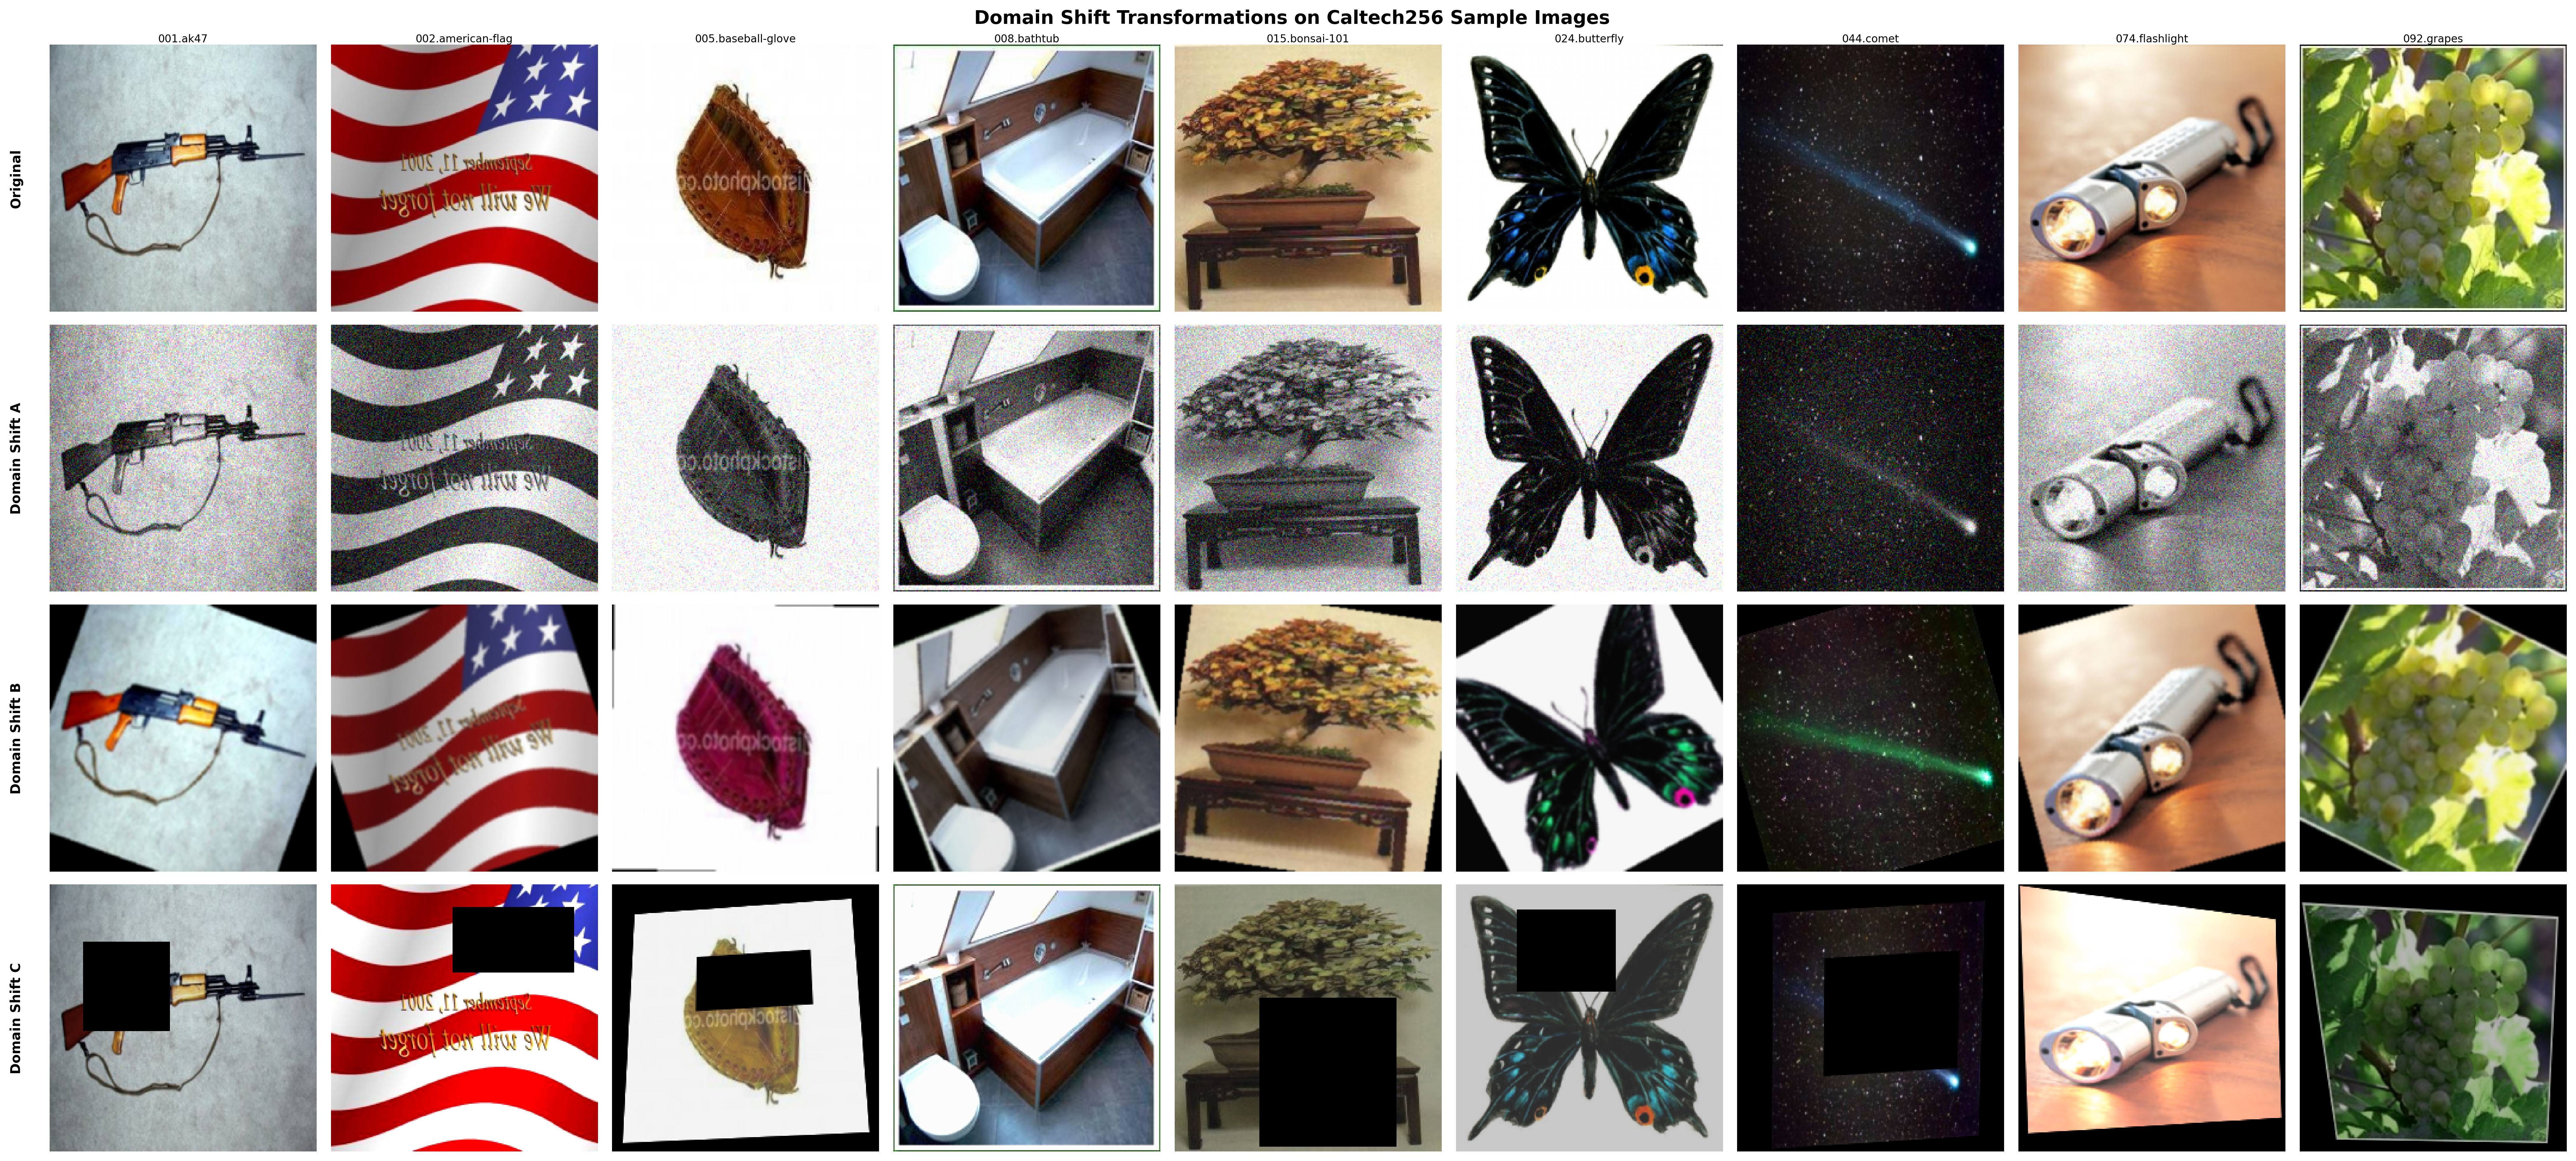
\includegraphics[width=\textwidth]{figures/domain_shift_visualization.png}

      \caption{Example images from the domain-shifted synthetic variants.
            We apply different transformations to the images of the original synthetic dataset
            to create two new domains. The first domain (Domain A) is a noisy greyscale variant,
            while the second domain (Domain B) is a rotated, blurry version of the original images,
            and the third domain (Domain C) has random erasings, shifted perspectives, and color jitter.}
      \label{fig:domain_shift}
\end{figure}

To mitigate this issue, we try to synthetically create a different domain for each variant by applying transforms to the
underlying dataset images.
An example subset of the domain-shifted images is shown in Figure~\ref{fig:domain_shift}:
Using different transforms, the images appear in unique styles and distortions,
synthetically changing their visual characteristics
while retaining the same classes and relationships.

\begin{table}[ht]
\centering
\caption{Evaluation results on test sets for domain-shifted experiments. Models were trained with different domain shift transformations and checkpointed after every epoch. The model with the lowest validation loss was selected for evaluation on the test set. Training time indicates the total duration from start to finish of model training.}
\label{tab:evaluation_results_domain_shifted}
\begin{tabular}{cccc}
\toprule
Dataset Variant & Domain & Training Time & Accuracy \\
\midrule
Caltech-256 2-Domain Domain Shifted Variant 1 & A & 1h 44m & 0.72 \\
Caltech-256 2-Domain Domain Shifted Variant 1 & B & 2h 15m & 0.76 \\
Caltech-256 2-Domain Domain Shifted Variant 2 & A & 1h 51m & 0.70 \\
Caltech-256 2-Domain Domain Shifted Variant 2 & B & 2h 27m & 0.75 \\
Caltech-256 3-Domain Domain Shifted Variant & A & 1h 42m & 0.70 \\
Caltech-256 3-Domain Domain Shifted Variant & B & 2h 20m & 0.75 \\
Caltech-256 3-Domain Domain Shifted Variant & C & 2h 22m & 0.74 \\
CIFAR-100 2-Domain Domain Shifted Variant & A & 1h 1m & 0.57 \\
CIFAR-100 2-Domain Domain Shifted Variant & B & 1h 39m & 0.63 \\
\bottomrule
\end{tabular}
\end{table}

\begin{table}[ht]
\centering
\caption{Average performance metrics for relationship discovery methods with globally optimal parameters on domain-shifted experiments. Each method uses the parameter value that minimizes the average EDR across all domain-shifted dataset variants. Performance metrics are then averaged across all dataset variants using these optimal parameters.}
\label{tab:relationship_methods_global_optimal_domain_shifted}
\begin{tabular}{lccccc}
\toprule
Method & Parameter & EDR & Precision & Recall & F1-score \\
\midrule
MCFP & N/A & 0.842 & \textbf{0.490} & 0.226 & 0.305 \\
Naive Thresholding & 0.10 & 0.761 & 0.418 & 0.519 & \textbf{0.450} \\
Density Thresholding & 0.60 & 0.766 & 0.349 & \textbf{0.582} & 0.426 \\
Relationship Hypothesis & 5 & \textbf{0.759} & 0.390 & 0.543 & 0.444 \\
\bottomrule
\end{tabular}
\end{table}


The training performance of these new domain-shifted models can be seen in Table~\ref{tab:evaluation_results_domain_shifted}.
We can observe a $10\%$ decrease in accuracy on the test data compared to the original synthetic dataset variants.
This was to be expected due to the increased complexity of the domain-shifted tasks.

When comparing the new averaged relationship method evaluation results in Table~\ref{tab:relationship_methods_global_optimal_domain_shifted}
to our original non-domain-shifted results in Table~\ref{tab:relationship_methods_global_optimal},
we can observe significant differences:

\begin{itemize}
      \item Our new best performing relationship selection method,
            based on averaged maximum EDR scores, changes from MCFP to the relationship hypothesis method.
      \item In general, all methods have a lower EDR score than their non-domain-shifted counterparts.
            This is a direct result of the decreased domain model accuracy and was to be expected.
      \item The MCFP method still has the highest relative precision with $0.49$.
            If precision is more important than EDR for a high universal model accuracy
            will be evaluated in the universal model training section (see Section~\ref{sec:universal_models}).
\end{itemize}

We will use the most promising relationship selection methods,
MCFP and relationship hypothesis, for our universal model training.
Our final evaluation will focus on the model accuracy of the trained universal Models
built with the universal taxonomies of the two preselected relationship selection methods
(using the selection method parameters that have the best EDR score).

\subsection{Universal Taxonomy Generation}

\begin{figure}[ht]
      \centering
      \includegraphics[width=0.35\textwidth]{figures/taxonomy.png}

      \caption{This figure shows the complete Caltech101-Caltech256 universal taxonomy.
            While most classes build smaller clusters build smaller clusters of 2-3 classes,
            some large clusters can be observed.}
      \label{fig:taxonomy}
\end{figure}

\begin{figure}[ht]
      \centering
      \includegraphics[width=0.35\textwidth]{figures/wheel_concept.png}

      \caption{In the Caltech101-Caltech256 universal taxonomy,
            this cluster only contains vehicles. The universal classes created can be interpreted as
            sharing a common concept of \enquote{wheel}.}
      \label{fig:wheel_concept}
\end{figure}

\begin{figure}[ht]
      \centering
      \includegraphics[width=0.35\textwidth]{figures/bad_taxonomy.png}

      \caption{This example in the Caltech101-Caltech256 universal taxonomy shows a wrong relationship
            cluster towards the Caltech101 class \enquote{binocular}. Many of the Caltech256 classes
            do not have a suitable representation in the Caltech101 dataset
            and then connect to the Caltech101 class \enquote{binocular} instead.}
      \label{fig:bad_taxonomy}
\end{figure}

We now have our domain models trained and our relationship selection methods evaluated.
In the next step, we run our universal taxonomy generation algorithm
(see Section~\ref{sec:universal_taxonomy_algorithm}) on the Caltech-101 and
Caltech-256 datasets. To make the results more interpretable,
we will use the most common foreign prediction method to have a sparse relationship graph
that is easier to look at
(for our later universal model training, we will of course work with both the naive thresholding method and the most common foreign prediction method).

The overall universal taxonomy generated from the Caltech-101 and Caltech-256 datasets
is shown in Figure~\ref{fig:taxonomy}.
We can observe many smaller clusters of 2-3 classes which build from a single domain class in
the Caltech-101 dataset and multiple domain classes in the Caltech-256 dataset
(since the Caltech-256 dataset has more granular classes, this is to be expected).

An example of a \enquote{good} cluster is shown in Figure~\ref{fig:wheel_concept}:
This cluster centers around the Caltech101 class \enquote{wheelchair} and contains
multiple Caltech256 classes that share the concept of \enquote{wheel} (e.g. \enquote{mountain bike}, \enquote{segway}, \enquote{touring bike}, etc.).
The universal classes between the Caltech101 and Caltech256 classes
will provide a useful mapping for our universal model training.

However, we can also observe \enquote{bad} clusters in the universal taxonomy,
such as the one shown in Figure~\ref{fig:bad_taxonomy}:
The Caltech101 class \enquote{binocular} is connected to multiple Caltech256 classes
of a variety of different concepts.
While many of these classes do share concepts with binoculars (e.g. \enquote{sextant}, \enquote{telescope}, etc.),
many of the Caltech256 classes in the cluster do not have an obvious connection to binoculars
(e.g. \enquote{boxing glove}, \enquote{fire extinguisher}, etc.).
Since it is likely that the Caltech256 dataset contains classes that do not have a suitable representation in the Caltech101 dataset,
we \enquote{force} a relationship to a Caltech101 class by using the most common foreign prediction method.
However, the incorrect relationships do have a low relationship weight which makes
the error less severe for the universal model training.

Addressing these issues is a complex task, since a suitable threshold for the relationship weights
depends on the individual composition of the datasets.


\section{Universal Models} \label{sec:universal_models}

\subsection{Training}

\subsubsection{Modifications to Baseline Architecture}

Building upon the ResNet-50 architecture used for the individual domain models, we developed a \texttt{UniversalResNetModel} that incorporates several key modifications to enable multi-domain training through our universal taxonomy approach.

The most significant architectural change is the replacement of the standard classification head. While the baseline \texttt{ResNetModel} uses a multi-layer fully connected classifier with dropout regularization that outputs logits for domain-specific classes, the \texttt{UniversalResNetModel} employs a simplified two-layer fully connected head that outputs logits for universal classes:

\begin{itemize}
      \item \textbf{Baseline classifier}: A 6-layer fully connected network with dropout (0.5, 0.2, 0.2, 0.2, 0.2) that progressively reduces dimensionality from ResNet features $\rightarrow$ 1024 $\rightarrow$ 512 $\rightarrow$ 256 $\rightarrow$ 128 $\rightarrow$ domain classes
      \item \textbf{Universal classifier}: A 2-layer fully connected network (ResNet features $\rightarrow$ 1024 $\rightarrow$ universal classes) without dropout regularization
\end{itemize}

The simplified architecture proved to be more effective in training runs vs. the more complex hopper + dropout architecture used in the baseline models.

Another crucial modification is the loss function:
The baseline models use standard cross-entropy loss with one-hot encoded targets,
while the universal model employs cross-entropy for discrete probability distributions for a loss function.
This change accommodates the fact that domain classes may map to multiple universal classes with different weights,
as determined by the taxonomy relationships
(full explanation in Section~\ref{sec:universal_model_learning}).

\subsubsection{Multi-Domain Training Procedure}

Instead of training separate models on individual datasets,
we create a new combined dataset that merges multiple datasets while preserving domain identity.
Each training sample is augmented with a domain identifier,
transforming the standard $(\texttt{image}, \texttt{label})$ pairs into $(\texttt{image}, (\texttt{domain\_id}, \texttt{label}))$ tuples.
This allows the model to handle samples from different datasets within the same batch
(since we need to know the image domain to apply the correct target mapping).

\begin{table}[ht]
\centering
\caption{Universal model evaluation results on multi-domain test datasets. Two-domain models were trained on Caltech-101 + Caltech-256, while the three-domain model was trained on all three datasets. Models were evaluated on individual domains as well as the combined test set. Domain accuracy values show performance compared to single-domain ResNet-50 baselines (Caltech-101: 97.23\%, Caltech-256: 75.65\%, CIFAR-100: 78.26\%). All accuracy values are shown as percentages.}
\label{tab:universal_model_results}
\begin{tabular}{lcccccc}
\toprule
Taxonomy & Training Time & Caltech-101 & Caltech-256 & CIFAR-100 & Avg \\
\midrule
Hypothesis (2) & 2h 7m & 91.93 (-5.30) & 82.45 (+6.80) & N/A & 84.670000 \\
MCFP (2) & 2h 17m & 91.70 (-5.53) & 80.10 (+4.45) & N/A & 82.760000 \\
Hypothesis (3) & 4h 58m & 96.19 (-1.04) & 86.80 (+11.15) & 75.20 (+15.92) & 78.990000 \\
MCFP (3) & 4h 59m & 83.51 (-13.72) & 77.55 (+1.90) & 76.10 (+16.82) & 76.630000 \\
\bottomrule
\end{tabular}
\end{table}


\begin{figure}[ht]
      \centering
      \scalebox{0.35}{%% Creator: Matplotlib, PGF backend
%%
%% To include the figure in your LaTeX document, write
%%   \input{<filename>.pgf}
%%
%% Make sure the required packages are loaded in your preamble
%%   \usepackage{pgf}
%%
%% Also ensure that all the required font packages are loaded; for instance,
%% the lmodern package is sometimes necessary when using math font.
%%   \usepackage{lmodern}
%%
%% Figures using additional raster images can only be included by \input if
%% they are in the same directory as the main LaTeX file. For loading figures
%% from other directories you can use the `import` package
%%   \usepackage{import}
%%
%% and then include the figures with
%%   \import{<path to file>}{<filename>.pgf}
%%
%% Matplotlib used the following preamble
%%   \def\mathdefault#1{#1}
%%   \everymath=\expandafter{\the\everymath\displaystyle}
%%   \IfFileExists{scrextend.sty}{
%%     \usepackage[fontsize=11.000000pt]{scrextend}
%%   }{
%%     \renewcommand{\normalsize}{\fontsize{11.000000}{13.200000}\selectfont}
%%     \normalsize
%%   }
%%   
%%   \ifdefined\pdftexversion\else  % non-pdftex case.
%%     \usepackage{fontspec}
%%     \setmainfont{DejaVuSerif.ttf}[Path=\detokenize{/home/bjoern/miniconda3/envs/master-thesis/lib/python3.13/site-packages/matplotlib/mpl-data/fonts/ttf/}]
%%     \setsansfont{DejaVuSans.ttf}[Path=\detokenize{/home/bjoern/miniconda3/envs/master-thesis/lib/python3.13/site-packages/matplotlib/mpl-data/fonts/ttf/}]
%%     \setmonofont{DejaVuSansMono.ttf}[Path=\detokenize{/home/bjoern/miniconda3/envs/master-thesis/lib/python3.13/site-packages/matplotlib/mpl-data/fonts/ttf/}]
%%   \fi
%%   \makeatletter\@ifpackageloaded{underscore}{}{\usepackage[strings]{underscore}}\makeatother
%%
\begingroup%
\makeatletter%
\begin{pgfpicture}%
\pgfpathrectangle{\pgfpointorigin}{\pgfqpoint{24.843212in}{9.870000in}}%
\pgfusepath{use as bounding box, clip}%
\begin{pgfscope}%
\pgfsetbuttcap%
\pgfsetmiterjoin%
\definecolor{currentfill}{rgb}{1.000000,1.000000,1.000000}%
\pgfsetfillcolor{currentfill}%
\pgfsetlinewidth{0.000000pt}%
\definecolor{currentstroke}{rgb}{1.000000,1.000000,1.000000}%
\pgfsetstrokecolor{currentstroke}%
\pgfsetdash{}{0pt}%
\pgfpathmoveto{\pgfqpoint{0.000000in}{0.000000in}}%
\pgfpathlineto{\pgfqpoint{24.843212in}{0.000000in}}%
\pgfpathlineto{\pgfqpoint{24.843212in}{9.870000in}}%
\pgfpathlineto{\pgfqpoint{0.000000in}{9.870000in}}%
\pgfpathlineto{\pgfqpoint{0.000000in}{0.000000in}}%
\pgfpathclose%
\pgfusepath{fill}%
\end{pgfscope}%
\begin{pgfscope}%
\pgfsetbuttcap%
\pgfsetmiterjoin%
\definecolor{currentfill}{rgb}{1.000000,1.000000,1.000000}%
\pgfsetfillcolor{currentfill}%
\pgfsetlinewidth{0.000000pt}%
\definecolor{currentstroke}{rgb}{0.000000,0.000000,0.000000}%
\pgfsetstrokecolor{currentstroke}%
\pgfsetstrokeopacity{0.000000}%
\pgfsetdash{}{0pt}%
\pgfpathmoveto{\pgfqpoint{0.598357in}{5.472778in}}%
\pgfpathlineto{\pgfqpoint{4.814134in}{5.472778in}}%
\pgfpathlineto{\pgfqpoint{4.814134in}{9.598542in}}%
\pgfpathlineto{\pgfqpoint{0.598357in}{9.598542in}}%
\pgfpathlineto{\pgfqpoint{0.598357in}{5.472778in}}%
\pgfpathclose%
\pgfusepath{fill}%
\end{pgfscope}%
\begin{pgfscope}%
\pgfpathrectangle{\pgfqpoint{0.598357in}{5.472778in}}{\pgfqpoint{4.215777in}{4.125764in}}%
\pgfusepath{clip}%
\pgfsetrectcap%
\pgfsetroundjoin%
\pgfsetlinewidth{0.803000pt}%
\definecolor{currentstroke}{rgb}{0.690196,0.690196,0.690196}%
\pgfsetstrokecolor{currentstroke}%
\pgfsetstrokeopacity{0.300000}%
\pgfsetdash{}{0pt}%
\pgfpathmoveto{\pgfqpoint{0.782333in}{5.472778in}}%
\pgfpathlineto{\pgfqpoint{0.782333in}{9.598542in}}%
\pgfusepath{stroke}%
\end{pgfscope}%
\begin{pgfscope}%
\pgfsetbuttcap%
\pgfsetroundjoin%
\definecolor{currentfill}{rgb}{0.000000,0.000000,0.000000}%
\pgfsetfillcolor{currentfill}%
\pgfsetlinewidth{0.803000pt}%
\definecolor{currentstroke}{rgb}{0.000000,0.000000,0.000000}%
\pgfsetstrokecolor{currentstroke}%
\pgfsetdash{}{0pt}%
\pgfsys@defobject{currentmarker}{\pgfqpoint{0.000000in}{-0.048611in}}{\pgfqpoint{0.000000in}{0.000000in}}{%
\pgfpathmoveto{\pgfqpoint{0.000000in}{0.000000in}}%
\pgfpathlineto{\pgfqpoint{0.000000in}{-0.048611in}}%
\pgfusepath{stroke,fill}%
}%
\begin{pgfscope}%
\pgfsys@transformshift{0.782333in}{5.472778in}%
\pgfsys@useobject{currentmarker}{}%
\end{pgfscope}%
\end{pgfscope}%
\begin{pgfscope}%
\definecolor{textcolor}{rgb}{0.000000,0.000000,0.000000}%
\pgfsetstrokecolor{textcolor}%
\pgfsetfillcolor{textcolor}%
\pgftext[x=0.782333in,y=5.375556in,,top]{\color{textcolor}{\ifdefined\pdftexversion\else\setmainfont{EB Garamond}\rmfamily\fi\fontsize{11.000000}{13.200000}\selectfont\catcode`\^=\active\def^{\ifmmode\sp\else\^{}\fi}\catcode`\%=\active\def%{\%}$\mathdefault{0}$}}%
\end{pgfscope}%
\begin{pgfscope}%
\pgfpathrectangle{\pgfqpoint{0.598357in}{5.472778in}}{\pgfqpoint{4.215777in}{4.125764in}}%
\pgfusepath{clip}%
\pgfsetrectcap%
\pgfsetroundjoin%
\pgfsetlinewidth{0.803000pt}%
\definecolor{currentstroke}{rgb}{0.690196,0.690196,0.690196}%
\pgfsetstrokecolor{currentstroke}%
\pgfsetstrokeopacity{0.300000}%
\pgfsetdash{}{0pt}%
\pgfpathmoveto{\pgfqpoint{1.562888in}{5.472778in}}%
\pgfpathlineto{\pgfqpoint{1.562888in}{9.598542in}}%
\pgfusepath{stroke}%
\end{pgfscope}%
\begin{pgfscope}%
\pgfsetbuttcap%
\pgfsetroundjoin%
\definecolor{currentfill}{rgb}{0.000000,0.000000,0.000000}%
\pgfsetfillcolor{currentfill}%
\pgfsetlinewidth{0.803000pt}%
\definecolor{currentstroke}{rgb}{0.000000,0.000000,0.000000}%
\pgfsetstrokecolor{currentstroke}%
\pgfsetdash{}{0pt}%
\pgfsys@defobject{currentmarker}{\pgfqpoint{0.000000in}{-0.048611in}}{\pgfqpoint{0.000000in}{0.000000in}}{%
\pgfpathmoveto{\pgfqpoint{0.000000in}{0.000000in}}%
\pgfpathlineto{\pgfqpoint{0.000000in}{-0.048611in}}%
\pgfusepath{stroke,fill}%
}%
\begin{pgfscope}%
\pgfsys@transformshift{1.562888in}{5.472778in}%
\pgfsys@useobject{currentmarker}{}%
\end{pgfscope}%
\end{pgfscope}%
\begin{pgfscope}%
\definecolor{textcolor}{rgb}{0.000000,0.000000,0.000000}%
\pgfsetstrokecolor{textcolor}%
\pgfsetfillcolor{textcolor}%
\pgftext[x=1.562888in,y=5.375556in,,top]{\color{textcolor}{\ifdefined\pdftexversion\else\setmainfont{EB Garamond}\rmfamily\fi\fontsize{11.000000}{13.200000}\selectfont\catcode`\^=\active\def^{\ifmmode\sp\else\^{}\fi}\catcode`\%=\active\def%{\%}$\mathdefault{5000}$}}%
\end{pgfscope}%
\begin{pgfscope}%
\pgfpathrectangle{\pgfqpoint{0.598357in}{5.472778in}}{\pgfqpoint{4.215777in}{4.125764in}}%
\pgfusepath{clip}%
\pgfsetrectcap%
\pgfsetroundjoin%
\pgfsetlinewidth{0.803000pt}%
\definecolor{currentstroke}{rgb}{0.690196,0.690196,0.690196}%
\pgfsetstrokecolor{currentstroke}%
\pgfsetstrokeopacity{0.300000}%
\pgfsetdash{}{0pt}%
\pgfpathmoveto{\pgfqpoint{2.343443in}{5.472778in}}%
\pgfpathlineto{\pgfqpoint{2.343443in}{9.598542in}}%
\pgfusepath{stroke}%
\end{pgfscope}%
\begin{pgfscope}%
\pgfsetbuttcap%
\pgfsetroundjoin%
\definecolor{currentfill}{rgb}{0.000000,0.000000,0.000000}%
\pgfsetfillcolor{currentfill}%
\pgfsetlinewidth{0.803000pt}%
\definecolor{currentstroke}{rgb}{0.000000,0.000000,0.000000}%
\pgfsetstrokecolor{currentstroke}%
\pgfsetdash{}{0pt}%
\pgfsys@defobject{currentmarker}{\pgfqpoint{0.000000in}{-0.048611in}}{\pgfqpoint{0.000000in}{0.000000in}}{%
\pgfpathmoveto{\pgfqpoint{0.000000in}{0.000000in}}%
\pgfpathlineto{\pgfqpoint{0.000000in}{-0.048611in}}%
\pgfusepath{stroke,fill}%
}%
\begin{pgfscope}%
\pgfsys@transformshift{2.343443in}{5.472778in}%
\pgfsys@useobject{currentmarker}{}%
\end{pgfscope}%
\end{pgfscope}%
\begin{pgfscope}%
\definecolor{textcolor}{rgb}{0.000000,0.000000,0.000000}%
\pgfsetstrokecolor{textcolor}%
\pgfsetfillcolor{textcolor}%
\pgftext[x=2.343443in,y=5.375556in,,top]{\color{textcolor}{\ifdefined\pdftexversion\else\setmainfont{EB Garamond}\rmfamily\fi\fontsize{11.000000}{13.200000}\selectfont\catcode`\^=\active\def^{\ifmmode\sp\else\^{}\fi}\catcode`\%=\active\def%{\%}$\mathdefault{10000}$}}%
\end{pgfscope}%
\begin{pgfscope}%
\pgfpathrectangle{\pgfqpoint{0.598357in}{5.472778in}}{\pgfqpoint{4.215777in}{4.125764in}}%
\pgfusepath{clip}%
\pgfsetrectcap%
\pgfsetroundjoin%
\pgfsetlinewidth{0.803000pt}%
\definecolor{currentstroke}{rgb}{0.690196,0.690196,0.690196}%
\pgfsetstrokecolor{currentstroke}%
\pgfsetstrokeopacity{0.300000}%
\pgfsetdash{}{0pt}%
\pgfpathmoveto{\pgfqpoint{3.123998in}{5.472778in}}%
\pgfpathlineto{\pgfqpoint{3.123998in}{9.598542in}}%
\pgfusepath{stroke}%
\end{pgfscope}%
\begin{pgfscope}%
\pgfsetbuttcap%
\pgfsetroundjoin%
\definecolor{currentfill}{rgb}{0.000000,0.000000,0.000000}%
\pgfsetfillcolor{currentfill}%
\pgfsetlinewidth{0.803000pt}%
\definecolor{currentstroke}{rgb}{0.000000,0.000000,0.000000}%
\pgfsetstrokecolor{currentstroke}%
\pgfsetdash{}{0pt}%
\pgfsys@defobject{currentmarker}{\pgfqpoint{0.000000in}{-0.048611in}}{\pgfqpoint{0.000000in}{0.000000in}}{%
\pgfpathmoveto{\pgfqpoint{0.000000in}{0.000000in}}%
\pgfpathlineto{\pgfqpoint{0.000000in}{-0.048611in}}%
\pgfusepath{stroke,fill}%
}%
\begin{pgfscope}%
\pgfsys@transformshift{3.123998in}{5.472778in}%
\pgfsys@useobject{currentmarker}{}%
\end{pgfscope}%
\end{pgfscope}%
\begin{pgfscope}%
\definecolor{textcolor}{rgb}{0.000000,0.000000,0.000000}%
\pgfsetstrokecolor{textcolor}%
\pgfsetfillcolor{textcolor}%
\pgftext[x=3.123998in,y=5.375556in,,top]{\color{textcolor}{\ifdefined\pdftexversion\else\setmainfont{EB Garamond}\rmfamily\fi\fontsize{11.000000}{13.200000}\selectfont\catcode`\^=\active\def^{\ifmmode\sp\else\^{}\fi}\catcode`\%=\active\def%{\%}$\mathdefault{15000}$}}%
\end{pgfscope}%
\begin{pgfscope}%
\pgfpathrectangle{\pgfqpoint{0.598357in}{5.472778in}}{\pgfqpoint{4.215777in}{4.125764in}}%
\pgfusepath{clip}%
\pgfsetrectcap%
\pgfsetroundjoin%
\pgfsetlinewidth{0.803000pt}%
\definecolor{currentstroke}{rgb}{0.690196,0.690196,0.690196}%
\pgfsetstrokecolor{currentstroke}%
\pgfsetstrokeopacity{0.300000}%
\pgfsetdash{}{0pt}%
\pgfpathmoveto{\pgfqpoint{3.904553in}{5.472778in}}%
\pgfpathlineto{\pgfqpoint{3.904553in}{9.598542in}}%
\pgfusepath{stroke}%
\end{pgfscope}%
\begin{pgfscope}%
\pgfsetbuttcap%
\pgfsetroundjoin%
\definecolor{currentfill}{rgb}{0.000000,0.000000,0.000000}%
\pgfsetfillcolor{currentfill}%
\pgfsetlinewidth{0.803000pt}%
\definecolor{currentstroke}{rgb}{0.000000,0.000000,0.000000}%
\pgfsetstrokecolor{currentstroke}%
\pgfsetdash{}{0pt}%
\pgfsys@defobject{currentmarker}{\pgfqpoint{0.000000in}{-0.048611in}}{\pgfqpoint{0.000000in}{0.000000in}}{%
\pgfpathmoveto{\pgfqpoint{0.000000in}{0.000000in}}%
\pgfpathlineto{\pgfqpoint{0.000000in}{-0.048611in}}%
\pgfusepath{stroke,fill}%
}%
\begin{pgfscope}%
\pgfsys@transformshift{3.904553in}{5.472778in}%
\pgfsys@useobject{currentmarker}{}%
\end{pgfscope}%
\end{pgfscope}%
\begin{pgfscope}%
\definecolor{textcolor}{rgb}{0.000000,0.000000,0.000000}%
\pgfsetstrokecolor{textcolor}%
\pgfsetfillcolor{textcolor}%
\pgftext[x=3.904553in,y=5.375556in,,top]{\color{textcolor}{\ifdefined\pdftexversion\else\setmainfont{EB Garamond}\rmfamily\fi\fontsize{11.000000}{13.200000}\selectfont\catcode`\^=\active\def^{\ifmmode\sp\else\^{}\fi}\catcode`\%=\active\def%{\%}$\mathdefault{20000}$}}%
\end{pgfscope}%
\begin{pgfscope}%
\pgfpathrectangle{\pgfqpoint{0.598357in}{5.472778in}}{\pgfqpoint{4.215777in}{4.125764in}}%
\pgfusepath{clip}%
\pgfsetrectcap%
\pgfsetroundjoin%
\pgfsetlinewidth{0.803000pt}%
\definecolor{currentstroke}{rgb}{0.690196,0.690196,0.690196}%
\pgfsetstrokecolor{currentstroke}%
\pgfsetstrokeopacity{0.300000}%
\pgfsetdash{}{0pt}%
\pgfpathmoveto{\pgfqpoint{4.685108in}{5.472778in}}%
\pgfpathlineto{\pgfqpoint{4.685108in}{9.598542in}}%
\pgfusepath{stroke}%
\end{pgfscope}%
\begin{pgfscope}%
\pgfsetbuttcap%
\pgfsetroundjoin%
\definecolor{currentfill}{rgb}{0.000000,0.000000,0.000000}%
\pgfsetfillcolor{currentfill}%
\pgfsetlinewidth{0.803000pt}%
\definecolor{currentstroke}{rgb}{0.000000,0.000000,0.000000}%
\pgfsetstrokecolor{currentstroke}%
\pgfsetdash{}{0pt}%
\pgfsys@defobject{currentmarker}{\pgfqpoint{0.000000in}{-0.048611in}}{\pgfqpoint{0.000000in}{0.000000in}}{%
\pgfpathmoveto{\pgfqpoint{0.000000in}{0.000000in}}%
\pgfpathlineto{\pgfqpoint{0.000000in}{-0.048611in}}%
\pgfusepath{stroke,fill}%
}%
\begin{pgfscope}%
\pgfsys@transformshift{4.685108in}{5.472778in}%
\pgfsys@useobject{currentmarker}{}%
\end{pgfscope}%
\end{pgfscope}%
\begin{pgfscope}%
\definecolor{textcolor}{rgb}{0.000000,0.000000,0.000000}%
\pgfsetstrokecolor{textcolor}%
\pgfsetfillcolor{textcolor}%
\pgftext[x=4.685108in,y=5.375556in,,top]{\color{textcolor}{\ifdefined\pdftexversion\else\setmainfont{EB Garamond}\rmfamily\fi\fontsize{11.000000}{13.200000}\selectfont\catcode`\^=\active\def^{\ifmmode\sp\else\^{}\fi}\catcode`\%=\active\def%{\%}$\mathdefault{25000}$}}%
\end{pgfscope}%
\begin{pgfscope}%
\definecolor{textcolor}{rgb}{0.000000,0.000000,0.000000}%
\pgfsetstrokecolor{textcolor}%
\pgfsetfillcolor{textcolor}%
\pgftext[x=2.706245in,y=5.168750in,,top]{\color{textcolor}{\ifdefined\pdftexversion\else\setmainfont{EB Garamond}\rmfamily\fi\fontsize{11.000000}{13.200000}\selectfont\catcode`\^=\active\def^{\ifmmode\sp\else\^{}\fi}\catcode`\%=\active\def%{\%}Steps}}%
\end{pgfscope}%
\begin{pgfscope}%
\pgfpathrectangle{\pgfqpoint{0.598357in}{5.472778in}}{\pgfqpoint{4.215777in}{4.125764in}}%
\pgfusepath{clip}%
\pgfsetrectcap%
\pgfsetroundjoin%
\pgfsetlinewidth{0.803000pt}%
\definecolor{currentstroke}{rgb}{0.690196,0.690196,0.690196}%
\pgfsetstrokecolor{currentstroke}%
\pgfsetstrokeopacity{0.300000}%
\pgfsetdash{}{0pt}%
\pgfpathmoveto{\pgfqpoint{0.598357in}{6.041962in}}%
\pgfpathlineto{\pgfqpoint{4.814134in}{6.041962in}}%
\pgfusepath{stroke}%
\end{pgfscope}%
\begin{pgfscope}%
\pgfsetbuttcap%
\pgfsetroundjoin%
\definecolor{currentfill}{rgb}{0.000000,0.000000,0.000000}%
\pgfsetfillcolor{currentfill}%
\pgfsetlinewidth{0.803000pt}%
\definecolor{currentstroke}{rgb}{0.000000,0.000000,0.000000}%
\pgfsetstrokecolor{currentstroke}%
\pgfsetdash{}{0pt}%
\pgfsys@defobject{currentmarker}{\pgfqpoint{-0.048611in}{0.000000in}}{\pgfqpoint{-0.000000in}{0.000000in}}{%
\pgfpathmoveto{\pgfqpoint{-0.000000in}{0.000000in}}%
\pgfpathlineto{\pgfqpoint{-0.048611in}{0.000000in}}%
\pgfusepath{stroke,fill}%
}%
\begin{pgfscope}%
\pgfsys@transformshift{0.598357in}{6.041962in}%
\pgfsys@useobject{currentmarker}{}%
\end{pgfscope}%
\end{pgfscope}%
\begin{pgfscope}%
\definecolor{textcolor}{rgb}{0.000000,0.000000,0.000000}%
\pgfsetstrokecolor{textcolor}%
\pgfsetfillcolor{textcolor}%
\pgftext[x=0.306806in, y=5.988108in, left, base]{\color{textcolor}{\ifdefined\pdftexversion\else\setmainfont{EB Garamond}\rmfamily\fi\fontsize{11.000000}{13.200000}\selectfont\catcode`\^=\active\def^{\ifmmode\sp\else\^{}\fi}\catcode`\%=\active\def%{\%}$\mathdefault{0.2}$}}%
\end{pgfscope}%
\begin{pgfscope}%
\pgfpathrectangle{\pgfqpoint{0.598357in}{5.472778in}}{\pgfqpoint{4.215777in}{4.125764in}}%
\pgfusepath{clip}%
\pgfsetrectcap%
\pgfsetroundjoin%
\pgfsetlinewidth{0.803000pt}%
\definecolor{currentstroke}{rgb}{0.690196,0.690196,0.690196}%
\pgfsetstrokecolor{currentstroke}%
\pgfsetstrokeopacity{0.300000}%
\pgfsetdash{}{0pt}%
\pgfpathmoveto{\pgfqpoint{0.598357in}{6.884223in}}%
\pgfpathlineto{\pgfqpoint{4.814134in}{6.884223in}}%
\pgfusepath{stroke}%
\end{pgfscope}%
\begin{pgfscope}%
\pgfsetbuttcap%
\pgfsetroundjoin%
\definecolor{currentfill}{rgb}{0.000000,0.000000,0.000000}%
\pgfsetfillcolor{currentfill}%
\pgfsetlinewidth{0.803000pt}%
\definecolor{currentstroke}{rgb}{0.000000,0.000000,0.000000}%
\pgfsetstrokecolor{currentstroke}%
\pgfsetdash{}{0pt}%
\pgfsys@defobject{currentmarker}{\pgfqpoint{-0.048611in}{0.000000in}}{\pgfqpoint{-0.000000in}{0.000000in}}{%
\pgfpathmoveto{\pgfqpoint{-0.000000in}{0.000000in}}%
\pgfpathlineto{\pgfqpoint{-0.048611in}{0.000000in}}%
\pgfusepath{stroke,fill}%
}%
\begin{pgfscope}%
\pgfsys@transformshift{0.598357in}{6.884223in}%
\pgfsys@useobject{currentmarker}{}%
\end{pgfscope}%
\end{pgfscope}%
\begin{pgfscope}%
\definecolor{textcolor}{rgb}{0.000000,0.000000,0.000000}%
\pgfsetstrokecolor{textcolor}%
\pgfsetfillcolor{textcolor}%
\pgftext[x=0.306806in, y=6.830369in, left, base]{\color{textcolor}{\ifdefined\pdftexversion\else\setmainfont{EB Garamond}\rmfamily\fi\fontsize{11.000000}{13.200000}\selectfont\catcode`\^=\active\def^{\ifmmode\sp\else\^{}\fi}\catcode`\%=\active\def%{\%}$\mathdefault{0.4}$}}%
\end{pgfscope}%
\begin{pgfscope}%
\pgfpathrectangle{\pgfqpoint{0.598357in}{5.472778in}}{\pgfqpoint{4.215777in}{4.125764in}}%
\pgfusepath{clip}%
\pgfsetrectcap%
\pgfsetroundjoin%
\pgfsetlinewidth{0.803000pt}%
\definecolor{currentstroke}{rgb}{0.690196,0.690196,0.690196}%
\pgfsetstrokecolor{currentstroke}%
\pgfsetstrokeopacity{0.300000}%
\pgfsetdash{}{0pt}%
\pgfpathmoveto{\pgfqpoint{0.598357in}{7.726485in}}%
\pgfpathlineto{\pgfqpoint{4.814134in}{7.726485in}}%
\pgfusepath{stroke}%
\end{pgfscope}%
\begin{pgfscope}%
\pgfsetbuttcap%
\pgfsetroundjoin%
\definecolor{currentfill}{rgb}{0.000000,0.000000,0.000000}%
\pgfsetfillcolor{currentfill}%
\pgfsetlinewidth{0.803000pt}%
\definecolor{currentstroke}{rgb}{0.000000,0.000000,0.000000}%
\pgfsetstrokecolor{currentstroke}%
\pgfsetdash{}{0pt}%
\pgfsys@defobject{currentmarker}{\pgfqpoint{-0.048611in}{0.000000in}}{\pgfqpoint{-0.000000in}{0.000000in}}{%
\pgfpathmoveto{\pgfqpoint{-0.000000in}{0.000000in}}%
\pgfpathlineto{\pgfqpoint{-0.048611in}{0.000000in}}%
\pgfusepath{stroke,fill}%
}%
\begin{pgfscope}%
\pgfsys@transformshift{0.598357in}{7.726485in}%
\pgfsys@useobject{currentmarker}{}%
\end{pgfscope}%
\end{pgfscope}%
\begin{pgfscope}%
\definecolor{textcolor}{rgb}{0.000000,0.000000,0.000000}%
\pgfsetstrokecolor{textcolor}%
\pgfsetfillcolor{textcolor}%
\pgftext[x=0.306806in, y=7.672630in, left, base]{\color{textcolor}{\ifdefined\pdftexversion\else\setmainfont{EB Garamond}\rmfamily\fi\fontsize{11.000000}{13.200000}\selectfont\catcode`\^=\active\def^{\ifmmode\sp\else\^{}\fi}\catcode`\%=\active\def%{\%}$\mathdefault{0.6}$}}%
\end{pgfscope}%
\begin{pgfscope}%
\pgfpathrectangle{\pgfqpoint{0.598357in}{5.472778in}}{\pgfqpoint{4.215777in}{4.125764in}}%
\pgfusepath{clip}%
\pgfsetrectcap%
\pgfsetroundjoin%
\pgfsetlinewidth{0.803000pt}%
\definecolor{currentstroke}{rgb}{0.690196,0.690196,0.690196}%
\pgfsetstrokecolor{currentstroke}%
\pgfsetstrokeopacity{0.300000}%
\pgfsetdash{}{0pt}%
\pgfpathmoveto{\pgfqpoint{0.598357in}{8.568746in}}%
\pgfpathlineto{\pgfqpoint{4.814134in}{8.568746in}}%
\pgfusepath{stroke}%
\end{pgfscope}%
\begin{pgfscope}%
\pgfsetbuttcap%
\pgfsetroundjoin%
\definecolor{currentfill}{rgb}{0.000000,0.000000,0.000000}%
\pgfsetfillcolor{currentfill}%
\pgfsetlinewidth{0.803000pt}%
\definecolor{currentstroke}{rgb}{0.000000,0.000000,0.000000}%
\pgfsetstrokecolor{currentstroke}%
\pgfsetdash{}{0pt}%
\pgfsys@defobject{currentmarker}{\pgfqpoint{-0.048611in}{0.000000in}}{\pgfqpoint{-0.000000in}{0.000000in}}{%
\pgfpathmoveto{\pgfqpoint{-0.000000in}{0.000000in}}%
\pgfpathlineto{\pgfqpoint{-0.048611in}{0.000000in}}%
\pgfusepath{stroke,fill}%
}%
\begin{pgfscope}%
\pgfsys@transformshift{0.598357in}{8.568746in}%
\pgfsys@useobject{currentmarker}{}%
\end{pgfscope}%
\end{pgfscope}%
\begin{pgfscope}%
\definecolor{textcolor}{rgb}{0.000000,0.000000,0.000000}%
\pgfsetstrokecolor{textcolor}%
\pgfsetfillcolor{textcolor}%
\pgftext[x=0.306806in, y=8.514892in, left, base]{\color{textcolor}{\ifdefined\pdftexversion\else\setmainfont{EB Garamond}\rmfamily\fi\fontsize{11.000000}{13.200000}\selectfont\catcode`\^=\active\def^{\ifmmode\sp\else\^{}\fi}\catcode`\%=\active\def%{\%}$\mathdefault{0.8}$}}%
\end{pgfscope}%
\begin{pgfscope}%
\pgfpathrectangle{\pgfqpoint{0.598357in}{5.472778in}}{\pgfqpoint{4.215777in}{4.125764in}}%
\pgfusepath{clip}%
\pgfsetrectcap%
\pgfsetroundjoin%
\pgfsetlinewidth{0.803000pt}%
\definecolor{currentstroke}{rgb}{0.690196,0.690196,0.690196}%
\pgfsetstrokecolor{currentstroke}%
\pgfsetstrokeopacity{0.300000}%
\pgfsetdash{}{0pt}%
\pgfpathmoveto{\pgfqpoint{0.598357in}{9.411007in}}%
\pgfpathlineto{\pgfqpoint{4.814134in}{9.411007in}}%
\pgfusepath{stroke}%
\end{pgfscope}%
\begin{pgfscope}%
\pgfsetbuttcap%
\pgfsetroundjoin%
\definecolor{currentfill}{rgb}{0.000000,0.000000,0.000000}%
\pgfsetfillcolor{currentfill}%
\pgfsetlinewidth{0.803000pt}%
\definecolor{currentstroke}{rgb}{0.000000,0.000000,0.000000}%
\pgfsetstrokecolor{currentstroke}%
\pgfsetdash{}{0pt}%
\pgfsys@defobject{currentmarker}{\pgfqpoint{-0.048611in}{0.000000in}}{\pgfqpoint{-0.000000in}{0.000000in}}{%
\pgfpathmoveto{\pgfqpoint{-0.000000in}{0.000000in}}%
\pgfpathlineto{\pgfqpoint{-0.048611in}{0.000000in}}%
\pgfusepath{stroke,fill}%
}%
\begin{pgfscope}%
\pgfsys@transformshift{0.598357in}{9.411007in}%
\pgfsys@useobject{currentmarker}{}%
\end{pgfscope}%
\end{pgfscope}%
\begin{pgfscope}%
\definecolor{textcolor}{rgb}{0.000000,0.000000,0.000000}%
\pgfsetstrokecolor{textcolor}%
\pgfsetfillcolor{textcolor}%
\pgftext[x=0.306806in, y=9.357153in, left, base]{\color{textcolor}{\ifdefined\pdftexversion\else\setmainfont{EB Garamond}\rmfamily\fi\fontsize{11.000000}{13.200000}\selectfont\catcode`\^=\active\def^{\ifmmode\sp\else\^{}\fi}\catcode`\%=\active\def%{\%}$\mathdefault{1.0}$}}%
\end{pgfscope}%
\begin{pgfscope}%
\definecolor{textcolor}{rgb}{0.000000,0.000000,0.000000}%
\pgfsetstrokecolor{textcolor}%
\pgfsetfillcolor{textcolor}%
\pgftext[x=0.251250in,y=7.535660in,,bottom,rotate=90.000000]{\color{textcolor}{\ifdefined\pdftexversion\else\setmainfont{EB Garamond}\rmfamily\fi\fontsize{11.000000}{13.200000}\selectfont\catcode`\^=\active\def^{\ifmmode\sp\else\^{}\fi}\catcode`\%=\active\def%{\%}Accuracy}}%
\end{pgfscope}%
\begin{pgfscope}%
\pgfpathrectangle{\pgfqpoint{0.598357in}{5.472778in}}{\pgfqpoint{4.215777in}{4.125764in}}%
\pgfusepath{clip}%
\pgfsetrectcap%
\pgfsetroundjoin%
\pgfsetlinewidth{1.505625pt}%
\definecolor{currentstroke}{rgb}{0.000000,0.000000,1.000000}%
\pgfsetstrokecolor{currentstroke}%
\pgfsetdash{}{0pt}%
\pgfpathmoveto{\pgfqpoint{0.789983in}{5.660312in}}%
\pgfpathlineto{\pgfqpoint{0.797788in}{6.384131in}}%
\pgfpathlineto{\pgfqpoint{0.813400in}{6.384131in}}%
\pgfpathlineto{\pgfqpoint{0.821205in}{6.515734in}}%
\pgfpathlineto{\pgfqpoint{0.829011in}{6.910544in}}%
\pgfpathlineto{\pgfqpoint{0.836816in}{6.647337in}}%
\pgfpathlineto{\pgfqpoint{0.844622in}{7.305354in}}%
\pgfpathlineto{\pgfqpoint{0.852427in}{7.239552in}}%
\pgfpathlineto{\pgfqpoint{0.860233in}{6.976346in}}%
\pgfpathlineto{\pgfqpoint{0.868038in}{6.976346in}}%
\pgfpathlineto{\pgfqpoint{0.875844in}{7.371156in}}%
\pgfpathlineto{\pgfqpoint{0.883649in}{7.634362in}}%
\pgfpathlineto{\pgfqpoint{0.891455in}{7.371156in}}%
\pgfpathlineto{\pgfqpoint{0.899261in}{7.963370in}}%
\pgfpathlineto{\pgfqpoint{0.907066in}{7.107949in}}%
\pgfpathlineto{\pgfqpoint{0.914872in}{7.107949in}}%
\pgfpathlineto{\pgfqpoint{0.922677in}{7.634362in}}%
\pgfpathlineto{\pgfqpoint{0.930483in}{7.634362in}}%
\pgfpathlineto{\pgfqpoint{0.938288in}{7.305354in}}%
\pgfpathlineto{\pgfqpoint{0.946094in}{7.502759in}}%
\pgfpathlineto{\pgfqpoint{0.953899in}{7.963370in}}%
\pgfpathlineto{\pgfqpoint{0.961705in}{7.831767in}}%
\pgfpathlineto{\pgfqpoint{0.969511in}{7.831767in}}%
\pgfpathlineto{\pgfqpoint{0.977316in}{7.107949in}}%
\pgfpathlineto{\pgfqpoint{0.985122in}{7.765966in}}%
\pgfpathlineto{\pgfqpoint{0.992927in}{7.765966in}}%
\pgfpathlineto{\pgfqpoint{1.000733in}{8.094974in}}%
\pgfpathlineto{\pgfqpoint{1.008538in}{7.897569in}}%
\pgfpathlineto{\pgfqpoint{1.016344in}{7.963370in}}%
\pgfpathlineto{\pgfqpoint{1.024149in}{8.160775in}}%
\pgfpathlineto{\pgfqpoint{1.039760in}{7.897569in}}%
\pgfpathlineto{\pgfqpoint{1.047566in}{8.160775in}}%
\pgfpathlineto{\pgfqpoint{1.055372in}{7.897569in}}%
\pgfpathlineto{\pgfqpoint{1.070983in}{8.292379in}}%
\pgfpathlineto{\pgfqpoint{1.078788in}{8.226577in}}%
\pgfpathlineto{\pgfqpoint{1.086594in}{7.897569in}}%
\pgfpathlineto{\pgfqpoint{1.094399in}{8.029172in}}%
\pgfpathlineto{\pgfqpoint{1.102205in}{8.621387in}}%
\pgfpathlineto{\pgfqpoint{1.110010in}{8.621387in}}%
\pgfpathlineto{\pgfqpoint{1.117816in}{8.160775in}}%
\pgfpathlineto{\pgfqpoint{1.125621in}{8.292379in}}%
\pgfpathlineto{\pgfqpoint{1.133427in}{8.358180in}}%
\pgfpathlineto{\pgfqpoint{1.141233in}{8.226577in}}%
\pgfpathlineto{\pgfqpoint{1.156844in}{8.489784in}}%
\pgfpathlineto{\pgfqpoint{1.164649in}{8.358180in}}%
\pgfpathlineto{\pgfqpoint{1.172455in}{8.292379in}}%
\pgfpathlineto{\pgfqpoint{1.180260in}{8.555585in}}%
\pgfpathlineto{\pgfqpoint{1.188066in}{8.423982in}}%
\pgfpathlineto{\pgfqpoint{1.195871in}{8.555585in}}%
\pgfpathlineto{\pgfqpoint{1.219288in}{8.358180in}}%
\pgfpathlineto{\pgfqpoint{1.227094in}{8.687189in}}%
\pgfpathlineto{\pgfqpoint{1.234899in}{8.358180in}}%
\pgfpathlineto{\pgfqpoint{1.242705in}{8.292379in}}%
\pgfpathlineto{\pgfqpoint{1.250510in}{8.489784in}}%
\pgfpathlineto{\pgfqpoint{1.258316in}{8.621387in}}%
\pgfpathlineto{\pgfqpoint{1.266121in}{8.423982in}}%
\pgfpathlineto{\pgfqpoint{1.273927in}{8.292379in}}%
\pgfpathlineto{\pgfqpoint{1.281732in}{8.687189in}}%
\pgfpathlineto{\pgfqpoint{1.289538in}{8.423982in}}%
\pgfpathlineto{\pgfqpoint{1.312955in}{8.423982in}}%
\pgfpathlineto{\pgfqpoint{1.320760in}{8.489784in}}%
\pgfpathlineto{\pgfqpoint{1.328566in}{8.818792in}}%
\pgfpathlineto{\pgfqpoint{1.336371in}{8.555585in}}%
\pgfpathlineto{\pgfqpoint{1.344177in}{8.687189in}}%
\pgfpathlineto{\pgfqpoint{1.351982in}{8.752990in}}%
\pgfpathlineto{\pgfqpoint{1.359788in}{8.687189in}}%
\pgfpathlineto{\pgfqpoint{1.367594in}{8.423982in}}%
\pgfpathlineto{\pgfqpoint{1.375399in}{8.687189in}}%
\pgfpathlineto{\pgfqpoint{1.383205in}{8.884594in}}%
\pgfpathlineto{\pgfqpoint{1.391010in}{8.489784in}}%
\pgfpathlineto{\pgfqpoint{1.398816in}{8.950395in}}%
\pgfpathlineto{\pgfqpoint{1.406621in}{8.752990in}}%
\pgfpathlineto{\pgfqpoint{1.414427in}{8.621387in}}%
\pgfpathlineto{\pgfqpoint{1.422232in}{8.752990in}}%
\pgfpathlineto{\pgfqpoint{1.430038in}{8.489784in}}%
\pgfpathlineto{\pgfqpoint{1.437843in}{8.818792in}}%
\pgfpathlineto{\pgfqpoint{1.445649in}{8.687189in}}%
\pgfpathlineto{\pgfqpoint{1.453455in}{8.752990in}}%
\pgfpathlineto{\pgfqpoint{1.461260in}{8.752990in}}%
\pgfpathlineto{\pgfqpoint{1.484677in}{8.555585in}}%
\pgfpathlineto{\pgfqpoint{1.492482in}{8.621387in}}%
\pgfpathlineto{\pgfqpoint{1.500288in}{8.818792in}}%
\pgfpathlineto{\pgfqpoint{1.515899in}{8.950395in}}%
\pgfpathlineto{\pgfqpoint{1.523704in}{8.950395in}}%
\pgfpathlineto{\pgfqpoint{1.531510in}{8.752990in}}%
\pgfpathlineto{\pgfqpoint{1.539316in}{8.752990in}}%
\pgfpathlineto{\pgfqpoint{1.554927in}{8.621387in}}%
\pgfpathlineto{\pgfqpoint{1.562732in}{8.950395in}}%
\pgfpathlineto{\pgfqpoint{1.570538in}{9.147800in}}%
\pgfpathlineto{\pgfqpoint{1.578343in}{9.081999in}}%
\pgfpathlineto{\pgfqpoint{1.586149in}{8.818792in}}%
\pgfpathlineto{\pgfqpoint{1.593954in}{8.818792in}}%
\pgfpathlineto{\pgfqpoint{1.601760in}{9.016197in}}%
\pgfpathlineto{\pgfqpoint{1.609566in}{8.950395in}}%
\pgfpathlineto{\pgfqpoint{1.617371in}{8.752990in}}%
\pgfpathlineto{\pgfqpoint{1.632982in}{9.147800in}}%
\pgfpathlineto{\pgfqpoint{1.640788in}{9.016197in}}%
\pgfpathlineto{\pgfqpoint{1.648593in}{9.016197in}}%
\pgfpathlineto{\pgfqpoint{1.656399in}{8.752990in}}%
\pgfpathlineto{\pgfqpoint{1.664204in}{9.016197in}}%
\pgfpathlineto{\pgfqpoint{1.672010in}{8.752990in}}%
\pgfpathlineto{\pgfqpoint{1.679815in}{8.687189in}}%
\pgfpathlineto{\pgfqpoint{1.687621in}{8.884594in}}%
\pgfpathlineto{\pgfqpoint{1.695427in}{8.818792in}}%
\pgfpathlineto{\pgfqpoint{1.703232in}{8.818792in}}%
\pgfpathlineto{\pgfqpoint{1.711038in}{9.081999in}}%
\pgfpathlineto{\pgfqpoint{1.718843in}{8.950395in}}%
\pgfpathlineto{\pgfqpoint{1.726649in}{9.081999in}}%
\pgfpathlineto{\pgfqpoint{1.734454in}{8.621387in}}%
\pgfpathlineto{\pgfqpoint{1.742260in}{8.818792in}}%
\pgfpathlineto{\pgfqpoint{1.750065in}{9.147800in}}%
\pgfpathlineto{\pgfqpoint{1.757871in}{9.016197in}}%
\pgfpathlineto{\pgfqpoint{1.765677in}{9.147800in}}%
\pgfpathlineto{\pgfqpoint{1.773482in}{8.752990in}}%
\pgfpathlineto{\pgfqpoint{1.781288in}{9.081999in}}%
\pgfpathlineto{\pgfqpoint{1.789093in}{9.147800in}}%
\pgfpathlineto{\pgfqpoint{1.796899in}{9.345205in}}%
\pgfpathlineto{\pgfqpoint{1.804704in}{8.818792in}}%
\pgfpathlineto{\pgfqpoint{1.812510in}{9.147800in}}%
\pgfpathlineto{\pgfqpoint{1.820315in}{8.884594in}}%
\pgfpathlineto{\pgfqpoint{1.828121in}{8.884594in}}%
\pgfpathlineto{\pgfqpoint{1.835926in}{9.081999in}}%
\pgfpathlineto{\pgfqpoint{1.843732in}{8.950395in}}%
\pgfpathlineto{\pgfqpoint{1.851538in}{9.081999in}}%
\pgfpathlineto{\pgfqpoint{1.859343in}{8.884594in}}%
\pgfpathlineto{\pgfqpoint{1.867149in}{9.081999in}}%
\pgfpathlineto{\pgfqpoint{1.874954in}{9.147800in}}%
\pgfpathlineto{\pgfqpoint{1.882760in}{9.081999in}}%
\pgfpathlineto{\pgfqpoint{1.890565in}{9.147800in}}%
\pgfpathlineto{\pgfqpoint{1.898371in}{8.884594in}}%
\pgfpathlineto{\pgfqpoint{1.906176in}{8.884594in}}%
\pgfpathlineto{\pgfqpoint{1.913982in}{9.016197in}}%
\pgfpathlineto{\pgfqpoint{1.937399in}{9.016197in}}%
\pgfpathlineto{\pgfqpoint{1.945204in}{9.279404in}}%
\pgfpathlineto{\pgfqpoint{1.953010in}{9.081999in}}%
\pgfpathlineto{\pgfqpoint{1.960815in}{8.950395in}}%
\pgfpathlineto{\pgfqpoint{1.968621in}{9.147800in}}%
\pgfpathlineto{\pgfqpoint{1.976426in}{9.213602in}}%
\pgfpathlineto{\pgfqpoint{1.984232in}{9.081999in}}%
\pgfpathlineto{\pgfqpoint{1.992037in}{9.016197in}}%
\pgfpathlineto{\pgfqpoint{1.999843in}{8.818792in}}%
\pgfpathlineto{\pgfqpoint{2.007649in}{9.016197in}}%
\pgfpathlineto{\pgfqpoint{2.015454in}{8.950395in}}%
\pgfpathlineto{\pgfqpoint{2.023260in}{8.752990in}}%
\pgfpathlineto{\pgfqpoint{2.031065in}{9.081999in}}%
\pgfpathlineto{\pgfqpoint{2.038871in}{9.147800in}}%
\pgfpathlineto{\pgfqpoint{2.046676in}{8.950395in}}%
\pgfpathlineto{\pgfqpoint{2.054482in}{8.884594in}}%
\pgfpathlineto{\pgfqpoint{2.062287in}{9.147800in}}%
\pgfpathlineto{\pgfqpoint{2.070093in}{8.950395in}}%
\pgfpathlineto{\pgfqpoint{2.077898in}{9.279404in}}%
\pgfpathlineto{\pgfqpoint{2.085704in}{8.752990in}}%
\pgfpathlineto{\pgfqpoint{2.093510in}{9.279404in}}%
\pgfpathlineto{\pgfqpoint{2.101315in}{8.818792in}}%
\pgfpathlineto{\pgfqpoint{2.109121in}{9.279404in}}%
\pgfpathlineto{\pgfqpoint{2.116926in}{8.818792in}}%
\pgfpathlineto{\pgfqpoint{2.124732in}{8.884594in}}%
\pgfpathlineto{\pgfqpoint{2.132537in}{9.016197in}}%
\pgfpathlineto{\pgfqpoint{2.140343in}{8.818792in}}%
\pgfpathlineto{\pgfqpoint{2.148148in}{9.081999in}}%
\pgfpathlineto{\pgfqpoint{2.155954in}{8.884594in}}%
\pgfpathlineto{\pgfqpoint{2.163760in}{8.884594in}}%
\pgfpathlineto{\pgfqpoint{2.171565in}{9.016197in}}%
\pgfpathlineto{\pgfqpoint{2.179371in}{8.884594in}}%
\pgfpathlineto{\pgfqpoint{2.187176in}{8.950395in}}%
\pgfpathlineto{\pgfqpoint{2.194982in}{9.213602in}}%
\pgfpathlineto{\pgfqpoint{2.202787in}{9.016197in}}%
\pgfpathlineto{\pgfqpoint{2.210593in}{9.016197in}}%
\pgfpathlineto{\pgfqpoint{2.226204in}{9.147800in}}%
\pgfpathlineto{\pgfqpoint{2.234009in}{8.950395in}}%
\pgfpathlineto{\pgfqpoint{2.241815in}{9.213602in}}%
\pgfpathlineto{\pgfqpoint{2.249621in}{9.016197in}}%
\pgfpathlineto{\pgfqpoint{2.257426in}{9.279404in}}%
\pgfpathlineto{\pgfqpoint{2.265232in}{9.016197in}}%
\pgfpathlineto{\pgfqpoint{2.273037in}{8.884594in}}%
\pgfpathlineto{\pgfqpoint{2.280843in}{9.147800in}}%
\pgfpathlineto{\pgfqpoint{2.288648in}{9.213602in}}%
\pgfpathlineto{\pgfqpoint{2.296454in}{9.081999in}}%
\pgfpathlineto{\pgfqpoint{2.319870in}{9.081999in}}%
\pgfpathlineto{\pgfqpoint{2.335482in}{9.345205in}}%
\pgfpathlineto{\pgfqpoint{2.343287in}{9.016197in}}%
\pgfpathlineto{\pgfqpoint{2.351093in}{9.147800in}}%
\pgfpathlineto{\pgfqpoint{2.358898in}{9.213602in}}%
\pgfpathlineto{\pgfqpoint{2.366704in}{9.345205in}}%
\pgfpathlineto{\pgfqpoint{2.374509in}{9.213602in}}%
\pgfpathlineto{\pgfqpoint{2.382315in}{8.950395in}}%
\pgfpathlineto{\pgfqpoint{2.397926in}{9.213602in}}%
\pgfpathlineto{\pgfqpoint{2.405732in}{9.213602in}}%
\pgfpathlineto{\pgfqpoint{2.413537in}{9.279404in}}%
\pgfpathlineto{\pgfqpoint{2.421343in}{9.147800in}}%
\pgfpathlineto{\pgfqpoint{2.429148in}{9.345205in}}%
\pgfpathlineto{\pgfqpoint{2.436954in}{9.081999in}}%
\pgfpathlineto{\pgfqpoint{2.452565in}{9.081999in}}%
\pgfpathlineto{\pgfqpoint{2.460370in}{9.016197in}}%
\pgfpathlineto{\pgfqpoint{2.468176in}{9.213602in}}%
\pgfpathlineto{\pgfqpoint{2.491593in}{9.016197in}}%
\pgfpathlineto{\pgfqpoint{2.499398in}{9.213602in}}%
\pgfpathlineto{\pgfqpoint{2.507204in}{9.279404in}}%
\pgfpathlineto{\pgfqpoint{2.515009in}{9.213602in}}%
\pgfpathlineto{\pgfqpoint{2.522815in}{9.213602in}}%
\pgfpathlineto{\pgfqpoint{2.530620in}{9.016197in}}%
\pgfpathlineto{\pgfqpoint{2.538426in}{8.950395in}}%
\pgfpathlineto{\pgfqpoint{2.546231in}{9.213602in}}%
\pgfpathlineto{\pgfqpoint{2.554037in}{8.950395in}}%
\pgfpathlineto{\pgfqpoint{2.561842in}{8.884594in}}%
\pgfpathlineto{\pgfqpoint{2.569648in}{9.147800in}}%
\pgfpathlineto{\pgfqpoint{2.577454in}{9.279404in}}%
\pgfpathlineto{\pgfqpoint{2.585259in}{9.279404in}}%
\pgfpathlineto{\pgfqpoint{2.593065in}{9.213602in}}%
\pgfpathlineto{\pgfqpoint{2.600870in}{9.279404in}}%
\pgfpathlineto{\pgfqpoint{2.608676in}{9.081999in}}%
\pgfpathlineto{\pgfqpoint{2.616481in}{9.016197in}}%
\pgfpathlineto{\pgfqpoint{2.624287in}{9.345205in}}%
\pgfpathlineto{\pgfqpoint{2.632092in}{9.147800in}}%
\pgfpathlineto{\pgfqpoint{2.639898in}{9.147800in}}%
\pgfpathlineto{\pgfqpoint{2.647704in}{9.411007in}}%
\pgfpathlineto{\pgfqpoint{2.655509in}{8.884594in}}%
\pgfpathlineto{\pgfqpoint{2.663315in}{9.081999in}}%
\pgfpathlineto{\pgfqpoint{2.671120in}{9.411007in}}%
\pgfpathlineto{\pgfqpoint{2.678926in}{9.213602in}}%
\pgfpathlineto{\pgfqpoint{2.686731in}{9.279404in}}%
\pgfpathlineto{\pgfqpoint{2.694537in}{9.081999in}}%
\pgfpathlineto{\pgfqpoint{2.702342in}{8.358180in}}%
\pgfpathlineto{\pgfqpoint{2.710148in}{9.081999in}}%
\pgfpathlineto{\pgfqpoint{2.725759in}{9.345205in}}%
\pgfpathlineto{\pgfqpoint{2.733565in}{9.081999in}}%
\pgfpathlineto{\pgfqpoint{2.741370in}{9.279404in}}%
\pgfpathlineto{\pgfqpoint{2.749176in}{9.016197in}}%
\pgfpathlineto{\pgfqpoint{2.756981in}{9.016197in}}%
\pgfpathlineto{\pgfqpoint{2.764787in}{9.279404in}}%
\pgfpathlineto{\pgfqpoint{2.772592in}{9.213602in}}%
\pgfpathlineto{\pgfqpoint{2.780398in}{9.411007in}}%
\pgfpathlineto{\pgfqpoint{2.788203in}{9.213602in}}%
\pgfpathlineto{\pgfqpoint{2.796009in}{9.279404in}}%
\pgfpathlineto{\pgfqpoint{2.811620in}{9.147800in}}%
\pgfpathlineto{\pgfqpoint{2.819426in}{9.279404in}}%
\pgfpathlineto{\pgfqpoint{2.827231in}{9.345205in}}%
\pgfpathlineto{\pgfqpoint{2.835037in}{9.147800in}}%
\pgfpathlineto{\pgfqpoint{2.842842in}{9.147800in}}%
\pgfpathlineto{\pgfqpoint{2.850648in}{9.279404in}}%
\pgfpathlineto{\pgfqpoint{2.858453in}{9.279404in}}%
\pgfpathlineto{\pgfqpoint{2.866259in}{9.213602in}}%
\pgfpathlineto{\pgfqpoint{2.874064in}{9.213602in}}%
\pgfpathlineto{\pgfqpoint{2.881870in}{9.345205in}}%
\pgfpathlineto{\pgfqpoint{2.889676in}{9.411007in}}%
\pgfpathlineto{\pgfqpoint{2.897481in}{9.081999in}}%
\pgfpathlineto{\pgfqpoint{2.905287in}{9.081999in}}%
\pgfpathlineto{\pgfqpoint{2.913092in}{9.345205in}}%
\pgfpathlineto{\pgfqpoint{2.920898in}{9.345205in}}%
\pgfpathlineto{\pgfqpoint{2.928703in}{9.279404in}}%
\pgfpathlineto{\pgfqpoint{2.936509in}{9.279404in}}%
\pgfpathlineto{\pgfqpoint{2.944314in}{9.147800in}}%
\pgfpathlineto{\pgfqpoint{2.952120in}{9.213602in}}%
\pgfpathlineto{\pgfqpoint{2.967731in}{9.213602in}}%
\pgfpathlineto{\pgfqpoint{2.975537in}{9.279404in}}%
\pgfpathlineto{\pgfqpoint{2.983342in}{9.279404in}}%
\pgfpathlineto{\pgfqpoint{2.991148in}{9.213602in}}%
\pgfpathlineto{\pgfqpoint{2.998953in}{9.279404in}}%
\pgfpathlineto{\pgfqpoint{3.014564in}{9.147800in}}%
\pgfpathlineto{\pgfqpoint{3.022370in}{9.016197in}}%
\pgfpathlineto{\pgfqpoint{3.030175in}{9.345205in}}%
\pgfpathlineto{\pgfqpoint{3.037981in}{9.411007in}}%
\pgfpathlineto{\pgfqpoint{3.045787in}{9.213602in}}%
\pgfpathlineto{\pgfqpoint{3.053592in}{9.147800in}}%
\pgfpathlineto{\pgfqpoint{3.061398in}{9.411007in}}%
\pgfpathlineto{\pgfqpoint{3.069203in}{9.213602in}}%
\pgfpathlineto{\pgfqpoint{3.077009in}{9.213602in}}%
\pgfpathlineto{\pgfqpoint{3.084814in}{9.345205in}}%
\pgfpathlineto{\pgfqpoint{3.092620in}{9.147800in}}%
\pgfpathlineto{\pgfqpoint{3.100425in}{9.213602in}}%
\pgfpathlineto{\pgfqpoint{3.108231in}{9.213602in}}%
\pgfpathlineto{\pgfqpoint{3.116036in}{9.279404in}}%
\pgfpathlineto{\pgfqpoint{3.123842in}{9.147800in}}%
\pgfpathlineto{\pgfqpoint{3.131648in}{9.345205in}}%
\pgfpathlineto{\pgfqpoint{3.139453in}{9.279404in}}%
\pgfpathlineto{\pgfqpoint{3.147259in}{9.016197in}}%
\pgfpathlineto{\pgfqpoint{3.155064in}{9.213602in}}%
\pgfpathlineto{\pgfqpoint{3.162870in}{9.147800in}}%
\pgfpathlineto{\pgfqpoint{3.170675in}{9.147800in}}%
\pgfpathlineto{\pgfqpoint{3.178481in}{9.081999in}}%
\pgfpathlineto{\pgfqpoint{3.186286in}{9.081999in}}%
\pgfpathlineto{\pgfqpoint{3.194092in}{9.213602in}}%
\pgfpathlineto{\pgfqpoint{3.201898in}{9.279404in}}%
\pgfpathlineto{\pgfqpoint{3.209703in}{9.279404in}}%
\pgfpathlineto{\pgfqpoint{3.217509in}{8.687189in}}%
\pgfpathlineto{\pgfqpoint{3.225314in}{9.213602in}}%
\pgfpathlineto{\pgfqpoint{3.248731in}{9.213602in}}%
\pgfpathlineto{\pgfqpoint{3.256536in}{9.345205in}}%
\pgfpathlineto{\pgfqpoint{3.264342in}{9.213602in}}%
\pgfpathlineto{\pgfqpoint{3.272147in}{9.279404in}}%
\pgfpathlineto{\pgfqpoint{3.279953in}{9.213602in}}%
\pgfpathlineto{\pgfqpoint{3.295564in}{9.345205in}}%
\pgfpathlineto{\pgfqpoint{3.303370in}{9.279404in}}%
\pgfpathlineto{\pgfqpoint{3.326786in}{9.279404in}}%
\pgfpathlineto{\pgfqpoint{3.334592in}{9.411007in}}%
\pgfpathlineto{\pgfqpoint{3.342397in}{9.345205in}}%
\pgfpathlineto{\pgfqpoint{3.350203in}{9.345205in}}%
\pgfpathlineto{\pgfqpoint{3.358008in}{9.213602in}}%
\pgfpathlineto{\pgfqpoint{3.365814in}{9.411007in}}%
\pgfpathlineto{\pgfqpoint{3.373620in}{9.213602in}}%
\pgfpathlineto{\pgfqpoint{3.381425in}{9.279404in}}%
\pgfpathlineto{\pgfqpoint{3.389231in}{9.213602in}}%
\pgfpathlineto{\pgfqpoint{3.397036in}{9.081999in}}%
\pgfpathlineto{\pgfqpoint{3.404842in}{9.213602in}}%
\pgfpathlineto{\pgfqpoint{3.412647in}{9.279404in}}%
\pgfpathlineto{\pgfqpoint{3.420453in}{9.213602in}}%
\pgfpathlineto{\pgfqpoint{3.428258in}{9.016197in}}%
\pgfpathlineto{\pgfqpoint{3.436064in}{9.213602in}}%
\pgfpathlineto{\pgfqpoint{3.443870in}{9.345205in}}%
\pgfpathlineto{\pgfqpoint{3.451675in}{9.411007in}}%
\pgfpathlineto{\pgfqpoint{3.459481in}{9.345205in}}%
\pgfpathlineto{\pgfqpoint{3.467286in}{9.345205in}}%
\pgfpathlineto{\pgfqpoint{3.475092in}{9.279404in}}%
\pgfpathlineto{\pgfqpoint{3.482897in}{9.345205in}}%
\pgfpathlineto{\pgfqpoint{3.490703in}{9.345205in}}%
\pgfpathlineto{\pgfqpoint{3.498508in}{9.279404in}}%
\pgfpathlineto{\pgfqpoint{3.506314in}{9.345205in}}%
\pgfpathlineto{\pgfqpoint{3.514119in}{9.016197in}}%
\pgfpathlineto{\pgfqpoint{3.521925in}{9.081999in}}%
\pgfpathlineto{\pgfqpoint{3.529731in}{9.345205in}}%
\pgfpathlineto{\pgfqpoint{3.537536in}{9.147800in}}%
\pgfpathlineto{\pgfqpoint{3.545342in}{9.411007in}}%
\pgfpathlineto{\pgfqpoint{3.553147in}{9.279404in}}%
\pgfpathlineto{\pgfqpoint{3.560953in}{9.411007in}}%
\pgfpathlineto{\pgfqpoint{3.568758in}{9.345205in}}%
\pgfpathlineto{\pgfqpoint{3.576564in}{9.411007in}}%
\pgfpathlineto{\pgfqpoint{3.584369in}{9.279404in}}%
\pgfpathlineto{\pgfqpoint{3.592175in}{9.213602in}}%
\pgfpathlineto{\pgfqpoint{3.599981in}{9.345205in}}%
\pgfpathlineto{\pgfqpoint{3.607786in}{9.213602in}}%
\pgfpathlineto{\pgfqpoint{3.615592in}{9.411007in}}%
\pgfpathlineto{\pgfqpoint{3.623397in}{9.213602in}}%
\pgfpathlineto{\pgfqpoint{3.631203in}{9.213602in}}%
\pgfpathlineto{\pgfqpoint{3.639008in}{9.345205in}}%
\pgfpathlineto{\pgfqpoint{3.654619in}{9.345205in}}%
\pgfpathlineto{\pgfqpoint{3.662425in}{9.279404in}}%
\pgfpathlineto{\pgfqpoint{3.670230in}{9.345205in}}%
\pgfpathlineto{\pgfqpoint{3.685842in}{9.213602in}}%
\pgfpathlineto{\pgfqpoint{3.693647in}{9.081999in}}%
\pgfpathlineto{\pgfqpoint{3.701453in}{9.345205in}}%
\pgfpathlineto{\pgfqpoint{3.709258in}{9.279404in}}%
\pgfpathlineto{\pgfqpoint{3.717064in}{9.345205in}}%
\pgfpathlineto{\pgfqpoint{3.724869in}{9.279404in}}%
\pgfpathlineto{\pgfqpoint{3.732675in}{9.345205in}}%
\pgfpathlineto{\pgfqpoint{3.740480in}{9.279404in}}%
\pgfpathlineto{\pgfqpoint{3.748286in}{9.411007in}}%
\pgfpathlineto{\pgfqpoint{3.756091in}{9.147800in}}%
\pgfpathlineto{\pgfqpoint{3.763897in}{9.411007in}}%
\pgfpathlineto{\pgfqpoint{3.779508in}{9.411007in}}%
\pgfpathlineto{\pgfqpoint{3.787314in}{9.213602in}}%
\pgfpathlineto{\pgfqpoint{3.795119in}{9.411007in}}%
\pgfpathlineto{\pgfqpoint{3.802925in}{9.279404in}}%
\pgfpathlineto{\pgfqpoint{3.810730in}{9.345205in}}%
\pgfpathlineto{\pgfqpoint{3.818536in}{9.147800in}}%
\pgfpathlineto{\pgfqpoint{3.826341in}{9.345205in}}%
\pgfpathlineto{\pgfqpoint{3.834147in}{9.279404in}}%
\pgfpathlineto{\pgfqpoint{3.841953in}{9.411007in}}%
\pgfpathlineto{\pgfqpoint{3.849758in}{9.213602in}}%
\pgfpathlineto{\pgfqpoint{3.857564in}{9.213602in}}%
\pgfpathlineto{\pgfqpoint{3.865369in}{9.279404in}}%
\pgfpathlineto{\pgfqpoint{3.873175in}{9.213602in}}%
\pgfpathlineto{\pgfqpoint{3.880980in}{9.213602in}}%
\pgfpathlineto{\pgfqpoint{3.888786in}{9.081999in}}%
\pgfpathlineto{\pgfqpoint{3.896591in}{9.345205in}}%
\pgfpathlineto{\pgfqpoint{3.904397in}{9.147800in}}%
\pgfpathlineto{\pgfqpoint{3.912202in}{9.279404in}}%
\pgfpathlineto{\pgfqpoint{3.920008in}{9.345205in}}%
\pgfpathlineto{\pgfqpoint{3.927814in}{9.213602in}}%
\pgfpathlineto{\pgfqpoint{3.935619in}{9.279404in}}%
\pgfpathlineto{\pgfqpoint{3.943425in}{9.411007in}}%
\pgfpathlineto{\pgfqpoint{3.951230in}{9.345205in}}%
\pgfpathlineto{\pgfqpoint{3.959036in}{9.213602in}}%
\pgfpathlineto{\pgfqpoint{3.966841in}{9.279404in}}%
\pgfpathlineto{\pgfqpoint{3.974647in}{9.081999in}}%
\pgfpathlineto{\pgfqpoint{3.982452in}{9.279404in}}%
\pgfpathlineto{\pgfqpoint{3.990258in}{9.411007in}}%
\pgfpathlineto{\pgfqpoint{3.998063in}{9.213602in}}%
\pgfpathlineto{\pgfqpoint{4.005869in}{9.345205in}}%
\pgfpathlineto{\pgfqpoint{4.013675in}{9.213602in}}%
\pgfpathlineto{\pgfqpoint{4.021480in}{9.147800in}}%
\pgfpathlineto{\pgfqpoint{4.029286in}{9.279404in}}%
\pgfpathlineto{\pgfqpoint{4.037091in}{9.279404in}}%
\pgfpathlineto{\pgfqpoint{4.044897in}{9.345205in}}%
\pgfpathlineto{\pgfqpoint{4.068313in}{9.345205in}}%
\pgfpathlineto{\pgfqpoint{4.076119in}{9.279404in}}%
\pgfpathlineto{\pgfqpoint{4.083925in}{9.345205in}}%
\pgfpathlineto{\pgfqpoint{4.091730in}{9.213602in}}%
\pgfpathlineto{\pgfqpoint{4.099536in}{9.279404in}}%
\pgfpathlineto{\pgfqpoint{4.107341in}{9.411007in}}%
\pgfpathlineto{\pgfqpoint{4.115147in}{9.147800in}}%
\pgfpathlineto{\pgfqpoint{4.122952in}{9.279404in}}%
\pgfpathlineto{\pgfqpoint{4.130758in}{8.950395in}}%
\pgfpathlineto{\pgfqpoint{4.146369in}{9.345205in}}%
\pgfpathlineto{\pgfqpoint{4.154174in}{9.345205in}}%
\pgfpathlineto{\pgfqpoint{4.161980in}{9.279404in}}%
\pgfpathlineto{\pgfqpoint{4.169786in}{9.279404in}}%
\pgfpathlineto{\pgfqpoint{4.177591in}{9.081999in}}%
\pgfpathlineto{\pgfqpoint{4.185397in}{9.279404in}}%
\pgfpathlineto{\pgfqpoint{4.193202in}{9.411007in}}%
\pgfpathlineto{\pgfqpoint{4.201008in}{9.213602in}}%
\pgfpathlineto{\pgfqpoint{4.208813in}{9.345205in}}%
\pgfpathlineto{\pgfqpoint{4.216619in}{9.345205in}}%
\pgfpathlineto{\pgfqpoint{4.224424in}{9.081999in}}%
\pgfpathlineto{\pgfqpoint{4.232230in}{9.147800in}}%
\pgfpathlineto{\pgfqpoint{4.240036in}{9.147800in}}%
\pgfpathlineto{\pgfqpoint{4.255647in}{9.279404in}}%
\pgfpathlineto{\pgfqpoint{4.263452in}{9.213602in}}%
\pgfpathlineto{\pgfqpoint{4.271258in}{9.213602in}}%
\pgfpathlineto{\pgfqpoint{4.279063in}{9.345205in}}%
\pgfpathlineto{\pgfqpoint{4.286869in}{9.147800in}}%
\pgfpathlineto{\pgfqpoint{4.294674in}{9.345205in}}%
\pgfpathlineto{\pgfqpoint{4.302480in}{9.279404in}}%
\pgfpathlineto{\pgfqpoint{4.310285in}{9.279404in}}%
\pgfpathlineto{\pgfqpoint{4.325897in}{9.411007in}}%
\pgfpathlineto{\pgfqpoint{4.333702in}{9.279404in}}%
\pgfpathlineto{\pgfqpoint{4.341508in}{9.279404in}}%
\pgfpathlineto{\pgfqpoint{4.349313in}{9.345205in}}%
\pgfpathlineto{\pgfqpoint{4.357119in}{9.345205in}}%
\pgfpathlineto{\pgfqpoint{4.364924in}{9.411007in}}%
\pgfpathlineto{\pgfqpoint{4.380535in}{9.411007in}}%
\pgfpathlineto{\pgfqpoint{4.388341in}{9.345205in}}%
\pgfpathlineto{\pgfqpoint{4.396146in}{9.411007in}}%
\pgfpathlineto{\pgfqpoint{4.403952in}{9.411007in}}%
\pgfpathlineto{\pgfqpoint{4.419563in}{9.147800in}}%
\pgfpathlineto{\pgfqpoint{4.427369in}{9.411007in}}%
\pgfpathlineto{\pgfqpoint{4.442980in}{9.279404in}}%
\pgfpathlineto{\pgfqpoint{4.450785in}{9.345205in}}%
\pgfpathlineto{\pgfqpoint{4.458591in}{9.279404in}}%
\pgfpathlineto{\pgfqpoint{4.466396in}{9.345205in}}%
\pgfpathlineto{\pgfqpoint{4.482008in}{9.345205in}}%
\pgfpathlineto{\pgfqpoint{4.489813in}{9.411007in}}%
\pgfpathlineto{\pgfqpoint{4.497619in}{9.411007in}}%
\pgfpathlineto{\pgfqpoint{4.505424in}{9.213602in}}%
\pgfpathlineto{\pgfqpoint{4.513230in}{9.411007in}}%
\pgfpathlineto{\pgfqpoint{4.521035in}{9.279404in}}%
\pgfpathlineto{\pgfqpoint{4.528841in}{9.345205in}}%
\pgfpathlineto{\pgfqpoint{4.536646in}{9.213602in}}%
\pgfpathlineto{\pgfqpoint{4.544452in}{9.345205in}}%
\pgfpathlineto{\pgfqpoint{4.560063in}{9.213602in}}%
\pgfpathlineto{\pgfqpoint{4.567869in}{9.279404in}}%
\pgfpathlineto{\pgfqpoint{4.575674in}{9.279404in}}%
\pgfpathlineto{\pgfqpoint{4.583480in}{9.345205in}}%
\pgfpathlineto{\pgfqpoint{4.591285in}{9.213602in}}%
\pgfpathlineto{\pgfqpoint{4.606896in}{9.345205in}}%
\pgfpathlineto{\pgfqpoint{4.614702in}{9.081999in}}%
\pgfpathlineto{\pgfqpoint{4.622507in}{9.411007in}}%
\pgfpathlineto{\pgfqpoint{4.622507in}{9.411007in}}%
\pgfusepath{stroke}%
\end{pgfscope}%
\begin{pgfscope}%
\pgfpathrectangle{\pgfqpoint{0.598357in}{5.472778in}}{\pgfqpoint{4.215777in}{4.125764in}}%
\pgfusepath{clip}%
\pgfsetrectcap%
\pgfsetroundjoin%
\pgfsetlinewidth{1.505625pt}%
\definecolor{currentstroke}{rgb}{1.000000,0.000000,0.000000}%
\pgfsetstrokecolor{currentstroke}%
\pgfsetdash{}{0pt}%
\pgfpathmoveto{\pgfqpoint{0.858984in}{7.224429in}}%
\pgfpathlineto{\pgfqpoint{0.935791in}{7.689613in}}%
\pgfpathlineto{\pgfqpoint{1.012597in}{7.912558in}}%
\pgfpathlineto{\pgfqpoint{1.089404in}{8.101204in}}%
\pgfpathlineto{\pgfqpoint{1.166210in}{8.194455in}}%
\pgfpathlineto{\pgfqpoint{1.243017in}{8.288778in}}%
\pgfpathlineto{\pgfqpoint{1.319824in}{8.346658in}}%
\pgfpathlineto{\pgfqpoint{1.396630in}{8.383101in}}%
\pgfpathlineto{\pgfqpoint{1.473437in}{8.465633in}}%
\pgfpathlineto{\pgfqpoint{1.550243in}{8.485999in}}%
\pgfpathlineto{\pgfqpoint{1.627050in}{8.506364in}}%
\pgfpathlineto{\pgfqpoint{1.703857in}{8.554597in}}%
\pgfpathlineto{\pgfqpoint{1.780663in}{8.597471in}}%
\pgfpathlineto{\pgfqpoint{1.857470in}{8.615693in}}%
\pgfpathlineto{\pgfqpoint{1.934276in}{8.639274in}}%
\pgfpathlineto{\pgfqpoint{2.011083in}{8.636058in}}%
\pgfpathlineto{\pgfqpoint{2.087890in}{8.653208in}}%
\pgfpathlineto{\pgfqpoint{2.164696in}{8.664998in}}%
\pgfpathlineto{\pgfqpoint{2.241503in}{8.690722in}}%
\pgfpathlineto{\pgfqpoint{2.318309in}{8.698226in}}%
\pgfpathlineto{\pgfqpoint{2.395116in}{8.713231in}}%
\pgfpathlineto{\pgfqpoint{2.471923in}{8.744315in}}%
\pgfpathlineto{\pgfqpoint{2.548729in}{8.732525in}}%
\pgfpathlineto{\pgfqpoint{2.625536in}{8.758249in}}%
\pgfpathlineto{\pgfqpoint{2.702342in}{8.758249in}}%
\pgfpathlineto{\pgfqpoint{2.779149in}{8.751818in}}%
\pgfpathlineto{\pgfqpoint{2.855956in}{8.745387in}}%
\pgfpathlineto{\pgfqpoint{2.932762in}{8.735740in}}%
\pgfpathlineto{\pgfqpoint{3.009569in}{8.742171in}}%
\pgfpathlineto{\pgfqpoint{3.086375in}{8.766824in}}%
\pgfpathlineto{\pgfqpoint{3.163182in}{8.766824in}}%
\pgfpathlineto{\pgfqpoint{3.239989in}{8.777542in}}%
\pgfpathlineto{\pgfqpoint{3.316795in}{8.806483in}}%
\pgfpathlineto{\pgfqpoint{3.393602in}{8.785046in}}%
\pgfpathlineto{\pgfqpoint{3.470408in}{8.801123in}}%
\pgfpathlineto{\pgfqpoint{3.547215in}{8.808626in}}%
\pgfpathlineto{\pgfqpoint{3.624022in}{8.811842in}}%
\pgfpathlineto{\pgfqpoint{3.700828in}{8.795764in}}%
\pgfpathlineto{\pgfqpoint{3.777635in}{8.768968in}}%
\pgfpathlineto{\pgfqpoint{3.854441in}{8.795764in}}%
\pgfpathlineto{\pgfqpoint{3.931248in}{8.810770in}}%
\pgfpathlineto{\pgfqpoint{4.008055in}{8.796836in}}%
\pgfpathlineto{\pgfqpoint{4.084861in}{8.781830in}}%
\pgfpathlineto{\pgfqpoint{4.161668in}{8.793620in}}%
\pgfpathlineto{\pgfqpoint{4.238474in}{8.788261in}}%
\pgfpathlineto{\pgfqpoint{4.315281in}{8.800051in}}%
\pgfpathlineto{\pgfqpoint{4.392088in}{8.828991in}}%
\pgfpathlineto{\pgfqpoint{4.468894in}{8.792548in}}%
\pgfpathlineto{\pgfqpoint{4.545701in}{8.810770in}}%
\pgfpathlineto{\pgfqpoint{4.622507in}{8.825776in}}%
\pgfusepath{stroke}%
\end{pgfscope}%
\begin{pgfscope}%
\pgfsetrectcap%
\pgfsetmiterjoin%
\pgfsetlinewidth{0.803000pt}%
\definecolor{currentstroke}{rgb}{0.000000,0.000000,0.000000}%
\pgfsetstrokecolor{currentstroke}%
\pgfsetdash{}{0pt}%
\pgfpathmoveto{\pgfqpoint{0.598357in}{5.472778in}}%
\pgfpathlineto{\pgfqpoint{0.598357in}{9.598542in}}%
\pgfusepath{stroke}%
\end{pgfscope}%
\begin{pgfscope}%
\pgfsetrectcap%
\pgfsetmiterjoin%
\pgfsetlinewidth{0.803000pt}%
\definecolor{currentstroke}{rgb}{0.000000,0.000000,0.000000}%
\pgfsetstrokecolor{currentstroke}%
\pgfsetdash{}{0pt}%
\pgfpathmoveto{\pgfqpoint{4.814134in}{5.472778in}}%
\pgfpathlineto{\pgfqpoint{4.814134in}{9.598542in}}%
\pgfusepath{stroke}%
\end{pgfscope}%
\begin{pgfscope}%
\pgfsetrectcap%
\pgfsetmiterjoin%
\pgfsetlinewidth{0.803000pt}%
\definecolor{currentstroke}{rgb}{0.000000,0.000000,0.000000}%
\pgfsetstrokecolor{currentstroke}%
\pgfsetdash{}{0pt}%
\pgfpathmoveto{\pgfqpoint{0.598357in}{5.472778in}}%
\pgfpathlineto{\pgfqpoint{4.814134in}{5.472778in}}%
\pgfusepath{stroke}%
\end{pgfscope}%
\begin{pgfscope}%
\pgfsetrectcap%
\pgfsetmiterjoin%
\pgfsetlinewidth{0.803000pt}%
\definecolor{currentstroke}{rgb}{0.000000,0.000000,0.000000}%
\pgfsetstrokecolor{currentstroke}%
\pgfsetdash{}{0pt}%
\pgfpathmoveto{\pgfqpoint{0.598357in}{9.598542in}}%
\pgfpathlineto{\pgfqpoint{4.814134in}{9.598542in}}%
\pgfusepath{stroke}%
\end{pgfscope}%
\begin{pgfscope}%
\definecolor{textcolor}{rgb}{0.000000,0.000000,0.000000}%
\pgfsetstrokecolor{textcolor}%
\pgfsetfillcolor{textcolor}%
\pgftext[x=2.706245in,y=9.681875in,,base]{\color{textcolor}{\ifdefined\pdftexversion\else\setmainfont{EB Garamond}\rmfamily\fi\fontsize{9.000000}{10.800000}\selectfont\catcode`\^=\active\def^{\ifmmode\sp\else\^{}\fi}\catcode`\%=\active\def%{\%}Hypothesis Taxonomy (2 Domains)}}%
\end{pgfscope}%
\begin{pgfscope}%
\pgfsetbuttcap%
\pgfsetmiterjoin%
\definecolor{currentfill}{rgb}{1.000000,1.000000,1.000000}%
\pgfsetfillcolor{currentfill}%
\pgfsetfillopacity{0.800000}%
\pgfsetlinewidth{1.003750pt}%
\definecolor{currentstroke}{rgb}{0.800000,0.800000,0.800000}%
\pgfsetstrokecolor{currentstroke}%
\pgfsetstrokeopacity{0.800000}%
\pgfsetdash{}{0pt}%
\pgfpathmoveto{\pgfqpoint{3.615897in}{5.549167in}}%
\pgfpathlineto{\pgfqpoint{4.707189in}{5.549167in}}%
\pgfpathquadraticcurveto{\pgfqpoint{4.737745in}{5.549167in}}{\pgfqpoint{4.737745in}{5.579722in}}%
\pgfpathlineto{\pgfqpoint{4.737745in}{6.019722in}}%
\pgfpathquadraticcurveto{\pgfqpoint{4.737745in}{6.050278in}}{\pgfqpoint{4.707189in}{6.050278in}}%
\pgfpathlineto{\pgfqpoint{3.615897in}{6.050278in}}%
\pgfpathquadraticcurveto{\pgfqpoint{3.585342in}{6.050278in}}{\pgfqpoint{3.585342in}{6.019722in}}%
\pgfpathlineto{\pgfqpoint{3.585342in}{5.579722in}}%
\pgfpathquadraticcurveto{\pgfqpoint{3.585342in}{5.549167in}}{\pgfqpoint{3.615897in}{5.549167in}}%
\pgfpathlineto{\pgfqpoint{3.615897in}{5.549167in}}%
\pgfpathclose%
\pgfusepath{stroke,fill}%
\end{pgfscope}%
\begin{pgfscope}%
\pgfsetrectcap%
\pgfsetroundjoin%
\pgfsetlinewidth{1.505625pt}%
\definecolor{currentstroke}{rgb}{0.000000,0.000000,1.000000}%
\pgfsetstrokecolor{currentstroke}%
\pgfsetdash{}{0pt}%
\pgfpathmoveto{\pgfqpoint{3.646453in}{5.934931in}}%
\pgfpathlineto{\pgfqpoint{3.799231in}{5.934931in}}%
\pgfpathlineto{\pgfqpoint{3.952008in}{5.934931in}}%
\pgfusepath{stroke}%
\end{pgfscope}%
\begin{pgfscope}%
\definecolor{textcolor}{rgb}{0.000000,0.000000,0.000000}%
\pgfsetstrokecolor{textcolor}%
\pgfsetfillcolor{textcolor}%
\pgftext[x=4.074231in,y=5.881458in,left,base]{\color{textcolor}{\ifdefined\pdftexversion\else\setmainfont{EB Garamond}\rmfamily\fi\fontsize{11.000000}{13.200000}\selectfont\catcode`\^=\active\def^{\ifmmode\sp\else\^{}\fi}\catcode`\%=\active\def%{\%}Train}}%
\end{pgfscope}%
\begin{pgfscope}%
\pgfsetrectcap%
\pgfsetroundjoin%
\pgfsetlinewidth{1.505625pt}%
\definecolor{currentstroke}{rgb}{1.000000,0.000000,0.000000}%
\pgfsetstrokecolor{currentstroke}%
\pgfsetdash{}{0pt}%
\pgfpathmoveto{\pgfqpoint{3.646453in}{5.707292in}}%
\pgfpathlineto{\pgfqpoint{3.799231in}{5.707292in}}%
\pgfpathlineto{\pgfqpoint{3.952008in}{5.707292in}}%
\pgfusepath{stroke}%
\end{pgfscope}%
\begin{pgfscope}%
\definecolor{textcolor}{rgb}{0.000000,0.000000,0.000000}%
\pgfsetstrokecolor{textcolor}%
\pgfsetfillcolor{textcolor}%
\pgftext[x=4.074231in,y=5.653819in,left,base]{\color{textcolor}{\ifdefined\pdftexversion\else\setmainfont{EB Garamond}\rmfamily\fi\fontsize{11.000000}{13.200000}\selectfont\catcode`\^=\active\def^{\ifmmode\sp\else\^{}\fi}\catcode`\%=\active\def%{\%}Validation}}%
\end{pgfscope}%
\begin{pgfscope}%
\pgfsetbuttcap%
\pgfsetmiterjoin%
\definecolor{currentfill}{rgb}{1.000000,1.000000,1.000000}%
\pgfsetfillcolor{currentfill}%
\pgfsetlinewidth{0.000000pt}%
\definecolor{currentstroke}{rgb}{0.000000,0.000000,0.000000}%
\pgfsetstrokecolor{currentstroke}%
\pgfsetstrokeopacity{0.000000}%
\pgfsetdash{}{0pt}%
\pgfpathmoveto{\pgfqpoint{5.565357in}{5.472778in}}%
\pgfpathlineto{\pgfqpoint{9.781134in}{5.472778in}}%
\pgfpathlineto{\pgfqpoint{9.781134in}{9.598542in}}%
\pgfpathlineto{\pgfqpoint{5.565357in}{9.598542in}}%
\pgfpathlineto{\pgfqpoint{5.565357in}{5.472778in}}%
\pgfpathclose%
\pgfusepath{fill}%
\end{pgfscope}%
\begin{pgfscope}%
\pgfpathrectangle{\pgfqpoint{5.565357in}{5.472778in}}{\pgfqpoint{4.215777in}{4.125764in}}%
\pgfusepath{clip}%
\pgfsetrectcap%
\pgfsetroundjoin%
\pgfsetlinewidth{0.803000pt}%
\definecolor{currentstroke}{rgb}{0.690196,0.690196,0.690196}%
\pgfsetstrokecolor{currentstroke}%
\pgfsetstrokeopacity{0.300000}%
\pgfsetdash{}{0pt}%
\pgfpathmoveto{\pgfqpoint{5.749333in}{5.472778in}}%
\pgfpathlineto{\pgfqpoint{5.749333in}{9.598542in}}%
\pgfusepath{stroke}%
\end{pgfscope}%
\begin{pgfscope}%
\pgfsetbuttcap%
\pgfsetroundjoin%
\definecolor{currentfill}{rgb}{0.000000,0.000000,0.000000}%
\pgfsetfillcolor{currentfill}%
\pgfsetlinewidth{0.803000pt}%
\definecolor{currentstroke}{rgb}{0.000000,0.000000,0.000000}%
\pgfsetstrokecolor{currentstroke}%
\pgfsetdash{}{0pt}%
\pgfsys@defobject{currentmarker}{\pgfqpoint{0.000000in}{-0.048611in}}{\pgfqpoint{0.000000in}{0.000000in}}{%
\pgfpathmoveto{\pgfqpoint{0.000000in}{0.000000in}}%
\pgfpathlineto{\pgfqpoint{0.000000in}{-0.048611in}}%
\pgfusepath{stroke,fill}%
}%
\begin{pgfscope}%
\pgfsys@transformshift{5.749333in}{5.472778in}%
\pgfsys@useobject{currentmarker}{}%
\end{pgfscope}%
\end{pgfscope}%
\begin{pgfscope}%
\definecolor{textcolor}{rgb}{0.000000,0.000000,0.000000}%
\pgfsetstrokecolor{textcolor}%
\pgfsetfillcolor{textcolor}%
\pgftext[x=5.749333in,y=5.375556in,,top]{\color{textcolor}{\ifdefined\pdftexversion\else\setmainfont{EB Garamond}\rmfamily\fi\fontsize{11.000000}{13.200000}\selectfont\catcode`\^=\active\def^{\ifmmode\sp\else\^{}\fi}\catcode`\%=\active\def%{\%}$\mathdefault{0}$}}%
\end{pgfscope}%
\begin{pgfscope}%
\pgfpathrectangle{\pgfqpoint{5.565357in}{5.472778in}}{\pgfqpoint{4.215777in}{4.125764in}}%
\pgfusepath{clip}%
\pgfsetrectcap%
\pgfsetroundjoin%
\pgfsetlinewidth{0.803000pt}%
\definecolor{currentstroke}{rgb}{0.690196,0.690196,0.690196}%
\pgfsetstrokecolor{currentstroke}%
\pgfsetstrokeopacity{0.300000}%
\pgfsetdash{}{0pt}%
\pgfpathmoveto{\pgfqpoint{6.529888in}{5.472778in}}%
\pgfpathlineto{\pgfqpoint{6.529888in}{9.598542in}}%
\pgfusepath{stroke}%
\end{pgfscope}%
\begin{pgfscope}%
\pgfsetbuttcap%
\pgfsetroundjoin%
\definecolor{currentfill}{rgb}{0.000000,0.000000,0.000000}%
\pgfsetfillcolor{currentfill}%
\pgfsetlinewidth{0.803000pt}%
\definecolor{currentstroke}{rgb}{0.000000,0.000000,0.000000}%
\pgfsetstrokecolor{currentstroke}%
\pgfsetdash{}{0pt}%
\pgfsys@defobject{currentmarker}{\pgfqpoint{0.000000in}{-0.048611in}}{\pgfqpoint{0.000000in}{0.000000in}}{%
\pgfpathmoveto{\pgfqpoint{0.000000in}{0.000000in}}%
\pgfpathlineto{\pgfqpoint{0.000000in}{-0.048611in}}%
\pgfusepath{stroke,fill}%
}%
\begin{pgfscope}%
\pgfsys@transformshift{6.529888in}{5.472778in}%
\pgfsys@useobject{currentmarker}{}%
\end{pgfscope}%
\end{pgfscope}%
\begin{pgfscope}%
\definecolor{textcolor}{rgb}{0.000000,0.000000,0.000000}%
\pgfsetstrokecolor{textcolor}%
\pgfsetfillcolor{textcolor}%
\pgftext[x=6.529888in,y=5.375556in,,top]{\color{textcolor}{\ifdefined\pdftexversion\else\setmainfont{EB Garamond}\rmfamily\fi\fontsize{11.000000}{13.200000}\selectfont\catcode`\^=\active\def^{\ifmmode\sp\else\^{}\fi}\catcode`\%=\active\def%{\%}$\mathdefault{5000}$}}%
\end{pgfscope}%
\begin{pgfscope}%
\pgfpathrectangle{\pgfqpoint{5.565357in}{5.472778in}}{\pgfqpoint{4.215777in}{4.125764in}}%
\pgfusepath{clip}%
\pgfsetrectcap%
\pgfsetroundjoin%
\pgfsetlinewidth{0.803000pt}%
\definecolor{currentstroke}{rgb}{0.690196,0.690196,0.690196}%
\pgfsetstrokecolor{currentstroke}%
\pgfsetstrokeopacity{0.300000}%
\pgfsetdash{}{0pt}%
\pgfpathmoveto{\pgfqpoint{7.310443in}{5.472778in}}%
\pgfpathlineto{\pgfqpoint{7.310443in}{9.598542in}}%
\pgfusepath{stroke}%
\end{pgfscope}%
\begin{pgfscope}%
\pgfsetbuttcap%
\pgfsetroundjoin%
\definecolor{currentfill}{rgb}{0.000000,0.000000,0.000000}%
\pgfsetfillcolor{currentfill}%
\pgfsetlinewidth{0.803000pt}%
\definecolor{currentstroke}{rgb}{0.000000,0.000000,0.000000}%
\pgfsetstrokecolor{currentstroke}%
\pgfsetdash{}{0pt}%
\pgfsys@defobject{currentmarker}{\pgfqpoint{0.000000in}{-0.048611in}}{\pgfqpoint{0.000000in}{0.000000in}}{%
\pgfpathmoveto{\pgfqpoint{0.000000in}{0.000000in}}%
\pgfpathlineto{\pgfqpoint{0.000000in}{-0.048611in}}%
\pgfusepath{stroke,fill}%
}%
\begin{pgfscope}%
\pgfsys@transformshift{7.310443in}{5.472778in}%
\pgfsys@useobject{currentmarker}{}%
\end{pgfscope}%
\end{pgfscope}%
\begin{pgfscope}%
\definecolor{textcolor}{rgb}{0.000000,0.000000,0.000000}%
\pgfsetstrokecolor{textcolor}%
\pgfsetfillcolor{textcolor}%
\pgftext[x=7.310443in,y=5.375556in,,top]{\color{textcolor}{\ifdefined\pdftexversion\else\setmainfont{EB Garamond}\rmfamily\fi\fontsize{11.000000}{13.200000}\selectfont\catcode`\^=\active\def^{\ifmmode\sp\else\^{}\fi}\catcode`\%=\active\def%{\%}$\mathdefault{10000}$}}%
\end{pgfscope}%
\begin{pgfscope}%
\pgfpathrectangle{\pgfqpoint{5.565357in}{5.472778in}}{\pgfqpoint{4.215777in}{4.125764in}}%
\pgfusepath{clip}%
\pgfsetrectcap%
\pgfsetroundjoin%
\pgfsetlinewidth{0.803000pt}%
\definecolor{currentstroke}{rgb}{0.690196,0.690196,0.690196}%
\pgfsetstrokecolor{currentstroke}%
\pgfsetstrokeopacity{0.300000}%
\pgfsetdash{}{0pt}%
\pgfpathmoveto{\pgfqpoint{8.090998in}{5.472778in}}%
\pgfpathlineto{\pgfqpoint{8.090998in}{9.598542in}}%
\pgfusepath{stroke}%
\end{pgfscope}%
\begin{pgfscope}%
\pgfsetbuttcap%
\pgfsetroundjoin%
\definecolor{currentfill}{rgb}{0.000000,0.000000,0.000000}%
\pgfsetfillcolor{currentfill}%
\pgfsetlinewidth{0.803000pt}%
\definecolor{currentstroke}{rgb}{0.000000,0.000000,0.000000}%
\pgfsetstrokecolor{currentstroke}%
\pgfsetdash{}{0pt}%
\pgfsys@defobject{currentmarker}{\pgfqpoint{0.000000in}{-0.048611in}}{\pgfqpoint{0.000000in}{0.000000in}}{%
\pgfpathmoveto{\pgfqpoint{0.000000in}{0.000000in}}%
\pgfpathlineto{\pgfqpoint{0.000000in}{-0.048611in}}%
\pgfusepath{stroke,fill}%
}%
\begin{pgfscope}%
\pgfsys@transformshift{8.090998in}{5.472778in}%
\pgfsys@useobject{currentmarker}{}%
\end{pgfscope}%
\end{pgfscope}%
\begin{pgfscope}%
\definecolor{textcolor}{rgb}{0.000000,0.000000,0.000000}%
\pgfsetstrokecolor{textcolor}%
\pgfsetfillcolor{textcolor}%
\pgftext[x=8.090998in,y=5.375556in,,top]{\color{textcolor}{\ifdefined\pdftexversion\else\setmainfont{EB Garamond}\rmfamily\fi\fontsize{11.000000}{13.200000}\selectfont\catcode`\^=\active\def^{\ifmmode\sp\else\^{}\fi}\catcode`\%=\active\def%{\%}$\mathdefault{15000}$}}%
\end{pgfscope}%
\begin{pgfscope}%
\pgfpathrectangle{\pgfqpoint{5.565357in}{5.472778in}}{\pgfqpoint{4.215777in}{4.125764in}}%
\pgfusepath{clip}%
\pgfsetrectcap%
\pgfsetroundjoin%
\pgfsetlinewidth{0.803000pt}%
\definecolor{currentstroke}{rgb}{0.690196,0.690196,0.690196}%
\pgfsetstrokecolor{currentstroke}%
\pgfsetstrokeopacity{0.300000}%
\pgfsetdash{}{0pt}%
\pgfpathmoveto{\pgfqpoint{8.871553in}{5.472778in}}%
\pgfpathlineto{\pgfqpoint{8.871553in}{9.598542in}}%
\pgfusepath{stroke}%
\end{pgfscope}%
\begin{pgfscope}%
\pgfsetbuttcap%
\pgfsetroundjoin%
\definecolor{currentfill}{rgb}{0.000000,0.000000,0.000000}%
\pgfsetfillcolor{currentfill}%
\pgfsetlinewidth{0.803000pt}%
\definecolor{currentstroke}{rgb}{0.000000,0.000000,0.000000}%
\pgfsetstrokecolor{currentstroke}%
\pgfsetdash{}{0pt}%
\pgfsys@defobject{currentmarker}{\pgfqpoint{0.000000in}{-0.048611in}}{\pgfqpoint{0.000000in}{0.000000in}}{%
\pgfpathmoveto{\pgfqpoint{0.000000in}{0.000000in}}%
\pgfpathlineto{\pgfqpoint{0.000000in}{-0.048611in}}%
\pgfusepath{stroke,fill}%
}%
\begin{pgfscope}%
\pgfsys@transformshift{8.871553in}{5.472778in}%
\pgfsys@useobject{currentmarker}{}%
\end{pgfscope}%
\end{pgfscope}%
\begin{pgfscope}%
\definecolor{textcolor}{rgb}{0.000000,0.000000,0.000000}%
\pgfsetstrokecolor{textcolor}%
\pgfsetfillcolor{textcolor}%
\pgftext[x=8.871553in,y=5.375556in,,top]{\color{textcolor}{\ifdefined\pdftexversion\else\setmainfont{EB Garamond}\rmfamily\fi\fontsize{11.000000}{13.200000}\selectfont\catcode`\^=\active\def^{\ifmmode\sp\else\^{}\fi}\catcode`\%=\active\def%{\%}$\mathdefault{20000}$}}%
\end{pgfscope}%
\begin{pgfscope}%
\pgfpathrectangle{\pgfqpoint{5.565357in}{5.472778in}}{\pgfqpoint{4.215777in}{4.125764in}}%
\pgfusepath{clip}%
\pgfsetrectcap%
\pgfsetroundjoin%
\pgfsetlinewidth{0.803000pt}%
\definecolor{currentstroke}{rgb}{0.690196,0.690196,0.690196}%
\pgfsetstrokecolor{currentstroke}%
\pgfsetstrokeopacity{0.300000}%
\pgfsetdash{}{0pt}%
\pgfpathmoveto{\pgfqpoint{9.652108in}{5.472778in}}%
\pgfpathlineto{\pgfqpoint{9.652108in}{9.598542in}}%
\pgfusepath{stroke}%
\end{pgfscope}%
\begin{pgfscope}%
\pgfsetbuttcap%
\pgfsetroundjoin%
\definecolor{currentfill}{rgb}{0.000000,0.000000,0.000000}%
\pgfsetfillcolor{currentfill}%
\pgfsetlinewidth{0.803000pt}%
\definecolor{currentstroke}{rgb}{0.000000,0.000000,0.000000}%
\pgfsetstrokecolor{currentstroke}%
\pgfsetdash{}{0pt}%
\pgfsys@defobject{currentmarker}{\pgfqpoint{0.000000in}{-0.048611in}}{\pgfqpoint{0.000000in}{0.000000in}}{%
\pgfpathmoveto{\pgfqpoint{0.000000in}{0.000000in}}%
\pgfpathlineto{\pgfqpoint{0.000000in}{-0.048611in}}%
\pgfusepath{stroke,fill}%
}%
\begin{pgfscope}%
\pgfsys@transformshift{9.652108in}{5.472778in}%
\pgfsys@useobject{currentmarker}{}%
\end{pgfscope}%
\end{pgfscope}%
\begin{pgfscope}%
\definecolor{textcolor}{rgb}{0.000000,0.000000,0.000000}%
\pgfsetstrokecolor{textcolor}%
\pgfsetfillcolor{textcolor}%
\pgftext[x=9.652108in,y=5.375556in,,top]{\color{textcolor}{\ifdefined\pdftexversion\else\setmainfont{EB Garamond}\rmfamily\fi\fontsize{11.000000}{13.200000}\selectfont\catcode`\^=\active\def^{\ifmmode\sp\else\^{}\fi}\catcode`\%=\active\def%{\%}$\mathdefault{25000}$}}%
\end{pgfscope}%
\begin{pgfscope}%
\definecolor{textcolor}{rgb}{0.000000,0.000000,0.000000}%
\pgfsetstrokecolor{textcolor}%
\pgfsetfillcolor{textcolor}%
\pgftext[x=7.673245in,y=5.168750in,,top]{\color{textcolor}{\ifdefined\pdftexversion\else\setmainfont{EB Garamond}\rmfamily\fi\fontsize{11.000000}{13.200000}\selectfont\catcode`\^=\active\def^{\ifmmode\sp\else\^{}\fi}\catcode`\%=\active\def%{\%}Steps}}%
\end{pgfscope}%
\begin{pgfscope}%
\pgfpathrectangle{\pgfqpoint{5.565357in}{5.472778in}}{\pgfqpoint{4.215777in}{4.125764in}}%
\pgfusepath{clip}%
\pgfsetrectcap%
\pgfsetroundjoin%
\pgfsetlinewidth{0.803000pt}%
\definecolor{currentstroke}{rgb}{0.690196,0.690196,0.690196}%
\pgfsetstrokecolor{currentstroke}%
\pgfsetstrokeopacity{0.300000}%
\pgfsetdash{}{0pt}%
\pgfpathmoveto{\pgfqpoint{5.565357in}{6.041962in}}%
\pgfpathlineto{\pgfqpoint{9.781134in}{6.041962in}}%
\pgfusepath{stroke}%
\end{pgfscope}%
\begin{pgfscope}%
\pgfsetbuttcap%
\pgfsetroundjoin%
\definecolor{currentfill}{rgb}{0.000000,0.000000,0.000000}%
\pgfsetfillcolor{currentfill}%
\pgfsetlinewidth{0.803000pt}%
\definecolor{currentstroke}{rgb}{0.000000,0.000000,0.000000}%
\pgfsetstrokecolor{currentstroke}%
\pgfsetdash{}{0pt}%
\pgfsys@defobject{currentmarker}{\pgfqpoint{-0.048611in}{0.000000in}}{\pgfqpoint{-0.000000in}{0.000000in}}{%
\pgfpathmoveto{\pgfqpoint{-0.000000in}{0.000000in}}%
\pgfpathlineto{\pgfqpoint{-0.048611in}{0.000000in}}%
\pgfusepath{stroke,fill}%
}%
\begin{pgfscope}%
\pgfsys@transformshift{5.565357in}{6.041962in}%
\pgfsys@useobject{currentmarker}{}%
\end{pgfscope}%
\end{pgfscope}%
\begin{pgfscope}%
\definecolor{textcolor}{rgb}{0.000000,0.000000,0.000000}%
\pgfsetstrokecolor{textcolor}%
\pgfsetfillcolor{textcolor}%
\pgftext[x=5.273806in, y=5.988108in, left, base]{\color{textcolor}{\ifdefined\pdftexversion\else\setmainfont{EB Garamond}\rmfamily\fi\fontsize{11.000000}{13.200000}\selectfont\catcode`\^=\active\def^{\ifmmode\sp\else\^{}\fi}\catcode`\%=\active\def%{\%}$\mathdefault{0.2}$}}%
\end{pgfscope}%
\begin{pgfscope}%
\pgfpathrectangle{\pgfqpoint{5.565357in}{5.472778in}}{\pgfqpoint{4.215777in}{4.125764in}}%
\pgfusepath{clip}%
\pgfsetrectcap%
\pgfsetroundjoin%
\pgfsetlinewidth{0.803000pt}%
\definecolor{currentstroke}{rgb}{0.690196,0.690196,0.690196}%
\pgfsetstrokecolor{currentstroke}%
\pgfsetstrokeopacity{0.300000}%
\pgfsetdash{}{0pt}%
\pgfpathmoveto{\pgfqpoint{5.565357in}{6.884223in}}%
\pgfpathlineto{\pgfqpoint{9.781134in}{6.884223in}}%
\pgfusepath{stroke}%
\end{pgfscope}%
\begin{pgfscope}%
\pgfsetbuttcap%
\pgfsetroundjoin%
\definecolor{currentfill}{rgb}{0.000000,0.000000,0.000000}%
\pgfsetfillcolor{currentfill}%
\pgfsetlinewidth{0.803000pt}%
\definecolor{currentstroke}{rgb}{0.000000,0.000000,0.000000}%
\pgfsetstrokecolor{currentstroke}%
\pgfsetdash{}{0pt}%
\pgfsys@defobject{currentmarker}{\pgfqpoint{-0.048611in}{0.000000in}}{\pgfqpoint{-0.000000in}{0.000000in}}{%
\pgfpathmoveto{\pgfqpoint{-0.000000in}{0.000000in}}%
\pgfpathlineto{\pgfqpoint{-0.048611in}{0.000000in}}%
\pgfusepath{stroke,fill}%
}%
\begin{pgfscope}%
\pgfsys@transformshift{5.565357in}{6.884223in}%
\pgfsys@useobject{currentmarker}{}%
\end{pgfscope}%
\end{pgfscope}%
\begin{pgfscope}%
\definecolor{textcolor}{rgb}{0.000000,0.000000,0.000000}%
\pgfsetstrokecolor{textcolor}%
\pgfsetfillcolor{textcolor}%
\pgftext[x=5.273806in, y=6.830369in, left, base]{\color{textcolor}{\ifdefined\pdftexversion\else\setmainfont{EB Garamond}\rmfamily\fi\fontsize{11.000000}{13.200000}\selectfont\catcode`\^=\active\def^{\ifmmode\sp\else\^{}\fi}\catcode`\%=\active\def%{\%}$\mathdefault{0.4}$}}%
\end{pgfscope}%
\begin{pgfscope}%
\pgfpathrectangle{\pgfqpoint{5.565357in}{5.472778in}}{\pgfqpoint{4.215777in}{4.125764in}}%
\pgfusepath{clip}%
\pgfsetrectcap%
\pgfsetroundjoin%
\pgfsetlinewidth{0.803000pt}%
\definecolor{currentstroke}{rgb}{0.690196,0.690196,0.690196}%
\pgfsetstrokecolor{currentstroke}%
\pgfsetstrokeopacity{0.300000}%
\pgfsetdash{}{0pt}%
\pgfpathmoveto{\pgfqpoint{5.565357in}{7.726485in}}%
\pgfpathlineto{\pgfqpoint{9.781134in}{7.726485in}}%
\pgfusepath{stroke}%
\end{pgfscope}%
\begin{pgfscope}%
\pgfsetbuttcap%
\pgfsetroundjoin%
\definecolor{currentfill}{rgb}{0.000000,0.000000,0.000000}%
\pgfsetfillcolor{currentfill}%
\pgfsetlinewidth{0.803000pt}%
\definecolor{currentstroke}{rgb}{0.000000,0.000000,0.000000}%
\pgfsetstrokecolor{currentstroke}%
\pgfsetdash{}{0pt}%
\pgfsys@defobject{currentmarker}{\pgfqpoint{-0.048611in}{0.000000in}}{\pgfqpoint{-0.000000in}{0.000000in}}{%
\pgfpathmoveto{\pgfqpoint{-0.000000in}{0.000000in}}%
\pgfpathlineto{\pgfqpoint{-0.048611in}{0.000000in}}%
\pgfusepath{stroke,fill}%
}%
\begin{pgfscope}%
\pgfsys@transformshift{5.565357in}{7.726485in}%
\pgfsys@useobject{currentmarker}{}%
\end{pgfscope}%
\end{pgfscope}%
\begin{pgfscope}%
\definecolor{textcolor}{rgb}{0.000000,0.000000,0.000000}%
\pgfsetstrokecolor{textcolor}%
\pgfsetfillcolor{textcolor}%
\pgftext[x=5.273806in, y=7.672630in, left, base]{\color{textcolor}{\ifdefined\pdftexversion\else\setmainfont{EB Garamond}\rmfamily\fi\fontsize{11.000000}{13.200000}\selectfont\catcode`\^=\active\def^{\ifmmode\sp\else\^{}\fi}\catcode`\%=\active\def%{\%}$\mathdefault{0.6}$}}%
\end{pgfscope}%
\begin{pgfscope}%
\pgfpathrectangle{\pgfqpoint{5.565357in}{5.472778in}}{\pgfqpoint{4.215777in}{4.125764in}}%
\pgfusepath{clip}%
\pgfsetrectcap%
\pgfsetroundjoin%
\pgfsetlinewidth{0.803000pt}%
\definecolor{currentstroke}{rgb}{0.690196,0.690196,0.690196}%
\pgfsetstrokecolor{currentstroke}%
\pgfsetstrokeopacity{0.300000}%
\pgfsetdash{}{0pt}%
\pgfpathmoveto{\pgfqpoint{5.565357in}{8.568746in}}%
\pgfpathlineto{\pgfqpoint{9.781134in}{8.568746in}}%
\pgfusepath{stroke}%
\end{pgfscope}%
\begin{pgfscope}%
\pgfsetbuttcap%
\pgfsetroundjoin%
\definecolor{currentfill}{rgb}{0.000000,0.000000,0.000000}%
\pgfsetfillcolor{currentfill}%
\pgfsetlinewidth{0.803000pt}%
\definecolor{currentstroke}{rgb}{0.000000,0.000000,0.000000}%
\pgfsetstrokecolor{currentstroke}%
\pgfsetdash{}{0pt}%
\pgfsys@defobject{currentmarker}{\pgfqpoint{-0.048611in}{0.000000in}}{\pgfqpoint{-0.000000in}{0.000000in}}{%
\pgfpathmoveto{\pgfqpoint{-0.000000in}{0.000000in}}%
\pgfpathlineto{\pgfqpoint{-0.048611in}{0.000000in}}%
\pgfusepath{stroke,fill}%
}%
\begin{pgfscope}%
\pgfsys@transformshift{5.565357in}{8.568746in}%
\pgfsys@useobject{currentmarker}{}%
\end{pgfscope}%
\end{pgfscope}%
\begin{pgfscope}%
\definecolor{textcolor}{rgb}{0.000000,0.000000,0.000000}%
\pgfsetstrokecolor{textcolor}%
\pgfsetfillcolor{textcolor}%
\pgftext[x=5.273806in, y=8.514892in, left, base]{\color{textcolor}{\ifdefined\pdftexversion\else\setmainfont{EB Garamond}\rmfamily\fi\fontsize{11.000000}{13.200000}\selectfont\catcode`\^=\active\def^{\ifmmode\sp\else\^{}\fi}\catcode`\%=\active\def%{\%}$\mathdefault{0.8}$}}%
\end{pgfscope}%
\begin{pgfscope}%
\pgfpathrectangle{\pgfqpoint{5.565357in}{5.472778in}}{\pgfqpoint{4.215777in}{4.125764in}}%
\pgfusepath{clip}%
\pgfsetrectcap%
\pgfsetroundjoin%
\pgfsetlinewidth{0.803000pt}%
\definecolor{currentstroke}{rgb}{0.690196,0.690196,0.690196}%
\pgfsetstrokecolor{currentstroke}%
\pgfsetstrokeopacity{0.300000}%
\pgfsetdash{}{0pt}%
\pgfpathmoveto{\pgfqpoint{5.565357in}{9.411007in}}%
\pgfpathlineto{\pgfqpoint{9.781134in}{9.411007in}}%
\pgfusepath{stroke}%
\end{pgfscope}%
\begin{pgfscope}%
\pgfsetbuttcap%
\pgfsetroundjoin%
\definecolor{currentfill}{rgb}{0.000000,0.000000,0.000000}%
\pgfsetfillcolor{currentfill}%
\pgfsetlinewidth{0.803000pt}%
\definecolor{currentstroke}{rgb}{0.000000,0.000000,0.000000}%
\pgfsetstrokecolor{currentstroke}%
\pgfsetdash{}{0pt}%
\pgfsys@defobject{currentmarker}{\pgfqpoint{-0.048611in}{0.000000in}}{\pgfqpoint{-0.000000in}{0.000000in}}{%
\pgfpathmoveto{\pgfqpoint{-0.000000in}{0.000000in}}%
\pgfpathlineto{\pgfqpoint{-0.048611in}{0.000000in}}%
\pgfusepath{stroke,fill}%
}%
\begin{pgfscope}%
\pgfsys@transformshift{5.565357in}{9.411007in}%
\pgfsys@useobject{currentmarker}{}%
\end{pgfscope}%
\end{pgfscope}%
\begin{pgfscope}%
\definecolor{textcolor}{rgb}{0.000000,0.000000,0.000000}%
\pgfsetstrokecolor{textcolor}%
\pgfsetfillcolor{textcolor}%
\pgftext[x=5.273806in, y=9.357153in, left, base]{\color{textcolor}{\ifdefined\pdftexversion\else\setmainfont{EB Garamond}\rmfamily\fi\fontsize{11.000000}{13.200000}\selectfont\catcode`\^=\active\def^{\ifmmode\sp\else\^{}\fi}\catcode`\%=\active\def%{\%}$\mathdefault{1.0}$}}%
\end{pgfscope}%
\begin{pgfscope}%
\definecolor{textcolor}{rgb}{0.000000,0.000000,0.000000}%
\pgfsetstrokecolor{textcolor}%
\pgfsetfillcolor{textcolor}%
\pgftext[x=5.218250in,y=7.535660in,,bottom,rotate=90.000000]{\color{textcolor}{\ifdefined\pdftexversion\else\setmainfont{EB Garamond}\rmfamily\fi\fontsize{11.000000}{13.200000}\selectfont\catcode`\^=\active\def^{\ifmmode\sp\else\^{}\fi}\catcode`\%=\active\def%{\%}Accuracy}}%
\end{pgfscope}%
\begin{pgfscope}%
\pgfpathrectangle{\pgfqpoint{5.565357in}{5.472778in}}{\pgfqpoint{4.215777in}{4.125764in}}%
\pgfusepath{clip}%
\pgfsetrectcap%
\pgfsetroundjoin%
\pgfsetlinewidth{1.505625pt}%
\definecolor{currentstroke}{rgb}{0.000000,0.000000,1.000000}%
\pgfsetstrokecolor{currentstroke}%
\pgfsetdash{}{0pt}%
\pgfpathmoveto{\pgfqpoint{5.756983in}{5.660312in}}%
\pgfpathlineto{\pgfqpoint{5.764788in}{5.923519in}}%
\pgfpathlineto{\pgfqpoint{5.780400in}{7.173751in}}%
\pgfpathlineto{\pgfqpoint{5.788205in}{6.515734in}}%
\pgfpathlineto{\pgfqpoint{5.796011in}{7.107949in}}%
\pgfpathlineto{\pgfqpoint{5.803816in}{6.844742in}}%
\pgfpathlineto{\pgfqpoint{5.811622in}{7.436957in}}%
\pgfpathlineto{\pgfqpoint{5.819427in}{7.239552in}}%
\pgfpathlineto{\pgfqpoint{5.827233in}{7.239552in}}%
\pgfpathlineto{\pgfqpoint{5.835038in}{7.042147in}}%
\pgfpathlineto{\pgfqpoint{5.842844in}{7.436957in}}%
\pgfpathlineto{\pgfqpoint{5.850649in}{7.700164in}}%
\pgfpathlineto{\pgfqpoint{5.858455in}{7.634362in}}%
\pgfpathlineto{\pgfqpoint{5.866261in}{6.976346in}}%
\pgfpathlineto{\pgfqpoint{5.874066in}{7.107949in}}%
\pgfpathlineto{\pgfqpoint{5.881872in}{7.634362in}}%
\pgfpathlineto{\pgfqpoint{5.889677in}{7.371156in}}%
\pgfpathlineto{\pgfqpoint{5.897483in}{7.502759in}}%
\pgfpathlineto{\pgfqpoint{5.905288in}{7.042147in}}%
\pgfpathlineto{\pgfqpoint{5.913094in}{7.897569in}}%
\pgfpathlineto{\pgfqpoint{5.920899in}{7.436957in}}%
\pgfpathlineto{\pgfqpoint{5.928705in}{7.502759in}}%
\pgfpathlineto{\pgfqpoint{5.936511in}{7.634362in}}%
\pgfpathlineto{\pgfqpoint{5.944316in}{7.700164in}}%
\pgfpathlineto{\pgfqpoint{5.952122in}{7.700164in}}%
\pgfpathlineto{\pgfqpoint{5.959927in}{7.634362in}}%
\pgfpathlineto{\pgfqpoint{5.967733in}{8.029172in}}%
\pgfpathlineto{\pgfqpoint{5.975538in}{7.568561in}}%
\pgfpathlineto{\pgfqpoint{5.983344in}{8.094974in}}%
\pgfpathlineto{\pgfqpoint{5.991149in}{8.029172in}}%
\pgfpathlineto{\pgfqpoint{5.998955in}{7.634362in}}%
\pgfpathlineto{\pgfqpoint{6.006760in}{7.897569in}}%
\pgfpathlineto{\pgfqpoint{6.022372in}{7.897569in}}%
\pgfpathlineto{\pgfqpoint{6.030177in}{7.568561in}}%
\pgfpathlineto{\pgfqpoint{6.037983in}{7.765966in}}%
\pgfpathlineto{\pgfqpoint{6.045788in}{7.436957in}}%
\pgfpathlineto{\pgfqpoint{6.053594in}{7.897569in}}%
\pgfpathlineto{\pgfqpoint{6.061399in}{8.029172in}}%
\pgfpathlineto{\pgfqpoint{6.069205in}{7.634362in}}%
\pgfpathlineto{\pgfqpoint{6.077010in}{7.831767in}}%
\pgfpathlineto{\pgfqpoint{6.084816in}{8.094974in}}%
\pgfpathlineto{\pgfqpoint{6.092621in}{8.226577in}}%
\pgfpathlineto{\pgfqpoint{6.100427in}{8.094974in}}%
\pgfpathlineto{\pgfqpoint{6.108233in}{8.029172in}}%
\pgfpathlineto{\pgfqpoint{6.116038in}{7.831767in}}%
\pgfpathlineto{\pgfqpoint{6.123844in}{8.029172in}}%
\pgfpathlineto{\pgfqpoint{6.131649in}{7.963370in}}%
\pgfpathlineto{\pgfqpoint{6.139455in}{8.555585in}}%
\pgfpathlineto{\pgfqpoint{6.147260in}{8.029172in}}%
\pgfpathlineto{\pgfqpoint{6.155066in}{7.897569in}}%
\pgfpathlineto{\pgfqpoint{6.162871in}{8.029172in}}%
\pgfpathlineto{\pgfqpoint{6.178483in}{8.029172in}}%
\pgfpathlineto{\pgfqpoint{6.186288in}{7.897569in}}%
\pgfpathlineto{\pgfqpoint{6.194094in}{8.489784in}}%
\pgfpathlineto{\pgfqpoint{6.201899in}{8.489784in}}%
\pgfpathlineto{\pgfqpoint{6.209705in}{8.358180in}}%
\pgfpathlineto{\pgfqpoint{6.217510in}{8.094974in}}%
\pgfpathlineto{\pgfqpoint{6.225316in}{7.765966in}}%
\pgfpathlineto{\pgfqpoint{6.233121in}{8.226577in}}%
\pgfpathlineto{\pgfqpoint{6.240927in}{8.292379in}}%
\pgfpathlineto{\pgfqpoint{6.248732in}{8.226577in}}%
\pgfpathlineto{\pgfqpoint{6.256538in}{7.963370in}}%
\pgfpathlineto{\pgfqpoint{6.264344in}{8.029172in}}%
\pgfpathlineto{\pgfqpoint{6.272149in}{8.358180in}}%
\pgfpathlineto{\pgfqpoint{6.279955in}{8.423982in}}%
\pgfpathlineto{\pgfqpoint{6.287760in}{8.160775in}}%
\pgfpathlineto{\pgfqpoint{6.295566in}{8.160775in}}%
\pgfpathlineto{\pgfqpoint{6.303371in}{7.963370in}}%
\pgfpathlineto{\pgfqpoint{6.311177in}{7.963370in}}%
\pgfpathlineto{\pgfqpoint{6.318982in}{8.423982in}}%
\pgfpathlineto{\pgfqpoint{6.326788in}{8.226577in}}%
\pgfpathlineto{\pgfqpoint{6.342399in}{8.358180in}}%
\pgfpathlineto{\pgfqpoint{6.350205in}{8.160775in}}%
\pgfpathlineto{\pgfqpoint{6.358010in}{8.423982in}}%
\pgfpathlineto{\pgfqpoint{6.365816in}{8.029172in}}%
\pgfpathlineto{\pgfqpoint{6.373621in}{8.358180in}}%
\pgfpathlineto{\pgfqpoint{6.381427in}{8.555585in}}%
\pgfpathlineto{\pgfqpoint{6.389232in}{8.226577in}}%
\pgfpathlineto{\pgfqpoint{6.397038in}{8.358180in}}%
\pgfpathlineto{\pgfqpoint{6.404843in}{8.555585in}}%
\pgfpathlineto{\pgfqpoint{6.412649in}{8.292379in}}%
\pgfpathlineto{\pgfqpoint{6.420455in}{8.160775in}}%
\pgfpathlineto{\pgfqpoint{6.428260in}{8.621387in}}%
\pgfpathlineto{\pgfqpoint{6.436066in}{8.621387in}}%
\pgfpathlineto{\pgfqpoint{6.451677in}{8.226577in}}%
\pgfpathlineto{\pgfqpoint{6.459482in}{8.423982in}}%
\pgfpathlineto{\pgfqpoint{6.467288in}{8.489784in}}%
\pgfpathlineto{\pgfqpoint{6.475093in}{8.687189in}}%
\pgfpathlineto{\pgfqpoint{6.482899in}{8.423982in}}%
\pgfpathlineto{\pgfqpoint{6.490704in}{8.687189in}}%
\pgfpathlineto{\pgfqpoint{6.498510in}{8.687189in}}%
\pgfpathlineto{\pgfqpoint{6.506316in}{8.621387in}}%
\pgfpathlineto{\pgfqpoint{6.514121in}{8.292379in}}%
\pgfpathlineto{\pgfqpoint{6.521927in}{8.687189in}}%
\pgfpathlineto{\pgfqpoint{6.529732in}{8.226577in}}%
\pgfpathlineto{\pgfqpoint{6.537538in}{8.621387in}}%
\pgfpathlineto{\pgfqpoint{6.545343in}{8.489784in}}%
\pgfpathlineto{\pgfqpoint{6.553149in}{8.489784in}}%
\pgfpathlineto{\pgfqpoint{6.560954in}{8.687189in}}%
\pgfpathlineto{\pgfqpoint{6.568760in}{8.555585in}}%
\pgfpathlineto{\pgfqpoint{6.576566in}{8.489784in}}%
\pgfpathlineto{\pgfqpoint{6.584371in}{8.621387in}}%
\pgfpathlineto{\pgfqpoint{6.592177in}{8.292379in}}%
\pgfpathlineto{\pgfqpoint{6.599982in}{8.621387in}}%
\pgfpathlineto{\pgfqpoint{6.607788in}{8.621387in}}%
\pgfpathlineto{\pgfqpoint{6.615593in}{8.489784in}}%
\pgfpathlineto{\pgfqpoint{6.623399in}{8.621387in}}%
\pgfpathlineto{\pgfqpoint{6.631204in}{8.292379in}}%
\pgfpathlineto{\pgfqpoint{6.639010in}{8.752990in}}%
\pgfpathlineto{\pgfqpoint{6.646815in}{8.423982in}}%
\pgfpathlineto{\pgfqpoint{6.654621in}{8.818792in}}%
\pgfpathlineto{\pgfqpoint{6.662427in}{8.752990in}}%
\pgfpathlineto{\pgfqpoint{6.670232in}{8.423982in}}%
\pgfpathlineto{\pgfqpoint{6.678038in}{8.687189in}}%
\pgfpathlineto{\pgfqpoint{6.685843in}{8.358180in}}%
\pgfpathlineto{\pgfqpoint{6.693649in}{8.358180in}}%
\pgfpathlineto{\pgfqpoint{6.701454in}{9.081999in}}%
\pgfpathlineto{\pgfqpoint{6.709260in}{8.752990in}}%
\pgfpathlineto{\pgfqpoint{6.717065in}{8.884594in}}%
\pgfpathlineto{\pgfqpoint{6.724871in}{8.489784in}}%
\pgfpathlineto{\pgfqpoint{6.732677in}{8.818792in}}%
\pgfpathlineto{\pgfqpoint{6.748288in}{8.950395in}}%
\pgfpathlineto{\pgfqpoint{6.756093in}{8.818792in}}%
\pgfpathlineto{\pgfqpoint{6.763899in}{8.818792in}}%
\pgfpathlineto{\pgfqpoint{6.779510in}{8.423982in}}%
\pgfpathlineto{\pgfqpoint{6.787315in}{8.687189in}}%
\pgfpathlineto{\pgfqpoint{6.795121in}{9.081999in}}%
\pgfpathlineto{\pgfqpoint{6.802926in}{8.884594in}}%
\pgfpathlineto{\pgfqpoint{6.810732in}{8.621387in}}%
\pgfpathlineto{\pgfqpoint{6.818538in}{8.621387in}}%
\pgfpathlineto{\pgfqpoint{6.826343in}{8.818792in}}%
\pgfpathlineto{\pgfqpoint{6.834149in}{8.489784in}}%
\pgfpathlineto{\pgfqpoint{6.841954in}{8.621387in}}%
\pgfpathlineto{\pgfqpoint{6.849760in}{8.358180in}}%
\pgfpathlineto{\pgfqpoint{6.857565in}{9.081999in}}%
\pgfpathlineto{\pgfqpoint{6.865371in}{9.147800in}}%
\pgfpathlineto{\pgfqpoint{6.873176in}{8.884594in}}%
\pgfpathlineto{\pgfqpoint{6.880982in}{8.884594in}}%
\pgfpathlineto{\pgfqpoint{6.888787in}{9.016197in}}%
\pgfpathlineto{\pgfqpoint{6.896593in}{8.687189in}}%
\pgfpathlineto{\pgfqpoint{6.904399in}{8.752990in}}%
\pgfpathlineto{\pgfqpoint{6.912204in}{8.884594in}}%
\pgfpathlineto{\pgfqpoint{6.920010in}{8.489784in}}%
\pgfpathlineto{\pgfqpoint{6.927815in}{8.687189in}}%
\pgfpathlineto{\pgfqpoint{6.935621in}{8.950395in}}%
\pgfpathlineto{\pgfqpoint{6.943426in}{9.081999in}}%
\pgfpathlineto{\pgfqpoint{6.951232in}{8.687189in}}%
\pgfpathlineto{\pgfqpoint{6.959037in}{8.884594in}}%
\pgfpathlineto{\pgfqpoint{6.966843in}{8.687189in}}%
\pgfpathlineto{\pgfqpoint{6.974649in}{8.621387in}}%
\pgfpathlineto{\pgfqpoint{6.982454in}{8.226577in}}%
\pgfpathlineto{\pgfqpoint{6.990260in}{8.884594in}}%
\pgfpathlineto{\pgfqpoint{7.005871in}{8.884594in}}%
\pgfpathlineto{\pgfqpoint{7.013676in}{9.016197in}}%
\pgfpathlineto{\pgfqpoint{7.021482in}{8.950395in}}%
\pgfpathlineto{\pgfqpoint{7.029287in}{8.818792in}}%
\pgfpathlineto{\pgfqpoint{7.037093in}{8.752990in}}%
\pgfpathlineto{\pgfqpoint{7.044898in}{8.950395in}}%
\pgfpathlineto{\pgfqpoint{7.052704in}{9.081999in}}%
\pgfpathlineto{\pgfqpoint{7.060510in}{8.621387in}}%
\pgfpathlineto{\pgfqpoint{7.068315in}{8.752990in}}%
\pgfpathlineto{\pgfqpoint{7.076121in}{9.016197in}}%
\pgfpathlineto{\pgfqpoint{7.091732in}{8.621387in}}%
\pgfpathlineto{\pgfqpoint{7.099537in}{9.081999in}}%
\pgfpathlineto{\pgfqpoint{7.107343in}{8.884594in}}%
\pgfpathlineto{\pgfqpoint{7.115148in}{8.818792in}}%
\pgfpathlineto{\pgfqpoint{7.122954in}{9.081999in}}%
\pgfpathlineto{\pgfqpoint{7.130760in}{8.818792in}}%
\pgfpathlineto{\pgfqpoint{7.138565in}{8.884594in}}%
\pgfpathlineto{\pgfqpoint{7.146371in}{8.884594in}}%
\pgfpathlineto{\pgfqpoint{7.154176in}{8.950395in}}%
\pgfpathlineto{\pgfqpoint{7.161982in}{9.081999in}}%
\pgfpathlineto{\pgfqpoint{7.169787in}{8.950395in}}%
\pgfpathlineto{\pgfqpoint{7.177593in}{8.752990in}}%
\pgfpathlineto{\pgfqpoint{7.185398in}{8.489784in}}%
\pgfpathlineto{\pgfqpoint{7.193204in}{8.621387in}}%
\pgfpathlineto{\pgfqpoint{7.201009in}{8.884594in}}%
\pgfpathlineto{\pgfqpoint{7.208815in}{9.016197in}}%
\pgfpathlineto{\pgfqpoint{7.216621in}{9.016197in}}%
\pgfpathlineto{\pgfqpoint{7.224426in}{8.687189in}}%
\pgfpathlineto{\pgfqpoint{7.232232in}{9.081999in}}%
\pgfpathlineto{\pgfqpoint{7.240037in}{9.081999in}}%
\pgfpathlineto{\pgfqpoint{7.247843in}{9.016197in}}%
\pgfpathlineto{\pgfqpoint{7.255648in}{8.489784in}}%
\pgfpathlineto{\pgfqpoint{7.263454in}{9.016197in}}%
\pgfpathlineto{\pgfqpoint{7.271259in}{9.147800in}}%
\pgfpathlineto{\pgfqpoint{7.279065in}{9.016197in}}%
\pgfpathlineto{\pgfqpoint{7.286870in}{8.621387in}}%
\pgfpathlineto{\pgfqpoint{7.294676in}{8.884594in}}%
\pgfpathlineto{\pgfqpoint{7.302482in}{8.884594in}}%
\pgfpathlineto{\pgfqpoint{7.310287in}{9.081999in}}%
\pgfpathlineto{\pgfqpoint{7.318093in}{9.081999in}}%
\pgfpathlineto{\pgfqpoint{7.325898in}{8.950395in}}%
\pgfpathlineto{\pgfqpoint{7.333704in}{8.950395in}}%
\pgfpathlineto{\pgfqpoint{7.341509in}{9.081999in}}%
\pgfpathlineto{\pgfqpoint{7.349315in}{8.687189in}}%
\pgfpathlineto{\pgfqpoint{7.357120in}{8.818792in}}%
\pgfpathlineto{\pgfqpoint{7.364926in}{8.687189in}}%
\pgfpathlineto{\pgfqpoint{7.372732in}{8.884594in}}%
\pgfpathlineto{\pgfqpoint{7.380537in}{8.884594in}}%
\pgfpathlineto{\pgfqpoint{7.388343in}{9.081999in}}%
\pgfpathlineto{\pgfqpoint{7.396148in}{9.147800in}}%
\pgfpathlineto{\pgfqpoint{7.403954in}{9.081999in}}%
\pgfpathlineto{\pgfqpoint{7.411759in}{9.147800in}}%
\pgfpathlineto{\pgfqpoint{7.427370in}{9.147800in}}%
\pgfpathlineto{\pgfqpoint{7.435176in}{8.818792in}}%
\pgfpathlineto{\pgfqpoint{7.442981in}{8.950395in}}%
\pgfpathlineto{\pgfqpoint{7.450787in}{8.687189in}}%
\pgfpathlineto{\pgfqpoint{7.458593in}{9.016197in}}%
\pgfpathlineto{\pgfqpoint{7.466398in}{9.081999in}}%
\pgfpathlineto{\pgfqpoint{7.474204in}{9.081999in}}%
\pgfpathlineto{\pgfqpoint{7.482009in}{9.016197in}}%
\pgfpathlineto{\pgfqpoint{7.489815in}{9.147800in}}%
\pgfpathlineto{\pgfqpoint{7.505426in}{9.147800in}}%
\pgfpathlineto{\pgfqpoint{7.513231in}{9.081999in}}%
\pgfpathlineto{\pgfqpoint{7.521037in}{9.081999in}}%
\pgfpathlineto{\pgfqpoint{7.544454in}{8.884594in}}%
\pgfpathlineto{\pgfqpoint{7.567870in}{9.081999in}}%
\pgfpathlineto{\pgfqpoint{7.575676in}{9.016197in}}%
\pgfpathlineto{\pgfqpoint{7.583481in}{9.345205in}}%
\pgfpathlineto{\pgfqpoint{7.591287in}{8.884594in}}%
\pgfpathlineto{\pgfqpoint{7.599092in}{9.279404in}}%
\pgfpathlineto{\pgfqpoint{7.606898in}{8.884594in}}%
\pgfpathlineto{\pgfqpoint{7.614704in}{9.279404in}}%
\pgfpathlineto{\pgfqpoint{7.622509in}{9.016197in}}%
\pgfpathlineto{\pgfqpoint{7.645926in}{9.016197in}}%
\pgfpathlineto{\pgfqpoint{7.653731in}{9.147800in}}%
\pgfpathlineto{\pgfqpoint{7.661537in}{8.818792in}}%
\pgfpathlineto{\pgfqpoint{7.669342in}{7.305354in}}%
\pgfpathlineto{\pgfqpoint{7.677148in}{9.016197in}}%
\pgfpathlineto{\pgfqpoint{7.684953in}{9.279404in}}%
\pgfpathlineto{\pgfqpoint{7.692759in}{9.016197in}}%
\pgfpathlineto{\pgfqpoint{7.700565in}{9.081999in}}%
\pgfpathlineto{\pgfqpoint{7.708370in}{9.081999in}}%
\pgfpathlineto{\pgfqpoint{7.716176in}{9.016197in}}%
\pgfpathlineto{\pgfqpoint{7.723981in}{9.213602in}}%
\pgfpathlineto{\pgfqpoint{7.731787in}{8.752990in}}%
\pgfpathlineto{\pgfqpoint{7.739592in}{9.213602in}}%
\pgfpathlineto{\pgfqpoint{7.747398in}{8.950395in}}%
\pgfpathlineto{\pgfqpoint{7.763009in}{9.213602in}}%
\pgfpathlineto{\pgfqpoint{7.770815in}{9.213602in}}%
\pgfpathlineto{\pgfqpoint{7.778620in}{9.016197in}}%
\pgfpathlineto{\pgfqpoint{7.786426in}{9.147800in}}%
\pgfpathlineto{\pgfqpoint{7.794231in}{9.016197in}}%
\pgfpathlineto{\pgfqpoint{7.802037in}{8.687189in}}%
\pgfpathlineto{\pgfqpoint{7.809842in}{9.081999in}}%
\pgfpathlineto{\pgfqpoint{7.817648in}{9.147800in}}%
\pgfpathlineto{\pgfqpoint{7.825453in}{9.081999in}}%
\pgfpathlineto{\pgfqpoint{7.848870in}{9.081999in}}%
\pgfpathlineto{\pgfqpoint{7.864481in}{8.950395in}}%
\pgfpathlineto{\pgfqpoint{7.872287in}{8.950395in}}%
\pgfpathlineto{\pgfqpoint{7.880092in}{8.884594in}}%
\pgfpathlineto{\pgfqpoint{7.887898in}{9.213602in}}%
\pgfpathlineto{\pgfqpoint{7.895703in}{8.950395in}}%
\pgfpathlineto{\pgfqpoint{7.903509in}{8.884594in}}%
\pgfpathlineto{\pgfqpoint{7.911314in}{9.081999in}}%
\pgfpathlineto{\pgfqpoint{7.919120in}{9.147800in}}%
\pgfpathlineto{\pgfqpoint{7.934731in}{9.016197in}}%
\pgfpathlineto{\pgfqpoint{7.942537in}{9.213602in}}%
\pgfpathlineto{\pgfqpoint{7.950342in}{9.213602in}}%
\pgfpathlineto{\pgfqpoint{7.958148in}{8.950395in}}%
\pgfpathlineto{\pgfqpoint{7.965953in}{9.016197in}}%
\pgfpathlineto{\pgfqpoint{7.973759in}{9.279404in}}%
\pgfpathlineto{\pgfqpoint{7.981564in}{9.081999in}}%
\pgfpathlineto{\pgfqpoint{7.989370in}{8.950395in}}%
\pgfpathlineto{\pgfqpoint{7.997175in}{9.147800in}}%
\pgfpathlineto{\pgfqpoint{8.004981in}{9.147800in}}%
\pgfpathlineto{\pgfqpoint{8.012787in}{9.016197in}}%
\pgfpathlineto{\pgfqpoint{8.020592in}{9.147800in}}%
\pgfpathlineto{\pgfqpoint{8.028398in}{9.147800in}}%
\pgfpathlineto{\pgfqpoint{8.036203in}{8.950395in}}%
\pgfpathlineto{\pgfqpoint{8.044009in}{9.345205in}}%
\pgfpathlineto{\pgfqpoint{8.051814in}{8.950395in}}%
\pgfpathlineto{\pgfqpoint{8.059620in}{9.016197in}}%
\pgfpathlineto{\pgfqpoint{8.067425in}{9.016197in}}%
\pgfpathlineto{\pgfqpoint{8.075231in}{9.279404in}}%
\pgfpathlineto{\pgfqpoint{8.083036in}{9.213602in}}%
\pgfpathlineto{\pgfqpoint{8.090842in}{9.016197in}}%
\pgfpathlineto{\pgfqpoint{8.098648in}{9.081999in}}%
\pgfpathlineto{\pgfqpoint{8.106453in}{9.279404in}}%
\pgfpathlineto{\pgfqpoint{8.114259in}{9.081999in}}%
\pgfpathlineto{\pgfqpoint{8.122064in}{9.279404in}}%
\pgfpathlineto{\pgfqpoint{8.129870in}{9.213602in}}%
\pgfpathlineto{\pgfqpoint{8.137675in}{9.279404in}}%
\pgfpathlineto{\pgfqpoint{8.145481in}{9.147800in}}%
\pgfpathlineto{\pgfqpoint{8.161092in}{9.279404in}}%
\pgfpathlineto{\pgfqpoint{8.168898in}{9.279404in}}%
\pgfpathlineto{\pgfqpoint{8.176703in}{9.081999in}}%
\pgfpathlineto{\pgfqpoint{8.184509in}{9.213602in}}%
\pgfpathlineto{\pgfqpoint{8.192314in}{9.016197in}}%
\pgfpathlineto{\pgfqpoint{8.200120in}{9.213602in}}%
\pgfpathlineto{\pgfqpoint{8.207925in}{9.147800in}}%
\pgfpathlineto{\pgfqpoint{8.215731in}{8.752990in}}%
\pgfpathlineto{\pgfqpoint{8.223536in}{9.081999in}}%
\pgfpathlineto{\pgfqpoint{8.231342in}{9.213602in}}%
\pgfpathlineto{\pgfqpoint{8.239147in}{9.213602in}}%
\pgfpathlineto{\pgfqpoint{8.246953in}{9.345205in}}%
\pgfpathlineto{\pgfqpoint{8.254759in}{9.411007in}}%
\pgfpathlineto{\pgfqpoint{8.262564in}{9.147800in}}%
\pgfpathlineto{\pgfqpoint{8.270370in}{9.147800in}}%
\pgfpathlineto{\pgfqpoint{8.278175in}{9.081999in}}%
\pgfpathlineto{\pgfqpoint{8.285981in}{9.345205in}}%
\pgfpathlineto{\pgfqpoint{8.293786in}{8.950395in}}%
\pgfpathlineto{\pgfqpoint{8.301592in}{8.884594in}}%
\pgfpathlineto{\pgfqpoint{8.309397in}{9.147800in}}%
\pgfpathlineto{\pgfqpoint{8.317203in}{9.279404in}}%
\pgfpathlineto{\pgfqpoint{8.332814in}{9.016197in}}%
\pgfpathlineto{\pgfqpoint{8.340620in}{9.081999in}}%
\pgfpathlineto{\pgfqpoint{8.348425in}{9.345205in}}%
\pgfpathlineto{\pgfqpoint{8.356231in}{9.213602in}}%
\pgfpathlineto{\pgfqpoint{8.364036in}{9.279404in}}%
\pgfpathlineto{\pgfqpoint{8.371842in}{9.081999in}}%
\pgfpathlineto{\pgfqpoint{8.379647in}{9.279404in}}%
\pgfpathlineto{\pgfqpoint{8.395258in}{9.279404in}}%
\pgfpathlineto{\pgfqpoint{8.403064in}{9.147800in}}%
\pgfpathlineto{\pgfqpoint{8.410870in}{9.147800in}}%
\pgfpathlineto{\pgfqpoint{8.418675in}{9.016197in}}%
\pgfpathlineto{\pgfqpoint{8.426481in}{9.147800in}}%
\pgfpathlineto{\pgfqpoint{8.434286in}{9.147800in}}%
\pgfpathlineto{\pgfqpoint{8.442092in}{9.081999in}}%
\pgfpathlineto{\pgfqpoint{8.449897in}{9.279404in}}%
\pgfpathlineto{\pgfqpoint{8.457703in}{9.081999in}}%
\pgfpathlineto{\pgfqpoint{8.465508in}{9.081999in}}%
\pgfpathlineto{\pgfqpoint{8.473314in}{9.147800in}}%
\pgfpathlineto{\pgfqpoint{8.481119in}{8.950395in}}%
\pgfpathlineto{\pgfqpoint{8.488925in}{9.279404in}}%
\pgfpathlineto{\pgfqpoint{8.496731in}{8.950395in}}%
\pgfpathlineto{\pgfqpoint{8.504536in}{9.345205in}}%
\pgfpathlineto{\pgfqpoint{8.512342in}{9.279404in}}%
\pgfpathlineto{\pgfqpoint{8.520147in}{9.147800in}}%
\pgfpathlineto{\pgfqpoint{8.527953in}{9.213602in}}%
\pgfpathlineto{\pgfqpoint{8.535758in}{9.147800in}}%
\pgfpathlineto{\pgfqpoint{8.543564in}{9.345205in}}%
\pgfpathlineto{\pgfqpoint{8.551369in}{9.147800in}}%
\pgfpathlineto{\pgfqpoint{8.559175in}{9.213602in}}%
\pgfpathlineto{\pgfqpoint{8.566981in}{9.345205in}}%
\pgfpathlineto{\pgfqpoint{8.574786in}{9.147800in}}%
\pgfpathlineto{\pgfqpoint{8.582592in}{9.147800in}}%
\pgfpathlineto{\pgfqpoint{8.598203in}{9.279404in}}%
\pgfpathlineto{\pgfqpoint{8.613814in}{9.147800in}}%
\pgfpathlineto{\pgfqpoint{8.621619in}{9.279404in}}%
\pgfpathlineto{\pgfqpoint{8.629425in}{9.081999in}}%
\pgfpathlineto{\pgfqpoint{8.637230in}{9.213602in}}%
\pgfpathlineto{\pgfqpoint{8.645036in}{9.213602in}}%
\pgfpathlineto{\pgfqpoint{8.652842in}{9.345205in}}%
\pgfpathlineto{\pgfqpoint{8.660647in}{9.147800in}}%
\pgfpathlineto{\pgfqpoint{8.668453in}{9.016197in}}%
\pgfpathlineto{\pgfqpoint{8.676258in}{9.081999in}}%
\pgfpathlineto{\pgfqpoint{8.684064in}{9.279404in}}%
\pgfpathlineto{\pgfqpoint{8.691869in}{9.147800in}}%
\pgfpathlineto{\pgfqpoint{8.699675in}{9.345205in}}%
\pgfpathlineto{\pgfqpoint{8.715286in}{9.213602in}}%
\pgfpathlineto{\pgfqpoint{8.723091in}{9.279404in}}%
\pgfpathlineto{\pgfqpoint{8.730897in}{9.081999in}}%
\pgfpathlineto{\pgfqpoint{8.746508in}{9.213602in}}%
\pgfpathlineto{\pgfqpoint{8.754314in}{9.213602in}}%
\pgfpathlineto{\pgfqpoint{8.762119in}{9.081999in}}%
\pgfpathlineto{\pgfqpoint{8.769925in}{9.147800in}}%
\pgfpathlineto{\pgfqpoint{8.777730in}{9.411007in}}%
\pgfpathlineto{\pgfqpoint{8.785536in}{9.279404in}}%
\pgfpathlineto{\pgfqpoint{8.793341in}{9.345205in}}%
\pgfpathlineto{\pgfqpoint{8.801147in}{9.213602in}}%
\pgfpathlineto{\pgfqpoint{8.808953in}{8.950395in}}%
\pgfpathlineto{\pgfqpoint{8.816758in}{9.345205in}}%
\pgfpathlineto{\pgfqpoint{8.824564in}{9.213602in}}%
\pgfpathlineto{\pgfqpoint{8.832369in}{9.279404in}}%
\pgfpathlineto{\pgfqpoint{8.840175in}{9.411007in}}%
\pgfpathlineto{\pgfqpoint{8.847980in}{9.411007in}}%
\pgfpathlineto{\pgfqpoint{8.855786in}{9.081999in}}%
\pgfpathlineto{\pgfqpoint{8.863591in}{9.345205in}}%
\pgfpathlineto{\pgfqpoint{8.871397in}{9.345205in}}%
\pgfpathlineto{\pgfqpoint{8.879202in}{9.279404in}}%
\pgfpathlineto{\pgfqpoint{8.887008in}{9.279404in}}%
\pgfpathlineto{\pgfqpoint{8.894814in}{9.213602in}}%
\pgfpathlineto{\pgfqpoint{8.910425in}{9.213602in}}%
\pgfpathlineto{\pgfqpoint{8.918230in}{9.345205in}}%
\pgfpathlineto{\pgfqpoint{8.933841in}{9.081999in}}%
\pgfpathlineto{\pgfqpoint{8.941647in}{9.279404in}}%
\pgfpathlineto{\pgfqpoint{8.957258in}{9.147800in}}%
\pgfpathlineto{\pgfqpoint{8.965063in}{8.752990in}}%
\pgfpathlineto{\pgfqpoint{8.972869in}{9.213602in}}%
\pgfpathlineto{\pgfqpoint{8.980675in}{9.147800in}}%
\pgfpathlineto{\pgfqpoint{8.988480in}{9.279404in}}%
\pgfpathlineto{\pgfqpoint{8.996286in}{9.147800in}}%
\pgfpathlineto{\pgfqpoint{9.004091in}{9.279404in}}%
\pgfpathlineto{\pgfqpoint{9.011897in}{9.081999in}}%
\pgfpathlineto{\pgfqpoint{9.019702in}{9.345205in}}%
\pgfpathlineto{\pgfqpoint{9.027508in}{9.411007in}}%
\pgfpathlineto{\pgfqpoint{9.035313in}{9.081999in}}%
\pgfpathlineto{\pgfqpoint{9.043119in}{9.279404in}}%
\pgfpathlineto{\pgfqpoint{9.050925in}{9.345205in}}%
\pgfpathlineto{\pgfqpoint{9.058730in}{9.147800in}}%
\pgfpathlineto{\pgfqpoint{9.066536in}{9.016197in}}%
\pgfpathlineto{\pgfqpoint{9.074341in}{9.016197in}}%
\pgfpathlineto{\pgfqpoint{9.082147in}{9.213602in}}%
\pgfpathlineto{\pgfqpoint{9.089952in}{9.147800in}}%
\pgfpathlineto{\pgfqpoint{9.105563in}{9.147800in}}%
\pgfpathlineto{\pgfqpoint{9.113369in}{9.213602in}}%
\pgfpathlineto{\pgfqpoint{9.121174in}{8.950395in}}%
\pgfpathlineto{\pgfqpoint{9.128980in}{9.147800in}}%
\pgfpathlineto{\pgfqpoint{9.136786in}{9.411007in}}%
\pgfpathlineto{\pgfqpoint{9.144591in}{9.081999in}}%
\pgfpathlineto{\pgfqpoint{9.152397in}{9.016197in}}%
\pgfpathlineto{\pgfqpoint{9.160202in}{9.213602in}}%
\pgfpathlineto{\pgfqpoint{9.168008in}{9.213602in}}%
\pgfpathlineto{\pgfqpoint{9.175813in}{9.081999in}}%
\pgfpathlineto{\pgfqpoint{9.183619in}{9.213602in}}%
\pgfpathlineto{\pgfqpoint{9.191424in}{9.147800in}}%
\pgfpathlineto{\pgfqpoint{9.199230in}{9.213602in}}%
\pgfpathlineto{\pgfqpoint{9.222647in}{9.016197in}}%
\pgfpathlineto{\pgfqpoint{9.230452in}{9.081999in}}%
\pgfpathlineto{\pgfqpoint{9.238258in}{9.016197in}}%
\pgfpathlineto{\pgfqpoint{9.246063in}{9.279404in}}%
\pgfpathlineto{\pgfqpoint{9.253869in}{9.279404in}}%
\pgfpathlineto{\pgfqpoint{9.261674in}{9.213602in}}%
\pgfpathlineto{\pgfqpoint{9.277285in}{9.213602in}}%
\pgfpathlineto{\pgfqpoint{9.285091in}{9.345205in}}%
\pgfpathlineto{\pgfqpoint{9.292897in}{9.279404in}}%
\pgfpathlineto{\pgfqpoint{9.300702in}{9.345205in}}%
\pgfpathlineto{\pgfqpoint{9.308508in}{9.016197in}}%
\pgfpathlineto{\pgfqpoint{9.316313in}{9.213602in}}%
\pgfpathlineto{\pgfqpoint{9.331924in}{9.081999in}}%
\pgfpathlineto{\pgfqpoint{9.339730in}{9.279404in}}%
\pgfpathlineto{\pgfqpoint{9.347535in}{9.016197in}}%
\pgfpathlineto{\pgfqpoint{9.355341in}{8.884594in}}%
\pgfpathlineto{\pgfqpoint{9.363146in}{9.147800in}}%
\pgfpathlineto{\pgfqpoint{9.370952in}{9.081999in}}%
\pgfpathlineto{\pgfqpoint{9.378758in}{8.950395in}}%
\pgfpathlineto{\pgfqpoint{9.386563in}{9.213602in}}%
\pgfpathlineto{\pgfqpoint{9.394369in}{9.213602in}}%
\pgfpathlineto{\pgfqpoint{9.402174in}{9.345205in}}%
\pgfpathlineto{\pgfqpoint{9.409980in}{9.213602in}}%
\pgfpathlineto{\pgfqpoint{9.417785in}{9.279404in}}%
\pgfpathlineto{\pgfqpoint{9.425591in}{9.279404in}}%
\pgfpathlineto{\pgfqpoint{9.433396in}{9.147800in}}%
\pgfpathlineto{\pgfqpoint{9.441202in}{9.213602in}}%
\pgfpathlineto{\pgfqpoint{9.456813in}{8.950395in}}%
\pgfpathlineto{\pgfqpoint{9.464619in}{9.213602in}}%
\pgfpathlineto{\pgfqpoint{9.472424in}{9.411007in}}%
\pgfpathlineto{\pgfqpoint{9.480230in}{9.213602in}}%
\pgfpathlineto{\pgfqpoint{9.488035in}{9.279404in}}%
\pgfpathlineto{\pgfqpoint{9.495841in}{9.279404in}}%
\pgfpathlineto{\pgfqpoint{9.503646in}{9.213602in}}%
\pgfpathlineto{\pgfqpoint{9.511452in}{9.081999in}}%
\pgfpathlineto{\pgfqpoint{9.519257in}{9.411007in}}%
\pgfpathlineto{\pgfqpoint{9.527063in}{9.016197in}}%
\pgfpathlineto{\pgfqpoint{9.534869in}{9.213602in}}%
\pgfpathlineto{\pgfqpoint{9.542674in}{9.279404in}}%
\pgfpathlineto{\pgfqpoint{9.550480in}{9.213602in}}%
\pgfpathlineto{\pgfqpoint{9.558285in}{9.213602in}}%
\pgfpathlineto{\pgfqpoint{9.566091in}{9.081999in}}%
\pgfpathlineto{\pgfqpoint{9.573896in}{9.345205in}}%
\pgfpathlineto{\pgfqpoint{9.581702in}{9.213602in}}%
\pgfpathlineto{\pgfqpoint{9.589507in}{8.358180in}}%
\pgfpathlineto{\pgfqpoint{9.589507in}{8.358180in}}%
\pgfusepath{stroke}%
\end{pgfscope}%
\begin{pgfscope}%
\pgfpathrectangle{\pgfqpoint{5.565357in}{5.472778in}}{\pgfqpoint{4.215777in}{4.125764in}}%
\pgfusepath{clip}%
\pgfsetrectcap%
\pgfsetroundjoin%
\pgfsetlinewidth{1.505625pt}%
\definecolor{currentstroke}{rgb}{1.000000,0.000000,0.000000}%
\pgfsetstrokecolor{currentstroke}%
\pgfsetdash{}{0pt}%
\pgfpathmoveto{\pgfqpoint{5.825984in}{7.246938in}}%
\pgfpathlineto{\pgfqpoint{5.902791in}{7.574925in}}%
\pgfpathlineto{\pgfqpoint{5.979597in}{7.768930in}}%
\pgfpathlineto{\pgfqpoint{6.056404in}{7.897552in}}%
\pgfpathlineto{\pgfqpoint{6.133210in}{7.979013in}}%
\pgfpathlineto{\pgfqpoint{6.210017in}{8.058330in}}%
\pgfpathlineto{\pgfqpoint{6.286824in}{8.114066in}}%
\pgfpathlineto{\pgfqpoint{6.363630in}{8.219108in}}%
\pgfpathlineto{\pgfqpoint{6.440437in}{8.245904in}}%
\pgfpathlineto{\pgfqpoint{6.517243in}{8.302712in}}%
\pgfpathlineto{\pgfqpoint{6.594050in}{8.343442in}}%
\pgfpathlineto{\pgfqpoint{6.670857in}{8.398107in}}%
\pgfpathlineto{\pgfqpoint{6.747663in}{8.422759in}}%
\pgfpathlineto{\pgfqpoint{6.824470in}{8.435622in}}%
\pgfpathlineto{\pgfqpoint{6.901276in}{8.485999in}}%
\pgfpathlineto{\pgfqpoint{6.978083in}{8.481711in}}%
\pgfpathlineto{\pgfqpoint{7.054890in}{8.502077in}}%
\pgfpathlineto{\pgfqpoint{7.131696in}{8.523514in}}%
\pgfpathlineto{\pgfqpoint{7.208503in}{8.531016in}}%
\pgfpathlineto{\pgfqpoint{7.285309in}{8.540663in}}%
\pgfpathlineto{\pgfqpoint{7.362116in}{8.571747in}}%
\pgfpathlineto{\pgfqpoint{7.438923in}{8.537448in}}%
\pgfpathlineto{\pgfqpoint{7.515729in}{8.567460in}}%
\pgfpathlineto{\pgfqpoint{7.592536in}{8.614621in}}%
\pgfpathlineto{\pgfqpoint{7.669342in}{8.608190in}}%
\pgfpathlineto{\pgfqpoint{7.746149in}{8.627483in}}%
\pgfpathlineto{\pgfqpoint{7.822956in}{8.617836in}}%
\pgfpathlineto{\pgfqpoint{7.899762in}{8.653208in}}%
\pgfpathlineto{\pgfqpoint{7.976569in}{8.659639in}}%
\pgfpathlineto{\pgfqpoint{8.053375in}{8.649992in}}%
\pgfpathlineto{\pgfqpoint{8.130182in}{8.691794in}}%
\pgfpathlineto{\pgfqpoint{8.206989in}{8.692866in}}%
\pgfpathlineto{\pgfqpoint{8.283795in}{8.671429in}}%
\pgfpathlineto{\pgfqpoint{8.360602in}{8.706800in}}%
\pgfpathlineto{\pgfqpoint{8.437408in}{8.676788in}}%
\pgfpathlineto{\pgfqpoint{8.514215in}{8.697154in}}%
\pgfpathlineto{\pgfqpoint{8.591022in}{8.705728in}}%
\pgfpathlineto{\pgfqpoint{8.667828in}{8.712160in}}%
\pgfpathlineto{\pgfqpoint{8.744635in}{8.711088in}}%
\pgfpathlineto{\pgfqpoint{8.821441in}{8.721806in}}%
\pgfpathlineto{\pgfqpoint{8.898248in}{8.727165in}}%
\pgfpathlineto{\pgfqpoint{8.975055in}{8.720734in}}%
\pgfpathlineto{\pgfqpoint{9.051861in}{8.726094in}}%
\pgfpathlineto{\pgfqpoint{9.128668in}{8.728237in}}%
\pgfpathlineto{\pgfqpoint{9.205474in}{8.716447in}}%
\pgfpathlineto{\pgfqpoint{9.282281in}{8.728237in}}%
\pgfpathlineto{\pgfqpoint{9.359088in}{8.705728in}}%
\pgfpathlineto{\pgfqpoint{9.435894in}{8.735740in}}%
\pgfpathlineto{\pgfqpoint{9.512701in}{8.723950in}}%
\pgfpathlineto{\pgfqpoint{9.589507in}{8.727165in}}%
\pgfusepath{stroke}%
\end{pgfscope}%
\begin{pgfscope}%
\pgfsetrectcap%
\pgfsetmiterjoin%
\pgfsetlinewidth{0.803000pt}%
\definecolor{currentstroke}{rgb}{0.000000,0.000000,0.000000}%
\pgfsetstrokecolor{currentstroke}%
\pgfsetdash{}{0pt}%
\pgfpathmoveto{\pgfqpoint{5.565357in}{5.472778in}}%
\pgfpathlineto{\pgfqpoint{5.565357in}{9.598542in}}%
\pgfusepath{stroke}%
\end{pgfscope}%
\begin{pgfscope}%
\pgfsetrectcap%
\pgfsetmiterjoin%
\pgfsetlinewidth{0.803000pt}%
\definecolor{currentstroke}{rgb}{0.000000,0.000000,0.000000}%
\pgfsetstrokecolor{currentstroke}%
\pgfsetdash{}{0pt}%
\pgfpathmoveto{\pgfqpoint{9.781134in}{5.472778in}}%
\pgfpathlineto{\pgfqpoint{9.781134in}{9.598542in}}%
\pgfusepath{stroke}%
\end{pgfscope}%
\begin{pgfscope}%
\pgfsetrectcap%
\pgfsetmiterjoin%
\pgfsetlinewidth{0.803000pt}%
\definecolor{currentstroke}{rgb}{0.000000,0.000000,0.000000}%
\pgfsetstrokecolor{currentstroke}%
\pgfsetdash{}{0pt}%
\pgfpathmoveto{\pgfqpoint{5.565357in}{5.472778in}}%
\pgfpathlineto{\pgfqpoint{9.781134in}{5.472778in}}%
\pgfusepath{stroke}%
\end{pgfscope}%
\begin{pgfscope}%
\pgfsetrectcap%
\pgfsetmiterjoin%
\pgfsetlinewidth{0.803000pt}%
\definecolor{currentstroke}{rgb}{0.000000,0.000000,0.000000}%
\pgfsetstrokecolor{currentstroke}%
\pgfsetdash{}{0pt}%
\pgfpathmoveto{\pgfqpoint{5.565357in}{9.598542in}}%
\pgfpathlineto{\pgfqpoint{9.781134in}{9.598542in}}%
\pgfusepath{stroke}%
\end{pgfscope}%
\begin{pgfscope}%
\definecolor{textcolor}{rgb}{0.000000,0.000000,0.000000}%
\pgfsetstrokecolor{textcolor}%
\pgfsetfillcolor{textcolor}%
\pgftext[x=7.673245in,y=9.681875in,,base]{\color{textcolor}{\ifdefined\pdftexversion\else\setmainfont{EB Garamond}\rmfamily\fi\fontsize{9.000000}{10.800000}\selectfont\catcode`\^=\active\def^{\ifmmode\sp\else\^{}\fi}\catcode`\%=\active\def%{\%}MCFP Taxonomy (2 Domains)}}%
\end{pgfscope}%
\begin{pgfscope}%
\pgfsetbuttcap%
\pgfsetmiterjoin%
\definecolor{currentfill}{rgb}{1.000000,1.000000,1.000000}%
\pgfsetfillcolor{currentfill}%
\pgfsetfillopacity{0.800000}%
\pgfsetlinewidth{1.003750pt}%
\definecolor{currentstroke}{rgb}{0.800000,0.800000,0.800000}%
\pgfsetstrokecolor{currentstroke}%
\pgfsetstrokeopacity{0.800000}%
\pgfsetdash{}{0pt}%
\pgfpathmoveto{\pgfqpoint{8.582897in}{5.549167in}}%
\pgfpathlineto{\pgfqpoint{9.674189in}{5.549167in}}%
\pgfpathquadraticcurveto{\pgfqpoint{9.704745in}{5.549167in}}{\pgfqpoint{9.704745in}{5.579722in}}%
\pgfpathlineto{\pgfqpoint{9.704745in}{6.019722in}}%
\pgfpathquadraticcurveto{\pgfqpoint{9.704745in}{6.050278in}}{\pgfqpoint{9.674189in}{6.050278in}}%
\pgfpathlineto{\pgfqpoint{8.582897in}{6.050278in}}%
\pgfpathquadraticcurveto{\pgfqpoint{8.552342in}{6.050278in}}{\pgfqpoint{8.552342in}{6.019722in}}%
\pgfpathlineto{\pgfqpoint{8.552342in}{5.579722in}}%
\pgfpathquadraticcurveto{\pgfqpoint{8.552342in}{5.549167in}}{\pgfqpoint{8.582897in}{5.549167in}}%
\pgfpathlineto{\pgfqpoint{8.582897in}{5.549167in}}%
\pgfpathclose%
\pgfusepath{stroke,fill}%
\end{pgfscope}%
\begin{pgfscope}%
\pgfsetrectcap%
\pgfsetroundjoin%
\pgfsetlinewidth{1.505625pt}%
\definecolor{currentstroke}{rgb}{0.000000,0.000000,1.000000}%
\pgfsetstrokecolor{currentstroke}%
\pgfsetdash{}{0pt}%
\pgfpathmoveto{\pgfqpoint{8.613453in}{5.934931in}}%
\pgfpathlineto{\pgfqpoint{8.766231in}{5.934931in}}%
\pgfpathlineto{\pgfqpoint{8.919008in}{5.934931in}}%
\pgfusepath{stroke}%
\end{pgfscope}%
\begin{pgfscope}%
\definecolor{textcolor}{rgb}{0.000000,0.000000,0.000000}%
\pgfsetstrokecolor{textcolor}%
\pgfsetfillcolor{textcolor}%
\pgftext[x=9.041231in,y=5.881458in,left,base]{\color{textcolor}{\ifdefined\pdftexversion\else\setmainfont{EB Garamond}\rmfamily\fi\fontsize{11.000000}{13.200000}\selectfont\catcode`\^=\active\def^{\ifmmode\sp\else\^{}\fi}\catcode`\%=\active\def%{\%}Train}}%
\end{pgfscope}%
\begin{pgfscope}%
\pgfsetrectcap%
\pgfsetroundjoin%
\pgfsetlinewidth{1.505625pt}%
\definecolor{currentstroke}{rgb}{1.000000,0.000000,0.000000}%
\pgfsetstrokecolor{currentstroke}%
\pgfsetdash{}{0pt}%
\pgfpathmoveto{\pgfqpoint{8.613453in}{5.707292in}}%
\pgfpathlineto{\pgfqpoint{8.766231in}{5.707292in}}%
\pgfpathlineto{\pgfqpoint{8.919008in}{5.707292in}}%
\pgfusepath{stroke}%
\end{pgfscope}%
\begin{pgfscope}%
\definecolor{textcolor}{rgb}{0.000000,0.000000,0.000000}%
\pgfsetstrokecolor{textcolor}%
\pgfsetfillcolor{textcolor}%
\pgftext[x=9.041231in,y=5.653819in,left,base]{\color{textcolor}{\ifdefined\pdftexversion\else\setmainfont{EB Garamond}\rmfamily\fi\fontsize{11.000000}{13.200000}\selectfont\catcode`\^=\active\def^{\ifmmode\sp\else\^{}\fi}\catcode`\%=\active\def%{\%}Validation}}%
\end{pgfscope}%
\begin{pgfscope}%
\pgfsetbuttcap%
\pgfsetmiterjoin%
\definecolor{currentfill}{rgb}{1.000000,1.000000,1.000000}%
\pgfsetfillcolor{currentfill}%
\pgfsetlinewidth{0.000000pt}%
\definecolor{currentstroke}{rgb}{0.000000,0.000000,0.000000}%
\pgfsetstrokecolor{currentstroke}%
\pgfsetstrokeopacity{0.000000}%
\pgfsetdash{}{0pt}%
\pgfpathmoveto{\pgfqpoint{10.532357in}{5.472778in}}%
\pgfpathlineto{\pgfqpoint{14.748134in}{5.472778in}}%
\pgfpathlineto{\pgfqpoint{14.748134in}{9.598542in}}%
\pgfpathlineto{\pgfqpoint{10.532357in}{9.598542in}}%
\pgfpathlineto{\pgfqpoint{10.532357in}{5.472778in}}%
\pgfpathclose%
\pgfusepath{fill}%
\end{pgfscope}%
\begin{pgfscope}%
\pgfpathrectangle{\pgfqpoint{10.532357in}{5.472778in}}{\pgfqpoint{4.215777in}{4.125764in}}%
\pgfusepath{clip}%
\pgfsetrectcap%
\pgfsetroundjoin%
\pgfsetlinewidth{0.803000pt}%
\definecolor{currentstroke}{rgb}{0.690196,0.690196,0.690196}%
\pgfsetstrokecolor{currentstroke}%
\pgfsetstrokeopacity{0.300000}%
\pgfsetdash{}{0pt}%
\pgfpathmoveto{\pgfqpoint{10.716333in}{5.472778in}}%
\pgfpathlineto{\pgfqpoint{10.716333in}{9.598542in}}%
\pgfusepath{stroke}%
\end{pgfscope}%
\begin{pgfscope}%
\pgfsetbuttcap%
\pgfsetroundjoin%
\definecolor{currentfill}{rgb}{0.000000,0.000000,0.000000}%
\pgfsetfillcolor{currentfill}%
\pgfsetlinewidth{0.803000pt}%
\definecolor{currentstroke}{rgb}{0.000000,0.000000,0.000000}%
\pgfsetstrokecolor{currentstroke}%
\pgfsetdash{}{0pt}%
\pgfsys@defobject{currentmarker}{\pgfqpoint{0.000000in}{-0.048611in}}{\pgfqpoint{0.000000in}{0.000000in}}{%
\pgfpathmoveto{\pgfqpoint{0.000000in}{0.000000in}}%
\pgfpathlineto{\pgfqpoint{0.000000in}{-0.048611in}}%
\pgfusepath{stroke,fill}%
}%
\begin{pgfscope}%
\pgfsys@transformshift{10.716333in}{5.472778in}%
\pgfsys@useobject{currentmarker}{}%
\end{pgfscope}%
\end{pgfscope}%
\begin{pgfscope}%
\definecolor{textcolor}{rgb}{0.000000,0.000000,0.000000}%
\pgfsetstrokecolor{textcolor}%
\pgfsetfillcolor{textcolor}%
\pgftext[x=10.716333in,y=5.375556in,,top]{\color{textcolor}{\ifdefined\pdftexversion\else\setmainfont{EB Garamond}\rmfamily\fi\fontsize{11.000000}{13.200000}\selectfont\catcode`\^=\active\def^{\ifmmode\sp\else\^{}\fi}\catcode`\%=\active\def%{\%}$\mathdefault{0}$}}%
\end{pgfscope}%
\begin{pgfscope}%
\pgfpathrectangle{\pgfqpoint{10.532357in}{5.472778in}}{\pgfqpoint{4.215777in}{4.125764in}}%
\pgfusepath{clip}%
\pgfsetrectcap%
\pgfsetroundjoin%
\pgfsetlinewidth{0.803000pt}%
\definecolor{currentstroke}{rgb}{0.690196,0.690196,0.690196}%
\pgfsetstrokecolor{currentstroke}%
\pgfsetstrokeopacity{0.300000}%
\pgfsetdash{}{0pt}%
\pgfpathmoveto{\pgfqpoint{11.496888in}{5.472778in}}%
\pgfpathlineto{\pgfqpoint{11.496888in}{9.598542in}}%
\pgfusepath{stroke}%
\end{pgfscope}%
\begin{pgfscope}%
\pgfsetbuttcap%
\pgfsetroundjoin%
\definecolor{currentfill}{rgb}{0.000000,0.000000,0.000000}%
\pgfsetfillcolor{currentfill}%
\pgfsetlinewidth{0.803000pt}%
\definecolor{currentstroke}{rgb}{0.000000,0.000000,0.000000}%
\pgfsetstrokecolor{currentstroke}%
\pgfsetdash{}{0pt}%
\pgfsys@defobject{currentmarker}{\pgfqpoint{0.000000in}{-0.048611in}}{\pgfqpoint{0.000000in}{0.000000in}}{%
\pgfpathmoveto{\pgfqpoint{0.000000in}{0.000000in}}%
\pgfpathlineto{\pgfqpoint{0.000000in}{-0.048611in}}%
\pgfusepath{stroke,fill}%
}%
\begin{pgfscope}%
\pgfsys@transformshift{11.496888in}{5.472778in}%
\pgfsys@useobject{currentmarker}{}%
\end{pgfscope}%
\end{pgfscope}%
\begin{pgfscope}%
\definecolor{textcolor}{rgb}{0.000000,0.000000,0.000000}%
\pgfsetstrokecolor{textcolor}%
\pgfsetfillcolor{textcolor}%
\pgftext[x=11.496888in,y=5.375556in,,top]{\color{textcolor}{\ifdefined\pdftexversion\else\setmainfont{EB Garamond}\rmfamily\fi\fontsize{11.000000}{13.200000}\selectfont\catcode`\^=\active\def^{\ifmmode\sp\else\^{}\fi}\catcode`\%=\active\def%{\%}$\mathdefault{5000}$}}%
\end{pgfscope}%
\begin{pgfscope}%
\pgfpathrectangle{\pgfqpoint{10.532357in}{5.472778in}}{\pgfqpoint{4.215777in}{4.125764in}}%
\pgfusepath{clip}%
\pgfsetrectcap%
\pgfsetroundjoin%
\pgfsetlinewidth{0.803000pt}%
\definecolor{currentstroke}{rgb}{0.690196,0.690196,0.690196}%
\pgfsetstrokecolor{currentstroke}%
\pgfsetstrokeopacity{0.300000}%
\pgfsetdash{}{0pt}%
\pgfpathmoveto{\pgfqpoint{12.277443in}{5.472778in}}%
\pgfpathlineto{\pgfqpoint{12.277443in}{9.598542in}}%
\pgfusepath{stroke}%
\end{pgfscope}%
\begin{pgfscope}%
\pgfsetbuttcap%
\pgfsetroundjoin%
\definecolor{currentfill}{rgb}{0.000000,0.000000,0.000000}%
\pgfsetfillcolor{currentfill}%
\pgfsetlinewidth{0.803000pt}%
\definecolor{currentstroke}{rgb}{0.000000,0.000000,0.000000}%
\pgfsetstrokecolor{currentstroke}%
\pgfsetdash{}{0pt}%
\pgfsys@defobject{currentmarker}{\pgfqpoint{0.000000in}{-0.048611in}}{\pgfqpoint{0.000000in}{0.000000in}}{%
\pgfpathmoveto{\pgfqpoint{0.000000in}{0.000000in}}%
\pgfpathlineto{\pgfqpoint{0.000000in}{-0.048611in}}%
\pgfusepath{stroke,fill}%
}%
\begin{pgfscope}%
\pgfsys@transformshift{12.277443in}{5.472778in}%
\pgfsys@useobject{currentmarker}{}%
\end{pgfscope}%
\end{pgfscope}%
\begin{pgfscope}%
\definecolor{textcolor}{rgb}{0.000000,0.000000,0.000000}%
\pgfsetstrokecolor{textcolor}%
\pgfsetfillcolor{textcolor}%
\pgftext[x=12.277443in,y=5.375556in,,top]{\color{textcolor}{\ifdefined\pdftexversion\else\setmainfont{EB Garamond}\rmfamily\fi\fontsize{11.000000}{13.200000}\selectfont\catcode`\^=\active\def^{\ifmmode\sp\else\^{}\fi}\catcode`\%=\active\def%{\%}$\mathdefault{10000}$}}%
\end{pgfscope}%
\begin{pgfscope}%
\pgfpathrectangle{\pgfqpoint{10.532357in}{5.472778in}}{\pgfqpoint{4.215777in}{4.125764in}}%
\pgfusepath{clip}%
\pgfsetrectcap%
\pgfsetroundjoin%
\pgfsetlinewidth{0.803000pt}%
\definecolor{currentstroke}{rgb}{0.690196,0.690196,0.690196}%
\pgfsetstrokecolor{currentstroke}%
\pgfsetstrokeopacity{0.300000}%
\pgfsetdash{}{0pt}%
\pgfpathmoveto{\pgfqpoint{13.057998in}{5.472778in}}%
\pgfpathlineto{\pgfqpoint{13.057998in}{9.598542in}}%
\pgfusepath{stroke}%
\end{pgfscope}%
\begin{pgfscope}%
\pgfsetbuttcap%
\pgfsetroundjoin%
\definecolor{currentfill}{rgb}{0.000000,0.000000,0.000000}%
\pgfsetfillcolor{currentfill}%
\pgfsetlinewidth{0.803000pt}%
\definecolor{currentstroke}{rgb}{0.000000,0.000000,0.000000}%
\pgfsetstrokecolor{currentstroke}%
\pgfsetdash{}{0pt}%
\pgfsys@defobject{currentmarker}{\pgfqpoint{0.000000in}{-0.048611in}}{\pgfqpoint{0.000000in}{0.000000in}}{%
\pgfpathmoveto{\pgfqpoint{0.000000in}{0.000000in}}%
\pgfpathlineto{\pgfqpoint{0.000000in}{-0.048611in}}%
\pgfusepath{stroke,fill}%
}%
\begin{pgfscope}%
\pgfsys@transformshift{13.057998in}{5.472778in}%
\pgfsys@useobject{currentmarker}{}%
\end{pgfscope}%
\end{pgfscope}%
\begin{pgfscope}%
\definecolor{textcolor}{rgb}{0.000000,0.000000,0.000000}%
\pgfsetstrokecolor{textcolor}%
\pgfsetfillcolor{textcolor}%
\pgftext[x=13.057998in,y=5.375556in,,top]{\color{textcolor}{\ifdefined\pdftexversion\else\setmainfont{EB Garamond}\rmfamily\fi\fontsize{11.000000}{13.200000}\selectfont\catcode`\^=\active\def^{\ifmmode\sp\else\^{}\fi}\catcode`\%=\active\def%{\%}$\mathdefault{15000}$}}%
\end{pgfscope}%
\begin{pgfscope}%
\pgfpathrectangle{\pgfqpoint{10.532357in}{5.472778in}}{\pgfqpoint{4.215777in}{4.125764in}}%
\pgfusepath{clip}%
\pgfsetrectcap%
\pgfsetroundjoin%
\pgfsetlinewidth{0.803000pt}%
\definecolor{currentstroke}{rgb}{0.690196,0.690196,0.690196}%
\pgfsetstrokecolor{currentstroke}%
\pgfsetstrokeopacity{0.300000}%
\pgfsetdash{}{0pt}%
\pgfpathmoveto{\pgfqpoint{13.838553in}{5.472778in}}%
\pgfpathlineto{\pgfqpoint{13.838553in}{9.598542in}}%
\pgfusepath{stroke}%
\end{pgfscope}%
\begin{pgfscope}%
\pgfsetbuttcap%
\pgfsetroundjoin%
\definecolor{currentfill}{rgb}{0.000000,0.000000,0.000000}%
\pgfsetfillcolor{currentfill}%
\pgfsetlinewidth{0.803000pt}%
\definecolor{currentstroke}{rgb}{0.000000,0.000000,0.000000}%
\pgfsetstrokecolor{currentstroke}%
\pgfsetdash{}{0pt}%
\pgfsys@defobject{currentmarker}{\pgfqpoint{0.000000in}{-0.048611in}}{\pgfqpoint{0.000000in}{0.000000in}}{%
\pgfpathmoveto{\pgfqpoint{0.000000in}{0.000000in}}%
\pgfpathlineto{\pgfqpoint{0.000000in}{-0.048611in}}%
\pgfusepath{stroke,fill}%
}%
\begin{pgfscope}%
\pgfsys@transformshift{13.838553in}{5.472778in}%
\pgfsys@useobject{currentmarker}{}%
\end{pgfscope}%
\end{pgfscope}%
\begin{pgfscope}%
\definecolor{textcolor}{rgb}{0.000000,0.000000,0.000000}%
\pgfsetstrokecolor{textcolor}%
\pgfsetfillcolor{textcolor}%
\pgftext[x=13.838553in,y=5.375556in,,top]{\color{textcolor}{\ifdefined\pdftexversion\else\setmainfont{EB Garamond}\rmfamily\fi\fontsize{11.000000}{13.200000}\selectfont\catcode`\^=\active\def^{\ifmmode\sp\else\^{}\fi}\catcode`\%=\active\def%{\%}$\mathdefault{20000}$}}%
\end{pgfscope}%
\begin{pgfscope}%
\pgfpathrectangle{\pgfqpoint{10.532357in}{5.472778in}}{\pgfqpoint{4.215777in}{4.125764in}}%
\pgfusepath{clip}%
\pgfsetrectcap%
\pgfsetroundjoin%
\pgfsetlinewidth{0.803000pt}%
\definecolor{currentstroke}{rgb}{0.690196,0.690196,0.690196}%
\pgfsetstrokecolor{currentstroke}%
\pgfsetstrokeopacity{0.300000}%
\pgfsetdash{}{0pt}%
\pgfpathmoveto{\pgfqpoint{14.619108in}{5.472778in}}%
\pgfpathlineto{\pgfqpoint{14.619108in}{9.598542in}}%
\pgfusepath{stroke}%
\end{pgfscope}%
\begin{pgfscope}%
\pgfsetbuttcap%
\pgfsetroundjoin%
\definecolor{currentfill}{rgb}{0.000000,0.000000,0.000000}%
\pgfsetfillcolor{currentfill}%
\pgfsetlinewidth{0.803000pt}%
\definecolor{currentstroke}{rgb}{0.000000,0.000000,0.000000}%
\pgfsetstrokecolor{currentstroke}%
\pgfsetdash{}{0pt}%
\pgfsys@defobject{currentmarker}{\pgfqpoint{0.000000in}{-0.048611in}}{\pgfqpoint{0.000000in}{0.000000in}}{%
\pgfpathmoveto{\pgfqpoint{0.000000in}{0.000000in}}%
\pgfpathlineto{\pgfqpoint{0.000000in}{-0.048611in}}%
\pgfusepath{stroke,fill}%
}%
\begin{pgfscope}%
\pgfsys@transformshift{14.619108in}{5.472778in}%
\pgfsys@useobject{currentmarker}{}%
\end{pgfscope}%
\end{pgfscope}%
\begin{pgfscope}%
\definecolor{textcolor}{rgb}{0.000000,0.000000,0.000000}%
\pgfsetstrokecolor{textcolor}%
\pgfsetfillcolor{textcolor}%
\pgftext[x=14.619108in,y=5.375556in,,top]{\color{textcolor}{\ifdefined\pdftexversion\else\setmainfont{EB Garamond}\rmfamily\fi\fontsize{11.000000}{13.200000}\selectfont\catcode`\^=\active\def^{\ifmmode\sp\else\^{}\fi}\catcode`\%=\active\def%{\%}$\mathdefault{25000}$}}%
\end{pgfscope}%
\begin{pgfscope}%
\definecolor{textcolor}{rgb}{0.000000,0.000000,0.000000}%
\pgfsetstrokecolor{textcolor}%
\pgfsetfillcolor{textcolor}%
\pgftext[x=12.640245in,y=5.168750in,,top]{\color{textcolor}{\ifdefined\pdftexversion\else\setmainfont{EB Garamond}\rmfamily\fi\fontsize{11.000000}{13.200000}\selectfont\catcode`\^=\active\def^{\ifmmode\sp\else\^{}\fi}\catcode`\%=\active\def%{\%}Steps}}%
\end{pgfscope}%
\begin{pgfscope}%
\pgfpathrectangle{\pgfqpoint{10.532357in}{5.472778in}}{\pgfqpoint{4.215777in}{4.125764in}}%
\pgfusepath{clip}%
\pgfsetrectcap%
\pgfsetroundjoin%
\pgfsetlinewidth{0.803000pt}%
\definecolor{currentstroke}{rgb}{0.690196,0.690196,0.690196}%
\pgfsetstrokecolor{currentstroke}%
\pgfsetstrokeopacity{0.300000}%
\pgfsetdash{}{0pt}%
\pgfpathmoveto{\pgfqpoint{10.532357in}{5.787695in}}%
\pgfpathlineto{\pgfqpoint{14.748134in}{5.787695in}}%
\pgfusepath{stroke}%
\end{pgfscope}%
\begin{pgfscope}%
\pgfsetbuttcap%
\pgfsetroundjoin%
\definecolor{currentfill}{rgb}{0.000000,0.000000,0.000000}%
\pgfsetfillcolor{currentfill}%
\pgfsetlinewidth{0.803000pt}%
\definecolor{currentstroke}{rgb}{0.000000,0.000000,0.000000}%
\pgfsetstrokecolor{currentstroke}%
\pgfsetdash{}{0pt}%
\pgfsys@defobject{currentmarker}{\pgfqpoint{-0.048611in}{0.000000in}}{\pgfqpoint{-0.000000in}{0.000000in}}{%
\pgfpathmoveto{\pgfqpoint{-0.000000in}{0.000000in}}%
\pgfpathlineto{\pgfqpoint{-0.048611in}{0.000000in}}%
\pgfusepath{stroke,fill}%
}%
\begin{pgfscope}%
\pgfsys@transformshift{10.532357in}{5.787695in}%
\pgfsys@useobject{currentmarker}{}%
\end{pgfscope}%
\end{pgfscope}%
\begin{pgfscope}%
\definecolor{textcolor}{rgb}{0.000000,0.000000,0.000000}%
\pgfsetstrokecolor{textcolor}%
\pgfsetfillcolor{textcolor}%
\pgftext[x=10.240806in, y=5.733840in, left, base]{\color{textcolor}{\ifdefined\pdftexversion\else\setmainfont{EB Garamond}\rmfamily\fi\fontsize{11.000000}{13.200000}\selectfont\catcode`\^=\active\def^{\ifmmode\sp\else\^{}\fi}\catcode`\%=\active\def%{\%}$\mathdefault{0.2}$}}%
\end{pgfscope}%
\begin{pgfscope}%
\pgfpathrectangle{\pgfqpoint{10.532357in}{5.472778in}}{\pgfqpoint{4.215777in}{4.125764in}}%
\pgfusepath{clip}%
\pgfsetrectcap%
\pgfsetroundjoin%
\pgfsetlinewidth{0.803000pt}%
\definecolor{currentstroke}{rgb}{0.690196,0.690196,0.690196}%
\pgfsetstrokecolor{currentstroke}%
\pgfsetstrokeopacity{0.300000}%
\pgfsetdash{}{0pt}%
\pgfpathmoveto{\pgfqpoint{10.532357in}{6.693523in}}%
\pgfpathlineto{\pgfqpoint{14.748134in}{6.693523in}}%
\pgfusepath{stroke}%
\end{pgfscope}%
\begin{pgfscope}%
\pgfsetbuttcap%
\pgfsetroundjoin%
\definecolor{currentfill}{rgb}{0.000000,0.000000,0.000000}%
\pgfsetfillcolor{currentfill}%
\pgfsetlinewidth{0.803000pt}%
\definecolor{currentstroke}{rgb}{0.000000,0.000000,0.000000}%
\pgfsetstrokecolor{currentstroke}%
\pgfsetdash{}{0pt}%
\pgfsys@defobject{currentmarker}{\pgfqpoint{-0.048611in}{0.000000in}}{\pgfqpoint{-0.000000in}{0.000000in}}{%
\pgfpathmoveto{\pgfqpoint{-0.000000in}{0.000000in}}%
\pgfpathlineto{\pgfqpoint{-0.048611in}{0.000000in}}%
\pgfusepath{stroke,fill}%
}%
\begin{pgfscope}%
\pgfsys@transformshift{10.532357in}{6.693523in}%
\pgfsys@useobject{currentmarker}{}%
\end{pgfscope}%
\end{pgfscope}%
\begin{pgfscope}%
\definecolor{textcolor}{rgb}{0.000000,0.000000,0.000000}%
\pgfsetstrokecolor{textcolor}%
\pgfsetfillcolor{textcolor}%
\pgftext[x=10.240806in, y=6.639669in, left, base]{\color{textcolor}{\ifdefined\pdftexversion\else\setmainfont{EB Garamond}\rmfamily\fi\fontsize{11.000000}{13.200000}\selectfont\catcode`\^=\active\def^{\ifmmode\sp\else\^{}\fi}\catcode`\%=\active\def%{\%}$\mathdefault{0.4}$}}%
\end{pgfscope}%
\begin{pgfscope}%
\pgfpathrectangle{\pgfqpoint{10.532357in}{5.472778in}}{\pgfqpoint{4.215777in}{4.125764in}}%
\pgfusepath{clip}%
\pgfsetrectcap%
\pgfsetroundjoin%
\pgfsetlinewidth{0.803000pt}%
\definecolor{currentstroke}{rgb}{0.690196,0.690196,0.690196}%
\pgfsetstrokecolor{currentstroke}%
\pgfsetstrokeopacity{0.300000}%
\pgfsetdash{}{0pt}%
\pgfpathmoveto{\pgfqpoint{10.532357in}{7.599351in}}%
\pgfpathlineto{\pgfqpoint{14.748134in}{7.599351in}}%
\pgfusepath{stroke}%
\end{pgfscope}%
\begin{pgfscope}%
\pgfsetbuttcap%
\pgfsetroundjoin%
\definecolor{currentfill}{rgb}{0.000000,0.000000,0.000000}%
\pgfsetfillcolor{currentfill}%
\pgfsetlinewidth{0.803000pt}%
\definecolor{currentstroke}{rgb}{0.000000,0.000000,0.000000}%
\pgfsetstrokecolor{currentstroke}%
\pgfsetdash{}{0pt}%
\pgfsys@defobject{currentmarker}{\pgfqpoint{-0.048611in}{0.000000in}}{\pgfqpoint{-0.000000in}{0.000000in}}{%
\pgfpathmoveto{\pgfqpoint{-0.000000in}{0.000000in}}%
\pgfpathlineto{\pgfqpoint{-0.048611in}{0.000000in}}%
\pgfusepath{stroke,fill}%
}%
\begin{pgfscope}%
\pgfsys@transformshift{10.532357in}{7.599351in}%
\pgfsys@useobject{currentmarker}{}%
\end{pgfscope}%
\end{pgfscope}%
\begin{pgfscope}%
\definecolor{textcolor}{rgb}{0.000000,0.000000,0.000000}%
\pgfsetstrokecolor{textcolor}%
\pgfsetfillcolor{textcolor}%
\pgftext[x=10.240806in, y=7.545497in, left, base]{\color{textcolor}{\ifdefined\pdftexversion\else\setmainfont{EB Garamond}\rmfamily\fi\fontsize{11.000000}{13.200000}\selectfont\catcode`\^=\active\def^{\ifmmode\sp\else\^{}\fi}\catcode`\%=\active\def%{\%}$\mathdefault{0.6}$}}%
\end{pgfscope}%
\begin{pgfscope}%
\pgfpathrectangle{\pgfqpoint{10.532357in}{5.472778in}}{\pgfqpoint{4.215777in}{4.125764in}}%
\pgfusepath{clip}%
\pgfsetrectcap%
\pgfsetroundjoin%
\pgfsetlinewidth{0.803000pt}%
\definecolor{currentstroke}{rgb}{0.690196,0.690196,0.690196}%
\pgfsetstrokecolor{currentstroke}%
\pgfsetstrokeopacity{0.300000}%
\pgfsetdash{}{0pt}%
\pgfpathmoveto{\pgfqpoint{10.532357in}{8.505179in}}%
\pgfpathlineto{\pgfqpoint{14.748134in}{8.505179in}}%
\pgfusepath{stroke}%
\end{pgfscope}%
\begin{pgfscope}%
\pgfsetbuttcap%
\pgfsetroundjoin%
\definecolor{currentfill}{rgb}{0.000000,0.000000,0.000000}%
\pgfsetfillcolor{currentfill}%
\pgfsetlinewidth{0.803000pt}%
\definecolor{currentstroke}{rgb}{0.000000,0.000000,0.000000}%
\pgfsetstrokecolor{currentstroke}%
\pgfsetdash{}{0pt}%
\pgfsys@defobject{currentmarker}{\pgfqpoint{-0.048611in}{0.000000in}}{\pgfqpoint{-0.000000in}{0.000000in}}{%
\pgfpathmoveto{\pgfqpoint{-0.000000in}{0.000000in}}%
\pgfpathlineto{\pgfqpoint{-0.048611in}{0.000000in}}%
\pgfusepath{stroke,fill}%
}%
\begin{pgfscope}%
\pgfsys@transformshift{10.532357in}{8.505179in}%
\pgfsys@useobject{currentmarker}{}%
\end{pgfscope}%
\end{pgfscope}%
\begin{pgfscope}%
\definecolor{textcolor}{rgb}{0.000000,0.000000,0.000000}%
\pgfsetstrokecolor{textcolor}%
\pgfsetfillcolor{textcolor}%
\pgftext[x=10.240806in, y=8.451325in, left, base]{\color{textcolor}{\ifdefined\pdftexversion\else\setmainfont{EB Garamond}\rmfamily\fi\fontsize{11.000000}{13.200000}\selectfont\catcode`\^=\active\def^{\ifmmode\sp\else\^{}\fi}\catcode`\%=\active\def%{\%}$\mathdefault{0.8}$}}%
\end{pgfscope}%
\begin{pgfscope}%
\pgfpathrectangle{\pgfqpoint{10.532357in}{5.472778in}}{\pgfqpoint{4.215777in}{4.125764in}}%
\pgfusepath{clip}%
\pgfsetrectcap%
\pgfsetroundjoin%
\pgfsetlinewidth{0.803000pt}%
\definecolor{currentstroke}{rgb}{0.690196,0.690196,0.690196}%
\pgfsetstrokecolor{currentstroke}%
\pgfsetstrokeopacity{0.300000}%
\pgfsetdash{}{0pt}%
\pgfpathmoveto{\pgfqpoint{10.532357in}{9.411007in}}%
\pgfpathlineto{\pgfqpoint{14.748134in}{9.411007in}}%
\pgfusepath{stroke}%
\end{pgfscope}%
\begin{pgfscope}%
\pgfsetbuttcap%
\pgfsetroundjoin%
\definecolor{currentfill}{rgb}{0.000000,0.000000,0.000000}%
\pgfsetfillcolor{currentfill}%
\pgfsetlinewidth{0.803000pt}%
\definecolor{currentstroke}{rgb}{0.000000,0.000000,0.000000}%
\pgfsetstrokecolor{currentstroke}%
\pgfsetdash{}{0pt}%
\pgfsys@defobject{currentmarker}{\pgfqpoint{-0.048611in}{0.000000in}}{\pgfqpoint{-0.000000in}{0.000000in}}{%
\pgfpathmoveto{\pgfqpoint{-0.000000in}{0.000000in}}%
\pgfpathlineto{\pgfqpoint{-0.048611in}{0.000000in}}%
\pgfusepath{stroke,fill}%
}%
\begin{pgfscope}%
\pgfsys@transformshift{10.532357in}{9.411007in}%
\pgfsys@useobject{currentmarker}{}%
\end{pgfscope}%
\end{pgfscope}%
\begin{pgfscope}%
\definecolor{textcolor}{rgb}{0.000000,0.000000,0.000000}%
\pgfsetstrokecolor{textcolor}%
\pgfsetfillcolor{textcolor}%
\pgftext[x=10.240806in, y=9.357153in, left, base]{\color{textcolor}{\ifdefined\pdftexversion\else\setmainfont{EB Garamond}\rmfamily\fi\fontsize{11.000000}{13.200000}\selectfont\catcode`\^=\active\def^{\ifmmode\sp\else\^{}\fi}\catcode`\%=\active\def%{\%}$\mathdefault{1.0}$}}%
\end{pgfscope}%
\begin{pgfscope}%
\definecolor{textcolor}{rgb}{0.000000,0.000000,0.000000}%
\pgfsetstrokecolor{textcolor}%
\pgfsetfillcolor{textcolor}%
\pgftext[x=10.185250in,y=7.535660in,,bottom,rotate=90.000000]{\color{textcolor}{\ifdefined\pdftexversion\else\setmainfont{EB Garamond}\rmfamily\fi\fontsize{11.000000}{13.200000}\selectfont\catcode`\^=\active\def^{\ifmmode\sp\else\^{}\fi}\catcode`\%=\active\def%{\%}Accuracy}}%
\end{pgfscope}%
\begin{pgfscope}%
\pgfpathrectangle{\pgfqpoint{10.532357in}{5.472778in}}{\pgfqpoint{4.215777in}{4.125764in}}%
\pgfusepath{clip}%
\pgfsetrectcap%
\pgfsetroundjoin%
\pgfsetlinewidth{1.505625pt}%
\definecolor{currentstroke}{rgb}{0.000000,0.000000,1.000000}%
\pgfsetstrokecolor{currentstroke}%
\pgfsetdash{}{0pt}%
\pgfpathmoveto{\pgfqpoint{10.723983in}{5.660312in}}%
\pgfpathlineto{\pgfqpoint{10.739594in}{7.217205in}}%
\pgfpathlineto{\pgfqpoint{10.747400in}{7.004901in}}%
\pgfpathlineto{\pgfqpoint{10.755205in}{7.287972in}}%
\pgfpathlineto{\pgfqpoint{10.763011in}{7.924883in}}%
\pgfpathlineto{\pgfqpoint{10.770816in}{8.066418in}}%
\pgfpathlineto{\pgfqpoint{10.778622in}{7.854115in}}%
\pgfpathlineto{\pgfqpoint{10.786427in}{8.278722in}}%
\pgfpathlineto{\pgfqpoint{10.794233in}{7.995651in}}%
\pgfpathlineto{\pgfqpoint{10.802038in}{7.995651in}}%
\pgfpathlineto{\pgfqpoint{10.809844in}{8.420257in}}%
\pgfpathlineto{\pgfqpoint{10.817649in}{7.995651in}}%
\pgfpathlineto{\pgfqpoint{10.833261in}{8.561793in}}%
\pgfpathlineto{\pgfqpoint{10.841066in}{8.774097in}}%
\pgfpathlineto{\pgfqpoint{10.848872in}{7.995651in}}%
\pgfpathlineto{\pgfqpoint{10.856677in}{8.561793in}}%
\pgfpathlineto{\pgfqpoint{10.864483in}{7.854115in}}%
\pgfpathlineto{\pgfqpoint{10.872288in}{8.632561in}}%
\pgfpathlineto{\pgfqpoint{10.880094in}{8.278722in}}%
\pgfpathlineto{\pgfqpoint{10.887899in}{8.703329in}}%
\pgfpathlineto{\pgfqpoint{10.895705in}{8.986400in}}%
\pgfpathlineto{\pgfqpoint{10.903511in}{8.844864in}}%
\pgfpathlineto{\pgfqpoint{10.911316in}{8.561793in}}%
\pgfpathlineto{\pgfqpoint{10.919122in}{8.703329in}}%
\pgfpathlineto{\pgfqpoint{10.926927in}{8.561793in}}%
\pgfpathlineto{\pgfqpoint{10.934733in}{8.774097in}}%
\pgfpathlineto{\pgfqpoint{10.950344in}{9.057168in}}%
\pgfpathlineto{\pgfqpoint{10.958149in}{8.703329in}}%
\pgfpathlineto{\pgfqpoint{10.973760in}{9.127936in}}%
\pgfpathlineto{\pgfqpoint{10.981566in}{8.986400in}}%
\pgfpathlineto{\pgfqpoint{10.989372in}{8.915632in}}%
\pgfpathlineto{\pgfqpoint{10.997177in}{9.127936in}}%
\pgfpathlineto{\pgfqpoint{11.004983in}{8.844864in}}%
\pgfpathlineto{\pgfqpoint{11.012788in}{8.774097in}}%
\pgfpathlineto{\pgfqpoint{11.020594in}{9.269471in}}%
\pgfpathlineto{\pgfqpoint{11.028399in}{9.340239in}}%
\pgfpathlineto{\pgfqpoint{11.036205in}{9.127936in}}%
\pgfpathlineto{\pgfqpoint{11.044010in}{9.340239in}}%
\pgfpathlineto{\pgfqpoint{11.051816in}{9.198703in}}%
\pgfpathlineto{\pgfqpoint{11.059621in}{9.411007in}}%
\pgfpathlineto{\pgfqpoint{11.067427in}{9.198703in}}%
\pgfpathlineto{\pgfqpoint{11.075233in}{8.915632in}}%
\pgfpathlineto{\pgfqpoint{11.083038in}{8.915632in}}%
\pgfpathlineto{\pgfqpoint{11.090844in}{9.057168in}}%
\pgfpathlineto{\pgfqpoint{11.098649in}{9.127936in}}%
\pgfpathlineto{\pgfqpoint{11.106455in}{9.057168in}}%
\pgfpathlineto{\pgfqpoint{11.122066in}{9.198703in}}%
\pgfpathlineto{\pgfqpoint{11.129871in}{8.915632in}}%
\pgfpathlineto{\pgfqpoint{11.137677in}{9.198703in}}%
\pgfpathlineto{\pgfqpoint{11.145483in}{9.198703in}}%
\pgfpathlineto{\pgfqpoint{11.153288in}{9.127936in}}%
\pgfpathlineto{\pgfqpoint{11.161094in}{9.269471in}}%
\pgfpathlineto{\pgfqpoint{11.168899in}{8.844864in}}%
\pgfpathlineto{\pgfqpoint{11.176705in}{9.269471in}}%
\pgfpathlineto{\pgfqpoint{11.184510in}{9.057168in}}%
\pgfpathlineto{\pgfqpoint{11.192316in}{9.269471in}}%
\pgfpathlineto{\pgfqpoint{11.200121in}{9.198703in}}%
\pgfpathlineto{\pgfqpoint{11.207927in}{8.986400in}}%
\pgfpathlineto{\pgfqpoint{11.215732in}{9.127936in}}%
\pgfpathlineto{\pgfqpoint{11.223538in}{9.057168in}}%
\pgfpathlineto{\pgfqpoint{11.231344in}{9.340239in}}%
\pgfpathlineto{\pgfqpoint{11.239149in}{9.340239in}}%
\pgfpathlineto{\pgfqpoint{11.246955in}{9.269471in}}%
\pgfpathlineto{\pgfqpoint{11.254760in}{9.411007in}}%
\pgfpathlineto{\pgfqpoint{11.262566in}{9.269471in}}%
\pgfpathlineto{\pgfqpoint{11.270371in}{9.269471in}}%
\pgfpathlineto{\pgfqpoint{11.278177in}{9.127936in}}%
\pgfpathlineto{\pgfqpoint{11.293788in}{9.411007in}}%
\pgfpathlineto{\pgfqpoint{11.301594in}{9.340239in}}%
\pgfpathlineto{\pgfqpoint{11.309399in}{9.340239in}}%
\pgfpathlineto{\pgfqpoint{11.317205in}{9.127936in}}%
\pgfpathlineto{\pgfqpoint{11.325010in}{9.127936in}}%
\pgfpathlineto{\pgfqpoint{11.332816in}{9.198703in}}%
\pgfpathlineto{\pgfqpoint{11.340621in}{9.127936in}}%
\pgfpathlineto{\pgfqpoint{11.348427in}{9.340239in}}%
\pgfpathlineto{\pgfqpoint{11.364038in}{9.340239in}}%
\pgfpathlineto{\pgfqpoint{11.371843in}{9.269471in}}%
\pgfpathlineto{\pgfqpoint{11.395260in}{9.269471in}}%
\pgfpathlineto{\pgfqpoint{11.403066in}{9.198703in}}%
\pgfpathlineto{\pgfqpoint{11.410871in}{9.198703in}}%
\pgfpathlineto{\pgfqpoint{11.418677in}{9.340239in}}%
\pgfpathlineto{\pgfqpoint{11.426482in}{9.340239in}}%
\pgfpathlineto{\pgfqpoint{11.434288in}{9.411007in}}%
\pgfpathlineto{\pgfqpoint{11.442093in}{9.340239in}}%
\pgfpathlineto{\pgfqpoint{11.449899in}{9.411007in}}%
\pgfpathlineto{\pgfqpoint{11.457704in}{9.411007in}}%
\pgfpathlineto{\pgfqpoint{11.465510in}{9.269471in}}%
\pgfpathlineto{\pgfqpoint{11.473316in}{9.269471in}}%
\pgfpathlineto{\pgfqpoint{11.481121in}{9.340239in}}%
\pgfpathlineto{\pgfqpoint{11.512343in}{9.340239in}}%
\pgfpathlineto{\pgfqpoint{11.520149in}{9.411007in}}%
\pgfpathlineto{\pgfqpoint{11.527954in}{9.127936in}}%
\pgfpathlineto{\pgfqpoint{11.535760in}{9.340239in}}%
\pgfpathlineto{\pgfqpoint{11.543566in}{9.340239in}}%
\pgfpathlineto{\pgfqpoint{11.551371in}{9.198703in}}%
\pgfpathlineto{\pgfqpoint{11.559177in}{9.340239in}}%
\pgfpathlineto{\pgfqpoint{11.566982in}{9.340239in}}%
\pgfpathlineto{\pgfqpoint{11.574788in}{9.411007in}}%
\pgfpathlineto{\pgfqpoint{11.582593in}{9.269471in}}%
\pgfpathlineto{\pgfqpoint{11.590399in}{9.340239in}}%
\pgfpathlineto{\pgfqpoint{11.598204in}{9.340239in}}%
\pgfpathlineto{\pgfqpoint{11.606010in}{9.198703in}}%
\pgfpathlineto{\pgfqpoint{11.613815in}{9.340239in}}%
\pgfpathlineto{\pgfqpoint{11.621621in}{9.411007in}}%
\pgfpathlineto{\pgfqpoint{11.637232in}{9.269471in}}%
\pgfpathlineto{\pgfqpoint{11.645038in}{9.411007in}}%
\pgfpathlineto{\pgfqpoint{11.660649in}{9.411007in}}%
\pgfpathlineto{\pgfqpoint{11.676260in}{9.269471in}}%
\pgfpathlineto{\pgfqpoint{11.691871in}{9.411007in}}%
\pgfpathlineto{\pgfqpoint{11.699677in}{9.198703in}}%
\pgfpathlineto{\pgfqpoint{11.707482in}{9.340239in}}%
\pgfpathlineto{\pgfqpoint{11.723093in}{9.340239in}}%
\pgfpathlineto{\pgfqpoint{11.730899in}{9.411007in}}%
\pgfpathlineto{\pgfqpoint{11.738704in}{9.411007in}}%
\pgfpathlineto{\pgfqpoint{11.746510in}{9.198703in}}%
\pgfpathlineto{\pgfqpoint{11.754315in}{9.411007in}}%
\pgfpathlineto{\pgfqpoint{11.762121in}{9.411007in}}%
\pgfpathlineto{\pgfqpoint{11.769926in}{9.340239in}}%
\pgfpathlineto{\pgfqpoint{11.777732in}{9.411007in}}%
\pgfpathlineto{\pgfqpoint{11.785538in}{9.340239in}}%
\pgfpathlineto{\pgfqpoint{11.816760in}{9.340239in}}%
\pgfpathlineto{\pgfqpoint{11.824565in}{9.411007in}}%
\pgfpathlineto{\pgfqpoint{11.832371in}{9.340239in}}%
\pgfpathlineto{\pgfqpoint{11.840176in}{9.340239in}}%
\pgfpathlineto{\pgfqpoint{11.847982in}{9.411007in}}%
\pgfpathlineto{\pgfqpoint{11.855787in}{9.198703in}}%
\pgfpathlineto{\pgfqpoint{11.863593in}{9.411007in}}%
\pgfpathlineto{\pgfqpoint{11.871399in}{9.340239in}}%
\pgfpathlineto{\pgfqpoint{11.879204in}{9.411007in}}%
\pgfpathlineto{\pgfqpoint{11.887010in}{9.269471in}}%
\pgfpathlineto{\pgfqpoint{11.894815in}{9.411007in}}%
\pgfpathlineto{\pgfqpoint{11.902621in}{9.340239in}}%
\pgfpathlineto{\pgfqpoint{11.910426in}{9.340239in}}%
\pgfpathlineto{\pgfqpoint{11.918232in}{9.411007in}}%
\pgfpathlineto{\pgfqpoint{11.926037in}{9.411007in}}%
\pgfpathlineto{\pgfqpoint{11.933843in}{9.340239in}}%
\pgfpathlineto{\pgfqpoint{11.941649in}{9.340239in}}%
\pgfpathlineto{\pgfqpoint{11.949454in}{9.269471in}}%
\pgfpathlineto{\pgfqpoint{11.957260in}{9.411007in}}%
\pgfpathlineto{\pgfqpoint{11.965065in}{9.411007in}}%
\pgfpathlineto{\pgfqpoint{11.972871in}{9.340239in}}%
\pgfpathlineto{\pgfqpoint{11.980676in}{9.340239in}}%
\pgfpathlineto{\pgfqpoint{11.988482in}{9.411007in}}%
\pgfpathlineto{\pgfqpoint{11.996287in}{9.198703in}}%
\pgfpathlineto{\pgfqpoint{12.004093in}{9.340239in}}%
\pgfpathlineto{\pgfqpoint{12.027510in}{9.340239in}}%
\pgfpathlineto{\pgfqpoint{12.035315in}{9.411007in}}%
\pgfpathlineto{\pgfqpoint{12.043121in}{9.340239in}}%
\pgfpathlineto{\pgfqpoint{12.050926in}{9.340239in}}%
\pgfpathlineto{\pgfqpoint{12.058732in}{9.411007in}}%
\pgfpathlineto{\pgfqpoint{12.066537in}{9.411007in}}%
\pgfpathlineto{\pgfqpoint{12.074343in}{9.340239in}}%
\pgfpathlineto{\pgfqpoint{12.082148in}{9.411007in}}%
\pgfpathlineto{\pgfqpoint{12.089954in}{9.269471in}}%
\pgfpathlineto{\pgfqpoint{12.097760in}{9.340239in}}%
\pgfpathlineto{\pgfqpoint{12.105565in}{9.269471in}}%
\pgfpathlineto{\pgfqpoint{12.113371in}{9.411007in}}%
\pgfpathlineto{\pgfqpoint{12.121176in}{9.340239in}}%
\pgfpathlineto{\pgfqpoint{12.128982in}{9.411007in}}%
\pgfpathlineto{\pgfqpoint{12.144593in}{9.411007in}}%
\pgfpathlineto{\pgfqpoint{12.152398in}{9.340239in}}%
\pgfpathlineto{\pgfqpoint{12.168009in}{9.340239in}}%
\pgfpathlineto{\pgfqpoint{12.175815in}{9.411007in}}%
\pgfpathlineto{\pgfqpoint{12.230454in}{9.411007in}}%
\pgfpathlineto{\pgfqpoint{12.238259in}{9.269471in}}%
\pgfpathlineto{\pgfqpoint{12.246065in}{9.340239in}}%
\pgfpathlineto{\pgfqpoint{12.253870in}{9.340239in}}%
\pgfpathlineto{\pgfqpoint{12.261676in}{9.411007in}}%
\pgfpathlineto{\pgfqpoint{12.300704in}{9.411007in}}%
\pgfpathlineto{\pgfqpoint{12.308509in}{9.269471in}}%
\pgfpathlineto{\pgfqpoint{12.316315in}{9.411007in}}%
\pgfpathlineto{\pgfqpoint{12.339732in}{9.411007in}}%
\pgfpathlineto{\pgfqpoint{12.347537in}{9.340239in}}%
\pgfpathlineto{\pgfqpoint{12.355343in}{9.411007in}}%
\pgfpathlineto{\pgfqpoint{12.394370in}{9.411007in}}%
\pgfpathlineto{\pgfqpoint{12.402176in}{9.340239in}}%
\pgfpathlineto{\pgfqpoint{12.409981in}{9.340239in}}%
\pgfpathlineto{\pgfqpoint{12.417787in}{9.269471in}}%
\pgfpathlineto{\pgfqpoint{12.425593in}{9.411007in}}%
\pgfpathlineto{\pgfqpoint{12.464620in}{9.411007in}}%
\pgfpathlineto{\pgfqpoint{12.472426in}{9.340239in}}%
\pgfpathlineto{\pgfqpoint{12.480231in}{9.411007in}}%
\pgfpathlineto{\pgfqpoint{12.488037in}{9.411007in}}%
\pgfpathlineto{\pgfqpoint{12.495842in}{9.269471in}}%
\pgfpathlineto{\pgfqpoint{12.503648in}{9.411007in}}%
\pgfpathlineto{\pgfqpoint{12.511454in}{9.411007in}}%
\pgfpathlineto{\pgfqpoint{12.519259in}{9.340239in}}%
\pgfpathlineto{\pgfqpoint{12.527065in}{9.411007in}}%
\pgfpathlineto{\pgfqpoint{12.534870in}{9.411007in}}%
\pgfpathlineto{\pgfqpoint{12.542676in}{9.269471in}}%
\pgfpathlineto{\pgfqpoint{12.550481in}{9.411007in}}%
\pgfpathlineto{\pgfqpoint{12.558287in}{9.340239in}}%
\pgfpathlineto{\pgfqpoint{12.566092in}{9.411007in}}%
\pgfpathlineto{\pgfqpoint{12.698787in}{9.411007in}}%
\pgfpathlineto{\pgfqpoint{12.706592in}{9.340239in}}%
\pgfpathlineto{\pgfqpoint{12.714398in}{9.411007in}}%
\pgfpathlineto{\pgfqpoint{12.831481in}{9.411007in}}%
\pgfpathlineto{\pgfqpoint{12.839287in}{9.269471in}}%
\pgfpathlineto{\pgfqpoint{12.847092in}{9.411007in}}%
\pgfpathlineto{\pgfqpoint{12.917342in}{9.411007in}}%
\pgfpathlineto{\pgfqpoint{12.925148in}{9.340239in}}%
\pgfpathlineto{\pgfqpoint{12.932953in}{9.411007in}}%
\pgfpathlineto{\pgfqpoint{13.081259in}{9.411007in}}%
\pgfpathlineto{\pgfqpoint{13.089064in}{9.269471in}}%
\pgfpathlineto{\pgfqpoint{13.096870in}{9.411007in}}%
\pgfpathlineto{\pgfqpoint{13.104675in}{9.411007in}}%
\pgfpathlineto{\pgfqpoint{13.112481in}{9.340239in}}%
\pgfpathlineto{\pgfqpoint{13.120286in}{9.340239in}}%
\pgfpathlineto{\pgfqpoint{13.128092in}{9.411007in}}%
\pgfpathlineto{\pgfqpoint{13.151509in}{9.411007in}}%
\pgfpathlineto{\pgfqpoint{13.159314in}{9.340239in}}%
\pgfpathlineto{\pgfqpoint{13.182731in}{9.340239in}}%
\pgfpathlineto{\pgfqpoint{13.190536in}{9.411007in}}%
\pgfpathlineto{\pgfqpoint{13.276397in}{9.411007in}}%
\pgfpathlineto{\pgfqpoint{13.284203in}{9.340239in}}%
\pgfpathlineto{\pgfqpoint{13.292008in}{9.411007in}}%
\pgfpathlineto{\pgfqpoint{13.424703in}{9.411007in}}%
\pgfpathlineto{\pgfqpoint{13.432508in}{9.340239in}}%
\pgfpathlineto{\pgfqpoint{13.440314in}{9.411007in}}%
\pgfpathlineto{\pgfqpoint{13.471536in}{9.411007in}}%
\pgfpathlineto{\pgfqpoint{13.479342in}{9.340239in}}%
\pgfpathlineto{\pgfqpoint{13.494953in}{9.340239in}}%
\pgfpathlineto{\pgfqpoint{13.502758in}{9.411007in}}%
\pgfpathlineto{\pgfqpoint{13.510564in}{9.340239in}}%
\pgfpathlineto{\pgfqpoint{13.518369in}{9.411007in}}%
\pgfpathlineto{\pgfqpoint{13.526175in}{9.411007in}}%
\pgfpathlineto{\pgfqpoint{13.533981in}{9.340239in}}%
\pgfpathlineto{\pgfqpoint{13.541786in}{9.411007in}}%
\pgfpathlineto{\pgfqpoint{13.612036in}{9.411007in}}%
\pgfpathlineto{\pgfqpoint{13.619842in}{9.340239in}}%
\pgfpathlineto{\pgfqpoint{13.627647in}{9.411007in}}%
\pgfpathlineto{\pgfqpoint{13.721314in}{9.411007in}}%
\pgfpathlineto{\pgfqpoint{13.729119in}{9.340239in}}%
\pgfpathlineto{\pgfqpoint{13.736925in}{9.411007in}}%
\pgfpathlineto{\pgfqpoint{13.752536in}{9.411007in}}%
\pgfpathlineto{\pgfqpoint{13.760341in}{9.340239in}}%
\pgfpathlineto{\pgfqpoint{13.768147in}{9.340239in}}%
\pgfpathlineto{\pgfqpoint{13.775953in}{9.411007in}}%
\pgfpathlineto{\pgfqpoint{13.814980in}{9.411007in}}%
\pgfpathlineto{\pgfqpoint{13.822786in}{9.340239in}}%
\pgfpathlineto{\pgfqpoint{13.830591in}{9.411007in}}%
\pgfpathlineto{\pgfqpoint{13.854008in}{9.411007in}}%
\pgfpathlineto{\pgfqpoint{13.861814in}{9.340239in}}%
\pgfpathlineto{\pgfqpoint{13.869619in}{9.411007in}}%
\pgfpathlineto{\pgfqpoint{13.924258in}{9.411007in}}%
\pgfpathlineto{\pgfqpoint{13.932063in}{9.340239in}}%
\pgfpathlineto{\pgfqpoint{13.939869in}{9.411007in}}%
\pgfpathlineto{\pgfqpoint{13.947675in}{9.411007in}}%
\pgfpathlineto{\pgfqpoint{13.955480in}{9.340239in}}%
\pgfpathlineto{\pgfqpoint{13.963286in}{9.411007in}}%
\pgfpathlineto{\pgfqpoint{14.017925in}{9.411007in}}%
\pgfpathlineto{\pgfqpoint{14.025730in}{9.340239in}}%
\pgfpathlineto{\pgfqpoint{14.033536in}{9.411007in}}%
\pgfpathlineto{\pgfqpoint{14.072563in}{9.411007in}}%
\pgfpathlineto{\pgfqpoint{14.080369in}{9.340239in}}%
\pgfpathlineto{\pgfqpoint{14.088174in}{9.411007in}}%
\pgfpathlineto{\pgfqpoint{14.181841in}{9.411007in}}%
\pgfpathlineto{\pgfqpoint{14.189647in}{9.340239in}}%
\pgfpathlineto{\pgfqpoint{14.197452in}{9.340239in}}%
\pgfpathlineto{\pgfqpoint{14.205258in}{9.411007in}}%
\pgfpathlineto{\pgfqpoint{14.322341in}{9.411007in}}%
\pgfpathlineto{\pgfqpoint{14.330146in}{9.340239in}}%
\pgfpathlineto{\pgfqpoint{14.337952in}{9.411007in}}%
\pgfpathlineto{\pgfqpoint{14.548702in}{9.411007in}}%
\pgfpathlineto{\pgfqpoint{14.556507in}{8.278722in}}%
\pgfpathlineto{\pgfqpoint{14.556507in}{8.278722in}}%
\pgfusepath{stroke}%
\end{pgfscope}%
\begin{pgfscope}%
\pgfpathrectangle{\pgfqpoint{10.532357in}{5.472778in}}{\pgfqpoint{4.215777in}{4.125764in}}%
\pgfusepath{clip}%
\pgfsetrectcap%
\pgfsetroundjoin%
\pgfsetlinewidth{1.505625pt}%
\definecolor{currentstroke}{rgb}{1.000000,0.000000,0.000000}%
\pgfsetstrokecolor{currentstroke}%
\pgfsetdash{}{0pt}%
\pgfpathmoveto{\pgfqpoint{10.792984in}{8.146444in}}%
\pgfpathlineto{\pgfqpoint{10.869791in}{8.540683in}}%
\pgfpathlineto{\pgfqpoint{10.946597in}{8.698610in}}%
\pgfpathlineto{\pgfqpoint{11.023404in}{8.785066in}}%
\pgfpathlineto{\pgfqpoint{11.100210in}{8.849619in}}%
\pgfpathlineto{\pgfqpoint{11.177017in}{8.869216in}}%
\pgfpathlineto{\pgfqpoint{11.253824in}{8.904951in}}%
\pgfpathlineto{\pgfqpoint{11.330630in}{8.925701in}}%
\pgfpathlineto{\pgfqpoint{11.407437in}{8.913021in}}%
\pgfpathlineto{\pgfqpoint{11.484243in}{8.926854in}}%
\pgfpathlineto{\pgfqpoint{11.561050in}{8.972963in}}%
\pgfpathlineto{\pgfqpoint{11.637857in}{8.953367in}}%
\pgfpathlineto{\pgfqpoint{11.714663in}{8.956825in}}%
\pgfpathlineto{\pgfqpoint{11.791470in}{8.960283in}}%
\pgfpathlineto{\pgfqpoint{11.868276in}{8.978727in}}%
\pgfpathlineto{\pgfqpoint{11.945083in}{8.976422in}}%
\pgfpathlineto{\pgfqpoint{12.021890in}{8.964894in}}%
\pgfpathlineto{\pgfqpoint{12.098696in}{8.963741in}}%
\pgfpathlineto{\pgfqpoint{12.175503in}{8.992560in}}%
\pgfpathlineto{\pgfqpoint{12.252309in}{8.985644in}}%
\pgfpathlineto{\pgfqpoint{12.329116in}{8.974116in}}%
\pgfpathlineto{\pgfqpoint{12.405923in}{8.999477in}}%
\pgfpathlineto{\pgfqpoint{12.482729in}{9.000629in}}%
\pgfpathlineto{\pgfqpoint{12.559536in}{9.012157in}}%
\pgfpathlineto{\pgfqpoint{12.636342in}{9.004087in}}%
\pgfpathlineto{\pgfqpoint{12.713149in}{9.001782in}}%
\pgfpathlineto{\pgfqpoint{12.789956in}{9.000629in}}%
\pgfpathlineto{\pgfqpoint{12.866762in}{8.974116in}}%
\pgfpathlineto{\pgfqpoint{12.943569in}{8.971811in}}%
\pgfpathlineto{\pgfqpoint{13.020375in}{8.997171in}}%
\pgfpathlineto{\pgfqpoint{13.097182in}{8.984491in}}%
\pgfpathlineto{\pgfqpoint{13.173989in}{8.959130in}}%
\pgfpathlineto{\pgfqpoint{13.250795in}{8.957978in}}%
\pgfpathlineto{\pgfqpoint{13.327602in}{8.966047in}}%
\pgfpathlineto{\pgfqpoint{13.404408in}{8.999477in}}%
\pgfpathlineto{\pgfqpoint{13.481215in}{8.984491in}}%
\pgfpathlineto{\pgfqpoint{13.558022in}{8.976422in}}%
\pgfpathlineto{\pgfqpoint{13.634828in}{8.960283in}}%
\pgfpathlineto{\pgfqpoint{13.711635in}{8.991407in}}%
\pgfpathlineto{\pgfqpoint{13.788441in}{8.992560in}}%
\pgfpathlineto{\pgfqpoint{13.865248in}{8.992560in}}%
\pgfpathlineto{\pgfqpoint{13.942055in}{8.985644in}}%
\pgfpathlineto{\pgfqpoint{14.018861in}{8.989102in}}%
\pgfpathlineto{\pgfqpoint{14.095668in}{8.976422in}}%
\pgfpathlineto{\pgfqpoint{14.172474in}{8.987949in}}%
\pgfpathlineto{\pgfqpoint{14.249281in}{8.967200in}}%
\pgfpathlineto{\pgfqpoint{14.326088in}{8.985644in}}%
\pgfpathlineto{\pgfqpoint{14.402894in}{9.004087in}}%
\pgfpathlineto{\pgfqpoint{14.479701in}{8.979880in}}%
\pgfpathlineto{\pgfqpoint{14.556507in}{8.955672in}}%
\pgfusepath{stroke}%
\end{pgfscope}%
\begin{pgfscope}%
\pgfsetrectcap%
\pgfsetmiterjoin%
\pgfsetlinewidth{0.803000pt}%
\definecolor{currentstroke}{rgb}{0.000000,0.000000,0.000000}%
\pgfsetstrokecolor{currentstroke}%
\pgfsetdash{}{0pt}%
\pgfpathmoveto{\pgfqpoint{10.532357in}{5.472778in}}%
\pgfpathlineto{\pgfqpoint{10.532357in}{9.598542in}}%
\pgfusepath{stroke}%
\end{pgfscope}%
\begin{pgfscope}%
\pgfsetrectcap%
\pgfsetmiterjoin%
\pgfsetlinewidth{0.803000pt}%
\definecolor{currentstroke}{rgb}{0.000000,0.000000,0.000000}%
\pgfsetstrokecolor{currentstroke}%
\pgfsetdash{}{0pt}%
\pgfpathmoveto{\pgfqpoint{14.748134in}{5.472778in}}%
\pgfpathlineto{\pgfqpoint{14.748134in}{9.598542in}}%
\pgfusepath{stroke}%
\end{pgfscope}%
\begin{pgfscope}%
\pgfsetrectcap%
\pgfsetmiterjoin%
\pgfsetlinewidth{0.803000pt}%
\definecolor{currentstroke}{rgb}{0.000000,0.000000,0.000000}%
\pgfsetstrokecolor{currentstroke}%
\pgfsetdash{}{0pt}%
\pgfpathmoveto{\pgfqpoint{10.532357in}{5.472778in}}%
\pgfpathlineto{\pgfqpoint{14.748134in}{5.472778in}}%
\pgfusepath{stroke}%
\end{pgfscope}%
\begin{pgfscope}%
\pgfsetrectcap%
\pgfsetmiterjoin%
\pgfsetlinewidth{0.803000pt}%
\definecolor{currentstroke}{rgb}{0.000000,0.000000,0.000000}%
\pgfsetstrokecolor{currentstroke}%
\pgfsetdash{}{0pt}%
\pgfpathmoveto{\pgfqpoint{10.532357in}{9.598542in}}%
\pgfpathlineto{\pgfqpoint{14.748134in}{9.598542in}}%
\pgfusepath{stroke}%
\end{pgfscope}%
\begin{pgfscope}%
\definecolor{textcolor}{rgb}{0.000000,0.000000,0.000000}%
\pgfsetstrokecolor{textcolor}%
\pgfsetfillcolor{textcolor}%
\pgftext[x=12.640245in,y=9.681875in,,base]{\color{textcolor}{\ifdefined\pdftexversion\else\setmainfont{EB Garamond}\rmfamily\fi\fontsize{9.000000}{10.800000}\selectfont\catcode`\^=\active\def^{\ifmmode\sp\else\^{}\fi}\catcode`\%=\active\def%{\%}MCFP Binary Taxonomy (2 Domains)}}%
\end{pgfscope}%
\begin{pgfscope}%
\pgfsetbuttcap%
\pgfsetmiterjoin%
\definecolor{currentfill}{rgb}{1.000000,1.000000,1.000000}%
\pgfsetfillcolor{currentfill}%
\pgfsetfillopacity{0.800000}%
\pgfsetlinewidth{1.003750pt}%
\definecolor{currentstroke}{rgb}{0.800000,0.800000,0.800000}%
\pgfsetstrokecolor{currentstroke}%
\pgfsetstrokeopacity{0.800000}%
\pgfsetdash{}{0pt}%
\pgfpathmoveto{\pgfqpoint{13.549897in}{5.549167in}}%
\pgfpathlineto{\pgfqpoint{14.641189in}{5.549167in}}%
\pgfpathquadraticcurveto{\pgfqpoint{14.671745in}{5.549167in}}{\pgfqpoint{14.671745in}{5.579722in}}%
\pgfpathlineto{\pgfqpoint{14.671745in}{6.019722in}}%
\pgfpathquadraticcurveto{\pgfqpoint{14.671745in}{6.050278in}}{\pgfqpoint{14.641189in}{6.050278in}}%
\pgfpathlineto{\pgfqpoint{13.549897in}{6.050278in}}%
\pgfpathquadraticcurveto{\pgfqpoint{13.519342in}{6.050278in}}{\pgfqpoint{13.519342in}{6.019722in}}%
\pgfpathlineto{\pgfqpoint{13.519342in}{5.579722in}}%
\pgfpathquadraticcurveto{\pgfqpoint{13.519342in}{5.549167in}}{\pgfqpoint{13.549897in}{5.549167in}}%
\pgfpathlineto{\pgfqpoint{13.549897in}{5.549167in}}%
\pgfpathclose%
\pgfusepath{stroke,fill}%
\end{pgfscope}%
\begin{pgfscope}%
\pgfsetrectcap%
\pgfsetroundjoin%
\pgfsetlinewidth{1.505625pt}%
\definecolor{currentstroke}{rgb}{0.000000,0.000000,1.000000}%
\pgfsetstrokecolor{currentstroke}%
\pgfsetdash{}{0pt}%
\pgfpathmoveto{\pgfqpoint{13.580453in}{5.934931in}}%
\pgfpathlineto{\pgfqpoint{13.733231in}{5.934931in}}%
\pgfpathlineto{\pgfqpoint{13.886008in}{5.934931in}}%
\pgfusepath{stroke}%
\end{pgfscope}%
\begin{pgfscope}%
\definecolor{textcolor}{rgb}{0.000000,0.000000,0.000000}%
\pgfsetstrokecolor{textcolor}%
\pgfsetfillcolor{textcolor}%
\pgftext[x=14.008231in,y=5.881458in,left,base]{\color{textcolor}{\ifdefined\pdftexversion\else\setmainfont{EB Garamond}\rmfamily\fi\fontsize{11.000000}{13.200000}\selectfont\catcode`\^=\active\def^{\ifmmode\sp\else\^{}\fi}\catcode`\%=\active\def%{\%}Train}}%
\end{pgfscope}%
\begin{pgfscope}%
\pgfsetrectcap%
\pgfsetroundjoin%
\pgfsetlinewidth{1.505625pt}%
\definecolor{currentstroke}{rgb}{1.000000,0.000000,0.000000}%
\pgfsetstrokecolor{currentstroke}%
\pgfsetdash{}{0pt}%
\pgfpathmoveto{\pgfqpoint{13.580453in}{5.707292in}}%
\pgfpathlineto{\pgfqpoint{13.733231in}{5.707292in}}%
\pgfpathlineto{\pgfqpoint{13.886008in}{5.707292in}}%
\pgfusepath{stroke}%
\end{pgfscope}%
\begin{pgfscope}%
\definecolor{textcolor}{rgb}{0.000000,0.000000,0.000000}%
\pgfsetstrokecolor{textcolor}%
\pgfsetfillcolor{textcolor}%
\pgftext[x=14.008231in,y=5.653819in,left,base]{\color{textcolor}{\ifdefined\pdftexversion\else\setmainfont{EB Garamond}\rmfamily\fi\fontsize{11.000000}{13.200000}\selectfont\catcode`\^=\active\def^{\ifmmode\sp\else\^{}\fi}\catcode`\%=\active\def%{\%}Validation}}%
\end{pgfscope}%
\begin{pgfscope}%
\pgfsetbuttcap%
\pgfsetmiterjoin%
\definecolor{currentfill}{rgb}{1.000000,1.000000,1.000000}%
\pgfsetfillcolor{currentfill}%
\pgfsetlinewidth{0.000000pt}%
\definecolor{currentstroke}{rgb}{0.000000,0.000000,0.000000}%
\pgfsetstrokecolor{currentstroke}%
\pgfsetstrokeopacity{0.000000}%
\pgfsetdash{}{0pt}%
\pgfpathmoveto{\pgfqpoint{15.499357in}{5.472778in}}%
\pgfpathlineto{\pgfqpoint{19.715134in}{5.472778in}}%
\pgfpathlineto{\pgfqpoint{19.715134in}{9.598542in}}%
\pgfpathlineto{\pgfqpoint{15.499357in}{9.598542in}}%
\pgfpathlineto{\pgfqpoint{15.499357in}{5.472778in}}%
\pgfpathclose%
\pgfusepath{fill}%
\end{pgfscope}%
\begin{pgfscope}%
\pgfpathrectangle{\pgfqpoint{15.499357in}{5.472778in}}{\pgfqpoint{4.215777in}{4.125764in}}%
\pgfusepath{clip}%
\pgfsetrectcap%
\pgfsetroundjoin%
\pgfsetlinewidth{0.803000pt}%
\definecolor{currentstroke}{rgb}{0.690196,0.690196,0.690196}%
\pgfsetstrokecolor{currentstroke}%
\pgfsetstrokeopacity{0.300000}%
\pgfsetdash{}{0pt}%
\pgfpathmoveto{\pgfqpoint{15.683333in}{5.472778in}}%
\pgfpathlineto{\pgfqpoint{15.683333in}{9.598542in}}%
\pgfusepath{stroke}%
\end{pgfscope}%
\begin{pgfscope}%
\pgfsetbuttcap%
\pgfsetroundjoin%
\definecolor{currentfill}{rgb}{0.000000,0.000000,0.000000}%
\pgfsetfillcolor{currentfill}%
\pgfsetlinewidth{0.803000pt}%
\definecolor{currentstroke}{rgb}{0.000000,0.000000,0.000000}%
\pgfsetstrokecolor{currentstroke}%
\pgfsetdash{}{0pt}%
\pgfsys@defobject{currentmarker}{\pgfqpoint{0.000000in}{-0.048611in}}{\pgfqpoint{0.000000in}{0.000000in}}{%
\pgfpathmoveto{\pgfqpoint{0.000000in}{0.000000in}}%
\pgfpathlineto{\pgfqpoint{0.000000in}{-0.048611in}}%
\pgfusepath{stroke,fill}%
}%
\begin{pgfscope}%
\pgfsys@transformshift{15.683333in}{5.472778in}%
\pgfsys@useobject{currentmarker}{}%
\end{pgfscope}%
\end{pgfscope}%
\begin{pgfscope}%
\definecolor{textcolor}{rgb}{0.000000,0.000000,0.000000}%
\pgfsetstrokecolor{textcolor}%
\pgfsetfillcolor{textcolor}%
\pgftext[x=15.683333in,y=5.375556in,,top]{\color{textcolor}{\ifdefined\pdftexversion\else\setmainfont{EB Garamond}\rmfamily\fi\fontsize{11.000000}{13.200000}\selectfont\catcode`\^=\active\def^{\ifmmode\sp\else\^{}\fi}\catcode`\%=\active\def%{\%}$\mathdefault{0}$}}%
\end{pgfscope}%
\begin{pgfscope}%
\pgfpathrectangle{\pgfqpoint{15.499357in}{5.472778in}}{\pgfqpoint{4.215777in}{4.125764in}}%
\pgfusepath{clip}%
\pgfsetrectcap%
\pgfsetroundjoin%
\pgfsetlinewidth{0.803000pt}%
\definecolor{currentstroke}{rgb}{0.690196,0.690196,0.690196}%
\pgfsetstrokecolor{currentstroke}%
\pgfsetstrokeopacity{0.300000}%
\pgfsetdash{}{0pt}%
\pgfpathmoveto{\pgfqpoint{16.463888in}{5.472778in}}%
\pgfpathlineto{\pgfqpoint{16.463888in}{9.598542in}}%
\pgfusepath{stroke}%
\end{pgfscope}%
\begin{pgfscope}%
\pgfsetbuttcap%
\pgfsetroundjoin%
\definecolor{currentfill}{rgb}{0.000000,0.000000,0.000000}%
\pgfsetfillcolor{currentfill}%
\pgfsetlinewidth{0.803000pt}%
\definecolor{currentstroke}{rgb}{0.000000,0.000000,0.000000}%
\pgfsetstrokecolor{currentstroke}%
\pgfsetdash{}{0pt}%
\pgfsys@defobject{currentmarker}{\pgfqpoint{0.000000in}{-0.048611in}}{\pgfqpoint{0.000000in}{0.000000in}}{%
\pgfpathmoveto{\pgfqpoint{0.000000in}{0.000000in}}%
\pgfpathlineto{\pgfqpoint{0.000000in}{-0.048611in}}%
\pgfusepath{stroke,fill}%
}%
\begin{pgfscope}%
\pgfsys@transformshift{16.463888in}{5.472778in}%
\pgfsys@useobject{currentmarker}{}%
\end{pgfscope}%
\end{pgfscope}%
\begin{pgfscope}%
\definecolor{textcolor}{rgb}{0.000000,0.000000,0.000000}%
\pgfsetstrokecolor{textcolor}%
\pgfsetfillcolor{textcolor}%
\pgftext[x=16.463888in,y=5.375556in,,top]{\color{textcolor}{\ifdefined\pdftexversion\else\setmainfont{EB Garamond}\rmfamily\fi\fontsize{11.000000}{13.200000}\selectfont\catcode`\^=\active\def^{\ifmmode\sp\else\^{}\fi}\catcode`\%=\active\def%{\%}$\mathdefault{5000}$}}%
\end{pgfscope}%
\begin{pgfscope}%
\pgfpathrectangle{\pgfqpoint{15.499357in}{5.472778in}}{\pgfqpoint{4.215777in}{4.125764in}}%
\pgfusepath{clip}%
\pgfsetrectcap%
\pgfsetroundjoin%
\pgfsetlinewidth{0.803000pt}%
\definecolor{currentstroke}{rgb}{0.690196,0.690196,0.690196}%
\pgfsetstrokecolor{currentstroke}%
\pgfsetstrokeopacity{0.300000}%
\pgfsetdash{}{0pt}%
\pgfpathmoveto{\pgfqpoint{17.244443in}{5.472778in}}%
\pgfpathlineto{\pgfqpoint{17.244443in}{9.598542in}}%
\pgfusepath{stroke}%
\end{pgfscope}%
\begin{pgfscope}%
\pgfsetbuttcap%
\pgfsetroundjoin%
\definecolor{currentfill}{rgb}{0.000000,0.000000,0.000000}%
\pgfsetfillcolor{currentfill}%
\pgfsetlinewidth{0.803000pt}%
\definecolor{currentstroke}{rgb}{0.000000,0.000000,0.000000}%
\pgfsetstrokecolor{currentstroke}%
\pgfsetdash{}{0pt}%
\pgfsys@defobject{currentmarker}{\pgfqpoint{0.000000in}{-0.048611in}}{\pgfqpoint{0.000000in}{0.000000in}}{%
\pgfpathmoveto{\pgfqpoint{0.000000in}{0.000000in}}%
\pgfpathlineto{\pgfqpoint{0.000000in}{-0.048611in}}%
\pgfusepath{stroke,fill}%
}%
\begin{pgfscope}%
\pgfsys@transformshift{17.244443in}{5.472778in}%
\pgfsys@useobject{currentmarker}{}%
\end{pgfscope}%
\end{pgfscope}%
\begin{pgfscope}%
\definecolor{textcolor}{rgb}{0.000000,0.000000,0.000000}%
\pgfsetstrokecolor{textcolor}%
\pgfsetfillcolor{textcolor}%
\pgftext[x=17.244443in,y=5.375556in,,top]{\color{textcolor}{\ifdefined\pdftexversion\else\setmainfont{EB Garamond}\rmfamily\fi\fontsize{11.000000}{13.200000}\selectfont\catcode`\^=\active\def^{\ifmmode\sp\else\^{}\fi}\catcode`\%=\active\def%{\%}$\mathdefault{10000}$}}%
\end{pgfscope}%
\begin{pgfscope}%
\pgfpathrectangle{\pgfqpoint{15.499357in}{5.472778in}}{\pgfqpoint{4.215777in}{4.125764in}}%
\pgfusepath{clip}%
\pgfsetrectcap%
\pgfsetroundjoin%
\pgfsetlinewidth{0.803000pt}%
\definecolor{currentstroke}{rgb}{0.690196,0.690196,0.690196}%
\pgfsetstrokecolor{currentstroke}%
\pgfsetstrokeopacity{0.300000}%
\pgfsetdash{}{0pt}%
\pgfpathmoveto{\pgfqpoint{18.024998in}{5.472778in}}%
\pgfpathlineto{\pgfqpoint{18.024998in}{9.598542in}}%
\pgfusepath{stroke}%
\end{pgfscope}%
\begin{pgfscope}%
\pgfsetbuttcap%
\pgfsetroundjoin%
\definecolor{currentfill}{rgb}{0.000000,0.000000,0.000000}%
\pgfsetfillcolor{currentfill}%
\pgfsetlinewidth{0.803000pt}%
\definecolor{currentstroke}{rgb}{0.000000,0.000000,0.000000}%
\pgfsetstrokecolor{currentstroke}%
\pgfsetdash{}{0pt}%
\pgfsys@defobject{currentmarker}{\pgfqpoint{0.000000in}{-0.048611in}}{\pgfqpoint{0.000000in}{0.000000in}}{%
\pgfpathmoveto{\pgfqpoint{0.000000in}{0.000000in}}%
\pgfpathlineto{\pgfqpoint{0.000000in}{-0.048611in}}%
\pgfusepath{stroke,fill}%
}%
\begin{pgfscope}%
\pgfsys@transformshift{18.024998in}{5.472778in}%
\pgfsys@useobject{currentmarker}{}%
\end{pgfscope}%
\end{pgfscope}%
\begin{pgfscope}%
\definecolor{textcolor}{rgb}{0.000000,0.000000,0.000000}%
\pgfsetstrokecolor{textcolor}%
\pgfsetfillcolor{textcolor}%
\pgftext[x=18.024998in,y=5.375556in,,top]{\color{textcolor}{\ifdefined\pdftexversion\else\setmainfont{EB Garamond}\rmfamily\fi\fontsize{11.000000}{13.200000}\selectfont\catcode`\^=\active\def^{\ifmmode\sp\else\^{}\fi}\catcode`\%=\active\def%{\%}$\mathdefault{15000}$}}%
\end{pgfscope}%
\begin{pgfscope}%
\pgfpathrectangle{\pgfqpoint{15.499357in}{5.472778in}}{\pgfqpoint{4.215777in}{4.125764in}}%
\pgfusepath{clip}%
\pgfsetrectcap%
\pgfsetroundjoin%
\pgfsetlinewidth{0.803000pt}%
\definecolor{currentstroke}{rgb}{0.690196,0.690196,0.690196}%
\pgfsetstrokecolor{currentstroke}%
\pgfsetstrokeopacity{0.300000}%
\pgfsetdash{}{0pt}%
\pgfpathmoveto{\pgfqpoint{18.805553in}{5.472778in}}%
\pgfpathlineto{\pgfqpoint{18.805553in}{9.598542in}}%
\pgfusepath{stroke}%
\end{pgfscope}%
\begin{pgfscope}%
\pgfsetbuttcap%
\pgfsetroundjoin%
\definecolor{currentfill}{rgb}{0.000000,0.000000,0.000000}%
\pgfsetfillcolor{currentfill}%
\pgfsetlinewidth{0.803000pt}%
\definecolor{currentstroke}{rgb}{0.000000,0.000000,0.000000}%
\pgfsetstrokecolor{currentstroke}%
\pgfsetdash{}{0pt}%
\pgfsys@defobject{currentmarker}{\pgfqpoint{0.000000in}{-0.048611in}}{\pgfqpoint{0.000000in}{0.000000in}}{%
\pgfpathmoveto{\pgfqpoint{0.000000in}{0.000000in}}%
\pgfpathlineto{\pgfqpoint{0.000000in}{-0.048611in}}%
\pgfusepath{stroke,fill}%
}%
\begin{pgfscope}%
\pgfsys@transformshift{18.805553in}{5.472778in}%
\pgfsys@useobject{currentmarker}{}%
\end{pgfscope}%
\end{pgfscope}%
\begin{pgfscope}%
\definecolor{textcolor}{rgb}{0.000000,0.000000,0.000000}%
\pgfsetstrokecolor{textcolor}%
\pgfsetfillcolor{textcolor}%
\pgftext[x=18.805553in,y=5.375556in,,top]{\color{textcolor}{\ifdefined\pdftexversion\else\setmainfont{EB Garamond}\rmfamily\fi\fontsize{11.000000}{13.200000}\selectfont\catcode`\^=\active\def^{\ifmmode\sp\else\^{}\fi}\catcode`\%=\active\def%{\%}$\mathdefault{20000}$}}%
\end{pgfscope}%
\begin{pgfscope}%
\pgfpathrectangle{\pgfqpoint{15.499357in}{5.472778in}}{\pgfqpoint{4.215777in}{4.125764in}}%
\pgfusepath{clip}%
\pgfsetrectcap%
\pgfsetroundjoin%
\pgfsetlinewidth{0.803000pt}%
\definecolor{currentstroke}{rgb}{0.690196,0.690196,0.690196}%
\pgfsetstrokecolor{currentstroke}%
\pgfsetstrokeopacity{0.300000}%
\pgfsetdash{}{0pt}%
\pgfpathmoveto{\pgfqpoint{19.586108in}{5.472778in}}%
\pgfpathlineto{\pgfqpoint{19.586108in}{9.598542in}}%
\pgfusepath{stroke}%
\end{pgfscope}%
\begin{pgfscope}%
\pgfsetbuttcap%
\pgfsetroundjoin%
\definecolor{currentfill}{rgb}{0.000000,0.000000,0.000000}%
\pgfsetfillcolor{currentfill}%
\pgfsetlinewidth{0.803000pt}%
\definecolor{currentstroke}{rgb}{0.000000,0.000000,0.000000}%
\pgfsetstrokecolor{currentstroke}%
\pgfsetdash{}{0pt}%
\pgfsys@defobject{currentmarker}{\pgfqpoint{0.000000in}{-0.048611in}}{\pgfqpoint{0.000000in}{0.000000in}}{%
\pgfpathmoveto{\pgfqpoint{0.000000in}{0.000000in}}%
\pgfpathlineto{\pgfqpoint{0.000000in}{-0.048611in}}%
\pgfusepath{stroke,fill}%
}%
\begin{pgfscope}%
\pgfsys@transformshift{19.586108in}{5.472778in}%
\pgfsys@useobject{currentmarker}{}%
\end{pgfscope}%
\end{pgfscope}%
\begin{pgfscope}%
\definecolor{textcolor}{rgb}{0.000000,0.000000,0.000000}%
\pgfsetstrokecolor{textcolor}%
\pgfsetfillcolor{textcolor}%
\pgftext[x=19.586108in,y=5.375556in,,top]{\color{textcolor}{\ifdefined\pdftexversion\else\setmainfont{EB Garamond}\rmfamily\fi\fontsize{11.000000}{13.200000}\selectfont\catcode`\^=\active\def^{\ifmmode\sp\else\^{}\fi}\catcode`\%=\active\def%{\%}$\mathdefault{25000}$}}%
\end{pgfscope}%
\begin{pgfscope}%
\definecolor{textcolor}{rgb}{0.000000,0.000000,0.000000}%
\pgfsetstrokecolor{textcolor}%
\pgfsetfillcolor{textcolor}%
\pgftext[x=17.607245in,y=5.168750in,,top]{\color{textcolor}{\ifdefined\pdftexversion\else\setmainfont{EB Garamond}\rmfamily\fi\fontsize{11.000000}{13.200000}\selectfont\catcode`\^=\active\def^{\ifmmode\sp\else\^{}\fi}\catcode`\%=\active\def%{\%}Steps}}%
\end{pgfscope}%
\begin{pgfscope}%
\pgfpathrectangle{\pgfqpoint{15.499357in}{5.472778in}}{\pgfqpoint{4.215777in}{4.125764in}}%
\pgfusepath{clip}%
\pgfsetrectcap%
\pgfsetroundjoin%
\pgfsetlinewidth{0.803000pt}%
\definecolor{currentstroke}{rgb}{0.690196,0.690196,0.690196}%
\pgfsetstrokecolor{currentstroke}%
\pgfsetstrokeopacity{0.300000}%
\pgfsetdash{}{0pt}%
\pgfpathmoveto{\pgfqpoint{15.499357in}{5.787695in}}%
\pgfpathlineto{\pgfqpoint{19.715134in}{5.787695in}}%
\pgfusepath{stroke}%
\end{pgfscope}%
\begin{pgfscope}%
\pgfsetbuttcap%
\pgfsetroundjoin%
\definecolor{currentfill}{rgb}{0.000000,0.000000,0.000000}%
\pgfsetfillcolor{currentfill}%
\pgfsetlinewidth{0.803000pt}%
\definecolor{currentstroke}{rgb}{0.000000,0.000000,0.000000}%
\pgfsetstrokecolor{currentstroke}%
\pgfsetdash{}{0pt}%
\pgfsys@defobject{currentmarker}{\pgfqpoint{-0.048611in}{0.000000in}}{\pgfqpoint{-0.000000in}{0.000000in}}{%
\pgfpathmoveto{\pgfqpoint{-0.000000in}{0.000000in}}%
\pgfpathlineto{\pgfqpoint{-0.048611in}{0.000000in}}%
\pgfusepath{stroke,fill}%
}%
\begin{pgfscope}%
\pgfsys@transformshift{15.499357in}{5.787695in}%
\pgfsys@useobject{currentmarker}{}%
\end{pgfscope}%
\end{pgfscope}%
\begin{pgfscope}%
\definecolor{textcolor}{rgb}{0.000000,0.000000,0.000000}%
\pgfsetstrokecolor{textcolor}%
\pgfsetfillcolor{textcolor}%
\pgftext[x=15.207806in, y=5.733840in, left, base]{\color{textcolor}{\ifdefined\pdftexversion\else\setmainfont{EB Garamond}\rmfamily\fi\fontsize{11.000000}{13.200000}\selectfont\catcode`\^=\active\def^{\ifmmode\sp\else\^{}\fi}\catcode`\%=\active\def%{\%}$\mathdefault{0.2}$}}%
\end{pgfscope}%
\begin{pgfscope}%
\pgfpathrectangle{\pgfqpoint{15.499357in}{5.472778in}}{\pgfqpoint{4.215777in}{4.125764in}}%
\pgfusepath{clip}%
\pgfsetrectcap%
\pgfsetroundjoin%
\pgfsetlinewidth{0.803000pt}%
\definecolor{currentstroke}{rgb}{0.690196,0.690196,0.690196}%
\pgfsetstrokecolor{currentstroke}%
\pgfsetstrokeopacity{0.300000}%
\pgfsetdash{}{0pt}%
\pgfpathmoveto{\pgfqpoint{15.499357in}{6.693523in}}%
\pgfpathlineto{\pgfqpoint{19.715134in}{6.693523in}}%
\pgfusepath{stroke}%
\end{pgfscope}%
\begin{pgfscope}%
\pgfsetbuttcap%
\pgfsetroundjoin%
\definecolor{currentfill}{rgb}{0.000000,0.000000,0.000000}%
\pgfsetfillcolor{currentfill}%
\pgfsetlinewidth{0.803000pt}%
\definecolor{currentstroke}{rgb}{0.000000,0.000000,0.000000}%
\pgfsetstrokecolor{currentstroke}%
\pgfsetdash{}{0pt}%
\pgfsys@defobject{currentmarker}{\pgfqpoint{-0.048611in}{0.000000in}}{\pgfqpoint{-0.000000in}{0.000000in}}{%
\pgfpathmoveto{\pgfqpoint{-0.000000in}{0.000000in}}%
\pgfpathlineto{\pgfqpoint{-0.048611in}{0.000000in}}%
\pgfusepath{stroke,fill}%
}%
\begin{pgfscope}%
\pgfsys@transformshift{15.499357in}{6.693523in}%
\pgfsys@useobject{currentmarker}{}%
\end{pgfscope}%
\end{pgfscope}%
\begin{pgfscope}%
\definecolor{textcolor}{rgb}{0.000000,0.000000,0.000000}%
\pgfsetstrokecolor{textcolor}%
\pgfsetfillcolor{textcolor}%
\pgftext[x=15.207806in, y=6.639669in, left, base]{\color{textcolor}{\ifdefined\pdftexversion\else\setmainfont{EB Garamond}\rmfamily\fi\fontsize{11.000000}{13.200000}\selectfont\catcode`\^=\active\def^{\ifmmode\sp\else\^{}\fi}\catcode`\%=\active\def%{\%}$\mathdefault{0.4}$}}%
\end{pgfscope}%
\begin{pgfscope}%
\pgfpathrectangle{\pgfqpoint{15.499357in}{5.472778in}}{\pgfqpoint{4.215777in}{4.125764in}}%
\pgfusepath{clip}%
\pgfsetrectcap%
\pgfsetroundjoin%
\pgfsetlinewidth{0.803000pt}%
\definecolor{currentstroke}{rgb}{0.690196,0.690196,0.690196}%
\pgfsetstrokecolor{currentstroke}%
\pgfsetstrokeopacity{0.300000}%
\pgfsetdash{}{0pt}%
\pgfpathmoveto{\pgfqpoint{15.499357in}{7.599351in}}%
\pgfpathlineto{\pgfqpoint{19.715134in}{7.599351in}}%
\pgfusepath{stroke}%
\end{pgfscope}%
\begin{pgfscope}%
\pgfsetbuttcap%
\pgfsetroundjoin%
\definecolor{currentfill}{rgb}{0.000000,0.000000,0.000000}%
\pgfsetfillcolor{currentfill}%
\pgfsetlinewidth{0.803000pt}%
\definecolor{currentstroke}{rgb}{0.000000,0.000000,0.000000}%
\pgfsetstrokecolor{currentstroke}%
\pgfsetdash{}{0pt}%
\pgfsys@defobject{currentmarker}{\pgfqpoint{-0.048611in}{0.000000in}}{\pgfqpoint{-0.000000in}{0.000000in}}{%
\pgfpathmoveto{\pgfqpoint{-0.000000in}{0.000000in}}%
\pgfpathlineto{\pgfqpoint{-0.048611in}{0.000000in}}%
\pgfusepath{stroke,fill}%
}%
\begin{pgfscope}%
\pgfsys@transformshift{15.499357in}{7.599351in}%
\pgfsys@useobject{currentmarker}{}%
\end{pgfscope}%
\end{pgfscope}%
\begin{pgfscope}%
\definecolor{textcolor}{rgb}{0.000000,0.000000,0.000000}%
\pgfsetstrokecolor{textcolor}%
\pgfsetfillcolor{textcolor}%
\pgftext[x=15.207806in, y=7.545497in, left, base]{\color{textcolor}{\ifdefined\pdftexversion\else\setmainfont{EB Garamond}\rmfamily\fi\fontsize{11.000000}{13.200000}\selectfont\catcode`\^=\active\def^{\ifmmode\sp\else\^{}\fi}\catcode`\%=\active\def%{\%}$\mathdefault{0.6}$}}%
\end{pgfscope}%
\begin{pgfscope}%
\pgfpathrectangle{\pgfqpoint{15.499357in}{5.472778in}}{\pgfqpoint{4.215777in}{4.125764in}}%
\pgfusepath{clip}%
\pgfsetrectcap%
\pgfsetroundjoin%
\pgfsetlinewidth{0.803000pt}%
\definecolor{currentstroke}{rgb}{0.690196,0.690196,0.690196}%
\pgfsetstrokecolor{currentstroke}%
\pgfsetstrokeopacity{0.300000}%
\pgfsetdash{}{0pt}%
\pgfpathmoveto{\pgfqpoint{15.499357in}{8.505179in}}%
\pgfpathlineto{\pgfqpoint{19.715134in}{8.505179in}}%
\pgfusepath{stroke}%
\end{pgfscope}%
\begin{pgfscope}%
\pgfsetbuttcap%
\pgfsetroundjoin%
\definecolor{currentfill}{rgb}{0.000000,0.000000,0.000000}%
\pgfsetfillcolor{currentfill}%
\pgfsetlinewidth{0.803000pt}%
\definecolor{currentstroke}{rgb}{0.000000,0.000000,0.000000}%
\pgfsetstrokecolor{currentstroke}%
\pgfsetdash{}{0pt}%
\pgfsys@defobject{currentmarker}{\pgfqpoint{-0.048611in}{0.000000in}}{\pgfqpoint{-0.000000in}{0.000000in}}{%
\pgfpathmoveto{\pgfqpoint{-0.000000in}{0.000000in}}%
\pgfpathlineto{\pgfqpoint{-0.048611in}{0.000000in}}%
\pgfusepath{stroke,fill}%
}%
\begin{pgfscope}%
\pgfsys@transformshift{15.499357in}{8.505179in}%
\pgfsys@useobject{currentmarker}{}%
\end{pgfscope}%
\end{pgfscope}%
\begin{pgfscope}%
\definecolor{textcolor}{rgb}{0.000000,0.000000,0.000000}%
\pgfsetstrokecolor{textcolor}%
\pgfsetfillcolor{textcolor}%
\pgftext[x=15.207806in, y=8.451325in, left, base]{\color{textcolor}{\ifdefined\pdftexversion\else\setmainfont{EB Garamond}\rmfamily\fi\fontsize{11.000000}{13.200000}\selectfont\catcode`\^=\active\def^{\ifmmode\sp\else\^{}\fi}\catcode`\%=\active\def%{\%}$\mathdefault{0.8}$}}%
\end{pgfscope}%
\begin{pgfscope}%
\pgfpathrectangle{\pgfqpoint{15.499357in}{5.472778in}}{\pgfqpoint{4.215777in}{4.125764in}}%
\pgfusepath{clip}%
\pgfsetrectcap%
\pgfsetroundjoin%
\pgfsetlinewidth{0.803000pt}%
\definecolor{currentstroke}{rgb}{0.690196,0.690196,0.690196}%
\pgfsetstrokecolor{currentstroke}%
\pgfsetstrokeopacity{0.300000}%
\pgfsetdash{}{0pt}%
\pgfpathmoveto{\pgfqpoint{15.499357in}{9.411007in}}%
\pgfpathlineto{\pgfqpoint{19.715134in}{9.411007in}}%
\pgfusepath{stroke}%
\end{pgfscope}%
\begin{pgfscope}%
\pgfsetbuttcap%
\pgfsetroundjoin%
\definecolor{currentfill}{rgb}{0.000000,0.000000,0.000000}%
\pgfsetfillcolor{currentfill}%
\pgfsetlinewidth{0.803000pt}%
\definecolor{currentstroke}{rgb}{0.000000,0.000000,0.000000}%
\pgfsetstrokecolor{currentstroke}%
\pgfsetdash{}{0pt}%
\pgfsys@defobject{currentmarker}{\pgfqpoint{-0.048611in}{0.000000in}}{\pgfqpoint{-0.000000in}{0.000000in}}{%
\pgfpathmoveto{\pgfqpoint{-0.000000in}{0.000000in}}%
\pgfpathlineto{\pgfqpoint{-0.048611in}{0.000000in}}%
\pgfusepath{stroke,fill}%
}%
\begin{pgfscope}%
\pgfsys@transformshift{15.499357in}{9.411007in}%
\pgfsys@useobject{currentmarker}{}%
\end{pgfscope}%
\end{pgfscope}%
\begin{pgfscope}%
\definecolor{textcolor}{rgb}{0.000000,0.000000,0.000000}%
\pgfsetstrokecolor{textcolor}%
\pgfsetfillcolor{textcolor}%
\pgftext[x=15.207806in, y=9.357153in, left, base]{\color{textcolor}{\ifdefined\pdftexversion\else\setmainfont{EB Garamond}\rmfamily\fi\fontsize{11.000000}{13.200000}\selectfont\catcode`\^=\active\def^{\ifmmode\sp\else\^{}\fi}\catcode`\%=\active\def%{\%}$\mathdefault{1.0}$}}%
\end{pgfscope}%
\begin{pgfscope}%
\definecolor{textcolor}{rgb}{0.000000,0.000000,0.000000}%
\pgfsetstrokecolor{textcolor}%
\pgfsetfillcolor{textcolor}%
\pgftext[x=15.152250in,y=7.535660in,,bottom,rotate=90.000000]{\color{textcolor}{\ifdefined\pdftexversion\else\setmainfont{EB Garamond}\rmfamily\fi\fontsize{11.000000}{13.200000}\selectfont\catcode`\^=\active\def^{\ifmmode\sp\else\^{}\fi}\catcode`\%=\active\def%{\%}Accuracy}}%
\end{pgfscope}%
\begin{pgfscope}%
\pgfpathrectangle{\pgfqpoint{15.499357in}{5.472778in}}{\pgfqpoint{4.215777in}{4.125764in}}%
\pgfusepath{clip}%
\pgfsetrectcap%
\pgfsetroundjoin%
\pgfsetlinewidth{1.505625pt}%
\definecolor{currentstroke}{rgb}{0.000000,0.000000,1.000000}%
\pgfsetstrokecolor{currentstroke}%
\pgfsetdash{}{0pt}%
\pgfpathmoveto{\pgfqpoint{15.690983in}{5.660312in}}%
\pgfpathlineto{\pgfqpoint{15.698788in}{6.084919in}}%
\pgfpathlineto{\pgfqpoint{15.706594in}{6.226455in}}%
\pgfpathlineto{\pgfqpoint{15.714400in}{6.226455in}}%
\pgfpathlineto{\pgfqpoint{15.722205in}{6.155687in}}%
\pgfpathlineto{\pgfqpoint{15.730011in}{6.721830in}}%
\pgfpathlineto{\pgfqpoint{15.737816in}{6.367991in}}%
\pgfpathlineto{\pgfqpoint{15.745622in}{6.863365in}}%
\pgfpathlineto{\pgfqpoint{15.753427in}{6.367991in}}%
\pgfpathlineto{\pgfqpoint{15.761233in}{6.509526in}}%
\pgfpathlineto{\pgfqpoint{15.769038in}{7.146437in}}%
\pgfpathlineto{\pgfqpoint{15.776844in}{6.863365in}}%
\pgfpathlineto{\pgfqpoint{15.784649in}{6.934133in}}%
\pgfpathlineto{\pgfqpoint{15.792455in}{7.571044in}}%
\pgfpathlineto{\pgfqpoint{15.800261in}{6.934133in}}%
\pgfpathlineto{\pgfqpoint{15.808066in}{6.792598in}}%
\pgfpathlineto{\pgfqpoint{15.815872in}{7.004901in}}%
\pgfpathlineto{\pgfqpoint{15.823677in}{7.146437in}}%
\pgfpathlineto{\pgfqpoint{15.831483in}{7.146437in}}%
\pgfpathlineto{\pgfqpoint{15.839288in}{7.287972in}}%
\pgfpathlineto{\pgfqpoint{15.847094in}{7.500276in}}%
\pgfpathlineto{\pgfqpoint{15.854899in}{7.429508in}}%
\pgfpathlineto{\pgfqpoint{15.862705in}{7.287972in}}%
\pgfpathlineto{\pgfqpoint{15.870511in}{7.571044in}}%
\pgfpathlineto{\pgfqpoint{15.878316in}{7.712579in}}%
\pgfpathlineto{\pgfqpoint{15.886122in}{7.712579in}}%
\pgfpathlineto{\pgfqpoint{15.893927in}{7.429508in}}%
\pgfpathlineto{\pgfqpoint{15.901733in}{7.924883in}}%
\pgfpathlineto{\pgfqpoint{15.909538in}{7.429508in}}%
\pgfpathlineto{\pgfqpoint{15.917344in}{7.641811in}}%
\pgfpathlineto{\pgfqpoint{15.925149in}{7.571044in}}%
\pgfpathlineto{\pgfqpoint{15.932955in}{7.712579in}}%
\pgfpathlineto{\pgfqpoint{15.940760in}{7.995651in}}%
\pgfpathlineto{\pgfqpoint{15.948566in}{8.137186in}}%
\pgfpathlineto{\pgfqpoint{15.956372in}{7.500276in}}%
\pgfpathlineto{\pgfqpoint{15.964177in}{8.491025in}}%
\pgfpathlineto{\pgfqpoint{15.971983in}{7.712579in}}%
\pgfpathlineto{\pgfqpoint{15.979788in}{7.924883in}}%
\pgfpathlineto{\pgfqpoint{15.987594in}{7.854115in}}%
\pgfpathlineto{\pgfqpoint{15.995399in}{8.207954in}}%
\pgfpathlineto{\pgfqpoint{16.003205in}{8.207954in}}%
\pgfpathlineto{\pgfqpoint{16.011010in}{7.429508in}}%
\pgfpathlineto{\pgfqpoint{16.018816in}{7.358740in}}%
\pgfpathlineto{\pgfqpoint{16.026621in}{7.995651in}}%
\pgfpathlineto{\pgfqpoint{16.034427in}{8.278722in}}%
\pgfpathlineto{\pgfqpoint{16.042233in}{7.995651in}}%
\pgfpathlineto{\pgfqpoint{16.050038in}{7.995651in}}%
\pgfpathlineto{\pgfqpoint{16.057844in}{7.924883in}}%
\pgfpathlineto{\pgfqpoint{16.065649in}{8.349490in}}%
\pgfpathlineto{\pgfqpoint{16.073455in}{7.854115in}}%
\pgfpathlineto{\pgfqpoint{16.089066in}{8.137186in}}%
\pgfpathlineto{\pgfqpoint{16.096871in}{7.995651in}}%
\pgfpathlineto{\pgfqpoint{16.104677in}{8.349490in}}%
\pgfpathlineto{\pgfqpoint{16.112483in}{7.783347in}}%
\pgfpathlineto{\pgfqpoint{16.120288in}{7.854115in}}%
\pgfpathlineto{\pgfqpoint{16.128094in}{8.278722in}}%
\pgfpathlineto{\pgfqpoint{16.135899in}{7.500276in}}%
\pgfpathlineto{\pgfqpoint{16.143705in}{8.632561in}}%
\pgfpathlineto{\pgfqpoint{16.151510in}{8.349490in}}%
\pgfpathlineto{\pgfqpoint{16.159316in}{8.420257in}}%
\pgfpathlineto{\pgfqpoint{16.167121in}{7.924883in}}%
\pgfpathlineto{\pgfqpoint{16.174927in}{7.924883in}}%
\pgfpathlineto{\pgfqpoint{16.182732in}{8.491025in}}%
\pgfpathlineto{\pgfqpoint{16.190538in}{8.491025in}}%
\pgfpathlineto{\pgfqpoint{16.198344in}{8.349490in}}%
\pgfpathlineto{\pgfqpoint{16.206149in}{8.774097in}}%
\pgfpathlineto{\pgfqpoint{16.221760in}{7.924883in}}%
\pgfpathlineto{\pgfqpoint{16.229566in}{8.420257in}}%
\pgfpathlineto{\pgfqpoint{16.237371in}{8.491025in}}%
\pgfpathlineto{\pgfqpoint{16.252982in}{8.491025in}}%
\pgfpathlineto{\pgfqpoint{16.260788in}{8.349490in}}%
\pgfpathlineto{\pgfqpoint{16.268594in}{8.349490in}}%
\pgfpathlineto{\pgfqpoint{16.276399in}{8.491025in}}%
\pgfpathlineto{\pgfqpoint{16.284205in}{8.420257in}}%
\pgfpathlineto{\pgfqpoint{16.292010in}{8.774097in}}%
\pgfpathlineto{\pgfqpoint{16.299816in}{8.066418in}}%
\pgfpathlineto{\pgfqpoint{16.307621in}{8.207954in}}%
\pgfpathlineto{\pgfqpoint{16.315427in}{8.207954in}}%
\pgfpathlineto{\pgfqpoint{16.323232in}{8.632561in}}%
\pgfpathlineto{\pgfqpoint{16.331038in}{8.207954in}}%
\pgfpathlineto{\pgfqpoint{16.338843in}{7.854115in}}%
\pgfpathlineto{\pgfqpoint{16.346649in}{8.420257in}}%
\pgfpathlineto{\pgfqpoint{16.354455in}{8.844864in}}%
\pgfpathlineto{\pgfqpoint{16.362260in}{8.561793in}}%
\pgfpathlineto{\pgfqpoint{16.370066in}{8.844864in}}%
\pgfpathlineto{\pgfqpoint{16.377871in}{8.278722in}}%
\pgfpathlineto{\pgfqpoint{16.385677in}{8.561793in}}%
\pgfpathlineto{\pgfqpoint{16.393482in}{8.491025in}}%
\pgfpathlineto{\pgfqpoint{16.401288in}{8.207954in}}%
\pgfpathlineto{\pgfqpoint{16.409093in}{8.844864in}}%
\pgfpathlineto{\pgfqpoint{16.416899in}{8.420257in}}%
\pgfpathlineto{\pgfqpoint{16.424704in}{8.561793in}}%
\pgfpathlineto{\pgfqpoint{16.448121in}{8.349490in}}%
\pgfpathlineto{\pgfqpoint{16.455927in}{8.491025in}}%
\pgfpathlineto{\pgfqpoint{16.463732in}{8.561793in}}%
\pgfpathlineto{\pgfqpoint{16.471538in}{8.561793in}}%
\pgfpathlineto{\pgfqpoint{16.479343in}{8.986400in}}%
\pgfpathlineto{\pgfqpoint{16.487149in}{8.632561in}}%
\pgfpathlineto{\pgfqpoint{16.494954in}{8.703329in}}%
\pgfpathlineto{\pgfqpoint{16.502760in}{8.703329in}}%
\pgfpathlineto{\pgfqpoint{16.510566in}{8.491025in}}%
\pgfpathlineto{\pgfqpoint{16.526177in}{8.632561in}}%
\pgfpathlineto{\pgfqpoint{16.533982in}{8.491025in}}%
\pgfpathlineto{\pgfqpoint{16.541788in}{8.844864in}}%
\pgfpathlineto{\pgfqpoint{16.549593in}{8.491025in}}%
\pgfpathlineto{\pgfqpoint{16.557399in}{8.491025in}}%
\pgfpathlineto{\pgfqpoint{16.565204in}{8.561793in}}%
\pgfpathlineto{\pgfqpoint{16.573010in}{8.561793in}}%
\pgfpathlineto{\pgfqpoint{16.580815in}{8.986400in}}%
\pgfpathlineto{\pgfqpoint{16.588621in}{8.774097in}}%
\pgfpathlineto{\pgfqpoint{16.596427in}{8.420257in}}%
\pgfpathlineto{\pgfqpoint{16.604232in}{8.915632in}}%
\pgfpathlineto{\pgfqpoint{16.619843in}{8.915632in}}%
\pgfpathlineto{\pgfqpoint{16.627649in}{8.561793in}}%
\pgfpathlineto{\pgfqpoint{16.635454in}{8.774097in}}%
\pgfpathlineto{\pgfqpoint{16.643260in}{8.561793in}}%
\pgfpathlineto{\pgfqpoint{16.651065in}{8.844864in}}%
\pgfpathlineto{\pgfqpoint{16.658871in}{8.349490in}}%
\pgfpathlineto{\pgfqpoint{16.666677in}{8.986400in}}%
\pgfpathlineto{\pgfqpoint{16.674482in}{8.703329in}}%
\pgfpathlineto{\pgfqpoint{16.682288in}{8.986400in}}%
\pgfpathlineto{\pgfqpoint{16.690093in}{8.703329in}}%
\pgfpathlineto{\pgfqpoint{16.697899in}{8.632561in}}%
\pgfpathlineto{\pgfqpoint{16.713510in}{8.774097in}}%
\pgfpathlineto{\pgfqpoint{16.721315in}{8.774097in}}%
\pgfpathlineto{\pgfqpoint{16.729121in}{8.915632in}}%
\pgfpathlineto{\pgfqpoint{16.736926in}{8.703329in}}%
\pgfpathlineto{\pgfqpoint{16.744732in}{8.703329in}}%
\pgfpathlineto{\pgfqpoint{16.752538in}{8.915632in}}%
\pgfpathlineto{\pgfqpoint{16.760343in}{8.278722in}}%
\pgfpathlineto{\pgfqpoint{16.768149in}{8.632561in}}%
\pgfpathlineto{\pgfqpoint{16.775954in}{8.632561in}}%
\pgfpathlineto{\pgfqpoint{16.791565in}{8.915632in}}%
\pgfpathlineto{\pgfqpoint{16.799371in}{8.632561in}}%
\pgfpathlineto{\pgfqpoint{16.807176in}{8.703329in}}%
\pgfpathlineto{\pgfqpoint{16.814982in}{8.632561in}}%
\pgfpathlineto{\pgfqpoint{16.822787in}{8.915632in}}%
\pgfpathlineto{\pgfqpoint{16.830593in}{8.491025in}}%
\pgfpathlineto{\pgfqpoint{16.838399in}{8.844864in}}%
\pgfpathlineto{\pgfqpoint{16.846204in}{8.915632in}}%
\pgfpathlineto{\pgfqpoint{16.854010in}{8.561793in}}%
\pgfpathlineto{\pgfqpoint{16.861815in}{8.420257in}}%
\pgfpathlineto{\pgfqpoint{16.869621in}{9.127936in}}%
\pgfpathlineto{\pgfqpoint{16.877426in}{9.057168in}}%
\pgfpathlineto{\pgfqpoint{16.885232in}{8.915632in}}%
\pgfpathlineto{\pgfqpoint{16.893037in}{8.561793in}}%
\pgfpathlineto{\pgfqpoint{16.900843in}{9.127936in}}%
\pgfpathlineto{\pgfqpoint{16.908649in}{8.632561in}}%
\pgfpathlineto{\pgfqpoint{16.916454in}{8.986400in}}%
\pgfpathlineto{\pgfqpoint{16.924260in}{9.127936in}}%
\pgfpathlineto{\pgfqpoint{16.932065in}{8.703329in}}%
\pgfpathlineto{\pgfqpoint{16.939871in}{9.057168in}}%
\pgfpathlineto{\pgfqpoint{16.947676in}{8.915632in}}%
\pgfpathlineto{\pgfqpoint{16.955482in}{8.844864in}}%
\pgfpathlineto{\pgfqpoint{16.963287in}{8.986400in}}%
\pgfpathlineto{\pgfqpoint{16.971093in}{8.774097in}}%
\pgfpathlineto{\pgfqpoint{16.978898in}{9.127936in}}%
\pgfpathlineto{\pgfqpoint{16.986704in}{9.127936in}}%
\pgfpathlineto{\pgfqpoint{16.994510in}{8.703329in}}%
\pgfpathlineto{\pgfqpoint{17.002315in}{9.057168in}}%
\pgfpathlineto{\pgfqpoint{17.017926in}{8.774097in}}%
\pgfpathlineto{\pgfqpoint{17.025732in}{9.057168in}}%
\pgfpathlineto{\pgfqpoint{17.033537in}{9.057168in}}%
\pgfpathlineto{\pgfqpoint{17.041343in}{8.986400in}}%
\pgfpathlineto{\pgfqpoint{17.049148in}{8.632561in}}%
\pgfpathlineto{\pgfqpoint{17.056954in}{8.774097in}}%
\pgfpathlineto{\pgfqpoint{17.064760in}{9.127936in}}%
\pgfpathlineto{\pgfqpoint{17.072565in}{8.632561in}}%
\pgfpathlineto{\pgfqpoint{17.080371in}{8.420257in}}%
\pgfpathlineto{\pgfqpoint{17.088176in}{8.986400in}}%
\pgfpathlineto{\pgfqpoint{17.095982in}{9.411007in}}%
\pgfpathlineto{\pgfqpoint{17.111593in}{9.127936in}}%
\pgfpathlineto{\pgfqpoint{17.119398in}{9.127936in}}%
\pgfpathlineto{\pgfqpoint{17.127204in}{8.986400in}}%
\pgfpathlineto{\pgfqpoint{17.142815in}{8.844864in}}%
\pgfpathlineto{\pgfqpoint{17.150621in}{8.986400in}}%
\pgfpathlineto{\pgfqpoint{17.158426in}{9.057168in}}%
\pgfpathlineto{\pgfqpoint{17.166232in}{8.703329in}}%
\pgfpathlineto{\pgfqpoint{17.174037in}{8.986400in}}%
\pgfpathlineto{\pgfqpoint{17.181843in}{8.561793in}}%
\pgfpathlineto{\pgfqpoint{17.189648in}{9.198703in}}%
\pgfpathlineto{\pgfqpoint{17.197454in}{8.844864in}}%
\pgfpathlineto{\pgfqpoint{17.205259in}{8.632561in}}%
\pgfpathlineto{\pgfqpoint{17.213065in}{9.198703in}}%
\pgfpathlineto{\pgfqpoint{17.220870in}{9.127936in}}%
\pgfpathlineto{\pgfqpoint{17.228676in}{8.915632in}}%
\pgfpathlineto{\pgfqpoint{17.236482in}{8.632561in}}%
\pgfpathlineto{\pgfqpoint{17.244287in}{8.915632in}}%
\pgfpathlineto{\pgfqpoint{17.252093in}{8.986400in}}%
\pgfpathlineto{\pgfqpoint{17.259898in}{8.915632in}}%
\pgfpathlineto{\pgfqpoint{17.267704in}{8.774097in}}%
\pgfpathlineto{\pgfqpoint{17.275509in}{8.986400in}}%
\pgfpathlineto{\pgfqpoint{17.291120in}{9.127936in}}%
\pgfpathlineto{\pgfqpoint{17.298926in}{9.057168in}}%
\pgfpathlineto{\pgfqpoint{17.306732in}{8.915632in}}%
\pgfpathlineto{\pgfqpoint{17.314537in}{9.127936in}}%
\pgfpathlineto{\pgfqpoint{17.322343in}{8.774097in}}%
\pgfpathlineto{\pgfqpoint{17.330148in}{9.057168in}}%
\pgfpathlineto{\pgfqpoint{17.337954in}{8.703329in}}%
\pgfpathlineto{\pgfqpoint{17.345759in}{9.127936in}}%
\pgfpathlineto{\pgfqpoint{17.353565in}{8.915632in}}%
\pgfpathlineto{\pgfqpoint{17.369176in}{9.057168in}}%
\pgfpathlineto{\pgfqpoint{17.376981in}{8.986400in}}%
\pgfpathlineto{\pgfqpoint{17.384787in}{8.986400in}}%
\pgfpathlineto{\pgfqpoint{17.392593in}{9.198703in}}%
\pgfpathlineto{\pgfqpoint{17.400398in}{9.057168in}}%
\pgfpathlineto{\pgfqpoint{17.408204in}{9.057168in}}%
\pgfpathlineto{\pgfqpoint{17.416009in}{8.986400in}}%
\pgfpathlineto{\pgfqpoint{17.431620in}{9.269471in}}%
\pgfpathlineto{\pgfqpoint{17.439426in}{9.198703in}}%
\pgfpathlineto{\pgfqpoint{17.447231in}{8.915632in}}%
\pgfpathlineto{\pgfqpoint{17.455037in}{9.198703in}}%
\pgfpathlineto{\pgfqpoint{17.462842in}{9.057168in}}%
\pgfpathlineto{\pgfqpoint{17.470648in}{9.057168in}}%
\pgfpathlineto{\pgfqpoint{17.478454in}{9.127936in}}%
\pgfpathlineto{\pgfqpoint{17.494065in}{8.986400in}}%
\pgfpathlineto{\pgfqpoint{17.501870in}{9.127936in}}%
\pgfpathlineto{\pgfqpoint{17.509676in}{8.844864in}}%
\pgfpathlineto{\pgfqpoint{17.517481in}{9.057168in}}%
\pgfpathlineto{\pgfqpoint{17.525287in}{9.057168in}}%
\pgfpathlineto{\pgfqpoint{17.533092in}{8.774097in}}%
\pgfpathlineto{\pgfqpoint{17.540898in}{9.269471in}}%
\pgfpathlineto{\pgfqpoint{17.548704in}{9.057168in}}%
\pgfpathlineto{\pgfqpoint{17.556509in}{9.411007in}}%
\pgfpathlineto{\pgfqpoint{17.564315in}{9.198703in}}%
\pgfpathlineto{\pgfqpoint{17.572120in}{8.915632in}}%
\pgfpathlineto{\pgfqpoint{17.579926in}{9.127936in}}%
\pgfpathlineto{\pgfqpoint{17.587731in}{9.057168in}}%
\pgfpathlineto{\pgfqpoint{17.595537in}{9.198703in}}%
\pgfpathlineto{\pgfqpoint{17.603342in}{6.014152in}}%
\pgfpathlineto{\pgfqpoint{17.611148in}{8.986400in}}%
\pgfpathlineto{\pgfqpoint{17.618953in}{9.057168in}}%
\pgfpathlineto{\pgfqpoint{17.634565in}{8.915632in}}%
\pgfpathlineto{\pgfqpoint{17.642370in}{9.127936in}}%
\pgfpathlineto{\pgfqpoint{17.650176in}{9.198703in}}%
\pgfpathlineto{\pgfqpoint{17.657981in}{9.057168in}}%
\pgfpathlineto{\pgfqpoint{17.665787in}{9.269471in}}%
\pgfpathlineto{\pgfqpoint{17.673592in}{8.915632in}}%
\pgfpathlineto{\pgfqpoint{17.681398in}{8.844864in}}%
\pgfpathlineto{\pgfqpoint{17.689203in}{8.844864in}}%
\pgfpathlineto{\pgfqpoint{17.697009in}{9.269471in}}%
\pgfpathlineto{\pgfqpoint{17.704815in}{9.198703in}}%
\pgfpathlineto{\pgfqpoint{17.712620in}{9.057168in}}%
\pgfpathlineto{\pgfqpoint{17.720426in}{8.986400in}}%
\pgfpathlineto{\pgfqpoint{17.728231in}{9.269471in}}%
\pgfpathlineto{\pgfqpoint{17.736037in}{9.127936in}}%
\pgfpathlineto{\pgfqpoint{17.751648in}{9.269471in}}%
\pgfpathlineto{\pgfqpoint{17.759453in}{9.127936in}}%
\pgfpathlineto{\pgfqpoint{17.767259in}{8.844864in}}%
\pgfpathlineto{\pgfqpoint{17.775064in}{9.198703in}}%
\pgfpathlineto{\pgfqpoint{17.782870in}{8.844864in}}%
\pgfpathlineto{\pgfqpoint{17.790676in}{9.057168in}}%
\pgfpathlineto{\pgfqpoint{17.798481in}{9.057168in}}%
\pgfpathlineto{\pgfqpoint{17.806287in}{9.127936in}}%
\pgfpathlineto{\pgfqpoint{17.814092in}{8.844864in}}%
\pgfpathlineto{\pgfqpoint{17.821898in}{9.340239in}}%
\pgfpathlineto{\pgfqpoint{17.829703in}{9.127936in}}%
\pgfpathlineto{\pgfqpoint{17.837509in}{9.198703in}}%
\pgfpathlineto{\pgfqpoint{17.845314in}{8.915632in}}%
\pgfpathlineto{\pgfqpoint{17.853120in}{9.269471in}}%
\pgfpathlineto{\pgfqpoint{17.860925in}{8.915632in}}%
\pgfpathlineto{\pgfqpoint{17.868731in}{8.915632in}}%
\pgfpathlineto{\pgfqpoint{17.884342in}{9.198703in}}%
\pgfpathlineto{\pgfqpoint{17.892148in}{9.269471in}}%
\pgfpathlineto{\pgfqpoint{17.899953in}{9.057168in}}%
\pgfpathlineto{\pgfqpoint{17.907759in}{9.269471in}}%
\pgfpathlineto{\pgfqpoint{17.915564in}{9.127936in}}%
\pgfpathlineto{\pgfqpoint{17.923370in}{9.269471in}}%
\pgfpathlineto{\pgfqpoint{17.931175in}{9.057168in}}%
\pgfpathlineto{\pgfqpoint{17.938981in}{8.986400in}}%
\pgfpathlineto{\pgfqpoint{17.946787in}{8.986400in}}%
\pgfpathlineto{\pgfqpoint{17.954592in}{9.127936in}}%
\pgfpathlineto{\pgfqpoint{17.962398in}{9.198703in}}%
\pgfpathlineto{\pgfqpoint{17.970203in}{9.057168in}}%
\pgfpathlineto{\pgfqpoint{17.978009in}{8.986400in}}%
\pgfpathlineto{\pgfqpoint{17.985814in}{9.198703in}}%
\pgfpathlineto{\pgfqpoint{18.001425in}{9.198703in}}%
\pgfpathlineto{\pgfqpoint{18.009231in}{8.632561in}}%
\pgfpathlineto{\pgfqpoint{18.017036in}{9.057168in}}%
\pgfpathlineto{\pgfqpoint{18.024842in}{8.986400in}}%
\pgfpathlineto{\pgfqpoint{18.032648in}{9.127936in}}%
\pgfpathlineto{\pgfqpoint{18.040453in}{8.844864in}}%
\pgfpathlineto{\pgfqpoint{18.048259in}{8.915632in}}%
\pgfpathlineto{\pgfqpoint{18.071675in}{9.340239in}}%
\pgfpathlineto{\pgfqpoint{18.079481in}{9.269471in}}%
\pgfpathlineto{\pgfqpoint{18.087286in}{9.340239in}}%
\pgfpathlineto{\pgfqpoint{18.095092in}{9.057168in}}%
\pgfpathlineto{\pgfqpoint{18.102898in}{9.198703in}}%
\pgfpathlineto{\pgfqpoint{18.110703in}{9.057168in}}%
\pgfpathlineto{\pgfqpoint{18.118509in}{9.269471in}}%
\pgfpathlineto{\pgfqpoint{18.126314in}{9.198703in}}%
\pgfpathlineto{\pgfqpoint{18.134120in}{9.269471in}}%
\pgfpathlineto{\pgfqpoint{18.141925in}{9.198703in}}%
\pgfpathlineto{\pgfqpoint{18.149731in}{9.269471in}}%
\pgfpathlineto{\pgfqpoint{18.157536in}{9.127936in}}%
\pgfpathlineto{\pgfqpoint{18.165342in}{9.198703in}}%
\pgfpathlineto{\pgfqpoint{18.173147in}{8.986400in}}%
\pgfpathlineto{\pgfqpoint{18.180953in}{9.198703in}}%
\pgfpathlineto{\pgfqpoint{18.188759in}{9.269471in}}%
\pgfpathlineto{\pgfqpoint{18.196564in}{9.057168in}}%
\pgfpathlineto{\pgfqpoint{18.204370in}{9.127936in}}%
\pgfpathlineto{\pgfqpoint{18.219981in}{9.127936in}}%
\pgfpathlineto{\pgfqpoint{18.227786in}{8.915632in}}%
\pgfpathlineto{\pgfqpoint{18.235592in}{8.986400in}}%
\pgfpathlineto{\pgfqpoint{18.243397in}{9.198703in}}%
\pgfpathlineto{\pgfqpoint{18.251203in}{8.915632in}}%
\pgfpathlineto{\pgfqpoint{18.259008in}{9.127936in}}%
\pgfpathlineto{\pgfqpoint{18.266814in}{9.127936in}}%
\pgfpathlineto{\pgfqpoint{18.274620in}{9.340239in}}%
\pgfpathlineto{\pgfqpoint{18.282425in}{8.703329in}}%
\pgfpathlineto{\pgfqpoint{18.290231in}{9.057168in}}%
\pgfpathlineto{\pgfqpoint{18.298036in}{9.057168in}}%
\pgfpathlineto{\pgfqpoint{18.305842in}{9.127936in}}%
\pgfpathlineto{\pgfqpoint{18.313647in}{9.269471in}}%
\pgfpathlineto{\pgfqpoint{18.321453in}{9.198703in}}%
\pgfpathlineto{\pgfqpoint{18.329258in}{8.986400in}}%
\pgfpathlineto{\pgfqpoint{18.344870in}{9.269471in}}%
\pgfpathlineto{\pgfqpoint{18.360481in}{9.269471in}}%
\pgfpathlineto{\pgfqpoint{18.368286in}{9.127936in}}%
\pgfpathlineto{\pgfqpoint{18.376092in}{9.057168in}}%
\pgfpathlineto{\pgfqpoint{18.383897in}{8.844864in}}%
\pgfpathlineto{\pgfqpoint{18.391703in}{9.127936in}}%
\pgfpathlineto{\pgfqpoint{18.399508in}{8.986400in}}%
\pgfpathlineto{\pgfqpoint{18.407314in}{9.127936in}}%
\pgfpathlineto{\pgfqpoint{18.422925in}{9.269471in}}%
\pgfpathlineto{\pgfqpoint{18.430731in}{9.057168in}}%
\pgfpathlineto{\pgfqpoint{18.438536in}{9.340239in}}%
\pgfpathlineto{\pgfqpoint{18.446342in}{9.269471in}}%
\pgfpathlineto{\pgfqpoint{18.454147in}{9.340239in}}%
\pgfpathlineto{\pgfqpoint{18.461953in}{9.057168in}}%
\pgfpathlineto{\pgfqpoint{18.469758in}{9.127936in}}%
\pgfpathlineto{\pgfqpoint{18.477564in}{9.057168in}}%
\pgfpathlineto{\pgfqpoint{18.485369in}{9.127936in}}%
\pgfpathlineto{\pgfqpoint{18.508786in}{9.127936in}}%
\pgfpathlineto{\pgfqpoint{18.516592in}{9.198703in}}%
\pgfpathlineto{\pgfqpoint{18.524397in}{9.127936in}}%
\pgfpathlineto{\pgfqpoint{18.532203in}{9.127936in}}%
\pgfpathlineto{\pgfqpoint{18.540008in}{8.986400in}}%
\pgfpathlineto{\pgfqpoint{18.547814in}{9.127936in}}%
\pgfpathlineto{\pgfqpoint{18.563425in}{9.127936in}}%
\pgfpathlineto{\pgfqpoint{18.579036in}{9.269471in}}%
\pgfpathlineto{\pgfqpoint{18.586842in}{9.127936in}}%
\pgfpathlineto{\pgfqpoint{18.594647in}{9.269471in}}%
\pgfpathlineto{\pgfqpoint{18.602453in}{9.127936in}}%
\pgfpathlineto{\pgfqpoint{18.610258in}{9.198703in}}%
\pgfpathlineto{\pgfqpoint{18.618064in}{9.198703in}}%
\pgfpathlineto{\pgfqpoint{18.625869in}{8.844864in}}%
\pgfpathlineto{\pgfqpoint{18.633675in}{9.269471in}}%
\pgfpathlineto{\pgfqpoint{18.641480in}{9.198703in}}%
\pgfpathlineto{\pgfqpoint{18.649286in}{9.198703in}}%
\pgfpathlineto{\pgfqpoint{18.657091in}{8.844864in}}%
\pgfpathlineto{\pgfqpoint{18.664897in}{9.127936in}}%
\pgfpathlineto{\pgfqpoint{18.672703in}{9.340239in}}%
\pgfpathlineto{\pgfqpoint{18.680508in}{9.269471in}}%
\pgfpathlineto{\pgfqpoint{18.688314in}{9.340239in}}%
\pgfpathlineto{\pgfqpoint{18.696119in}{9.198703in}}%
\pgfpathlineto{\pgfqpoint{18.703925in}{9.269471in}}%
\pgfpathlineto{\pgfqpoint{18.711730in}{9.198703in}}%
\pgfpathlineto{\pgfqpoint{18.727341in}{9.340239in}}%
\pgfpathlineto{\pgfqpoint{18.735147in}{9.127936in}}%
\pgfpathlineto{\pgfqpoint{18.742953in}{9.198703in}}%
\pgfpathlineto{\pgfqpoint{18.750758in}{9.127936in}}%
\pgfpathlineto{\pgfqpoint{18.758564in}{9.127936in}}%
\pgfpathlineto{\pgfqpoint{18.766369in}{9.269471in}}%
\pgfpathlineto{\pgfqpoint{18.774175in}{9.340239in}}%
\pgfpathlineto{\pgfqpoint{18.781980in}{9.127936in}}%
\pgfpathlineto{\pgfqpoint{18.789786in}{8.844864in}}%
\pgfpathlineto{\pgfqpoint{18.797591in}{9.127936in}}%
\pgfpathlineto{\pgfqpoint{18.805397in}{8.986400in}}%
\pgfpathlineto{\pgfqpoint{18.813202in}{9.340239in}}%
\pgfpathlineto{\pgfqpoint{18.828814in}{9.057168in}}%
\pgfpathlineto{\pgfqpoint{18.836619in}{9.198703in}}%
\pgfpathlineto{\pgfqpoint{18.844425in}{9.127936in}}%
\pgfpathlineto{\pgfqpoint{18.852230in}{9.269471in}}%
\pgfpathlineto{\pgfqpoint{18.867841in}{9.269471in}}%
\pgfpathlineto{\pgfqpoint{18.875647in}{9.340239in}}%
\pgfpathlineto{\pgfqpoint{18.883452in}{9.269471in}}%
\pgfpathlineto{\pgfqpoint{18.891258in}{9.411007in}}%
\pgfpathlineto{\pgfqpoint{18.899063in}{9.411007in}}%
\pgfpathlineto{\pgfqpoint{18.906869in}{9.198703in}}%
\pgfpathlineto{\pgfqpoint{18.914675in}{9.269471in}}%
\pgfpathlineto{\pgfqpoint{18.930286in}{9.269471in}}%
\pgfpathlineto{\pgfqpoint{18.938091in}{9.127936in}}%
\pgfpathlineto{\pgfqpoint{18.945897in}{9.127936in}}%
\pgfpathlineto{\pgfqpoint{18.953702in}{9.057168in}}%
\pgfpathlineto{\pgfqpoint{18.961508in}{9.057168in}}%
\pgfpathlineto{\pgfqpoint{18.969313in}{9.340239in}}%
\pgfpathlineto{\pgfqpoint{18.977119in}{9.340239in}}%
\pgfpathlineto{\pgfqpoint{18.984925in}{9.269471in}}%
\pgfpathlineto{\pgfqpoint{18.992730in}{9.127936in}}%
\pgfpathlineto{\pgfqpoint{19.000536in}{9.127936in}}%
\pgfpathlineto{\pgfqpoint{19.016147in}{9.269471in}}%
\pgfpathlineto{\pgfqpoint{19.031758in}{9.127936in}}%
\pgfpathlineto{\pgfqpoint{19.039563in}{9.198703in}}%
\pgfpathlineto{\pgfqpoint{19.047369in}{9.340239in}}%
\pgfpathlineto{\pgfqpoint{19.062980in}{9.198703in}}%
\pgfpathlineto{\pgfqpoint{19.070786in}{9.269471in}}%
\pgfpathlineto{\pgfqpoint{19.078591in}{9.127936in}}%
\pgfpathlineto{\pgfqpoint{19.086397in}{9.057168in}}%
\pgfpathlineto{\pgfqpoint{19.102008in}{9.057168in}}%
\pgfpathlineto{\pgfqpoint{19.109813in}{9.411007in}}%
\pgfpathlineto{\pgfqpoint{19.117619in}{9.198703in}}%
\pgfpathlineto{\pgfqpoint{19.125424in}{9.057168in}}%
\pgfpathlineto{\pgfqpoint{19.133230in}{9.127936in}}%
\pgfpathlineto{\pgfqpoint{19.141036in}{9.269471in}}%
\pgfpathlineto{\pgfqpoint{19.148841in}{9.127936in}}%
\pgfpathlineto{\pgfqpoint{19.156647in}{9.127936in}}%
\pgfpathlineto{\pgfqpoint{19.164452in}{9.269471in}}%
\pgfpathlineto{\pgfqpoint{19.172258in}{8.915632in}}%
\pgfpathlineto{\pgfqpoint{19.180063in}{9.411007in}}%
\pgfpathlineto{\pgfqpoint{19.187869in}{9.411007in}}%
\pgfpathlineto{\pgfqpoint{19.203480in}{9.269471in}}%
\pgfpathlineto{\pgfqpoint{19.211285in}{9.411007in}}%
\pgfpathlineto{\pgfqpoint{19.219091in}{9.127936in}}%
\pgfpathlineto{\pgfqpoint{19.226897in}{9.127936in}}%
\pgfpathlineto{\pgfqpoint{19.234702in}{9.198703in}}%
\pgfpathlineto{\pgfqpoint{19.242508in}{9.127936in}}%
\pgfpathlineto{\pgfqpoint{19.250313in}{9.340239in}}%
\pgfpathlineto{\pgfqpoint{19.258119in}{9.340239in}}%
\pgfpathlineto{\pgfqpoint{19.265924in}{9.198703in}}%
\pgfpathlineto{\pgfqpoint{19.273730in}{9.340239in}}%
\pgfpathlineto{\pgfqpoint{19.281535in}{9.340239in}}%
\pgfpathlineto{\pgfqpoint{19.289341in}{9.127936in}}%
\pgfpathlineto{\pgfqpoint{19.297146in}{9.198703in}}%
\pgfpathlineto{\pgfqpoint{19.312758in}{9.057168in}}%
\pgfpathlineto{\pgfqpoint{19.320563in}{9.340239in}}%
\pgfpathlineto{\pgfqpoint{19.328369in}{9.269471in}}%
\pgfpathlineto{\pgfqpoint{19.336174in}{9.057168in}}%
\pgfpathlineto{\pgfqpoint{19.343980in}{9.340239in}}%
\pgfpathlineto{\pgfqpoint{19.351785in}{9.127936in}}%
\pgfpathlineto{\pgfqpoint{19.367396in}{9.269471in}}%
\pgfpathlineto{\pgfqpoint{19.375202in}{9.269471in}}%
\pgfpathlineto{\pgfqpoint{19.383008in}{9.411007in}}%
\pgfpathlineto{\pgfqpoint{19.390813in}{9.269471in}}%
\pgfpathlineto{\pgfqpoint{19.398619in}{9.198703in}}%
\pgfpathlineto{\pgfqpoint{19.414230in}{9.198703in}}%
\pgfpathlineto{\pgfqpoint{19.422035in}{9.057168in}}%
\pgfpathlineto{\pgfqpoint{19.437646in}{9.057168in}}%
\pgfpathlineto{\pgfqpoint{19.445452in}{9.127936in}}%
\pgfpathlineto{\pgfqpoint{19.453257in}{8.986400in}}%
\pgfpathlineto{\pgfqpoint{19.461063in}{9.127936in}}%
\pgfpathlineto{\pgfqpoint{19.468869in}{9.127936in}}%
\pgfpathlineto{\pgfqpoint{19.476674in}{9.198703in}}%
\pgfpathlineto{\pgfqpoint{19.484480in}{9.127936in}}%
\pgfpathlineto{\pgfqpoint{19.492285in}{9.340239in}}%
\pgfpathlineto{\pgfqpoint{19.500091in}{9.198703in}}%
\pgfpathlineto{\pgfqpoint{19.507896in}{9.198703in}}%
\pgfpathlineto{\pgfqpoint{19.515702in}{9.340239in}}%
\pgfpathlineto{\pgfqpoint{19.523507in}{8.278722in}}%
\pgfpathlineto{\pgfqpoint{19.523507in}{8.278722in}}%
\pgfusepath{stroke}%
\end{pgfscope}%
\begin{pgfscope}%
\pgfpathrectangle{\pgfqpoint{15.499357in}{5.472778in}}{\pgfqpoint{4.215777in}{4.125764in}}%
\pgfusepath{clip}%
\pgfsetrectcap%
\pgfsetroundjoin%
\pgfsetlinewidth{1.505625pt}%
\definecolor{currentstroke}{rgb}{1.000000,0.000000,0.000000}%
\pgfsetstrokecolor{currentstroke}%
\pgfsetdash{}{0pt}%
\pgfpathmoveto{\pgfqpoint{15.759984in}{6.994851in}}%
\pgfpathlineto{\pgfqpoint{15.836791in}{7.368340in}}%
\pgfpathlineto{\pgfqpoint{15.913597in}{7.523961in}}%
\pgfpathlineto{\pgfqpoint{15.990404in}{7.693415in}}%
\pgfpathlineto{\pgfqpoint{16.067210in}{7.864021in}}%
\pgfpathlineto{\pgfqpoint{16.144017in}{7.991976in}}%
\pgfpathlineto{\pgfqpoint{16.220824in}{8.046155in}}%
\pgfpathlineto{\pgfqpoint{16.297630in}{8.107251in}}%
\pgfpathlineto{\pgfqpoint{16.374437in}{8.175263in}}%
\pgfpathlineto{\pgfqpoint{16.451243in}{8.223678in}}%
\pgfpathlineto{\pgfqpoint{16.528050in}{8.270941in}}%
\pgfpathlineto{\pgfqpoint{16.604857in}{8.292843in}}%
\pgfpathlineto{\pgfqpoint{16.681663in}{8.332036in}}%
\pgfpathlineto{\pgfqpoint{16.758470in}{8.360855in}}%
\pgfpathlineto{\pgfqpoint{16.835276in}{8.411576in}}%
\pgfpathlineto{\pgfqpoint{16.912083in}{8.430020in}}%
\pgfpathlineto{\pgfqpoint{16.988890in}{8.438089in}}%
\pgfpathlineto{\pgfqpoint{17.065696in}{8.494574in}}%
\pgfpathlineto{\pgfqpoint{17.142503in}{8.480741in}}%
\pgfpathlineto{\pgfqpoint{17.219309in}{8.519934in}}%
\pgfpathlineto{\pgfqpoint{17.296116in}{8.531461in}}%
\pgfpathlineto{\pgfqpoint{17.372923in}{8.557975in}}%
\pgfpathlineto{\pgfqpoint{17.449729in}{8.569502in}}%
\pgfpathlineto{\pgfqpoint{17.526536in}{8.585641in}}%
\pgfpathlineto{\pgfqpoint{17.603342in}{8.569502in}}%
\pgfpathlineto{\pgfqpoint{17.680149in}{8.570655in}}%
\pgfpathlineto{\pgfqpoint{17.756956in}{8.604084in}}%
\pgfpathlineto{\pgfqpoint{17.833762in}{8.608696in}}%
\pgfpathlineto{\pgfqpoint{17.910569in}{8.614459in}}%
\pgfpathlineto{\pgfqpoint{17.987375in}{8.645583in}}%
\pgfpathlineto{\pgfqpoint{18.064182in}{8.638667in}}%
\pgfpathlineto{\pgfqpoint{18.140989in}{8.645583in}}%
\pgfpathlineto{\pgfqpoint{18.217795in}{8.653652in}}%
\pgfpathlineto{\pgfqpoint{18.294602in}{8.673249in}}%
\pgfpathlineto{\pgfqpoint{18.371408in}{8.652500in}}%
\pgfpathlineto{\pgfqpoint{18.448215in}{8.687082in}}%
\pgfpathlineto{\pgfqpoint{18.525022in}{8.660569in}}%
\pgfpathlineto{\pgfqpoint{18.601828in}{8.687082in}}%
\pgfpathlineto{\pgfqpoint{18.678635in}{8.677860in}}%
\pgfpathlineto{\pgfqpoint{18.755441in}{8.647889in}}%
\pgfpathlineto{\pgfqpoint{18.832248in}{8.679013in}}%
\pgfpathlineto{\pgfqpoint{18.909055in}{8.669791in}}%
\pgfpathlineto{\pgfqpoint{18.985861in}{8.652500in}}%
\pgfpathlineto{\pgfqpoint{19.062668in}{8.665180in}}%
\pgfpathlineto{\pgfqpoint{19.139474in}{8.675555in}}%
\pgfpathlineto{\pgfqpoint{19.216281in}{8.667486in}}%
\pgfpathlineto{\pgfqpoint{19.293088in}{8.661722in}}%
\pgfpathlineto{\pgfqpoint{19.369894in}{8.675555in}}%
\pgfpathlineto{\pgfqpoint{19.446701in}{8.668638in}}%
\pgfpathlineto{\pgfqpoint{19.523507in}{8.690541in}}%
\pgfusepath{stroke}%
\end{pgfscope}%
\begin{pgfscope}%
\pgfsetrectcap%
\pgfsetmiterjoin%
\pgfsetlinewidth{0.803000pt}%
\definecolor{currentstroke}{rgb}{0.000000,0.000000,0.000000}%
\pgfsetstrokecolor{currentstroke}%
\pgfsetdash{}{0pt}%
\pgfpathmoveto{\pgfqpoint{15.499357in}{5.472778in}}%
\pgfpathlineto{\pgfqpoint{15.499357in}{9.598542in}}%
\pgfusepath{stroke}%
\end{pgfscope}%
\begin{pgfscope}%
\pgfsetrectcap%
\pgfsetmiterjoin%
\pgfsetlinewidth{0.803000pt}%
\definecolor{currentstroke}{rgb}{0.000000,0.000000,0.000000}%
\pgfsetstrokecolor{currentstroke}%
\pgfsetdash{}{0pt}%
\pgfpathmoveto{\pgfqpoint{19.715134in}{5.472778in}}%
\pgfpathlineto{\pgfqpoint{19.715134in}{9.598542in}}%
\pgfusepath{stroke}%
\end{pgfscope}%
\begin{pgfscope}%
\pgfsetrectcap%
\pgfsetmiterjoin%
\pgfsetlinewidth{0.803000pt}%
\definecolor{currentstroke}{rgb}{0.000000,0.000000,0.000000}%
\pgfsetstrokecolor{currentstroke}%
\pgfsetdash{}{0pt}%
\pgfpathmoveto{\pgfqpoint{15.499357in}{5.472778in}}%
\pgfpathlineto{\pgfqpoint{19.715134in}{5.472778in}}%
\pgfusepath{stroke}%
\end{pgfscope}%
\begin{pgfscope}%
\pgfsetrectcap%
\pgfsetmiterjoin%
\pgfsetlinewidth{0.803000pt}%
\definecolor{currentstroke}{rgb}{0.000000,0.000000,0.000000}%
\pgfsetstrokecolor{currentstroke}%
\pgfsetdash{}{0pt}%
\pgfpathmoveto{\pgfqpoint{15.499357in}{9.598542in}}%
\pgfpathlineto{\pgfqpoint{19.715134in}{9.598542in}}%
\pgfusepath{stroke}%
\end{pgfscope}%
\begin{pgfscope}%
\definecolor{textcolor}{rgb}{0.000000,0.000000,0.000000}%
\pgfsetstrokecolor{textcolor}%
\pgfsetfillcolor{textcolor}%
\pgftext[x=17.607245in,y=9.681875in,,base]{\color{textcolor}{\ifdefined\pdftexversion\else\setmainfont{EB Garamond}\rmfamily\fi\fontsize{9.000000}{10.800000}\selectfont\catcode`\^=\active\def^{\ifmmode\sp\else\^{}\fi}\catcode`\%=\active\def%{\%}Density Threshold Taxonomy (2 Domains)}}%
\end{pgfscope}%
\begin{pgfscope}%
\pgfsetbuttcap%
\pgfsetmiterjoin%
\definecolor{currentfill}{rgb}{1.000000,1.000000,1.000000}%
\pgfsetfillcolor{currentfill}%
\pgfsetfillopacity{0.800000}%
\pgfsetlinewidth{1.003750pt}%
\definecolor{currentstroke}{rgb}{0.800000,0.800000,0.800000}%
\pgfsetstrokecolor{currentstroke}%
\pgfsetstrokeopacity{0.800000}%
\pgfsetdash{}{0pt}%
\pgfpathmoveto{\pgfqpoint{15.606301in}{9.021042in}}%
\pgfpathlineto{\pgfqpoint{16.697593in}{9.021042in}}%
\pgfpathquadraticcurveto{\pgfqpoint{16.728149in}{9.021042in}}{\pgfqpoint{16.728149in}{9.051597in}}%
\pgfpathlineto{\pgfqpoint{16.728149in}{9.491597in}}%
\pgfpathquadraticcurveto{\pgfqpoint{16.728149in}{9.522153in}}{\pgfqpoint{16.697593in}{9.522153in}}%
\pgfpathlineto{\pgfqpoint{15.606301in}{9.522153in}}%
\pgfpathquadraticcurveto{\pgfqpoint{15.575746in}{9.522153in}}{\pgfqpoint{15.575746in}{9.491597in}}%
\pgfpathlineto{\pgfqpoint{15.575746in}{9.051597in}}%
\pgfpathquadraticcurveto{\pgfqpoint{15.575746in}{9.021042in}}{\pgfqpoint{15.606301in}{9.021042in}}%
\pgfpathlineto{\pgfqpoint{15.606301in}{9.021042in}}%
\pgfpathclose%
\pgfusepath{stroke,fill}%
\end{pgfscope}%
\begin{pgfscope}%
\pgfsetrectcap%
\pgfsetroundjoin%
\pgfsetlinewidth{1.505625pt}%
\definecolor{currentstroke}{rgb}{0.000000,0.000000,1.000000}%
\pgfsetstrokecolor{currentstroke}%
\pgfsetdash{}{0pt}%
\pgfpathmoveto{\pgfqpoint{15.636857in}{9.406806in}}%
\pgfpathlineto{\pgfqpoint{15.789634in}{9.406806in}}%
\pgfpathlineto{\pgfqpoint{15.942412in}{9.406806in}}%
\pgfusepath{stroke}%
\end{pgfscope}%
\begin{pgfscope}%
\definecolor{textcolor}{rgb}{0.000000,0.000000,0.000000}%
\pgfsetstrokecolor{textcolor}%
\pgfsetfillcolor{textcolor}%
\pgftext[x=16.064634in,y=9.353333in,left,base]{\color{textcolor}{\ifdefined\pdftexversion\else\setmainfont{EB Garamond}\rmfamily\fi\fontsize{11.000000}{13.200000}\selectfont\catcode`\^=\active\def^{\ifmmode\sp\else\^{}\fi}\catcode`\%=\active\def%{\%}Train}}%
\end{pgfscope}%
\begin{pgfscope}%
\pgfsetrectcap%
\pgfsetroundjoin%
\pgfsetlinewidth{1.505625pt}%
\definecolor{currentstroke}{rgb}{1.000000,0.000000,0.000000}%
\pgfsetstrokecolor{currentstroke}%
\pgfsetdash{}{0pt}%
\pgfpathmoveto{\pgfqpoint{15.636857in}{9.179167in}}%
\pgfpathlineto{\pgfqpoint{15.789634in}{9.179167in}}%
\pgfpathlineto{\pgfqpoint{15.942412in}{9.179167in}}%
\pgfusepath{stroke}%
\end{pgfscope}%
\begin{pgfscope}%
\definecolor{textcolor}{rgb}{0.000000,0.000000,0.000000}%
\pgfsetstrokecolor{textcolor}%
\pgfsetfillcolor{textcolor}%
\pgftext[x=16.064634in,y=9.125694in,left,base]{\color{textcolor}{\ifdefined\pdftexversion\else\setmainfont{EB Garamond}\rmfamily\fi\fontsize{11.000000}{13.200000}\selectfont\catcode`\^=\active\def^{\ifmmode\sp\else\^{}\fi}\catcode`\%=\active\def%{\%}Validation}}%
\end{pgfscope}%
\begin{pgfscope}%
\pgfsetbuttcap%
\pgfsetmiterjoin%
\definecolor{currentfill}{rgb}{1.000000,1.000000,1.000000}%
\pgfsetfillcolor{currentfill}%
\pgfsetlinewidth{0.000000pt}%
\definecolor{currentstroke}{rgb}{0.000000,0.000000,0.000000}%
\pgfsetstrokecolor{currentstroke}%
\pgfsetstrokeopacity{0.000000}%
\pgfsetdash{}{0pt}%
\pgfpathmoveto{\pgfqpoint{20.466357in}{5.472778in}}%
\pgfpathlineto{\pgfqpoint{24.682134in}{5.472778in}}%
\pgfpathlineto{\pgfqpoint{24.682134in}{9.598542in}}%
\pgfpathlineto{\pgfqpoint{20.466357in}{9.598542in}}%
\pgfpathlineto{\pgfqpoint{20.466357in}{5.472778in}}%
\pgfpathclose%
\pgfusepath{fill}%
\end{pgfscope}%
\begin{pgfscope}%
\pgfpathrectangle{\pgfqpoint{20.466357in}{5.472778in}}{\pgfqpoint{4.215777in}{4.125764in}}%
\pgfusepath{clip}%
\pgfsetrectcap%
\pgfsetroundjoin%
\pgfsetlinewidth{0.803000pt}%
\definecolor{currentstroke}{rgb}{0.690196,0.690196,0.690196}%
\pgfsetstrokecolor{currentstroke}%
\pgfsetstrokeopacity{0.300000}%
\pgfsetdash{}{0pt}%
\pgfpathmoveto{\pgfqpoint{20.650333in}{5.472778in}}%
\pgfpathlineto{\pgfqpoint{20.650333in}{9.598542in}}%
\pgfusepath{stroke}%
\end{pgfscope}%
\begin{pgfscope}%
\pgfsetbuttcap%
\pgfsetroundjoin%
\definecolor{currentfill}{rgb}{0.000000,0.000000,0.000000}%
\pgfsetfillcolor{currentfill}%
\pgfsetlinewidth{0.803000pt}%
\definecolor{currentstroke}{rgb}{0.000000,0.000000,0.000000}%
\pgfsetstrokecolor{currentstroke}%
\pgfsetdash{}{0pt}%
\pgfsys@defobject{currentmarker}{\pgfqpoint{0.000000in}{-0.048611in}}{\pgfqpoint{0.000000in}{0.000000in}}{%
\pgfpathmoveto{\pgfqpoint{0.000000in}{0.000000in}}%
\pgfpathlineto{\pgfqpoint{0.000000in}{-0.048611in}}%
\pgfusepath{stroke,fill}%
}%
\begin{pgfscope}%
\pgfsys@transformshift{20.650333in}{5.472778in}%
\pgfsys@useobject{currentmarker}{}%
\end{pgfscope}%
\end{pgfscope}%
\begin{pgfscope}%
\definecolor{textcolor}{rgb}{0.000000,0.000000,0.000000}%
\pgfsetstrokecolor{textcolor}%
\pgfsetfillcolor{textcolor}%
\pgftext[x=20.650333in,y=5.375556in,,top]{\color{textcolor}{\ifdefined\pdftexversion\else\setmainfont{EB Garamond}\rmfamily\fi\fontsize{11.000000}{13.200000}\selectfont\catcode`\^=\active\def^{\ifmmode\sp\else\^{}\fi}\catcode`\%=\active\def%{\%}$\mathdefault{0}$}}%
\end{pgfscope}%
\begin{pgfscope}%
\pgfpathrectangle{\pgfqpoint{20.466357in}{5.472778in}}{\pgfqpoint{4.215777in}{4.125764in}}%
\pgfusepath{clip}%
\pgfsetrectcap%
\pgfsetroundjoin%
\pgfsetlinewidth{0.803000pt}%
\definecolor{currentstroke}{rgb}{0.690196,0.690196,0.690196}%
\pgfsetstrokecolor{currentstroke}%
\pgfsetstrokeopacity{0.300000}%
\pgfsetdash{}{0pt}%
\pgfpathmoveto{\pgfqpoint{21.430888in}{5.472778in}}%
\pgfpathlineto{\pgfqpoint{21.430888in}{9.598542in}}%
\pgfusepath{stroke}%
\end{pgfscope}%
\begin{pgfscope}%
\pgfsetbuttcap%
\pgfsetroundjoin%
\definecolor{currentfill}{rgb}{0.000000,0.000000,0.000000}%
\pgfsetfillcolor{currentfill}%
\pgfsetlinewidth{0.803000pt}%
\definecolor{currentstroke}{rgb}{0.000000,0.000000,0.000000}%
\pgfsetstrokecolor{currentstroke}%
\pgfsetdash{}{0pt}%
\pgfsys@defobject{currentmarker}{\pgfqpoint{0.000000in}{-0.048611in}}{\pgfqpoint{0.000000in}{0.000000in}}{%
\pgfpathmoveto{\pgfqpoint{0.000000in}{0.000000in}}%
\pgfpathlineto{\pgfqpoint{0.000000in}{-0.048611in}}%
\pgfusepath{stroke,fill}%
}%
\begin{pgfscope}%
\pgfsys@transformshift{21.430888in}{5.472778in}%
\pgfsys@useobject{currentmarker}{}%
\end{pgfscope}%
\end{pgfscope}%
\begin{pgfscope}%
\definecolor{textcolor}{rgb}{0.000000,0.000000,0.000000}%
\pgfsetstrokecolor{textcolor}%
\pgfsetfillcolor{textcolor}%
\pgftext[x=21.430888in,y=5.375556in,,top]{\color{textcolor}{\ifdefined\pdftexversion\else\setmainfont{EB Garamond}\rmfamily\fi\fontsize{11.000000}{13.200000}\selectfont\catcode`\^=\active\def^{\ifmmode\sp\else\^{}\fi}\catcode`\%=\active\def%{\%}$\mathdefault{5000}$}}%
\end{pgfscope}%
\begin{pgfscope}%
\pgfpathrectangle{\pgfqpoint{20.466357in}{5.472778in}}{\pgfqpoint{4.215777in}{4.125764in}}%
\pgfusepath{clip}%
\pgfsetrectcap%
\pgfsetroundjoin%
\pgfsetlinewidth{0.803000pt}%
\definecolor{currentstroke}{rgb}{0.690196,0.690196,0.690196}%
\pgfsetstrokecolor{currentstroke}%
\pgfsetstrokeopacity{0.300000}%
\pgfsetdash{}{0pt}%
\pgfpathmoveto{\pgfqpoint{22.211443in}{5.472778in}}%
\pgfpathlineto{\pgfqpoint{22.211443in}{9.598542in}}%
\pgfusepath{stroke}%
\end{pgfscope}%
\begin{pgfscope}%
\pgfsetbuttcap%
\pgfsetroundjoin%
\definecolor{currentfill}{rgb}{0.000000,0.000000,0.000000}%
\pgfsetfillcolor{currentfill}%
\pgfsetlinewidth{0.803000pt}%
\definecolor{currentstroke}{rgb}{0.000000,0.000000,0.000000}%
\pgfsetstrokecolor{currentstroke}%
\pgfsetdash{}{0pt}%
\pgfsys@defobject{currentmarker}{\pgfqpoint{0.000000in}{-0.048611in}}{\pgfqpoint{0.000000in}{0.000000in}}{%
\pgfpathmoveto{\pgfqpoint{0.000000in}{0.000000in}}%
\pgfpathlineto{\pgfqpoint{0.000000in}{-0.048611in}}%
\pgfusepath{stroke,fill}%
}%
\begin{pgfscope}%
\pgfsys@transformshift{22.211443in}{5.472778in}%
\pgfsys@useobject{currentmarker}{}%
\end{pgfscope}%
\end{pgfscope}%
\begin{pgfscope}%
\definecolor{textcolor}{rgb}{0.000000,0.000000,0.000000}%
\pgfsetstrokecolor{textcolor}%
\pgfsetfillcolor{textcolor}%
\pgftext[x=22.211443in,y=5.375556in,,top]{\color{textcolor}{\ifdefined\pdftexversion\else\setmainfont{EB Garamond}\rmfamily\fi\fontsize{11.000000}{13.200000}\selectfont\catcode`\^=\active\def^{\ifmmode\sp\else\^{}\fi}\catcode`\%=\active\def%{\%}$\mathdefault{10000}$}}%
\end{pgfscope}%
\begin{pgfscope}%
\pgfpathrectangle{\pgfqpoint{20.466357in}{5.472778in}}{\pgfqpoint{4.215777in}{4.125764in}}%
\pgfusepath{clip}%
\pgfsetrectcap%
\pgfsetroundjoin%
\pgfsetlinewidth{0.803000pt}%
\definecolor{currentstroke}{rgb}{0.690196,0.690196,0.690196}%
\pgfsetstrokecolor{currentstroke}%
\pgfsetstrokeopacity{0.300000}%
\pgfsetdash{}{0pt}%
\pgfpathmoveto{\pgfqpoint{22.991998in}{5.472778in}}%
\pgfpathlineto{\pgfqpoint{22.991998in}{9.598542in}}%
\pgfusepath{stroke}%
\end{pgfscope}%
\begin{pgfscope}%
\pgfsetbuttcap%
\pgfsetroundjoin%
\definecolor{currentfill}{rgb}{0.000000,0.000000,0.000000}%
\pgfsetfillcolor{currentfill}%
\pgfsetlinewidth{0.803000pt}%
\definecolor{currentstroke}{rgb}{0.000000,0.000000,0.000000}%
\pgfsetstrokecolor{currentstroke}%
\pgfsetdash{}{0pt}%
\pgfsys@defobject{currentmarker}{\pgfqpoint{0.000000in}{-0.048611in}}{\pgfqpoint{0.000000in}{0.000000in}}{%
\pgfpathmoveto{\pgfqpoint{0.000000in}{0.000000in}}%
\pgfpathlineto{\pgfqpoint{0.000000in}{-0.048611in}}%
\pgfusepath{stroke,fill}%
}%
\begin{pgfscope}%
\pgfsys@transformshift{22.991998in}{5.472778in}%
\pgfsys@useobject{currentmarker}{}%
\end{pgfscope}%
\end{pgfscope}%
\begin{pgfscope}%
\definecolor{textcolor}{rgb}{0.000000,0.000000,0.000000}%
\pgfsetstrokecolor{textcolor}%
\pgfsetfillcolor{textcolor}%
\pgftext[x=22.991998in,y=5.375556in,,top]{\color{textcolor}{\ifdefined\pdftexversion\else\setmainfont{EB Garamond}\rmfamily\fi\fontsize{11.000000}{13.200000}\selectfont\catcode`\^=\active\def^{\ifmmode\sp\else\^{}\fi}\catcode`\%=\active\def%{\%}$\mathdefault{15000}$}}%
\end{pgfscope}%
\begin{pgfscope}%
\pgfpathrectangle{\pgfqpoint{20.466357in}{5.472778in}}{\pgfqpoint{4.215777in}{4.125764in}}%
\pgfusepath{clip}%
\pgfsetrectcap%
\pgfsetroundjoin%
\pgfsetlinewidth{0.803000pt}%
\definecolor{currentstroke}{rgb}{0.690196,0.690196,0.690196}%
\pgfsetstrokecolor{currentstroke}%
\pgfsetstrokeopacity{0.300000}%
\pgfsetdash{}{0pt}%
\pgfpathmoveto{\pgfqpoint{23.772553in}{5.472778in}}%
\pgfpathlineto{\pgfqpoint{23.772553in}{9.598542in}}%
\pgfusepath{stroke}%
\end{pgfscope}%
\begin{pgfscope}%
\pgfsetbuttcap%
\pgfsetroundjoin%
\definecolor{currentfill}{rgb}{0.000000,0.000000,0.000000}%
\pgfsetfillcolor{currentfill}%
\pgfsetlinewidth{0.803000pt}%
\definecolor{currentstroke}{rgb}{0.000000,0.000000,0.000000}%
\pgfsetstrokecolor{currentstroke}%
\pgfsetdash{}{0pt}%
\pgfsys@defobject{currentmarker}{\pgfqpoint{0.000000in}{-0.048611in}}{\pgfqpoint{0.000000in}{0.000000in}}{%
\pgfpathmoveto{\pgfqpoint{0.000000in}{0.000000in}}%
\pgfpathlineto{\pgfqpoint{0.000000in}{-0.048611in}}%
\pgfusepath{stroke,fill}%
}%
\begin{pgfscope}%
\pgfsys@transformshift{23.772553in}{5.472778in}%
\pgfsys@useobject{currentmarker}{}%
\end{pgfscope}%
\end{pgfscope}%
\begin{pgfscope}%
\definecolor{textcolor}{rgb}{0.000000,0.000000,0.000000}%
\pgfsetstrokecolor{textcolor}%
\pgfsetfillcolor{textcolor}%
\pgftext[x=23.772553in,y=5.375556in,,top]{\color{textcolor}{\ifdefined\pdftexversion\else\setmainfont{EB Garamond}\rmfamily\fi\fontsize{11.000000}{13.200000}\selectfont\catcode`\^=\active\def^{\ifmmode\sp\else\^{}\fi}\catcode`\%=\active\def%{\%}$\mathdefault{20000}$}}%
\end{pgfscope}%
\begin{pgfscope}%
\pgfpathrectangle{\pgfqpoint{20.466357in}{5.472778in}}{\pgfqpoint{4.215777in}{4.125764in}}%
\pgfusepath{clip}%
\pgfsetrectcap%
\pgfsetroundjoin%
\pgfsetlinewidth{0.803000pt}%
\definecolor{currentstroke}{rgb}{0.690196,0.690196,0.690196}%
\pgfsetstrokecolor{currentstroke}%
\pgfsetstrokeopacity{0.300000}%
\pgfsetdash{}{0pt}%
\pgfpathmoveto{\pgfqpoint{24.553108in}{5.472778in}}%
\pgfpathlineto{\pgfqpoint{24.553108in}{9.598542in}}%
\pgfusepath{stroke}%
\end{pgfscope}%
\begin{pgfscope}%
\pgfsetbuttcap%
\pgfsetroundjoin%
\definecolor{currentfill}{rgb}{0.000000,0.000000,0.000000}%
\pgfsetfillcolor{currentfill}%
\pgfsetlinewidth{0.803000pt}%
\definecolor{currentstroke}{rgb}{0.000000,0.000000,0.000000}%
\pgfsetstrokecolor{currentstroke}%
\pgfsetdash{}{0pt}%
\pgfsys@defobject{currentmarker}{\pgfqpoint{0.000000in}{-0.048611in}}{\pgfqpoint{0.000000in}{0.000000in}}{%
\pgfpathmoveto{\pgfqpoint{0.000000in}{0.000000in}}%
\pgfpathlineto{\pgfqpoint{0.000000in}{-0.048611in}}%
\pgfusepath{stroke,fill}%
}%
\begin{pgfscope}%
\pgfsys@transformshift{24.553108in}{5.472778in}%
\pgfsys@useobject{currentmarker}{}%
\end{pgfscope}%
\end{pgfscope}%
\begin{pgfscope}%
\definecolor{textcolor}{rgb}{0.000000,0.000000,0.000000}%
\pgfsetstrokecolor{textcolor}%
\pgfsetfillcolor{textcolor}%
\pgftext[x=24.553108in,y=5.375556in,,top]{\color{textcolor}{\ifdefined\pdftexversion\else\setmainfont{EB Garamond}\rmfamily\fi\fontsize{11.000000}{13.200000}\selectfont\catcode`\^=\active\def^{\ifmmode\sp\else\^{}\fi}\catcode`\%=\active\def%{\%}$\mathdefault{25000}$}}%
\end{pgfscope}%
\begin{pgfscope}%
\definecolor{textcolor}{rgb}{0.000000,0.000000,0.000000}%
\pgfsetstrokecolor{textcolor}%
\pgfsetfillcolor{textcolor}%
\pgftext[x=22.574245in,y=5.168750in,,top]{\color{textcolor}{\ifdefined\pdftexversion\else\setmainfont{EB Garamond}\rmfamily\fi\fontsize{11.000000}{13.200000}\selectfont\catcode`\^=\active\def^{\ifmmode\sp\else\^{}\fi}\catcode`\%=\active\def%{\%}Steps}}%
\end{pgfscope}%
\begin{pgfscope}%
\pgfpathrectangle{\pgfqpoint{20.466357in}{5.472778in}}{\pgfqpoint{4.215777in}{4.125764in}}%
\pgfusepath{clip}%
\pgfsetrectcap%
\pgfsetroundjoin%
\pgfsetlinewidth{0.803000pt}%
\definecolor{currentstroke}{rgb}{0.690196,0.690196,0.690196}%
\pgfsetstrokecolor{currentstroke}%
\pgfsetstrokeopacity{0.300000}%
\pgfsetdash{}{0pt}%
\pgfpathmoveto{\pgfqpoint{20.466357in}{5.854793in}}%
\pgfpathlineto{\pgfqpoint{24.682134in}{5.854793in}}%
\pgfusepath{stroke}%
\end{pgfscope}%
\begin{pgfscope}%
\pgfsetbuttcap%
\pgfsetroundjoin%
\definecolor{currentfill}{rgb}{0.000000,0.000000,0.000000}%
\pgfsetfillcolor{currentfill}%
\pgfsetlinewidth{0.803000pt}%
\definecolor{currentstroke}{rgb}{0.000000,0.000000,0.000000}%
\pgfsetstrokecolor{currentstroke}%
\pgfsetdash{}{0pt}%
\pgfsys@defobject{currentmarker}{\pgfqpoint{-0.048611in}{0.000000in}}{\pgfqpoint{-0.000000in}{0.000000in}}{%
\pgfpathmoveto{\pgfqpoint{-0.000000in}{0.000000in}}%
\pgfpathlineto{\pgfqpoint{-0.048611in}{0.000000in}}%
\pgfusepath{stroke,fill}%
}%
\begin{pgfscope}%
\pgfsys@transformshift{20.466357in}{5.854793in}%
\pgfsys@useobject{currentmarker}{}%
\end{pgfscope}%
\end{pgfscope}%
\begin{pgfscope}%
\definecolor{textcolor}{rgb}{0.000000,0.000000,0.000000}%
\pgfsetstrokecolor{textcolor}%
\pgfsetfillcolor{textcolor}%
\pgftext[x=20.174806in, y=5.800939in, left, base]{\color{textcolor}{\ifdefined\pdftexversion\else\setmainfont{EB Garamond}\rmfamily\fi\fontsize{11.000000}{13.200000}\selectfont\catcode`\^=\active\def^{\ifmmode\sp\else\^{}\fi}\catcode`\%=\active\def%{\%}$\mathdefault{0.2}$}}%
\end{pgfscope}%
\begin{pgfscope}%
\pgfpathrectangle{\pgfqpoint{20.466357in}{5.472778in}}{\pgfqpoint{4.215777in}{4.125764in}}%
\pgfusepath{clip}%
\pgfsetrectcap%
\pgfsetroundjoin%
\pgfsetlinewidth{0.803000pt}%
\definecolor{currentstroke}{rgb}{0.690196,0.690196,0.690196}%
\pgfsetstrokecolor{currentstroke}%
\pgfsetstrokeopacity{0.300000}%
\pgfsetdash{}{0pt}%
\pgfpathmoveto{\pgfqpoint{20.466357in}{6.743846in}}%
\pgfpathlineto{\pgfqpoint{24.682134in}{6.743846in}}%
\pgfusepath{stroke}%
\end{pgfscope}%
\begin{pgfscope}%
\pgfsetbuttcap%
\pgfsetroundjoin%
\definecolor{currentfill}{rgb}{0.000000,0.000000,0.000000}%
\pgfsetfillcolor{currentfill}%
\pgfsetlinewidth{0.803000pt}%
\definecolor{currentstroke}{rgb}{0.000000,0.000000,0.000000}%
\pgfsetstrokecolor{currentstroke}%
\pgfsetdash{}{0pt}%
\pgfsys@defobject{currentmarker}{\pgfqpoint{-0.048611in}{0.000000in}}{\pgfqpoint{-0.000000in}{0.000000in}}{%
\pgfpathmoveto{\pgfqpoint{-0.000000in}{0.000000in}}%
\pgfpathlineto{\pgfqpoint{-0.048611in}{0.000000in}}%
\pgfusepath{stroke,fill}%
}%
\begin{pgfscope}%
\pgfsys@transformshift{20.466357in}{6.743846in}%
\pgfsys@useobject{currentmarker}{}%
\end{pgfscope}%
\end{pgfscope}%
\begin{pgfscope}%
\definecolor{textcolor}{rgb}{0.000000,0.000000,0.000000}%
\pgfsetstrokecolor{textcolor}%
\pgfsetfillcolor{textcolor}%
\pgftext[x=20.174806in, y=6.689992in, left, base]{\color{textcolor}{\ifdefined\pdftexversion\else\setmainfont{EB Garamond}\rmfamily\fi\fontsize{11.000000}{13.200000}\selectfont\catcode`\^=\active\def^{\ifmmode\sp\else\^{}\fi}\catcode`\%=\active\def%{\%}$\mathdefault{0.4}$}}%
\end{pgfscope}%
\begin{pgfscope}%
\pgfpathrectangle{\pgfqpoint{20.466357in}{5.472778in}}{\pgfqpoint{4.215777in}{4.125764in}}%
\pgfusepath{clip}%
\pgfsetrectcap%
\pgfsetroundjoin%
\pgfsetlinewidth{0.803000pt}%
\definecolor{currentstroke}{rgb}{0.690196,0.690196,0.690196}%
\pgfsetstrokecolor{currentstroke}%
\pgfsetstrokeopacity{0.300000}%
\pgfsetdash{}{0pt}%
\pgfpathmoveto{\pgfqpoint{20.466357in}{7.632900in}}%
\pgfpathlineto{\pgfqpoint{24.682134in}{7.632900in}}%
\pgfusepath{stroke}%
\end{pgfscope}%
\begin{pgfscope}%
\pgfsetbuttcap%
\pgfsetroundjoin%
\definecolor{currentfill}{rgb}{0.000000,0.000000,0.000000}%
\pgfsetfillcolor{currentfill}%
\pgfsetlinewidth{0.803000pt}%
\definecolor{currentstroke}{rgb}{0.000000,0.000000,0.000000}%
\pgfsetstrokecolor{currentstroke}%
\pgfsetdash{}{0pt}%
\pgfsys@defobject{currentmarker}{\pgfqpoint{-0.048611in}{0.000000in}}{\pgfqpoint{-0.000000in}{0.000000in}}{%
\pgfpathmoveto{\pgfqpoint{-0.000000in}{0.000000in}}%
\pgfpathlineto{\pgfqpoint{-0.048611in}{0.000000in}}%
\pgfusepath{stroke,fill}%
}%
\begin{pgfscope}%
\pgfsys@transformshift{20.466357in}{7.632900in}%
\pgfsys@useobject{currentmarker}{}%
\end{pgfscope}%
\end{pgfscope}%
\begin{pgfscope}%
\definecolor{textcolor}{rgb}{0.000000,0.000000,0.000000}%
\pgfsetstrokecolor{textcolor}%
\pgfsetfillcolor{textcolor}%
\pgftext[x=20.174806in, y=7.579046in, left, base]{\color{textcolor}{\ifdefined\pdftexversion\else\setmainfont{EB Garamond}\rmfamily\fi\fontsize{11.000000}{13.200000}\selectfont\catcode`\^=\active\def^{\ifmmode\sp\else\^{}\fi}\catcode`\%=\active\def%{\%}$\mathdefault{0.6}$}}%
\end{pgfscope}%
\begin{pgfscope}%
\pgfpathrectangle{\pgfqpoint{20.466357in}{5.472778in}}{\pgfqpoint{4.215777in}{4.125764in}}%
\pgfusepath{clip}%
\pgfsetrectcap%
\pgfsetroundjoin%
\pgfsetlinewidth{0.803000pt}%
\definecolor{currentstroke}{rgb}{0.690196,0.690196,0.690196}%
\pgfsetstrokecolor{currentstroke}%
\pgfsetstrokeopacity{0.300000}%
\pgfsetdash{}{0pt}%
\pgfpathmoveto{\pgfqpoint{20.466357in}{8.521953in}}%
\pgfpathlineto{\pgfqpoint{24.682134in}{8.521953in}}%
\pgfusepath{stroke}%
\end{pgfscope}%
\begin{pgfscope}%
\pgfsetbuttcap%
\pgfsetroundjoin%
\definecolor{currentfill}{rgb}{0.000000,0.000000,0.000000}%
\pgfsetfillcolor{currentfill}%
\pgfsetlinewidth{0.803000pt}%
\definecolor{currentstroke}{rgb}{0.000000,0.000000,0.000000}%
\pgfsetstrokecolor{currentstroke}%
\pgfsetdash{}{0pt}%
\pgfsys@defobject{currentmarker}{\pgfqpoint{-0.048611in}{0.000000in}}{\pgfqpoint{-0.000000in}{0.000000in}}{%
\pgfpathmoveto{\pgfqpoint{-0.000000in}{0.000000in}}%
\pgfpathlineto{\pgfqpoint{-0.048611in}{0.000000in}}%
\pgfusepath{stroke,fill}%
}%
\begin{pgfscope}%
\pgfsys@transformshift{20.466357in}{8.521953in}%
\pgfsys@useobject{currentmarker}{}%
\end{pgfscope}%
\end{pgfscope}%
\begin{pgfscope}%
\definecolor{textcolor}{rgb}{0.000000,0.000000,0.000000}%
\pgfsetstrokecolor{textcolor}%
\pgfsetfillcolor{textcolor}%
\pgftext[x=20.174806in, y=8.468099in, left, base]{\color{textcolor}{\ifdefined\pdftexversion\else\setmainfont{EB Garamond}\rmfamily\fi\fontsize{11.000000}{13.200000}\selectfont\catcode`\^=\active\def^{\ifmmode\sp\else\^{}\fi}\catcode`\%=\active\def%{\%}$\mathdefault{0.8}$}}%
\end{pgfscope}%
\begin{pgfscope}%
\pgfpathrectangle{\pgfqpoint{20.466357in}{5.472778in}}{\pgfqpoint{4.215777in}{4.125764in}}%
\pgfusepath{clip}%
\pgfsetrectcap%
\pgfsetroundjoin%
\pgfsetlinewidth{0.803000pt}%
\definecolor{currentstroke}{rgb}{0.690196,0.690196,0.690196}%
\pgfsetstrokecolor{currentstroke}%
\pgfsetstrokeopacity{0.300000}%
\pgfsetdash{}{0pt}%
\pgfpathmoveto{\pgfqpoint{20.466357in}{9.411007in}}%
\pgfpathlineto{\pgfqpoint{24.682134in}{9.411007in}}%
\pgfusepath{stroke}%
\end{pgfscope}%
\begin{pgfscope}%
\pgfsetbuttcap%
\pgfsetroundjoin%
\definecolor{currentfill}{rgb}{0.000000,0.000000,0.000000}%
\pgfsetfillcolor{currentfill}%
\pgfsetlinewidth{0.803000pt}%
\definecolor{currentstroke}{rgb}{0.000000,0.000000,0.000000}%
\pgfsetstrokecolor{currentstroke}%
\pgfsetdash{}{0pt}%
\pgfsys@defobject{currentmarker}{\pgfqpoint{-0.048611in}{0.000000in}}{\pgfqpoint{-0.000000in}{0.000000in}}{%
\pgfpathmoveto{\pgfqpoint{-0.000000in}{0.000000in}}%
\pgfpathlineto{\pgfqpoint{-0.048611in}{0.000000in}}%
\pgfusepath{stroke,fill}%
}%
\begin{pgfscope}%
\pgfsys@transformshift{20.466357in}{9.411007in}%
\pgfsys@useobject{currentmarker}{}%
\end{pgfscope}%
\end{pgfscope}%
\begin{pgfscope}%
\definecolor{textcolor}{rgb}{0.000000,0.000000,0.000000}%
\pgfsetstrokecolor{textcolor}%
\pgfsetfillcolor{textcolor}%
\pgftext[x=20.174806in, y=9.357153in, left, base]{\color{textcolor}{\ifdefined\pdftexversion\else\setmainfont{EB Garamond}\rmfamily\fi\fontsize{11.000000}{13.200000}\selectfont\catcode`\^=\active\def^{\ifmmode\sp\else\^{}\fi}\catcode`\%=\active\def%{\%}$\mathdefault{1.0}$}}%
\end{pgfscope}%
\begin{pgfscope}%
\definecolor{textcolor}{rgb}{0.000000,0.000000,0.000000}%
\pgfsetstrokecolor{textcolor}%
\pgfsetfillcolor{textcolor}%
\pgftext[x=20.119250in,y=7.535660in,,bottom,rotate=90.000000]{\color{textcolor}{\ifdefined\pdftexversion\else\setmainfont{EB Garamond}\rmfamily\fi\fontsize{11.000000}{13.200000}\selectfont\catcode`\^=\active\def^{\ifmmode\sp\else\^{}\fi}\catcode`\%=\active\def%{\%}Accuracy}}%
\end{pgfscope}%
\begin{pgfscope}%
\pgfpathrectangle{\pgfqpoint{20.466357in}{5.472778in}}{\pgfqpoint{4.215777in}{4.125764in}}%
\pgfusepath{clip}%
\pgfsetrectcap%
\pgfsetroundjoin%
\pgfsetlinewidth{1.505625pt}%
\definecolor{currentstroke}{rgb}{0.000000,0.000000,1.000000}%
\pgfsetstrokecolor{currentstroke}%
\pgfsetdash{}{0pt}%
\pgfpathmoveto{\pgfqpoint{20.657983in}{5.660312in}}%
\pgfpathlineto{\pgfqpoint{20.665788in}{5.868684in}}%
\pgfpathlineto{\pgfqpoint{20.673594in}{6.215971in}}%
\pgfpathlineto{\pgfqpoint{20.681400in}{6.354886in}}%
\pgfpathlineto{\pgfqpoint{20.689205in}{6.632715in}}%
\pgfpathlineto{\pgfqpoint{20.697011in}{6.980001in}}%
\pgfpathlineto{\pgfqpoint{20.704816in}{6.493800in}}%
\pgfpathlineto{\pgfqpoint{20.712622in}{6.980001in}}%
\pgfpathlineto{\pgfqpoint{20.720427in}{7.396745in}}%
\pgfpathlineto{\pgfqpoint{20.728233in}{6.493800in}}%
\pgfpathlineto{\pgfqpoint{20.736038in}{6.841087in}}%
\pgfpathlineto{\pgfqpoint{20.743844in}{7.396745in}}%
\pgfpathlineto{\pgfqpoint{20.751649in}{7.188373in}}%
\pgfpathlineto{\pgfqpoint{20.759455in}{7.327288in}}%
\pgfpathlineto{\pgfqpoint{20.767261in}{7.049459in}}%
\pgfpathlineto{\pgfqpoint{20.775066in}{7.882946in}}%
\pgfpathlineto{\pgfqpoint{20.782872in}{8.021861in}}%
\pgfpathlineto{\pgfqpoint{20.790677in}{7.813489in}}%
\pgfpathlineto{\pgfqpoint{20.798483in}{7.882946in}}%
\pgfpathlineto{\pgfqpoint{20.806288in}{7.535660in}}%
\pgfpathlineto{\pgfqpoint{20.814094in}{7.882946in}}%
\pgfpathlineto{\pgfqpoint{20.821899in}{7.744032in}}%
\pgfpathlineto{\pgfqpoint{20.829705in}{8.091318in}}%
\pgfpathlineto{\pgfqpoint{20.837511in}{8.021861in}}%
\pgfpathlineto{\pgfqpoint{20.845316in}{7.605117in}}%
\pgfpathlineto{\pgfqpoint{20.853122in}{7.882946in}}%
\pgfpathlineto{\pgfqpoint{20.860927in}{7.882946in}}%
\pgfpathlineto{\pgfqpoint{20.876538in}{7.744032in}}%
\pgfpathlineto{\pgfqpoint{20.884344in}{8.230233in}}%
\pgfpathlineto{\pgfqpoint{20.892149in}{8.369147in}}%
\pgfpathlineto{\pgfqpoint{20.899955in}{7.813489in}}%
\pgfpathlineto{\pgfqpoint{20.907760in}{8.160775in}}%
\pgfpathlineto{\pgfqpoint{20.915566in}{8.091318in}}%
\pgfpathlineto{\pgfqpoint{20.923372in}{8.160775in}}%
\pgfpathlineto{\pgfqpoint{20.931177in}{7.605117in}}%
\pgfpathlineto{\pgfqpoint{20.938983in}{8.508062in}}%
\pgfpathlineto{\pgfqpoint{20.946788in}{8.091318in}}%
\pgfpathlineto{\pgfqpoint{20.954594in}{8.230233in}}%
\pgfpathlineto{\pgfqpoint{20.962399in}{7.674574in}}%
\pgfpathlineto{\pgfqpoint{20.970205in}{8.577519in}}%
\pgfpathlineto{\pgfqpoint{20.978010in}{8.021861in}}%
\pgfpathlineto{\pgfqpoint{20.985816in}{8.230233in}}%
\pgfpathlineto{\pgfqpoint{20.993621in}{8.230233in}}%
\pgfpathlineto{\pgfqpoint{21.001427in}{8.369147in}}%
\pgfpathlineto{\pgfqpoint{21.009233in}{8.369147in}}%
\pgfpathlineto{\pgfqpoint{21.017038in}{8.160775in}}%
\pgfpathlineto{\pgfqpoint{21.024844in}{8.369147in}}%
\pgfpathlineto{\pgfqpoint{21.032649in}{8.508062in}}%
\pgfpathlineto{\pgfqpoint{21.040455in}{8.230233in}}%
\pgfpathlineto{\pgfqpoint{21.048260in}{8.091318in}}%
\pgfpathlineto{\pgfqpoint{21.056066in}{8.508062in}}%
\pgfpathlineto{\pgfqpoint{21.063871in}{8.230233in}}%
\pgfpathlineto{\pgfqpoint{21.071677in}{8.924806in}}%
\pgfpathlineto{\pgfqpoint{21.079483in}{8.160775in}}%
\pgfpathlineto{\pgfqpoint{21.095094in}{8.577519in}}%
\pgfpathlineto{\pgfqpoint{21.102899in}{8.369147in}}%
\pgfpathlineto{\pgfqpoint{21.110705in}{8.091318in}}%
\pgfpathlineto{\pgfqpoint{21.118510in}{8.646977in}}%
\pgfpathlineto{\pgfqpoint{21.126316in}{8.369147in}}%
\pgfpathlineto{\pgfqpoint{21.134121in}{8.369147in}}%
\pgfpathlineto{\pgfqpoint{21.141927in}{9.133178in}}%
\pgfpathlineto{\pgfqpoint{21.149732in}{8.994263in}}%
\pgfpathlineto{\pgfqpoint{21.157538in}{8.160775in}}%
\pgfpathlineto{\pgfqpoint{21.165344in}{8.785891in}}%
\pgfpathlineto{\pgfqpoint{21.173149in}{8.577519in}}%
\pgfpathlineto{\pgfqpoint{21.180955in}{8.577519in}}%
\pgfpathlineto{\pgfqpoint{21.188760in}{8.646977in}}%
\pgfpathlineto{\pgfqpoint{21.196566in}{8.230233in}}%
\pgfpathlineto{\pgfqpoint{21.204371in}{8.369147in}}%
\pgfpathlineto{\pgfqpoint{21.212177in}{8.438605in}}%
\pgfpathlineto{\pgfqpoint{21.219982in}{8.577519in}}%
\pgfpathlineto{\pgfqpoint{21.227788in}{8.646977in}}%
\pgfpathlineto{\pgfqpoint{21.243399in}{8.924806in}}%
\pgfpathlineto{\pgfqpoint{21.251205in}{8.855349in}}%
\pgfpathlineto{\pgfqpoint{21.259010in}{8.508062in}}%
\pgfpathlineto{\pgfqpoint{21.266816in}{8.508062in}}%
\pgfpathlineto{\pgfqpoint{21.274621in}{8.855349in}}%
\pgfpathlineto{\pgfqpoint{21.282427in}{8.577519in}}%
\pgfpathlineto{\pgfqpoint{21.290232in}{8.855349in}}%
\pgfpathlineto{\pgfqpoint{21.298038in}{8.716434in}}%
\pgfpathlineto{\pgfqpoint{21.305843in}{8.924806in}}%
\pgfpathlineto{\pgfqpoint{21.313649in}{8.716434in}}%
\pgfpathlineto{\pgfqpoint{21.321455in}{8.785891in}}%
\pgfpathlineto{\pgfqpoint{21.329260in}{8.577519in}}%
\pgfpathlineto{\pgfqpoint{21.337066in}{8.855349in}}%
\pgfpathlineto{\pgfqpoint{21.344871in}{8.508062in}}%
\pgfpathlineto{\pgfqpoint{21.352677in}{8.577519in}}%
\pgfpathlineto{\pgfqpoint{21.360482in}{9.063720in}}%
\pgfpathlineto{\pgfqpoint{21.368288in}{9.063720in}}%
\pgfpathlineto{\pgfqpoint{21.376093in}{8.716434in}}%
\pgfpathlineto{\pgfqpoint{21.383899in}{8.855349in}}%
\pgfpathlineto{\pgfqpoint{21.391704in}{8.508062in}}%
\pgfpathlineto{\pgfqpoint{21.399510in}{8.785891in}}%
\pgfpathlineto{\pgfqpoint{21.407316in}{8.716434in}}%
\pgfpathlineto{\pgfqpoint{21.415121in}{8.855349in}}%
\pgfpathlineto{\pgfqpoint{21.422927in}{8.438605in}}%
\pgfpathlineto{\pgfqpoint{21.430732in}{8.994263in}}%
\pgfpathlineto{\pgfqpoint{21.438538in}{8.855349in}}%
\pgfpathlineto{\pgfqpoint{21.446343in}{8.994263in}}%
\pgfpathlineto{\pgfqpoint{21.454149in}{8.716434in}}%
\pgfpathlineto{\pgfqpoint{21.461954in}{8.785891in}}%
\pgfpathlineto{\pgfqpoint{21.469760in}{8.994263in}}%
\pgfpathlineto{\pgfqpoint{21.477566in}{8.994263in}}%
\pgfpathlineto{\pgfqpoint{21.485371in}{8.646977in}}%
\pgfpathlineto{\pgfqpoint{21.500982in}{8.785891in}}%
\pgfpathlineto{\pgfqpoint{21.508788in}{8.994263in}}%
\pgfpathlineto{\pgfqpoint{21.516593in}{8.924806in}}%
\pgfpathlineto{\pgfqpoint{21.524399in}{8.924806in}}%
\pgfpathlineto{\pgfqpoint{21.532204in}{9.063720in}}%
\pgfpathlineto{\pgfqpoint{21.540010in}{8.785891in}}%
\pgfpathlineto{\pgfqpoint{21.547815in}{8.924806in}}%
\pgfpathlineto{\pgfqpoint{21.555621in}{8.785891in}}%
\pgfpathlineto{\pgfqpoint{21.563427in}{8.299690in}}%
\pgfpathlineto{\pgfqpoint{21.571232in}{9.063720in}}%
\pgfpathlineto{\pgfqpoint{21.579038in}{8.924806in}}%
\pgfpathlineto{\pgfqpoint{21.586843in}{9.063720in}}%
\pgfpathlineto{\pgfqpoint{21.594649in}{8.924806in}}%
\pgfpathlineto{\pgfqpoint{21.602454in}{9.133178in}}%
\pgfpathlineto{\pgfqpoint{21.610260in}{8.855349in}}%
\pgfpathlineto{\pgfqpoint{21.618065in}{8.785891in}}%
\pgfpathlineto{\pgfqpoint{21.625871in}{8.994263in}}%
\pgfpathlineto{\pgfqpoint{21.633677in}{8.646977in}}%
\pgfpathlineto{\pgfqpoint{21.641482in}{8.994263in}}%
\pgfpathlineto{\pgfqpoint{21.649288in}{8.855349in}}%
\pgfpathlineto{\pgfqpoint{21.657093in}{8.994263in}}%
\pgfpathlineto{\pgfqpoint{21.672704in}{8.994263in}}%
\pgfpathlineto{\pgfqpoint{21.680510in}{8.785891in}}%
\pgfpathlineto{\pgfqpoint{21.688315in}{8.994263in}}%
\pgfpathlineto{\pgfqpoint{21.696121in}{8.785891in}}%
\pgfpathlineto{\pgfqpoint{21.711732in}{8.785891in}}%
\pgfpathlineto{\pgfqpoint{21.719538in}{8.924806in}}%
\pgfpathlineto{\pgfqpoint{21.727343in}{8.577519in}}%
\pgfpathlineto{\pgfqpoint{21.735149in}{8.924806in}}%
\pgfpathlineto{\pgfqpoint{21.742954in}{9.202635in}}%
\pgfpathlineto{\pgfqpoint{21.750760in}{8.855349in}}%
\pgfpathlineto{\pgfqpoint{21.758565in}{8.994263in}}%
\pgfpathlineto{\pgfqpoint{21.766371in}{8.994263in}}%
\pgfpathlineto{\pgfqpoint{21.781982in}{9.133178in}}%
\pgfpathlineto{\pgfqpoint{21.789787in}{8.924806in}}%
\pgfpathlineto{\pgfqpoint{21.797593in}{9.202635in}}%
\pgfpathlineto{\pgfqpoint{21.805399in}{8.577519in}}%
\pgfpathlineto{\pgfqpoint{21.813204in}{8.924806in}}%
\pgfpathlineto{\pgfqpoint{21.821010in}{9.133178in}}%
\pgfpathlineto{\pgfqpoint{21.828815in}{8.924806in}}%
\pgfpathlineto{\pgfqpoint{21.844426in}{9.202635in}}%
\pgfpathlineto{\pgfqpoint{21.852232in}{8.994263in}}%
\pgfpathlineto{\pgfqpoint{21.860037in}{9.202635in}}%
\pgfpathlineto{\pgfqpoint{21.867843in}{8.716434in}}%
\pgfpathlineto{\pgfqpoint{21.875649in}{8.855349in}}%
\pgfpathlineto{\pgfqpoint{21.883454in}{9.063720in}}%
\pgfpathlineto{\pgfqpoint{21.891260in}{9.063720in}}%
\pgfpathlineto{\pgfqpoint{21.899065in}{9.133178in}}%
\pgfpathlineto{\pgfqpoint{21.906871in}{8.716434in}}%
\pgfpathlineto{\pgfqpoint{21.914676in}{9.133178in}}%
\pgfpathlineto{\pgfqpoint{21.922482in}{8.924806in}}%
\pgfpathlineto{\pgfqpoint{21.930287in}{9.063720in}}%
\pgfpathlineto{\pgfqpoint{21.938093in}{9.063720in}}%
\pgfpathlineto{\pgfqpoint{21.945898in}{9.202635in}}%
\pgfpathlineto{\pgfqpoint{21.953704in}{9.133178in}}%
\pgfpathlineto{\pgfqpoint{21.961510in}{8.855349in}}%
\pgfpathlineto{\pgfqpoint{21.969315in}{8.924806in}}%
\pgfpathlineto{\pgfqpoint{21.977121in}{9.202635in}}%
\pgfpathlineto{\pgfqpoint{21.984926in}{8.855349in}}%
\pgfpathlineto{\pgfqpoint{21.992732in}{8.785891in}}%
\pgfpathlineto{\pgfqpoint{22.000537in}{9.063720in}}%
\pgfpathlineto{\pgfqpoint{22.016148in}{8.924806in}}%
\pgfpathlineto{\pgfqpoint{22.031760in}{9.063720in}}%
\pgfpathlineto{\pgfqpoint{22.039565in}{8.577519in}}%
\pgfpathlineto{\pgfqpoint{22.047371in}{8.994263in}}%
\pgfpathlineto{\pgfqpoint{22.055176in}{9.133178in}}%
\pgfpathlineto{\pgfqpoint{22.062982in}{8.924806in}}%
\pgfpathlineto{\pgfqpoint{22.070787in}{8.855349in}}%
\pgfpathlineto{\pgfqpoint{22.078593in}{8.994263in}}%
\pgfpathlineto{\pgfqpoint{22.086398in}{8.855349in}}%
\pgfpathlineto{\pgfqpoint{22.094204in}{9.063720in}}%
\pgfpathlineto{\pgfqpoint{22.102009in}{9.202635in}}%
\pgfpathlineto{\pgfqpoint{22.109815in}{8.994263in}}%
\pgfpathlineto{\pgfqpoint{22.117621in}{9.272092in}}%
\pgfpathlineto{\pgfqpoint{22.125426in}{8.924806in}}%
\pgfpathlineto{\pgfqpoint{22.133232in}{8.994263in}}%
\pgfpathlineto{\pgfqpoint{22.141037in}{8.994263in}}%
\pgfpathlineto{\pgfqpoint{22.148843in}{9.202635in}}%
\pgfpathlineto{\pgfqpoint{22.156648in}{9.202635in}}%
\pgfpathlineto{\pgfqpoint{22.164454in}{9.341550in}}%
\pgfpathlineto{\pgfqpoint{22.172259in}{9.272092in}}%
\pgfpathlineto{\pgfqpoint{22.180065in}{8.994263in}}%
\pgfpathlineto{\pgfqpoint{22.187870in}{8.785891in}}%
\pgfpathlineto{\pgfqpoint{22.195676in}{9.272092in}}%
\pgfpathlineto{\pgfqpoint{22.203482in}{9.202635in}}%
\pgfpathlineto{\pgfqpoint{22.211287in}{9.272092in}}%
\pgfpathlineto{\pgfqpoint{22.219093in}{9.133178in}}%
\pgfpathlineto{\pgfqpoint{22.226898in}{9.133178in}}%
\pgfpathlineto{\pgfqpoint{22.234704in}{9.341550in}}%
\pgfpathlineto{\pgfqpoint{22.242509in}{8.855349in}}%
\pgfpathlineto{\pgfqpoint{22.250315in}{9.272092in}}%
\pgfpathlineto{\pgfqpoint{22.258120in}{9.133178in}}%
\pgfpathlineto{\pgfqpoint{22.265926in}{9.202635in}}%
\pgfpathlineto{\pgfqpoint{22.273732in}{9.063720in}}%
\pgfpathlineto{\pgfqpoint{22.281537in}{9.063720in}}%
\pgfpathlineto{\pgfqpoint{22.289343in}{8.785891in}}%
\pgfpathlineto{\pgfqpoint{22.297148in}{8.994263in}}%
\pgfpathlineto{\pgfqpoint{22.304954in}{9.272092in}}%
\pgfpathlineto{\pgfqpoint{22.312759in}{9.063720in}}%
\pgfpathlineto{\pgfqpoint{22.320565in}{9.272092in}}%
\pgfpathlineto{\pgfqpoint{22.328370in}{8.994263in}}%
\pgfpathlineto{\pgfqpoint{22.336176in}{9.272092in}}%
\pgfpathlineto{\pgfqpoint{22.343981in}{8.924806in}}%
\pgfpathlineto{\pgfqpoint{22.351787in}{9.063720in}}%
\pgfpathlineto{\pgfqpoint{22.359593in}{8.994263in}}%
\pgfpathlineto{\pgfqpoint{22.367398in}{9.133178in}}%
\pgfpathlineto{\pgfqpoint{22.375204in}{9.341550in}}%
\pgfpathlineto{\pgfqpoint{22.383009in}{9.063720in}}%
\pgfpathlineto{\pgfqpoint{22.390815in}{9.341550in}}%
\pgfpathlineto{\pgfqpoint{22.398620in}{8.994263in}}%
\pgfpathlineto{\pgfqpoint{22.414231in}{9.272092in}}%
\pgfpathlineto{\pgfqpoint{22.429842in}{9.133178in}}%
\pgfpathlineto{\pgfqpoint{22.437648in}{9.133178in}}%
\pgfpathlineto{\pgfqpoint{22.445454in}{8.994263in}}%
\pgfpathlineto{\pgfqpoint{22.453259in}{9.133178in}}%
\pgfpathlineto{\pgfqpoint{22.461065in}{9.133178in}}%
\pgfpathlineto{\pgfqpoint{22.468870in}{8.994263in}}%
\pgfpathlineto{\pgfqpoint{22.476676in}{9.202635in}}%
\pgfpathlineto{\pgfqpoint{22.484481in}{8.994263in}}%
\pgfpathlineto{\pgfqpoint{22.492287in}{9.272092in}}%
\pgfpathlineto{\pgfqpoint{22.500092in}{9.202635in}}%
\pgfpathlineto{\pgfqpoint{22.515704in}{9.202635in}}%
\pgfpathlineto{\pgfqpoint{22.523509in}{8.994263in}}%
\pgfpathlineto{\pgfqpoint{22.531315in}{9.202635in}}%
\pgfpathlineto{\pgfqpoint{22.546926in}{9.202635in}}%
\pgfpathlineto{\pgfqpoint{22.554731in}{9.063720in}}%
\pgfpathlineto{\pgfqpoint{22.562537in}{9.272092in}}%
\pgfpathlineto{\pgfqpoint{22.570342in}{8.299690in}}%
\pgfpathlineto{\pgfqpoint{22.578148in}{8.994263in}}%
\pgfpathlineto{\pgfqpoint{22.585953in}{9.133178in}}%
\pgfpathlineto{\pgfqpoint{22.593759in}{8.924806in}}%
\pgfpathlineto{\pgfqpoint{22.601565in}{9.202635in}}%
\pgfpathlineto{\pgfqpoint{22.609370in}{9.341550in}}%
\pgfpathlineto{\pgfqpoint{22.617176in}{9.202635in}}%
\pgfpathlineto{\pgfqpoint{22.624981in}{9.272092in}}%
\pgfpathlineto{\pgfqpoint{22.640592in}{9.272092in}}%
\pgfpathlineto{\pgfqpoint{22.648398in}{9.133178in}}%
\pgfpathlineto{\pgfqpoint{22.656203in}{9.341550in}}%
\pgfpathlineto{\pgfqpoint{22.664009in}{9.411007in}}%
\pgfpathlineto{\pgfqpoint{22.671815in}{9.202635in}}%
\pgfpathlineto{\pgfqpoint{22.679620in}{9.063720in}}%
\pgfpathlineto{\pgfqpoint{22.687426in}{9.341550in}}%
\pgfpathlineto{\pgfqpoint{22.695231in}{9.063720in}}%
\pgfpathlineto{\pgfqpoint{22.703037in}{8.994263in}}%
\pgfpathlineto{\pgfqpoint{22.710842in}{9.202635in}}%
\pgfpathlineto{\pgfqpoint{22.718648in}{9.202635in}}%
\pgfpathlineto{\pgfqpoint{22.726453in}{9.133178in}}%
\pgfpathlineto{\pgfqpoint{22.734259in}{9.133178in}}%
\pgfpathlineto{\pgfqpoint{22.742064in}{9.202635in}}%
\pgfpathlineto{\pgfqpoint{22.749870in}{8.994263in}}%
\pgfpathlineto{\pgfqpoint{22.757676in}{9.202635in}}%
\pgfpathlineto{\pgfqpoint{22.765481in}{9.133178in}}%
\pgfpathlineto{\pgfqpoint{22.773287in}{9.133178in}}%
\pgfpathlineto{\pgfqpoint{22.781092in}{9.272092in}}%
\pgfpathlineto{\pgfqpoint{22.788898in}{9.341550in}}%
\pgfpathlineto{\pgfqpoint{22.804509in}{9.202635in}}%
\pgfpathlineto{\pgfqpoint{22.812314in}{9.272092in}}%
\pgfpathlineto{\pgfqpoint{22.820120in}{9.133178in}}%
\pgfpathlineto{\pgfqpoint{22.835731in}{9.272092in}}%
\pgfpathlineto{\pgfqpoint{22.843537in}{9.202635in}}%
\pgfpathlineto{\pgfqpoint{22.851342in}{9.272092in}}%
\pgfpathlineto{\pgfqpoint{22.859148in}{9.272092in}}%
\pgfpathlineto{\pgfqpoint{22.866953in}{9.411007in}}%
\pgfpathlineto{\pgfqpoint{22.874759in}{9.202635in}}%
\pgfpathlineto{\pgfqpoint{22.882564in}{9.202635in}}%
\pgfpathlineto{\pgfqpoint{22.890370in}{9.272092in}}%
\pgfpathlineto{\pgfqpoint{22.898175in}{9.202635in}}%
\pgfpathlineto{\pgfqpoint{22.905981in}{9.411007in}}%
\pgfpathlineto{\pgfqpoint{22.913787in}{9.341550in}}%
\pgfpathlineto{\pgfqpoint{22.921592in}{9.341550in}}%
\pgfpathlineto{\pgfqpoint{22.929398in}{9.133178in}}%
\pgfpathlineto{\pgfqpoint{22.937203in}{8.994263in}}%
\pgfpathlineto{\pgfqpoint{22.945009in}{9.063720in}}%
\pgfpathlineto{\pgfqpoint{22.952814in}{9.341550in}}%
\pgfpathlineto{\pgfqpoint{22.960620in}{9.272092in}}%
\pgfpathlineto{\pgfqpoint{22.976231in}{9.272092in}}%
\pgfpathlineto{\pgfqpoint{22.984036in}{9.341550in}}%
\pgfpathlineto{\pgfqpoint{22.991842in}{9.341550in}}%
\pgfpathlineto{\pgfqpoint{22.999648in}{9.133178in}}%
\pgfpathlineto{\pgfqpoint{23.007453in}{9.272092in}}%
\pgfpathlineto{\pgfqpoint{23.023064in}{9.133178in}}%
\pgfpathlineto{\pgfqpoint{23.030870in}{9.272092in}}%
\pgfpathlineto{\pgfqpoint{23.046481in}{9.272092in}}%
\pgfpathlineto{\pgfqpoint{23.054286in}{9.063720in}}%
\pgfpathlineto{\pgfqpoint{23.062092in}{9.272092in}}%
\pgfpathlineto{\pgfqpoint{23.069898in}{9.202635in}}%
\pgfpathlineto{\pgfqpoint{23.077703in}{9.272092in}}%
\pgfpathlineto{\pgfqpoint{23.085509in}{8.924806in}}%
\pgfpathlineto{\pgfqpoint{23.093314in}{9.341550in}}%
\pgfpathlineto{\pgfqpoint{23.101120in}{9.202635in}}%
\pgfpathlineto{\pgfqpoint{23.108925in}{9.133178in}}%
\pgfpathlineto{\pgfqpoint{23.116731in}{9.272092in}}%
\pgfpathlineto{\pgfqpoint{23.132342in}{9.272092in}}%
\pgfpathlineto{\pgfqpoint{23.140147in}{9.063720in}}%
\pgfpathlineto{\pgfqpoint{23.147953in}{9.063720in}}%
\pgfpathlineto{\pgfqpoint{23.163564in}{9.341550in}}%
\pgfpathlineto{\pgfqpoint{23.171370in}{9.063720in}}%
\pgfpathlineto{\pgfqpoint{23.179175in}{9.202635in}}%
\pgfpathlineto{\pgfqpoint{23.186981in}{9.411007in}}%
\pgfpathlineto{\pgfqpoint{23.194786in}{9.272092in}}%
\pgfpathlineto{\pgfqpoint{23.202592in}{9.272092in}}%
\pgfpathlineto{\pgfqpoint{23.210397in}{9.202635in}}%
\pgfpathlineto{\pgfqpoint{23.226008in}{9.202635in}}%
\pgfpathlineto{\pgfqpoint{23.233814in}{9.272092in}}%
\pgfpathlineto{\pgfqpoint{23.241620in}{9.272092in}}%
\pgfpathlineto{\pgfqpoint{23.249425in}{9.202635in}}%
\pgfpathlineto{\pgfqpoint{23.257231in}{9.202635in}}%
\pgfpathlineto{\pgfqpoint{23.265036in}{9.272092in}}%
\pgfpathlineto{\pgfqpoint{23.272842in}{9.133178in}}%
\pgfpathlineto{\pgfqpoint{23.288453in}{9.133178in}}%
\pgfpathlineto{\pgfqpoint{23.296258in}{9.272092in}}%
\pgfpathlineto{\pgfqpoint{23.304064in}{9.272092in}}%
\pgfpathlineto{\pgfqpoint{23.311870in}{9.341550in}}%
\pgfpathlineto{\pgfqpoint{23.319675in}{9.133178in}}%
\pgfpathlineto{\pgfqpoint{23.327481in}{9.411007in}}%
\pgfpathlineto{\pgfqpoint{23.343092in}{9.133178in}}%
\pgfpathlineto{\pgfqpoint{23.350897in}{9.341550in}}%
\pgfpathlineto{\pgfqpoint{23.358703in}{9.133178in}}%
\pgfpathlineto{\pgfqpoint{23.366508in}{9.272092in}}%
\pgfpathlineto{\pgfqpoint{23.374314in}{8.994263in}}%
\pgfpathlineto{\pgfqpoint{23.382119in}{9.063720in}}%
\pgfpathlineto{\pgfqpoint{23.389925in}{8.924806in}}%
\pgfpathlineto{\pgfqpoint{23.397731in}{9.341550in}}%
\pgfpathlineto{\pgfqpoint{23.405536in}{9.063720in}}%
\pgfpathlineto{\pgfqpoint{23.413342in}{9.341550in}}%
\pgfpathlineto{\pgfqpoint{23.421147in}{9.272092in}}%
\pgfpathlineto{\pgfqpoint{23.428953in}{9.272092in}}%
\pgfpathlineto{\pgfqpoint{23.436758in}{9.341550in}}%
\pgfpathlineto{\pgfqpoint{23.444564in}{9.341550in}}%
\pgfpathlineto{\pgfqpoint{23.452369in}{9.411007in}}%
\pgfpathlineto{\pgfqpoint{23.460175in}{9.272092in}}%
\pgfpathlineto{\pgfqpoint{23.467981in}{9.063720in}}%
\pgfpathlineto{\pgfqpoint{23.475786in}{9.341550in}}%
\pgfpathlineto{\pgfqpoint{23.483592in}{9.341550in}}%
\pgfpathlineto{\pgfqpoint{23.491397in}{9.063720in}}%
\pgfpathlineto{\pgfqpoint{23.499203in}{9.063720in}}%
\pgfpathlineto{\pgfqpoint{23.507008in}{9.272092in}}%
\pgfpathlineto{\pgfqpoint{23.522619in}{9.133178in}}%
\pgfpathlineto{\pgfqpoint{23.530425in}{9.202635in}}%
\pgfpathlineto{\pgfqpoint{23.538230in}{9.411007in}}%
\pgfpathlineto{\pgfqpoint{23.546036in}{9.411007in}}%
\pgfpathlineto{\pgfqpoint{23.553842in}{9.202635in}}%
\pgfpathlineto{\pgfqpoint{23.561647in}{9.202635in}}%
\pgfpathlineto{\pgfqpoint{23.569453in}{9.341550in}}%
\pgfpathlineto{\pgfqpoint{23.585064in}{9.202635in}}%
\pgfpathlineto{\pgfqpoint{23.592869in}{9.341550in}}%
\pgfpathlineto{\pgfqpoint{23.600675in}{9.202635in}}%
\pgfpathlineto{\pgfqpoint{23.608480in}{9.341550in}}%
\pgfpathlineto{\pgfqpoint{23.616286in}{9.063720in}}%
\pgfpathlineto{\pgfqpoint{23.631897in}{9.341550in}}%
\pgfpathlineto{\pgfqpoint{23.639703in}{9.411007in}}%
\pgfpathlineto{\pgfqpoint{23.647508in}{9.272092in}}%
\pgfpathlineto{\pgfqpoint{23.655314in}{9.063720in}}%
\pgfpathlineto{\pgfqpoint{23.663119in}{9.411007in}}%
\pgfpathlineto{\pgfqpoint{23.670925in}{9.202635in}}%
\pgfpathlineto{\pgfqpoint{23.678730in}{9.133178in}}%
\pgfpathlineto{\pgfqpoint{23.686536in}{9.341550in}}%
\pgfpathlineto{\pgfqpoint{23.694341in}{9.272092in}}%
\pgfpathlineto{\pgfqpoint{23.702147in}{9.272092in}}%
\pgfpathlineto{\pgfqpoint{23.709953in}{9.202635in}}%
\pgfpathlineto{\pgfqpoint{23.717758in}{9.341550in}}%
\pgfpathlineto{\pgfqpoint{23.725564in}{9.272092in}}%
\pgfpathlineto{\pgfqpoint{23.733369in}{9.341550in}}%
\pgfpathlineto{\pgfqpoint{23.748980in}{9.202635in}}%
\pgfpathlineto{\pgfqpoint{23.756786in}{9.411007in}}%
\pgfpathlineto{\pgfqpoint{23.764591in}{9.202635in}}%
\pgfpathlineto{\pgfqpoint{23.772397in}{9.411007in}}%
\pgfpathlineto{\pgfqpoint{23.780202in}{9.272092in}}%
\pgfpathlineto{\pgfqpoint{23.795814in}{9.411007in}}%
\pgfpathlineto{\pgfqpoint{23.811425in}{9.272092in}}%
\pgfpathlineto{\pgfqpoint{23.819230in}{9.272092in}}%
\pgfpathlineto{\pgfqpoint{23.827036in}{9.341550in}}%
\pgfpathlineto{\pgfqpoint{23.834841in}{9.272092in}}%
\pgfpathlineto{\pgfqpoint{23.842647in}{9.341550in}}%
\pgfpathlineto{\pgfqpoint{23.850452in}{9.202635in}}%
\pgfpathlineto{\pgfqpoint{23.858258in}{9.133178in}}%
\pgfpathlineto{\pgfqpoint{23.866063in}{9.272092in}}%
\pgfpathlineto{\pgfqpoint{23.873869in}{9.341550in}}%
\pgfpathlineto{\pgfqpoint{23.881675in}{9.202635in}}%
\pgfpathlineto{\pgfqpoint{23.889480in}{9.272092in}}%
\pgfpathlineto{\pgfqpoint{23.897286in}{9.202635in}}%
\pgfpathlineto{\pgfqpoint{23.905091in}{9.411007in}}%
\pgfpathlineto{\pgfqpoint{23.912897in}{9.272092in}}%
\pgfpathlineto{\pgfqpoint{23.920702in}{9.341550in}}%
\pgfpathlineto{\pgfqpoint{23.936313in}{9.341550in}}%
\pgfpathlineto{\pgfqpoint{23.944119in}{9.202635in}}%
\pgfpathlineto{\pgfqpoint{23.959730in}{9.202635in}}%
\pgfpathlineto{\pgfqpoint{23.967536in}{9.411007in}}%
\pgfpathlineto{\pgfqpoint{23.983147in}{9.272092in}}%
\pgfpathlineto{\pgfqpoint{23.990952in}{9.341550in}}%
\pgfpathlineto{\pgfqpoint{23.998758in}{9.133178in}}%
\pgfpathlineto{\pgfqpoint{24.006563in}{9.272092in}}%
\pgfpathlineto{\pgfqpoint{24.014369in}{9.133178in}}%
\pgfpathlineto{\pgfqpoint{24.022174in}{9.133178in}}%
\pgfpathlineto{\pgfqpoint{24.037786in}{9.411007in}}%
\pgfpathlineto{\pgfqpoint{24.045591in}{9.411007in}}%
\pgfpathlineto{\pgfqpoint{24.053397in}{9.202635in}}%
\pgfpathlineto{\pgfqpoint{24.061202in}{9.202635in}}%
\pgfpathlineto{\pgfqpoint{24.069008in}{9.341550in}}%
\pgfpathlineto{\pgfqpoint{24.076813in}{9.202635in}}%
\pgfpathlineto{\pgfqpoint{24.084619in}{9.133178in}}%
\pgfpathlineto{\pgfqpoint{24.092424in}{9.411007in}}%
\pgfpathlineto{\pgfqpoint{24.100230in}{9.063720in}}%
\pgfpathlineto{\pgfqpoint{24.108036in}{9.411007in}}%
\pgfpathlineto{\pgfqpoint{24.115841in}{9.272092in}}%
\pgfpathlineto{\pgfqpoint{24.123647in}{9.272092in}}%
\pgfpathlineto{\pgfqpoint{24.131452in}{9.133178in}}%
\pgfpathlineto{\pgfqpoint{24.139258in}{9.411007in}}%
\pgfpathlineto{\pgfqpoint{24.154869in}{9.133178in}}%
\pgfpathlineto{\pgfqpoint{24.162674in}{9.133178in}}%
\pgfpathlineto{\pgfqpoint{24.170480in}{9.341550in}}%
\pgfpathlineto{\pgfqpoint{24.178285in}{9.272092in}}%
\pgfpathlineto{\pgfqpoint{24.186091in}{9.341550in}}%
\pgfpathlineto{\pgfqpoint{24.193897in}{9.202635in}}%
\pgfpathlineto{\pgfqpoint{24.201702in}{9.341550in}}%
\pgfpathlineto{\pgfqpoint{24.209508in}{9.411007in}}%
\pgfpathlineto{\pgfqpoint{24.217313in}{9.341550in}}%
\pgfpathlineto{\pgfqpoint{24.225119in}{9.411007in}}%
\pgfpathlineto{\pgfqpoint{24.232924in}{9.063720in}}%
\pgfpathlineto{\pgfqpoint{24.240730in}{9.341550in}}%
\pgfpathlineto{\pgfqpoint{24.248535in}{9.341550in}}%
\pgfpathlineto{\pgfqpoint{24.256341in}{9.133178in}}%
\pgfpathlineto{\pgfqpoint{24.264146in}{9.133178in}}%
\pgfpathlineto{\pgfqpoint{24.271952in}{9.202635in}}%
\pgfpathlineto{\pgfqpoint{24.279758in}{8.994263in}}%
\pgfpathlineto{\pgfqpoint{24.287563in}{9.411007in}}%
\pgfpathlineto{\pgfqpoint{24.295369in}{9.202635in}}%
\pgfpathlineto{\pgfqpoint{24.310980in}{9.341550in}}%
\pgfpathlineto{\pgfqpoint{24.318785in}{9.341550in}}%
\pgfpathlineto{\pgfqpoint{24.326591in}{9.133178in}}%
\pgfpathlineto{\pgfqpoint{24.334396in}{9.272092in}}%
\pgfpathlineto{\pgfqpoint{24.342202in}{9.341550in}}%
\pgfpathlineto{\pgfqpoint{24.350008in}{9.272092in}}%
\pgfpathlineto{\pgfqpoint{24.365619in}{9.411007in}}%
\pgfpathlineto{\pgfqpoint{24.373424in}{9.411007in}}%
\pgfpathlineto{\pgfqpoint{24.381230in}{9.063720in}}%
\pgfpathlineto{\pgfqpoint{24.396841in}{9.341550in}}%
\pgfpathlineto{\pgfqpoint{24.404646in}{9.133178in}}%
\pgfpathlineto{\pgfqpoint{24.412452in}{9.133178in}}%
\pgfpathlineto{\pgfqpoint{24.420257in}{9.341550in}}%
\pgfpathlineto{\pgfqpoint{24.428063in}{9.411007in}}%
\pgfpathlineto{\pgfqpoint{24.435869in}{9.202635in}}%
\pgfpathlineto{\pgfqpoint{24.443674in}{9.341550in}}%
\pgfpathlineto{\pgfqpoint{24.451480in}{9.202635in}}%
\pgfpathlineto{\pgfqpoint{24.459285in}{9.272092in}}%
\pgfpathlineto{\pgfqpoint{24.467091in}{9.133178in}}%
\pgfpathlineto{\pgfqpoint{24.474896in}{9.411007in}}%
\pgfpathlineto{\pgfqpoint{24.482702in}{9.341550in}}%
\pgfpathlineto{\pgfqpoint{24.490507in}{6.077056in}}%
\pgfpathlineto{\pgfqpoint{24.490507in}{6.077056in}}%
\pgfusepath{stroke}%
\end{pgfscope}%
\begin{pgfscope}%
\pgfpathrectangle{\pgfqpoint{20.466357in}{5.472778in}}{\pgfqpoint{4.215777in}{4.125764in}}%
\pgfusepath{clip}%
\pgfsetrectcap%
\pgfsetroundjoin%
\pgfsetlinewidth{1.505625pt}%
\definecolor{currentstroke}{rgb}{1.000000,0.000000,0.000000}%
\pgfsetstrokecolor{currentstroke}%
\pgfsetdash{}{0pt}%
\pgfpathmoveto{\pgfqpoint{20.726984in}{7.317918in}}%
\pgfpathlineto{\pgfqpoint{20.803791in}{7.762558in}}%
\pgfpathlineto{\pgfqpoint{20.880597in}{7.979787in}}%
\pgfpathlineto{\pgfqpoint{20.957404in}{8.121212in}}%
\pgfpathlineto{\pgfqpoint{21.034210in}{8.206067in}}%
\pgfpathlineto{\pgfqpoint{21.111017in}{8.296579in}}%
\pgfpathlineto{\pgfqpoint{21.187824in}{8.331652in}}%
\pgfpathlineto{\pgfqpoint{21.264630in}{8.409719in}}%
\pgfpathlineto{\pgfqpoint{21.341437in}{8.445923in}}%
\pgfpathlineto{\pgfqpoint{21.418243in}{8.488917in}}%
\pgfpathlineto{\pgfqpoint{21.495050in}{8.474208in}}%
\pgfpathlineto{\pgfqpoint{21.571857in}{8.516070in}}%
\pgfpathlineto{\pgfqpoint{21.648663in}{8.568115in}}%
\pgfpathlineto{\pgfqpoint{21.725470in}{8.561326in}}%
\pgfpathlineto{\pgfqpoint{21.802276in}{8.596399in}}%
\pgfpathlineto{\pgfqpoint{21.879083in}{8.589611in}}%
\pgfpathlineto{\pgfqpoint{21.955890in}{8.645050in}}%
\pgfpathlineto{\pgfqpoint{22.032696in}{8.663152in}}%
\pgfpathlineto{\pgfqpoint{22.109503in}{8.650707in}}%
\pgfpathlineto{\pgfqpoint{22.186309in}{8.680123in}}%
\pgfpathlineto{\pgfqpoint{22.263116in}{8.700488in}}%
\pgfpathlineto{\pgfqpoint{22.339923in}{8.729905in}}%
\pgfpathlineto{\pgfqpoint{22.416729in}{8.719722in}}%
\pgfpathlineto{\pgfqpoint{22.493536in}{8.683517in}}%
\pgfpathlineto{\pgfqpoint{22.570342in}{8.742350in}}%
\pgfpathlineto{\pgfqpoint{22.647149in}{8.725379in}}%
\pgfpathlineto{\pgfqpoint{22.723956in}{8.736693in}}%
\pgfpathlineto{\pgfqpoint{22.800762in}{8.723116in}}%
\pgfpathlineto{\pgfqpoint{22.877569in}{8.745744in}}%
\pgfpathlineto{\pgfqpoint{22.954375in}{8.741219in}}%
\pgfpathlineto{\pgfqpoint{23.031182in}{8.760453in}}%
\pgfpathlineto{\pgfqpoint{23.107989in}{8.750270in}}%
\pgfpathlineto{\pgfqpoint{23.184795in}{8.745744in}}%
\pgfpathlineto{\pgfqpoint{23.261602in}{8.752533in}}%
\pgfpathlineto{\pgfqpoint{23.338408in}{8.771766in}}%
\pgfpathlineto{\pgfqpoint{23.415215in}{8.774029in}}%
\pgfpathlineto{\pgfqpoint{23.492022in}{8.789869in}}%
\pgfpathlineto{\pgfqpoint{23.568828in}{8.793263in}}%
\pgfpathlineto{\pgfqpoint{23.645635in}{8.760453in}}%
\pgfpathlineto{\pgfqpoint{23.722441in}{8.787606in}}%
\pgfpathlineto{\pgfqpoint{23.799248in}{8.792132in}}%
\pgfpathlineto{\pgfqpoint{23.876055in}{8.783080in}}%
\pgfpathlineto{\pgfqpoint{23.952861in}{8.788737in}}%
\pgfpathlineto{\pgfqpoint{24.029668in}{8.797789in}}%
\pgfpathlineto{\pgfqpoint{24.106474in}{8.791000in}}%
\pgfpathlineto{\pgfqpoint{24.183281in}{8.760453in}}%
\pgfpathlineto{\pgfqpoint{24.260088in}{8.807971in}}%
\pgfpathlineto{\pgfqpoint{24.336894in}{8.801183in}}%
\pgfpathlineto{\pgfqpoint{24.413701in}{8.781949in}}%
\pgfpathlineto{\pgfqpoint{24.490507in}{8.788737in}}%
\pgfusepath{stroke}%
\end{pgfscope}%
\begin{pgfscope}%
\pgfsetrectcap%
\pgfsetmiterjoin%
\pgfsetlinewidth{0.803000pt}%
\definecolor{currentstroke}{rgb}{0.000000,0.000000,0.000000}%
\pgfsetstrokecolor{currentstroke}%
\pgfsetdash{}{0pt}%
\pgfpathmoveto{\pgfqpoint{20.466357in}{5.472778in}}%
\pgfpathlineto{\pgfqpoint{20.466357in}{9.598542in}}%
\pgfusepath{stroke}%
\end{pgfscope}%
\begin{pgfscope}%
\pgfsetrectcap%
\pgfsetmiterjoin%
\pgfsetlinewidth{0.803000pt}%
\definecolor{currentstroke}{rgb}{0.000000,0.000000,0.000000}%
\pgfsetstrokecolor{currentstroke}%
\pgfsetdash{}{0pt}%
\pgfpathmoveto{\pgfqpoint{24.682134in}{5.472778in}}%
\pgfpathlineto{\pgfqpoint{24.682134in}{9.598542in}}%
\pgfusepath{stroke}%
\end{pgfscope}%
\begin{pgfscope}%
\pgfsetrectcap%
\pgfsetmiterjoin%
\pgfsetlinewidth{0.803000pt}%
\definecolor{currentstroke}{rgb}{0.000000,0.000000,0.000000}%
\pgfsetstrokecolor{currentstroke}%
\pgfsetdash{}{0pt}%
\pgfpathmoveto{\pgfqpoint{20.466357in}{5.472778in}}%
\pgfpathlineto{\pgfqpoint{24.682134in}{5.472778in}}%
\pgfusepath{stroke}%
\end{pgfscope}%
\begin{pgfscope}%
\pgfsetrectcap%
\pgfsetmiterjoin%
\pgfsetlinewidth{0.803000pt}%
\definecolor{currentstroke}{rgb}{0.000000,0.000000,0.000000}%
\pgfsetstrokecolor{currentstroke}%
\pgfsetdash{}{0pt}%
\pgfpathmoveto{\pgfqpoint{20.466357in}{9.598542in}}%
\pgfpathlineto{\pgfqpoint{24.682134in}{9.598542in}}%
\pgfusepath{stroke}%
\end{pgfscope}%
\begin{pgfscope}%
\definecolor{textcolor}{rgb}{0.000000,0.000000,0.000000}%
\pgfsetstrokecolor{textcolor}%
\pgfsetfillcolor{textcolor}%
\pgftext[x=22.574245in,y=9.681875in,,base]{\color{textcolor}{\ifdefined\pdftexversion\else\setmainfont{EB Garamond}\rmfamily\fi\fontsize{9.000000}{10.800000}\selectfont\catcode`\^=\active\def^{\ifmmode\sp\else\^{}\fi}\catcode`\%=\active\def%{\%}Naive Threshold Taxonomy (2 Domains)}}%
\end{pgfscope}%
\begin{pgfscope}%
\pgfsetbuttcap%
\pgfsetmiterjoin%
\definecolor{currentfill}{rgb}{1.000000,1.000000,1.000000}%
\pgfsetfillcolor{currentfill}%
\pgfsetfillopacity{0.800000}%
\pgfsetlinewidth{1.003750pt}%
\definecolor{currentstroke}{rgb}{0.800000,0.800000,0.800000}%
\pgfsetstrokecolor{currentstroke}%
\pgfsetstrokeopacity{0.800000}%
\pgfsetdash{}{0pt}%
\pgfpathmoveto{\pgfqpoint{23.483897in}{5.549167in}}%
\pgfpathlineto{\pgfqpoint{24.575189in}{5.549167in}}%
\pgfpathquadraticcurveto{\pgfqpoint{24.605745in}{5.549167in}}{\pgfqpoint{24.605745in}{5.579722in}}%
\pgfpathlineto{\pgfqpoint{24.605745in}{6.019722in}}%
\pgfpathquadraticcurveto{\pgfqpoint{24.605745in}{6.050278in}}{\pgfqpoint{24.575189in}{6.050278in}}%
\pgfpathlineto{\pgfqpoint{23.483897in}{6.050278in}}%
\pgfpathquadraticcurveto{\pgfqpoint{23.453342in}{6.050278in}}{\pgfqpoint{23.453342in}{6.019722in}}%
\pgfpathlineto{\pgfqpoint{23.453342in}{5.579722in}}%
\pgfpathquadraticcurveto{\pgfqpoint{23.453342in}{5.549167in}}{\pgfqpoint{23.483897in}{5.549167in}}%
\pgfpathlineto{\pgfqpoint{23.483897in}{5.549167in}}%
\pgfpathclose%
\pgfusepath{stroke,fill}%
\end{pgfscope}%
\begin{pgfscope}%
\pgfsetrectcap%
\pgfsetroundjoin%
\pgfsetlinewidth{1.505625pt}%
\definecolor{currentstroke}{rgb}{0.000000,0.000000,1.000000}%
\pgfsetstrokecolor{currentstroke}%
\pgfsetdash{}{0pt}%
\pgfpathmoveto{\pgfqpoint{23.514453in}{5.934931in}}%
\pgfpathlineto{\pgfqpoint{23.667231in}{5.934931in}}%
\pgfpathlineto{\pgfqpoint{23.820008in}{5.934931in}}%
\pgfusepath{stroke}%
\end{pgfscope}%
\begin{pgfscope}%
\definecolor{textcolor}{rgb}{0.000000,0.000000,0.000000}%
\pgfsetstrokecolor{textcolor}%
\pgfsetfillcolor{textcolor}%
\pgftext[x=23.942231in,y=5.881458in,left,base]{\color{textcolor}{\ifdefined\pdftexversion\else\setmainfont{EB Garamond}\rmfamily\fi\fontsize{11.000000}{13.200000}\selectfont\catcode`\^=\active\def^{\ifmmode\sp\else\^{}\fi}\catcode`\%=\active\def%{\%}Train}}%
\end{pgfscope}%
\begin{pgfscope}%
\pgfsetrectcap%
\pgfsetroundjoin%
\pgfsetlinewidth{1.505625pt}%
\definecolor{currentstroke}{rgb}{1.000000,0.000000,0.000000}%
\pgfsetstrokecolor{currentstroke}%
\pgfsetdash{}{0pt}%
\pgfpathmoveto{\pgfqpoint{23.514453in}{5.707292in}}%
\pgfpathlineto{\pgfqpoint{23.667231in}{5.707292in}}%
\pgfpathlineto{\pgfqpoint{23.820008in}{5.707292in}}%
\pgfusepath{stroke}%
\end{pgfscope}%
\begin{pgfscope}%
\definecolor{textcolor}{rgb}{0.000000,0.000000,0.000000}%
\pgfsetstrokecolor{textcolor}%
\pgfsetfillcolor{textcolor}%
\pgftext[x=23.942231in,y=5.653819in,left,base]{\color{textcolor}{\ifdefined\pdftexversion\else\setmainfont{EB Garamond}\rmfamily\fi\fontsize{11.000000}{13.200000}\selectfont\catcode`\^=\active\def^{\ifmmode\sp\else\^{}\fi}\catcode`\%=\active\def%{\%}Validation}}%
\end{pgfscope}%
\begin{pgfscope}%
\pgfsetbuttcap%
\pgfsetmiterjoin%
\definecolor{currentfill}{rgb}{1.000000,1.000000,1.000000}%
\pgfsetfillcolor{currentfill}%
\pgfsetlinewidth{0.000000pt}%
\definecolor{currentstroke}{rgb}{0.000000,0.000000,0.000000}%
\pgfsetstrokecolor{currentstroke}%
\pgfsetstrokeopacity{0.000000}%
\pgfsetdash{}{0pt}%
\pgfpathmoveto{\pgfqpoint{0.598357in}{0.555278in}}%
\pgfpathlineto{\pgfqpoint{4.814134in}{0.555278in}}%
\pgfpathlineto{\pgfqpoint{4.814134in}{4.681042in}}%
\pgfpathlineto{\pgfqpoint{0.598357in}{4.681042in}}%
\pgfpathlineto{\pgfqpoint{0.598357in}{0.555278in}}%
\pgfpathclose%
\pgfusepath{fill}%
\end{pgfscope}%
\begin{pgfscope}%
\pgfpathrectangle{\pgfqpoint{0.598357in}{0.555278in}}{\pgfqpoint{4.215777in}{4.125764in}}%
\pgfusepath{clip}%
\pgfsetrectcap%
\pgfsetroundjoin%
\pgfsetlinewidth{0.803000pt}%
\definecolor{currentstroke}{rgb}{0.690196,0.690196,0.690196}%
\pgfsetstrokecolor{currentstroke}%
\pgfsetstrokeopacity{0.300000}%
\pgfsetdash{}{0pt}%
\pgfpathmoveto{\pgfqpoint{0.786617in}{0.555278in}}%
\pgfpathlineto{\pgfqpoint{0.786617in}{4.681042in}}%
\pgfusepath{stroke}%
\end{pgfscope}%
\begin{pgfscope}%
\pgfsetbuttcap%
\pgfsetroundjoin%
\definecolor{currentfill}{rgb}{0.000000,0.000000,0.000000}%
\pgfsetfillcolor{currentfill}%
\pgfsetlinewidth{0.803000pt}%
\definecolor{currentstroke}{rgb}{0.000000,0.000000,0.000000}%
\pgfsetstrokecolor{currentstroke}%
\pgfsetdash{}{0pt}%
\pgfsys@defobject{currentmarker}{\pgfqpoint{0.000000in}{-0.048611in}}{\pgfqpoint{0.000000in}{0.000000in}}{%
\pgfpathmoveto{\pgfqpoint{0.000000in}{0.000000in}}%
\pgfpathlineto{\pgfqpoint{0.000000in}{-0.048611in}}%
\pgfusepath{stroke,fill}%
}%
\begin{pgfscope}%
\pgfsys@transformshift{0.786617in}{0.555278in}%
\pgfsys@useobject{currentmarker}{}%
\end{pgfscope}%
\end{pgfscope}%
\begin{pgfscope}%
\definecolor{textcolor}{rgb}{0.000000,0.000000,0.000000}%
\pgfsetstrokecolor{textcolor}%
\pgfsetfillcolor{textcolor}%
\pgftext[x=0.786617in,y=0.458056in,,top]{\color{textcolor}{\ifdefined\pdftexversion\else\setmainfont{EB Garamond}\rmfamily\fi\fontsize{11.000000}{13.200000}\selectfont\catcode`\^=\active\def^{\ifmmode\sp\else\^{}\fi}\catcode`\%=\active\def%{\%}$\mathdefault{0}$}}%
\end{pgfscope}%
\begin{pgfscope}%
\pgfpathrectangle{\pgfqpoint{0.598357in}{0.555278in}}{\pgfqpoint{4.215777in}{4.125764in}}%
\pgfusepath{clip}%
\pgfsetrectcap%
\pgfsetroundjoin%
\pgfsetlinewidth{0.803000pt}%
\definecolor{currentstroke}{rgb}{0.690196,0.690196,0.690196}%
\pgfsetstrokecolor{currentstroke}%
\pgfsetstrokeopacity{0.300000}%
\pgfsetdash{}{0pt}%
\pgfpathmoveto{\pgfqpoint{1.473450in}{0.555278in}}%
\pgfpathlineto{\pgfqpoint{1.473450in}{4.681042in}}%
\pgfusepath{stroke}%
\end{pgfscope}%
\begin{pgfscope}%
\pgfsetbuttcap%
\pgfsetroundjoin%
\definecolor{currentfill}{rgb}{0.000000,0.000000,0.000000}%
\pgfsetfillcolor{currentfill}%
\pgfsetlinewidth{0.803000pt}%
\definecolor{currentstroke}{rgb}{0.000000,0.000000,0.000000}%
\pgfsetstrokecolor{currentstroke}%
\pgfsetdash{}{0pt}%
\pgfsys@defobject{currentmarker}{\pgfqpoint{0.000000in}{-0.048611in}}{\pgfqpoint{0.000000in}{0.000000in}}{%
\pgfpathmoveto{\pgfqpoint{0.000000in}{0.000000in}}%
\pgfpathlineto{\pgfqpoint{0.000000in}{-0.048611in}}%
\pgfusepath{stroke,fill}%
}%
\begin{pgfscope}%
\pgfsys@transformshift{1.473450in}{0.555278in}%
\pgfsys@useobject{currentmarker}{}%
\end{pgfscope}%
\end{pgfscope}%
\begin{pgfscope}%
\definecolor{textcolor}{rgb}{0.000000,0.000000,0.000000}%
\pgfsetstrokecolor{textcolor}%
\pgfsetfillcolor{textcolor}%
\pgftext[x=1.473450in,y=0.458056in,,top]{\color{textcolor}{\ifdefined\pdftexversion\else\setmainfont{EB Garamond}\rmfamily\fi\fontsize{11.000000}{13.200000}\selectfont\catcode`\^=\active\def^{\ifmmode\sp\else\^{}\fi}\catcode`\%=\active\def%{\%}$\mathdefault{10000}$}}%
\end{pgfscope}%
\begin{pgfscope}%
\pgfpathrectangle{\pgfqpoint{0.598357in}{0.555278in}}{\pgfqpoint{4.215777in}{4.125764in}}%
\pgfusepath{clip}%
\pgfsetrectcap%
\pgfsetroundjoin%
\pgfsetlinewidth{0.803000pt}%
\definecolor{currentstroke}{rgb}{0.690196,0.690196,0.690196}%
\pgfsetstrokecolor{currentstroke}%
\pgfsetstrokeopacity{0.300000}%
\pgfsetdash{}{0pt}%
\pgfpathmoveto{\pgfqpoint{2.160282in}{0.555278in}}%
\pgfpathlineto{\pgfqpoint{2.160282in}{4.681042in}}%
\pgfusepath{stroke}%
\end{pgfscope}%
\begin{pgfscope}%
\pgfsetbuttcap%
\pgfsetroundjoin%
\definecolor{currentfill}{rgb}{0.000000,0.000000,0.000000}%
\pgfsetfillcolor{currentfill}%
\pgfsetlinewidth{0.803000pt}%
\definecolor{currentstroke}{rgb}{0.000000,0.000000,0.000000}%
\pgfsetstrokecolor{currentstroke}%
\pgfsetdash{}{0pt}%
\pgfsys@defobject{currentmarker}{\pgfqpoint{0.000000in}{-0.048611in}}{\pgfqpoint{0.000000in}{0.000000in}}{%
\pgfpathmoveto{\pgfqpoint{0.000000in}{0.000000in}}%
\pgfpathlineto{\pgfqpoint{0.000000in}{-0.048611in}}%
\pgfusepath{stroke,fill}%
}%
\begin{pgfscope}%
\pgfsys@transformshift{2.160282in}{0.555278in}%
\pgfsys@useobject{currentmarker}{}%
\end{pgfscope}%
\end{pgfscope}%
\begin{pgfscope}%
\definecolor{textcolor}{rgb}{0.000000,0.000000,0.000000}%
\pgfsetstrokecolor{textcolor}%
\pgfsetfillcolor{textcolor}%
\pgftext[x=2.160282in,y=0.458056in,,top]{\color{textcolor}{\ifdefined\pdftexversion\else\setmainfont{EB Garamond}\rmfamily\fi\fontsize{11.000000}{13.200000}\selectfont\catcode`\^=\active\def^{\ifmmode\sp\else\^{}\fi}\catcode`\%=\active\def%{\%}$\mathdefault{20000}$}}%
\end{pgfscope}%
\begin{pgfscope}%
\pgfpathrectangle{\pgfqpoint{0.598357in}{0.555278in}}{\pgfqpoint{4.215777in}{4.125764in}}%
\pgfusepath{clip}%
\pgfsetrectcap%
\pgfsetroundjoin%
\pgfsetlinewidth{0.803000pt}%
\definecolor{currentstroke}{rgb}{0.690196,0.690196,0.690196}%
\pgfsetstrokecolor{currentstroke}%
\pgfsetstrokeopacity{0.300000}%
\pgfsetdash{}{0pt}%
\pgfpathmoveto{\pgfqpoint{2.847114in}{0.555278in}}%
\pgfpathlineto{\pgfqpoint{2.847114in}{4.681042in}}%
\pgfusepath{stroke}%
\end{pgfscope}%
\begin{pgfscope}%
\pgfsetbuttcap%
\pgfsetroundjoin%
\definecolor{currentfill}{rgb}{0.000000,0.000000,0.000000}%
\pgfsetfillcolor{currentfill}%
\pgfsetlinewidth{0.803000pt}%
\definecolor{currentstroke}{rgb}{0.000000,0.000000,0.000000}%
\pgfsetstrokecolor{currentstroke}%
\pgfsetdash{}{0pt}%
\pgfsys@defobject{currentmarker}{\pgfqpoint{0.000000in}{-0.048611in}}{\pgfqpoint{0.000000in}{0.000000in}}{%
\pgfpathmoveto{\pgfqpoint{0.000000in}{0.000000in}}%
\pgfpathlineto{\pgfqpoint{0.000000in}{-0.048611in}}%
\pgfusepath{stroke,fill}%
}%
\begin{pgfscope}%
\pgfsys@transformshift{2.847114in}{0.555278in}%
\pgfsys@useobject{currentmarker}{}%
\end{pgfscope}%
\end{pgfscope}%
\begin{pgfscope}%
\definecolor{textcolor}{rgb}{0.000000,0.000000,0.000000}%
\pgfsetstrokecolor{textcolor}%
\pgfsetfillcolor{textcolor}%
\pgftext[x=2.847114in,y=0.458056in,,top]{\color{textcolor}{\ifdefined\pdftexversion\else\setmainfont{EB Garamond}\rmfamily\fi\fontsize{11.000000}{13.200000}\selectfont\catcode`\^=\active\def^{\ifmmode\sp\else\^{}\fi}\catcode`\%=\active\def%{\%}$\mathdefault{30000}$}}%
\end{pgfscope}%
\begin{pgfscope}%
\pgfpathrectangle{\pgfqpoint{0.598357in}{0.555278in}}{\pgfqpoint{4.215777in}{4.125764in}}%
\pgfusepath{clip}%
\pgfsetrectcap%
\pgfsetroundjoin%
\pgfsetlinewidth{0.803000pt}%
\definecolor{currentstroke}{rgb}{0.690196,0.690196,0.690196}%
\pgfsetstrokecolor{currentstroke}%
\pgfsetstrokeopacity{0.300000}%
\pgfsetdash{}{0pt}%
\pgfpathmoveto{\pgfqpoint{3.533947in}{0.555278in}}%
\pgfpathlineto{\pgfqpoint{3.533947in}{4.681042in}}%
\pgfusepath{stroke}%
\end{pgfscope}%
\begin{pgfscope}%
\pgfsetbuttcap%
\pgfsetroundjoin%
\definecolor{currentfill}{rgb}{0.000000,0.000000,0.000000}%
\pgfsetfillcolor{currentfill}%
\pgfsetlinewidth{0.803000pt}%
\definecolor{currentstroke}{rgb}{0.000000,0.000000,0.000000}%
\pgfsetstrokecolor{currentstroke}%
\pgfsetdash{}{0pt}%
\pgfsys@defobject{currentmarker}{\pgfqpoint{0.000000in}{-0.048611in}}{\pgfqpoint{0.000000in}{0.000000in}}{%
\pgfpathmoveto{\pgfqpoint{0.000000in}{0.000000in}}%
\pgfpathlineto{\pgfqpoint{0.000000in}{-0.048611in}}%
\pgfusepath{stroke,fill}%
}%
\begin{pgfscope}%
\pgfsys@transformshift{3.533947in}{0.555278in}%
\pgfsys@useobject{currentmarker}{}%
\end{pgfscope}%
\end{pgfscope}%
\begin{pgfscope}%
\definecolor{textcolor}{rgb}{0.000000,0.000000,0.000000}%
\pgfsetstrokecolor{textcolor}%
\pgfsetfillcolor{textcolor}%
\pgftext[x=3.533947in,y=0.458056in,,top]{\color{textcolor}{\ifdefined\pdftexversion\else\setmainfont{EB Garamond}\rmfamily\fi\fontsize{11.000000}{13.200000}\selectfont\catcode`\^=\active\def^{\ifmmode\sp\else\^{}\fi}\catcode`\%=\active\def%{\%}$\mathdefault{40000}$}}%
\end{pgfscope}%
\begin{pgfscope}%
\pgfpathrectangle{\pgfqpoint{0.598357in}{0.555278in}}{\pgfqpoint{4.215777in}{4.125764in}}%
\pgfusepath{clip}%
\pgfsetrectcap%
\pgfsetroundjoin%
\pgfsetlinewidth{0.803000pt}%
\definecolor{currentstroke}{rgb}{0.690196,0.690196,0.690196}%
\pgfsetstrokecolor{currentstroke}%
\pgfsetstrokeopacity{0.300000}%
\pgfsetdash{}{0pt}%
\pgfpathmoveto{\pgfqpoint{4.220779in}{0.555278in}}%
\pgfpathlineto{\pgfqpoint{4.220779in}{4.681042in}}%
\pgfusepath{stroke}%
\end{pgfscope}%
\begin{pgfscope}%
\pgfsetbuttcap%
\pgfsetroundjoin%
\definecolor{currentfill}{rgb}{0.000000,0.000000,0.000000}%
\pgfsetfillcolor{currentfill}%
\pgfsetlinewidth{0.803000pt}%
\definecolor{currentstroke}{rgb}{0.000000,0.000000,0.000000}%
\pgfsetstrokecolor{currentstroke}%
\pgfsetdash{}{0pt}%
\pgfsys@defobject{currentmarker}{\pgfqpoint{0.000000in}{-0.048611in}}{\pgfqpoint{0.000000in}{0.000000in}}{%
\pgfpathmoveto{\pgfqpoint{0.000000in}{0.000000in}}%
\pgfpathlineto{\pgfqpoint{0.000000in}{-0.048611in}}%
\pgfusepath{stroke,fill}%
}%
\begin{pgfscope}%
\pgfsys@transformshift{4.220779in}{0.555278in}%
\pgfsys@useobject{currentmarker}{}%
\end{pgfscope}%
\end{pgfscope}%
\begin{pgfscope}%
\definecolor{textcolor}{rgb}{0.000000,0.000000,0.000000}%
\pgfsetstrokecolor{textcolor}%
\pgfsetfillcolor{textcolor}%
\pgftext[x=4.220779in,y=0.458056in,,top]{\color{textcolor}{\ifdefined\pdftexversion\else\setmainfont{EB Garamond}\rmfamily\fi\fontsize{11.000000}{13.200000}\selectfont\catcode`\^=\active\def^{\ifmmode\sp\else\^{}\fi}\catcode`\%=\active\def%{\%}$\mathdefault{50000}$}}%
\end{pgfscope}%
\begin{pgfscope}%
\definecolor{textcolor}{rgb}{0.000000,0.000000,0.000000}%
\pgfsetstrokecolor{textcolor}%
\pgfsetfillcolor{textcolor}%
\pgftext[x=2.706245in,y=0.251250in,,top]{\color{textcolor}{\ifdefined\pdftexversion\else\setmainfont{EB Garamond}\rmfamily\fi\fontsize{11.000000}{13.200000}\selectfont\catcode`\^=\active\def^{\ifmmode\sp\else\^{}\fi}\catcode`\%=\active\def%{\%}Steps}}%
\end{pgfscope}%
\begin{pgfscope}%
\pgfpathrectangle{\pgfqpoint{0.598357in}{0.555278in}}{\pgfqpoint{4.215777in}{4.125764in}}%
\pgfusepath{clip}%
\pgfsetrectcap%
\pgfsetroundjoin%
\pgfsetlinewidth{0.803000pt}%
\definecolor{currentstroke}{rgb}{0.690196,0.690196,0.690196}%
\pgfsetstrokecolor{currentstroke}%
\pgfsetstrokeopacity{0.300000}%
\pgfsetdash{}{0pt}%
\pgfpathmoveto{\pgfqpoint{0.598357in}{1.124462in}}%
\pgfpathlineto{\pgfqpoint{4.814134in}{1.124462in}}%
\pgfusepath{stroke}%
\end{pgfscope}%
\begin{pgfscope}%
\pgfsetbuttcap%
\pgfsetroundjoin%
\definecolor{currentfill}{rgb}{0.000000,0.000000,0.000000}%
\pgfsetfillcolor{currentfill}%
\pgfsetlinewidth{0.803000pt}%
\definecolor{currentstroke}{rgb}{0.000000,0.000000,0.000000}%
\pgfsetstrokecolor{currentstroke}%
\pgfsetdash{}{0pt}%
\pgfsys@defobject{currentmarker}{\pgfqpoint{-0.048611in}{0.000000in}}{\pgfqpoint{-0.000000in}{0.000000in}}{%
\pgfpathmoveto{\pgfqpoint{-0.000000in}{0.000000in}}%
\pgfpathlineto{\pgfqpoint{-0.048611in}{0.000000in}}%
\pgfusepath{stroke,fill}%
}%
\begin{pgfscope}%
\pgfsys@transformshift{0.598357in}{1.124462in}%
\pgfsys@useobject{currentmarker}{}%
\end{pgfscope}%
\end{pgfscope}%
\begin{pgfscope}%
\definecolor{textcolor}{rgb}{0.000000,0.000000,0.000000}%
\pgfsetstrokecolor{textcolor}%
\pgfsetfillcolor{textcolor}%
\pgftext[x=0.306806in, y=1.070608in, left, base]{\color{textcolor}{\ifdefined\pdftexversion\else\setmainfont{EB Garamond}\rmfamily\fi\fontsize{11.000000}{13.200000}\selectfont\catcode`\^=\active\def^{\ifmmode\sp\else\^{}\fi}\catcode`\%=\active\def%{\%}$\mathdefault{0.2}$}}%
\end{pgfscope}%
\begin{pgfscope}%
\pgfpathrectangle{\pgfqpoint{0.598357in}{0.555278in}}{\pgfqpoint{4.215777in}{4.125764in}}%
\pgfusepath{clip}%
\pgfsetrectcap%
\pgfsetroundjoin%
\pgfsetlinewidth{0.803000pt}%
\definecolor{currentstroke}{rgb}{0.690196,0.690196,0.690196}%
\pgfsetstrokecolor{currentstroke}%
\pgfsetstrokeopacity{0.300000}%
\pgfsetdash{}{0pt}%
\pgfpathmoveto{\pgfqpoint{0.598357in}{1.966723in}}%
\pgfpathlineto{\pgfqpoint{4.814134in}{1.966723in}}%
\pgfusepath{stroke}%
\end{pgfscope}%
\begin{pgfscope}%
\pgfsetbuttcap%
\pgfsetroundjoin%
\definecolor{currentfill}{rgb}{0.000000,0.000000,0.000000}%
\pgfsetfillcolor{currentfill}%
\pgfsetlinewidth{0.803000pt}%
\definecolor{currentstroke}{rgb}{0.000000,0.000000,0.000000}%
\pgfsetstrokecolor{currentstroke}%
\pgfsetdash{}{0pt}%
\pgfsys@defobject{currentmarker}{\pgfqpoint{-0.048611in}{0.000000in}}{\pgfqpoint{-0.000000in}{0.000000in}}{%
\pgfpathmoveto{\pgfqpoint{-0.000000in}{0.000000in}}%
\pgfpathlineto{\pgfqpoint{-0.048611in}{0.000000in}}%
\pgfusepath{stroke,fill}%
}%
\begin{pgfscope}%
\pgfsys@transformshift{0.598357in}{1.966723in}%
\pgfsys@useobject{currentmarker}{}%
\end{pgfscope}%
\end{pgfscope}%
\begin{pgfscope}%
\definecolor{textcolor}{rgb}{0.000000,0.000000,0.000000}%
\pgfsetstrokecolor{textcolor}%
\pgfsetfillcolor{textcolor}%
\pgftext[x=0.306806in, y=1.912869in, left, base]{\color{textcolor}{\ifdefined\pdftexversion\else\setmainfont{EB Garamond}\rmfamily\fi\fontsize{11.000000}{13.200000}\selectfont\catcode`\^=\active\def^{\ifmmode\sp\else\^{}\fi}\catcode`\%=\active\def%{\%}$\mathdefault{0.4}$}}%
\end{pgfscope}%
\begin{pgfscope}%
\pgfpathrectangle{\pgfqpoint{0.598357in}{0.555278in}}{\pgfqpoint{4.215777in}{4.125764in}}%
\pgfusepath{clip}%
\pgfsetrectcap%
\pgfsetroundjoin%
\pgfsetlinewidth{0.803000pt}%
\definecolor{currentstroke}{rgb}{0.690196,0.690196,0.690196}%
\pgfsetstrokecolor{currentstroke}%
\pgfsetstrokeopacity{0.300000}%
\pgfsetdash{}{0pt}%
\pgfpathmoveto{\pgfqpoint{0.598357in}{2.808985in}}%
\pgfpathlineto{\pgfqpoint{4.814134in}{2.808985in}}%
\pgfusepath{stroke}%
\end{pgfscope}%
\begin{pgfscope}%
\pgfsetbuttcap%
\pgfsetroundjoin%
\definecolor{currentfill}{rgb}{0.000000,0.000000,0.000000}%
\pgfsetfillcolor{currentfill}%
\pgfsetlinewidth{0.803000pt}%
\definecolor{currentstroke}{rgb}{0.000000,0.000000,0.000000}%
\pgfsetstrokecolor{currentstroke}%
\pgfsetdash{}{0pt}%
\pgfsys@defobject{currentmarker}{\pgfqpoint{-0.048611in}{0.000000in}}{\pgfqpoint{-0.000000in}{0.000000in}}{%
\pgfpathmoveto{\pgfqpoint{-0.000000in}{0.000000in}}%
\pgfpathlineto{\pgfqpoint{-0.048611in}{0.000000in}}%
\pgfusepath{stroke,fill}%
}%
\begin{pgfscope}%
\pgfsys@transformshift{0.598357in}{2.808985in}%
\pgfsys@useobject{currentmarker}{}%
\end{pgfscope}%
\end{pgfscope}%
\begin{pgfscope}%
\definecolor{textcolor}{rgb}{0.000000,0.000000,0.000000}%
\pgfsetstrokecolor{textcolor}%
\pgfsetfillcolor{textcolor}%
\pgftext[x=0.306806in, y=2.755130in, left, base]{\color{textcolor}{\ifdefined\pdftexversion\else\setmainfont{EB Garamond}\rmfamily\fi\fontsize{11.000000}{13.200000}\selectfont\catcode`\^=\active\def^{\ifmmode\sp\else\^{}\fi}\catcode`\%=\active\def%{\%}$\mathdefault{0.6}$}}%
\end{pgfscope}%
\begin{pgfscope}%
\pgfpathrectangle{\pgfqpoint{0.598357in}{0.555278in}}{\pgfqpoint{4.215777in}{4.125764in}}%
\pgfusepath{clip}%
\pgfsetrectcap%
\pgfsetroundjoin%
\pgfsetlinewidth{0.803000pt}%
\definecolor{currentstroke}{rgb}{0.690196,0.690196,0.690196}%
\pgfsetstrokecolor{currentstroke}%
\pgfsetstrokeopacity{0.300000}%
\pgfsetdash{}{0pt}%
\pgfpathmoveto{\pgfqpoint{0.598357in}{3.651246in}}%
\pgfpathlineto{\pgfqpoint{4.814134in}{3.651246in}}%
\pgfusepath{stroke}%
\end{pgfscope}%
\begin{pgfscope}%
\pgfsetbuttcap%
\pgfsetroundjoin%
\definecolor{currentfill}{rgb}{0.000000,0.000000,0.000000}%
\pgfsetfillcolor{currentfill}%
\pgfsetlinewidth{0.803000pt}%
\definecolor{currentstroke}{rgb}{0.000000,0.000000,0.000000}%
\pgfsetstrokecolor{currentstroke}%
\pgfsetdash{}{0pt}%
\pgfsys@defobject{currentmarker}{\pgfqpoint{-0.048611in}{0.000000in}}{\pgfqpoint{-0.000000in}{0.000000in}}{%
\pgfpathmoveto{\pgfqpoint{-0.000000in}{0.000000in}}%
\pgfpathlineto{\pgfqpoint{-0.048611in}{0.000000in}}%
\pgfusepath{stroke,fill}%
}%
\begin{pgfscope}%
\pgfsys@transformshift{0.598357in}{3.651246in}%
\pgfsys@useobject{currentmarker}{}%
\end{pgfscope}%
\end{pgfscope}%
\begin{pgfscope}%
\definecolor{textcolor}{rgb}{0.000000,0.000000,0.000000}%
\pgfsetstrokecolor{textcolor}%
\pgfsetfillcolor{textcolor}%
\pgftext[x=0.306806in, y=3.597392in, left, base]{\color{textcolor}{\ifdefined\pdftexversion\else\setmainfont{EB Garamond}\rmfamily\fi\fontsize{11.000000}{13.200000}\selectfont\catcode`\^=\active\def^{\ifmmode\sp\else\^{}\fi}\catcode`\%=\active\def%{\%}$\mathdefault{0.8}$}}%
\end{pgfscope}%
\begin{pgfscope}%
\pgfpathrectangle{\pgfqpoint{0.598357in}{0.555278in}}{\pgfqpoint{4.215777in}{4.125764in}}%
\pgfusepath{clip}%
\pgfsetrectcap%
\pgfsetroundjoin%
\pgfsetlinewidth{0.803000pt}%
\definecolor{currentstroke}{rgb}{0.690196,0.690196,0.690196}%
\pgfsetstrokecolor{currentstroke}%
\pgfsetstrokeopacity{0.300000}%
\pgfsetdash{}{0pt}%
\pgfpathmoveto{\pgfqpoint{0.598357in}{4.493507in}}%
\pgfpathlineto{\pgfqpoint{4.814134in}{4.493507in}}%
\pgfusepath{stroke}%
\end{pgfscope}%
\begin{pgfscope}%
\pgfsetbuttcap%
\pgfsetroundjoin%
\definecolor{currentfill}{rgb}{0.000000,0.000000,0.000000}%
\pgfsetfillcolor{currentfill}%
\pgfsetlinewidth{0.803000pt}%
\definecolor{currentstroke}{rgb}{0.000000,0.000000,0.000000}%
\pgfsetstrokecolor{currentstroke}%
\pgfsetdash{}{0pt}%
\pgfsys@defobject{currentmarker}{\pgfqpoint{-0.048611in}{0.000000in}}{\pgfqpoint{-0.000000in}{0.000000in}}{%
\pgfpathmoveto{\pgfqpoint{-0.000000in}{0.000000in}}%
\pgfpathlineto{\pgfqpoint{-0.048611in}{0.000000in}}%
\pgfusepath{stroke,fill}%
}%
\begin{pgfscope}%
\pgfsys@transformshift{0.598357in}{4.493507in}%
\pgfsys@useobject{currentmarker}{}%
\end{pgfscope}%
\end{pgfscope}%
\begin{pgfscope}%
\definecolor{textcolor}{rgb}{0.000000,0.000000,0.000000}%
\pgfsetstrokecolor{textcolor}%
\pgfsetfillcolor{textcolor}%
\pgftext[x=0.306806in, y=4.439653in, left, base]{\color{textcolor}{\ifdefined\pdftexversion\else\setmainfont{EB Garamond}\rmfamily\fi\fontsize{11.000000}{13.200000}\selectfont\catcode`\^=\active\def^{\ifmmode\sp\else\^{}\fi}\catcode`\%=\active\def%{\%}$\mathdefault{1.0}$}}%
\end{pgfscope}%
\begin{pgfscope}%
\definecolor{textcolor}{rgb}{0.000000,0.000000,0.000000}%
\pgfsetstrokecolor{textcolor}%
\pgfsetfillcolor{textcolor}%
\pgftext[x=0.251250in,y=2.618160in,,bottom,rotate=90.000000]{\color{textcolor}{\ifdefined\pdftexversion\else\setmainfont{EB Garamond}\rmfamily\fi\fontsize{11.000000}{13.200000}\selectfont\catcode`\^=\active\def^{\ifmmode\sp\else\^{}\fi}\catcode`\%=\active\def%{\%}Accuracy}}%
\end{pgfscope}%
\begin{pgfscope}%
\pgfpathrectangle{\pgfqpoint{0.598357in}{0.555278in}}{\pgfqpoint{4.215777in}{4.125764in}}%
\pgfusepath{clip}%
\pgfsetrectcap%
\pgfsetroundjoin%
\pgfsetlinewidth{1.505625pt}%
\definecolor{currentstroke}{rgb}{0.000000,0.000000,1.000000}%
\pgfsetstrokecolor{currentstroke}%
\pgfsetdash{}{0pt}%
\pgfpathmoveto{\pgfqpoint{0.789983in}{0.742812in}}%
\pgfpathlineto{\pgfqpoint{0.800285in}{1.203424in}}%
\pgfpathlineto{\pgfqpoint{0.803720in}{1.269226in}}%
\pgfpathlineto{\pgfqpoint{0.810588in}{1.861441in}}%
\pgfpathlineto{\pgfqpoint{0.814022in}{2.322052in}}%
\pgfpathlineto{\pgfqpoint{0.820890in}{2.322052in}}%
\pgfpathlineto{\pgfqpoint{0.824325in}{2.651061in}}%
\pgfpathlineto{\pgfqpoint{0.827759in}{2.585259in}}%
\pgfpathlineto{\pgfqpoint{0.834627in}{2.651061in}}%
\pgfpathlineto{\pgfqpoint{0.838061in}{2.387854in}}%
\pgfpathlineto{\pgfqpoint{0.841495in}{2.651061in}}%
\pgfpathlineto{\pgfqpoint{0.844929in}{2.716862in}}%
\pgfpathlineto{\pgfqpoint{0.848364in}{3.045870in}}%
\pgfpathlineto{\pgfqpoint{0.851798in}{2.387854in}}%
\pgfpathlineto{\pgfqpoint{0.855232in}{2.519457in}}%
\pgfpathlineto{\pgfqpoint{0.858666in}{2.980069in}}%
\pgfpathlineto{\pgfqpoint{0.862100in}{2.585259in}}%
\pgfpathlineto{\pgfqpoint{0.865534in}{3.111672in}}%
\pgfpathlineto{\pgfqpoint{0.868969in}{3.045870in}}%
\pgfpathlineto{\pgfqpoint{0.875837in}{2.848466in}}%
\pgfpathlineto{\pgfqpoint{0.879271in}{3.440680in}}%
\pgfpathlineto{\pgfqpoint{0.886139in}{2.980069in}}%
\pgfpathlineto{\pgfqpoint{0.889574in}{3.243275in}}%
\pgfpathlineto{\pgfqpoint{0.893008in}{2.716862in}}%
\pgfpathlineto{\pgfqpoint{0.896442in}{3.111672in}}%
\pgfpathlineto{\pgfqpoint{0.899876in}{2.782664in}}%
\pgfpathlineto{\pgfqpoint{0.903310in}{3.045870in}}%
\pgfpathlineto{\pgfqpoint{0.906744in}{3.177474in}}%
\pgfpathlineto{\pgfqpoint{0.910179in}{2.585259in}}%
\pgfpathlineto{\pgfqpoint{0.913613in}{3.309077in}}%
\pgfpathlineto{\pgfqpoint{0.917047in}{3.374879in}}%
\pgfpathlineto{\pgfqpoint{0.920481in}{2.848466in}}%
\pgfpathlineto{\pgfqpoint{0.923915in}{2.980069in}}%
\pgfpathlineto{\pgfqpoint{0.927349in}{3.572284in}}%
\pgfpathlineto{\pgfqpoint{0.934218in}{3.045870in}}%
\pgfpathlineto{\pgfqpoint{0.937652in}{3.177474in}}%
\pgfpathlineto{\pgfqpoint{0.941086in}{3.572284in}}%
\pgfpathlineto{\pgfqpoint{0.947954in}{3.638085in}}%
\pgfpathlineto{\pgfqpoint{0.951388in}{3.440680in}}%
\pgfpathlineto{\pgfqpoint{0.954823in}{3.374879in}}%
\pgfpathlineto{\pgfqpoint{0.958257in}{3.769689in}}%
\pgfpathlineto{\pgfqpoint{0.961691in}{3.374879in}}%
\pgfpathlineto{\pgfqpoint{0.965125in}{3.703887in}}%
\pgfpathlineto{\pgfqpoint{0.968559in}{3.177474in}}%
\pgfpathlineto{\pgfqpoint{0.971993in}{3.374879in}}%
\pgfpathlineto{\pgfqpoint{0.975428in}{3.901292in}}%
\pgfpathlineto{\pgfqpoint{0.978862in}{3.177474in}}%
\pgfpathlineto{\pgfqpoint{0.985730in}{3.177474in}}%
\pgfpathlineto{\pgfqpoint{0.989164in}{3.835490in}}%
\pgfpathlineto{\pgfqpoint{0.996033in}{3.967094in}}%
\pgfpathlineto{\pgfqpoint{0.999467in}{3.506482in}}%
\pgfpathlineto{\pgfqpoint{1.002901in}{3.309077in}}%
\pgfpathlineto{\pgfqpoint{1.006335in}{3.440680in}}%
\pgfpathlineto{\pgfqpoint{1.013203in}{3.440680in}}%
\pgfpathlineto{\pgfqpoint{1.016638in}{3.506482in}}%
\pgfpathlineto{\pgfqpoint{1.020072in}{4.032895in}}%
\pgfpathlineto{\pgfqpoint{1.023506in}{3.703887in}}%
\pgfpathlineto{\pgfqpoint{1.026940in}{3.835490in}}%
\pgfpathlineto{\pgfqpoint{1.030374in}{3.703887in}}%
\pgfpathlineto{\pgfqpoint{1.033808in}{4.098697in}}%
\pgfpathlineto{\pgfqpoint{1.037243in}{3.506482in}}%
\pgfpathlineto{\pgfqpoint{1.040677in}{3.769689in}}%
\pgfpathlineto{\pgfqpoint{1.044111in}{3.703887in}}%
\pgfpathlineto{\pgfqpoint{1.047545in}{3.703887in}}%
\pgfpathlineto{\pgfqpoint{1.050979in}{3.769689in}}%
\pgfpathlineto{\pgfqpoint{1.057848in}{3.638085in}}%
\pgfpathlineto{\pgfqpoint{1.061282in}{3.506482in}}%
\pgfpathlineto{\pgfqpoint{1.064716in}{3.703887in}}%
\pgfpathlineto{\pgfqpoint{1.068150in}{3.309077in}}%
\pgfpathlineto{\pgfqpoint{1.071584in}{3.703887in}}%
\pgfpathlineto{\pgfqpoint{1.075018in}{3.572284in}}%
\pgfpathlineto{\pgfqpoint{1.078452in}{3.703887in}}%
\pgfpathlineto{\pgfqpoint{1.081887in}{3.967094in}}%
\pgfpathlineto{\pgfqpoint{1.085321in}{3.506482in}}%
\pgfpathlineto{\pgfqpoint{1.088755in}{3.309077in}}%
\pgfpathlineto{\pgfqpoint{1.092189in}{3.769689in}}%
\pgfpathlineto{\pgfqpoint{1.095623in}{3.506482in}}%
\pgfpathlineto{\pgfqpoint{1.099057in}{3.769689in}}%
\pgfpathlineto{\pgfqpoint{1.105926in}{3.638085in}}%
\pgfpathlineto{\pgfqpoint{1.109360in}{3.638085in}}%
\pgfpathlineto{\pgfqpoint{1.112794in}{3.769689in}}%
\pgfpathlineto{\pgfqpoint{1.116228in}{3.967094in}}%
\pgfpathlineto{\pgfqpoint{1.119662in}{3.835490in}}%
\pgfpathlineto{\pgfqpoint{1.126531in}{3.835490in}}%
\pgfpathlineto{\pgfqpoint{1.129965in}{3.703887in}}%
\pgfpathlineto{\pgfqpoint{1.133399in}{3.638085in}}%
\pgfpathlineto{\pgfqpoint{1.143702in}{4.032895in}}%
\pgfpathlineto{\pgfqpoint{1.147136in}{3.835490in}}%
\pgfpathlineto{\pgfqpoint{1.150570in}{3.901292in}}%
\pgfpathlineto{\pgfqpoint{1.154004in}{4.032895in}}%
\pgfpathlineto{\pgfqpoint{1.157438in}{3.703887in}}%
\pgfpathlineto{\pgfqpoint{1.160872in}{4.098697in}}%
\pgfpathlineto{\pgfqpoint{1.164307in}{3.703887in}}%
\pgfpathlineto{\pgfqpoint{1.167741in}{3.967094in}}%
\pgfpathlineto{\pgfqpoint{1.171175in}{3.835490in}}%
\pgfpathlineto{\pgfqpoint{1.174609in}{3.901292in}}%
\pgfpathlineto{\pgfqpoint{1.181477in}{3.901292in}}%
\pgfpathlineto{\pgfqpoint{1.184911in}{3.638085in}}%
\pgfpathlineto{\pgfqpoint{1.188346in}{3.769689in}}%
\pgfpathlineto{\pgfqpoint{1.191780in}{4.098697in}}%
\pgfpathlineto{\pgfqpoint{1.195214in}{3.769689in}}%
\pgfpathlineto{\pgfqpoint{1.198648in}{3.572284in}}%
\pgfpathlineto{\pgfqpoint{1.202082in}{4.032895in}}%
\pgfpathlineto{\pgfqpoint{1.205516in}{3.769689in}}%
\pgfpathlineto{\pgfqpoint{1.208951in}{3.967094in}}%
\pgfpathlineto{\pgfqpoint{1.212385in}{3.901292in}}%
\pgfpathlineto{\pgfqpoint{1.219253in}{4.098697in}}%
\pgfpathlineto{\pgfqpoint{1.222687in}{3.638085in}}%
\pgfpathlineto{\pgfqpoint{1.226121in}{3.769689in}}%
\pgfpathlineto{\pgfqpoint{1.229556in}{3.835490in}}%
\pgfpathlineto{\pgfqpoint{1.232990in}{4.098697in}}%
\pgfpathlineto{\pgfqpoint{1.236424in}{3.638085in}}%
\pgfpathlineto{\pgfqpoint{1.239858in}{3.506482in}}%
\pgfpathlineto{\pgfqpoint{1.243292in}{3.835490in}}%
\pgfpathlineto{\pgfqpoint{1.250161in}{3.769689in}}%
\pgfpathlineto{\pgfqpoint{1.257029in}{4.230300in}}%
\pgfpathlineto{\pgfqpoint{1.260463in}{3.835490in}}%
\pgfpathlineto{\pgfqpoint{1.263897in}{4.230300in}}%
\pgfpathlineto{\pgfqpoint{1.267331in}{4.230300in}}%
\pgfpathlineto{\pgfqpoint{1.270766in}{3.967094in}}%
\pgfpathlineto{\pgfqpoint{1.274200in}{4.098697in}}%
\pgfpathlineto{\pgfqpoint{1.277634in}{3.967094in}}%
\pgfpathlineto{\pgfqpoint{1.281068in}{3.967094in}}%
\pgfpathlineto{\pgfqpoint{1.284502in}{4.032895in}}%
\pgfpathlineto{\pgfqpoint{1.287936in}{4.164499in}}%
\pgfpathlineto{\pgfqpoint{1.291371in}{4.032895in}}%
\pgfpathlineto{\pgfqpoint{1.294805in}{4.098697in}}%
\pgfpathlineto{\pgfqpoint{1.298239in}{3.769689in}}%
\pgfpathlineto{\pgfqpoint{1.305107in}{4.098697in}}%
\pgfpathlineto{\pgfqpoint{1.311975in}{3.967094in}}%
\pgfpathlineto{\pgfqpoint{1.315410in}{3.967094in}}%
\pgfpathlineto{\pgfqpoint{1.318844in}{4.098697in}}%
\pgfpathlineto{\pgfqpoint{1.325712in}{3.572284in}}%
\pgfpathlineto{\pgfqpoint{1.329146in}{3.967094in}}%
\pgfpathlineto{\pgfqpoint{1.332580in}{4.164499in}}%
\pgfpathlineto{\pgfqpoint{1.336015in}{4.032895in}}%
\pgfpathlineto{\pgfqpoint{1.339449in}{3.835490in}}%
\pgfpathlineto{\pgfqpoint{1.342883in}{3.967094in}}%
\pgfpathlineto{\pgfqpoint{1.346317in}{4.164499in}}%
\pgfpathlineto{\pgfqpoint{1.349751in}{4.164499in}}%
\pgfpathlineto{\pgfqpoint{1.353185in}{3.769689in}}%
\pgfpathlineto{\pgfqpoint{1.356620in}{4.032895in}}%
\pgfpathlineto{\pgfqpoint{1.360054in}{3.835490in}}%
\pgfpathlineto{\pgfqpoint{1.366922in}{3.967094in}}%
\pgfpathlineto{\pgfqpoint{1.370356in}{3.703887in}}%
\pgfpathlineto{\pgfqpoint{1.373790in}{3.967094in}}%
\pgfpathlineto{\pgfqpoint{1.377225in}{3.967094in}}%
\pgfpathlineto{\pgfqpoint{1.380659in}{4.098697in}}%
\pgfpathlineto{\pgfqpoint{1.384093in}{4.164499in}}%
\pgfpathlineto{\pgfqpoint{1.390961in}{3.769689in}}%
\pgfpathlineto{\pgfqpoint{1.394395in}{3.769689in}}%
\pgfpathlineto{\pgfqpoint{1.397830in}{3.901292in}}%
\pgfpathlineto{\pgfqpoint{1.401264in}{3.967094in}}%
\pgfpathlineto{\pgfqpoint{1.404698in}{4.098697in}}%
\pgfpathlineto{\pgfqpoint{1.408132in}{3.835490in}}%
\pgfpathlineto{\pgfqpoint{1.411566in}{4.296102in}}%
\pgfpathlineto{\pgfqpoint{1.415000in}{4.032895in}}%
\pgfpathlineto{\pgfqpoint{1.418434in}{3.967094in}}%
\pgfpathlineto{\pgfqpoint{1.421869in}{4.164499in}}%
\pgfpathlineto{\pgfqpoint{1.425303in}{4.296102in}}%
\pgfpathlineto{\pgfqpoint{1.428737in}{4.230300in}}%
\pgfpathlineto{\pgfqpoint{1.439039in}{3.835490in}}%
\pgfpathlineto{\pgfqpoint{1.445908in}{3.835490in}}%
\pgfpathlineto{\pgfqpoint{1.452776in}{3.967094in}}%
\pgfpathlineto{\pgfqpoint{1.456210in}{3.967094in}}%
\pgfpathlineto{\pgfqpoint{1.459644in}{3.638085in}}%
\pgfpathlineto{\pgfqpoint{1.466513in}{3.769689in}}%
\pgfpathlineto{\pgfqpoint{1.469947in}{3.901292in}}%
\pgfpathlineto{\pgfqpoint{1.473381in}{3.967094in}}%
\pgfpathlineto{\pgfqpoint{1.476815in}{3.967094in}}%
\pgfpathlineto{\pgfqpoint{1.483684in}{4.098697in}}%
\pgfpathlineto{\pgfqpoint{1.490552in}{3.835490in}}%
\pgfpathlineto{\pgfqpoint{1.493986in}{4.098697in}}%
\pgfpathlineto{\pgfqpoint{1.497420in}{4.032895in}}%
\pgfpathlineto{\pgfqpoint{1.500854in}{3.835490in}}%
\pgfpathlineto{\pgfqpoint{1.504289in}{4.296102in}}%
\pgfpathlineto{\pgfqpoint{1.507723in}{3.835490in}}%
\pgfpathlineto{\pgfqpoint{1.511157in}{4.098697in}}%
\pgfpathlineto{\pgfqpoint{1.514591in}{4.098697in}}%
\pgfpathlineto{\pgfqpoint{1.518025in}{4.230300in}}%
\pgfpathlineto{\pgfqpoint{1.521459in}{3.901292in}}%
\pgfpathlineto{\pgfqpoint{1.524894in}{4.230300in}}%
\pgfpathlineto{\pgfqpoint{1.528328in}{3.967094in}}%
\pgfpathlineto{\pgfqpoint{1.531762in}{4.361904in}}%
\pgfpathlineto{\pgfqpoint{1.538630in}{3.967094in}}%
\pgfpathlineto{\pgfqpoint{1.542064in}{3.901292in}}%
\pgfpathlineto{\pgfqpoint{1.545498in}{3.967094in}}%
\pgfpathlineto{\pgfqpoint{1.548933in}{3.901292in}}%
\pgfpathlineto{\pgfqpoint{1.552367in}{4.032895in}}%
\pgfpathlineto{\pgfqpoint{1.555801in}{3.967094in}}%
\pgfpathlineto{\pgfqpoint{1.559235in}{3.967094in}}%
\pgfpathlineto{\pgfqpoint{1.562669in}{3.638085in}}%
\pgfpathlineto{\pgfqpoint{1.566103in}{4.361904in}}%
\pgfpathlineto{\pgfqpoint{1.572972in}{3.703887in}}%
\pgfpathlineto{\pgfqpoint{1.576406in}{3.769689in}}%
\pgfpathlineto{\pgfqpoint{1.579840in}{3.967094in}}%
\pgfpathlineto{\pgfqpoint{1.583274in}{4.032895in}}%
\pgfpathlineto{\pgfqpoint{1.586708in}{3.835490in}}%
\pgfpathlineto{\pgfqpoint{1.590143in}{4.361904in}}%
\pgfpathlineto{\pgfqpoint{1.593577in}{3.703887in}}%
\pgfpathlineto{\pgfqpoint{1.597011in}{3.967094in}}%
\pgfpathlineto{\pgfqpoint{1.600445in}{3.835490in}}%
\pgfpathlineto{\pgfqpoint{1.603879in}{4.164499in}}%
\pgfpathlineto{\pgfqpoint{1.607313in}{4.164499in}}%
\pgfpathlineto{\pgfqpoint{1.617616in}{3.967094in}}%
\pgfpathlineto{\pgfqpoint{1.621050in}{3.769689in}}%
\pgfpathlineto{\pgfqpoint{1.624484in}{3.967094in}}%
\pgfpathlineto{\pgfqpoint{1.627918in}{3.769689in}}%
\pgfpathlineto{\pgfqpoint{1.631353in}{3.967094in}}%
\pgfpathlineto{\pgfqpoint{1.641655in}{4.164499in}}%
\pgfpathlineto{\pgfqpoint{1.645089in}{3.835490in}}%
\pgfpathlineto{\pgfqpoint{1.648523in}{4.098697in}}%
\pgfpathlineto{\pgfqpoint{1.651957in}{3.835490in}}%
\pgfpathlineto{\pgfqpoint{1.655392in}{3.835490in}}%
\pgfpathlineto{\pgfqpoint{1.658826in}{3.769689in}}%
\pgfpathlineto{\pgfqpoint{1.662260in}{3.967094in}}%
\pgfpathlineto{\pgfqpoint{1.672562in}{4.164499in}}%
\pgfpathlineto{\pgfqpoint{1.675997in}{3.703887in}}%
\pgfpathlineto{\pgfqpoint{1.679431in}{4.032895in}}%
\pgfpathlineto{\pgfqpoint{1.682865in}{3.703887in}}%
\pgfpathlineto{\pgfqpoint{1.686299in}{4.098697in}}%
\pgfpathlineto{\pgfqpoint{1.689733in}{4.098697in}}%
\pgfpathlineto{\pgfqpoint{1.693167in}{4.032895in}}%
\pgfpathlineto{\pgfqpoint{1.700036in}{4.230300in}}%
\pgfpathlineto{\pgfqpoint{1.706904in}{3.703887in}}%
\pgfpathlineto{\pgfqpoint{1.710338in}{3.769689in}}%
\pgfpathlineto{\pgfqpoint{1.713772in}{3.769689in}}%
\pgfpathlineto{\pgfqpoint{1.717207in}{3.835490in}}%
\pgfpathlineto{\pgfqpoint{1.720641in}{3.638085in}}%
\pgfpathlineto{\pgfqpoint{1.727509in}{4.032895in}}%
\pgfpathlineto{\pgfqpoint{1.730943in}{4.296102in}}%
\pgfpathlineto{\pgfqpoint{1.734377in}{4.032895in}}%
\pgfpathlineto{\pgfqpoint{1.737812in}{4.032895in}}%
\pgfpathlineto{\pgfqpoint{1.744680in}{4.164499in}}%
\pgfpathlineto{\pgfqpoint{1.748114in}{3.967094in}}%
\pgfpathlineto{\pgfqpoint{1.751548in}{4.032895in}}%
\pgfpathlineto{\pgfqpoint{1.754982in}{3.901292in}}%
\pgfpathlineto{\pgfqpoint{1.758417in}{4.164499in}}%
\pgfpathlineto{\pgfqpoint{1.761851in}{4.296102in}}%
\pgfpathlineto{\pgfqpoint{1.765285in}{4.098697in}}%
\pgfpathlineto{\pgfqpoint{1.768719in}{4.164499in}}%
\pgfpathlineto{\pgfqpoint{1.772153in}{3.769689in}}%
\pgfpathlineto{\pgfqpoint{1.775587in}{4.164499in}}%
\pgfpathlineto{\pgfqpoint{1.779021in}{4.164499in}}%
\pgfpathlineto{\pgfqpoint{1.782456in}{4.032895in}}%
\pgfpathlineto{\pgfqpoint{1.785890in}{4.164499in}}%
\pgfpathlineto{\pgfqpoint{1.789324in}{4.164499in}}%
\pgfpathlineto{\pgfqpoint{1.792758in}{3.901292in}}%
\pgfpathlineto{\pgfqpoint{1.799626in}{3.967094in}}%
\pgfpathlineto{\pgfqpoint{1.803061in}{4.230300in}}%
\pgfpathlineto{\pgfqpoint{1.806495in}{3.835490in}}%
\pgfpathlineto{\pgfqpoint{1.809929in}{3.901292in}}%
\pgfpathlineto{\pgfqpoint{1.813363in}{4.230300in}}%
\pgfpathlineto{\pgfqpoint{1.816797in}{3.967094in}}%
\pgfpathlineto{\pgfqpoint{1.820231in}{3.901292in}}%
\pgfpathlineto{\pgfqpoint{1.823666in}{4.032895in}}%
\pgfpathlineto{\pgfqpoint{1.827100in}{4.098697in}}%
\pgfpathlineto{\pgfqpoint{1.830534in}{4.230300in}}%
\pgfpathlineto{\pgfqpoint{1.833968in}{4.098697in}}%
\pgfpathlineto{\pgfqpoint{1.837402in}{4.164499in}}%
\pgfpathlineto{\pgfqpoint{1.840836in}{3.901292in}}%
\pgfpathlineto{\pgfqpoint{1.844271in}{3.769689in}}%
\pgfpathlineto{\pgfqpoint{1.847705in}{4.098697in}}%
\pgfpathlineto{\pgfqpoint{1.851139in}{4.032895in}}%
\pgfpathlineto{\pgfqpoint{1.858007in}{3.638085in}}%
\pgfpathlineto{\pgfqpoint{1.861441in}{4.098697in}}%
\pgfpathlineto{\pgfqpoint{1.864876in}{4.164499in}}%
\pgfpathlineto{\pgfqpoint{1.868310in}{4.164499in}}%
\pgfpathlineto{\pgfqpoint{1.871744in}{4.098697in}}%
\pgfpathlineto{\pgfqpoint{1.875178in}{4.361904in}}%
\pgfpathlineto{\pgfqpoint{1.882046in}{4.164499in}}%
\pgfpathlineto{\pgfqpoint{1.885480in}{4.098697in}}%
\pgfpathlineto{\pgfqpoint{1.888915in}{4.296102in}}%
\pgfpathlineto{\pgfqpoint{1.892349in}{3.835490in}}%
\pgfpathlineto{\pgfqpoint{1.895783in}{3.967094in}}%
\pgfpathlineto{\pgfqpoint{1.902651in}{3.769689in}}%
\pgfpathlineto{\pgfqpoint{1.906085in}{3.967094in}}%
\pgfpathlineto{\pgfqpoint{1.909520in}{3.967094in}}%
\pgfpathlineto{\pgfqpoint{1.912954in}{3.572284in}}%
\pgfpathlineto{\pgfqpoint{1.916388in}{4.296102in}}%
\pgfpathlineto{\pgfqpoint{1.919822in}{4.032895in}}%
\pgfpathlineto{\pgfqpoint{1.923256in}{3.901292in}}%
\pgfpathlineto{\pgfqpoint{1.926690in}{4.230300in}}%
\pgfpathlineto{\pgfqpoint{1.930125in}{3.967094in}}%
\pgfpathlineto{\pgfqpoint{1.933559in}{4.230300in}}%
\pgfpathlineto{\pgfqpoint{1.936993in}{4.164499in}}%
\pgfpathlineto{\pgfqpoint{1.940427in}{3.901292in}}%
\pgfpathlineto{\pgfqpoint{1.947295in}{4.164499in}}%
\pgfpathlineto{\pgfqpoint{1.950730in}{3.638085in}}%
\pgfpathlineto{\pgfqpoint{1.957598in}{3.835490in}}%
\pgfpathlineto{\pgfqpoint{1.961032in}{3.901292in}}%
\pgfpathlineto{\pgfqpoint{1.964466in}{3.901292in}}%
\pgfpathlineto{\pgfqpoint{1.967900in}{4.032895in}}%
\pgfpathlineto{\pgfqpoint{1.971335in}{4.032895in}}%
\pgfpathlineto{\pgfqpoint{1.974769in}{3.967094in}}%
\pgfpathlineto{\pgfqpoint{1.978203in}{4.164499in}}%
\pgfpathlineto{\pgfqpoint{1.981637in}{4.032895in}}%
\pgfpathlineto{\pgfqpoint{1.985071in}{4.230300in}}%
\pgfpathlineto{\pgfqpoint{1.988505in}{4.032895in}}%
\pgfpathlineto{\pgfqpoint{1.991940in}{3.967094in}}%
\pgfpathlineto{\pgfqpoint{1.995374in}{3.638085in}}%
\pgfpathlineto{\pgfqpoint{1.998808in}{3.769689in}}%
\pgfpathlineto{\pgfqpoint{2.002242in}{3.703887in}}%
\pgfpathlineto{\pgfqpoint{2.005676in}{3.835490in}}%
\pgfpathlineto{\pgfqpoint{2.009110in}{3.835490in}}%
\pgfpathlineto{\pgfqpoint{2.026281in}{4.164499in}}%
\pgfpathlineto{\pgfqpoint{2.029715in}{4.098697in}}%
\pgfpathlineto{\pgfqpoint{2.033149in}{3.901292in}}%
\pgfpathlineto{\pgfqpoint{2.036584in}{3.901292in}}%
\pgfpathlineto{\pgfqpoint{2.040018in}{4.032895in}}%
\pgfpathlineto{\pgfqpoint{2.043452in}{3.967094in}}%
\pgfpathlineto{\pgfqpoint{2.046886in}{4.032895in}}%
\pgfpathlineto{\pgfqpoint{2.050320in}{3.901292in}}%
\pgfpathlineto{\pgfqpoint{2.057189in}{3.901292in}}%
\pgfpathlineto{\pgfqpoint{2.067491in}{4.032895in}}%
\pgfpathlineto{\pgfqpoint{2.074359in}{3.769689in}}%
\pgfpathlineto{\pgfqpoint{2.077794in}{3.901292in}}%
\pgfpathlineto{\pgfqpoint{2.081228in}{4.296102in}}%
\pgfpathlineto{\pgfqpoint{2.084662in}{4.296102in}}%
\pgfpathlineto{\pgfqpoint{2.088096in}{3.901292in}}%
\pgfpathlineto{\pgfqpoint{2.091530in}{4.164499in}}%
\pgfpathlineto{\pgfqpoint{2.098399in}{4.098697in}}%
\pgfpathlineto{\pgfqpoint{2.101833in}{3.769689in}}%
\pgfpathlineto{\pgfqpoint{2.108701in}{4.164499in}}%
\pgfpathlineto{\pgfqpoint{2.112135in}{4.296102in}}%
\pgfpathlineto{\pgfqpoint{2.115569in}{4.361904in}}%
\pgfpathlineto{\pgfqpoint{2.125872in}{3.967094in}}%
\pgfpathlineto{\pgfqpoint{2.129306in}{4.230300in}}%
\pgfpathlineto{\pgfqpoint{2.132740in}{3.835490in}}%
\pgfpathlineto{\pgfqpoint{2.136174in}{3.967094in}}%
\pgfpathlineto{\pgfqpoint{2.139608in}{3.901292in}}%
\pgfpathlineto{\pgfqpoint{2.143043in}{3.901292in}}%
\pgfpathlineto{\pgfqpoint{2.146477in}{4.164499in}}%
\pgfpathlineto{\pgfqpoint{2.149911in}{4.098697in}}%
\pgfpathlineto{\pgfqpoint{2.153345in}{4.098697in}}%
\pgfpathlineto{\pgfqpoint{2.156779in}{3.967094in}}%
\pgfpathlineto{\pgfqpoint{2.163648in}{3.967094in}}%
\pgfpathlineto{\pgfqpoint{2.167082in}{3.901292in}}%
\pgfpathlineto{\pgfqpoint{2.170516in}{4.427705in}}%
\pgfpathlineto{\pgfqpoint{2.173950in}{3.901292in}}%
\pgfpathlineto{\pgfqpoint{2.177384in}{4.164499in}}%
\pgfpathlineto{\pgfqpoint{2.180818in}{4.032895in}}%
\pgfpathlineto{\pgfqpoint{2.184253in}{3.835490in}}%
\pgfpathlineto{\pgfqpoint{2.187687in}{4.164499in}}%
\pgfpathlineto{\pgfqpoint{2.191121in}{3.901292in}}%
\pgfpathlineto{\pgfqpoint{2.194555in}{3.769689in}}%
\pgfpathlineto{\pgfqpoint{2.197989in}{3.703887in}}%
\pgfpathlineto{\pgfqpoint{2.201423in}{4.230300in}}%
\pgfpathlineto{\pgfqpoint{2.204858in}{3.967094in}}%
\pgfpathlineto{\pgfqpoint{2.208292in}{4.098697in}}%
\pgfpathlineto{\pgfqpoint{2.211726in}{4.296102in}}%
\pgfpathlineto{\pgfqpoint{2.215160in}{3.967094in}}%
\pgfpathlineto{\pgfqpoint{2.218594in}{3.967094in}}%
\pgfpathlineto{\pgfqpoint{2.225463in}{4.098697in}}%
\pgfpathlineto{\pgfqpoint{2.228897in}{3.835490in}}%
\pgfpathlineto{\pgfqpoint{2.232331in}{4.164499in}}%
\pgfpathlineto{\pgfqpoint{2.235765in}{3.967094in}}%
\pgfpathlineto{\pgfqpoint{2.239199in}{4.230300in}}%
\pgfpathlineto{\pgfqpoint{2.242633in}{3.769689in}}%
\pgfpathlineto{\pgfqpoint{2.246067in}{4.164499in}}%
\pgfpathlineto{\pgfqpoint{2.249502in}{3.835490in}}%
\pgfpathlineto{\pgfqpoint{2.252936in}{4.230300in}}%
\pgfpathlineto{\pgfqpoint{2.256370in}{3.901292in}}%
\pgfpathlineto{\pgfqpoint{2.263238in}{3.967094in}}%
\pgfpathlineto{\pgfqpoint{2.266672in}{4.164499in}}%
\pgfpathlineto{\pgfqpoint{2.270107in}{4.164499in}}%
\pgfpathlineto{\pgfqpoint{2.273541in}{3.967094in}}%
\pgfpathlineto{\pgfqpoint{2.280409in}{3.703887in}}%
\pgfpathlineto{\pgfqpoint{2.283843in}{4.032895in}}%
\pgfpathlineto{\pgfqpoint{2.287277in}{4.098697in}}%
\pgfpathlineto{\pgfqpoint{2.290712in}{4.098697in}}%
\pgfpathlineto{\pgfqpoint{2.294146in}{4.230300in}}%
\pgfpathlineto{\pgfqpoint{2.297580in}{3.769689in}}%
\pgfpathlineto{\pgfqpoint{2.304448in}{4.361904in}}%
\pgfpathlineto{\pgfqpoint{2.311317in}{4.164499in}}%
\pgfpathlineto{\pgfqpoint{2.314751in}{3.506482in}}%
\pgfpathlineto{\pgfqpoint{2.318185in}{3.835490in}}%
\pgfpathlineto{\pgfqpoint{2.321619in}{4.032895in}}%
\pgfpathlineto{\pgfqpoint{2.325053in}{3.967094in}}%
\pgfpathlineto{\pgfqpoint{2.331922in}{3.703887in}}%
\pgfpathlineto{\pgfqpoint{2.335356in}{4.164499in}}%
\pgfpathlineto{\pgfqpoint{2.338790in}{4.098697in}}%
\pgfpathlineto{\pgfqpoint{2.342224in}{4.164499in}}%
\pgfpathlineto{\pgfqpoint{2.345658in}{3.967094in}}%
\pgfpathlineto{\pgfqpoint{2.349092in}{3.835490in}}%
\pgfpathlineto{\pgfqpoint{2.352526in}{3.967094in}}%
\pgfpathlineto{\pgfqpoint{2.355961in}{4.032895in}}%
\pgfpathlineto{\pgfqpoint{2.362829in}{3.638085in}}%
\pgfpathlineto{\pgfqpoint{2.366263in}{3.967094in}}%
\pgfpathlineto{\pgfqpoint{2.369697in}{3.638085in}}%
\pgfpathlineto{\pgfqpoint{2.373131in}{3.638085in}}%
\pgfpathlineto{\pgfqpoint{2.380000in}{4.230300in}}%
\pgfpathlineto{\pgfqpoint{2.383434in}{3.901292in}}%
\pgfpathlineto{\pgfqpoint{2.386868in}{4.032895in}}%
\pgfpathlineto{\pgfqpoint{2.390302in}{3.901292in}}%
\pgfpathlineto{\pgfqpoint{2.393736in}{4.164499in}}%
\pgfpathlineto{\pgfqpoint{2.397171in}{4.296102in}}%
\pgfpathlineto{\pgfqpoint{2.400605in}{4.296102in}}%
\pgfpathlineto{\pgfqpoint{2.404039in}{4.098697in}}%
\pgfpathlineto{\pgfqpoint{2.407473in}{3.835490in}}%
\pgfpathlineto{\pgfqpoint{2.414341in}{3.901292in}}%
\pgfpathlineto{\pgfqpoint{2.417776in}{4.164499in}}%
\pgfpathlineto{\pgfqpoint{2.421210in}{3.901292in}}%
\pgfpathlineto{\pgfqpoint{2.428078in}{3.967094in}}%
\pgfpathlineto{\pgfqpoint{2.431512in}{4.296102in}}%
\pgfpathlineto{\pgfqpoint{2.438381in}{3.901292in}}%
\pgfpathlineto{\pgfqpoint{2.441815in}{3.901292in}}%
\pgfpathlineto{\pgfqpoint{2.445249in}{4.230300in}}%
\pgfpathlineto{\pgfqpoint{2.448683in}{4.164499in}}%
\pgfpathlineto{\pgfqpoint{2.452117in}{4.230300in}}%
\pgfpathlineto{\pgfqpoint{2.455551in}{4.164499in}}%
\pgfpathlineto{\pgfqpoint{2.458986in}{3.967094in}}%
\pgfpathlineto{\pgfqpoint{2.462420in}{3.901292in}}%
\pgfpathlineto{\pgfqpoint{2.465854in}{3.572284in}}%
\pgfpathlineto{\pgfqpoint{2.469288in}{4.098697in}}%
\pgfpathlineto{\pgfqpoint{2.472722in}{4.098697in}}%
\pgfpathlineto{\pgfqpoint{2.476156in}{4.361904in}}%
\pgfpathlineto{\pgfqpoint{2.483025in}{3.901292in}}%
\pgfpathlineto{\pgfqpoint{2.486459in}{3.967094in}}%
\pgfpathlineto{\pgfqpoint{2.489893in}{4.098697in}}%
\pgfpathlineto{\pgfqpoint{2.493327in}{4.032895in}}%
\pgfpathlineto{\pgfqpoint{2.496761in}{3.835490in}}%
\pgfpathlineto{\pgfqpoint{2.500195in}{4.230300in}}%
\pgfpathlineto{\pgfqpoint{2.503630in}{4.164499in}}%
\pgfpathlineto{\pgfqpoint{2.510498in}{3.638085in}}%
\pgfpathlineto{\pgfqpoint{2.517366in}{4.230300in}}%
\pgfpathlineto{\pgfqpoint{2.520800in}{3.769689in}}%
\pgfpathlineto{\pgfqpoint{2.527669in}{3.901292in}}%
\pgfpathlineto{\pgfqpoint{2.531103in}{4.164499in}}%
\pgfpathlineto{\pgfqpoint{2.534537in}{4.032895in}}%
\pgfpathlineto{\pgfqpoint{2.537971in}{3.440680in}}%
\pgfpathlineto{\pgfqpoint{2.541405in}{4.361904in}}%
\pgfpathlineto{\pgfqpoint{2.544840in}{3.703887in}}%
\pgfpathlineto{\pgfqpoint{2.548274in}{4.164499in}}%
\pgfpathlineto{\pgfqpoint{2.551708in}{4.296102in}}%
\pgfpathlineto{\pgfqpoint{2.555142in}{4.032895in}}%
\pgfpathlineto{\pgfqpoint{2.562010in}{4.164499in}}%
\pgfpathlineto{\pgfqpoint{2.565445in}{4.164499in}}%
\pgfpathlineto{\pgfqpoint{2.568879in}{4.098697in}}%
\pgfpathlineto{\pgfqpoint{2.572313in}{4.230300in}}%
\pgfpathlineto{\pgfqpoint{2.575747in}{3.440680in}}%
\pgfpathlineto{\pgfqpoint{2.579181in}{4.230300in}}%
\pgfpathlineto{\pgfqpoint{2.582615in}{3.901292in}}%
\pgfpathlineto{\pgfqpoint{2.586049in}{4.164499in}}%
\pgfpathlineto{\pgfqpoint{2.596352in}{4.230300in}}%
\pgfpathlineto{\pgfqpoint{2.599786in}{4.032895in}}%
\pgfpathlineto{\pgfqpoint{2.603220in}{4.164499in}}%
\pgfpathlineto{\pgfqpoint{2.606654in}{3.638085in}}%
\pgfpathlineto{\pgfqpoint{2.610089in}{4.361904in}}%
\pgfpathlineto{\pgfqpoint{2.613523in}{3.967094in}}%
\pgfpathlineto{\pgfqpoint{2.616957in}{4.098697in}}%
\pgfpathlineto{\pgfqpoint{2.620391in}{4.098697in}}%
\pgfpathlineto{\pgfqpoint{2.623825in}{3.835490in}}%
\pgfpathlineto{\pgfqpoint{2.627259in}{4.098697in}}%
\pgfpathlineto{\pgfqpoint{2.630694in}{3.835490in}}%
\pgfpathlineto{\pgfqpoint{2.634128in}{4.296102in}}%
\pgfpathlineto{\pgfqpoint{2.637562in}{4.361904in}}%
\pgfpathlineto{\pgfqpoint{2.640996in}{4.098697in}}%
\pgfpathlineto{\pgfqpoint{2.644430in}{4.361904in}}%
\pgfpathlineto{\pgfqpoint{2.647864in}{3.901292in}}%
\pgfpathlineto{\pgfqpoint{2.651299in}{4.164499in}}%
\pgfpathlineto{\pgfqpoint{2.658167in}{4.032895in}}%
\pgfpathlineto{\pgfqpoint{2.665035in}{3.769689in}}%
\pgfpathlineto{\pgfqpoint{2.668469in}{4.230300in}}%
\pgfpathlineto{\pgfqpoint{2.671904in}{4.032895in}}%
\pgfpathlineto{\pgfqpoint{2.675338in}{4.164499in}}%
\pgfpathlineto{\pgfqpoint{2.678772in}{4.032895in}}%
\pgfpathlineto{\pgfqpoint{2.682206in}{3.835490in}}%
\pgfpathlineto{\pgfqpoint{2.685640in}{3.901292in}}%
\pgfpathlineto{\pgfqpoint{2.689074in}{4.230300in}}%
\pgfpathlineto{\pgfqpoint{2.692509in}{3.967094in}}%
\pgfpathlineto{\pgfqpoint{2.695943in}{3.835490in}}%
\pgfpathlineto{\pgfqpoint{2.699377in}{4.361904in}}%
\pgfpathlineto{\pgfqpoint{2.706245in}{3.901292in}}%
\pgfpathlineto{\pgfqpoint{2.709679in}{4.296102in}}%
\pgfpathlineto{\pgfqpoint{2.713113in}{3.967094in}}%
\pgfpathlineto{\pgfqpoint{2.716548in}{4.032895in}}%
\pgfpathlineto{\pgfqpoint{2.719982in}{3.967094in}}%
\pgfpathlineto{\pgfqpoint{2.723416in}{3.374879in}}%
\pgfpathlineto{\pgfqpoint{2.726850in}{4.164499in}}%
\pgfpathlineto{\pgfqpoint{2.733718in}{3.835490in}}%
\pgfpathlineto{\pgfqpoint{2.737153in}{4.230300in}}%
\pgfpathlineto{\pgfqpoint{2.740587in}{3.703887in}}%
\pgfpathlineto{\pgfqpoint{2.744021in}{3.703887in}}%
\pgfpathlineto{\pgfqpoint{2.747455in}{3.769689in}}%
\pgfpathlineto{\pgfqpoint{2.754323in}{4.230300in}}%
\pgfpathlineto{\pgfqpoint{2.757758in}{4.230300in}}%
\pgfpathlineto{\pgfqpoint{2.764626in}{4.296102in}}%
\pgfpathlineto{\pgfqpoint{2.768060in}{3.967094in}}%
\pgfpathlineto{\pgfqpoint{2.771494in}{3.901292in}}%
\pgfpathlineto{\pgfqpoint{2.778363in}{4.032895in}}%
\pgfpathlineto{\pgfqpoint{2.781797in}{4.164499in}}%
\pgfpathlineto{\pgfqpoint{2.795533in}{3.835490in}}%
\pgfpathlineto{\pgfqpoint{2.798968in}{4.032895in}}%
\pgfpathlineto{\pgfqpoint{2.802402in}{3.506482in}}%
\pgfpathlineto{\pgfqpoint{2.809270in}{3.967094in}}%
\pgfpathlineto{\pgfqpoint{2.812704in}{3.967094in}}%
\pgfpathlineto{\pgfqpoint{2.823007in}{4.164499in}}%
\pgfpathlineto{\pgfqpoint{2.826441in}{3.967094in}}%
\pgfpathlineto{\pgfqpoint{2.829875in}{4.098697in}}%
\pgfpathlineto{\pgfqpoint{2.833309in}{3.901292in}}%
\pgfpathlineto{\pgfqpoint{2.836743in}{3.967094in}}%
\pgfpathlineto{\pgfqpoint{2.840177in}{4.230300in}}%
\pgfpathlineto{\pgfqpoint{2.843612in}{4.230300in}}%
\pgfpathlineto{\pgfqpoint{2.847046in}{3.769689in}}%
\pgfpathlineto{\pgfqpoint{2.850480in}{3.967094in}}%
\pgfpathlineto{\pgfqpoint{2.853914in}{4.230300in}}%
\pgfpathlineto{\pgfqpoint{2.857348in}{3.901292in}}%
\pgfpathlineto{\pgfqpoint{2.860782in}{3.703887in}}%
\pgfpathlineto{\pgfqpoint{2.864217in}{4.164499in}}%
\pgfpathlineto{\pgfqpoint{2.867651in}{3.835490in}}%
\pgfpathlineto{\pgfqpoint{2.871085in}{4.164499in}}%
\pgfpathlineto{\pgfqpoint{2.874519in}{4.098697in}}%
\pgfpathlineto{\pgfqpoint{2.877953in}{4.098697in}}%
\pgfpathlineto{\pgfqpoint{2.881387in}{4.164499in}}%
\pgfpathlineto{\pgfqpoint{2.884822in}{4.361904in}}%
\pgfpathlineto{\pgfqpoint{2.891690in}{4.098697in}}%
\pgfpathlineto{\pgfqpoint{2.895124in}{4.230300in}}%
\pgfpathlineto{\pgfqpoint{2.898558in}{4.032895in}}%
\pgfpathlineto{\pgfqpoint{2.901992in}{3.638085in}}%
\pgfpathlineto{\pgfqpoint{2.905427in}{3.835490in}}%
\pgfpathlineto{\pgfqpoint{2.908861in}{3.835490in}}%
\pgfpathlineto{\pgfqpoint{2.912295in}{3.638085in}}%
\pgfpathlineto{\pgfqpoint{2.915729in}{3.835490in}}%
\pgfpathlineto{\pgfqpoint{2.919163in}{3.703887in}}%
\pgfpathlineto{\pgfqpoint{2.926032in}{4.098697in}}%
\pgfpathlineto{\pgfqpoint{2.929466in}{4.032895in}}%
\pgfpathlineto{\pgfqpoint{2.932900in}{3.901292in}}%
\pgfpathlineto{\pgfqpoint{2.936334in}{4.164499in}}%
\pgfpathlineto{\pgfqpoint{2.939768in}{3.901292in}}%
\pgfpathlineto{\pgfqpoint{2.943202in}{4.098697in}}%
\pgfpathlineto{\pgfqpoint{2.946636in}{4.427705in}}%
\pgfpathlineto{\pgfqpoint{2.950071in}{4.032895in}}%
\pgfpathlineto{\pgfqpoint{2.953505in}{4.296102in}}%
\pgfpathlineto{\pgfqpoint{2.960373in}{4.164499in}}%
\pgfpathlineto{\pgfqpoint{2.963807in}{4.361904in}}%
\pgfpathlineto{\pgfqpoint{2.967241in}{3.901292in}}%
\pgfpathlineto{\pgfqpoint{2.970676in}{4.098697in}}%
\pgfpathlineto{\pgfqpoint{2.974110in}{3.901292in}}%
\pgfpathlineto{\pgfqpoint{2.977544in}{3.835490in}}%
\pgfpathlineto{\pgfqpoint{2.980978in}{4.296102in}}%
\pgfpathlineto{\pgfqpoint{2.984412in}{4.098697in}}%
\pgfpathlineto{\pgfqpoint{2.987846in}{4.164499in}}%
\pgfpathlineto{\pgfqpoint{2.991281in}{3.835490in}}%
\pgfpathlineto{\pgfqpoint{2.994715in}{4.032895in}}%
\pgfpathlineto{\pgfqpoint{2.998149in}{3.835490in}}%
\pgfpathlineto{\pgfqpoint{3.001583in}{3.967094in}}%
\pgfpathlineto{\pgfqpoint{3.005017in}{4.164499in}}%
\pgfpathlineto{\pgfqpoint{3.008451in}{3.835490in}}%
\pgfpathlineto{\pgfqpoint{3.015320in}{4.164499in}}%
\pgfpathlineto{\pgfqpoint{3.018754in}{4.032895in}}%
\pgfpathlineto{\pgfqpoint{3.025622in}{4.296102in}}%
\pgfpathlineto{\pgfqpoint{3.029056in}{4.098697in}}%
\pgfpathlineto{\pgfqpoint{3.032491in}{4.361904in}}%
\pgfpathlineto{\pgfqpoint{3.035925in}{4.230300in}}%
\pgfpathlineto{\pgfqpoint{3.039359in}{3.967094in}}%
\pgfpathlineto{\pgfqpoint{3.042793in}{4.427705in}}%
\pgfpathlineto{\pgfqpoint{3.046227in}{3.835490in}}%
\pgfpathlineto{\pgfqpoint{3.049661in}{3.769689in}}%
\pgfpathlineto{\pgfqpoint{3.053095in}{4.164499in}}%
\pgfpathlineto{\pgfqpoint{3.056530in}{4.296102in}}%
\pgfpathlineto{\pgfqpoint{3.059964in}{4.296102in}}%
\pgfpathlineto{\pgfqpoint{3.063398in}{3.901292in}}%
\pgfpathlineto{\pgfqpoint{3.066832in}{4.032895in}}%
\pgfpathlineto{\pgfqpoint{3.070266in}{3.703887in}}%
\pgfpathlineto{\pgfqpoint{3.073700in}{4.032895in}}%
\pgfpathlineto{\pgfqpoint{3.077135in}{4.098697in}}%
\pgfpathlineto{\pgfqpoint{3.080569in}{3.967094in}}%
\pgfpathlineto{\pgfqpoint{3.087437in}{4.098697in}}%
\pgfpathlineto{\pgfqpoint{3.090871in}{3.967094in}}%
\pgfpathlineto{\pgfqpoint{3.094305in}{3.967094in}}%
\pgfpathlineto{\pgfqpoint{3.097740in}{4.098697in}}%
\pgfpathlineto{\pgfqpoint{3.101174in}{3.967094in}}%
\pgfpathlineto{\pgfqpoint{3.108042in}{3.967094in}}%
\pgfpathlineto{\pgfqpoint{3.111476in}{4.032895in}}%
\pgfpathlineto{\pgfqpoint{3.114910in}{4.230300in}}%
\pgfpathlineto{\pgfqpoint{3.118345in}{4.032895in}}%
\pgfpathlineto{\pgfqpoint{3.121779in}{4.098697in}}%
\pgfpathlineto{\pgfqpoint{3.125213in}{4.296102in}}%
\pgfpathlineto{\pgfqpoint{3.132081in}{4.032895in}}%
\pgfpathlineto{\pgfqpoint{3.135515in}{4.164499in}}%
\pgfpathlineto{\pgfqpoint{3.138950in}{4.032895in}}%
\pgfpathlineto{\pgfqpoint{3.142384in}{4.098697in}}%
\pgfpathlineto{\pgfqpoint{3.145818in}{3.967094in}}%
\pgfpathlineto{\pgfqpoint{3.149252in}{4.032895in}}%
\pgfpathlineto{\pgfqpoint{3.152686in}{4.230300in}}%
\pgfpathlineto{\pgfqpoint{3.156120in}{4.098697in}}%
\pgfpathlineto{\pgfqpoint{3.159555in}{4.164499in}}%
\pgfpathlineto{\pgfqpoint{3.162989in}{3.835490in}}%
\pgfpathlineto{\pgfqpoint{3.166423in}{3.769689in}}%
\pgfpathlineto{\pgfqpoint{3.169857in}{4.164499in}}%
\pgfpathlineto{\pgfqpoint{3.173291in}{3.901292in}}%
\pgfpathlineto{\pgfqpoint{3.176725in}{3.835490in}}%
\pgfpathlineto{\pgfqpoint{3.180159in}{4.230300in}}%
\pgfpathlineto{\pgfqpoint{3.183594in}{4.032895in}}%
\pgfpathlineto{\pgfqpoint{3.187028in}{3.374879in}}%
\pgfpathlineto{\pgfqpoint{3.190462in}{4.032895in}}%
\pgfpathlineto{\pgfqpoint{3.193896in}{3.901292in}}%
\pgfpathlineto{\pgfqpoint{3.200764in}{4.164499in}}%
\pgfpathlineto{\pgfqpoint{3.204199in}{4.361904in}}%
\pgfpathlineto{\pgfqpoint{3.211067in}{4.164499in}}%
\pgfpathlineto{\pgfqpoint{3.214501in}{4.098697in}}%
\pgfpathlineto{\pgfqpoint{3.217935in}{3.901292in}}%
\pgfpathlineto{\pgfqpoint{3.224804in}{4.164499in}}%
\pgfpathlineto{\pgfqpoint{3.228238in}{4.230300in}}%
\pgfpathlineto{\pgfqpoint{3.231672in}{3.835490in}}%
\pgfpathlineto{\pgfqpoint{3.235106in}{4.098697in}}%
\pgfpathlineto{\pgfqpoint{3.238540in}{3.901292in}}%
\pgfpathlineto{\pgfqpoint{3.241974in}{4.230300in}}%
\pgfpathlineto{\pgfqpoint{3.245409in}{4.230300in}}%
\pgfpathlineto{\pgfqpoint{3.248843in}{4.098697in}}%
\pgfpathlineto{\pgfqpoint{3.252277in}{4.098697in}}%
\pgfpathlineto{\pgfqpoint{3.255711in}{4.296102in}}%
\pgfpathlineto{\pgfqpoint{3.259145in}{4.164499in}}%
\pgfpathlineto{\pgfqpoint{3.262579in}{4.164499in}}%
\pgfpathlineto{\pgfqpoint{3.266014in}{4.296102in}}%
\pgfpathlineto{\pgfqpoint{3.269448in}{4.230300in}}%
\pgfpathlineto{\pgfqpoint{3.276316in}{4.230300in}}%
\pgfpathlineto{\pgfqpoint{3.279750in}{3.835490in}}%
\pgfpathlineto{\pgfqpoint{3.283184in}{3.967094in}}%
\pgfpathlineto{\pgfqpoint{3.290053in}{4.098697in}}%
\pgfpathlineto{\pgfqpoint{3.293487in}{3.967094in}}%
\pgfpathlineto{\pgfqpoint{3.300355in}{3.835490in}}%
\pgfpathlineto{\pgfqpoint{3.303789in}{3.835490in}}%
\pgfpathlineto{\pgfqpoint{3.307223in}{4.427705in}}%
\pgfpathlineto{\pgfqpoint{3.310658in}{4.164499in}}%
\pgfpathlineto{\pgfqpoint{3.314092in}{4.230300in}}%
\pgfpathlineto{\pgfqpoint{3.317526in}{4.230300in}}%
\pgfpathlineto{\pgfqpoint{3.320960in}{3.967094in}}%
\pgfpathlineto{\pgfqpoint{3.324394in}{4.164499in}}%
\pgfpathlineto{\pgfqpoint{3.327828in}{4.230300in}}%
\pgfpathlineto{\pgfqpoint{3.331263in}{4.230300in}}%
\pgfpathlineto{\pgfqpoint{3.334697in}{3.967094in}}%
\pgfpathlineto{\pgfqpoint{3.341565in}{3.967094in}}%
\pgfpathlineto{\pgfqpoint{3.344999in}{4.032895in}}%
\pgfpathlineto{\pgfqpoint{3.348433in}{4.164499in}}%
\pgfpathlineto{\pgfqpoint{3.351868in}{4.164499in}}%
\pgfpathlineto{\pgfqpoint{3.355302in}{4.098697in}}%
\pgfpathlineto{\pgfqpoint{3.362170in}{4.361904in}}%
\pgfpathlineto{\pgfqpoint{3.365604in}{3.769689in}}%
\pgfpathlineto{\pgfqpoint{3.369038in}{4.427705in}}%
\pgfpathlineto{\pgfqpoint{3.375907in}{3.901292in}}%
\pgfpathlineto{\pgfqpoint{3.382775in}{4.032895in}}%
\pgfpathlineto{\pgfqpoint{3.386209in}{3.769689in}}%
\pgfpathlineto{\pgfqpoint{3.389643in}{4.296102in}}%
\pgfpathlineto{\pgfqpoint{3.393078in}{3.967094in}}%
\pgfpathlineto{\pgfqpoint{3.396512in}{3.901292in}}%
\pgfpathlineto{\pgfqpoint{3.403380in}{4.230300in}}%
\pgfpathlineto{\pgfqpoint{3.406814in}{4.230300in}}%
\pgfpathlineto{\pgfqpoint{3.410248in}{3.901292in}}%
\pgfpathlineto{\pgfqpoint{3.413682in}{3.901292in}}%
\pgfpathlineto{\pgfqpoint{3.417117in}{4.164499in}}%
\pgfpathlineto{\pgfqpoint{3.420551in}{4.230300in}}%
\pgfpathlineto{\pgfqpoint{3.423985in}{3.901292in}}%
\pgfpathlineto{\pgfqpoint{3.427419in}{4.230300in}}%
\pgfpathlineto{\pgfqpoint{3.430853in}{4.164499in}}%
\pgfpathlineto{\pgfqpoint{3.434287in}{4.296102in}}%
\pgfpathlineto{\pgfqpoint{3.437722in}{4.361904in}}%
\pgfpathlineto{\pgfqpoint{3.441156in}{4.032895in}}%
\pgfpathlineto{\pgfqpoint{3.444590in}{3.967094in}}%
\pgfpathlineto{\pgfqpoint{3.451458in}{4.164499in}}%
\pgfpathlineto{\pgfqpoint{3.454892in}{4.164499in}}%
\pgfpathlineto{\pgfqpoint{3.458327in}{4.098697in}}%
\pgfpathlineto{\pgfqpoint{3.461761in}{4.361904in}}%
\pgfpathlineto{\pgfqpoint{3.465195in}{4.032895in}}%
\pgfpathlineto{\pgfqpoint{3.468629in}{4.098697in}}%
\pgfpathlineto{\pgfqpoint{3.472063in}{4.098697in}}%
\pgfpathlineto{\pgfqpoint{3.475497in}{3.967094in}}%
\pgfpathlineto{\pgfqpoint{3.478932in}{4.032895in}}%
\pgfpathlineto{\pgfqpoint{3.485800in}{4.032895in}}%
\pgfpathlineto{\pgfqpoint{3.489234in}{4.098697in}}%
\pgfpathlineto{\pgfqpoint{3.492668in}{3.769689in}}%
\pgfpathlineto{\pgfqpoint{3.496102in}{4.361904in}}%
\pgfpathlineto{\pgfqpoint{3.499537in}{4.361904in}}%
\pgfpathlineto{\pgfqpoint{3.502971in}{3.901292in}}%
\pgfpathlineto{\pgfqpoint{3.506405in}{3.769689in}}%
\pgfpathlineto{\pgfqpoint{3.513273in}{3.901292in}}%
\pgfpathlineto{\pgfqpoint{3.516707in}{4.296102in}}%
\pgfpathlineto{\pgfqpoint{3.520141in}{4.427705in}}%
\pgfpathlineto{\pgfqpoint{3.523576in}{4.098697in}}%
\pgfpathlineto{\pgfqpoint{3.527010in}{3.967094in}}%
\pgfpathlineto{\pgfqpoint{3.530444in}{4.098697in}}%
\pgfpathlineto{\pgfqpoint{3.533878in}{4.296102in}}%
\pgfpathlineto{\pgfqpoint{3.537312in}{3.835490in}}%
\pgfpathlineto{\pgfqpoint{3.544181in}{4.164499in}}%
\pgfpathlineto{\pgfqpoint{3.547615in}{4.164499in}}%
\pgfpathlineto{\pgfqpoint{3.551049in}{4.098697in}}%
\pgfpathlineto{\pgfqpoint{3.554483in}{4.164499in}}%
\pgfpathlineto{\pgfqpoint{3.557917in}{4.098697in}}%
\pgfpathlineto{\pgfqpoint{3.561351in}{4.098697in}}%
\pgfpathlineto{\pgfqpoint{3.564786in}{3.901292in}}%
\pgfpathlineto{\pgfqpoint{3.571654in}{4.164499in}}%
\pgfpathlineto{\pgfqpoint{3.575088in}{3.967094in}}%
\pgfpathlineto{\pgfqpoint{3.581956in}{4.032895in}}%
\pgfpathlineto{\pgfqpoint{3.585391in}{3.835490in}}%
\pgfpathlineto{\pgfqpoint{3.588825in}{4.032895in}}%
\pgfpathlineto{\pgfqpoint{3.592259in}{3.967094in}}%
\pgfpathlineto{\pgfqpoint{3.595693in}{3.835490in}}%
\pgfpathlineto{\pgfqpoint{3.599127in}{4.230300in}}%
\pgfpathlineto{\pgfqpoint{3.602561in}{3.967094in}}%
\pgfpathlineto{\pgfqpoint{3.605996in}{4.098697in}}%
\pgfpathlineto{\pgfqpoint{3.609430in}{3.769689in}}%
\pgfpathlineto{\pgfqpoint{3.612864in}{4.098697in}}%
\pgfpathlineto{\pgfqpoint{3.616298in}{4.032895in}}%
\pgfpathlineto{\pgfqpoint{3.623166in}{4.296102in}}%
\pgfpathlineto{\pgfqpoint{3.626601in}{4.296102in}}%
\pgfpathlineto{\pgfqpoint{3.633469in}{4.032895in}}%
\pgfpathlineto{\pgfqpoint{3.636903in}{4.164499in}}%
\pgfpathlineto{\pgfqpoint{3.640337in}{3.769689in}}%
\pgfpathlineto{\pgfqpoint{3.643771in}{4.032895in}}%
\pgfpathlineto{\pgfqpoint{3.647205in}{3.967094in}}%
\pgfpathlineto{\pgfqpoint{3.650640in}{3.835490in}}%
\pgfpathlineto{\pgfqpoint{3.654074in}{4.164499in}}%
\pgfpathlineto{\pgfqpoint{3.657508in}{4.032895in}}%
\pgfpathlineto{\pgfqpoint{3.660942in}{4.032895in}}%
\pgfpathlineto{\pgfqpoint{3.664376in}{4.296102in}}%
\pgfpathlineto{\pgfqpoint{3.667810in}{4.098697in}}%
\pgfpathlineto{\pgfqpoint{3.671245in}{4.032895in}}%
\pgfpathlineto{\pgfqpoint{3.674679in}{4.098697in}}%
\pgfpathlineto{\pgfqpoint{3.681547in}{3.769689in}}%
\pgfpathlineto{\pgfqpoint{3.684981in}{4.296102in}}%
\pgfpathlineto{\pgfqpoint{3.688415in}{4.032895in}}%
\pgfpathlineto{\pgfqpoint{3.691850in}{4.361904in}}%
\pgfpathlineto{\pgfqpoint{3.698718in}{4.296102in}}%
\pgfpathlineto{\pgfqpoint{3.702152in}{4.361904in}}%
\pgfpathlineto{\pgfqpoint{3.705586in}{4.032895in}}%
\pgfpathlineto{\pgfqpoint{3.709020in}{4.032895in}}%
\pgfpathlineto{\pgfqpoint{3.712455in}{4.427705in}}%
\pgfpathlineto{\pgfqpoint{3.719323in}{4.164499in}}%
\pgfpathlineto{\pgfqpoint{3.722757in}{3.967094in}}%
\pgfpathlineto{\pgfqpoint{3.726191in}{4.164499in}}%
\pgfpathlineto{\pgfqpoint{3.733060in}{4.164499in}}%
\pgfpathlineto{\pgfqpoint{3.736494in}{4.361904in}}%
\pgfpathlineto{\pgfqpoint{3.739928in}{4.164499in}}%
\pgfpathlineto{\pgfqpoint{3.743362in}{4.361904in}}%
\pgfpathlineto{\pgfqpoint{3.746796in}{4.230300in}}%
\pgfpathlineto{\pgfqpoint{3.750230in}{4.032895in}}%
\pgfpathlineto{\pgfqpoint{3.760533in}{3.901292in}}%
\pgfpathlineto{\pgfqpoint{3.763967in}{4.098697in}}%
\pgfpathlineto{\pgfqpoint{3.767401in}{4.164499in}}%
\pgfpathlineto{\pgfqpoint{3.770835in}{4.032895in}}%
\pgfpathlineto{\pgfqpoint{3.774269in}{4.098697in}}%
\pgfpathlineto{\pgfqpoint{3.777704in}{3.901292in}}%
\pgfpathlineto{\pgfqpoint{3.781138in}{4.427705in}}%
\pgfpathlineto{\pgfqpoint{3.784572in}{4.230300in}}%
\pgfpathlineto{\pgfqpoint{3.788006in}{3.835490in}}%
\pgfpathlineto{\pgfqpoint{3.791440in}{4.098697in}}%
\pgfpathlineto{\pgfqpoint{3.798309in}{3.835490in}}%
\pgfpathlineto{\pgfqpoint{3.801743in}{3.901292in}}%
\pgfpathlineto{\pgfqpoint{3.805177in}{4.230300in}}%
\pgfpathlineto{\pgfqpoint{3.808611in}{4.230300in}}%
\pgfpathlineto{\pgfqpoint{3.812045in}{4.493507in}}%
\pgfpathlineto{\pgfqpoint{3.815479in}{4.098697in}}%
\pgfpathlineto{\pgfqpoint{3.818914in}{3.901292in}}%
\pgfpathlineto{\pgfqpoint{3.822348in}{4.230300in}}%
\pgfpathlineto{\pgfqpoint{3.825782in}{4.032895in}}%
\pgfpathlineto{\pgfqpoint{3.829216in}{4.427705in}}%
\pgfpathlineto{\pgfqpoint{3.832650in}{4.164499in}}%
\pgfpathlineto{\pgfqpoint{3.836084in}{4.164499in}}%
\pgfpathlineto{\pgfqpoint{3.839519in}{4.032895in}}%
\pgfpathlineto{\pgfqpoint{3.842953in}{3.967094in}}%
\pgfpathlineto{\pgfqpoint{3.846387in}{4.164499in}}%
\pgfpathlineto{\pgfqpoint{3.853255in}{3.769689in}}%
\pgfpathlineto{\pgfqpoint{3.856689in}{4.098697in}}%
\pgfpathlineto{\pgfqpoint{3.863558in}{3.769689in}}%
\pgfpathlineto{\pgfqpoint{3.866992in}{4.296102in}}%
\pgfpathlineto{\pgfqpoint{3.870426in}{3.901292in}}%
\pgfpathlineto{\pgfqpoint{3.873860in}{4.230300in}}%
\pgfpathlineto{\pgfqpoint{3.877294in}{4.230300in}}%
\pgfpathlineto{\pgfqpoint{3.880728in}{3.967094in}}%
\pgfpathlineto{\pgfqpoint{3.884163in}{4.230300in}}%
\pgfpathlineto{\pgfqpoint{3.887597in}{4.098697in}}%
\pgfpathlineto{\pgfqpoint{3.894465in}{3.703887in}}%
\pgfpathlineto{\pgfqpoint{3.897899in}{4.098697in}}%
\pgfpathlineto{\pgfqpoint{3.901333in}{4.164499in}}%
\pgfpathlineto{\pgfqpoint{3.904768in}{4.296102in}}%
\pgfpathlineto{\pgfqpoint{3.908202in}{4.098697in}}%
\pgfpathlineto{\pgfqpoint{3.915070in}{3.901292in}}%
\pgfpathlineto{\pgfqpoint{3.918504in}{3.638085in}}%
\pgfpathlineto{\pgfqpoint{3.925373in}{4.230300in}}%
\pgfpathlineto{\pgfqpoint{3.928807in}{4.361904in}}%
\pgfpathlineto{\pgfqpoint{3.935675in}{3.967094in}}%
\pgfpathlineto{\pgfqpoint{3.939109in}{4.164499in}}%
\pgfpathlineto{\pgfqpoint{3.942543in}{4.296102in}}%
\pgfpathlineto{\pgfqpoint{3.949412in}{3.835490in}}%
\pgfpathlineto{\pgfqpoint{3.952846in}{4.098697in}}%
\pgfpathlineto{\pgfqpoint{3.956280in}{4.230300in}}%
\pgfpathlineto{\pgfqpoint{3.959714in}{3.901292in}}%
\pgfpathlineto{\pgfqpoint{3.963148in}{4.296102in}}%
\pgfpathlineto{\pgfqpoint{3.970017in}{3.835490in}}%
\pgfpathlineto{\pgfqpoint{3.973451in}{4.230300in}}%
\pgfpathlineto{\pgfqpoint{3.976885in}{4.098697in}}%
\pgfpathlineto{\pgfqpoint{3.980319in}{4.032895in}}%
\pgfpathlineto{\pgfqpoint{3.983753in}{4.296102in}}%
\pgfpathlineto{\pgfqpoint{3.987187in}{4.230300in}}%
\pgfpathlineto{\pgfqpoint{3.990622in}{3.901292in}}%
\pgfpathlineto{\pgfqpoint{3.994056in}{4.361904in}}%
\pgfpathlineto{\pgfqpoint{3.997490in}{3.967094in}}%
\pgfpathlineto{\pgfqpoint{4.000924in}{4.164499in}}%
\pgfpathlineto{\pgfqpoint{4.004358in}{4.032895in}}%
\pgfpathlineto{\pgfqpoint{4.007792in}{4.164499in}}%
\pgfpathlineto{\pgfqpoint{4.014661in}{3.967094in}}%
\pgfpathlineto{\pgfqpoint{4.018095in}{4.230300in}}%
\pgfpathlineto{\pgfqpoint{4.021529in}{4.098697in}}%
\pgfpathlineto{\pgfqpoint{4.024963in}{3.901292in}}%
\pgfpathlineto{\pgfqpoint{4.028397in}{4.296102in}}%
\pgfpathlineto{\pgfqpoint{4.031832in}{4.296102in}}%
\pgfpathlineto{\pgfqpoint{4.035266in}{4.098697in}}%
\pgfpathlineto{\pgfqpoint{4.038700in}{4.296102in}}%
\pgfpathlineto{\pgfqpoint{4.042134in}{4.098697in}}%
\pgfpathlineto{\pgfqpoint{4.045568in}{4.098697in}}%
\pgfpathlineto{\pgfqpoint{4.049002in}{3.835490in}}%
\pgfpathlineto{\pgfqpoint{4.052437in}{4.164499in}}%
\pgfpathlineto{\pgfqpoint{4.055871in}{3.901292in}}%
\pgfpathlineto{\pgfqpoint{4.059305in}{4.361904in}}%
\pgfpathlineto{\pgfqpoint{4.062739in}{4.098697in}}%
\pgfpathlineto{\pgfqpoint{4.066173in}{4.164499in}}%
\pgfpathlineto{\pgfqpoint{4.069607in}{3.967094in}}%
\pgfpathlineto{\pgfqpoint{4.073042in}{3.901292in}}%
\pgfpathlineto{\pgfqpoint{4.076476in}{4.230300in}}%
\pgfpathlineto{\pgfqpoint{4.083344in}{3.967094in}}%
\pgfpathlineto{\pgfqpoint{4.086778in}{4.296102in}}%
\pgfpathlineto{\pgfqpoint{4.090212in}{4.230300in}}%
\pgfpathlineto{\pgfqpoint{4.093647in}{3.967094in}}%
\pgfpathlineto{\pgfqpoint{4.097081in}{4.032895in}}%
\pgfpathlineto{\pgfqpoint{4.100515in}{3.901292in}}%
\pgfpathlineto{\pgfqpoint{4.103949in}{4.164499in}}%
\pgfpathlineto{\pgfqpoint{4.110817in}{3.967094in}}%
\pgfpathlineto{\pgfqpoint{4.114251in}{4.032895in}}%
\pgfpathlineto{\pgfqpoint{4.117686in}{4.361904in}}%
\pgfpathlineto{\pgfqpoint{4.121120in}{4.427705in}}%
\pgfpathlineto{\pgfqpoint{4.124554in}{4.164499in}}%
\pgfpathlineto{\pgfqpoint{4.127988in}{4.164499in}}%
\pgfpathlineto{\pgfqpoint{4.131422in}{3.967094in}}%
\pgfpathlineto{\pgfqpoint{4.138291in}{4.098697in}}%
\pgfpathlineto{\pgfqpoint{4.141725in}{4.296102in}}%
\pgfpathlineto{\pgfqpoint{4.145159in}{4.098697in}}%
\pgfpathlineto{\pgfqpoint{4.148593in}{3.769689in}}%
\pgfpathlineto{\pgfqpoint{4.152027in}{4.296102in}}%
\pgfpathlineto{\pgfqpoint{4.155461in}{4.032895in}}%
\pgfpathlineto{\pgfqpoint{4.158896in}{4.098697in}}%
\pgfpathlineto{\pgfqpoint{4.162330in}{4.098697in}}%
\pgfpathlineto{\pgfqpoint{4.165764in}{4.164499in}}%
\pgfpathlineto{\pgfqpoint{4.176066in}{4.098697in}}%
\pgfpathlineto{\pgfqpoint{4.179501in}{4.032895in}}%
\pgfpathlineto{\pgfqpoint{4.182935in}{4.361904in}}%
\pgfpathlineto{\pgfqpoint{4.186369in}{4.230300in}}%
\pgfpathlineto{\pgfqpoint{4.189803in}{3.901292in}}%
\pgfpathlineto{\pgfqpoint{4.193237in}{4.032895in}}%
\pgfpathlineto{\pgfqpoint{4.196671in}{3.901292in}}%
\pgfpathlineto{\pgfqpoint{4.200106in}{4.164499in}}%
\pgfpathlineto{\pgfqpoint{4.203540in}{3.967094in}}%
\pgfpathlineto{\pgfqpoint{4.206974in}{4.098697in}}%
\pgfpathlineto{\pgfqpoint{4.210408in}{3.769689in}}%
\pgfpathlineto{\pgfqpoint{4.217276in}{4.427705in}}%
\pgfpathlineto{\pgfqpoint{4.220710in}{3.901292in}}%
\pgfpathlineto{\pgfqpoint{4.224145in}{4.230300in}}%
\pgfpathlineto{\pgfqpoint{4.227579in}{3.901292in}}%
\pgfpathlineto{\pgfqpoint{4.231013in}{3.901292in}}%
\pgfpathlineto{\pgfqpoint{4.234447in}{4.032895in}}%
\pgfpathlineto{\pgfqpoint{4.237881in}{4.230300in}}%
\pgfpathlineto{\pgfqpoint{4.241315in}{4.164499in}}%
\pgfpathlineto{\pgfqpoint{4.244750in}{3.835490in}}%
\pgfpathlineto{\pgfqpoint{4.248184in}{3.967094in}}%
\pgfpathlineto{\pgfqpoint{4.255052in}{3.835490in}}%
\pgfpathlineto{\pgfqpoint{4.258486in}{4.098697in}}%
\pgfpathlineto{\pgfqpoint{4.261920in}{4.493507in}}%
\pgfpathlineto{\pgfqpoint{4.265355in}{4.098697in}}%
\pgfpathlineto{\pgfqpoint{4.268789in}{4.296102in}}%
\pgfpathlineto{\pgfqpoint{4.272223in}{3.572284in}}%
\pgfpathlineto{\pgfqpoint{4.275657in}{4.493507in}}%
\pgfpathlineto{\pgfqpoint{4.279091in}{3.901292in}}%
\pgfpathlineto{\pgfqpoint{4.282525in}{4.427705in}}%
\pgfpathlineto{\pgfqpoint{4.292828in}{3.835490in}}%
\pgfpathlineto{\pgfqpoint{4.296262in}{4.230300in}}%
\pgfpathlineto{\pgfqpoint{4.299696in}{4.296102in}}%
\pgfpathlineto{\pgfqpoint{4.303130in}{3.967094in}}%
\pgfpathlineto{\pgfqpoint{4.309999in}{3.901292in}}%
\pgfpathlineto{\pgfqpoint{4.313433in}{4.361904in}}%
\pgfpathlineto{\pgfqpoint{4.316867in}{3.901292in}}%
\pgfpathlineto{\pgfqpoint{4.323735in}{4.296102in}}%
\pgfpathlineto{\pgfqpoint{4.330604in}{3.967094in}}%
\pgfpathlineto{\pgfqpoint{4.334038in}{4.164499in}}%
\pgfpathlineto{\pgfqpoint{4.340906in}{4.361904in}}%
\pgfpathlineto{\pgfqpoint{4.344340in}{3.901292in}}%
\pgfpathlineto{\pgfqpoint{4.347774in}{4.361904in}}%
\pgfpathlineto{\pgfqpoint{4.351209in}{4.230300in}}%
\pgfpathlineto{\pgfqpoint{4.354643in}{4.296102in}}%
\pgfpathlineto{\pgfqpoint{4.358077in}{4.098697in}}%
\pgfpathlineto{\pgfqpoint{4.361511in}{4.296102in}}%
\pgfpathlineto{\pgfqpoint{4.364945in}{4.230300in}}%
\pgfpathlineto{\pgfqpoint{4.368379in}{4.361904in}}%
\pgfpathlineto{\pgfqpoint{4.371814in}{4.230300in}}%
\pgfpathlineto{\pgfqpoint{4.375248in}{4.296102in}}%
\pgfpathlineto{\pgfqpoint{4.378682in}{4.098697in}}%
\pgfpathlineto{\pgfqpoint{4.382116in}{3.572284in}}%
\pgfpathlineto{\pgfqpoint{4.385550in}{4.361904in}}%
\pgfpathlineto{\pgfqpoint{4.388984in}{4.032895in}}%
\pgfpathlineto{\pgfqpoint{4.392419in}{4.032895in}}%
\pgfpathlineto{\pgfqpoint{4.395853in}{4.230300in}}%
\pgfpathlineto{\pgfqpoint{4.399287in}{4.296102in}}%
\pgfpathlineto{\pgfqpoint{4.402721in}{4.296102in}}%
\pgfpathlineto{\pgfqpoint{4.406155in}{4.098697in}}%
\pgfpathlineto{\pgfqpoint{4.409589in}{4.361904in}}%
\pgfpathlineto{\pgfqpoint{4.413024in}{4.032895in}}%
\pgfpathlineto{\pgfqpoint{4.416458in}{4.098697in}}%
\pgfpathlineto{\pgfqpoint{4.423326in}{3.901292in}}%
\pgfpathlineto{\pgfqpoint{4.426760in}{4.230300in}}%
\pgfpathlineto{\pgfqpoint{4.430194in}{4.098697in}}%
\pgfpathlineto{\pgfqpoint{4.437063in}{3.967094in}}%
\pgfpathlineto{\pgfqpoint{4.440497in}{4.230300in}}%
\pgfpathlineto{\pgfqpoint{4.443931in}{4.296102in}}%
\pgfpathlineto{\pgfqpoint{4.447365in}{3.901292in}}%
\pgfpathlineto{\pgfqpoint{4.450799in}{4.296102in}}%
\pgfpathlineto{\pgfqpoint{4.454233in}{4.164499in}}%
\pgfpathlineto{\pgfqpoint{4.457668in}{4.361904in}}%
\pgfpathlineto{\pgfqpoint{4.461102in}{4.164499in}}%
\pgfpathlineto{\pgfqpoint{4.464536in}{4.032895in}}%
\pgfpathlineto{\pgfqpoint{4.467970in}{4.098697in}}%
\pgfpathlineto{\pgfqpoint{4.471404in}{3.967094in}}%
\pgfpathlineto{\pgfqpoint{4.474838in}{4.032895in}}%
\pgfpathlineto{\pgfqpoint{4.478273in}{4.296102in}}%
\pgfpathlineto{\pgfqpoint{4.481707in}{4.164499in}}%
\pgfpathlineto{\pgfqpoint{4.485141in}{4.098697in}}%
\pgfpathlineto{\pgfqpoint{4.488575in}{4.098697in}}%
\pgfpathlineto{\pgfqpoint{4.492009in}{4.032895in}}%
\pgfpathlineto{\pgfqpoint{4.498878in}{4.230300in}}%
\pgfpathlineto{\pgfqpoint{4.502312in}{3.967094in}}%
\pgfpathlineto{\pgfqpoint{4.505746in}{3.967094in}}%
\pgfpathlineto{\pgfqpoint{4.509180in}{4.296102in}}%
\pgfpathlineto{\pgfqpoint{4.516048in}{3.967094in}}%
\pgfpathlineto{\pgfqpoint{4.519483in}{4.032895in}}%
\pgfpathlineto{\pgfqpoint{4.522917in}{4.164499in}}%
\pgfpathlineto{\pgfqpoint{4.526351in}{3.967094in}}%
\pgfpathlineto{\pgfqpoint{4.536653in}{4.230300in}}%
\pgfpathlineto{\pgfqpoint{4.540088in}{4.032895in}}%
\pgfpathlineto{\pgfqpoint{4.543522in}{3.703887in}}%
\pgfpathlineto{\pgfqpoint{4.546956in}{4.098697in}}%
\pgfpathlineto{\pgfqpoint{4.553824in}{3.901292in}}%
\pgfpathlineto{\pgfqpoint{4.557258in}{4.296102in}}%
\pgfpathlineto{\pgfqpoint{4.560692in}{4.164499in}}%
\pgfpathlineto{\pgfqpoint{4.564127in}{4.296102in}}%
\pgfpathlineto{\pgfqpoint{4.567561in}{3.901292in}}%
\pgfpathlineto{\pgfqpoint{4.570995in}{3.769689in}}%
\pgfpathlineto{\pgfqpoint{4.574429in}{3.769689in}}%
\pgfpathlineto{\pgfqpoint{4.577863in}{3.835490in}}%
\pgfpathlineto{\pgfqpoint{4.581297in}{4.164499in}}%
\pgfpathlineto{\pgfqpoint{4.584732in}{3.901292in}}%
\pgfpathlineto{\pgfqpoint{4.588166in}{4.032895in}}%
\pgfpathlineto{\pgfqpoint{4.591600in}{4.230300in}}%
\pgfpathlineto{\pgfqpoint{4.595034in}{3.967094in}}%
\pgfpathlineto{\pgfqpoint{4.598468in}{4.230300in}}%
\pgfpathlineto{\pgfqpoint{4.601902in}{4.032895in}}%
\pgfpathlineto{\pgfqpoint{4.605337in}{4.230300in}}%
\pgfpathlineto{\pgfqpoint{4.612205in}{4.098697in}}%
\pgfpathlineto{\pgfqpoint{4.615639in}{3.967094in}}%
\pgfpathlineto{\pgfqpoint{4.619073in}{3.901292in}}%
\pgfpathlineto{\pgfqpoint{4.622507in}{1.335027in}}%
\pgfpathlineto{\pgfqpoint{4.622507in}{1.335027in}}%
\pgfusepath{stroke}%
\end{pgfscope}%
\begin{pgfscope}%
\pgfpathrectangle{\pgfqpoint{0.598357in}{0.555278in}}{\pgfqpoint{4.215777in}{4.125764in}}%
\pgfusepath{clip}%
\pgfsetrectcap%
\pgfsetroundjoin%
\pgfsetlinewidth{1.505625pt}%
\definecolor{currentstroke}{rgb}{1.000000,0.000000,0.000000}%
\pgfsetstrokecolor{currentstroke}%
\pgfsetdash{}{0pt}%
\pgfpathmoveto{\pgfqpoint{0.863268in}{2.987245in}}%
\pgfpathlineto{\pgfqpoint{0.939987in}{3.337356in}}%
\pgfpathlineto{\pgfqpoint{1.016706in}{3.448617in}}%
\pgfpathlineto{\pgfqpoint{1.093425in}{3.505155in}}%
\pgfpathlineto{\pgfqpoint{1.170145in}{3.475828in}}%
\pgfpathlineto{\pgfqpoint{1.246864in}{3.562599in}}%
\pgfpathlineto{\pgfqpoint{1.323583in}{3.501527in}}%
\pgfpathlineto{\pgfqpoint{1.400302in}{3.509690in}}%
\pgfpathlineto{\pgfqpoint{1.477021in}{3.418685in}}%
\pgfpathlineto{\pgfqpoint{1.553740in}{3.453454in}}%
\pgfpathlineto{\pgfqpoint{1.630460in}{3.401452in}}%
\pgfpathlineto{\pgfqpoint{1.707179in}{3.365171in}}%
\pgfpathlineto{\pgfqpoint{1.783898in}{3.404777in}}%
\pgfpathlineto{\pgfqpoint{1.860617in}{3.294423in}}%
\pgfpathlineto{\pgfqpoint{1.937336in}{3.431686in}}%
\pgfpathlineto{\pgfqpoint{2.014056in}{3.417174in}}%
\pgfpathlineto{\pgfqpoint{2.090775in}{3.383916in}}%
\pgfpathlineto{\pgfqpoint{2.167494in}{3.230327in}}%
\pgfpathlineto{\pgfqpoint{2.244213in}{3.375753in}}%
\pgfpathlineto{\pgfqpoint{2.320932in}{3.387846in}}%
\pgfpathlineto{\pgfqpoint{2.397651in}{3.330099in}}%
\pgfpathlineto{\pgfqpoint{2.474371in}{3.352473in}}%
\pgfpathlineto{\pgfqpoint{2.551090in}{3.412034in}}%
\pgfpathlineto{\pgfqpoint{2.627809in}{3.435918in}}%
\pgfpathlineto{\pgfqpoint{2.704528in}{3.449222in}}%
\pgfpathlineto{\pgfqpoint{2.781247in}{3.460106in}}%
\pgfpathlineto{\pgfqpoint{2.857966in}{3.409313in}}%
\pgfpathlineto{\pgfqpoint{2.934686in}{3.411429in}}%
\pgfpathlineto{\pgfqpoint{3.011405in}{3.421709in}}%
\pgfpathlineto{\pgfqpoint{3.088124in}{3.460408in}}%
\pgfpathlineto{\pgfqpoint{3.164843in}{3.392079in}}%
\pgfpathlineto{\pgfqpoint{3.241562in}{3.447408in}}%
\pgfpathlineto{\pgfqpoint{3.318281in}{3.512713in}}%
\pgfpathlineto{\pgfqpoint{3.395001in}{3.533877in}}%
\pgfpathlineto{\pgfqpoint{3.471720in}{3.480060in}}%
\pgfpathlineto{\pgfqpoint{3.548439in}{3.499410in}}%
\pgfpathlineto{\pgfqpoint{3.625158in}{3.521481in}}%
\pgfpathlineto{\pgfqpoint{3.701877in}{3.526318in}}%
\pgfpathlineto{\pgfqpoint{3.778597in}{3.565623in}}%
\pgfpathlineto{\pgfqpoint{3.855316in}{3.591322in}}%
\pgfpathlineto{\pgfqpoint{3.932035in}{3.528737in}}%
\pgfpathlineto{\pgfqpoint{4.008754in}{3.574088in}}%
\pgfpathlineto{\pgfqpoint{4.085473in}{3.548389in}}%
\pgfpathlineto{\pgfqpoint{4.162192in}{3.533272in}}%
\pgfpathlineto{\pgfqpoint{4.238912in}{3.471595in}}%
\pgfpathlineto{\pgfqpoint{4.315631in}{3.510597in}}%
\pgfpathlineto{\pgfqpoint{4.392350in}{3.572577in}}%
\pgfpathlineto{\pgfqpoint{4.469069in}{3.574995in}}%
\pgfpathlineto{\pgfqpoint{4.545788in}{3.591927in}}%
\pgfpathlineto{\pgfqpoint{4.622507in}{3.615207in}}%
\pgfusepath{stroke}%
\end{pgfscope}%
\begin{pgfscope}%
\pgfsetrectcap%
\pgfsetmiterjoin%
\pgfsetlinewidth{0.803000pt}%
\definecolor{currentstroke}{rgb}{0.000000,0.000000,0.000000}%
\pgfsetstrokecolor{currentstroke}%
\pgfsetdash{}{0pt}%
\pgfpathmoveto{\pgfqpoint{0.598357in}{0.555278in}}%
\pgfpathlineto{\pgfqpoint{0.598357in}{4.681042in}}%
\pgfusepath{stroke}%
\end{pgfscope}%
\begin{pgfscope}%
\pgfsetrectcap%
\pgfsetmiterjoin%
\pgfsetlinewidth{0.803000pt}%
\definecolor{currentstroke}{rgb}{0.000000,0.000000,0.000000}%
\pgfsetstrokecolor{currentstroke}%
\pgfsetdash{}{0pt}%
\pgfpathmoveto{\pgfqpoint{4.814134in}{0.555278in}}%
\pgfpathlineto{\pgfqpoint{4.814134in}{4.681042in}}%
\pgfusepath{stroke}%
\end{pgfscope}%
\begin{pgfscope}%
\pgfsetrectcap%
\pgfsetmiterjoin%
\pgfsetlinewidth{0.803000pt}%
\definecolor{currentstroke}{rgb}{0.000000,0.000000,0.000000}%
\pgfsetstrokecolor{currentstroke}%
\pgfsetdash{}{0pt}%
\pgfpathmoveto{\pgfqpoint{0.598357in}{0.555278in}}%
\pgfpathlineto{\pgfqpoint{4.814134in}{0.555278in}}%
\pgfusepath{stroke}%
\end{pgfscope}%
\begin{pgfscope}%
\pgfsetrectcap%
\pgfsetmiterjoin%
\pgfsetlinewidth{0.803000pt}%
\definecolor{currentstroke}{rgb}{0.000000,0.000000,0.000000}%
\pgfsetstrokecolor{currentstroke}%
\pgfsetdash{}{0pt}%
\pgfpathmoveto{\pgfqpoint{0.598357in}{4.681042in}}%
\pgfpathlineto{\pgfqpoint{4.814134in}{4.681042in}}%
\pgfusepath{stroke}%
\end{pgfscope}%
\begin{pgfscope}%
\definecolor{textcolor}{rgb}{0.000000,0.000000,0.000000}%
\pgfsetstrokecolor{textcolor}%
\pgfsetfillcolor{textcolor}%
\pgftext[x=2.706245in,y=4.764375in,,base]{\color{textcolor}{\ifdefined\pdftexversion\else\setmainfont{EB Garamond}\rmfamily\fi\fontsize{9.000000}{10.800000}\selectfont\catcode`\^=\active\def^{\ifmmode\sp\else\^{}\fi}\catcode`\%=\active\def%{\%}Hypothesis Taxonomy (3 Domains)}}%
\end{pgfscope}%
\begin{pgfscope}%
\pgfsetbuttcap%
\pgfsetmiterjoin%
\definecolor{currentfill}{rgb}{1.000000,1.000000,1.000000}%
\pgfsetfillcolor{currentfill}%
\pgfsetfillopacity{0.800000}%
\pgfsetlinewidth{1.003750pt}%
\definecolor{currentstroke}{rgb}{0.800000,0.800000,0.800000}%
\pgfsetstrokecolor{currentstroke}%
\pgfsetstrokeopacity{0.800000}%
\pgfsetdash{}{0pt}%
\pgfpathmoveto{\pgfqpoint{3.615897in}{0.631667in}}%
\pgfpathlineto{\pgfqpoint{4.707189in}{0.631667in}}%
\pgfpathquadraticcurveto{\pgfqpoint{4.737745in}{0.631667in}}{\pgfqpoint{4.737745in}{0.662222in}}%
\pgfpathlineto{\pgfqpoint{4.737745in}{1.102222in}}%
\pgfpathquadraticcurveto{\pgfqpoint{4.737745in}{1.132778in}}{\pgfqpoint{4.707189in}{1.132778in}}%
\pgfpathlineto{\pgfqpoint{3.615897in}{1.132778in}}%
\pgfpathquadraticcurveto{\pgfqpoint{3.585342in}{1.132778in}}{\pgfqpoint{3.585342in}{1.102222in}}%
\pgfpathlineto{\pgfqpoint{3.585342in}{0.662222in}}%
\pgfpathquadraticcurveto{\pgfqpoint{3.585342in}{0.631667in}}{\pgfqpoint{3.615897in}{0.631667in}}%
\pgfpathlineto{\pgfqpoint{3.615897in}{0.631667in}}%
\pgfpathclose%
\pgfusepath{stroke,fill}%
\end{pgfscope}%
\begin{pgfscope}%
\pgfsetrectcap%
\pgfsetroundjoin%
\pgfsetlinewidth{1.505625pt}%
\definecolor{currentstroke}{rgb}{0.000000,0.000000,1.000000}%
\pgfsetstrokecolor{currentstroke}%
\pgfsetdash{}{0pt}%
\pgfpathmoveto{\pgfqpoint{3.646453in}{1.017431in}}%
\pgfpathlineto{\pgfqpoint{3.799231in}{1.017431in}}%
\pgfpathlineto{\pgfqpoint{3.952008in}{1.017431in}}%
\pgfusepath{stroke}%
\end{pgfscope}%
\begin{pgfscope}%
\definecolor{textcolor}{rgb}{0.000000,0.000000,0.000000}%
\pgfsetstrokecolor{textcolor}%
\pgfsetfillcolor{textcolor}%
\pgftext[x=4.074231in,y=0.963958in,left,base]{\color{textcolor}{\ifdefined\pdftexversion\else\setmainfont{EB Garamond}\rmfamily\fi\fontsize{11.000000}{13.200000}\selectfont\catcode`\^=\active\def^{\ifmmode\sp\else\^{}\fi}\catcode`\%=\active\def%{\%}Train}}%
\end{pgfscope}%
\begin{pgfscope}%
\pgfsetrectcap%
\pgfsetroundjoin%
\pgfsetlinewidth{1.505625pt}%
\definecolor{currentstroke}{rgb}{1.000000,0.000000,0.000000}%
\pgfsetstrokecolor{currentstroke}%
\pgfsetdash{}{0pt}%
\pgfpathmoveto{\pgfqpoint{3.646453in}{0.789792in}}%
\pgfpathlineto{\pgfqpoint{3.799231in}{0.789792in}}%
\pgfpathlineto{\pgfqpoint{3.952008in}{0.789792in}}%
\pgfusepath{stroke}%
\end{pgfscope}%
\begin{pgfscope}%
\definecolor{textcolor}{rgb}{0.000000,0.000000,0.000000}%
\pgfsetstrokecolor{textcolor}%
\pgfsetfillcolor{textcolor}%
\pgftext[x=4.074231in,y=0.736319in,left,base]{\color{textcolor}{\ifdefined\pdftexversion\else\setmainfont{EB Garamond}\rmfamily\fi\fontsize{11.000000}{13.200000}\selectfont\catcode`\^=\active\def^{\ifmmode\sp\else\^{}\fi}\catcode`\%=\active\def%{\%}Validation}}%
\end{pgfscope}%
\begin{pgfscope}%
\pgfsetbuttcap%
\pgfsetmiterjoin%
\definecolor{currentfill}{rgb}{1.000000,1.000000,1.000000}%
\pgfsetfillcolor{currentfill}%
\pgfsetlinewidth{0.000000pt}%
\definecolor{currentstroke}{rgb}{0.000000,0.000000,0.000000}%
\pgfsetstrokecolor{currentstroke}%
\pgfsetstrokeopacity{0.000000}%
\pgfsetdash{}{0pt}%
\pgfpathmoveto{\pgfqpoint{5.565357in}{0.555278in}}%
\pgfpathlineto{\pgfqpoint{9.781134in}{0.555278in}}%
\pgfpathlineto{\pgfqpoint{9.781134in}{4.681042in}}%
\pgfpathlineto{\pgfqpoint{5.565357in}{4.681042in}}%
\pgfpathlineto{\pgfqpoint{5.565357in}{0.555278in}}%
\pgfpathclose%
\pgfusepath{fill}%
\end{pgfscope}%
\begin{pgfscope}%
\pgfpathrectangle{\pgfqpoint{5.565357in}{0.555278in}}{\pgfqpoint{4.215777in}{4.125764in}}%
\pgfusepath{clip}%
\pgfsetrectcap%
\pgfsetroundjoin%
\pgfsetlinewidth{0.803000pt}%
\definecolor{currentstroke}{rgb}{0.690196,0.690196,0.690196}%
\pgfsetstrokecolor{currentstroke}%
\pgfsetstrokeopacity{0.300000}%
\pgfsetdash{}{0pt}%
\pgfpathmoveto{\pgfqpoint{5.753617in}{0.555278in}}%
\pgfpathlineto{\pgfqpoint{5.753617in}{4.681042in}}%
\pgfusepath{stroke}%
\end{pgfscope}%
\begin{pgfscope}%
\pgfsetbuttcap%
\pgfsetroundjoin%
\definecolor{currentfill}{rgb}{0.000000,0.000000,0.000000}%
\pgfsetfillcolor{currentfill}%
\pgfsetlinewidth{0.803000pt}%
\definecolor{currentstroke}{rgb}{0.000000,0.000000,0.000000}%
\pgfsetstrokecolor{currentstroke}%
\pgfsetdash{}{0pt}%
\pgfsys@defobject{currentmarker}{\pgfqpoint{0.000000in}{-0.048611in}}{\pgfqpoint{0.000000in}{0.000000in}}{%
\pgfpathmoveto{\pgfqpoint{0.000000in}{0.000000in}}%
\pgfpathlineto{\pgfqpoint{0.000000in}{-0.048611in}}%
\pgfusepath{stroke,fill}%
}%
\begin{pgfscope}%
\pgfsys@transformshift{5.753617in}{0.555278in}%
\pgfsys@useobject{currentmarker}{}%
\end{pgfscope}%
\end{pgfscope}%
\begin{pgfscope}%
\definecolor{textcolor}{rgb}{0.000000,0.000000,0.000000}%
\pgfsetstrokecolor{textcolor}%
\pgfsetfillcolor{textcolor}%
\pgftext[x=5.753617in,y=0.458056in,,top]{\color{textcolor}{\ifdefined\pdftexversion\else\setmainfont{EB Garamond}\rmfamily\fi\fontsize{11.000000}{13.200000}\selectfont\catcode`\^=\active\def^{\ifmmode\sp\else\^{}\fi}\catcode`\%=\active\def%{\%}$\mathdefault{0}$}}%
\end{pgfscope}%
\begin{pgfscope}%
\pgfpathrectangle{\pgfqpoint{5.565357in}{0.555278in}}{\pgfqpoint{4.215777in}{4.125764in}}%
\pgfusepath{clip}%
\pgfsetrectcap%
\pgfsetroundjoin%
\pgfsetlinewidth{0.803000pt}%
\definecolor{currentstroke}{rgb}{0.690196,0.690196,0.690196}%
\pgfsetstrokecolor{currentstroke}%
\pgfsetstrokeopacity{0.300000}%
\pgfsetdash{}{0pt}%
\pgfpathmoveto{\pgfqpoint{6.440450in}{0.555278in}}%
\pgfpathlineto{\pgfqpoint{6.440450in}{4.681042in}}%
\pgfusepath{stroke}%
\end{pgfscope}%
\begin{pgfscope}%
\pgfsetbuttcap%
\pgfsetroundjoin%
\definecolor{currentfill}{rgb}{0.000000,0.000000,0.000000}%
\pgfsetfillcolor{currentfill}%
\pgfsetlinewidth{0.803000pt}%
\definecolor{currentstroke}{rgb}{0.000000,0.000000,0.000000}%
\pgfsetstrokecolor{currentstroke}%
\pgfsetdash{}{0pt}%
\pgfsys@defobject{currentmarker}{\pgfqpoint{0.000000in}{-0.048611in}}{\pgfqpoint{0.000000in}{0.000000in}}{%
\pgfpathmoveto{\pgfqpoint{0.000000in}{0.000000in}}%
\pgfpathlineto{\pgfqpoint{0.000000in}{-0.048611in}}%
\pgfusepath{stroke,fill}%
}%
\begin{pgfscope}%
\pgfsys@transformshift{6.440450in}{0.555278in}%
\pgfsys@useobject{currentmarker}{}%
\end{pgfscope}%
\end{pgfscope}%
\begin{pgfscope}%
\definecolor{textcolor}{rgb}{0.000000,0.000000,0.000000}%
\pgfsetstrokecolor{textcolor}%
\pgfsetfillcolor{textcolor}%
\pgftext[x=6.440450in,y=0.458056in,,top]{\color{textcolor}{\ifdefined\pdftexversion\else\setmainfont{EB Garamond}\rmfamily\fi\fontsize{11.000000}{13.200000}\selectfont\catcode`\^=\active\def^{\ifmmode\sp\else\^{}\fi}\catcode`\%=\active\def%{\%}$\mathdefault{10000}$}}%
\end{pgfscope}%
\begin{pgfscope}%
\pgfpathrectangle{\pgfqpoint{5.565357in}{0.555278in}}{\pgfqpoint{4.215777in}{4.125764in}}%
\pgfusepath{clip}%
\pgfsetrectcap%
\pgfsetroundjoin%
\pgfsetlinewidth{0.803000pt}%
\definecolor{currentstroke}{rgb}{0.690196,0.690196,0.690196}%
\pgfsetstrokecolor{currentstroke}%
\pgfsetstrokeopacity{0.300000}%
\pgfsetdash{}{0pt}%
\pgfpathmoveto{\pgfqpoint{7.127282in}{0.555278in}}%
\pgfpathlineto{\pgfqpoint{7.127282in}{4.681042in}}%
\pgfusepath{stroke}%
\end{pgfscope}%
\begin{pgfscope}%
\pgfsetbuttcap%
\pgfsetroundjoin%
\definecolor{currentfill}{rgb}{0.000000,0.000000,0.000000}%
\pgfsetfillcolor{currentfill}%
\pgfsetlinewidth{0.803000pt}%
\definecolor{currentstroke}{rgb}{0.000000,0.000000,0.000000}%
\pgfsetstrokecolor{currentstroke}%
\pgfsetdash{}{0pt}%
\pgfsys@defobject{currentmarker}{\pgfqpoint{0.000000in}{-0.048611in}}{\pgfqpoint{0.000000in}{0.000000in}}{%
\pgfpathmoveto{\pgfqpoint{0.000000in}{0.000000in}}%
\pgfpathlineto{\pgfqpoint{0.000000in}{-0.048611in}}%
\pgfusepath{stroke,fill}%
}%
\begin{pgfscope}%
\pgfsys@transformshift{7.127282in}{0.555278in}%
\pgfsys@useobject{currentmarker}{}%
\end{pgfscope}%
\end{pgfscope}%
\begin{pgfscope}%
\definecolor{textcolor}{rgb}{0.000000,0.000000,0.000000}%
\pgfsetstrokecolor{textcolor}%
\pgfsetfillcolor{textcolor}%
\pgftext[x=7.127282in,y=0.458056in,,top]{\color{textcolor}{\ifdefined\pdftexversion\else\setmainfont{EB Garamond}\rmfamily\fi\fontsize{11.000000}{13.200000}\selectfont\catcode`\^=\active\def^{\ifmmode\sp\else\^{}\fi}\catcode`\%=\active\def%{\%}$\mathdefault{20000}$}}%
\end{pgfscope}%
\begin{pgfscope}%
\pgfpathrectangle{\pgfqpoint{5.565357in}{0.555278in}}{\pgfqpoint{4.215777in}{4.125764in}}%
\pgfusepath{clip}%
\pgfsetrectcap%
\pgfsetroundjoin%
\pgfsetlinewidth{0.803000pt}%
\definecolor{currentstroke}{rgb}{0.690196,0.690196,0.690196}%
\pgfsetstrokecolor{currentstroke}%
\pgfsetstrokeopacity{0.300000}%
\pgfsetdash{}{0pt}%
\pgfpathmoveto{\pgfqpoint{7.814114in}{0.555278in}}%
\pgfpathlineto{\pgfqpoint{7.814114in}{4.681042in}}%
\pgfusepath{stroke}%
\end{pgfscope}%
\begin{pgfscope}%
\pgfsetbuttcap%
\pgfsetroundjoin%
\definecolor{currentfill}{rgb}{0.000000,0.000000,0.000000}%
\pgfsetfillcolor{currentfill}%
\pgfsetlinewidth{0.803000pt}%
\definecolor{currentstroke}{rgb}{0.000000,0.000000,0.000000}%
\pgfsetstrokecolor{currentstroke}%
\pgfsetdash{}{0pt}%
\pgfsys@defobject{currentmarker}{\pgfqpoint{0.000000in}{-0.048611in}}{\pgfqpoint{0.000000in}{0.000000in}}{%
\pgfpathmoveto{\pgfqpoint{0.000000in}{0.000000in}}%
\pgfpathlineto{\pgfqpoint{0.000000in}{-0.048611in}}%
\pgfusepath{stroke,fill}%
}%
\begin{pgfscope}%
\pgfsys@transformshift{7.814114in}{0.555278in}%
\pgfsys@useobject{currentmarker}{}%
\end{pgfscope}%
\end{pgfscope}%
\begin{pgfscope}%
\definecolor{textcolor}{rgb}{0.000000,0.000000,0.000000}%
\pgfsetstrokecolor{textcolor}%
\pgfsetfillcolor{textcolor}%
\pgftext[x=7.814114in,y=0.458056in,,top]{\color{textcolor}{\ifdefined\pdftexversion\else\setmainfont{EB Garamond}\rmfamily\fi\fontsize{11.000000}{13.200000}\selectfont\catcode`\^=\active\def^{\ifmmode\sp\else\^{}\fi}\catcode`\%=\active\def%{\%}$\mathdefault{30000}$}}%
\end{pgfscope}%
\begin{pgfscope}%
\pgfpathrectangle{\pgfqpoint{5.565357in}{0.555278in}}{\pgfqpoint{4.215777in}{4.125764in}}%
\pgfusepath{clip}%
\pgfsetrectcap%
\pgfsetroundjoin%
\pgfsetlinewidth{0.803000pt}%
\definecolor{currentstroke}{rgb}{0.690196,0.690196,0.690196}%
\pgfsetstrokecolor{currentstroke}%
\pgfsetstrokeopacity{0.300000}%
\pgfsetdash{}{0pt}%
\pgfpathmoveto{\pgfqpoint{8.500947in}{0.555278in}}%
\pgfpathlineto{\pgfqpoint{8.500947in}{4.681042in}}%
\pgfusepath{stroke}%
\end{pgfscope}%
\begin{pgfscope}%
\pgfsetbuttcap%
\pgfsetroundjoin%
\definecolor{currentfill}{rgb}{0.000000,0.000000,0.000000}%
\pgfsetfillcolor{currentfill}%
\pgfsetlinewidth{0.803000pt}%
\definecolor{currentstroke}{rgb}{0.000000,0.000000,0.000000}%
\pgfsetstrokecolor{currentstroke}%
\pgfsetdash{}{0pt}%
\pgfsys@defobject{currentmarker}{\pgfqpoint{0.000000in}{-0.048611in}}{\pgfqpoint{0.000000in}{0.000000in}}{%
\pgfpathmoveto{\pgfqpoint{0.000000in}{0.000000in}}%
\pgfpathlineto{\pgfqpoint{0.000000in}{-0.048611in}}%
\pgfusepath{stroke,fill}%
}%
\begin{pgfscope}%
\pgfsys@transformshift{8.500947in}{0.555278in}%
\pgfsys@useobject{currentmarker}{}%
\end{pgfscope}%
\end{pgfscope}%
\begin{pgfscope}%
\definecolor{textcolor}{rgb}{0.000000,0.000000,0.000000}%
\pgfsetstrokecolor{textcolor}%
\pgfsetfillcolor{textcolor}%
\pgftext[x=8.500947in,y=0.458056in,,top]{\color{textcolor}{\ifdefined\pdftexversion\else\setmainfont{EB Garamond}\rmfamily\fi\fontsize{11.000000}{13.200000}\selectfont\catcode`\^=\active\def^{\ifmmode\sp\else\^{}\fi}\catcode`\%=\active\def%{\%}$\mathdefault{40000}$}}%
\end{pgfscope}%
\begin{pgfscope}%
\pgfpathrectangle{\pgfqpoint{5.565357in}{0.555278in}}{\pgfqpoint{4.215777in}{4.125764in}}%
\pgfusepath{clip}%
\pgfsetrectcap%
\pgfsetroundjoin%
\pgfsetlinewidth{0.803000pt}%
\definecolor{currentstroke}{rgb}{0.690196,0.690196,0.690196}%
\pgfsetstrokecolor{currentstroke}%
\pgfsetstrokeopacity{0.300000}%
\pgfsetdash{}{0pt}%
\pgfpathmoveto{\pgfqpoint{9.187779in}{0.555278in}}%
\pgfpathlineto{\pgfqpoint{9.187779in}{4.681042in}}%
\pgfusepath{stroke}%
\end{pgfscope}%
\begin{pgfscope}%
\pgfsetbuttcap%
\pgfsetroundjoin%
\definecolor{currentfill}{rgb}{0.000000,0.000000,0.000000}%
\pgfsetfillcolor{currentfill}%
\pgfsetlinewidth{0.803000pt}%
\definecolor{currentstroke}{rgb}{0.000000,0.000000,0.000000}%
\pgfsetstrokecolor{currentstroke}%
\pgfsetdash{}{0pt}%
\pgfsys@defobject{currentmarker}{\pgfqpoint{0.000000in}{-0.048611in}}{\pgfqpoint{0.000000in}{0.000000in}}{%
\pgfpathmoveto{\pgfqpoint{0.000000in}{0.000000in}}%
\pgfpathlineto{\pgfqpoint{0.000000in}{-0.048611in}}%
\pgfusepath{stroke,fill}%
}%
\begin{pgfscope}%
\pgfsys@transformshift{9.187779in}{0.555278in}%
\pgfsys@useobject{currentmarker}{}%
\end{pgfscope}%
\end{pgfscope}%
\begin{pgfscope}%
\definecolor{textcolor}{rgb}{0.000000,0.000000,0.000000}%
\pgfsetstrokecolor{textcolor}%
\pgfsetfillcolor{textcolor}%
\pgftext[x=9.187779in,y=0.458056in,,top]{\color{textcolor}{\ifdefined\pdftexversion\else\setmainfont{EB Garamond}\rmfamily\fi\fontsize{11.000000}{13.200000}\selectfont\catcode`\^=\active\def^{\ifmmode\sp\else\^{}\fi}\catcode`\%=\active\def%{\%}$\mathdefault{50000}$}}%
\end{pgfscope}%
\begin{pgfscope}%
\definecolor{textcolor}{rgb}{0.000000,0.000000,0.000000}%
\pgfsetstrokecolor{textcolor}%
\pgfsetfillcolor{textcolor}%
\pgftext[x=7.673245in,y=0.251250in,,top]{\color{textcolor}{\ifdefined\pdftexversion\else\setmainfont{EB Garamond}\rmfamily\fi\fontsize{11.000000}{13.200000}\selectfont\catcode`\^=\active\def^{\ifmmode\sp\else\^{}\fi}\catcode`\%=\active\def%{\%}Steps}}%
\end{pgfscope}%
\begin{pgfscope}%
\pgfpathrectangle{\pgfqpoint{5.565357in}{0.555278in}}{\pgfqpoint{4.215777in}{4.125764in}}%
\pgfusepath{clip}%
\pgfsetrectcap%
\pgfsetroundjoin%
\pgfsetlinewidth{0.803000pt}%
\definecolor{currentstroke}{rgb}{0.690196,0.690196,0.690196}%
\pgfsetstrokecolor{currentstroke}%
\pgfsetstrokeopacity{0.300000}%
\pgfsetdash{}{0pt}%
\pgfpathmoveto{\pgfqpoint{5.565357in}{1.247216in}}%
\pgfpathlineto{\pgfqpoint{9.781134in}{1.247216in}}%
\pgfusepath{stroke}%
\end{pgfscope}%
\begin{pgfscope}%
\pgfsetbuttcap%
\pgfsetroundjoin%
\definecolor{currentfill}{rgb}{0.000000,0.000000,0.000000}%
\pgfsetfillcolor{currentfill}%
\pgfsetlinewidth{0.803000pt}%
\definecolor{currentstroke}{rgb}{0.000000,0.000000,0.000000}%
\pgfsetstrokecolor{currentstroke}%
\pgfsetdash{}{0pt}%
\pgfsys@defobject{currentmarker}{\pgfqpoint{-0.048611in}{0.000000in}}{\pgfqpoint{-0.000000in}{0.000000in}}{%
\pgfpathmoveto{\pgfqpoint{-0.000000in}{0.000000in}}%
\pgfpathlineto{\pgfqpoint{-0.048611in}{0.000000in}}%
\pgfusepath{stroke,fill}%
}%
\begin{pgfscope}%
\pgfsys@transformshift{5.565357in}{1.247216in}%
\pgfsys@useobject{currentmarker}{}%
\end{pgfscope}%
\end{pgfscope}%
\begin{pgfscope}%
\definecolor{textcolor}{rgb}{0.000000,0.000000,0.000000}%
\pgfsetstrokecolor{textcolor}%
\pgfsetfillcolor{textcolor}%
\pgftext[x=5.273806in, y=1.193362in, left, base]{\color{textcolor}{\ifdefined\pdftexversion\else\setmainfont{EB Garamond}\rmfamily\fi\fontsize{11.000000}{13.200000}\selectfont\catcode`\^=\active\def^{\ifmmode\sp\else\^{}\fi}\catcode`\%=\active\def%{\%}$\mathdefault{0.2}$}}%
\end{pgfscope}%
\begin{pgfscope}%
\pgfpathrectangle{\pgfqpoint{5.565357in}{0.555278in}}{\pgfqpoint{4.215777in}{4.125764in}}%
\pgfusepath{clip}%
\pgfsetrectcap%
\pgfsetroundjoin%
\pgfsetlinewidth{0.803000pt}%
\definecolor{currentstroke}{rgb}{0.690196,0.690196,0.690196}%
\pgfsetstrokecolor{currentstroke}%
\pgfsetstrokeopacity{0.300000}%
\pgfsetdash{}{0pt}%
\pgfpathmoveto{\pgfqpoint{5.565357in}{2.074956in}}%
\pgfpathlineto{\pgfqpoint{9.781134in}{2.074956in}}%
\pgfusepath{stroke}%
\end{pgfscope}%
\begin{pgfscope}%
\pgfsetbuttcap%
\pgfsetroundjoin%
\definecolor{currentfill}{rgb}{0.000000,0.000000,0.000000}%
\pgfsetfillcolor{currentfill}%
\pgfsetlinewidth{0.803000pt}%
\definecolor{currentstroke}{rgb}{0.000000,0.000000,0.000000}%
\pgfsetstrokecolor{currentstroke}%
\pgfsetdash{}{0pt}%
\pgfsys@defobject{currentmarker}{\pgfqpoint{-0.048611in}{0.000000in}}{\pgfqpoint{-0.000000in}{0.000000in}}{%
\pgfpathmoveto{\pgfqpoint{-0.000000in}{0.000000in}}%
\pgfpathlineto{\pgfqpoint{-0.048611in}{0.000000in}}%
\pgfusepath{stroke,fill}%
}%
\begin{pgfscope}%
\pgfsys@transformshift{5.565357in}{2.074956in}%
\pgfsys@useobject{currentmarker}{}%
\end{pgfscope}%
\end{pgfscope}%
\begin{pgfscope}%
\definecolor{textcolor}{rgb}{0.000000,0.000000,0.000000}%
\pgfsetstrokecolor{textcolor}%
\pgfsetfillcolor{textcolor}%
\pgftext[x=5.273806in, y=2.021102in, left, base]{\color{textcolor}{\ifdefined\pdftexversion\else\setmainfont{EB Garamond}\rmfamily\fi\fontsize{11.000000}{13.200000}\selectfont\catcode`\^=\active\def^{\ifmmode\sp\else\^{}\fi}\catcode`\%=\active\def%{\%}$\mathdefault{0.4}$}}%
\end{pgfscope}%
\begin{pgfscope}%
\pgfpathrectangle{\pgfqpoint{5.565357in}{0.555278in}}{\pgfqpoint{4.215777in}{4.125764in}}%
\pgfusepath{clip}%
\pgfsetrectcap%
\pgfsetroundjoin%
\pgfsetlinewidth{0.803000pt}%
\definecolor{currentstroke}{rgb}{0.690196,0.690196,0.690196}%
\pgfsetstrokecolor{currentstroke}%
\pgfsetstrokeopacity{0.300000}%
\pgfsetdash{}{0pt}%
\pgfpathmoveto{\pgfqpoint{5.565357in}{2.902695in}}%
\pgfpathlineto{\pgfqpoint{9.781134in}{2.902695in}}%
\pgfusepath{stroke}%
\end{pgfscope}%
\begin{pgfscope}%
\pgfsetbuttcap%
\pgfsetroundjoin%
\definecolor{currentfill}{rgb}{0.000000,0.000000,0.000000}%
\pgfsetfillcolor{currentfill}%
\pgfsetlinewidth{0.803000pt}%
\definecolor{currentstroke}{rgb}{0.000000,0.000000,0.000000}%
\pgfsetstrokecolor{currentstroke}%
\pgfsetdash{}{0pt}%
\pgfsys@defobject{currentmarker}{\pgfqpoint{-0.048611in}{0.000000in}}{\pgfqpoint{-0.000000in}{0.000000in}}{%
\pgfpathmoveto{\pgfqpoint{-0.000000in}{0.000000in}}%
\pgfpathlineto{\pgfqpoint{-0.048611in}{0.000000in}}%
\pgfusepath{stroke,fill}%
}%
\begin{pgfscope}%
\pgfsys@transformshift{5.565357in}{2.902695in}%
\pgfsys@useobject{currentmarker}{}%
\end{pgfscope}%
\end{pgfscope}%
\begin{pgfscope}%
\definecolor{textcolor}{rgb}{0.000000,0.000000,0.000000}%
\pgfsetstrokecolor{textcolor}%
\pgfsetfillcolor{textcolor}%
\pgftext[x=5.273806in, y=2.848841in, left, base]{\color{textcolor}{\ifdefined\pdftexversion\else\setmainfont{EB Garamond}\rmfamily\fi\fontsize{11.000000}{13.200000}\selectfont\catcode`\^=\active\def^{\ifmmode\sp\else\^{}\fi}\catcode`\%=\active\def%{\%}$\mathdefault{0.6}$}}%
\end{pgfscope}%
\begin{pgfscope}%
\pgfpathrectangle{\pgfqpoint{5.565357in}{0.555278in}}{\pgfqpoint{4.215777in}{4.125764in}}%
\pgfusepath{clip}%
\pgfsetrectcap%
\pgfsetroundjoin%
\pgfsetlinewidth{0.803000pt}%
\definecolor{currentstroke}{rgb}{0.690196,0.690196,0.690196}%
\pgfsetstrokecolor{currentstroke}%
\pgfsetstrokeopacity{0.300000}%
\pgfsetdash{}{0pt}%
\pgfpathmoveto{\pgfqpoint{5.565357in}{3.730435in}}%
\pgfpathlineto{\pgfqpoint{9.781134in}{3.730435in}}%
\pgfusepath{stroke}%
\end{pgfscope}%
\begin{pgfscope}%
\pgfsetbuttcap%
\pgfsetroundjoin%
\definecolor{currentfill}{rgb}{0.000000,0.000000,0.000000}%
\pgfsetfillcolor{currentfill}%
\pgfsetlinewidth{0.803000pt}%
\definecolor{currentstroke}{rgb}{0.000000,0.000000,0.000000}%
\pgfsetstrokecolor{currentstroke}%
\pgfsetdash{}{0pt}%
\pgfsys@defobject{currentmarker}{\pgfqpoint{-0.048611in}{0.000000in}}{\pgfqpoint{-0.000000in}{0.000000in}}{%
\pgfpathmoveto{\pgfqpoint{-0.000000in}{0.000000in}}%
\pgfpathlineto{\pgfqpoint{-0.048611in}{0.000000in}}%
\pgfusepath{stroke,fill}%
}%
\begin{pgfscope}%
\pgfsys@transformshift{5.565357in}{3.730435in}%
\pgfsys@useobject{currentmarker}{}%
\end{pgfscope}%
\end{pgfscope}%
\begin{pgfscope}%
\definecolor{textcolor}{rgb}{0.000000,0.000000,0.000000}%
\pgfsetstrokecolor{textcolor}%
\pgfsetfillcolor{textcolor}%
\pgftext[x=5.273806in, y=3.676580in, left, base]{\color{textcolor}{\ifdefined\pdftexversion\else\setmainfont{EB Garamond}\rmfamily\fi\fontsize{11.000000}{13.200000}\selectfont\catcode`\^=\active\def^{\ifmmode\sp\else\^{}\fi}\catcode`\%=\active\def%{\%}$\mathdefault{0.8}$}}%
\end{pgfscope}%
\begin{pgfscope}%
\pgfpathrectangle{\pgfqpoint{5.565357in}{0.555278in}}{\pgfqpoint{4.215777in}{4.125764in}}%
\pgfusepath{clip}%
\pgfsetrectcap%
\pgfsetroundjoin%
\pgfsetlinewidth{0.803000pt}%
\definecolor{currentstroke}{rgb}{0.690196,0.690196,0.690196}%
\pgfsetstrokecolor{currentstroke}%
\pgfsetstrokeopacity{0.300000}%
\pgfsetdash{}{0pt}%
\pgfpathmoveto{\pgfqpoint{5.565357in}{4.558174in}}%
\pgfpathlineto{\pgfqpoint{9.781134in}{4.558174in}}%
\pgfusepath{stroke}%
\end{pgfscope}%
\begin{pgfscope}%
\pgfsetbuttcap%
\pgfsetroundjoin%
\definecolor{currentfill}{rgb}{0.000000,0.000000,0.000000}%
\pgfsetfillcolor{currentfill}%
\pgfsetlinewidth{0.803000pt}%
\definecolor{currentstroke}{rgb}{0.000000,0.000000,0.000000}%
\pgfsetstrokecolor{currentstroke}%
\pgfsetdash{}{0pt}%
\pgfsys@defobject{currentmarker}{\pgfqpoint{-0.048611in}{0.000000in}}{\pgfqpoint{-0.000000in}{0.000000in}}{%
\pgfpathmoveto{\pgfqpoint{-0.000000in}{0.000000in}}%
\pgfpathlineto{\pgfqpoint{-0.048611in}{0.000000in}}%
\pgfusepath{stroke,fill}%
}%
\begin{pgfscope}%
\pgfsys@transformshift{5.565357in}{4.558174in}%
\pgfsys@useobject{currentmarker}{}%
\end{pgfscope}%
\end{pgfscope}%
\begin{pgfscope}%
\definecolor{textcolor}{rgb}{0.000000,0.000000,0.000000}%
\pgfsetstrokecolor{textcolor}%
\pgfsetfillcolor{textcolor}%
\pgftext[x=5.273806in, y=4.504320in, left, base]{\color{textcolor}{\ifdefined\pdftexversion\else\setmainfont{EB Garamond}\rmfamily\fi\fontsize{11.000000}{13.200000}\selectfont\catcode`\^=\active\def^{\ifmmode\sp\else\^{}\fi}\catcode`\%=\active\def%{\%}$\mathdefault{1.0}$}}%
\end{pgfscope}%
\begin{pgfscope}%
\definecolor{textcolor}{rgb}{0.000000,0.000000,0.000000}%
\pgfsetstrokecolor{textcolor}%
\pgfsetfillcolor{textcolor}%
\pgftext[x=5.218250in,y=2.618160in,,bottom,rotate=90.000000]{\color{textcolor}{\ifdefined\pdftexversion\else\setmainfont{EB Garamond}\rmfamily\fi\fontsize{11.000000}{13.200000}\selectfont\catcode`\^=\active\def^{\ifmmode\sp\else\^{}\fi}\catcode`\%=\active\def%{\%}Accuracy}}%
\end{pgfscope}%
\begin{pgfscope}%
\pgfpathrectangle{\pgfqpoint{5.565357in}{0.555278in}}{\pgfqpoint{4.215777in}{4.125764in}}%
\pgfusepath{clip}%
\pgfsetrectcap%
\pgfsetroundjoin%
\pgfsetlinewidth{1.505625pt}%
\definecolor{currentstroke}{rgb}{0.000000,0.000000,1.000000}%
\pgfsetstrokecolor{currentstroke}%
\pgfsetdash{}{0pt}%
\pgfpathmoveto{\pgfqpoint{5.756983in}{0.742812in}}%
\pgfpathlineto{\pgfqpoint{5.763851in}{1.195483in}}%
\pgfpathlineto{\pgfqpoint{5.767285in}{1.518818in}}%
\pgfpathlineto{\pgfqpoint{5.770720in}{2.359491in}}%
\pgfpathlineto{\pgfqpoint{5.774154in}{1.906821in}}%
\pgfpathlineto{\pgfqpoint{5.777588in}{2.294824in}}%
\pgfpathlineto{\pgfqpoint{5.781022in}{2.230157in}}%
\pgfpathlineto{\pgfqpoint{5.787890in}{2.230157in}}%
\pgfpathlineto{\pgfqpoint{5.794759in}{2.488825in}}%
\pgfpathlineto{\pgfqpoint{5.801627in}{2.553493in}}%
\pgfpathlineto{\pgfqpoint{5.805061in}{2.424158in}}%
\pgfpathlineto{\pgfqpoint{5.808495in}{2.682827in}}%
\pgfpathlineto{\pgfqpoint{5.811929in}{2.294824in}}%
\pgfpathlineto{\pgfqpoint{5.815364in}{2.488825in}}%
\pgfpathlineto{\pgfqpoint{5.818798in}{3.135497in}}%
\pgfpathlineto{\pgfqpoint{5.822232in}{2.618160in}}%
\pgfpathlineto{\pgfqpoint{5.825666in}{2.618160in}}%
\pgfpathlineto{\pgfqpoint{5.829100in}{2.941495in}}%
\pgfpathlineto{\pgfqpoint{5.832534in}{3.006163in}}%
\pgfpathlineto{\pgfqpoint{5.835969in}{3.588167in}}%
\pgfpathlineto{\pgfqpoint{5.842837in}{3.652834in}}%
\pgfpathlineto{\pgfqpoint{5.846271in}{2.747494in}}%
\pgfpathlineto{\pgfqpoint{5.849705in}{3.264831in}}%
\pgfpathlineto{\pgfqpoint{5.853139in}{3.523500in}}%
\pgfpathlineto{\pgfqpoint{5.856574in}{3.329498in}}%
\pgfpathlineto{\pgfqpoint{5.860008in}{3.264831in}}%
\pgfpathlineto{\pgfqpoint{5.863442in}{3.264831in}}%
\pgfpathlineto{\pgfqpoint{5.866876in}{3.329498in}}%
\pgfpathlineto{\pgfqpoint{5.870310in}{3.329498in}}%
\pgfpathlineto{\pgfqpoint{5.873744in}{3.458833in}}%
\pgfpathlineto{\pgfqpoint{5.877179in}{3.006163in}}%
\pgfpathlineto{\pgfqpoint{5.880613in}{3.329498in}}%
\pgfpathlineto{\pgfqpoint{5.884047in}{3.135497in}}%
\pgfpathlineto{\pgfqpoint{5.887481in}{3.070830in}}%
\pgfpathlineto{\pgfqpoint{5.890915in}{3.523500in}}%
\pgfpathlineto{\pgfqpoint{5.894349in}{3.264831in}}%
\pgfpathlineto{\pgfqpoint{5.901218in}{3.523500in}}%
\pgfpathlineto{\pgfqpoint{5.904652in}{3.070830in}}%
\pgfpathlineto{\pgfqpoint{5.908086in}{3.588167in}}%
\pgfpathlineto{\pgfqpoint{5.914954in}{3.458833in}}%
\pgfpathlineto{\pgfqpoint{5.918388in}{3.911503in}}%
\pgfpathlineto{\pgfqpoint{5.921823in}{3.652834in}}%
\pgfpathlineto{\pgfqpoint{5.925257in}{3.523500in}}%
\pgfpathlineto{\pgfqpoint{5.928691in}{3.717501in}}%
\pgfpathlineto{\pgfqpoint{5.932125in}{3.588167in}}%
\pgfpathlineto{\pgfqpoint{5.935559in}{3.652834in}}%
\pgfpathlineto{\pgfqpoint{5.938993in}{3.264831in}}%
\pgfpathlineto{\pgfqpoint{5.942428in}{3.329498in}}%
\pgfpathlineto{\pgfqpoint{5.945862in}{3.523500in}}%
\pgfpathlineto{\pgfqpoint{5.952730in}{3.846835in}}%
\pgfpathlineto{\pgfqpoint{5.956164in}{3.846835in}}%
\pgfpathlineto{\pgfqpoint{5.963033in}{3.329498in}}%
\pgfpathlineto{\pgfqpoint{5.966467in}{3.523500in}}%
\pgfpathlineto{\pgfqpoint{5.969901in}{4.040837in}}%
\pgfpathlineto{\pgfqpoint{5.973335in}{3.782168in}}%
\pgfpathlineto{\pgfqpoint{5.980203in}{3.717501in}}%
\pgfpathlineto{\pgfqpoint{5.983638in}{3.523500in}}%
\pgfpathlineto{\pgfqpoint{5.987072in}{3.911503in}}%
\pgfpathlineto{\pgfqpoint{5.990506in}{3.523500in}}%
\pgfpathlineto{\pgfqpoint{5.993940in}{3.846835in}}%
\pgfpathlineto{\pgfqpoint{5.997374in}{3.846835in}}%
\pgfpathlineto{\pgfqpoint{6.000808in}{3.782168in}}%
\pgfpathlineto{\pgfqpoint{6.004243in}{3.523500in}}%
\pgfpathlineto{\pgfqpoint{6.007677in}{3.588167in}}%
\pgfpathlineto{\pgfqpoint{6.011111in}{3.846835in}}%
\pgfpathlineto{\pgfqpoint{6.014545in}{3.911503in}}%
\pgfpathlineto{\pgfqpoint{6.017979in}{3.329498in}}%
\pgfpathlineto{\pgfqpoint{6.021413in}{3.652834in}}%
\pgfpathlineto{\pgfqpoint{6.028282in}{3.652834in}}%
\pgfpathlineto{\pgfqpoint{6.031716in}{3.782168in}}%
\pgfpathlineto{\pgfqpoint{6.035150in}{3.652834in}}%
\pgfpathlineto{\pgfqpoint{6.038584in}{3.652834in}}%
\pgfpathlineto{\pgfqpoint{6.042018in}{3.846835in}}%
\pgfpathlineto{\pgfqpoint{6.045452in}{3.911503in}}%
\pgfpathlineto{\pgfqpoint{6.048887in}{3.782168in}}%
\pgfpathlineto{\pgfqpoint{6.052321in}{3.717501in}}%
\pgfpathlineto{\pgfqpoint{6.055755in}{3.523500in}}%
\pgfpathlineto{\pgfqpoint{6.059189in}{4.040837in}}%
\pgfpathlineto{\pgfqpoint{6.062623in}{3.652834in}}%
\pgfpathlineto{\pgfqpoint{6.066057in}{4.040837in}}%
\pgfpathlineto{\pgfqpoint{6.072926in}{3.717501in}}%
\pgfpathlineto{\pgfqpoint{6.076360in}{3.782168in}}%
\pgfpathlineto{\pgfqpoint{6.079794in}{3.976170in}}%
\pgfpathlineto{\pgfqpoint{6.083228in}{4.040837in}}%
\pgfpathlineto{\pgfqpoint{6.086662in}{3.846835in}}%
\pgfpathlineto{\pgfqpoint{6.093531in}{3.717501in}}%
\pgfpathlineto{\pgfqpoint{6.096965in}{3.782168in}}%
\pgfpathlineto{\pgfqpoint{6.100399in}{3.911503in}}%
\pgfpathlineto{\pgfqpoint{6.103833in}{3.976170in}}%
\pgfpathlineto{\pgfqpoint{6.110702in}{3.976170in}}%
\pgfpathlineto{\pgfqpoint{6.114136in}{3.652834in}}%
\pgfpathlineto{\pgfqpoint{6.117570in}{3.523500in}}%
\pgfpathlineto{\pgfqpoint{6.121004in}{3.652834in}}%
\pgfpathlineto{\pgfqpoint{6.124438in}{3.911503in}}%
\pgfpathlineto{\pgfqpoint{6.127872in}{3.911503in}}%
\pgfpathlineto{\pgfqpoint{6.131307in}{3.846835in}}%
\pgfpathlineto{\pgfqpoint{6.134741in}{3.135497in}}%
\pgfpathlineto{\pgfqpoint{6.138175in}{4.040837in}}%
\pgfpathlineto{\pgfqpoint{6.141609in}{4.040837in}}%
\pgfpathlineto{\pgfqpoint{6.148477in}{3.976170in}}%
\pgfpathlineto{\pgfqpoint{6.151911in}{3.846835in}}%
\pgfpathlineto{\pgfqpoint{6.155346in}{3.976170in}}%
\pgfpathlineto{\pgfqpoint{6.158780in}{3.782168in}}%
\pgfpathlineto{\pgfqpoint{6.162214in}{3.652834in}}%
\pgfpathlineto{\pgfqpoint{6.165648in}{4.170171in}}%
\pgfpathlineto{\pgfqpoint{6.169082in}{3.652834in}}%
\pgfpathlineto{\pgfqpoint{6.172516in}{3.976170in}}%
\pgfpathlineto{\pgfqpoint{6.175951in}{3.911503in}}%
\pgfpathlineto{\pgfqpoint{6.179385in}{3.976170in}}%
\pgfpathlineto{\pgfqpoint{6.186253in}{4.040837in}}%
\pgfpathlineto{\pgfqpoint{6.189687in}{3.846835in}}%
\pgfpathlineto{\pgfqpoint{6.193121in}{4.040837in}}%
\pgfpathlineto{\pgfqpoint{6.196556in}{3.911503in}}%
\pgfpathlineto{\pgfqpoint{6.199990in}{4.040837in}}%
\pgfpathlineto{\pgfqpoint{6.206858in}{3.652834in}}%
\pgfpathlineto{\pgfqpoint{6.210292in}{4.040837in}}%
\pgfpathlineto{\pgfqpoint{6.217161in}{3.717501in}}%
\pgfpathlineto{\pgfqpoint{6.224029in}{4.234838in}}%
\pgfpathlineto{\pgfqpoint{6.227463in}{4.105504in}}%
\pgfpathlineto{\pgfqpoint{6.234331in}{3.976170in}}%
\pgfpathlineto{\pgfqpoint{6.237766in}{3.717501in}}%
\pgfpathlineto{\pgfqpoint{6.241200in}{3.976170in}}%
\pgfpathlineto{\pgfqpoint{6.244634in}{3.976170in}}%
\pgfpathlineto{\pgfqpoint{6.248068in}{4.170171in}}%
\pgfpathlineto{\pgfqpoint{6.251502in}{3.846835in}}%
\pgfpathlineto{\pgfqpoint{6.254936in}{3.976170in}}%
\pgfpathlineto{\pgfqpoint{6.261805in}{3.846835in}}%
\pgfpathlineto{\pgfqpoint{6.265239in}{3.846835in}}%
\pgfpathlineto{\pgfqpoint{6.272107in}{4.170171in}}%
\pgfpathlineto{\pgfqpoint{6.278975in}{3.911503in}}%
\pgfpathlineto{\pgfqpoint{6.282410in}{3.846835in}}%
\pgfpathlineto{\pgfqpoint{6.285844in}{4.105504in}}%
\pgfpathlineto{\pgfqpoint{6.292712in}{4.105504in}}%
\pgfpathlineto{\pgfqpoint{6.296146in}{4.170171in}}%
\pgfpathlineto{\pgfqpoint{6.299580in}{3.717501in}}%
\pgfpathlineto{\pgfqpoint{6.303015in}{3.846835in}}%
\pgfpathlineto{\pgfqpoint{6.306449in}{3.911503in}}%
\pgfpathlineto{\pgfqpoint{6.309883in}{4.234838in}}%
\pgfpathlineto{\pgfqpoint{6.313317in}{3.976170in}}%
\pgfpathlineto{\pgfqpoint{6.316751in}{3.911503in}}%
\pgfpathlineto{\pgfqpoint{6.320185in}{3.911503in}}%
\pgfpathlineto{\pgfqpoint{6.323620in}{3.846835in}}%
\pgfpathlineto{\pgfqpoint{6.327054in}{3.846835in}}%
\pgfpathlineto{\pgfqpoint{6.333922in}{3.394165in}}%
\pgfpathlineto{\pgfqpoint{6.337356in}{3.911503in}}%
\pgfpathlineto{\pgfqpoint{6.340790in}{3.911503in}}%
\pgfpathlineto{\pgfqpoint{6.344225in}{3.652834in}}%
\pgfpathlineto{\pgfqpoint{6.347659in}{3.652834in}}%
\pgfpathlineto{\pgfqpoint{6.351093in}{3.782168in}}%
\pgfpathlineto{\pgfqpoint{6.354527in}{3.652834in}}%
\pgfpathlineto{\pgfqpoint{6.357961in}{4.170171in}}%
\pgfpathlineto{\pgfqpoint{6.361395in}{3.717501in}}%
\pgfpathlineto{\pgfqpoint{6.364830in}{3.782168in}}%
\pgfpathlineto{\pgfqpoint{6.368264in}{4.170171in}}%
\pgfpathlineto{\pgfqpoint{6.371698in}{3.846835in}}%
\pgfpathlineto{\pgfqpoint{6.375132in}{4.299506in}}%
\pgfpathlineto{\pgfqpoint{6.382000in}{3.782168in}}%
\pgfpathlineto{\pgfqpoint{6.385434in}{3.911503in}}%
\pgfpathlineto{\pgfqpoint{6.388869in}{3.911503in}}%
\pgfpathlineto{\pgfqpoint{6.392303in}{4.105504in}}%
\pgfpathlineto{\pgfqpoint{6.395737in}{3.782168in}}%
\pgfpathlineto{\pgfqpoint{6.406039in}{4.170171in}}%
\pgfpathlineto{\pgfqpoint{6.409474in}{3.846835in}}%
\pgfpathlineto{\pgfqpoint{6.412908in}{3.782168in}}%
\pgfpathlineto{\pgfqpoint{6.416342in}{3.782168in}}%
\pgfpathlineto{\pgfqpoint{6.419776in}{3.976170in}}%
\pgfpathlineto{\pgfqpoint{6.426644in}{4.105504in}}%
\pgfpathlineto{\pgfqpoint{6.433513in}{3.846835in}}%
\pgfpathlineto{\pgfqpoint{6.436947in}{3.782168in}}%
\pgfpathlineto{\pgfqpoint{6.440381in}{4.170171in}}%
\pgfpathlineto{\pgfqpoint{6.443815in}{4.040837in}}%
\pgfpathlineto{\pgfqpoint{6.450684in}{4.105504in}}%
\pgfpathlineto{\pgfqpoint{6.454118in}{4.105504in}}%
\pgfpathlineto{\pgfqpoint{6.457552in}{3.717501in}}%
\pgfpathlineto{\pgfqpoint{6.460986in}{3.911503in}}%
\pgfpathlineto{\pgfqpoint{6.464420in}{3.911503in}}%
\pgfpathlineto{\pgfqpoint{6.467854in}{3.976170in}}%
\pgfpathlineto{\pgfqpoint{6.471289in}{3.782168in}}%
\pgfpathlineto{\pgfqpoint{6.474723in}{4.170171in}}%
\pgfpathlineto{\pgfqpoint{6.478157in}{4.040837in}}%
\pgfpathlineto{\pgfqpoint{6.485025in}{3.911503in}}%
\pgfpathlineto{\pgfqpoint{6.488459in}{3.911503in}}%
\pgfpathlineto{\pgfqpoint{6.491894in}{4.428840in}}%
\pgfpathlineto{\pgfqpoint{6.495328in}{4.040837in}}%
\pgfpathlineto{\pgfqpoint{6.509064in}{3.782168in}}%
\pgfpathlineto{\pgfqpoint{6.512498in}{3.652834in}}%
\pgfpathlineto{\pgfqpoint{6.515933in}{3.717501in}}%
\pgfpathlineto{\pgfqpoint{6.519367in}{3.717501in}}%
\pgfpathlineto{\pgfqpoint{6.522801in}{4.234838in}}%
\pgfpathlineto{\pgfqpoint{6.526235in}{3.782168in}}%
\pgfpathlineto{\pgfqpoint{6.529669in}{4.040837in}}%
\pgfpathlineto{\pgfqpoint{6.533103in}{3.846835in}}%
\pgfpathlineto{\pgfqpoint{6.539972in}{4.040837in}}%
\pgfpathlineto{\pgfqpoint{6.543406in}{3.523500in}}%
\pgfpathlineto{\pgfqpoint{6.546840in}{3.846835in}}%
\pgfpathlineto{\pgfqpoint{6.550274in}{3.782168in}}%
\pgfpathlineto{\pgfqpoint{6.553708in}{3.911503in}}%
\pgfpathlineto{\pgfqpoint{6.557143in}{3.782168in}}%
\pgfpathlineto{\pgfqpoint{6.560577in}{3.976170in}}%
\pgfpathlineto{\pgfqpoint{6.564011in}{4.234838in}}%
\pgfpathlineto{\pgfqpoint{6.567445in}{3.782168in}}%
\pgfpathlineto{\pgfqpoint{6.570879in}{3.846835in}}%
\pgfpathlineto{\pgfqpoint{6.574313in}{3.652834in}}%
\pgfpathlineto{\pgfqpoint{6.584616in}{4.040837in}}%
\pgfpathlineto{\pgfqpoint{6.591484in}{4.170171in}}%
\pgfpathlineto{\pgfqpoint{6.594918in}{4.040837in}}%
\pgfpathlineto{\pgfqpoint{6.598353in}{3.976170in}}%
\pgfpathlineto{\pgfqpoint{6.601787in}{4.170171in}}%
\pgfpathlineto{\pgfqpoint{6.605221in}{3.846835in}}%
\pgfpathlineto{\pgfqpoint{6.608655in}{4.040837in}}%
\pgfpathlineto{\pgfqpoint{6.612089in}{3.717501in}}%
\pgfpathlineto{\pgfqpoint{6.615523in}{3.911503in}}%
\pgfpathlineto{\pgfqpoint{6.625826in}{4.105504in}}%
\pgfpathlineto{\pgfqpoint{6.629260in}{3.717501in}}%
\pgfpathlineto{\pgfqpoint{6.632694in}{3.652834in}}%
\pgfpathlineto{\pgfqpoint{6.639562in}{3.846835in}}%
\pgfpathlineto{\pgfqpoint{6.646431in}{3.846835in}}%
\pgfpathlineto{\pgfqpoint{6.649865in}{3.976170in}}%
\pgfpathlineto{\pgfqpoint{6.653299in}{3.911503in}}%
\pgfpathlineto{\pgfqpoint{6.656733in}{4.040837in}}%
\pgfpathlineto{\pgfqpoint{6.660167in}{3.717501in}}%
\pgfpathlineto{\pgfqpoint{6.667036in}{3.588167in}}%
\pgfpathlineto{\pgfqpoint{6.673904in}{3.717501in}}%
\pgfpathlineto{\pgfqpoint{6.677338in}{4.170171in}}%
\pgfpathlineto{\pgfqpoint{6.680772in}{4.105504in}}%
\pgfpathlineto{\pgfqpoint{6.684207in}{3.911503in}}%
\pgfpathlineto{\pgfqpoint{6.687641in}{3.782168in}}%
\pgfpathlineto{\pgfqpoint{6.694509in}{3.652834in}}%
\pgfpathlineto{\pgfqpoint{6.697943in}{3.652834in}}%
\pgfpathlineto{\pgfqpoint{6.701377in}{4.105504in}}%
\pgfpathlineto{\pgfqpoint{6.704812in}{3.523500in}}%
\pgfpathlineto{\pgfqpoint{6.711680in}{3.846835in}}%
\pgfpathlineto{\pgfqpoint{6.715114in}{3.717501in}}%
\pgfpathlineto{\pgfqpoint{6.718548in}{3.652834in}}%
\pgfpathlineto{\pgfqpoint{6.721982in}{3.523500in}}%
\pgfpathlineto{\pgfqpoint{6.725417in}{4.170171in}}%
\pgfpathlineto{\pgfqpoint{6.728851in}{3.458833in}}%
\pgfpathlineto{\pgfqpoint{6.732285in}{3.976170in}}%
\pgfpathlineto{\pgfqpoint{6.735719in}{3.782168in}}%
\pgfpathlineto{\pgfqpoint{6.739153in}{3.976170in}}%
\pgfpathlineto{\pgfqpoint{6.742587in}{3.135497in}}%
\pgfpathlineto{\pgfqpoint{6.746021in}{3.976170in}}%
\pgfpathlineto{\pgfqpoint{6.749456in}{3.782168in}}%
\pgfpathlineto{\pgfqpoint{6.752890in}{3.782168in}}%
\pgfpathlineto{\pgfqpoint{6.756324in}{3.846835in}}%
\pgfpathlineto{\pgfqpoint{6.759758in}{3.782168in}}%
\pgfpathlineto{\pgfqpoint{6.766626in}{3.976170in}}%
\pgfpathlineto{\pgfqpoint{6.773495in}{3.846835in}}%
\pgfpathlineto{\pgfqpoint{6.776929in}{3.846835in}}%
\pgfpathlineto{\pgfqpoint{6.780363in}{3.329498in}}%
\pgfpathlineto{\pgfqpoint{6.783797in}{3.976170in}}%
\pgfpathlineto{\pgfqpoint{6.787231in}{4.040837in}}%
\pgfpathlineto{\pgfqpoint{6.790666in}{3.846835in}}%
\pgfpathlineto{\pgfqpoint{6.794100in}{3.523500in}}%
\pgfpathlineto{\pgfqpoint{6.797534in}{3.717501in}}%
\pgfpathlineto{\pgfqpoint{6.800968in}{3.264831in}}%
\pgfpathlineto{\pgfqpoint{6.804402in}{3.911503in}}%
\pgfpathlineto{\pgfqpoint{6.807836in}{3.911503in}}%
\pgfpathlineto{\pgfqpoint{6.811271in}{3.717501in}}%
\pgfpathlineto{\pgfqpoint{6.814705in}{4.040837in}}%
\pgfpathlineto{\pgfqpoint{6.818139in}{4.105504in}}%
\pgfpathlineto{\pgfqpoint{6.825007in}{3.976170in}}%
\pgfpathlineto{\pgfqpoint{6.828441in}{3.652834in}}%
\pgfpathlineto{\pgfqpoint{6.831876in}{3.976170in}}%
\pgfpathlineto{\pgfqpoint{6.835310in}{3.588167in}}%
\pgfpathlineto{\pgfqpoint{6.838744in}{3.976170in}}%
\pgfpathlineto{\pgfqpoint{6.842178in}{3.846835in}}%
\pgfpathlineto{\pgfqpoint{6.849046in}{3.458833in}}%
\pgfpathlineto{\pgfqpoint{6.855915in}{4.040837in}}%
\pgfpathlineto{\pgfqpoint{6.859349in}{4.040837in}}%
\pgfpathlineto{\pgfqpoint{6.862783in}{3.588167in}}%
\pgfpathlineto{\pgfqpoint{6.869651in}{3.588167in}}%
\pgfpathlineto{\pgfqpoint{6.873085in}{3.976170in}}%
\pgfpathlineto{\pgfqpoint{6.876520in}{3.652834in}}%
\pgfpathlineto{\pgfqpoint{6.879954in}{3.717501in}}%
\pgfpathlineto{\pgfqpoint{6.883388in}{3.458833in}}%
\pgfpathlineto{\pgfqpoint{6.886822in}{4.105504in}}%
\pgfpathlineto{\pgfqpoint{6.890256in}{3.717501in}}%
\pgfpathlineto{\pgfqpoint{6.893690in}{3.846835in}}%
\pgfpathlineto{\pgfqpoint{6.897125in}{3.717501in}}%
\pgfpathlineto{\pgfqpoint{6.900559in}{3.911503in}}%
\pgfpathlineto{\pgfqpoint{6.903993in}{3.588167in}}%
\pgfpathlineto{\pgfqpoint{6.910861in}{4.170171in}}%
\pgfpathlineto{\pgfqpoint{6.914295in}{3.911503in}}%
\pgfpathlineto{\pgfqpoint{6.917730in}{4.105504in}}%
\pgfpathlineto{\pgfqpoint{6.924598in}{4.299506in}}%
\pgfpathlineto{\pgfqpoint{6.928032in}{3.846835in}}%
\pgfpathlineto{\pgfqpoint{6.931466in}{3.782168in}}%
\pgfpathlineto{\pgfqpoint{6.934900in}{3.846835in}}%
\pgfpathlineto{\pgfqpoint{6.938335in}{3.652834in}}%
\pgfpathlineto{\pgfqpoint{6.941769in}{3.976170in}}%
\pgfpathlineto{\pgfqpoint{6.945203in}{4.040837in}}%
\pgfpathlineto{\pgfqpoint{6.948637in}{4.234838in}}%
\pgfpathlineto{\pgfqpoint{6.952071in}{3.458833in}}%
\pgfpathlineto{\pgfqpoint{6.955505in}{3.394165in}}%
\pgfpathlineto{\pgfqpoint{6.958940in}{3.911503in}}%
\pgfpathlineto{\pgfqpoint{6.962374in}{3.588167in}}%
\pgfpathlineto{\pgfqpoint{6.965808in}{3.458833in}}%
\pgfpathlineto{\pgfqpoint{6.969242in}{4.040837in}}%
\pgfpathlineto{\pgfqpoint{6.972676in}{3.911503in}}%
\pgfpathlineto{\pgfqpoint{6.976110in}{3.588167in}}%
\pgfpathlineto{\pgfqpoint{6.982979in}{3.782168in}}%
\pgfpathlineto{\pgfqpoint{6.986413in}{3.588167in}}%
\pgfpathlineto{\pgfqpoint{6.993281in}{3.976170in}}%
\pgfpathlineto{\pgfqpoint{6.996715in}{3.911503in}}%
\pgfpathlineto{\pgfqpoint{7.000149in}{4.040837in}}%
\pgfpathlineto{\pgfqpoint{7.003584in}{3.782168in}}%
\pgfpathlineto{\pgfqpoint{7.007018in}{4.040837in}}%
\pgfpathlineto{\pgfqpoint{7.010452in}{3.588167in}}%
\pgfpathlineto{\pgfqpoint{7.013886in}{3.652834in}}%
\pgfpathlineto{\pgfqpoint{7.017320in}{3.329498in}}%
\pgfpathlineto{\pgfqpoint{7.020754in}{4.105504in}}%
\pgfpathlineto{\pgfqpoint{7.024189in}{3.911503in}}%
\pgfpathlineto{\pgfqpoint{7.034491in}{3.782168in}}%
\pgfpathlineto{\pgfqpoint{7.041359in}{3.523500in}}%
\pgfpathlineto{\pgfqpoint{7.044794in}{3.717501in}}%
\pgfpathlineto{\pgfqpoint{7.048228in}{4.040837in}}%
\pgfpathlineto{\pgfqpoint{7.051662in}{3.846835in}}%
\pgfpathlineto{\pgfqpoint{7.065399in}{4.105504in}}%
\pgfpathlineto{\pgfqpoint{7.068833in}{4.299506in}}%
\pgfpathlineto{\pgfqpoint{7.072267in}{3.782168in}}%
\pgfpathlineto{\pgfqpoint{7.075701in}{3.911503in}}%
\pgfpathlineto{\pgfqpoint{7.079135in}{3.976170in}}%
\pgfpathlineto{\pgfqpoint{7.082569in}{3.652834in}}%
\pgfpathlineto{\pgfqpoint{7.092872in}{3.846835in}}%
\pgfpathlineto{\pgfqpoint{7.096306in}{4.105504in}}%
\pgfpathlineto{\pgfqpoint{7.099740in}{3.135497in}}%
\pgfpathlineto{\pgfqpoint{7.103174in}{3.976170in}}%
\pgfpathlineto{\pgfqpoint{7.106608in}{3.976170in}}%
\pgfpathlineto{\pgfqpoint{7.110043in}{4.040837in}}%
\pgfpathlineto{\pgfqpoint{7.113477in}{3.911503in}}%
\pgfpathlineto{\pgfqpoint{7.116911in}{4.040837in}}%
\pgfpathlineto{\pgfqpoint{7.120345in}{3.846835in}}%
\pgfpathlineto{\pgfqpoint{7.123779in}{3.911503in}}%
\pgfpathlineto{\pgfqpoint{7.127213in}{3.588167in}}%
\pgfpathlineto{\pgfqpoint{7.130648in}{3.782168in}}%
\pgfpathlineto{\pgfqpoint{7.134082in}{3.782168in}}%
\pgfpathlineto{\pgfqpoint{7.137516in}{4.170171in}}%
\pgfpathlineto{\pgfqpoint{7.140950in}{4.105504in}}%
\pgfpathlineto{\pgfqpoint{7.144384in}{4.105504in}}%
\pgfpathlineto{\pgfqpoint{7.147818in}{3.652834in}}%
\pgfpathlineto{\pgfqpoint{7.151253in}{3.976170in}}%
\pgfpathlineto{\pgfqpoint{7.154687in}{4.040837in}}%
\pgfpathlineto{\pgfqpoint{7.158121in}{3.911503in}}%
\pgfpathlineto{\pgfqpoint{7.161555in}{3.652834in}}%
\pgfpathlineto{\pgfqpoint{7.164989in}{4.040837in}}%
\pgfpathlineto{\pgfqpoint{7.171858in}{3.588167in}}%
\pgfpathlineto{\pgfqpoint{7.178726in}{3.458833in}}%
\pgfpathlineto{\pgfqpoint{7.182160in}{3.652834in}}%
\pgfpathlineto{\pgfqpoint{7.185594in}{3.523500in}}%
\pgfpathlineto{\pgfqpoint{7.192463in}{3.652834in}}%
\pgfpathlineto{\pgfqpoint{7.195897in}{3.523500in}}%
\pgfpathlineto{\pgfqpoint{7.199331in}{3.200164in}}%
\pgfpathlineto{\pgfqpoint{7.202765in}{3.911503in}}%
\pgfpathlineto{\pgfqpoint{7.206199in}{3.588167in}}%
\pgfpathlineto{\pgfqpoint{7.209633in}{3.588167in}}%
\pgfpathlineto{\pgfqpoint{7.213067in}{4.364173in}}%
\pgfpathlineto{\pgfqpoint{7.216502in}{3.717501in}}%
\pgfpathlineto{\pgfqpoint{7.219936in}{4.170171in}}%
\pgfpathlineto{\pgfqpoint{7.223370in}{3.717501in}}%
\pgfpathlineto{\pgfqpoint{7.230238in}{4.040837in}}%
\pgfpathlineto{\pgfqpoint{7.233672in}{3.652834in}}%
\pgfpathlineto{\pgfqpoint{7.237107in}{3.782168in}}%
\pgfpathlineto{\pgfqpoint{7.240541in}{3.846835in}}%
\pgfpathlineto{\pgfqpoint{7.247409in}{3.394165in}}%
\pgfpathlineto{\pgfqpoint{7.250843in}{4.040837in}}%
\pgfpathlineto{\pgfqpoint{7.254277in}{3.846835in}}%
\pgfpathlineto{\pgfqpoint{7.257712in}{3.458833in}}%
\pgfpathlineto{\pgfqpoint{7.264580in}{3.846835in}}%
\pgfpathlineto{\pgfqpoint{7.268014in}{3.652834in}}%
\pgfpathlineto{\pgfqpoint{7.271448in}{3.717501in}}%
\pgfpathlineto{\pgfqpoint{7.278317in}{3.588167in}}%
\pgfpathlineto{\pgfqpoint{7.281751in}{4.234838in}}%
\pgfpathlineto{\pgfqpoint{7.285185in}{3.782168in}}%
\pgfpathlineto{\pgfqpoint{7.288619in}{3.976170in}}%
\pgfpathlineto{\pgfqpoint{7.292053in}{3.846835in}}%
\pgfpathlineto{\pgfqpoint{7.298922in}{3.782168in}}%
\pgfpathlineto{\pgfqpoint{7.302356in}{3.782168in}}%
\pgfpathlineto{\pgfqpoint{7.305790in}{3.911503in}}%
\pgfpathlineto{\pgfqpoint{7.309224in}{4.170171in}}%
\pgfpathlineto{\pgfqpoint{7.312658in}{4.170171in}}%
\pgfpathlineto{\pgfqpoint{7.316092in}{3.782168in}}%
\pgfpathlineto{\pgfqpoint{7.319526in}{3.652834in}}%
\pgfpathlineto{\pgfqpoint{7.322961in}{3.588167in}}%
\pgfpathlineto{\pgfqpoint{7.329829in}{3.523500in}}%
\pgfpathlineto{\pgfqpoint{7.333263in}{3.588167in}}%
\pgfpathlineto{\pgfqpoint{7.340131in}{4.040837in}}%
\pgfpathlineto{\pgfqpoint{7.343566in}{4.040837in}}%
\pgfpathlineto{\pgfqpoint{7.347000in}{3.976170in}}%
\pgfpathlineto{\pgfqpoint{7.350434in}{4.040837in}}%
\pgfpathlineto{\pgfqpoint{7.353868in}{3.846835in}}%
\pgfpathlineto{\pgfqpoint{7.357302in}{3.976170in}}%
\pgfpathlineto{\pgfqpoint{7.360736in}{3.458833in}}%
\pgfpathlineto{\pgfqpoint{7.364171in}{3.782168in}}%
\pgfpathlineto{\pgfqpoint{7.367605in}{3.782168in}}%
\pgfpathlineto{\pgfqpoint{7.371039in}{3.911503in}}%
\pgfpathlineto{\pgfqpoint{7.374473in}{3.717501in}}%
\pgfpathlineto{\pgfqpoint{7.381341in}{4.040837in}}%
\pgfpathlineto{\pgfqpoint{7.384776in}{3.523500in}}%
\pgfpathlineto{\pgfqpoint{7.388210in}{4.105504in}}%
\pgfpathlineto{\pgfqpoint{7.395078in}{3.782168in}}%
\pgfpathlineto{\pgfqpoint{7.398512in}{3.911503in}}%
\pgfpathlineto{\pgfqpoint{7.401946in}{3.976170in}}%
\pgfpathlineto{\pgfqpoint{7.405381in}{3.846835in}}%
\pgfpathlineto{\pgfqpoint{7.408815in}{4.040837in}}%
\pgfpathlineto{\pgfqpoint{7.412249in}{4.105504in}}%
\pgfpathlineto{\pgfqpoint{7.415683in}{3.458833in}}%
\pgfpathlineto{\pgfqpoint{7.419117in}{4.105504in}}%
\pgfpathlineto{\pgfqpoint{7.422551in}{4.105504in}}%
\pgfpathlineto{\pgfqpoint{7.425986in}{4.170171in}}%
\pgfpathlineto{\pgfqpoint{7.429420in}{3.782168in}}%
\pgfpathlineto{\pgfqpoint{7.432854in}{3.911503in}}%
\pgfpathlineto{\pgfqpoint{7.436288in}{3.976170in}}%
\pgfpathlineto{\pgfqpoint{7.439722in}{3.976170in}}%
\pgfpathlineto{\pgfqpoint{7.443156in}{3.717501in}}%
\pgfpathlineto{\pgfqpoint{7.450025in}{4.299506in}}%
\pgfpathlineto{\pgfqpoint{7.453459in}{3.782168in}}%
\pgfpathlineto{\pgfqpoint{7.456893in}{3.588167in}}%
\pgfpathlineto{\pgfqpoint{7.460327in}{3.652834in}}%
\pgfpathlineto{\pgfqpoint{7.463761in}{3.911503in}}%
\pgfpathlineto{\pgfqpoint{7.470630in}{3.911503in}}%
\pgfpathlineto{\pgfqpoint{7.477498in}{3.523500in}}%
\pgfpathlineto{\pgfqpoint{7.480932in}{3.911503in}}%
\pgfpathlineto{\pgfqpoint{7.484366in}{3.782168in}}%
\pgfpathlineto{\pgfqpoint{7.487800in}{3.717501in}}%
\pgfpathlineto{\pgfqpoint{7.494669in}{4.040837in}}%
\pgfpathlineto{\pgfqpoint{7.498103in}{3.911503in}}%
\pgfpathlineto{\pgfqpoint{7.501537in}{3.976170in}}%
\pgfpathlineto{\pgfqpoint{7.504971in}{3.976170in}}%
\pgfpathlineto{\pgfqpoint{7.508405in}{4.234838in}}%
\pgfpathlineto{\pgfqpoint{7.515274in}{3.717501in}}%
\pgfpathlineto{\pgfqpoint{7.518708in}{3.717501in}}%
\pgfpathlineto{\pgfqpoint{7.522142in}{3.976170in}}%
\pgfpathlineto{\pgfqpoint{7.529010in}{3.911503in}}%
\pgfpathlineto{\pgfqpoint{7.532445in}{3.911503in}}%
\pgfpathlineto{\pgfqpoint{7.535879in}{4.234838in}}%
\pgfpathlineto{\pgfqpoint{7.539313in}{3.717501in}}%
\pgfpathlineto{\pgfqpoint{7.542747in}{3.523500in}}%
\pgfpathlineto{\pgfqpoint{7.546181in}{3.394165in}}%
\pgfpathlineto{\pgfqpoint{7.553049in}{4.234838in}}%
\pgfpathlineto{\pgfqpoint{7.563352in}{4.105504in}}%
\pgfpathlineto{\pgfqpoint{7.566786in}{4.234838in}}%
\pgfpathlineto{\pgfqpoint{7.570220in}{3.911503in}}%
\pgfpathlineto{\pgfqpoint{7.573654in}{4.105504in}}%
\pgfpathlineto{\pgfqpoint{7.577089in}{3.523500in}}%
\pgfpathlineto{\pgfqpoint{7.580523in}{3.588167in}}%
\pgfpathlineto{\pgfqpoint{7.583957in}{3.717501in}}%
\pgfpathlineto{\pgfqpoint{7.587391in}{3.911503in}}%
\pgfpathlineto{\pgfqpoint{7.590825in}{3.652834in}}%
\pgfpathlineto{\pgfqpoint{7.594259in}{3.717501in}}%
\pgfpathlineto{\pgfqpoint{7.601128in}{3.588167in}}%
\pgfpathlineto{\pgfqpoint{7.604562in}{3.976170in}}%
\pgfpathlineto{\pgfqpoint{7.607996in}{3.782168in}}%
\pgfpathlineto{\pgfqpoint{7.611430in}{3.782168in}}%
\pgfpathlineto{\pgfqpoint{7.614864in}{3.717501in}}%
\pgfpathlineto{\pgfqpoint{7.618299in}{3.523500in}}%
\pgfpathlineto{\pgfqpoint{7.621733in}{3.458833in}}%
\pgfpathlineto{\pgfqpoint{7.625167in}{3.458833in}}%
\pgfpathlineto{\pgfqpoint{7.632035in}{3.264831in}}%
\pgfpathlineto{\pgfqpoint{7.635469in}{3.782168in}}%
\pgfpathlineto{\pgfqpoint{7.638904in}{3.782168in}}%
\pgfpathlineto{\pgfqpoint{7.642338in}{4.040837in}}%
\pgfpathlineto{\pgfqpoint{7.645772in}{3.911503in}}%
\pgfpathlineto{\pgfqpoint{7.649206in}{3.652834in}}%
\pgfpathlineto{\pgfqpoint{7.652640in}{3.523500in}}%
\pgfpathlineto{\pgfqpoint{7.656074in}{3.717501in}}%
\pgfpathlineto{\pgfqpoint{7.659509in}{4.105504in}}%
\pgfpathlineto{\pgfqpoint{7.662943in}{3.588167in}}%
\pgfpathlineto{\pgfqpoint{7.666377in}{3.846835in}}%
\pgfpathlineto{\pgfqpoint{7.673245in}{4.234838in}}%
\pgfpathlineto{\pgfqpoint{7.676679in}{4.105504in}}%
\pgfpathlineto{\pgfqpoint{7.680113in}{4.105504in}}%
\pgfpathlineto{\pgfqpoint{7.683548in}{4.299506in}}%
\pgfpathlineto{\pgfqpoint{7.686982in}{4.040837in}}%
\pgfpathlineto{\pgfqpoint{7.690416in}{4.364173in}}%
\pgfpathlineto{\pgfqpoint{7.693850in}{3.652834in}}%
\pgfpathlineto{\pgfqpoint{7.700718in}{4.040837in}}%
\pgfpathlineto{\pgfqpoint{7.704153in}{3.782168in}}%
\pgfpathlineto{\pgfqpoint{7.707587in}{3.911503in}}%
\pgfpathlineto{\pgfqpoint{7.714455in}{3.782168in}}%
\pgfpathlineto{\pgfqpoint{7.717889in}{3.846835in}}%
\pgfpathlineto{\pgfqpoint{7.721323in}{4.105504in}}%
\pgfpathlineto{\pgfqpoint{7.731626in}{3.911503in}}%
\pgfpathlineto{\pgfqpoint{7.735060in}{3.652834in}}%
\pgfpathlineto{\pgfqpoint{7.745363in}{3.458833in}}%
\pgfpathlineto{\pgfqpoint{7.748797in}{4.234838in}}%
\pgfpathlineto{\pgfqpoint{7.762533in}{4.299506in}}%
\pgfpathlineto{\pgfqpoint{7.765968in}{3.588167in}}%
\pgfpathlineto{\pgfqpoint{7.769402in}{4.170171in}}%
\pgfpathlineto{\pgfqpoint{7.779704in}{3.782168in}}%
\pgfpathlineto{\pgfqpoint{7.783138in}{3.458833in}}%
\pgfpathlineto{\pgfqpoint{7.786572in}{3.717501in}}%
\pgfpathlineto{\pgfqpoint{7.790007in}{3.458833in}}%
\pgfpathlineto{\pgfqpoint{7.793441in}{4.234838in}}%
\pgfpathlineto{\pgfqpoint{7.796875in}{3.523500in}}%
\pgfpathlineto{\pgfqpoint{7.800309in}{3.976170in}}%
\pgfpathlineto{\pgfqpoint{7.803743in}{4.105504in}}%
\pgfpathlineto{\pgfqpoint{7.807177in}{3.523500in}}%
\pgfpathlineto{\pgfqpoint{7.810612in}{3.652834in}}%
\pgfpathlineto{\pgfqpoint{7.814046in}{3.846835in}}%
\pgfpathlineto{\pgfqpoint{7.817480in}{3.782168in}}%
\pgfpathlineto{\pgfqpoint{7.820914in}{4.105504in}}%
\pgfpathlineto{\pgfqpoint{7.824348in}{3.652834in}}%
\pgfpathlineto{\pgfqpoint{7.827782in}{4.170171in}}%
\pgfpathlineto{\pgfqpoint{7.831217in}{4.299506in}}%
\pgfpathlineto{\pgfqpoint{7.834651in}{3.846835in}}%
\pgfpathlineto{\pgfqpoint{7.838085in}{4.105504in}}%
\pgfpathlineto{\pgfqpoint{7.841519in}{4.040837in}}%
\pgfpathlineto{\pgfqpoint{7.844953in}{3.717501in}}%
\pgfpathlineto{\pgfqpoint{7.848387in}{3.846835in}}%
\pgfpathlineto{\pgfqpoint{7.851822in}{4.040837in}}%
\pgfpathlineto{\pgfqpoint{7.858690in}{4.040837in}}%
\pgfpathlineto{\pgfqpoint{7.862124in}{3.911503in}}%
\pgfpathlineto{\pgfqpoint{7.865558in}{3.846835in}}%
\pgfpathlineto{\pgfqpoint{7.868992in}{3.911503in}}%
\pgfpathlineto{\pgfqpoint{7.872427in}{3.523500in}}%
\pgfpathlineto{\pgfqpoint{7.875861in}{3.846835in}}%
\pgfpathlineto{\pgfqpoint{7.879295in}{3.976170in}}%
\pgfpathlineto{\pgfqpoint{7.882729in}{3.588167in}}%
\pgfpathlineto{\pgfqpoint{7.886163in}{4.170171in}}%
\pgfpathlineto{\pgfqpoint{7.889597in}{3.588167in}}%
\pgfpathlineto{\pgfqpoint{7.896466in}{3.846835in}}%
\pgfpathlineto{\pgfqpoint{7.899900in}{3.394165in}}%
\pgfpathlineto{\pgfqpoint{7.903334in}{4.105504in}}%
\pgfpathlineto{\pgfqpoint{7.906768in}{3.717501in}}%
\pgfpathlineto{\pgfqpoint{7.910202in}{3.782168in}}%
\pgfpathlineto{\pgfqpoint{7.917071in}{4.040837in}}%
\pgfpathlineto{\pgfqpoint{7.920505in}{3.200164in}}%
\pgfpathlineto{\pgfqpoint{7.927373in}{3.652834in}}%
\pgfpathlineto{\pgfqpoint{7.930807in}{4.040837in}}%
\pgfpathlineto{\pgfqpoint{7.934241in}{3.976170in}}%
\pgfpathlineto{\pgfqpoint{7.937676in}{3.976170in}}%
\pgfpathlineto{\pgfqpoint{7.941110in}{3.588167in}}%
\pgfpathlineto{\pgfqpoint{7.947978in}{3.846835in}}%
\pgfpathlineto{\pgfqpoint{7.951412in}{4.105504in}}%
\pgfpathlineto{\pgfqpoint{7.954846in}{3.394165in}}%
\pgfpathlineto{\pgfqpoint{7.958281in}{3.782168in}}%
\pgfpathlineto{\pgfqpoint{7.961715in}{3.911503in}}%
\pgfpathlineto{\pgfqpoint{7.965149in}{3.976170in}}%
\pgfpathlineto{\pgfqpoint{7.968583in}{4.493507in}}%
\pgfpathlineto{\pgfqpoint{7.972017in}{3.458833in}}%
\pgfpathlineto{\pgfqpoint{7.975451in}{3.911503in}}%
\pgfpathlineto{\pgfqpoint{7.982320in}{4.040837in}}%
\pgfpathlineto{\pgfqpoint{7.985754in}{3.782168in}}%
\pgfpathlineto{\pgfqpoint{7.992622in}{3.911503in}}%
\pgfpathlineto{\pgfqpoint{7.996056in}{4.105504in}}%
\pgfpathlineto{\pgfqpoint{7.999491in}{3.782168in}}%
\pgfpathlineto{\pgfqpoint{8.002925in}{3.846835in}}%
\pgfpathlineto{\pgfqpoint{8.006359in}{4.234838in}}%
\pgfpathlineto{\pgfqpoint{8.009793in}{3.717501in}}%
\pgfpathlineto{\pgfqpoint{8.013227in}{3.976170in}}%
\pgfpathlineto{\pgfqpoint{8.016661in}{3.782168in}}%
\pgfpathlineto{\pgfqpoint{8.020095in}{3.782168in}}%
\pgfpathlineto{\pgfqpoint{8.023530in}{3.652834in}}%
\pgfpathlineto{\pgfqpoint{8.030398in}{4.040837in}}%
\pgfpathlineto{\pgfqpoint{8.033832in}{3.588167in}}%
\pgfpathlineto{\pgfqpoint{8.037266in}{3.782168in}}%
\pgfpathlineto{\pgfqpoint{8.040700in}{3.652834in}}%
\pgfpathlineto{\pgfqpoint{8.044135in}{3.846835in}}%
\pgfpathlineto{\pgfqpoint{8.047569in}{3.782168in}}%
\pgfpathlineto{\pgfqpoint{8.054437in}{4.170171in}}%
\pgfpathlineto{\pgfqpoint{8.057871in}{3.652834in}}%
\pgfpathlineto{\pgfqpoint{8.061305in}{4.040837in}}%
\pgfpathlineto{\pgfqpoint{8.064740in}{4.170171in}}%
\pgfpathlineto{\pgfqpoint{8.068174in}{4.105504in}}%
\pgfpathlineto{\pgfqpoint{8.075042in}{3.911503in}}%
\pgfpathlineto{\pgfqpoint{8.078476in}{3.782168in}}%
\pgfpathlineto{\pgfqpoint{8.081910in}{4.105504in}}%
\pgfpathlineto{\pgfqpoint{8.085345in}{4.040837in}}%
\pgfpathlineto{\pgfqpoint{8.092213in}{3.523500in}}%
\pgfpathlineto{\pgfqpoint{8.099081in}{3.976170in}}%
\pgfpathlineto{\pgfqpoint{8.102515in}{3.846835in}}%
\pgfpathlineto{\pgfqpoint{8.105950in}{3.976170in}}%
\pgfpathlineto{\pgfqpoint{8.109384in}{3.976170in}}%
\pgfpathlineto{\pgfqpoint{8.112818in}{4.170171in}}%
\pgfpathlineto{\pgfqpoint{8.116252in}{3.911503in}}%
\pgfpathlineto{\pgfqpoint{8.119686in}{4.040837in}}%
\pgfpathlineto{\pgfqpoint{8.123120in}{3.652834in}}%
\pgfpathlineto{\pgfqpoint{8.126555in}{3.782168in}}%
\pgfpathlineto{\pgfqpoint{8.129989in}{3.588167in}}%
\pgfpathlineto{\pgfqpoint{8.133423in}{3.652834in}}%
\pgfpathlineto{\pgfqpoint{8.136857in}{3.652834in}}%
\pgfpathlineto{\pgfqpoint{8.140291in}{4.234838in}}%
\pgfpathlineto{\pgfqpoint{8.143725in}{3.588167in}}%
\pgfpathlineto{\pgfqpoint{8.147159in}{3.846835in}}%
\pgfpathlineto{\pgfqpoint{8.150594in}{3.911503in}}%
\pgfpathlineto{\pgfqpoint{8.154028in}{3.717501in}}%
\pgfpathlineto{\pgfqpoint{8.157462in}{3.782168in}}%
\pgfpathlineto{\pgfqpoint{8.160896in}{3.394165in}}%
\pgfpathlineto{\pgfqpoint{8.167764in}{3.717501in}}%
\pgfpathlineto{\pgfqpoint{8.171199in}{3.976170in}}%
\pgfpathlineto{\pgfqpoint{8.178067in}{3.458833in}}%
\pgfpathlineto{\pgfqpoint{8.181501in}{4.170171in}}%
\pgfpathlineto{\pgfqpoint{8.184935in}{3.717501in}}%
\pgfpathlineto{\pgfqpoint{8.188369in}{3.911503in}}%
\pgfpathlineto{\pgfqpoint{8.191804in}{3.782168in}}%
\pgfpathlineto{\pgfqpoint{8.195238in}{3.782168in}}%
\pgfpathlineto{\pgfqpoint{8.198672in}{3.523500in}}%
\pgfpathlineto{\pgfqpoint{8.202106in}{4.040837in}}%
\pgfpathlineto{\pgfqpoint{8.205540in}{4.170171in}}%
\pgfpathlineto{\pgfqpoint{8.208974in}{3.782168in}}%
\pgfpathlineto{\pgfqpoint{8.212409in}{3.588167in}}%
\pgfpathlineto{\pgfqpoint{8.219277in}{4.105504in}}%
\pgfpathlineto{\pgfqpoint{8.222711in}{3.717501in}}%
\pgfpathlineto{\pgfqpoint{8.226145in}{3.588167in}}%
\pgfpathlineto{\pgfqpoint{8.233014in}{4.040837in}}%
\pgfpathlineto{\pgfqpoint{8.236448in}{3.976170in}}%
\pgfpathlineto{\pgfqpoint{8.239882in}{3.717501in}}%
\pgfpathlineto{\pgfqpoint{8.243316in}{3.652834in}}%
\pgfpathlineto{\pgfqpoint{8.246750in}{3.976170in}}%
\pgfpathlineto{\pgfqpoint{8.250184in}{3.782168in}}%
\pgfpathlineto{\pgfqpoint{8.253618in}{3.846835in}}%
\pgfpathlineto{\pgfqpoint{8.257053in}{3.846835in}}%
\pgfpathlineto{\pgfqpoint{8.260487in}{3.652834in}}%
\pgfpathlineto{\pgfqpoint{8.263921in}{3.717501in}}%
\pgfpathlineto{\pgfqpoint{8.267355in}{4.040837in}}%
\pgfpathlineto{\pgfqpoint{8.270789in}{3.717501in}}%
\pgfpathlineto{\pgfqpoint{8.274223in}{3.717501in}}%
\pgfpathlineto{\pgfqpoint{8.277658in}{4.170171in}}%
\pgfpathlineto{\pgfqpoint{8.281092in}{3.588167in}}%
\pgfpathlineto{\pgfqpoint{8.284526in}{3.782168in}}%
\pgfpathlineto{\pgfqpoint{8.287960in}{3.717501in}}%
\pgfpathlineto{\pgfqpoint{8.291394in}{4.234838in}}%
\pgfpathlineto{\pgfqpoint{8.294828in}{3.717501in}}%
\pgfpathlineto{\pgfqpoint{8.298263in}{4.364173in}}%
\pgfpathlineto{\pgfqpoint{8.301697in}{3.911503in}}%
\pgfpathlineto{\pgfqpoint{8.305131in}{4.170171in}}%
\pgfpathlineto{\pgfqpoint{8.308565in}{3.717501in}}%
\pgfpathlineto{\pgfqpoint{8.311999in}{3.782168in}}%
\pgfpathlineto{\pgfqpoint{8.318868in}{4.170171in}}%
\pgfpathlineto{\pgfqpoint{8.322302in}{3.846835in}}%
\pgfpathlineto{\pgfqpoint{8.329170in}{3.911503in}}%
\pgfpathlineto{\pgfqpoint{8.332604in}{4.234838in}}%
\pgfpathlineto{\pgfqpoint{8.336038in}{4.234838in}}%
\pgfpathlineto{\pgfqpoint{8.339473in}{4.040837in}}%
\pgfpathlineto{\pgfqpoint{8.342907in}{3.652834in}}%
\pgfpathlineto{\pgfqpoint{8.349775in}{4.105504in}}%
\pgfpathlineto{\pgfqpoint{8.353209in}{3.588167in}}%
\pgfpathlineto{\pgfqpoint{8.356643in}{3.846835in}}%
\pgfpathlineto{\pgfqpoint{8.360078in}{3.652834in}}%
\pgfpathlineto{\pgfqpoint{8.363512in}{4.105504in}}%
\pgfpathlineto{\pgfqpoint{8.370380in}{4.105504in}}%
\pgfpathlineto{\pgfqpoint{8.373814in}{4.170171in}}%
\pgfpathlineto{\pgfqpoint{8.377248in}{3.976170in}}%
\pgfpathlineto{\pgfqpoint{8.380682in}{3.846835in}}%
\pgfpathlineto{\pgfqpoint{8.384117in}{3.846835in}}%
\pgfpathlineto{\pgfqpoint{8.387551in}{4.234838in}}%
\pgfpathlineto{\pgfqpoint{8.390985in}{4.299506in}}%
\pgfpathlineto{\pgfqpoint{8.394419in}{4.105504in}}%
\pgfpathlineto{\pgfqpoint{8.397853in}{3.652834in}}%
\pgfpathlineto{\pgfqpoint{8.401287in}{3.846835in}}%
\pgfpathlineto{\pgfqpoint{8.408156in}{3.976170in}}%
\pgfpathlineto{\pgfqpoint{8.411590in}{4.299506in}}%
\pgfpathlineto{\pgfqpoint{8.418458in}{3.911503in}}%
\pgfpathlineto{\pgfqpoint{8.421892in}{3.782168in}}%
\pgfpathlineto{\pgfqpoint{8.425327in}{3.911503in}}%
\pgfpathlineto{\pgfqpoint{8.428761in}{3.846835in}}%
\pgfpathlineto{\pgfqpoint{8.432195in}{4.170171in}}%
\pgfpathlineto{\pgfqpoint{8.435629in}{4.105504in}}%
\pgfpathlineto{\pgfqpoint{8.439063in}{4.170171in}}%
\pgfpathlineto{\pgfqpoint{8.442497in}{4.170171in}}%
\pgfpathlineto{\pgfqpoint{8.445932in}{4.040837in}}%
\pgfpathlineto{\pgfqpoint{8.452800in}{4.040837in}}%
\pgfpathlineto{\pgfqpoint{8.456234in}{3.976170in}}%
\pgfpathlineto{\pgfqpoint{8.459668in}{4.105504in}}%
\pgfpathlineto{\pgfqpoint{8.463102in}{3.717501in}}%
\pgfpathlineto{\pgfqpoint{8.466537in}{4.040837in}}%
\pgfpathlineto{\pgfqpoint{8.469971in}{4.105504in}}%
\pgfpathlineto{\pgfqpoint{8.473405in}{4.105504in}}%
\pgfpathlineto{\pgfqpoint{8.480273in}{3.911503in}}%
\pgfpathlineto{\pgfqpoint{8.483707in}{3.911503in}}%
\pgfpathlineto{\pgfqpoint{8.487141in}{4.040837in}}%
\pgfpathlineto{\pgfqpoint{8.490576in}{4.299506in}}%
\pgfpathlineto{\pgfqpoint{8.494010in}{4.170171in}}%
\pgfpathlineto{\pgfqpoint{8.497444in}{3.652834in}}%
\pgfpathlineto{\pgfqpoint{8.500878in}{3.782168in}}%
\pgfpathlineto{\pgfqpoint{8.504312in}{3.976170in}}%
\pgfpathlineto{\pgfqpoint{8.511181in}{3.976170in}}%
\pgfpathlineto{\pgfqpoint{8.514615in}{4.170171in}}%
\pgfpathlineto{\pgfqpoint{8.518049in}{4.105504in}}%
\pgfpathlineto{\pgfqpoint{8.521483in}{3.976170in}}%
\pgfpathlineto{\pgfqpoint{8.524917in}{4.105504in}}%
\pgfpathlineto{\pgfqpoint{8.528351in}{4.299506in}}%
\pgfpathlineto{\pgfqpoint{8.531786in}{4.234838in}}%
\pgfpathlineto{\pgfqpoint{8.535220in}{4.105504in}}%
\pgfpathlineto{\pgfqpoint{8.538654in}{4.234838in}}%
\pgfpathlineto{\pgfqpoint{8.542088in}{3.976170in}}%
\pgfpathlineto{\pgfqpoint{8.548956in}{4.234838in}}%
\pgfpathlineto{\pgfqpoint{8.552391in}{3.717501in}}%
\pgfpathlineto{\pgfqpoint{8.555825in}{4.170171in}}%
\pgfpathlineto{\pgfqpoint{8.559259in}{3.911503in}}%
\pgfpathlineto{\pgfqpoint{8.562693in}{4.170171in}}%
\pgfpathlineto{\pgfqpoint{8.566127in}{4.105504in}}%
\pgfpathlineto{\pgfqpoint{8.569561in}{3.652834in}}%
\pgfpathlineto{\pgfqpoint{8.572996in}{3.782168in}}%
\pgfpathlineto{\pgfqpoint{8.576430in}{3.588167in}}%
\pgfpathlineto{\pgfqpoint{8.579864in}{4.040837in}}%
\pgfpathlineto{\pgfqpoint{8.583298in}{3.976170in}}%
\pgfpathlineto{\pgfqpoint{8.586732in}{3.782168in}}%
\pgfpathlineto{\pgfqpoint{8.590166in}{4.234838in}}%
\pgfpathlineto{\pgfqpoint{8.593601in}{3.911503in}}%
\pgfpathlineto{\pgfqpoint{8.597035in}{3.976170in}}%
\pgfpathlineto{\pgfqpoint{8.600469in}{3.782168in}}%
\pgfpathlineto{\pgfqpoint{8.603903in}{4.040837in}}%
\pgfpathlineto{\pgfqpoint{8.607337in}{4.170171in}}%
\pgfpathlineto{\pgfqpoint{8.610771in}{3.717501in}}%
\pgfpathlineto{\pgfqpoint{8.614205in}{4.105504in}}%
\pgfpathlineto{\pgfqpoint{8.617640in}{4.040837in}}%
\pgfpathlineto{\pgfqpoint{8.621074in}{4.170171in}}%
\pgfpathlineto{\pgfqpoint{8.624508in}{3.846835in}}%
\pgfpathlineto{\pgfqpoint{8.627942in}{4.105504in}}%
\pgfpathlineto{\pgfqpoint{8.631376in}{3.846835in}}%
\pgfpathlineto{\pgfqpoint{8.634810in}{4.105504in}}%
\pgfpathlineto{\pgfqpoint{8.638245in}{4.170171in}}%
\pgfpathlineto{\pgfqpoint{8.641679in}{3.976170in}}%
\pgfpathlineto{\pgfqpoint{8.648547in}{4.234838in}}%
\pgfpathlineto{\pgfqpoint{8.651981in}{3.976170in}}%
\pgfpathlineto{\pgfqpoint{8.655415in}{4.493507in}}%
\pgfpathlineto{\pgfqpoint{8.658850in}{3.264831in}}%
\pgfpathlineto{\pgfqpoint{8.665718in}{3.652834in}}%
\pgfpathlineto{\pgfqpoint{8.669152in}{3.782168in}}%
\pgfpathlineto{\pgfqpoint{8.672586in}{4.040837in}}%
\pgfpathlineto{\pgfqpoint{8.676020in}{4.040837in}}%
\pgfpathlineto{\pgfqpoint{8.679455in}{3.782168in}}%
\pgfpathlineto{\pgfqpoint{8.689757in}{4.428840in}}%
\pgfpathlineto{\pgfqpoint{8.693191in}{3.652834in}}%
\pgfpathlineto{\pgfqpoint{8.700060in}{4.364173in}}%
\pgfpathlineto{\pgfqpoint{8.703494in}{4.105504in}}%
\pgfpathlineto{\pgfqpoint{8.706928in}{3.652834in}}%
\pgfpathlineto{\pgfqpoint{8.713796in}{3.782168in}}%
\pgfpathlineto{\pgfqpoint{8.717230in}{3.652834in}}%
\pgfpathlineto{\pgfqpoint{8.727533in}{3.976170in}}%
\pgfpathlineto{\pgfqpoint{8.730967in}{3.976170in}}%
\pgfpathlineto{\pgfqpoint{8.734401in}{4.364173in}}%
\pgfpathlineto{\pgfqpoint{8.737835in}{3.911503in}}%
\pgfpathlineto{\pgfqpoint{8.741269in}{4.105504in}}%
\pgfpathlineto{\pgfqpoint{8.744704in}{3.911503in}}%
\pgfpathlineto{\pgfqpoint{8.748138in}{3.652834in}}%
\pgfpathlineto{\pgfqpoint{8.751572in}{3.976170in}}%
\pgfpathlineto{\pgfqpoint{8.755006in}{3.911503in}}%
\pgfpathlineto{\pgfqpoint{8.758440in}{3.717501in}}%
\pgfpathlineto{\pgfqpoint{8.765309in}{3.523500in}}%
\pgfpathlineto{\pgfqpoint{8.768743in}{4.040837in}}%
\pgfpathlineto{\pgfqpoint{8.772177in}{3.652834in}}%
\pgfpathlineto{\pgfqpoint{8.775611in}{4.299506in}}%
\pgfpathlineto{\pgfqpoint{8.779045in}{4.040837in}}%
\pgfpathlineto{\pgfqpoint{8.782479in}{3.911503in}}%
\pgfpathlineto{\pgfqpoint{8.785914in}{3.846835in}}%
\pgfpathlineto{\pgfqpoint{8.796216in}{4.234838in}}%
\pgfpathlineto{\pgfqpoint{8.799650in}{4.040837in}}%
\pgfpathlineto{\pgfqpoint{8.803084in}{3.652834in}}%
\pgfpathlineto{\pgfqpoint{8.806519in}{3.782168in}}%
\pgfpathlineto{\pgfqpoint{8.809953in}{3.588167in}}%
\pgfpathlineto{\pgfqpoint{8.813387in}{4.105504in}}%
\pgfpathlineto{\pgfqpoint{8.820255in}{3.717501in}}%
\pgfpathlineto{\pgfqpoint{8.823689in}{3.976170in}}%
\pgfpathlineto{\pgfqpoint{8.830558in}{3.846835in}}%
\pgfpathlineto{\pgfqpoint{8.837426in}{3.976170in}}%
\pgfpathlineto{\pgfqpoint{8.840860in}{3.782168in}}%
\pgfpathlineto{\pgfqpoint{8.844294in}{3.976170in}}%
\pgfpathlineto{\pgfqpoint{8.847728in}{3.523500in}}%
\pgfpathlineto{\pgfqpoint{8.851163in}{3.911503in}}%
\pgfpathlineto{\pgfqpoint{8.854597in}{3.782168in}}%
\pgfpathlineto{\pgfqpoint{8.861465in}{3.976170in}}%
\pgfpathlineto{\pgfqpoint{8.864899in}{4.105504in}}%
\pgfpathlineto{\pgfqpoint{8.868333in}{3.911503in}}%
\pgfpathlineto{\pgfqpoint{8.871768in}{4.040837in}}%
\pgfpathlineto{\pgfqpoint{8.875202in}{3.782168in}}%
\pgfpathlineto{\pgfqpoint{8.882070in}{3.976170in}}%
\pgfpathlineto{\pgfqpoint{8.885504in}{3.782168in}}%
\pgfpathlineto{\pgfqpoint{8.892373in}{3.523500in}}%
\pgfpathlineto{\pgfqpoint{8.895807in}{4.364173in}}%
\pgfpathlineto{\pgfqpoint{8.902675in}{3.846835in}}%
\pgfpathlineto{\pgfqpoint{8.906109in}{4.234838in}}%
\pgfpathlineto{\pgfqpoint{8.912978in}{3.652834in}}%
\pgfpathlineto{\pgfqpoint{8.919846in}{4.428840in}}%
\pgfpathlineto{\pgfqpoint{8.923280in}{4.234838in}}%
\pgfpathlineto{\pgfqpoint{8.930148in}{3.588167in}}%
\pgfpathlineto{\pgfqpoint{8.937017in}{3.976170in}}%
\pgfpathlineto{\pgfqpoint{8.940451in}{4.040837in}}%
\pgfpathlineto{\pgfqpoint{8.943885in}{4.040837in}}%
\pgfpathlineto{\pgfqpoint{8.947319in}{3.911503in}}%
\pgfpathlineto{\pgfqpoint{8.950753in}{3.911503in}}%
\pgfpathlineto{\pgfqpoint{8.954187in}{4.234838in}}%
\pgfpathlineto{\pgfqpoint{8.957622in}{4.170171in}}%
\pgfpathlineto{\pgfqpoint{8.961056in}{3.782168in}}%
\pgfpathlineto{\pgfqpoint{8.964490in}{3.976170in}}%
\pgfpathlineto{\pgfqpoint{8.971358in}{3.588167in}}%
\pgfpathlineto{\pgfqpoint{8.974792in}{3.976170in}}%
\pgfpathlineto{\pgfqpoint{8.985095in}{4.170171in}}%
\pgfpathlineto{\pgfqpoint{8.991963in}{3.588167in}}%
\pgfpathlineto{\pgfqpoint{8.995397in}{4.040837in}}%
\pgfpathlineto{\pgfqpoint{8.998832in}{3.652834in}}%
\pgfpathlineto{\pgfqpoint{9.002266in}{3.976170in}}%
\pgfpathlineto{\pgfqpoint{9.005700in}{3.846835in}}%
\pgfpathlineto{\pgfqpoint{9.009134in}{3.394165in}}%
\pgfpathlineto{\pgfqpoint{9.012568in}{4.105504in}}%
\pgfpathlineto{\pgfqpoint{9.016002in}{4.040837in}}%
\pgfpathlineto{\pgfqpoint{9.019437in}{4.040837in}}%
\pgfpathlineto{\pgfqpoint{9.022871in}{4.170171in}}%
\pgfpathlineto{\pgfqpoint{9.026305in}{3.846835in}}%
\pgfpathlineto{\pgfqpoint{9.029739in}{4.234838in}}%
\pgfpathlineto{\pgfqpoint{9.033173in}{3.846835in}}%
\pgfpathlineto{\pgfqpoint{9.036607in}{4.040837in}}%
\pgfpathlineto{\pgfqpoint{9.040042in}{4.040837in}}%
\pgfpathlineto{\pgfqpoint{9.043476in}{4.299506in}}%
\pgfpathlineto{\pgfqpoint{9.050344in}{4.105504in}}%
\pgfpathlineto{\pgfqpoint{9.053778in}{4.234838in}}%
\pgfpathlineto{\pgfqpoint{9.057212in}{3.782168in}}%
\pgfpathlineto{\pgfqpoint{9.060647in}{4.040837in}}%
\pgfpathlineto{\pgfqpoint{9.064081in}{3.588167in}}%
\pgfpathlineto{\pgfqpoint{9.067515in}{4.040837in}}%
\pgfpathlineto{\pgfqpoint{9.070949in}{4.105504in}}%
\pgfpathlineto{\pgfqpoint{9.077817in}{4.170171in}}%
\pgfpathlineto{\pgfqpoint{9.081251in}{3.846835in}}%
\pgfpathlineto{\pgfqpoint{9.084686in}{4.040837in}}%
\pgfpathlineto{\pgfqpoint{9.088120in}{4.040837in}}%
\pgfpathlineto{\pgfqpoint{9.091554in}{3.976170in}}%
\pgfpathlineto{\pgfqpoint{9.094988in}{3.652834in}}%
\pgfpathlineto{\pgfqpoint{9.098422in}{3.717501in}}%
\pgfpathlineto{\pgfqpoint{9.105291in}{4.040837in}}%
\pgfpathlineto{\pgfqpoint{9.108725in}{4.040837in}}%
\pgfpathlineto{\pgfqpoint{9.112159in}{3.782168in}}%
\pgfpathlineto{\pgfqpoint{9.115593in}{3.846835in}}%
\pgfpathlineto{\pgfqpoint{9.119027in}{4.170171in}}%
\pgfpathlineto{\pgfqpoint{9.122461in}{3.976170in}}%
\pgfpathlineto{\pgfqpoint{9.125896in}{4.170171in}}%
\pgfpathlineto{\pgfqpoint{9.129330in}{3.846835in}}%
\pgfpathlineto{\pgfqpoint{9.132764in}{3.652834in}}%
\pgfpathlineto{\pgfqpoint{9.143066in}{4.105504in}}%
\pgfpathlineto{\pgfqpoint{9.149935in}{3.717501in}}%
\pgfpathlineto{\pgfqpoint{9.156803in}{3.588167in}}%
\pgfpathlineto{\pgfqpoint{9.160237in}{4.040837in}}%
\pgfpathlineto{\pgfqpoint{9.163671in}{3.588167in}}%
\pgfpathlineto{\pgfqpoint{9.167106in}{4.299506in}}%
\pgfpathlineto{\pgfqpoint{9.170540in}{4.234838in}}%
\pgfpathlineto{\pgfqpoint{9.173974in}{3.782168in}}%
\pgfpathlineto{\pgfqpoint{9.177408in}{3.717501in}}%
\pgfpathlineto{\pgfqpoint{9.187710in}{4.105504in}}%
\pgfpathlineto{\pgfqpoint{9.191145in}{4.105504in}}%
\pgfpathlineto{\pgfqpoint{9.194579in}{3.911503in}}%
\pgfpathlineto{\pgfqpoint{9.198013in}{3.523500in}}%
\pgfpathlineto{\pgfqpoint{9.201447in}{3.782168in}}%
\pgfpathlineto{\pgfqpoint{9.204881in}{3.523500in}}%
\pgfpathlineto{\pgfqpoint{9.208315in}{4.040837in}}%
\pgfpathlineto{\pgfqpoint{9.211750in}{3.846835in}}%
\pgfpathlineto{\pgfqpoint{9.215184in}{4.105504in}}%
\pgfpathlineto{\pgfqpoint{9.222052in}{3.652834in}}%
\pgfpathlineto{\pgfqpoint{9.225486in}{4.299506in}}%
\pgfpathlineto{\pgfqpoint{9.228920in}{4.105504in}}%
\pgfpathlineto{\pgfqpoint{9.232355in}{4.105504in}}%
\pgfpathlineto{\pgfqpoint{9.235789in}{4.170171in}}%
\pgfpathlineto{\pgfqpoint{9.239223in}{3.717501in}}%
\pgfpathlineto{\pgfqpoint{9.242657in}{3.911503in}}%
\pgfpathlineto{\pgfqpoint{9.246091in}{4.234838in}}%
\pgfpathlineto{\pgfqpoint{9.249525in}{3.782168in}}%
\pgfpathlineto{\pgfqpoint{9.259828in}{3.782168in}}%
\pgfpathlineto{\pgfqpoint{9.263262in}{3.458833in}}%
\pgfpathlineto{\pgfqpoint{9.266696in}{4.170171in}}%
\pgfpathlineto{\pgfqpoint{9.270130in}{3.911503in}}%
\pgfpathlineto{\pgfqpoint{9.276999in}{3.717501in}}%
\pgfpathlineto{\pgfqpoint{9.280433in}{3.652834in}}%
\pgfpathlineto{\pgfqpoint{9.283867in}{3.782168in}}%
\pgfpathlineto{\pgfqpoint{9.287301in}{3.976170in}}%
\pgfpathlineto{\pgfqpoint{9.290735in}{3.911503in}}%
\pgfpathlineto{\pgfqpoint{9.297604in}{4.170171in}}%
\pgfpathlineto{\pgfqpoint{9.301038in}{3.588167in}}%
\pgfpathlineto{\pgfqpoint{9.307906in}{3.717501in}}%
\pgfpathlineto{\pgfqpoint{9.311340in}{4.170171in}}%
\pgfpathlineto{\pgfqpoint{9.314774in}{4.234838in}}%
\pgfpathlineto{\pgfqpoint{9.318209in}{4.234838in}}%
\pgfpathlineto{\pgfqpoint{9.321643in}{3.911503in}}%
\pgfpathlineto{\pgfqpoint{9.325077in}{4.105504in}}%
\pgfpathlineto{\pgfqpoint{9.328511in}{4.040837in}}%
\pgfpathlineto{\pgfqpoint{9.331945in}{4.234838in}}%
\pgfpathlineto{\pgfqpoint{9.335379in}{3.782168in}}%
\pgfpathlineto{\pgfqpoint{9.342248in}{4.234838in}}%
\pgfpathlineto{\pgfqpoint{9.345682in}{4.040837in}}%
\pgfpathlineto{\pgfqpoint{9.349116in}{3.652834in}}%
\pgfpathlineto{\pgfqpoint{9.352550in}{3.846835in}}%
\pgfpathlineto{\pgfqpoint{9.355984in}{3.976170in}}%
\pgfpathlineto{\pgfqpoint{9.359419in}{4.234838in}}%
\pgfpathlineto{\pgfqpoint{9.362853in}{4.299506in}}%
\pgfpathlineto{\pgfqpoint{9.366287in}{3.846835in}}%
\pgfpathlineto{\pgfqpoint{9.369721in}{4.234838in}}%
\pgfpathlineto{\pgfqpoint{9.373155in}{4.299506in}}%
\pgfpathlineto{\pgfqpoint{9.376589in}{3.652834in}}%
\pgfpathlineto{\pgfqpoint{9.380024in}{3.846835in}}%
\pgfpathlineto{\pgfqpoint{9.383458in}{4.234838in}}%
\pgfpathlineto{\pgfqpoint{9.390326in}{4.105504in}}%
\pgfpathlineto{\pgfqpoint{9.397194in}{4.105504in}}%
\pgfpathlineto{\pgfqpoint{9.404063in}{3.976170in}}%
\pgfpathlineto{\pgfqpoint{9.407497in}{3.782168in}}%
\pgfpathlineto{\pgfqpoint{9.410931in}{4.105504in}}%
\pgfpathlineto{\pgfqpoint{9.414365in}{3.911503in}}%
\pgfpathlineto{\pgfqpoint{9.417799in}{4.040837in}}%
\pgfpathlineto{\pgfqpoint{9.421233in}{3.846835in}}%
\pgfpathlineto{\pgfqpoint{9.424668in}{4.299506in}}%
\pgfpathlineto{\pgfqpoint{9.428102in}{3.976170in}}%
\pgfpathlineto{\pgfqpoint{9.431536in}{3.782168in}}%
\pgfpathlineto{\pgfqpoint{9.434970in}{3.782168in}}%
\pgfpathlineto{\pgfqpoint{9.438404in}{4.299506in}}%
\pgfpathlineto{\pgfqpoint{9.441838in}{4.170171in}}%
\pgfpathlineto{\pgfqpoint{9.445273in}{4.105504in}}%
\pgfpathlineto{\pgfqpoint{9.448707in}{3.846835in}}%
\pgfpathlineto{\pgfqpoint{9.452141in}{3.846835in}}%
\pgfpathlineto{\pgfqpoint{9.455575in}{4.105504in}}%
\pgfpathlineto{\pgfqpoint{9.459009in}{4.105504in}}%
\pgfpathlineto{\pgfqpoint{9.465878in}{3.846835in}}%
\pgfpathlineto{\pgfqpoint{9.469312in}{3.458833in}}%
\pgfpathlineto{\pgfqpoint{9.472746in}{3.976170in}}%
\pgfpathlineto{\pgfqpoint{9.476180in}{3.717501in}}%
\pgfpathlineto{\pgfqpoint{9.483048in}{3.588167in}}%
\pgfpathlineto{\pgfqpoint{9.486483in}{3.976170in}}%
\pgfpathlineto{\pgfqpoint{9.489917in}{3.717501in}}%
\pgfpathlineto{\pgfqpoint{9.493351in}{4.170171in}}%
\pgfpathlineto{\pgfqpoint{9.503653in}{3.652834in}}%
\pgfpathlineto{\pgfqpoint{9.507088in}{4.040837in}}%
\pgfpathlineto{\pgfqpoint{9.510522in}{3.458833in}}%
\pgfpathlineto{\pgfqpoint{9.513956in}{4.170171in}}%
\pgfpathlineto{\pgfqpoint{9.520824in}{3.782168in}}%
\pgfpathlineto{\pgfqpoint{9.524258in}{3.911503in}}%
\pgfpathlineto{\pgfqpoint{9.527692in}{3.782168in}}%
\pgfpathlineto{\pgfqpoint{9.531127in}{4.040837in}}%
\pgfpathlineto{\pgfqpoint{9.534561in}{4.105504in}}%
\pgfpathlineto{\pgfqpoint{9.537995in}{3.976170in}}%
\pgfpathlineto{\pgfqpoint{9.541429in}{4.364173in}}%
\pgfpathlineto{\pgfqpoint{9.544863in}{4.170171in}}%
\pgfpathlineto{\pgfqpoint{9.548297in}{3.588167in}}%
\pgfpathlineto{\pgfqpoint{9.555166in}{3.976170in}}%
\pgfpathlineto{\pgfqpoint{9.558600in}{4.040837in}}%
\pgfpathlineto{\pgfqpoint{9.565468in}{3.394165in}}%
\pgfpathlineto{\pgfqpoint{9.572337in}{4.105504in}}%
\pgfpathlineto{\pgfqpoint{9.575771in}{4.040837in}}%
\pgfpathlineto{\pgfqpoint{9.579205in}{4.040837in}}%
\pgfpathlineto{\pgfqpoint{9.582639in}{3.717501in}}%
\pgfpathlineto{\pgfqpoint{9.586073in}{3.782168in}}%
\pgfpathlineto{\pgfqpoint{9.589507in}{2.488825in}}%
\pgfpathlineto{\pgfqpoint{9.589507in}{2.488825in}}%
\pgfusepath{stroke}%
\end{pgfscope}%
\begin{pgfscope}%
\pgfpathrectangle{\pgfqpoint{5.565357in}{0.555278in}}{\pgfqpoint{4.215777in}{4.125764in}}%
\pgfusepath{clip}%
\pgfsetrectcap%
\pgfsetroundjoin%
\pgfsetlinewidth{1.505625pt}%
\definecolor{currentstroke}{rgb}{1.000000,0.000000,0.000000}%
\pgfsetstrokecolor{currentstroke}%
\pgfsetdash{}{0pt}%
\pgfpathmoveto{\pgfqpoint{5.830268in}{3.197922in}}%
\pgfpathlineto{\pgfqpoint{5.906987in}{3.438596in}}%
\pgfpathlineto{\pgfqpoint{5.983706in}{3.548236in}}%
\pgfpathlineto{\pgfqpoint{6.060425in}{3.593696in}}%
\pgfpathlineto{\pgfqpoint{6.137145in}{3.557744in}}%
\pgfpathlineto{\pgfqpoint{6.213864in}{3.478708in}}%
\pgfpathlineto{\pgfqpoint{6.290583in}{3.492376in}}%
\pgfpathlineto{\pgfqpoint{6.367302in}{3.419876in}}%
\pgfpathlineto{\pgfqpoint{6.444021in}{3.385409in}}%
\pgfpathlineto{\pgfqpoint{6.520740in}{3.337275in}}%
\pgfpathlineto{\pgfqpoint{6.597460in}{3.376199in}}%
\pgfpathlineto{\pgfqpoint{6.674179in}{3.274581in}}%
\pgfpathlineto{\pgfqpoint{6.750898in}{3.138199in}}%
\pgfpathlineto{\pgfqpoint{6.827617in}{3.089470in}}%
\pgfpathlineto{\pgfqpoint{6.904336in}{3.147707in}}%
\pgfpathlineto{\pgfqpoint{6.981056in}{3.105218in}}%
\pgfpathlineto{\pgfqpoint{7.057775in}{3.224069in}}%
\pgfpathlineto{\pgfqpoint{7.134494in}{3.223178in}}%
\pgfpathlineto{\pgfqpoint{7.211213in}{3.145627in}}%
\pgfpathlineto{\pgfqpoint{7.287932in}{3.197624in}}%
\pgfpathlineto{\pgfqpoint{7.364651in}{3.106406in}}%
\pgfpathlineto{\pgfqpoint{7.441371in}{3.228229in}}%
\pgfpathlineto{\pgfqpoint{7.518090in}{3.147707in}}%
\pgfpathlineto{\pgfqpoint{7.594809in}{3.146221in}}%
\pgfpathlineto{\pgfqpoint{7.671528in}{3.167615in}}%
\pgfpathlineto{\pgfqpoint{7.748247in}{3.295974in}}%
\pgfpathlineto{\pgfqpoint{7.824966in}{3.417202in}}%
\pgfpathlineto{\pgfqpoint{7.901686in}{3.062134in}}%
\pgfpathlineto{\pgfqpoint{7.978405in}{3.284386in}}%
\pgfpathlineto{\pgfqpoint{8.055124in}{3.243382in}}%
\pgfpathlineto{\pgfqpoint{8.131843in}{3.200001in}}%
\pgfpathlineto{\pgfqpoint{8.208562in}{3.249622in}}%
\pgfpathlineto{\pgfqpoint{8.285281in}{3.296568in}}%
\pgfpathlineto{\pgfqpoint{8.362001in}{3.312019in}}%
\pgfpathlineto{\pgfqpoint{8.438720in}{3.391352in}}%
\pgfpathlineto{\pgfqpoint{8.515439in}{3.366690in}}%
\pgfpathlineto{\pgfqpoint{8.592158in}{3.359856in}}%
\pgfpathlineto{\pgfqpoint{8.668877in}{3.350943in}}%
\pgfpathlineto{\pgfqpoint{8.745597in}{3.500992in}}%
\pgfpathlineto{\pgfqpoint{8.822316in}{3.339652in}}%
\pgfpathlineto{\pgfqpoint{8.899035in}{3.447509in}}%
\pgfpathlineto{\pgfqpoint{8.975754in}{3.428790in}}%
\pgfpathlineto{\pgfqpoint{9.052473in}{3.372336in}}%
\pgfpathlineto{\pgfqpoint{9.129192in}{3.421659in}}%
\pgfpathlineto{\pgfqpoint{9.205912in}{3.363125in}}%
\pgfpathlineto{\pgfqpoint{9.282631in}{3.437110in}}%
\pgfpathlineto{\pgfqpoint{9.359350in}{3.472765in}}%
\pgfpathlineto{\pgfqpoint{9.436069in}{3.454937in}}%
\pgfpathlineto{\pgfqpoint{9.512788in}{3.380655in}}%
\pgfpathlineto{\pgfqpoint{9.589507in}{3.490296in}}%
\pgfusepath{stroke}%
\end{pgfscope}%
\begin{pgfscope}%
\pgfsetrectcap%
\pgfsetmiterjoin%
\pgfsetlinewidth{0.803000pt}%
\definecolor{currentstroke}{rgb}{0.000000,0.000000,0.000000}%
\pgfsetstrokecolor{currentstroke}%
\pgfsetdash{}{0pt}%
\pgfpathmoveto{\pgfqpoint{5.565357in}{0.555278in}}%
\pgfpathlineto{\pgfqpoint{5.565357in}{4.681042in}}%
\pgfusepath{stroke}%
\end{pgfscope}%
\begin{pgfscope}%
\pgfsetrectcap%
\pgfsetmiterjoin%
\pgfsetlinewidth{0.803000pt}%
\definecolor{currentstroke}{rgb}{0.000000,0.000000,0.000000}%
\pgfsetstrokecolor{currentstroke}%
\pgfsetdash{}{0pt}%
\pgfpathmoveto{\pgfqpoint{9.781134in}{0.555278in}}%
\pgfpathlineto{\pgfqpoint{9.781134in}{4.681042in}}%
\pgfusepath{stroke}%
\end{pgfscope}%
\begin{pgfscope}%
\pgfsetrectcap%
\pgfsetmiterjoin%
\pgfsetlinewidth{0.803000pt}%
\definecolor{currentstroke}{rgb}{0.000000,0.000000,0.000000}%
\pgfsetstrokecolor{currentstroke}%
\pgfsetdash{}{0pt}%
\pgfpathmoveto{\pgfqpoint{5.565357in}{0.555278in}}%
\pgfpathlineto{\pgfqpoint{9.781134in}{0.555278in}}%
\pgfusepath{stroke}%
\end{pgfscope}%
\begin{pgfscope}%
\pgfsetrectcap%
\pgfsetmiterjoin%
\pgfsetlinewidth{0.803000pt}%
\definecolor{currentstroke}{rgb}{0.000000,0.000000,0.000000}%
\pgfsetstrokecolor{currentstroke}%
\pgfsetdash{}{0pt}%
\pgfpathmoveto{\pgfqpoint{5.565357in}{4.681042in}}%
\pgfpathlineto{\pgfqpoint{9.781134in}{4.681042in}}%
\pgfusepath{stroke}%
\end{pgfscope}%
\begin{pgfscope}%
\definecolor{textcolor}{rgb}{0.000000,0.000000,0.000000}%
\pgfsetstrokecolor{textcolor}%
\pgfsetfillcolor{textcolor}%
\pgftext[x=7.673245in,y=4.764375in,,base]{\color{textcolor}{\ifdefined\pdftexversion\else\setmainfont{EB Garamond}\rmfamily\fi\fontsize{9.000000}{10.800000}\selectfont\catcode`\^=\active\def^{\ifmmode\sp\else\^{}\fi}\catcode`\%=\active\def%{\%}MCFP Taxonomy (3 Domains)}}%
\end{pgfscope}%
\begin{pgfscope}%
\pgfsetbuttcap%
\pgfsetmiterjoin%
\definecolor{currentfill}{rgb}{1.000000,1.000000,1.000000}%
\pgfsetfillcolor{currentfill}%
\pgfsetfillopacity{0.800000}%
\pgfsetlinewidth{1.003750pt}%
\definecolor{currentstroke}{rgb}{0.800000,0.800000,0.800000}%
\pgfsetstrokecolor{currentstroke}%
\pgfsetstrokeopacity{0.800000}%
\pgfsetdash{}{0pt}%
\pgfpathmoveto{\pgfqpoint{8.582897in}{0.631667in}}%
\pgfpathlineto{\pgfqpoint{9.674189in}{0.631667in}}%
\pgfpathquadraticcurveto{\pgfqpoint{9.704745in}{0.631667in}}{\pgfqpoint{9.704745in}{0.662222in}}%
\pgfpathlineto{\pgfqpoint{9.704745in}{1.102222in}}%
\pgfpathquadraticcurveto{\pgfqpoint{9.704745in}{1.132778in}}{\pgfqpoint{9.674189in}{1.132778in}}%
\pgfpathlineto{\pgfqpoint{8.582897in}{1.132778in}}%
\pgfpathquadraticcurveto{\pgfqpoint{8.552342in}{1.132778in}}{\pgfqpoint{8.552342in}{1.102222in}}%
\pgfpathlineto{\pgfqpoint{8.552342in}{0.662222in}}%
\pgfpathquadraticcurveto{\pgfqpoint{8.552342in}{0.631667in}}{\pgfqpoint{8.582897in}{0.631667in}}%
\pgfpathlineto{\pgfqpoint{8.582897in}{0.631667in}}%
\pgfpathclose%
\pgfusepath{stroke,fill}%
\end{pgfscope}%
\begin{pgfscope}%
\pgfsetrectcap%
\pgfsetroundjoin%
\pgfsetlinewidth{1.505625pt}%
\definecolor{currentstroke}{rgb}{0.000000,0.000000,1.000000}%
\pgfsetstrokecolor{currentstroke}%
\pgfsetdash{}{0pt}%
\pgfpathmoveto{\pgfqpoint{8.613453in}{1.017431in}}%
\pgfpathlineto{\pgfqpoint{8.766231in}{1.017431in}}%
\pgfpathlineto{\pgfqpoint{8.919008in}{1.017431in}}%
\pgfusepath{stroke}%
\end{pgfscope}%
\begin{pgfscope}%
\definecolor{textcolor}{rgb}{0.000000,0.000000,0.000000}%
\pgfsetstrokecolor{textcolor}%
\pgfsetfillcolor{textcolor}%
\pgftext[x=9.041231in,y=0.963958in,left,base]{\color{textcolor}{\ifdefined\pdftexversion\else\setmainfont{EB Garamond}\rmfamily\fi\fontsize{11.000000}{13.200000}\selectfont\catcode`\^=\active\def^{\ifmmode\sp\else\^{}\fi}\catcode`\%=\active\def%{\%}Train}}%
\end{pgfscope}%
\begin{pgfscope}%
\pgfsetrectcap%
\pgfsetroundjoin%
\pgfsetlinewidth{1.505625pt}%
\definecolor{currentstroke}{rgb}{1.000000,0.000000,0.000000}%
\pgfsetstrokecolor{currentstroke}%
\pgfsetdash{}{0pt}%
\pgfpathmoveto{\pgfqpoint{8.613453in}{0.789792in}}%
\pgfpathlineto{\pgfqpoint{8.766231in}{0.789792in}}%
\pgfpathlineto{\pgfqpoint{8.919008in}{0.789792in}}%
\pgfusepath{stroke}%
\end{pgfscope}%
\begin{pgfscope}%
\definecolor{textcolor}{rgb}{0.000000,0.000000,0.000000}%
\pgfsetstrokecolor{textcolor}%
\pgfsetfillcolor{textcolor}%
\pgftext[x=9.041231in,y=0.736319in,left,base]{\color{textcolor}{\ifdefined\pdftexversion\else\setmainfont{EB Garamond}\rmfamily\fi\fontsize{11.000000}{13.200000}\selectfont\catcode`\^=\active\def^{\ifmmode\sp\else\^{}\fi}\catcode`\%=\active\def%{\%}Validation}}%
\end{pgfscope}%
\begin{pgfscope}%
\pgfsetbuttcap%
\pgfsetmiterjoin%
\definecolor{currentfill}{rgb}{1.000000,1.000000,1.000000}%
\pgfsetfillcolor{currentfill}%
\pgfsetlinewidth{0.000000pt}%
\definecolor{currentstroke}{rgb}{0.000000,0.000000,0.000000}%
\pgfsetstrokecolor{currentstroke}%
\pgfsetstrokeopacity{0.000000}%
\pgfsetdash{}{0pt}%
\pgfpathmoveto{\pgfqpoint{10.532357in}{0.555278in}}%
\pgfpathlineto{\pgfqpoint{14.748134in}{0.555278in}}%
\pgfpathlineto{\pgfqpoint{14.748134in}{4.681042in}}%
\pgfpathlineto{\pgfqpoint{10.532357in}{4.681042in}}%
\pgfpathlineto{\pgfqpoint{10.532357in}{0.555278in}}%
\pgfpathclose%
\pgfusepath{fill}%
\end{pgfscope}%
\begin{pgfscope}%
\pgfpathrectangle{\pgfqpoint{10.532357in}{0.555278in}}{\pgfqpoint{4.215777in}{4.125764in}}%
\pgfusepath{clip}%
\pgfsetrectcap%
\pgfsetroundjoin%
\pgfsetlinewidth{0.803000pt}%
\definecolor{currentstroke}{rgb}{0.690196,0.690196,0.690196}%
\pgfsetstrokecolor{currentstroke}%
\pgfsetstrokeopacity{0.300000}%
\pgfsetdash{}{0pt}%
\pgfpathmoveto{\pgfqpoint{10.720617in}{0.555278in}}%
\pgfpathlineto{\pgfqpoint{10.720617in}{4.681042in}}%
\pgfusepath{stroke}%
\end{pgfscope}%
\begin{pgfscope}%
\pgfsetbuttcap%
\pgfsetroundjoin%
\definecolor{currentfill}{rgb}{0.000000,0.000000,0.000000}%
\pgfsetfillcolor{currentfill}%
\pgfsetlinewidth{0.803000pt}%
\definecolor{currentstroke}{rgb}{0.000000,0.000000,0.000000}%
\pgfsetstrokecolor{currentstroke}%
\pgfsetdash{}{0pt}%
\pgfsys@defobject{currentmarker}{\pgfqpoint{0.000000in}{-0.048611in}}{\pgfqpoint{0.000000in}{0.000000in}}{%
\pgfpathmoveto{\pgfqpoint{0.000000in}{0.000000in}}%
\pgfpathlineto{\pgfqpoint{0.000000in}{-0.048611in}}%
\pgfusepath{stroke,fill}%
}%
\begin{pgfscope}%
\pgfsys@transformshift{10.720617in}{0.555278in}%
\pgfsys@useobject{currentmarker}{}%
\end{pgfscope}%
\end{pgfscope}%
\begin{pgfscope}%
\definecolor{textcolor}{rgb}{0.000000,0.000000,0.000000}%
\pgfsetstrokecolor{textcolor}%
\pgfsetfillcolor{textcolor}%
\pgftext[x=10.720617in,y=0.458056in,,top]{\color{textcolor}{\ifdefined\pdftexversion\else\setmainfont{EB Garamond}\rmfamily\fi\fontsize{11.000000}{13.200000}\selectfont\catcode`\^=\active\def^{\ifmmode\sp\else\^{}\fi}\catcode`\%=\active\def%{\%}$\mathdefault{0}$}}%
\end{pgfscope}%
\begin{pgfscope}%
\pgfpathrectangle{\pgfqpoint{10.532357in}{0.555278in}}{\pgfqpoint{4.215777in}{4.125764in}}%
\pgfusepath{clip}%
\pgfsetrectcap%
\pgfsetroundjoin%
\pgfsetlinewidth{0.803000pt}%
\definecolor{currentstroke}{rgb}{0.690196,0.690196,0.690196}%
\pgfsetstrokecolor{currentstroke}%
\pgfsetstrokeopacity{0.300000}%
\pgfsetdash{}{0pt}%
\pgfpathmoveto{\pgfqpoint{11.407450in}{0.555278in}}%
\pgfpathlineto{\pgfqpoint{11.407450in}{4.681042in}}%
\pgfusepath{stroke}%
\end{pgfscope}%
\begin{pgfscope}%
\pgfsetbuttcap%
\pgfsetroundjoin%
\definecolor{currentfill}{rgb}{0.000000,0.000000,0.000000}%
\pgfsetfillcolor{currentfill}%
\pgfsetlinewidth{0.803000pt}%
\definecolor{currentstroke}{rgb}{0.000000,0.000000,0.000000}%
\pgfsetstrokecolor{currentstroke}%
\pgfsetdash{}{0pt}%
\pgfsys@defobject{currentmarker}{\pgfqpoint{0.000000in}{-0.048611in}}{\pgfqpoint{0.000000in}{0.000000in}}{%
\pgfpathmoveto{\pgfqpoint{0.000000in}{0.000000in}}%
\pgfpathlineto{\pgfqpoint{0.000000in}{-0.048611in}}%
\pgfusepath{stroke,fill}%
}%
\begin{pgfscope}%
\pgfsys@transformshift{11.407450in}{0.555278in}%
\pgfsys@useobject{currentmarker}{}%
\end{pgfscope}%
\end{pgfscope}%
\begin{pgfscope}%
\definecolor{textcolor}{rgb}{0.000000,0.000000,0.000000}%
\pgfsetstrokecolor{textcolor}%
\pgfsetfillcolor{textcolor}%
\pgftext[x=11.407450in,y=0.458056in,,top]{\color{textcolor}{\ifdefined\pdftexversion\else\setmainfont{EB Garamond}\rmfamily\fi\fontsize{11.000000}{13.200000}\selectfont\catcode`\^=\active\def^{\ifmmode\sp\else\^{}\fi}\catcode`\%=\active\def%{\%}$\mathdefault{10000}$}}%
\end{pgfscope}%
\begin{pgfscope}%
\pgfpathrectangle{\pgfqpoint{10.532357in}{0.555278in}}{\pgfqpoint{4.215777in}{4.125764in}}%
\pgfusepath{clip}%
\pgfsetrectcap%
\pgfsetroundjoin%
\pgfsetlinewidth{0.803000pt}%
\definecolor{currentstroke}{rgb}{0.690196,0.690196,0.690196}%
\pgfsetstrokecolor{currentstroke}%
\pgfsetstrokeopacity{0.300000}%
\pgfsetdash{}{0pt}%
\pgfpathmoveto{\pgfqpoint{12.094282in}{0.555278in}}%
\pgfpathlineto{\pgfqpoint{12.094282in}{4.681042in}}%
\pgfusepath{stroke}%
\end{pgfscope}%
\begin{pgfscope}%
\pgfsetbuttcap%
\pgfsetroundjoin%
\definecolor{currentfill}{rgb}{0.000000,0.000000,0.000000}%
\pgfsetfillcolor{currentfill}%
\pgfsetlinewidth{0.803000pt}%
\definecolor{currentstroke}{rgb}{0.000000,0.000000,0.000000}%
\pgfsetstrokecolor{currentstroke}%
\pgfsetdash{}{0pt}%
\pgfsys@defobject{currentmarker}{\pgfqpoint{0.000000in}{-0.048611in}}{\pgfqpoint{0.000000in}{0.000000in}}{%
\pgfpathmoveto{\pgfqpoint{0.000000in}{0.000000in}}%
\pgfpathlineto{\pgfqpoint{0.000000in}{-0.048611in}}%
\pgfusepath{stroke,fill}%
}%
\begin{pgfscope}%
\pgfsys@transformshift{12.094282in}{0.555278in}%
\pgfsys@useobject{currentmarker}{}%
\end{pgfscope}%
\end{pgfscope}%
\begin{pgfscope}%
\definecolor{textcolor}{rgb}{0.000000,0.000000,0.000000}%
\pgfsetstrokecolor{textcolor}%
\pgfsetfillcolor{textcolor}%
\pgftext[x=12.094282in,y=0.458056in,,top]{\color{textcolor}{\ifdefined\pdftexversion\else\setmainfont{EB Garamond}\rmfamily\fi\fontsize{11.000000}{13.200000}\selectfont\catcode`\^=\active\def^{\ifmmode\sp\else\^{}\fi}\catcode`\%=\active\def%{\%}$\mathdefault{20000}$}}%
\end{pgfscope}%
\begin{pgfscope}%
\pgfpathrectangle{\pgfqpoint{10.532357in}{0.555278in}}{\pgfqpoint{4.215777in}{4.125764in}}%
\pgfusepath{clip}%
\pgfsetrectcap%
\pgfsetroundjoin%
\pgfsetlinewidth{0.803000pt}%
\definecolor{currentstroke}{rgb}{0.690196,0.690196,0.690196}%
\pgfsetstrokecolor{currentstroke}%
\pgfsetstrokeopacity{0.300000}%
\pgfsetdash{}{0pt}%
\pgfpathmoveto{\pgfqpoint{12.781114in}{0.555278in}}%
\pgfpathlineto{\pgfqpoint{12.781114in}{4.681042in}}%
\pgfusepath{stroke}%
\end{pgfscope}%
\begin{pgfscope}%
\pgfsetbuttcap%
\pgfsetroundjoin%
\definecolor{currentfill}{rgb}{0.000000,0.000000,0.000000}%
\pgfsetfillcolor{currentfill}%
\pgfsetlinewidth{0.803000pt}%
\definecolor{currentstroke}{rgb}{0.000000,0.000000,0.000000}%
\pgfsetstrokecolor{currentstroke}%
\pgfsetdash{}{0pt}%
\pgfsys@defobject{currentmarker}{\pgfqpoint{0.000000in}{-0.048611in}}{\pgfqpoint{0.000000in}{0.000000in}}{%
\pgfpathmoveto{\pgfqpoint{0.000000in}{0.000000in}}%
\pgfpathlineto{\pgfqpoint{0.000000in}{-0.048611in}}%
\pgfusepath{stroke,fill}%
}%
\begin{pgfscope}%
\pgfsys@transformshift{12.781114in}{0.555278in}%
\pgfsys@useobject{currentmarker}{}%
\end{pgfscope}%
\end{pgfscope}%
\begin{pgfscope}%
\definecolor{textcolor}{rgb}{0.000000,0.000000,0.000000}%
\pgfsetstrokecolor{textcolor}%
\pgfsetfillcolor{textcolor}%
\pgftext[x=12.781114in,y=0.458056in,,top]{\color{textcolor}{\ifdefined\pdftexversion\else\setmainfont{EB Garamond}\rmfamily\fi\fontsize{11.000000}{13.200000}\selectfont\catcode`\^=\active\def^{\ifmmode\sp\else\^{}\fi}\catcode`\%=\active\def%{\%}$\mathdefault{30000}$}}%
\end{pgfscope}%
\begin{pgfscope}%
\pgfpathrectangle{\pgfqpoint{10.532357in}{0.555278in}}{\pgfqpoint{4.215777in}{4.125764in}}%
\pgfusepath{clip}%
\pgfsetrectcap%
\pgfsetroundjoin%
\pgfsetlinewidth{0.803000pt}%
\definecolor{currentstroke}{rgb}{0.690196,0.690196,0.690196}%
\pgfsetstrokecolor{currentstroke}%
\pgfsetstrokeopacity{0.300000}%
\pgfsetdash{}{0pt}%
\pgfpathmoveto{\pgfqpoint{13.467947in}{0.555278in}}%
\pgfpathlineto{\pgfqpoint{13.467947in}{4.681042in}}%
\pgfusepath{stroke}%
\end{pgfscope}%
\begin{pgfscope}%
\pgfsetbuttcap%
\pgfsetroundjoin%
\definecolor{currentfill}{rgb}{0.000000,0.000000,0.000000}%
\pgfsetfillcolor{currentfill}%
\pgfsetlinewidth{0.803000pt}%
\definecolor{currentstroke}{rgb}{0.000000,0.000000,0.000000}%
\pgfsetstrokecolor{currentstroke}%
\pgfsetdash{}{0pt}%
\pgfsys@defobject{currentmarker}{\pgfqpoint{0.000000in}{-0.048611in}}{\pgfqpoint{0.000000in}{0.000000in}}{%
\pgfpathmoveto{\pgfqpoint{0.000000in}{0.000000in}}%
\pgfpathlineto{\pgfqpoint{0.000000in}{-0.048611in}}%
\pgfusepath{stroke,fill}%
}%
\begin{pgfscope}%
\pgfsys@transformshift{13.467947in}{0.555278in}%
\pgfsys@useobject{currentmarker}{}%
\end{pgfscope}%
\end{pgfscope}%
\begin{pgfscope}%
\definecolor{textcolor}{rgb}{0.000000,0.000000,0.000000}%
\pgfsetstrokecolor{textcolor}%
\pgfsetfillcolor{textcolor}%
\pgftext[x=13.467947in,y=0.458056in,,top]{\color{textcolor}{\ifdefined\pdftexversion\else\setmainfont{EB Garamond}\rmfamily\fi\fontsize{11.000000}{13.200000}\selectfont\catcode`\^=\active\def^{\ifmmode\sp\else\^{}\fi}\catcode`\%=\active\def%{\%}$\mathdefault{40000}$}}%
\end{pgfscope}%
\begin{pgfscope}%
\pgfpathrectangle{\pgfqpoint{10.532357in}{0.555278in}}{\pgfqpoint{4.215777in}{4.125764in}}%
\pgfusepath{clip}%
\pgfsetrectcap%
\pgfsetroundjoin%
\pgfsetlinewidth{0.803000pt}%
\definecolor{currentstroke}{rgb}{0.690196,0.690196,0.690196}%
\pgfsetstrokecolor{currentstroke}%
\pgfsetstrokeopacity{0.300000}%
\pgfsetdash{}{0pt}%
\pgfpathmoveto{\pgfqpoint{14.154779in}{0.555278in}}%
\pgfpathlineto{\pgfqpoint{14.154779in}{4.681042in}}%
\pgfusepath{stroke}%
\end{pgfscope}%
\begin{pgfscope}%
\pgfsetbuttcap%
\pgfsetroundjoin%
\definecolor{currentfill}{rgb}{0.000000,0.000000,0.000000}%
\pgfsetfillcolor{currentfill}%
\pgfsetlinewidth{0.803000pt}%
\definecolor{currentstroke}{rgb}{0.000000,0.000000,0.000000}%
\pgfsetstrokecolor{currentstroke}%
\pgfsetdash{}{0pt}%
\pgfsys@defobject{currentmarker}{\pgfqpoint{0.000000in}{-0.048611in}}{\pgfqpoint{0.000000in}{0.000000in}}{%
\pgfpathmoveto{\pgfqpoint{0.000000in}{0.000000in}}%
\pgfpathlineto{\pgfqpoint{0.000000in}{-0.048611in}}%
\pgfusepath{stroke,fill}%
}%
\begin{pgfscope}%
\pgfsys@transformshift{14.154779in}{0.555278in}%
\pgfsys@useobject{currentmarker}{}%
\end{pgfscope}%
\end{pgfscope}%
\begin{pgfscope}%
\definecolor{textcolor}{rgb}{0.000000,0.000000,0.000000}%
\pgfsetstrokecolor{textcolor}%
\pgfsetfillcolor{textcolor}%
\pgftext[x=14.154779in,y=0.458056in,,top]{\color{textcolor}{\ifdefined\pdftexversion\else\setmainfont{EB Garamond}\rmfamily\fi\fontsize{11.000000}{13.200000}\selectfont\catcode`\^=\active\def^{\ifmmode\sp\else\^{}\fi}\catcode`\%=\active\def%{\%}$\mathdefault{50000}$}}%
\end{pgfscope}%
\begin{pgfscope}%
\definecolor{textcolor}{rgb}{0.000000,0.000000,0.000000}%
\pgfsetstrokecolor{textcolor}%
\pgfsetfillcolor{textcolor}%
\pgftext[x=12.640245in,y=0.251250in,,top]{\color{textcolor}{\ifdefined\pdftexversion\else\setmainfont{EB Garamond}\rmfamily\fi\fontsize{11.000000}{13.200000}\selectfont\catcode`\^=\active\def^{\ifmmode\sp\else\^{}\fi}\catcode`\%=\active\def%{\%}Steps}}%
\end{pgfscope}%
\begin{pgfscope}%
\pgfpathrectangle{\pgfqpoint{10.532357in}{0.555278in}}{\pgfqpoint{4.215777in}{4.125764in}}%
\pgfusepath{clip}%
\pgfsetrectcap%
\pgfsetroundjoin%
\pgfsetlinewidth{0.803000pt}%
\definecolor{currentstroke}{rgb}{0.690196,0.690196,0.690196}%
\pgfsetstrokecolor{currentstroke}%
\pgfsetstrokeopacity{0.300000}%
\pgfsetdash{}{0pt}%
\pgfpathmoveto{\pgfqpoint{10.532357in}{0.558352in}}%
\pgfpathlineto{\pgfqpoint{14.748134in}{0.558352in}}%
\pgfusepath{stroke}%
\end{pgfscope}%
\begin{pgfscope}%
\pgfsetbuttcap%
\pgfsetroundjoin%
\definecolor{currentfill}{rgb}{0.000000,0.000000,0.000000}%
\pgfsetfillcolor{currentfill}%
\pgfsetlinewidth{0.803000pt}%
\definecolor{currentstroke}{rgb}{0.000000,0.000000,0.000000}%
\pgfsetstrokecolor{currentstroke}%
\pgfsetdash{}{0pt}%
\pgfsys@defobject{currentmarker}{\pgfqpoint{-0.048611in}{0.000000in}}{\pgfqpoint{-0.000000in}{0.000000in}}{%
\pgfpathmoveto{\pgfqpoint{-0.000000in}{0.000000in}}%
\pgfpathlineto{\pgfqpoint{-0.048611in}{0.000000in}}%
\pgfusepath{stroke,fill}%
}%
\begin{pgfscope}%
\pgfsys@transformshift{10.532357in}{0.558352in}%
\pgfsys@useobject{currentmarker}{}%
\end{pgfscope}%
\end{pgfscope}%
\begin{pgfscope}%
\definecolor{textcolor}{rgb}{0.000000,0.000000,0.000000}%
\pgfsetstrokecolor{textcolor}%
\pgfsetfillcolor{textcolor}%
\pgftext[x=10.240806in, y=0.504498in, left, base]{\color{textcolor}{\ifdefined\pdftexversion\else\setmainfont{EB Garamond}\rmfamily\fi\fontsize{11.000000}{13.200000}\selectfont\catcode`\^=\active\def^{\ifmmode\sp\else\^{}\fi}\catcode`\%=\active\def%{\%}$\mathdefault{0.0}$}}%
\end{pgfscope}%
\begin{pgfscope}%
\pgfpathrectangle{\pgfqpoint{10.532357in}{0.555278in}}{\pgfqpoint{4.215777in}{4.125764in}}%
\pgfusepath{clip}%
\pgfsetrectcap%
\pgfsetroundjoin%
\pgfsetlinewidth{0.803000pt}%
\definecolor{currentstroke}{rgb}{0.690196,0.690196,0.690196}%
\pgfsetstrokecolor{currentstroke}%
\pgfsetstrokeopacity{0.300000}%
\pgfsetdash{}{0pt}%
\pgfpathmoveto{\pgfqpoint{10.532357in}{1.345383in}}%
\pgfpathlineto{\pgfqpoint{14.748134in}{1.345383in}}%
\pgfusepath{stroke}%
\end{pgfscope}%
\begin{pgfscope}%
\pgfsetbuttcap%
\pgfsetroundjoin%
\definecolor{currentfill}{rgb}{0.000000,0.000000,0.000000}%
\pgfsetfillcolor{currentfill}%
\pgfsetlinewidth{0.803000pt}%
\definecolor{currentstroke}{rgb}{0.000000,0.000000,0.000000}%
\pgfsetstrokecolor{currentstroke}%
\pgfsetdash{}{0pt}%
\pgfsys@defobject{currentmarker}{\pgfqpoint{-0.048611in}{0.000000in}}{\pgfqpoint{-0.000000in}{0.000000in}}{%
\pgfpathmoveto{\pgfqpoint{-0.000000in}{0.000000in}}%
\pgfpathlineto{\pgfqpoint{-0.048611in}{0.000000in}}%
\pgfusepath{stroke,fill}%
}%
\begin{pgfscope}%
\pgfsys@transformshift{10.532357in}{1.345383in}%
\pgfsys@useobject{currentmarker}{}%
\end{pgfscope}%
\end{pgfscope}%
\begin{pgfscope}%
\definecolor{textcolor}{rgb}{0.000000,0.000000,0.000000}%
\pgfsetstrokecolor{textcolor}%
\pgfsetfillcolor{textcolor}%
\pgftext[x=10.240806in, y=1.291529in, left, base]{\color{textcolor}{\ifdefined\pdftexversion\else\setmainfont{EB Garamond}\rmfamily\fi\fontsize{11.000000}{13.200000}\selectfont\catcode`\^=\active\def^{\ifmmode\sp\else\^{}\fi}\catcode`\%=\active\def%{\%}$\mathdefault{0.2}$}}%
\end{pgfscope}%
\begin{pgfscope}%
\pgfpathrectangle{\pgfqpoint{10.532357in}{0.555278in}}{\pgfqpoint{4.215777in}{4.125764in}}%
\pgfusepath{clip}%
\pgfsetrectcap%
\pgfsetroundjoin%
\pgfsetlinewidth{0.803000pt}%
\definecolor{currentstroke}{rgb}{0.690196,0.690196,0.690196}%
\pgfsetstrokecolor{currentstroke}%
\pgfsetstrokeopacity{0.300000}%
\pgfsetdash{}{0pt}%
\pgfpathmoveto{\pgfqpoint{10.532357in}{2.132414in}}%
\pgfpathlineto{\pgfqpoint{14.748134in}{2.132414in}}%
\pgfusepath{stroke}%
\end{pgfscope}%
\begin{pgfscope}%
\pgfsetbuttcap%
\pgfsetroundjoin%
\definecolor{currentfill}{rgb}{0.000000,0.000000,0.000000}%
\pgfsetfillcolor{currentfill}%
\pgfsetlinewidth{0.803000pt}%
\definecolor{currentstroke}{rgb}{0.000000,0.000000,0.000000}%
\pgfsetstrokecolor{currentstroke}%
\pgfsetdash{}{0pt}%
\pgfsys@defobject{currentmarker}{\pgfqpoint{-0.048611in}{0.000000in}}{\pgfqpoint{-0.000000in}{0.000000in}}{%
\pgfpathmoveto{\pgfqpoint{-0.000000in}{0.000000in}}%
\pgfpathlineto{\pgfqpoint{-0.048611in}{0.000000in}}%
\pgfusepath{stroke,fill}%
}%
\begin{pgfscope}%
\pgfsys@transformshift{10.532357in}{2.132414in}%
\pgfsys@useobject{currentmarker}{}%
\end{pgfscope}%
\end{pgfscope}%
\begin{pgfscope}%
\definecolor{textcolor}{rgb}{0.000000,0.000000,0.000000}%
\pgfsetstrokecolor{textcolor}%
\pgfsetfillcolor{textcolor}%
\pgftext[x=10.240806in, y=2.078560in, left, base]{\color{textcolor}{\ifdefined\pdftexversion\else\setmainfont{EB Garamond}\rmfamily\fi\fontsize{11.000000}{13.200000}\selectfont\catcode`\^=\active\def^{\ifmmode\sp\else\^{}\fi}\catcode`\%=\active\def%{\%}$\mathdefault{0.4}$}}%
\end{pgfscope}%
\begin{pgfscope}%
\pgfpathrectangle{\pgfqpoint{10.532357in}{0.555278in}}{\pgfqpoint{4.215777in}{4.125764in}}%
\pgfusepath{clip}%
\pgfsetrectcap%
\pgfsetroundjoin%
\pgfsetlinewidth{0.803000pt}%
\definecolor{currentstroke}{rgb}{0.690196,0.690196,0.690196}%
\pgfsetstrokecolor{currentstroke}%
\pgfsetstrokeopacity{0.300000}%
\pgfsetdash{}{0pt}%
\pgfpathmoveto{\pgfqpoint{10.532357in}{2.919445in}}%
\pgfpathlineto{\pgfqpoint{14.748134in}{2.919445in}}%
\pgfusepath{stroke}%
\end{pgfscope}%
\begin{pgfscope}%
\pgfsetbuttcap%
\pgfsetroundjoin%
\definecolor{currentfill}{rgb}{0.000000,0.000000,0.000000}%
\pgfsetfillcolor{currentfill}%
\pgfsetlinewidth{0.803000pt}%
\definecolor{currentstroke}{rgb}{0.000000,0.000000,0.000000}%
\pgfsetstrokecolor{currentstroke}%
\pgfsetdash{}{0pt}%
\pgfsys@defobject{currentmarker}{\pgfqpoint{-0.048611in}{0.000000in}}{\pgfqpoint{-0.000000in}{0.000000in}}{%
\pgfpathmoveto{\pgfqpoint{-0.000000in}{0.000000in}}%
\pgfpathlineto{\pgfqpoint{-0.048611in}{0.000000in}}%
\pgfusepath{stroke,fill}%
}%
\begin{pgfscope}%
\pgfsys@transformshift{10.532357in}{2.919445in}%
\pgfsys@useobject{currentmarker}{}%
\end{pgfscope}%
\end{pgfscope}%
\begin{pgfscope}%
\definecolor{textcolor}{rgb}{0.000000,0.000000,0.000000}%
\pgfsetstrokecolor{textcolor}%
\pgfsetfillcolor{textcolor}%
\pgftext[x=10.240806in, y=2.865591in, left, base]{\color{textcolor}{\ifdefined\pdftexversion\else\setmainfont{EB Garamond}\rmfamily\fi\fontsize{11.000000}{13.200000}\selectfont\catcode`\^=\active\def^{\ifmmode\sp\else\^{}\fi}\catcode`\%=\active\def%{\%}$\mathdefault{0.6}$}}%
\end{pgfscope}%
\begin{pgfscope}%
\pgfpathrectangle{\pgfqpoint{10.532357in}{0.555278in}}{\pgfqpoint{4.215777in}{4.125764in}}%
\pgfusepath{clip}%
\pgfsetrectcap%
\pgfsetroundjoin%
\pgfsetlinewidth{0.803000pt}%
\definecolor{currentstroke}{rgb}{0.690196,0.690196,0.690196}%
\pgfsetstrokecolor{currentstroke}%
\pgfsetstrokeopacity{0.300000}%
\pgfsetdash{}{0pt}%
\pgfpathmoveto{\pgfqpoint{10.532357in}{3.706476in}}%
\pgfpathlineto{\pgfqpoint{14.748134in}{3.706476in}}%
\pgfusepath{stroke}%
\end{pgfscope}%
\begin{pgfscope}%
\pgfsetbuttcap%
\pgfsetroundjoin%
\definecolor{currentfill}{rgb}{0.000000,0.000000,0.000000}%
\pgfsetfillcolor{currentfill}%
\pgfsetlinewidth{0.803000pt}%
\definecolor{currentstroke}{rgb}{0.000000,0.000000,0.000000}%
\pgfsetstrokecolor{currentstroke}%
\pgfsetdash{}{0pt}%
\pgfsys@defobject{currentmarker}{\pgfqpoint{-0.048611in}{0.000000in}}{\pgfqpoint{-0.000000in}{0.000000in}}{%
\pgfpathmoveto{\pgfqpoint{-0.000000in}{0.000000in}}%
\pgfpathlineto{\pgfqpoint{-0.048611in}{0.000000in}}%
\pgfusepath{stroke,fill}%
}%
\begin{pgfscope}%
\pgfsys@transformshift{10.532357in}{3.706476in}%
\pgfsys@useobject{currentmarker}{}%
\end{pgfscope}%
\end{pgfscope}%
\begin{pgfscope}%
\definecolor{textcolor}{rgb}{0.000000,0.000000,0.000000}%
\pgfsetstrokecolor{textcolor}%
\pgfsetfillcolor{textcolor}%
\pgftext[x=10.240806in, y=3.652622in, left, base]{\color{textcolor}{\ifdefined\pdftexversion\else\setmainfont{EB Garamond}\rmfamily\fi\fontsize{11.000000}{13.200000}\selectfont\catcode`\^=\active\def^{\ifmmode\sp\else\^{}\fi}\catcode`\%=\active\def%{\%}$\mathdefault{0.8}$}}%
\end{pgfscope}%
\begin{pgfscope}%
\pgfpathrectangle{\pgfqpoint{10.532357in}{0.555278in}}{\pgfqpoint{4.215777in}{4.125764in}}%
\pgfusepath{clip}%
\pgfsetrectcap%
\pgfsetroundjoin%
\pgfsetlinewidth{0.803000pt}%
\definecolor{currentstroke}{rgb}{0.690196,0.690196,0.690196}%
\pgfsetstrokecolor{currentstroke}%
\pgfsetstrokeopacity{0.300000}%
\pgfsetdash{}{0pt}%
\pgfpathmoveto{\pgfqpoint{10.532357in}{4.493507in}}%
\pgfpathlineto{\pgfqpoint{14.748134in}{4.493507in}}%
\pgfusepath{stroke}%
\end{pgfscope}%
\begin{pgfscope}%
\pgfsetbuttcap%
\pgfsetroundjoin%
\definecolor{currentfill}{rgb}{0.000000,0.000000,0.000000}%
\pgfsetfillcolor{currentfill}%
\pgfsetlinewidth{0.803000pt}%
\definecolor{currentstroke}{rgb}{0.000000,0.000000,0.000000}%
\pgfsetstrokecolor{currentstroke}%
\pgfsetdash{}{0pt}%
\pgfsys@defobject{currentmarker}{\pgfqpoint{-0.048611in}{0.000000in}}{\pgfqpoint{-0.000000in}{0.000000in}}{%
\pgfpathmoveto{\pgfqpoint{-0.000000in}{0.000000in}}%
\pgfpathlineto{\pgfqpoint{-0.048611in}{0.000000in}}%
\pgfusepath{stroke,fill}%
}%
\begin{pgfscope}%
\pgfsys@transformshift{10.532357in}{4.493507in}%
\pgfsys@useobject{currentmarker}{}%
\end{pgfscope}%
\end{pgfscope}%
\begin{pgfscope}%
\definecolor{textcolor}{rgb}{0.000000,0.000000,0.000000}%
\pgfsetstrokecolor{textcolor}%
\pgfsetfillcolor{textcolor}%
\pgftext[x=10.240806in, y=4.439653in, left, base]{\color{textcolor}{\ifdefined\pdftexversion\else\setmainfont{EB Garamond}\rmfamily\fi\fontsize{11.000000}{13.200000}\selectfont\catcode`\^=\active\def^{\ifmmode\sp\else\^{}\fi}\catcode`\%=\active\def%{\%}$\mathdefault{1.0}$}}%
\end{pgfscope}%
\begin{pgfscope}%
\definecolor{textcolor}{rgb}{0.000000,0.000000,0.000000}%
\pgfsetstrokecolor{textcolor}%
\pgfsetfillcolor{textcolor}%
\pgftext[x=10.185250in,y=2.618160in,,bottom,rotate=90.000000]{\color{textcolor}{\ifdefined\pdftexversion\else\setmainfont{EB Garamond}\rmfamily\fi\fontsize{11.000000}{13.200000}\selectfont\catcode`\^=\active\def^{\ifmmode\sp\else\^{}\fi}\catcode`\%=\active\def%{\%}Accuracy}}%
\end{pgfscope}%
\begin{pgfscope}%
\pgfpathrectangle{\pgfqpoint{10.532357in}{0.555278in}}{\pgfqpoint{4.215777in}{4.125764in}}%
\pgfusepath{clip}%
\pgfsetrectcap%
\pgfsetroundjoin%
\pgfsetlinewidth{1.505625pt}%
\definecolor{currentstroke}{rgb}{0.000000,0.000000,1.000000}%
\pgfsetstrokecolor{currentstroke}%
\pgfsetdash{}{0pt}%
\pgfpathmoveto{\pgfqpoint{10.723983in}{0.742812in}}%
\pgfpathlineto{\pgfqpoint{10.730851in}{1.419167in}}%
\pgfpathlineto{\pgfqpoint{10.734285in}{1.972548in}}%
\pgfpathlineto{\pgfqpoint{10.737720in}{2.095522in}}%
\pgfpathlineto{\pgfqpoint{10.741154in}{2.402956in}}%
\pgfpathlineto{\pgfqpoint{10.744588in}{2.279982in}}%
\pgfpathlineto{\pgfqpoint{10.748022in}{2.587416in}}%
\pgfpathlineto{\pgfqpoint{10.754890in}{2.771877in}}%
\pgfpathlineto{\pgfqpoint{10.758325in}{3.140797in}}%
\pgfpathlineto{\pgfqpoint{10.761759in}{3.140797in}}%
\pgfpathlineto{\pgfqpoint{10.768627in}{3.079311in}}%
\pgfpathlineto{\pgfqpoint{10.772061in}{2.771877in}}%
\pgfpathlineto{\pgfqpoint{10.775495in}{2.771877in}}%
\pgfpathlineto{\pgfqpoint{10.778929in}{3.140797in}}%
\pgfpathlineto{\pgfqpoint{10.782364in}{2.956337in}}%
\pgfpathlineto{\pgfqpoint{10.785798in}{3.263771in}}%
\pgfpathlineto{\pgfqpoint{10.789232in}{3.140797in}}%
\pgfpathlineto{\pgfqpoint{10.792666in}{3.140797in}}%
\pgfpathlineto{\pgfqpoint{10.796100in}{3.632692in}}%
\pgfpathlineto{\pgfqpoint{10.799534in}{2.956337in}}%
\pgfpathlineto{\pgfqpoint{10.802969in}{3.509718in}}%
\pgfpathlineto{\pgfqpoint{10.809837in}{3.694179in}}%
\pgfpathlineto{\pgfqpoint{10.813271in}{3.632692in}}%
\pgfpathlineto{\pgfqpoint{10.816705in}{3.017824in}}%
\pgfpathlineto{\pgfqpoint{10.820139in}{3.571205in}}%
\pgfpathlineto{\pgfqpoint{10.823574in}{3.386745in}}%
\pgfpathlineto{\pgfqpoint{10.827008in}{3.509718in}}%
\pgfpathlineto{\pgfqpoint{10.830442in}{3.263771in}}%
\pgfpathlineto{\pgfqpoint{10.833876in}{3.386745in}}%
\pgfpathlineto{\pgfqpoint{10.837310in}{3.202284in}}%
\pgfpathlineto{\pgfqpoint{10.840744in}{3.571205in}}%
\pgfpathlineto{\pgfqpoint{10.844179in}{3.448231in}}%
\pgfpathlineto{\pgfqpoint{10.847613in}{3.263771in}}%
\pgfpathlineto{\pgfqpoint{10.851047in}{3.448231in}}%
\pgfpathlineto{\pgfqpoint{10.854481in}{3.571205in}}%
\pgfpathlineto{\pgfqpoint{10.857915in}{3.325258in}}%
\pgfpathlineto{\pgfqpoint{10.861349in}{3.632692in}}%
\pgfpathlineto{\pgfqpoint{10.868218in}{3.571205in}}%
\pgfpathlineto{\pgfqpoint{10.871652in}{3.755665in}}%
\pgfpathlineto{\pgfqpoint{10.881954in}{3.571205in}}%
\pgfpathlineto{\pgfqpoint{10.885388in}{3.386745in}}%
\pgfpathlineto{\pgfqpoint{10.888823in}{3.817152in}}%
\pgfpathlineto{\pgfqpoint{10.892257in}{3.940126in}}%
\pgfpathlineto{\pgfqpoint{10.899125in}{3.509718in}}%
\pgfpathlineto{\pgfqpoint{10.902559in}{3.878639in}}%
\pgfpathlineto{\pgfqpoint{10.905993in}{3.632692in}}%
\pgfpathlineto{\pgfqpoint{10.909428in}{3.509718in}}%
\pgfpathlineto{\pgfqpoint{10.912862in}{3.632692in}}%
\pgfpathlineto{\pgfqpoint{10.919730in}{3.694179in}}%
\pgfpathlineto{\pgfqpoint{10.930033in}{3.509718in}}%
\pgfpathlineto{\pgfqpoint{10.936901in}{3.940126in}}%
\pgfpathlineto{\pgfqpoint{10.940335in}{3.940126in}}%
\pgfpathlineto{\pgfqpoint{10.947203in}{3.755665in}}%
\pgfpathlineto{\pgfqpoint{10.950638in}{3.817152in}}%
\pgfpathlineto{\pgfqpoint{10.954072in}{3.755665in}}%
\pgfpathlineto{\pgfqpoint{10.957506in}{3.755665in}}%
\pgfpathlineto{\pgfqpoint{10.960940in}{4.124586in}}%
\pgfpathlineto{\pgfqpoint{10.964374in}{3.940126in}}%
\pgfpathlineto{\pgfqpoint{10.967808in}{3.694179in}}%
\pgfpathlineto{\pgfqpoint{10.971243in}{4.001613in}}%
\pgfpathlineto{\pgfqpoint{10.974677in}{3.571205in}}%
\pgfpathlineto{\pgfqpoint{10.978111in}{4.370533in}}%
\pgfpathlineto{\pgfqpoint{10.981545in}{3.878639in}}%
\pgfpathlineto{\pgfqpoint{10.984979in}{3.940126in}}%
\pgfpathlineto{\pgfqpoint{10.988413in}{3.940126in}}%
\pgfpathlineto{\pgfqpoint{10.991848in}{3.878639in}}%
\pgfpathlineto{\pgfqpoint{10.995282in}{3.940126in}}%
\pgfpathlineto{\pgfqpoint{10.998716in}{3.755665in}}%
\pgfpathlineto{\pgfqpoint{11.002150in}{4.001613in}}%
\pgfpathlineto{\pgfqpoint{11.005584in}{3.878639in}}%
\pgfpathlineto{\pgfqpoint{11.009018in}{3.878639in}}%
\pgfpathlineto{\pgfqpoint{11.012452in}{4.001613in}}%
\pgfpathlineto{\pgfqpoint{11.019321in}{4.001613in}}%
\pgfpathlineto{\pgfqpoint{11.026189in}{4.124586in}}%
\pgfpathlineto{\pgfqpoint{11.029623in}{3.694179in}}%
\pgfpathlineto{\pgfqpoint{11.033057in}{3.694179in}}%
\pgfpathlineto{\pgfqpoint{11.039926in}{4.001613in}}%
\pgfpathlineto{\pgfqpoint{11.043360in}{4.063099in}}%
\pgfpathlineto{\pgfqpoint{11.046794in}{4.186073in}}%
\pgfpathlineto{\pgfqpoint{11.050228in}{3.755665in}}%
\pgfpathlineto{\pgfqpoint{11.053662in}{3.817152in}}%
\pgfpathlineto{\pgfqpoint{11.060531in}{3.755665in}}%
\pgfpathlineto{\pgfqpoint{11.063965in}{4.186073in}}%
\pgfpathlineto{\pgfqpoint{11.067399in}{3.694179in}}%
\pgfpathlineto{\pgfqpoint{11.070833in}{4.063099in}}%
\pgfpathlineto{\pgfqpoint{11.077702in}{3.940126in}}%
\pgfpathlineto{\pgfqpoint{11.081136in}{3.940126in}}%
\pgfpathlineto{\pgfqpoint{11.084570in}{3.817152in}}%
\pgfpathlineto{\pgfqpoint{11.091438in}{3.694179in}}%
\pgfpathlineto{\pgfqpoint{11.094872in}{4.063099in}}%
\pgfpathlineto{\pgfqpoint{11.098307in}{3.632692in}}%
\pgfpathlineto{\pgfqpoint{11.105175in}{4.186073in}}%
\pgfpathlineto{\pgfqpoint{11.108609in}{3.817152in}}%
\pgfpathlineto{\pgfqpoint{11.115477in}{4.247560in}}%
\pgfpathlineto{\pgfqpoint{11.118911in}{3.940126in}}%
\pgfpathlineto{\pgfqpoint{11.122346in}{4.001613in}}%
\pgfpathlineto{\pgfqpoint{11.129214in}{3.878639in}}%
\pgfpathlineto{\pgfqpoint{11.132648in}{4.186073in}}%
\pgfpathlineto{\pgfqpoint{11.139516in}{3.940126in}}%
\pgfpathlineto{\pgfqpoint{11.146385in}{3.817152in}}%
\pgfpathlineto{\pgfqpoint{11.153253in}{4.309047in}}%
\pgfpathlineto{\pgfqpoint{11.156687in}{4.186073in}}%
\pgfpathlineto{\pgfqpoint{11.160121in}{3.755665in}}%
\pgfpathlineto{\pgfqpoint{11.163556in}{3.940126in}}%
\pgfpathlineto{\pgfqpoint{11.166990in}{3.878639in}}%
\pgfpathlineto{\pgfqpoint{11.170424in}{4.001613in}}%
\pgfpathlineto{\pgfqpoint{11.173858in}{4.247560in}}%
\pgfpathlineto{\pgfqpoint{11.177292in}{4.063099in}}%
\pgfpathlineto{\pgfqpoint{11.184161in}{3.817152in}}%
\pgfpathlineto{\pgfqpoint{11.194463in}{4.001613in}}%
\pgfpathlineto{\pgfqpoint{11.197897in}{4.001613in}}%
\pgfpathlineto{\pgfqpoint{11.201331in}{3.878639in}}%
\pgfpathlineto{\pgfqpoint{11.204766in}{4.001613in}}%
\pgfpathlineto{\pgfqpoint{11.215068in}{4.186073in}}%
\pgfpathlineto{\pgfqpoint{11.218502in}{4.001613in}}%
\pgfpathlineto{\pgfqpoint{11.221936in}{4.186073in}}%
\pgfpathlineto{\pgfqpoint{11.225371in}{4.001613in}}%
\pgfpathlineto{\pgfqpoint{11.228805in}{3.878639in}}%
\pgfpathlineto{\pgfqpoint{11.232239in}{3.940126in}}%
\pgfpathlineto{\pgfqpoint{11.245975in}{3.940126in}}%
\pgfpathlineto{\pgfqpoint{11.249410in}{4.063099in}}%
\pgfpathlineto{\pgfqpoint{11.252844in}{4.370533in}}%
\pgfpathlineto{\pgfqpoint{11.259712in}{4.124586in}}%
\pgfpathlineto{\pgfqpoint{11.263146in}{4.063099in}}%
\pgfpathlineto{\pgfqpoint{11.266580in}{4.063099in}}%
\pgfpathlineto{\pgfqpoint{11.270015in}{4.124586in}}%
\pgfpathlineto{\pgfqpoint{11.273449in}{4.124586in}}%
\pgfpathlineto{\pgfqpoint{11.276883in}{3.755665in}}%
\pgfpathlineto{\pgfqpoint{11.280317in}{4.186073in}}%
\pgfpathlineto{\pgfqpoint{11.283751in}{4.124586in}}%
\pgfpathlineto{\pgfqpoint{11.287185in}{3.755665in}}%
\pgfpathlineto{\pgfqpoint{11.290620in}{4.370533in}}%
\pgfpathlineto{\pgfqpoint{11.294054in}{4.001613in}}%
\pgfpathlineto{\pgfqpoint{11.300922in}{3.817152in}}%
\pgfpathlineto{\pgfqpoint{11.304356in}{4.124586in}}%
\pgfpathlineto{\pgfqpoint{11.311225in}{4.247560in}}%
\pgfpathlineto{\pgfqpoint{11.314659in}{3.940126in}}%
\pgfpathlineto{\pgfqpoint{11.318093in}{4.247560in}}%
\pgfpathlineto{\pgfqpoint{11.321527in}{3.817152in}}%
\pgfpathlineto{\pgfqpoint{11.324961in}{4.124586in}}%
\pgfpathlineto{\pgfqpoint{11.328395in}{4.001613in}}%
\pgfpathlineto{\pgfqpoint{11.331830in}{3.940126in}}%
\pgfpathlineto{\pgfqpoint{11.335264in}{4.063099in}}%
\pgfpathlineto{\pgfqpoint{11.338698in}{3.940126in}}%
\pgfpathlineto{\pgfqpoint{11.342132in}{3.940126in}}%
\pgfpathlineto{\pgfqpoint{11.345566in}{3.878639in}}%
\pgfpathlineto{\pgfqpoint{11.349000in}{4.124586in}}%
\pgfpathlineto{\pgfqpoint{11.352434in}{3.817152in}}%
\pgfpathlineto{\pgfqpoint{11.355869in}{4.063099in}}%
\pgfpathlineto{\pgfqpoint{11.359303in}{4.001613in}}%
\pgfpathlineto{\pgfqpoint{11.362737in}{3.878639in}}%
\pgfpathlineto{\pgfqpoint{11.373039in}{4.124586in}}%
\pgfpathlineto{\pgfqpoint{11.376474in}{4.247560in}}%
\pgfpathlineto{\pgfqpoint{11.379908in}{4.124586in}}%
\pgfpathlineto{\pgfqpoint{11.383342in}{3.940126in}}%
\pgfpathlineto{\pgfqpoint{11.386776in}{3.509718in}}%
\pgfpathlineto{\pgfqpoint{11.390210in}{3.878639in}}%
\pgfpathlineto{\pgfqpoint{11.393644in}{3.755665in}}%
\pgfpathlineto{\pgfqpoint{11.400513in}{3.940126in}}%
\pgfpathlineto{\pgfqpoint{11.403947in}{3.878639in}}%
\pgfpathlineto{\pgfqpoint{11.407381in}{4.063099in}}%
\pgfpathlineto{\pgfqpoint{11.410815in}{3.940126in}}%
\pgfpathlineto{\pgfqpoint{11.417684in}{4.001613in}}%
\pgfpathlineto{\pgfqpoint{11.424552in}{4.370533in}}%
\pgfpathlineto{\pgfqpoint{11.427986in}{3.940126in}}%
\pgfpathlineto{\pgfqpoint{11.431420in}{3.878639in}}%
\pgfpathlineto{\pgfqpoint{11.434854in}{4.001613in}}%
\pgfpathlineto{\pgfqpoint{11.438289in}{3.878639in}}%
\pgfpathlineto{\pgfqpoint{11.441723in}{4.247560in}}%
\pgfpathlineto{\pgfqpoint{11.445157in}{4.309047in}}%
\pgfpathlineto{\pgfqpoint{11.448591in}{3.755665in}}%
\pgfpathlineto{\pgfqpoint{11.452025in}{3.940126in}}%
\pgfpathlineto{\pgfqpoint{11.458894in}{4.063099in}}%
\pgfpathlineto{\pgfqpoint{11.462328in}{4.247560in}}%
\pgfpathlineto{\pgfqpoint{11.465762in}{4.124586in}}%
\pgfpathlineto{\pgfqpoint{11.472630in}{4.063099in}}%
\pgfpathlineto{\pgfqpoint{11.476064in}{3.571205in}}%
\pgfpathlineto{\pgfqpoint{11.479498in}{4.124586in}}%
\pgfpathlineto{\pgfqpoint{11.482933in}{4.186073in}}%
\pgfpathlineto{\pgfqpoint{11.486367in}{4.063099in}}%
\pgfpathlineto{\pgfqpoint{11.493235in}{3.940126in}}%
\pgfpathlineto{\pgfqpoint{11.496669in}{4.001613in}}%
\pgfpathlineto{\pgfqpoint{11.500103in}{4.186073in}}%
\pgfpathlineto{\pgfqpoint{11.506972in}{4.247560in}}%
\pgfpathlineto{\pgfqpoint{11.510406in}{4.063099in}}%
\pgfpathlineto{\pgfqpoint{11.513840in}{4.001613in}}%
\pgfpathlineto{\pgfqpoint{11.517274in}{3.878639in}}%
\pgfpathlineto{\pgfqpoint{11.520708in}{4.001613in}}%
\pgfpathlineto{\pgfqpoint{11.524143in}{3.755665in}}%
\pgfpathlineto{\pgfqpoint{11.527577in}{4.063099in}}%
\pgfpathlineto{\pgfqpoint{11.531011in}{4.063099in}}%
\pgfpathlineto{\pgfqpoint{11.534445in}{3.817152in}}%
\pgfpathlineto{\pgfqpoint{11.537879in}{4.063099in}}%
\pgfpathlineto{\pgfqpoint{11.541313in}{3.632692in}}%
\pgfpathlineto{\pgfqpoint{11.544748in}{4.370533in}}%
\pgfpathlineto{\pgfqpoint{11.551616in}{4.124586in}}%
\pgfpathlineto{\pgfqpoint{11.558484in}{4.124586in}}%
\pgfpathlineto{\pgfqpoint{11.561918in}{4.001613in}}%
\pgfpathlineto{\pgfqpoint{11.565353in}{3.940126in}}%
\pgfpathlineto{\pgfqpoint{11.568787in}{4.247560in}}%
\pgfpathlineto{\pgfqpoint{11.572221in}{4.309047in}}%
\pgfpathlineto{\pgfqpoint{11.575655in}{4.063099in}}%
\pgfpathlineto{\pgfqpoint{11.579089in}{3.940126in}}%
\pgfpathlineto{\pgfqpoint{11.582523in}{4.001613in}}%
\pgfpathlineto{\pgfqpoint{11.585957in}{3.632692in}}%
\pgfpathlineto{\pgfqpoint{11.589392in}{4.186073in}}%
\pgfpathlineto{\pgfqpoint{11.592826in}{4.063099in}}%
\pgfpathlineto{\pgfqpoint{11.596260in}{4.186073in}}%
\pgfpathlineto{\pgfqpoint{11.609997in}{3.694179in}}%
\pgfpathlineto{\pgfqpoint{11.613431in}{4.001613in}}%
\pgfpathlineto{\pgfqpoint{11.616865in}{4.001613in}}%
\pgfpathlineto{\pgfqpoint{11.620299in}{3.940126in}}%
\pgfpathlineto{\pgfqpoint{11.623733in}{3.940126in}}%
\pgfpathlineto{\pgfqpoint{11.627167in}{4.001613in}}%
\pgfpathlineto{\pgfqpoint{11.634036in}{3.817152in}}%
\pgfpathlineto{\pgfqpoint{11.640904in}{4.247560in}}%
\pgfpathlineto{\pgfqpoint{11.644338in}{4.186073in}}%
\pgfpathlineto{\pgfqpoint{11.647772in}{4.001613in}}%
\pgfpathlineto{\pgfqpoint{11.651207in}{4.247560in}}%
\pgfpathlineto{\pgfqpoint{11.654641in}{3.817152in}}%
\pgfpathlineto{\pgfqpoint{11.661509in}{4.001613in}}%
\pgfpathlineto{\pgfqpoint{11.664943in}{4.001613in}}%
\pgfpathlineto{\pgfqpoint{11.668377in}{4.063099in}}%
\pgfpathlineto{\pgfqpoint{11.671812in}{4.001613in}}%
\pgfpathlineto{\pgfqpoint{11.678680in}{4.124586in}}%
\pgfpathlineto{\pgfqpoint{11.682114in}{3.940126in}}%
\pgfpathlineto{\pgfqpoint{11.685548in}{4.063099in}}%
\pgfpathlineto{\pgfqpoint{11.688982in}{3.694179in}}%
\pgfpathlineto{\pgfqpoint{11.695851in}{4.063099in}}%
\pgfpathlineto{\pgfqpoint{11.699285in}{3.940126in}}%
\pgfpathlineto{\pgfqpoint{11.702719in}{3.878639in}}%
\pgfpathlineto{\pgfqpoint{11.706153in}{3.940126in}}%
\pgfpathlineto{\pgfqpoint{11.709587in}{4.247560in}}%
\pgfpathlineto{\pgfqpoint{11.713021in}{3.755665in}}%
\pgfpathlineto{\pgfqpoint{11.716456in}{3.755665in}}%
\pgfpathlineto{\pgfqpoint{11.719890in}{4.186073in}}%
\pgfpathlineto{\pgfqpoint{11.723324in}{4.309047in}}%
\pgfpathlineto{\pgfqpoint{11.726758in}{4.001613in}}%
\pgfpathlineto{\pgfqpoint{11.733626in}{4.247560in}}%
\pgfpathlineto{\pgfqpoint{11.737061in}{4.063099in}}%
\pgfpathlineto{\pgfqpoint{11.740495in}{4.247560in}}%
\pgfpathlineto{\pgfqpoint{11.743929in}{4.124586in}}%
\pgfpathlineto{\pgfqpoint{11.747363in}{4.124586in}}%
\pgfpathlineto{\pgfqpoint{11.750797in}{3.755665in}}%
\pgfpathlineto{\pgfqpoint{11.754231in}{3.817152in}}%
\pgfpathlineto{\pgfqpoint{11.757666in}{4.186073in}}%
\pgfpathlineto{\pgfqpoint{11.761100in}{4.124586in}}%
\pgfpathlineto{\pgfqpoint{11.764534in}{3.694179in}}%
\pgfpathlineto{\pgfqpoint{11.767968in}{4.124586in}}%
\pgfpathlineto{\pgfqpoint{11.771402in}{3.632692in}}%
\pgfpathlineto{\pgfqpoint{11.774836in}{3.878639in}}%
\pgfpathlineto{\pgfqpoint{11.778271in}{3.571205in}}%
\pgfpathlineto{\pgfqpoint{11.781705in}{4.124586in}}%
\pgfpathlineto{\pgfqpoint{11.792007in}{4.124586in}}%
\pgfpathlineto{\pgfqpoint{11.795441in}{3.878639in}}%
\pgfpathlineto{\pgfqpoint{11.798876in}{4.186073in}}%
\pgfpathlineto{\pgfqpoint{11.802310in}{4.001613in}}%
\pgfpathlineto{\pgfqpoint{11.805744in}{4.001613in}}%
\pgfpathlineto{\pgfqpoint{11.809178in}{4.247560in}}%
\pgfpathlineto{\pgfqpoint{11.816046in}{4.124586in}}%
\pgfpathlineto{\pgfqpoint{11.819480in}{4.001613in}}%
\pgfpathlineto{\pgfqpoint{11.826349in}{4.370533in}}%
\pgfpathlineto{\pgfqpoint{11.829783in}{4.124586in}}%
\pgfpathlineto{\pgfqpoint{11.836651in}{3.940126in}}%
\pgfpathlineto{\pgfqpoint{11.840085in}{4.001613in}}%
\pgfpathlineto{\pgfqpoint{11.853822in}{4.001613in}}%
\pgfpathlineto{\pgfqpoint{11.857256in}{3.755665in}}%
\pgfpathlineto{\pgfqpoint{11.860690in}{4.186073in}}%
\pgfpathlineto{\pgfqpoint{11.864125in}{4.063099in}}%
\pgfpathlineto{\pgfqpoint{11.867559in}{4.309047in}}%
\pgfpathlineto{\pgfqpoint{11.870993in}{3.878639in}}%
\pgfpathlineto{\pgfqpoint{11.874427in}{4.001613in}}%
\pgfpathlineto{\pgfqpoint{11.877861in}{4.309047in}}%
\pgfpathlineto{\pgfqpoint{11.881295in}{4.124586in}}%
\pgfpathlineto{\pgfqpoint{11.884730in}{4.309047in}}%
\pgfpathlineto{\pgfqpoint{11.891598in}{4.124586in}}%
\pgfpathlineto{\pgfqpoint{11.895032in}{4.124586in}}%
\pgfpathlineto{\pgfqpoint{11.898466in}{4.247560in}}%
\pgfpathlineto{\pgfqpoint{11.901900in}{4.186073in}}%
\pgfpathlineto{\pgfqpoint{11.905335in}{4.186073in}}%
\pgfpathlineto{\pgfqpoint{11.908769in}{4.309047in}}%
\pgfpathlineto{\pgfqpoint{11.912203in}{4.186073in}}%
\pgfpathlineto{\pgfqpoint{11.915637in}{3.878639in}}%
\pgfpathlineto{\pgfqpoint{11.919071in}{4.124586in}}%
\pgfpathlineto{\pgfqpoint{11.922505in}{3.878639in}}%
\pgfpathlineto{\pgfqpoint{11.925940in}{4.063099in}}%
\pgfpathlineto{\pgfqpoint{11.929374in}{4.063099in}}%
\pgfpathlineto{\pgfqpoint{11.932808in}{4.247560in}}%
\pgfpathlineto{\pgfqpoint{11.936242in}{4.186073in}}%
\pgfpathlineto{\pgfqpoint{11.939676in}{4.247560in}}%
\pgfpathlineto{\pgfqpoint{11.943110in}{3.817152in}}%
\pgfpathlineto{\pgfqpoint{11.949979in}{4.124586in}}%
\pgfpathlineto{\pgfqpoint{11.953413in}{4.063099in}}%
\pgfpathlineto{\pgfqpoint{11.960281in}{4.001613in}}%
\pgfpathlineto{\pgfqpoint{11.963715in}{4.432020in}}%
\pgfpathlineto{\pgfqpoint{11.967149in}{3.940126in}}%
\pgfpathlineto{\pgfqpoint{11.970584in}{3.817152in}}%
\pgfpathlineto{\pgfqpoint{11.974018in}{4.186073in}}%
\pgfpathlineto{\pgfqpoint{11.977452in}{4.063099in}}%
\pgfpathlineto{\pgfqpoint{11.980886in}{3.755665in}}%
\pgfpathlineto{\pgfqpoint{11.984320in}{4.247560in}}%
\pgfpathlineto{\pgfqpoint{11.987754in}{3.694179in}}%
\pgfpathlineto{\pgfqpoint{11.991189in}{4.063099in}}%
\pgfpathlineto{\pgfqpoint{12.001491in}{4.124586in}}%
\pgfpathlineto{\pgfqpoint{12.004925in}{4.124586in}}%
\pgfpathlineto{\pgfqpoint{12.008359in}{4.247560in}}%
\pgfpathlineto{\pgfqpoint{12.015228in}{4.124586in}}%
\pgfpathlineto{\pgfqpoint{12.018662in}{3.940126in}}%
\pgfpathlineto{\pgfqpoint{12.022096in}{4.063099in}}%
\pgfpathlineto{\pgfqpoint{12.032399in}{4.063099in}}%
\pgfpathlineto{\pgfqpoint{12.035833in}{3.940126in}}%
\pgfpathlineto{\pgfqpoint{12.042701in}{4.186073in}}%
\pgfpathlineto{\pgfqpoint{12.046135in}{4.063099in}}%
\pgfpathlineto{\pgfqpoint{12.049569in}{4.124586in}}%
\pgfpathlineto{\pgfqpoint{12.059872in}{4.186073in}}%
\pgfpathlineto{\pgfqpoint{12.063306in}{4.063099in}}%
\pgfpathlineto{\pgfqpoint{12.066740in}{3.878639in}}%
\pgfpathlineto{\pgfqpoint{12.070174in}{3.817152in}}%
\pgfpathlineto{\pgfqpoint{12.073608in}{4.186073in}}%
\pgfpathlineto{\pgfqpoint{12.077043in}{3.878639in}}%
\pgfpathlineto{\pgfqpoint{12.080477in}{4.247560in}}%
\pgfpathlineto{\pgfqpoint{12.083911in}{4.124586in}}%
\pgfpathlineto{\pgfqpoint{12.087345in}{4.186073in}}%
\pgfpathlineto{\pgfqpoint{12.090779in}{4.001613in}}%
\pgfpathlineto{\pgfqpoint{12.094213in}{3.878639in}}%
\pgfpathlineto{\pgfqpoint{12.097648in}{4.063099in}}%
\pgfpathlineto{\pgfqpoint{12.104516in}{4.309047in}}%
\pgfpathlineto{\pgfqpoint{12.107950in}{3.878639in}}%
\pgfpathlineto{\pgfqpoint{12.111384in}{4.247560in}}%
\pgfpathlineto{\pgfqpoint{12.114818in}{4.124586in}}%
\pgfpathlineto{\pgfqpoint{12.118253in}{4.309047in}}%
\pgfpathlineto{\pgfqpoint{12.121687in}{4.186073in}}%
\pgfpathlineto{\pgfqpoint{12.128555in}{4.063099in}}%
\pgfpathlineto{\pgfqpoint{12.131989in}{4.124586in}}%
\pgfpathlineto{\pgfqpoint{12.135423in}{4.001613in}}%
\pgfpathlineto{\pgfqpoint{12.138858in}{4.370533in}}%
\pgfpathlineto{\pgfqpoint{12.142292in}{3.755665in}}%
\pgfpathlineto{\pgfqpoint{12.149160in}{4.309047in}}%
\pgfpathlineto{\pgfqpoint{12.152594in}{4.124586in}}%
\pgfpathlineto{\pgfqpoint{12.159463in}{4.001613in}}%
\pgfpathlineto{\pgfqpoint{12.162897in}{4.186073in}}%
\pgfpathlineto{\pgfqpoint{12.166331in}{4.124586in}}%
\pgfpathlineto{\pgfqpoint{12.173199in}{4.247560in}}%
\pgfpathlineto{\pgfqpoint{12.176633in}{4.370533in}}%
\pgfpathlineto{\pgfqpoint{12.180067in}{3.940126in}}%
\pgfpathlineto{\pgfqpoint{12.183502in}{4.124586in}}%
\pgfpathlineto{\pgfqpoint{12.186936in}{4.370533in}}%
\pgfpathlineto{\pgfqpoint{12.190370in}{4.063099in}}%
\pgfpathlineto{\pgfqpoint{12.197238in}{4.063099in}}%
\pgfpathlineto{\pgfqpoint{12.204107in}{4.186073in}}%
\pgfpathlineto{\pgfqpoint{12.207541in}{4.124586in}}%
\pgfpathlineto{\pgfqpoint{12.214409in}{4.063099in}}%
\pgfpathlineto{\pgfqpoint{12.217843in}{4.063099in}}%
\pgfpathlineto{\pgfqpoint{12.221277in}{4.001613in}}%
\pgfpathlineto{\pgfqpoint{12.224712in}{4.247560in}}%
\pgfpathlineto{\pgfqpoint{12.228146in}{3.940126in}}%
\pgfpathlineto{\pgfqpoint{12.231580in}{4.186073in}}%
\pgfpathlineto{\pgfqpoint{12.235014in}{3.878639in}}%
\pgfpathlineto{\pgfqpoint{12.238448in}{4.063099in}}%
\pgfpathlineto{\pgfqpoint{12.245317in}{3.940126in}}%
\pgfpathlineto{\pgfqpoint{12.248751in}{3.817152in}}%
\pgfpathlineto{\pgfqpoint{12.252185in}{4.124586in}}%
\pgfpathlineto{\pgfqpoint{12.255619in}{3.878639in}}%
\pgfpathlineto{\pgfqpoint{12.259053in}{4.186073in}}%
\pgfpathlineto{\pgfqpoint{12.265922in}{3.940126in}}%
\pgfpathlineto{\pgfqpoint{12.269356in}{4.247560in}}%
\pgfpathlineto{\pgfqpoint{12.272790in}{4.063099in}}%
\pgfpathlineto{\pgfqpoint{12.276224in}{3.817152in}}%
\pgfpathlineto{\pgfqpoint{12.279658in}{4.001613in}}%
\pgfpathlineto{\pgfqpoint{12.283092in}{3.632692in}}%
\pgfpathlineto{\pgfqpoint{12.286526in}{4.247560in}}%
\pgfpathlineto{\pgfqpoint{12.289961in}{3.940126in}}%
\pgfpathlineto{\pgfqpoint{12.296829in}{4.309047in}}%
\pgfpathlineto{\pgfqpoint{12.300263in}{3.940126in}}%
\pgfpathlineto{\pgfqpoint{12.303697in}{4.124586in}}%
\pgfpathlineto{\pgfqpoint{12.307131in}{4.124586in}}%
\pgfpathlineto{\pgfqpoint{12.310566in}{4.247560in}}%
\pgfpathlineto{\pgfqpoint{12.314000in}{4.309047in}}%
\pgfpathlineto{\pgfqpoint{12.317434in}{3.878639in}}%
\pgfpathlineto{\pgfqpoint{12.320868in}{3.878639in}}%
\pgfpathlineto{\pgfqpoint{12.324302in}{4.370533in}}%
\pgfpathlineto{\pgfqpoint{12.327736in}{3.940126in}}%
\pgfpathlineto{\pgfqpoint{12.331171in}{3.878639in}}%
\pgfpathlineto{\pgfqpoint{12.334605in}{4.124586in}}%
\pgfpathlineto{\pgfqpoint{12.341473in}{4.370533in}}%
\pgfpathlineto{\pgfqpoint{12.348341in}{4.001613in}}%
\pgfpathlineto{\pgfqpoint{12.351776in}{4.124586in}}%
\pgfpathlineto{\pgfqpoint{12.355210in}{4.309047in}}%
\pgfpathlineto{\pgfqpoint{12.362078in}{4.124586in}}%
\pgfpathlineto{\pgfqpoint{12.368946in}{4.247560in}}%
\pgfpathlineto{\pgfqpoint{12.372381in}{3.878639in}}%
\pgfpathlineto{\pgfqpoint{12.375815in}{4.124586in}}%
\pgfpathlineto{\pgfqpoint{12.379249in}{4.186073in}}%
\pgfpathlineto{\pgfqpoint{12.382683in}{4.186073in}}%
\pgfpathlineto{\pgfqpoint{12.386117in}{3.755665in}}%
\pgfpathlineto{\pgfqpoint{12.389551in}{4.124586in}}%
\pgfpathlineto{\pgfqpoint{12.392986in}{4.063099in}}%
\pgfpathlineto{\pgfqpoint{12.396420in}{4.063099in}}%
\pgfpathlineto{\pgfqpoint{12.399854in}{4.186073in}}%
\pgfpathlineto{\pgfqpoint{12.403288in}{4.124586in}}%
\pgfpathlineto{\pgfqpoint{12.406722in}{4.001613in}}%
\pgfpathlineto{\pgfqpoint{12.410156in}{4.432020in}}%
\pgfpathlineto{\pgfqpoint{12.417025in}{4.186073in}}%
\pgfpathlineto{\pgfqpoint{12.420459in}{4.124586in}}%
\pgfpathlineto{\pgfqpoint{12.423893in}{4.124586in}}%
\pgfpathlineto{\pgfqpoint{12.427327in}{4.309047in}}%
\pgfpathlineto{\pgfqpoint{12.430761in}{3.878639in}}%
\pgfpathlineto{\pgfqpoint{12.434195in}{4.247560in}}%
\pgfpathlineto{\pgfqpoint{12.437630in}{4.370533in}}%
\pgfpathlineto{\pgfqpoint{12.444498in}{4.432020in}}%
\pgfpathlineto{\pgfqpoint{12.451366in}{4.001613in}}%
\pgfpathlineto{\pgfqpoint{12.454800in}{4.309047in}}%
\pgfpathlineto{\pgfqpoint{12.461669in}{4.186073in}}%
\pgfpathlineto{\pgfqpoint{12.465103in}{3.817152in}}%
\pgfpathlineto{\pgfqpoint{12.468537in}{3.940126in}}%
\pgfpathlineto{\pgfqpoint{12.471971in}{3.940126in}}%
\pgfpathlineto{\pgfqpoint{12.478840in}{4.186073in}}%
\pgfpathlineto{\pgfqpoint{12.482274in}{4.247560in}}%
\pgfpathlineto{\pgfqpoint{12.485708in}{4.186073in}}%
\pgfpathlineto{\pgfqpoint{12.489142in}{4.370533in}}%
\pgfpathlineto{\pgfqpoint{12.496010in}{4.186073in}}%
\pgfpathlineto{\pgfqpoint{12.499445in}{4.247560in}}%
\pgfpathlineto{\pgfqpoint{12.502879in}{4.186073in}}%
\pgfpathlineto{\pgfqpoint{12.506313in}{4.186073in}}%
\pgfpathlineto{\pgfqpoint{12.509747in}{4.001613in}}%
\pgfpathlineto{\pgfqpoint{12.513181in}{4.063099in}}%
\pgfpathlineto{\pgfqpoint{12.516615in}{4.247560in}}%
\pgfpathlineto{\pgfqpoint{12.520049in}{4.309047in}}%
\pgfpathlineto{\pgfqpoint{12.530352in}{4.186073in}}%
\pgfpathlineto{\pgfqpoint{12.537220in}{4.309047in}}%
\pgfpathlineto{\pgfqpoint{12.540654in}{3.878639in}}%
\pgfpathlineto{\pgfqpoint{12.544089in}{4.247560in}}%
\pgfpathlineto{\pgfqpoint{12.547523in}{4.186073in}}%
\pgfpathlineto{\pgfqpoint{12.550957in}{4.186073in}}%
\pgfpathlineto{\pgfqpoint{12.554391in}{4.247560in}}%
\pgfpathlineto{\pgfqpoint{12.557825in}{4.001613in}}%
\pgfpathlineto{\pgfqpoint{12.561259in}{4.124586in}}%
\pgfpathlineto{\pgfqpoint{12.564694in}{4.309047in}}%
\pgfpathlineto{\pgfqpoint{12.568128in}{4.186073in}}%
\pgfpathlineto{\pgfqpoint{12.571562in}{4.432020in}}%
\pgfpathlineto{\pgfqpoint{12.574996in}{4.186073in}}%
\pgfpathlineto{\pgfqpoint{12.578430in}{4.247560in}}%
\pgfpathlineto{\pgfqpoint{12.581864in}{4.370533in}}%
\pgfpathlineto{\pgfqpoint{12.585299in}{4.186073in}}%
\pgfpathlineto{\pgfqpoint{12.588733in}{4.247560in}}%
\pgfpathlineto{\pgfqpoint{12.592167in}{4.432020in}}%
\pgfpathlineto{\pgfqpoint{12.599035in}{4.186073in}}%
\pgfpathlineto{\pgfqpoint{12.602469in}{4.124586in}}%
\pgfpathlineto{\pgfqpoint{12.605904in}{4.370533in}}%
\pgfpathlineto{\pgfqpoint{12.609338in}{4.063099in}}%
\pgfpathlineto{\pgfqpoint{12.612772in}{4.001613in}}%
\pgfpathlineto{\pgfqpoint{12.616206in}{4.124586in}}%
\pgfpathlineto{\pgfqpoint{12.619640in}{4.186073in}}%
\pgfpathlineto{\pgfqpoint{12.623074in}{4.186073in}}%
\pgfpathlineto{\pgfqpoint{12.626509in}{3.878639in}}%
\pgfpathlineto{\pgfqpoint{12.629943in}{4.247560in}}%
\pgfpathlineto{\pgfqpoint{12.633377in}{4.186073in}}%
\pgfpathlineto{\pgfqpoint{12.640245in}{3.940126in}}%
\pgfpathlineto{\pgfqpoint{12.643679in}{3.878639in}}%
\pgfpathlineto{\pgfqpoint{12.647113in}{4.247560in}}%
\pgfpathlineto{\pgfqpoint{12.650548in}{4.001613in}}%
\pgfpathlineto{\pgfqpoint{12.653982in}{4.063099in}}%
\pgfpathlineto{\pgfqpoint{12.657416in}{4.186073in}}%
\pgfpathlineto{\pgfqpoint{12.660850in}{4.124586in}}%
\pgfpathlineto{\pgfqpoint{12.667718in}{4.124586in}}%
\pgfpathlineto{\pgfqpoint{12.671153in}{4.001613in}}%
\pgfpathlineto{\pgfqpoint{12.674587in}{4.309047in}}%
\pgfpathlineto{\pgfqpoint{12.678021in}{4.370533in}}%
\pgfpathlineto{\pgfqpoint{12.681455in}{4.309047in}}%
\pgfpathlineto{\pgfqpoint{12.684889in}{4.370533in}}%
\pgfpathlineto{\pgfqpoint{12.688323in}{4.001613in}}%
\pgfpathlineto{\pgfqpoint{12.691758in}{4.063099in}}%
\pgfpathlineto{\pgfqpoint{12.698626in}{4.124586in}}%
\pgfpathlineto{\pgfqpoint{12.702060in}{4.186073in}}%
\pgfpathlineto{\pgfqpoint{12.705494in}{4.370533in}}%
\pgfpathlineto{\pgfqpoint{12.712363in}{4.186073in}}%
\pgfpathlineto{\pgfqpoint{12.715797in}{4.063099in}}%
\pgfpathlineto{\pgfqpoint{12.729533in}{4.186073in}}%
\pgfpathlineto{\pgfqpoint{12.732968in}{4.432020in}}%
\pgfpathlineto{\pgfqpoint{12.736402in}{4.124586in}}%
\pgfpathlineto{\pgfqpoint{12.743270in}{4.309047in}}%
\pgfpathlineto{\pgfqpoint{12.746704in}{4.186073in}}%
\pgfpathlineto{\pgfqpoint{12.750138in}{3.940126in}}%
\pgfpathlineto{\pgfqpoint{12.753572in}{4.370533in}}%
\pgfpathlineto{\pgfqpoint{12.757007in}{4.370533in}}%
\pgfpathlineto{\pgfqpoint{12.760441in}{4.063099in}}%
\pgfpathlineto{\pgfqpoint{12.763875in}{4.124586in}}%
\pgfpathlineto{\pgfqpoint{12.767309in}{4.370533in}}%
\pgfpathlineto{\pgfqpoint{12.770743in}{4.370533in}}%
\pgfpathlineto{\pgfqpoint{12.774177in}{4.063099in}}%
\pgfpathlineto{\pgfqpoint{12.777612in}{4.247560in}}%
\pgfpathlineto{\pgfqpoint{12.781046in}{4.186073in}}%
\pgfpathlineto{\pgfqpoint{12.784480in}{4.186073in}}%
\pgfpathlineto{\pgfqpoint{12.787914in}{4.124586in}}%
\pgfpathlineto{\pgfqpoint{12.791348in}{3.940126in}}%
\pgfpathlineto{\pgfqpoint{12.794782in}{4.247560in}}%
\pgfpathlineto{\pgfqpoint{12.798217in}{4.370533in}}%
\pgfpathlineto{\pgfqpoint{12.801651in}{3.878639in}}%
\pgfpathlineto{\pgfqpoint{12.805085in}{4.309047in}}%
\pgfpathlineto{\pgfqpoint{12.808519in}{4.001613in}}%
\pgfpathlineto{\pgfqpoint{12.811953in}{4.432020in}}%
\pgfpathlineto{\pgfqpoint{12.815387in}{4.001613in}}%
\pgfpathlineto{\pgfqpoint{12.818822in}{4.186073in}}%
\pgfpathlineto{\pgfqpoint{12.825690in}{4.001613in}}%
\pgfpathlineto{\pgfqpoint{12.829124in}{4.186073in}}%
\pgfpathlineto{\pgfqpoint{12.835992in}{4.309047in}}%
\pgfpathlineto{\pgfqpoint{12.839427in}{4.124586in}}%
\pgfpathlineto{\pgfqpoint{12.842861in}{4.370533in}}%
\pgfpathlineto{\pgfqpoint{12.846295in}{4.309047in}}%
\pgfpathlineto{\pgfqpoint{12.853163in}{4.309047in}}%
\pgfpathlineto{\pgfqpoint{12.856597in}{4.370533in}}%
\pgfpathlineto{\pgfqpoint{12.860032in}{4.493507in}}%
\pgfpathlineto{\pgfqpoint{12.863466in}{4.309047in}}%
\pgfpathlineto{\pgfqpoint{12.866900in}{4.370533in}}%
\pgfpathlineto{\pgfqpoint{12.870334in}{4.493507in}}%
\pgfpathlineto{\pgfqpoint{12.873768in}{4.370533in}}%
\pgfpathlineto{\pgfqpoint{12.877202in}{4.432020in}}%
\pgfpathlineto{\pgfqpoint{12.884071in}{4.309047in}}%
\pgfpathlineto{\pgfqpoint{12.887505in}{4.432020in}}%
\pgfpathlineto{\pgfqpoint{12.894373in}{4.186073in}}%
\pgfpathlineto{\pgfqpoint{12.897807in}{4.432020in}}%
\pgfpathlineto{\pgfqpoint{12.901241in}{4.247560in}}%
\pgfpathlineto{\pgfqpoint{12.904676in}{4.247560in}}%
\pgfpathlineto{\pgfqpoint{12.908110in}{4.370533in}}%
\pgfpathlineto{\pgfqpoint{12.911544in}{4.247560in}}%
\pgfpathlineto{\pgfqpoint{12.914978in}{4.247560in}}%
\pgfpathlineto{\pgfqpoint{12.918412in}{4.370533in}}%
\pgfpathlineto{\pgfqpoint{12.921846in}{4.370533in}}%
\pgfpathlineto{\pgfqpoint{12.925281in}{4.309047in}}%
\pgfpathlineto{\pgfqpoint{12.928715in}{4.063099in}}%
\pgfpathlineto{\pgfqpoint{12.932149in}{4.247560in}}%
\pgfpathlineto{\pgfqpoint{12.939017in}{4.370533in}}%
\pgfpathlineto{\pgfqpoint{12.942451in}{4.186073in}}%
\pgfpathlineto{\pgfqpoint{12.949320in}{4.247560in}}%
\pgfpathlineto{\pgfqpoint{12.959622in}{4.432020in}}%
\pgfpathlineto{\pgfqpoint{12.963056in}{4.186073in}}%
\pgfpathlineto{\pgfqpoint{12.966491in}{4.124586in}}%
\pgfpathlineto{\pgfqpoint{12.969925in}{4.309047in}}%
\pgfpathlineto{\pgfqpoint{12.973359in}{4.124586in}}%
\pgfpathlineto{\pgfqpoint{12.976793in}{4.309047in}}%
\pgfpathlineto{\pgfqpoint{12.980227in}{4.186073in}}%
\pgfpathlineto{\pgfqpoint{12.983661in}{4.247560in}}%
\pgfpathlineto{\pgfqpoint{12.987095in}{4.247560in}}%
\pgfpathlineto{\pgfqpoint{12.990530in}{4.186073in}}%
\pgfpathlineto{\pgfqpoint{12.993964in}{4.309047in}}%
\pgfpathlineto{\pgfqpoint{12.997398in}{4.370533in}}%
\pgfpathlineto{\pgfqpoint{13.000832in}{4.063099in}}%
\pgfpathlineto{\pgfqpoint{13.004266in}{4.124586in}}%
\pgfpathlineto{\pgfqpoint{13.007700in}{4.432020in}}%
\pgfpathlineto{\pgfqpoint{13.011135in}{4.001613in}}%
\pgfpathlineto{\pgfqpoint{13.014569in}{4.309047in}}%
\pgfpathlineto{\pgfqpoint{13.021437in}{4.247560in}}%
\pgfpathlineto{\pgfqpoint{13.024871in}{4.247560in}}%
\pgfpathlineto{\pgfqpoint{13.028305in}{4.186073in}}%
\pgfpathlineto{\pgfqpoint{13.031740in}{4.370533in}}%
\pgfpathlineto{\pgfqpoint{13.035174in}{4.370533in}}%
\pgfpathlineto{\pgfqpoint{13.042042in}{4.186073in}}%
\pgfpathlineto{\pgfqpoint{13.045476in}{4.432020in}}%
\pgfpathlineto{\pgfqpoint{13.048910in}{4.370533in}}%
\pgfpathlineto{\pgfqpoint{13.052345in}{4.186073in}}%
\pgfpathlineto{\pgfqpoint{13.055779in}{4.186073in}}%
\pgfpathlineto{\pgfqpoint{13.059213in}{4.124586in}}%
\pgfpathlineto{\pgfqpoint{13.066081in}{4.309047in}}%
\pgfpathlineto{\pgfqpoint{13.072950in}{4.432020in}}%
\pgfpathlineto{\pgfqpoint{13.083252in}{4.247560in}}%
\pgfpathlineto{\pgfqpoint{13.086686in}{4.493507in}}%
\pgfpathlineto{\pgfqpoint{13.090120in}{4.370533in}}%
\pgfpathlineto{\pgfqpoint{13.096989in}{4.493507in}}%
\pgfpathlineto{\pgfqpoint{13.100423in}{4.247560in}}%
\pgfpathlineto{\pgfqpoint{13.103857in}{4.493507in}}%
\pgfpathlineto{\pgfqpoint{13.107291in}{4.370533in}}%
\pgfpathlineto{\pgfqpoint{13.110725in}{4.186073in}}%
\pgfpathlineto{\pgfqpoint{13.114159in}{4.309047in}}%
\pgfpathlineto{\pgfqpoint{13.117594in}{4.186073in}}%
\pgfpathlineto{\pgfqpoint{13.121028in}{4.186073in}}%
\pgfpathlineto{\pgfqpoint{13.124462in}{4.309047in}}%
\pgfpathlineto{\pgfqpoint{13.127896in}{4.186073in}}%
\pgfpathlineto{\pgfqpoint{13.134764in}{4.309047in}}%
\pgfpathlineto{\pgfqpoint{13.138199in}{4.309047in}}%
\pgfpathlineto{\pgfqpoint{13.145067in}{4.001613in}}%
\pgfpathlineto{\pgfqpoint{13.148501in}{4.186073in}}%
\pgfpathlineto{\pgfqpoint{13.151935in}{4.247560in}}%
\pgfpathlineto{\pgfqpoint{13.155369in}{4.247560in}}%
\pgfpathlineto{\pgfqpoint{13.158804in}{3.878639in}}%
\pgfpathlineto{\pgfqpoint{13.162238in}{4.432020in}}%
\pgfpathlineto{\pgfqpoint{13.165672in}{4.001613in}}%
\pgfpathlineto{\pgfqpoint{13.169106in}{4.370533in}}%
\pgfpathlineto{\pgfqpoint{13.175974in}{4.370533in}}%
\pgfpathlineto{\pgfqpoint{13.179409in}{4.063099in}}%
\pgfpathlineto{\pgfqpoint{13.182843in}{4.309047in}}%
\pgfpathlineto{\pgfqpoint{13.186277in}{4.247560in}}%
\pgfpathlineto{\pgfqpoint{13.189711in}{4.247560in}}%
\pgfpathlineto{\pgfqpoint{13.196579in}{4.370533in}}%
\pgfpathlineto{\pgfqpoint{13.200014in}{4.309047in}}%
\pgfpathlineto{\pgfqpoint{13.203448in}{4.432020in}}%
\pgfpathlineto{\pgfqpoint{13.210316in}{4.063099in}}%
\pgfpathlineto{\pgfqpoint{13.213750in}{4.063099in}}%
\pgfpathlineto{\pgfqpoint{13.217184in}{4.124586in}}%
\pgfpathlineto{\pgfqpoint{13.220618in}{4.370533in}}%
\pgfpathlineto{\pgfqpoint{13.224053in}{4.432020in}}%
\pgfpathlineto{\pgfqpoint{13.227487in}{4.370533in}}%
\pgfpathlineto{\pgfqpoint{13.234355in}{4.370533in}}%
\pgfpathlineto{\pgfqpoint{13.241223in}{4.247560in}}%
\pgfpathlineto{\pgfqpoint{13.244658in}{4.063099in}}%
\pgfpathlineto{\pgfqpoint{13.251526in}{4.309047in}}%
\pgfpathlineto{\pgfqpoint{13.254960in}{4.309047in}}%
\pgfpathlineto{\pgfqpoint{13.258394in}{4.247560in}}%
\pgfpathlineto{\pgfqpoint{13.261828in}{4.370533in}}%
\pgfpathlineto{\pgfqpoint{13.265263in}{4.309047in}}%
\pgfpathlineto{\pgfqpoint{13.268697in}{4.370533in}}%
\pgfpathlineto{\pgfqpoint{13.272131in}{4.309047in}}%
\pgfpathlineto{\pgfqpoint{13.275565in}{4.124586in}}%
\pgfpathlineto{\pgfqpoint{13.278999in}{4.309047in}}%
\pgfpathlineto{\pgfqpoint{13.282433in}{4.432020in}}%
\pgfpathlineto{\pgfqpoint{13.285868in}{4.432020in}}%
\pgfpathlineto{\pgfqpoint{13.289302in}{4.186073in}}%
\pgfpathlineto{\pgfqpoint{13.296170in}{3.878639in}}%
\pgfpathlineto{\pgfqpoint{13.299604in}{4.432020in}}%
\pgfpathlineto{\pgfqpoint{13.303038in}{4.370533in}}%
\pgfpathlineto{\pgfqpoint{13.306473in}{4.247560in}}%
\pgfpathlineto{\pgfqpoint{13.309907in}{4.432020in}}%
\pgfpathlineto{\pgfqpoint{13.316775in}{4.063099in}}%
\pgfpathlineto{\pgfqpoint{13.320209in}{4.432020in}}%
\pgfpathlineto{\pgfqpoint{13.323643in}{4.432020in}}%
\pgfpathlineto{\pgfqpoint{13.327078in}{4.124586in}}%
\pgfpathlineto{\pgfqpoint{13.330512in}{4.432020in}}%
\pgfpathlineto{\pgfqpoint{13.337380in}{4.432020in}}%
\pgfpathlineto{\pgfqpoint{13.340814in}{4.247560in}}%
\pgfpathlineto{\pgfqpoint{13.344248in}{4.247560in}}%
\pgfpathlineto{\pgfqpoint{13.347682in}{4.370533in}}%
\pgfpathlineto{\pgfqpoint{13.351117in}{4.432020in}}%
\pgfpathlineto{\pgfqpoint{13.354551in}{4.309047in}}%
\pgfpathlineto{\pgfqpoint{13.357985in}{4.370533in}}%
\pgfpathlineto{\pgfqpoint{13.361419in}{4.309047in}}%
\pgfpathlineto{\pgfqpoint{13.364853in}{4.186073in}}%
\pgfpathlineto{\pgfqpoint{13.368287in}{4.432020in}}%
\pgfpathlineto{\pgfqpoint{13.371722in}{4.001613in}}%
\pgfpathlineto{\pgfqpoint{13.375156in}{4.247560in}}%
\pgfpathlineto{\pgfqpoint{13.378590in}{4.370533in}}%
\pgfpathlineto{\pgfqpoint{13.385458in}{4.247560in}}%
\pgfpathlineto{\pgfqpoint{13.388892in}{4.247560in}}%
\pgfpathlineto{\pgfqpoint{13.392327in}{4.124586in}}%
\pgfpathlineto{\pgfqpoint{13.395761in}{4.309047in}}%
\pgfpathlineto{\pgfqpoint{13.399195in}{4.124586in}}%
\pgfpathlineto{\pgfqpoint{13.402629in}{4.370533in}}%
\pgfpathlineto{\pgfqpoint{13.406063in}{4.186073in}}%
\pgfpathlineto{\pgfqpoint{13.409497in}{4.370533in}}%
\pgfpathlineto{\pgfqpoint{13.412932in}{4.247560in}}%
\pgfpathlineto{\pgfqpoint{13.419800in}{4.432020in}}%
\pgfpathlineto{\pgfqpoint{13.423234in}{4.432020in}}%
\pgfpathlineto{\pgfqpoint{13.426668in}{4.247560in}}%
\pgfpathlineto{\pgfqpoint{13.433537in}{4.247560in}}%
\pgfpathlineto{\pgfqpoint{13.436971in}{4.432020in}}%
\pgfpathlineto{\pgfqpoint{13.440405in}{4.493507in}}%
\pgfpathlineto{\pgfqpoint{13.450707in}{4.124586in}}%
\pgfpathlineto{\pgfqpoint{13.454141in}{4.309047in}}%
\pgfpathlineto{\pgfqpoint{13.457576in}{4.432020in}}%
\pgfpathlineto{\pgfqpoint{13.461010in}{4.309047in}}%
\pgfpathlineto{\pgfqpoint{13.464444in}{4.493507in}}%
\pgfpathlineto{\pgfqpoint{13.467878in}{4.309047in}}%
\pgfpathlineto{\pgfqpoint{13.471312in}{4.432020in}}%
\pgfpathlineto{\pgfqpoint{13.481615in}{4.247560in}}%
\pgfpathlineto{\pgfqpoint{13.485049in}{4.432020in}}%
\pgfpathlineto{\pgfqpoint{13.488483in}{4.309047in}}%
\pgfpathlineto{\pgfqpoint{13.491917in}{4.370533in}}%
\pgfpathlineto{\pgfqpoint{13.495351in}{4.247560in}}%
\pgfpathlineto{\pgfqpoint{13.505654in}{4.247560in}}%
\pgfpathlineto{\pgfqpoint{13.519391in}{4.493507in}}%
\pgfpathlineto{\pgfqpoint{13.522825in}{4.247560in}}%
\pgfpathlineto{\pgfqpoint{13.529693in}{4.493507in}}%
\pgfpathlineto{\pgfqpoint{13.533127in}{4.432020in}}%
\pgfpathlineto{\pgfqpoint{13.536561in}{4.247560in}}%
\pgfpathlineto{\pgfqpoint{13.539996in}{4.432020in}}%
\pgfpathlineto{\pgfqpoint{13.543430in}{4.309047in}}%
\pgfpathlineto{\pgfqpoint{13.546864in}{4.370533in}}%
\pgfpathlineto{\pgfqpoint{13.550298in}{4.124586in}}%
\pgfpathlineto{\pgfqpoint{13.553732in}{4.309047in}}%
\pgfpathlineto{\pgfqpoint{13.557166in}{4.432020in}}%
\pgfpathlineto{\pgfqpoint{13.560601in}{4.370533in}}%
\pgfpathlineto{\pgfqpoint{13.564035in}{4.124586in}}%
\pgfpathlineto{\pgfqpoint{13.567469in}{4.432020in}}%
\pgfpathlineto{\pgfqpoint{13.570903in}{4.124586in}}%
\pgfpathlineto{\pgfqpoint{13.574337in}{4.432020in}}%
\pgfpathlineto{\pgfqpoint{13.577771in}{4.309047in}}%
\pgfpathlineto{\pgfqpoint{13.581205in}{4.493507in}}%
\pgfpathlineto{\pgfqpoint{13.588074in}{4.370533in}}%
\pgfpathlineto{\pgfqpoint{13.591508in}{4.370533in}}%
\pgfpathlineto{\pgfqpoint{13.594942in}{4.432020in}}%
\pgfpathlineto{\pgfqpoint{13.598376in}{4.247560in}}%
\pgfpathlineto{\pgfqpoint{13.601810in}{4.186073in}}%
\pgfpathlineto{\pgfqpoint{13.605245in}{4.186073in}}%
\pgfpathlineto{\pgfqpoint{13.608679in}{4.370533in}}%
\pgfpathlineto{\pgfqpoint{13.615547in}{4.370533in}}%
\pgfpathlineto{\pgfqpoint{13.618981in}{4.309047in}}%
\pgfpathlineto{\pgfqpoint{13.622415in}{4.432020in}}%
\pgfpathlineto{\pgfqpoint{13.625850in}{4.309047in}}%
\pgfpathlineto{\pgfqpoint{13.632718in}{4.124586in}}%
\pgfpathlineto{\pgfqpoint{13.636152in}{4.432020in}}%
\pgfpathlineto{\pgfqpoint{13.639586in}{4.309047in}}%
\pgfpathlineto{\pgfqpoint{13.643020in}{4.493507in}}%
\pgfpathlineto{\pgfqpoint{13.646455in}{4.309047in}}%
\pgfpathlineto{\pgfqpoint{13.653323in}{4.309047in}}%
\pgfpathlineto{\pgfqpoint{13.660191in}{4.432020in}}%
\pgfpathlineto{\pgfqpoint{13.663625in}{4.370533in}}%
\pgfpathlineto{\pgfqpoint{13.667060in}{4.247560in}}%
\pgfpathlineto{\pgfqpoint{13.670494in}{4.309047in}}%
\pgfpathlineto{\pgfqpoint{13.673928in}{4.432020in}}%
\pgfpathlineto{\pgfqpoint{13.677362in}{4.370533in}}%
\pgfpathlineto{\pgfqpoint{13.680796in}{4.247560in}}%
\pgfpathlineto{\pgfqpoint{13.684230in}{4.309047in}}%
\pgfpathlineto{\pgfqpoint{13.697967in}{4.309047in}}%
\pgfpathlineto{\pgfqpoint{13.701401in}{4.493507in}}%
\pgfpathlineto{\pgfqpoint{13.711704in}{4.309047in}}%
\pgfpathlineto{\pgfqpoint{13.715138in}{4.124586in}}%
\pgfpathlineto{\pgfqpoint{13.718572in}{4.370533in}}%
\pgfpathlineto{\pgfqpoint{13.722006in}{4.247560in}}%
\pgfpathlineto{\pgfqpoint{13.725440in}{4.309047in}}%
\pgfpathlineto{\pgfqpoint{13.732309in}{4.370533in}}%
\pgfpathlineto{\pgfqpoint{13.739177in}{4.247560in}}%
\pgfpathlineto{\pgfqpoint{13.742611in}{4.432020in}}%
\pgfpathlineto{\pgfqpoint{13.746045in}{4.247560in}}%
\pgfpathlineto{\pgfqpoint{13.749479in}{4.370533in}}%
\pgfpathlineto{\pgfqpoint{13.756348in}{4.493507in}}%
\pgfpathlineto{\pgfqpoint{13.759782in}{4.186073in}}%
\pgfpathlineto{\pgfqpoint{13.763216in}{4.432020in}}%
\pgfpathlineto{\pgfqpoint{13.766650in}{4.493507in}}%
\pgfpathlineto{\pgfqpoint{13.770084in}{4.370533in}}%
\pgfpathlineto{\pgfqpoint{13.773519in}{4.186073in}}%
\pgfpathlineto{\pgfqpoint{13.776953in}{4.432020in}}%
\pgfpathlineto{\pgfqpoint{13.780387in}{4.309047in}}%
\pgfpathlineto{\pgfqpoint{13.787255in}{4.309047in}}%
\pgfpathlineto{\pgfqpoint{13.790689in}{4.432020in}}%
\pgfpathlineto{\pgfqpoint{13.797558in}{4.370533in}}%
\pgfpathlineto{\pgfqpoint{13.800992in}{4.186073in}}%
\pgfpathlineto{\pgfqpoint{13.804426in}{4.370533in}}%
\pgfpathlineto{\pgfqpoint{13.807860in}{4.370533in}}%
\pgfpathlineto{\pgfqpoint{13.811294in}{4.432020in}}%
\pgfpathlineto{\pgfqpoint{13.814728in}{4.309047in}}%
\pgfpathlineto{\pgfqpoint{13.818163in}{4.309047in}}%
\pgfpathlineto{\pgfqpoint{13.821597in}{4.247560in}}%
\pgfpathlineto{\pgfqpoint{13.828465in}{4.370533in}}%
\pgfpathlineto{\pgfqpoint{13.831899in}{4.370533in}}%
\pgfpathlineto{\pgfqpoint{13.835333in}{4.309047in}}%
\pgfpathlineto{\pgfqpoint{13.838768in}{4.370533in}}%
\pgfpathlineto{\pgfqpoint{13.842202in}{4.247560in}}%
\pgfpathlineto{\pgfqpoint{13.849070in}{4.432020in}}%
\pgfpathlineto{\pgfqpoint{13.852504in}{4.432020in}}%
\pgfpathlineto{\pgfqpoint{13.859373in}{4.370533in}}%
\pgfpathlineto{\pgfqpoint{13.862807in}{4.432020in}}%
\pgfpathlineto{\pgfqpoint{13.869675in}{4.370533in}}%
\pgfpathlineto{\pgfqpoint{13.873109in}{4.432020in}}%
\pgfpathlineto{\pgfqpoint{13.876543in}{4.370533in}}%
\pgfpathlineto{\pgfqpoint{13.879978in}{4.370533in}}%
\pgfpathlineto{\pgfqpoint{13.883412in}{4.309047in}}%
\pgfpathlineto{\pgfqpoint{13.886846in}{4.309047in}}%
\pgfpathlineto{\pgfqpoint{13.890280in}{4.370533in}}%
\pgfpathlineto{\pgfqpoint{13.893714in}{4.370533in}}%
\pgfpathlineto{\pgfqpoint{13.897148in}{4.432020in}}%
\pgfpathlineto{\pgfqpoint{13.904017in}{4.247560in}}%
\pgfpathlineto{\pgfqpoint{13.907451in}{4.370533in}}%
\pgfpathlineto{\pgfqpoint{13.914319in}{4.370533in}}%
\pgfpathlineto{\pgfqpoint{13.917753in}{4.432020in}}%
\pgfpathlineto{\pgfqpoint{13.921187in}{4.309047in}}%
\pgfpathlineto{\pgfqpoint{13.924622in}{4.432020in}}%
\pgfpathlineto{\pgfqpoint{13.928056in}{4.432020in}}%
\pgfpathlineto{\pgfqpoint{13.931490in}{4.309047in}}%
\pgfpathlineto{\pgfqpoint{13.934924in}{4.247560in}}%
\pgfpathlineto{\pgfqpoint{13.938358in}{4.309047in}}%
\pgfpathlineto{\pgfqpoint{13.941792in}{4.432020in}}%
\pgfpathlineto{\pgfqpoint{13.948661in}{4.309047in}}%
\pgfpathlineto{\pgfqpoint{13.952095in}{4.432020in}}%
\pgfpathlineto{\pgfqpoint{13.955529in}{4.370533in}}%
\pgfpathlineto{\pgfqpoint{13.958963in}{4.370533in}}%
\pgfpathlineto{\pgfqpoint{13.962397in}{4.432020in}}%
\pgfpathlineto{\pgfqpoint{13.965832in}{4.370533in}}%
\pgfpathlineto{\pgfqpoint{13.969266in}{4.493507in}}%
\pgfpathlineto{\pgfqpoint{13.972700in}{4.432020in}}%
\pgfpathlineto{\pgfqpoint{13.976134in}{4.432020in}}%
\pgfpathlineto{\pgfqpoint{13.979568in}{4.309047in}}%
\pgfpathlineto{\pgfqpoint{13.983002in}{4.370533in}}%
\pgfpathlineto{\pgfqpoint{13.986437in}{4.247560in}}%
\pgfpathlineto{\pgfqpoint{13.989871in}{4.432020in}}%
\pgfpathlineto{\pgfqpoint{13.993305in}{4.247560in}}%
\pgfpathlineto{\pgfqpoint{13.996739in}{4.370533in}}%
\pgfpathlineto{\pgfqpoint{14.000173in}{4.309047in}}%
\pgfpathlineto{\pgfqpoint{14.003607in}{4.432020in}}%
\pgfpathlineto{\pgfqpoint{14.010476in}{4.432020in}}%
\pgfpathlineto{\pgfqpoint{14.017344in}{4.370533in}}%
\pgfpathlineto{\pgfqpoint{14.020778in}{4.370533in}}%
\pgfpathlineto{\pgfqpoint{14.024212in}{4.493507in}}%
\pgfpathlineto{\pgfqpoint{14.027647in}{4.247560in}}%
\pgfpathlineto{\pgfqpoint{14.031081in}{4.432020in}}%
\pgfpathlineto{\pgfqpoint{14.034515in}{4.432020in}}%
\pgfpathlineto{\pgfqpoint{14.037949in}{4.370533in}}%
\pgfpathlineto{\pgfqpoint{14.044817in}{4.432020in}}%
\pgfpathlineto{\pgfqpoint{14.048251in}{4.247560in}}%
\pgfpathlineto{\pgfqpoint{14.051686in}{4.432020in}}%
\pgfpathlineto{\pgfqpoint{14.055120in}{4.493507in}}%
\pgfpathlineto{\pgfqpoint{14.058554in}{4.493507in}}%
\pgfpathlineto{\pgfqpoint{14.061988in}{4.309047in}}%
\pgfpathlineto{\pgfqpoint{14.065422in}{4.493507in}}%
\pgfpathlineto{\pgfqpoint{14.072291in}{4.493507in}}%
\pgfpathlineto{\pgfqpoint{14.075725in}{4.370533in}}%
\pgfpathlineto{\pgfqpoint{14.082593in}{4.493507in}}%
\pgfpathlineto{\pgfqpoint{14.089461in}{4.370533in}}%
\pgfpathlineto{\pgfqpoint{14.092896in}{4.186073in}}%
\pgfpathlineto{\pgfqpoint{14.096330in}{4.124586in}}%
\pgfpathlineto{\pgfqpoint{14.099764in}{4.309047in}}%
\pgfpathlineto{\pgfqpoint{14.110066in}{4.309047in}}%
\pgfpathlineto{\pgfqpoint{14.113501in}{4.432020in}}%
\pgfpathlineto{\pgfqpoint{14.120369in}{4.432020in}}%
\pgfpathlineto{\pgfqpoint{14.123803in}{4.370533in}}%
\pgfpathlineto{\pgfqpoint{14.127237in}{4.432020in}}%
\pgfpathlineto{\pgfqpoint{14.130671in}{4.370533in}}%
\pgfpathlineto{\pgfqpoint{14.137540in}{4.493507in}}%
\pgfpathlineto{\pgfqpoint{14.140974in}{4.493507in}}%
\pgfpathlineto{\pgfqpoint{14.144408in}{4.432020in}}%
\pgfpathlineto{\pgfqpoint{14.151276in}{4.370533in}}%
\pgfpathlineto{\pgfqpoint{14.154710in}{4.432020in}}%
\pgfpathlineto{\pgfqpoint{14.158145in}{4.247560in}}%
\pgfpathlineto{\pgfqpoint{14.161579in}{4.432020in}}%
\pgfpathlineto{\pgfqpoint{14.165013in}{4.370533in}}%
\pgfpathlineto{\pgfqpoint{14.168447in}{4.370533in}}%
\pgfpathlineto{\pgfqpoint{14.171881in}{4.247560in}}%
\pgfpathlineto{\pgfqpoint{14.178750in}{4.370533in}}%
\pgfpathlineto{\pgfqpoint{14.192486in}{4.370533in}}%
\pgfpathlineto{\pgfqpoint{14.195920in}{4.309047in}}%
\pgfpathlineto{\pgfqpoint{14.199355in}{4.309047in}}%
\pgfpathlineto{\pgfqpoint{14.202789in}{4.370533in}}%
\pgfpathlineto{\pgfqpoint{14.206223in}{4.370533in}}%
\pgfpathlineto{\pgfqpoint{14.209657in}{4.432020in}}%
\pgfpathlineto{\pgfqpoint{14.213091in}{4.370533in}}%
\pgfpathlineto{\pgfqpoint{14.216525in}{4.432020in}}%
\pgfpathlineto{\pgfqpoint{14.226828in}{4.432020in}}%
\pgfpathlineto{\pgfqpoint{14.230262in}{4.309047in}}%
\pgfpathlineto{\pgfqpoint{14.233696in}{4.493507in}}%
\pgfpathlineto{\pgfqpoint{14.237130in}{4.124586in}}%
\pgfpathlineto{\pgfqpoint{14.243999in}{4.432020in}}%
\pgfpathlineto{\pgfqpoint{14.247433in}{4.370533in}}%
\pgfpathlineto{\pgfqpoint{14.254301in}{4.493507in}}%
\pgfpathlineto{\pgfqpoint{14.257735in}{4.493507in}}%
\pgfpathlineto{\pgfqpoint{14.264604in}{4.186073in}}%
\pgfpathlineto{\pgfqpoint{14.268038in}{4.432020in}}%
\pgfpathlineto{\pgfqpoint{14.274906in}{4.432020in}}%
\pgfpathlineto{\pgfqpoint{14.281774in}{4.309047in}}%
\pgfpathlineto{\pgfqpoint{14.285209in}{4.432020in}}%
\pgfpathlineto{\pgfqpoint{14.288643in}{4.432020in}}%
\pgfpathlineto{\pgfqpoint{14.292077in}{4.309047in}}%
\pgfpathlineto{\pgfqpoint{14.295511in}{4.432020in}}%
\pgfpathlineto{\pgfqpoint{14.298945in}{4.309047in}}%
\pgfpathlineto{\pgfqpoint{14.302379in}{4.493507in}}%
\pgfpathlineto{\pgfqpoint{14.309248in}{4.493507in}}%
\pgfpathlineto{\pgfqpoint{14.312682in}{4.370533in}}%
\pgfpathlineto{\pgfqpoint{14.319550in}{4.370533in}}%
\pgfpathlineto{\pgfqpoint{14.322984in}{4.493507in}}%
\pgfpathlineto{\pgfqpoint{14.326419in}{4.370533in}}%
\pgfpathlineto{\pgfqpoint{14.329853in}{4.432020in}}%
\pgfpathlineto{\pgfqpoint{14.333287in}{4.370533in}}%
\pgfpathlineto{\pgfqpoint{14.336721in}{4.432020in}}%
\pgfpathlineto{\pgfqpoint{14.343589in}{4.432020in}}%
\pgfpathlineto{\pgfqpoint{14.347024in}{4.247560in}}%
\pgfpathlineto{\pgfqpoint{14.350458in}{4.247560in}}%
\pgfpathlineto{\pgfqpoint{14.357326in}{4.493507in}}%
\pgfpathlineto{\pgfqpoint{14.360760in}{4.370533in}}%
\pgfpathlineto{\pgfqpoint{14.371063in}{4.370533in}}%
\pgfpathlineto{\pgfqpoint{14.374497in}{4.247560in}}%
\pgfpathlineto{\pgfqpoint{14.377931in}{4.247560in}}%
\pgfpathlineto{\pgfqpoint{14.381365in}{4.493507in}}%
\pgfpathlineto{\pgfqpoint{14.384799in}{4.370533in}}%
\pgfpathlineto{\pgfqpoint{14.388233in}{4.493507in}}%
\pgfpathlineto{\pgfqpoint{14.395102in}{4.247560in}}%
\pgfpathlineto{\pgfqpoint{14.398536in}{4.370533in}}%
\pgfpathlineto{\pgfqpoint{14.401970in}{4.186073in}}%
\pgfpathlineto{\pgfqpoint{14.405404in}{4.370533in}}%
\pgfpathlineto{\pgfqpoint{14.408838in}{4.124586in}}%
\pgfpathlineto{\pgfqpoint{14.412273in}{4.432020in}}%
\pgfpathlineto{\pgfqpoint{14.415707in}{4.432020in}}%
\pgfpathlineto{\pgfqpoint{14.419141in}{4.370533in}}%
\pgfpathlineto{\pgfqpoint{14.422575in}{4.370533in}}%
\pgfpathlineto{\pgfqpoint{14.426009in}{4.309047in}}%
\pgfpathlineto{\pgfqpoint{14.432878in}{4.247560in}}%
\pgfpathlineto{\pgfqpoint{14.436312in}{4.309047in}}%
\pgfpathlineto{\pgfqpoint{14.439746in}{4.247560in}}%
\pgfpathlineto{\pgfqpoint{14.443180in}{4.370533in}}%
\pgfpathlineto{\pgfqpoint{14.450048in}{4.493507in}}%
\pgfpathlineto{\pgfqpoint{14.453483in}{4.247560in}}%
\pgfpathlineto{\pgfqpoint{14.456917in}{4.309047in}}%
\pgfpathlineto{\pgfqpoint{14.460351in}{4.432020in}}%
\pgfpathlineto{\pgfqpoint{14.470653in}{4.493507in}}%
\pgfpathlineto{\pgfqpoint{14.474088in}{4.370533in}}%
\pgfpathlineto{\pgfqpoint{14.480956in}{4.493507in}}%
\pgfpathlineto{\pgfqpoint{14.487824in}{4.186073in}}%
\pgfpathlineto{\pgfqpoint{14.491258in}{4.247560in}}%
\pgfpathlineto{\pgfqpoint{14.494692in}{4.370533in}}%
\pgfpathlineto{\pgfqpoint{14.498127in}{4.432020in}}%
\pgfpathlineto{\pgfqpoint{14.501561in}{4.309047in}}%
\pgfpathlineto{\pgfqpoint{14.504995in}{4.432020in}}%
\pgfpathlineto{\pgfqpoint{14.508429in}{4.432020in}}%
\pgfpathlineto{\pgfqpoint{14.511863in}{4.309047in}}%
\pgfpathlineto{\pgfqpoint{14.515297in}{4.247560in}}%
\pgfpathlineto{\pgfqpoint{14.522166in}{4.370533in}}%
\pgfpathlineto{\pgfqpoint{14.525600in}{4.370533in}}%
\pgfpathlineto{\pgfqpoint{14.529034in}{4.124586in}}%
\pgfpathlineto{\pgfqpoint{14.532468in}{4.432020in}}%
\pgfpathlineto{\pgfqpoint{14.535902in}{4.309047in}}%
\pgfpathlineto{\pgfqpoint{14.539337in}{4.432020in}}%
\pgfpathlineto{\pgfqpoint{14.542771in}{4.370533in}}%
\pgfpathlineto{\pgfqpoint{14.546205in}{4.432020in}}%
\pgfpathlineto{\pgfqpoint{14.549639in}{4.309047in}}%
\pgfpathlineto{\pgfqpoint{14.553073in}{4.370533in}}%
\pgfpathlineto{\pgfqpoint{14.556507in}{4.493507in}}%
\pgfpathlineto{\pgfqpoint{14.556507in}{4.493507in}}%
\pgfusepath{stroke}%
\end{pgfscope}%
\begin{pgfscope}%
\pgfpathrectangle{\pgfqpoint{10.532357in}{0.555278in}}{\pgfqpoint{4.215777in}{4.125764in}}%
\pgfusepath{clip}%
\pgfsetrectcap%
\pgfsetroundjoin%
\pgfsetlinewidth{1.505625pt}%
\definecolor{currentstroke}{rgb}{1.000000,0.000000,0.000000}%
\pgfsetstrokecolor{currentstroke}%
\pgfsetdash{}{0pt}%
\pgfpathmoveto{\pgfqpoint{10.797268in}{3.401586in}}%
\pgfpathlineto{\pgfqpoint{10.873987in}{3.596238in}}%
\pgfpathlineto{\pgfqpoint{10.950706in}{3.664042in}}%
\pgfpathlineto{\pgfqpoint{11.027425in}{3.669410in}}%
\pgfpathlineto{\pgfqpoint{11.104145in}{3.629858in}}%
\pgfpathlineto{\pgfqpoint{11.180864in}{3.530977in}}%
\pgfpathlineto{\pgfqpoint{11.257583in}{3.528435in}}%
\pgfpathlineto{\pgfqpoint{11.334302in}{3.524762in}}%
\pgfpathlineto{\pgfqpoint{11.411021in}{3.423057in}}%
\pgfpathlineto{\pgfqpoint{11.487740in}{3.534085in}}%
\pgfpathlineto{\pgfqpoint{11.564460in}{3.464586in}}%
\pgfpathlineto{\pgfqpoint{11.641179in}{3.444528in}}%
\pgfpathlineto{\pgfqpoint{11.717898in}{3.528435in}}%
\pgfpathlineto{\pgfqpoint{11.794617in}{3.378137in}}%
\pgfpathlineto{\pgfqpoint{11.871336in}{3.407518in}}%
\pgfpathlineto{\pgfqpoint{11.948056in}{3.424469in}}%
\pgfpathlineto{\pgfqpoint{12.024775in}{3.465716in}}%
\pgfpathlineto{\pgfqpoint{12.101494in}{3.460349in}}%
\pgfpathlineto{\pgfqpoint{12.178213in}{3.553861in}}%
\pgfpathlineto{\pgfqpoint{12.254932in}{3.450743in}}%
\pgfpathlineto{\pgfqpoint{12.331651in}{3.576180in}}%
\pgfpathlineto{\pgfqpoint{12.408371in}{3.564032in}}%
\pgfpathlineto{\pgfqpoint{12.485090in}{3.572507in}}%
\pgfpathlineto{\pgfqpoint{12.561809in}{3.614037in}}%
\pgfpathlineto{\pgfqpoint{12.638528in}{3.646526in}}%
\pgfpathlineto{\pgfqpoint{12.715247in}{3.662064in}}%
\pgfpathlineto{\pgfqpoint{12.791966in}{3.663195in}}%
\pgfpathlineto{\pgfqpoint{12.868686in}{3.690316in}}%
\pgfpathlineto{\pgfqpoint{12.945405in}{3.706702in}}%
\pgfpathlineto{\pgfqpoint{13.022124in}{3.695119in}}%
\pgfpathlineto{\pgfqpoint{13.098843in}{3.756142in}}%
\pgfpathlineto{\pgfqpoint{13.175562in}{3.737214in}}%
\pgfpathlineto{\pgfqpoint{13.252281in}{3.753599in}}%
\pgfpathlineto{\pgfqpoint{13.329001in}{3.784959in}}%
\pgfpathlineto{\pgfqpoint{13.405720in}{3.762640in}}%
\pgfpathlineto{\pgfqpoint{13.482439in}{3.800497in}}%
\pgfpathlineto{\pgfqpoint{13.559158in}{3.779308in}}%
\pgfpathlineto{\pgfqpoint{13.635877in}{3.800497in}}%
\pgfpathlineto{\pgfqpoint{13.712597in}{3.809820in}}%
\pgfpathlineto{\pgfqpoint{13.789316in}{3.780438in}}%
\pgfpathlineto{\pgfqpoint{13.866035in}{3.822533in}}%
\pgfpathlineto{\pgfqpoint{13.942754in}{3.819708in}}%
\pgfpathlineto{\pgfqpoint{14.019473in}{3.820838in}}%
\pgfpathlineto{\pgfqpoint{14.096192in}{3.823381in}}%
\pgfpathlineto{\pgfqpoint{14.172912in}{3.831856in}}%
\pgfpathlineto{\pgfqpoint{14.249631in}{3.841744in}}%
\pgfpathlineto{\pgfqpoint{14.326350in}{3.839202in}}%
\pgfpathlineto{\pgfqpoint{14.403069in}{3.842592in}}%
\pgfpathlineto{\pgfqpoint{14.479788in}{3.852762in}}%
\pgfpathlineto{\pgfqpoint{14.556507in}{3.819143in}}%
\pgfusepath{stroke}%
\end{pgfscope}%
\begin{pgfscope}%
\pgfsetrectcap%
\pgfsetmiterjoin%
\pgfsetlinewidth{0.803000pt}%
\definecolor{currentstroke}{rgb}{0.000000,0.000000,0.000000}%
\pgfsetstrokecolor{currentstroke}%
\pgfsetdash{}{0pt}%
\pgfpathmoveto{\pgfqpoint{10.532357in}{0.555278in}}%
\pgfpathlineto{\pgfqpoint{10.532357in}{4.681042in}}%
\pgfusepath{stroke}%
\end{pgfscope}%
\begin{pgfscope}%
\pgfsetrectcap%
\pgfsetmiterjoin%
\pgfsetlinewidth{0.803000pt}%
\definecolor{currentstroke}{rgb}{0.000000,0.000000,0.000000}%
\pgfsetstrokecolor{currentstroke}%
\pgfsetdash{}{0pt}%
\pgfpathmoveto{\pgfqpoint{14.748134in}{0.555278in}}%
\pgfpathlineto{\pgfqpoint{14.748134in}{4.681042in}}%
\pgfusepath{stroke}%
\end{pgfscope}%
\begin{pgfscope}%
\pgfsetrectcap%
\pgfsetmiterjoin%
\pgfsetlinewidth{0.803000pt}%
\definecolor{currentstroke}{rgb}{0.000000,0.000000,0.000000}%
\pgfsetstrokecolor{currentstroke}%
\pgfsetdash{}{0pt}%
\pgfpathmoveto{\pgfqpoint{10.532357in}{0.555278in}}%
\pgfpathlineto{\pgfqpoint{14.748134in}{0.555278in}}%
\pgfusepath{stroke}%
\end{pgfscope}%
\begin{pgfscope}%
\pgfsetrectcap%
\pgfsetmiterjoin%
\pgfsetlinewidth{0.803000pt}%
\definecolor{currentstroke}{rgb}{0.000000,0.000000,0.000000}%
\pgfsetstrokecolor{currentstroke}%
\pgfsetdash{}{0pt}%
\pgfpathmoveto{\pgfqpoint{10.532357in}{4.681042in}}%
\pgfpathlineto{\pgfqpoint{14.748134in}{4.681042in}}%
\pgfusepath{stroke}%
\end{pgfscope}%
\begin{pgfscope}%
\definecolor{textcolor}{rgb}{0.000000,0.000000,0.000000}%
\pgfsetstrokecolor{textcolor}%
\pgfsetfillcolor{textcolor}%
\pgftext[x=12.640245in,y=4.764375in,,base]{\color{textcolor}{\ifdefined\pdftexversion\else\setmainfont{EB Garamond}\rmfamily\fi\fontsize{9.000000}{10.800000}\selectfont\catcode`\^=\active\def^{\ifmmode\sp\else\^{}\fi}\catcode`\%=\active\def%{\%}MCFP Binary Taxonomy (3 Domains)}}%
\end{pgfscope}%
\begin{pgfscope}%
\pgfsetbuttcap%
\pgfsetmiterjoin%
\definecolor{currentfill}{rgb}{1.000000,1.000000,1.000000}%
\pgfsetfillcolor{currentfill}%
\pgfsetfillopacity{0.800000}%
\pgfsetlinewidth{1.003750pt}%
\definecolor{currentstroke}{rgb}{0.800000,0.800000,0.800000}%
\pgfsetstrokecolor{currentstroke}%
\pgfsetstrokeopacity{0.800000}%
\pgfsetdash{}{0pt}%
\pgfpathmoveto{\pgfqpoint{13.549897in}{0.631667in}}%
\pgfpathlineto{\pgfqpoint{14.641189in}{0.631667in}}%
\pgfpathquadraticcurveto{\pgfqpoint{14.671745in}{0.631667in}}{\pgfqpoint{14.671745in}{0.662222in}}%
\pgfpathlineto{\pgfqpoint{14.671745in}{1.102222in}}%
\pgfpathquadraticcurveto{\pgfqpoint{14.671745in}{1.132778in}}{\pgfqpoint{14.641189in}{1.132778in}}%
\pgfpathlineto{\pgfqpoint{13.549897in}{1.132778in}}%
\pgfpathquadraticcurveto{\pgfqpoint{13.519342in}{1.132778in}}{\pgfqpoint{13.519342in}{1.102222in}}%
\pgfpathlineto{\pgfqpoint{13.519342in}{0.662222in}}%
\pgfpathquadraticcurveto{\pgfqpoint{13.519342in}{0.631667in}}{\pgfqpoint{13.549897in}{0.631667in}}%
\pgfpathlineto{\pgfqpoint{13.549897in}{0.631667in}}%
\pgfpathclose%
\pgfusepath{stroke,fill}%
\end{pgfscope}%
\begin{pgfscope}%
\pgfsetrectcap%
\pgfsetroundjoin%
\pgfsetlinewidth{1.505625pt}%
\definecolor{currentstroke}{rgb}{0.000000,0.000000,1.000000}%
\pgfsetstrokecolor{currentstroke}%
\pgfsetdash{}{0pt}%
\pgfpathmoveto{\pgfqpoint{13.580453in}{1.017431in}}%
\pgfpathlineto{\pgfqpoint{13.733231in}{1.017431in}}%
\pgfpathlineto{\pgfqpoint{13.886008in}{1.017431in}}%
\pgfusepath{stroke}%
\end{pgfscope}%
\begin{pgfscope}%
\definecolor{textcolor}{rgb}{0.000000,0.000000,0.000000}%
\pgfsetstrokecolor{textcolor}%
\pgfsetfillcolor{textcolor}%
\pgftext[x=14.008231in,y=0.963958in,left,base]{\color{textcolor}{\ifdefined\pdftexversion\else\setmainfont{EB Garamond}\rmfamily\fi\fontsize{11.000000}{13.200000}\selectfont\catcode`\^=\active\def^{\ifmmode\sp\else\^{}\fi}\catcode`\%=\active\def%{\%}Train}}%
\end{pgfscope}%
\begin{pgfscope}%
\pgfsetrectcap%
\pgfsetroundjoin%
\pgfsetlinewidth{1.505625pt}%
\definecolor{currentstroke}{rgb}{1.000000,0.000000,0.000000}%
\pgfsetstrokecolor{currentstroke}%
\pgfsetdash{}{0pt}%
\pgfpathmoveto{\pgfqpoint{13.580453in}{0.789792in}}%
\pgfpathlineto{\pgfqpoint{13.733231in}{0.789792in}}%
\pgfpathlineto{\pgfqpoint{13.886008in}{0.789792in}}%
\pgfusepath{stroke}%
\end{pgfscope}%
\begin{pgfscope}%
\definecolor{textcolor}{rgb}{0.000000,0.000000,0.000000}%
\pgfsetstrokecolor{textcolor}%
\pgfsetfillcolor{textcolor}%
\pgftext[x=14.008231in,y=0.736319in,left,base]{\color{textcolor}{\ifdefined\pdftexversion\else\setmainfont{EB Garamond}\rmfamily\fi\fontsize{11.000000}{13.200000}\selectfont\catcode`\^=\active\def^{\ifmmode\sp\else\^{}\fi}\catcode`\%=\active\def%{\%}Validation}}%
\end{pgfscope}%
\begin{pgfscope}%
\pgfsetbuttcap%
\pgfsetmiterjoin%
\definecolor{currentfill}{rgb}{1.000000,1.000000,1.000000}%
\pgfsetfillcolor{currentfill}%
\pgfsetlinewidth{0.000000pt}%
\definecolor{currentstroke}{rgb}{0.000000,0.000000,0.000000}%
\pgfsetstrokecolor{currentstroke}%
\pgfsetstrokeopacity{0.000000}%
\pgfsetdash{}{0pt}%
\pgfpathmoveto{\pgfqpoint{15.499357in}{0.555278in}}%
\pgfpathlineto{\pgfqpoint{19.715134in}{0.555278in}}%
\pgfpathlineto{\pgfqpoint{19.715134in}{4.681042in}}%
\pgfpathlineto{\pgfqpoint{15.499357in}{4.681042in}}%
\pgfpathlineto{\pgfqpoint{15.499357in}{0.555278in}}%
\pgfpathclose%
\pgfusepath{fill}%
\end{pgfscope}%
\begin{pgfscope}%
\pgfpathrectangle{\pgfqpoint{15.499357in}{0.555278in}}{\pgfqpoint{4.215777in}{4.125764in}}%
\pgfusepath{clip}%
\pgfsetrectcap%
\pgfsetroundjoin%
\pgfsetlinewidth{0.803000pt}%
\definecolor{currentstroke}{rgb}{0.690196,0.690196,0.690196}%
\pgfsetstrokecolor{currentstroke}%
\pgfsetstrokeopacity{0.300000}%
\pgfsetdash{}{0pt}%
\pgfpathmoveto{\pgfqpoint{15.687617in}{0.555278in}}%
\pgfpathlineto{\pgfqpoint{15.687617in}{4.681042in}}%
\pgfusepath{stroke}%
\end{pgfscope}%
\begin{pgfscope}%
\pgfsetbuttcap%
\pgfsetroundjoin%
\definecolor{currentfill}{rgb}{0.000000,0.000000,0.000000}%
\pgfsetfillcolor{currentfill}%
\pgfsetlinewidth{0.803000pt}%
\definecolor{currentstroke}{rgb}{0.000000,0.000000,0.000000}%
\pgfsetstrokecolor{currentstroke}%
\pgfsetdash{}{0pt}%
\pgfsys@defobject{currentmarker}{\pgfqpoint{0.000000in}{-0.048611in}}{\pgfqpoint{0.000000in}{0.000000in}}{%
\pgfpathmoveto{\pgfqpoint{0.000000in}{0.000000in}}%
\pgfpathlineto{\pgfqpoint{0.000000in}{-0.048611in}}%
\pgfusepath{stroke,fill}%
}%
\begin{pgfscope}%
\pgfsys@transformshift{15.687617in}{0.555278in}%
\pgfsys@useobject{currentmarker}{}%
\end{pgfscope}%
\end{pgfscope}%
\begin{pgfscope}%
\definecolor{textcolor}{rgb}{0.000000,0.000000,0.000000}%
\pgfsetstrokecolor{textcolor}%
\pgfsetfillcolor{textcolor}%
\pgftext[x=15.687617in,y=0.458056in,,top]{\color{textcolor}{\ifdefined\pdftexversion\else\setmainfont{EB Garamond}\rmfamily\fi\fontsize{11.000000}{13.200000}\selectfont\catcode`\^=\active\def^{\ifmmode\sp\else\^{}\fi}\catcode`\%=\active\def%{\%}$\mathdefault{0}$}}%
\end{pgfscope}%
\begin{pgfscope}%
\pgfpathrectangle{\pgfqpoint{15.499357in}{0.555278in}}{\pgfqpoint{4.215777in}{4.125764in}}%
\pgfusepath{clip}%
\pgfsetrectcap%
\pgfsetroundjoin%
\pgfsetlinewidth{0.803000pt}%
\definecolor{currentstroke}{rgb}{0.690196,0.690196,0.690196}%
\pgfsetstrokecolor{currentstroke}%
\pgfsetstrokeopacity{0.300000}%
\pgfsetdash{}{0pt}%
\pgfpathmoveto{\pgfqpoint{16.374450in}{0.555278in}}%
\pgfpathlineto{\pgfqpoint{16.374450in}{4.681042in}}%
\pgfusepath{stroke}%
\end{pgfscope}%
\begin{pgfscope}%
\pgfsetbuttcap%
\pgfsetroundjoin%
\definecolor{currentfill}{rgb}{0.000000,0.000000,0.000000}%
\pgfsetfillcolor{currentfill}%
\pgfsetlinewidth{0.803000pt}%
\definecolor{currentstroke}{rgb}{0.000000,0.000000,0.000000}%
\pgfsetstrokecolor{currentstroke}%
\pgfsetdash{}{0pt}%
\pgfsys@defobject{currentmarker}{\pgfqpoint{0.000000in}{-0.048611in}}{\pgfqpoint{0.000000in}{0.000000in}}{%
\pgfpathmoveto{\pgfqpoint{0.000000in}{0.000000in}}%
\pgfpathlineto{\pgfqpoint{0.000000in}{-0.048611in}}%
\pgfusepath{stroke,fill}%
}%
\begin{pgfscope}%
\pgfsys@transformshift{16.374450in}{0.555278in}%
\pgfsys@useobject{currentmarker}{}%
\end{pgfscope}%
\end{pgfscope}%
\begin{pgfscope}%
\definecolor{textcolor}{rgb}{0.000000,0.000000,0.000000}%
\pgfsetstrokecolor{textcolor}%
\pgfsetfillcolor{textcolor}%
\pgftext[x=16.374450in,y=0.458056in,,top]{\color{textcolor}{\ifdefined\pdftexversion\else\setmainfont{EB Garamond}\rmfamily\fi\fontsize{11.000000}{13.200000}\selectfont\catcode`\^=\active\def^{\ifmmode\sp\else\^{}\fi}\catcode`\%=\active\def%{\%}$\mathdefault{10000}$}}%
\end{pgfscope}%
\begin{pgfscope}%
\pgfpathrectangle{\pgfqpoint{15.499357in}{0.555278in}}{\pgfqpoint{4.215777in}{4.125764in}}%
\pgfusepath{clip}%
\pgfsetrectcap%
\pgfsetroundjoin%
\pgfsetlinewidth{0.803000pt}%
\definecolor{currentstroke}{rgb}{0.690196,0.690196,0.690196}%
\pgfsetstrokecolor{currentstroke}%
\pgfsetstrokeopacity{0.300000}%
\pgfsetdash{}{0pt}%
\pgfpathmoveto{\pgfqpoint{17.061282in}{0.555278in}}%
\pgfpathlineto{\pgfqpoint{17.061282in}{4.681042in}}%
\pgfusepath{stroke}%
\end{pgfscope}%
\begin{pgfscope}%
\pgfsetbuttcap%
\pgfsetroundjoin%
\definecolor{currentfill}{rgb}{0.000000,0.000000,0.000000}%
\pgfsetfillcolor{currentfill}%
\pgfsetlinewidth{0.803000pt}%
\definecolor{currentstroke}{rgb}{0.000000,0.000000,0.000000}%
\pgfsetstrokecolor{currentstroke}%
\pgfsetdash{}{0pt}%
\pgfsys@defobject{currentmarker}{\pgfqpoint{0.000000in}{-0.048611in}}{\pgfqpoint{0.000000in}{0.000000in}}{%
\pgfpathmoveto{\pgfqpoint{0.000000in}{0.000000in}}%
\pgfpathlineto{\pgfqpoint{0.000000in}{-0.048611in}}%
\pgfusepath{stroke,fill}%
}%
\begin{pgfscope}%
\pgfsys@transformshift{17.061282in}{0.555278in}%
\pgfsys@useobject{currentmarker}{}%
\end{pgfscope}%
\end{pgfscope}%
\begin{pgfscope}%
\definecolor{textcolor}{rgb}{0.000000,0.000000,0.000000}%
\pgfsetstrokecolor{textcolor}%
\pgfsetfillcolor{textcolor}%
\pgftext[x=17.061282in,y=0.458056in,,top]{\color{textcolor}{\ifdefined\pdftexversion\else\setmainfont{EB Garamond}\rmfamily\fi\fontsize{11.000000}{13.200000}\selectfont\catcode`\^=\active\def^{\ifmmode\sp\else\^{}\fi}\catcode`\%=\active\def%{\%}$\mathdefault{20000}$}}%
\end{pgfscope}%
\begin{pgfscope}%
\pgfpathrectangle{\pgfqpoint{15.499357in}{0.555278in}}{\pgfqpoint{4.215777in}{4.125764in}}%
\pgfusepath{clip}%
\pgfsetrectcap%
\pgfsetroundjoin%
\pgfsetlinewidth{0.803000pt}%
\definecolor{currentstroke}{rgb}{0.690196,0.690196,0.690196}%
\pgfsetstrokecolor{currentstroke}%
\pgfsetstrokeopacity{0.300000}%
\pgfsetdash{}{0pt}%
\pgfpathmoveto{\pgfqpoint{17.748114in}{0.555278in}}%
\pgfpathlineto{\pgfqpoint{17.748114in}{4.681042in}}%
\pgfusepath{stroke}%
\end{pgfscope}%
\begin{pgfscope}%
\pgfsetbuttcap%
\pgfsetroundjoin%
\definecolor{currentfill}{rgb}{0.000000,0.000000,0.000000}%
\pgfsetfillcolor{currentfill}%
\pgfsetlinewidth{0.803000pt}%
\definecolor{currentstroke}{rgb}{0.000000,0.000000,0.000000}%
\pgfsetstrokecolor{currentstroke}%
\pgfsetdash{}{0pt}%
\pgfsys@defobject{currentmarker}{\pgfqpoint{0.000000in}{-0.048611in}}{\pgfqpoint{0.000000in}{0.000000in}}{%
\pgfpathmoveto{\pgfqpoint{0.000000in}{0.000000in}}%
\pgfpathlineto{\pgfqpoint{0.000000in}{-0.048611in}}%
\pgfusepath{stroke,fill}%
}%
\begin{pgfscope}%
\pgfsys@transformshift{17.748114in}{0.555278in}%
\pgfsys@useobject{currentmarker}{}%
\end{pgfscope}%
\end{pgfscope}%
\begin{pgfscope}%
\definecolor{textcolor}{rgb}{0.000000,0.000000,0.000000}%
\pgfsetstrokecolor{textcolor}%
\pgfsetfillcolor{textcolor}%
\pgftext[x=17.748114in,y=0.458056in,,top]{\color{textcolor}{\ifdefined\pdftexversion\else\setmainfont{EB Garamond}\rmfamily\fi\fontsize{11.000000}{13.200000}\selectfont\catcode`\^=\active\def^{\ifmmode\sp\else\^{}\fi}\catcode`\%=\active\def%{\%}$\mathdefault{30000}$}}%
\end{pgfscope}%
\begin{pgfscope}%
\pgfpathrectangle{\pgfqpoint{15.499357in}{0.555278in}}{\pgfqpoint{4.215777in}{4.125764in}}%
\pgfusepath{clip}%
\pgfsetrectcap%
\pgfsetroundjoin%
\pgfsetlinewidth{0.803000pt}%
\definecolor{currentstroke}{rgb}{0.690196,0.690196,0.690196}%
\pgfsetstrokecolor{currentstroke}%
\pgfsetstrokeopacity{0.300000}%
\pgfsetdash{}{0pt}%
\pgfpathmoveto{\pgfqpoint{18.434947in}{0.555278in}}%
\pgfpathlineto{\pgfqpoint{18.434947in}{4.681042in}}%
\pgfusepath{stroke}%
\end{pgfscope}%
\begin{pgfscope}%
\pgfsetbuttcap%
\pgfsetroundjoin%
\definecolor{currentfill}{rgb}{0.000000,0.000000,0.000000}%
\pgfsetfillcolor{currentfill}%
\pgfsetlinewidth{0.803000pt}%
\definecolor{currentstroke}{rgb}{0.000000,0.000000,0.000000}%
\pgfsetstrokecolor{currentstroke}%
\pgfsetdash{}{0pt}%
\pgfsys@defobject{currentmarker}{\pgfqpoint{0.000000in}{-0.048611in}}{\pgfqpoint{0.000000in}{0.000000in}}{%
\pgfpathmoveto{\pgfqpoint{0.000000in}{0.000000in}}%
\pgfpathlineto{\pgfqpoint{0.000000in}{-0.048611in}}%
\pgfusepath{stroke,fill}%
}%
\begin{pgfscope}%
\pgfsys@transformshift{18.434947in}{0.555278in}%
\pgfsys@useobject{currentmarker}{}%
\end{pgfscope}%
\end{pgfscope}%
\begin{pgfscope}%
\definecolor{textcolor}{rgb}{0.000000,0.000000,0.000000}%
\pgfsetstrokecolor{textcolor}%
\pgfsetfillcolor{textcolor}%
\pgftext[x=18.434947in,y=0.458056in,,top]{\color{textcolor}{\ifdefined\pdftexversion\else\setmainfont{EB Garamond}\rmfamily\fi\fontsize{11.000000}{13.200000}\selectfont\catcode`\^=\active\def^{\ifmmode\sp\else\^{}\fi}\catcode`\%=\active\def%{\%}$\mathdefault{40000}$}}%
\end{pgfscope}%
\begin{pgfscope}%
\pgfpathrectangle{\pgfqpoint{15.499357in}{0.555278in}}{\pgfqpoint{4.215777in}{4.125764in}}%
\pgfusepath{clip}%
\pgfsetrectcap%
\pgfsetroundjoin%
\pgfsetlinewidth{0.803000pt}%
\definecolor{currentstroke}{rgb}{0.690196,0.690196,0.690196}%
\pgfsetstrokecolor{currentstroke}%
\pgfsetstrokeopacity{0.300000}%
\pgfsetdash{}{0pt}%
\pgfpathmoveto{\pgfqpoint{19.121779in}{0.555278in}}%
\pgfpathlineto{\pgfqpoint{19.121779in}{4.681042in}}%
\pgfusepath{stroke}%
\end{pgfscope}%
\begin{pgfscope}%
\pgfsetbuttcap%
\pgfsetroundjoin%
\definecolor{currentfill}{rgb}{0.000000,0.000000,0.000000}%
\pgfsetfillcolor{currentfill}%
\pgfsetlinewidth{0.803000pt}%
\definecolor{currentstroke}{rgb}{0.000000,0.000000,0.000000}%
\pgfsetstrokecolor{currentstroke}%
\pgfsetdash{}{0pt}%
\pgfsys@defobject{currentmarker}{\pgfqpoint{0.000000in}{-0.048611in}}{\pgfqpoint{0.000000in}{0.000000in}}{%
\pgfpathmoveto{\pgfqpoint{0.000000in}{0.000000in}}%
\pgfpathlineto{\pgfqpoint{0.000000in}{-0.048611in}}%
\pgfusepath{stroke,fill}%
}%
\begin{pgfscope}%
\pgfsys@transformshift{19.121779in}{0.555278in}%
\pgfsys@useobject{currentmarker}{}%
\end{pgfscope}%
\end{pgfscope}%
\begin{pgfscope}%
\definecolor{textcolor}{rgb}{0.000000,0.000000,0.000000}%
\pgfsetstrokecolor{textcolor}%
\pgfsetfillcolor{textcolor}%
\pgftext[x=19.121779in,y=0.458056in,,top]{\color{textcolor}{\ifdefined\pdftexversion\else\setmainfont{EB Garamond}\rmfamily\fi\fontsize{11.000000}{13.200000}\selectfont\catcode`\^=\active\def^{\ifmmode\sp\else\^{}\fi}\catcode`\%=\active\def%{\%}$\mathdefault{50000}$}}%
\end{pgfscope}%
\begin{pgfscope}%
\definecolor{textcolor}{rgb}{0.000000,0.000000,0.000000}%
\pgfsetstrokecolor{textcolor}%
\pgfsetfillcolor{textcolor}%
\pgftext[x=17.607245in,y=0.251250in,,top]{\color{textcolor}{\ifdefined\pdftexversion\else\setmainfont{EB Garamond}\rmfamily\fi\fontsize{11.000000}{13.200000}\selectfont\catcode`\^=\active\def^{\ifmmode\sp\else\^{}\fi}\catcode`\%=\active\def%{\%}Steps}}%
\end{pgfscope}%
\begin{pgfscope}%
\pgfpathrectangle{\pgfqpoint{15.499357in}{0.555278in}}{\pgfqpoint{4.215777in}{4.125764in}}%
\pgfusepath{clip}%
\pgfsetrectcap%
\pgfsetroundjoin%
\pgfsetlinewidth{0.803000pt}%
\definecolor{currentstroke}{rgb}{0.690196,0.690196,0.690196}%
\pgfsetstrokecolor{currentstroke}%
\pgfsetstrokeopacity{0.300000}%
\pgfsetdash{}{0pt}%
\pgfpathmoveto{\pgfqpoint{15.499357in}{0.558352in}}%
\pgfpathlineto{\pgfqpoint{19.715134in}{0.558352in}}%
\pgfusepath{stroke}%
\end{pgfscope}%
\begin{pgfscope}%
\pgfsetbuttcap%
\pgfsetroundjoin%
\definecolor{currentfill}{rgb}{0.000000,0.000000,0.000000}%
\pgfsetfillcolor{currentfill}%
\pgfsetlinewidth{0.803000pt}%
\definecolor{currentstroke}{rgb}{0.000000,0.000000,0.000000}%
\pgfsetstrokecolor{currentstroke}%
\pgfsetdash{}{0pt}%
\pgfsys@defobject{currentmarker}{\pgfqpoint{-0.048611in}{0.000000in}}{\pgfqpoint{-0.000000in}{0.000000in}}{%
\pgfpathmoveto{\pgfqpoint{-0.000000in}{0.000000in}}%
\pgfpathlineto{\pgfqpoint{-0.048611in}{0.000000in}}%
\pgfusepath{stroke,fill}%
}%
\begin{pgfscope}%
\pgfsys@transformshift{15.499357in}{0.558352in}%
\pgfsys@useobject{currentmarker}{}%
\end{pgfscope}%
\end{pgfscope}%
\begin{pgfscope}%
\definecolor{textcolor}{rgb}{0.000000,0.000000,0.000000}%
\pgfsetstrokecolor{textcolor}%
\pgfsetfillcolor{textcolor}%
\pgftext[x=15.207806in, y=0.504498in, left, base]{\color{textcolor}{\ifdefined\pdftexversion\else\setmainfont{EB Garamond}\rmfamily\fi\fontsize{11.000000}{13.200000}\selectfont\catcode`\^=\active\def^{\ifmmode\sp\else\^{}\fi}\catcode`\%=\active\def%{\%}$\mathdefault{0.0}$}}%
\end{pgfscope}%
\begin{pgfscope}%
\pgfpathrectangle{\pgfqpoint{15.499357in}{0.555278in}}{\pgfqpoint{4.215777in}{4.125764in}}%
\pgfusepath{clip}%
\pgfsetrectcap%
\pgfsetroundjoin%
\pgfsetlinewidth{0.803000pt}%
\definecolor{currentstroke}{rgb}{0.690196,0.690196,0.690196}%
\pgfsetstrokecolor{currentstroke}%
\pgfsetstrokeopacity{0.300000}%
\pgfsetdash{}{0pt}%
\pgfpathmoveto{\pgfqpoint{15.499357in}{1.345383in}}%
\pgfpathlineto{\pgfqpoint{19.715134in}{1.345383in}}%
\pgfusepath{stroke}%
\end{pgfscope}%
\begin{pgfscope}%
\pgfsetbuttcap%
\pgfsetroundjoin%
\definecolor{currentfill}{rgb}{0.000000,0.000000,0.000000}%
\pgfsetfillcolor{currentfill}%
\pgfsetlinewidth{0.803000pt}%
\definecolor{currentstroke}{rgb}{0.000000,0.000000,0.000000}%
\pgfsetstrokecolor{currentstroke}%
\pgfsetdash{}{0pt}%
\pgfsys@defobject{currentmarker}{\pgfqpoint{-0.048611in}{0.000000in}}{\pgfqpoint{-0.000000in}{0.000000in}}{%
\pgfpathmoveto{\pgfqpoint{-0.000000in}{0.000000in}}%
\pgfpathlineto{\pgfqpoint{-0.048611in}{0.000000in}}%
\pgfusepath{stroke,fill}%
}%
\begin{pgfscope}%
\pgfsys@transformshift{15.499357in}{1.345383in}%
\pgfsys@useobject{currentmarker}{}%
\end{pgfscope}%
\end{pgfscope}%
\begin{pgfscope}%
\definecolor{textcolor}{rgb}{0.000000,0.000000,0.000000}%
\pgfsetstrokecolor{textcolor}%
\pgfsetfillcolor{textcolor}%
\pgftext[x=15.207806in, y=1.291529in, left, base]{\color{textcolor}{\ifdefined\pdftexversion\else\setmainfont{EB Garamond}\rmfamily\fi\fontsize{11.000000}{13.200000}\selectfont\catcode`\^=\active\def^{\ifmmode\sp\else\^{}\fi}\catcode`\%=\active\def%{\%}$\mathdefault{0.2}$}}%
\end{pgfscope}%
\begin{pgfscope}%
\pgfpathrectangle{\pgfqpoint{15.499357in}{0.555278in}}{\pgfqpoint{4.215777in}{4.125764in}}%
\pgfusepath{clip}%
\pgfsetrectcap%
\pgfsetroundjoin%
\pgfsetlinewidth{0.803000pt}%
\definecolor{currentstroke}{rgb}{0.690196,0.690196,0.690196}%
\pgfsetstrokecolor{currentstroke}%
\pgfsetstrokeopacity{0.300000}%
\pgfsetdash{}{0pt}%
\pgfpathmoveto{\pgfqpoint{15.499357in}{2.132414in}}%
\pgfpathlineto{\pgfqpoint{19.715134in}{2.132414in}}%
\pgfusepath{stroke}%
\end{pgfscope}%
\begin{pgfscope}%
\pgfsetbuttcap%
\pgfsetroundjoin%
\definecolor{currentfill}{rgb}{0.000000,0.000000,0.000000}%
\pgfsetfillcolor{currentfill}%
\pgfsetlinewidth{0.803000pt}%
\definecolor{currentstroke}{rgb}{0.000000,0.000000,0.000000}%
\pgfsetstrokecolor{currentstroke}%
\pgfsetdash{}{0pt}%
\pgfsys@defobject{currentmarker}{\pgfqpoint{-0.048611in}{0.000000in}}{\pgfqpoint{-0.000000in}{0.000000in}}{%
\pgfpathmoveto{\pgfqpoint{-0.000000in}{0.000000in}}%
\pgfpathlineto{\pgfqpoint{-0.048611in}{0.000000in}}%
\pgfusepath{stroke,fill}%
}%
\begin{pgfscope}%
\pgfsys@transformshift{15.499357in}{2.132414in}%
\pgfsys@useobject{currentmarker}{}%
\end{pgfscope}%
\end{pgfscope}%
\begin{pgfscope}%
\definecolor{textcolor}{rgb}{0.000000,0.000000,0.000000}%
\pgfsetstrokecolor{textcolor}%
\pgfsetfillcolor{textcolor}%
\pgftext[x=15.207806in, y=2.078560in, left, base]{\color{textcolor}{\ifdefined\pdftexversion\else\setmainfont{EB Garamond}\rmfamily\fi\fontsize{11.000000}{13.200000}\selectfont\catcode`\^=\active\def^{\ifmmode\sp\else\^{}\fi}\catcode`\%=\active\def%{\%}$\mathdefault{0.4}$}}%
\end{pgfscope}%
\begin{pgfscope}%
\pgfpathrectangle{\pgfqpoint{15.499357in}{0.555278in}}{\pgfqpoint{4.215777in}{4.125764in}}%
\pgfusepath{clip}%
\pgfsetrectcap%
\pgfsetroundjoin%
\pgfsetlinewidth{0.803000pt}%
\definecolor{currentstroke}{rgb}{0.690196,0.690196,0.690196}%
\pgfsetstrokecolor{currentstroke}%
\pgfsetstrokeopacity{0.300000}%
\pgfsetdash{}{0pt}%
\pgfpathmoveto{\pgfqpoint{15.499357in}{2.919445in}}%
\pgfpathlineto{\pgfqpoint{19.715134in}{2.919445in}}%
\pgfusepath{stroke}%
\end{pgfscope}%
\begin{pgfscope}%
\pgfsetbuttcap%
\pgfsetroundjoin%
\definecolor{currentfill}{rgb}{0.000000,0.000000,0.000000}%
\pgfsetfillcolor{currentfill}%
\pgfsetlinewidth{0.803000pt}%
\definecolor{currentstroke}{rgb}{0.000000,0.000000,0.000000}%
\pgfsetstrokecolor{currentstroke}%
\pgfsetdash{}{0pt}%
\pgfsys@defobject{currentmarker}{\pgfqpoint{-0.048611in}{0.000000in}}{\pgfqpoint{-0.000000in}{0.000000in}}{%
\pgfpathmoveto{\pgfqpoint{-0.000000in}{0.000000in}}%
\pgfpathlineto{\pgfqpoint{-0.048611in}{0.000000in}}%
\pgfusepath{stroke,fill}%
}%
\begin{pgfscope}%
\pgfsys@transformshift{15.499357in}{2.919445in}%
\pgfsys@useobject{currentmarker}{}%
\end{pgfscope}%
\end{pgfscope}%
\begin{pgfscope}%
\definecolor{textcolor}{rgb}{0.000000,0.000000,0.000000}%
\pgfsetstrokecolor{textcolor}%
\pgfsetfillcolor{textcolor}%
\pgftext[x=15.207806in, y=2.865591in, left, base]{\color{textcolor}{\ifdefined\pdftexversion\else\setmainfont{EB Garamond}\rmfamily\fi\fontsize{11.000000}{13.200000}\selectfont\catcode`\^=\active\def^{\ifmmode\sp\else\^{}\fi}\catcode`\%=\active\def%{\%}$\mathdefault{0.6}$}}%
\end{pgfscope}%
\begin{pgfscope}%
\pgfpathrectangle{\pgfqpoint{15.499357in}{0.555278in}}{\pgfqpoint{4.215777in}{4.125764in}}%
\pgfusepath{clip}%
\pgfsetrectcap%
\pgfsetroundjoin%
\pgfsetlinewidth{0.803000pt}%
\definecolor{currentstroke}{rgb}{0.690196,0.690196,0.690196}%
\pgfsetstrokecolor{currentstroke}%
\pgfsetstrokeopacity{0.300000}%
\pgfsetdash{}{0pt}%
\pgfpathmoveto{\pgfqpoint{15.499357in}{3.706476in}}%
\pgfpathlineto{\pgfqpoint{19.715134in}{3.706476in}}%
\pgfusepath{stroke}%
\end{pgfscope}%
\begin{pgfscope}%
\pgfsetbuttcap%
\pgfsetroundjoin%
\definecolor{currentfill}{rgb}{0.000000,0.000000,0.000000}%
\pgfsetfillcolor{currentfill}%
\pgfsetlinewidth{0.803000pt}%
\definecolor{currentstroke}{rgb}{0.000000,0.000000,0.000000}%
\pgfsetstrokecolor{currentstroke}%
\pgfsetdash{}{0pt}%
\pgfsys@defobject{currentmarker}{\pgfqpoint{-0.048611in}{0.000000in}}{\pgfqpoint{-0.000000in}{0.000000in}}{%
\pgfpathmoveto{\pgfqpoint{-0.000000in}{0.000000in}}%
\pgfpathlineto{\pgfqpoint{-0.048611in}{0.000000in}}%
\pgfusepath{stroke,fill}%
}%
\begin{pgfscope}%
\pgfsys@transformshift{15.499357in}{3.706476in}%
\pgfsys@useobject{currentmarker}{}%
\end{pgfscope}%
\end{pgfscope}%
\begin{pgfscope}%
\definecolor{textcolor}{rgb}{0.000000,0.000000,0.000000}%
\pgfsetstrokecolor{textcolor}%
\pgfsetfillcolor{textcolor}%
\pgftext[x=15.207806in, y=3.652622in, left, base]{\color{textcolor}{\ifdefined\pdftexversion\else\setmainfont{EB Garamond}\rmfamily\fi\fontsize{11.000000}{13.200000}\selectfont\catcode`\^=\active\def^{\ifmmode\sp\else\^{}\fi}\catcode`\%=\active\def%{\%}$\mathdefault{0.8}$}}%
\end{pgfscope}%
\begin{pgfscope}%
\pgfpathrectangle{\pgfqpoint{15.499357in}{0.555278in}}{\pgfqpoint{4.215777in}{4.125764in}}%
\pgfusepath{clip}%
\pgfsetrectcap%
\pgfsetroundjoin%
\pgfsetlinewidth{0.803000pt}%
\definecolor{currentstroke}{rgb}{0.690196,0.690196,0.690196}%
\pgfsetstrokecolor{currentstroke}%
\pgfsetstrokeopacity{0.300000}%
\pgfsetdash{}{0pt}%
\pgfpathmoveto{\pgfqpoint{15.499357in}{4.493507in}}%
\pgfpathlineto{\pgfqpoint{19.715134in}{4.493507in}}%
\pgfusepath{stroke}%
\end{pgfscope}%
\begin{pgfscope}%
\pgfsetbuttcap%
\pgfsetroundjoin%
\definecolor{currentfill}{rgb}{0.000000,0.000000,0.000000}%
\pgfsetfillcolor{currentfill}%
\pgfsetlinewidth{0.803000pt}%
\definecolor{currentstroke}{rgb}{0.000000,0.000000,0.000000}%
\pgfsetstrokecolor{currentstroke}%
\pgfsetdash{}{0pt}%
\pgfsys@defobject{currentmarker}{\pgfqpoint{-0.048611in}{0.000000in}}{\pgfqpoint{-0.000000in}{0.000000in}}{%
\pgfpathmoveto{\pgfqpoint{-0.000000in}{0.000000in}}%
\pgfpathlineto{\pgfqpoint{-0.048611in}{0.000000in}}%
\pgfusepath{stroke,fill}%
}%
\begin{pgfscope}%
\pgfsys@transformshift{15.499357in}{4.493507in}%
\pgfsys@useobject{currentmarker}{}%
\end{pgfscope}%
\end{pgfscope}%
\begin{pgfscope}%
\definecolor{textcolor}{rgb}{0.000000,0.000000,0.000000}%
\pgfsetstrokecolor{textcolor}%
\pgfsetfillcolor{textcolor}%
\pgftext[x=15.207806in, y=4.439653in, left, base]{\color{textcolor}{\ifdefined\pdftexversion\else\setmainfont{EB Garamond}\rmfamily\fi\fontsize{11.000000}{13.200000}\selectfont\catcode`\^=\active\def^{\ifmmode\sp\else\^{}\fi}\catcode`\%=\active\def%{\%}$\mathdefault{1.0}$}}%
\end{pgfscope}%
\begin{pgfscope}%
\definecolor{textcolor}{rgb}{0.000000,0.000000,0.000000}%
\pgfsetstrokecolor{textcolor}%
\pgfsetfillcolor{textcolor}%
\pgftext[x=15.152250in,y=2.618160in,,bottom,rotate=90.000000]{\color{textcolor}{\ifdefined\pdftexversion\else\setmainfont{EB Garamond}\rmfamily\fi\fontsize{11.000000}{13.200000}\selectfont\catcode`\^=\active\def^{\ifmmode\sp\else\^{}\fi}\catcode`\%=\active\def%{\%}Accuracy}}%
\end{pgfscope}%
\begin{pgfscope}%
\pgfpathrectangle{\pgfqpoint{15.499357in}{0.555278in}}{\pgfqpoint{4.215777in}{4.125764in}}%
\pgfusepath{clip}%
\pgfsetrectcap%
\pgfsetroundjoin%
\pgfsetlinewidth{1.505625pt}%
\definecolor{currentstroke}{rgb}{0.000000,0.000000,1.000000}%
\pgfsetstrokecolor{currentstroke}%
\pgfsetdash{}{0pt}%
\pgfpathmoveto{\pgfqpoint{15.690983in}{0.742812in}}%
\pgfpathlineto{\pgfqpoint{15.697851in}{1.111733in}}%
\pgfpathlineto{\pgfqpoint{15.704720in}{1.849575in}}%
\pgfpathlineto{\pgfqpoint{15.708154in}{1.788088in}}%
\pgfpathlineto{\pgfqpoint{15.711588in}{1.849575in}}%
\pgfpathlineto{\pgfqpoint{15.715022in}{2.218496in}}%
\pgfpathlineto{\pgfqpoint{15.721890in}{2.833364in}}%
\pgfpathlineto{\pgfqpoint{15.728759in}{2.157009in}}%
\pgfpathlineto{\pgfqpoint{15.735627in}{3.140797in}}%
\pgfpathlineto{\pgfqpoint{15.739061in}{2.279982in}}%
\pgfpathlineto{\pgfqpoint{15.742495in}{2.956337in}}%
\pgfpathlineto{\pgfqpoint{15.745929in}{3.017824in}}%
\pgfpathlineto{\pgfqpoint{15.749364in}{2.710390in}}%
\pgfpathlineto{\pgfqpoint{15.752798in}{3.017824in}}%
\pgfpathlineto{\pgfqpoint{15.756232in}{3.017824in}}%
\pgfpathlineto{\pgfqpoint{15.759666in}{3.140797in}}%
\pgfpathlineto{\pgfqpoint{15.763100in}{3.202284in}}%
\pgfpathlineto{\pgfqpoint{15.766534in}{2.894850in}}%
\pgfpathlineto{\pgfqpoint{15.769969in}{3.325258in}}%
\pgfpathlineto{\pgfqpoint{15.776837in}{3.325258in}}%
\pgfpathlineto{\pgfqpoint{15.780271in}{3.386745in}}%
\pgfpathlineto{\pgfqpoint{15.783705in}{3.509718in}}%
\pgfpathlineto{\pgfqpoint{15.787139in}{3.079311in}}%
\pgfpathlineto{\pgfqpoint{15.790574in}{3.263771in}}%
\pgfpathlineto{\pgfqpoint{15.794008in}{3.079311in}}%
\pgfpathlineto{\pgfqpoint{15.797442in}{3.263771in}}%
\pgfpathlineto{\pgfqpoint{15.800876in}{3.386745in}}%
\pgfpathlineto{\pgfqpoint{15.804310in}{3.694179in}}%
\pgfpathlineto{\pgfqpoint{15.807744in}{3.079311in}}%
\pgfpathlineto{\pgfqpoint{15.811179in}{3.386745in}}%
\pgfpathlineto{\pgfqpoint{15.814613in}{3.509718in}}%
\pgfpathlineto{\pgfqpoint{15.821481in}{3.263771in}}%
\pgfpathlineto{\pgfqpoint{15.824915in}{2.833364in}}%
\pgfpathlineto{\pgfqpoint{15.828349in}{3.325258in}}%
\pgfpathlineto{\pgfqpoint{15.835218in}{3.632692in}}%
\pgfpathlineto{\pgfqpoint{15.838652in}{3.202284in}}%
\pgfpathlineto{\pgfqpoint{15.842086in}{3.448231in}}%
\pgfpathlineto{\pgfqpoint{15.848954in}{3.140797in}}%
\pgfpathlineto{\pgfqpoint{15.852388in}{3.571205in}}%
\pgfpathlineto{\pgfqpoint{15.855823in}{3.325258in}}%
\pgfpathlineto{\pgfqpoint{15.859257in}{3.386745in}}%
\pgfpathlineto{\pgfqpoint{15.862691in}{3.878639in}}%
\pgfpathlineto{\pgfqpoint{15.866125in}{3.632692in}}%
\pgfpathlineto{\pgfqpoint{15.869559in}{3.263771in}}%
\pgfpathlineto{\pgfqpoint{15.872993in}{3.694179in}}%
\pgfpathlineto{\pgfqpoint{15.876428in}{3.878639in}}%
\pgfpathlineto{\pgfqpoint{15.879862in}{3.263771in}}%
\pgfpathlineto{\pgfqpoint{15.886730in}{3.017824in}}%
\pgfpathlineto{\pgfqpoint{15.890164in}{3.509718in}}%
\pgfpathlineto{\pgfqpoint{15.897033in}{3.694179in}}%
\pgfpathlineto{\pgfqpoint{15.900467in}{3.325258in}}%
\pgfpathlineto{\pgfqpoint{15.903901in}{3.509718in}}%
\pgfpathlineto{\pgfqpoint{15.907335in}{3.325258in}}%
\pgfpathlineto{\pgfqpoint{15.914203in}{3.694179in}}%
\pgfpathlineto{\pgfqpoint{15.917638in}{3.509718in}}%
\pgfpathlineto{\pgfqpoint{15.921072in}{3.571205in}}%
\pgfpathlineto{\pgfqpoint{15.924506in}{3.571205in}}%
\pgfpathlineto{\pgfqpoint{15.927940in}{3.448231in}}%
\pgfpathlineto{\pgfqpoint{15.931374in}{3.632692in}}%
\pgfpathlineto{\pgfqpoint{15.934808in}{3.694179in}}%
\pgfpathlineto{\pgfqpoint{15.938243in}{4.001613in}}%
\pgfpathlineto{\pgfqpoint{15.941677in}{3.632692in}}%
\pgfpathlineto{\pgfqpoint{15.945111in}{3.632692in}}%
\pgfpathlineto{\pgfqpoint{15.948545in}{3.817152in}}%
\pgfpathlineto{\pgfqpoint{15.951979in}{3.817152in}}%
\pgfpathlineto{\pgfqpoint{15.955413in}{3.694179in}}%
\pgfpathlineto{\pgfqpoint{15.958848in}{3.755665in}}%
\pgfpathlineto{\pgfqpoint{15.962282in}{4.063099in}}%
\pgfpathlineto{\pgfqpoint{15.965716in}{3.817152in}}%
\pgfpathlineto{\pgfqpoint{15.969150in}{4.063099in}}%
\pgfpathlineto{\pgfqpoint{15.972584in}{3.509718in}}%
\pgfpathlineto{\pgfqpoint{15.976018in}{3.632692in}}%
\pgfpathlineto{\pgfqpoint{15.979452in}{3.448231in}}%
\pgfpathlineto{\pgfqpoint{15.982887in}{3.448231in}}%
\pgfpathlineto{\pgfqpoint{15.986321in}{3.817152in}}%
\pgfpathlineto{\pgfqpoint{15.989755in}{3.817152in}}%
\pgfpathlineto{\pgfqpoint{15.993189in}{3.325258in}}%
\pgfpathlineto{\pgfqpoint{15.996623in}{4.001613in}}%
\pgfpathlineto{\pgfqpoint{16.000057in}{4.124586in}}%
\pgfpathlineto{\pgfqpoint{16.006926in}{4.001613in}}%
\pgfpathlineto{\pgfqpoint{16.010360in}{3.632692in}}%
\pgfpathlineto{\pgfqpoint{16.013794in}{3.817152in}}%
\pgfpathlineto{\pgfqpoint{16.017228in}{3.817152in}}%
\pgfpathlineto{\pgfqpoint{16.020662in}{3.755665in}}%
\pgfpathlineto{\pgfqpoint{16.027531in}{4.001613in}}%
\pgfpathlineto{\pgfqpoint{16.030965in}{3.694179in}}%
\pgfpathlineto{\pgfqpoint{16.034399in}{3.817152in}}%
\pgfpathlineto{\pgfqpoint{16.037833in}{3.755665in}}%
\pgfpathlineto{\pgfqpoint{16.044702in}{4.063099in}}%
\pgfpathlineto{\pgfqpoint{16.048136in}{3.632692in}}%
\pgfpathlineto{\pgfqpoint{16.055004in}{3.755665in}}%
\pgfpathlineto{\pgfqpoint{16.058438in}{3.571205in}}%
\pgfpathlineto{\pgfqpoint{16.061872in}{4.001613in}}%
\pgfpathlineto{\pgfqpoint{16.065307in}{3.878639in}}%
\pgfpathlineto{\pgfqpoint{16.068741in}{3.571205in}}%
\pgfpathlineto{\pgfqpoint{16.072175in}{3.694179in}}%
\pgfpathlineto{\pgfqpoint{16.075609in}{3.878639in}}%
\pgfpathlineto{\pgfqpoint{16.082477in}{4.124586in}}%
\pgfpathlineto{\pgfqpoint{16.089346in}{3.755665in}}%
\pgfpathlineto{\pgfqpoint{16.092780in}{3.878639in}}%
\pgfpathlineto{\pgfqpoint{16.096214in}{3.940126in}}%
\pgfpathlineto{\pgfqpoint{16.099648in}{3.632692in}}%
\pgfpathlineto{\pgfqpoint{16.103082in}{3.817152in}}%
\pgfpathlineto{\pgfqpoint{16.106516in}{3.632692in}}%
\pgfpathlineto{\pgfqpoint{16.109951in}{3.755665in}}%
\pgfpathlineto{\pgfqpoint{16.113385in}{4.063099in}}%
\pgfpathlineto{\pgfqpoint{16.120253in}{3.694179in}}%
\pgfpathlineto{\pgfqpoint{16.123687in}{4.001613in}}%
\pgfpathlineto{\pgfqpoint{16.127121in}{4.063099in}}%
\pgfpathlineto{\pgfqpoint{16.130556in}{3.817152in}}%
\pgfpathlineto{\pgfqpoint{16.133990in}{3.817152in}}%
\pgfpathlineto{\pgfqpoint{16.137424in}{3.878639in}}%
\pgfpathlineto{\pgfqpoint{16.140858in}{3.878639in}}%
\pgfpathlineto{\pgfqpoint{16.144292in}{4.247560in}}%
\pgfpathlineto{\pgfqpoint{16.151161in}{3.940126in}}%
\pgfpathlineto{\pgfqpoint{16.158029in}{4.124586in}}%
\pgfpathlineto{\pgfqpoint{16.161463in}{3.940126in}}%
\pgfpathlineto{\pgfqpoint{16.164897in}{4.247560in}}%
\pgfpathlineto{\pgfqpoint{16.168331in}{4.124586in}}%
\pgfpathlineto{\pgfqpoint{16.171766in}{3.755665in}}%
\pgfpathlineto{\pgfqpoint{16.175200in}{4.063099in}}%
\pgfpathlineto{\pgfqpoint{16.178634in}{4.124586in}}%
\pgfpathlineto{\pgfqpoint{16.182068in}{3.694179in}}%
\pgfpathlineto{\pgfqpoint{16.185502in}{3.878639in}}%
\pgfpathlineto{\pgfqpoint{16.188936in}{4.309047in}}%
\pgfpathlineto{\pgfqpoint{16.192371in}{3.940126in}}%
\pgfpathlineto{\pgfqpoint{16.195805in}{3.817152in}}%
\pgfpathlineto{\pgfqpoint{16.199239in}{4.001613in}}%
\pgfpathlineto{\pgfqpoint{16.206107in}{4.247560in}}%
\pgfpathlineto{\pgfqpoint{16.212975in}{3.940126in}}%
\pgfpathlineto{\pgfqpoint{16.216410in}{3.694179in}}%
\pgfpathlineto{\pgfqpoint{16.219844in}{3.940126in}}%
\pgfpathlineto{\pgfqpoint{16.226712in}{4.186073in}}%
\pgfpathlineto{\pgfqpoint{16.230146in}{3.940126in}}%
\pgfpathlineto{\pgfqpoint{16.233580in}{3.940126in}}%
\pgfpathlineto{\pgfqpoint{16.237015in}{4.124586in}}%
\pgfpathlineto{\pgfqpoint{16.243883in}{4.247560in}}%
\pgfpathlineto{\pgfqpoint{16.247317in}{3.878639in}}%
\pgfpathlineto{\pgfqpoint{16.254185in}{4.432020in}}%
\pgfpathlineto{\pgfqpoint{16.257620in}{4.001613in}}%
\pgfpathlineto{\pgfqpoint{16.261054in}{4.186073in}}%
\pgfpathlineto{\pgfqpoint{16.267922in}{3.940126in}}%
\pgfpathlineto{\pgfqpoint{16.271356in}{4.063099in}}%
\pgfpathlineto{\pgfqpoint{16.274790in}{4.124586in}}%
\pgfpathlineto{\pgfqpoint{16.278225in}{4.001613in}}%
\pgfpathlineto{\pgfqpoint{16.281659in}{4.001613in}}%
\pgfpathlineto{\pgfqpoint{16.285093in}{4.063099in}}%
\pgfpathlineto{\pgfqpoint{16.288527in}{4.370533in}}%
\pgfpathlineto{\pgfqpoint{16.291961in}{3.817152in}}%
\pgfpathlineto{\pgfqpoint{16.295395in}{4.001613in}}%
\pgfpathlineto{\pgfqpoint{16.298830in}{4.247560in}}%
\pgfpathlineto{\pgfqpoint{16.302264in}{3.940126in}}%
\pgfpathlineto{\pgfqpoint{16.305698in}{4.309047in}}%
\pgfpathlineto{\pgfqpoint{16.309132in}{4.001613in}}%
\pgfpathlineto{\pgfqpoint{16.312566in}{4.124586in}}%
\pgfpathlineto{\pgfqpoint{16.316000in}{4.001613in}}%
\pgfpathlineto{\pgfqpoint{16.319434in}{4.063099in}}%
\pgfpathlineto{\pgfqpoint{16.322869in}{4.063099in}}%
\pgfpathlineto{\pgfqpoint{16.326303in}{4.247560in}}%
\pgfpathlineto{\pgfqpoint{16.329737in}{3.940126in}}%
\pgfpathlineto{\pgfqpoint{16.340039in}{4.186073in}}%
\pgfpathlineto{\pgfqpoint{16.346908in}{4.186073in}}%
\pgfpathlineto{\pgfqpoint{16.350342in}{4.370533in}}%
\pgfpathlineto{\pgfqpoint{16.353776in}{3.755665in}}%
\pgfpathlineto{\pgfqpoint{16.357210in}{4.186073in}}%
\pgfpathlineto{\pgfqpoint{16.360644in}{4.124586in}}%
\pgfpathlineto{\pgfqpoint{16.367513in}{3.878639in}}%
\pgfpathlineto{\pgfqpoint{16.370947in}{4.001613in}}%
\pgfpathlineto{\pgfqpoint{16.374381in}{4.063099in}}%
\pgfpathlineto{\pgfqpoint{16.377815in}{4.001613in}}%
\pgfpathlineto{\pgfqpoint{16.384684in}{4.063099in}}%
\pgfpathlineto{\pgfqpoint{16.388118in}{3.940126in}}%
\pgfpathlineto{\pgfqpoint{16.391552in}{3.755665in}}%
\pgfpathlineto{\pgfqpoint{16.398420in}{4.309047in}}%
\pgfpathlineto{\pgfqpoint{16.401854in}{4.063099in}}%
\pgfpathlineto{\pgfqpoint{16.405289in}{4.186073in}}%
\pgfpathlineto{\pgfqpoint{16.408723in}{4.124586in}}%
\pgfpathlineto{\pgfqpoint{16.412157in}{4.186073in}}%
\pgfpathlineto{\pgfqpoint{16.415591in}{3.878639in}}%
\pgfpathlineto{\pgfqpoint{16.419025in}{3.817152in}}%
\pgfpathlineto{\pgfqpoint{16.422459in}{4.247560in}}%
\pgfpathlineto{\pgfqpoint{16.425894in}{4.309047in}}%
\pgfpathlineto{\pgfqpoint{16.429328in}{4.124586in}}%
\pgfpathlineto{\pgfqpoint{16.432762in}{4.124586in}}%
\pgfpathlineto{\pgfqpoint{16.439630in}{3.878639in}}%
\pgfpathlineto{\pgfqpoint{16.443064in}{4.001613in}}%
\pgfpathlineto{\pgfqpoint{16.446498in}{4.309047in}}%
\pgfpathlineto{\pgfqpoint{16.449933in}{4.001613in}}%
\pgfpathlineto{\pgfqpoint{16.453367in}{4.124586in}}%
\pgfpathlineto{\pgfqpoint{16.456801in}{4.001613in}}%
\pgfpathlineto{\pgfqpoint{16.460235in}{4.001613in}}%
\pgfpathlineto{\pgfqpoint{16.463669in}{3.940126in}}%
\pgfpathlineto{\pgfqpoint{16.467103in}{4.063099in}}%
\pgfpathlineto{\pgfqpoint{16.473972in}{4.124586in}}%
\pgfpathlineto{\pgfqpoint{16.477406in}{3.940126in}}%
\pgfpathlineto{\pgfqpoint{16.480840in}{3.940126in}}%
\pgfpathlineto{\pgfqpoint{16.484274in}{4.001613in}}%
\pgfpathlineto{\pgfqpoint{16.487708in}{4.124586in}}%
\pgfpathlineto{\pgfqpoint{16.491143in}{4.186073in}}%
\pgfpathlineto{\pgfqpoint{16.494577in}{4.063099in}}%
\pgfpathlineto{\pgfqpoint{16.498011in}{4.001613in}}%
\pgfpathlineto{\pgfqpoint{16.504879in}{4.247560in}}%
\pgfpathlineto{\pgfqpoint{16.508313in}{4.309047in}}%
\pgfpathlineto{\pgfqpoint{16.511748in}{4.124586in}}%
\pgfpathlineto{\pgfqpoint{16.522050in}{4.124586in}}%
\pgfpathlineto{\pgfqpoint{16.525484in}{4.001613in}}%
\pgfpathlineto{\pgfqpoint{16.528918in}{4.063099in}}%
\pgfpathlineto{\pgfqpoint{16.532353in}{4.186073in}}%
\pgfpathlineto{\pgfqpoint{16.535787in}{3.940126in}}%
\pgfpathlineto{\pgfqpoint{16.539221in}{4.124586in}}%
\pgfpathlineto{\pgfqpoint{16.542655in}{3.878639in}}%
\pgfpathlineto{\pgfqpoint{16.546089in}{4.001613in}}%
\pgfpathlineto{\pgfqpoint{16.549523in}{4.186073in}}%
\pgfpathlineto{\pgfqpoint{16.552957in}{4.063099in}}%
\pgfpathlineto{\pgfqpoint{16.556392in}{4.309047in}}%
\pgfpathlineto{\pgfqpoint{16.559826in}{4.186073in}}%
\pgfpathlineto{\pgfqpoint{16.563260in}{4.370533in}}%
\pgfpathlineto{\pgfqpoint{16.566694in}{4.186073in}}%
\pgfpathlineto{\pgfqpoint{16.573562in}{4.001613in}}%
\pgfpathlineto{\pgfqpoint{16.576997in}{4.001613in}}%
\pgfpathlineto{\pgfqpoint{16.580431in}{4.247560in}}%
\pgfpathlineto{\pgfqpoint{16.583865in}{3.940126in}}%
\pgfpathlineto{\pgfqpoint{16.587299in}{4.124586in}}%
\pgfpathlineto{\pgfqpoint{16.590733in}{4.001613in}}%
\pgfpathlineto{\pgfqpoint{16.594167in}{4.247560in}}%
\pgfpathlineto{\pgfqpoint{16.601036in}{4.001613in}}%
\pgfpathlineto{\pgfqpoint{16.607904in}{3.940126in}}%
\pgfpathlineto{\pgfqpoint{16.611338in}{4.309047in}}%
\pgfpathlineto{\pgfqpoint{16.614772in}{4.309047in}}%
\pgfpathlineto{\pgfqpoint{16.618207in}{3.817152in}}%
\pgfpathlineto{\pgfqpoint{16.621641in}{4.309047in}}%
\pgfpathlineto{\pgfqpoint{16.628509in}{4.247560in}}%
\pgfpathlineto{\pgfqpoint{16.631943in}{4.186073in}}%
\pgfpathlineto{\pgfqpoint{16.635377in}{4.063099in}}%
\pgfpathlineto{\pgfqpoint{16.638812in}{4.247560in}}%
\pgfpathlineto{\pgfqpoint{16.645680in}{4.063099in}}%
\pgfpathlineto{\pgfqpoint{16.652548in}{4.063099in}}%
\pgfpathlineto{\pgfqpoint{16.655982in}{4.124586in}}%
\pgfpathlineto{\pgfqpoint{16.659417in}{4.001613in}}%
\pgfpathlineto{\pgfqpoint{16.662851in}{4.124586in}}%
\pgfpathlineto{\pgfqpoint{16.666285in}{4.063099in}}%
\pgfpathlineto{\pgfqpoint{16.669719in}{4.370533in}}%
\pgfpathlineto{\pgfqpoint{16.673153in}{4.063099in}}%
\pgfpathlineto{\pgfqpoint{16.676587in}{4.001613in}}%
\pgfpathlineto{\pgfqpoint{16.680021in}{4.001613in}}%
\pgfpathlineto{\pgfqpoint{16.683456in}{3.940126in}}%
\pgfpathlineto{\pgfqpoint{16.686890in}{4.309047in}}%
\pgfpathlineto{\pgfqpoint{16.690324in}{4.247560in}}%
\pgfpathlineto{\pgfqpoint{16.693758in}{4.247560in}}%
\pgfpathlineto{\pgfqpoint{16.700626in}{4.370533in}}%
\pgfpathlineto{\pgfqpoint{16.704061in}{4.124586in}}%
\pgfpathlineto{\pgfqpoint{16.707495in}{4.124586in}}%
\pgfpathlineto{\pgfqpoint{16.710929in}{4.186073in}}%
\pgfpathlineto{\pgfqpoint{16.714363in}{4.186073in}}%
\pgfpathlineto{\pgfqpoint{16.717797in}{4.001613in}}%
\pgfpathlineto{\pgfqpoint{16.721231in}{4.432020in}}%
\pgfpathlineto{\pgfqpoint{16.724666in}{4.247560in}}%
\pgfpathlineto{\pgfqpoint{16.728100in}{4.370533in}}%
\pgfpathlineto{\pgfqpoint{16.731534in}{4.186073in}}%
\pgfpathlineto{\pgfqpoint{16.734968in}{4.309047in}}%
\pgfpathlineto{\pgfqpoint{16.741836in}{4.309047in}}%
\pgfpathlineto{\pgfqpoint{16.745271in}{4.186073in}}%
\pgfpathlineto{\pgfqpoint{16.748705in}{4.370533in}}%
\pgfpathlineto{\pgfqpoint{16.752139in}{4.124586in}}%
\pgfpathlineto{\pgfqpoint{16.759007in}{4.001613in}}%
\pgfpathlineto{\pgfqpoint{16.762441in}{4.247560in}}%
\pgfpathlineto{\pgfqpoint{16.765876in}{4.370533in}}%
\pgfpathlineto{\pgfqpoint{16.769310in}{4.001613in}}%
\pgfpathlineto{\pgfqpoint{16.772744in}{4.247560in}}%
\pgfpathlineto{\pgfqpoint{16.776178in}{4.370533in}}%
\pgfpathlineto{\pgfqpoint{16.783046in}{4.124586in}}%
\pgfpathlineto{\pgfqpoint{16.786480in}{4.309047in}}%
\pgfpathlineto{\pgfqpoint{16.789915in}{3.878639in}}%
\pgfpathlineto{\pgfqpoint{16.793349in}{4.247560in}}%
\pgfpathlineto{\pgfqpoint{16.796783in}{4.370533in}}%
\pgfpathlineto{\pgfqpoint{16.803651in}{4.186073in}}%
\pgfpathlineto{\pgfqpoint{16.807085in}{4.001613in}}%
\pgfpathlineto{\pgfqpoint{16.810520in}{3.940126in}}%
\pgfpathlineto{\pgfqpoint{16.813954in}{4.001613in}}%
\pgfpathlineto{\pgfqpoint{16.817388in}{4.124586in}}%
\pgfpathlineto{\pgfqpoint{16.820822in}{4.309047in}}%
\pgfpathlineto{\pgfqpoint{16.824256in}{4.186073in}}%
\pgfpathlineto{\pgfqpoint{16.827690in}{4.186073in}}%
\pgfpathlineto{\pgfqpoint{16.831125in}{4.309047in}}%
\pgfpathlineto{\pgfqpoint{16.834559in}{4.124586in}}%
\pgfpathlineto{\pgfqpoint{16.837993in}{4.063099in}}%
\pgfpathlineto{\pgfqpoint{16.841427in}{4.063099in}}%
\pgfpathlineto{\pgfqpoint{16.844861in}{4.186073in}}%
\pgfpathlineto{\pgfqpoint{16.848295in}{4.247560in}}%
\pgfpathlineto{\pgfqpoint{16.851730in}{4.186073in}}%
\pgfpathlineto{\pgfqpoint{16.858598in}{4.432020in}}%
\pgfpathlineto{\pgfqpoint{16.862032in}{4.247560in}}%
\pgfpathlineto{\pgfqpoint{16.865466in}{4.370533in}}%
\pgfpathlineto{\pgfqpoint{16.868900in}{4.432020in}}%
\pgfpathlineto{\pgfqpoint{16.872335in}{4.247560in}}%
\pgfpathlineto{\pgfqpoint{16.879203in}{4.247560in}}%
\pgfpathlineto{\pgfqpoint{16.882637in}{4.063099in}}%
\pgfpathlineto{\pgfqpoint{16.886071in}{4.309047in}}%
\pgfpathlineto{\pgfqpoint{16.889505in}{4.247560in}}%
\pgfpathlineto{\pgfqpoint{16.892940in}{4.309047in}}%
\pgfpathlineto{\pgfqpoint{16.896374in}{4.063099in}}%
\pgfpathlineto{\pgfqpoint{16.899808in}{4.001613in}}%
\pgfpathlineto{\pgfqpoint{16.903242in}{4.186073in}}%
\pgfpathlineto{\pgfqpoint{16.906676in}{4.186073in}}%
\pgfpathlineto{\pgfqpoint{16.910110in}{4.309047in}}%
\pgfpathlineto{\pgfqpoint{16.920413in}{4.124586in}}%
\pgfpathlineto{\pgfqpoint{16.927281in}{4.309047in}}%
\pgfpathlineto{\pgfqpoint{16.930715in}{4.124586in}}%
\pgfpathlineto{\pgfqpoint{16.934149in}{4.247560in}}%
\pgfpathlineto{\pgfqpoint{16.937584in}{4.124586in}}%
\pgfpathlineto{\pgfqpoint{16.941018in}{4.124586in}}%
\pgfpathlineto{\pgfqpoint{16.944452in}{4.370533in}}%
\pgfpathlineto{\pgfqpoint{16.947886in}{4.063099in}}%
\pgfpathlineto{\pgfqpoint{16.951320in}{4.309047in}}%
\pgfpathlineto{\pgfqpoint{16.954754in}{4.186073in}}%
\pgfpathlineto{\pgfqpoint{16.958189in}{4.186073in}}%
\pgfpathlineto{\pgfqpoint{16.968491in}{4.309047in}}%
\pgfpathlineto{\pgfqpoint{16.971925in}{3.878639in}}%
\pgfpathlineto{\pgfqpoint{16.975359in}{3.878639in}}%
\pgfpathlineto{\pgfqpoint{16.978794in}{4.247560in}}%
\pgfpathlineto{\pgfqpoint{16.982228in}{4.001613in}}%
\pgfpathlineto{\pgfqpoint{16.985662in}{4.309047in}}%
\pgfpathlineto{\pgfqpoint{16.989096in}{4.247560in}}%
\pgfpathlineto{\pgfqpoint{16.992530in}{4.247560in}}%
\pgfpathlineto{\pgfqpoint{16.999399in}{4.124586in}}%
\pgfpathlineto{\pgfqpoint{17.002833in}{4.186073in}}%
\pgfpathlineto{\pgfqpoint{17.006267in}{4.309047in}}%
\pgfpathlineto{\pgfqpoint{17.013135in}{4.309047in}}%
\pgfpathlineto{\pgfqpoint{17.016569in}{4.124586in}}%
\pgfpathlineto{\pgfqpoint{17.026872in}{4.370533in}}%
\pgfpathlineto{\pgfqpoint{17.030306in}{4.186073in}}%
\pgfpathlineto{\pgfqpoint{17.033740in}{4.432020in}}%
\pgfpathlineto{\pgfqpoint{17.037174in}{4.124586in}}%
\pgfpathlineto{\pgfqpoint{17.044043in}{4.247560in}}%
\pgfpathlineto{\pgfqpoint{17.047477in}{4.186073in}}%
\pgfpathlineto{\pgfqpoint{17.050911in}{4.309047in}}%
\pgfpathlineto{\pgfqpoint{17.054345in}{3.940126in}}%
\pgfpathlineto{\pgfqpoint{17.057779in}{4.186073in}}%
\pgfpathlineto{\pgfqpoint{17.061213in}{4.247560in}}%
\pgfpathlineto{\pgfqpoint{17.064648in}{4.186073in}}%
\pgfpathlineto{\pgfqpoint{17.068082in}{4.186073in}}%
\pgfpathlineto{\pgfqpoint{17.071516in}{4.309047in}}%
\pgfpathlineto{\pgfqpoint{17.074950in}{4.309047in}}%
\pgfpathlineto{\pgfqpoint{17.078384in}{4.001613in}}%
\pgfpathlineto{\pgfqpoint{17.081818in}{4.370533in}}%
\pgfpathlineto{\pgfqpoint{17.085253in}{4.247560in}}%
\pgfpathlineto{\pgfqpoint{17.092121in}{4.370533in}}%
\pgfpathlineto{\pgfqpoint{17.098989in}{3.940126in}}%
\pgfpathlineto{\pgfqpoint{17.102423in}{4.247560in}}%
\pgfpathlineto{\pgfqpoint{17.105858in}{4.370533in}}%
\pgfpathlineto{\pgfqpoint{17.109292in}{4.186073in}}%
\pgfpathlineto{\pgfqpoint{17.112726in}{4.309047in}}%
\pgfpathlineto{\pgfqpoint{17.116160in}{4.247560in}}%
\pgfpathlineto{\pgfqpoint{17.119594in}{4.247560in}}%
\pgfpathlineto{\pgfqpoint{17.126463in}{4.370533in}}%
\pgfpathlineto{\pgfqpoint{17.129897in}{4.247560in}}%
\pgfpathlineto{\pgfqpoint{17.133331in}{4.247560in}}%
\pgfpathlineto{\pgfqpoint{17.136765in}{4.124586in}}%
\pgfpathlineto{\pgfqpoint{17.140199in}{4.186073in}}%
\pgfpathlineto{\pgfqpoint{17.143633in}{4.493507in}}%
\pgfpathlineto{\pgfqpoint{17.150502in}{4.063099in}}%
\pgfpathlineto{\pgfqpoint{17.153936in}{4.432020in}}%
\pgfpathlineto{\pgfqpoint{17.157370in}{4.247560in}}%
\pgfpathlineto{\pgfqpoint{17.164238in}{4.370533in}}%
\pgfpathlineto{\pgfqpoint{17.167672in}{4.186073in}}%
\pgfpathlineto{\pgfqpoint{17.171107in}{4.247560in}}%
\pgfpathlineto{\pgfqpoint{17.174541in}{4.432020in}}%
\pgfpathlineto{\pgfqpoint{17.181409in}{4.124586in}}%
\pgfpathlineto{\pgfqpoint{17.184843in}{4.309047in}}%
\pgfpathlineto{\pgfqpoint{17.188277in}{4.370533in}}%
\pgfpathlineto{\pgfqpoint{17.191712in}{4.247560in}}%
\pgfpathlineto{\pgfqpoint{17.195146in}{4.309047in}}%
\pgfpathlineto{\pgfqpoint{17.198580in}{4.186073in}}%
\pgfpathlineto{\pgfqpoint{17.202014in}{4.370533in}}%
\pgfpathlineto{\pgfqpoint{17.205448in}{4.370533in}}%
\pgfpathlineto{\pgfqpoint{17.212317in}{4.309047in}}%
\pgfpathlineto{\pgfqpoint{17.215751in}{3.940126in}}%
\pgfpathlineto{\pgfqpoint{17.219185in}{4.370533in}}%
\pgfpathlineto{\pgfqpoint{17.222619in}{4.370533in}}%
\pgfpathlineto{\pgfqpoint{17.226053in}{3.940126in}}%
\pgfpathlineto{\pgfqpoint{17.232922in}{4.370533in}}%
\pgfpathlineto{\pgfqpoint{17.236356in}{4.309047in}}%
\pgfpathlineto{\pgfqpoint{17.239790in}{4.432020in}}%
\pgfpathlineto{\pgfqpoint{17.243224in}{4.309047in}}%
\pgfpathlineto{\pgfqpoint{17.246658in}{4.370533in}}%
\pgfpathlineto{\pgfqpoint{17.250092in}{4.493507in}}%
\pgfpathlineto{\pgfqpoint{17.253526in}{4.432020in}}%
\pgfpathlineto{\pgfqpoint{17.256961in}{4.186073in}}%
\pgfpathlineto{\pgfqpoint{17.263829in}{4.432020in}}%
\pgfpathlineto{\pgfqpoint{17.267263in}{4.309047in}}%
\pgfpathlineto{\pgfqpoint{17.270697in}{4.247560in}}%
\pgfpathlineto{\pgfqpoint{17.274131in}{4.063099in}}%
\pgfpathlineto{\pgfqpoint{17.277566in}{4.309047in}}%
\pgfpathlineto{\pgfqpoint{17.281000in}{4.063099in}}%
\pgfpathlineto{\pgfqpoint{17.284434in}{4.186073in}}%
\pgfpathlineto{\pgfqpoint{17.287868in}{4.493507in}}%
\pgfpathlineto{\pgfqpoint{17.291302in}{4.370533in}}%
\pgfpathlineto{\pgfqpoint{17.298171in}{4.247560in}}%
\pgfpathlineto{\pgfqpoint{17.301605in}{4.124586in}}%
\pgfpathlineto{\pgfqpoint{17.305039in}{4.432020in}}%
\pgfpathlineto{\pgfqpoint{17.308473in}{4.124586in}}%
\pgfpathlineto{\pgfqpoint{17.315341in}{4.370533in}}%
\pgfpathlineto{\pgfqpoint{17.318776in}{4.370533in}}%
\pgfpathlineto{\pgfqpoint{17.322210in}{4.309047in}}%
\pgfpathlineto{\pgfqpoint{17.329078in}{4.309047in}}%
\pgfpathlineto{\pgfqpoint{17.332512in}{4.370533in}}%
\pgfpathlineto{\pgfqpoint{17.335946in}{4.370533in}}%
\pgfpathlineto{\pgfqpoint{17.346249in}{4.186073in}}%
\pgfpathlineto{\pgfqpoint{17.349683in}{4.247560in}}%
\pgfpathlineto{\pgfqpoint{17.353117in}{4.186073in}}%
\pgfpathlineto{\pgfqpoint{17.356551in}{4.309047in}}%
\pgfpathlineto{\pgfqpoint{17.359986in}{4.309047in}}%
\pgfpathlineto{\pgfqpoint{17.363420in}{4.186073in}}%
\pgfpathlineto{\pgfqpoint{17.366854in}{4.186073in}}%
\pgfpathlineto{\pgfqpoint{17.370288in}{4.370533in}}%
\pgfpathlineto{\pgfqpoint{17.373722in}{4.186073in}}%
\pgfpathlineto{\pgfqpoint{17.377156in}{4.247560in}}%
\pgfpathlineto{\pgfqpoint{17.387459in}{4.063099in}}%
\pgfpathlineto{\pgfqpoint{17.394327in}{4.309047in}}%
\pgfpathlineto{\pgfqpoint{17.397761in}{4.370533in}}%
\pgfpathlineto{\pgfqpoint{17.401195in}{4.309047in}}%
\pgfpathlineto{\pgfqpoint{17.404630in}{4.370533in}}%
\pgfpathlineto{\pgfqpoint{17.411498in}{4.001613in}}%
\pgfpathlineto{\pgfqpoint{17.418366in}{4.432020in}}%
\pgfpathlineto{\pgfqpoint{17.421800in}{4.247560in}}%
\pgfpathlineto{\pgfqpoint{17.428669in}{4.247560in}}%
\pgfpathlineto{\pgfqpoint{17.435537in}{4.370533in}}%
\pgfpathlineto{\pgfqpoint{17.442405in}{4.247560in}}%
\pgfpathlineto{\pgfqpoint{17.445840in}{4.309047in}}%
\pgfpathlineto{\pgfqpoint{17.449274in}{4.186073in}}%
\pgfpathlineto{\pgfqpoint{17.452708in}{4.370533in}}%
\pgfpathlineto{\pgfqpoint{17.456142in}{4.432020in}}%
\pgfpathlineto{\pgfqpoint{17.463010in}{4.124586in}}%
\pgfpathlineto{\pgfqpoint{17.466445in}{4.370533in}}%
\pgfpathlineto{\pgfqpoint{17.469879in}{4.370533in}}%
\pgfpathlineto{\pgfqpoint{17.473313in}{4.309047in}}%
\pgfpathlineto{\pgfqpoint{17.476747in}{4.309047in}}%
\pgfpathlineto{\pgfqpoint{17.480181in}{4.432020in}}%
\pgfpathlineto{\pgfqpoint{17.483615in}{4.370533in}}%
\pgfpathlineto{\pgfqpoint{17.487049in}{4.432020in}}%
\pgfpathlineto{\pgfqpoint{17.497352in}{4.247560in}}%
\pgfpathlineto{\pgfqpoint{17.500786in}{4.432020in}}%
\pgfpathlineto{\pgfqpoint{17.504220in}{4.309047in}}%
\pgfpathlineto{\pgfqpoint{17.507654in}{4.493507in}}%
\pgfpathlineto{\pgfqpoint{17.511089in}{4.370533in}}%
\pgfpathlineto{\pgfqpoint{17.514523in}{4.370533in}}%
\pgfpathlineto{\pgfqpoint{17.517957in}{4.247560in}}%
\pgfpathlineto{\pgfqpoint{17.521391in}{4.370533in}}%
\pgfpathlineto{\pgfqpoint{17.524825in}{4.186073in}}%
\pgfpathlineto{\pgfqpoint{17.528259in}{4.124586in}}%
\pgfpathlineto{\pgfqpoint{17.531694in}{4.309047in}}%
\pgfpathlineto{\pgfqpoint{17.535128in}{4.124586in}}%
\pgfpathlineto{\pgfqpoint{17.538562in}{4.186073in}}%
\pgfpathlineto{\pgfqpoint{17.541996in}{4.186073in}}%
\pgfpathlineto{\pgfqpoint{17.545430in}{4.247560in}}%
\pgfpathlineto{\pgfqpoint{17.548864in}{4.370533in}}%
\pgfpathlineto{\pgfqpoint{17.555733in}{4.370533in}}%
\pgfpathlineto{\pgfqpoint{17.559167in}{4.186073in}}%
\pgfpathlineto{\pgfqpoint{17.566035in}{4.186073in}}%
\pgfpathlineto{\pgfqpoint{17.569469in}{4.247560in}}%
\pgfpathlineto{\pgfqpoint{17.572904in}{4.432020in}}%
\pgfpathlineto{\pgfqpoint{17.576338in}{4.309047in}}%
\pgfpathlineto{\pgfqpoint{17.579772in}{4.063099in}}%
\pgfpathlineto{\pgfqpoint{17.583206in}{4.493507in}}%
\pgfpathlineto{\pgfqpoint{17.586640in}{4.370533in}}%
\pgfpathlineto{\pgfqpoint{17.590074in}{4.309047in}}%
\pgfpathlineto{\pgfqpoint{17.593509in}{4.124586in}}%
\pgfpathlineto{\pgfqpoint{17.596943in}{4.309047in}}%
\pgfpathlineto{\pgfqpoint{17.600377in}{4.247560in}}%
\pgfpathlineto{\pgfqpoint{17.607245in}{4.186073in}}%
\pgfpathlineto{\pgfqpoint{17.610679in}{4.432020in}}%
\pgfpathlineto{\pgfqpoint{17.614113in}{4.493507in}}%
\pgfpathlineto{\pgfqpoint{17.617548in}{4.247560in}}%
\pgfpathlineto{\pgfqpoint{17.620982in}{4.370533in}}%
\pgfpathlineto{\pgfqpoint{17.624416in}{4.063099in}}%
\pgfpathlineto{\pgfqpoint{17.627850in}{4.309047in}}%
\pgfpathlineto{\pgfqpoint{17.634718in}{4.370533in}}%
\pgfpathlineto{\pgfqpoint{17.638153in}{4.309047in}}%
\pgfpathlineto{\pgfqpoint{17.641587in}{4.432020in}}%
\pgfpathlineto{\pgfqpoint{17.645021in}{4.124586in}}%
\pgfpathlineto{\pgfqpoint{17.648455in}{4.186073in}}%
\pgfpathlineto{\pgfqpoint{17.651889in}{4.309047in}}%
\pgfpathlineto{\pgfqpoint{17.655323in}{4.063099in}}%
\pgfpathlineto{\pgfqpoint{17.658758in}{4.432020in}}%
\pgfpathlineto{\pgfqpoint{17.665626in}{4.247560in}}%
\pgfpathlineto{\pgfqpoint{17.669060in}{4.309047in}}%
\pgfpathlineto{\pgfqpoint{17.672494in}{4.309047in}}%
\pgfpathlineto{\pgfqpoint{17.679363in}{4.370533in}}%
\pgfpathlineto{\pgfqpoint{17.682797in}{4.309047in}}%
\pgfpathlineto{\pgfqpoint{17.696533in}{4.370533in}}%
\pgfpathlineto{\pgfqpoint{17.710270in}{4.370533in}}%
\pgfpathlineto{\pgfqpoint{17.713704in}{4.493507in}}%
\pgfpathlineto{\pgfqpoint{17.717138in}{4.432020in}}%
\pgfpathlineto{\pgfqpoint{17.720572in}{4.309047in}}%
\pgfpathlineto{\pgfqpoint{17.724007in}{4.309047in}}%
\pgfpathlineto{\pgfqpoint{17.727441in}{4.247560in}}%
\pgfpathlineto{\pgfqpoint{17.730875in}{4.370533in}}%
\pgfpathlineto{\pgfqpoint{17.734309in}{4.309047in}}%
\pgfpathlineto{\pgfqpoint{17.737743in}{4.432020in}}%
\pgfpathlineto{\pgfqpoint{17.741177in}{4.370533in}}%
\pgfpathlineto{\pgfqpoint{17.744612in}{4.247560in}}%
\pgfpathlineto{\pgfqpoint{17.748046in}{4.309047in}}%
\pgfpathlineto{\pgfqpoint{17.751480in}{4.247560in}}%
\pgfpathlineto{\pgfqpoint{17.754914in}{4.309047in}}%
\pgfpathlineto{\pgfqpoint{17.758348in}{4.432020in}}%
\pgfpathlineto{\pgfqpoint{17.761782in}{4.370533in}}%
\pgfpathlineto{\pgfqpoint{17.765217in}{4.432020in}}%
\pgfpathlineto{\pgfqpoint{17.768651in}{4.370533in}}%
\pgfpathlineto{\pgfqpoint{17.772085in}{4.432020in}}%
\pgfpathlineto{\pgfqpoint{17.778953in}{4.309047in}}%
\pgfpathlineto{\pgfqpoint{17.782387in}{4.309047in}}%
\pgfpathlineto{\pgfqpoint{17.785822in}{4.063099in}}%
\pgfpathlineto{\pgfqpoint{17.792690in}{4.370533in}}%
\pgfpathlineto{\pgfqpoint{17.796124in}{4.370533in}}%
\pgfpathlineto{\pgfqpoint{17.799558in}{4.432020in}}%
\pgfpathlineto{\pgfqpoint{17.802992in}{4.432020in}}%
\pgfpathlineto{\pgfqpoint{17.806427in}{4.309047in}}%
\pgfpathlineto{\pgfqpoint{17.809861in}{4.370533in}}%
\pgfpathlineto{\pgfqpoint{17.813295in}{4.309047in}}%
\pgfpathlineto{\pgfqpoint{17.820163in}{4.309047in}}%
\pgfpathlineto{\pgfqpoint{17.827032in}{4.432020in}}%
\pgfpathlineto{\pgfqpoint{17.830466in}{4.432020in}}%
\pgfpathlineto{\pgfqpoint{17.833900in}{4.370533in}}%
\pgfpathlineto{\pgfqpoint{17.837334in}{4.370533in}}%
\pgfpathlineto{\pgfqpoint{17.840768in}{4.432020in}}%
\pgfpathlineto{\pgfqpoint{17.847636in}{4.432020in}}%
\pgfpathlineto{\pgfqpoint{17.851071in}{4.247560in}}%
\pgfpathlineto{\pgfqpoint{17.861373in}{4.432020in}}%
\pgfpathlineto{\pgfqpoint{17.864807in}{4.063099in}}%
\pgfpathlineto{\pgfqpoint{17.868241in}{4.186073in}}%
\pgfpathlineto{\pgfqpoint{17.871676in}{4.370533in}}%
\pgfpathlineto{\pgfqpoint{17.875110in}{4.309047in}}%
\pgfpathlineto{\pgfqpoint{17.878544in}{4.309047in}}%
\pgfpathlineto{\pgfqpoint{17.881978in}{4.432020in}}%
\pgfpathlineto{\pgfqpoint{17.888846in}{4.309047in}}%
\pgfpathlineto{\pgfqpoint{17.892281in}{4.370533in}}%
\pgfpathlineto{\pgfqpoint{17.899149in}{4.247560in}}%
\pgfpathlineto{\pgfqpoint{17.902583in}{4.247560in}}%
\pgfpathlineto{\pgfqpoint{17.906017in}{4.370533in}}%
\pgfpathlineto{\pgfqpoint{17.909451in}{4.432020in}}%
\pgfpathlineto{\pgfqpoint{17.916320in}{4.124586in}}%
\pgfpathlineto{\pgfqpoint{17.919754in}{4.370533in}}%
\pgfpathlineto{\pgfqpoint{17.926622in}{4.124586in}}%
\pgfpathlineto{\pgfqpoint{17.930056in}{4.370533in}}%
\pgfpathlineto{\pgfqpoint{17.933491in}{4.432020in}}%
\pgfpathlineto{\pgfqpoint{17.936925in}{4.247560in}}%
\pgfpathlineto{\pgfqpoint{17.940359in}{4.309047in}}%
\pgfpathlineto{\pgfqpoint{17.943793in}{4.432020in}}%
\pgfpathlineto{\pgfqpoint{17.947227in}{4.186073in}}%
\pgfpathlineto{\pgfqpoint{17.954095in}{4.432020in}}%
\pgfpathlineto{\pgfqpoint{17.957530in}{4.124586in}}%
\pgfpathlineto{\pgfqpoint{17.960964in}{4.309047in}}%
\pgfpathlineto{\pgfqpoint{17.964398in}{4.370533in}}%
\pgfpathlineto{\pgfqpoint{17.967832in}{4.370533in}}%
\pgfpathlineto{\pgfqpoint{17.971266in}{4.124586in}}%
\pgfpathlineto{\pgfqpoint{17.974700in}{4.247560in}}%
\pgfpathlineto{\pgfqpoint{17.978135in}{4.309047in}}%
\pgfpathlineto{\pgfqpoint{17.981569in}{4.493507in}}%
\pgfpathlineto{\pgfqpoint{17.988437in}{4.432020in}}%
\pgfpathlineto{\pgfqpoint{17.991871in}{4.370533in}}%
\pgfpathlineto{\pgfqpoint{17.998740in}{4.493507in}}%
\pgfpathlineto{\pgfqpoint{18.002174in}{4.370533in}}%
\pgfpathlineto{\pgfqpoint{18.009042in}{4.432020in}}%
\pgfpathlineto{\pgfqpoint{18.012476in}{4.370533in}}%
\pgfpathlineto{\pgfqpoint{18.015910in}{4.370533in}}%
\pgfpathlineto{\pgfqpoint{18.019345in}{4.309047in}}%
\pgfpathlineto{\pgfqpoint{18.022779in}{4.309047in}}%
\pgfpathlineto{\pgfqpoint{18.026213in}{4.186073in}}%
\pgfpathlineto{\pgfqpoint{18.033081in}{4.493507in}}%
\pgfpathlineto{\pgfqpoint{18.036515in}{4.063099in}}%
\pgfpathlineto{\pgfqpoint{18.039950in}{4.370533in}}%
\pgfpathlineto{\pgfqpoint{18.043384in}{4.247560in}}%
\pgfpathlineto{\pgfqpoint{18.046818in}{4.370533in}}%
\pgfpathlineto{\pgfqpoint{18.050252in}{4.309047in}}%
\pgfpathlineto{\pgfqpoint{18.053686in}{4.370533in}}%
\pgfpathlineto{\pgfqpoint{18.057120in}{4.309047in}}%
\pgfpathlineto{\pgfqpoint{18.060555in}{4.432020in}}%
\pgfpathlineto{\pgfqpoint{18.063989in}{4.370533in}}%
\pgfpathlineto{\pgfqpoint{18.067423in}{4.247560in}}%
\pgfpathlineto{\pgfqpoint{18.070857in}{4.309047in}}%
\pgfpathlineto{\pgfqpoint{18.074291in}{4.247560in}}%
\pgfpathlineto{\pgfqpoint{18.077725in}{4.493507in}}%
\pgfpathlineto{\pgfqpoint{18.081159in}{4.493507in}}%
\pgfpathlineto{\pgfqpoint{18.084594in}{4.247560in}}%
\pgfpathlineto{\pgfqpoint{18.088028in}{4.493507in}}%
\pgfpathlineto{\pgfqpoint{18.091462in}{4.247560in}}%
\pgfpathlineto{\pgfqpoint{18.094896in}{4.432020in}}%
\pgfpathlineto{\pgfqpoint{18.101764in}{4.309047in}}%
\pgfpathlineto{\pgfqpoint{18.105199in}{4.493507in}}%
\pgfpathlineto{\pgfqpoint{18.112067in}{4.309047in}}%
\pgfpathlineto{\pgfqpoint{18.115501in}{4.370533in}}%
\pgfpathlineto{\pgfqpoint{18.118935in}{4.370533in}}%
\pgfpathlineto{\pgfqpoint{18.122369in}{4.186073in}}%
\pgfpathlineto{\pgfqpoint{18.125804in}{4.370533in}}%
\pgfpathlineto{\pgfqpoint{18.129238in}{4.247560in}}%
\pgfpathlineto{\pgfqpoint{18.132672in}{4.186073in}}%
\pgfpathlineto{\pgfqpoint{18.139540in}{4.309047in}}%
\pgfpathlineto{\pgfqpoint{18.142974in}{4.247560in}}%
\pgfpathlineto{\pgfqpoint{18.146409in}{4.309047in}}%
\pgfpathlineto{\pgfqpoint{18.149843in}{4.309047in}}%
\pgfpathlineto{\pgfqpoint{18.153277in}{4.247560in}}%
\pgfpathlineto{\pgfqpoint{18.156711in}{4.493507in}}%
\pgfpathlineto{\pgfqpoint{18.163579in}{4.370533in}}%
\pgfpathlineto{\pgfqpoint{18.167014in}{4.432020in}}%
\pgfpathlineto{\pgfqpoint{18.177316in}{4.432020in}}%
\pgfpathlineto{\pgfqpoint{18.180750in}{4.186073in}}%
\pgfpathlineto{\pgfqpoint{18.184184in}{4.370533in}}%
\pgfpathlineto{\pgfqpoint{18.191053in}{4.247560in}}%
\pgfpathlineto{\pgfqpoint{18.194487in}{4.124586in}}%
\pgfpathlineto{\pgfqpoint{18.197921in}{4.370533in}}%
\pgfpathlineto{\pgfqpoint{18.201355in}{4.432020in}}%
\pgfpathlineto{\pgfqpoint{18.204789in}{4.432020in}}%
\pgfpathlineto{\pgfqpoint{18.208223in}{4.493507in}}%
\pgfpathlineto{\pgfqpoint{18.211658in}{4.309047in}}%
\pgfpathlineto{\pgfqpoint{18.215092in}{4.247560in}}%
\pgfpathlineto{\pgfqpoint{18.218526in}{4.247560in}}%
\pgfpathlineto{\pgfqpoint{18.221960in}{4.309047in}}%
\pgfpathlineto{\pgfqpoint{18.225394in}{4.309047in}}%
\pgfpathlineto{\pgfqpoint{18.228828in}{4.432020in}}%
\pgfpathlineto{\pgfqpoint{18.235697in}{4.309047in}}%
\pgfpathlineto{\pgfqpoint{18.239131in}{4.432020in}}%
\pgfpathlineto{\pgfqpoint{18.242565in}{4.309047in}}%
\pgfpathlineto{\pgfqpoint{18.249433in}{4.432020in}}%
\pgfpathlineto{\pgfqpoint{18.252868in}{4.247560in}}%
\pgfpathlineto{\pgfqpoint{18.263170in}{4.432020in}}%
\pgfpathlineto{\pgfqpoint{18.266604in}{4.370533in}}%
\pgfpathlineto{\pgfqpoint{18.270038in}{4.432020in}}%
\pgfpathlineto{\pgfqpoint{18.273473in}{4.370533in}}%
\pgfpathlineto{\pgfqpoint{18.276907in}{4.247560in}}%
\pgfpathlineto{\pgfqpoint{18.283775in}{4.432020in}}%
\pgfpathlineto{\pgfqpoint{18.287209in}{4.309047in}}%
\pgfpathlineto{\pgfqpoint{18.290643in}{4.247560in}}%
\pgfpathlineto{\pgfqpoint{18.294078in}{4.493507in}}%
\pgfpathlineto{\pgfqpoint{18.297512in}{4.493507in}}%
\pgfpathlineto{\pgfqpoint{18.304380in}{4.247560in}}%
\pgfpathlineto{\pgfqpoint{18.307814in}{4.247560in}}%
\pgfpathlineto{\pgfqpoint{18.314682in}{4.370533in}}%
\pgfpathlineto{\pgfqpoint{18.318117in}{4.493507in}}%
\pgfpathlineto{\pgfqpoint{18.321551in}{4.370533in}}%
\pgfpathlineto{\pgfqpoint{18.328419in}{4.493507in}}%
\pgfpathlineto{\pgfqpoint{18.331853in}{4.370533in}}%
\pgfpathlineto{\pgfqpoint{18.335287in}{4.309047in}}%
\pgfpathlineto{\pgfqpoint{18.338722in}{4.432020in}}%
\pgfpathlineto{\pgfqpoint{18.342156in}{4.124586in}}%
\pgfpathlineto{\pgfqpoint{18.345590in}{4.309047in}}%
\pgfpathlineto{\pgfqpoint{18.352458in}{4.370533in}}%
\pgfpathlineto{\pgfqpoint{18.355892in}{4.432020in}}%
\pgfpathlineto{\pgfqpoint{18.359327in}{4.432020in}}%
\pgfpathlineto{\pgfqpoint{18.369629in}{4.247560in}}%
\pgfpathlineto{\pgfqpoint{18.373063in}{4.370533in}}%
\pgfpathlineto{\pgfqpoint{18.376497in}{4.432020in}}%
\pgfpathlineto{\pgfqpoint{18.379932in}{4.309047in}}%
\pgfpathlineto{\pgfqpoint{18.386800in}{4.432020in}}%
\pgfpathlineto{\pgfqpoint{18.390234in}{4.370533in}}%
\pgfpathlineto{\pgfqpoint{18.393668in}{4.370533in}}%
\pgfpathlineto{\pgfqpoint{18.397102in}{4.493507in}}%
\pgfpathlineto{\pgfqpoint{18.400537in}{4.309047in}}%
\pgfpathlineto{\pgfqpoint{18.403971in}{4.247560in}}%
\pgfpathlineto{\pgfqpoint{18.407405in}{4.309047in}}%
\pgfpathlineto{\pgfqpoint{18.414273in}{4.370533in}}%
\pgfpathlineto{\pgfqpoint{18.417707in}{4.432020in}}%
\pgfpathlineto{\pgfqpoint{18.421141in}{4.247560in}}%
\pgfpathlineto{\pgfqpoint{18.424576in}{4.493507in}}%
\pgfpathlineto{\pgfqpoint{18.428010in}{4.493507in}}%
\pgfpathlineto{\pgfqpoint{18.431444in}{4.370533in}}%
\pgfpathlineto{\pgfqpoint{18.434878in}{4.370533in}}%
\pgfpathlineto{\pgfqpoint{18.438312in}{4.432020in}}%
\pgfpathlineto{\pgfqpoint{18.445181in}{4.370533in}}%
\pgfpathlineto{\pgfqpoint{18.452049in}{4.247560in}}%
\pgfpathlineto{\pgfqpoint{18.455483in}{4.432020in}}%
\pgfpathlineto{\pgfqpoint{18.462351in}{4.432020in}}%
\pgfpathlineto{\pgfqpoint{18.465786in}{4.493507in}}%
\pgfpathlineto{\pgfqpoint{18.469220in}{4.370533in}}%
\pgfpathlineto{\pgfqpoint{18.472654in}{4.370533in}}%
\pgfpathlineto{\pgfqpoint{18.476088in}{4.309047in}}%
\pgfpathlineto{\pgfqpoint{18.482956in}{4.247560in}}%
\pgfpathlineto{\pgfqpoint{18.489825in}{4.370533in}}%
\pgfpathlineto{\pgfqpoint{18.493259in}{4.247560in}}%
\pgfpathlineto{\pgfqpoint{18.496693in}{4.370533in}}%
\pgfpathlineto{\pgfqpoint{18.500127in}{4.309047in}}%
\pgfpathlineto{\pgfqpoint{18.503561in}{4.432020in}}%
\pgfpathlineto{\pgfqpoint{18.506996in}{4.247560in}}%
\pgfpathlineto{\pgfqpoint{18.510430in}{4.309047in}}%
\pgfpathlineto{\pgfqpoint{18.513864in}{4.247560in}}%
\pgfpathlineto{\pgfqpoint{18.517298in}{4.370533in}}%
\pgfpathlineto{\pgfqpoint{18.520732in}{4.370533in}}%
\pgfpathlineto{\pgfqpoint{18.524166in}{4.432020in}}%
\pgfpathlineto{\pgfqpoint{18.527601in}{4.432020in}}%
\pgfpathlineto{\pgfqpoint{18.531035in}{4.493507in}}%
\pgfpathlineto{\pgfqpoint{18.534469in}{4.432020in}}%
\pgfpathlineto{\pgfqpoint{18.541337in}{4.432020in}}%
\pgfpathlineto{\pgfqpoint{18.544771in}{4.309047in}}%
\pgfpathlineto{\pgfqpoint{18.548205in}{4.432020in}}%
\pgfpathlineto{\pgfqpoint{18.551640in}{4.370533in}}%
\pgfpathlineto{\pgfqpoint{18.555074in}{4.432020in}}%
\pgfpathlineto{\pgfqpoint{18.558508in}{4.432020in}}%
\pgfpathlineto{\pgfqpoint{18.561942in}{4.493507in}}%
\pgfpathlineto{\pgfqpoint{18.565376in}{4.370533in}}%
\pgfpathlineto{\pgfqpoint{18.568810in}{4.309047in}}%
\pgfpathlineto{\pgfqpoint{18.572245in}{4.432020in}}%
\pgfpathlineto{\pgfqpoint{18.575679in}{4.432020in}}%
\pgfpathlineto{\pgfqpoint{18.582547in}{4.309047in}}%
\pgfpathlineto{\pgfqpoint{18.585981in}{4.370533in}}%
\pgfpathlineto{\pgfqpoint{18.589415in}{4.247560in}}%
\pgfpathlineto{\pgfqpoint{18.592850in}{4.432020in}}%
\pgfpathlineto{\pgfqpoint{18.599718in}{4.247560in}}%
\pgfpathlineto{\pgfqpoint{18.603152in}{4.309047in}}%
\pgfpathlineto{\pgfqpoint{18.606586in}{4.432020in}}%
\pgfpathlineto{\pgfqpoint{18.610020in}{4.493507in}}%
\pgfpathlineto{\pgfqpoint{18.613455in}{4.432020in}}%
\pgfpathlineto{\pgfqpoint{18.620323in}{4.432020in}}%
\pgfpathlineto{\pgfqpoint{18.623757in}{4.370533in}}%
\pgfpathlineto{\pgfqpoint{18.627191in}{4.432020in}}%
\pgfpathlineto{\pgfqpoint{18.630625in}{4.432020in}}%
\pgfpathlineto{\pgfqpoint{18.634060in}{4.186073in}}%
\pgfpathlineto{\pgfqpoint{18.637494in}{4.124586in}}%
\pgfpathlineto{\pgfqpoint{18.640928in}{4.432020in}}%
\pgfpathlineto{\pgfqpoint{18.644362in}{4.370533in}}%
\pgfpathlineto{\pgfqpoint{18.647796in}{4.370533in}}%
\pgfpathlineto{\pgfqpoint{18.651230in}{4.063099in}}%
\pgfpathlineto{\pgfqpoint{18.661533in}{4.370533in}}%
\pgfpathlineto{\pgfqpoint{18.668401in}{4.370533in}}%
\pgfpathlineto{\pgfqpoint{18.671835in}{4.432020in}}%
\pgfpathlineto{\pgfqpoint{18.675269in}{4.309047in}}%
\pgfpathlineto{\pgfqpoint{18.678704in}{4.309047in}}%
\pgfpathlineto{\pgfqpoint{18.682138in}{4.432020in}}%
\pgfpathlineto{\pgfqpoint{18.685572in}{4.493507in}}%
\pgfpathlineto{\pgfqpoint{18.689006in}{4.247560in}}%
\pgfpathlineto{\pgfqpoint{18.692440in}{4.309047in}}%
\pgfpathlineto{\pgfqpoint{18.699309in}{4.370533in}}%
\pgfpathlineto{\pgfqpoint{18.702743in}{4.309047in}}%
\pgfpathlineto{\pgfqpoint{18.706177in}{4.432020in}}%
\pgfpathlineto{\pgfqpoint{18.709611in}{4.309047in}}%
\pgfpathlineto{\pgfqpoint{18.713045in}{4.370533in}}%
\pgfpathlineto{\pgfqpoint{18.716479in}{4.370533in}}%
\pgfpathlineto{\pgfqpoint{18.719914in}{4.432020in}}%
\pgfpathlineto{\pgfqpoint{18.723348in}{4.432020in}}%
\pgfpathlineto{\pgfqpoint{18.726782in}{4.309047in}}%
\pgfpathlineto{\pgfqpoint{18.730216in}{4.432020in}}%
\pgfpathlineto{\pgfqpoint{18.733650in}{4.309047in}}%
\pgfpathlineto{\pgfqpoint{18.743953in}{4.309047in}}%
\pgfpathlineto{\pgfqpoint{18.747387in}{4.370533in}}%
\pgfpathlineto{\pgfqpoint{18.754255in}{4.309047in}}%
\pgfpathlineto{\pgfqpoint{18.757689in}{4.309047in}}%
\pgfpathlineto{\pgfqpoint{18.764558in}{4.432020in}}%
\pgfpathlineto{\pgfqpoint{18.767992in}{4.370533in}}%
\pgfpathlineto{\pgfqpoint{18.771426in}{4.370533in}}%
\pgfpathlineto{\pgfqpoint{18.774860in}{4.186073in}}%
\pgfpathlineto{\pgfqpoint{18.778294in}{4.493507in}}%
\pgfpathlineto{\pgfqpoint{18.781728in}{4.370533in}}%
\pgfpathlineto{\pgfqpoint{18.785163in}{4.432020in}}%
\pgfpathlineto{\pgfqpoint{18.788597in}{4.370533in}}%
\pgfpathlineto{\pgfqpoint{18.795465in}{4.493507in}}%
\pgfpathlineto{\pgfqpoint{18.798899in}{4.186073in}}%
\pgfpathlineto{\pgfqpoint{18.802333in}{4.432020in}}%
\pgfpathlineto{\pgfqpoint{18.805768in}{4.432020in}}%
\pgfpathlineto{\pgfqpoint{18.809202in}{4.309047in}}%
\pgfpathlineto{\pgfqpoint{18.816070in}{4.370533in}}%
\pgfpathlineto{\pgfqpoint{18.819504in}{4.432020in}}%
\pgfpathlineto{\pgfqpoint{18.826373in}{4.432020in}}%
\pgfpathlineto{\pgfqpoint{18.829807in}{4.370533in}}%
\pgfpathlineto{\pgfqpoint{18.843543in}{4.370533in}}%
\pgfpathlineto{\pgfqpoint{18.846978in}{4.309047in}}%
\pgfpathlineto{\pgfqpoint{18.850412in}{4.493507in}}%
\pgfpathlineto{\pgfqpoint{18.853846in}{4.493507in}}%
\pgfpathlineto{\pgfqpoint{18.860714in}{4.370533in}}%
\pgfpathlineto{\pgfqpoint{18.864148in}{4.432020in}}%
\pgfpathlineto{\pgfqpoint{18.871017in}{4.370533in}}%
\pgfpathlineto{\pgfqpoint{18.874451in}{4.370533in}}%
\pgfpathlineto{\pgfqpoint{18.877885in}{4.309047in}}%
\pgfpathlineto{\pgfqpoint{18.881319in}{4.432020in}}%
\pgfpathlineto{\pgfqpoint{18.884753in}{4.432020in}}%
\pgfpathlineto{\pgfqpoint{18.888187in}{4.370533in}}%
\pgfpathlineto{\pgfqpoint{18.891622in}{4.432020in}}%
\pgfpathlineto{\pgfqpoint{18.895056in}{4.432020in}}%
\pgfpathlineto{\pgfqpoint{18.898490in}{4.309047in}}%
\pgfpathlineto{\pgfqpoint{18.905358in}{4.309047in}}%
\pgfpathlineto{\pgfqpoint{18.908792in}{4.432020in}}%
\pgfpathlineto{\pgfqpoint{18.915661in}{4.432020in}}%
\pgfpathlineto{\pgfqpoint{18.919095in}{4.309047in}}%
\pgfpathlineto{\pgfqpoint{18.922529in}{4.370533in}}%
\pgfpathlineto{\pgfqpoint{18.936266in}{4.370533in}}%
\pgfpathlineto{\pgfqpoint{18.939700in}{4.493507in}}%
\pgfpathlineto{\pgfqpoint{18.943134in}{4.247560in}}%
\pgfpathlineto{\pgfqpoint{18.946568in}{4.124586in}}%
\pgfpathlineto{\pgfqpoint{18.950002in}{4.247560in}}%
\pgfpathlineto{\pgfqpoint{18.953437in}{4.309047in}}%
\pgfpathlineto{\pgfqpoint{18.956871in}{4.432020in}}%
\pgfpathlineto{\pgfqpoint{18.960305in}{4.370533in}}%
\pgfpathlineto{\pgfqpoint{18.963739in}{4.432020in}}%
\pgfpathlineto{\pgfqpoint{18.970607in}{4.309047in}}%
\pgfpathlineto{\pgfqpoint{18.974042in}{4.432020in}}%
\pgfpathlineto{\pgfqpoint{18.977476in}{4.370533in}}%
\pgfpathlineto{\pgfqpoint{18.984344in}{4.493507in}}%
\pgfpathlineto{\pgfqpoint{18.987778in}{4.370533in}}%
\pgfpathlineto{\pgfqpoint{18.991212in}{4.493507in}}%
\pgfpathlineto{\pgfqpoint{19.001515in}{4.309047in}}%
\pgfpathlineto{\pgfqpoint{19.004949in}{4.432020in}}%
\pgfpathlineto{\pgfqpoint{19.011817in}{4.432020in}}%
\pgfpathlineto{\pgfqpoint{19.015251in}{4.370533in}}%
\pgfpathlineto{\pgfqpoint{19.018686in}{4.493507in}}%
\pgfpathlineto{\pgfqpoint{19.022120in}{4.493507in}}%
\pgfpathlineto{\pgfqpoint{19.025554in}{4.247560in}}%
\pgfpathlineto{\pgfqpoint{19.028988in}{4.432020in}}%
\pgfpathlineto{\pgfqpoint{19.032422in}{4.309047in}}%
\pgfpathlineto{\pgfqpoint{19.039291in}{4.309047in}}%
\pgfpathlineto{\pgfqpoint{19.042725in}{4.432020in}}%
\pgfpathlineto{\pgfqpoint{19.046159in}{4.309047in}}%
\pgfpathlineto{\pgfqpoint{19.053027in}{4.432020in}}%
\pgfpathlineto{\pgfqpoint{19.056461in}{4.432020in}}%
\pgfpathlineto{\pgfqpoint{19.059896in}{4.309047in}}%
\pgfpathlineto{\pgfqpoint{19.063330in}{4.493507in}}%
\pgfpathlineto{\pgfqpoint{19.066764in}{4.432020in}}%
\pgfpathlineto{\pgfqpoint{19.077066in}{4.309047in}}%
\pgfpathlineto{\pgfqpoint{19.080501in}{4.432020in}}%
\pgfpathlineto{\pgfqpoint{19.083935in}{4.432020in}}%
\pgfpathlineto{\pgfqpoint{19.087369in}{4.309047in}}%
\pgfpathlineto{\pgfqpoint{19.094237in}{4.432020in}}%
\pgfpathlineto{\pgfqpoint{19.097671in}{4.309047in}}%
\pgfpathlineto{\pgfqpoint{19.104540in}{4.432020in}}%
\pgfpathlineto{\pgfqpoint{19.111408in}{4.432020in}}%
\pgfpathlineto{\pgfqpoint{19.118276in}{4.493507in}}%
\pgfpathlineto{\pgfqpoint{19.121710in}{4.432020in}}%
\pgfpathlineto{\pgfqpoint{19.125145in}{4.493507in}}%
\pgfpathlineto{\pgfqpoint{19.128579in}{4.370533in}}%
\pgfpathlineto{\pgfqpoint{19.132013in}{4.432020in}}%
\pgfpathlineto{\pgfqpoint{19.135447in}{4.370533in}}%
\pgfpathlineto{\pgfqpoint{19.138881in}{4.432020in}}%
\pgfpathlineto{\pgfqpoint{19.142315in}{4.370533in}}%
\pgfpathlineto{\pgfqpoint{19.149184in}{4.370533in}}%
\pgfpathlineto{\pgfqpoint{19.156052in}{4.309047in}}%
\pgfpathlineto{\pgfqpoint{19.162920in}{4.432020in}}%
\pgfpathlineto{\pgfqpoint{19.166355in}{4.370533in}}%
\pgfpathlineto{\pgfqpoint{19.169789in}{4.493507in}}%
\pgfpathlineto{\pgfqpoint{19.176657in}{4.247560in}}%
\pgfpathlineto{\pgfqpoint{19.180091in}{4.186073in}}%
\pgfpathlineto{\pgfqpoint{19.183525in}{4.432020in}}%
\pgfpathlineto{\pgfqpoint{19.193828in}{4.370533in}}%
\pgfpathlineto{\pgfqpoint{19.197262in}{4.370533in}}%
\pgfpathlineto{\pgfqpoint{19.200696in}{4.493507in}}%
\pgfpathlineto{\pgfqpoint{19.204130in}{4.370533in}}%
\pgfpathlineto{\pgfqpoint{19.210999in}{4.370533in}}%
\pgfpathlineto{\pgfqpoint{19.214433in}{4.493507in}}%
\pgfpathlineto{\pgfqpoint{19.217867in}{4.309047in}}%
\pgfpathlineto{\pgfqpoint{19.221301in}{4.432020in}}%
\pgfpathlineto{\pgfqpoint{19.224735in}{4.370533in}}%
\pgfpathlineto{\pgfqpoint{19.231604in}{4.432020in}}%
\pgfpathlineto{\pgfqpoint{19.235038in}{4.370533in}}%
\pgfpathlineto{\pgfqpoint{19.241906in}{4.001613in}}%
\pgfpathlineto{\pgfqpoint{19.245340in}{4.309047in}}%
\pgfpathlineto{\pgfqpoint{19.248774in}{4.370533in}}%
\pgfpathlineto{\pgfqpoint{19.252209in}{4.309047in}}%
\pgfpathlineto{\pgfqpoint{19.255643in}{4.309047in}}%
\pgfpathlineto{\pgfqpoint{19.262511in}{4.432020in}}%
\pgfpathlineto{\pgfqpoint{19.265945in}{4.370533in}}%
\pgfpathlineto{\pgfqpoint{19.269379in}{4.370533in}}%
\pgfpathlineto{\pgfqpoint{19.272814in}{4.432020in}}%
\pgfpathlineto{\pgfqpoint{19.276248in}{4.370533in}}%
\pgfpathlineto{\pgfqpoint{19.279682in}{4.370533in}}%
\pgfpathlineto{\pgfqpoint{19.283116in}{4.493507in}}%
\pgfpathlineto{\pgfqpoint{19.286550in}{4.370533in}}%
\pgfpathlineto{\pgfqpoint{19.289984in}{4.493507in}}%
\pgfpathlineto{\pgfqpoint{19.293419in}{4.309047in}}%
\pgfpathlineto{\pgfqpoint{19.296853in}{4.432020in}}%
\pgfpathlineto{\pgfqpoint{19.310589in}{4.186073in}}%
\pgfpathlineto{\pgfqpoint{19.314024in}{4.370533in}}%
\pgfpathlineto{\pgfqpoint{19.317458in}{4.493507in}}%
\pgfpathlineto{\pgfqpoint{19.324326in}{4.370533in}}%
\pgfpathlineto{\pgfqpoint{19.327760in}{4.432020in}}%
\pgfpathlineto{\pgfqpoint{19.331194in}{4.370533in}}%
\pgfpathlineto{\pgfqpoint{19.338063in}{4.432020in}}%
\pgfpathlineto{\pgfqpoint{19.341497in}{4.370533in}}%
\pgfpathlineto{\pgfqpoint{19.344931in}{4.493507in}}%
\pgfpathlineto{\pgfqpoint{19.348365in}{4.370533in}}%
\pgfpathlineto{\pgfqpoint{19.351799in}{4.370533in}}%
\pgfpathlineto{\pgfqpoint{19.355233in}{4.309047in}}%
\pgfpathlineto{\pgfqpoint{19.358668in}{4.186073in}}%
\pgfpathlineto{\pgfqpoint{19.362102in}{4.309047in}}%
\pgfpathlineto{\pgfqpoint{19.365536in}{4.124586in}}%
\pgfpathlineto{\pgfqpoint{19.368970in}{4.432020in}}%
\pgfpathlineto{\pgfqpoint{19.372404in}{4.370533in}}%
\pgfpathlineto{\pgfqpoint{19.375838in}{4.432020in}}%
\pgfpathlineto{\pgfqpoint{19.379273in}{4.309047in}}%
\pgfpathlineto{\pgfqpoint{19.382707in}{4.309047in}}%
\pgfpathlineto{\pgfqpoint{19.386141in}{4.370533in}}%
\pgfpathlineto{\pgfqpoint{19.389575in}{4.493507in}}%
\pgfpathlineto{\pgfqpoint{19.393009in}{4.370533in}}%
\pgfpathlineto{\pgfqpoint{19.399878in}{4.309047in}}%
\pgfpathlineto{\pgfqpoint{19.403312in}{4.493507in}}%
\pgfpathlineto{\pgfqpoint{19.410180in}{4.493507in}}%
\pgfpathlineto{\pgfqpoint{19.417048in}{4.370533in}}%
\pgfpathlineto{\pgfqpoint{19.420483in}{4.247560in}}%
\pgfpathlineto{\pgfqpoint{19.423917in}{4.309047in}}%
\pgfpathlineto{\pgfqpoint{19.427351in}{4.247560in}}%
\pgfpathlineto{\pgfqpoint{19.437653in}{4.493507in}}%
\pgfpathlineto{\pgfqpoint{19.441088in}{4.309047in}}%
\pgfpathlineto{\pgfqpoint{19.447956in}{4.309047in}}%
\pgfpathlineto{\pgfqpoint{19.454824in}{4.432020in}}%
\pgfpathlineto{\pgfqpoint{19.458258in}{4.247560in}}%
\pgfpathlineto{\pgfqpoint{19.461692in}{4.432020in}}%
\pgfpathlineto{\pgfqpoint{19.465127in}{4.432020in}}%
\pgfpathlineto{\pgfqpoint{19.468561in}{4.309047in}}%
\pgfpathlineto{\pgfqpoint{19.471995in}{4.493507in}}%
\pgfpathlineto{\pgfqpoint{19.475429in}{4.432020in}}%
\pgfpathlineto{\pgfqpoint{19.489166in}{4.432020in}}%
\pgfpathlineto{\pgfqpoint{19.492600in}{4.370533in}}%
\pgfpathlineto{\pgfqpoint{19.496034in}{4.370533in}}%
\pgfpathlineto{\pgfqpoint{19.499468in}{4.493507in}}%
\pgfpathlineto{\pgfqpoint{19.502902in}{4.370533in}}%
\pgfpathlineto{\pgfqpoint{19.506337in}{4.493507in}}%
\pgfpathlineto{\pgfqpoint{19.513205in}{4.370533in}}%
\pgfpathlineto{\pgfqpoint{19.516639in}{4.186073in}}%
\pgfpathlineto{\pgfqpoint{19.520073in}{4.309047in}}%
\pgfpathlineto{\pgfqpoint{19.523507in}{3.509718in}}%
\pgfpathlineto{\pgfqpoint{19.523507in}{3.509718in}}%
\pgfusepath{stroke}%
\end{pgfscope}%
\begin{pgfscope}%
\pgfpathrectangle{\pgfqpoint{15.499357in}{0.555278in}}{\pgfqpoint{4.215777in}{4.125764in}}%
\pgfusepath{clip}%
\pgfsetrectcap%
\pgfsetroundjoin%
\pgfsetlinewidth{1.505625pt}%
\definecolor{currentstroke}{rgb}{1.000000,0.000000,0.000000}%
\pgfsetstrokecolor{currentstroke}%
\pgfsetdash{}{0pt}%
\pgfpathmoveto{\pgfqpoint{15.764268in}{3.157775in}}%
\pgfpathlineto{\pgfqpoint{15.840987in}{3.382939in}}%
\pgfpathlineto{\pgfqpoint{15.917706in}{3.510071in}}%
\pgfpathlineto{\pgfqpoint{15.994425in}{3.485493in}}%
\pgfpathlineto{\pgfqpoint{16.071145in}{3.550754in}}%
\pgfpathlineto{\pgfqpoint{16.147864in}{3.550754in}}%
\pgfpathlineto{\pgfqpoint{16.224583in}{3.592001in}}%
\pgfpathlineto{\pgfqpoint{16.301302in}{3.598499in}}%
\pgfpathlineto{\pgfqpoint{16.378021in}{3.588611in}}%
\pgfpathlineto{\pgfqpoint{16.454740in}{3.595956in}}%
\pgfpathlineto{\pgfqpoint{16.531460in}{3.612624in}}%
\pgfpathlineto{\pgfqpoint{16.608179in}{3.581265in}}%
\pgfpathlineto{\pgfqpoint{16.684898in}{3.602736in}}%
\pgfpathlineto{\pgfqpoint{16.761617in}{3.610647in}}%
\pgfpathlineto{\pgfqpoint{16.838336in}{3.649634in}}%
\pgfpathlineto{\pgfqpoint{16.915056in}{3.643419in}}%
\pgfpathlineto{\pgfqpoint{16.991775in}{3.622795in}}%
\pgfpathlineto{\pgfqpoint{17.068494in}{3.691164in}}%
\pgfpathlineto{\pgfqpoint{17.145213in}{3.617427in}}%
\pgfpathlineto{\pgfqpoint{17.221932in}{3.712070in}}%
\pgfpathlineto{\pgfqpoint{17.298651in}{3.617427in}}%
\pgfpathlineto{\pgfqpoint{17.375371in}{3.727325in}}%
\pgfpathlineto{\pgfqpoint{17.452090in}{3.716873in}}%
\pgfpathlineto{\pgfqpoint{17.528809in}{3.735236in}}%
\pgfpathlineto{\pgfqpoint{17.605528in}{3.716025in}}%
\pgfpathlineto{\pgfqpoint{17.682247in}{3.717720in}}%
\pgfpathlineto{\pgfqpoint{17.758966in}{3.776201in}}%
\pgfpathlineto{\pgfqpoint{17.835686in}{3.770833in}}%
\pgfpathlineto{\pgfqpoint{17.912405in}{3.768008in}}%
\pgfpathlineto{\pgfqpoint{17.989124in}{3.764900in}}%
\pgfpathlineto{\pgfqpoint{18.065843in}{3.764335in}}%
\pgfpathlineto{\pgfqpoint{18.142562in}{3.768008in}}%
\pgfpathlineto{\pgfqpoint{18.219281in}{3.795129in}}%
\pgfpathlineto{\pgfqpoint{18.296001in}{3.793434in}}%
\pgfpathlineto{\pgfqpoint{18.372720in}{3.775918in}}%
\pgfpathlineto{\pgfqpoint{18.449439in}{3.779591in}}%
\pgfpathlineto{\pgfqpoint{18.526158in}{3.801062in}}%
\pgfpathlineto{\pgfqpoint{18.602877in}{3.816883in}}%
\pgfpathlineto{\pgfqpoint{18.679597in}{3.816600in}}%
\pgfpathlineto{\pgfqpoint{18.756316in}{3.784394in}}%
\pgfpathlineto{\pgfqpoint{18.833035in}{3.783264in}}%
\pgfpathlineto{\pgfqpoint{18.909754in}{3.834399in}}%
\pgfpathlineto{\pgfqpoint{18.986473in}{3.818295in}}%
\pgfpathlineto{\pgfqpoint{19.063192in}{3.821968in}}%
\pgfpathlineto{\pgfqpoint{19.139912in}{3.839767in}}%
\pgfpathlineto{\pgfqpoint{19.216631in}{3.799650in}}%
\pgfpathlineto{\pgfqpoint{19.293350in}{3.796259in}}%
\pgfpathlineto{\pgfqpoint{19.370069in}{3.822816in}}%
\pgfpathlineto{\pgfqpoint{19.446788in}{3.817730in}}%
\pgfpathlineto{\pgfqpoint{19.523507in}{3.811798in}}%
\pgfusepath{stroke}%
\end{pgfscope}%
\begin{pgfscope}%
\pgfsetrectcap%
\pgfsetmiterjoin%
\pgfsetlinewidth{0.803000pt}%
\definecolor{currentstroke}{rgb}{0.000000,0.000000,0.000000}%
\pgfsetstrokecolor{currentstroke}%
\pgfsetdash{}{0pt}%
\pgfpathmoveto{\pgfqpoint{15.499357in}{0.555278in}}%
\pgfpathlineto{\pgfqpoint{15.499357in}{4.681042in}}%
\pgfusepath{stroke}%
\end{pgfscope}%
\begin{pgfscope}%
\pgfsetrectcap%
\pgfsetmiterjoin%
\pgfsetlinewidth{0.803000pt}%
\definecolor{currentstroke}{rgb}{0.000000,0.000000,0.000000}%
\pgfsetstrokecolor{currentstroke}%
\pgfsetdash{}{0pt}%
\pgfpathmoveto{\pgfqpoint{19.715134in}{0.555278in}}%
\pgfpathlineto{\pgfqpoint{19.715134in}{4.681042in}}%
\pgfusepath{stroke}%
\end{pgfscope}%
\begin{pgfscope}%
\pgfsetrectcap%
\pgfsetmiterjoin%
\pgfsetlinewidth{0.803000pt}%
\definecolor{currentstroke}{rgb}{0.000000,0.000000,0.000000}%
\pgfsetstrokecolor{currentstroke}%
\pgfsetdash{}{0pt}%
\pgfpathmoveto{\pgfqpoint{15.499357in}{0.555278in}}%
\pgfpathlineto{\pgfqpoint{19.715134in}{0.555278in}}%
\pgfusepath{stroke}%
\end{pgfscope}%
\begin{pgfscope}%
\pgfsetrectcap%
\pgfsetmiterjoin%
\pgfsetlinewidth{0.803000pt}%
\definecolor{currentstroke}{rgb}{0.000000,0.000000,0.000000}%
\pgfsetstrokecolor{currentstroke}%
\pgfsetdash{}{0pt}%
\pgfpathmoveto{\pgfqpoint{15.499357in}{4.681042in}}%
\pgfpathlineto{\pgfqpoint{19.715134in}{4.681042in}}%
\pgfusepath{stroke}%
\end{pgfscope}%
\begin{pgfscope}%
\definecolor{textcolor}{rgb}{0.000000,0.000000,0.000000}%
\pgfsetstrokecolor{textcolor}%
\pgfsetfillcolor{textcolor}%
\pgftext[x=17.607245in,y=4.764375in,,base]{\color{textcolor}{\ifdefined\pdftexversion\else\setmainfont{EB Garamond}\rmfamily\fi\fontsize{9.000000}{10.800000}\selectfont\catcode`\^=\active\def^{\ifmmode\sp\else\^{}\fi}\catcode`\%=\active\def%{\%}Density Threshold Taxonomy (3 Domains)}}%
\end{pgfscope}%
\begin{pgfscope}%
\pgfsetbuttcap%
\pgfsetmiterjoin%
\definecolor{currentfill}{rgb}{1.000000,1.000000,1.000000}%
\pgfsetfillcolor{currentfill}%
\pgfsetfillopacity{0.800000}%
\pgfsetlinewidth{1.003750pt}%
\definecolor{currentstroke}{rgb}{0.800000,0.800000,0.800000}%
\pgfsetstrokecolor{currentstroke}%
\pgfsetstrokeopacity{0.800000}%
\pgfsetdash{}{0pt}%
\pgfpathmoveto{\pgfqpoint{18.516897in}{0.631667in}}%
\pgfpathlineto{\pgfqpoint{19.608189in}{0.631667in}}%
\pgfpathquadraticcurveto{\pgfqpoint{19.638745in}{0.631667in}}{\pgfqpoint{19.638745in}{0.662222in}}%
\pgfpathlineto{\pgfqpoint{19.638745in}{1.102222in}}%
\pgfpathquadraticcurveto{\pgfqpoint{19.638745in}{1.132778in}}{\pgfqpoint{19.608189in}{1.132778in}}%
\pgfpathlineto{\pgfqpoint{18.516897in}{1.132778in}}%
\pgfpathquadraticcurveto{\pgfqpoint{18.486342in}{1.132778in}}{\pgfqpoint{18.486342in}{1.102222in}}%
\pgfpathlineto{\pgfqpoint{18.486342in}{0.662222in}}%
\pgfpathquadraticcurveto{\pgfqpoint{18.486342in}{0.631667in}}{\pgfqpoint{18.516897in}{0.631667in}}%
\pgfpathlineto{\pgfqpoint{18.516897in}{0.631667in}}%
\pgfpathclose%
\pgfusepath{stroke,fill}%
\end{pgfscope}%
\begin{pgfscope}%
\pgfsetrectcap%
\pgfsetroundjoin%
\pgfsetlinewidth{1.505625pt}%
\definecolor{currentstroke}{rgb}{0.000000,0.000000,1.000000}%
\pgfsetstrokecolor{currentstroke}%
\pgfsetdash{}{0pt}%
\pgfpathmoveto{\pgfqpoint{18.547453in}{1.017431in}}%
\pgfpathlineto{\pgfqpoint{18.700231in}{1.017431in}}%
\pgfpathlineto{\pgfqpoint{18.853008in}{1.017431in}}%
\pgfusepath{stroke}%
\end{pgfscope}%
\begin{pgfscope}%
\definecolor{textcolor}{rgb}{0.000000,0.000000,0.000000}%
\pgfsetstrokecolor{textcolor}%
\pgfsetfillcolor{textcolor}%
\pgftext[x=18.975231in,y=0.963958in,left,base]{\color{textcolor}{\ifdefined\pdftexversion\else\setmainfont{EB Garamond}\rmfamily\fi\fontsize{11.000000}{13.200000}\selectfont\catcode`\^=\active\def^{\ifmmode\sp\else\^{}\fi}\catcode`\%=\active\def%{\%}Train}}%
\end{pgfscope}%
\begin{pgfscope}%
\pgfsetrectcap%
\pgfsetroundjoin%
\pgfsetlinewidth{1.505625pt}%
\definecolor{currentstroke}{rgb}{1.000000,0.000000,0.000000}%
\pgfsetstrokecolor{currentstroke}%
\pgfsetdash{}{0pt}%
\pgfpathmoveto{\pgfqpoint{18.547453in}{0.789792in}}%
\pgfpathlineto{\pgfqpoint{18.700231in}{0.789792in}}%
\pgfpathlineto{\pgfqpoint{18.853008in}{0.789792in}}%
\pgfusepath{stroke}%
\end{pgfscope}%
\begin{pgfscope}%
\definecolor{textcolor}{rgb}{0.000000,0.000000,0.000000}%
\pgfsetstrokecolor{textcolor}%
\pgfsetfillcolor{textcolor}%
\pgftext[x=18.975231in,y=0.736319in,left,base]{\color{textcolor}{\ifdefined\pdftexversion\else\setmainfont{EB Garamond}\rmfamily\fi\fontsize{11.000000}{13.200000}\selectfont\catcode`\^=\active\def^{\ifmmode\sp\else\^{}\fi}\catcode`\%=\active\def%{\%}Validation}}%
\end{pgfscope}%
\begin{pgfscope}%
\pgfsetbuttcap%
\pgfsetmiterjoin%
\definecolor{currentfill}{rgb}{1.000000,1.000000,1.000000}%
\pgfsetfillcolor{currentfill}%
\pgfsetlinewidth{0.000000pt}%
\definecolor{currentstroke}{rgb}{0.000000,0.000000,0.000000}%
\pgfsetstrokecolor{currentstroke}%
\pgfsetstrokeopacity{0.000000}%
\pgfsetdash{}{0pt}%
\pgfpathmoveto{\pgfqpoint{20.466357in}{0.555278in}}%
\pgfpathlineto{\pgfqpoint{24.682134in}{0.555278in}}%
\pgfpathlineto{\pgfqpoint{24.682134in}{4.681042in}}%
\pgfpathlineto{\pgfqpoint{20.466357in}{4.681042in}}%
\pgfpathlineto{\pgfqpoint{20.466357in}{0.555278in}}%
\pgfpathclose%
\pgfusepath{fill}%
\end{pgfscope}%
\begin{pgfscope}%
\pgfpathrectangle{\pgfqpoint{20.466357in}{0.555278in}}{\pgfqpoint{4.215777in}{4.125764in}}%
\pgfusepath{clip}%
\pgfsetrectcap%
\pgfsetroundjoin%
\pgfsetlinewidth{0.803000pt}%
\definecolor{currentstroke}{rgb}{0.690196,0.690196,0.690196}%
\pgfsetstrokecolor{currentstroke}%
\pgfsetstrokeopacity{0.300000}%
\pgfsetdash{}{0pt}%
\pgfpathmoveto{\pgfqpoint{20.654617in}{0.555278in}}%
\pgfpathlineto{\pgfqpoint{20.654617in}{4.681042in}}%
\pgfusepath{stroke}%
\end{pgfscope}%
\begin{pgfscope}%
\pgfsetbuttcap%
\pgfsetroundjoin%
\definecolor{currentfill}{rgb}{0.000000,0.000000,0.000000}%
\pgfsetfillcolor{currentfill}%
\pgfsetlinewidth{0.803000pt}%
\definecolor{currentstroke}{rgb}{0.000000,0.000000,0.000000}%
\pgfsetstrokecolor{currentstroke}%
\pgfsetdash{}{0pt}%
\pgfsys@defobject{currentmarker}{\pgfqpoint{0.000000in}{-0.048611in}}{\pgfqpoint{0.000000in}{0.000000in}}{%
\pgfpathmoveto{\pgfqpoint{0.000000in}{0.000000in}}%
\pgfpathlineto{\pgfqpoint{0.000000in}{-0.048611in}}%
\pgfusepath{stroke,fill}%
}%
\begin{pgfscope}%
\pgfsys@transformshift{20.654617in}{0.555278in}%
\pgfsys@useobject{currentmarker}{}%
\end{pgfscope}%
\end{pgfscope}%
\begin{pgfscope}%
\definecolor{textcolor}{rgb}{0.000000,0.000000,0.000000}%
\pgfsetstrokecolor{textcolor}%
\pgfsetfillcolor{textcolor}%
\pgftext[x=20.654617in,y=0.458056in,,top]{\color{textcolor}{\ifdefined\pdftexversion\else\setmainfont{EB Garamond}\rmfamily\fi\fontsize{11.000000}{13.200000}\selectfont\catcode`\^=\active\def^{\ifmmode\sp\else\^{}\fi}\catcode`\%=\active\def%{\%}$\mathdefault{0}$}}%
\end{pgfscope}%
\begin{pgfscope}%
\pgfpathrectangle{\pgfqpoint{20.466357in}{0.555278in}}{\pgfqpoint{4.215777in}{4.125764in}}%
\pgfusepath{clip}%
\pgfsetrectcap%
\pgfsetroundjoin%
\pgfsetlinewidth{0.803000pt}%
\definecolor{currentstroke}{rgb}{0.690196,0.690196,0.690196}%
\pgfsetstrokecolor{currentstroke}%
\pgfsetstrokeopacity{0.300000}%
\pgfsetdash{}{0pt}%
\pgfpathmoveto{\pgfqpoint{21.341450in}{0.555278in}}%
\pgfpathlineto{\pgfqpoint{21.341450in}{4.681042in}}%
\pgfusepath{stroke}%
\end{pgfscope}%
\begin{pgfscope}%
\pgfsetbuttcap%
\pgfsetroundjoin%
\definecolor{currentfill}{rgb}{0.000000,0.000000,0.000000}%
\pgfsetfillcolor{currentfill}%
\pgfsetlinewidth{0.803000pt}%
\definecolor{currentstroke}{rgb}{0.000000,0.000000,0.000000}%
\pgfsetstrokecolor{currentstroke}%
\pgfsetdash{}{0pt}%
\pgfsys@defobject{currentmarker}{\pgfqpoint{0.000000in}{-0.048611in}}{\pgfqpoint{0.000000in}{0.000000in}}{%
\pgfpathmoveto{\pgfqpoint{0.000000in}{0.000000in}}%
\pgfpathlineto{\pgfqpoint{0.000000in}{-0.048611in}}%
\pgfusepath{stroke,fill}%
}%
\begin{pgfscope}%
\pgfsys@transformshift{21.341450in}{0.555278in}%
\pgfsys@useobject{currentmarker}{}%
\end{pgfscope}%
\end{pgfscope}%
\begin{pgfscope}%
\definecolor{textcolor}{rgb}{0.000000,0.000000,0.000000}%
\pgfsetstrokecolor{textcolor}%
\pgfsetfillcolor{textcolor}%
\pgftext[x=21.341450in,y=0.458056in,,top]{\color{textcolor}{\ifdefined\pdftexversion\else\setmainfont{EB Garamond}\rmfamily\fi\fontsize{11.000000}{13.200000}\selectfont\catcode`\^=\active\def^{\ifmmode\sp\else\^{}\fi}\catcode`\%=\active\def%{\%}$\mathdefault{10000}$}}%
\end{pgfscope}%
\begin{pgfscope}%
\pgfpathrectangle{\pgfqpoint{20.466357in}{0.555278in}}{\pgfqpoint{4.215777in}{4.125764in}}%
\pgfusepath{clip}%
\pgfsetrectcap%
\pgfsetroundjoin%
\pgfsetlinewidth{0.803000pt}%
\definecolor{currentstroke}{rgb}{0.690196,0.690196,0.690196}%
\pgfsetstrokecolor{currentstroke}%
\pgfsetstrokeopacity{0.300000}%
\pgfsetdash{}{0pt}%
\pgfpathmoveto{\pgfqpoint{22.028282in}{0.555278in}}%
\pgfpathlineto{\pgfqpoint{22.028282in}{4.681042in}}%
\pgfusepath{stroke}%
\end{pgfscope}%
\begin{pgfscope}%
\pgfsetbuttcap%
\pgfsetroundjoin%
\definecolor{currentfill}{rgb}{0.000000,0.000000,0.000000}%
\pgfsetfillcolor{currentfill}%
\pgfsetlinewidth{0.803000pt}%
\definecolor{currentstroke}{rgb}{0.000000,0.000000,0.000000}%
\pgfsetstrokecolor{currentstroke}%
\pgfsetdash{}{0pt}%
\pgfsys@defobject{currentmarker}{\pgfqpoint{0.000000in}{-0.048611in}}{\pgfqpoint{0.000000in}{0.000000in}}{%
\pgfpathmoveto{\pgfqpoint{0.000000in}{0.000000in}}%
\pgfpathlineto{\pgfqpoint{0.000000in}{-0.048611in}}%
\pgfusepath{stroke,fill}%
}%
\begin{pgfscope}%
\pgfsys@transformshift{22.028282in}{0.555278in}%
\pgfsys@useobject{currentmarker}{}%
\end{pgfscope}%
\end{pgfscope}%
\begin{pgfscope}%
\definecolor{textcolor}{rgb}{0.000000,0.000000,0.000000}%
\pgfsetstrokecolor{textcolor}%
\pgfsetfillcolor{textcolor}%
\pgftext[x=22.028282in,y=0.458056in,,top]{\color{textcolor}{\ifdefined\pdftexversion\else\setmainfont{EB Garamond}\rmfamily\fi\fontsize{11.000000}{13.200000}\selectfont\catcode`\^=\active\def^{\ifmmode\sp\else\^{}\fi}\catcode`\%=\active\def%{\%}$\mathdefault{20000}$}}%
\end{pgfscope}%
\begin{pgfscope}%
\pgfpathrectangle{\pgfqpoint{20.466357in}{0.555278in}}{\pgfqpoint{4.215777in}{4.125764in}}%
\pgfusepath{clip}%
\pgfsetrectcap%
\pgfsetroundjoin%
\pgfsetlinewidth{0.803000pt}%
\definecolor{currentstroke}{rgb}{0.690196,0.690196,0.690196}%
\pgfsetstrokecolor{currentstroke}%
\pgfsetstrokeopacity{0.300000}%
\pgfsetdash{}{0pt}%
\pgfpathmoveto{\pgfqpoint{22.715114in}{0.555278in}}%
\pgfpathlineto{\pgfqpoint{22.715114in}{4.681042in}}%
\pgfusepath{stroke}%
\end{pgfscope}%
\begin{pgfscope}%
\pgfsetbuttcap%
\pgfsetroundjoin%
\definecolor{currentfill}{rgb}{0.000000,0.000000,0.000000}%
\pgfsetfillcolor{currentfill}%
\pgfsetlinewidth{0.803000pt}%
\definecolor{currentstroke}{rgb}{0.000000,0.000000,0.000000}%
\pgfsetstrokecolor{currentstroke}%
\pgfsetdash{}{0pt}%
\pgfsys@defobject{currentmarker}{\pgfqpoint{0.000000in}{-0.048611in}}{\pgfqpoint{0.000000in}{0.000000in}}{%
\pgfpathmoveto{\pgfqpoint{0.000000in}{0.000000in}}%
\pgfpathlineto{\pgfqpoint{0.000000in}{-0.048611in}}%
\pgfusepath{stroke,fill}%
}%
\begin{pgfscope}%
\pgfsys@transformshift{22.715114in}{0.555278in}%
\pgfsys@useobject{currentmarker}{}%
\end{pgfscope}%
\end{pgfscope}%
\begin{pgfscope}%
\definecolor{textcolor}{rgb}{0.000000,0.000000,0.000000}%
\pgfsetstrokecolor{textcolor}%
\pgfsetfillcolor{textcolor}%
\pgftext[x=22.715114in,y=0.458056in,,top]{\color{textcolor}{\ifdefined\pdftexversion\else\setmainfont{EB Garamond}\rmfamily\fi\fontsize{11.000000}{13.200000}\selectfont\catcode`\^=\active\def^{\ifmmode\sp\else\^{}\fi}\catcode`\%=\active\def%{\%}$\mathdefault{30000}$}}%
\end{pgfscope}%
\begin{pgfscope}%
\pgfpathrectangle{\pgfqpoint{20.466357in}{0.555278in}}{\pgfqpoint{4.215777in}{4.125764in}}%
\pgfusepath{clip}%
\pgfsetrectcap%
\pgfsetroundjoin%
\pgfsetlinewidth{0.803000pt}%
\definecolor{currentstroke}{rgb}{0.690196,0.690196,0.690196}%
\pgfsetstrokecolor{currentstroke}%
\pgfsetstrokeopacity{0.300000}%
\pgfsetdash{}{0pt}%
\pgfpathmoveto{\pgfqpoint{23.401947in}{0.555278in}}%
\pgfpathlineto{\pgfqpoint{23.401947in}{4.681042in}}%
\pgfusepath{stroke}%
\end{pgfscope}%
\begin{pgfscope}%
\pgfsetbuttcap%
\pgfsetroundjoin%
\definecolor{currentfill}{rgb}{0.000000,0.000000,0.000000}%
\pgfsetfillcolor{currentfill}%
\pgfsetlinewidth{0.803000pt}%
\definecolor{currentstroke}{rgb}{0.000000,0.000000,0.000000}%
\pgfsetstrokecolor{currentstroke}%
\pgfsetdash{}{0pt}%
\pgfsys@defobject{currentmarker}{\pgfqpoint{0.000000in}{-0.048611in}}{\pgfqpoint{0.000000in}{0.000000in}}{%
\pgfpathmoveto{\pgfqpoint{0.000000in}{0.000000in}}%
\pgfpathlineto{\pgfqpoint{0.000000in}{-0.048611in}}%
\pgfusepath{stroke,fill}%
}%
\begin{pgfscope}%
\pgfsys@transformshift{23.401947in}{0.555278in}%
\pgfsys@useobject{currentmarker}{}%
\end{pgfscope}%
\end{pgfscope}%
\begin{pgfscope}%
\definecolor{textcolor}{rgb}{0.000000,0.000000,0.000000}%
\pgfsetstrokecolor{textcolor}%
\pgfsetfillcolor{textcolor}%
\pgftext[x=23.401947in,y=0.458056in,,top]{\color{textcolor}{\ifdefined\pdftexversion\else\setmainfont{EB Garamond}\rmfamily\fi\fontsize{11.000000}{13.200000}\selectfont\catcode`\^=\active\def^{\ifmmode\sp\else\^{}\fi}\catcode`\%=\active\def%{\%}$\mathdefault{40000}$}}%
\end{pgfscope}%
\begin{pgfscope}%
\pgfpathrectangle{\pgfqpoint{20.466357in}{0.555278in}}{\pgfqpoint{4.215777in}{4.125764in}}%
\pgfusepath{clip}%
\pgfsetrectcap%
\pgfsetroundjoin%
\pgfsetlinewidth{0.803000pt}%
\definecolor{currentstroke}{rgb}{0.690196,0.690196,0.690196}%
\pgfsetstrokecolor{currentstroke}%
\pgfsetstrokeopacity{0.300000}%
\pgfsetdash{}{0pt}%
\pgfpathmoveto{\pgfqpoint{24.088779in}{0.555278in}}%
\pgfpathlineto{\pgfqpoint{24.088779in}{4.681042in}}%
\pgfusepath{stroke}%
\end{pgfscope}%
\begin{pgfscope}%
\pgfsetbuttcap%
\pgfsetroundjoin%
\definecolor{currentfill}{rgb}{0.000000,0.000000,0.000000}%
\pgfsetfillcolor{currentfill}%
\pgfsetlinewidth{0.803000pt}%
\definecolor{currentstroke}{rgb}{0.000000,0.000000,0.000000}%
\pgfsetstrokecolor{currentstroke}%
\pgfsetdash{}{0pt}%
\pgfsys@defobject{currentmarker}{\pgfqpoint{0.000000in}{-0.048611in}}{\pgfqpoint{0.000000in}{0.000000in}}{%
\pgfpathmoveto{\pgfqpoint{0.000000in}{0.000000in}}%
\pgfpathlineto{\pgfqpoint{0.000000in}{-0.048611in}}%
\pgfusepath{stroke,fill}%
}%
\begin{pgfscope}%
\pgfsys@transformshift{24.088779in}{0.555278in}%
\pgfsys@useobject{currentmarker}{}%
\end{pgfscope}%
\end{pgfscope}%
\begin{pgfscope}%
\definecolor{textcolor}{rgb}{0.000000,0.000000,0.000000}%
\pgfsetstrokecolor{textcolor}%
\pgfsetfillcolor{textcolor}%
\pgftext[x=24.088779in,y=0.458056in,,top]{\color{textcolor}{\ifdefined\pdftexversion\else\setmainfont{EB Garamond}\rmfamily\fi\fontsize{11.000000}{13.200000}\selectfont\catcode`\^=\active\def^{\ifmmode\sp\else\^{}\fi}\catcode`\%=\active\def%{\%}$\mathdefault{50000}$}}%
\end{pgfscope}%
\begin{pgfscope}%
\definecolor{textcolor}{rgb}{0.000000,0.000000,0.000000}%
\pgfsetstrokecolor{textcolor}%
\pgfsetfillcolor{textcolor}%
\pgftext[x=22.574245in,y=0.251250in,,top]{\color{textcolor}{\ifdefined\pdftexversion\else\setmainfont{EB Garamond}\rmfamily\fi\fontsize{11.000000}{13.200000}\selectfont\catcode`\^=\active\def^{\ifmmode\sp\else\^{}\fi}\catcode`\%=\active\def%{\%}Steps}}%
\end{pgfscope}%
\begin{pgfscope}%
\pgfpathrectangle{\pgfqpoint{20.466357in}{0.555278in}}{\pgfqpoint{4.215777in}{4.125764in}}%
\pgfusepath{clip}%
\pgfsetrectcap%
\pgfsetroundjoin%
\pgfsetlinewidth{0.803000pt}%
\definecolor{currentstroke}{rgb}{0.690196,0.690196,0.690196}%
\pgfsetstrokecolor{currentstroke}%
\pgfsetstrokeopacity{0.300000}%
\pgfsetdash{}{0pt}%
\pgfpathmoveto{\pgfqpoint{20.466357in}{0.558352in}}%
\pgfpathlineto{\pgfqpoint{24.682134in}{0.558352in}}%
\pgfusepath{stroke}%
\end{pgfscope}%
\begin{pgfscope}%
\pgfsetbuttcap%
\pgfsetroundjoin%
\definecolor{currentfill}{rgb}{0.000000,0.000000,0.000000}%
\pgfsetfillcolor{currentfill}%
\pgfsetlinewidth{0.803000pt}%
\definecolor{currentstroke}{rgb}{0.000000,0.000000,0.000000}%
\pgfsetstrokecolor{currentstroke}%
\pgfsetdash{}{0pt}%
\pgfsys@defobject{currentmarker}{\pgfqpoint{-0.048611in}{0.000000in}}{\pgfqpoint{-0.000000in}{0.000000in}}{%
\pgfpathmoveto{\pgfqpoint{-0.000000in}{0.000000in}}%
\pgfpathlineto{\pgfqpoint{-0.048611in}{0.000000in}}%
\pgfusepath{stroke,fill}%
}%
\begin{pgfscope}%
\pgfsys@transformshift{20.466357in}{0.558352in}%
\pgfsys@useobject{currentmarker}{}%
\end{pgfscope}%
\end{pgfscope}%
\begin{pgfscope}%
\definecolor{textcolor}{rgb}{0.000000,0.000000,0.000000}%
\pgfsetstrokecolor{textcolor}%
\pgfsetfillcolor{textcolor}%
\pgftext[x=20.174806in, y=0.504498in, left, base]{\color{textcolor}{\ifdefined\pdftexversion\else\setmainfont{EB Garamond}\rmfamily\fi\fontsize{11.000000}{13.200000}\selectfont\catcode`\^=\active\def^{\ifmmode\sp\else\^{}\fi}\catcode`\%=\active\def%{\%}$\mathdefault{0.0}$}}%
\end{pgfscope}%
\begin{pgfscope}%
\pgfpathrectangle{\pgfqpoint{20.466357in}{0.555278in}}{\pgfqpoint{4.215777in}{4.125764in}}%
\pgfusepath{clip}%
\pgfsetrectcap%
\pgfsetroundjoin%
\pgfsetlinewidth{0.803000pt}%
\definecolor{currentstroke}{rgb}{0.690196,0.690196,0.690196}%
\pgfsetstrokecolor{currentstroke}%
\pgfsetstrokeopacity{0.300000}%
\pgfsetdash{}{0pt}%
\pgfpathmoveto{\pgfqpoint{20.466357in}{1.345383in}}%
\pgfpathlineto{\pgfqpoint{24.682134in}{1.345383in}}%
\pgfusepath{stroke}%
\end{pgfscope}%
\begin{pgfscope}%
\pgfsetbuttcap%
\pgfsetroundjoin%
\definecolor{currentfill}{rgb}{0.000000,0.000000,0.000000}%
\pgfsetfillcolor{currentfill}%
\pgfsetlinewidth{0.803000pt}%
\definecolor{currentstroke}{rgb}{0.000000,0.000000,0.000000}%
\pgfsetstrokecolor{currentstroke}%
\pgfsetdash{}{0pt}%
\pgfsys@defobject{currentmarker}{\pgfqpoint{-0.048611in}{0.000000in}}{\pgfqpoint{-0.000000in}{0.000000in}}{%
\pgfpathmoveto{\pgfqpoint{-0.000000in}{0.000000in}}%
\pgfpathlineto{\pgfqpoint{-0.048611in}{0.000000in}}%
\pgfusepath{stroke,fill}%
}%
\begin{pgfscope}%
\pgfsys@transformshift{20.466357in}{1.345383in}%
\pgfsys@useobject{currentmarker}{}%
\end{pgfscope}%
\end{pgfscope}%
\begin{pgfscope}%
\definecolor{textcolor}{rgb}{0.000000,0.000000,0.000000}%
\pgfsetstrokecolor{textcolor}%
\pgfsetfillcolor{textcolor}%
\pgftext[x=20.174806in, y=1.291529in, left, base]{\color{textcolor}{\ifdefined\pdftexversion\else\setmainfont{EB Garamond}\rmfamily\fi\fontsize{11.000000}{13.200000}\selectfont\catcode`\^=\active\def^{\ifmmode\sp\else\^{}\fi}\catcode`\%=\active\def%{\%}$\mathdefault{0.2}$}}%
\end{pgfscope}%
\begin{pgfscope}%
\pgfpathrectangle{\pgfqpoint{20.466357in}{0.555278in}}{\pgfqpoint{4.215777in}{4.125764in}}%
\pgfusepath{clip}%
\pgfsetrectcap%
\pgfsetroundjoin%
\pgfsetlinewidth{0.803000pt}%
\definecolor{currentstroke}{rgb}{0.690196,0.690196,0.690196}%
\pgfsetstrokecolor{currentstroke}%
\pgfsetstrokeopacity{0.300000}%
\pgfsetdash{}{0pt}%
\pgfpathmoveto{\pgfqpoint{20.466357in}{2.132414in}}%
\pgfpathlineto{\pgfqpoint{24.682134in}{2.132414in}}%
\pgfusepath{stroke}%
\end{pgfscope}%
\begin{pgfscope}%
\pgfsetbuttcap%
\pgfsetroundjoin%
\definecolor{currentfill}{rgb}{0.000000,0.000000,0.000000}%
\pgfsetfillcolor{currentfill}%
\pgfsetlinewidth{0.803000pt}%
\definecolor{currentstroke}{rgb}{0.000000,0.000000,0.000000}%
\pgfsetstrokecolor{currentstroke}%
\pgfsetdash{}{0pt}%
\pgfsys@defobject{currentmarker}{\pgfqpoint{-0.048611in}{0.000000in}}{\pgfqpoint{-0.000000in}{0.000000in}}{%
\pgfpathmoveto{\pgfqpoint{-0.000000in}{0.000000in}}%
\pgfpathlineto{\pgfqpoint{-0.048611in}{0.000000in}}%
\pgfusepath{stroke,fill}%
}%
\begin{pgfscope}%
\pgfsys@transformshift{20.466357in}{2.132414in}%
\pgfsys@useobject{currentmarker}{}%
\end{pgfscope}%
\end{pgfscope}%
\begin{pgfscope}%
\definecolor{textcolor}{rgb}{0.000000,0.000000,0.000000}%
\pgfsetstrokecolor{textcolor}%
\pgfsetfillcolor{textcolor}%
\pgftext[x=20.174806in, y=2.078560in, left, base]{\color{textcolor}{\ifdefined\pdftexversion\else\setmainfont{EB Garamond}\rmfamily\fi\fontsize{11.000000}{13.200000}\selectfont\catcode`\^=\active\def^{\ifmmode\sp\else\^{}\fi}\catcode`\%=\active\def%{\%}$\mathdefault{0.4}$}}%
\end{pgfscope}%
\begin{pgfscope}%
\pgfpathrectangle{\pgfqpoint{20.466357in}{0.555278in}}{\pgfqpoint{4.215777in}{4.125764in}}%
\pgfusepath{clip}%
\pgfsetrectcap%
\pgfsetroundjoin%
\pgfsetlinewidth{0.803000pt}%
\definecolor{currentstroke}{rgb}{0.690196,0.690196,0.690196}%
\pgfsetstrokecolor{currentstroke}%
\pgfsetstrokeopacity{0.300000}%
\pgfsetdash{}{0pt}%
\pgfpathmoveto{\pgfqpoint{20.466357in}{2.919445in}}%
\pgfpathlineto{\pgfqpoint{24.682134in}{2.919445in}}%
\pgfusepath{stroke}%
\end{pgfscope}%
\begin{pgfscope}%
\pgfsetbuttcap%
\pgfsetroundjoin%
\definecolor{currentfill}{rgb}{0.000000,0.000000,0.000000}%
\pgfsetfillcolor{currentfill}%
\pgfsetlinewidth{0.803000pt}%
\definecolor{currentstroke}{rgb}{0.000000,0.000000,0.000000}%
\pgfsetstrokecolor{currentstroke}%
\pgfsetdash{}{0pt}%
\pgfsys@defobject{currentmarker}{\pgfqpoint{-0.048611in}{0.000000in}}{\pgfqpoint{-0.000000in}{0.000000in}}{%
\pgfpathmoveto{\pgfqpoint{-0.000000in}{0.000000in}}%
\pgfpathlineto{\pgfqpoint{-0.048611in}{0.000000in}}%
\pgfusepath{stroke,fill}%
}%
\begin{pgfscope}%
\pgfsys@transformshift{20.466357in}{2.919445in}%
\pgfsys@useobject{currentmarker}{}%
\end{pgfscope}%
\end{pgfscope}%
\begin{pgfscope}%
\definecolor{textcolor}{rgb}{0.000000,0.000000,0.000000}%
\pgfsetstrokecolor{textcolor}%
\pgfsetfillcolor{textcolor}%
\pgftext[x=20.174806in, y=2.865591in, left, base]{\color{textcolor}{\ifdefined\pdftexversion\else\setmainfont{EB Garamond}\rmfamily\fi\fontsize{11.000000}{13.200000}\selectfont\catcode`\^=\active\def^{\ifmmode\sp\else\^{}\fi}\catcode`\%=\active\def%{\%}$\mathdefault{0.6}$}}%
\end{pgfscope}%
\begin{pgfscope}%
\pgfpathrectangle{\pgfqpoint{20.466357in}{0.555278in}}{\pgfqpoint{4.215777in}{4.125764in}}%
\pgfusepath{clip}%
\pgfsetrectcap%
\pgfsetroundjoin%
\pgfsetlinewidth{0.803000pt}%
\definecolor{currentstroke}{rgb}{0.690196,0.690196,0.690196}%
\pgfsetstrokecolor{currentstroke}%
\pgfsetstrokeopacity{0.300000}%
\pgfsetdash{}{0pt}%
\pgfpathmoveto{\pgfqpoint{20.466357in}{3.706476in}}%
\pgfpathlineto{\pgfqpoint{24.682134in}{3.706476in}}%
\pgfusepath{stroke}%
\end{pgfscope}%
\begin{pgfscope}%
\pgfsetbuttcap%
\pgfsetroundjoin%
\definecolor{currentfill}{rgb}{0.000000,0.000000,0.000000}%
\pgfsetfillcolor{currentfill}%
\pgfsetlinewidth{0.803000pt}%
\definecolor{currentstroke}{rgb}{0.000000,0.000000,0.000000}%
\pgfsetstrokecolor{currentstroke}%
\pgfsetdash{}{0pt}%
\pgfsys@defobject{currentmarker}{\pgfqpoint{-0.048611in}{0.000000in}}{\pgfqpoint{-0.000000in}{0.000000in}}{%
\pgfpathmoveto{\pgfqpoint{-0.000000in}{0.000000in}}%
\pgfpathlineto{\pgfqpoint{-0.048611in}{0.000000in}}%
\pgfusepath{stroke,fill}%
}%
\begin{pgfscope}%
\pgfsys@transformshift{20.466357in}{3.706476in}%
\pgfsys@useobject{currentmarker}{}%
\end{pgfscope}%
\end{pgfscope}%
\begin{pgfscope}%
\definecolor{textcolor}{rgb}{0.000000,0.000000,0.000000}%
\pgfsetstrokecolor{textcolor}%
\pgfsetfillcolor{textcolor}%
\pgftext[x=20.174806in, y=3.652622in, left, base]{\color{textcolor}{\ifdefined\pdftexversion\else\setmainfont{EB Garamond}\rmfamily\fi\fontsize{11.000000}{13.200000}\selectfont\catcode`\^=\active\def^{\ifmmode\sp\else\^{}\fi}\catcode`\%=\active\def%{\%}$\mathdefault{0.8}$}}%
\end{pgfscope}%
\begin{pgfscope}%
\pgfpathrectangle{\pgfqpoint{20.466357in}{0.555278in}}{\pgfqpoint{4.215777in}{4.125764in}}%
\pgfusepath{clip}%
\pgfsetrectcap%
\pgfsetroundjoin%
\pgfsetlinewidth{0.803000pt}%
\definecolor{currentstroke}{rgb}{0.690196,0.690196,0.690196}%
\pgfsetstrokecolor{currentstroke}%
\pgfsetstrokeopacity{0.300000}%
\pgfsetdash{}{0pt}%
\pgfpathmoveto{\pgfqpoint{20.466357in}{4.493507in}}%
\pgfpathlineto{\pgfqpoint{24.682134in}{4.493507in}}%
\pgfusepath{stroke}%
\end{pgfscope}%
\begin{pgfscope}%
\pgfsetbuttcap%
\pgfsetroundjoin%
\definecolor{currentfill}{rgb}{0.000000,0.000000,0.000000}%
\pgfsetfillcolor{currentfill}%
\pgfsetlinewidth{0.803000pt}%
\definecolor{currentstroke}{rgb}{0.000000,0.000000,0.000000}%
\pgfsetstrokecolor{currentstroke}%
\pgfsetdash{}{0pt}%
\pgfsys@defobject{currentmarker}{\pgfqpoint{-0.048611in}{0.000000in}}{\pgfqpoint{-0.000000in}{0.000000in}}{%
\pgfpathmoveto{\pgfqpoint{-0.000000in}{0.000000in}}%
\pgfpathlineto{\pgfqpoint{-0.048611in}{0.000000in}}%
\pgfusepath{stroke,fill}%
}%
\begin{pgfscope}%
\pgfsys@transformshift{20.466357in}{4.493507in}%
\pgfsys@useobject{currentmarker}{}%
\end{pgfscope}%
\end{pgfscope}%
\begin{pgfscope}%
\definecolor{textcolor}{rgb}{0.000000,0.000000,0.000000}%
\pgfsetstrokecolor{textcolor}%
\pgfsetfillcolor{textcolor}%
\pgftext[x=20.174806in, y=4.439653in, left, base]{\color{textcolor}{\ifdefined\pdftexversion\else\setmainfont{EB Garamond}\rmfamily\fi\fontsize{11.000000}{13.200000}\selectfont\catcode`\^=\active\def^{\ifmmode\sp\else\^{}\fi}\catcode`\%=\active\def%{\%}$\mathdefault{1.0}$}}%
\end{pgfscope}%
\begin{pgfscope}%
\definecolor{textcolor}{rgb}{0.000000,0.000000,0.000000}%
\pgfsetstrokecolor{textcolor}%
\pgfsetfillcolor{textcolor}%
\pgftext[x=20.119250in,y=2.618160in,,bottom,rotate=90.000000]{\color{textcolor}{\ifdefined\pdftexversion\else\setmainfont{EB Garamond}\rmfamily\fi\fontsize{11.000000}{13.200000}\selectfont\catcode`\^=\active\def^{\ifmmode\sp\else\^{}\fi}\catcode`\%=\active\def%{\%}Accuracy}}%
\end{pgfscope}%
\begin{pgfscope}%
\pgfpathrectangle{\pgfqpoint{20.466357in}{0.555278in}}{\pgfqpoint{4.215777in}{4.125764in}}%
\pgfusepath{clip}%
\pgfsetrectcap%
\pgfsetroundjoin%
\pgfsetlinewidth{1.505625pt}%
\definecolor{currentstroke}{rgb}{0.000000,0.000000,1.000000}%
\pgfsetstrokecolor{currentstroke}%
\pgfsetdash{}{0pt}%
\pgfpathmoveto{\pgfqpoint{20.657983in}{0.742812in}}%
\pgfpathlineto{\pgfqpoint{20.664851in}{1.234707in}}%
\pgfpathlineto{\pgfqpoint{20.671720in}{1.234707in}}%
\pgfpathlineto{\pgfqpoint{20.675154in}{1.911062in}}%
\pgfpathlineto{\pgfqpoint{20.678588in}{1.972548in}}%
\pgfpathlineto{\pgfqpoint{20.682022in}{2.464443in}}%
\pgfpathlineto{\pgfqpoint{20.688890in}{2.464443in}}%
\pgfpathlineto{\pgfqpoint{20.692325in}{2.710390in}}%
\pgfpathlineto{\pgfqpoint{20.695759in}{2.648903in}}%
\pgfpathlineto{\pgfqpoint{20.702627in}{2.402956in}}%
\pgfpathlineto{\pgfqpoint{20.709495in}{2.956337in}}%
\pgfpathlineto{\pgfqpoint{20.716364in}{3.202284in}}%
\pgfpathlineto{\pgfqpoint{20.719798in}{2.833364in}}%
\pgfpathlineto{\pgfqpoint{20.723232in}{2.956337in}}%
\pgfpathlineto{\pgfqpoint{20.726666in}{2.894850in}}%
\pgfpathlineto{\pgfqpoint{20.730100in}{3.017824in}}%
\pgfpathlineto{\pgfqpoint{20.733534in}{3.202284in}}%
\pgfpathlineto{\pgfqpoint{20.736969in}{2.833364in}}%
\pgfpathlineto{\pgfqpoint{20.743837in}{3.140797in}}%
\pgfpathlineto{\pgfqpoint{20.747271in}{3.509718in}}%
\pgfpathlineto{\pgfqpoint{20.750705in}{3.079311in}}%
\pgfpathlineto{\pgfqpoint{20.754139in}{3.202284in}}%
\pgfpathlineto{\pgfqpoint{20.757574in}{3.386745in}}%
\pgfpathlineto{\pgfqpoint{20.761008in}{2.956337in}}%
\pgfpathlineto{\pgfqpoint{20.764442in}{2.710390in}}%
\pgfpathlineto{\pgfqpoint{20.767876in}{3.632692in}}%
\pgfpathlineto{\pgfqpoint{20.771310in}{3.571205in}}%
\pgfpathlineto{\pgfqpoint{20.774744in}{3.263771in}}%
\pgfpathlineto{\pgfqpoint{20.778179in}{3.263771in}}%
\pgfpathlineto{\pgfqpoint{20.781613in}{2.587416in}}%
\pgfpathlineto{\pgfqpoint{20.785047in}{3.263771in}}%
\pgfpathlineto{\pgfqpoint{20.788481in}{2.894850in}}%
\pgfpathlineto{\pgfqpoint{20.791915in}{3.755665in}}%
\pgfpathlineto{\pgfqpoint{20.795349in}{3.448231in}}%
\pgfpathlineto{\pgfqpoint{20.802218in}{3.448231in}}%
\pgfpathlineto{\pgfqpoint{20.809086in}{3.202284in}}%
\pgfpathlineto{\pgfqpoint{20.815954in}{3.140797in}}%
\pgfpathlineto{\pgfqpoint{20.819388in}{3.632692in}}%
\pgfpathlineto{\pgfqpoint{20.822823in}{3.386745in}}%
\pgfpathlineto{\pgfqpoint{20.826257in}{3.448231in}}%
\pgfpathlineto{\pgfqpoint{20.829691in}{3.940126in}}%
\pgfpathlineto{\pgfqpoint{20.833125in}{3.571205in}}%
\pgfpathlineto{\pgfqpoint{20.836559in}{3.878639in}}%
\pgfpathlineto{\pgfqpoint{20.839993in}{3.448231in}}%
\pgfpathlineto{\pgfqpoint{20.843428in}{3.448231in}}%
\pgfpathlineto{\pgfqpoint{20.846862in}{3.571205in}}%
\pgfpathlineto{\pgfqpoint{20.853730in}{3.140797in}}%
\pgfpathlineto{\pgfqpoint{20.857164in}{3.386745in}}%
\pgfpathlineto{\pgfqpoint{20.864033in}{3.509718in}}%
\pgfpathlineto{\pgfqpoint{20.867467in}{3.448231in}}%
\pgfpathlineto{\pgfqpoint{20.870901in}{3.509718in}}%
\pgfpathlineto{\pgfqpoint{20.874335in}{3.632692in}}%
\pgfpathlineto{\pgfqpoint{20.881203in}{3.571205in}}%
\pgfpathlineto{\pgfqpoint{20.884638in}{3.325258in}}%
\pgfpathlineto{\pgfqpoint{20.888072in}{3.940126in}}%
\pgfpathlineto{\pgfqpoint{20.891506in}{3.817152in}}%
\pgfpathlineto{\pgfqpoint{20.894940in}{3.632692in}}%
\pgfpathlineto{\pgfqpoint{20.898374in}{3.940126in}}%
\pgfpathlineto{\pgfqpoint{20.901808in}{3.817152in}}%
\pgfpathlineto{\pgfqpoint{20.905243in}{3.940126in}}%
\pgfpathlineto{\pgfqpoint{20.908677in}{3.386745in}}%
\pgfpathlineto{\pgfqpoint{20.912111in}{3.632692in}}%
\pgfpathlineto{\pgfqpoint{20.915545in}{3.694179in}}%
\pgfpathlineto{\pgfqpoint{20.918979in}{3.571205in}}%
\pgfpathlineto{\pgfqpoint{20.922413in}{3.694179in}}%
\pgfpathlineto{\pgfqpoint{20.925848in}{3.571205in}}%
\pgfpathlineto{\pgfqpoint{20.929282in}{3.817152in}}%
\pgfpathlineto{\pgfqpoint{20.932716in}{3.509718in}}%
\pgfpathlineto{\pgfqpoint{20.936150in}{3.632692in}}%
\pgfpathlineto{\pgfqpoint{20.939584in}{3.632692in}}%
\pgfpathlineto{\pgfqpoint{20.943018in}{3.509718in}}%
\pgfpathlineto{\pgfqpoint{20.946452in}{3.509718in}}%
\pgfpathlineto{\pgfqpoint{20.949887in}{3.817152in}}%
\pgfpathlineto{\pgfqpoint{20.953321in}{3.817152in}}%
\pgfpathlineto{\pgfqpoint{20.956755in}{4.001613in}}%
\pgfpathlineto{\pgfqpoint{20.960189in}{3.694179in}}%
\pgfpathlineto{\pgfqpoint{20.963623in}{4.001613in}}%
\pgfpathlineto{\pgfqpoint{20.967057in}{3.878639in}}%
\pgfpathlineto{\pgfqpoint{20.973926in}{3.755665in}}%
\pgfpathlineto{\pgfqpoint{20.977360in}{3.878639in}}%
\pgfpathlineto{\pgfqpoint{20.980794in}{3.755665in}}%
\pgfpathlineto{\pgfqpoint{20.984228in}{3.878639in}}%
\pgfpathlineto{\pgfqpoint{20.987662in}{3.817152in}}%
\pgfpathlineto{\pgfqpoint{20.994531in}{3.509718in}}%
\pgfpathlineto{\pgfqpoint{20.997965in}{3.448231in}}%
\pgfpathlineto{\pgfqpoint{21.001399in}{3.940126in}}%
\pgfpathlineto{\pgfqpoint{21.004833in}{3.817152in}}%
\pgfpathlineto{\pgfqpoint{21.011702in}{3.694179in}}%
\pgfpathlineto{\pgfqpoint{21.015136in}{3.817152in}}%
\pgfpathlineto{\pgfqpoint{21.018570in}{4.001613in}}%
\pgfpathlineto{\pgfqpoint{21.022004in}{3.817152in}}%
\pgfpathlineto{\pgfqpoint{21.025438in}{4.063099in}}%
\pgfpathlineto{\pgfqpoint{21.032307in}{3.940126in}}%
\pgfpathlineto{\pgfqpoint{21.035741in}{4.063099in}}%
\pgfpathlineto{\pgfqpoint{21.039175in}{3.755665in}}%
\pgfpathlineto{\pgfqpoint{21.042609in}{4.063099in}}%
\pgfpathlineto{\pgfqpoint{21.049477in}{4.001613in}}%
\pgfpathlineto{\pgfqpoint{21.052911in}{3.940126in}}%
\pgfpathlineto{\pgfqpoint{21.056346in}{3.755665in}}%
\pgfpathlineto{\pgfqpoint{21.059780in}{3.817152in}}%
\pgfpathlineto{\pgfqpoint{21.063214in}{4.001613in}}%
\pgfpathlineto{\pgfqpoint{21.066648in}{3.694179in}}%
\pgfpathlineto{\pgfqpoint{21.070082in}{4.063099in}}%
\pgfpathlineto{\pgfqpoint{21.073516in}{3.878639in}}%
\pgfpathlineto{\pgfqpoint{21.076951in}{4.001613in}}%
\pgfpathlineto{\pgfqpoint{21.080385in}{3.694179in}}%
\pgfpathlineto{\pgfqpoint{21.087253in}{4.001613in}}%
\pgfpathlineto{\pgfqpoint{21.090687in}{4.001613in}}%
\pgfpathlineto{\pgfqpoint{21.094121in}{4.063099in}}%
\pgfpathlineto{\pgfqpoint{21.097556in}{4.063099in}}%
\pgfpathlineto{\pgfqpoint{21.100990in}{4.001613in}}%
\pgfpathlineto{\pgfqpoint{21.104424in}{3.448231in}}%
\pgfpathlineto{\pgfqpoint{21.107858in}{4.063099in}}%
\pgfpathlineto{\pgfqpoint{21.111292in}{4.186073in}}%
\pgfpathlineto{\pgfqpoint{21.118161in}{3.940126in}}%
\pgfpathlineto{\pgfqpoint{21.125029in}{4.001613in}}%
\pgfpathlineto{\pgfqpoint{21.128463in}{3.878639in}}%
\pgfpathlineto{\pgfqpoint{21.131897in}{4.186073in}}%
\pgfpathlineto{\pgfqpoint{21.135331in}{3.878639in}}%
\pgfpathlineto{\pgfqpoint{21.138766in}{3.817152in}}%
\pgfpathlineto{\pgfqpoint{21.142200in}{4.063099in}}%
\pgfpathlineto{\pgfqpoint{21.149068in}{3.509718in}}%
\pgfpathlineto{\pgfqpoint{21.152502in}{4.063099in}}%
\pgfpathlineto{\pgfqpoint{21.155936in}{3.817152in}}%
\pgfpathlineto{\pgfqpoint{21.159371in}{3.755665in}}%
\pgfpathlineto{\pgfqpoint{21.162805in}{4.001613in}}%
\pgfpathlineto{\pgfqpoint{21.166239in}{3.694179in}}%
\pgfpathlineto{\pgfqpoint{21.173107in}{3.755665in}}%
\pgfpathlineto{\pgfqpoint{21.179975in}{4.186073in}}%
\pgfpathlineto{\pgfqpoint{21.183410in}{3.940126in}}%
\pgfpathlineto{\pgfqpoint{21.186844in}{3.940126in}}%
\pgfpathlineto{\pgfqpoint{21.193712in}{3.694179in}}%
\pgfpathlineto{\pgfqpoint{21.197146in}{3.755665in}}%
\pgfpathlineto{\pgfqpoint{21.200580in}{4.186073in}}%
\pgfpathlineto{\pgfqpoint{21.204015in}{3.817152in}}%
\pgfpathlineto{\pgfqpoint{21.207449in}{4.124586in}}%
\pgfpathlineto{\pgfqpoint{21.210883in}{4.124586in}}%
\pgfpathlineto{\pgfqpoint{21.217751in}{3.755665in}}%
\pgfpathlineto{\pgfqpoint{21.221185in}{4.124586in}}%
\pgfpathlineto{\pgfqpoint{21.224620in}{4.001613in}}%
\pgfpathlineto{\pgfqpoint{21.228054in}{4.063099in}}%
\pgfpathlineto{\pgfqpoint{21.234922in}{4.001613in}}%
\pgfpathlineto{\pgfqpoint{21.238356in}{4.001613in}}%
\pgfpathlineto{\pgfqpoint{21.241790in}{3.694179in}}%
\pgfpathlineto{\pgfqpoint{21.245225in}{3.694179in}}%
\pgfpathlineto{\pgfqpoint{21.248659in}{3.940126in}}%
\pgfpathlineto{\pgfqpoint{21.252093in}{3.817152in}}%
\pgfpathlineto{\pgfqpoint{21.255527in}{4.001613in}}%
\pgfpathlineto{\pgfqpoint{21.258961in}{4.001613in}}%
\pgfpathlineto{\pgfqpoint{21.262395in}{4.063099in}}%
\pgfpathlineto{\pgfqpoint{21.265830in}{4.001613in}}%
\pgfpathlineto{\pgfqpoint{21.269264in}{4.247560in}}%
\pgfpathlineto{\pgfqpoint{21.272698in}{3.632692in}}%
\pgfpathlineto{\pgfqpoint{21.276132in}{4.247560in}}%
\pgfpathlineto{\pgfqpoint{21.279566in}{3.940126in}}%
\pgfpathlineto{\pgfqpoint{21.283000in}{3.878639in}}%
\pgfpathlineto{\pgfqpoint{21.286434in}{4.247560in}}%
\pgfpathlineto{\pgfqpoint{21.289869in}{4.247560in}}%
\pgfpathlineto{\pgfqpoint{21.293303in}{3.755665in}}%
\pgfpathlineto{\pgfqpoint{21.296737in}{3.878639in}}%
\pgfpathlineto{\pgfqpoint{21.307039in}{3.878639in}}%
\pgfpathlineto{\pgfqpoint{21.310474in}{4.247560in}}%
\pgfpathlineto{\pgfqpoint{21.313908in}{3.878639in}}%
\pgfpathlineto{\pgfqpoint{21.317342in}{4.124586in}}%
\pgfpathlineto{\pgfqpoint{21.324210in}{3.755665in}}%
\pgfpathlineto{\pgfqpoint{21.327644in}{4.186073in}}%
\pgfpathlineto{\pgfqpoint{21.334513in}{3.755665in}}%
\pgfpathlineto{\pgfqpoint{21.337947in}{4.001613in}}%
\pgfpathlineto{\pgfqpoint{21.341381in}{4.063099in}}%
\pgfpathlineto{\pgfqpoint{21.344815in}{3.878639in}}%
\pgfpathlineto{\pgfqpoint{21.351684in}{3.878639in}}%
\pgfpathlineto{\pgfqpoint{21.355118in}{3.817152in}}%
\pgfpathlineto{\pgfqpoint{21.358552in}{3.940126in}}%
\pgfpathlineto{\pgfqpoint{21.361986in}{4.186073in}}%
\pgfpathlineto{\pgfqpoint{21.365420in}{4.124586in}}%
\pgfpathlineto{\pgfqpoint{21.368854in}{3.940126in}}%
\pgfpathlineto{\pgfqpoint{21.372289in}{4.186073in}}%
\pgfpathlineto{\pgfqpoint{21.375723in}{4.247560in}}%
\pgfpathlineto{\pgfqpoint{21.379157in}{4.186073in}}%
\pgfpathlineto{\pgfqpoint{21.382591in}{3.878639in}}%
\pgfpathlineto{\pgfqpoint{21.386025in}{3.755665in}}%
\pgfpathlineto{\pgfqpoint{21.389459in}{4.063099in}}%
\pgfpathlineto{\pgfqpoint{21.392894in}{3.940126in}}%
\pgfpathlineto{\pgfqpoint{21.396328in}{4.186073in}}%
\pgfpathlineto{\pgfqpoint{21.399762in}{3.755665in}}%
\pgfpathlineto{\pgfqpoint{21.406630in}{3.878639in}}%
\pgfpathlineto{\pgfqpoint{21.410064in}{3.694179in}}%
\pgfpathlineto{\pgfqpoint{21.413498in}{4.186073in}}%
\pgfpathlineto{\pgfqpoint{21.416933in}{4.001613in}}%
\pgfpathlineto{\pgfqpoint{21.420367in}{3.940126in}}%
\pgfpathlineto{\pgfqpoint{21.423801in}{4.186073in}}%
\pgfpathlineto{\pgfqpoint{21.427235in}{4.001613in}}%
\pgfpathlineto{\pgfqpoint{21.430669in}{4.124586in}}%
\pgfpathlineto{\pgfqpoint{21.434103in}{3.755665in}}%
\pgfpathlineto{\pgfqpoint{21.440972in}{4.309047in}}%
\pgfpathlineto{\pgfqpoint{21.444406in}{4.186073in}}%
\pgfpathlineto{\pgfqpoint{21.447840in}{3.878639in}}%
\pgfpathlineto{\pgfqpoint{21.451274in}{3.940126in}}%
\pgfpathlineto{\pgfqpoint{21.454708in}{4.124586in}}%
\pgfpathlineto{\pgfqpoint{21.458143in}{3.878639in}}%
\pgfpathlineto{\pgfqpoint{21.461577in}{3.940126in}}%
\pgfpathlineto{\pgfqpoint{21.465011in}{3.755665in}}%
\pgfpathlineto{\pgfqpoint{21.468445in}{4.063099in}}%
\pgfpathlineto{\pgfqpoint{21.471879in}{3.571205in}}%
\pgfpathlineto{\pgfqpoint{21.475313in}{3.755665in}}%
\pgfpathlineto{\pgfqpoint{21.478748in}{4.001613in}}%
\pgfpathlineto{\pgfqpoint{21.485616in}{3.755665in}}%
\pgfpathlineto{\pgfqpoint{21.489050in}{3.755665in}}%
\pgfpathlineto{\pgfqpoint{21.492484in}{4.186073in}}%
\pgfpathlineto{\pgfqpoint{21.495918in}{4.001613in}}%
\pgfpathlineto{\pgfqpoint{21.499353in}{4.124586in}}%
\pgfpathlineto{\pgfqpoint{21.502787in}{3.694179in}}%
\pgfpathlineto{\pgfqpoint{21.506221in}{4.124586in}}%
\pgfpathlineto{\pgfqpoint{21.509655in}{3.694179in}}%
\pgfpathlineto{\pgfqpoint{21.513089in}{4.186073in}}%
\pgfpathlineto{\pgfqpoint{21.516523in}{4.001613in}}%
\pgfpathlineto{\pgfqpoint{21.519957in}{4.186073in}}%
\pgfpathlineto{\pgfqpoint{21.523392in}{4.063099in}}%
\pgfpathlineto{\pgfqpoint{21.526826in}{4.247560in}}%
\pgfpathlineto{\pgfqpoint{21.530260in}{3.817152in}}%
\pgfpathlineto{\pgfqpoint{21.533694in}{4.063099in}}%
\pgfpathlineto{\pgfqpoint{21.540562in}{3.632692in}}%
\pgfpathlineto{\pgfqpoint{21.547431in}{4.309047in}}%
\pgfpathlineto{\pgfqpoint{21.550865in}{3.694179in}}%
\pgfpathlineto{\pgfqpoint{21.554299in}{3.632692in}}%
\pgfpathlineto{\pgfqpoint{21.557733in}{3.940126in}}%
\pgfpathlineto{\pgfqpoint{21.561167in}{3.817152in}}%
\pgfpathlineto{\pgfqpoint{21.568036in}{3.755665in}}%
\pgfpathlineto{\pgfqpoint{21.574904in}{4.247560in}}%
\pgfpathlineto{\pgfqpoint{21.578338in}{3.878639in}}%
\pgfpathlineto{\pgfqpoint{21.581772in}{3.755665in}}%
\pgfpathlineto{\pgfqpoint{21.585207in}{4.001613in}}%
\pgfpathlineto{\pgfqpoint{21.588641in}{4.001613in}}%
\pgfpathlineto{\pgfqpoint{21.595509in}{3.878639in}}%
\pgfpathlineto{\pgfqpoint{21.598943in}{3.878639in}}%
\pgfpathlineto{\pgfqpoint{21.602377in}{3.940126in}}%
\pgfpathlineto{\pgfqpoint{21.605812in}{3.632692in}}%
\pgfpathlineto{\pgfqpoint{21.612680in}{3.878639in}}%
\pgfpathlineto{\pgfqpoint{21.619548in}{3.632692in}}%
\pgfpathlineto{\pgfqpoint{21.622982in}{3.571205in}}%
\pgfpathlineto{\pgfqpoint{21.626417in}{3.694179in}}%
\pgfpathlineto{\pgfqpoint{21.629851in}{4.063099in}}%
\pgfpathlineto{\pgfqpoint{21.633285in}{3.817152in}}%
\pgfpathlineto{\pgfqpoint{21.636719in}{3.878639in}}%
\pgfpathlineto{\pgfqpoint{21.640153in}{3.817152in}}%
\pgfpathlineto{\pgfqpoint{21.643587in}{3.878639in}}%
\pgfpathlineto{\pgfqpoint{21.650456in}{4.124586in}}%
\pgfpathlineto{\pgfqpoint{21.653890in}{3.878639in}}%
\pgfpathlineto{\pgfqpoint{21.660758in}{3.878639in}}%
\pgfpathlineto{\pgfqpoint{21.667626in}{3.940126in}}%
\pgfpathlineto{\pgfqpoint{21.671061in}{4.063099in}}%
\pgfpathlineto{\pgfqpoint{21.674495in}{4.124586in}}%
\pgfpathlineto{\pgfqpoint{21.677929in}{3.878639in}}%
\pgfpathlineto{\pgfqpoint{21.681363in}{4.063099in}}%
\pgfpathlineto{\pgfqpoint{21.684797in}{4.124586in}}%
\pgfpathlineto{\pgfqpoint{21.688231in}{3.817152in}}%
\pgfpathlineto{\pgfqpoint{21.691666in}{3.755665in}}%
\pgfpathlineto{\pgfqpoint{21.695100in}{4.001613in}}%
\pgfpathlineto{\pgfqpoint{21.698534in}{4.001613in}}%
\pgfpathlineto{\pgfqpoint{21.701968in}{3.940126in}}%
\pgfpathlineto{\pgfqpoint{21.705402in}{4.186073in}}%
\pgfpathlineto{\pgfqpoint{21.708836in}{4.063099in}}%
\pgfpathlineto{\pgfqpoint{21.712271in}{4.247560in}}%
\pgfpathlineto{\pgfqpoint{21.719139in}{3.755665in}}%
\pgfpathlineto{\pgfqpoint{21.726007in}{3.940126in}}%
\pgfpathlineto{\pgfqpoint{21.729441in}{4.309047in}}%
\pgfpathlineto{\pgfqpoint{21.732876in}{4.063099in}}%
\pgfpathlineto{\pgfqpoint{21.736310in}{4.124586in}}%
\pgfpathlineto{\pgfqpoint{21.739744in}{4.063099in}}%
\pgfpathlineto{\pgfqpoint{21.743178in}{4.063099in}}%
\pgfpathlineto{\pgfqpoint{21.750046in}{3.571205in}}%
\pgfpathlineto{\pgfqpoint{21.753480in}{3.940126in}}%
\pgfpathlineto{\pgfqpoint{21.756915in}{3.755665in}}%
\pgfpathlineto{\pgfqpoint{21.760349in}{4.432020in}}%
\pgfpathlineto{\pgfqpoint{21.763783in}{3.817152in}}%
\pgfpathlineto{\pgfqpoint{21.770651in}{4.063099in}}%
\pgfpathlineto{\pgfqpoint{21.774085in}{3.878639in}}%
\pgfpathlineto{\pgfqpoint{21.777520in}{3.509718in}}%
\pgfpathlineto{\pgfqpoint{21.780954in}{3.940126in}}%
\pgfpathlineto{\pgfqpoint{21.784388in}{3.632692in}}%
\pgfpathlineto{\pgfqpoint{21.787822in}{4.186073in}}%
\pgfpathlineto{\pgfqpoint{21.791256in}{3.817152in}}%
\pgfpathlineto{\pgfqpoint{21.794690in}{4.063099in}}%
\pgfpathlineto{\pgfqpoint{21.798125in}{3.632692in}}%
\pgfpathlineto{\pgfqpoint{21.801559in}{3.694179in}}%
\pgfpathlineto{\pgfqpoint{21.804993in}{4.124586in}}%
\pgfpathlineto{\pgfqpoint{21.811861in}{3.878639in}}%
\pgfpathlineto{\pgfqpoint{21.815295in}{3.940126in}}%
\pgfpathlineto{\pgfqpoint{21.818730in}{3.940126in}}%
\pgfpathlineto{\pgfqpoint{21.825598in}{4.001613in}}%
\pgfpathlineto{\pgfqpoint{21.829032in}{3.817152in}}%
\pgfpathlineto{\pgfqpoint{21.832466in}{3.940126in}}%
\pgfpathlineto{\pgfqpoint{21.835900in}{4.001613in}}%
\pgfpathlineto{\pgfqpoint{21.839335in}{3.940126in}}%
\pgfpathlineto{\pgfqpoint{21.842769in}{4.063099in}}%
\pgfpathlineto{\pgfqpoint{21.846203in}{3.817152in}}%
\pgfpathlineto{\pgfqpoint{21.849637in}{3.878639in}}%
\pgfpathlineto{\pgfqpoint{21.853071in}{3.448231in}}%
\pgfpathlineto{\pgfqpoint{21.859940in}{4.247560in}}%
\pgfpathlineto{\pgfqpoint{21.863374in}{3.817152in}}%
\pgfpathlineto{\pgfqpoint{21.866808in}{3.571205in}}%
\pgfpathlineto{\pgfqpoint{21.870242in}{4.124586in}}%
\pgfpathlineto{\pgfqpoint{21.873676in}{3.755665in}}%
\pgfpathlineto{\pgfqpoint{21.877110in}{3.940126in}}%
\pgfpathlineto{\pgfqpoint{21.883979in}{4.247560in}}%
\pgfpathlineto{\pgfqpoint{21.887413in}{4.001613in}}%
\pgfpathlineto{\pgfqpoint{21.894281in}{3.878639in}}%
\pgfpathlineto{\pgfqpoint{21.897715in}{4.001613in}}%
\pgfpathlineto{\pgfqpoint{21.901149in}{4.186073in}}%
\pgfpathlineto{\pgfqpoint{21.904584in}{4.247560in}}%
\pgfpathlineto{\pgfqpoint{21.911452in}{3.694179in}}%
\pgfpathlineto{\pgfqpoint{21.918320in}{3.940126in}}%
\pgfpathlineto{\pgfqpoint{21.921754in}{4.001613in}}%
\pgfpathlineto{\pgfqpoint{21.925189in}{4.186073in}}%
\pgfpathlineto{\pgfqpoint{21.935491in}{4.001613in}}%
\pgfpathlineto{\pgfqpoint{21.942359in}{4.001613in}}%
\pgfpathlineto{\pgfqpoint{21.945794in}{3.632692in}}%
\pgfpathlineto{\pgfqpoint{21.949228in}{3.817152in}}%
\pgfpathlineto{\pgfqpoint{21.952662in}{4.124586in}}%
\pgfpathlineto{\pgfqpoint{21.959530in}{3.878639in}}%
\pgfpathlineto{\pgfqpoint{21.966399in}{4.001613in}}%
\pgfpathlineto{\pgfqpoint{21.969833in}{4.247560in}}%
\pgfpathlineto{\pgfqpoint{21.973267in}{4.370533in}}%
\pgfpathlineto{\pgfqpoint{21.976701in}{3.878639in}}%
\pgfpathlineto{\pgfqpoint{21.980135in}{4.124586in}}%
\pgfpathlineto{\pgfqpoint{21.983569in}{4.124586in}}%
\pgfpathlineto{\pgfqpoint{21.993872in}{3.940126in}}%
\pgfpathlineto{\pgfqpoint{21.997306in}{4.247560in}}%
\pgfpathlineto{\pgfqpoint{22.000740in}{3.817152in}}%
\pgfpathlineto{\pgfqpoint{22.004174in}{3.817152in}}%
\pgfpathlineto{\pgfqpoint{22.007608in}{4.001613in}}%
\pgfpathlineto{\pgfqpoint{22.011043in}{3.940126in}}%
\pgfpathlineto{\pgfqpoint{22.014477in}{4.186073in}}%
\pgfpathlineto{\pgfqpoint{22.017911in}{4.001613in}}%
\pgfpathlineto{\pgfqpoint{22.021345in}{4.063099in}}%
\pgfpathlineto{\pgfqpoint{22.024779in}{4.186073in}}%
\pgfpathlineto{\pgfqpoint{22.028213in}{3.755665in}}%
\pgfpathlineto{\pgfqpoint{22.031648in}{4.124586in}}%
\pgfpathlineto{\pgfqpoint{22.035082in}{4.001613in}}%
\pgfpathlineto{\pgfqpoint{22.038516in}{3.817152in}}%
\pgfpathlineto{\pgfqpoint{22.041950in}{4.247560in}}%
\pgfpathlineto{\pgfqpoint{22.045384in}{3.940126in}}%
\pgfpathlineto{\pgfqpoint{22.048818in}{4.063099in}}%
\pgfpathlineto{\pgfqpoint{22.052253in}{4.124586in}}%
\pgfpathlineto{\pgfqpoint{22.055687in}{4.124586in}}%
\pgfpathlineto{\pgfqpoint{22.059121in}{4.186073in}}%
\pgfpathlineto{\pgfqpoint{22.062555in}{4.001613in}}%
\pgfpathlineto{\pgfqpoint{22.065989in}{4.001613in}}%
\pgfpathlineto{\pgfqpoint{22.072858in}{4.124586in}}%
\pgfpathlineto{\pgfqpoint{22.076292in}{4.001613in}}%
\pgfpathlineto{\pgfqpoint{22.079726in}{4.063099in}}%
\pgfpathlineto{\pgfqpoint{22.083160in}{3.878639in}}%
\pgfpathlineto{\pgfqpoint{22.086594in}{4.124586in}}%
\pgfpathlineto{\pgfqpoint{22.093463in}{4.186073in}}%
\pgfpathlineto{\pgfqpoint{22.096897in}{4.001613in}}%
\pgfpathlineto{\pgfqpoint{22.100331in}{3.878639in}}%
\pgfpathlineto{\pgfqpoint{22.103765in}{3.878639in}}%
\pgfpathlineto{\pgfqpoint{22.107199in}{4.001613in}}%
\pgfpathlineto{\pgfqpoint{22.110633in}{3.632692in}}%
\pgfpathlineto{\pgfqpoint{22.114067in}{4.247560in}}%
\pgfpathlineto{\pgfqpoint{22.117502in}{3.755665in}}%
\pgfpathlineto{\pgfqpoint{22.120936in}{4.247560in}}%
\pgfpathlineto{\pgfqpoint{22.124370in}{4.063099in}}%
\pgfpathlineto{\pgfqpoint{22.131238in}{4.063099in}}%
\pgfpathlineto{\pgfqpoint{22.134672in}{3.694179in}}%
\pgfpathlineto{\pgfqpoint{22.138107in}{4.063099in}}%
\pgfpathlineto{\pgfqpoint{22.141541in}{3.509718in}}%
\pgfpathlineto{\pgfqpoint{22.151843in}{3.940126in}}%
\pgfpathlineto{\pgfqpoint{22.155277in}{3.878639in}}%
\pgfpathlineto{\pgfqpoint{22.158712in}{3.940126in}}%
\pgfpathlineto{\pgfqpoint{22.165580in}{3.817152in}}%
\pgfpathlineto{\pgfqpoint{22.169014in}{4.124586in}}%
\pgfpathlineto{\pgfqpoint{22.172448in}{4.063099in}}%
\pgfpathlineto{\pgfqpoint{22.179317in}{3.817152in}}%
\pgfpathlineto{\pgfqpoint{22.182751in}{3.940126in}}%
\pgfpathlineto{\pgfqpoint{22.186185in}{4.001613in}}%
\pgfpathlineto{\pgfqpoint{22.189619in}{4.001613in}}%
\pgfpathlineto{\pgfqpoint{22.193053in}{4.247560in}}%
\pgfpathlineto{\pgfqpoint{22.199922in}{4.124586in}}%
\pgfpathlineto{\pgfqpoint{22.206790in}{3.509718in}}%
\pgfpathlineto{\pgfqpoint{22.210224in}{4.063099in}}%
\pgfpathlineto{\pgfqpoint{22.213658in}{4.001613in}}%
\pgfpathlineto{\pgfqpoint{22.217092in}{4.186073in}}%
\pgfpathlineto{\pgfqpoint{22.220526in}{4.124586in}}%
\pgfpathlineto{\pgfqpoint{22.223961in}{3.694179in}}%
\pgfpathlineto{\pgfqpoint{22.230829in}{3.755665in}}%
\pgfpathlineto{\pgfqpoint{22.234263in}{4.432020in}}%
\pgfpathlineto{\pgfqpoint{22.241131in}{3.571205in}}%
\pgfpathlineto{\pgfqpoint{22.244566in}{4.247560in}}%
\pgfpathlineto{\pgfqpoint{22.248000in}{3.940126in}}%
\pgfpathlineto{\pgfqpoint{22.251434in}{3.878639in}}%
\pgfpathlineto{\pgfqpoint{22.254868in}{3.632692in}}%
\pgfpathlineto{\pgfqpoint{22.258302in}{3.817152in}}%
\pgfpathlineto{\pgfqpoint{22.261736in}{3.817152in}}%
\pgfpathlineto{\pgfqpoint{22.265171in}{4.063099in}}%
\pgfpathlineto{\pgfqpoint{22.268605in}{4.186073in}}%
\pgfpathlineto{\pgfqpoint{22.275473in}{4.186073in}}%
\pgfpathlineto{\pgfqpoint{22.282341in}{4.124586in}}%
\pgfpathlineto{\pgfqpoint{22.285776in}{3.878639in}}%
\pgfpathlineto{\pgfqpoint{22.289210in}{3.940126in}}%
\pgfpathlineto{\pgfqpoint{22.296078in}{3.694179in}}%
\pgfpathlineto{\pgfqpoint{22.299512in}{4.186073in}}%
\pgfpathlineto{\pgfqpoint{22.302946in}{3.817152in}}%
\pgfpathlineto{\pgfqpoint{22.306381in}{3.817152in}}%
\pgfpathlineto{\pgfqpoint{22.309815in}{4.063099in}}%
\pgfpathlineto{\pgfqpoint{22.313249in}{3.878639in}}%
\pgfpathlineto{\pgfqpoint{22.316683in}{4.001613in}}%
\pgfpathlineto{\pgfqpoint{22.320117in}{4.001613in}}%
\pgfpathlineto{\pgfqpoint{22.323551in}{3.632692in}}%
\pgfpathlineto{\pgfqpoint{22.326986in}{4.063099in}}%
\pgfpathlineto{\pgfqpoint{22.330420in}{4.063099in}}%
\pgfpathlineto{\pgfqpoint{22.333854in}{3.509718in}}%
\pgfpathlineto{\pgfqpoint{22.337288in}{3.755665in}}%
\pgfpathlineto{\pgfqpoint{22.340722in}{4.186073in}}%
\pgfpathlineto{\pgfqpoint{22.344156in}{4.124586in}}%
\pgfpathlineto{\pgfqpoint{22.351025in}{4.247560in}}%
\pgfpathlineto{\pgfqpoint{22.357893in}{3.755665in}}%
\pgfpathlineto{\pgfqpoint{22.361327in}{4.186073in}}%
\pgfpathlineto{\pgfqpoint{22.364761in}{4.001613in}}%
\pgfpathlineto{\pgfqpoint{22.368195in}{3.878639in}}%
\pgfpathlineto{\pgfqpoint{22.371630in}{4.063099in}}%
\pgfpathlineto{\pgfqpoint{22.378498in}{4.063099in}}%
\pgfpathlineto{\pgfqpoint{22.381932in}{3.694179in}}%
\pgfpathlineto{\pgfqpoint{22.385366in}{4.309047in}}%
\pgfpathlineto{\pgfqpoint{22.388800in}{3.940126in}}%
\pgfpathlineto{\pgfqpoint{22.395669in}{4.186073in}}%
\pgfpathlineto{\pgfqpoint{22.399103in}{3.878639in}}%
\pgfpathlineto{\pgfqpoint{22.402537in}{3.940126in}}%
\pgfpathlineto{\pgfqpoint{22.405971in}{3.632692in}}%
\pgfpathlineto{\pgfqpoint{22.409405in}{4.063099in}}%
\pgfpathlineto{\pgfqpoint{22.412840in}{3.694179in}}%
\pgfpathlineto{\pgfqpoint{22.416274in}{3.817152in}}%
\pgfpathlineto{\pgfqpoint{22.423142in}{4.247560in}}%
\pgfpathlineto{\pgfqpoint{22.430010in}{4.124586in}}%
\pgfpathlineto{\pgfqpoint{22.433445in}{3.940126in}}%
\pgfpathlineto{\pgfqpoint{22.436879in}{4.124586in}}%
\pgfpathlineto{\pgfqpoint{22.443747in}{3.571205in}}%
\pgfpathlineto{\pgfqpoint{22.447181in}{3.755665in}}%
\pgfpathlineto{\pgfqpoint{22.450615in}{4.186073in}}%
\pgfpathlineto{\pgfqpoint{22.454049in}{4.063099in}}%
\pgfpathlineto{\pgfqpoint{22.464352in}{3.878639in}}%
\pgfpathlineto{\pgfqpoint{22.467786in}{4.309047in}}%
\pgfpathlineto{\pgfqpoint{22.471220in}{4.124586in}}%
\pgfpathlineto{\pgfqpoint{22.474654in}{3.817152in}}%
\pgfpathlineto{\pgfqpoint{22.478089in}{4.001613in}}%
\pgfpathlineto{\pgfqpoint{22.481523in}{3.817152in}}%
\pgfpathlineto{\pgfqpoint{22.484957in}{3.694179in}}%
\pgfpathlineto{\pgfqpoint{22.488391in}{3.632692in}}%
\pgfpathlineto{\pgfqpoint{22.491825in}{3.817152in}}%
\pgfpathlineto{\pgfqpoint{22.495259in}{4.186073in}}%
\pgfpathlineto{\pgfqpoint{22.498694in}{4.063099in}}%
\pgfpathlineto{\pgfqpoint{22.502128in}{4.124586in}}%
\pgfpathlineto{\pgfqpoint{22.505562in}{4.063099in}}%
\pgfpathlineto{\pgfqpoint{22.508996in}{4.063099in}}%
\pgfpathlineto{\pgfqpoint{22.512430in}{3.632692in}}%
\pgfpathlineto{\pgfqpoint{22.515864in}{4.186073in}}%
\pgfpathlineto{\pgfqpoint{22.519299in}{4.001613in}}%
\pgfpathlineto{\pgfqpoint{22.522733in}{3.755665in}}%
\pgfpathlineto{\pgfqpoint{22.526167in}{3.817152in}}%
\pgfpathlineto{\pgfqpoint{22.533035in}{4.063099in}}%
\pgfpathlineto{\pgfqpoint{22.536469in}{3.940126in}}%
\pgfpathlineto{\pgfqpoint{22.539904in}{3.386745in}}%
\pgfpathlineto{\pgfqpoint{22.543338in}{3.878639in}}%
\pgfpathlineto{\pgfqpoint{22.546772in}{4.063099in}}%
\pgfpathlineto{\pgfqpoint{22.550206in}{3.755665in}}%
\pgfpathlineto{\pgfqpoint{22.553640in}{3.817152in}}%
\pgfpathlineto{\pgfqpoint{22.557074in}{4.063099in}}%
\pgfpathlineto{\pgfqpoint{22.563943in}{3.571205in}}%
\pgfpathlineto{\pgfqpoint{22.574245in}{4.247560in}}%
\pgfpathlineto{\pgfqpoint{22.577679in}{4.309047in}}%
\pgfpathlineto{\pgfqpoint{22.581113in}{3.571205in}}%
\pgfpathlineto{\pgfqpoint{22.584548in}{3.632692in}}%
\pgfpathlineto{\pgfqpoint{22.587982in}{4.124586in}}%
\pgfpathlineto{\pgfqpoint{22.591416in}{3.694179in}}%
\pgfpathlineto{\pgfqpoint{22.594850in}{4.001613in}}%
\pgfpathlineto{\pgfqpoint{22.601718in}{3.263771in}}%
\pgfpathlineto{\pgfqpoint{22.605153in}{4.124586in}}%
\pgfpathlineto{\pgfqpoint{22.608587in}{3.940126in}}%
\pgfpathlineto{\pgfqpoint{22.612021in}{3.817152in}}%
\pgfpathlineto{\pgfqpoint{22.615455in}{3.940126in}}%
\pgfpathlineto{\pgfqpoint{22.618889in}{3.940126in}}%
\pgfpathlineto{\pgfqpoint{22.622323in}{3.817152in}}%
\pgfpathlineto{\pgfqpoint{22.625758in}{3.817152in}}%
\pgfpathlineto{\pgfqpoint{22.632626in}{4.309047in}}%
\pgfpathlineto{\pgfqpoint{22.636060in}{4.124586in}}%
\pgfpathlineto{\pgfqpoint{22.639494in}{4.124586in}}%
\pgfpathlineto{\pgfqpoint{22.646363in}{4.001613in}}%
\pgfpathlineto{\pgfqpoint{22.649797in}{4.124586in}}%
\pgfpathlineto{\pgfqpoint{22.663533in}{3.940126in}}%
\pgfpathlineto{\pgfqpoint{22.670402in}{3.817152in}}%
\pgfpathlineto{\pgfqpoint{22.677270in}{3.878639in}}%
\pgfpathlineto{\pgfqpoint{22.680704in}{4.124586in}}%
\pgfpathlineto{\pgfqpoint{22.684138in}{4.063099in}}%
\pgfpathlineto{\pgfqpoint{22.687572in}{4.186073in}}%
\pgfpathlineto{\pgfqpoint{22.691007in}{4.186073in}}%
\pgfpathlineto{\pgfqpoint{22.694441in}{4.247560in}}%
\pgfpathlineto{\pgfqpoint{22.697875in}{4.001613in}}%
\pgfpathlineto{\pgfqpoint{22.701309in}{4.063099in}}%
\pgfpathlineto{\pgfqpoint{22.704743in}{4.063099in}}%
\pgfpathlineto{\pgfqpoint{22.708177in}{3.817152in}}%
\pgfpathlineto{\pgfqpoint{22.711612in}{4.063099in}}%
\pgfpathlineto{\pgfqpoint{22.715046in}{3.571205in}}%
\pgfpathlineto{\pgfqpoint{22.718480in}{3.694179in}}%
\pgfpathlineto{\pgfqpoint{22.721914in}{4.001613in}}%
\pgfpathlineto{\pgfqpoint{22.725348in}{3.325258in}}%
\pgfpathlineto{\pgfqpoint{22.728782in}{4.001613in}}%
\pgfpathlineto{\pgfqpoint{22.735651in}{4.247560in}}%
\pgfpathlineto{\pgfqpoint{22.739085in}{3.817152in}}%
\pgfpathlineto{\pgfqpoint{22.742519in}{4.063099in}}%
\pgfpathlineto{\pgfqpoint{22.745953in}{4.001613in}}%
\pgfpathlineto{\pgfqpoint{22.752822in}{4.124586in}}%
\pgfpathlineto{\pgfqpoint{22.759690in}{3.694179in}}%
\pgfpathlineto{\pgfqpoint{22.763124in}{4.063099in}}%
\pgfpathlineto{\pgfqpoint{22.766558in}{4.063099in}}%
\pgfpathlineto{\pgfqpoint{22.769992in}{3.817152in}}%
\pgfpathlineto{\pgfqpoint{22.773427in}{4.309047in}}%
\pgfpathlineto{\pgfqpoint{22.776861in}{4.247560in}}%
\pgfpathlineto{\pgfqpoint{22.780295in}{3.817152in}}%
\pgfpathlineto{\pgfqpoint{22.783729in}{4.186073in}}%
\pgfpathlineto{\pgfqpoint{22.787163in}{3.632692in}}%
\pgfpathlineto{\pgfqpoint{22.790597in}{4.001613in}}%
\pgfpathlineto{\pgfqpoint{22.794032in}{3.386745in}}%
\pgfpathlineto{\pgfqpoint{22.797466in}{3.940126in}}%
\pgfpathlineto{\pgfqpoint{22.800900in}{4.124586in}}%
\pgfpathlineto{\pgfqpoint{22.804334in}{3.817152in}}%
\pgfpathlineto{\pgfqpoint{22.807768in}{4.001613in}}%
\pgfpathlineto{\pgfqpoint{22.811202in}{3.632692in}}%
\pgfpathlineto{\pgfqpoint{22.814636in}{3.755665in}}%
\pgfpathlineto{\pgfqpoint{22.818071in}{4.124586in}}%
\pgfpathlineto{\pgfqpoint{22.821505in}{3.878639in}}%
\pgfpathlineto{\pgfqpoint{22.828373in}{4.063099in}}%
\pgfpathlineto{\pgfqpoint{22.831807in}{3.940126in}}%
\pgfpathlineto{\pgfqpoint{22.835241in}{4.186073in}}%
\pgfpathlineto{\pgfqpoint{22.838676in}{3.755665in}}%
\pgfpathlineto{\pgfqpoint{22.842110in}{4.186073in}}%
\pgfpathlineto{\pgfqpoint{22.845544in}{3.755665in}}%
\pgfpathlineto{\pgfqpoint{22.848978in}{4.063099in}}%
\pgfpathlineto{\pgfqpoint{22.852412in}{3.940126in}}%
\pgfpathlineto{\pgfqpoint{22.855846in}{4.124586in}}%
\pgfpathlineto{\pgfqpoint{22.859281in}{3.571205in}}%
\pgfpathlineto{\pgfqpoint{22.862715in}{3.509718in}}%
\pgfpathlineto{\pgfqpoint{22.866149in}{4.001613in}}%
\pgfpathlineto{\pgfqpoint{22.869583in}{3.632692in}}%
\pgfpathlineto{\pgfqpoint{22.873017in}{4.063099in}}%
\pgfpathlineto{\pgfqpoint{22.876451in}{3.940126in}}%
\pgfpathlineto{\pgfqpoint{22.883320in}{4.001613in}}%
\pgfpathlineto{\pgfqpoint{22.886754in}{4.247560in}}%
\pgfpathlineto{\pgfqpoint{22.893622in}{4.001613in}}%
\pgfpathlineto{\pgfqpoint{22.897056in}{3.940126in}}%
\pgfpathlineto{\pgfqpoint{22.903925in}{4.063099in}}%
\pgfpathlineto{\pgfqpoint{22.907359in}{3.817152in}}%
\pgfpathlineto{\pgfqpoint{22.910793in}{4.124586in}}%
\pgfpathlineto{\pgfqpoint{22.914227in}{3.940126in}}%
\pgfpathlineto{\pgfqpoint{22.917661in}{3.694179in}}%
\pgfpathlineto{\pgfqpoint{22.921095in}{3.755665in}}%
\pgfpathlineto{\pgfqpoint{22.924530in}{4.309047in}}%
\pgfpathlineto{\pgfqpoint{22.931398in}{3.817152in}}%
\pgfpathlineto{\pgfqpoint{22.934832in}{4.063099in}}%
\pgfpathlineto{\pgfqpoint{22.938266in}{3.817152in}}%
\pgfpathlineto{\pgfqpoint{22.941700in}{3.940126in}}%
\pgfpathlineto{\pgfqpoint{22.945135in}{3.878639in}}%
\pgfpathlineto{\pgfqpoint{22.948569in}{4.309047in}}%
\pgfpathlineto{\pgfqpoint{22.958871in}{4.124586in}}%
\pgfpathlineto{\pgfqpoint{22.962305in}{3.632692in}}%
\pgfpathlineto{\pgfqpoint{22.965740in}{4.063099in}}%
\pgfpathlineto{\pgfqpoint{22.969174in}{4.309047in}}%
\pgfpathlineto{\pgfqpoint{22.976042in}{3.694179in}}%
\pgfpathlineto{\pgfqpoint{22.979476in}{3.817152in}}%
\pgfpathlineto{\pgfqpoint{22.982910in}{3.632692in}}%
\pgfpathlineto{\pgfqpoint{22.986345in}{3.878639in}}%
\pgfpathlineto{\pgfqpoint{22.989779in}{4.001613in}}%
\pgfpathlineto{\pgfqpoint{22.993213in}{3.878639in}}%
\pgfpathlineto{\pgfqpoint{23.000081in}{3.817152in}}%
\pgfpathlineto{\pgfqpoint{23.003515in}{4.186073in}}%
\pgfpathlineto{\pgfqpoint{23.006950in}{3.940126in}}%
\pgfpathlineto{\pgfqpoint{23.010384in}{4.001613in}}%
\pgfpathlineto{\pgfqpoint{23.013818in}{3.878639in}}%
\pgfpathlineto{\pgfqpoint{23.017252in}{4.063099in}}%
\pgfpathlineto{\pgfqpoint{23.020686in}{3.940126in}}%
\pgfpathlineto{\pgfqpoint{23.024120in}{4.063099in}}%
\pgfpathlineto{\pgfqpoint{23.030989in}{3.940126in}}%
\pgfpathlineto{\pgfqpoint{23.034423in}{3.940126in}}%
\pgfpathlineto{\pgfqpoint{23.037857in}{4.370533in}}%
\pgfpathlineto{\pgfqpoint{23.041291in}{3.509718in}}%
\pgfpathlineto{\pgfqpoint{23.044725in}{3.817152in}}%
\pgfpathlineto{\pgfqpoint{23.048159in}{3.755665in}}%
\pgfpathlineto{\pgfqpoint{23.051594in}{3.940126in}}%
\pgfpathlineto{\pgfqpoint{23.055028in}{4.063099in}}%
\pgfpathlineto{\pgfqpoint{23.058462in}{4.309047in}}%
\pgfpathlineto{\pgfqpoint{23.061896in}{4.063099in}}%
\pgfpathlineto{\pgfqpoint{23.068764in}{4.186073in}}%
\pgfpathlineto{\pgfqpoint{23.072199in}{4.001613in}}%
\pgfpathlineto{\pgfqpoint{23.079067in}{4.001613in}}%
\pgfpathlineto{\pgfqpoint{23.082501in}{4.370533in}}%
\pgfpathlineto{\pgfqpoint{23.089369in}{4.124586in}}%
\pgfpathlineto{\pgfqpoint{23.096238in}{4.001613in}}%
\pgfpathlineto{\pgfqpoint{23.099672in}{4.186073in}}%
\pgfpathlineto{\pgfqpoint{23.103106in}{3.940126in}}%
\pgfpathlineto{\pgfqpoint{23.106540in}{4.001613in}}%
\pgfpathlineto{\pgfqpoint{23.109974in}{4.124586in}}%
\pgfpathlineto{\pgfqpoint{23.116843in}{4.001613in}}%
\pgfpathlineto{\pgfqpoint{23.120277in}{4.001613in}}%
\pgfpathlineto{\pgfqpoint{23.123711in}{3.694179in}}%
\pgfpathlineto{\pgfqpoint{23.127145in}{3.878639in}}%
\pgfpathlineto{\pgfqpoint{23.130579in}{3.632692in}}%
\pgfpathlineto{\pgfqpoint{23.134014in}{4.370533in}}%
\pgfpathlineto{\pgfqpoint{23.137448in}{3.878639in}}%
\pgfpathlineto{\pgfqpoint{23.144316in}{3.878639in}}%
\pgfpathlineto{\pgfqpoint{23.147750in}{4.124586in}}%
\pgfpathlineto{\pgfqpoint{23.151184in}{4.186073in}}%
\pgfpathlineto{\pgfqpoint{23.154618in}{3.448231in}}%
\pgfpathlineto{\pgfqpoint{23.158053in}{3.878639in}}%
\pgfpathlineto{\pgfqpoint{23.161487in}{3.755665in}}%
\pgfpathlineto{\pgfqpoint{23.164921in}{4.001613in}}%
\pgfpathlineto{\pgfqpoint{23.168355in}{4.124586in}}%
\pgfpathlineto{\pgfqpoint{23.171789in}{4.309047in}}%
\pgfpathlineto{\pgfqpoint{23.175223in}{3.817152in}}%
\pgfpathlineto{\pgfqpoint{23.178658in}{3.940126in}}%
\pgfpathlineto{\pgfqpoint{23.182092in}{4.001613in}}%
\pgfpathlineto{\pgfqpoint{23.185526in}{4.001613in}}%
\pgfpathlineto{\pgfqpoint{23.188960in}{4.493507in}}%
\pgfpathlineto{\pgfqpoint{23.192394in}{4.001613in}}%
\pgfpathlineto{\pgfqpoint{23.195828in}{4.001613in}}%
\pgfpathlineto{\pgfqpoint{23.199263in}{4.186073in}}%
\pgfpathlineto{\pgfqpoint{23.202697in}{3.940126in}}%
\pgfpathlineto{\pgfqpoint{23.206131in}{4.124586in}}%
\pgfpathlineto{\pgfqpoint{23.212999in}{3.755665in}}%
\pgfpathlineto{\pgfqpoint{23.216433in}{4.432020in}}%
\pgfpathlineto{\pgfqpoint{23.219868in}{4.247560in}}%
\pgfpathlineto{\pgfqpoint{23.223302in}{3.940126in}}%
\pgfpathlineto{\pgfqpoint{23.230170in}{3.817152in}}%
\pgfpathlineto{\pgfqpoint{23.233604in}{3.571205in}}%
\pgfpathlineto{\pgfqpoint{23.237038in}{4.186073in}}%
\pgfpathlineto{\pgfqpoint{23.240473in}{4.247560in}}%
\pgfpathlineto{\pgfqpoint{23.243907in}{3.755665in}}%
\pgfpathlineto{\pgfqpoint{23.250775in}{4.186073in}}%
\pgfpathlineto{\pgfqpoint{23.254209in}{3.817152in}}%
\pgfpathlineto{\pgfqpoint{23.257643in}{3.940126in}}%
\pgfpathlineto{\pgfqpoint{23.261078in}{4.124586in}}%
\pgfpathlineto{\pgfqpoint{23.264512in}{4.063099in}}%
\pgfpathlineto{\pgfqpoint{23.271380in}{3.878639in}}%
\pgfpathlineto{\pgfqpoint{23.274814in}{4.247560in}}%
\pgfpathlineto{\pgfqpoint{23.278248in}{4.124586in}}%
\pgfpathlineto{\pgfqpoint{23.281682in}{4.186073in}}%
\pgfpathlineto{\pgfqpoint{23.285117in}{3.940126in}}%
\pgfpathlineto{\pgfqpoint{23.288551in}{3.940126in}}%
\pgfpathlineto{\pgfqpoint{23.291985in}{4.063099in}}%
\pgfpathlineto{\pgfqpoint{23.295419in}{3.694179in}}%
\pgfpathlineto{\pgfqpoint{23.298853in}{4.063099in}}%
\pgfpathlineto{\pgfqpoint{23.302287in}{4.001613in}}%
\pgfpathlineto{\pgfqpoint{23.305722in}{4.124586in}}%
\pgfpathlineto{\pgfqpoint{23.309156in}{3.509718in}}%
\pgfpathlineto{\pgfqpoint{23.312590in}{4.063099in}}%
\pgfpathlineto{\pgfqpoint{23.319458in}{3.817152in}}%
\pgfpathlineto{\pgfqpoint{23.322892in}{4.001613in}}%
\pgfpathlineto{\pgfqpoint{23.326327in}{4.063099in}}%
\pgfpathlineto{\pgfqpoint{23.329761in}{4.309047in}}%
\pgfpathlineto{\pgfqpoint{23.333195in}{4.247560in}}%
\pgfpathlineto{\pgfqpoint{23.336629in}{3.940126in}}%
\pgfpathlineto{\pgfqpoint{23.340063in}{3.755665in}}%
\pgfpathlineto{\pgfqpoint{23.343497in}{4.001613in}}%
\pgfpathlineto{\pgfqpoint{23.346932in}{4.001613in}}%
\pgfpathlineto{\pgfqpoint{23.353800in}{4.247560in}}%
\pgfpathlineto{\pgfqpoint{23.357234in}{4.432020in}}%
\pgfpathlineto{\pgfqpoint{23.360668in}{4.247560in}}%
\pgfpathlineto{\pgfqpoint{23.364102in}{4.001613in}}%
\pgfpathlineto{\pgfqpoint{23.367537in}{4.063099in}}%
\pgfpathlineto{\pgfqpoint{23.370971in}{4.247560in}}%
\pgfpathlineto{\pgfqpoint{23.374405in}{3.940126in}}%
\pgfpathlineto{\pgfqpoint{23.381273in}{4.063099in}}%
\pgfpathlineto{\pgfqpoint{23.384707in}{4.063099in}}%
\pgfpathlineto{\pgfqpoint{23.388141in}{4.124586in}}%
\pgfpathlineto{\pgfqpoint{23.391576in}{3.940126in}}%
\pgfpathlineto{\pgfqpoint{23.395010in}{4.001613in}}%
\pgfpathlineto{\pgfqpoint{23.398444in}{3.755665in}}%
\pgfpathlineto{\pgfqpoint{23.405312in}{4.247560in}}%
\pgfpathlineto{\pgfqpoint{23.412181in}{3.878639in}}%
\pgfpathlineto{\pgfqpoint{23.415615in}{3.817152in}}%
\pgfpathlineto{\pgfqpoint{23.419049in}{4.063099in}}%
\pgfpathlineto{\pgfqpoint{23.422483in}{4.186073in}}%
\pgfpathlineto{\pgfqpoint{23.425917in}{4.063099in}}%
\pgfpathlineto{\pgfqpoint{23.429351in}{3.694179in}}%
\pgfpathlineto{\pgfqpoint{23.432786in}{3.694179in}}%
\pgfpathlineto{\pgfqpoint{23.436220in}{4.309047in}}%
\pgfpathlineto{\pgfqpoint{23.439654in}{3.878639in}}%
\pgfpathlineto{\pgfqpoint{23.443088in}{4.001613in}}%
\pgfpathlineto{\pgfqpoint{23.449956in}{4.124586in}}%
\pgfpathlineto{\pgfqpoint{23.453391in}{3.755665in}}%
\pgfpathlineto{\pgfqpoint{23.456825in}{3.940126in}}%
\pgfpathlineto{\pgfqpoint{23.460259in}{3.878639in}}%
\pgfpathlineto{\pgfqpoint{23.463693in}{4.247560in}}%
\pgfpathlineto{\pgfqpoint{23.467127in}{4.186073in}}%
\pgfpathlineto{\pgfqpoint{23.470561in}{3.817152in}}%
\pgfpathlineto{\pgfqpoint{23.473996in}{4.063099in}}%
\pgfpathlineto{\pgfqpoint{23.477430in}{4.001613in}}%
\pgfpathlineto{\pgfqpoint{23.480864in}{4.001613in}}%
\pgfpathlineto{\pgfqpoint{23.487732in}{4.247560in}}%
\pgfpathlineto{\pgfqpoint{23.491166in}{4.063099in}}%
\pgfpathlineto{\pgfqpoint{23.494601in}{4.124586in}}%
\pgfpathlineto{\pgfqpoint{23.498035in}{4.124586in}}%
\pgfpathlineto{\pgfqpoint{23.501469in}{3.817152in}}%
\pgfpathlineto{\pgfqpoint{23.504903in}{4.309047in}}%
\pgfpathlineto{\pgfqpoint{23.508337in}{3.878639in}}%
\pgfpathlineto{\pgfqpoint{23.511771in}{4.124586in}}%
\pgfpathlineto{\pgfqpoint{23.515205in}{3.755665in}}%
\pgfpathlineto{\pgfqpoint{23.518640in}{4.063099in}}%
\pgfpathlineto{\pgfqpoint{23.522074in}{4.247560in}}%
\pgfpathlineto{\pgfqpoint{23.525508in}{3.755665in}}%
\pgfpathlineto{\pgfqpoint{23.528942in}{3.632692in}}%
\pgfpathlineto{\pgfqpoint{23.532376in}{4.063099in}}%
\pgfpathlineto{\pgfqpoint{23.535810in}{3.940126in}}%
\pgfpathlineto{\pgfqpoint{23.539245in}{4.309047in}}%
\pgfpathlineto{\pgfqpoint{23.542679in}{3.940126in}}%
\pgfpathlineto{\pgfqpoint{23.549547in}{4.001613in}}%
\pgfpathlineto{\pgfqpoint{23.552981in}{4.247560in}}%
\pgfpathlineto{\pgfqpoint{23.556415in}{3.940126in}}%
\pgfpathlineto{\pgfqpoint{23.559850in}{4.186073in}}%
\pgfpathlineto{\pgfqpoint{23.566718in}{4.186073in}}%
\pgfpathlineto{\pgfqpoint{23.570152in}{3.940126in}}%
\pgfpathlineto{\pgfqpoint{23.573586in}{4.247560in}}%
\pgfpathlineto{\pgfqpoint{23.577020in}{4.124586in}}%
\pgfpathlineto{\pgfqpoint{23.580455in}{4.186073in}}%
\pgfpathlineto{\pgfqpoint{23.587323in}{4.186073in}}%
\pgfpathlineto{\pgfqpoint{23.590757in}{4.063099in}}%
\pgfpathlineto{\pgfqpoint{23.594191in}{3.817152in}}%
\pgfpathlineto{\pgfqpoint{23.597625in}{4.001613in}}%
\pgfpathlineto{\pgfqpoint{23.601060in}{4.001613in}}%
\pgfpathlineto{\pgfqpoint{23.604494in}{4.247560in}}%
\pgfpathlineto{\pgfqpoint{23.607928in}{3.940126in}}%
\pgfpathlineto{\pgfqpoint{23.611362in}{4.309047in}}%
\pgfpathlineto{\pgfqpoint{23.618230in}{3.878639in}}%
\pgfpathlineto{\pgfqpoint{23.628533in}{4.063099in}}%
\pgfpathlineto{\pgfqpoint{23.631967in}{3.940126in}}%
\pgfpathlineto{\pgfqpoint{23.635401in}{4.247560in}}%
\pgfpathlineto{\pgfqpoint{23.638835in}{4.063099in}}%
\pgfpathlineto{\pgfqpoint{23.642269in}{4.063099in}}%
\pgfpathlineto{\pgfqpoint{23.645704in}{4.186073in}}%
\pgfpathlineto{\pgfqpoint{23.649138in}{3.940126in}}%
\pgfpathlineto{\pgfqpoint{23.652572in}{3.817152in}}%
\pgfpathlineto{\pgfqpoint{23.656006in}{4.370533in}}%
\pgfpathlineto{\pgfqpoint{23.659440in}{3.940126in}}%
\pgfpathlineto{\pgfqpoint{23.666309in}{3.940126in}}%
\pgfpathlineto{\pgfqpoint{23.669743in}{4.063099in}}%
\pgfpathlineto{\pgfqpoint{23.673177in}{4.309047in}}%
\pgfpathlineto{\pgfqpoint{23.680045in}{3.755665in}}%
\pgfpathlineto{\pgfqpoint{23.683479in}{4.063099in}}%
\pgfpathlineto{\pgfqpoint{23.686914in}{4.124586in}}%
\pgfpathlineto{\pgfqpoint{23.690348in}{3.755665in}}%
\pgfpathlineto{\pgfqpoint{23.693782in}{4.186073in}}%
\pgfpathlineto{\pgfqpoint{23.697216in}{3.632692in}}%
\pgfpathlineto{\pgfqpoint{23.704084in}{4.063099in}}%
\pgfpathlineto{\pgfqpoint{23.707519in}{4.124586in}}%
\pgfpathlineto{\pgfqpoint{23.710953in}{4.063099in}}%
\pgfpathlineto{\pgfqpoint{23.714387in}{4.124586in}}%
\pgfpathlineto{\pgfqpoint{23.721255in}{3.571205in}}%
\pgfpathlineto{\pgfqpoint{23.724689in}{4.186073in}}%
\pgfpathlineto{\pgfqpoint{23.731558in}{4.309047in}}%
\pgfpathlineto{\pgfqpoint{23.734992in}{4.247560in}}%
\pgfpathlineto{\pgfqpoint{23.738426in}{3.694179in}}%
\pgfpathlineto{\pgfqpoint{23.741860in}{4.124586in}}%
\pgfpathlineto{\pgfqpoint{23.745294in}{3.878639in}}%
\pgfpathlineto{\pgfqpoint{23.748728in}{4.124586in}}%
\pgfpathlineto{\pgfqpoint{23.752163in}{3.940126in}}%
\pgfpathlineto{\pgfqpoint{23.755597in}{4.186073in}}%
\pgfpathlineto{\pgfqpoint{23.762465in}{3.878639in}}%
\pgfpathlineto{\pgfqpoint{23.765899in}{4.186073in}}%
\pgfpathlineto{\pgfqpoint{23.769333in}{4.124586in}}%
\pgfpathlineto{\pgfqpoint{23.772768in}{3.755665in}}%
\pgfpathlineto{\pgfqpoint{23.776202in}{4.063099in}}%
\pgfpathlineto{\pgfqpoint{23.783070in}{4.309047in}}%
\pgfpathlineto{\pgfqpoint{23.786504in}{3.878639in}}%
\pgfpathlineto{\pgfqpoint{23.793373in}{4.001613in}}%
\pgfpathlineto{\pgfqpoint{23.796807in}{3.571205in}}%
\pgfpathlineto{\pgfqpoint{23.803675in}{4.186073in}}%
\pgfpathlineto{\pgfqpoint{23.810543in}{4.063099in}}%
\pgfpathlineto{\pgfqpoint{23.813978in}{3.940126in}}%
\pgfpathlineto{\pgfqpoint{23.817412in}{4.124586in}}%
\pgfpathlineto{\pgfqpoint{23.820846in}{4.063099in}}%
\pgfpathlineto{\pgfqpoint{23.824280in}{4.063099in}}%
\pgfpathlineto{\pgfqpoint{23.827714in}{3.940126in}}%
\pgfpathlineto{\pgfqpoint{23.831148in}{4.247560in}}%
\pgfpathlineto{\pgfqpoint{23.838017in}{4.063099in}}%
\pgfpathlineto{\pgfqpoint{23.841451in}{3.755665in}}%
\pgfpathlineto{\pgfqpoint{23.844885in}{4.186073in}}%
\pgfpathlineto{\pgfqpoint{23.848319in}{4.001613in}}%
\pgfpathlineto{\pgfqpoint{23.851753in}{3.940126in}}%
\pgfpathlineto{\pgfqpoint{23.858622in}{4.309047in}}%
\pgfpathlineto{\pgfqpoint{23.862056in}{3.878639in}}%
\pgfpathlineto{\pgfqpoint{23.865490in}{3.878639in}}%
\pgfpathlineto{\pgfqpoint{23.868924in}{3.755665in}}%
\pgfpathlineto{\pgfqpoint{23.872358in}{4.432020in}}%
\pgfpathlineto{\pgfqpoint{23.875792in}{3.940126in}}%
\pgfpathlineto{\pgfqpoint{23.882661in}{4.247560in}}%
\pgfpathlineto{\pgfqpoint{23.886095in}{4.309047in}}%
\pgfpathlineto{\pgfqpoint{23.889529in}{4.001613in}}%
\pgfpathlineto{\pgfqpoint{23.892963in}{4.124586in}}%
\pgfpathlineto{\pgfqpoint{23.896397in}{4.001613in}}%
\pgfpathlineto{\pgfqpoint{23.899832in}{4.370533in}}%
\pgfpathlineto{\pgfqpoint{23.903266in}{3.694179in}}%
\pgfpathlineto{\pgfqpoint{23.910134in}{4.063099in}}%
\pgfpathlineto{\pgfqpoint{23.913568in}{4.063099in}}%
\pgfpathlineto{\pgfqpoint{23.917002in}{4.186073in}}%
\pgfpathlineto{\pgfqpoint{23.920437in}{4.124586in}}%
\pgfpathlineto{\pgfqpoint{23.923871in}{3.817152in}}%
\pgfpathlineto{\pgfqpoint{23.934173in}{4.186073in}}%
\pgfpathlineto{\pgfqpoint{23.937607in}{4.124586in}}%
\pgfpathlineto{\pgfqpoint{23.941042in}{4.247560in}}%
\pgfpathlineto{\pgfqpoint{23.944476in}{4.186073in}}%
\pgfpathlineto{\pgfqpoint{23.954778in}{3.694179in}}%
\pgfpathlineto{\pgfqpoint{23.958212in}{4.063099in}}%
\pgfpathlineto{\pgfqpoint{23.961647in}{4.247560in}}%
\pgfpathlineto{\pgfqpoint{23.965081in}{3.940126in}}%
\pgfpathlineto{\pgfqpoint{23.968515in}{4.186073in}}%
\pgfpathlineto{\pgfqpoint{23.971949in}{3.878639in}}%
\pgfpathlineto{\pgfqpoint{23.978817in}{4.063099in}}%
\pgfpathlineto{\pgfqpoint{23.982251in}{3.940126in}}%
\pgfpathlineto{\pgfqpoint{23.985686in}{4.309047in}}%
\pgfpathlineto{\pgfqpoint{23.989120in}{4.186073in}}%
\pgfpathlineto{\pgfqpoint{23.992554in}{4.001613in}}%
\pgfpathlineto{\pgfqpoint{23.995988in}{4.063099in}}%
\pgfpathlineto{\pgfqpoint{23.999422in}{4.063099in}}%
\pgfpathlineto{\pgfqpoint{24.006291in}{4.124586in}}%
\pgfpathlineto{\pgfqpoint{24.009725in}{3.878639in}}%
\pgfpathlineto{\pgfqpoint{24.013159in}{4.247560in}}%
\pgfpathlineto{\pgfqpoint{24.020027in}{3.817152in}}%
\pgfpathlineto{\pgfqpoint{24.023461in}{4.186073in}}%
\pgfpathlineto{\pgfqpoint{24.026896in}{4.432020in}}%
\pgfpathlineto{\pgfqpoint{24.030330in}{3.817152in}}%
\pgfpathlineto{\pgfqpoint{24.033764in}{4.247560in}}%
\pgfpathlineto{\pgfqpoint{24.044066in}{4.001613in}}%
\pgfpathlineto{\pgfqpoint{24.047501in}{3.755665in}}%
\pgfpathlineto{\pgfqpoint{24.050935in}{4.124586in}}%
\pgfpathlineto{\pgfqpoint{24.054369in}{4.186073in}}%
\pgfpathlineto{\pgfqpoint{24.061237in}{3.940126in}}%
\pgfpathlineto{\pgfqpoint{24.068106in}{4.370533in}}%
\pgfpathlineto{\pgfqpoint{24.071540in}{4.124586in}}%
\pgfpathlineto{\pgfqpoint{24.074974in}{4.309047in}}%
\pgfpathlineto{\pgfqpoint{24.078408in}{4.001613in}}%
\pgfpathlineto{\pgfqpoint{24.088710in}{4.001613in}}%
\pgfpathlineto{\pgfqpoint{24.092145in}{4.247560in}}%
\pgfpathlineto{\pgfqpoint{24.095579in}{3.817152in}}%
\pgfpathlineto{\pgfqpoint{24.099013in}{3.632692in}}%
\pgfpathlineto{\pgfqpoint{24.102447in}{4.247560in}}%
\pgfpathlineto{\pgfqpoint{24.105881in}{4.186073in}}%
\pgfpathlineto{\pgfqpoint{24.109315in}{4.247560in}}%
\pgfpathlineto{\pgfqpoint{24.112750in}{3.940126in}}%
\pgfpathlineto{\pgfqpoint{24.116184in}{4.001613in}}%
\pgfpathlineto{\pgfqpoint{24.123052in}{4.186073in}}%
\pgfpathlineto{\pgfqpoint{24.126486in}{3.755665in}}%
\pgfpathlineto{\pgfqpoint{24.129920in}{4.124586in}}%
\pgfpathlineto{\pgfqpoint{24.133355in}{4.124586in}}%
\pgfpathlineto{\pgfqpoint{24.136789in}{4.247560in}}%
\pgfpathlineto{\pgfqpoint{24.140223in}{4.309047in}}%
\pgfpathlineto{\pgfqpoint{24.143657in}{4.063099in}}%
\pgfpathlineto{\pgfqpoint{24.147091in}{4.247560in}}%
\pgfpathlineto{\pgfqpoint{24.150525in}{3.817152in}}%
\pgfpathlineto{\pgfqpoint{24.160828in}{4.001613in}}%
\pgfpathlineto{\pgfqpoint{24.164262in}{3.817152in}}%
\pgfpathlineto{\pgfqpoint{24.167696in}{3.940126in}}%
\pgfpathlineto{\pgfqpoint{24.171130in}{3.940126in}}%
\pgfpathlineto{\pgfqpoint{24.177999in}{3.755665in}}%
\pgfpathlineto{\pgfqpoint{24.181433in}{4.063099in}}%
\pgfpathlineto{\pgfqpoint{24.184867in}{4.186073in}}%
\pgfpathlineto{\pgfqpoint{24.188301in}{4.124586in}}%
\pgfpathlineto{\pgfqpoint{24.191735in}{4.124586in}}%
\pgfpathlineto{\pgfqpoint{24.198604in}{4.001613in}}%
\pgfpathlineto{\pgfqpoint{24.202038in}{4.247560in}}%
\pgfpathlineto{\pgfqpoint{24.208906in}{4.063099in}}%
\pgfpathlineto{\pgfqpoint{24.212340in}{3.878639in}}%
\pgfpathlineto{\pgfqpoint{24.215774in}{4.186073in}}%
\pgfpathlineto{\pgfqpoint{24.219209in}{4.063099in}}%
\pgfpathlineto{\pgfqpoint{24.222643in}{3.694179in}}%
\pgfpathlineto{\pgfqpoint{24.226077in}{3.817152in}}%
\pgfpathlineto{\pgfqpoint{24.229511in}{4.247560in}}%
\pgfpathlineto{\pgfqpoint{24.232945in}{4.309047in}}%
\pgfpathlineto{\pgfqpoint{24.236379in}{4.124586in}}%
\pgfpathlineto{\pgfqpoint{24.239814in}{4.247560in}}%
\pgfpathlineto{\pgfqpoint{24.243248in}{4.432020in}}%
\pgfpathlineto{\pgfqpoint{24.246682in}{4.309047in}}%
\pgfpathlineto{\pgfqpoint{24.253550in}{3.940126in}}%
\pgfpathlineto{\pgfqpoint{24.256984in}{4.432020in}}%
\pgfpathlineto{\pgfqpoint{24.260419in}{4.247560in}}%
\pgfpathlineto{\pgfqpoint{24.263853in}{4.124586in}}%
\pgfpathlineto{\pgfqpoint{24.267287in}{4.124586in}}%
\pgfpathlineto{\pgfqpoint{24.270721in}{3.694179in}}%
\pgfpathlineto{\pgfqpoint{24.274155in}{4.063099in}}%
\pgfpathlineto{\pgfqpoint{24.277589in}{4.186073in}}%
\pgfpathlineto{\pgfqpoint{24.284458in}{3.940126in}}%
\pgfpathlineto{\pgfqpoint{24.291326in}{4.063099in}}%
\pgfpathlineto{\pgfqpoint{24.294760in}{4.063099in}}%
\pgfpathlineto{\pgfqpoint{24.298194in}{4.370533in}}%
\pgfpathlineto{\pgfqpoint{24.305063in}{4.063099in}}%
\pgfpathlineto{\pgfqpoint{24.308497in}{4.124586in}}%
\pgfpathlineto{\pgfqpoint{24.311931in}{4.124586in}}%
\pgfpathlineto{\pgfqpoint{24.315365in}{3.817152in}}%
\pgfpathlineto{\pgfqpoint{24.318799in}{4.124586in}}%
\pgfpathlineto{\pgfqpoint{24.322233in}{4.309047in}}%
\pgfpathlineto{\pgfqpoint{24.325668in}{4.063099in}}%
\pgfpathlineto{\pgfqpoint{24.329102in}{4.063099in}}%
\pgfpathlineto{\pgfqpoint{24.332536in}{3.940126in}}%
\pgfpathlineto{\pgfqpoint{24.335970in}{4.063099in}}%
\pgfpathlineto{\pgfqpoint{24.339404in}{4.001613in}}%
\pgfpathlineto{\pgfqpoint{24.342838in}{4.124586in}}%
\pgfpathlineto{\pgfqpoint{24.346273in}{4.124586in}}%
\pgfpathlineto{\pgfqpoint{24.349707in}{3.755665in}}%
\pgfpathlineto{\pgfqpoint{24.353141in}{4.001613in}}%
\pgfpathlineto{\pgfqpoint{24.356575in}{3.878639in}}%
\pgfpathlineto{\pgfqpoint{24.360009in}{4.063099in}}%
\pgfpathlineto{\pgfqpoint{24.366878in}{4.186073in}}%
\pgfpathlineto{\pgfqpoint{24.370312in}{3.940126in}}%
\pgfpathlineto{\pgfqpoint{24.373746in}{4.001613in}}%
\pgfpathlineto{\pgfqpoint{24.377180in}{4.186073in}}%
\pgfpathlineto{\pgfqpoint{24.384048in}{3.755665in}}%
\pgfpathlineto{\pgfqpoint{24.387483in}{4.124586in}}%
\pgfpathlineto{\pgfqpoint{24.390917in}{4.063099in}}%
\pgfpathlineto{\pgfqpoint{24.394351in}{4.247560in}}%
\pgfpathlineto{\pgfqpoint{24.404653in}{4.063099in}}%
\pgfpathlineto{\pgfqpoint{24.408088in}{4.247560in}}%
\pgfpathlineto{\pgfqpoint{24.411522in}{4.063099in}}%
\pgfpathlineto{\pgfqpoint{24.414956in}{4.370533in}}%
\pgfpathlineto{\pgfqpoint{24.421824in}{4.001613in}}%
\pgfpathlineto{\pgfqpoint{24.425258in}{3.878639in}}%
\pgfpathlineto{\pgfqpoint{24.428692in}{4.309047in}}%
\pgfpathlineto{\pgfqpoint{24.432127in}{4.124586in}}%
\pgfpathlineto{\pgfqpoint{24.435561in}{3.878639in}}%
\pgfpathlineto{\pgfqpoint{24.438995in}{4.063099in}}%
\pgfpathlineto{\pgfqpoint{24.442429in}{4.370533in}}%
\pgfpathlineto{\pgfqpoint{24.445863in}{4.063099in}}%
\pgfpathlineto{\pgfqpoint{24.449297in}{4.001613in}}%
\pgfpathlineto{\pgfqpoint{24.452732in}{4.186073in}}%
\pgfpathlineto{\pgfqpoint{24.456166in}{3.878639in}}%
\pgfpathlineto{\pgfqpoint{24.459600in}{4.124586in}}%
\pgfpathlineto{\pgfqpoint{24.463034in}{4.001613in}}%
\pgfpathlineto{\pgfqpoint{24.466468in}{3.940126in}}%
\pgfpathlineto{\pgfqpoint{24.469902in}{3.940126in}}%
\pgfpathlineto{\pgfqpoint{24.473337in}{4.309047in}}%
\pgfpathlineto{\pgfqpoint{24.480205in}{3.509718in}}%
\pgfpathlineto{\pgfqpoint{24.483639in}{4.063099in}}%
\pgfpathlineto{\pgfqpoint{24.487073in}{3.940126in}}%
\pgfpathlineto{\pgfqpoint{24.490507in}{2.525930in}}%
\pgfpathlineto{\pgfqpoint{24.490507in}{2.525930in}}%
\pgfusepath{stroke}%
\end{pgfscope}%
\begin{pgfscope}%
\pgfpathrectangle{\pgfqpoint{20.466357in}{0.555278in}}{\pgfqpoint{4.215777in}{4.125764in}}%
\pgfusepath{clip}%
\pgfsetrectcap%
\pgfsetroundjoin%
\pgfsetlinewidth{1.505625pt}%
\definecolor{currentstroke}{rgb}{1.000000,0.000000,0.000000}%
\pgfsetstrokecolor{currentstroke}%
\pgfsetdash{}{0pt}%
\pgfpathmoveto{\pgfqpoint{20.731268in}{3.006347in}}%
\pgfpathlineto{\pgfqpoint{20.807987in}{3.356666in}}%
\pgfpathlineto{\pgfqpoint{20.884706in}{3.483797in}}%
\pgfpathlineto{\pgfqpoint{20.961425in}{3.512896in}}%
\pgfpathlineto{\pgfqpoint{21.038145in}{3.470802in}}%
\pgfpathlineto{\pgfqpoint{21.114864in}{3.560924in}}%
\pgfpathlineto{\pgfqpoint{21.191583in}{3.541996in}}%
\pgfpathlineto{\pgfqpoint{21.268302in}{3.439160in}}%
\pgfpathlineto{\pgfqpoint{21.345021in}{3.469672in}}%
\pgfpathlineto{\pgfqpoint{21.421740in}{3.428425in}}%
\pgfpathlineto{\pgfqpoint{21.498460in}{3.422774in}}%
\pgfpathlineto{\pgfqpoint{21.575179in}{3.365706in}}%
\pgfpathlineto{\pgfqpoint{21.651898in}{3.388307in}}%
\pgfpathlineto{\pgfqpoint{21.728617in}{3.347060in}}%
\pgfpathlineto{\pgfqpoint{21.805336in}{3.408931in}}%
\pgfpathlineto{\pgfqpoint{21.882056in}{3.210040in}}%
\pgfpathlineto{\pgfqpoint{21.958775in}{3.322764in}}%
\pgfpathlineto{\pgfqpoint{22.035494in}{3.390002in}}%
\pgfpathlineto{\pgfqpoint{22.112213in}{3.297055in}}%
\pgfpathlineto{\pgfqpoint{22.188932in}{3.254960in}}%
\pgfpathlineto{\pgfqpoint{22.265651in}{3.300163in}}%
\pgfpathlineto{\pgfqpoint{22.342371in}{3.415711in}}%
\pgfpathlineto{\pgfqpoint{22.419090in}{3.393958in}}%
\pgfpathlineto{\pgfqpoint{22.495809in}{3.363163in}}%
\pgfpathlineto{\pgfqpoint{22.572528in}{3.344235in}}%
\pgfpathlineto{\pgfqpoint{22.649247in}{3.368531in}}%
\pgfpathlineto{\pgfqpoint{22.725966in}{3.431532in}}%
\pgfpathlineto{\pgfqpoint{22.802686in}{3.344235in}}%
\pgfpathlineto{\pgfqpoint{22.879405in}{3.227274in}}%
\pgfpathlineto{\pgfqpoint{22.956124in}{3.402151in}}%
\pgfpathlineto{\pgfqpoint{23.032843in}{3.357513in}}%
\pgfpathlineto{\pgfqpoint{23.109562in}{3.393675in}}%
\pgfpathlineto{\pgfqpoint{23.186281in}{3.449048in}}%
\pgfpathlineto{\pgfqpoint{23.263001in}{3.438877in}}%
\pgfpathlineto{\pgfqpoint{23.339720in}{3.449331in}}%
\pgfpathlineto{\pgfqpoint{23.416439in}{3.527305in}}%
\pgfpathlineto{\pgfqpoint{23.493158in}{3.522502in}}%
\pgfpathlineto{\pgfqpoint{23.569877in}{3.518547in}}%
\pgfpathlineto{\pgfqpoint{23.646597in}{3.478712in}}%
\pgfpathlineto{\pgfqpoint{23.723316in}{3.410061in}}%
\pgfpathlineto{\pgfqpoint{23.800035in}{3.517982in}}%
\pgfpathlineto{\pgfqpoint{23.876754in}{3.454133in}}%
\pgfpathlineto{\pgfqpoint{23.953473in}{3.459219in}}%
\pgfpathlineto{\pgfqpoint{24.030192in}{3.440855in}}%
\pgfpathlineto{\pgfqpoint{24.106912in}{3.532673in}}%
\pgfpathlineto{\pgfqpoint{24.183631in}{3.506681in}}%
\pgfpathlineto{\pgfqpoint{24.260350in}{3.631270in}}%
\pgfpathlineto{\pgfqpoint{24.337069in}{3.537193in}}%
\pgfpathlineto{\pgfqpoint{24.413788in}{3.440855in}}%
\pgfpathlineto{\pgfqpoint{24.490507in}{3.561207in}}%
\pgfusepath{stroke}%
\end{pgfscope}%
\begin{pgfscope}%
\pgfsetrectcap%
\pgfsetmiterjoin%
\pgfsetlinewidth{0.803000pt}%
\definecolor{currentstroke}{rgb}{0.000000,0.000000,0.000000}%
\pgfsetstrokecolor{currentstroke}%
\pgfsetdash{}{0pt}%
\pgfpathmoveto{\pgfqpoint{20.466357in}{0.555278in}}%
\pgfpathlineto{\pgfqpoint{20.466357in}{4.681042in}}%
\pgfusepath{stroke}%
\end{pgfscope}%
\begin{pgfscope}%
\pgfsetrectcap%
\pgfsetmiterjoin%
\pgfsetlinewidth{0.803000pt}%
\definecolor{currentstroke}{rgb}{0.000000,0.000000,0.000000}%
\pgfsetstrokecolor{currentstroke}%
\pgfsetdash{}{0pt}%
\pgfpathmoveto{\pgfqpoint{24.682134in}{0.555278in}}%
\pgfpathlineto{\pgfqpoint{24.682134in}{4.681042in}}%
\pgfusepath{stroke}%
\end{pgfscope}%
\begin{pgfscope}%
\pgfsetrectcap%
\pgfsetmiterjoin%
\pgfsetlinewidth{0.803000pt}%
\definecolor{currentstroke}{rgb}{0.000000,0.000000,0.000000}%
\pgfsetstrokecolor{currentstroke}%
\pgfsetdash{}{0pt}%
\pgfpathmoveto{\pgfqpoint{20.466357in}{0.555278in}}%
\pgfpathlineto{\pgfqpoint{24.682134in}{0.555278in}}%
\pgfusepath{stroke}%
\end{pgfscope}%
\begin{pgfscope}%
\pgfsetrectcap%
\pgfsetmiterjoin%
\pgfsetlinewidth{0.803000pt}%
\definecolor{currentstroke}{rgb}{0.000000,0.000000,0.000000}%
\pgfsetstrokecolor{currentstroke}%
\pgfsetdash{}{0pt}%
\pgfpathmoveto{\pgfqpoint{20.466357in}{4.681042in}}%
\pgfpathlineto{\pgfqpoint{24.682134in}{4.681042in}}%
\pgfusepath{stroke}%
\end{pgfscope}%
\begin{pgfscope}%
\definecolor{textcolor}{rgb}{0.000000,0.000000,0.000000}%
\pgfsetstrokecolor{textcolor}%
\pgfsetfillcolor{textcolor}%
\pgftext[x=22.574245in,y=4.764375in,,base]{\color{textcolor}{\ifdefined\pdftexversion\else\setmainfont{EB Garamond}\rmfamily\fi\fontsize{9.000000}{10.800000}\selectfont\catcode`\^=\active\def^{\ifmmode\sp\else\^{}\fi}\catcode`\%=\active\def%{\%}Naive Threshold Taxonomy (3 Domains)}}%
\end{pgfscope}%
\begin{pgfscope}%
\pgfsetbuttcap%
\pgfsetmiterjoin%
\definecolor{currentfill}{rgb}{1.000000,1.000000,1.000000}%
\pgfsetfillcolor{currentfill}%
\pgfsetfillopacity{0.800000}%
\pgfsetlinewidth{1.003750pt}%
\definecolor{currentstroke}{rgb}{0.800000,0.800000,0.800000}%
\pgfsetstrokecolor{currentstroke}%
\pgfsetstrokeopacity{0.800000}%
\pgfsetdash{}{0pt}%
\pgfpathmoveto{\pgfqpoint{23.483897in}{0.631667in}}%
\pgfpathlineto{\pgfqpoint{24.575189in}{0.631667in}}%
\pgfpathquadraticcurveto{\pgfqpoint{24.605745in}{0.631667in}}{\pgfqpoint{24.605745in}{0.662222in}}%
\pgfpathlineto{\pgfqpoint{24.605745in}{1.102222in}}%
\pgfpathquadraticcurveto{\pgfqpoint{24.605745in}{1.132778in}}{\pgfqpoint{24.575189in}{1.132778in}}%
\pgfpathlineto{\pgfqpoint{23.483897in}{1.132778in}}%
\pgfpathquadraticcurveto{\pgfqpoint{23.453342in}{1.132778in}}{\pgfqpoint{23.453342in}{1.102222in}}%
\pgfpathlineto{\pgfqpoint{23.453342in}{0.662222in}}%
\pgfpathquadraticcurveto{\pgfqpoint{23.453342in}{0.631667in}}{\pgfqpoint{23.483897in}{0.631667in}}%
\pgfpathlineto{\pgfqpoint{23.483897in}{0.631667in}}%
\pgfpathclose%
\pgfusepath{stroke,fill}%
\end{pgfscope}%
\begin{pgfscope}%
\pgfsetrectcap%
\pgfsetroundjoin%
\pgfsetlinewidth{1.505625pt}%
\definecolor{currentstroke}{rgb}{0.000000,0.000000,1.000000}%
\pgfsetstrokecolor{currentstroke}%
\pgfsetdash{}{0pt}%
\pgfpathmoveto{\pgfqpoint{23.514453in}{1.017431in}}%
\pgfpathlineto{\pgfqpoint{23.667231in}{1.017431in}}%
\pgfpathlineto{\pgfqpoint{23.820008in}{1.017431in}}%
\pgfusepath{stroke}%
\end{pgfscope}%
\begin{pgfscope}%
\definecolor{textcolor}{rgb}{0.000000,0.000000,0.000000}%
\pgfsetstrokecolor{textcolor}%
\pgfsetfillcolor{textcolor}%
\pgftext[x=23.942231in,y=0.963958in,left,base]{\color{textcolor}{\ifdefined\pdftexversion\else\setmainfont{EB Garamond}\rmfamily\fi\fontsize{11.000000}{13.200000}\selectfont\catcode`\^=\active\def^{\ifmmode\sp\else\^{}\fi}\catcode`\%=\active\def%{\%}Train}}%
\end{pgfscope}%
\begin{pgfscope}%
\pgfsetrectcap%
\pgfsetroundjoin%
\pgfsetlinewidth{1.505625pt}%
\definecolor{currentstroke}{rgb}{1.000000,0.000000,0.000000}%
\pgfsetstrokecolor{currentstroke}%
\pgfsetdash{}{0pt}%
\pgfpathmoveto{\pgfqpoint{23.514453in}{0.789792in}}%
\pgfpathlineto{\pgfqpoint{23.667231in}{0.789792in}}%
\pgfpathlineto{\pgfqpoint{23.820008in}{0.789792in}}%
\pgfusepath{stroke}%
\end{pgfscope}%
\begin{pgfscope}%
\definecolor{textcolor}{rgb}{0.000000,0.000000,0.000000}%
\pgfsetstrokecolor{textcolor}%
\pgfsetfillcolor{textcolor}%
\pgftext[x=23.942231in,y=0.736319in,left,base]{\color{textcolor}{\ifdefined\pdftexversion\else\setmainfont{EB Garamond}\rmfamily\fi\fontsize{11.000000}{13.200000}\selectfont\catcode`\^=\active\def^{\ifmmode\sp\else\^{}\fi}\catcode`\%=\active\def%{\%}Validation}}%
\end{pgfscope}%
\end{pgfpicture}%
\makeatother%
\endgroup%
}
      \caption{Training curves for universal models using both hypothesis and MCFP taxonomies on the multi-domain Caltech-101 + Caltech-256 dataset. Both models show stable convergence with the hypothesis taxonomy achieving slightly better performance.}
      \label{fig:universal_model_training_curves}
\end{figure}

% TODO Update section if we change anything
% TODO Write that we use val accuracy max instead of val loss min

% TODO Why is val accuracy rising and val loss also?
% TODO WHY is eval acc lower than val acc???

% TODO For all result tables, include wall time as time formatted (also write sth to it).

% TODO Train with the top relationship selection methods and compare their universal model accuracies
% TODO Compare best universal taxonomy model with baseline domain models (calc accuracy per-domain in universal model)
% TODO Compare with other multi-domain methods/papers
% TODO Create universal model for cifar100-caltech256 also
% TODO Create 3-domain model with caltech256-caltech101-cifar100
% TODO Can we derive which metric (EDR, F1, Precision) is most important?
% TODO Might the decrease in accuracy on the domain models influence the performance of the universal model?